\documentclass[%
11pt,%
paper=a4,%
parskip=half,%
cleardoublepage=empty,%
chapterprefix=true,%
headings=normal,%
BCOR=0mm,%
DIV=12,%
numbers=noendperiod,%
twoside=false]{scrbook}

%%%%%%%%%%%%%%%%%%%%%%%%%%%%%%%%%%%%%%%%%%%%%%%%%%%%%%%%%%%%%%%%%%
%%%%%%%%%%%%%%%%%%%%%%%%%%%%%%%%%%%%%%%%%%%%%%%%%%%%%%%%%%%%%%%%%%

%% for XeLaTeX
\usepackage{fontspec}
\usepackage{polyglossia}
%\selectlanguage{german}
\setmainlanguage[babelshorthands=true]{german}
\setdefaultlanguage{german}
%% for pdfLaTeX
%\usepackage[utf8]{inputenc}
%\usepackage[T1]{fontenc}
%\usepackage[ngerman]{babel}

\usepackage{lmodern}
%%%\usepackage[sc]{mathpazo}
\usepackage{scrhack} 
%\usepackage{ifpdf}
\usepackage{longtable}
\usepackage{url}
\usepackage{listings}
\usepackage{upquote}
\usepackage{bm}
\usepackage{index}
\usepackage{enumitem}
%%%\usepackage{nicefrac}
\usepackage{amsmath}
\usepackage{amsfonts}
\usepackage{graphicx}
%%%\usepackage{hyperref}               % in settings
%%%\usepackage{microtype}              % in settings

\input{wollschlaeger_gddmr_001_settings}

\usepackage[nosectionbib]{apacite}     % after hyperref
%\usepackage{endnotes}
%\let\footnotes=\endnotes

%\usepackage{amsbsy}
%\usepackage{unicode-math}
%%\setmathfont{GFS Neohellenic Math}
%%\setmathfont{Asana Math}
%\setmathfont{XITS Math}
%\setmainfont{DejaVu Serif}
%\setmathfont{TeX Gyre DejaVu Math}
%$\sigma \quad \boldsymbol{\sigma}$ \\
%$\Sigma \quad \boldsymbol{\Sigma}$ \\
%$\hat{\alpha} \quad \boldsymbol{\hat{\alpha}}$ \\
%$\sigma \quad \symbf{\sigma}$ \\
%$\Sigma \quad \symbf{\Sigma}$ \\
%$\hat{\alpha} \quad \symbf{\hat{\alpha}}$

%%%%%%%%%%%%%%%%%%%%%%%%%%%%%%%%%%%%%%%%%%%%%%%%%%%%%%%%%%%%%%%%%%
%%%%%%%%%%%%%%%%%%%%%%%%%%%%%%%%%%%%%%%%%%%%%%%%%%%%%%%%%%%%%%%%%%

\title{Grundlagen der Datenanalyse mit R}
\subtitle{Eine anwendungsorientierte Einführung}
\author{Daniel Wollschläger}
\date{\today}

%%%%%%%%%%%%%%%%%%%%%%%%%%%%%%%%%%%%%%%%%%%%%%%%%%%%%%%%%%%%%%%%%%
%%%%%%%%%%%%%%%%%%%%%%%%%%%%%%%%%%%%%%%%%%%%%%%%%%%%%%%%%%%%%%%%%%

\begin{document}
\maketitle
\clearpage
\pagenumbering{roman}
\setcounter{page}{1}
\frontmatter

%%%%%%%%%%%%%%%%%%%%%%%%%%%%%%%%%%%%%%%%%%%%%%%%%%%%%%%%%%%%%%%%%%
%%%%%%%%%%%%%%%%%%%%%%%%%%%%%%%%%%%%%%%%%%%%%%%%%%%%%%%%%%%%%%%%%%
%%%%%%%%%%%%%%%%%%%%%%%%%%%%%%%%%%%%%%%%%%%%%%%%%%%%%%%%%%%%%%%%%%
\chapter*{Vorwort}
%%%%%%%%%%%%%%%%%%%%%%%%%%%%%%%%%%%%%%%%%%%%%%%%%%%%%%%%%%%%%%%%%%
%%%%%%%%%%%%%%%%%%%%%%%%%%%%%%%%%%%%%%%%%%%%%%%%%%%%%%%%%%%%%%%%%%

Dieses Buch liefert eine an wissenschaftlichen Anwendungen orientierte Einführung in die Datenauswertung mit R. R ist eine freie Umgebung zur umfassenden statistischen Analyse und grafischen Darstellung von Datensätzen, die befehlsorientiert arbeitet. Der vorliegende Text soll allen den Einstieg in R erleichtern, die in erster Linie grundlegende statistische Auswertungsverfahren anwenden möchten und keine Vorkenntnisse mit Programmen ohne grafische Benutzeroberfläche besitzen.

Das Buch stellt die Umsetzung grafischer und deskriptiver Datenauswertung, nonparametrischer Verfahren, (verallgemeinerter) linearer Modelle und multivariater Methoden vor. Die Auswahl der behandelten statistischen Verfahren orientiert sich an den Anforderungen der Psychologie, deckt aber auch die wichtigsten Auswertungsmethoden anderer Human- und Sozialwissenschaften sowie der klinischen Forschung ab.

\textit{Struktur und Lesereihenfolge}

Das Buch besteht aus vier großen Teilen:
\begin{enumerate}[label=\Roman*]
\item \label{item:partI} Kapitel \ref{sec:firstSteps}--\ref{sec:manage} befassen sich mit den zum Einlesen und Verarbeiten von Daten notwendigen Grundlagen. Kapitel \ref{sec:firstSteps} dient der Einführung in den Umgang mit R sowie in die Syntax der Befehlssteuerung. In Kapitel \ref{sec:basics} werden grundlegende Datenstrukturen gemeinsam mit Methoden zur deskriptiven Datenauswertung behandelt. Kapitel \ref{sec:dfChap} erläutert den Import / Export und die Aufbereitung von Datensätzen. Arbeitstechniken für eine zuverlässige und reproduzierbare Datenauswertung bespricht Kapitel \ref{sec:manage}.
\item \label{item:partII} Kapitel \ref{sec:prepStat}--\ref{sec:prediction} behandeln die Anwendung verschiedener statistischer Modelle und Methoden. Kapitel \ref{sec:prepStat} stellt Hilfsmittel für die schließende Statistik bereit. Diese wird in Kapitel \ref{sec:regression} (lineare Regression), \ref{sec:muTests} ($t$-Tests und Varianzanalysen), \ref{sec:glm} (Regression für kategoriale Daten), \ref{sec:survival} (Survival-Analyse), \ref{sec:bioStat} (klassische nonparametrische Tests), \ref{sec:resampling} (bootstrap und Permutationstests), \ref{sec:multivariate} (multivariate Methoden) und \ref{sec:prediction} (Vorhersagegüte prädiktiver Modelle) behandelt.
\item \label{item:partIII} Kapitel \ref{sec:graphics}--\ref{sec:ggplot} stellen vor, wie Diagramme erstellt werden können. Kapitel \ref{sec:graphics} erläutert die allgemeinen Grundlagen sowie die relevanten Funktionen des Basisumfangs von R. Kapitel \ref{sec:ggplot} vermittelt den Umgang mit dem beliebten Zusatzpaket \lstinline!ggplot2!.
\item \label{item:partIV} Kapitel \ref{sec:numerical}--\ref{sec:programming} beschreiben fortgeschrittene Techniken, insbesondere für maßgeschneiderte Auswertungen. Dazu zählen numerische Methoden in Kapitel \ref{sec:numerical} sowie der Einsatz von R als Programmiersprache in Kapitel \ref{sec:programming}.
\end{enumerate}

Die Lesereihenfolge muss der Reihenfolge der Kapitel nicht unbedingt folgen. Während Teil \ref{item:partI} universell für die meisten Anwendungen wichtig ist und daher zuerst gelesen werden sollte, lassen sich die Inhalte von Teil \ref{item:partII} und \ref{item:partIII} auch unabhängig voneinander nach Bedarf kombinieren. Teil \ref{item:partIV} ist optional und besonders für erfahrene Nutzer gedacht.

\textit{Hinweise}

Der Fokus des Buchs liegt auf der Umsetzung von Methoden zur Datenauswertung mit R, nicht aber auf der Vermittlung statistischer Grundlagen. Von diesen wird hier angenommen, dass die Leser mit ihnen vertraut sind. Auf Literatur zu den behandelten Verfahren wird jeweils hingewiesen.

Um die Ergebnisse der R-eigenen Auswertungsfunktionen besser nachvollziehbar zu machen, wird ihre Anwendung an vielen Stellen durch manuelle Kontrollrechnungen begleitet. Die eigene Umsetzung soll zudem zeigen, wie auch Testverfahren, für die zunächst keine vorbereiteten Funktionen vorhanden sind, prinzipiell selbst verwirklicht werden können.

%In den meisten Beispielen wird davon ausgegangen, dass die vorliegenden Daten bereits geprüft sind und eine hohe\index{Daten!Qualität} Datenqualität vorliegt: Fragen der Einheitlichkeit etwa hinsichtlich der Codierung von Datum und Uhrzeit, potentiell unvollständige Datensätze, fehlerhaft eingegebene oder unplausible Daten sowie doppelte Werte oder Ausreißer sollen ausgeschlossen sein. Besondere Aufmerksamkeit wird jedoch dem Thema fehlender Werte geschenkt.

\textit{Änderungen in der zweiten Auflage}

Das Buch vertieft nun das Thema der Verarbeitung von Zeichenketten sowie von Datumsangaben (Abschn.\ \ref{sec:stringMan}, \ref{sec:date}) und beinhaltet eine umfassendere Darstellung der Diagnostik und Kreuzvalidierung von Regressionsmodellen (Abschn.\ \ref{sec:regrDiag}, \ref{sec:regrCV}). Die Auswertung varianzanalytischer Fragestellungen berücksichtigt jetzt die Schätzung von Effektstärken (Abschn.\ \ref{sec:tTest}--\ref{sec:SPFpq}). Als Tests auf gleiche Variabilität werden zusätzlich jene nach Fligner-Killeen sowie nach Mood und Ansari-Bradley besprochen (\ref{sec:fligner}, \ref{sec:dispHom}). Das neue Kap.\ \ref{sec:resampling} führt in die Anwendung von bootstrapping und Permutationstests ein. Bei multivariaten Verfahren ist die Diskriminanzanalyse ebenso hinzugekommen wie eine Behandlung des allgemeinen linearen Modells (Abschn.\ \ref{sec:multDA}, \ref{sec:multALM}). Schließlich geht der Text nun auf Möglichkeiten zur Darstellung von Bitmap-Grafiken ein (Abschn.\ \ref{sec:rasterIm}) und beschreibt detaillierter, welche Möglichkeiten für Funktionsanalyse und debugging R bietet (Abschn.\ \ref{sec:debug}).

\textit{Änderungen in der dritten Auflage}

Abschnitt \ref{sec:dataExchange} behandelt ausführlicher den Datenaustausch mit Datenbanken. Der neue  Abschn.\ \ref{sec:files} stellt vor, wie man mit Dateien und Pfaden arbeitet. Hinweise auf Erweiterungen der linearen Regression liefert Abschn.\ \ref{sec:lmExtend}. Regressionsmodelle für kategoriale Daten und Zähldaten sind nun in Kap.\ \ref{sec:glm} zusammengefasst. Das neue Kap.\ \ref{sec:survival} führt in die Analyse von Ereigniszeiten mit Kaplan-Meier, Cox Regression und parametrischen Modellen ein. ROC-Kurven und AUC werden nun in Abschn.\ \ref{sec:rocAuc} beschrieben. Abschnitt \ref{sec:bootTwoInd} zeigt ein Beispiel für stratifiziertes bootstrapping, Abschn.\ \ref{sec:bootWild} demonstriert den wild bootstrap für lineare Modelle. Der Abschnitt zur Kreuzvalidierung linearer Modelle wurde zu Kap.\ \ref{sec:prediction} erweiter. Wie man mit dem Paket \lstinline!ggplot2! Diagramme erstellt, erläutert Kap.\ \ref{sec:ggplot}.

\textit{Änderungen in der vierten Auflage}

Abschnitt \ref{sec:packages} zur Arbeit mit Zusatzpaketen ist ausführlicher und klarer strukturiert. Abschnitte \ref{sec:stringMod} und \ref{sec:grep} beschreiben neu in R integrierte Funktionen zum Manipulieren und Suchen von Zeichenketten. Hinweise zur Prüfung der Datenqualität enthält der neue Abschn.\ \ref{sec:tidyData}. Informationen zu Dokumenten mit eingebetteten R-Auswertungen gibt Abschn.\ \ref{sec:rmd}. Abschnitt \ref{sec:bootParam} erweitert die Resampling-Verfahren um parametrisches bootstrapping. Der Abschnitt zum Erstellen von Diagrammen mit \lstinline!ggplot2! wurde deutlich erweitert zum neuen Kap.\ \ref{sec:ggplot}. Das ebenfalls neue Kap.\ \ref{sec:numerical} gibt einen Überblick über allgemeine numerische Methoden.

\textit{Änderungen in der fünften Auflage}

Das Hauptaugenmerk lag neben einer allgemeinen Aktualisierung und punktuellen Ergänzung darauf, \emph{data science} orientierte Inhalte zu stärken. Dazu wurde Kap.\ \ref{sec:dfChap} stark überarbeitet, insbesondere für die Darstellung der Datenaufbereitung mit dem Zusatzpaket \lstinline!dplyr! (Abschn.\ \ref{sec:dplyr}). Kapitel \ref{sec:manage} fokussiert auf zuverlässige und reproduzierbare Datenauswertungen mit dem erweiterten Abschn.\ \ref{sec:rmd} zu R-Markdown Dokumenten und dem neuen Abschn.\ \ref{sec:reproducibility} mit Hinweisen für bessere Reproduzierbarkeit. Abschnitt \ref{sec:parallel} zeigt, wie sich umfangreiche Auswertungen beschleunigen lassen, indem man sie auf mehrere Prozessoren verteilt und parallel bearbeitet.

\textit{Änderungen in der sechsten Auflage}

In der vorliegenden sechsten Auflage bezieht sich das Buch auf Version 4.4.1 von R. 
\begin{itemize}
\item Neben vielen Detailänderungen wurde die Auswahl verwendeter Zusatzpakete angepasst, neuere Literatur berücksichtigt, außerdem wurden Online-Quellen aktualisiert.
\item 2.5.6 Werte ersetzen mit \lstinline!case_match()! sowie \lstinline!replace()!
\item Berücksichtigung zahlreicher Veränderungen in den Paketen \lstinline!dplyr! sowie \lstinline!ggplot2!.
\item Ergänzungen im Kapitel \lstinline!ggplot2!
\item Pipe-Syntax \lstinline!|>! im Basisumfang von R
\item Quarto
\item Ergänzungen zum Einlesen aus Excel-Tabellen
\item Ergänzungen zur replizierbaren Datenauswertungen
\item Landschaft der IDEs
\item Abschnitt Tests auf Normalverteilung
\item PCA Darstellung Biplot
\item Basisumfang von R: Erweiterung der Syntax vieler Funktionen um Möglichkeit Modellformel anzugeben
\item Einheitlich \lstinline!emmeans! für moderierte Regression, simple effects, korrigierte Mittelwerte in ANCOVA
\end{itemize}

Korrekturen, Ergänzungen und Anregungen sind herzlich willkommen. Die verwendeten Daten sowie alle Befehle des Buches und ggf.\ notwendige Berichtigungen erhalten Sie online:

\url{http://www.dwoll.de/r/}

\textit{Danksagung}

Mein Dank gilt den Personen, die an der Entstehung des Buches in frühen und späteren Phasen mitgewirkt haben: Abschnitte \ref{sec:intro} bis \ref{sec:workspace} entstanden auf der Grundlage eines Manuskripts von Dieter Heyer und Gisela Müller-Plath, denen ich für die Überlassung des Textes danken möchte. Zahlreiche Korrekturen und viele Verbesserungsvorschläge wurden von Federico Marini, Philipp Mildenberger, Julian Etzel, Andri Signorell, Ulrike Groemping, Wolfgang Ramos, Erwin Grüner, Johannes Andres, Sabrina Flindt und Susanne Wollschläger beigesteuert. Johannes Andres danke ich für seine ausführlichen Erläuterungen der statistischen Grundlagen. Die Entstehung des Buches wurde beständig durch die selbstlose Unterstützung von Heike, Martha und Nike Jores sowie von Vincent van Houten begleitet. Iris Ruhmann, Clemens Heine, Niels Peter Thomas und Alice Blanck vom Springer Verlag möchte ich herzlich für die freundliche Kooperation und Betreuung der Veröffentlichung danken.

Zuvorderst ist den Entwicklern von R, dem CRAN-Team sowie den Autoren der zahlreichen Zusatzpakete besonderer Dank und Anerkennung dafür zu zollen, dass sie in freiwillig geleisteter Arbeit eine hervorragende Umgebung zur statistischen Datenauswertung geschaffen haben, deren mächtige Funktionalität hier nur zu einem Bruchteil vorgestellt werden kann.

\vspace{\baselineskip}
\begin{flushright}\noindent
Mainz, \hfill \textit{Daniel Wollschläger}\\
März 2020 \hfill \url{contact@dwoll.de}\\
\end{flushright}

%%%%%%%%%%%%%%%%%%%%%%%%%%%%%%%%%%%%%%%%%%%%%%%%%%%%%%%%%%%%%%%%%%

\tableofcontents
\clearpage
\mainmatter
\pagenumbering{arabic}

%%%%%%%%%%%%%%%%%%%%%%%%%%%%%%%%%%%%%%%%%%%%%%%%%%%%%%%%%%%%%%%%%%
%%%%%%%%%%%%%%%%%%%%%%%%%%%%%%%%%%%%%%%%%%%%%%%%%%%%%%%%%%%%%%%%%%
%%%%%%%%%%%%%%%%%%%%%%%%%%%%%%%%%%%%%%%%%%%%%%%%%%%%%%%%%%%%%%%%%%
\chapter{Erste Schritte}
\label{sec:firstSteps}
%%%%%%%%%%%%%%%%%%%%%%%%%%%%%%%%%%%%%%%%%%%%%%%%%%%%%%%%%%%%%%%%%%
%%%%%%%%%%%%%%%%%%%%%%%%%%%%%%%%%%%%%%%%%%%%%%%%%%%%%%%%%%%%%%%%%%

%%%%%%%%%%%%%%%%%%%%%%%%%%%%%%%%%%%%%%%%%%%%%%%%%%%%%%%%%%%%%%%%%%
%%%%%%%%%%%%%%%%%%%%%%%%%%%%%%%%%%%%%%%%%%%%%%%%%%%%%%%%%%%%%%%%%%
\section{Vorstellung}
\label{sec:intro}
%%%%%%%%%%%%%%%%%%%%%%%%%%%%%%%%%%%%%%%%%%%%%%%%%%%%%%%%%%%%%%%%%%
%%%%%%%%%%%%%%%%%%%%%%%%%%%%%%%%%%%%%%%%%%%%%%%%%%%%%%%%%%%%%%%%%%

R ist eine freie und kostenlose Software-Umgebung zur statistischen Datenanalyse \cite{Ihaka1996, RDevelopmentCoreTeam2008c}. R integriert eine Vielzahl von Möglichkeiten, um Daten organisieren, transformieren, auswerten und visualisieren zu können. Dabei bezeichnet R sowohl das Programm selbst als auch die Sprache, in der die Auswertungsbefehle geschrieben werden.\footnote{Genauer gesagt ist GNU R ursprünglich eine \emph{open source} Implementierung der Sprache\index{S} S \cite{Becker1988}. Der open source Programmen zugrundeliegende Quelltext ist frei erhältlich, zudem darf die Software frei genutzt, verbreitet und verändert werden. Genaueres erläutert der Befehl \lstinline!licence()!. Die \emph{R Foundation} \cite{RFoundation2024} steuert die Weiterentwicklung von R. Wichtige Mitglieder der Nutzer- und Entwickler-Community haben sich im \emph{R Consortium} \cite{RConsortium2024} zusammengeschlossen.} Denn in R bestehen Auswertungen aus einer Abfolge von Befehlen in Textform, die unter Einhaltung einer bestimmten Syntax selbst einzugeben sind. Jeder Befehl stellt dabei einen eigenen Auswertungsschritt dar, wobei eine vollständige Datenanalyse die Abfolge vieler solcher Schritte umfasst. So könnte man Daten zunächst aus einer Datei lesen, sie dann prüfen und geeignet transformieren, um dann eine Teilmenge von Beobachtungen auszuwählen und mit ihr einen statistischen Test durchzuführen, dessen Ergebnisse im Anschluss in einem Diagramm visualisiert werden.

%%%%%%%%%%%%%%%%%%%%%%%%%%%%%%%%%%%%%%%%%%%%%%%%%%%%%%%%%%%%%%%%%%
%%%%%%%%%%%%%%%%%%%%%%%%%%%%%%%%%%%%%%%%%%%%%%%%%%%%%%%%%%%%%%%%%%
\subsection{Pro und Contra R}
%%%%%%%%%%%%%%%%%%%%%%%%%%%%%%%%%%%%%%%%%%%%%%%%%%%%%%%%%%%%%%%%%%
%%%%%%%%%%%%%%%%%%%%%%%%%%%%%%%%%%%%%%%%%%%%%%%%%%%%%%%%%%%%%%%%%%

Während in Programmen, die über eine grafische Benutzeroberfläche gesteuert werden, die Auswahl von vorgegebenen Menüpunkten einen wesentlichen Teil der Arbeit ausmacht, ist es in R die aktive Produktion von Befehlsausdrücken. Diese Eigenschaft ist gleichzeitig ein wesentlicher Vorteil wie auch eine Herausforderung beim Einstieg in die Arbeit mit R. Zu den Vorteilen von R zählen:

\begin{itemize}
\item Die befehlsgesteuerte Arbeitsweise stellt sicher, dasss einmal erstellte Auswertungen später leicht angepasst und erweitert werden können. Sie erhöht durch die Wiederverwendbarkeit von bewährten Befehlssequenzen für typische Arbeitsschritte auch langfristig die Effizienz und Zuverlässigkeit von Analysen.
\item Die Möglichkeit zur Weitergabe von Befehlssequenzen mit den zugehörigen Datensätzen an Dritte kann die Auswertung für andere transparent und überprüfbar machen. Auf diese Weise lassen sich Auswertungen selbst und durch andere genau reproduzieren, wodurch die Auswertungsobjektivität steigt.
\item R-Auswertungen lassen sich in Dokumente einbetten, die beschreibenden Text, R-Befehle und die automatisch erzeugte Ausgabe dieser Befehle enthalten -- inkl.\ Diagramme und Tabellen (Abschn.\ \ref{sec:rmd}). Auswertungen lassen sich sogar als interaktive Web-Anwendungen veröffentlichen. Indem Hintergrundinformationen, Details zur Auswertung sowie Ergebnisse kombiniert werden, bietet R eine umfassende Plattform für transparente, reproduzierbare statistische Analysen (Abschn.\ \ref{sec:reproducibility}).
\item R ist kostenlos und sowohl für Windows als auch für MacOS und Linux frei verfügbar. R kann dadurch ohne Einschränkungen in jedem Kontext -- beruflich, privat, in der Ausbildung -- und unabhängig von den finanziellen Möglichkeiten von allen verwendet werden.
\item Als freies open source Programm wird R beständig von vielen Personen evaluiert, weiterentwickelt und verbessert (vgl.\ \citeNP{RFoundation2013} für eingesetzte Methoden der Qualitätssicherung). Da der Quelltext frei verfügbar ist und zudem viele Auswertungsfunktionen ihrerseits in R geschrieben sind, ist die Art der Berechnung statistischer Kennwerte vollständig transparent. Sie kann damit bei Interesse analysiert und auf Richtigkeit kontrolliert werden.
\item Dank seines modularen Aufbaus bietet R die Möglichkeit, die Basisfunktionalität für spezielle Anwendungszwecke durch eigenständig entwickelte Zusatzkomponenten (\emph{Pakete}) zu erweitern, von denen viele tausend frei verfügbar sind (Abschn.\ \ref{sec:packages}).
\item Auch ohne tiefergehende Programmierkenntnisse lassen sich in R eigene Funktionen erstellen und so Auswertungen flexibel an individuelle Anforderungen anpassen. Da Funktionen in derselben Syntax wie normale Auswertungen geschrieben werden, sind dafür zunächst nur wenige Zusatzschritte zu erlernen (Kap.\ \ref{sec:programming}). Reine Anwender können sich schrittweise zu R Entwicklern weiterentwickeln, wobei R angepasst an die individuellen Anforderungen {\quotedblbase}mitwächst{\textquotedblleft}.
\item In den vergangenen Jahren hat sich eine sehr lebhafte, inhaltlich vielseitige und hilfsbereite Online-Community um R entwickelt, die in Email-Verteilern, Blogs, Online-Kursen und Video-Tutorials viel Unterstützung liefert (Abschn.\ \ref{sec:documentation}).
\end{itemize}

R hält für Anwender allerdings auch Hürden bereit, insbesondere für Einsteiger, die nur Erfahrung mit Programmen besitzen, die über eine grafische Benutzeroberfläche bedient werden \cite{Muenchen2018}:
\begin{itemize}
\item Die einzelnen Befehle und ihre Syntax zu erlernen, erfordert die Bereitschaft zur Einübung. Es muss zunächst ein Grundverständnis für die Arbeitsabläufe sowie ein gewisser {\quotedblbase}Wortschatz{\textquotedblleft} häufiger Funktionen und Konzepte geschaffen werden, ehe Daten umfassend ausgewertet werden können.
\item Im Gegensatz zu Programmen mit grafischer Benutzeroberfläche müssen Befehle aktiv erinnert werden. Es stehen keine Gedächtnisstützen i.\,S.\ von Elementen einer grafischen Umgebung zur Verfügung, die interaktiv mögliche Vorgehensweisen anbieten und zu einem Wiedererkennen führen könnten. Dies betrifft sowohl die Auswahl von geeigneten Analysen als auch die konkrete Umsetzung von Arbeitsschritten.
\item Anders als in kommerzieller Statistik-Software gibt es in R keine festgelegte, standardisierte Vorgehensweise für einen bestimmten Auswertungsschritt. Stattdessen führen meist mehrere Ansätze zum selben Ergebnis. Dies gilt insbesondere durch die Funktionalität von Zusatzpaketen, die sich untereinander, aber auch mit dem Basisumfang von R überschneiden kann. Deshalb machen auch Bücher oder Online-Tutorials oft uneinheitliche Empfehlungen. Diese Flexibilität und Vielfalt kann zu Beginn für Verwirrung und Unsicherheit sorgen, welcher Weg zum Ziel am besten gewählt werden sollte.
\item Während natürliche Sprache sehr fehlertolerant ist, müssen Befehle in R immer exakt richtig eingegeben werden. Dies kann zu Beginn frustrierend und auch zeitraubend sein, weil schon vermeintlich unwesentliche Fehler verhindern, dass Befehle ausgeführt werden (Abschn.\ \ref{sec:mistakes}). Im Fall falsch eingegebener Befehle liefert R aber Fehlermeldungen, die Rückschlüsse auf die Ursache erlauben. Moderne Entwicklungsumgebungen helfen durch visuelle Hinweise dabei, Syntaxfehler zu vermeiden (Abschn.\ \ref{sec:gui}).
\item Bei der Analyse extrem großer Datenmengen besteht gegenwärtig das Problem, dass R Datensätze zur Bearbeitung im Arbeitsspeicher vorhalten muss, was die Größe von praktisch auswertbaren Datensätzen einschränkt. Hinweise zu Lösungsansätzen sowie zur Ausnutzung paralleler Rechnerarchitekturen finden sich in Abschn.\ \ref{sec:performance}.
\end{itemize}

Startschwierigkeiten sind beim Lernen von R zu erwarten, sollten jedoch niemanden entmutigen: Auch wenn dies zu Beginn häufige Fehler mit sich bringt, ist vielmehr ein spielerisch-exploratives Kennenlernen wichtig, um ein besseres Verständnis der Grundprinzipien zu entwickeln. Ein wichtiger Grundsatz ist dabei, sich zunächst inhaltlich zu überlegen, welche Teilschritte für eine konkrete Auswertung notwendig sind. Je konkreter die Teilschritte dieses gedanklichen Ablaufplans sind, desto einfacher lassen sich ihnen einzelne Befehlsbausteine zuordnen. Sind dann aus einfachen Auswertungen viele solcher Befehlsbausteine vertraut, lassen sie sich Schritt für Schritt zu komplexen Analysen zusammenstellen.

%%%%%%%%%%%%%%%%%%%%%%%%%%%%%%%%%%%%%%%%%%%%%%%%%%%%%%%%%%%%%%%%%%
%%%%%%%%%%%%%%%%%%%%%%%%%%%%%%%%%%%%%%%%%%%%%%%%%%%%%%%%%%%%%%%%%%
\subsection{Typografische Konventionen}
%%%%%%%%%%%%%%%%%%%%%%%%%%%%%%%%%%%%%%%%%%%%%%%%%%%%%%%%%%%%%%%%%%
%%%%%%%%%%%%%%%%%%%%%%%%%%%%%%%%%%%%%%%%%%%%%%%%%%%%%%%%%%%%%%%%%%

\index{Notation}
Zur besseren Lesbarkeit sollen zunächst einige typografische Konventionen für die Notation vereinbart werden. Um zwischen den Befehlen und Ausgaben von R sowie der zugehörigen Beschreibung innerhalb dieses Textes unterscheiden zu können, werden Befehle und Ausgaben im Schrifttyp \myURL{Schreibmaschine} dargestellt. Eine Befehlszeile mit zugehöriger Ausgabe könnte also z.\,B.\ so aussehen:
\begin{lstlisting}
> 1 + 1
[1] 2
\end{lstlisting}

Die erste Zeile bezeichnet dabei die Eingabe des Anwenders, die zweite Zeile die (in diesem Text bisweilen leicht umformatierte) Ausgabe von R. Fehlen Teile der Ausgabe im Text, ist dies mit \lstinline!...! als Auslassungszeichen angedeutet. Platzhalter, wie z.\,B.\ \lstinline[language=]!<<Dateiname>>!, die für einen Typ von Objekten stehen (hier Dateien) und mit einem beliebigen konkreten Objekt dieses Typs gefüllt werden können, werden in stumpfwinklige Klammern \lstinline!<<>>! gesetzt.

Internet-URLs, Tastenkombinationen sowie Dateien und Verzeichnisse werden im Schrifttyp \myURL{Schreibmaschine} dargestellt, wobei die Unterscheidung zu R-Befehlen aus dem Kontext hervorgeht.

%%%%%%%%%%%%%%%%%%%%%%%%%%%%%%%%%%%%%%%%%%%%%%%%%%%%%%%%%%%%%%%%%%
%%%%%%%%%%%%%%%%%%%%%%%%%%%%%%%%%%%%%%%%%%%%%%%%%%%%%%%%%%%%%%%%%%
\subsection{R installieren}
%%%%%%%%%%%%%%%%%%%%%%%%%%%%%%%%%%%%%%%%%%%%%%%%%%%%%%%%%%%%%%%%%%
%%%%%%%%%%%%%%%%%%%%%%%%%%%%%%%%%%%%%%%%%%%%%%%%%%%%%%%%%%%%%%%%%%

\index{Installation}
\index{download}
\index{herunterladen|see{download}}
\index{Homepage}
Die Homepage des R-Projekts ist die zentrale Anlaufstelle für Nachrichten über die Entwicklung von R, für den \emph{download} des Programms selbst, für Zusatzpakete sowie für frei verfügbare Literatur:

\url{https://www.r-project.org/}

Die folgenden Ausführungen beziehen sich auf die Installation des R-Basisumfangs unter Windows $11$, vgl.\ dazu auch die offizielle Installationsanleitung \cite{RDevelopmentCoreTeam2008a} und die Windows-FAQ \cite{Ripley2008}.\footnote{Abgesehen von der Oberfläche und abweichenden Pfadangaben bestehen nur unwesentliche Unterschiede zwischen der Arbeit mit R unter verschiedenen Betriebssystemen.} Für die Installationsdatei des Programms folgt man auf der Projektseite dem Verweis \myURL{Download, CRAN}, der auf eine Übersicht von CRAN-servern verweist, von denen die Dateien erhältlich sind.\footnote{CRAN (\emph{Comprehensive R Archive Network}) bezeichnet ein weltweites Netzwerk von \emph{mirror servern} für R-Installationsdateien, Zusatzpakete und offizielle Dokumentation. Eine durchsuchbare und übersichtlichere Oberfläche mit weiteren Funktionen ist \url{https://r-universe.dev/}.} Nach der Wahl eines CRAN-servers gelangt man über \myURL{Download and Install R / Download R for Windows: base} zum Verzeichnis mit der Installationsdatei \myURL{R-4.0.0-win.exe}, die auf dem eigenen Rechner zu speichern ist.\footnote{R Version 4.0.0 wurde im Frühjahr 2020 veröffentlicht. Neuere Versionen erscheinen ca.\ halbjährlich. Dabei sind leichte, für den Benutzer jedoch üblicherweise nicht merkliche Abweichungen zur in diesem Manuskript beschriebenen Arbeitsweise von Funktionen möglich.}

Um R zu installieren, ist die gespeicherte Installationsdatei \lstinline[language=]!R-<<Version>>-win.exe! auszuführen und den Aufforderungen des Setup-Assistenten zu folgen. Die Installation setzt voraus, dass man ausreichende Schreibrechte auf dem Computer besitzt. Wenn keine Änderungen am Installationsordner von R vorgenommen wurden, sollte R daraufhin im Verzeichnis \lstinline[language=]!C:\Programme\R-<<Version>>\! installiert sein, was sich in R mit\index[func]{Sys.getenv()@\lstinline{Sys.getenv()}} \lstinline!Sys.getenv("R_HOME")! prüfen lässt.

Unter MacOS verläuft die Installation analog, wobei den entsprechenden CRAN-links zur Installationsdatei zu folgen ist. Für einige Funktionen muss X11-Unterstützung über die XQuartz-Software zusätzlich installiert werden.\footnote{\url{https://www.xquartz.org/}} R ist in allen gängigen Linux-Distributionen enthalten und kann dort am einfachsten direkt über den jeweils verwendeten Paketmanager installiert werden. Unter Ubuntu und darauf aufbauenden Distributionen heißt das Basispaket \lstinline!r-base!, unter SUSE \lstinline!R-base! und unter RedHat/Fedora \lstinline!R!.

Eine vollständige virtualisierte R Umgebung bietet das \emph{Rocker} Projekt für die Container-Software Docker \cite{Boettiger2017}.\footnote{\url{https://www.rocker-project.org/}} Auf diesem Weg kann R auch online auf einer Cloud-Plattform gehostet werden. Schließlich erlaubt es die derzeit noch junge WebAssembly Technologie, R mittels JavaScript in eine HTML-Seite einzubetten und damit vollständig im Webbrowser eines Nutzers ausführen zu lassen.\footnote{\url{https://www.r-wasm.org/}}

%%%%%%%%%%%%%%%%%%%%%%%%%%%%%%%%%%%%%%%%%%%%%%%%%%%%%%%%%%%%%%%%%%
%%%%%%%%%%%%%%%%%%%%%%%%%%%%%%%%%%%%%%%%%%%%%%%%%%%%%%%%%%%%%%%%%%
\subsection{Grafische Benutzeroberflächen}
\label{sec:gui}
%%%%%%%%%%%%%%%%%%%%%%%%%%%%%%%%%%%%%%%%%%%%%%%%%%%%%%%%%%%%%%%%%%
%%%%%%%%%%%%%%%%%%%%%%%%%%%%%%%%%%%%%%%%%%%%%%%%%%%%%%%%%%%%%%%%%%

\index{grafische Benutzeroberflache@grafische Benutzeroberfläche}
\index{GUI|see{grafische Benutzeroberfläche}}
\index{Editor}
Obwohl es nicht zwingend notwendig ist, sollte zusätzlich zur Basis-Oberfläche von R eine komfortablere grafische Umgebung zur Befehlseingabe installiert werden. Eine solche alternative grafische Umgebung setzt dabei voraus, dass R selbst bereits vorhanden ist.

\begin{itemize}
\item Die\index{RStudio@RStudio} auf R zugeschnittene Entwicklungsumgebung (\emph{integrated development environment}, IDE) RStudio \cite{Allaire2011} ist frei verfügbar, einfach zu installieren, läuft unter mehreren Betriebssystemen sowie Online als Server-Version mit einer konsistenten Oberfläche. RStudio erleichtert häufige Arbeitsschritte (Abschn.\ \ref{sec:console}) und unterstützt besonders gut die Möglichkeiten, Dokumente mit eingebetteten R-Auswertungen zu erstellen (Abschn.\ \ref{sec:rmd}).
\item Von denselben Entwicklern stammt die noch sehr junge IDE Positron \cite{Posit2024}, die den Fokus auf \emph{data science}-orientierte Anwendungen mit R und der Programmiersprache Python legt. Sie basiert auf derselben Grundlage wie der kostenlose und plattformunabhängige Texteditor Visual Studio Code \cite{Microsoft2024}.% Zielgruppe sind vor allem fortgeschrittene Anwender, die bereits mit VS Code vertraut sind.
\item Architect \cite{OpenAnalytics2013} ist eine auf R zugeschnittene Variante der freien IDE Eclipse mit dem StatET plugin \cite{Wahlbrink2008}, die besonders für die Programmiersprache Java populär ist. % Analog existiert auch für die auf Python spezialisierte IDE PyCharm ein Plugin zur Arbeit mit R \cite{JetBrains2020}.
%\item Die freie IDE JupyterLab \cite{Kluyver2016} wurde ursprünglich für \emph{data science}-orientierte Anwendungen der Programmiersprache Python erstellt, kann aber ebenfalls mit R verwendet werden. Die Installation erfolgt am einfachsten über die Anaconda Distribution\footnote{\url{https://www.anaconda.com/}} und die separat zu installierende Software IRKernel.\footnote{\url{https://irkernel.github.io/}}
% \item Der freie und plattformunabhängige Texteditor Emacs lässt sich ebenso wie XEmacs mit dem Zusatzpaket ESS (\emph{Emacs Speaks Statistics}, \citeNP{Rossini2014}) zu einer textbasierten IDE für R erweitern. Zielgruppe sind vor allem fortgeschrittene Anwender, die bereits mit Emacs vertraut sind.
%\item Unter Windows eignet sich etwa Tinn-R \cite{Faria2010}, um lediglich den R-eigenen Texteditor zu ersetzen.
%\item Das Zusatzpaket \index[pack]{JGR@\lstinline{JGR}} \lstinline!JGR! (\citeNP{Helbig2005}, Abschn.\ \ref{sec:packages}) stellt eine plattformunabhängige Oberfläche bereit, die der R-eigenen Oberfläche unter Windows sehr ähnlich ist.
% \item Schließlich existieren Programme, die Analysefunktionen über grafische Menüs und damit ohne Befehlseingabe nutzbar machen, darunter Rcmdr \cite{Fox2017} und RKWard \cite{Roediger2012}. Diese Programme bieten derzeit jedoch nur Zugang zu einem Teil der Möglichkeiten von R.
\item Schließlich existieren Programme, die R-basierte Analysefunktionen über grafische Menüs und damit ohne Befehlseingabe nutzbar machen, darunter jamovi \cite{Love2024}. Diese Programme bieten derzeit jedoch nur Zugang zu einem Teil der Möglichkeiten von R.
\end{itemize}

%%%%%%%%%%%%%%%%%%%%%%%%%%%%%%%%%%%%%%%%%%%%%%%%%%%%%%%%%%%%%%%%%%
%%%%%%%%%%%%%%%%%%%%%%%%%%%%%%%%%%%%%%%%%%%%%%%%%%%%%%%%%%%%%%%%%%
\subsection{Weiterführende Informationsquellen und Literatur}
\label{sec:documentation}
%%%%%%%%%%%%%%%%%%%%%%%%%%%%%%%%%%%%%%%%%%%%%%%%%%%%%%%%%%%%%%%%%%
%%%%%%%%%%%%%%%%%%%%%%%%%%%%%%%%%%%%%%%%%%%%%%%%%%%%%%%%%%%%%%%%%%

\index{Literatur}
\index{Dokumentation|see{Literatur}}
\index{download}
\index{herunterladen|see{download}}
\index{Homepage}
\index{Hilfe!Internet}
Häufige Fragen zu R sowie speziell zur Verwendung von R unter Windows werden in den FAQ (\emph{frequently asked questions})\index{FAQ} beantwortet \cite{Hornik2009, Ripley2008}. Für individuelle Fragen existiert die Mailing-Liste\index{Mailing-Liste} \emph{R-help}, deren Adresse auf der Projektseite unter \myURL{R Project / Get Involved: Mailing Lists} genannt wird. Bevor sie für eigene Hilfegesuche genutzt wird, sollte eine selbständige Recherche vorausgehen. Zudem sind die Hinweise des \emph{posting-guide}\footnote{\url{https://www.r-project.org/posting-guide.html}} zu beherzigen, wobei ein einfaches reproduzierbares Beispiel besonders wichtig ist (Abschn.\ \ref{sec:reproducibility}).\footnote{\url{https://stackoverflow.com/q/5963269}} Beides gilt auch für das hilfreiche Web-Forum StackOverflow.\footnote{%
\url{https://stackoverflow.com/tags/R} -- \url{https://stats.stackexchange.com/tags/R}}
Kostenlose Online-Kurse werden etwa von edX angeboten.\footnote{%
%\url{https://www.datacamp.com/courses/free-introduction-to-r}\\
%\url{https://www.coursera.org/specializations/jhu-data-science}\\
\url{https://www.edx.org/learn/r-programming/harvard-university-statistics-and-r}} Der mastodon.social bzw.\ fosstodon \emph{hashtag} lautet \myURL{\#rstats}.

% Die Suche innerhalb von Beiträgen auf der Mailing-Liste, sowie innerhalb von Funktionen und der Hilfe erleichtert die auf R-Inhalte spezialisierte Seite Rdocumentation.\footnote{\url{http://www.rdocumentation.org/}}

Unter dem link \myURL{Documentation / Manuals} auf der Projektseite von R findet sich die vom R Entwickler-Team herausgegebene offizielle Dokumentation. Sie liefert einerseits einen umfassenden, aber sehr konzisen Überblick über R selbst \cite{Venables2008} und befasst sich andererseits mit Spezialthemen wie dem Datenaustausch mit anderen Programmen (Abschn.\ \ref{sec:dataImport}). Darüber hinaus existiert eine Reihe von Büchern mit unterschiedlicher inhaltlicher Ausrichtung:

\index{Hilfe!Literatur}
\index{Zeitreihen}
\index{räumliche Statistik}
\index{Karten|see{räumliche Statistik}}
\begin{itemize}
\item Eine empfehlenswerte Einführung in R anhand grundlegender statistischer Themen findet man etwa bei \citeA{Maindonald2024}. \citeA{Everitt2006} sowie \citeA{Venables2002} behandeln den Einsatz von R für fortgeschrittene statistische Anwendungen.
\item Für die Umsetzung spezieller statistischer Themen existieren eigene Bücher -- etwa zu
\begin{itemize}
\item Regressionsmodellen \cite{Fox2002,HarrellJr2001}
\item multivariaten Verfahren \cite{Zelterman2015}
\item gemischten linearen Modellen \cite{West2006,Pinheiro2000}
\item Resampling-Verfahren \cite{Chihara2011}
\item Zeitreihen \cite{Shumway2019,Shumway2006,Hyndman2019}
\item Bayes-Methoden \cite{McElreath2015,Kruschke2015}
\item räumlicher Statistik \cite{Pebesma2023}
\item Meta-Analyse \cite{Harrer2021,Schwarzer2015}.
\end{itemize}
%\item \citeA{Muenchen2008,Muenchen2010} sowie \citeA{Kleinman2014} richten sich speziell an Umsteiger von anderen Statistikpaketen wie SPSS, SAS oder Stata.
\item Einen Fokus auf R im Umfeld von data science und Maschinen-Lernen legen \citeA{James2013b} sowie \citeA{Wickham2016a}.
\item Das Gebiet der Programmierung mit R wird von \citeA{Chambers2008, Gillespie2017} sowie \citeA{Wickham2014a} thematisiert.
\item \citeA{Murrell2005, Chang2013} und \citeA{Unwin2015} erläutern detailliert, wie Diagramme mit R erstellt werden können.
\item \citeA{Xie2013} und \citeA{Xie2018} behandeln, wie sich mit R dynamische Dokumente erstellen lassen, die Berechnungen, Ergebnisse und Beschreibungen integrieren. Viele Beispiele liefern \citeA{Xie2020}.
\item Wie interaktive Web-Anwendungen mit dem Paket \lstinline!shiny!\index[pack]{shiny@\lstinline{shiny}} \cite{RStudioShiny2014} entwickelt werden können, zeigen \citeA{Sievert2020}, \citeA{Wickham2020} und die Online-Dokumentation unter \url{https://shiny.posit.co/}
\end{itemize}

%%%%%%%%%%%%%%%%%%%%%%%%%%%%%%%%%%%%%%%%%%%%%%%%%%%%%%%%%%%%%%%%%%
%%%%%%%%%%%%%%%%%%%%%%%%%%%%%%%%%%%%%%%%%%%%%%%%%%%%%%%%%%%%%%%%%%
\section{Grundlegende Elemente}
%%%%%%%%%%%%%%%%%%%%%%%%%%%%%%%%%%%%%%%%%%%%%%%%%%%%%%%%%%%%%%%%%%
%%%%%%%%%%%%%%%%%%%%%%%%%%%%%%%%%%%%%%%%%%%%%%%%%%%%%%%%%%%%%%%%%%

%%%%%%%%%%%%%%%%%%%%%%%%%%%%%%%%%%%%%%%%%%%%%%%%%%%%%%%%%%%%%%%%%%
%%%%%%%%%%%%%%%%%%%%%%%%%%%%%%%%%%%%%%%%%%%%%%%%%%%%%%%%%%%%%%%%%%
\subsection{R Starten, beenden und die Konsole verwenden}
\label{sec:console}
%%%%%%%%%%%%%%%%%%%%%%%%%%%%%%%%%%%%%%%%%%%%%%%%%%%%%%%%%%%%%%%%%%
%%%%%%%%%%%%%%%%%%%%%%%%%%%%%%%%%%%%%%%%%%%%%%%%%%%%%%%%%%%%%%%%%%

\index{starten}
Nach der Installation lässt sich R unter Windows über die bei der Installation erstellte Verknüpfung auf dem desktop bzw.\ im Startmenü starten. Hierdurch öffnen sich zwei Fenster: ein großes, das Programmfenster, und darin ein kleineres, die\index{Konsole} \emph{Konsole}. Unter MacOS und Linux ist die Konsole das einzige sich öffnende Fenster.

\index{RStudio@RStudio}
Der Arbeitsbereich der Entwicklungsumgebung RStudio gliedert sich in vier Regionen (Abb.\ \ref{fig:rstudio}):\footnote{RStudio wird laufend weiterentwickelt. Es ist deshalb möglich, dass Aussehen und Funktionalität in Details von der folgenden Beschreibung abweichen.}

\begin{itemize}
\item Links unten befindet sich die Konsole zur interaktiven Arbeit mit R. Befehle können direkt auf der Konsole eingegeben werden, außerdem erscheint die Ausgabe von R hier.
\item Links oben öffnet sich ein Editor, in dem über das Menü \emph{File} \textrightarrow\ \emph{New File} \textrightarrow\ \emph{R Script} ein eigenes Befehlsskript erstellt oder über \emph{File} \textrightarrow\ \emph{Open File} ein bereits vorhandenes Befehlsskript geöffnet werden kann. Ein Skript ist dabei eine einfache Textdatei mit einer Sammlung von nacheinander abzuarbeitenden Befehlen (Abschn.\ \ref{sec:scripting}). Die Befehle eines Skripts können im Editor markiert und mit dem icon \emph{Run} bzw.\ mit der Tastenkombination \myURL{Strg+Return} (unter MacOS \texttt{Cmd+Return}) an die Konsole gesendet werden.
\item Rechts oben befinden sich zwei Tabs: \emph{Environment} zeigt alle derzeit verfügbaren Objekte an -- etwa Datensätze oder einzelne Variablen, die sich für Auswertungen nutzen lassen (Abschn.\ \ref{sec:workspace}). \emph{History} speichert als Protokoll eine Liste der schon aufgerufenen Befehle.
\item Rechts unten erlaubt es \emph{Files}, die Ordner der Festplatte anzuzeigen und zu navigieren. Im \emph{Plots}-Tab öffnen sich die erstellten Diagramme, \emph{Packages} informiert über die verfügbaren Zusatzpakete (Abschn.\ \ref{sec:packages}), und \emph{Help} erlaubt den Zugriff auf das Hilfesystem (Abschn.\ \ref{sec:help}).
\item RStudio lässt sich über den Menüeintrag \emph{Tools} \textrightarrow\ \emph{Global Options} stark an die eigenen Präferenzen anpassen.
\end{itemize}

\begin{figure}[ht]
\centering
\includegraphics[width=12.5cm]{rstudio}
\vspace*{-0.5em}
\caption{Oberfläche der Entwicklungsumgebung RStudio}
\label{fig:rstudio}
\end{figure}

Auf der Konsole werden im interaktiven Wechsel von eingegebenen Befehlen und der Ausgabe von R die Verarbeitungsschritte vorgenommen.\footnote{Für automatisierte Auswertungen s.\ Abschn.\ \ref{sec:scripting}. Um die Ausgabe ganz oder als Protokoll-Kopie aller Vorgänge in eine Datei umzuleiten s.\ Abschn. \ref{sec:sink}. Befehle des Betriebssystems sind mit\index[func]{shell()@\lstinline{shell()}} \lstinline!shell("<<Befehl>>")! ausführbar, so können etwa die Netzwerkverbindungen mit \lstinline!shell("netstat")! angezeigt werden.} Hier erscheint nach dem Start unter einigen Hinweisen zur installierten R-Version hinter dem \emph{Prompt}-Zeichen\index{Prompt}\index[func]{>@\lstinline{>}} \lstinline!>! ein Cursor. Der Cursor signalisiert, dass Befehle vom Benutzer entgegengenommen und verarbeitet werden können. Das Ergebnis einer Berechnung wird in der auf das Prompt-Zeichen folgenden Zeile ausgegeben, nachdem ein Befehl mit der \myURL{Return} Taste beendet wurde. Dabei wird in eckigen Klammern oft zunächst die laufende Nummer des ersten in der jeweiligen Zeile angezeigten Objekts aufgeführt. Anschließend erscheint erneut ein Prompt-Zeichen, hinter dem neue Befehle eingegeben werden können.
\begin{lstlisting}
> 1 + 1
[1] 2

>
\end{lstlisting}

\index[func]{"\#@\texttt{\#}|textbf}
Pro Zeile wird im Normalfall ein Befehl eingegeben. Sollen mehrere Befehle in eine Zeile geschrieben werden, so sind sie durch ein\index[func]{;@\lstinline{;}} \lstinline!;! zu trennen. Das Symbol \lstinline!#! markiert den Beginn eines \emph{Kommentars}\index{Kommentar} und verhindert, dass der dahinter auftauchende Text in derselben Zeile als Befehl interpretiert wird.

War die Eingabe nicht korrekt, erscheint eine Fehlermeldung mit einer Beschreibung der Ursache. Abschnitt \ref{sec:mistakes} erläutert typische Fehlerquellen. Befehle können auch Warnungen verursachen, die die Auswertung zwar nicht wie Fehler verhindern, aber immer daraufhin untersucht werden sollten, ob sie ein Symptom für falsche Berechnungen sind.

Das folgende Beispiel demonstriert eine kurze Auswertung in Form mehrerer aufeinanderfolgender Arbeitsschritte. An dieser Stelle ist es dabei nicht wichtig, schon zu verstehen, wie die einzelnen Befehle funktionieren. Vielmehr soll das Beispiel zeigen, wie eine realistische Sequenz von Auswertungsschritten inkl.\ der von R erzeugten Ausgabe aussehen kann. Die Analyse bezieht sich auf den Datensatz \lstinline!Duncan! aus dem Paket \lstinline!carData!\index[pack]{carData@\lstinline{carData}|textbf} \cite{Fox2019}, das zunächst zu installieren ist (Abschn.\ \ref{sec:packages}). Der Datensatz speichert Daten von Personen verschiedener Berufe. Ein Beruf kann dabei zur Gruppe \lstinline!bc! (\emph{blue collar}), \lstinline!wc! (\emph{white collar}) oder \lstinline!prof! (\emph{professional}) gehören -- die Stufen der Variable \lstinline!type!. Erhoben wurde der prozentuale Anteil von Personen eines Berufs mit einem hohen Einkommen (Variable \lstinline!income!), einem hohen Ausbildungsgrad (\lstinline!education!) und einem hohen Prestige (\lstinline!prestige!). Jede Zeile enthält die Daten jeweils eines Berufs, die Daten jeweils einer Variable finden sich in den Spalten des Datensatzes.

\begin{lstlisting}
> data(Duncan, package="carData") # lade Datensatz Duncan aus carData
> head(Duncan, n=4)               # die ersten 4 Zeilen von Duncan
            type  income  education  prestige
accountant  prof      62         86        82
pilot       prof      72         76        83
architect   prof      75         92        90
author      prof      55         90        76
\end{lstlisting}

Zunächst sollen wichtige deskriptive Kennwerte von \lstinline!income! in nach Gruppen getrennten \emph{Boxplots} dargestellt und dabei auch die Rohdaten selbst abgebildet werden (Abb.\ \ref{fig:duncanBox}). Es folgt die Berechnung der Gruppenmittelwerte für \lstinline!education! und die Korrelationsmatrix der drei erhobenen Variablen. Als inferenzstatistische Auswertung schließt sich eine Varianzanalyse mit der Variable \lstinline!prestige! und dem Gruppierungsfaktor \lstinline!type! an. Im folgenden $t$-Test der Variable \lstinline!education! sollen nur die Gruppen \lstinline!bc! und \lstinline!wc! berücksichtigt werden.
\begin{lstlisting}
# nach Gruppen getrennte Boxplots und Rohdaten der Variable income
> boxplot(income ~ type, data=Duncan,
+         main="Anteil hoher Einkommen pro Berufsgruppe")

> stripchart(income ~ type, data=Duncan, pch=20, vert=TRUE, add=TRUE)

#####
# Gruppenmittelwerte von income und education getrennt nach type
> aggregate(cbind(income, education) ~ type, FUN=mean, data=Duncan)
  type   income education
1   bc 23.76190  25.33333
2 prof 60.05556  81.33333
3   wc 50.66667  61.50000

#####
# Korrelationsmatrix der Variablen income, education, prestige
> with(Duncan, cor(cbind(income, education, prestige)))
              income  education   prestige
income     1.0000000  0.7245124  0.8378014
education  0.7245124  1.0000000  0.8519156
prestige   0.8378014  0.8519156  1.0000000

#####
# einfaktorielle Varianzanalyse von prestige in Gruppen type
> anova(lm(prestige ~ type, data=Duncan))
Analysis of Variance Table
Response: prestige
           Df  Sum Sq  Mean Sq  F value     Pr(>F)
type        2   33090    16545   65.571  1.207e-13 ***
Residuals  42   10598      252

#####
# nur Berufe der Gruppen bc oder wc auswählen
> BCandWC <- with(Duncan, (type == "bc") | (type == "wc"))

#####
# linksseitiger t-Test der Variable education
# für die zwei ausgewählten Berufsgruppen bc und wc
> t.test(education ~ type,
+        alternative="less", data=Duncan, subset=BCandWC)
Welch Two Sample t-test
data:  education by type
t = -4.564, df = 5.586, p-value = 0.002293
alternative hypothesis: true difference in means is less than 0
95 percent confidence interval:
      -Inf -20.56169

sample estimates:
mean in group bc  mean in group wc
        25.33333          61.50000
\end{lstlisting}

\begin{figure}[ht]
\centering
\includegraphics[width=8cm]{duncanBox}
\vspace*{-1em}
\caption{Daten des Datensatzes \lstinline!Duncan!: Anteil der Angehörigen eines Berufs mit hohem Einkommen in Abhängigkeit vom Typ des Berufs}
\label{fig:duncanBox}
\end{figure}

Einzelne Befehlsbestandteile müssen meist nicht unbedingt durch Leerzeichen getrennt werden, allerdings erhöht dies die Übersichtlichkeit und ist mitunter auch erforderlich. Insbesondere das Zuweisungssymbol \lstinline!<-! sollte stets von Leerzeichen umschlossen sein. Wenn ein Befehl die sichtbare Zeilenlänge der Konsole überschreitet, verlängert R die Zeile automatisch, schränkt aber auf diese Weise die Sichtbarkeit des Befehlsbeginns ein. Ein langer Befehl kann darum auch durch Drücken der \myURL{Return} Taste in der nächsten Zeile fortgesetzt werden, solange er syntaktisch nicht vollständig ist -- z.\,B.\ wenn eine geöffnete Klammer noch nicht geschlossen wurde. Es erscheint dann ein\index[func]{+@\lstinline{+}} \lstinline!+! zu Beginn der folgenden Zeile, um zu signalisieren, dass sie zur vorangehenden gehört. Falls dieses \lstinline!+! ungewollt in der Konsole auftaucht, muss der Befehl entweder vervollständigt oder mit der \myURL{ESC} Taste\index{Tastaturkurzel@Tastaturkürzel} (Windows) bzw.\ der \myURL{Strg+c} Tastenkombination (Linux) abgebrochen werden.
\begin{lstlisting}
> 2 * (4
+ -5)
[1] -2
\end{lstlisting}

In der Konsole können Befehle mit der Maus markiert und (unter Windows) über die Tastenkombination \myURL{Strg+c} in die Zwischenablage hinein bzw.\ mit \myURL{Strg+v} aus der Zwischenablage heraus in die Befehlszeile hinein kopiert werden.

Wird der Anfang eines Befehlsnamens in der Konsole oder im Editor eingegeben, bietet RStudio mit einer kurzen Zeitverzögerung automatisch mögliche Vervollständigungen des begonnenen Befehls an. In der Konsole des Basisumfangs von R ist dafür zweimal die Tabulator-Taste zu drücken. Es existieren noch weitere vergleichbare Kurzbefehle, über die das RStudio Menü \emph{Help: Keyboard Shortcuts} informiert.

\index{beenden}
R wird entweder über den Befehl\index[func]{q()@\lstinline{q()}} \lstinline!q()! in der Konsole, über den Menüpunkt \emph{File: Quit Session} oder durch Schließen des Programmfensters beendet. Zuvor erscheint die Frage, ob man den \emph{workspace}, also alle erstellten Daten, im aktuellen Arbeitsverzeichnis speichern möchte (Abschn.\ \ref{sec:settings}, \ref{sec:workspace}).

%%%%%%%%%%%%%%%%%%%%%%%%%%%%%%%%%%%%%%%%%%%%%%%%%%%%%%%%%%%%%%%%%%
%%%%%%%%%%%%%%%%%%%%%%%%%%%%%%%%%%%%%%%%%%%%%%%%%%%%%%%%%%%%%%%%%%
\subsection{Einstellungen}
\label{sec:settings}
%%%%%%%%%%%%%%%%%%%%%%%%%%%%%%%%%%%%%%%%%%%%%%%%%%%%%%%%%%%%%%%%%%
%%%%%%%%%%%%%%%%%%%%%%%%%%%%%%%%%%%%%%%%%%%%%%%%%%%%%%%%%%%%%%%%%%

\index{Einstellungen}
\index{Verzeichnis!Arbeitsverzeichnis}
\index{Arbeitsverzeichnis|see{Verzeichnis}}
\index{Ordner|see{Verzeichnis}}
R wird immer in einem \emph{Arbeitsverzeichnis} ausgeführt, das sich durch\index[func]{getwd()@\lstinline{getwd()}} \lstinline!getwd()! ausgeben lässt. In der Voreinstellung handelt es sich um das Heimverzeichnis des Benutzers, das man mit\index[func]{path.expand()@\lstinline{path.expand()}} \lstinline!path.expand("~")! erfährt. Alle während einer Sitzung gespeicherten Dateien werden, sofern nicht explizit anders angegeben, in diesem Verzeichnis abgelegt. Wenn Informationen aus Dateien geladen werden sollen, greift R ebenfalls auf dieses Verzeichnis zu, sofern kein anderes ausdrücklich genannt wird. Um das voreingestellte Arbeitsverzeichnis zu ändern, existieren folgende Möglichkeiten:

\begin{itemize}
% \item Unter Windows durch einen Rechtsklick auf die auf dem desktop erstellte Verknüpfung mit R: \emph{Eigenschaften} auswählen und anschließend bei \emph{Ausführen in} ein neues Arbeitsverzeichnis angeben. Dies führt dazu, dass R von nun an immer im angegebenen Arbeitsverzeichnis startet, wenn die Verknüpfung zum Programmstart verwendet wird.
\item Im Menü der R-eigenen Oberfläche unter Windows kann \emph{Datei} \textrightarrow\ \emph{Verzeichnis wechseln} gewählt und anschließend ein neues Arbeitsverzeichnis angegeben werden. Dieser Schritt ist dann nach jedem Start von R zu wiederholen. Eine analoge Funktion findet sich in RStudio im Menüpunkt \emph{Session} \textrightarrow\ \emph{Set Working Directory}.
\item In der Konsole lässt sich das aktuelle Arbeitsverzeichnis mit\index[func]{setwd()@\lstinline{setwd()}} \lstinline!setwd("<<Pfad>>")! ändern, unter Windows also z.\,B.\ mit \lstinline!setwd("c:/work/r/")! (s.\ Abschn.\ \ref{sec:files} für die möglichen Formen von Pfadangaben).
\end{itemize}

\index{Optionen}
\index{anpassen|see{Optionen}}
R wird mit einer Reihe von Voreinstellungen gestartet, die sich über selbst editierbare Textdateien steuern lassen, über die \lstinline!?Startup! Auskunft gibt \cite{RDevelopmentCoreTeam2008a}. Sollen etwa bestimmte Pakete in jeder Sitzung geladen werden (Abschn.\ \ref{sec:packages}), können die entsprechenden \lstinline!library()! Befehle in die Datei\index[func]{Rprofile.site@\myURL{Rprofile.site}} \myURL{Rprofile.site} im \myURL{etc/} Ordner des Programmordners geschrieben werden.\footnote{Zudem kann jeder Benutzer eines Computers dazu die Datei\index[func]{.Rprofile@\myURL{.Rprofile}} \myURL{.Rprofile} in seinem Heimverzeichnis anlegen. In dieser Datei können auch die Funktionen namens\index[func]{.First()@\lstinline{.First()}}\index[func]{.Last()@\lstinline{.Last()}} \lstinline!.First! bzw.\ \lstinline!.Last! mit beliebigen Befehlen definiert werden, die dann beim Start als erstes bzw.\ beim Beenden als letztes ausgeführt werden (Abschn.\ \ref{sec:function}). R auf diesem Weg individuell zu konfigurieren, senkt jedoch die Reproduzierbarkeit der Auswertungen (Abschn.\ \ref{sec:reproducibility}).} Gleiches gilt für befehlsübergreifende Voreinstellungen, die mit\index[func]{getOption()@\lstinline{getOption()}} \lstinline!getOption()! angezeigt und mit \index[func]{options()@\lstinline{options()}|textbf} \lstinline!options()! verändert werden können.
\begin{lstlisting}
getOption("<<Option>>")        # gibt aktuellen Wert für <<Option>> aus
options(<<Option>>=<<Wert>>)     # setzt <<Option>> auf <<Wert>>
\end{lstlisting}

Mit \lstinline!options(width=<<Anzahl>>)! kann z.\,B.\ festgelegt werden, mit wie vielen Zeichen pro Zeile die Ausgabe von R erfolgt. \lstinline!options()! liefert dabei auf der Konsole unsichtbar den Wert zurück, den die Einstellung vor ihrer Änderung hatte. Wird dieser Wert in einem Objekt gespeichert, kann die Einstellung später wieder auf ihren ursprünglichen Wert zurückgesetzt werden.
\begin{lstlisting}
> getOption("width")      # aktuellen Wert für Option anzeigen
[1] 116

> op <- options(width=70) # Option ändern & alten Wert in op speichern
> options(op)             # Option auf alten Wert zurücksetzen
\end{lstlisting}

%%%%%%%%%%%%%%%%%%%%%%%%%%%%%%%%%%%%%%%%%%%%%%%%%%%%%%%%%%%%%%%%%%
%%%%%%%%%%%%%%%%%%%%%%%%%%%%%%%%%%%%%%%%%%%%%%%%%%%%%%%%%%%%%%%%%%
\subsection{Umgang mit dem workspace}
\label{sec:workspace}
%%%%%%%%%%%%%%%%%%%%%%%%%%%%%%%%%%%%%%%%%%%%%%%%%%%%%%%%%%%%%%%%%%
%%%%%%%%%%%%%%%%%%%%%%%%%%%%%%%%%%%%%%%%%%%%%%%%%%%%%%%%%%%%%%%%%%

\index{workspace}
R speichert während einer Sitzung automatisch alle erstellten Daten in einem\index{Umgebung}\index{Environment|see{Umgebung}} \emph{Workspace} genannten Speicher und hält sie dort für die Dauer der Sitzung verfügbar. So können Daten nachträglich in externen Dateien abgespeichert und bei einer neuen Sitzung wieder genutzt werden (Abschn.\ \ref{sec:readTable}, \ref{sec:saveRDS}).

Auf bereits eingegebene Befehle kann auch bereits während derselben Sitzung erneut zugegriffen werden: Über die Pfeiltasten nach oben und unten lassen sich verwendete Befehle auf der Konsole wieder aufrufen. Diese Funktion wird im Folgenden als Befehlshistorie\index{Befehlshistorie} bezeichnet. Eine Übersicht der letzten Befehle liefert die Funktion\index[func]{history()@\lstinline{history()}} \lstinline!history()!, in RStudio finden sich die Befehle im Tab \emph{History}.

Der erwähnte workspace trägt den Namen \index[func]{.GlobalEnv@\lstinline{.GlobalEnv}} \lstinline!.GlobalEnv!. Neben ihm existieren noch weitere Umgebungen, die abgekapselt voneinander ebenfalls Objekte speichern. Da ein Nutzer auf die Objekte aller Umgebungen zugreifen kann, tritt dieser Umstand nur selten explizit zutage, ist jedoch manchmal wichtig: Objekte, die in unterschiedlichen Umgebungen liegen, können denselben Namen tragen, ohne dass ihre Inhalte wechselseitig überschrieben würden (Abschn.\ \ref{sec:objectNames}). Die Umgebungen sind intern sequentiell geordnet. Die Reihenfolge, in der R die Umgebungen nach Objekten durchsucht, ist der\index{Suchpfad} \emph{Suchpfad}, der von \index[func]{search()@\lstinline{search()}} \lstinline!search()! ausgegeben wird. Existieren mehrere Objekte desselben Namens in unterschiedlichen Umgebungen, bezeichnet der einfache Name das Objekt in der früheren Umgebung. Welche Objekte eine bestimmte Umgebung speichert, lässt sich auf der Konsole mit\index[func]{ls()@\lstinline{ls()}} \lstinline!ls()! feststellen, während RStudio dafür den \emph{Environment} Tab besitzt.
\begin{lstlisting}
ls(name="<<Umgebung>>", pattern="<<Suchmuster>>")
\end{lstlisting}

In der Voreinstellung \lstinline!ls()! werden die Objekte der derzeit aktiven Umgebung aufgelistet, bei einem Aufruf von der Konsole i.\,d.\,R.\ also jene aus \lstinline!.GlobalEnv!, der ersten Umgebung im Suchpfad. Alternativ kann für \lstinline!name! der Name einer Umgebung oder aber ihre Position im Suchpfad angegeben werden. Über \lstinline!pattern! lässt sich ein Muster für den Objektnamen spezifizieren, so dass nur solche Objekte angezeigt werden, deren Name auf das Muster passt. Im einfachsten Fall könnte das Muster ein Buchstabe sein, den der Objektname enthalten muss, kompliziertere Muster sind über \emph{reguläre Ausdrücke} möglich (Abschn.\ \ref{sec:grep}).
\begin{lstlisting}
> ls()                      # nenne alle Objekte der aktuellen Umgebung
[1] "BCandWC" "Duncan"

# Objekte der Standard-Umgebung, die ein großes C im Namen tragen
> ls(".GlobalEnv", pattern="C")
[1] "BCandWC"
\end{lstlisting}

Es gibt mehrere, in ihren Konsequenzen unterschiedliche Wege, Befehle und Daten der aktuellen Sitzung zu\index{speichern|see{workspace}} sichern. Eine Kopie des aktuellen workspace sowie der Befehlshistorie wird etwa gespeichert, indem man die beim Beenden von R erscheinende diesbezügliche Frage bejaht. Als Folge wird -- falls vorhanden -- der sich in diesem Verzeichnis befindende, bereits während einer früheren Sitzung gespeicherte workspace automatisch überschrieben. R legt bei diesem Vorgehen zwei Dateien an: eine, die lediglich die erzeugten Daten der Sitzung enthält (Datei\index[func]{.RData@\lstinline[language=]{.RData}} \lstinline[language=]{.RData}) und eine mit der Befehlshistorie (Datei\index[func]{.Rhistory@\lstinline[language=]{.Rhistory}} \lstinline[language=]{.Rhistory}). Der so gespeicherte workspace wird beim nächsten Start von R automatisch geladen.

Da es im Sinne der Reproduzierbarkeit der Auswertungsumgebung sinnvoller ist, immer mit einem leeren workspace zu starten und Objekte dann explizit zu erstellen (Abschn.\ \ref{sec:reproducibility}), sollte die Frage nach einer Sicherung der Sitzung verneint werden. In RStudio verhindern dies entsprechende Einstellungen im Menü \emph{Tools} \textrightarrow\ \emph{Global Options} \textrightarrow\ \emph{R General} \textrightarrow\ \emph{Workspace} dauerhaft.

Der workspace kann in RStudio im \emph{Environment} Tab über das Disketten-icon unter einem frei wählbaren Namen gespeichert werden, um früher angelegte Dateien nicht zu überschreiben. Über das Ordner-icon im \emph{Environment} Tab lässt sich eine Workspace-Datei wieder laden. Dabei ist zu beachten, dass zuvor definierte Objekte von jenen Objekten aus dem geladenen workspace überschrieben werden, die denselben Namen tragen. Die manuell gespeicherten workspaces werden bei einem Neustart von R nicht automatisch geladen.

Um die Befehlshistorie unter einem bestimmten Dateinamen abzuspeichern, wählt man den \emph{History} Tab, der ebenfalls ein Disketten-icon besitzt. In der Konsole stehen zum Speichern und Laden der Befehlshistorie die Funktionen\index[func]{savehistory()@\lstinline{savehistory()}} \lstinline!savehistory("<<Dateiname>>")! und\index[func]{loadhistory()@\lstinline{loadhistory()}} \lstinline!loadhistory("<<Dateiname>>")! zur Verfügung.

%%%%%%%%%%%%%%%%%%%%%%%%%%%%%%%%%%%%%%%%%%%%%%%%%%%%%%%%%%%%%%%%%%
%%%%%%%%%%%%%%%%%%%%%%%%%%%%%%%%%%%%%%%%%%%%%%%%%%%%%%%%%%%%%%%%%%
\subsection{Einfache Arithmetik}
\label{sec:arithmetic}
%%%%%%%%%%%%%%%%%%%%%%%%%%%%%%%%%%%%%%%%%%%%%%%%%%%%%%%%%%%%%%%%%%
%%%%%%%%%%%%%%%%%%%%%%%%%%%%%%%%%%%%%%%%%%%%%%%%%%%%%%%%%%%%%%%%%%

\index{Arithmetik}
\index{Operatoren}
\index{Konstanten}
\index{Zahlen!Grundrechenarten}
In R sind die grundlegenden arithmetischen Operatoren, Funktionen und Konstanten implementiert, über die auch ein Taschenrechner verfügt. Für eine Übersicht vgl.\ die mit \lstinline!?Syntax! und \lstinline!?Arithmetic! aufzurufenden Hilfe-Seiten. Punktrechnung geht dabei vor Strichrechnung, das Dezimaltrennzeichen\index{Zahlen!Dezimaltrennzeichen|textbf} ist unabhängig von den Ländereinstellungen des Betriebssystems immer der Punkt. Nicht ganzzahlige Werte werden in der Voreinstellung mit sieben relevanten Stellen\index{Zahlen!Dezimalstellen} ausgegeben, was mit dem Befehl\index[func]{options()@\lstinline{options()}} \lstinline!options(digits=<<Anzahl>>)! veränderbar ist.

Alternativ können Zahlen auch in wissenschaftlicher, also verkürzter Exponentialschreibweise\index{Zahlen!Exponentialschreibweise} ausgegeben werden.\footnote{Sofern diese Formatierung nicht mit\index[func]{options()@\lstinline{options()}} \lstinline!options(scipen=999)! ganz unterbunden wird. Allgemein kann dabei mit ganzzahlig positiven Werten für \lstinline!scipen! (\emph{scientific penalty}) die Schwelle erhöht werden, ab der R die wissenschaftliche Notation für Zahlen verwendet (vgl.\ \lstinline!?options!).} Dabei ist z.\,B.\ der Wert \lstinline!2e-03! als $2 \cdot 10^{-3}$, also $\frac{2}{10^{3}}$, mithin $0.002$ zu lesen. Auch die Eingabe von Zahlen ist in diesem Format möglich.

%\begin{tabular*}{0.75\textwidth}{@{\extracolsep{\fill}} | c | c | c | r | }
\begin{longtable}{p{5.1cm}p{7.4cm}}
\caption{Arithmetische Funktionen, Operatoren und Konstanten
\label{tab:funcOperatorConst}}\\
\endfirsthead
\caption[]{(Forts.)}\\\hline
\endhead
\hline
\sffamily Name & \sffamily Bedeutung\\\hline\hline
\lstinline!+! , \lstinline!-! \index[func]{+@\lstinline{+}} \index[func]{-@\lstinline{-}} & Addition, Subtraktion\\
\lstinline!*! , \lstinline!/! \index[func]{*@\lstinline{*}} \index[func]{/@\lstinline{/}} & Multiplikation, Division\\
\lstinline!%/%! \index[func]{\%/\%@\texttt{\%/\%}} & ganzzahlige Division (ganzzahliges Ergebnis einer Division ohne Rest)\\
\lstinline!%%! \index[func]{\%\%@\texttt{\%\%}} & Modulo Division (Rest einer ganzzahligen Division, verallgemeinert auf Dezimalzahlen\footnote{Der Dezimalteil \index{Zahlen!Dezimalteil} einer Dezimalzahl ergibt sich also als \lstinline!<<Zahl>> \%\% 1!.})\\
\lstinline!^! \index[func]{^@\lstinline{^}|textbf} & potenzieren\\
\lstinline!sign()! \index[func]{sign()@\lstinline{sign()}} & Vorzeichen \index{Zahlen!Vorzeichen} (\lstinline!-1! bei negativen, \lstinline!1! bei positiven Zahlen, \lstinline!0! bei der Zahl $0$)\\
\lstinline!abs()! \index[func]{abs()@\lstinline{abs()}} & Betrag\index{Zahlen!Betrag}\\
\lstinline!sqrt()! \index[func]{sqrt()@\lstinline{sqrt()}} & Quadratwurzel\index{Zahlen!Quadratwurzel}\\
\lstinline!round()! \index[func]{round()@\lstinline{round()}} \index{Zahlen!runden} & runden (mit Argument \lstinline!digits! zur Anzahl der Dezimalstellen)\footnote{R rundet in der Voreinstellung nicht nach dem vielleicht vertrauten Prinzip des kaufmännischen Rundens, sondern \emph{unverzerrt} \cite{Bronstein2008}. Durch negative Werte für \lstinline!digits! kann auch auf Zehnerpotenzen gerundet werden. \lstinline!signif()! rundet\index[func]{signif()@\lstinline{signif()}} auf eine bestimmte Anzahl signifikanter Stellen.}\\
\lstinline!floor()!, \lstinline!ceiling()!, \lstinline!trunc()! \index[func]{floor()@\lstinline{floor()}} \index[func]{ceiling()@\lstinline{ceiling()}}
\index[func]{trunc()@\lstinline{trunc()}} & auf nächsten ganzzahligen Wert \index{Zahlen!runden} abrunden, aufrunden, tranchieren (Nachkommastellen abschneiden)\\
\lstinline!log()!, \lstinline!log10()!, \lstinline!log2()!, \lstinline[breaklines=false]!log(<<Zahl>>, base=<<Basis>>)! \index[func]{log()@\lstinline{log(), log2(), log10()}} & natürlicher \index{Zahlen!Logarithmus} Logarithmus, Logarithmus zur Basis $10$, zur Basis $2$, zu beliebiger Basis\\
\lstinline!exp()!\index[func]{exp()@\lstinline{exp()}} & Exponentialfunktion\index{Exponentialfunktion}\\
\lstinline!exp(1)! & Eulersche Zahl \index{Zahlen!e@$\euler$} $\euler$\\
\lstinline!sin()!, \lstinline!cos()!, \lstinline!tan()!, \lstinline!asin()!, \lstinline[breaklines=false]!acos()!, \lstinline!atan()!, \lstinline!atan2()! \index[func]{sin()@\lstinline{sin()}} \index[func]{cos()@\lstinline{cos()}} \index[func]{tan()@\lstinline{tan()}} \index[func]{asin()@\lstinline{asin()}} \index[func]{acos()@\lstinline{acos()}} \index[func]{atan()@\lstinline{atan()}} \index[func]{atan2()@\lstinline{atan2()}} & trigonometrische Funktionen \index{trigonometrische Funktionen} \index{Winkelfunktionen|see{trigonometrische Funktionen}} sowie ihre Umkehrfunktionen (Argument im Bogenmaß)\\
\lstinline!factorial()! \index[func]{factorial()@\lstinline{factorial()}} \index{Zahlen!Fakultät} & Fakultät\\
\lstinline!pi! \index[func]{pi@\lstinline{pi}} \index{Zahlen!PI@$\pi$} & Kreiszahl $\pi$\\
\lstinline!Inf!, \lstinline!-Inf! \index[func]{Inf@\lstinline{Inf}} & $\infty, -\infty$ \index{Zahlen!unendlich} (\emph{infinity})\\
\lstinline!NA! \index[func]{NA@\lstinline{NA}} & fehlender Wert \index{Daten!fehlende Werte} (\emph{not available})\\
\lstinline!NaN! \index[func]{NaN@\lstinline{NaN}} & nicht definiert (\emph{not a number}), verhält sich weitestgehend wie \lstinline!NA!\\
\lstinline!NULL! \index[func]{NULL@\lstinline{NULL}} & leere Menge\index{leere Menge}\\\hline
\end{longtable}

Die in Tab.\ \ref{tab:funcOperatorConst} aufgeführten Funktionen, Operatoren und Konstanten sind frei kombinierbar und können auch ineinander verschachtelt werden. Um die Reihenfolge der Auswertung eindeutig zu halten, sollten in Zweifelsfällen\index{Klammern} Klammern gesetzt werden.\footnote{Für die zur Bestimmung der Ausführungsreihenfolge wichtige\index{Assoziativitat@Assoziativität}\index{Ausführungsreihenfolge|see{Assoziativität}} Assoziativität von Operatoren vgl.\ \lstinline!?Syntax!.}
\begin{lstlisting}
> 12^2 + 1.5*10
[1] 159

> sin(pi/2) + sqrt(abs(-4))
[1] 3
\end{lstlisting}

\lstinline!<<Realteil>>+<<Imaginärteil>>i! ist die Notation zur Eingabe\index{Zahlen!komplexe}\index{komplexe Zahlen|see{Zahlen}} komplexer Zahlen. \lstinline!0+1i! ist also die imaginäre Zahl\index{Zahlen!i@$i$} $i$, \lstinline!-1+0i! hingegen die reelle Zahl $-1$ in komplexer Schreibweise. Den Realteil einer komplexen Zahl liefert\index[func]{Re()@\lstinline{Re()}} \lstinline!Re(<<Zahl>>)!, den Imaginärteil\index[func]{Im()@\lstinline{Im()}} \lstinline!Im(<<Zahl>>)!. Die Funktionen\index[func]{Mod()@\lstinline{Mod()}} \lstinline!Mod(<<Zahl>>)! und\index[func]{Arg()@\lstinline{Arg()}} \lstinline!Arg(<<Zahl>>)! geben die Polarkoordinaten in der komplexen Ebene aus, die komplex Konjugierte ermittelt \index[func]{Conj()@\lstinline{Conj()}} \lstinline!Conj(<<Zahl>>)!. In der Voreinstellung rechnet R mit reellen Zahlen, aus diesem Grund erzeugt etwa \lstinline!sqrt(-1)! die Ausgabe \lstinline!NaN!, während \lstinline!sqrt(-1+0i)! mit \lstinline!0+1i! das richtige Ergebnis $i$ liefert.
\begin{lstlisting}
> exp(1)^((0+1i) * pi)            # komplexe Zahl (Eulersche Identität)
[1] -1+0i
\end{lstlisting}

\index[func]{is.infinite()@\lstinline{is.infinite()}}
\index[func]{is.finite()@\lstinline{is.finite()}}
\index[func]{is.nan()@\lstinline{is.nan()}}
\index[func]{is.na()@\lstinline{is.na()}}
\index[func]{is.null()@\lstinline{is.null()}}
Um zu überprüfen, ob ein Objekt einen {\quotedblbase}besonderen{\textquotedblleft} numerischen Wert speichert, stellt R Funktionen bereit, die nach dem Muster \lstinline!is.<<Prüfwert>>(<<Zahl>>)! aufgebaut sind und einen Wahrheitswert zurückgeben (Abschn.\ \ref{sec:isTRUE}).
\begin{lstlisting}
is.infinite(<<Zahl>>)            # ist <<Zahl>> +/- unendlich?
is.finite(<<Zahl>>)              # ist <<Zahl>> gültige endliche Zahl?
is.nan(<<Zahl>>)                 # ist <<Zahl>> nicht definiert?
is.na(<<Zahl>>)                  # ist <<Zahl>> ein fehlender Wert?
is.null(<<Zahl>>)                # ist <<Zahl>> die leere Menge?
\end{lstlisting}

\begin{lstlisting}
> is.infinite(1/0)
[1] TRUE

> is.nan(0/0)
[1] TRUE
\end{lstlisting}

Die Funktion \lstinline!is.finite(<<Objekt>>)! liefert nur für solche Objekte \lstinline!TRUE! zurück, die eine gültige Zahl sind, neben \lstinline!-Inf! und \lstinline!Inf! ergeben auch Zeichenketten, \lstinline!NA!, \lstinline!NaN! und \lstinline!NULL! das Ergebnis \lstinline!FALSE!.

%%%%%%%%%%%%%%%%%%%%%%%%%%%%%%%%%%%%%%%%%%%%%%%%%%%%%%%%%%%%%%%%%%
%%%%%%%%%%%%%%%%%%%%%%%%%%%%%%%%%%%%%%%%%%%%%%%%%%%%%%%%%%%%%%%%%%
\subsection{Funktionen mit Argumenten aufrufen}
\label{sec:funcParam}
%%%%%%%%%%%%%%%%%%%%%%%%%%%%%%%%%%%%%%%%%%%%%%%%%%%%%%%%%%%%%%%%%%
%%%%%%%%%%%%%%%%%%%%%%%%%%%%%%%%%%%%%%%%%%%%%%%%%%%%%%%%%%%%%%%%%%

\index{Funktion!Argumente}
\index{Funktion!aufrufen}
Beim Aufruf von Funktionen in R sind die Werte, die der Funktion als notwendige Eingangsinformation dienen, in runde Klammern einzuschließen: \lstinline!<<Funktionsname>>(<<Argumentliste>>)!. Die Argumentliste besteht aus Zuweisungen an Argumente in der Form \lstinline!<<Argumentname>>=<<Wert>>!. Es können je nach Funktion ein oder mehrere durch Komma getrennte Argumente angegeben werden, die ihrerseits obligatorisch oder nur optional sein können.\footnote{In diesem Text werden nur die wichtigsten Argumente der behandelten Funktionen vorgestellt, eine vollständige Übersicht liefert jeweils\index[func]{args()@\lstinline{args()}} \lstinline!args(<<Funktionsname>>)! sowie die zugehörige Hilfe-Seite \lstinline!?<<Funktionsname>>!.} Auch wenn eine Funktion keine Argumente besitzt, müssen die runden Klammern vorhanden sein, z.\,B.\ \lstinline!q()!.\footnote{\label{ftn:functional}In R sind Operatoren wie \lstinline!+!, \lstinline!-!, \lstinline!*! oder \lstinline!/! Funktionen, für die lediglich eine bequemere und vertrautere Kurzschreibweise zur Verfügung steht. Operatoren lassen sich auch in der Präfix-Form benutzen, wenn sie in Anführungszeichen gesetzt werden. So ist \lstinline!\"/\"(1, 10)! äquivalent zu \lstinline!1/10!.}

Argumente sind benannt und machen so ihre Bedeutung für die Arbeitsweise der Funktion deutlich. Um z.\,B.\ eine Zahl zu runden, muss der Funktion \lstinline!round(<<Zahlen>>, digits=0)! mindestens ein zu rundender Wert übergeben werden, z.\,B.\ \lstinline!round(1.27)!. Weiterhin besteht die Möglichkeit, über das zusätzliche Argument \lstinline!digits! die gewünschte Anzahl an Nachkommastellen zu bestimmen: \lstinline!round(pi, digits=2)! rundet die Zahl $\pi$ auf zwei Dezimalstellen. Das\index{Funktion!Argumente} Argument \lstinline!digits! ist optional, wird es nicht angegeben, kommt der auf \lstinline!0! voreingestellte Wert (\emph{default}) zur Rundung auf ganze Zahlen zum tragen.

Der Name von Argumenten muss nicht unbedingt vollständig angegeben werden, wenn eine Funktion aufgerufen wird -- Kürzung auf den zur eindeutigen Identifizierung notwendigen Namensanfang reicht aus.\footnote{Gleiches gilt für die Werte von Argumenten, sofern sie aus einer festen Liste von Zeichenketten stammen. Statt \lstinline!cov(<<Matrix>>, use=\"pairwise.complete.obs\")! ist also auch \lstinline!cov(<<Matrix>>, u=\"pairwise\")! als Funktionsaufruf möglich.} Von dieser Möglichkeit sollte jedoch mit Blick auf die Verständlichkeit des Funktionsaufrufs kein Gebrauch gemacht werden. Fehlt der Name eines Arguments ganz, so erfolgt die Zuordnung eines im Funktionsaufruf angegebenen Wertes über seine Position in der Argumentliste: Beim Befehl \lstinline!round(pi, 3)! wird die \lstinline!3! als Wert für das \lstinline!digits! Argument interpretiert, weil sie an zweiter Stelle steht. Allgemein empfiehlt es sich, nur den Namen des ersten Hauptarguments wegzulassen und die übrigen Argumentnamen aufzuführen, insbesondere, wenn viele Argumente an die Funktion übergeben werden können.

%%%%%%%%%%%%%%%%%%%%%%%%%%%%%%%%%%%%%%%%%%%%%%%%%%%%%%%%%%%%%%%%%%
%%%%%%%%%%%%%%%%%%%%%%%%%%%%%%%%%%%%%%%%%%%%%%%%%%%%%%%%%%%%%%%%%%
\subsection{Hilfe-Funktionen}
\label{sec:help}
%%%%%%%%%%%%%%%%%%%%%%%%%%%%%%%%%%%%%%%%%%%%%%%%%%%%%%%%%%%%%%%%%%
%%%%%%%%%%%%%%%%%%%%%%%%%%%%%%%%%%%%%%%%%%%%%%%%%%%%%%%%%%%%%%%%%%

\index{Hilfe!eingebautes Hilfesystem}
R hat ein integriertes Hilfesystem, das auf verschiedene Arten genutzt werden kann: Zum einen ruft\index[func]{help.start()@\lstinline{help.start()}} \lstinline!help.start()! eine lokal gespeicherte Webseite auf, von der aus spezifische Hilfe-Seiten erreichbar sind. Zum anderen kann auf diese Seiten mit\index[func]{help()@\lstinline{help()}} \lstinline!help(<<Befehlsname>>)! zugegriffen werden, in Kurzform auch mit\index[func]{?@\lstinline{?}} \lstinline!?<<Befehlsname>>!. Operatoren müssen bei beiden Versionen in Anführungszeichen gesetzt werden, etwa \lstinline!?"/"!. Die Hilfe-Funktion lässt sich in RStudio auch über den \emph{Help} Tab erreichen. Weitere Hinweise zum Hilfesystem liefert \lstinline!help()! ohne zusätzliche Argumente.

Die Inhalte der Hilfe sind meist knapp und eher technisch geschrieben, zudem setzen sie häufig Vorkenntnisse voraus. Dennoch stellen sie eine wertvolle und reichhaltige Ressource dar, deren Wert sich mit steigender Vertrautheit mit R stärker erschließt.

Im Abschnitt \lstinline!Usage! der Hilfe-Seiten werden verschiedene Anwendungsmöglichkeiten der Funktion beschrieben. Dazu zählen auch unterschiedliche Varianten im Fall von generischen Funktionen, deren Arbeitsweise von der Klasse der übergebenen Argumente abhängt (Abschn.\ \ref{sec:funcGeneric}). Unter \lstinline!Arguments! wird erläutert, welche notwendigen sowie optionalen Argumente die Funktion besitzt und welcher Wert für ein optionales Argument voreingestellt ist. Der Abschnitt \lstinline!Value! erklärt, welche Werte die Funktion als Ergebnis zurückliefert. Weiterhin wird die Benutzung der Funktion im Abschnitt \lstinline!Examples! mit Beispielen erläutert. \index[func]{example()@\lstinline{example()}} \lstinline!example(<<Befehlsname>>)! führt diese Beispiele samt ihrer Ergebnisse auf der Konsole vor.

Wenn der genaue Name einer gesuchten Funktion unbekannt ist, können die Hilfe-Seiten mit\index[func]{help.search()@\lstinline{help.search()}} \lstinline!help.search("<<Stichwort>>")! nach Stichworten gesucht werden. Das Ergebnis führt jene Funktionsnamen auf, in deren Hilfe-Seiten \lstinline!<<Stichwort>>! vorhanden ist. Mit\index[func]{apropos()@\lstinline{apropos()}} \lstinline!apropos("<<Stichwort>>")! werden Funktionen ausgegeben, die \lstinline!<<Stichwort>>! in ihrem Funktionsnamen tragen. Für weiterführende Recherchemöglichkeiten s.\ Abschn.\ \ref{sec:documentation}.

%Mit der Funktion \index[func]{findFn()@\lstinline{findFn()}} \lstinline!findFn()! aus dem Paket \lstinline!sos!\index[pack]{sos@\lstinline{sos}} \cite{Graves2012} lässt sich die Suche nach Funktionen über den installierten Umfang hinaus ausdehnen: Sie durchsucht zusätzlich zum Basisumfang von R alle auf CRAN verfügbaren Zusatzpakete (Abschn.\ \ref{sec:packages}).

%%%%%%%%%%%%%%%%%%%%%%%%%%%%%%%%%%%%%%%%%%%%%%%%%%%%%%%%%%%%%%%%%%
%%%%%%%%%%%%%%%%%%%%%%%%%%%%%%%%%%%%%%%%%%%%%%%%%%%%%%%%%%%%%%%%%%
\subsection{Empfehlungen und typische Fehlerquellen}
\label{sec:mistakes}
%%%%%%%%%%%%%%%%%%%%%%%%%%%%%%%%%%%%%%%%%%%%%%%%%%%%%%%%%%%%%%%%%%
%%%%%%%%%%%%%%%%%%%%%%%%%%%%%%%%%%%%%%%%%%%%%%%%%%%%%%%%%%%%%%%%%%

Übersichtlichkeit und Nachvollziehbarkeit sind entscheidende Gesichtspunkte beim Erstellen einer Abfolge von Befehlen, um ihre Korrektheit prüfen und Bausteine der Datenanalyse später wiederverwenden zu können. Befehlssequenzen sollten daher so geschrieben werden, dass sie ein einfaches Verständnis der Vorgänge gewährleisten -- etwa durch folgende Maßnahmen:

\begin{itemize}
\item Leerzeichen zwischen Befehlsteilen und insbesondere zwischen Operatoren und Objektnamen verwenden.
\item Objekte sinnvoll (inhaltlich aussagekräftig) benennen und dabei ein einheitliches Schema verwenden, z.\,B.\ \lstinline!groupMean! (\emph{CamelCase}) oder \lstinline!group_mean! (\emph{snake case})
\item Komplexe Berechnungen in einzelne Schritte aufteilen, deren Zwischenergebnisse separat geprüft werden können.
\item Mit dem\index[func]{"\#@\texttt{\#}} \lstinline!#! Zeichen Kommentare\index{Kommentar} einfügen. Kommentare erläutern Befehle und erklären Analysen. Sie dienen anderen Personen dazu, die Bedeutung der Befehle und das Ziel von Auswertungsschritten schnell zu erfassen. Auch für die erstellende Person selbst sind Kommentare hilfreich, wenn Befehle längere Zeit nach Erstellen geprüft oder für eine andere Analyse angepasst werden sollen.
\end{itemize}

\index{Fehlermeldung}
Bei falsch eingegebenen Befehlen bricht R die Auswertung ab und liefert eine Fehlermeldung, die meist einen Rückschluss auf die Ursache erlaubt. Einige typische Fehlerquellen bei der Arbeit mit R sind die folgenden:

\begin{itemize}
\item Groß- und Kleinschreibung sind relevant. Dies gilt für Objekte, Funktionsnamen und deren Argumente.
\item Kann R einen richtig geschriebenen Funktionsnamen nicht finden, stammt die Funktion vermutlich aus einem Zusatzpaket, das zunächst mit \lstinline!library()! geladen werden muss (Abschn.\ \ref{sec:packages}).
\item Allgemein sollte bei Fehlern geprüft werden, ob Funktionsnamen und Argumente richtig geschrieben sind. Diese sind in R sehr inkonsistent benannt, so existieren etwa die folgenden Funktionen, deren Namen sich jeweils aus zwei Bestandteilen zusammensetzt: \lstinline!as.Date()!, \lstinline!read.table()!, \lstinline!seq_along()!, \lstinline!TukeyHSD()!, \lstinline!zapsmall()!. Zwei Argumente von \lstinline!read.table()! lauten \lstinline!row.names! und \lstinline!colClasses!. Durch die Unterscheidung von Groß- und Kleinschreibung ist das Fehlerpotential hier sehr hoch. Eine Übersicht über die genaue Schreibweise von Argumenten erhält man mit \lstinline!args(<<Funktionsname>>)! oder über die Hilfe \lstinline!?<<Funktionsname>>!. In grafischen Entwicklungsumgebungen wie RStudio lassen sich Fehler vermeiden, wenn man die Möglichkeiten zur automatischen 
Vervollständigung angefangener Befehlsnamen verwendet (Abschn.\ \ref{sec:console}).
\item Das Dezimaltrennzeichen ist immer der Punkt (2.173), nicht das Komma.
\item Mehrere Argumente von Funktionen sind durch ein Komma voneinander zu trennen.
\item Zeichenketten müssen fast immer in Anführungszeichen stehen.
\item Alle öffnenden Klammern müssen auch geschlossen werden, dabei ist besonders auf die richtige Position der schließenden Klammer und auf den richtigen Typ (eckig oder rund) zu achten. Auch hier hilft eine Entwicklungsumgebung wie RStudio, die für jede geöffnete Klammer automatisch eine schließende einfügt und ein Klammernpaar farblich hervorhebt.
\end{itemize}

Abschnitt \ref{sec:reproducibility} diskutiert weiterführende Empfehlungen für reproduzierbare Datenauswertungen.

%%%%%%%%%%%%%%%%%%%%%%%%%%%%%%%%%%%%%%%%%%%%%%%%%%%%%%%%%%%%%%%%%%
%%%%%%%%%%%%%%%%%%%%%%%%%%%%%%%%%%%%%%%%%%%%%%%%%%%%%%%%%%%%%%%%%%
\section{Zusatzpakete verwenden}
\label{sec:packages}
%%%%%%%%%%%%%%%%%%%%%%%%%%%%%%%%%%%%%%%%%%%%%%%%%%%%%%%%%%%%%%%%%%
%%%%%%%%%%%%%%%%%%%%%%%%%%%%%%%%%%%%%%%%%%%%%%%%%%%%%%%%%%%%%%%%%%

\index{Pakete}
\index{Zusatzpakete|see{Pakete}}
\index{Task Views}
\index{CRAN}
R lässt sich über eigenständig entwickelte Zusatzkomponenten modular erweitern, die in Form von \emph{Paketen} inhaltlich spezialisierte Funktionen zur Datenanalyse mit vorgefertigten Datensätzen und eigener Dokumentation bündeln \cite{Ligges2003a}. % Die Landschaft der Zusatzpakete entwickelt sich sehr dynamisch und bietet laufend neue Lösungen für Spezialfragestellungen wie auch für grundlegende Techniken der Datenauswertung%
Einen ersten Überblick liefern die thematisch geordneten und redaktionell gepflegten \emph{Task Views} auf CRAN. Diese Übersicht führt etwa unter \emph{Epidemiology} \cite{CRANtvEpi} oder \emph{Survival Analysis} \cite{CRANtvSurvival} viele für Sozialwissenschaft und medizinische Forschung relevante Pakete an.% Dort finden sich auch Pakete zu Inhalten, die in diesem Text weitgehend ausgeklammert bleiben, etwa zur Test- und Fragebogenanalyse.
\footnote{Der Lesbarkeit halber werden in diesem Buch vorgestellte Pakete nur bei ihrer ersten Verwendung auch zitiert, bei späteren Erwähnungen wird nur ihr Name genannt. Über den im Index markierten Haupteintrag für ein Paket lässt sich die Zitation finden.}

%%%%%%%%%%%%%%%%%%%%%%%%%%%%%%%%%%%%%%%%%%%%%%%%%%%%%%%%%%%%%%%%%%
%%%%%%%%%%%%%%%%%%%%%%%%%%%%%%%%%%%%%%%%%%%%%%%%%%%%%%%%%%%%%%%%%%
\subsection{Zusatzpakete installieren: Grundlagen}
%%%%%%%%%%%%%%%%%%%%%%%%%%%%%%%%%%%%%%%%%%%%%%%%%%%%%%%%%%%%%%%%%%
%%%%%%%%%%%%%%%%%%%%%%%%%%%%%%%%%%%%%%%%%%%%%%%%%%%%%%%%%%%%%%%%%%

Während einige Pakete bereits in einer R Basisinstallation enthalten sind, aber aus Effizienzgründen im Bedarfsfall erst explizit geladen werden müssen, sind die meisten Zusatzpakete zunächst manuell zu installieren. Auf Rechnern mit Online-Zugriff lassen sich Zusatzpakete aus RStudio über das Menü \emph{Tools} \textrightarrow\ \emph{Install Packages} von einem CRAN-server installieren. In der Konsole ist dafür der Befehl\index[func]{install.packages()@\lstinline{install.packages()}} \lstinline!install.packages("<<Paketname>>")! vorgesehen.
\begin{lstlisting}
> install.packages("colorspace")        # installiere Paket colorspace
# Ausgabe gekürzt ...
\end{lstlisting}

Der Paketname ist in Anführungszeichen eingeschlossen als erstes Argument zu nennen. Durch Angabe eines Vektors von Paketnamen wie \lstinline!c("<<Paket1>>", "<<Paket2>>", ...)! (Abschn.\ \ref{sec:vector}) lassen sich auch mehrere Pakete in einem Aufruf installieren. Ein Paket kann in dem Sinn von anderen Paketen abhängen, dass es auf deren Funktionalität aufbaut und deshalb voraussetzt, dass sie ebenfalls installiert sind. \lstinline!install.packages()! berücksichtigt diese Abhängigkeiten und installiert alle notwendigen Pakete automatisch.

R installiert Zusatzpakete entweder in einem Unterverzeichnis der R-Installation (\emph{system library}), in einem vom Systemadministrator definierten Verzeichnis (\emph{site library})\footnote{Dafür muss eine Textdatei \myURL{Renviron.site} im Unterordner \myURL{etc/} des R-Programmordners existieren und eine Zeile der Form \lstinline!R_LIBS="<<Pfad>>"! (z.\,B.\ \lstinline!R_LIBS="c:/rlibs"!) mit dem Pfad zu den Paketen enthalten.} oder aber in einem Unterverzeichnis des Heimverzeichnisses des Benutzers (\emph{user library}). Letzteres ist die Voreinstellung für nachträglich hinzugefügte Pakete. Den Pfad zu den genannten Verzeichnissen zeigt\index[func]{.libPaths()@\lstinline{.libPaths()}} \lstinline!.libPaths()! an, den Pfad zu einem konkreten Paket\index[func]{find.package()@\lstinline{find.package()}} \lstinline!find.package("<<Paket>>")!.\footnote{Bei der Installation einer neuen R-Version müssen zuvor manuell hinzugefügte Pakete erneut installiert werden, wenn es sich um einen großen Versionssprung handelt, z.\,B.\ von Version 4.0.0 zu 4.1.0 -- nicht aber von Version 4.0.0 zu 4.0.1.} \lstinline!remove.packages()!\index[func]{remove.packages()@\lstinline{remove.packages()}} deinstalliert ein Paket wieder.
\begin{lstlisting}
> .libPaths()                 # Speicherorte von Zusatzpaketen
[1] "C:/Users/dwollsch/AppData/Local/R/win-library/4.4"
[2] "C:/Program Files/R/R-4.4.0patched/library"

> find.package("colorspace")  # wo ist Paket colorspace gespeichert?
[1] "C:/Users/dwollsch/AppData/Local/R/win-library/4.4/colorspace"
\end{lstlisting}

Alle installierten Pakete lassen sich in RStudio über das Menü \emph{Tools} \textrightarrow\ \emph{Check for Package Updates} aktualisieren, sofern eine neue Version auf den CRAN-servern vorhanden ist. Diesem Vorgehen entspricht auf der Konsole der Befehl\index[func]{update.packages()@\lstinline{update.packages()}} \lstinline!update.packages()!.

%%%%%%%%%%%%%%%%%%%%%%%%%%%%%%%%%%%%%%%%%%%%%%%%%%%%%%%%%%%%%%%%%%
%%%%%%%%%%%%%%%%%%%%%%%%%%%%%%%%%%%%%%%%%%%%%%%%%%%%%%%%%%%%%%%%%%
\subsection{Zusatzpakete installieren: Erweiterte Optionen}
%%%%%%%%%%%%%%%%%%%%%%%%%%%%%%%%%%%%%%%%%%%%%%%%%%%%%%%%%%%%%%%%%%
%%%%%%%%%%%%%%%%%%%%%%%%%%%%%%%%%%%%%%%%%%%%%%%%%%%%%%%%%%%%%%%%%%

Mit dem Argument \lstinline!repos! von \lstinline!install.packages()! können temporär, mit\index[func]{setRepositories()@\lstinline{setRepositories()}} \lstinline!setRepositories()! auch dauerhaft nicht-CRAN-server als Paketquelle verwendet werden. In RStudio lassen sich Paketquellen in \emph{Tools} \textrightarrow\ \emph{Global Options} \textrightarrow\ \emph{Packages} \textrightarrow\ \emph{Secondary repositories} eintragen. In diesem Kontext ist etwa das BioConductor-Projekt \cite{Gentleman2004,Huber2015} mit Paketen vor allem zur Bioinformatik zu nennen. Für die Installation von auf GitHub gehosteten Paketen eignet sich \lstinline!install_github()!\index[func]{install_github()@\lstinline{install_github()}} aus dem Paket \lstinline!remotes!\index[pack]{remotes@\lstinline{remotes}} \cite{Hester2019}.

Während unter Windows und MacOS in der Voreinstellung Binärversionen der Pakete installiert werden, lädt R unter Linux den Quellcode der Pakete herunter und kompiliert diese dann lokal. Für die Ubuntu-Distribution existiert mit r2u\footnote{\url{https://eddelbuettel.github.io/r2u/}} ein Service, der Binärversionen bereit hält, deren Installation weit weniger Zeit benötigt. Unter Windows können Pakete ebenfalls über das Argument \lstinline!type="source"! von \lstinline!install.packages()! aus dem Quellcode installiert werden. Dies kann in seltenen Fällen erforderlich sein, wenn CRAN keine aktuelle Binärversion anbietet. Für die Installation auf Basis des Quellcodes ist es unter Windows notwendig, auch die Programmsammlung Rtools\footnote{\url{https://cloud.r-project.org/bin/windows/Rtools/}} zu installieren.

Abschnitt \ref{sec:parallel}, S.\ \pageref{page:par_instpack} zeigt, wie sich die Installation von vielen Paketen gleichzeitig beschleunigen lässt, indem man die Aufgabe auf mehrere Rechenkerne parallel verteilt. Das Zusatzpaket \lstinline!pak!\index[pack]{pak@\lstinline{pak}} \cite{Csardi2024} hilft ebenfalls dabei, Pakete schneller herunterzuladen und zu installieren.

Für Rechner ohne Internetanbindung lassen sich die Installationsdateien der Zusatzpakete von einem anderen Rechner mit Online-Zugriff herunterladen, um sie dann manuell auf den Zielrechner übertragen und dort installieren zu können. Um ein Paket auf diese Weise zu installieren, muss von der R-Projektseite kommend einer der CRAN-mirrors und anschließend \myURL{Contributed extension packages} gewählt werden. Die alphabetisch geordnete Liste führt alle verfügbaren Zusatzpakete inkl.\ einer kurzen Beschreibung auf. Durch Anklicken eines Paketnamens öffnet sich die zugehörige Download-Seite. Sie enthält eine längere Beschreibung sowie u.\,a.\ den Quelltext des Pakets (Dateiendung \myURL{tar.gz}), eine zur Installation unter Windows geeignete Archivdatei (Dateiendung \myURL{zip}) sowie Dokumentation im PDF-Format, die u.\,a.\ die Funktionen des Zusatzpakets erläutert. Unter den Überschriften \myURL{Depends:} und \myURL{Imports:} sind die Abhängigkeiten eines Pakets aufgeführt. Bei manueller Installation eines Pakets müssen auch die Installationsdateien seiner Abhängigkeiten (und wiederum derer Abhängigkeiten) heruntergeladen werden.

Nachdem die Archivdatei eines Pakets auf den Zielrechner übertragen ist, lässt sie sich in RStudio über \emph{Tools} \textrightarrow\ \emph{Install Packages} \textrightarrow\ \emph{Install from: Package Archive File} installieren. Auf der Konsole dient dazu \lstinline!install.packages()! mit dem lokalen Pfad zur Paketdatei als erstem Argument (Abschn.\ \ref{sec:files}) sowie \lstinline!repos=NULL! als weiterem Argument.

%%%%%%%%%%%%%%%%%%%%%%%%%%%%%%%%%%%%%%%%%%%%%%%%%%%%%%%%%%%%%%%%%%
%%%%%%%%%%%%%%%%%%%%%%%%%%%%%%%%%%%%%%%%%%%%%%%%%%%%%%%%%%%%%%%%%%
\subsection{Zusatzpakete laden}
\label{sec:packages_library}
%%%%%%%%%%%%%%%%%%%%%%%%%%%%%%%%%%%%%%%%%%%%%%%%%%%%%%%%%%%%%%%%%%
%%%%%%%%%%%%%%%%%%%%%%%%%%%%%%%%%%%%%%%%%%%%%%%%%%%%%%%%%%%%%%%%%%

Damit die Funktionen und Datensätze eines installierten Zusatzpakets auch zur Verfügung stehen, muss es bei jeder neuen R-Sitzung manuell mit\index[func]{library()@\lstinline{library()}} \lstinline!library(<<Paketname>>)! geladen werden.\footnote{Wird versucht, ein nicht installiertes Paket zu laden, erzeugt \lstinline!library()! einen Fehler. Mit dem Argument \lstinline!logical.return=TRUE! erzeugt \lstinline!library()! nur eine Warnung und gibt ein später zur Fallunterscheidung verwendbares \lstinline!FALSE! zurück (Abschn.\ \ref{sec:ifElseSwitch}). Auch\index[func]{require()@\lstinline{require()}} \lstinline!require()! warnt nur, wenn ein zu ladendes Paket nicht vorhanden ist.}
\begin{lstlisting}
> library(colorspace)   # Funktionen Paket colorspace verfügbar machen
\end{lstlisting}

Die installierten und damit ladbaren Zusatzpakete lassen sich auf der Konsole mit folgenden Befehlen\index[func]{installed.packages()@\lstinline{installed.packages()}} auflisten:
\begin{lstlisting}
installed.packages()                # installierte Pakete auflisten
library()                           # installierte Pakete auflisten
\end{lstlisting}

\lstinline!installed.packages()! und \lstinline!library()! zeigen ohne Angabe von Argumenten alle installierten und damit ladbaren Pakete samt ihrer Versionsnummer an, die in RStudio auch im \emph{Packages} Tab aufgelistet sind. Ist ein Paket geladen, finden sich die in ihm enthaltenen Objekte in einer eigenen Umgebung wieder, die den Namen \lstinline!package:<<Paketname>>! trägt, was am von \lstinline!search()! ausgegebenen Suchpfad zu erkennen ist (Abschn.\ \ref{sec:workspace}).\footnote{\label{ftn:envirFunc}Besitzen verschiedene geladene Pakete Funktionen desselben Namens, maskieren die aus später geladenen Paketen jene aus früher geladenen (Abschn.\ \ref{sec:objectNames}) -- \lstinline!library()! zeigt dies mit einer Warnmeldung an. Um explizit auf eine so maskierte Funktion zuzugreifen, ist dem Funktionsnamen der Paketname mit zwei Doppelpunkten voranzustellen, etwa\index[func]{::@\lstinline{::}} \lstinline!base::mean()!. Will man Maskierungen verhindern, um nicht versehentlich mit der falschen Funktion zu arbeiten, kann man die globale Option \lstinline!options(conflicts.policy="strict")! setzen (Abschn.\ \ref{sec:settings}). Bei Maskierung bricht \lstinline!library()! dann mit einer Fehlermeldung ab.}

\index{Hilfe!Zusatzpakete}
Kurzinformationen zu einem ladbaren Paket, etwa die darin enthaltenen Funktionen, liefert \lstinline!help(package="<<Paketname>>")!. Viele Pakete bringen darüber hinaus noch ausführlichere Dokumentation mit, die\index[func]{vignette()@\lstinline{vignette()}} \lstinline!vignette(package="<<Paketname>>")! auflistet und mit \lstinline!vignette("<<Thema>>", package="<<Paketname>>")! aufgerufen werden kann. Alle verfügbaren Themen können durch \lstinline!vignette()! ohne Angabe von Argumenten angezeigt werden.
\begin{lstlisting}
> help(package="colorspace")                    # ...
> vignette(package="colorspace")                # ...
> vignette("hcl-colors", package="colorspace")  # ...
\end{lstlisting}
  
Die Ausgabe von\index[func]{loadedNamespaces()@\lstinline{loadedNamespaces()}} \lstinline!loadedNamespaces()! zeigt, welche Pakete geladen sind. Über\index[func]{detach()@\lstinline{detach()}} \lstinline!detach(package:<<Paketname>>, unload=TRUE)! kann ein geladenes Paket auch wieder entfernt werden.
\begin{lstlisting}
> loadedNamespaces()
[1] "colorspace" "compiler"   "graphics"   "tools"     
[5] "utils"      "grDevices"  "stats"      "datasets"  
[9] "methods"    "base"

> detach(package:colorspace)
\end{lstlisting}

\index{Datensatz!Pakete}
\index{Datensatz!Dokumentation}
Eine Übersicht darüber, welche Datensätze in einem bestimmten Zusatzpaket vorhanden sind, wird mit\index[func]{data()@\lstinline{data()}} \lstinline!data(package="<<Paketname>>")! geöffnet (Abschn.\ \ref{sec:dataframe}). Diese Datensätze können mit \lstinline!data(<<Datensatz>>, package="<<Paketname>>")! auch unabhängig von den Funktionen des Pakets geladen werden. Ohne Angabe von Argumenten öffnet \lstinline!data()! eine Liste mit bereits geladenen Datensätzen. Datensätze aus Paketen sind mit einer kurzen Beschreibung ausgestattet, die \lstinline!help(<<Datensatz>>)! ausgibt.
\begin{lstlisting}
> data(package="colorspace")                    # ...
> data()                                        # ...
> help(max_chroma_table)                        # ...
\end{lstlisting}

%%%%%%%%%%%%%%%%%%%%%%%%%%%%%%%%%%%%%%%%%%%%%%%%%%%%%%%%%%%%%%%%%%
%%%%%%%%%%%%%%%%%%%%%%%%%%%%%%%%%%%%%%%%%%%%%%%%%%%%%%%%%%%%%%%%%%
\subsection{Hinweise zum Arbeiten mit Zusatzpaketen}
\label{sec:packages_cave}
%%%%%%%%%%%%%%%%%%%%%%%%%%%%%%%%%%%%%%%%%%%%%%%%%%%%%%%%%%%%%%%%%%
%%%%%%%%%%%%%%%%%%%%%%%%%%%%%%%%%%%%%%%%%%%%%%%%%%%%%%%%%%%%%%%%%%

Zusatzpakete sind eine wichtige Stärke von R. Ihr dynamisches Wachstum macht R sehr vielfältig und schnell im Umsetzen neuer statistischer Methoden oder anderer, für die Datenanalyse wichtiger Techniken. Manche Zusatzpakete versprechen konsistenter und einfacher anzuwendende Lösungen auch in Bereichen, die der Basisumfang von R zwar selbst abdeckt, dabei evtl.\ umständlicher ist. Dies gilt etwa für den Umgang mit Zeichenketten (Abschn.\ \ref{sec:stringMan}) und Datumsangaben (Abschn.\ \ref{sec:date}), für die Aufbereitung von Datensätzen (Abschn.\ \ref{sec:dplyr}) sowie für Diagramme (Kap.\ \ref{sec:ggplot}).

Sich in der Datenauswertung auf Zusatzpakete zu verlassen, birgt Risiken: Über CRAN verteilte Pakete durchlaufen zwar viele Tests, die einen technischen Mindeststandard garantieren. Trotzdem ist die Qualität der Pakete sehr heterogen. Die Dynamik der Zusatzpakete ist gleichzeitig ein Nachteil: Während der Basisumfang von R so ausgereift ist, dass darauf aufbauende Auswertungen wahrscheinlich noch lange ohne Änderungen mit neuen R Versionen nutzbar bleiben, ist dies bei auf Paketen basierenden Lösungen nicht im selben Maße sicher. Ihre Syntax und Funktionalität kann häufig versionsabhängig wechseln, was ihre Verwendung weniger zukunftssicher und reproduzierbar macht. Mögliche Auswege stellt Abschn.\ \ref{sec:reproducibility} vor.

In diesem Buch finden sich viele Hinweise auf Erweiterungsmöglichkeiten durch Zusatzpakete. Die Darstellung konzentriert sich aber auf den ausgereiften und stabilen Basisumfang von R.

%%%%%%%%%%%%%%%%%%%%%%%%%%%%%%%%%%%%%%%%%%%%%%%%%%%%%%%%%%%%%%%%%%%
%%%%%%%%%%%%%%%%%%%%%%%%%%%%%%%%%%%%%%%%%%%%%%%%%%%%%%%%%%%%%%%%%%%
\section{Datenstrukturen: Klassen, Objekte, Datentypen}
\label{sec:objects}
%%%%%%%%%%%%%%%%%%%%%%%%%%%%%%%%%%%%%%%%%%%%%%%%%%%%%%%%%%%%%%%%%%%
%%%%%%%%%%%%%%%%%%%%%%%%%%%%%%%%%%%%%%%%%%%%%%%%%%%%%%%%%%%%%%%%%%%

Die Datenstrukturen, die in R Informationen repräsentieren, sind im wesentlichen eindimensionale Vektoren (\lstinline!vector!), zweidimensionale Matrizen (\lstinline!matrix!), verallgemeinerte Matrizen mit auch mehr als zwei Dimensionen (\lstinline!array!), Listen (\lstinline!list!), Datensätze (\lstinline!data.frame!) und Funktionen (\lstinline!function!). Die gesammelten Eigenschaften jeweils einer dieser Datenstrukturen werden als \emph{Klasse}\index{Klasse} bezeichnet \cite{Chambers2008, Wickham2014a}.

Daten werden in R in benannten Objekten\index{Objekt} gespeichert. Jedes Objekt ist eine konkrete Verkörperung (\emph{Instanz}) einer der genannten Klassen, die Art und Struktur der im Objekt gespeicherten Daten festlegt. Die Klasse eines Objekts kann mit dem Befehl\index[func]{class()@\lstinline{class()}} \lstinline!class(<<Objekt>>)! erfragt werden, wobei als Klasse von Vektoren der Datentyp der in ihm gespeicherten Werte gilt, z.\,B.\ \lstinline!numeric! (s.\,u.). Die Funktion \index[func]{inherits()@\lstinline{inherits()}} \lstinline!inherits(<<Objekt>>, "<<Klasse>>")! prüft, ob ein vorliegendes Objekt von einer gewissen Klasse ist.
\begin{lstlisting}
> class(mtcars)                    # Datensatz aus Basisumfang von R
[1] "data.frame"

> inherits(euro.cross, "matrix")   # Matrix aus Basisumfang von R
[1] TRUE
\end{lstlisting}

Bestehende Objekte einer bestimmten Klasse können unter gewissen Voraussetzungen in Objekte einer anderen Klasse konvertiert\index{Klasse} werden. Zu diesem Zweck stellt R eine Reihe von Funktionen bereit, deren Namen nach dem Schema \index[func]{as.<Klasse>()@\lstinline{as.<<Klasse>>()}} \lstinline!as.<<Klasse>>(<<Objekt>>)! aufgebaut sind. Um ein Objekt in einen Vektor umzuwandeln, wäre demnach \lstinline!as.vector(<<Objekt>>)! zu benutzen. Mehr Informationen zu diesem Thema finden sich in späteren Abschnitten, die die einzelnen Klassen behandeln.
\begin{lstlisting}
> as.vector(euro.cross)            # wandle Matrix in Vektor um
[1] 1.0000000 0.3411089 7.0355300  # gekürzte Ausgabe ...
\end{lstlisting}

Intern werden die Daten vieler Objekte durch einen\index{Vektor} Vektor, d.\,h.\ durch eine sequentiell geordnete Menge einzelner Werte repräsentiert. Jedes Objekt besitzt eine Länge, die oft der Anzahl der im internen Vektor gespeicherten Elemente entspricht und durch den Befehl\index[func]{length()@\lstinline{length()}}\index{Lange@Länge!Vektor}\index{Anzahl|see{Vektor}} \lstinline!length(<<Objekt>>)! abgefragt werden kann.
\begin{lstlisting}
> length(euro)                     # Vektor aus Basisumfang von R
[1] 11
\end{lstlisting}

Objekte besitzen darüber hinaus einen Datentyp\index{Datentyp}\index{Modus|see{Datentyp}} (\emph{Modus}), der sich auf die Art der im Objekt gespeicherten Informationen bezieht und mit\index[func]{mode()@\lstinline{mode()}} \lstinline!mode(<<Objekt>>)! ausgegeben werden kann -- unterschieden werden vornehmlich numerische, alphanumerische und logische Modi (Abschn.\ \ref{sec:dataTypes}). Ein Objekt der Klasse \lstinline!matrix! könnte also z.\,B.\ mehrere Wahrheitswerte speichern und somit den Datentyp \lstinline!logical! besitzen.
\begin{lstlisting}
> mode(euro.cross)                 # Matrix aus Basisumfang von R
[1] "numeric"
\end{lstlisting}

Ein Objekt kann zudem \emph{Attribute}\index{Attribut} aufweisen, die zusätzliche Informationen über die in einem Objekt enthaltenen Daten speichern. Sie können mit dem Befehl\index[func]{attributes()@\lstinline{attributes()}} \lstinline!attributes(<<Objekt>>)! und \lstinline!attr(<<Objekt>>, which="<<Attribut>>")! abgefragt sowie über\index[func]{attr()@\lstinline{attr()}} \lstinline!attr()! auch geändert werden.\footnote{Mit \index[func]{structure()@\lstinline{structure()}} \lstinline!structure()! lassen sich auch mehrere Attribute gleichzeitig setzen, ohne dass dabei schon vorhandene Attribute verändert würden.} Meist versieht R von sich aus Objekte mit Attributen, so kann etwa die Klasse eines Objekts im Attribut \lstinline!class! gespeichert sein. Man kann Attribute aber auch selbst i.\,S.\ einer freien Beschreibung\index{Objekt!label} nutzen, die man mit einem Objekt assoziieren möchte -- hierfür eignet sich alternativ auch\index[func]{comment()@\lstinline{comment()}} \lstinline!comment()!.
\begin{lstlisting}
> attributes(euro)                 # Vektor aus Basisumfang von R
$names
[1] "ATS" "BEF" "DEM" "ESP" "FIM" "FRF" "IEP" "ITL" "LUF" "NLG" "PTE"

> attr(euro, which="names")
[1] "ATS" "BEF" "DEM" "ESP" "FIM" "FRF" "IEP" "ITL" "LUF" "NLG" "PTE"
\end{lstlisting}

Über die interne Struktur eines Objekts, also seine Zusammensetzung aus Werten samt ihrer Datentypen und Attribute, gibt\index[func]{str()@\lstinline{str()}} \lstinline!str(<<Objekt>>)! Auskunft.
\begin{lstlisting}
> str(euro.cross)                  # Matrix aus Basisumfang von R
num [1:11, 1:11] 1 0.3411 7.0355 0.0827 2.3143 ...
- attr(*, "dimnames")=List of 2
 ..$ : chr [1:11] "ATS" "BEF" "DEM" "ESP" ...
 ..$ : chr [1:11] "ATS" "BEF" "DEM" "ESP" ...
\end{lstlisting}

%%%%%%%%%%%%%%%%%%%%%%%%%%%%%%%%%%%%%%%%%%%%%%%%%%%%%%%%%%%%%%%%%%
%%%%%%%%%%%%%%%%%%%%%%%%%%%%%%%%%%%%%%%%%%%%%%%%%%%%%%%%%%%%%%%%%%
\subsection{Objekte benennen}
\label{sec:objectNames}
%%%%%%%%%%%%%%%%%%%%%%%%%%%%%%%%%%%%%%%%%%%%%%%%%%%%%%%%%%%%%%%%%%
%%%%%%%%%%%%%%%%%%%%%%%%%%%%%%%%%%%%%%%%%%%%%%%%%%%%%%%%%%%%%%%%%%

\index{Objekt!Objektnamen}
Objekte tragen i.\,d.\,R.\ einen Namen (ihr \emph{Symbol}) beliebiger Länge, über den sie in Befehlen identifiziert werden. Objektnamen sollten mit einem Buchstaben beginnen, können aber ab der zweiten Stelle neben Buchstaben auch Ziffern, Punkte und Unterstriche enthalten. Von der Verwendung anderer Sonderzeichen wie auch von Umlauten ist abzuraten, selbst wenn dies bisweilen möglich ist.\footnote{Wenn ein Objektname dennoch nicht zulässige Zeichen enthält, kann man nichtsdestotrotz auf das Objekt zugreifen, indem man den Namen in\index[func]{`@\lstinline{`}} rückwärts gerichtete Hochkommata setzt: \lstinline!`<<Objektname>>`!} Groß- und Kleinschreibung\index{Gross- und Kleinschreibung@Groß- und Kleinschreibung} werden bei Objektnamen und Befehlen unterschieden, so ist das Objekt \lstinline!asdf! ein anderes als \lstinline!Asdf!. Objekte dürfen nicht den Namen spezieller Schlüsselwörter\index{Schlusselwörter@Schlüsselwörter} wie \lstinline!if! tragen, die in der Hilfe-Seite \lstinline!?Reserved! aufgeführt sind.

\index{Objekt!Namenskonflikte}
\index{Objekt!Maskierung}
Ebenso sollten keine Objekte mit Namen versehen werden, die gleichzeitig Funktionen in R bezeichnen, selbst wenn dies möglich ist. Kommt es dennoch zu einer \emph{Maskierung} von bereits durch R vergebenen Namen durch selbst angelegte Objekte, ist dies i.\,d.\,R.\ unproblematisch. Dies liegt daran, dass es nicht nur einen, sondern mehrere workspaces als voneinander abgegrenzte Umgebungen gibt, die Objekte desselben Namens beinhalten können, ohne dass diese sich wechselseitig überschreiben würden (Abschn.\ \ref{sec:workspace}). Ob Namenskonflikte, also mehrfach vergebene Objektnamen, vorliegen, kann mit\index[func]{conflicts()@\lstinline{conflicts()}} \lstinline!conflicts(detail=TRUE)! geprüft werden.  \lstinline!exists("<<Name>>")!\index[func]{exists()@\lstinline{exists()}} gibt an, ob \lstinline!<<Name>>! schon als Symbol verwendet wird.
\begin{lstlisting}
> conflicts(detail=TRUE)  # doppelt vergebene Symbole
$`package:methods`
[1] "body<-"    "kronecker"

$`package:base`
[1] "body<-"    "kronecker"

> exists("mean")          # Objekt mean ist schon vorhanden
[1] TRUE
\end{lstlisting}

%%%%%%%%%%%%%%%%%%%%%%%%%%%%%%%%%%%%%%%%%%%%%%%%%%%%%%%%%%%%%%%%%%
%%%%%%%%%%%%%%%%%%%%%%%%%%%%%%%%%%%%%%%%%%%%%%%%%%%%%%%%%%%%%%%%%%
\subsection{Zuweisungen an Objekte}
%%%%%%%%%%%%%%%%%%%%%%%%%%%%%%%%%%%%%%%%%%%%%%%%%%%%%%%%%%%%%%%%%%
%%%%%%%%%%%%%%%%%%%%%%%%%%%%%%%%%%%%%%%%%%%%%%%%%%%%%%%%%%%%%%%%%%

\index{Zuweisung}
\index[func]{<-@\lstinline{<-}}
\index[func]{=@\lstinline{=}}
Um Ergebnisse von Berechnungen zu speichern und wiederverwenden zu können, müssen diese einem benannten Objekt zugewiesen werden. Objekte können dabei einzelne Zahlen aufnehmen, aber auch Text oder andere komplexe Inhalte haben. Zuweisungen, z.\,B.\ an ein Objekt \lstinline!x1!, können auf zwei gängige Arten geschehen:
\begin{lstlisting}
> x1 <- 4.5
> x1 = 4.5
\end{lstlisting}

Zur Vermeidung von Mehrdeutigkeiten bei komplizierteren Eingaben sollte die erste Methode mit \lstinline!<-! bevorzugt werden. Das vielleicht vertrautere \lstinline!=! sollte der Zuweisung von Funktionsargumenten vorbehalten bleiben (Abschn.\ \ref{sec:funcParam}), um die Richtung der Zuweisung eindeutig zu halten. Im Fall des \lstinline!<<Objekt>> <- <<Wert>>! Operators erfolgt die Zuweisung von rechts nach links in Richtung des Pfeils.

Objekte können in Befehlen genauso verwendet werden, wie die Daten, die in ihnen gespeichert sind, d.\,h.\ Objektnamen stehen in Berechnungen für die im Objekt gespeicherten Werte.
\begin{lstlisting}
> x1 * 2
[1] 9

> x1^x1 - x2
[1] 859.874
\end{lstlisting}

%%%%%%%%%%%%%%%%%%%%%%%%%%%%%%%%%%%%%%%%%%%%%%%%%%%%%%%%%%%%%%%%%%%
%%%%%%%%%%%%%%%%%%%%%%%%%%%%%%%%%%%%%%%%%%%%%%%%%%%%%%%%%%%%%%%%%%%
\subsection{Objekte ausgeben}
\label{sec:printObject}
%%%%%%%%%%%%%%%%%%%%%%%%%%%%%%%%%%%%%%%%%%%%%%%%%%%%%%%%%%%%%%%%%%%
%%%%%%%%%%%%%%%%%%%%%%%%%%%%%%%%%%%%%%%%%%%%%%%%%%%%%%%%%%%%%%%%%%%

Bei Zuweisungen zu Objekten gibt R den neuen Wert nicht aus, der letztlich im Zielobjekt gespeichert wurde. Um sich den Inhalt eines Objekts anzeigen zu lassen, gibt es folgende Möglichkeiten:\index[func]{print()@\lstinline{print()}}\index[func]{()@\lstinline{()}}
\begin{lstlisting}
> print(x1)             # print(<<Objektname>>) Funktion
> get("x1")             # get("<<Objektname>>") Funktion
> x1                    # Objektnamen nennen, ruft implizit print() auf
> (x1 <- 4.5)           # Befehl in runde Klammern setzen - zeigt nur
                        # die durch den Befehl veränderten Werte an
\end{lstlisting}

Die Variante\index[func]{get()@\lstinline{get()}} \lstinline!get("<<Objektname>>")! eignet sich besonders für Situationen, in denen der Name des auszugebenden Objekts nur als Zeichenkette in einem anderen Objekt gespeichert ist und deshalb nicht von Hand eingetippt werden kann.\footnote{Um analog Objekte mit einem später festgelegten Namen zu erstellen, s.\ Abschn.\ \ref{sec:objRename}.}
\begin{lstlisting}
> varName <- "x1"       # Variable, die Objektnamen enthält
> get(varName)          # gewünschtes Objekt ausgeben
[1] 4.5
\end{lstlisting}

Um mit Zwischenergebnissen weiterzurechnen, sollten diese nicht auf der Konsole ausgegeben, dort abgelesen und später von Hand als fester Wert in einer Rechnung eingesetzt werden. Dies würde zum einen dazu führen, dass die Genauigkeit beim Rechnen mit Dezimalzahlen unnötig auf die Anzahl ausgegebener Dezimalstellen begrenzt wird. Zum anderen verhindert ein solches Vorgehen, dass die erstellten Befehle auf neue Situationen übertragbar sind, in denen sich nicht exakt dasselbe Zwischenergebnis einstellt. Stattdessen sollten Zwischenergebnisse immer einem eigenen Objekt zugewiesen werden, das dann in späteren Rechnungen auftauchen kann.

Wurde vergessen, das Ergebnis eines Rechenschritts als Objekt zu speichern, so lässt sich das letzte ausgegebene Ergebnis mit\index[func]{.Last.value@\lstinline{.Last.value}} \lstinline!.Last.value! erneut anzeigen und einem Objekt zuweisen.

%%%%%%%%%%%%%%%%%%%%%%%%%%%%%%%%%%%%%%%%%%%%%%%%%%%%%%%%%%%%%%%%%%
%%%%%%%%%%%%%%%%%%%%%%%%%%%%%%%%%%%%%%%%%%%%%%%%%%%%%%%%%%%%%%%%%%
\subsection{Objekte anzeigen lassen, umbenennen und entfernen}
\label{sec:objRename}
%%%%%%%%%%%%%%%%%%%%%%%%%%%%%%%%%%%%%%%%%%%%%%%%%%%%%%%%%%%%%%%%%%
%%%%%%%%%%%%%%%%%%%%%%%%%%%%%%%%%%%%%%%%%%%%%%%%%%%%%%%%%%%%%%%%%%

Um sich einen Überblick über alle im workspace vorhandenen Objekte zu verschaffen, dient\index[func]{ls()@\lstinline{ls()}} \lstinline!ls()! (\emph{list}). Objekte, deren Name\index{Objekt!verstecktes}\index{Objekt!Objektnamen} mit einem\index[func]{.@\lstinline{.}} Punkt beginnt, sind dabei versteckt -- sie werden erst mit \lstinline!ls(all.names=TRUE)! angezeigt. Zusatzinformationen zu jedem Objekt zeigt \index[func]{ls.str()@\lstinline{ls.str()}} \lstinline!ls.str()!. In RStudio sind diese auch im \emph{Environment} Tab sichtbar.
\begin{lstlisting}
> ls()
[1] "x1" "x2" "x3"

> ls.str()
x1 :  num 4.5
x2 :  num 10
x3 :  num 10
\end{lstlisting}

Um Objekte umzubenennen gibt es zwei Möglichkeiten: Zum einen kann das alte Objekt wie beschrieben einem neuen, passend benannten Objekt zugewiesen werden. Ergibt sich der gewünschte Name dagegen aus dem Inhalt einer Variable und kann deshalb nicht von Hand eingetippt werden, ist es mit \index[func]{assign()@\lstinline{assign()}} \lstinline!assign("<<Name>>", value=<<Objekt>>)! möglich, einem neuen Objekt den Inhalt eines bereits bestehenden Objekts \lstinline!value! zuzuweisen.
\begin{lstlisting}
> varNew1    <- x1            # Variable unter neuem Namen speichern
> newNameVar <- "varNew2"     # Variable, die neuen Objektnamen enthält
> assign(newNameVar, x1)      # weise neuem Objekt Wert von x1 zu
> varNew2                     # Objekt mit neuem Namen
[1] 4.5
\end{lstlisting}

Vorhandene Objekte können mit\index[func]{rm()@\lstinline{rm()}} \lstinline!rm(<<Objekt>>)! (\emph{remove}) gelöscht\index{Objekt!löschen} werden. Sollen alle bestehenden Objekte entfernt werden, kann dies mit dem Befehl \lstinline!rm(list=ls(all.names=TRUE))! oder in RStudio über das Besen-icon \emph{Clear} im \emph{Environment} Tab geschehen.
\begin{lstlisting}
> age <- 22
> rm(age)
> age
Fehler: Objekt "age" nicht gefunden
\end{lstlisting}

%%%%%%%%%%%%%%%%%%%%%%%%%%%%%%%%%%%%%%%%%%%%%%%%%%%%%%%%%%%%%%%%%%
%%%%%%%%%%%%%%%%%%%%%%%%%%%%%%%%%%%%%%%%%%%%%%%%%%%%%%%%%%%%%%%%%%
\subsection{Datentypen}
\label{sec:dataTypes}
%%%%%%%%%%%%%%%%%%%%%%%%%%%%%%%%%%%%%%%%%%%%%%%%%%%%%%%%%%%%%%%%%%
%%%%%%%%%%%%%%%%%%%%%%%%%%%%%%%%%%%%%%%%%%%%%%%%%%%%%%%%%%%%%%%%%%

\index{Datentyp}
Der Datentyp eines Objekts bezieht sich auf die Art der in ihm gespeicherten Informationen und lässt sich mit\index[func]{mode()@\lstinline{mode()}} \lstinline!mode(<<Objekt>>)! ausgeben. Neben den in Tab.\ \ref{tab:dataTypes} aufgeführten Datentypen existieren noch weitere, über die \lstinline!?mode! Auskunft gibt.

\begin{longtable}{p{6.5cm}p{3.2cm}p{1.9cm}}
\caption{Datentypen
\label{tab:dataTypes}}\\
\endfirsthead
\caption[]{(Forts.)}\\\hline
\endhead
\hline
\sffamily Beschreibung & \sffamily Beispiel & \sffamily Datentyp\\\hline\hline
leere Menge & \lstinline!NULL! & \lstinline!NULL!\\
logische Werte\index{Wahrheitswerte}\index{logische Werte|see{Wahrheitswerte}} & \lstinline!TRUE!, \lstinline!FALSE! (\lstinline!T!, \lstinline!F!) & \lstinline!logical!\index[func]{logical@\lstinline{logical}}\\
ganze und reelle Zahlen & \lstinline!3.14! & \lstinline!numeric!\index[func]{numeric@\lstinline{numeric}}\\
komplexe Zahlen\index{Zahlen!komplexe!} & \lstinline!3.14 + 1i! & \lstinline!complex!\index[func]{complex@\lstinline{complex}}\\
Buchstaben\index{Text|see{Grafik, Zeichenkette}}\index{Zeichenketten} und Zeichenfolgen\index{Anfuhrungszeichen@Anführungszeichen} (immer in Anführungszeichen einzugeben)\footnote{\label{ftn:quote}Dies\index{Anfuhrungszeichen@Anführungszeichen} können einfache (\lstinline!'<<Zeichen>>'!) oder doppelte\index[func]{""@\lstinline{"", '}} (\lstinline!\"<<Zeichen>>\"!) Anführungszeichen sein. Innerhalb einfacher Anführungszeichen können auch Zeichenketten stehen, die ihrerseits doppelte Anführungszeichen beinhalten (\lstinline!'a\"b'!), während diese innerhalb doppelter Anführungszeichen als\index{Escape-Sequenz} \emph{Escape-Sequenz} mit vorangestelltem\index[func]{\textbackslash@\texttt{\textbackslash}} \emph{backslash} zu schreiben sind (\lstinline!\"a\\\"b\"!, vgl.\ \lstinline!?Quotes!).} & \lstinline!"Hello"! & \lstinline!character!\index[func]{character@\lstinline{character}}\\\hline
\end{longtable}

\begin{lstlisting}
> charVar <- "asdf"
> mode(charVar)
[1] "character"
\end{lstlisting}

Für Zahlen\index{Zahlen!reelle} (\lstinline!numeric!) existieren u.\,a.\ zwei Möglichkeiten, sie in einem Computer intern zu repräsentieren: Ganze Zahlen\index{Zahlen!ganze} können mit einem \lstinline!L! hinter der Zahl gekennzeichnet werden (\emph{long integer}, z.\,B.\ \lstinline!5L!), wodurch R sie dann auch als solche speichert\index[func]{integer@\lstinline{integer}} (\lstinline!integer!). Andernfalls werden alle Zahlen in R als Gleitkommazahlen\index{Zahlen!Gleitkommazahlen} mit doppelter Genauigkeit gespeichert\index[func]{double@\lstinline{double}} (\lstinline!double!). Die Speicherart lässt sich mit dem Befehl \lstinline!typeof(<<Objekt>>)!\index[func]{typeof()@\lstinline{typeof()}} abfragen. Ob ein Objekt einen bestimmten Speichertyp aufweist, wird mit Funktionen der \lstinline!is.<<Speicherart>>(Objekt)!\index[func]{is.<Speicherart>)()@\lstinline{is.<<Speicherart>>()}} Familie geprüft (z.\,B.\ \lstinline!is.double()!). Weitere Angaben zur internen Implementierung von Zahlen und den daraus resultierenden Beschränkungen gibt \lstinline!.Machine!\index[func]{.Machine@\lstinline{.Machine}} aus, etwa die größtmögliche ganze Zahl \lstinline!.Machine$integer.max! oder die kleinste positive Gleitkommazahl, die noch von $0$ unterscheidbar ist \lstinline!.Machine$double.eps!.

Die Funktionen, deren Namen nach dem Muster \lstinline!is.<<Datentyp>>(<<Objekt>>)!\index[func]{is.<Datentyp>)()@\lstinline{is.<<Datentyp>>()}} aufgebaut sind, prüfen, ob ein Objekt Werte von einem bestimmten Datentyp speichert. So gibt etwa \lstinline!is.logical(<<Objekt>>)! an, ob die Werte in \lstinline!<<Objekt>>! vom Datentyp \lstinline!logical! sind.

\index{Datentyp!umwandeln}
So wie Objekte einer bestimmten Klasse in Objekte einer anderen Klasse umgewandelt werden können, lässt sich auch der Datentyp der in einem Objekt gespeicherten Werte in einen anderen konvertieren. Die Funktionen zur Umwandlung des Datentyps sind nach dem Muster \lstinline!as.<<Datentyp>>(<<Objekt>>)!\index[func]{as.<Datentyp>)()@\lstinline{as.<<Datentyp>>()}} benannt. Um etwa eine Zahl in den zugehörigen Text umzuwandeln, ist der Befehl \lstinline!as.character(<<Zahl>>)! zu benutzen.
\begin{lstlisting}
> is.character(1.23)
[1] FALSE

> as.character(1.23)
[1] "1.23"

> as.logical(2)
[1] TRUE
\end{lstlisting}

Bei der Umwandlung von Datentypen besteht eine Hierarchie entsprechend der in Tab.\ \ref{tab:dataTypes} aufgeführten Reihenfolge. Weiter unten stehende Datentypen können Werte aller darüber stehenden Datentypen ohne Informationsverlust repräsentieren, nicht jedoch umgekehrt: Jede reelle Zahl lässt sich z.\,B.\ genauso gut als komplexe Zahl mit imaginärem Anteil $0$ speichern ($1.23$ ist gleich $1.23+0i$), jeder logische Wert entsprechend einer bestimmten Konvention als ganze Zahl (\lstinline!TRUE! entspricht der $1$, \lstinline!FALSE! der $0$). Umgekehrt jedoch würden viele unterschiedliche komplexe Zahlen nur als gleiche reelle Zahl gespeichert werden können, und viele unterschiedliche ganze Zahlen würden als gleicher logischer Wert repräsentiert (alle Zahlen ungleich $0$ als \lstinline!TRUE!, die $0$ als \lstinline!FALSE!).

Während sich alle Zahlen mit \lstinline!as.character(<<Zahl>>)! in die zugehörige Zeichenkette umwandeln lassen, ist dies umgekehrt nicht allgemein möglich. \lstinline!as.numeric("<<Text>>")! ergibt nur für Zeichenketten der Form \lstinline!"<<Zahl>>"! den entsprechenden numerischen Wert, andernfalls \lstinline!NA! als Konstante, die für einen fehlenden Wert steht (Abschn.\ \ref{sec:na}). Analog führt \lstinline!as.logical("abc")! zum Ergebnis \lstinline!NA!, während \lstinline!as.logical("TRUE")! und \lstinline!as.logical("FALSE")! in \lstinline!TRUE! bzw.\ \lstinline!FALSE! umwandelbar sind.

%%%%%%%%%%%%%%%%%%%%%%%%%%%%%%%%%%%%%%%%%%%%%%%%%%%%%%%%%%%%%%%%%%%
%%%%%%%%%%%%%%%%%%%%%%%%%%%%%%%%%%%%%%%%%%%%%%%%%%%%%%%%%%%%%%%%%%%
\subsection{Logische Werte, Operatoren und Verknüpfungen}
\label{sec:isTRUE}
%%%%%%%%%%%%%%%%%%%%%%%%%%%%%%%%%%%%%%%%%%%%%%%%%%%%%%%%%%%%%%%%%%%
%%%%%%%%%%%%%%%%%%%%%%%%%%%%%%%%%%%%%%%%%%%%%%%%%%%%%%%%%%%%%%%%%%%

\index{Wahrheitswerte}
Das Ergebnis eines logischen Vergleichs mit den in Tab.\ \ref{tab:logicalOp} genannten Operatoren sind Wahrheitswerte, also WAHR\index{WAHR}\index[func]{TRUE@\lstinline{TRUE}} (\lstinline!TRUE!) oder FALSCH\index{FALSCH}\index[func]{FALSE@\lstinline{FALSE}} (\lstinline!FALSE!).\footnote{Für Hilfe zu diesem Thema vgl.\ \lstinline!?Logic! sowie \lstinline!?Comparison!.} Die Abkürzungen \lstinline!T! und \lstinline!F! sollten nicht verwendet werden, da sich auch normale Variablen mit diesem Namen erstellen lassen. Wahrheitswerte lassen sich auch in numerischen Rechnungen nutzen, dem Wert \lstinline!TRUE! entspricht dann die $1$, dem Wert \lstinline!FALSE! die $0$.

\index{Vergleiche}
\index{logische Vergleiche|see{Vergleiche}}
\index{logische Operatoren|see{Vergleiche}}
%\begin{longtable}{p{5.4cm}p{9cm}}
\begin{table}[ht]
\centering
\caption{Logische Operatoren, Funktionen und Konstanten}
\label{tab:logicalOp}
\begin{tabular}{p{3.1cm}p{9.4cm}}
\hline
\sffamily Name & \sffamily Beschreibung\\\hline\hline
\lstinline|!=|,\index[func]{"!=@\lstinline{"!=}} \lstinline!==!\index[func]{==@\lstinline{==}} & Vergleich: ungleich, gleich\\
\lstinline!>!, \lstinline!>=!, \lstinline!<!, \lstinline!<=!\index[func]{<@\lstinline{<}}\index[func]{>@\lstinline{>}}\index[func]{<=@\lstinline{<=}}\index[func]{>=@\lstinline{>=}} & Vergleich: größer, größer-gleich, kleiner, kleiner-gleich\\
\lstinline|!|\index[func]{"!@\lstinline{"!}} & logisches NICHT (Negation)\\
\lstinline!&!, \lstinline!&&!\index[func]{&@\lstinline{&, &&}} & Verknüpfung: logisches\index{UND} UND\\
\lstinline!|!,\index[func]{\textbar@\texttt{\textbar, \textbar\textbar}} \lstinline!||! & Verknüpfung: logisches\index{ODER} ODER (einschließend)\\
\lstinline!xor()!\index[func]{xor()@\lstinline{xor()}} & logisches\index{ENTWEDER-ODER} ENTWEDER-ODER (ausschließend)\\
\lstinline!TRUE!, \lstinline!FALSE! (\lstinline!T!, \lstinline!F!)\index[func]{T@\lstinline{T}|see{\lstinline{TRUE}}}\index[func]{F@\lstinline{F}|see{\lstinline{FALSE}}} & logische Wahrheitswerte: WAHR, FALSCH (abgekürzt)\\\hline
\end{tabular}
\end{table}
%\end{longtable}

\begin{lstlisting}
> TRUE == TRUE      > TRUE == FALSE    > !TRUE          > !FALSE
[1] TRUE            [1] FALSE          [1] FALSE        [1] TRUE

> TRUE != TRUE      > TRUE != FALSE
[1] FALSE           [1] TRUE

> TRUE & TRUE       > TRUE & FALSE     > FALSE & FALSE  > FALSE & TRUE
[1] TRUE            [1] FALSE          [1] FALSE        [1] FALSE

> TRUE | TRUE       > TRUE | FALSE     > FALSE | FALSE  > FALSE | TRUE
[1] TRUE            [1] TRUE           [1] FALSE        [1] TRUE

> xor(TRUE, FALSE)  > xor(TRUE, TRUE)  > 4 <= 8         > 7 < 3
[1] TRUE            [1] FALSE          [1] TRUE         [1] FALSE
\end{lstlisting}

Auch für Zeichenketten sind die Relationen \lstinline!<! und \lstinline!>! entsprechend der alphabetischen Reihenfolge definiert.\footnote{\label{ftn:locale}Die alphabetische Reihenfolge hängt dabei von den Ländereinstellungen ab, die sich mit \lstinline!Sys.getlocale()!\index[func]{Sys.getlocale()@\lstinline{Sys.getlocale()}} erfragen und mit \lstinline!Sys.setlocale()!\index[func]{Sys.setlocale()@\lstinline{Sys.setlocale()}} ändern lässt.}
\begin{lstlisting}
> "A" < "B"
[1] TRUE
\end{lstlisting}

Statt des logischen Vergleichsoperators \lstinline!==! kann zum Prüfen zweier Objekte \lstinline!x! und \lstinline!y! auf exakte Gleichheit auch\index[func]{identical()@\lstinline{identical()}} \lstinline!identical(x, y)! eingesetzt werden. Dabei ist zu beachten, dass \lstinline!identical()! anders als \lstinline!==! die Gleichheit nur dann bestätigt, wenn \lstinline!x! und \lstinline!y! in R auch intern auf dieselbe Weise repräsentiert sind, etwa denselben Datentyp besitzen.
\begin{lstlisting}
# FALSE, da 4L ganzzahlig, 4 aber als Gleitkommazahl repräsentiert ist
> identical(4L, 4)
[1] FALSE

> 4L == 4                        # TRUE, da bezeichneter Wert identisch
[1] TRUE
\end{lstlisting}

\index[func]{isTRUE()@\lstinline{isTRUE()}}
\index[func]{isFALSE()@\lstinline{isFALSE()}}
Die Funktion \lstinline!isTRUE(<<Objekt>>)! prüft komplexere Objekte darauf, ob sie dem Wert \lstinline!TRUE! entsprechen. Ihr Ergebnis ist in jedem Fall ein einzelner Wert -- entweder \lstinline!TRUE! oder \lstinline!FALSE!. Auch Objekte, die möglicherweise Werte mit undefiniertem Wahrheitsstatus enthalten, lassen sich so eindeutig prüfen, ob sie \lstinline!TRUE! sind. Dazu zählen fehlende Werte (\lstinline!NA!, Abschn.\ \ref{sec:na}), \lstinline!NaN!, \lstinline!NULL!, sowie Vektoren der Länge 0. Dies ist insbesondere bei Fallunterscheidungen mit \lstinline!if()! relevant (Abschn.\ \ref{sec:ifElseSwitch}).
\begin{lstlisting}
> NaN == TRUE
[1] NA

> NULL == TRUE
logical(0)

> isTRUE(NaN)
[1] FALSE

> isTRUE(NULL)
[1] FALSE
\end{lstlisting}

Anders als \lstinline!==! bestätigt die\index[func]{all.equal()@\lstinline{all.equal()}} \lstinline!all.equal()! Funktion die Gleichheit zweier Objekte auch dann, wenn sie sich minimal unterscheiden. Ihre Verwendung ist dann zu empfehlen, wenn entschieden werden soll, ob zwei Dezimalzahlen denselben Wert haben.
\begin{lstlisting}
all.equal(target=<<Objekt1>>, current=<<Objekt2>>,
          tolerance=<<relative Abweichung>>, check.attributes=TRUE)
\end{lstlisting}

Für \lstinline!target! und \lstinline!current! sind die zu vergleichenden Objekte zu nennen. In der auf \lstinline!TRUE! gesetzten Voreinstellung für \lstinline!check.attributes! berücksichtigt die Prüfung auf Gleichheit auch die Attribute eines Objekts, zu denen insbesondere die Benennungen einzelner Werte zählen (Abschn.\ \ref{sec:objects}, \ref{sec:valNames}). Die Objekte \lstinline!target! und \lstinline!current! gelten auch dann als gleich, wenn ihre Werte nur ungefähr, d.\,h.\ mit einer durch \lstinline!tolerance! festgelegten Genauigkeit übereinstimmen. Aufgrund der Art, in der Computer Gleitkommazahlen\index{Zahlen!Gleitkommazahlen}\index{Zahlen!Genauigkeit}\index{Genauigkeit|see{Zahlen}} intern speichern und verrechnen, sind kleine Abweichungen in Rechenergebnissen nämlich schon bei harmlos wirkenden Ausdrücken möglich. So ergibt der Vergleich \lstinline!0.1 + 0.2 == 0.3! fälschlicherweise \lstinline!FALSE!. \lstinline!sin(pi)! wird als \lstinline!1.224606e-16! und nicht exakt $0$ berechnet, ebenso ist \lstinline!1-((1/49)*49)! nicht exakt $0$, sondern \lstinline!1.110223e-16!. Dagegen ist \lstinline!1-((1/48)*48)! exakt $0$.\footnote{\label{ftn:floatingPoint}Tauchen sehr kleine Zahlen, die eigentlich $0$ sein sollten, zusammen mit größeren Zahlen in einem Ergebnis auf, eignet sich\index[func]{zapsmall()@\lstinline{zapsmall()}} \lstinline!zapsmall()!, um sie i.\,S.\ einer besseren Übersichtlichkeit auch tatsächlich als $0$ ausgeben zu lassen.} Dies sind keine R-spezifischen Probleme, sie können nicht allgemein verhindert werden \cite{Cowlishaw2008, Goldberg1991}.

\lstinline!all.equal()! liefert im Fall der Ungleichheit nicht \lstinline!FALSE! zurück, sondern ein Maß der relativen Abweichung. Wird ein einzelner Wahrheitswert als Ergebnis benötigt, muss \lstinline!all.equal()! deshalb mit \lstinline!isTRUE()! verschachtelt werden.
\begin{lstlisting}
> isTRUE(all.equal(0.123450001, 0.123450000))
[1] TRUE

> 0.123400001 == 0.123400000
[1] FALSE

> all.equal(0.12345001, 0.12345000)
[1] "Mean relative difference: 8.100445e-08"

> isTRUE(all.equal(0.12345001, 0.12345000))
[1] FALSE
\end{lstlisting}

%%%%%%%%%%%%%%%%%%%%%%%%%%%%%%%%%%%%%%%%%%%%%%%%%%%%%%%%%%%%%%%%%%
%%%%%%%%%%%%%%%%%%%%%%%%%%%%%%%%%%%%%%%%%%%%%%%%%%%%%%%%%%%%%%%%%%
\chapter{Elementare Dateneingabe und -verarbeitung}
\label{sec:basics}
%%%%%%%%%%%%%%%%%%%%%%%%%%%%%%%%%%%%%%%%%%%%%%%%%%%%%%%%%%%%%%%%%%
%%%%%%%%%%%%%%%%%%%%%%%%%%%%%%%%%%%%%%%%%%%%%%%%%%%%%%%%%%%%%%%%%%

Die folgenden Abschnitte sollen gleichzeitig die grundlegenden Datenstrukturen in R sowie Möglichkeiten zur deskriptiven Datenauswertung erläutern. Die Reihenfolge der Themen ist dabei so gewählt, dass die abwechselnd vorgestellten Datenstrukturen und darauf aufbauenden deskriptiven Methoden nach und nach an Komplexität gewinnen.

%%%%%%%%%%%%%%%%%%%%%%%%%%%%%%%%%%%%%%%%%%%%%%%%%%%%%%%%%%%%%%%%%%
%%%%%%%%%%%%%%%%%%%%%%%%%%%%%%%%%%%%%%%%%%%%%%%%%%%%%%%%%%%%%%%%%%
\section{Vektoren}
%%%%%%%%%%%%%%%%%%%%%%%%%%%%%%%%%%%%%%%%%%%%%%%%%%%%%%%%%%%%%%%%%%
%%%%%%%%%%%%%%%%%%%%%%%%%%%%%%%%%%%%%%%%%%%%%%%%%%%%%%%%%%%%%%%%%%

R ist auf die Verarbeitung von in Vektoren angeordneten Daten ausgerichtet. Ein\index{Vektor} Vektor ist dabei lediglich eine Datenstruktur für eine sequentiell geordnete Menge einzelner Werte und nicht mit dem mathematischen Konzept eines Vektors zu verwechseln. Da sich empirische Daten einer Variable meist als eine sequentiell anzuordnende Wertemenge betrachten lassen, sind Vektoren als Organisationsform gut für die Datenanalyse geeignet. Vektoren sind in R die einfachste Datenstruktur für Werte, d.\,h.\ auch jeder Einzelwert ist ein Vektor der Länge $1$.

%%%%%%%%%%%%%%%%%%%%%%%%%%%%%%%%%%%%%%%%%%%%%%%%%%%%%%%%%%%%%%%%%%
%%%%%%%%%%%%%%%%%%%%%%%%%%%%%%%%%%%%%%%%%%%%%%%%%%%%%%%%%%%%%%%%%%
\subsection{Vektoren erzeugen}
\label{sec:vector}
%%%%%%%%%%%%%%%%%%%%%%%%%%%%%%%%%%%%%%%%%%%%%%%%%%%%%%%%%%%%%%%%%%
%%%%%%%%%%%%%%%%%%%%%%%%%%%%%%%%%%%%%%%%%%%%%%%%%%%%%%%%%%%%%%%%%%

\index{Vektor!erstellen}
Vektoren werden durch Funktionen erzeugt, die den Namen eines Datentyps tragen und als Argument die Anzahl der zu speichernden Elemente erwarten, also etwa\index[func]{numeric()@\lstinline{numeric()}} \lstinline!numeric(<<Anzahl>>)!.\footnote{\label{ftn:vecDetails}Ein leerer Vektor entsteht analog, z.\,B.\ durch \lstinline!numeric(0)!. Auf 32bit-Systemen kann ein Vektor höchstens\index[func]{.Machine@\lstinline{.Machine}} \lstinline!.Machine$integer.max! viele ($2^{31}-1$) Elemente enthalten, auf heutigen 64bit-Systemen jedoch gut $2^{50}$. Mit\index[func]{vector()@\lstinline{vector()}} \lstinline!vector(mode="<<Klasse>>", length=<<Länge>>)! lassen sich beliebige Objekte der für \lstinline!mode! genannten Klasse der Länge \lstinline!length! erzeugen.} Die Elemente des Vektors werden hierbei auf eine Voreinstellung gesetzt, die vom Datentyp abhängt -- \lstinline!0! für \lstinline!numeric()!, \lstinline!""! für \lstinline!character! und \lstinline!FALSE! für \lstinline!logical!.
\begin{lstlisting}
> numeric(4)
[1] 0 0 0 0

> character(2)
[1] "" ""
\end{lstlisting}

Als häufiger genutzte Alternative lassen sich Vektoren auch mit der Funktion \lstinline!c(<<Wert1>>, <<Wert2>>, ...)!\index[func]{c()@\lstinline{c()}|textbf} erstellen (\emph{concatenate}), die die Angabe der zu speichernden Werte benötigt. Ein das Alter von sechs Personen speichernder Vektor könnte damit so erstellt werden:
\begin{lstlisting}
> (age <- c(18, 20, 30, 24, 23, 21))
[1] 18 20 30 24 23 21
\end{lstlisting}

\index{Vektor!zusammenfügen}
Dabei werden die Werte in der angegebenen Reihenfolge gespeichert und intern mit fortlaufenden Indizes für ihre Position im Vektor versehen. Sollen bereits bestehende Vektoren zusammengefügt werden, ist ebenfalls \lstinline!c()! zu nutzen, wobei statt eines einzelnen Wertes auch der Name eines schon existierenden Vektors angegeben werden kann.
\begin{lstlisting}
> addAge  <- c(27, 21, 19)                # zusätzlicher Vektor
> (ageNew <- c(age, addAge))              # kombinierter Vektor
[1] 18 30 30 25 23 21 27 21 19
\end{lstlisting}

Mit \lstinline!length(<<Vektor>>)!\index[func]{length()@\lstinline{length()}|textbf}\index{Vektor!Anzahl Elemente}\index{Vektor!Länge} wird die Länge eines Vektors, d.\,h.\ die Anzahl der in ihm gespeicherten Elemente, erfragt.
\begin{lstlisting}
> length(age)
[1] 6
\end{lstlisting}

Auch Zeichenketten können die Elemente eines Vektors ausmachen. Dabei zählt die leere Zeichenkette \lstinline!""! ebenfalls als ein Element.
\begin{lstlisting}
> (chars <- c("lorem", "ipsum", "dolor", ""))
[1] "lorem" "ipsum" "dolor" ""

> length(chars)
[1] 4
\end{lstlisting}

Mit \lstinline!LETTERS!\index[func]{LETTERS@\lstinline{LETTERS, letters}} und \lstinline!letters! sind zwei aus Zeichen bestehende Vektoren bereits vordefiniert, die jeweils alle Buchstaben A--Z bzw.\ a--z in alphabetischer Reihenfolge als Elemente besitzen.
\begin{lstlisting}
> LETTERS[c(1, 2, 3)]               # Alphabet in Großbuchstaben
[1] "A" "B" "C"

> letters[c(4, 5, 6)]               # Alphabet in Kleinbuchstaben
[1] "d" "e" "f"
\end{lstlisting}

%%%%%%%%%%%%%%%%%%%%%%%%%%%%%%%%%%%%%%%%%%%%%%%%%%%%%%%%%%%%%%%%%%
%%%%%%%%%%%%%%%%%%%%%%%%%%%%%%%%%%%%%%%%%%%%%%%%%%%%%%%%%%%%%%%%%%
\subsection{Elemente auswählen und verändern}
\label{sec:vecSel}
%%%%%%%%%%%%%%%%%%%%%%%%%%%%%%%%%%%%%%%%%%%%%%%%%%%%%%%%%%%%%%%%%%
%%%%%%%%%%%%%%%%%%%%%%%%%%%%%%%%%%%%%%%%%%%%%%%%%%%%%%%%%%%%%%%%%%

\index{Vektor!Elemente auswählen}
\index{Vektor!indizieren}
Um ein einzelnes Element eines Vektors abzurufen, wird seine Position im Vektor (sein Index) in eckigen Klammern hinter dem Objektnamen angegeben. Dies ist der \lstinline![<<Index>>]!\index[func]{[]@\lstinline{[]}} Operator\footnote{Für Hilfe zu diesem Thema s.\ \lstinline!?Extract!. Auch der Index-Operator ist eine Funktion, kann also gleichermaßen in der Form \lstinline!\"[\"(<<Vektor>>, <<Index>>)! verwendet werden (Abschn.\ \ref{sec:funcParam}, Fußnote \ref{ftn:functional}).} Indizes beginnen bei $1$ für die erste Position\footnote{Dies mag selbstverständlich erscheinen, in anderen Sprachen wird jedoch oft der Index $0$ für die erste Position und allgemein der Index $i-1$ für die $i$\/-te Position verwendet. Für einen Vektor \lstinline!x! ist das Ergebnis von \lstinline!x[0]! immer ein leerer Vektor mit demselben Datentyp wie jener von \lstinline!x!.} und enden bei der Länge des Vektors. Werden größere Indizes verwendet, erfolgt als Ausgabe die für einen fehlenden Wert stehende Konstante \lstinline!NA! (Abschn.\ \ref{sec:na}).
\begin{lstlisting}
> age[4]                                    # 4. Element von age
[1] 24

> (ageLast <- age[length(age)])             # letztes Element von age
[1] 21

> age[length(age) + 1]                      # Index > Länge des Vektors
[1] NA
\end{lstlisting}

\index{Vektor!unbenannt}
Ein Vektor muss nicht unbedingt einem Objekt zugewiesen werden, um indiziert werden zu können, dies ist auch für unbenannte Vektoren möglich.
\begin{lstlisting}
> c(11, 12, 13, 14)[2]
[1] 12
\end{lstlisting}

\index{Vektor!Indexvektor!numerisch}
\index{Indexvektor|see{Vektor}}
\index{indizieren|see{Datensatz, Matrix, Vektor}}
Mehrere Elemente eines Vektors lassen sich gleichzeitig abrufen, indem ihre Indizes in Form eines Indexvektors in die eckigen Klammern eingeschlossen werden. Dazu kann man zunächst einen eigenen Vektor erstellen, dessen Name dann in die eckigen Klammern geschrieben wird. Ebenfalls kann der Befehl zum Erzeugen eines Vektors direkt in die eckigen Klammern verschachtelt werden. Der Indexvektor kann auch länger als der indizierte Vektor sein, wenn einzelne Elemente mehrfach ausgegeben werden sollen. Das Weglassen eines Index mit \lstinline!<<Vektor>>[]! führt dazu, dass alle Elemente des Vektors ausgegeben werden.
\begin{lstlisting}
> idx <- c(1, 2, 4)                         # Indexvektor separat
> age[idx]
[1] 18 20 24

> age[c(3, 5, 6)]                           # Indexvektor im Operator
[1] 30 23 21

# Elemente mehrfach auswählen
> age[c(1, 1, 2, 2, 3, 3, 4, 4, 5, 5, 6, 6)]
[1] 18 18 20 20 30 30 24 24 23 23 21 21
\end{lstlisting}

Beinhaltet der Indexvektor fehlende Werte (\lstinline!NA!), erzeugt dies in der Ausgabe ebenfalls einen fehlenden Wert an der entsprechenden Stelle.
\begin{lstlisting}
> age[c(4, NA, 1)]
[1] 25 NA 17
\end{lstlisting}

\index{Vektor!Elemente auslassen}
Wenn alle Elemente bis auf ein einzelnes abgerufen werden sollen, ist dies am einfachsten zu erreichen, indem der Index des nicht erwünschten Elements mit negativem Vorzeichen in die eckigen Klammern geschrieben wird.\footnote{Als Indizes dürfen in diesem Fall keine fehlenden Werte (\lstinline!NA!) oder Indizes mit positivem Vorzeichen vorkommen, ebenso darf der Indexvektor nicht leer sein.} Sollen mehrere Elemente nicht ausgegeben werden, verläuft der Aufruf analog zum Aufruf gewünschter Elemente, wobei mehrere Variationen mit dem negativen Vorzeichen möglich sind.
\begin{lstlisting}
> age[-3]             # alle Elemente bis auf das 3.
[1] 18 20 24 23 21

> age[c(-1, -2, -4)]  # alle Elemente bis auf das 1., 2. und 4.
[1] 30 23 21

> age[-c(1, 2, 4)]    # alle Elemente bis auf das 1., 2. und 4.
[1] 30 23 21

> age[-idx]           # alle Elemente bis auf die Indizes im Vektor idx
[1] 30 23 21
\end{lstlisting}

\index{Vektor!Elemente ändern}
Die in einem Vektor gespeicherten Werte können nachträglich verändert werden. Dazu muss der Position des zu ändernden Wertes der neue Wert zugewiesen werden.
\begin{lstlisting}
> age[4] <- 25        # speichere 25 an Position 4
> age
[1] 18 20 30 25 23 21
\end{lstlisting}

Das Verändern von mehreren Elementen gleichzeitig geschieht analog. Dazu lassen sich die Möglichkeiten zur Auswahl mehrerer Elementen nutzen und diesen in einem Arbeitsschritt neue Werte zuweisen. Dabei müssen die zugewiesenen Werte ebenfalls durch einen Vektor repräsentiert sein. Fehlt bei Zuweisungen der Index \lstinline!<<Vektor>>[]!, werden alle Elemente des Vektors ersetzt. Wenn der zugewiesene Vektor dabei weniger Elemente als der veränderte Vektor besitzt, wird er automatisch passend verlängert (Abschn.\ \ref{sec:recycling}).
\begin{lstlisting}
> age[idx] <- c(17, 30, 25)
> age
[1] 17 30 30 25 23 21

# alle Elemente gleichzeitig ersetzen mit zyklischer Verlängerung
> age[] <- c(1, 2)    # nicht verwechseln mit: age <- c(1, 2)
> age
[1] 1 2 1 2 1 2
\end{lstlisting}

\index{Vektor!verlängern}
Um Vektoren zu verlängern, also mit neuen Elementen zu ergänzen, kann zum einen der \lstinline![<<Index>>]! Operator benutzt werden, wobei als Index nicht belegte Positionen angegeben werden.\footnote{\label{ftn:vecAdd}Bei der Verarbeitung sehr großer Datenmengen ist zu bedenken, dass die schrittweise Vergrößerung von Objekten aufgrund der dafür notwendigen internen Kopiervorgänge ineffizient ist. Objekte sollten deshalb bevorzugt bereits mit der Größe und dem Datentyp angelegt werden, die sie später benötigen.} Zum anderen kann auch hier \lstinline!c(<<Wert1>>, <<Wert2>>, ...)! Verwendung finden. Als Alternative steht die \lstinline!append(<<Vektor>>, values=<<Vektor>>)!\index[func]{append()@\lstinline{append()}} Funktion zur Verfügung, die an einen Vektor die Werte eines unter \lstinline!values! genannten Vektors anhängt und den erweiterten Vektor zurückgibt.
\begin{lstlisting}
> charVec1 <- c("Z", "Y", "X")
> charVec1[c(4, 5, 6)] <- c("W", "V", "U")
> charVec1
[1] "Z" "Y" "X" "W" "V" "U"

> (charVec2 <- c(charVec1, "T", "S", "R"))
[1] "Z" "Y" "X" "W" "V" "U" "T" "S" "R"

> (charVec3 <- append(charVec2, c("Q", "P", "O")))
[1] "Z" "Y" "X" "W" "V" "U" "T" "S" "R" "Q" "P" "O"
\end{lstlisting}

Über die Option \lstinline!append(..., after=<<Index>>)! können neue Werte auch an beliebiger Stelle eingefügt werden, mit \lstinline!after=0! am Beginn des Vektors.
\begin{lstlisting}
> append(charVec1, c("A", "B", "C"), after=0)
[1] "A" "B" "C" "Z" "Y" "X" "W" "V" "U"
\end{lstlisting}

%%%%%%%%%%%%%%%%%%%%%%%%%%%%%%%%%%%%%%%%%%%%%%%%%%%%%%%%%%%%%%%%%%
%%%%%%%%%%%%%%%%%%%%%%%%%%%%%%%%%%%%%%%%%%%%%%%%%%%%%%%%%%%%%%%%%%
\subsection{Datentypen in Vektoren}
%%%%%%%%%%%%%%%%%%%%%%%%%%%%%%%%%%%%%%%%%%%%%%%%%%%%%%%%%%%%%%%%%%
%%%%%%%%%%%%%%%%%%%%%%%%%%%%%%%%%%%%%%%%%%%%%%%%%%%%%%%%%%%%%%%%%%

\index{Vektor!Datentypen}
\index{Datentyp!mischen}
Vektoren können Werte unterschiedlicher Datentypen speichern, etwa \lstinline!numeric!, wenn sie Zahlen beinhalten, oder \lstinline!character! im Fall von Zeichenketten. Letztere müssen dabei immer in Anführungszeichen stehen. Jeder Vektor kann aber nur einen Datentyp besitzen, alle seine Elemente haben also denselben Datentyp. Fügt man einem numerischen Vektor eine Zeichenkette hinzu, so werden seine numerischen Elemente automatisch in Zeichenketten umgewandelt,\footnote{Allgemein gesprochen werden alle Elemente in den umfassendsten Datentyp umgewandelt, der notwendig ist, um alle Werte ohne Informationsverlust zu speichern (Abschn.\ \ref{sec:dataTypes}).} was man an den hinzugekommenen Anführungszeichen erkennt und mit \lstinline!mode(<<Vektor>>)! überprüfen kann.
\begin{lstlisting}
> charVec4 <- "word"
> numVec   <- c(10, 20, 30)
> (combVec <- c(charVec4, numVec))
[1] "word" "10" "20" "30"

> mode(combVec)
[1] "character"
\end{lstlisting}

%%%%%%%%%%%%%%%%%%%%%%%%%%%%%%%%%%%%%%%%%%%%%%%%%%%%%%%%%%%%%%%%%%
%%%%%%%%%%%%%%%%%%%%%%%%%%%%%%%%%%%%%%%%%%%%%%%%%%%%%%%%%%%%%%%%%%
\subsection{Elemente benennen}
\label{sec:valNames}
%%%%%%%%%%%%%%%%%%%%%%%%%%%%%%%%%%%%%%%%%%%%%%%%%%%%%%%%%%%%%%%%%%
%%%%%%%%%%%%%%%%%%%%%%%%%%%%%%%%%%%%%%%%%%%%%%%%%%%%%%%%%%%%%%%%%%

\index{Vektor!Elemente benennen}
Es ist möglich, die Elemente eines Vektors beim Erstellen zu benennen. Die Elemente können dann nicht nur über ihren Index, sondern auch über ihren in Anführungszeichen gesetzten Namen angesprochen werden.\footnote{Namen werden als Attribut gespeichert und sind mit \lstinline!attributes(<<Vektor>>)! sichtbar (Abschn.\ \ref{sec:objects}). Elemente lassen sich über den Namen nur auswählen, nicht aber mittels \lstinline!<<Vektor>>[-"<<Name>>"]! ausschließen, hierfür bedarf es des numerischen Index.} In der Ausgabe wird der Name eines Elements in der über ihm stehenden Zeile mit aufgeführt. \index[func]{names()@\lstinline{names()}|textbf} \lstinline!names(<<Vektor>>)! gibt die Namen der Elemente eines Vektors aus.
\begin{lstlisting}
> (namedVec1 <- c(elem1="first", elem2="second"))
elem1    elem2
"first"  "second"

> namedVec1["elem1"]
elem1
"first"

> names(namedVec1)
[1] "elem1"  "elem2"
\end{lstlisting}

Auch im nachhinein lassen sich Elemente benennen, bzw.\ vorhandene Benennungen ändern, etwa mit der Funktion\index[func]{setNames()@\lstinline{setNames()}} \lstinline!setNames(<<Vektor>>, c("<<Name1>>", ...))!. Sie setzt die Namen der Elemente des übergebenen Vektors auf die Zeichenketten, die als zweites Argument in Form eines Vektors genannt sind. Die Funktion verändert den als erstes Argument übergebenen Vektor selbst nicht, sondern liefert einen modifizierten Vektor zurück.
\begin{lstlisting}
> (namedVec2 <- c(val1=10, val2=-12, val3=33))
val1  val2  val3
  10   -12    33

> (names2 <- names(namedVec2))                           # alte Namen
[1] "val1" "val2" "val3"

> (namedVec3 <- setNames(namedVec2, toupper(names2)))    # neue Namen
VAL1  VAL2  VAL3
  10   -12    33
\end{lstlisting}

Ganz entfernt werden die Namen der Elemente mit \index[func]{unname()@\lstinline{unname()}} \lstinline!unname(<<Vektor>>)!.
\begin{lstlisting}
> unname(namedVec3)
[1]  10  -12  33
\end{lstlisting}

%%%%%%%%%%%%%%%%%%%%%%%%%%%%%%%%%%%%%%%%%%%%%%%%%%%%%%%%%%%%%%%%%%
%%%%%%%%%%%%%%%%%%%%%%%%%%%%%%%%%%%%%%%%%%%%%%%%%%%%%%%%%%%%%%%%%%
\subsection{Elemente löschen}
%%%%%%%%%%%%%%%%%%%%%%%%%%%%%%%%%%%%%%%%%%%%%%%%%%%%%%%%%%%%%%%%%%
%%%%%%%%%%%%%%%%%%%%%%%%%%%%%%%%%%%%%%%%%%%%%%%%%%%%%%%%%%%%%%%%%%

\index{Vektor!Elemente löschen}
Elemente eines Vektors lassen sich nicht im eigentlichen Sinne löschen. Denselben Effekt kann man stattdessen über zwei mögliche Umwege erzielen. Zum einen kann ein bestehender Vektor mit einer Auswahl seiner eigenen Elemente überschrieben werden.
\begin{lstlisting}
> vec <- c(10, 20, 30, 40, 50)
> vec <- vec[-c(4, 5)]
> vec
[1] 10 20 30
\end{lstlisting}

\index{Vektor!verkürzen}
Zum anderen kann ein bestehender Vektor über \lstinline!length()! verkürzt werden, indem ihm eine Länge zugewiesen wird, die kleiner als seine bestehende ist. Gelöscht werden dabei die überzähligen Elemente am Ende des Vektors.
\begin{lstlisting}
> vec         <- c(1, 2, 3, 4, 5)
> length(vec) <- 3
> vec
[1] 1 2 3
\end{lstlisting}

%%%%%%%%%%%%%%%%%%%%%%%%%%%%%%%%%%%%%%%%%%%%%%%%%%%%%%%%%%%%%%%%%%
%%%%%%%%%%%%%%%%%%%%%%%%%%%%%%%%%%%%%%%%%%%%%%%%%%%%%%%%%%%%%%%%%%
\section{Logische Operatoren}
%%%%%%%%%%%%%%%%%%%%%%%%%%%%%%%%%%%%%%%%%%%%%%%%%%%%%%%%%%%%%%%%%%
%%%%%%%%%%%%%%%%%%%%%%%%%%%%%%%%%%%%%%%%%%%%%%%%%%%%%%%%%%%%%%%%%%

Verarbeitungsschritte mit logischen Vergleichen und Werten treten häufig bei der Auswahl von Teilmengen von Daten sowie bei der Recodierung von Datenwerten auf. Dies liegt vor allem an der Möglichkeit, in Vektoren und anderen Datenstrukturen gespeicherte Werte auch mit logischen Indexvektoren auszuwählen (Abschn.\ \ref{sec:which}).

%%%%%%%%%%%%%%%%%%%%%%%%%%%%%%%%%%%%%%%%%%%%%%%%%%%%%%%%%%%%%%%%%%
%%%%%%%%%%%%%%%%%%%%%%%%%%%%%%%%%%%%%%%%%%%%%%%%%%%%%%%%%%%%%%%%%%
\subsection{Vektoren mit logischen Operatoren vergleichen}
\label{sec:compare_vec_logical}
%%%%%%%%%%%%%%%%%%%%%%%%%%%%%%%%%%%%%%%%%%%%%%%%%%%%%%%%%%%%%%%%%%
%%%%%%%%%%%%%%%%%%%%%%%%%%%%%%%%%%%%%%%%%%%%%%%%%%%%%%%%%%%%%%%%%%

\index{Vektor!Vergleiche}
\index{Vektor!Bedingungen prüfen}
Vektoren werden oft mit Hilfe logischer Operatoren mit einem bestimmten Wert, oder auch mit anderen Vektoren verglichen um zu prüfen, ob die Elemente gewisse Bedingungen erfüllen. Als Ergebnis der Prüfung wird ein logischer Vektor mit Wahrheitswerten ausgegeben, der die Resultate der elementweisen Anwendung des Operators beinhaltet.

Als Beispiel seien im Vektor \lstinline!age! wieder die Daten von sechs Personen gespeichert. Zunächst sollen jene Personen identifiziert werden, die jünger als $24$ Jahre sind. Dazu wird der \lstinline!<! Operator verwendet, der als Ergebnis einen Vektor mit Wahrheitswerten liefert, der für jedes Element separat angibt, ob die Bedingung $< 24$ zutrifft. Andere Vergleichsoperatoren, wie gleich (\lstinline!==!) oder ungleich (\lstinline|!=|) funktionieren analog.
\begin{lstlisting}
> age <- c(17, 30, 30, 24, 23, 21)
> age < 24
[1] TRUE FALSE FALSE FALSE TRUE TRUE
\end{lstlisting}

Wenn zwei Vektoren miteinander logisch verglichen werden, wird der Operator immer auf ein zueinander gehörendes Wertepaar angewendet, also auf Werte, die sich an derselben Position in ihrem jeweiligen Vektor befinden.
\begin{lstlisting}
> x <- c(2, 4, 8)
> y <- c(3, 4, 5)
> x == y
[1] FALSE TRUE FALSE

> x < y
[1] TRUE FALSE FALSE
\end{lstlisting}

Auch die Prüfung jedes Elements auf mehrere Kriterien ist möglich. Wenn zwei Kriterien gleichzeitig erfüllt sein sollen, wird \lstinline!&!\index[func]{&@\lstinline{&, &&}} als Symbol für das logische UND\index{UND} verwendet. Wenn nur eines von zwei Kriterien erfüllt sein muss, ist das\index[func]{\textbar@\texttt{\textbar, \textbar\textbar}} Symbol \lstinline!|! für das\index{ODER} logische, d.\,h.\ einschließende, ODER zu verwenden. Um sicherzustellen, dass R die zusammengehörenden Ausdrücke auch als Einheit erkennt, ist die Verwendung runder Klammern zu empfehlen.
\begin{lstlisting}
> (age <= 20) | (age >= 30)     # Werte im Bereich bis 20 ODER ab 30?
[1] TRUE TRUE TRUE FALSE FALSE FALSE

> (age > 20) & (age < 30)       # Werte im Bereich zwischen 20 und 30?
[1] FALSE FALSE FALSE TRUE TRUE TRUE
\end{lstlisting}

UND und ODER dürfen bei zusammengesetzten Prüfungen nicht weggelassen werden: Während man mathematisch also eine Bedingung etwa als $0 \leq x \leq 10$ formulieren würde, müsste sie in R in Form von mit UND verbundenen Einzelprüfungen geschrieben werden, also wie oben als \lstinline!(0 <= x) & (x <= 10)!.

Die elementweise Prüfung von Vektoren macht den häufigsten Fall der Anwendung logischer Kriterien aus. Vor allem zur Fallunterscheidung (Abschn.\ \ref{sec:ifElseSwitch}) sind aber auch Prüfungen notwendig, die in Form eines einzelnen Wahrheitswertes eine summarische Auskunft darüber liefern, ob Kriterien erfüllt sind. Diese Prüfungen lassen sich mit \lstinline!&&!\index[func]{&@\lstinline{&, &&}} für das logische\index{UND} UND bzw.\ mit\index[func]{\textbar@\texttt{\textbar, \textbar\textbar}} \lstinline!||! für das logische\index{ODER} ODER formulieren. Zu beiden Seiten des Operators darf dabei jedoch nur ein einzelner Wert stehen.
\begin{lstlisting}
> TRUE && TRUE
[1] TRUE

> FALSE || FALSE
[1] FALSE
\end{lstlisting}

\lstinline!identical()! prüft zwei übergebene Vektoren summarisch auf Gleichheit und gibt nur dann das Ergebnis \lstinline!TRUE! aus, wenn diese auch bzgl.\ ihrer internen Repräsentation exakt identisch sind (Abschn.\ \ref{sec:isTRUE}).
\begin{lstlisting}
> c(1, 2) == c(1L, 2L)
[1] TRUE TRUE

> identical(c(1, 2), c(1L, 2L))
[1] FALSE
\end{lstlisting}

Sollen Werte nur auf ungefähre Übereinstimmung geprüft werden, kann dies mit \lstinline!all.equal()!\index[func]{all.equal()@\lstinline{all.equal()}} geschehen (Abschn.\ \ref{sec:isTRUE}). Dabei ist im Fall von zu vergleichenden Vektoren zu beachten, dass die Funktion keinen Vektor der Ergebnisse der elementweisen Einzelvergleiche ausgibt. Stattdessen liefert sie nur einen einzelnen Wert zurück, entweder \lstinline!TRUE! im Fall der paarweisen Übereinstimmung aller Elemente oder das mittlere Abweichungsmaß im Fall der Ungleichheit. Um auch in letzterem Fall einen Wahrheitswert als Ausgabe zu erhalten, sollte \lstinline!isTRUE()!\index[func]{isTRUE()@\lstinline{isTRUE()}} verwendet werden.
\begin{lstlisting}
> x <- c(4, 5, 6)
> y <- c(4, 5, 6)
> z <- c(1, 2, 3)
> all.equal(x, y)
[1] TRUE

> all.equal(y, z)
[1] "Mean relative difference: 0.6"

> isTRUE(all.equal(y, z))
[1] FALSE
\end{lstlisting}

Bei der Prüfung von Elementen auf Kriterien kann mit Hilfe spezialisierter Funktionen summarisch analysiert werden, ob diese Kriterien zutreffen. Ob mindestens ein Element eines logischen Vektors den Wert \lstinline!TRUE! besitzt, zeigt\index[func]{any()@\lstinline{any()}} \lstinline!any(<<Vektor>>)!, ob alle Elemente den Wert \lstinline!TRUE! haben, gibt\index[func]{all()@\lstinline{all()}} \lstinline!all(<<Vektor>>)! an.\footnote{Dabei erzeugt \lstinline!all(numeric(0))! das Ergebnis \lstinline!TRUE!, da die Aussage {\quotedblbase}alle Elemente des leeren Vektors sind WAHR{\textquotedblleft} logisch WAHR ist -- schließlich lässt sich kein Gegenbeispiel in Form eines Elements finden, das FALSCH wäre. Dagegen erzeugt \lstinline!any(numeric(0))! das Ergebnis \lstinline!FALSE!, da in einem leeren Vektor nicht mindestens ein Element existiert, das WAHR ist.}
\begin{lstlisting}
> res <- age > 30
> any(res)
[1] FALSE

> any(age < 18)
[1] TRUE

> all(x == y)
[1] TRUE
\end{lstlisting}

\index{Vektor!Fälle zählen}
Um zu zählen, auf wie viele Elemente eines Vektors ein Kriterium zutrifft, wird auf einen logischen Vektor die Funktion \lstinline!sum(<<Vektor>>)! angewendet, die alle Werte des Vektors aufaddiert (Abschn.\ \ref{sec:sum}).
\begin{lstlisting}
> res <- age < 24
> sum(res)                    # TRUE zählt als 1, FALSE als 0
[1] 3
\end{lstlisting}

Alternativ kann verschachtelt in \lstinline!length()! die Funktion \lstinline!which(<<Vektor>>)! genutzt werden, die die Indizes der Elemente mit dem Wert \lstinline!TRUE! ausgibt (Abschn.\ \ref{sec:which}).
\begin{lstlisting}
> which(age < 24)
[1] 1 5 6

> length(which(age < 24))
[1] 3
\end{lstlisting}

%%%%%%%%%%%%%%%%%%%%%%%%%%%%%%%%%%%%%%%%%%%%%%%%%%%%%%%%%%%%%%%%%%
%%%%%%%%%%%%%%%%%%%%%%%%%%%%%%%%%%%%%%%%%%%%%%%%%%%%%%%%%%%%%%%%%%
\subsection{Logische Indexvektoren}
\label{sec:which}
%%%%%%%%%%%%%%%%%%%%%%%%%%%%%%%%%%%%%%%%%%%%%%%%%%%%%%%%%%%%%%%%%%
%%%%%%%%%%%%%%%%%%%%%%%%%%%%%%%%%%%%%%%%%%%%%%%%%%%%%%%%%%%%%%%%%%

\index{Vektor!Indexvektor!logisch}
Vektoren von Wahrheitswerten können wie numerische Indexvektoren zur Indizierung anderer Vektoren benutzt werden. Diese Art zu indizieren kann z.\,B.\ zur Auswahl von Teilstichproben genutzt werden, die durch bestimmte Merkmale definiert sind. Hat ein Element des logischen Indexvektors den Wert \lstinline!TRUE!, so wird das sich an dieser Position befindliche Element des indizierten Vektors ausgegeben. Hat der logische Indexvektor an einer Stelle den Wert \lstinline!FALSE!, so wird das zugehörige Element des indizierten Vektors ausgelassen.
\begin{lstlisting}
> age[c(TRUE, FALSE, TRUE, TRUE, FALSE, TRUE)]
[1] 17 30 24 21
\end{lstlisting}

Wie numerische können auch logische Indizes zunächst in einem Vektor gespeichert werden, mit dem die Indizierung dann später geschieht. Statt der Erstellung eines separaten logischen Indexvektors, z.\,B.\ als Ergebnis einer Überprüfung von Bedingungen, kann der Schritt aber auch übersprungen und der logische Ausdruck direkt innerhalb des \lstinline![<<Index>>]! Operators benutzt werden. Dabei ist jedoch abzuwägen, ob der Übersichtlichkeit und Nachvollziehbarkeit der Befehle mit einer separaten Erstellung von Indexvektoren besser gedient ist.
\begin{lstlisting}
> (idx <- (age <= 20) | (age >= 30))  # Wertebereich bis 20 ODER ab 30?
[1] TRUE TRUE TRUE FALSE FALSE FALSE

> age[idx]
[1] 17 30 30

> age[(age <= 20) | (age >= 30)]
[1] 17 30 30
\end{lstlisting}

Bei logischen Indexvektoren kann anders als bei numerischen Indexvektoren die von R automatisch vorgenommene zyklische Verlängerung greifen (Abschn.\ \ref{sec:recycling}): Logische Indexvektoren mit weniger Elementen als jene des indizierten Vektors werden durch zyklische Wiederholung soweit verlängert, dass sie mindestens die Länge des indizierten Vektors erreichen.
\begin{lstlisting}
> age[c(TRUE, FALSE)]         # logischer Indexvektor kürzer als age
[1] 18 30 23

# durch zyklische Verlängerung von c(TRUE, FALSE) äquivalent zu
> age[c(TRUE,FALSE, TRUE,FALSE, TRUE,FALSE)]
[1] 18 30 23
\end{lstlisting}

\index{Daten!fehlende Werte!Indexvektor}
Logische Indexvektoren bergen den Nachteil, dass sie zu Problemen führen können, wenn der zu prüfende Vektor fehlende Werte enthält. Überall dort, wo dieser \lstinline!NA! ist, wird i.\,d.\,R.\ auch das Ergebnis eines logischen Vergleichs \lstinline!NA! sein, d.\,h.\ der resultierende logische Indexvektor enthält seinerseits fehlende Werte (Abschn.\ \ref{sec:treatNA}, Fußnote \ref{ftn:whenNA}).
\begin{lstlisting}
> vecNA <- c(-3, 2, 0, NA, -7, 5)       # Vektor mit fehlendem Wert
> (ok   <- vecNA > 0)                   # prüfe auf Werte größer 0
[1] FALSE TRUE FALSE NA FALSE TRUE
\end{lstlisting}

Enthält ein Indexvektor einen fehlenden Wert, erzeugt er beim Indizieren eines anderen Vektors an dieser Stelle ebenfalls ein \lstinline!NA! in der Ausgabe (Abschn.\ \ref{sec:vecSel}). Dies führt dazu, dass sich der Indexvektor nicht mehr dazu eignet, ausschließlich die Werte auszugeben, die eine bestimmte Bedingung erfüllen. Fehlende Werte im logischen Indexvektor können mit \lstinline!is.na()! (Abschn.\ \ref{sec:isna}) identifiziert und dann logisch ausgeschlossen werden.
\begin{lstlisting}
> vecNA[ok]                             # Auswahl mit ok erzeugt NA
[1] 2 NA 5

> vecNA[ok & !is.na(ok)])               # entferne NA im Indexvektor
[1] 2 5
\end{lstlisting}

\index{Vektor!Indexvektor!numerisch}
Logische Indizes in numerische Indizes wandelt die Funktion \lstinline!which(<<Vektor>>)!\index[func]{which()@\lstinline{which()}|textbf} um. Sie gibt also die Positionen der \lstinline!TRUE! Werte zurück.\footnote{Umgekehrt lassen sich auch die in \lstinline!<<Indexvektor>>! gespeicherten numerischen Indizes für \lstinline!<<Vektor>>! in logische verwandeln: \lstinline!seq_along(<<Vektor>>) \%in\% <<Indexvektor>>! (Abschn.\ \ref{sec:setOps}, \ref{sec:seq}).}
\begin{lstlisting}
> (numIdx <- which(ok))          # numerische Indizes der TRUE Werte
[1] 2 6
\end{lstlisting}

Numerische Indexvektoren sind dann zu vermeiden, wenn Werte explizit ausgeschlossen werden sollen. Mit dem Vektor \lstinline!x! und einem logischen Indexvektor \lstinline!idx! kann anders als \lstinline|x[!idx]| die Variante \lstinline!x[-which(idx)]! unerwünschte Ergebnisse haben: Sind in \lstinline!idx! keine \lstinline!TRUE! Werte vorhanden, werden nicht alle Werte von \lstinline!x! ausgegeben, sondern gar keiner, weil dies dann gleichbedeutend zu \lstinline!x[integer(0)]! ist.

%%%%%%%%%%%%%%%%%%%%%%%%%%%%%%%%%%%%%%%%%%%%%%%%%%%%%%%%%%%%%%%%%%
%%%%%%%%%%%%%%%%%%%%%%%%%%%%%%%%%%%%%%%%%%%%%%%%%%%%%%%%%%%%%%%%%%
\section{Mengen}
%%%%%%%%%%%%%%%%%%%%%%%%%%%%%%%%%%%%%%%%%%%%%%%%%%%%%%%%%%%%%%%%%%
%%%%%%%%%%%%%%%%%%%%%%%%%%%%%%%%%%%%%%%%%%%%%%%%%%%%%%%%%%%%%%%%%%

\index{Mengen}
Werden Vektoren als Wertemengen im mathematischen Sinn betrachtet, ist zu beachten, dass die Elemente einer Menge nicht geordnet sind und mehrfach vorkommende Elemente wie ein einzelnes behandelt werden, so ist z.\,B.\ die Menge $\left\{1, 1, 2, 2\right\}$ gleich der Menge $\left\{2, 1\right\}$.\footnote{Das Paket \lstinline!sets!\index[pack]{sets@\lstinline{sets}} \cite{Meyer2009a} stellt eine eigene Klasse zur Repräsentation von Mengen zur Verfügung und implementiert auch einige hier nicht behandelte Mengenoperationen -- etwa das Bilden der Potenzmenge.}

%%%%%%%%%%%%%%%%%%%%%%%%%%%%%%%%%%%%%%%%%%%%%%%%%%%%%%%%%%%%%%%%%%
%%%%%%%%%%%%%%%%%%%%%%%%%%%%%%%%%%%%%%%%%%%%%%%%%%%%%%%%%%%%%%%%%%
\subsection{Doppelt auftretende Werte finden}
\label{sec:unique}
%%%%%%%%%%%%%%%%%%%%%%%%%%%%%%%%%%%%%%%%%%%%%%%%%%%%%%%%%%%%%%%%%%
%%%%%%%%%%%%%%%%%%%%%%%%%%%%%%%%%%%%%%%%%%%%%%%%%%%%%%%%%%%%%%%%%%

\index{Daten!doppelte Werte}
\lstinline!duplicated(<<Vektor>>)!\index[func]{duplicated()@\lstinline{duplicated()}} gibt für jedes Element eines Vektors an, ob der Wert bereits an einer früheren Stelle des Vektors aufgetaucht ist. Mit dem Argument \lstinline!fromLast=TRUE! beginnt die Suche nach wiederholt auftretenden Werten am Ende des Vektors.
\begin{lstlisting}
> x <- c(1, 2, 3, 1, 4, 5)
> duplicated(x)
[1] FALSE FALSE FALSE TRUE FALSE FALSE

> duplicated(x, fromLast=TRUE)            # umgekehrte Suchrichtung
[1] TRUE FALSE FALSE FALSE FALSE FALSE
\end{lstlisting}

Durch die Kombination beider Suchrichtungen lassen sich alle Duplikate identifizieren, insbesondere also auch das erste Auftreten eines mehrfach vorhandenen Wertes -- so umgesetzt in \index[func]{AllDuplicated()@\lstinline{AllDuplicated()}} \lstinline!AllDuplicated()! aus dem Paket\index[pack]{DescTools@\lstinline{DescTools}|textbf} \lstinline!DescTools! \cite{Signorell2014}.
\begin{lstlisting}
# markiere alle Stellen, an denen die 1 auftritt
> duplicated(x) | duplicated(x, fromLast=TRUE)
[1] TRUE FALSE FALSE TRUE FALSE FALSE
\end{lstlisting}

\lstinline!unique(<<Vektor>>)!\index[func]{unique()@\lstinline{unique()}} nennt alle voneinander verschiedenen Werte eines Vektors, mehrfach vorkommende Werte werden also nur einmal aufgeführt. Die Funktion eignet sich in Kombination mit \lstinline!length()! zum Zählen der tatsächlich vorkommenden unterschiedlichen Werte einer Variable.
\begin{lstlisting}
> unique(c(1, 1, 1, 3, 3, 4, 4))
[1] 1  3  4

> length(unique(c("A", "B", "C", "C", "B", "B", "A", "C", "C", "A")))
[1] 3
\end{lstlisting}

%%%%%%%%%%%%%%%%%%%%%%%%%%%%%%%%%%%%%%%%%%%%%%%%%%%%%%%%%%%%%%%%%%
%%%%%%%%%%%%%%%%%%%%%%%%%%%%%%%%%%%%%%%%%%%%%%%%%%%%%%%%%%%%%%%%%%
\subsection{Mengenoperationen}
\label{sec:setOps}
%%%%%%%%%%%%%%%%%%%%%%%%%%%%%%%%%%%%%%%%%%%%%%%%%%%%%%%%%%%%%%%%%%
%%%%%%%%%%%%%%%%%%%%%%%%%%%%%%%%%%%%%%%%%%%%%%%%%%%%%%%%%%%%%%%%%%

\index{Mengen}
\lstinline!union(x=<<Vektor1>>, y=<<Vektor2>>)!\index[func]{union()@\lstinline{union()}} bildet die Vereinigungsmenge $x \cup y$. Das Ergebnis sind die Werte, die Element mindestens einer der beiden Mengen sind, wobei duplizierte Werte gelöscht werden. Wird das Ergebnis als Menge betrachtet, spielt es keine Rolle, in welcher Reihenfolge \lstinline!x! und \lstinline!y! genannt werden.
\begin{lstlisting}
> x <- c(2, 1, 3, 2, 1)
> y <- c(5, 3, 1, 3, 4, 4)
> union(x, y)
[1] 2 1 3 5 4

> union(y, x)
[1] 5 3 1 4 2
\end{lstlisting}

Die Schnittmenge $x \cap y$ zweier Mengen erzeugt\index[func]{intersect()@\lstinline{intersect()}} \lstinline!intersect(x=<<Vektor1>>, y=<<Vektor2>>)!. Das Ergebnis sind die Werte, die sowohl Element von \lstinline!x! als auch Element von \lstinline!y! sind, wobei duplizierte Werte gelöscht werden. Auch hier ist die Reihenfolge von \lstinline!x! und \lstinline!y! unerheblich, wenn das Ergebnis als Menge betrachtet wird.
\begin{lstlisting}
> intersect(x, y)
[1] 1 3

> intersect(y, x)
[1] 3 1
\end{lstlisting}

Mit\index[func]{setequal()@\lstinline{setequal()}} \lstinline!setequal(x=<<Vektor1>>, y=<<Vektor2>>)! lässt sich prüfen, ob als Mengen betrachtete Vektoren identisch sind.
\begin{lstlisting}
> setequal(c(1, 1, 2, 2), c(2, 1))
[1] TRUE
\end{lstlisting}

\lstinline!setdiff(x=<<Vektor1>>, y=<<Vektor2>>)!\index[func]{setdiff()@\lstinline{setdiff()}} liefert als Ergebnis all jene Elemente von \lstinline!x!, die nicht Element von \lstinline!y! sind. Im Unterschied zu den oben behandelten Mengenoperationen ist die Reihenfolge von \lstinline!x! und \lstinline!y! hier bedeutsam, auch wenn das Ergebnis als Menge betrachtet wird. Die symmetrische Differenz von \lstinline!x! und \lstinline!y! erhält man durch \lstinline!union(setdiff(x, y), setdiff(y, x))!.
\begin{lstlisting}
> setdiff(x, y)
[1] 2

> setdiff(y, x)
[1] 5 4
\end{lstlisting}

Soll jedes Element eines Vektors daraufhin geprüft werden, ob es Element einer Menge ist, kann\index[func]{is.element()@\lstinline{is.element()}} \lstinline!is.element(el=<<Vektor>>, set=<<Menge>>)! genutzt werden. Unter \lstinline!el! ist der Vektor mit den zu prüfenden Elementen einzutragen und unter \lstinline!set! die durch einen Vektor definierte Menge. Als Ergebnis wird ein logischer Vektor ausgegeben, der für jedes Element von \lstinline!el! angibt, ob es in \lstinline!set! enthalten ist. Die Kurzform in Operator-Schreibweise lautet\index[func]{\%in\%@\texttt{\%in\%}|textbf} \lstinline!<<Vektor>> %in% <<Menge>>!.
\begin{lstlisting}
> is.element(c(29, 23, 30, 17, 30, 10), c(30, 23))
[1] FALSE TRUE TRUE FALSE TRUE FALSE

> c("A", "Z", "B") %in% c("A", "B", "C", "D", "E")
[1] TRUE FALSE TRUE
\end{lstlisting}

Durch \lstinline!all(x %in% y)! lässt sich prüfen, ob \lstinline!x! eine Teilmenge von \lstinline!y! darstellt, ob also jedes Element von \lstinline!x! auch Element von \lstinline!y! ist. Dabei ist \lstinline!x! eine echte Teilmenge von \lstinline!y!, wenn sowohl \lstinline!all(x %in% y)! gleich \lstinline!TRUE! als auch \lstinline!all(y %in% x)! gleich \lstinline!FALSE! ist.
\begin{lstlisting}
> A <- c(4, 5, 6)
> B <- c(1, 2, 3, 4, 5, 6, 7, 8, 9, 10)
> (AinB <- all(A %in% B))           # A Teilmenge von B?
[1] TRUE

> (BinA <- all(B %in% A))           # B Teilmenge von A?
[1] FALSE

> AinB && !BinA                     # A echte Teilmenge von B?
[1] TRUE
\end{lstlisting}

%%%%%%%%%%%%%%%%%%%%%%%%%%%%%%%%%%%%%%%%%%%%%%%%%%%%%%%%%%%%%%%%%%
%%%%%%%%%%%%%%%%%%%%%%%%%%%%%%%%%%%%%%%%%%%%%%%%%%%%%%%%%%%%%%%%%%
\subsection{Kombinatorik}
\label{sec:combinatorics}
%%%%%%%%%%%%%%%%%%%%%%%%%%%%%%%%%%%%%%%%%%%%%%%%%%%%%%%%%%%%%%%%%%
%%%%%%%%%%%%%%%%%%%%%%%%%%%%%%%%%%%%%%%%%%%%%%%%%%%%%%%%%%%%%%%%%%

\index{Kombinatorik}
Aus dem Bereich der Kombinatorik sind bei der Datenauswertung drei Themen von Bedeutung: Zunächst ist dies die Bildung von Teilmengen aus Elementen einer Grundmenge. Dabei ist die Reihenfolge der Elemente innerhalb einer Teilmenge meist nicht bedeutsam, d.\,h.\ es handelt sich um eine \emph{Kombination}. Werden alle Elemente einer Grundmenge ohne Zurücklegen unter Beachtung der Reihenfolge gezogen, handelt es sich um eine vollständige\index{Permutation|see{Kombinatorik}} \emph{Permutation}. Schließlich kann die Zusammenstellung von Elementen aus verschiedenen Grundmengen notwendig sein, wobei jeweils ein Element aus jeder Grundmenge beteiligt sein soll.

Die Kombination entspricht dem Ziehen aus einer Grundmenge ohne Zurücklegen sowie ohne Berücksichtigung der Reihenfolge. Oft wird die Anzahl der Elemente der Grundmenge mit $n$, die Anzahl der gezogenen Elemente mit $k$ und die Kombination deshalb mit $k$-Kombination bezeichnet. Es gibt ${n \choose k} = \frac{n!}{k! (n-k)!}$ viele $k$-Kombinationen. Da eine $k$-Kombinationen die Anzahl der Möglichkeiten darstellt, aus einer Menge mit $n$ Elementen $k$ auszuwählen, spricht man im Englischen beim Binomialkoeffizienten ${n \choose k}$ von {\quotedblbase}$n$ choose $k${\textquotedblleft}. Daraus leitet sich der Name der \lstinline!choose(n=<<Zahl>>, k=<<Zahl>>)!\index[func]{choose()@\lstinline{choose()}} Funktion ab, die ${n \choose k}$ ermittelt. Die Fakultät einer Zahl wird mit \lstinline!factorial(<<Zahl>>)! berechnet (Abschn.\ \ref{sec:sum}).
\begin{lstlisting}
> myN <- 5
> myK <- 4
> choose(myN, myK)
[1] 5

> factorial(myN) / (factorial(myK)*factorial(myN-myK))    # Kontrolle
[1] 5
\end{lstlisting}

Möchte man alle $k$-Kombinationen einer gegebenen Grundmenge \lstinline!x! auch explizit anzeigen lassen, kann dies mit\index[func]{combn()@\lstinline{combn()}} \lstinline!combn()! geschehen.
\begin{lstlisting}
combn(x=<<Vektor>>, m=<<Zahl>>, simplify=TRUE, FUN=<<Funktion>>, ...)
\end{lstlisting}

Die Zahl \lstinline!m! entspricht dabei dem $k$ der bisherigen Terminologie. Mit \lstinline!simplify=TRUE! erfolgt die Ausgabe auf möglichst einfache Weise, d.\,h.\ nicht als Liste (Abschn.\ \ref{sec:list}). Stattdessen wird hier eine Matrix ausgegeben, die in jeder Spalte eine der $k$-Kombinationen enthält (Abschn.\ \ref{sec:matrix}).
\begin{lstlisting}
> combn(c("a", "b", "c", "d", "e"), myK)
     [,1]  [,2]  [,3]  [,4]  [,5]
[1,]  "a"   "a"   "a"   "a"   "b"
[2,]  "b"   "b"   "b"   "c"   "c"
[3,]  "c"   "c"   "d"   "d"   "d"
[4,]  "d"   "e"   "e"   "e"   "e"
\end{lstlisting}

\lstinline!combn()! lässt sich darüber hinaus anwenden, um in einem Arbeitsschritt eine frei wählbare Funktion auf jede gebildete $k$-Kombination anzuwenden. Das Argument \lstinline!FUN! erwartet hierfür eine Funktion, die einen Kennwert jedes sich als Kombination ergebenden Vektors bestimmt. Benötigt \lstinline!FUN! ihrerseits weitere Argumente, so können diese unter \lstinline!...! durch Komma getrennt an \lstinline!combn()! übergeben werden.
\begin{lstlisting}
> combn(c(1, 2, 3, 4), 3)           # alle 3-Kombinationen
     [,1]  [,2]  [,3]  [,4]
[1,]    1     1     1     2
[2,]    2     2     3     3
[3,]    3     4     4     4

# jeweilige Summe jeder 3-Kombination
> combn(c(1, 2, 3, 4), 3, FUN=sum)
[1] 6 7 8 9

# gewichtetes Mittel jeder 3-Kombination mit Argument w für Gewichte
> combn(c(1, 2, 3, 4), 3, weighted.mean, w=c(0.5, 0.2, 0.3))
[1] 1.8 2.1 2.3 2.8
\end{lstlisting}

\lstinline!Permn(<<Vektor>>)!\index[func]{Permn()@\lstinline{Permn()}} aus dem Paket \lstinline!DescTools!\index[pack]{DescTools@\lstinline{DescTools}} stellt alle $n!$ Permutationen des übergebenen Vektors der Länge $n$ als Zeilen einer Matrix zusammen (Abschn.\ \ref{sec:matrix}). Für eine einzelne zufällige Permutation s.\ Abschn.\ \ref{sec:sample}.
\begin{lstlisting}
> library(DescTools)                # für Permn()
> Permn(1:3)
     [,1] [,2] [,3]
[1,]    1    2    3
[2,]    1    3    2
[3,]    3    1    2
[4,]    3    2    1
[5,]    2    3    1
[6,]    2    1    3
\end{lstlisting}

\lstinline!expand.grid(<<Vektor1>>, <<Vektor2>>, ...)!\index[func]{expand.grid()@\lstinline{expand.grid()}} bildet das kartesische Produkt der jeweils in Form eines Vektors übergebenen Grundmengen. Dies sind alle Kombinationen der Elemente der Grundmengen, wobei jeweils ein Element aus jeder Grundmenge stammt und die Reihenfolge nicht berücksichtigt wird. Dies entspricht der Situation, dass aus den Stufen mehrerer Faktoren alle Kombinationen von Faktorstufen gebildet werden. Das Ergebnis von \lstinline!expand.grid()! ist ein Datensatz (Abschn.\ \ref{sec:dataframe}), bei dem jede Kombination in einer Zeile steht. Die zuerst genannte Variable variiert dabei am schnellsten über die Zeilen, die anderen entsprechend ihrer Position im Funktionsaufruf langsamer.
\begin{lstlisting}
> var1 <- c("control", "treatment")
> var2 <- c("f", "m")
> var3 <- c(1, 2)
> expand.grid(IV1=var1, IV2=var2, IV3=var3, stringsAsFactors=FALSE)
          IV1  IV2  IV3
1     control    f    1
2   treatment    f    1
3     control    m    1
4   treatment    m    1
5     control    f    2
6   treatment    f    2
7     control    m    2
8   treatment    m    2
\end{lstlisting}

\index[func]{stringsAsFactors@\lstinline{stringsAsFactors}}
Damit übergebene Vektoren von Zeichenketten automatisch zu Gruppierungsfaktoren (Klasse \lstinline!factor!, Abschn.\ \ref{sec:factor}) werden, ist das Argument \lstinline!stringsAsFactors=TRUE! zu setzen. Sollen auch numerische Werte zu Faktorstufen im versuchsplanerischen Sinn werden, muss die zugehörige Variable vorher in ein Objekt der Klasse \lstinline!factor! umgewandelt werden.

%%%%%%%%%%%%%%%%%%%%%%%%%%%%%%%%%%%%%%%%%%%%%%%%%%%%%%%%%%%%%%%%%%
%%%%%%%%%%%%%%%%%%%%%%%%%%%%%%%%%%%%%%%%%%%%%%%%%%%%%%%%%%%%%%%%%%
\section{Systematische und zufällige Wertefolgen erzeugen}
\label{sec:gen_sequence}
%%%%%%%%%%%%%%%%%%%%%%%%%%%%%%%%%%%%%%%%%%%%%%%%%%%%%%%%%%%%%%%%%%
%%%%%%%%%%%%%%%%%%%%%%%%%%%%%%%%%%%%%%%%%%%%%%%%%%%%%%%%%%%%%%%%%%

Ein häufig auftretender Arbeitsschritt in R ist die Erstellung von Zahlenfolgen nach vorgegebenen Regeln, wie etwa sequentielle Abfolgen von Zahlen oder Wiederholungen bestimmter Wertemuster.

\index{Zufallszahlen}
Aber auch Zufallszahlen und zufällige Reihenfolgen sind ein unverzichtbares Hilfsmittel der Datenauswertung, wobei ihnen insbesondere in der Planung von Analysen anhand simulierter Daten eine große Bedeutung zukommt.\footnote{\label{ftn:random_num}Wenn hier und im Folgenden von Zufallszahlen die Rede ist, sind immer \emph{Pseudozufallszahlen} gemeint. Diese kommen nicht im eigentlichen Sinn zufällig zustande, sind aber von tatsächlich zufälligen Zahlenfolgen fast nicht zu unterscheiden. Pseudozufallszahlen hängen deterministisch vom Zustand des die Zahlen produzierenden\index{Zufallszahlen} Generators ab. Wird sein Zustand über\index[func]{set.seed()@\lstinline{set.seed()}} \lstinline!set.seed(<<Zahl>>)! festgelegt, kommt bei gleicher \lstinline!<<Zahl>>! bei späteren Aufrufen von Zufallsfunktionen immer dieselbe Folge von Werten zustande. Dies gewährleistet die Reproduzierbarkeit von Auswertungsschritten bei Simulationen (Abschn.\ \ref{sec:reproducibility}). Nach welcher Methode Zufallszahlen generiert werden, ist konfigurierbar und kann auch von der R Version abhängen, s.\ \lstinline!?Random!.} Zufällige Datensätze können unter Einhaltung vorgegebener Wertebereiche und anderer Randbedingungen erstellt werden. So können sie empirische Gegebenheiten realistisch widerspiegeln und statistische Voraussetzungen der eingesetzten Verfahren berücksichtigen. Aber auch bei der zufälligen Auswahl von Teilstichproben eines Datensatzes oder beim Erstellen zufälliger Reihenfolgen zur Zuordnung von Beobachtungsobjekten auf experimentelle Bedingungen kommen Zufallszahlen zum Einsatz.

%%%%%%%%%%%%%%%%%%%%%%%%%%%%%%%%%%%%%%%%%%%%%%%%%%%%%%%%%%%%%%%%%%
%%%%%%%%%%%%%%%%%%%%%%%%%%%%%%%%%%%%%%%%%%%%%%%%%%%%%%%%%%%%%%%%%%
\subsection{Numerische Sequenzen erstellen}
\label{sec:seq}
%%%%%%%%%%%%%%%%%%%%%%%%%%%%%%%%%%%%%%%%%%%%%%%%%%%%%%%%%%%%%%%%%%
%%%%%%%%%%%%%%%%%%%%%%%%%%%%%%%%%%%%%%%%%%%%%%%%%%%%%%%%%%%%%%%%%%

\index{Zahlen!Zahlenfolgen erstellen}
Zahlenfolgen mit Einerschritten, etwa für eine fortlaufende Numerierung, können mit Hilfe des Operators \lstinline!<<Startwert>>:<<Endwert>>!\index[func]{:@\lstinline{:}} erzeugt werden -- in aufsteigender wie auch in absteigender Reihenfolge. Bei Dezimalzahlen wird der Endwert nicht überschritten und die Zahlenfolge ggf.\ vorher beendet.
\begin{lstlisting}
> 20:26
[1] 20 21 22 23 24 25 26

> 5.4:2.1              # Endwert 2.1 wird  nicht erreicht
[1] 5.4 4.4 3.4 2.4
\end{lstlisting}

Bei Zahlenfolgen im negativen Bereich sollten Klammern Verwendung finden, um nicht versehentlich eine nicht gemeinte Sequenz zu produzieren.
\begin{lstlisting}
> -4:2          # negatives Vorzeichen bezieht sich nur auf die 4
[1] -4 -3 -2 -1 0 1 2

> -(4:2)        # negatives Vorzeichen bezieht sich auf Sequenz 4:2
[1] -4 -3 -2
\end{lstlisting}

\lstinline!seq_len(<<Anzahl>>)!\index[func]{seq_len()@\lstinline{seq_len()}} erzeugt die häufig nützliche, bei 1 beginnende Zahlenfolge in Einerschritten mit einer definierten Anzahl von Werten. Die Funktion ist in Situationen hilfreich, in denen sich die Länge der Sequenz erst aus einer Variable ergibt und auch 0 sein kann. In diesem Fall würde die Alternative \lstinline!1:<<Anzahl>>!, also \lstinline!1:0! nicht das gewünschte Ergebnis liefern.
\begin{lstlisting}
> seq_len(4)
[1] 1 2 3 4

> target_length <- 0        # erwünschte Länge der Sequenz
> seq_len(target_length)    # gemeintes Ergebnis: leerer Vektor
integer(0)

> 1:target_length           # hier unerwünschtes Ergebnis: Sequenz 1:0
[1] 1 0 
\end{lstlisting}

\index[func]{seq()@\lstinline{seq()}}
Zahlenfolgen mit beliebiger Schrittweite lassen sich mit \lstinline!seq()! erzeugen.
\begin{lstlisting}
seq(from=<<Zahl>>, to=<<Zahl>>, by=<<Schrittweite>>, length.out=<<Länge>>)
\end{lstlisting}

Dabei können Start- (\lstinline!from!) und Endwert (\lstinline!to!) des durch die Sequenz abzudeckenden Intervalls ebenso gewählt werden wie die gewünschte Schrittweite (\lstinline!by!) bzw.\ stattdessen die gewünschte Anzahl der Elemente der Zahlenfolge (\lstinline!length.out!). Die Sequenz endet vor \lstinline!to!, wenn die Schrittweite kein ganzzahliges Vielfaches der Differenz von Start- und Endwert ist.
\begin{lstlisting}
> seq(from=2, to=12, by=2)
[1] 2 4 6 8 10 12

> seq(from=2, to=11, by=2)          # Endpunkt 11 wird nicht erreicht
[1] 2 4 6 8 10

> seq(from=0, to=-1, length.out=5)
[1] 0.00 -0.25 -0.50 -0.75 -1.00
\end{lstlisting}

Eine Möglichkeit zum Erstellen einer bei $1$ beginnenden Sequenz in Einerschritten, die genauso lang ist wie ein bereits vorhandener Vektor, besteht mit\index[func]{seq_along()@\lstinline{seq_along()}} \lstinline!seq_along(<<Vektor>>)!. Dies ist die bevorzugte Art, um für einen vorhandenen Vektor den passenden Vektor seiner Indizes zu erstellen. Vermieden werden sollte dagegen die \lstinline!1:length(<<Vektor>>)! Sequenz, deren Behandlung von Vektoren der Länge $0$ nicht sinnvoll ist.
\begin{lstlisting}
> age <- c(18, 20, 30, 24, 23, 21)
> seq_along(age)
[1] 1 2 3 4 5 6

> vec <- numeric(0)         # leeren Vektor (Länge 0) erzeugen
> 1:length(vec)             # hier unerwünschtes Ergebnis: Sequenz 1:0
[1] 1 0

> seq_along(vec)            # sinnvolleres Ergebnis: leerer Vektor
[1] integer(0)
\end{lstlisting}

%%%%%%%%%%%%%%%%%%%%%%%%%%%%%%%%%%%%%%%%%%%%%%%%%%%%%%%%%%%%%%%%%%
%%%%%%%%%%%%%%%%%%%%%%%%%%%%%%%%%%%%%%%%%%%%%%%%%%%%%%%%%%%%%%%%%%
\subsection{Wertefolgen wiederholen}
%%%%%%%%%%%%%%%%%%%%%%%%%%%%%%%%%%%%%%%%%%%%%%%%%%%%%%%%%%%%%%%%%%
%%%%%%%%%%%%%%%%%%%%%%%%%%%%%%%%%%%%%%%%%%%%%%%%%%%%%%%%%%%%%%%%%%

\index{Daten!wiederholen}
\index[func]{rep()@\lstinline{rep()}}
Eine andere Art von Wertefolgen kann mit der \lstinline!rep()! Funktion (\emph{repeat}) erzeugt werden, die Elemente wiederholt ausgibt.
\begin{lstlisting}
rep(x=<<Vektor>>, times=<<Anzahl>>, each=<<Anzahl>>)
\end{lstlisting}

Für \lstinline!x! ist ein Vektor einzutragen, der auf zwei verschiedene Arten wiederholt werden kann.\footnote{Auch komplexe Objekte lassen sich mit \lstinline!rep()! duplizieren, wenn sie mit \lstinline!list(<<Objekt>>)! als Komponente einer Liste übergeben werden (Abschn.\ \ref{sec:list}). Ein Datensatz (Abschn.\ \ref{sec:dataframe}) könnte etwa mit \lstinline!rep(list(data.frame(A=1:2, B=c("Z", "Q"))), 3)! dupliziert werden. Die drei Duplikate sind im Ergebnis Kompenten einer Liste.} Eine für das Argument \lstinline!times! genannte natürliche Zahl bestimmt, wie oft \lstinline!x! als Ganzes aneinander gehängt wird.
\begin{lstlisting}
> rep(1:3, times=5)
[1] 1 2 3 1 2 3 1 2 3 1 2 3 1 2 3
\end{lstlisting}

Wird für das Argument \lstinline!times! ein Vektor angegeben, so muss dieser dieselbe Länge wie \lstinline!x! besitzen -- hier wird ein kürzerer Vektor durch R nicht selbsttätig zyklisch wiederholt (Abschn.\ \ref{sec:recycling}). Jedes Element des Vektors \lstinline!times! gibt an, wie häufig das an gleicher Position stehende Element von \lstinline!x! wiederholt werden soll, ehe das nächste Element von \lstinline!x! wiederholt und angehängt wird.
\begin{lstlisting}
> rep(c("A", "B", "C"), times=c(2, 3, 4))
[1] "A" "A" "B" "B" "B" "C" "C" "C" "C"
\end{lstlisting}

Wird das Argument \lstinline!each! verwendet, wird jedes Element von \lstinline!x! einzeln mit der gewünschten Häufigkeit wiederholt, bevor das nächste Element von \lstinline!x! einzeln wiederholt und angehängt wird.
\begin{lstlisting}
> rep(age, each=2)
[1] 18 18 20 20 30 30 24 24 23 23 21 21
\end{lstlisting}

%%%%%%%%%%%%%%%%%%%%%%%%%%%%%%%%%%%%%%%%%%%%%%%%%%%%%%%%%%%%%%%%%%
%%%%%%%%%%%%%%%%%%%%%%%%%%%%%%%%%%%%%%%%%%%%%%%%%%%%%%%%%%%%%%%%%%
\subsection{Zufällig aus einer Urne ziehen}
\label{sec:sample}
%%%%%%%%%%%%%%%%%%%%%%%%%%%%%%%%%%%%%%%%%%%%%%%%%%%%%%%%%%%%%%%%%%
%%%%%%%%%%%%%%%%%%%%%%%%%%%%%%%%%%%%%%%%%%%%%%%%%%%%%%%%%%%%%%%%%%

\index{Zufallszahlen}
\index[func]{sample()@\lstinline{sample()}}
Die Funktion \lstinline!sample()! erstellt einen aus zufälligen Werten bestehenden Vektor, indem sie das Ziehen aus einer Urne simuliert.
\begin{lstlisting}
sample(x=<<Vektor>>, size=<<Anzahl>>, replace=FALSE, prob=NULL)
\end{lstlisting}

Für \lstinline!x! ist ein Vektor zu nennen, der die Elemente der Urne festlegt, aus der gezogen wird. Dies sind die Werte, aus denen sich die Zufallsfolge zusammensetzt. Es können Vektoren vom Datentyp \lstinline!numeric! (etwa \lstinline!1:50!), \lstinline!character! (\lstinline!c("Kopf", "Zahl")!) oder auch \lstinline!logical! (\lstinline!c(TRUE, FALSE)!) verwendet werden. Unter \lstinline!size! ist die gewünschte Anzahl der zu ziehenden Elemente einzutragen. Mit dem Argument \lstinline!replace! wird die Art des Ziehens festgelegt: Auf \lstinline!FALSE! gesetzt (Voreinstellung) wird ohne, andernfalls (\lstinline!TRUE!) mit Zurücklegen gezogen. Ohne Zurücklegen kann aus einem Vektor der Länge $n$ nicht häufiger als $n$ mal gezogen werden. Wenn \lstinline!replace=FALSE! und dennoch \lstinline!size! größer als \lstinline!length(x)! ist, erzeugt R deswegen eine Fehlermeldung. Für den Fall, dass nicht alle Elemente der Urne dieselbe Auftretenswahrscheinlichkeit besitzen sollen, existiert das Argument \lstinline!prob!. Es benötigt einen Vektor derselben Länge wie \lstinline!x!, dessen Elemente die Auftretenswahrscheinlichkeit für jedes Element von \lstinline!x! bestimmen.
\begin{lstlisting}
> sample(1:6, size=20, replace=TRUE)
[1] 4 1 2 5 6 5 3 6 6 5 1 6 1 5 1 4 5 4 4 2

> sample(c("rot", "grün", "blau"), size=8, replace=TRUE)
[1] "grün" "blau" "grün" "rot" "rot" "blau" "grün" "blau"
\end{lstlisting}

Für \lstinline!sample()! existieren zwei Kurzformen, auf die jedoch aufgrund der Gefahr von Verwechslungen besser verzichtet werden sollte: \lstinline!sample(<<Vektor>>)! ist gleichbedeutend mit \lstinline!sample(<<Vektor>>, size=length(<<Vektor>>), replace=FALSE)!, erstellt also eine zufällige Permutation der Elemente von \lstinline!<<Vektor>>! (Abschn.\ \ref{sec:combinatorics}). Darauf aufbauend steht bei einer natürlichen Zahl als einzigem Argument \lstinline!sample(<<Zahl>>)! kurz für \lstinline!sample(1:<<Zahl>>, size=<<Zahl>>, replace=FALSE)!.

Wenn für \lstinline!sample(<<Vektor>>)! ein Objektname übergeben wird, steht oft vor der Ausführung nicht fest, wie viele Elemente er beinhalten wird. Enthält \lstinline!<<Vektor>>! z.\,B.\ durch die Auswahl einer Teilmenge unvorhergesehen als einziges Element eine Zahl, wird die Urne durch Elemente definiert, die womöglich nicht im ursprünglichen Vektor vorhanden waren.
\begin{lstlisting}
> x <- c(2, 4, 6, 8)
> sample(x[(x %% 4) == 0])  # äquivalent zu sample(c(4, 8))
[1] 8 4

# Urne mit Elementen, die nicht aus x stammen
> sample(x[(x %% 8) == 0])  # äquivalent zu sample(8), d.h. sample(1:8)
[1] 2 1 7 5 4 8 6 3
\end{lstlisting}

%%%%%%%%%%%%%%%%%%%%%%%%%%%%%%%%%%%%%%%%%%%%%%%%%%%%%%%%%%%%%%%%%%
%%%%%%%%%%%%%%%%%%%%%%%%%%%%%%%%%%%%%%%%%%%%%%%%%%%%%%%%%%%%%%%%%%
\subsection{Zufallszahlen aus bestimmten Verteilungen erzeugen}
\label{sec:randNum}
%%%%%%%%%%%%%%%%%%%%%%%%%%%%%%%%%%%%%%%%%%%%%%%%%%%%%%%%%%%%%%%%%%
%%%%%%%%%%%%%%%%%%%%%%%%%%%%%%%%%%%%%%%%%%%%%%%%%%%%%%%%%%%%%%%%%%

\index{Zufallszahlen}
Abgesehen vom zufälligen Ziehen aus einer vorgegebenen Menge endlich vieler Werte lassen sich auch Zufallszahlen mit bestimmten Eigenschaften generieren. Dazu können mit Funktionen, deren Name nach dem Muster \lstinline!r<<Funktionsfamilie>>! aufgebaut ist, Realisierungen von Zufallsvariablen mit verschiedenen Verteilungen erstellt werden (Abschn.\ \ref{sec:randVarFuncs}). Diese Möglichkeit ist insbesondere für die Simulation empirischer Daten nützlich.
\index[func]{runif()@\lstinline{runif()}}
\index[func]{rbinom()@\lstinline{rbinom()}}
\index[func]{rnorm()@\lstinline{rnorm()}}
\index[func]{rchisq()@\lstinline{rchisq()}}
\index[func]{rt()@\lstinline{rt()}}
\index[func]{rf()@\lstinline{rf()}}
\index{Gleichverteilung|see{Verteilung}}
\index{Binomialverteilung|see{Verteilung}}
\index{Normalverteilung|see{Verteilung}}
\index{t-Verteilung@$t$-Verteilung|see{Verteilung}}
\index{Chi2-Verteilung@$\chi^{2}$-Verteilung|see{Verteilung}}
\index{F-Verteilung@$F$-Verteilung|see{Verteilung}}
\index{Verteilung!Gleichverteilung}
\index{Verteilung!Binomialverteilung}
\index{Verteilung!Normalverteilung}
\index{Verteilung!$t$-Verteilung}
\index{Verteilung!$\chi^{2}$-Verteilung}
\index{Verteilung!$F$-Verteilung}
\begin{lstlisting}
 runif(n=<<Anzahl>>, min=0, max=1)                # Gleichverteilung
rbinom(n=<<Anzahl>>, size, prob)                  # Binomialverteilung
 rnorm(n=<<Anzahl>>, mean=0, sd=1)                # Normalverteilung
rchisq(n=<<Anzahl>>, df,       ncp=0)             # chi^2-Verteilung
    rt(n=<<Anzahl>>, df,       ncp=0)             # t-Verteilung
    rf(n=<<Anzahl>>, df1, df2, ncp=0)             # F-Verteilung
\end{lstlisting}

Als erstes Argument \lstinline!n! ist immer die gewünschte Anzahl an Zufallszahlen anzugeben. Bei \lstinline!runif()! definiert \lstinline!min! die untere und \lstinline!max! die obere Grenze des Zahlenbereichs, aus dem gezogen wird. Beide Argumente akzeptieren auch Vektoren der Länge $n$, die für jede einzelne Zufallszahl den jeweils zulässigen Wertebereich angeben.

Bei \lstinline!rbinom()! entsteht jede der $n$ Zufallszahlen als Anzahl der Treffer in einer simulierten Serie von gleichen Bernoulli-Experimenten, die ihrerseits durch die Argumente \lstinline!size! und \lstinline!prob! charakterisiert ist. \lstinline!size! gibt an, wie häufig ein einzelnes Bernoulli-Experiment wiederholt werden soll, \lstinline!prob! legt die Trefferwahrscheinlichkeit in jedem dieser Experimente fest. Sowohl \lstinline!size! als auch \lstinline!prob! können Vektoren der Länge $n$ sein, die dann die Bernoulli-Experimente charakterisieren, deren Simulation zu jeweils einer Zufallszahl führt.

Bei \lstinline!rnorm()! sind der Erwartungswert \lstinline!mean! und die theoretische Streuung \lstinline!sd! der normalverteilten Variable anzugeben, die simuliert werden soll.\footnote{Der die Breite (Dispersion) einer Normalverteilung charakterisierende Parameter ist hier die Streuung $\sigma$, in der Literatur dagegen häufig die Varianz $\sigma^{2}$.} Auch diese Argumente können Vektoren der Länge $n$ sein und für jede Zufallszahl andere Parameter vorgeben.

Sind Verteilungen über Freiheitsgrade und Nonzentralitätsparameter charakterisiert, werden diese mit den Argumenten \lstinline!df! (\emph{degrees of freedom}) respektive \lstinline!ncp! (\emph{non-centrality parameter}) ggf.\ in Form von Vektoren übergeben.
\begin{lstlisting}
> runif(5, min=1, max=6)
[1] 4.411716 3.893652 2.412720 5.676668 2.446302

> rbinom(20, size=5, prob=0.3)
[1] 2 0 3 0 2 2 1 0 1 0 2 1 1 4 2 2 1 1 3 3

# ziehe aus N(0, sd=1), N(50, sd=5), N(100, sd=10)
> rnorm(3, mean=c(0, 50, 100), sd=c(1, 5, 10))
[1] -2.980886  45.288597 106.080166
\end{lstlisting}

%%%%%%%%%%%%%%%%%%%%%%%%%%%%%%%%%%%%%%%%%%%%%%%%%%%%%%%%%%%%%%%%%%
%%%%%%%%%%%%%%%%%%%%%%%%%%%%%%%%%%%%%%%%%%%%%%%%%%%%%%%%%%%%%%%%%%
\section{Daten transformieren}
\label{sec:varTransform}
%%%%%%%%%%%%%%%%%%%%%%%%%%%%%%%%%%%%%%%%%%%%%%%%%%%%%%%%%%%%%%%%%%
%%%%%%%%%%%%%%%%%%%%%%%%%%%%%%%%%%%%%%%%%%%%%%%%%%%%%%%%%%%%%%%%%%

Häufig sind für spätere Auswertungen neue Variablen auf Basis der erhobenen Daten zu bilden. Im Rahmen solcher Datentransformationen können etwa Werte sortiert, umskaliert, ersetzt oder ausgewählt werden. Genauso ist es möglich, verschiedene Variablen zu einer neuen zu verrechnen und kontinuierliche Variablen in Kategorien einzuteilen oder in Rangwerte umzuwandeln.

%%%%%%%%%%%%%%%%%%%%%%%%%%%%%%%%%%%%%%%%%%%%%%%%%%%%%%%%%%%%%%%%%%
%%%%%%%%%%%%%%%%%%%%%%%%%%%%%%%%%%%%%%%%%%%%%%%%%%%%%%%%%%%%%%%%%%
\subsection{Werte sortieren}
\label{sec:revSortOrder}
%%%%%%%%%%%%%%%%%%%%%%%%%%%%%%%%%%%%%%%%%%%%%%%%%%%%%%%%%%%%%%%%%%
%%%%%%%%%%%%%%%%%%%%%%%%%%%%%%%%%%%%%%%%%%%%%%%%%%%%%%%%%%%%%%%%%%

\index{Vektor!Reihenfolge}
Um die Reihenfolge eines Vektors umzukehren, kann \lstinline!rev(<<Vektor>>)!\index[func]{rev()@\lstinline{rev()}} (\emph{reverse}) benutzt werden.
\begin{lstlisting}
> vec <- c(10, 11, 12, 13, 14, 15, 16, 17, 18, 19, 20)
> rev(vec)
[1] 20 19 18 17 16 15 14 13 12 11 10
\end{lstlisting}

\index{Vektor!sortieren}
\index{sortieren|see{Datensatz, Matrix, Vektor}}
Die Elemente eines Vektors lassen sich auch entsprechend ihrer Reihenfolge sortieren, die wiederum vom Datentyp des Vektors abhängt: Bei numerischen Vektoren bestimmt die Größe der gespeicherten Zahlen, bei Vektoren aus Zeichenketten die alphabetische Reihenfolge der Elemente die Ausgabe (Abschn.\ \ref{sec:isTRUE}, Fußnote \ref{ftn:locale}). Zum Sortieren stehen die Funktionen \lstinline!sort()!\index[func]{sort()@\lstinline{sort()}} und \lstinline!order()!\index[func]{order()@\lstinline{order()}|textbf} zur Verfügung.
\begin{lstlisting}
sort(<<Vektor>>,  decreasing=FALSE)
order(<<Vektor>>, decreasing=FALSE)
\end{lstlisting}

\lstinline!sort()! gibt eine sortierte Version des Vektors aus, ohne den übergebenen Vektor selbst zu verändern. Dagegen ist das Ergebnis von \lstinline!order()! ein Indexvektor, der die Indizes des zu ordnenden Vektors in der Reihenfolge seiner Elemente enthält. Im Gegensatz zu \lstinline!sort()! gibt \lstinline!order()! also nicht schon die sortierten Datenwerte, sondern nur die zugehörigen Indizes aus, die anschließend zum Indizieren des Vektors verwendet werden können. Für einen Vektor \lstinline!x! ist daher \lstinline!sort(x)! äquivalent zu \lstinline!x[order(x)]!.\footnote{Sofern keine fehlenden Werte \lstinline!NA! im Vektor vorhanden sind (Abschn.\ \ref{sec:sortNA}). Mit \lstinline!x_ord! als dem mit Hilfe der Indizes \lstinline!idx! sortierten Vektor \lstinline!x! gilt dann auch, dass \lstinline!x_ord[order(idx)]! die ursprüngliche Reihenfolge wiederherstellt.} Der Vorteil von \lstinline!order()! erweist sich beim Umgang mit Matrizen und Datensätzen (Abschn.\ \ref{sec:sortMat}, \ref{sec:sortDf}). Die Sortierreihenfolge wird über das Argument \lstinline!decreasing! kontrolliert. In der Voreinstellung \lstinline!FALSE! wird aufsteigend sortiert. Mit \lstinline!decreasing=TRUE! ist die Reihenfolge absteigend.
\begin{lstlisting}
> vec <- c(10, 12, 1, 12, 7, 16, 6, 19, 10, 19)
> sort(vec)
[1] 1 6 7 10 10 12 12 16 19 19

> (idxDec <- order(vec, decreasing=TRUE))
[1] 8 10 6 2 4 1 9 5 7 3

> vec[idxDec]
[1] 19 19 16 12 12 10 10 7 6 1
\end{lstlisting}

Wenn Vektoren vom Datentyp \lstinline!character! sortiert werden, so geschieht dies in alphabetischer Reihenfolge. Auch als Zeichenkette gespeicherte Zahlen werden hierbei alphabetisch sortiert, d.\,h.\ die Zeichenkette \lstinline!"10"! käme vor \lstinline!"4"!.
\begin{lstlisting}
> sort(c("D", "E", "10", "A", "F", "E", "D", "4", "E", "A"))
[1] "10" "4" "A" "A" "D" "D" "E" "E" "E" "F"
\end{lstlisting}

%%%%%%%%%%%%%%%%%%%%%%%%%%%%%%%%%%%%%%%%%%%%%%%%%%%%%%%%%%%%%%%%%%
%%%%%%%%%%%%%%%%%%%%%%%%%%%%%%%%%%%%%%%%%%%%%%%%%%%%%%%%%%%%%%%%%%
\subsection{Werte in zufällige Reihenfolge bringen}
\label{sec:randOrder}
%%%%%%%%%%%%%%%%%%%%%%%%%%%%%%%%%%%%%%%%%%%%%%%%%%%%%%%%%%%%%%%%%%
%%%%%%%%%%%%%%%%%%%%%%%%%%%%%%%%%%%%%%%%%%%%%%%%%%%%%%%%%%%%%%%%%%

\index{Vektor!Reihenfolge}
\index{zufällige Reihenfolge}
Zufällige Reihenfolgen können mit Kombinationen von \lstinline!rep()! und \lstinline!sample()! erstellt werden und entsprechen der zufälligen Permutation einer Menge (Abschn.\ \ref{sec:combinatorics}). Sie sind z.\,B.\ bei der randomisierten Zuteilung von Beobachtungsobjekten zu Gruppen, beim Randomisieren der Reihenfolge von Bedingungen oder beim Ziehen einer Zufallsstichprobe aus einer Datenmenge nützlich.
\begin{lstlisting}
# randomisiere Reihenfolge von 5 Farben
> myColors  <- c("red", "green", "blue", "yellow", "black")
> (randCols <- sample(myColors, size=length(myColors), replace=FALSE))
[1] "yellow" "green" "red" "blue" "black"

# teile 12 Personen auf 3 unterschiedlich große Gruppen auf
> P   <- 3                                    # Anzahl Gruppen
> Nj  <- c(4, 3, 5)                           # Gruppengrößen
> (IV <- rep(seq_len(P), times=Nj))           # Gruppenzugehörigkeiten
[1] 1 1 1 1 2 2 2 3 3 3 3 3

# zufällige Permutation
> (IVrand <- sample(IV, size=length(IV), replace=FALSE))
[1] 2 1 1 3 3 1 3 1 2 2 3 3
\end{lstlisting}

Um allgemein $n$ Beobachtungsobjekte auf $p$ möglichst ähnlich große Gruppen aufzuteilen, können zunächst mit \lstinline!sample()! die Indizes $1, \ldots, n$ permutiert werden, um dann mit \lstinline!%%! den Rest der ganzzahligen Division jedes Index mit $p$ zu bilden, der die $p$ Werte $0, \ldots, p-1$ annehmen kann.
\begin{lstlisting}
> P <- 3
> N <- 20
> (sample(seq_len(N), size=N, replace=FALSE) %% P) + 1
[1] 2 2 2 3 3 3 1 3 1 2 3 2 1 1 2 3 2 1 3 1
\end{lstlisting}

%%%%%%%%%%%%%%%%%%%%%%%%%%%%%%%%%%%%%%%%%%%%%%%%%%%%%%%%%%%%%%%%%%
%%%%%%%%%%%%%%%%%%%%%%%%%%%%%%%%%%%%%%%%%%%%%%%%%%%%%%%%%%%%%%%%%%
\subsection{Teilmengen von Daten auswählen}
%%%%%%%%%%%%%%%%%%%%%%%%%%%%%%%%%%%%%%%%%%%%%%%%%%%%%%%%%%%%%%%%%%
%%%%%%%%%%%%%%%%%%%%%%%%%%%%%%%%%%%%%%%%%%%%%%%%%%%%%%%%%%%%%%%%%%

\index{Daten!auswählen}
\index{Daten!Zufallsauswahl}
\index{Zufallsauswahl|see{Daten}}
\index{Auswahl|see{Daten}}
Soll aus einer vorhandenen Datenmenge eine Teilstichprobe gezogen werden, hängt das Vorgehen von der beabsichtigten Art der Ziehung ab. Grundsätzlich können zur Auswahl von Werten logische wie numerische Indexvektoren zum Einsatz kommen, die sich systematisch oder zufällig erzeugen lassen.

Eine rein zufällige Unterauswahl eines bestimmten Umfangs ohne weitere Nebenbedingungen kann mit \lstinline!sample()! erstellt werden.\footnote{Das Paket \lstinline!car!\index[pack]{car@\lstinline{car}|textbf} \cite{Fox2009} bietet hierfür die Funktion \lstinline!some()!\index[func]{some()@\lstinline{some()}}, die sich auch für Matrizen (Abschn.\ \ref{sec:matrix}) oder Datensätze (Abschn.\ \ref{sec:dataframe}) eignet.} Dazu betrachtet man den Datenvektor als Urne, aus der ohne Zurücklegen die gewünschte Anzahl von Beobachtungen gezogen wird.
\begin{lstlisting}
> vec <- rep(c("rot", "grün", "blau"), each=10)
> sample(vec, size=5, replace=FALSE)
[1] "blau" "grün" "blau" "grün" "rot"
\end{lstlisting}

Ein anderes Ziel könnte darin bestehen, z.\,B.\ jedes zehnte Element einer Datenreihe auszugeben. Hier bietet sich \lstinline!seq()! an, um die passenden Indizes zu erzeugen.
\begin{lstlisting}
> selIdx1 <- seq(1, length(vec), by=10)      # Elemente 1, 11, 21
> vec[selIdx1]
[1] "rot"  "grün" "blau"
\end{lstlisting}

Soll nicht genau, sondern nur im Mittel jedes zehnte Element ausgegeben werden, eignet sich \lstinline!rbinom()! zum Erstellen eines geeigneten Indexvektors. Dazu kann der Vektor der Trefferanzahlen aus einer Serie von jeweils nur einmal durchgeführten Bernoulli-Experimenten mit Trefferwahrscheinlichkeit $\frac{1}{10}$ in einen logischen Indexvektor umgewandelt werden:
\begin{lstlisting}
> selIdx2 <- rbinom(length(vec), size=1, prob=0.1) == 1
> vec[selIdx2]
[1] "blau" "grün" "blau" "grün" "grün"
\end{lstlisting}

%%%%%%%%%%%%%%%%%%%%%%%%%%%%%%%%%%%%%%%%%%%%%%%%%%%%%%%%%%%%%%%%%%
%%%%%%%%%%%%%%%%%%%%%%%%%%%%%%%%%%%%%%%%%%%%%%%%%%%%%%%%%%%%%%%%%%
\subsection{Daten umrechnen}
%%%%%%%%%%%%%%%%%%%%%%%%%%%%%%%%%%%%%%%%%%%%%%%%%%%%%%%%%%%%%%%%%%
%%%%%%%%%%%%%%%%%%%%%%%%%%%%%%%%%%%%%%%%%%%%%%%%%%%%%%%%%%%%%%%%%%

\index{Vektor!elementweise Berechnung}
Auf Vektoren lassen sich alle elementaren Rechenoperationen anwenden, die in Abschn.\ \ref{sec:arithmetic} für Skalare aufgeführt wurden. Vektoren können also in den meisten Rechnungen wie Einzelwerte verwendet werden, wodurch sich Variablen leicht umskalieren lassen. Die Berechnungen einer Funktion werden dafür elementweise durchgeführt: Die Funktion wird zunächst auf das erste Element des Vektors angewendet, dann auf das zweite, usw., bis zum letzten Element. Das Ergebnis ist ein Vektor, der als Elemente die Einzelergebnisse besitzt. In der Konsequenz ähnelt die Schreibweise zur Transformation von in Vektoren gespeicherten Werten in R sehr der aus mathematischen Formeln gewohnten.
\begin{lstlisting}
> age <- c(18, 20, 30, 24, 23, 21)
> age/10
[1] 1.8 2.0 3.0 2.4 2.3 2.1

> (age/2) + 5
[1] 14.0 15.0 20.0 17.0 16.5 15.5
\end{lstlisting}

Auch in Situationen, in denen mehrere Vektoren in einer Rechnung auftauchen, können diese wie Einzelwerte verwendet werden. Die Vektoren werden dann elementweise entsprechend der gewählten Rechenoperation miteinander verrechnet. Dabei wird das erste Element des ersten Vektors mit dem ersten Element des zweiten Vektors z.\,B.\ multipliziert, ebenso das zweite Element des ersten Vektors mit dem zweiten Element des zweiten Vektors, usw.
\begin{lstlisting}
> vec1 <- c( 3, 4,  5, 6)
> vec2 <- c(-2, 2, -1, 3)
> vec1*vec2
[1] -6 8 -5 18

> vec3 <- c(10, 100, 1000, 10000)
> (vec1 + vec2) / vec3
[1] 1e-01 6e-02 4e-03 9e-04
\end{lstlisting}

Die Zahlen der letzten Ausgabe sind in verkürzter Exponentialschreibweise dargestellt (Abschn.\ \ref{sec:arithmetic}).

%%%%%%%%%%%%%%%%%%%%%%%%%%%%%%%%%%%%%%%%%%%%%%%%%%%%%%%%%%%%%%%%%%
%%%%%%%%%%%%%%%%%%%%%%%%%%%%%%%%%%%%%%%%%%%%%%%%%%%%%%%%%%%%%%%%%%
\subsubsection{Zyklische Verlängerung von Vektoren (recycling)}
\label{sec:recycling}
%%%%%%%%%%%%%%%%%%%%%%%%%%%%%%%%%%%%%%%%%%%%%%%%%%%%%%%%%%%%%%%%%%
%%%%%%%%%%%%%%%%%%%%%%%%%%%%%%%%%%%%%%%%%%%%%%%%%%%%%%%%%%%%%%%%%%

\index{Vektor!zyklische Verlängerung}
\index{Vektor!recycling}
\index{recycling|see{Vektor}}
\index{zyklische Verlangerung@zyklische Verlängerung|see{Vektor}}
Die Verrechnung mehrerer Vektoren scheint aufgrund der elementweisen Zuordnung zunächst vorauszusetzen, dass die Vektoren dieselbe Länge besitzen. Tatsächlich ist dies nicht unbedingt notwendig, weil R in den meisten Fällen diesen Zustand ggf.\ selbsttätig herstellt. Dabei wird der kürzere Vektor intern von R zyklisch wiederholt (also sich selbst angefügt, \emph{recycling}), bis er mindestens die Länge des längeren Vektors besitzt. Eine Warnmeldung wird in einem solchen Fall nur dann ausgegeben, wenn die Länge des längeren Vektors kein ganzzahliges Vielfaches der Länge des kürzeren Vektors ist. Dies ist gefährlich, weil meist Vektoren gleicher Länge miteinander verrechnet werden sollen und die Verwendung von Vektoren ungleicher Länge ein Hinweis auf fehlerhafte Berechnungen sein kann.
\begin{lstlisting}
> age  <- c(18, 20, 30, 24, 23, 21)
> vec1 <- c(2, 4, 6, 8, 10, 12, 14, 16, 18, 20, 22, 24)
> vec2 <- c(2, 4, 6, 8, 10)
> c(length(age), length(vec1), length(vec2))  # Länge der 3 Vektoren
[1] 6  12  5

> vec1*age                                    # age 2 mal dupliziert
[1] 36 80 180 192 230 252 252 320 540 480 506 504

> vec2*age                                    # vec2 2 mal dupliziert
[1] 36 80 180 192 230 42

Warning message:
Länge des längeren Objektes ist kein Vielfaches der Länge des kürzeren
Objektes in: vec2 * age
\end{lstlisting}

%%%%%%%%%%%%%%%%%%%%%%%%%%%%%%%%%%%%%%%%%%%%%%%%%%%%%%%%%%%%%%%%%%
%%%%%%%%%%%%%%%%%%%%%%%%%%%%%%%%%%%%%%%%%%%%%%%%%%%%%%%%%%%%%%%%%%
\subsubsection[\texorpdfstring{$z$}{z}-Transformation]{$\bm{z}$-Transformation}
%%%%%%%%%%%%%%%%%%%%%%%%%%%%%%%%%%%%%%%%%%%%%%%%%%%%%%%%%%%%%%%%%%
%%%%%%%%%%%%%%%%%%%%%%%%%%%%%%%%%%%%%%%%%%%%%%%%%%%%%%%%%%%%%%%%%%

\index{Daten!z-transformieren@$z$-transformieren}
Durch eine $z$-Transformation wird eine quantitative Variable $X$ so normiert, dass sie den Mittelwert $\bar{x}=0$ und die Standardabweichung $s=1$ besitzt. Dies geschieht für jeden Einzelwert $x_{i}$ durch $\frac{x_{i}-\bar{x}}{s}$. \lstinline!mean(<<Vektor>>)! berechnet den Mittelwert (Abschn.\ \ref{sec:mean}), \lstinline!sd(<<Vektor>>)! ermittelt die korrigierte Streuung (Abschn.\ \ref{sec:varSd}).
\begin{lstlisting}
> (zAge <- (age - mean(age)) / sd(age))
[1] -1.1166106 -0.6380632 1.7546739 0.3190316 0.0797579 -0.3987895
\end{lstlisting}

\index{Daten!zentrieren}
Eine andere Möglichkeit bietet die Funktion \lstinline!scale(x=<<Vektor>>, center=TRUE, scale=TRUE)!\index[func]{scale()@\lstinline{scale()}}. Sie berechnet die $z$-Werte mit Hilfe der korrigierten Streuung, gibt sie jedoch nicht in Form eines Vektors, sondern als Matrix mit einer Spalte aus.\footnote{Für \lstinline!x! kann auch eine Matrix übergeben werden, deren $z$-transformierte Spalten dann die Spalten der ausgegebenen Matrix ausmachen (Abschn.\ \ref{sec:matrix}).} Weiterhin werden Mittelwert und korrigierte Streuung von \lstinline!x! in Form von Attributen mit angegeben. Standardisierung und Zentrierung können unabhängig voneinander ausgewählt werden: Für die zentrierten, nicht aber standardisierten Werte von \lstinline!x! ist etwa \lstinline!scale=FALSE! zu setzen und \lstinline!center=TRUE! zu belassen.
\begin{lstlisting}
> (zAge <- scale(age))
           [,1]
[1,] -1.1166106
[2,] -0.6380632
[3,]  1.7546739
[4,]  0.3190316
[5,]  0.0797579
[6,] -0.3987895

attr(,"scaled:center")
[1] 22.66667

attr(,"scaled:scale")
[1] 4.179314
\end{lstlisting}

Um die ausgegebene Matrix wieder in einen Vektor zu verwandeln, muss sie wie in Abschn.\ \ref{sec:asVecMat} dargestellt mit \lstinline!as.vector(<<Matrix>>)! konvertiert werden.
\begin{lstlisting}
> as.vector(zAge)
[1] -1.1166106 -0.6380632 1.7546739 0.3190316 0.0797579 -0.3987895
\end{lstlisting}

\index{Daten!skalieren}
Durch Umkehrung des Prinzips der $z$-Transformation lassen sich empirische Datenreihen so skalieren, dass sie einen beliebigen Mittelwert $\bar{x}_{\text{neu}}$ und eine beliebige Streuung $s_{\text{neu}}$ besitzen. Dies geschieht für eine $z$-transformierte Variable $Z$ mit $Z \cdot s_{\text{neu}} + \bar{x}_{\text{neu}}$.
\begin{lstlisting}
> newSd   <- 15
> newMean <- 100
> (newAge <- as.vector(zAge)*newSd + newMean)
[1] 83.25084 90.42905 126.32011 104.78547 101.19637 94.01816

> mean(newAge)                              # Kontrolle: Mittelwert
[1] 100

> sd(newAge)                                # Kontrolle: Streuung
[1] 15
\end{lstlisting}

%%%%%%%%%%%%%%%%%%%%%%%%%%%%%%%%%%%%%%%%%%%%%%%%%%%%%%%%%%%%%%%%%%
%%%%%%%%%%%%%%%%%%%%%%%%%%%%%%%%%%%%%%%%%%%%%%%%%%%%%%%%%%%%%%%%%%
\subsubsection{Rangtransformation}
\label{sec:transformRank}
%%%%%%%%%%%%%%%%%%%%%%%%%%%%%%%%%%%%%%%%%%%%%%%%%%%%%%%%%%%%%%%%%%
%%%%%%%%%%%%%%%%%%%%%%%%%%%%%%%%%%%%%%%%%%%%%%%%%%%%%%%%%%%%%%%%%%

\index{Daten!Rangtransformation}
\index{Rangplatz|see{Daten}}
\lstinline!rank(<<Vektor>>)!\index[func]{rank()@\lstinline{rank()}} gibt für jedes Element eines Vektors seinen Rangplatz an, der sich an der Position des Wertes im sortierten Vektor orientiert und damit der Ausgabe von \lstinline!order()! ähnelt. Anders als bei \lstinline!order()! erhalten identische Werte in der Voreinstellung jedoch denselben Rang. Das Verhalten, mit dem bei solchen \emph{Bindungen} Ränge ermittelt werden, kontrolliert das Argument \lstinline!ties.method! -- Voreinstellung sind mittlere Ränge.
\begin{lstlisting}
> rank(c(3, 1, 2, 3))
[1] 3.5 1.0 2.0 3.5
\end{lstlisting}

%%%%%%%%%%%%%%%%%%%%%%%%%%%%%%%%%%%%%%%%%%%%%%%%%%%%%%%%%%%%%%%%%%
%%%%%%%%%%%%%%%%%%%%%%%%%%%%%%%%%%%%%%%%%%%%%%%%%%%%%%%%%%%%%%%%%%
\subsection{Neue aus bestehenden Variablen bilden}
%%%%%%%%%%%%%%%%%%%%%%%%%%%%%%%%%%%%%%%%%%%%%%%%%%%%%%%%%%%%%%%%%%
%%%%%%%%%%%%%%%%%%%%%%%%%%%%%%%%%%%%%%%%%%%%%%%%%%%%%%%%%%%%%%%%%%

\index{Variable!neue aus bestehenden bilden}
Das elementweise Verrechnen mehrerer Vektoren kann, analog zur $z$-Transformation, allgemein zur flexiblen Neubildung von Variablen aus bereits bestehenden Daten genutzt werden.

Ein Beispiel sei die Berechnung des Body-Mass-Index (BMI) einer Person, für den ihr Körpergewicht in kg durch das Quadrat ihrer Körpergröße in m geteilt wird.
\begin{lstlisting}
> height <- c(1.78, 1.91, 1.89, 1.83, 1.64)
> weight <- c(65, 89, 91, 75, 73)
> (bmi   <- weight / (height^2))
[1] 20.51509 24.39626 25.47521 22.39541 27.14158
\end{lstlisting}

In einem zweiten Beispiel soll die Summenvariable aus drei dichotomen Items ({\quotedblbase}trifft zu{\textquotedblleft}: \lstinline!TRUE!, {\quotedblbase}trifft nicht zu{\textquotedblleft}: \lstinline!FALSE!) eines an $8$ Personen erhobenen Fragebogens gebildet werden. Dies ist die Variable, die jeder Person den\index{Summenscore} Summenscore aus ihren Antworten zuordnet, also angibt, wie viele Items von der Person als zutreffend angekreuzt wurden. Logische Werte verhalten sich bei numerischen Rechnungen wie $1$ (\lstinline!TRUE!) bzw.\ $0$ (\lstinline!FALSE!).
\begin{lstlisting}
> quest1  <- c(FALSE, FALSE, FALSE, TRUE,  FALSE, TRUE, FALSE, TRUE)
> quest2  <- c(TRUE,  FALSE, FALSE, FALSE, TRUE,  TRUE, TRUE,  FALSE)
> quest3  <- c(TRUE,  TRUE,  TRUE,  TRUE,  FALSE, TRUE, FALSE, FALSE)
> (sumVar <- quest1 + quest2 + quest3)            # Summenscore
[1] 2 1 1 2 1 3 1 1

> (avgVar <- (quest1 + quest2 + quest3) / 3)      # mittlerer Score
[1] 0.66667 0.33333 0.33333 0.66667 0.33333 1.00000 0.333333 0.33333
\end{lstlisting}

%%%%%%%%%%%%%%%%%%%%%%%%%%%%%%%%%%%%%%%%%%%%%%%%%%%%%%%%%%%%%%%%%%
%%%%%%%%%%%%%%%%%%%%%%%%%%%%%%%%%%%%%%%%%%%%%%%%%%%%%%%%%%%%%%%%%%
\subsection{Werte ersetzen oder recodieren}
\label{sec:recode}
%%%%%%%%%%%%%%%%%%%%%%%%%%%%%%%%%%%%%%%%%%%%%%%%%%%%%%%%%%%%%%%%%%
%%%%%%%%%%%%%%%%%%%%%%%%%%%%%%%%%%%%%%%%%%%%%%%%%%%%%%%%%%%%%%%%%%

\index{Vektor!Elemente ersetzen}
\index{Daten!ersetzen}
\index{Daten!recodieren}
\index{recodieren|see{Daten}}
Mitunter werden Variablen zunächst auf eine bestimmte Art codiert, die sich später für manche Auswertungen als nicht zweckmäßig erweist und deswegen geändert werden soll. Dann müssen bestimmte Werte gesucht und ersetzt werden, was sich auf verschiedenen Wegen erreichen lässt. Dabei sollte die Variable mit recodierten Werten stets als neues Objekt erstellt werden, statt die Werte des alten Objekts zu überschreiben.

Mit \lstinline!replace()!\index[func]{replace()@\lstinline{replace()}} können Werte eines Vektors systematisch durch andere Werte ersetzt werden, wobei ein Indexvektor zum Einsatz kommt, der sich aus der Prüfung von Bedingungen ergeben kann.
\begin{lstlisting}
replace(x=<<Vektor>>, list=<<Indexvektor>>, values=<<neue Werte>>)
\end{lstlisting}

Der Vektor mit den auszutauschenden Elementen ist unter \lstinline!x! zu nennen. Welche Werte geändert werden sollen, gibt der Indexvektor \lstinline!list! über numerische oder logische Indizes an. Der Vektor \lstinline!values! definiert für jeden durch den Index in \lstinline!list! ausgewählten alten Wert, welcher neue Wert an dieser Stelle einzufügen ist. Nicht ausgewählte Elemente von \lstinline!x! bleiben erhalten. Da \lstinline!replace()! den unter \lstinline!x! angegebenen Vektor nicht verändert, muss das Ergebnis ggf.\ einem neuen Objekt zugewiesen werden.

In einem Vektor seien dazu die Lieblingsfarben von sieben englischsprachigen Personen erhoben worden. Später soll die Variable auf deutsche Farbnamen recodiert werden.
\begin{lstlisting}
> myColors <- c("red", "purple", "blue", "blue",
+               "green", "red", "green")

# tausche schrittweise alle englischen Farben aus
> farben <- replace(myColors, myColors == "red",    "rot")
> farben <- replace(farben,   farben   == "purple", "lila")
> farben <- replace(farben,   farben   == "blue",   "blau")
> farben <- replace(farben,   farben   == "green",  "gruen")
> farben
[1] "rot"  "lila"  "blau"  "blau"  "gruen"  "rot"  "gruen"
\end{lstlisting}

Für Vektoren aus Zeichenketten folgt eine knappere Lösung aus der Möglichkeit, benannte Vektoren über Elementnamen zu indizieren. Dazu ist es notwendig, zunächst einen benannten Vektor mit Elementen nach dem Muster \lstinline!<<Wert alt>>=<<Wert neu>>! zu erstellen, der die Ersetzungsregeln definiert. Dieser Vektor ist dann mit dem zu transformierenden Vektor zu indizieren. Die Reocdierung mit dieser Methode funktioniert nur, wenn alle ursprünglichen Werte auch als Name vergeben werden, andernfalls resultieren fehlende Werte \lstinline!NA!.
\begin{lstlisting}
> repl <- c(red="rot", purple="lila", blue="blau", green="gruen")
> repl[myColors]
  red  purple    blue   blue     orange    red    green
"rot"  "lila"  "blau"  "blau"  "orange"  "rot"  "gruen"

# "violet" ist nicht im benannten Vektor enthalten -> erzeugt NA
> repl[c(myColors, "violet")]
  red  purple    blue    blue    orange    red    orange  <NA>
"rot"  "lila"  "blau"  "blau"  "orange"  "rot"  "orange"    NA
\end{lstlisting}

\lstinline!case_match()!\index[func]{case_match()@\lstinline{case_match()}} aus dem Paket \lstinline!dplyr!\index[pack]{dplyr@\lstinline{dplyr}|textbf} \cite{Wickham2014c} ermöglicht es auf bequeme Weise, gleichzeitig bestimmte Werte nach einem Muster zu ändern, ohne dabei selbst logische Indexvektoren bilden zu müssen.
\begin{lstlisting}
case_match(<<Vektor>>,
           <<Wert1 alt>> ~ <<Wert1 neu>>, <<Wert2 alt>> ~ <<Wert2 neu>>, ...)
\end{lstlisting}

Der Vektor mit zu ändernden Werten ist als erstes Argument anzugeben. Die Recodierung erfolgt anhand von beliebig vielen durch Komma getrennten Wertepaaren \lstinline!<<alt>> ~ <<neu>>!. Zeichenketten sind dabei in Anführungszeichen zu setzen. Mehreren alten Werten kann derselbe neue Wert zugewiesen werden, indem statt eines einfachen Werts \lstinline!<<alt>>! auf der linken Seite der \lstinline!~! ein Vektor zu ersetzender Werte \lstinline!c(<<alt1>>, <<alt2>>, ...)! steht. Nicht aufgeführte alte Werte werden durch \lstinline!NA! ersetzt. Alle nicht explizit genannten alten Werte lassen sich mit dem Argument \lstinline!.default! auf denselben neuen Standardwert setzen.
\begin{lstlisting}
> library(dplyr)                                    # für case_match()
> case_match(myColors,
+            "red"    ~ "rot",
+            "blue"   ~ "blau",
+            "purple" ~ "lila",
+            "green"  ~ "gruen")
[1] "rot" "lila" "blau" "blau" "gruen" "rot" "gruen" 

# Einteilung der Farben in Basisfarben und andere
> case_match(myColors,
+            c("red", "blue") ~ "basic",
+            .default="complex")
[1] "basic" "complex" "basic" "basic" "complex" "basic" "complex"
\end{lstlisting}

Auch numerische Vektoren lassen sich mit \lstinline!case_match()! umcodieren. Flexibler ist dies aber mit den in Abschn.\ \ref{sec:discretize} und \ref{sec:cut} vorgestellten Methoden möglich.
\begin{lstlisting}
> orgVec <- c(5, 9, 11, 8, 9, 3, 1, 13, 9, 12, 5, 12)
> case_match(orgVec,
+             0:4  ~ "V00-04",
+             5:10 ~ "V05-10",
+            11:20 ~ "V11-20")
[1] "V05-10" "V05-10" "V11-20" "V05-10" "V05-10" "V00-04"
[7] "V00-04" "V11-20" "V05-10" "V11-20" "V05-10" "V11-20"
\end{lstlisting}

Gilt es, Werte entsprechend einer dichotomen Entscheidung durch andere zu ersetzen, kann dies mit \index[func]{ifelse()@\lstinline{ifelse()}}\lstinline!ifelse()! geschehen.
\begin{lstlisting}
ifelse(test=<<logischer Ausdruck>>, yes=<<Wert>>, no=<<Wert>>)
\end{lstlisting}

Für das Argument \lstinline!test! muss ein Ausdruck angegeben werden, der sich zu einem logischen Wert auswerten lässt, der also WAHR (\lstinline!TRUE!) oder FALSCH (\lstinline!FALSE!) ist. Ist \lstinline!test! WAHR, wird der unter \lstinline!yes! eingetragene Wert zurückgegeben, andernfalls der unter \lstinline!no! genannte. Ist \lstinline!test! ein Vektor, wird jedes seiner Elemente daraufhin geprüft, ob es \lstinline!TRUE! oder \lstinline!FALSE! ist und ein Vektor mit den passenden, unter \lstinline!yes! und \lstinline!no! genannten Werten als Elementen zurückgegeben. Die Ausgabe hat also immer dieselbe Länge wie die von \lstinline!test!.

Die Argumente \lstinline!yes! und \lstinline!no! können selbst Vektoren derselben Länge wie \lstinline!test! sein -- ist dann etwa das dritte Element von \lstinline!test! gleich \lstinline!TRUE!, wird als drittes Element des Ergebnisses das dritte Element von \lstinline!yes! zurückgegeben, andernfalls das dritte Element von \lstinline!no!. Gegenüber \lstinline!replace()! eignet sich \lstinline!ifelse()! dann eher, wenn alle Werte verändert werden sollen.
\begin{lstlisting}
> cutoff <- 10    # ersetze Werte unter cutoff durch 0, sonst durch 1
> (reVec <- ifelse(orgVec < cutoff, 0, 1))
 [1] 0 0 1 0 0 0 0 1 0 1 0 1

# codiere Werte aus Zielmenge als "yes", sonst "no"
> targetSet <- c("A", "B", "C", "D", "E", "F", "G", "H", "I", "J", "K")
> response  <- c("Z", "E", "O", "W", "H", "C", "I", "G")
> (respRec  <- ifelse(response %in% targetSet, "yes", "no"))
[1] "no"  "yes"  "no"  "no"  "yes"  "yes"  "yes"  "yes"
\end{lstlisting}

Das Argument \lstinline!x! sollte ein einfacher Vektor sein, da \lstinline!ifelse()! die Klasse des übergebenen Objekts nicht respektiert -- insbesondere Faktoren (Abschn.\ \ref{sec:factor}) sind deshalb für \lstinline!ifelse()! ungeeignet.

%%%%%%%%%%%%%%%%%%%%%%%%%%%%%%%%%%%%%%%%%%%%%%%%%%%%%%%%%%%%%%%%%%
%%%%%%%%%%%%%%%%%%%%%%%%%%%%%%%%%%%%%%%%%%%%%%%%%%%%%%%%%%%%%%%%%%
\subsection{Kontinuierliche Variablen in Kategorien einteilen}
\label{sec:discretize}
%%%%%%%%%%%%%%%%%%%%%%%%%%%%%%%%%%%%%%%%%%%%%%%%%%%%%%%%%%%%%%%%%%
%%%%%%%%%%%%%%%%%%%%%%%%%%%%%%%%%%%%%%%%%%%%%%%%%%%%%%%%%%%%%%%%%%

\index{Daten!diskretisieren}
Als Spezialfall des Recodierens können neue Variablen dadurch entstehen, dass der Wertebereich von ursprünglich kontinuierlichen Variablen in Klassen eingeteilt wird. Auf diese Weise lässt sich eine quantitative in eine kategoriale Variable umwandeln. Hier soll der IQ-Wert mehrerer Personen zu einer Klasseneinteilung genutzt werden. Da sich \lstinline!replace()! dafür weniger eignet, beruht der manuelle Lösungsansatz direkt auf einer zunächst leeren, schrittweise über logische Indexvektoren mit Werten zu füllenden Variable.
\begin{lstlisting}
> IQ    <- c(112, 103, 87, 86, 90, 101, 90, 89, 122, 103)
> IQcls <- numeric(length(IQ))              # neuen Vektor erstellen
> IQcls[IQ <= 100]                <- 1      # Intervall bis inkl. 100
> IQcls[(IQ > 100) & (IQ <= 115)] <- 2      # Intervall (100, 115]
> IQcls[IQ > 115]                 <- 3      # Intervall größer 115
> IQcls
[1] 2 2 1 1 1 2 1 1 3 2
\end{lstlisting}

Als bequeme Alternative kann aus dem Paket \lstinline!dplyr!\index[pack]{dplyr@\lstinline{dplyr}} die Funktion \lstinline!case_when()! zum Einsatz kommen, die Abschn.\ \ref{sec:dplyr_transform} näher vorstellt.
\begin{lstlisting}
> case_when((IQ <= 100)              ~ 1,
+           (IQ > 100) & (IQ <= 115) ~ 2,
+           (IQ > 115)               ~ 3)
[1] 2 2 1 1 1 2 1 1 3 2
\end{lstlisting}

\lstinline!ifelse()! eignet sich für den Spezialfall, den Wertebereich in zwei Gruppen einzuteilen.
\begin{lstlisting}
> ifelse(IQ >= 100, "hi", "lo")             # Dichotomisierung
[1] "hi" "hi" "lo" "lo" "lo" "hi" "lo" "lo" "hi" "hi"
\end{lstlisting}

Allgemein besonders leicht lassen sich quantitative Variablen zudem mit \lstinline!cut()! diskretisieren (Abschn.\ \ref{sec:cut}). Hierdurch werden sie zu Faktoren, dem Gegenstand des folgenden Abschnitts.

%%%%%%%%%%%%%%%%%%%%%%%%%%%%%%%%%%%%%%%%%%%%%%%%%%%%%%%%%%%%%%%%%%
%%%%%%%%%%%%%%%%%%%%%%%%%%%%%%%%%%%%%%%%%%%%%%%%%%%%%%%%%%%%%%%%%%
\section{Gruppierungsfaktoren}
\label{sec:factor}
%%%%%%%%%%%%%%%%%%%%%%%%%%%%%%%%%%%%%%%%%%%%%%%%%%%%%%%%%%%%%%%%%%
%%%%%%%%%%%%%%%%%%%%%%%%%%%%%%%%%%%%%%%%%%%%%%%%%%%%%%%%%%%%%%%%%%

\index{Faktor}
\index{Variable!kategoriale|see{Faktor}}
Die Klasse \lstinline!factor! existiert, um die Eigenschaften kategorialer Variablen mit einer begrenzten Menge möglicher Werte abzubilden. Ein Objekt dieser Klasse nimmt die jeweilige Gruppenzugehörigkeit von Beobachtungsobjekten auf und speichert zusätzlich, welche Stufen die Variable prinzipiell umfasst. Für den Gebrauch in inferenzstatistischen Analysefunktionen ist es wichtig, dass Gruppierungsvariablen auch tatsächlich die Klasse \lstinline!factor! besitzen. Bei numerisch codierter Gruppenzugehörigkeit besteht sonst die Gefahr der Verwechslung mit echten quantitativen Variablen, was etwa bei Regressionsmodellen für falsche Ergebnisse sorgen kann.

%%%%%%%%%%%%%%%%%%%%%%%%%%%%%%%%%%%%%%%%%%%%%%%%%%%%%%%%%%%%%%%%%%
%%%%%%%%%%%%%%%%%%%%%%%%%%%%%%%%%%%%%%%%%%%%%%%%%%%%%%%%%%%%%%%%%%
\subsection{Ungeordnete Faktoren}
%%%%%%%%%%%%%%%%%%%%%%%%%%%%%%%%%%%%%%%%%%%%%%%%%%%%%%%%%%%%%%%%%%
%%%%%%%%%%%%%%%%%%%%%%%%%%%%%%%%%%%%%%%%%%%%%%%%%%%%%%%%%%%%%%%%%%

Als Beispiel für eine Gruppenzugehörigkeit soll das qualitative Merkmal Geschlecht dienen, dessen Ausprägungen in einer Stichprobe zunächst als \lstinline!character! Werte eingegeben und in einem Vektor gespeichert werden.
\begin{lstlisting}
> sex <- c("m", "f", "f", "m", "m", "m", "f", "f")
\end{lstlisting}

\index[func]{factor()@\lstinline{factor()}}
Um den aus Zeichen bestehenden Vektor zu einem Gruppierungsfaktor mit zwei Ausprägungen zu machen, dient der Befehl \lstinline!factor()!.
\begin{lstlisting}
factor(x=<<Vektor>>, levels=<<Stufen>>, labels=levels)
\end{lstlisting}

Unter \lstinline!x! ist der umzuwandelnde Vektor einzutragen. Welche Stufen der Faktor prinzipiell annehmen kann, bestimmt das Argument \lstinline!levels!. In der Voreinstellung werden die Faktorstufen automatisch anhand der in \lstinline!x! tatsächlich vorkommenden Werte mit \lstinline!sort(unique(x))! bestimmt.
\begin{lstlisting}
> (sexFac <- factor(sex))
[1] m f f m m m f f
Levels: f m
\end{lstlisting}

Da die in \lstinline!x! gespeicherten empirischen Ausprägungen nicht notwendigerweise auch alle theoretisch möglichen Kategorien umfassen müssen, kann an \lstinline!levels! auch ein Vektor mit allen möglichen Stufen übergeben werden.
\begin{lstlisting}
# 2 und 5 kommen nicht vor, sollen aber mögliche Ausprägungen sein
> factor(c(1, 1, 3, 3, 4, 4), levels=1:5)
[1] 1 1 3 3 4 4
Levels: 1 2 3 4 5
\end{lstlisting}

Die Stufenbezeichnungen stimmen in der Voreinstellung mit den \lstinline!levels! überein, sie können aber auch durch einen für das Argument \lstinline!labels! übergebenen Vektor umbenannt werden. Dies könnte etwa sinnvoll sein, wenn die Faktorstufen in einem Vektor numerisch codiert sind, im Faktor aber inhaltlich aussagekräftigere Namen erhalten sollen. \lstinline!labels! muss ein Vektor derselben Länge wie \lstinline!levels! sein. Indem verschiedenen Werten in \lstinline!levels! dieselbe Bezeichnung in \lstinline!labels! zugewiesen wird, können Faktorstufen zu Gruppen zusammengefasst werden.
\begin{lstlisting}
> (sexNum <- rbinom(10, size=1, prob=0.5))      # 0=Mann, 1=Frau
[1] 0 1 1 0 1 0 0 0 1 1

> factor(sexNum, levels=0:1, labels=c("man", "woman"))
[1] man woman woman man woman man man man woman woman
Levels: man woman

# fasse Ausprägungen 1, 2 zu Gruppe A und 3, 4 zu Gruppe B zusammen
> factor(c(1, 2, 3, 4), levels=1:4, labels=c("A", "A", "B", "B"))
[1] A A B B
Levels: A B
\end{lstlisting}

Die Anzahl der Stufen eines Faktors wird mit\index[func]{nlevels()@\lstinline{nlevels()}} \lstinline!nlevels(<<Faktor>>)! ausgegeben. Wie häufig jede Stufe vorkommt, erfährt man durch\index[func]{summary()@\lstinline{summary()}} \lstinline!summary(<<Faktor>>)!.
\begin{lstlisting}
> nlevels(sexFac)
[1] 2

> summary(sexFac)
f  m
4  4
\end{lstlisting}

Die im Faktor gespeicherten Werte werden intern auf zwei Arten repräsentiert -- zum einen mit den Namen der Faktorstufen in einem \lstinline!character! Vektor im Attribut \lstinline!levels!, zum anderen mit einer internen Codierung der Stufen über fortlaufende natürliche Zahlen, die der (ggf.\ alphabetischen) Reihenfolge der Ausprägungen entspricht. Dies wird in der Ausgabe der internen Struktur eines Faktors mit \lstinline!str(<<Faktor>>)! deutlich. Die Namen der Faktorstufen werden mit \lstinline!levels(<<Faktor>>)! ausgegeben, die interne numerische Repräsentation mit\index[func]{unclass()@\lstinline{unclass()}} \lstinline!unclass(<<Faktor>>)!.\footnote{Trotz dieser Codierung können Faktoren keinen mathematischen Transformationen unterzogen werden. Wenn die Namen der Faktorstufen aus Zahlen gebildet werden, kann es zu Diskrepanzen zwischen den Stufen und der internen Codierung kommen: \lstinline!unclass(factor(10:15))! ergibt \lstinline!1 2 3 4 5 6!. Dies ist bei der üblichen Verwendung von Faktoren aber irrelevant.}
\begin{lstlisting}
> levels(sexFac)
[1] "f" "m"

> str(sexFac)
Factor w/ 2 levels "f","m": 2 1 1 2 2 2 1 1

> unclass(sexFac)
[1] 2 1 1 2 2 2 1 1

attr(,"levels")
[1] "f" "m"
\end{lstlisting}

%%%%%%%%%%%%%%%%%%%%%%%%%%%%%%%%%%%%%%%%%%%%%%%%%%%%%%%%%%%%%%%%%%
%%%%%%%%%%%%%%%%%%%%%%%%%%%%%%%%%%%%%%%%%%%%%%%%%%%%%%%%%%%%%%%%%%
\subsection{Faktoren kombinieren}
\label{sec:combFac}
%%%%%%%%%%%%%%%%%%%%%%%%%%%%%%%%%%%%%%%%%%%%%%%%%%%%%%%%%%%%%%%%%%
%%%%%%%%%%%%%%%%%%%%%%%%%%%%%%%%%%%%%%%%%%%%%%%%%%%%%%%%%%%%%%%%%%

Faktoren lassen sich wie gewöhnliche Vektoren mit \lstinline!c()! aneinanderhängen. Der neue Faktor besitzt als Stufen die Vereinigungsmenge der Stufen der übergebenen Faktoren.
\begin{lstlisting}
# Faktoren 1 und 2
> (fac1 <- factor(sample(LETTERS[1:5], 4), levels=LETTERS[1:5]))
[1] D E A C
Levels: A B C D E

> (fac2 <- factor(sample(letters[1:5], 3), levels=letters[1:5]))
[1] d c e
Levels: a b c d e

> c(fac1, fac2)
[1] D E A C d c e
Levels: A B C D E a b c d e
\end{lstlisting}

Gilt es, lediglich einen bereits bestehenden Faktor zu vervielfachen, eignet sich wie bei Vektoren \lstinline!rep()!.
\begin{lstlisting}
> rep(fac1, times=2)                    # Faktor 1 wiederholen
[1] Q A P U J Q A P U J
Levels: A J P Q U
\end{lstlisting}

In Situationen, in denen sich experimentelle Bedingungen aus der Kombination von zwei oder mehr Faktoren ergeben, ist es bisweilen nützlich, die mehrfaktorielle in eine geeignete einfaktorielle Struktur zu überführen. Dabei werden alle Kombinationen von Faktorstufen als Stufen eines neuen einzelnen Faktors betrachtet -- etwa im Kontext einer assoziierten einfaktoriellen Varianzanalyse bei einem eigentlich zweifaktoriellen Design (Abschn.\ \ref{sec:CRFpq}). Dies ist mit\index[func]{interaction()@\lstinline{interaction()}|textbf} \lstinline!interaction()! möglich.
\begin{lstlisting}
interaction(<<Faktor1>>, <<Faktor2>>, ..., drop=FALSE)
\end{lstlisting}

Als Argument sind zunächst mehrere Faktoren gleicher Länge zu übergeben, die die Gruppenzugehörigkeit derselben Beobachtungsobjekte bzgl.\ verschiedener Gruppierungsfaktoren codieren. Auf ihren Stufenkombinationen basieren die Ausprägungen des neuen Faktors. Dabei kann es vorkommen, dass nicht für jede Stufenkombination Beobachtungen vorhanden sind, da einige Zellen im Versuchsdesign leer sind, oder kein vollständig gekreuztes Design vorliegt. In der Voreinstellung \lstinline!drop=FALSE! erhält der neue Faktor auch für leere Zellen eine passende Faktorstufe. Mit \lstinline!drop=TRUE! werden zu leeren Zellen gehörende Stufen dagegen weggelassen.
\begin{lstlisting}
> (IV1 <- factor(rep(c("lo", "hi"), each=6)))   # Faktor 1
[1] lo lo lo lo lo lo hi hi hi hi hi hi
Levels: hi lo

> (IV2 <- factor(rep(1:3, times=4)))            # Faktor 2
[1] 1 2 3 1 2 3 1 2 3 1 2 3
Levels: 1 2 3

> interaction(IV1, IV2)         # assoziiertes einfaktorielles Design
[1] lo.1 lo.2 lo.3 lo.1 lo.2 lo.3 hi.1 hi.2 hi.3 hi.1 hi.2 hi.3
Levels: hi.1 lo.1 hi.2 lo.2 hi.3 lo.3
\end{lstlisting}

%%%%%%%%%%%%%%%%%%%%%%%%%%%%%%%%%%%%%%%%%%%%%%%%%%%%%%%%%%%%%%%%%%
%%%%%%%%%%%%%%%%%%%%%%%%%%%%%%%%%%%%%%%%%%%%%%%%%%%%%%%%%%%%%%%%%%
\subsection{Faktorstufen nachträglich ändern}
\label{sec:facChangeLevels}
%%%%%%%%%%%%%%%%%%%%%%%%%%%%%%%%%%%%%%%%%%%%%%%%%%%%%%%%%%%%%%%%%%
%%%%%%%%%%%%%%%%%%%%%%%%%%%%%%%%%%%%%%%%%%%%%%%%%%%%%%%%%%%%%%%%%%

Nachträgliche Änderungen an bestehenden Faktoren lassen sich mit dem Basisumfang von R oder mit Funktionen des Pakets\index[pack]{forcats@\lstinline{forcats}} \lstinline!forcats! \cite{Wickham2019} vornehmen, deren Namen dem Muster \lstinline!fct_<<Verb>>(<<Faktor>>, ...)! folgen. Das Ergebnis dieser Funktionen ist immer ein Faktor mit den geänderten Eigenschaften. Der übergebene Faktor bleibt durch \lstinline!fct_<<Verb>>()! unverändert, ggf.\ muss das Ergebnis also einem neuen Objekt zugewiesen werden.

Wenn die Stufenbezeichnungen eines Faktors im nachhinein ersetzt werden sollen, so kann dem von\index[func]{levels()@\lstinline{levels()}} \lstinline!levels(<<Faktor>>)! ausgegebenen Vektor ein Vektor mit passend vielen neuen Namen zugewiesen werden. Alternativ ist dies mit \lstinline!fct_recode()!\index[func]{fct_recode()@\lstinline{fct_recode()}} möglich.
\begin{lstlisting}
> levels(sexFac) <- c("female", "male")       # vorherige Stufen: f, m
> sexFac
[1] male female female male male male female female
Levels: female male

> library(forcats)                            # für fct_recode()
> fct_recode(sexFac, "F"="female", "M"="male")
[1] M F F M M M F F
Levels: F M
\end{lstlisting}

Einem bestehenden Faktor können nicht beliebige Werte als Element hinzugefügt werden, sondern lediglich bereits vorhandene Faktorstufen. Bei Versuchen, einem Faktorelement einen anderen Wert zuzuweisen, wird das Element auf \lstinline!NA! gesetzt und eine Warnung ausgegeben. Die Menge möglicher Faktorstufen kann jedoch über\index[func]{levels()@\lstinline{levels()}} \lstinline!levels()! erweitert werden, ohne dass es bereits zugehörige Beobachtungen gäbe. Alternativ ist dies mit \lstinline!fct_expand()!\index[func]{fct_expand()@\lstinline{fct_expand()}} möglich.
\begin{lstlisting}
> (status <- factor(c("hi", "lo", "hi")))
[1] hi  lo  hi
Levels: hi lo

# bisher nicht existierende Faktorstufe "mid"
> status[4] <- "mid"
> status
Warning message:
In `[<-.factor`(`*tmp*`, 4, value = "mid") :
invalid factor level, NAs generated

[1] hi  lo  hi  <NA>
Levels: hi lo

> levels(status) <- c(levels(status), "mid")  # Stufe "mid" hinzufügen
> status[4] <- "mid"                          # neue Beobachtung "mid"
> status
[1] hi  lo  hi  mid
Levels: hi lo mid

> fct_expand(status, "new_level")             # Faktor mit neuer Stufe
[1] hi  lo  hi  mid
Levels: hi lo mid new_level
\end{lstlisting}

\index{Daten!recodieren}
Stufen eines bestehenden Faktors lassen sich nicht ohne weiteres löschen. Die erste Möglichkeit, um einen gegebenen Faktor in einen Faktor mit weniger möglichen Stufen umzuwandeln, besteht im Zusammenfassen mehrerer ursprünglicher Stufen zu einer gemeinsamen neuen Stufe. Hierzu muss dem von\index[func]{levels()@\lstinline{levels()}} \lstinline!levels()! ausgegebenen Objekt eine Liste zugewiesen werden, die nach dem Muster \lstinline!list(<<neueStufe>>=c("<<alteStufe1>>", "<<alteStufe2>>", ...))! aufgebaut ist (Abschn.\ \ref{sec:list}). Alternativ ist dies mit \lstinline!fct_collapse()!\index[func]{fct_collapse()@\lstinline{fct_collapse()}} möglich.
\begin{lstlisting}
# kombiniere Stufen "mid" und "lo" zu "notHi", "hi" bleibt unverändert
> hiNotHi <- status                           # Kopie des Faktors
> levels(hiNotHi) <- list(hi="hi", notHi=c("mid", "lo"))
> hiNotHi
[1] hi  notHi  hi  notHi
Levels: hi notHi

> fct_collapse(status, notHi=c("mid", "lo"))
[1] hi  notHi  hi  notHi
Levels: hi notHi
\end{lstlisting}

Sollen dagegen Beobachtungen samt ihrer Stufen gelöscht werden, muss eine Teilmenge der Elemente des Faktors ausgegeben werden, die nicht alle Faktorstufen enthält. Zunächst umfasst diese Teilmenge jedoch nach wie vor alle ursprünglichen Stufen, wie in der Ausgabe unter \lstinline!Levels:! deutlich wird. Sollen nur die in der gewählten Teilmenge tatsächlich auftretenden Ausprägungen auch mögliche Stufen sein, kann dies mit\index[func]{droplevels()@\lstinline{droplevels()}} \lstinline!droplevels()! erreicht werden. Alternativ ist dies mit \lstinline!fct_drop()!\index[func]{fct_drop()@\lstinline{fct_drop()}} -- selektiv auch für einzelne level -- möglich.
\begin{lstlisting}
> status[1:2]
[1] hi lo
Levels: hi lo mid

> (newStatus <- droplevels(status[1:2]))
[1] hi lo
Levels: hi lo

> fct_drop(status[1:2], "mid")
[1] hi lo
Levels: hi lo
\end{lstlisting}

Fehlende Werte (Abschn.\ \ref{sec:na}) im ursprünglichen Vektor bleiben in der Voreinstellung fehlende Werte im aus dem Vektor erstellten Faktor. Beim Erstellen eines Faktors lassen sich jedoch fehlende Werte mit dem Argument \lstinline!exclude=NULL! als eigene Kategorie werten. Im Nachhinein lässt sich derselbe Effekt mit\index[func]{addNA()@\lstinline{addNA()}} \lstinline!addNA()! erzielen. Dies ist etwa in Häufigkeitstabellen nützlich, um fehlende Werte mitzuzählen.
\begin{lstlisting}
# fehlende Werte bilden keine eigene Stufe
> (fac <- factor(c("A", "B", NA, "A", NA)))
[1] A  B  <NA>  A  <NA>
Levels: A B

# fehlende Werte bilden eigene Stufe
> (facNA <- factor(c("A", "B", NA, "A", NA), exclude=NULL))
[1] A  B  <NA>  A  <NA>
Levels: A B <NA>

> table(fac)           # fehlende Werte werden nicht gezählt
fac
A B 
2 1 

> table(addNA(fac))    # fehlende Werte werden gezählt
A  B  <NA> 
2  1     2 
\end{lstlisting}

Alternativ ist es mit \lstinline!fct_na_value_to_level()!\index[func]{fct_na_value_to_level()@\lstinline{fct_na_value_to_level()}} möglich, fehlende Werte zu einer eigenen Faktorstufe zu machen. Um umgekehrt alle Beobachtungen einer bestimmten Faktorstufe zu fehlenden Werten zu machen, eignet sich die Funktion \lstinline!fct_na_level_to_value()!\index[func]{fct_na_level_to_value()@\lstinline{fct_na_level_to_value()}}, die auch die benannte Faktorstufe entfernt.
\begin{lstlisting}
# fehlende Werte als Stufe hinzufügen
> (facNA_lvl <- fct_na_value_to_level(fac, "(N/A)"))
[1] A  B  (N/A)  A  (N/A)
Levels: A B (N/A)

# Werte einer Faktorstufe -> fehlende Werte, Faktorstufe löschen
> fct_na_level_to_value(facNA_lvl, "(N/A)")
[1] A  B  <NA>  A  <NA>
Levels: A B
\end{lstlisting}

%%%%%%%%%%%%%%%%%%%%%%%%%%%%%%%%%%%%%%%%%%%%%%%%%%%%%%%%%%%%%%%%%%
%%%%%%%%%%%%%%%%%%%%%%%%%%%%%%%%%%%%%%%%%%%%%%%%%%%%%%%%%%%%%%%%%%
\subsection{Geordnete Faktoren}
\label{sec:facOrder}
%%%%%%%%%%%%%%%%%%%%%%%%%%%%%%%%%%%%%%%%%%%%%%%%%%%%%%%%%%%%%%%%%%
%%%%%%%%%%%%%%%%%%%%%%%%%%%%%%%%%%%%%%%%%%%%%%%%%%%%%%%%%%%%%%%%%%

Besteht eine Reihenfolge in den Stufen eines Gruppierungsfaktors i.\,S.\ einer ordinalen Variable, so lässt sich dieser Umstand mit der Funktion\index[func]{ordered()@\lstinline{ordered()}} \lstinline!ordered(<<Vektor>>, levels)! abbilden, die einen geordneten Gruppierungsfaktor erstellt. Dabei muss die inhaltliche Reihenfolge im Argument \lstinline!levels! explizit angegeben werden, weil R sonst die Reihenfolge selbst bestimmt und ggf.\ die alphabetische heranzieht. Für die Elemente geordneter Faktoren sind die üblichen Ordnungsrelationen $<, \leq, >, \geq$ definiert.
\begin{lstlisting}
> (ordStat <- ordered(status, levels=c("lo", "mid", "hi")))
[1] hi lo hi mid
Levels: lo < mid < hi

> ordStat[1] > ordStat[2]                       # hi > lo?
[1] TRUE
\end{lstlisting}

Sollen die Elemente des Faktors in eine zufällige Reihenfolge gebracht werden, um die Zuordnung von Beobachtungsobjekten zu Gruppen zu randomisieren, kann dies wie in Abschn.\ \ref{sec:randOrder} geschehen.
\begin{lstlisting}
> sample(ordStat, size=length(ordStat), replace=FALSE)
[1] hi  lo  mid hi 
Levels: lo < mid < hi
\end{lstlisting}

Manche Funktionen zur inferenzstatistischen Analyse nehmen bei geordneten Faktoren Gleichabständigkeit in dem Sinne an, dass die inhaltliche Unterschiedlichkeit zwischen zwei benachbarten Stufen immer dieselbe ist. Trifft dies nicht zu, sollte im Zweifel auf ungeordnete Faktoren zurückgegriffen werden.

%%%%%%%%%%%%%%%%%%%%%%%%%%%%%%%%%%%%%%%%%%%%%%%%%%%%%%%%%%%%%%%%%%
%%%%%%%%%%%%%%%%%%%%%%%%%%%%%%%%%%%%%%%%%%%%%%%%%%%%%%%%%%%%%%%%%%
\subsection{Reihenfolge von Faktorstufen kontrollieren}
\label{sec:facLabelOrder}
%%%%%%%%%%%%%%%%%%%%%%%%%%%%%%%%%%%%%%%%%%%%%%%%%%%%%%%%%%%%%%%%%%
%%%%%%%%%%%%%%%%%%%%%%%%%%%%%%%%%%%%%%%%%%%%%%%%%%%%%%%%%%%%%%%%%%

Beim Sortieren von Faktoren wie auch in manchen statistischen Analysefunktionen ist die Reihenfolge der Faktorstufen bedeutsam. Werden die Faktorstufen beim Erstellen eines Faktors explizit mit \lstinline!levels! angegeben, bestimmt die Reihenfolge dieser Elemente die Reihenfolge der Stufen. Ohne Verwendung von \lstinline!levels! ergibt sich die Reihenfolge aus den sortierten Elementen des Vektors, der zum Erstellen des Faktors verwendet wird.\footnote{Sind dessen Elemente Zeichenketten mit numerischer Bedeutung, so ist zu beachten, dass die Reihenfolge dennoch alphabetisch bestimmt wird -- die Stufe \lstinline!\"10\"! käme demnach vor der Stufe \lstinline!\"4\"!.}
\begin{lstlisting}
> vec <- c(3, 4, 3, 2, 1, 4, 1, 1)

# ohne levels: Reihenfolge aus sortierten Elementen des Vektors
> factor(vec)
[1] 3 4 3 2 1 4 1 1
Levels: 1 2 3 4

# levels angegeben -> levels bestimmt Reihenfolge der Stufen
> factor(vec, levels=c(4, 3, 2, 1))
[1] 3 4 3 2 1 4 1 1
Levels: 4 3 2 1
\end{lstlisting}

Um die Reihenfolge der Stufen nachträglich zu ändern, kann ein Faktor in einen geordneten Faktor unter Verwendung des \lstinline!levels! Arguments umgewandelt werden (s.\,o.). Als weitere Möglichkeit wird mit\index[func]{relevel()@\lstinline{relevel()}} \lstinline!relevel(<<Faktor>>, ref="<<Referenzstufe>>")! die für \lstinline!ref! übergebene Faktorstufe zur ersten Stufe des Faktors, die in manchen statistischen Modellen als Vergleichsgruppe dient.
\begin{lstlisting}
> (abcde <- factor(sample(LETTERS[1:5], 4), levels=LETTERS[1:5]))
[1] B E A C
Levels: A B C D E

> relevel(abcde, ref="E")      # mache E zur ersten Faktorstufe
[1] B E A C
Levels: E A B C D
\end{lstlisting}
     
\lstinline!reorder()!\index[func]{reorder()@\lstinline{reorder()}} ändert die Reihenfolge der Faktorstufen ebenfalls nachträglich. Die Stufen werden so geordnet, dass ihre Reihenfolge durch die gruppenweise gebildeten empirischen Kennwerte einer Variable bestimmt ist. 
\begin{lstlisting}
reorder(x=<<Faktor>>, X=<<Vektor>>, FUN=<<Funktion>>)
\end{lstlisting}

Als erstes Argument \lstinline!x! wird der Faktor mit den zu ordnenden Stufen erwartet. Für das Argument \lstinline!X! ist ein numerischer Vektor derselben Länge wie \lstinline!x! zu übergeben, der auf Basis von \lstinline!x! in Gruppen eingeteilt wird. Pro Gruppe wird die mit \lstinline!FUN! bezeichnete Funktion angewendet, die einen Vektor zu einem skalaren Kennwert verarbeiten muss. Als Ergebnis werden die Stufen von \lstinline!x! entsprechend der Kennwerte geordnet, die sich aus der gruppenweisen Anwendung von \lstinline!FUN! ergeben (s.\ Abschn.\ \ref{sec:tapply} für \lstinline!tapply()!).
\begin{lstlisting}
> fac1 <- factor(rep(LETTERS[1:3], each=5))
> vec  <- rnorm(30, rep(c(10, 5, 15), each=5), 3)
> reorder(fac1, vec, FUN=mean)
[1] A A A A A B B B B B C C C C C
Levels: B < A < C

# Kontrolle: Mittelwerte pro Gruppe
> tapply(vec, fac1, FUN=mean)
       A        B         C
10.18135  6.47932  13.50108
\end{lstlisting}

Alternativ ist es mit \lstinline!fct_relevel(<<Faktor>>, "<<Stufe>>", after=<<Position>>)!\index[func]{fct_revel()@\lstinline{fct_relevel()}} möglich, die Position von Faktorstufen beliebig zu kontrollieren.
\begin{lstlisting}
> fct_relevel(fac1, "A", after=1)   # verschiebe Stufe A an 2. Position
 [1] A A A A A A A A A A B B B B B B B B B B C C C C C C C C C C
Levels: B A C

> fct_relevel(fac1, "A", after=Inf)  # verschiebe Stufe A ans Ende
 [1] A A A A A A A A A A B B B B B B B B B B C C C C C C C C C C
Levels: B C A
\end{lstlisting}

Beim Sortieren von Faktoren wird die Reihenfolge der Elemente durch die Reihenfolge der Faktorstufen bestimmt, die nicht mit der numerischen oder alphabetischen Reihenfolge der Stufenbezeichnungen übereinstimmen muss. Damit kann das Sortieren eines Faktors zu einem anderen Ergebnis führen als das Sortieren eines Vektors, auch wenn dieser oberflächlich dieselben Elemente enthält.
\begin{lstlisting}
> (fac2 <- factor(sample(1:2, 10, replace=TRUE), labels=c("B", "A")))
[1] A A A B B A B B B B
Levels: B A

> sort(fac2)
[1] B B B B B B A A A A

> sort(as.character(fac2))
[1] "A" "A" "A" "A" "B" "B" "B" "B" "B" "B"
\end{lstlisting}

%%%%%%%%%%%%%%%%%%%%%%%%%%%%%%%%%%%%%%%%%%%%%%%%%%%%%%%%%%%%%%%%%%
%%%%%%%%%%%%%%%%%%%%%%%%%%%%%%%%%%%%%%%%%%%%%%%%%%%%%%%%%%%%%%%%%%
\subsection{Faktoren nach Muster erstellen}
\label{sec:glExpandGrid}
%%%%%%%%%%%%%%%%%%%%%%%%%%%%%%%%%%%%%%%%%%%%%%%%%%%%%%%%%%%%%%%%%%
%%%%%%%%%%%%%%%%%%%%%%%%%%%%%%%%%%%%%%%%%%%%%%%%%%%%%%%%%%%%%%%%%%

Wenn Faktoren bei der Einteilung von Beobachtungsobjekten in Gruppen nach festem Muster erstellt werden müssen, lassen sie sich als Alternative zur manuellen Anwendung von \lstinline!rep()! und \lstinline!factor()! mit\index[func]{gl()@\lstinline{gl()}} \lstinline!gl()! erzeugen.
\begin{lstlisting}
gl(n=<<Stufen>>, k=<<Zellbesetzung>>, labels=1:n, ordered=FALSE)
\end{lstlisting}

Das Argument \lstinline!n! gibt die Anzahl der Stufen an, die der Faktor besitzen soll. Mit \lstinline!k! wird festgelegt, wie häufig jede Faktorstufe realisiert werden soll, wie viele Beobachtungen also jede Bedingung umfasst. Für \lstinline!labels! kann ein Vektor mit so vielen Gruppenbezeichnungen angegeben werden, wie Stufen vorhanden sind. In der Voreinstellung werden die Gruppen numeriert. Um einen geordneten Faktor zu erstellen, ist \lstinline!ordered=TRUE! zu setzen.
\begin{lstlisting}
> (fac1 <- factor(rep(c("A", "B"), times=c(5, 5))))         # manuell
[1] A A A A A B B B B B
Levels: A B

> (fac2 <- gl(2, 5, labels=c("less", "more"), ordered=TRUE))
[1] less less less less less more more more more more
Levels: less < more
\end{lstlisting}

Bei mehreren Faktoren mit vollständig gekreuzten Faktorstufen kann \lstinline!expand.grid()!\index[func]{expand.grid()@\lstinline{expand.grid()}} verwendet werden, um alle Stufenkombinationen zu erstellen (Abschn.\ \ref{sec:combinatorics}). Dabei ist die angestrebte Gruppenbesetzung pro Zelle nur bei einem der hier im Aufruf durch \lstinline!gl()! erstellten Faktoren anzugeben, beim anderen ist sie auf $1$ zu setzen. Das Ergebnis ist ein Datensatz (Abschn.\ \ref{sec:dataframe}).
\begin{lstlisting}
> expand.grid(IV1=gl(2, 2, labels=c("a", "b")), IV2=gl(3, 1))
   IV1  IV2
1    a    1
2    a    1
3    b    1
4    b    1
5    a    2
6    a    2
7    b    2
8    b    2
9    a    3
10   a    3
11   b    3
12   b    3
\end{lstlisting}

%%%%%%%%%%%%%%%%%%%%%%%%%%%%%%%%%%%%%%%%%%%%%%%%%%%%%%%%%%%%%%%%%%
%%%%%%%%%%%%%%%%%%%%%%%%%%%%%%%%%%%%%%%%%%%%%%%%%%%%%%%%%%%%%%%%%%
\subsection{Quantitative in kategoriale Variablen umwandeln}
\label{sec:cut}
%%%%%%%%%%%%%%%%%%%%%%%%%%%%%%%%%%%%%%%%%%%%%%%%%%%%%%%%%%%%%%%%%%
%%%%%%%%%%%%%%%%%%%%%%%%%%%%%%%%%%%%%%%%%%%%%%%%%%%%%%%%%%%%%%%%%%

\index{Daten!diskretisieren}
\index[func]{cut()@\lstinline{cut()}}
Aus den in einem Vektor gespeicherten Werten einer quantitativen Variable lässt sich mit \lstinline!cut()! ein Gruppierungsfaktor erstellen -- die quantitative Variable wird so in eine kategoriale umgewandelt (s.\ auch Abschn.\ \ref{sec:discretize}). Dazu muss zunächst der Wertebereich des Vektors in disjunkte Intervalle eingeteilt werden. Die einzelnen Werte werden dann entsprechend ihrer Zugehörigkeit zu diesen Intervallen Kategorien zugeordnet und erhalten als Wert die zugehörige Faktorstufe.
\begin{lstlisting}
cut(x=<<Vektor>>, breaks=<<Intervalle>>, labels=<<Bezeichnungen>>,
    right=TRUE, ordered=FALSE)
\end{lstlisting}

Die Intervalle werden über das Argument \lstinline!breaks! festgelegt. Hier ist entweder die Anzahl der (dann gleich breiten) Intervalle anzugeben, oder die Intervallgrenzen selbst als Vektor. Die Intervalle werden in der Voreinstellung \lstinline!right=TRUE! in der Form $(a, b\,]$ gebildet, sind also nach unten offen und nach oben geschlossen. Anders gesagt ist die untere Grenze nicht Teil des Intervalls, die obere schon. Dagegen erzeugt \lstinline!right=FALSE! Intervalle der Form $[a, b)$. Die Unter- und Obergrenze des insgesamt möglichen Wertebereichs müssen bei der Angabe von \lstinline!breaks! berücksichtigt werden, ggf.\ sind dies \lstinline!-Inf! und \lstinline!Inf! für negativ und positiv unendliche Werte.

Wenn die Faktorstufen andere Namen als die zugehörigen Intervallgrenzen tragen sollen, können sie über das Argument \lstinline!labels! explizit angegeben werden. Dabei ist darauf zu achten, dass die Reihenfolge der neuen Benennungen der Reihenfolge der gebildeten Intervalle entspricht. Soll es sich im Ergebnis um einen geordneten Faktor handeln, ist \lstinline!ordered=TRUE! zu setzen.
\begin{lstlisting}
> IQ    <- rnorm(100, mean=100, sd=15)
> IQfac <- cut(IQ, breaks=c(0, 85, 115, Inf),
+              labels=c("lo", "mid", "hi"))

> IQfac[1:5]
[1] hi lo mid mid mid lo
Levels: lo mid hi
\end{lstlisting}

\index{Daten!Median-Split}
Um annähernd gleich große Gruppen zu erhalten, können für die Intervallgrenzen bestimmte Quantile der Daten gewählt werden, etwa der Median für den Median-Split (Abschn.\ \ref{sec:mean}).
\begin{lstlisting}
> medSplit <- cut(IQ, breaks=c(-Inf, median(IQ), Inf))
> summary(medSplit)           # Kontrolle: Häufigkeiten der Kategorien
medSplit
(-Inf,97.6]  (97.6,Inf]
         50          50
\end{lstlisting}

Für mehr als zwei etwa gleich große Gruppen lässt sich die Ausgabe von \lstinline!quantile()! (Abschn.\ \ref{sec:quantile}) direkt an das Argument \lstinline!breaks! übergeben. Dies ist möglich, da \lstinline!quantile()! neben den Quantilen auch das Minimum und Maximum der Werte ausgibt. Damit das unterste Intervall auch das Minimum einschließt -- und nicht wie alle übrigen Intervalle nach unten offen ist, muss das Argument \lstinline!include.lowest=TRUE! gesetzt werden.
\begin{lstlisting}
# 4 ähnliche große Gruppen, unterstes Intervall unten geschlossen
> IQdiscr <- cut(IQ, quantile(IQ), include.lowest=TRUE)
> summary(IQdiscr)            # Kontrolle: Häufigkeiten der Kategorien
IQdiscr
[62.1,87.1]  (87.1,97.6]  (97.6,107]  (107,154]
         25           25          25         25
\end{lstlisting}

Anstelle von \lstinline!cut()! können auch Funktionen aus dem Paket \lstinline!santoku!\index[pack]{santoku@\lstinline{santoku}} \cite{HughJones2024} verwendet werden, das für viele Aufgaben spezialisierte Lösungen anbietet.

%%%%%%%%%%%%%%%%%%%%%%%%%%%%%%%%%%%%%%%%%%%%%%%%%%%%%%%%%%%%%%%%%%
%%%%%%%%%%%%%%%%%%%%%%%%%%%%%%%%%%%%%%%%%%%%%%%%%%%%%%%%%%%%%%%%%%
\section{Deskriptive Kennwerte numerischer Daten}
\label{sec:descriptive}
%%%%%%%%%%%%%%%%%%%%%%%%%%%%%%%%%%%%%%%%%%%%%%%%%%%%%%%%%%%%%%%%%%
%%%%%%%%%%%%%%%%%%%%%%%%%%%%%%%%%%%%%%%%%%%%%%%%%%%%%%%%%%%%%%%%%%

\index{deskriptive Kennwerte|see{Daten}}
\index{Daten!Kennwerte}
Die deskriptive Beschreibung von Variablen ist ein wichtiger Teil der Analyse empirischer Daten, die gemeinsam mit der grafischen Darstellung (Abschn.\ \ref{sec:distDiag}) hilft, ihre Struktur besser zu verstehen. Die hier umgesetzten statistischen Konzepte und Techniken werden als bekannt vorausgesetzt und finden sich in vielen Lehrbüchern der Statistik \cite{Eid2010}.

R stellt für die Berechnung aller gängigen Kennwerte separate Funktionen bereit, die meist erwarten, dass die Daten in Vektoren gespeichert sind.\footnote{Viele von ihnen werden in \index[func]{Desc()@\lstinline{Desc()}} \lstinline!Desc()! aus dem Paket\index[pack]{DescTools@\lstinline{DescTools}} \lstinline!DescTools! integriert.} Es sei an dieser Stelle daran erinnert, dass sich logische Wahrheitswerte ebenfalls in einem numerischen Kontext verwenden lassen, wobei der Wert \lstinline!TRUE! wie eine $1$, der Wert \lstinline!FALSE! wie eine $0$ behandelt wird.

Mit \lstinline!summary(<<Vektor>>)!\index[func]{summary()@\lstinline{summary()}} können die wichtigsten deskriptiven Kennwerte einer Datenreihe abgerufen werden -- dies sind Minimum, erstes Quartil, Median, Mittelwert, drittes Quartil und Maximum. Die Ausgabe ist ein Vektor mit benannten Elementen.
\begin{lstlisting}
> age <- c(17, 30, 30, 25, 23, 21)
> summary(age)
 Min.  1st Qu.  Median   Mean  3rd Qu.   Max.
17.00    21.50   24.00  24.33    28.75  30.00
\end{lstlisting}

%%%%%%%%%%%%%%%%%%%%%%%%%%%%%%%%%%%%%%%%%%%%%%%%%%%%%%%%%%%%%%%%%%
%%%%%%%%%%%%%%%%%%%%%%%%%%%%%%%%%%%%%%%%%%%%%%%%%%%%%%%%%%%%%%%%%%
\subsection{Summen, Differenzen und Produkte}
\label{sec:sum}
%%%%%%%%%%%%%%%%%%%%%%%%%%%%%%%%%%%%%%%%%%%%%%%%%%%%%%%%%%%%%%%%%%
%%%%%%%%%%%%%%%%%%%%%%%%%%%%%%%%%%%%%%%%%%%%%%%%%%%%%%%%%%%%%%%%%%

\index{Summe}
\index{kumulierte Summe|see{Summe}}
\index[func]{sum()@\lstinline{sum()}}
\index[func]{cumsum()@\lstinline{cumsum()}}
Mit \lstinline!sum(<<Vektor>>)! wird die Summe aller Elemente eines Vektors berechnet. Die kumulierte Summe erhält man mit \lstinline!cumsum(<<Vektor>>)!.
\begin{lstlisting}
> sum(age)
[1] 146

> cumsum(age)
[1] 17 47 77 102 125 146
\end{lstlisting}

\index{Differenzen}
\index[func]{diff()@\lstinline{diff()}}
Um die Differenzen aufeinander folgender Elemente eines Vektors (also eines Wertes zu einem Vorgänger) zu berechnen, kann die Funktion \lstinline!diff(<<Vektor>>, lag=1)! verwendet werden. Mit ihrem Argument \lstinline!lag! wird kontrolliert, über welchen Abstand die Differenz gebildet wird. Die Voreinstellung \lstinline!1! bewirkt, dass die Differenz eines Wertes zum unmittelbar vorhergehenden berechnet wird. Die Ausgabe umfasst \lstinline!lag! Werte weniger, als der Vektor Elemente besitzt.
\begin{lstlisting}
> diff(age)
[1] 13 0 -5 -2 -2

> diff(age, lag=2)
[1] 13 -5 -7 -4
\end{lstlisting}

\index{Produkt}
\index{kumuliertes Produkt|see{Produkt}}
\index{Fakultat@Fakultät}
\index[func]{prod()@\lstinline{prod()}}
\index[func]{cumprod()@\lstinline{cumprod()}}
Das Produkt aller Elemente eines Vektors wird mit \lstinline!prod(<<Vektor>>)! berechnet, das kumulierte Produkt mit \lstinline!cumprod(<<Vektor>>)!.\footnote{\label{ftn:cumProd}Bei Gleitkommazahlen kumulieren sich bei wiederholter Multiplikation Rundungsfehler, die durch die interne Darstellungsart solcher Zahlen unvermeidlich sind (Abschn.\ \ref{sec:isTRUE}). Numerisch stabiler als \lstinline!prod(<<Vektor>>)! ist deswegen u.\,U.\ die Rücktransformation der Summe der logarithmierten Werte mit \lstinline!exp(sum(log(<<Vektor>>)))! als Umsetzung von $\exp\left(\sum_{i}{\ln x_{i}}\right)$ -- vorausgesetzt $x$ ist echt positiv. \lstinline!prod(numeric(0))! ist gleich \lstinline!1!.} \lstinline!factorial(<<Zahl>>)!\index[func]{factorial()@\lstinline{factorial()}} ermittelt die Fakultät $n!$ einer Zahl $n$.\footnote{Für natürliche Zahlen gilt\index{Gamma-Funktion@$\Gamma$-Funktion} $n! = \Gamma(n+1)$, in R als \lstinline!gamma(<<Zahl>> + 1)!\index[func]{gamma()@\lstinline{gamma()}} berechenbar.}
\begin{lstlisting}
> prod(age)
[1] 184747500

> cumprod(age)
[1] 17 510 15300 382500 8797500 184747500

> factorial(5)
[1] 120
\end{lstlisting}

%%%%%%%%%%%%%%%%%%%%%%%%%%%%%%%%%%%%%%%%%%%%%%%%%%%%%%%%%%%%%%%%%%
%%%%%%%%%%%%%%%%%%%%%%%%%%%%%%%%%%%%%%%%%%%%%%%%%%%%%%%%%%%%%%%%%%
\subsection{Extremwerte}
%%%%%%%%%%%%%%%%%%%%%%%%%%%%%%%%%%%%%%%%%%%%%%%%%%%%%%%%%%%%%%%%%%
%%%%%%%%%%%%%%%%%%%%%%%%%%%%%%%%%%%%%%%%%%%%%%%%%%%%%%%%%%%%%%%%%%

\index{Extremwerte}
\index{Minimum}
\index{Maximum}
\index[func]{min()@\lstinline{min()}}
\index[func]{max()@\lstinline{max()}}
Mit \lstinline!min(<<Vektor>>)! und \lstinline!max(<<Vektor>>)! können die Extremwerte eines Vektors erfragt werden. \lstinline!range(<<Vektor>>)!\index[func]{range()@\lstinline{range()}} gibt den größten und kleinsten Wert zusammengefasst als Vektor aus.
\begin{lstlisting}
> max(age)                      # Maximum
[1] 30

> range(c(17, 30, 30, 25, 23, 21))
[1] 17 30
\end{lstlisting}

Den Index des größten bzw.\ kleinsten Wertes liefern\index[func]{which.max()@\lstinline{which.max()}} \lstinline!which.max(<<Vektor>>)!\index[func]{which.min()@\lstinline{which.min()}} bzw.\ \lstinline!which.min(<<Vektor>>)!. Kommt der größte bzw.\ kleinste Wert mehrfach vor, ist das Ergebnis seine früheste Position. \lstinline!which.min()! lässt sich etwa nutzen, um herauszufinden, welches Element eines Vektors am nächsten an einem vorgegebenen Wert liegt.
\begin{lstlisting}
> which.min(age)              # Position des Minimums
[1] 1

> vec <- c(-5, -8, -2, 10, 9) # Vektor
> which.max(vec > 0)          # Index erstes Element größer 0
[1] 4

# Index des ersten Elements, das nicht in Zielmenge ist
> which.min(vec %in% c(-5, 10))
[1] 2

> val <- 0                    # Referenzwert
> which.min(abs(vec-val))     # welches Element liegt am nächsten an 0?
[1] 3
\end{lstlisting}

\index{range}
\index{Spannweite|see{range}}
Um die Spannweite (\emph{range}) von Werten eines Vektors, also die Differenz vom kleinsten und größten Wert zu ermitteln, ist \lstinline!diff()! nützlich.
\begin{lstlisting}
> diff(range(c(17, 30, 30, 25, 23, 21)))
[1] 13
\end{lstlisting}

Die Funktionen\index[func]{pmin()@\lstinline{pmin()}} \lstinline!pmin(<<Vektor1>>, <<Vektor2>>, ...)! und\index[func]{pmax()@\lstinline{pmax()}} \lstinline!pmax(<<Vektor1>>, <<Vektor2>>, ...)! vergleichen zwei oder mehr Vektoren elementweise hinsichtlich der Größe der in ihnen gespeicherten Werte. Sie liefern einen Vektor aus den pro Position größten bzw.\ kleinsten Werten zurück.
\begin{lstlisting}
> vec1 <- c(5, 2, 0, 7)
> vec2 <- c(3, 3, 9, 2)
> pmax(vec1, vec2)
[1] 5 3 9 7

> pmin(vec1, vec2)
[1] 3 2 0 2
\end{lstlisting}

%%%%%%%%%%%%%%%%%%%%%%%%%%%%%%%%%%%%%%%%%%%%%%%%%%%%%%%%%%%%%%%%%%
%%%%%%%%%%%%%%%%%%%%%%%%%%%%%%%%%%%%%%%%%%%%%%%%%%%%%%%%%%%%%%%%%%
\subsection{Mittelwert, Median und Modalwert}
\label{sec:mean}
%%%%%%%%%%%%%%%%%%%%%%%%%%%%%%%%%%%%%%%%%%%%%%%%%%%%%%%%%%%%%%%%%%
%%%%%%%%%%%%%%%%%%%%%%%%%%%%%%%%%%%%%%%%%%%%%%%%%%%%%%%%%%%%%%%%%%

\index{Mittelwert}
\index[func]{mean()@\lstinline{mean()}}
Mit \lstinline!mean(x=<<Vektor>>)! wird das arithmetische Mittel $\frac{1}{n} \sum_{i}{x_{i}}$ eines Vektors $\bm{x}$ der Länge $n$ berechnet.\footnote{Hier ist zu beachten, dass \lstinline!x! tatsächlich ein etwa mit \lstinline!c(...)! gebildeter Vektor ist: Der Aufruf \lstinline!mean(1, 7, 3)! gibt anders als \lstinline!mean(c(1, 7, 3))! nicht den Mittelwert der Daten $1, 7, 3$ aus. Stattdessen ist die Ausgabe gleich dem ersten übergebenen Argument.}
\begin{lstlisting}
> age <- c(17, 30, 30, 25, 23, 21)
> mean(age)
[1] 24.33333
\end{lstlisting}

Für die Berechnung eines gewichteten Mittels, bei dem die Gewichte nicht wie bei \lstinline!mean()! für alle Werte identisch sind ($\frac{1}{n}$), eignet sich die Funktion\index[func]{weighted.mean()@\lstinline{weighted.mean()}} \lstinline!weighted.mean(x=<<Vektor>>, w=<<Gewichte>>)!. Ihr zweites Argument \lstinline!w! muss ein Vektor derselben Länge wie \lstinline!x! sein und die Gewichte benennen. Der Einfluss jedes Wertes auf den Mittelwert ist gleich dem Verhältnis seines Gewichts zur Summe aller Gewichte.
\begin{lstlisting}
> weights <- c(0.6, 0.6, 0.3, 0.2, 0.4, 0.6)
> weighted.mean(age, w=weights)
[1] 23.70370
\end{lstlisting}

\index{Mittelwert!geometrischer}
\index{Mittelwert!harmonischer}
Um beim geometrischen Mittel $\frac{1}{n} \prod_{i}{x_{i}}$ sich fortsetzende Rundungsfehler zu vermeiden, eignet sich für echt positive $x_{i}$ \lstinline!exp(mean(log(x)))! als Umsetzung von $\euler^{\frac{1}{n} \sum_{i}{\ln x_{i}}}$ (Fußnote \ref{ftn:cumProd}). Das harmonische Mittel $n / \sum_{i}{\frac{1}{x_{i}}}$ berechnet sich als Kehrwert des Mittelwertes der Kehrwerte (für $x_{i} \neq 0$), also mit \lstinline!1 / mean(1/x)!. Alternativ stellt das Paket \lstinline!DescTools!\index[pack]{DescTools@\lstinline{DescTools}} die Funktionen \lstinline!Gmean()!\index[func]{Gmean()@\lstinline{Gmean()}} und \lstinline!Hmean()!\index[func]{Hmean()@\lstinline{Hmean()}} bereit.

\index{Median}
\index[func]{median()@\lstinline{median()}}
\lstinline!median(x=<<Vektor>>)! gibt den Median, also das $50\%$-Quantil einer empirischen Verteilung aus. Dies ist der Wert, für den die empirische kumulative Häufigkeitsverteilung von \lstinline!x! erstmalig mindestens den Wert $0.5$ erreicht (Abschn.\ \ref{sec:stepfun}), der also $\geq 50\%$ (und $\leq 50\%$) der Werte ist. Im Fall einer geraden Anzahl von Elementen in \lstinline!x! wird zwischen den beiden mittleren Werten von \lstinline!sort(<<Vektor>>)! gemittelt, andernfalls das mittlere Element von \lstinline!sort(<<Vektor>>)! ausgegeben.
\begin{lstlisting}
> sort(age)
[1] 17 21 23 25 30 30

> median(age)
[1] 24

> ageNew <- c(age, 22)
> sort(ageNew)
[1] 17 21 22 23 25 30 30

> median(ageNew)
[1] 23
\end{lstlisting}

\index{Modalwert}
Für die Berechnung des Modalwertes, also des in einem Vektor am häufigsten vorkommenden Wertes, stellt der Basisumfang von R keine separate Funktion bereit. Es kann aber auf die Funktion \lstinline!Mode(<<Vektor>>)!\index[func]{Mode()@\lstinline{Mode()}} aus dem Paket \lstinline!DescTools!\index[pack]{DescTools@\lstinline{DescTools}} ausgewichen werden.
\begin{lstlisting}
> vec <- c(11, 22, 22, 33, 33, 33, 33)      # häufigster Wert: 33
> library(DescTools)                        # für Mode()
> Mode(vec)
[1] 33
attr(,"freq")
[1] 4
\end{lstlisting}

Eine manuelle Alternative bietet \lstinline!table()! zur Erstellung von Häufigkeitstabellen (Abschn.\ \ref{sec:table}). Die folgende Methode gibt zunächst den Index des Maximums der Häufigkeitstabelle aus. Den Modalwert erhält man zusammen mit seiner Auftretenshäufigkeit durch Indizieren der mit \lstinline!unique()! gebildeten und dann geordneten Einzelwerte des Vektors mit diesem Index.
\begin{lstlisting}
> (tab <- table(vec))                       # Häufigkeitstabelle
vec
11  22  33
 1   2   4

> (modIdx <- which.max(tab))                # Index des Modalwerts
33
 3

> sort(unique(vec))[modIdx]                 # Modalwert selbst
[1] 33
\end{lstlisting}

%%%%%%%%%%%%%%%%%%%%%%%%%%%%%%%%%%%%%%%%%%%%%%%%%%%%%%%%%%%%%%%%%%
%%%%%%%%%%%%%%%%%%%%%%%%%%%%%%%%%%%%%%%%%%%%%%%%%%%%%%%%%%%%%%%%%%
\subsection{Robuste Maße der zentralen Tendenz}
\label{sec:meanRob}
%%%%%%%%%%%%%%%%%%%%%%%%%%%%%%%%%%%%%%%%%%%%%%%%%%%%%%%%%%%%%%%%%%
%%%%%%%%%%%%%%%%%%%%%%%%%%%%%%%%%%%%%%%%%%%%%%%%%%%%%%%%%%%%%%%%%%

\index{robuste Verfahren!zentrale Tendenz}
Wenn Daten Ausreißer aufweisen, kann dies den Mittelwert stark verzerren, so dass er die Lage der zugrundeliegenden Variable nicht mehr gut repräsentiert. Aus diesem Grund existieren Maße der zentralen Tendenz, die weniger stark durch einzelne extreme Werte beeinflusst werden.

\index{Mittelwert!gestutzter}
Der gestutzte Mittelwert wird ohne einen bestimmten Anteil an Extremwerten berechnet. Mit \lstinline!mean(<<Vektor>>, trim=<<Anteil>>)! wird der gewünschte Anteil an Extremwerten auf beiden Seiten der empirischen Verteilung aus der Berechnung des Mittelwerts ausgeschlossen. Um etwa den Mittelwert ohne die extremen $5\%$ der Daten zu berechnen, ist \lstinline!trim=0.025! zu setzen.
\begin{lstlisting}
> age <- c(17, 30, 30, 25, 23, 21)
> mean(age)                                 # Vergleich: Mittelwert
[1] 24.33333

> mean(age, trim=0.2)                       # gestutzter Mittelwert
[1] 24.75
\end{lstlisting}

\index{Mittelwert!winsorisierter}
\index{Daten!winsorisieren}
Bei der Winsorisierung von Daten mit \lstinline!Winsorize()!\index[func]{Winsorize()@\lstinline{Winsorize()}} aus dem Paket \lstinline!DescTools! wird ein bestimmter Anteil an Extremwerten auf beiden Seiten der empirischen Verteilung durch jeweils den letzten Wert ersetzt, der noch nicht als Extremwert gilt. Dafür legt das Argument \lstinline!probs! in Form eines Vektors die beiden Quantile als Grenzen fest. Der übliche Mittelwert dieser Daten ist dann der winsorisierte Mittelwert.
\begin{lstlisting}
> library(DescTools)                              # für Winsorize()
> (ageWins <- Winsorize(age, probs=c(0.2, 0.8)))  # winsorisierte Daten
[1] 21 30 30 25 23 21

> mean(ageWins)                                   # winsor. Mittelwert
[1] 25
\end{lstlisting}

\index{Hodges-Lehmann-Schatzer@Hodges-Lehmann-Schätzer}
\index{Pseudo-Median}
\index{Median!Pseudo-Median}
Der Hodges-Lehmann-Schätzer des Lageparameters einer Variable (\emph{Pseudo-Median}) berechnet sich als Median der $n (n+1) / 2$ vielen Walsh-Mittel -- der Mittelwerte aller Wertepaare $(x_{i}, x_{j})$ der Daten mit sich selbst (mit $j \geq i$). Vergleiche hierfür \index[func]{HodgesLehmann()@\lstinline{HodgesLehmann()}} \lstinline!HodgesLehmann()! aus dem Paket \lstinline!DescTools!\index[pack]{DescTools@\lstinline{DescTools}} sowie \lstinline!wilcox.test()! in Abschn.\ \ref{sec:wilcoxSignRank}.
\begin{lstlisting}
> library(DescTools)                              # für HodgesLehmann()
> HodgesLehmann(age)
est
24

# manuelle Kontrolle -> Mittelwert aller Wertepaare
> pairM <- outer(age, age, FUN="+") / 2
> median(pairM[lower.tri(pairM, diag=TRUE)])      # deren Median
[1] 24
\end{lstlisting}

\index{Huber-M-Schatzer@Huber-$M$-Schätzer}
Für Huber $M$-Schätzer der Lage von Verteilungen existiert \lstinline!huberM()!\index[func]{huberM()@\lstinline{huberM()}} aus dem Paket \lstinline!robustbase!\index[pack]{robustbase@\lstinline{robustbase}|textbf} \cite{Rousseeuw2009}. Als Schätzer für die Differenz der Lageparameter von zwei Variablen wird der Hodges-Lehmann-Schätzer als Median aller $n_{1} \cdot n_{2}$ paarweisen Differenzen der Werte aus beiden Datenreihen gebildet (Abschn.\ \ref{sec:wilcoxRankSum}).

%%%%%%%%%%%%%%%%%%%%%%%%%%%%%%%%%%%%%%%%%%%%%%%%%%%%%%%%%%%%%%%%%%
%%%%%%%%%%%%%%%%%%%%%%%%%%%%%%%%%%%%%%%%%%%%%%%%%%%%%%%%%%%%%%%%%%
\subsection{Prozentrang, Quartile und Quantile}
\label{sec:quantile}
%%%%%%%%%%%%%%%%%%%%%%%%%%%%%%%%%%%%%%%%%%%%%%%%%%%%%%%%%%%%%%%%%%
%%%%%%%%%%%%%%%%%%%%%%%%%%%%%%%%%%%%%%%%%%%%%%%%%%%%%%%%%%%%%%%%%%

\index{Prozentrang}
Angewendet auf Vektoren mit logischen Werten lassen sich mit \lstinline!sum()! Elemente zählen, die eine bestimmte Bedingung erfüllen. So kann der Prozentrang eines Wertes als prozentualer Anteil derjenigen Werte ermittelt werden, die nicht größer als er sind (Abschn.\ \ref{sec:stepfun}). Die Funktion \lstinline!PercentRank()!\index[func]{PercentRank()@\lstinline{PercentRank()}} aus dem Paket \lstinline!DescTools!\index[pack]{DescTools@\lstinline{DescTools}} gibt -- multipliziert mit 100 -- für jeden Wert eines Vektors den Prozentrang aus. Bei der dabei intern vorgenommenen Rangtransformation mit \lstinline!rank()! (Abschn.\ \ref{sec:transformRank}) werden allerdings bei Bindungen mittlere Ränge berechnet.
\begin{lstlisting}
> library(DescTools)                      # für PercentRank()
> age <- c(17, 30, 30, 25, 23, 21)
> PercentRank(age) * 100
[1] 16.66667 83.33333 83.33333 66.66667 50.00000 33.33333

# manuell
> sum(age <= 25)                          # wie viele Elemente <= 25?
[1] 4

> 100 * (sum(age <= 25) / length(age))    # Prozentrang von 25
[1] 66.66667

# Prozentrang von 30, abweichende Definition von PercentRank()
> 100 * (sum(age <= 30) / length(age))
[1] 100
\end{lstlisting}

\index{Quartil}
\index{Quantil}
\index[func]{quantile()@\lstinline{quantile()}}
Mit \lstinline!quantile(<<Vektor>>, probs=seq(0, to=1, by=0.25))! werden in der Voreinstellung die Quartile eines Vektors bestimmt. Dies sind jene Werte, die größer oder gleich einem ganzzahligen Vielfachen von $25\%$ der Datenwerte und kleiner oder gleich den Werten des verbleibenden Anteils der Daten sind. Das erste Quartil ist etwa $\geq 25\%$ (und $\leq 75\%$) der Daten. Das Ergebnis von \lstinline!quantile()! ist ein Vektor mit benannten Elementen.
\begin{lstlisting}
> (quant <- quantile(age))
   0%    25%    50%    75%   100%
17.00  21.50  24.00  28.75  30.00

> quant[c("25%", "50%")]
 25%   50%
21.5  24.0
\end{lstlisting}

Über das Argument \lstinline!probs=<<Vektor>>! können statt der Quartile auch andere Anteile angegeben werden, deren Wertegrenzen gewünscht sind. Zur Berechnung der Werte, die einen bestimmten Anteil der Daten abschneiden, wird ggf.\ zwischen den in \lstinline!x! tatsächlich vorkommenden Werten interpoliert.\footnote{\label{ftn:quantile}Zur Berechnung von Quantilen stehen verschiedene Rechenwege zur Verfügung, vgl.\ \lstinline!?quantile!. Insbesondere ist zu beachten, dass andere Statistik-Software aufgrund anderer Voreinstellungen andere Ergebnisse liefern kann.}
\begin{lstlisting}
> vec <- sample(seq(0, to=1, by=0.01), 1000, replace=TRUE)
> quantile(vec, probs=c(0, 0.2, 0.4, 0.6, 0.8, 1))
   0%    20%    40%    60%    80%   100%
0.000  0.190  0.400  0.604  0.832  1.000
\end{lstlisting}

%%%%%%%%%%%%%%%%%%%%%%%%%%%%%%%%%%%%%%%%%%%%%%%%%%%%%%%%%%%%%%%%%%
%%%%%%%%%%%%%%%%%%%%%%%%%%%%%%%%%%%%%%%%%%%%%%%%%%%%%%%%%%%%%%%%%%
\subsection{Varianz, Streuung, Schiefe und Wölbung}
\label{sec:varSd}
%%%%%%%%%%%%%%%%%%%%%%%%%%%%%%%%%%%%%%%%%%%%%%%%%%%%%%%%%%%%%%%%%%
%%%%%%%%%%%%%%%%%%%%%%%%%%%%%%%%%%%%%%%%%%%%%%%%%%%%%%%%%%%%%%%%%%

\index{Varianz}
\index[func]{var()@\lstinline{var()}}
Mit \lstinline!var(<<Vektor>>)! wird die korrigierte Varianz $s^{2} = \frac{1}{n-1} \sum_{i}{(x_{i}-\bar{x})^{2}}$ zur erwartungstreuen Schätzung der Populationsvarianz auf Basis einer Variable $X$ der Länge $n$ mit Mittelwert $\bar{x}$ ermittelt.\footnote{Für ein Diversitätsmaß kategorialer Daten s.\ Abschn.\ \ref{sec:divIdx} und für robuste Varianzschätzer Abschn.\ \ref{sec:varRob}.}
\begin{lstlisting}
> age <- c(17, 30, 30, 25, 23, 21)          # Daten
> N   <- length(age)                        # Anzahl Beobachtungen
> M   <- mean(age)                          # Mittelwert

> var(age)                                  # korrigierte Varianz
[1] 26.26667

> sum((age-M)^2) / (N-1)                    # manuelle Berechnung
[1] 26.26667
\end{lstlisting}

Die Umrechnungsformel zur Berechnung der\index{Varianz!unkorrigierte} unkorrigierten Varianz $S^{2} = \frac{1}{n} \sum_{i}{(x_{i}-\bar{x})^{2}}$ aus der korrigierten lautet $S^{2} = \frac{n-1}{n} s^{2}$.\footnote{\label{ftn:covWT}Als Alternative lässt sich \lstinline!cov.wt()! verwenden (Abschn.\ \ref{sec:covMat}).}
\begin{lstlisting}
> ((N-1) / N) * var(age)                    # unkorrigierte Varianz
[1] 21.88889

> sum((age-M)^2) / N                        # manuelle Berechnung
[1] 21.88889
\end{lstlisting}

\index{Streuung}
\index[func]{sd()@\lstinline{sd()}}
Die korrigierte Streuung $s$ kann durch Ziehen der Wurzel aus der korrigierten Varianz oder mit \lstinline!sd(<<Vektor>>)! berechnet werden. Auch hier basiert das Ergebnis auf der bei der Varianz erläuterten Korrektur zur Schätzung der Populationsstreuung auf Basis einer empirischen Stichprobe.
\begin{lstlisting}
> sqrt(var(age))                            # Wurzel aus Varianz
[1] 5.125102

> sd(age)                                   # korrigierte Streuung
[1] 5.125102
\end{lstlisting}

Die Umrechnungsformel zur Berechnung der unkorrigierten Streuung $S = \sqrt{\frac{1}{n} \sum_{i}{(x_{i}-\bar{x})^{2}}}$ aus der korrigierten lautet $S = \sqrt{\frac{n-1}{n}} s$.
\begin{lstlisting}
> sqrt((N-1) / N) * sd(age)                 # unkorrigierte Streuung
[1] 4.678556

> sqrt(sum((age-M)^2) / N)                  # manuelle Berechnung
[1] 4.678556
\end{lstlisting}

\index{Schiefe}
\index{Wolbung@Wölbung}
\index{Kurtosis|see{Wölbung}}
\index[func]{Skew()@\lstinline{Skew()}}
\index[func]{Kurt()@\lstinline{Kurt()}}
Schiefe und Wölbung (Kurtosis) als höhere zentrale Momente empirischer Verteilungen lassen sich mit \lstinline!Skew()! und \lstinline!Kurt()! aus dem Paket \lstinline!DescTools!\index[pack]{DescTools@\lstinline{DescTools}} ermitteln.

%%%%%%%%%%%%%%%%%%%%%%%%%%%%%%%%%%%%%%%%%%%%%%%%%%%%%%%%%%%%%%%%%%
%%%%%%%%%%%%%%%%%%%%%%%%%%%%%%%%%%%%%%%%%%%%%%%%%%%%%%%%%%%%%%%%%%
\subsection{Diversität kategorialer Daten}
\label{sec:divIdx}
%%%%%%%%%%%%%%%%%%%%%%%%%%%%%%%%%%%%%%%%%%%%%%%%%%%%%%%%%%%%%%%%%%
%%%%%%%%%%%%%%%%%%%%%%%%%%%%%%%%%%%%%%%%%%%%%%%%%%%%%%%%%%%%%%%%%%

\index{Diversitätsindex}
\index{Shannon-Index}
Der Diversitätsindex $H$ ist ein Streuungsmaß für kategoriale Daten, der mit Werten im Intervall $[0, 1]$ angibt, wie sehr sich die Daten auf die Kategorien verteilen. Sind $f_{j}$ die relativen Häufigkeiten der $p$ Kategorien (Abschn.\ \ref{sec:table}), ist $H = -\frac{1}{\ln p} \sum{(f_{j} \cdot \ln{f_{j}})}$. Für $f_{j} = 0$ ist $f_{j} \cdot \ln{f_{j}}$ dabei als $0$ definiert. $H$ ist genau dann $0$, wenn die Daten konstant sind, also nur eine von mehreren Kategorien auftritt. Für eine Gleichverteilung, in der alle Kategorien dieselbe Häufigkeit besitzen, die Daten also maximal verteilt sind, ist $H = 1$. R verfügt über keine spezialisierte Funktion für die Berechnung von $H$. Es lässt sich aber der Umstand nutzen, dass $H$ bis auf den Faktor $\frac{1}{\ln p}$ mit dem Shannon-Index aus der Informationstheorie übereinstimmt, der sich mit der aus dem Paket\index[pack]{DescTools@\lstinline{DescTools}} \lstinline!DescTools! stammenden Funktion\index[func]{Entropy()@\lstinline{Entropy()}} \lstinline!Entropy()! berechnen lässt. Dafür ist das Argument \lstinline!base! auf die Eulersche Zahl e = \lstinline!exp(1)! zu setzen.\footnote{Zudem gilt folgende Beziehung zur diskreten Kullback-Leibler-Divergenz $\text{KL}_{\text{eq}}$ der beobachteten Häufigkeiten zur Gleichverteilung: $H = -\frac{1}{\ln p} \text{KL}_{\text{eq}} + 1$.} Die Funktion erwartet als Argument den Vektor der absoluten oder relativen Häufigkeiten der Kategorien.
\begin{lstlisting}
# Faktor inkl. einer nicht besetzten Stufe "Q"
> fac <- factor(c("C","D","A","D","E","D","C","E","E","B","E"),
+               levels=c(LETTERS[1:5], "Q"))

> P   <- nlevels(fac)                         # Anzahl Kategorien
> (Fj <- proportions(table(fac)))             # relative Häufigkeiten
         A          B          C          D          E          Q
0.09090909 0.09090909 0.18181818 0.27272727 0.36363636 0.00000000

> library(DescTools)                          # für Entropy()
> shannonIdx <- Entropy(Fj, base=exp(1))      # Shannon Index
> (H <- (1/log(P)) * shannonIdx)              # Diversität
[1] 0.8193845

> keep <- Fj > 0                              # Indizes Häufigk. > 0
> -(1/log(P)) * sum(Fj[keep] * log(Fj[keep])) # Kontrolle ...
\end{lstlisting}

%%%%%%%%%%%%%%%%%%%%%%%%%%%%%%%%%%%%%%%%%%%%%%%%%%%%%%%%%%%%%%%%%%
%%%%%%%%%%%%%%%%%%%%%%%%%%%%%%%%%%%%%%%%%%%%%%%%%%%%%%%%%%%%%%%%%%
\subsection{Kovarianz und Korrelation}
\label{sec:covCor}
%%%%%%%%%%%%%%%%%%%%%%%%%%%%%%%%%%%%%%%%%%%%%%%%%%%%%%%%%%%%%%%%%%
%%%%%%%%%%%%%%%%%%%%%%%%%%%%%%%%%%%%%%%%%%%%%%%%%%%%%%%%%%%%%%%%%%

\index{Kovarianz}
\index[func]{cov()@\lstinline{cov()}|textbf}
Mit \lstinline!cov(x=<<Vektor1>>, y=<<Vektor2>>)! wird die korrigierte Kovarianz $\frac{1}{n-1} \sum_{i} \left((x_{i}-\bar{x}) \cdot (y_{i}-\bar{y})\right)$ zweier Variablen $X$ und $Y$ derselben Länge $n$ berechnet.
\begin{lstlisting}
> x <- c(17, 30, 30, 25, 23, 21)            # Daten Variable 1
> y <- c(1, 12, 8, 10, 5, 3)                # Daten Variable 2
> cov(x, y)                                 # korrigierte Kovarianz
[1] 19.2

> N  <- length(x)                           # Anzahl Objekte
> Mx <- mean(x)                             # Mittelwert Var 1
> My <- mean(y)                             # Mittelwert Var 2
> sum((x-Mx) * (y-My)) / (N-1)  # korrigierte Kovarianz manuell
[1] 19.2
\end{lstlisting}

Die\index{Kovarianz!unkorrigierte} unkorrigierte Kovarianz muss nach der bereits für die Varianz genannten Umrechnungsformel ermittelt werden (Abschn.\ \ref{sec:varSd}, Fußnote \ref{ftn:covWT}).
\begin{lstlisting}
> ((N-1) / N) * cov(x, y)       # unkorrig. Kovarianz aus korrigierter
[1] 16

> sum((x-Mx) * (y-My)) / N      # unkorrigierte Kovarianz manuell
[1] 16
\end{lstlisting}

Neben der voreingestellten Berechnungsmethode für die Kovarianz nach Pearson kann auch die Rang-Kovarianz nach Spearman oder Kendall berechnet werden (Abschn.\ \ref{sec:rhoTau}).

\index{Korrelation}
\index{Zusammenhangsmasse@Zusammenhangsmaße!Korrelation}
\index{Rangkorrelation|see{Korrelation}}
\index[func]{cor()@\lstinline{cor()}|textbf}
Analog zur Kovarianz kann mit \lstinline!cor(x=<<Vektor1>>, y=<<Vektor2>>)! die herkömmliche Pearson Korrelation $r_{XY} = \frac{\text{Kov}_{XY}}{s_{X} \cdot s_{Y}}$ oder die Rangkorrelation berechnet werden.\footnote{\label{ftn:polycor}Das Paket \lstinline!correlation!\index[pack]{correlation@\lstinline{correlation}} \cite{Makowski2024} berechnet neben der polychorischen\index{Korrelation!polychorische} und polyserialen\index{Korrelation!polyseriale} Korrelation zur Schätzung der latenten Korrelation von künstlich in Kategorien eingeteilten Variablen auch viele weitere Varianten. Für die multiple Korrelation i.\,S.\ der Wurzel aus dem Determinationskoeffizienten $R^{2}$ in der multiplen linearen Regression s.\ Abschn.\ \ref{sec:regrAnalysis}. Die\index{Korrelation!kanonische} kanonische Korrelation zweier Gruppen von Variablen, die an denselben Beobachtungsobjekten erhoben wurden, ermittelt\index[func]{cancor()@\lstinline{cancor()}} \lstinline!cancor()!.} Für die Korrelation gibt es keinen Unterschied beim Gebrauch von korrigierten und unkorrigierten Streuungen, so dass sich nur ein Kennwert ergibt.
\begin{lstlisting}
> cor(x, y)                     # Korrelation
[1] 0.8854667

> cov(x, y) / (sd(x) * sd(y))   # manuelle Berechnung
[1] 0.8854667
\end{lstlisting}

\index{Korrelation!Partialkorrelation}
\index{Partialkorrelation|see{Korrelation}}
Für die Berechnung der Partialkorrelation zweier Variablen $X$ und $Y$ ohne eine dritte Variable $Z$ kann die Formel $r_{(XY).Z} = \frac{r_{XY} - (r_{XZ} \cdot r_{YZ})}{\sqrt{(1-r_{XZ}^{2}) \cdot (1-r_{YZ}^{2})}}$ umgesetzt werden, da die Basisinstallation von R hierfür keine eigene Funktion bereitstellt.\footnote{Wohl aber das Paket\index[pack]{correlation@\lstinline{correlation}} \lstinline!correlation!.} Für eine alternative Berechnungsmethode, die sich die Eigenschaft der Partialkorrelation als Korrelation der Residuen der Regressionen von $X$ auf $Z$ und $Y$ auf $Z$ zunutze macht, s.\ Abschn.\ \ref{sec:partCorReg}.
\begin{lstlisting}
> NN <- 100
> zz <- runif(NN)
> xx <- zz + rnorm(NN, 0, 0.5)
> yy <- zz + rnorm(NN, 0, 0.5)
> (cor(xx, yy) - (cor(xx, zz)*cor(yy, zz))) /
+      sqrt((1-cor(xx, zz)^2) * (1-cor(yy, zz)^2))
[1] 0.0753442
\end{lstlisting}

\index{Korrelation!Semipartialkorrelation}
\index{Semipartialkorrelation|see{Korrelation}}
Die Semipartialkorrelation einer Variable $Y$ mit einer Variable $X$ ohne eine dritte Variable $Z$ unterscheidet sich von der Partialkorrelation dadurch, dass nur von $X$ der i.\,S.\ der linearen Regression durch $Z$ aufklärbare Varianzanteil auspartialisiert wird, nicht aber von $Y$. Die Semipartialkorrelation berechnet sich durch $r_{(X.Z)Y} = \frac{r_{XY} - (r_{XZ} \cdot r_{YZ})}{\sqrt{1-r_{XZ}^{2}}}$, oder als Korrelation von $Y$ mit den Residuen der Regression von $X$ auf $Z$ (Abschn.\ \ref{sec:partCorReg}).
\begin{lstlisting}
> (cor(xx, yy) - (cor(xx, zz) * cor(yy, zz))) / sqrt(1-cor(xx, zz)^2)
[1] 0.06275869
\end{lstlisting}

%%%%%%%%%%%%%%%%%%%%%%%%%%%%%%%%%%%%%%%%%%%%%%%%%%%%%%%%%%%%%%%%%%
%%%%%%%%%%%%%%%%%%%%%%%%%%%%%%%%%%%%%%%%%%%%%%%%%%%%%%%%%%%%%%%%%%
\subsection{Robuste Streuungsmaße und Kovarianzschätzer}
\label{sec:varRob}
%%%%%%%%%%%%%%%%%%%%%%%%%%%%%%%%%%%%%%%%%%%%%%%%%%%%%%%%%%%%%%%%%%
%%%%%%%%%%%%%%%%%%%%%%%%%%%%%%%%%%%%%%%%%%%%%%%%%%%%%%%%%%%%%%%%%%

\index{robuste Verfahren!Streuungsmaße}
Ausreißer können gewöhnliche Streuungen und Kovarianzen in dem Sinne stark verzerren, dass sie nicht mehr gut die Eigenschaften der zugrundeliegenden Verteilung der beteiligten Variablen repräsentieren. Aus diesem Grund existieren Streuungsmaße und Kovarianzschätzer, die weniger stark durch einzelne extreme Werte beeinflusst werden.

\index{Interquartilabstand}
\index[func]{IQR()@\lstinline{IQR()}}
Mit \lstinline!IQR(<<Vektor>>)! wird der Interquartilabstand erfragt, also die Differenz vom dritten und ersten Quartil.
\begin{lstlisting}
> age <- c(17, 30, 30, 25, 23, 21)
> sd(age)                     # Vergleich: gewöhnliche Streuung
[1] 5.125102

> quantile(age)               # Quartile
   0%     25%   50%    75%   100%
17.00  21.50  24.00  28.75  30.00

> IQR(age)                    # Interquartilabstand
[1] 7.25
\end{lstlisting}

\index[func]{mad()@\lstinline{mad()}}
Die mittlere absolute Abweichung vom Mittelwert oder Median ist manuell oder über\index[func]{MeanAD()@\lstinline{MeanAD()}} \lstinline!MeanAD()! aus dem Paket\index[pack]{DescTools@\lstinline{DescTools}} \lstinline!DescTools! zu berechnen. Dagegen steht für den Median der absoluten Abweichungen vom Median \lstinline!mad(<<Vektor>>)! bereit.\footnote{Die Funktion multipliziert den eigentlichen Median der absoluten Abweichungen mit dem Faktor $1.4826$, der über das Argument \lstinline!constant! auf einen anderen Wert gesetzt werden kann. Der Faktor ist so gewählt, dass der Kennwert bei normalverteilten Variablen asymptotisch mit der Streuung übereinstimmt, da für standardnormalverteilte Variablen $X$ gilt: $E(\text{MAD}(X)) = 0.6745 = \frac{1}{1.4826}$.}
\begin{lstlisting}
> mean(abs(age - mean(age)))  # mittlere abs. Abweichung vom Mittelwert
[1] 4

> mean(abs(age-median(age)))  # mittlere absolute Abweichung vom Median
[1] 4

> mad(age)                    # Median der abs. Abweichungen vom Median
[1] 6.6717
\end{lstlisting}

\index{Varianz!winsorisierte}
Bei der Winsorisierung von Daten mit \lstinline!Winsorize()!\index[func]{Winsorize()@\lstinline{Winsorize()}} aus dem Paket \lstinline!DescTools! wird ein bestimmter Anteil an Extremwerten auf beiden Seiten der Verteilung durch jeweils den letzten Wert ersetzt, der noch nicht als Extremwert gilt. Dafür legt das Argument \lstinline!probs! in Form eines Vektors die beiden Quantile als Grenzen fest. Die übliche Varianz dieser Daten ist dann die winsorisierte Varianz.
\begin{lstlisting}
> library(DescTools)                            # für Winsorize()
> ageWins <- Winsorize(age, probs=c(0.2, 0.8)   # winsorisierte Daten
> var(ageWins)                                  # winsorisierte Varianz
[1] 17.2
\end{lstlisting}

\index{Kovarianz!robuste Schätzer}
\index{robuste Verfahren!Kovarianzschätzer}
Weitere robuste Streuungsschätzer stellt das Paket \lstinline!robustbase!\index[pack]{robustbase@\lstinline{robustbase}} mit \index[func]{Sn()@\lstinline{Sn()}} \lstinline!Sn()!, \index[func]{Qn()@\lstinline{Qn()}} \lstinline!Qn()! und \index[func]{scaleTau2()@\lstinline{scaleTau2()}} \lstinline!scaleTau2()! bereit. Für robuste Schätzer einer theoretischen Kovarianzmatrix vgl.\ \lstinline!covOGK()!\index[func]{covOGK()@\lstinline{covOGK()}} und\index[func]{covMcd()@\lstinline{covMcd()}} \lstinline!covMcd()! aus demselben Paket. Die mittlere absolute Differenz nach Gini kann mit \index[func]{GiniMd()@\lstinline{GiniMd()}} \lstinline!GiniMd()! aus dem Paket \lstinline!rms!\index[pack]{rms@\lstinline{rms}|textbf} \cite{HarrellJr2009} ermittelt werden.

%%%%%%%%%%%%%%%%%%%%%%%%%%%%%%%%%%%%%%%%%%%%%%%%%%%%%%%%%%%%%%%%%%
%%%%%%%%%%%%%%%%%%%%%%%%%%%%%%%%%%%%%%%%%%%%%%%%%%%%%%%%%%%%%%%%%%
\subsection{Kennwerte getrennt nach Gruppen berechnen}
\label{sec:tapply}
%%%%%%%%%%%%%%%%%%%%%%%%%%%%%%%%%%%%%%%%%%%%%%%%%%%%%%%%%%%%%%%%%%
%%%%%%%%%%%%%%%%%%%%%%%%%%%%%%%%%%%%%%%%%%%%%%%%%%%%%%%%%%%%%%%%%%

\index{Funktion!getrennt nach Gruppen anwenden}
\index{Daten!getrennt nach Gruppen auswerten}
Oft sind die Werte einer in verschiedenen Bedingungen erhobenen Variable in einem Vektor \lstinline!x! gespeichert, wobei sich die zu jedem Wert gehörende Beobachtungsbedingung aus einem Faktor oder der Kombination mehrerer Faktoren ergibt. Jeder Faktor besitzt dabei dieselbe Länge wie \lstinline!x! und codiert die Zugehörigkeit der Beobachtungen in \lstinline!x! zu den Stufen einer Gruppierungsvariable. Dabei müssen nicht für jede Bedingung auch gleich viele Beobachtungen vorliegen.

Sollen Kennwerte von \lstinline!x! jeweils getrennt für jede Bedingung bzw.\ Kombination von Bedingungen berechnet werden, können\index[func]{ave()@\lstinline{ave()}} \lstinline!ave()! und\index[func]{tapply()@\lstinline{tapply()}} \lstinline!tapply()! herangezogen werden.\footnote{Abschnitte \ref{sec:aggregate} und \ref{sec:dplyr_aggregate} illustrieren das analoge Vorgehen in Situationen, wenn die Variablen Teil eines Datensatzes sind.}
\begin{lstlisting}
ave(x=<<Vektor>>, <<Faktor1>>, <<Faktor2>>, ..., FUN=<<Funktion>>)
tapply(X=<<Vektor>>, INDEX=<<Liste mit Faktoren>>, FUN=<<Funktion>>, ...)
\end{lstlisting}

Als Argumente werden neben dem zuerst zu nennenden Datenvektor die Faktoren übergeben. Bei \lstinline!ave()! geschieht dies einfach in Form mehrerer durch Komma getrennter Gruppierungsfaktoren. Bei \lstinline!tapply()! müssen die Faktoren in einer Liste zusammengefasst werden, deren Komponenten die einzelnen Faktoren sind (Abschn.\ \ref{sec:list}). Mit dem Argument \lstinline!FUN! wird schließlich die pro Gruppe auf die Daten anzuwendende Funktion angegeben. Der Argumentname \lstinline!FUN! ist bei \lstinline!ave()! immer zu nennen, andernfalls wäre nicht ersichtlich, dass kein weiterer Faktor gemeint ist. In der Voreinstellung von \lstinline!ave()! wird \lstinline!mean()! angewendet.

In der Ausgabe von \lstinline!ave()! wird jeder Einzelwert von \lstinline!x! durch den für die entsprechende Gruppe berechneten Kennwert ersetzt, was etwa in der Berechnung von Quadratsummen linearer Modelle Anwendung finden kann (Abschn.\ \ref{sec:contrCRp}).

Im Beispiel sei ein IQ-Test mit Personen durchgeführt worden, die aus einer Treatment- (\lstinline!T!), Wartelisten- (\lstinline!WL!) oder Kontrollgruppe (\lstinline!CG!) stammen. Weiterhin sei das Geschlecht als Faktor berücksichtigt worden.
\begin{lstlisting}
> Njk   <- 2                            # Zellbesetzung
> P     <- 2                            # Anzahl Stufen Geschlecht
> Q     <- 3                            # Anzahl Stufen Treatment
> sex   <- factor(rep(c("f", "m"), times=Q*Njk))
> group <- factor(rep(c("T", "WL", "CG"), each=P*Njk))
> table(sex, group)                     # Zellbesetzungen
       group
sex  CG  T  WL
  f   2  2   2
  m   2  2   2

> IQ <- round(rnorm(Njk*P*Q, mean=100, sd=15))
> ave(IQ, sex, FUN=mean)                # Mittelwerte nach Geschlecht
[1] 96.83333 100.33333 96.83333 100.33333 96.83333 100.33333 96.83333
[8] 100.33333 96.83333 100.33333 96.83333 100.33333
\end{lstlisting}

\index{Mittelwertstabelle}
Die Ausgabe von \lstinline!tapply()! dient der Übersicht über die gruppenweise berechneten Kennwerte, wobei das Ergebnis ein Objekt der Klasse \lstinline!array! ist (Abschn.\ \ref{sec:array}). Bei einem einzelnen Gruppierungsfaktor ist dies einem benannten Vektor ähnlich und bei zweien einer zweidimensionalen Kreuztabelle (Abschn.\ \ref{sec:table}).
\begin{lstlisting}
> (tapRes <- tapply(IQ, group, FUN=mean))     # Mittelwert pro Gruppe
   CG      T      WL
94.25  99.75  101.75

# Mittelwert pro Bedingungskombination
> tapply(IQ, list(sex, group), FUN=mean)
     CG      T     WL
f  98.0   91.0  101.5
m  90.5  108.5  102.0
\end{lstlisting}

%Wenn das Ergebnis ein eindimensionales array ist, lässt sich auch \lstinline!tapply()! dazu verwenden, um jeden Wert durch einen für seine Gruppe berechneten Kennwert zu ersetzen: Die Elemente der Ausgabe tragen dann als Namen die zugehörigen Gruppenbezeichnungen und lassen sich über diese Namen indizieren. Die als Indizes verwendbaren Gruppenbezeichnungen finden sich im Faktor, wobei jeder Index entsprechend der zugehörigen Gruppengröße mehrfach auftaucht.
%\begin{lstlisting}
%> tapRes[group]
%    T     T     T     T     WL     WL     WL     WL    CG    CG    CG    CG
%99.75 99.75 99.75 99.75 101.75 101.75 101.75 101.75 94.25 94.25 94.25 94.25
%\end{lstlisting}

Da für \lstinline!FUN! beliebige Funktionen an \lstinline!tapply()! übergeben werden können, muss man sich nicht darauf beschränken, für Gruppen getrennt einzelne Kennwerte zu berechnen. Genauso sind Funktionen zugelassen, die pro Gruppe mehr als einen einzelnen Wert ausgeben, wobei das Ergebnis von \lstinline!tapply()! dann eine Liste ist (Abschn.\ \ref{sec:list}): Jede Komponente der Liste beinhaltet die Ausgabe von \lstinline!FUN! für eine Gruppe.

So ist es etwa auch möglich, sich die Werte jeder Gruppe selbst ausgeben zu lassen, indem man die Funktion\index[func]{identity()@\lstinline{identity()}} \lstinline!identity()! verwendet, die ihr Argument unverändert ausgibt (Abschn.\ \ref{sec:split} für \lstinline!split()!).
\begin{lstlisting}
> tapply(IQ, sex, FUN=identity)         # IQ-Werte pro Geschlecht
$f
[1] 100 82 88 115 86 110

$m
[1] 120 97 97 107 80 101

> split(IQ, sex)                        # Kontrolle ...
> IQ[sex == "f"]                        # Kontrolle ...
> IQ[sex == "m"]                        # Kontrolle ...
\end{lstlisting}

%%%%%%%%%%%%%%%%%%%%%%%%%%%%%%%%%%%%%%%%%%%%%%%%%%%%%%%%%%%%%%%%%%
%%%%%%%%%%%%%%%%%%%%%%%%%%%%%%%%%%%%%%%%%%%%%%%%%%%%%%%%%%%%%%%%%%
\subsection{Funktionen auf geordnete Paare von Werten anwenden}
%%%%%%%%%%%%%%%%%%%%%%%%%%%%%%%%%%%%%%%%%%%%%%%%%%%%%%%%%%%%%%%%%%
%%%%%%%%%%%%%%%%%%%%%%%%%%%%%%%%%%%%%%%%%%%%%%%%%%%%%%%%%%%%%%%%%%

\index{geordnete Paare}
\index[func]{outer()@\lstinline{outer()}}
Eine Verallgemeinerung der Anwendung einer Funktion auf jeden Wert eines Vektors stellt die Anwendung einer Funktion auf alle geordneten Paare aus den Werten zweier Vektoren dar.
\begin{lstlisting}
outer(X=<<Vektor1>>, Y=<<Vektor2>>, FUN="*", ...)
\end{lstlisting}

Für die Argumente \lstinline!X! und \lstinline!Y! ist dabei jeweils ein Vektor einzutragen, unter \lstinline!FUN! eine Funktion, die zwei Argumente in Form von Vektoren verarbeiten kann.\footnote{Vor dem Aufruf von \lstinline!FUN! verlängert \lstinline!outer()! \lstinline!X! und \lstinline!Y! so, dass beide die Länge \lstinline!length(X)*length(Y)! besitzen und sich aus der Kombination der Elemente mit gleichem Index alle geordneten Paare ergeben.} Da Operatoren nur Funktionen mit besonderer Schreibweise sind, können sie hier ebenfalls eingesetzt werden, müssen dabei aber in Anführungszeichen stehen (Abschn.\ \ref{sec:funcParam}, Fußnote \ref{ftn:functional}). Voreinstellung ist die\index{ausseres Produkt@äußeres Produkt} Multiplikation, für diesen Fall existiert auch die Kurzform in Operatorschreibweise\index[func]{\%o\%@\texttt{\%o\%}} \lstinline!X %o% Y!\@. Sollen an \lstinline!FUN! weitere Argumente übergeben werden, kann dies an Stelle der \lstinline!...! geschehen, wobei mehrere Argumente durch Komma zu trennen sind. Die Ausgabe erfolgt in Form einer Matrix (Abschn.\ \ref{sec:matrix}).

Als Beispiel sollen alle Produkte der Zahlen 1--5 als Teil des kleinen $1 \times 1$ ausgegeben werden.
\begin{lstlisting}
> outer(1:5, 1:5, FUN="*")
     [,1]  [,2]  [,3]  [,4]  [,5]
[1,]    1     2     3     4     5
[2,]    2     4     6     8    10
[3,]    3     6     9    12    15
[4,]    4     8    12    16    20
[5,]    5    10    15    20    25
\end{lstlisting}

%%%%%%%%%%%%%%%%%%%%%%%%%%%%%%%%%%%%%%%%%%%%%%%%%%%%%%%%%%%%%%%%%%
%%%%%%%%%%%%%%%%%%%%%%%%%%%%%%%%%%%%%%%%%%%%%%%%%%%%%%%%%%%%%%%%%%
\section{Matrizen}
\label{sec:matrix}
%%%%%%%%%%%%%%%%%%%%%%%%%%%%%%%%%%%%%%%%%%%%%%%%%%%%%%%%%%%%%%%%%%
%%%%%%%%%%%%%%%%%%%%%%%%%%%%%%%%%%%%%%%%%%%%%%%%%%%%%%%%%%%%%%%%%%

\index{Matrix!erstellen}
\index[func]{matrix()@\lstinline{matrix()}}
Wenn für jedes Beobachtungsobjekt Daten von mehreren Variablen vorliegen, könnten die Werte jeder Variable in einem separaten Vektor gespeichert werden. Eine andere Möglichkeit zur gemeinsamen Repräsentation aller Variablen bieten Objekte der Klasse \lstinline!matrix! als Spezialfall von arrays (Abschn.\ \ref{sec:array}).\footnote{Eine Matrix ist in R zunächst nur eine rechteckige Anordnung von Werten und nicht mit dem gleichnamigen mathematischen Konzept zu verwechseln. Wie \lstinline!attributes(<<Matrix>>)! zeigt, sind Matrizen intern lediglich Vektoren mit einem Attribut (Abschn.\ \ref{sec:objects}), das Auskunft über die Dimensionierung der Matrix, also die Anzahl ihrer Zeilen und Spalten liefert. Eine Matrix kann deshalb maximal so viele Werte speichern, wie ein Vektor Elemente besitzen kann (Abschn.\ \ref{sec:vector}, Fußnote \ref{ftn:vecDetails}). Für Rechenoperationen mit Matrizen im Kontext der linearen Algebra s.\ Abschn.\ \ref{sec:linAlg}.}
\begin{lstlisting}
matrix(data=<<Vektor>>, nrow=<<Anzahl>>, ncol=<<Anzahl>>, byrow=FALSE)
\end{lstlisting}

Unter \lstinline!data! ist der Vektor einzutragen, der alle Werte der zu bildenden Matrix enthält. Mit \lstinline!nrow! wird die Anzahl der Zeilen dieser Matrix festgelegt, mit \lstinline!ncol! die der Spalten. Die Länge des Vektors muss gleich dem Produkt von \lstinline!nrow! und \lstinline!ncol! sein, das gleich der Zahl der Zellen ist. Fehlt eine Angabe entweder von \lstinline!nrow! oder \lstinline!ncol!, wird das fehlende Argument passend zur Länge des Vektors und zum jeweils anderen Argument gesetzt. Mit dem auf \lstinline!FALSE! voreingestellten Argument \lstinline!byrow! wird die Art des Einlesens der Daten aus dem Vektor in die Matrix bestimmt -- es werden zunächst die Spalten nacheinander gefüllt. Mit \lstinline!byrow=TRUE! werden die Werte über die Zeilen eingelesen.
\begin{lstlisting}
> age <- c(17, 30, 30, 25, 23, 21)
> matrix(age, nrow=3, ncol=2, byrow=FALSE)
     [,1]  [,2]
[1,]   17    25
[2,]   30    23
[3,]   30    21

> (ageMat <- matrix(age, nrow=2, ncol=3, byrow=TRUE))
     [,1]  [,2]  [,3]
[1,]   17    30    30
[2,]   25    23    21
\end{lstlisting}

%%%%%%%%%%%%%%%%%%%%%%%%%%%%%%%%%%%%%%%%%%%%%%%%%%%%%%%%%%%%%%%%%%
%%%%%%%%%%%%%%%%%%%%%%%%%%%%%%%%%%%%%%%%%%%%%%%%%%%%%%%%%%%%%%%%%%
\subsection{Datentypen in Matrizen}
\label{sec:matDataTypes}
%%%%%%%%%%%%%%%%%%%%%%%%%%%%%%%%%%%%%%%%%%%%%%%%%%%%%%%%%%%%%%%%%%
%%%%%%%%%%%%%%%%%%%%%%%%%%%%%%%%%%%%%%%%%%%%%%%%%%%%%%%%%%%%%%%%%%

\index{Matrix!Datentypen}
\index{Datentyp!mischen}
Wie Vektoren können Matrizen verschiedene Datentypen besitzen, etwa \lstinline!numeric!, wenn sie Zahlen beinhalten, oder \lstinline!character! im Fall von Zeichenketten.\footnote{Indem einer Liste (Abschn.\ \ref{sec:list}) eine Dimensionierung als Attribut hinzugefügt wird, lässt sich diese Einschränkung indirekt umgehen: \lstinline!mat <- list(1, "X"); dim(mat) <- c(2, 1)! erstellt eine heterogene Matrix. Dies bietet jedoch in üblichen Anwendungen keine Vorteile.} Jede einzelne Matrix kann dabei aber ebenso wie ein Vektor nur einen einzigen Datentyp haben, alle Matrixelemente müssen also vom selben Datentyp sein. Fügt man einer numerischen Matrix eine Zeichenkette als Element hinzu, so werden die numerischen Matrixelemente automatisch in Zeichenketten umgewandelt, was an den hinzugekommenen Anführungszeichen zu erkennen ist.\footnote{Allgemein gesprochen werden alle Elemente in den umfassendsten Datentyp umgewandelt, der notwendig ist, um alle Werte ohne Informationsverlust zu speichern (Abschn.\ \ref{sec:dataTypes}).} Auf die ehemals numerischen Werte können dann keine Rechenoperationen mehr angewendet werden. Dieser Umstand macht Matrizen letztlich weniger geeignet für empirische Datensätze, für die stattdessen Objekte der Klasse \lstinline!data.frame! bevorzugt werden sollten (Abschn.\ \ref{sec:dataframe}).\footnote{Da Matrizen numerisch effizienter als Objekte der Klasse \lstinline!data.frame! verarbeitet werden können, sind sie dagegen bei der Analyse sehr großer Datenmengen vorzuziehen.}

%%%%%%%%%%%%%%%%%%%%%%%%%%%%%%%%%%%%%%%%%%%%%%%%%%%%%%%%%%%%%%%%%%
%%%%%%%%%%%%%%%%%%%%%%%%%%%%%%%%%%%%%%%%%%%%%%%%%%%%%%%%%%%%%%%%%%
\subsection{Dimensionierung, Zeilen und Spalten}
\label{sec:asVecMat}
%%%%%%%%%%%%%%%%%%%%%%%%%%%%%%%%%%%%%%%%%%%%%%%%%%%%%%%%%%%%%%%%%%
%%%%%%%%%%%%%%%%%%%%%%%%%%%%%%%%%%%%%%%%%%%%%%%%%%%%%%%%%%%%%%%%%%

\index{Matrix!Dimensionierung}
\index{Dimensionierung|see{Datensatz, Matrix}}
\index[func]{dim()@\lstinline{dim()}}
Die Dimensionierung einer Matrix (die Anzahl ihrer Zeilen und Spalten) liefert die Funktion \lstinline!dim(<<Matrix>>)!, die auch auf arrays (Abschn.\ \ref{sec:array}) oder Datensätze (Abschn.\ \ref{sec:dataframe}) anwendbar ist. Sie gibt einen Vektor aus, der die Anzahl der Zeilen und Spalten in dieser Reihenfolge als Elemente besitzt. Über\index[func]{nrow()@\lstinline{nrow()}} \lstinline!nrow(<<Matrix>>)! und\index[func]{ncol()@\lstinline{ncol()}} \lstinline!ncol(<<Matrix>>)! kann die Anzahl der Zeilen bzw.\ Spalten auch einzeln ausgegeben werden.
\begin{lstlisting}
> age    <- c(17, 30, 30, 25, 23, 21)
> ageMat <- matrix(age, nrow=2, ncol=3, byrow=FALSE)
> dim(ageMat)                       # Dimensionierung
[1] 2 3

> nrow(ageMat)                      # Anzahl der Zeilen
[1] 2

> ncol(ageMat)                      # Anzahl der Spalten
[1] 3

> length(ageMat)                    # Anzahl der Elemente
[1] 6
\end{lstlisting}

Eine Matrix wird mit \lstinline!t(<<Matrix>>)! transponiert, wodurch ihre Zeilen zu den Spalten der Transponierten und entsprechend ihre Spalten zu Zeilen der Transponierten werden.
\begin{lstlisting}
> t(ageMat)
     [,1]  [,2]
[1,]   17    30
[2,]   30    25
[3,]   23    21
\end{lstlisting}

\index{Matrix!Umwandlung in Matrix}
Wird ein Vektor über \lstinline!as.matrix(<<Vektor>>)! in eine Matrix umgewandelt, entsteht als Ergebnis eine Matrix mit einer Spalte und so vielen Zeilen, wie der Vektor Elemente enthält.
\begin{lstlisting}
> as.matrix(1:3)
     [,1]
[1,]    1
[2,]    2
[3,]    3
\end{lstlisting}

\index{Matrix!umwandeln}
Um eine Matrix in einen Vektor umzuwandeln, sollte entweder \lstinline!as.vector(<<Matrix>>)! oder einfach \lstinline!c(<<Matrix>>)! verwendet werden.\footnote{\lstinline!c()! entfernt die Attribute der übergebenen Argumente bis auf ihre Elementnamen. Matrizen verlieren damit ihre Dimensionierung \lstinline!dim! und ihre Klasse \lstinline!matrix!.} Die Anordnung der Elemente entspricht dabei dem Aneinanderhängen der Spalten der Matrix.
\begin{lstlisting}
> c(ageMat)
[1] 17 30 30 25 23 21
\end{lstlisting}

\index{Matrix!Zeilen- und Spaltenindex}
Mitunter ist es nützlich, zu einer gegebenen Matrix zwei zugehörige Matrizen zu erstellen, in denen jedes ursprüngliche Element durch seinen Zeilen- bzw.\ Spaltenindex ersetzt wurde. Dieses Ziel lässt sich mit den\index[func]{row()@\lstinline{row()}} \lstinline!row(<<Matrix>>)! und\index[func]{col()@\lstinline{col()}} \lstinline!col(<<Matrix>>)! erreichen.
\begin{lstlisting}
> P <- 2                            # Anzahl der Zeilen
> Q <- 3                            # Anzahl der Spalten
> (pqMat <- matrix(seq_len(P*Q), nrow=P, ncol=Q))
     [,1]  [,2]  [,3]
[1,]    1     3     5
[2,]    2     4     6

> (rowMat <- row(pqMat))            # Zeilenindizes
     [,1]  [,2]  [,3]
[1,]    1     1     1
[2,]    2     2     2

> (colMat <- col(pqMat))            # Spaltenindizes
     [,1]  [,2]  [,3]
[1,]    1     2     3
[2,]    1     2     3
\end{lstlisting}

Die so gewonnenen Matrizen können etwa dazu verwendet werden, eine dreispaltige Matrix zu erstellen, die in einer Spalte alle Elemente der ursprünglichen Matrix besitzt und in den anderen beiden Spalten die zugehörigen Zeilen- und Spaltenindizes enthält (Abschn.\ \ref{sec:matCbind}).
\begin{lstlisting}
> cbind(rowIdx=c(rowMat), colIdx=c(colMat), val=c(pqMat))
     rowIdx  colIdx  val
[1,]      1       1    1
[2,]      2       1    2
[3,]      1       2    3
[4,]      2       2    4
[5,]      1       3    5
[6,]      2       3    6
\end{lstlisting}

Eine andere Anwendungsmöglichkeit besteht darin, logische untere\index{Matrix!Dreiecksmatrix} bzw.\ obere Dreiecksmatrizen zu erstellen, die auch von\index[func]{lower.tri()@\lstinline{lower.tri()}} \lstinline!lower.tri()! und\index[func]{upper.tri()@\lstinline{upper.tri()}} \lstinline!upper.tri()! erzeugt werden können. Diese Matrizen können später zur Auswahl von Elementen dienen (Abschn.\ \ref{sec:matrix_selother}).
\begin{lstlisting}
> mat <- matrix(sample(1:10, 16, replace=TRUE), nrow=4, ncol=4)
> col(mat) >= row(mat)                          # obere Dreiecksmatrix
      [,1]   [,2]   [,3]  [,4]
[1,]  TRUE   TRUE   TRUE  TRUE
[2,] FALSE   TRUE   TRUE  TRUE
[3,] FALSE  FALSE   TRUE  TRUE
[4,] FALSE  FALSE  FALSE  TRUE
\end{lstlisting}

%%%%%%%%%%%%%%%%%%%%%%%%%%%%%%%%%%%%%%%%%%%%%%%%%%%%%%%%%%%%%%%%%%
%%%%%%%%%%%%%%%%%%%%%%%%%%%%%%%%%%%%%%%%%%%%%%%%%%%%%%%%%%%%%%%%%%
\subsection{Elemente auswählen und verändern}
%%%%%%%%%%%%%%%%%%%%%%%%%%%%%%%%%%%%%%%%%%%%%%%%%%%%%%%%%%%%%%%%%%
%%%%%%%%%%%%%%%%%%%%%%%%%%%%%%%%%%%%%%%%%%%%%%%%%%%%%%%%%%%%%%%%%%

\index{Matrix!Elemente auswählen und verändern}
\index{Matrix!indizieren}
\index[func]{[]@\lstinline{[]}}
In einer Matrix ist es ähnlich wie bei einem Vektor möglich, sich einzelne Elemente mit dem \lstinline![<<Zeile>>, <<Spalte>>]! Operator anzeigen zu lassen. Der erste Index in der eckigen Klammer gibt dabei die Zeile des gewünschten Elements an, der zweite dessen Spalte.\footnote{Für Hilfe zu diesem Thema vgl.\ \lstinline!?Extract!.}
\begin{lstlisting}
> ageMat
     [,1] [,2] [,3]
[1,]   17   30   23
[2,]   30   25   21

> ageMat[2, 2]
[1] 25
\end{lstlisting}

Analog zum Vorgehen bei Vektoren können auch bei Matrizen einzelne Elemente unter Angabe ihres Zeilen- und Spaltenindex durch die Zuweisung eines Wertes verändert werden. Fehlt bei Zuweisungen der Index \lstinline!<<Matrix>>[]!, werden alle Elemente der Matrix ersetzt. Wenn der zugewiesene Vektor dabei weniger Elemente als die Matrix besitzt, wird er automatisch passend verlängert (Abschn.\ \ref{sec:recycling}).
\begin{lstlisting}
> ageMat[2, 2] <- 24
> ageMat[2, 2]
[1] 24

> ageMatCopy <- ageMat        # zu verändernde Kopie der Matrix

# Veränderung mit zyklischer Verlängerung
> ageMatCopy[] <- c(1, 2, 3)  # nicht verwechseln mit ageMatCopy <- ...
> ageMatCopy
     [,1] [,2] [,3]
[1,]    1    3    2
[2,]    2    1    3
\end{lstlisting}

Man kann sich Zeilen oder Spalten auch vollständig ausgeben lassen. Dafür wird für die vollständig aufzulistende Dimension kein Index eingetragen, jedoch das Komma trotzdem gesetzt. Dabei können auch beide Dimensionen weggelassen werden. Um einzelne Zeilen oder Spalten zu entfernen, ist ihr Index mit vorangestelltem Minus-Zeichen zu verwenden.
\begin{lstlisting}
> ageMat[2, ]                 # Werte 2. Zeile
[1] 30 24 21

> ageMat[ , 1]                # Werte 1. Spalte
[1] 17 30

> ageMat[ , ]                 # gesamte Matrix
     [,1]  [,2]  [,3]
[1,]   17    30    23
[2,]   30    24    21

> ageMat[ , -1]               # Werte bis auf 1. Spalte
     [,1] [,2]
[1,]   30   23
[2,]   25   21
\end{lstlisting}

Bei der Ausgabe einer einzelnen Zeile oder Spalte wird diese automatisch in einen Vektor umgewandelt, verliert also eine Dimension. Möchte man dies -- wie es häufig der Fall ist -- verhindern, kann beim \lstinline![<<Index>>]! Operator als weiteres Argument \lstinline!drop=FALSE!\index[func]{drop@\lstinline{drop}} angegeben werden. Das Ergebnis ist dann eine Matrix mit nur einer Zeile oder Spalte.\footnote{Dagegen bleibt \lstinline!ageMat[FALSE, FALSE]! eine leere Matrix mit $0$ Zeilen und $0$ Spalten.}
\begin{lstlisting}
> ageMat[ , 1, drop=FALSE]
     [,1]
[1,]   17
[2,]   30
\end{lstlisting}

Aufgrund der Voreinstellung \lstinline!drop=TRUE! beim Indizieren unterscheidet sich bei einer Matrix \lstinline!<<m>>! mit nur einer Zeile bzw.\ nur einer Spalte die Ausgabe von \lstinline!m! (gleichbedeutend: \lstinline!<<m>>[])! von \lstinline!<<m>>[ , ]!.
\begin{lstlisting}
> rowMat <- matrix(1:3, nrow=1)    # Matrix mit 1 Zeile
> rowMat                           # Ausgabe: Matrix
     [,1] [,2] [,3]
[1,]    1    2    3

> rowMat[]                         # Ausgabe: Matrix
     [,1] [,2] [,3]
[1,]    1    2    3

> rowMat[ , ]                      # Ausgabe ohne drop=FALSE: Vektor
[1] 1 2 3
\end{lstlisting}

Analog zum Vorgehen bei Vektoren können auch gleichzeitig mehrere Matrixelemente ausgewählt und verändert werden, indem man etwa eine Sequenz oder einen anderen Vektor als Indexvektor für eine Dimension festlegt.
\begin{lstlisting}
> ageMat[ , 2:3]                            # 2. und 3. Spalte
     [,1]  [,2]
[1,]   30    23
[2,]   24    21

> ageMat[ , c(1, 3)]                        # 1. und 3. Spalte
     [,1]  [,2]
[1,]   17    23
[2,]   30    21

> ageMatNew   <- ageMat
> (replaceMat <- matrix(c(11, 21, 12, 22), nrow=2, ncol=2))
     [,1]  [,2]
[1,]   11    12
[2,]   21    22

> ageMatNew[ , c(1, 3)] <- replaceMat       # ersetze Spalten 1 und 3
> ageMatNew
     [,1]  [,2]  [,3]
[1,]   11    30    12
[2,]   21    24    22
\end{lstlisting}

%%%%%%%%%%%%%%%%%%%%%%%%%%%%%%%%%%%%%%%%%%%%%%%%%%%%%%%%%%%%%%%%%%
%%%%%%%%%%%%%%%%%%%%%%%%%%%%%%%%%%%%%%%%%%%%%%%%%%%%%%%%%%%%%%%%%%
\subsection{Weitere Wege, Elemente auszuwählen und zu verändern}
\label{sec:matrix_selother}
%%%%%%%%%%%%%%%%%%%%%%%%%%%%%%%%%%%%%%%%%%%%%%%%%%%%%%%%%%%%%%%%%%
%%%%%%%%%%%%%%%%%%%%%%%%%%%%%%%%%%%%%%%%%%%%%%%%%%%%%%%%%%%%%%%%%%

\index{Matrix!Elemente auswählen und verändern}
\index{Matrix!indizieren}
Auf Matrixelemente kann auch zugegriffen werden, wenn nur ein einzelner Index genannt wird. Die Matrix wird dabei implizit in den Vektor der untereinander gehängten Spalten umgewandelt.
\begin{lstlisting}
> ageMat
     [,1] [,2] [,3]
[1,]   17   30   23
[2,]   30   24   21

> idxVec <- c(1, 3, 4)
> ageMat[idxVec]
[1] 17 30 24
\end{lstlisting}

Weiter können Matrizen auch durch eine logische Matrix derselben Dimensionierung indiziert werden, die für jedes Element bestimmt, ob es ausgegeben werden soll. Solche Matrizen können das Ergebnis eines logischen Vergleichs oder der Funktionen \lstinline!lower.tri()! bzw.\ \lstinline!upper.tri()! sein. Das Ergebnis ist ein Vektor der ausgewählten Elemente.
\begin{lstlisting}
> (idxMatLog <- ageMat >= 25)
      [,1]   [,2]   [,3]
[1,] FALSE   TRUE  FALSE
[2,]  TRUE  FALSE  FALSE

> ageMat[idxMatLog]
[1] 30 30
\end{lstlisting}

Schließlich ist es möglich, eine zweispaltige numerische Indexmatrix zu verwenden, wobei jede Zeile dieser Matrix ein Element der indizierten Matrix auswählt -- der erste Eintrag einer Zeile gibt den Zeilenindex, der zweite den Spaltenindex des auszuwählenden Elements an. Eine solche Matrix entsteht etwa bei der Umwandlung einer logischen in eine numerische Indexmatrix mittels\index[func]{which()@\lstinline{which()}} \lstinline!which()! (Abschn.\ \ref{sec:which}), wenn das Argument \lstinline!arr.ind=TRUE! gesetzt ist. Auch hier ist das Ergebnis ein Vektor der ausgewählten Elemente.
\begin{lstlisting}
> (idxMatNum <- which(idxMatLog, arr.ind=TRUE))
     row  col
[1,]   2    1
[2,]   1    2

> ageMat[idxMatNum]
[1] 30 30
\end{lstlisting}

\lstinline!arrayInd(<<Indexvektor>>, dim(<<Matrix>>))!\index[func]{arrayInd()@\lstinline{arrayInd()}} konvertiert einen numerischen Indexvektor, der eine Matrix im obigen Sinn als Vektor indiziert, in eine zweispaltige numerische Indexmatrix.
\begin{lstlisting}
> (idxMat <- arrayInd(idxVec, dim(ageMat)))
     [,1]  [,2]
[1,]    1     1
[2,]    1     2
[3,]    2     2
\end{lstlisting}

\index{Matrix!Diagonalelemente}
\index[func]{diag()@\lstinline{diag()}}
Die Diagonalelemente einer Matrix gibt \lstinline!diag(<<Matrix>>)! in Form eines Vektors aus.\footnote{Bei nicht quadratischen $(p \times q)$-Matrizen $\bm{X}$ sind dies die Elemente $x_{11}, \ldots, x_{pp}$ (für $p < q$) bzw.\ $x_{11}, \ldots, x_{qq}$ (für $p > q$).} Abschnitt \ref{sec:matAlg} zeigt den Einsatz von \lstinline!diag()!, um Diagnoalmatrizen zu erstellen.
\begin{lstlisting}
> diag(ageMat)
[1] 17 24
\end{lstlisting}

%%%%%%%%%%%%%%%%%%%%%%%%%%%%%%%%%%%%%%%%%%%%%%%%%%%%%%%%%%%%%%%%%%
%%%%%%%%%%%%%%%%%%%%%%%%%%%%%%%%%%%%%%%%%%%%%%%%%%%%%%%%%%%%%%%%%%
\subsection{Matrizen verbinden}
\label{sec:matCbind}
%%%%%%%%%%%%%%%%%%%%%%%%%%%%%%%%%%%%%%%%%%%%%%%%%%%%%%%%%%%%%%%%%%
%%%%%%%%%%%%%%%%%%%%%%%%%%%%%%%%%%%%%%%%%%%%%%%%%%%%%%%%%%%%%%%%%%

\index{Matrix!erstellen}
\index{Matrix!verbinden}
\lstinline!cbind(<<Vektor1>>, <<Vektor2>>, ...)!\index[func]{cbind()@\lstinline{cbind()}|textbf} und\index[func]{rbind()@\lstinline{rbind()}} \lstinline!rbind(<<Vektor1>>, <<Vektor2>>, ...)! fügen Vektoren zu Matrizen zusammen. Das \lstinline!c! bei \lstinline!cbind()! steht für \emph{columns} (Spalten), das \lstinline!r! entsprechend für \emph{rows} (Zeilen). In diesem Sinn werden die Vektoren mit \lstinline!cbind()! spaltenweise nebeneinander, und mit \lstinline!rbind()! zeilenweise untereinander angeordnet. R verlängert Vektoren ungleicher Länge dabei zyklisch und gibt eine Warnung aus. Zeilen und Spalten können beim Erstellen auch in der Form \lstinline!<<Name>>=<<Vektor>>! benannt werden.
\begin{lstlisting}
> vec1 <- c(19, 19, 19, 31, 24)
> vec2 <- c(95, 76, 76, 94, 76)
> vec3 <- c(197, 179, 186, 189, 173)
> rbind(vec1, vec2, vec3)
     [,1] [,2] [,3] [,4] [,5]
vec1   19   19   31   19   24
vec2   95   76   94   76   76
vec3  197  178  189  184  173

> (mat <- cbind(age=vec1, weight=vec2, height=vec3))
     age  weight  height
[1,]  19      95     197
[2,]  19      76     178
[3,]  31      94     189
[4,]  19      76     184
[5,]  24      76     173
\end{lstlisting}

%%%%%%%%%%%%%%%%%%%%%%%%%%%%%%%%%%%%%%%%%%%%%%%%%%%%%%%%%%%%%%%%%%
%%%%%%%%%%%%%%%%%%%%%%%%%%%%%%%%%%%%%%%%%%%%%%%%%%%%%%%%%%%%%%%%%%
\subsection{Matrizen sortieren}
\label{sec:sortMat}
%%%%%%%%%%%%%%%%%%%%%%%%%%%%%%%%%%%%%%%%%%%%%%%%%%%%%%%%%%%%%%%%%%
%%%%%%%%%%%%%%%%%%%%%%%%%%%%%%%%%%%%%%%%%%%%%%%%%%%%%%%%%%%%%%%%%%

\index{Matrix!sortieren}
\index[func]{order()@\lstinline{order()}}
Die Zeilen von Matrizen können mit Hilfe von \lstinline!order()! entsprechend der Reihenfolge der Werte in einer oder mehrerer ihrer Spalten sortiert werden. Die Funktion \lstinline!sort()! ist hier nicht anwendbar, ihr Einsatz ist auf Vektoren beschränkt.
\begin{lstlisting}
order(<<Vektor>>, partial, decreasing=FALSE)
\end{lstlisting}

Für \lstinline!<<Vektor>>! ist die Spalte einer Datenmatrix einzutragen, deren Werte in eine Reihenfolge gebracht werden sollen. Unter \lstinline!decreasing! wird die Sortierreihenfolge eingestellt: In der Voreinstellung \lstinline!FALSE! wird aufsteigend sortiert, auf \lstinline!TRUE! gesetzt absteigend. Die Ausgabe ist ein Indexvektor, der die Zeilenindizes der zu ordnenden Matrix in der Reihenfolge der Werte des Sortierkriteriums enthält (Abschn.\ \ref{sec:revSortOrder}).\footnote{Die Funktion sortiert \emph{stabil}: Zeilen mit gleich großen Werten des Sortierkriteriums behalten ihre Reihenfolge relativ zueinander bei, werden also beim Sortiervorgang nicht zufällig vertauscht.}
\begin{lstlisting}
> (rowOrder1 <- order(mat[ , "age"]))       # Kriterium: Alter
[1] 1 2 4 5 3
\end{lstlisting}

Soll die gesamte Matrix entsprechend der Reihenfolge dieser Variable angezeigt werden, ist der von \lstinline!order()! ausgegebene Indexvektor zum Indizieren der Zeilen der Matrix zu benutzen. Dabei ist der Spaltenindex unter Beibehaltung des Kommas wegzulassen.
\begin{lstlisting}
> mat[rowOrder1, ]
     age  weight  height
[1,]  19      95     197
[2,]  19      76     178
[3,]  19      76     184
[4,]  24      76     173
[5,]  31      94     189
\end{lstlisting}

Mit dem Argument \lstinline!partial! kann noch eine weitere Matrixspalte eingetragen werden, die dann als sekundäres Sortierkriterium verwendet wird. So kann eine Matrix etwa zunächst hinsichtlich einer die Gruppenzugehörigkeit darstellenden Variable sortiert werden und dann innerhalb jeder Gruppe nach der Reihenfolge der Werte einer anderen Variable. Es können noch weitere Sortierkriterien durch Komma getrennt als Argumente vorhanden sein, es gibt also keine Beschränkung auf nur zwei solcher Kriterien.
\begin{lstlisting}
# sortiere primär nach Alter und sekundär nach Gewicht
> rowOrder2 <- order(mat[ , "age"], partial=mat[ , "weight"])
> mat[rowOrder2, ]
     age  weight  height
[1,]  19      76     178
[2,]  19      76     184
[3,]  19      95     197
[4,]  24      76     173
[5,]  31      94     189
\end{lstlisting}

Das Argument \lstinline!decreasing! legt global für alle Sortierkriterien fest, ob auf- oder absteigend sortiert wird. Soll die Sortierreihenfolge dagegen zwischen den Kriterien variieren, kann einzelnen numerischen Kriterien ein \lstinline!-! vorangestellt werden, was als Umkehrung der mit \lstinline!decreasing! eingestellten Reihenfolge zu verstehen ist.
\begin{lstlisting}
# sortiere aufsteigend nach Gewicht und absteigend nach Größe
> rowOrder3 <- order(mat[ , "weight"], -mat[ , "height"])
> mat[rowOrder3, ]
     age  weight  height
[1,]  19      76     184
[2,]  19      76     178
[3,]  24      76     173
[4,]  31      94     189
[5,]  19      95     197
\end{lstlisting}

%%%%%%%%%%%%%%%%%%%%%%%%%%%%%%%%%%%%%%%%%%%%%%%%%%%%%%%%%%%%%%%%%%
%%%%%%%%%%%%%%%%%%%%%%%%%%%%%%%%%%%%%%%%%%%%%%%%%%%%%%%%%%%%%%%%%%
\subsection{Randkennwerte berechnen}
%%%%%%%%%%%%%%%%%%%%%%%%%%%%%%%%%%%%%%%%%%%%%%%%%%%%%%%%%%%%%%%%%%
%%%%%%%%%%%%%%%%%%%%%%%%%%%%%%%%%%%%%%%%%%%%%%%%%%%%%%%%%%%%%%%%%%

\index{Matrix!Randkennwerte}
Die Summe aller Elemente einer numerischen Matrix lässt sich mit \lstinline!sum(<<Matrix>>)!, die separat über jede Zeile oder jede Spalte gebildeten Summen durch\index[func]{rowSums()@\lstinline{rowSums()}} \lstinline!rowSums(<<Matrix>>)!\index[func]{colSums()@\lstinline{colSums()}} bzw.\ \lstinline!colSums(<<Matrix>>)! berechnen. Gleiches gilt für den Mittelwert aller Elemente, der mit \lstinline!mean(<<Matrix>>)! ermittelt wird und die mit\index[func]{rowMeans()@\lstinline{rowMeans()}} \lstinline!rowMeans()!\index[func]{colMeans()@\lstinline{colMeans()}} bzw.\ \lstinline!colMeans()! separat über jede Zeile oder jede Spalte berechneten Mittelwerte.
\begin{lstlisting}
> sum(mat)                                # Summe aller Elemente
[1] 1450

> rowSums(mat)                            # Summen jeder Zeile
[1] 311 273 314 279 273

> mean(mat)                               # Mittelwert aller Elemente
[1] 96.66667

> colMeans(mat)                           # Mittelwerte jeder Spalte
 age  weight  height
22.4    83.4   184.2
\end{lstlisting}

%%%%%%%%%%%%%%%%%%%%%%%%%%%%%%%%%%%%%%%%%%%%%%%%%%%%%%%%%%%%%%%%%%
%%%%%%%%%%%%%%%%%%%%%%%%%%%%%%%%%%%%%%%%%%%%%%%%%%%%%%%%%%%%%%%%%%
\subsection{Beliebige Funktionen auf Matrizen anwenden}
\label{sec:apply}
%%%%%%%%%%%%%%%%%%%%%%%%%%%%%%%%%%%%%%%%%%%%%%%%%%%%%%%%%%%%%%%%%%
%%%%%%%%%%%%%%%%%%%%%%%%%%%%%%%%%%%%%%%%%%%%%%%%%%%%%%%%%%%%%%%%%%

\index{Matrix!Funktionen anwenden}
\index[func]{apply()@\lstinline{apply()}}
Wenn eine andere Funktion als die Summe oder der Mittelwert separat auf jeweils jede Zeile oder jede Spalte angewendet werden soll, ist dies mit \lstinline!apply()! zu erreichen.
\begin{lstlisting}
apply(X=<<Matrix>>, MARGIN=<<Nummer>>, FUN=<<Funktion>>, ...)
\end{lstlisting}

\lstinline!X! erwartet die Matrix der zu verarbeitenden Daten. Unter \lstinline!MARGIN! wird angegeben, ob die Funktion Kennwerte der Zeilen (\lstinline!1!) oder Spalten (\lstinline!2!) berechnet. Für \lstinline!FUN! ist die anzuwendende Funktion einzusetzen, die als Argument einen Vektor akzeptieren muss. Gibt sie mehr als einen Wert zurück, ist das Ergebnis eine Matrix mit den Rückgabewerten von \lstinline!FUN! in den Spalten. Die drei Punkte \lstinline!...! stehen für optionale, ggf.\ durch Komma getrennte Argumente von \lstinline!FUN!, die an diese Funktion weitergereicht werden.
\begin{lstlisting}
> apply(mat, 2, sum)                      # Summen jeder Spalte
age  weight  height
112     417     921

> apply(mat, 1, max)                      # Maximum jeder Zeile
[1] 197 178 189 184 173

> apply(mat, 1, range)                    # Range jeder Zeile
     [,1]  [,2]  [,3]  [,4]  [,5]
[1,]   19    19    31    19    24
[2,]  197   178   189   184   173

> apply(mat, 2, mean, trim=0.1)   # gestutzter Mittelwert jeder Spalte
 age  weight  height
22.4    83.4   184.2
\end{lstlisting}

Im letzten Beispiel wird das für \lstinline!...! eingesetzte Argument \lstinline!trim=0.1! an \lstinline!mean()! weitergereicht.

%%%%%%%%%%%%%%%%%%%%%%%%%%%%%%%%%%%%%%%%%%%%%%%%%%%%%%%%%%%%%%%%%%
%%%%%%%%%%%%%%%%%%%%%%%%%%%%%%%%%%%%%%%%%%%%%%%%%%%%%%%%%%%%%%%%%%
\subsection{Matrix zeilen- oder spaltenweise mit Kennwerten verrechnen}
\label{sec:mat_colwise}
%%%%%%%%%%%%%%%%%%%%%%%%%%%%%%%%%%%%%%%%%%%%%%%%%%%%%%%%%%%%%%%%%%
%%%%%%%%%%%%%%%%%%%%%%%%%%%%%%%%%%%%%%%%%%%%%%%%%%%%%%%%%%%%%%%%%%

\index{Matrix!mit Kennwert verrechnen}
Zeilen- und Spaltenkennwerte sind häufig Zwischenergebnisse, die für weitere Berechnungen mit einer Matrix nützlich sind. So ist es etwa zum spaltenweisen\index{Matrix!zentrieren} Zentrieren einer Matrix notwendig, von jedem Wert den zugehörigen Spaltenmittelwert abzuziehen. Anders gesagt soll die Matrix dergestalt mit einem Vektor verrechnet werden, dass auf jede Spalte dieselbe Operation (hier: Subtraktion), aber mit einem anderen Wert angewendet wird -- nämlich mit dem Element des Vektors der Spaltenmittelwerte, das dieselbe Position im Vektor besitzt wie die Spalte in der Matrix. Die genannte Operation lässt sich mit\index[func]{sweep()@\lstinline{sweep()}} \lstinline!sweep()! durchführen.
\begin{lstlisting}
sweep(x=<<Matrix>>, MARGIN=<<Nummer>>, STATS=<<Kennwerte>>,
      FUN=<<Funktion>>, ...)
\end{lstlisting}

Das Argument \lstinline!x! erwartet die Matrix der zu verarbeitenden Daten. Unter \lstinline!MARGIN! wird angegeben, ob die Funktion jeweils Zeilen (\lstinline!1!) oder Spalten (\lstinline!2!) mit den Kennwerten verrechnet. Bei Objekten mit benannten Dimensionen ist auch der zugehörige Name der gemeinten Dimension möglich -- etwa bei mit \lstinline!xtabs()! erstellten Kreuztabellen (Abschn.\ \ref{sec:table}). An \lstinline!STATS! sind diese Kennwerte in Form eines Vektors mit so vielen Einträgen zu übergeben, wie \lstinline!x! Zeilen (\lstinline!MARGIN=1!) bzw.\ Spalten (\lstinline!MARGIN=2!) besitzt. Für \lstinline!FUN! ist die anzuwendende Funktion einzusetzen, Operatoren müssen dabei in Anführungszeichen stehen. Voreinstellung ist die Subtraktion \lstinline!"-"!. Die drei Punkte \lstinline!...! stehen für optionale, ggf.\ durch Komma getrennte Argumente von \lstinline!FUN!, die an diese Funktion weitergereicht werden.

Im Beispiel sollen die Daten einer Matrix erst spaltenweise, dann zeilenweise zentriert werden (s.\ Abschn.\ \ref{sec:rowNames} für \lstinline!dimnames()!).
\begin{lstlisting}
> Mj <- rowMeans(mat)                       # Mittelwerte der Zeilen
> Mk <- colMeans(mat)                       # Mittelwerte der Spalten

# benenne Dimensionen
> dimnames(mat) <- list(obs=NULL, vars=c("age", "weight", "height"))
> sweep(mat, "vars", Mk, "-")               # spaltenweise zentrieren
      age  weight  height
[1,] -3.4    11.6    12.8
[2,] -3.4    -7.4    -6.2
[3,]  8.6    10.6     4.8
[4,] -3.4    -7.4    -0.2
[5,]  1.6    -7.4   -11.2

> scale(mat, center=TRUE, scale=FALSE)      # Kontrolle mit scale() ...
> sweep(mat, 1, Mj, "-")                    # zeilenweise zentrieren
           age     weight    height
[1,] -84.66667  -8.666667  93.33333
[2,] -72.00000 -15.000000  87.00000
[3,] -73.66667 -10.666667  84.33333
[4,] -74.00000 -17.000000  91.00000
[5,] -67.00000 -15.000000  82.00000

> t(scale(t(mat), center=TRUE, scale=FALSE))  # Kontrolle mit scale()
# ...
\end{lstlisting}

%%%%%%%%%%%%%%%%%%%%%%%%%%%%%%%%%%%%%%%%%%%%%%%%%%%%%%%%%%%%%%%%%%
%%%%%%%%%%%%%%%%%%%%%%%%%%%%%%%%%%%%%%%%%%%%%%%%%%%%%%%%%%%%%%%%%%
\subsection{Kovarianz- und Korrelationsmatrizen}
\label{sec:covMat}
%%%%%%%%%%%%%%%%%%%%%%%%%%%%%%%%%%%%%%%%%%%%%%%%%%%%%%%%%%%%%%%%%%
%%%%%%%%%%%%%%%%%%%%%%%%%%%%%%%%%%%%%%%%%%%%%%%%%%%%%%%%%%%%%%%%%%

\index{Kovarianz!Kovarianzmatrix}
\index{Korrelation!Korrelationsmatrix}
Zum Erstellen von Kovarianz- und Korrelationsmatrizen können die aus Abschn.\ \ref{sec:covCor} bekannten Funktionen \lstinline!cov(<<Matrix>>)!\index[func]{cov()@\lstinline{cov()}} und\index[func]{cor()@\lstinline{cor()}} \lstinline!cor(<<Matrix>>)! verwendet werden, wobei die Werte in Form einer Matrix mit Variablen in den Spalten übergeben werden müssen. \lstinline!cov()! liefert die korrigierte Kovarianzmatrix.
\begin{lstlisting}
> cov(mat)                                      # Kovarianzmatrix
         age  weight  height
age    27.80   22.55     0.4
weight 22.55  102.80    82.4
height  0.40   82.40    87.7

> cor(mat)                                      # Korrelationsmatrix
               age     weight       height
age    1.000000000  0.4218204  0.008100984
weight 0.421820411  1.0000000  0.867822404
height 0.008100984  0.8678224  1.000000000
\end{lstlisting}

\index{Kovarianz!unkorrigierte}
\index{Varianz!unkorrigierte}
\index[func]{cov.wt()@\lstinline{cov.wt()}}
\lstinline!cov2cor(<<K>>)!\index[func]{cov2cor()@\lstinline{cov2cor()}} wandelt eine korrigierte Kovarianzmatrix $\bm{K}$ in eine Korrelationsmatrix um. Analog erzeugt \lstinline!cor2cov(<<R>>, <<s>>)!\index[func]{cor2cov()@\lstinline{cor2cov()}} aus dem Paket\index[pack]{MBESS@\lstinline{MBESS}} \lstinline!MBESS! \cite{Kelley2010} aus einer Korrelationsmatrix $\bm{R}$ und einem Vektor der Streuungen $\bm{s}$ der Variablen die zugehörige Kovarianzmatrix. Weiterhin existiert mit \lstinline!cov.wt()! eine Funktion, die direkt die unkorrigierte Kovarianzmatrix ermitteln kann.
\begin{lstlisting}
cov.wt(x=<<Matrix>>, method=c("unbiased", "ML"))
\end{lstlisting}

Unter \lstinline!x! ist die Matrix einzutragen, von deren Spalten paarweise die Kovarianz bestimmt werden soll. Um diese Funktion auf einen einzelnen Vektor anwenden zu können, muss dieser zunächst mit \lstinline!as.matrix(<<Vektor>>)! in eine einspaltige Matrix konvertiert werden. Mit \lstinline!method! lässt sich wählen, ob die korrigierten oder unkorrigierten Varianzen und Kovarianzen ausgerechnet werden -- Voreinstellung ist \lstinline!"unbiased"! für die korrigierten Kennwerte. Sind die unkorrigierten Kennwerte gewünscht, ist \lstinline!"ML"! zu wählen, da sie bei normalverteilten Variablen die Maximum-Likelihood-Schätzung der theoretischen Parameter auf Basis einer Stichprobe darstellen.

Das Ergebnis der Funktion ist eine Liste (Abschn.\ \ref{sec:list}), die die Kovarianzmatrix als Komponente \lstinline!cov!, die Mittelwerte als Komponente \lstinline!center! und die Anzahl der eingegangenen Fälle als Komponente \lstinline!n.obs! (\emph{number of observations}) besitzt.
\begin{lstlisting}
> cov.wt(mat, method="ML")
$cov
         age  weight  height
age    22.24   18.04    0.32
weight 18.04   82.24   65.92
height  0.32   65.92   70.16

$center
 age  weight  height
22.4    83.4   184.2

$n.obs
[1] 5
\end{lstlisting}

Mit \lstinline!diag(<<Matrix>>)! lassen sich aus einer Kovarianzmatrix die in der Diagonale stehenden Varianzen extrahieren (Abschn.\ \ref{sec:matAlg}).
\begin{lstlisting}
> diag(cov(mat))
 age  weight  height
27.8   102.8    87.7
\end{lstlisting}

Um gleichzeitig die Kovarianz oder Korrelation einer durch \lstinline!<<Vektor>>! gegebenen Variable mit mehreren anderen, spaltenweise zu einer Matrix zusammengefassten Variablen zu berechnen, dient der Aufruf \lstinline!cov(<<Matrix>>, <<Vektor>>)! bzw.\ \lstinline!cor(<<Matrix>>, <<Vektor>>)!. Das Ergebnis ist eine Matrix mit so vielen Zeilen, wie das erste Argument Spalten besitzt.
\begin{lstlisting}
> vec <- rnorm(nrow(mat))
> cor(mat, vec)
             [,1]
age    -0.1843847
weight -0.6645798
height -0.6503452
\end{lstlisting}

%%%%%%%%%%%%%%%%%%%%%%%%%%%%%%%%%%%%%%%%%%%%%%%%%%%%%%%%%%%%%%%%%%
%%%%%%%%%%%%%%%%%%%%%%%%%%%%%%%%%%%%%%%%%%%%%%%%%%%%%%%%%%%%%%%%%%
\section{Arrays}
\label{sec:array}
%%%%%%%%%%%%%%%%%%%%%%%%%%%%%%%%%%%%%%%%%%%%%%%%%%%%%%%%%%%%%%%%%%
%%%%%%%%%%%%%%%%%%%%%%%%%%%%%%%%%%%%%%%%%%%%%%%%%%%%%%%%%%%%%%%%%%

\index{array}
\index[func]{array()@\lstinline{array()}}
Das Konzept der Speicherung von Daten in eindimensionalen Vektoren und zweidimensionalen Matrizen lässt sich mit der Klasse \lstinline!array! auf höhere Dimensionen verallgemeinern. In diesem Sinne sind Vektoren und Matrizen ein- bzw.\ zweidimensionale Spezialfälle von arrays, weshalb sich arrays in allen wesentlichen Funktionen auch wie Matrizen verhalten. So müssen die in einem array gespeicherten Werte alle denselben Datentyp aufweisen, wie es auch bei Vektoren und Matrizen der Fall ist (Abschn.\ \ref{sec:matDataTypes}).\footnote{So, wie sich Matrizen mit \lstinline!cbind()! und \lstinline!rbind()! aus Vektoren zusammenstellen lassen, ermöglicht\index[func]{abind()@\lstinline{abind()}} \lstinline!abind()! aus dem gleichnamigen Paket\index[pack]{abind@\lstinline{abind}} \cite{Plate2004} das Verbinden von Matrizen zu einem array.}
\begin{lstlisting}
array(data=<<Vektor>>, dim=length(data), dimnames=NULL)
\end{lstlisting}

Für \lstinline!data! ist ein Datenvektor mit den Werten anzugeben, die das array speichern soll. Mit \lstinline!dim! wird die Dimensionierung festgelegt, also die Anzahl der Dimensionen und der Werte pro Dimension. Dies geschieht mit Hilfe eines Vektors, der pro Dimension ein Element beinhaltet, das die Anzahl der zugehörigen Werte spezifiziert. Das Argument \lstinline!dim=c(2, 3, 4)! würde etwa festlegen, dass das array zwei Zeilen, drei Spalten und vier Schichten umfassen soll. Ein dreidimensionales array lässt sich nämlich als Quader vorstellen, der aus mehreren zweidimensionalen Matrizen besteht, die in Schichten hintereinander gereiht sind. Das Argument \lstinline!dimnames! dient dazu, die Dimensionen und die einzelnen Stufen in jeder Dimension gleichzeitig mit Namen zu versehen. Dies geschieht unter Verwendung einer Liste (Abschn.\ \ref{sec:list}), die für jede Dimension eine Komponente in Form eines Vektors mit den gewünschten Bezeichnungen der einzelnen Stufen besitzt. Die Namen der Dimensionen selbst können über die Benennung der Komponenten der Liste festgelegt werden.

Als Beispiel soll die Kontingenztafel dreier kategorialer Variablen dienen: Geschlecht mit zwei Stufen und zwei weitere Variablen mit drei bzw.\ zwei Stufen. Ein dreidimensionales array wird durch separate zweidimensionale Matrizen für jede Stufe der dritten Dimension ausgegeben.
\begin{lstlisting}
> (myArr1 <- array(1:12, dim=c(2, 3, 2), dimnames=list(row=c("f", "m"),
+                  column=c("CG", "WL", "T"), layer=c("high", "low"))))
, , layer = high
      column
row  CG  WL  T
  f   1   3  5
  m   2   4  6

, , layer = low
      column
row  CG  WL   T
  f   7   9  11
  m   8  10  12
\end{lstlisting}

Das array wird durch die mit dem Vektor \lstinline!1:12! bereitgestellten Daten in Reihenfolge der Dimensionen aufgefüllt: zunächst alle Zeilen der ersten Spalte der ersten Schicht, dann in diesem Muster alle Spalten der ersten Schicht und zuletzt in diesem Muster alle Schichten. Auf arrays lassen sich mit \lstinline!apply()! wie bei Matrizen beliebige Funktionen in Richtung der einzelnen Dimensionen anwenden.

Arrays lassen sich analog zu Matrizen mit dem \lstinline![<<Index>>]!\index[func]{[]@\lstinline{[]}} Operator indizieren, wobei die Indizes für die zusätzlichen Dimensionen durch Komma getrennt hinzugefügt werden.
\begin{lstlisting}
> myArr1[1, 3, 2]         # Element in 1. Zeile, 3. Spalte, 2. Schicht
[1] 11

> myArr2 <- myArr1*2
> myArr2[ , , "high"]     # zeige nur 1. Schicht
     column
row  CG  WL   T
  f   2   6  10
  m   4   8  12
\end{lstlisting}

\index[func]{aperm()@\lstinline{aperm()}}
Ähnlich wie sich bei Matrizen durch Transponieren mit \lstinline!t()! Zeilen und Spalten vertauschen lassen, können mit \lstinline!aperm(<<array>>, perm=<<Vektor>>)! auch bei arrays Dimensionen ausgetauscht werden. Als erstes Argument ist das zu transformierende $p$-dimensionale array anzugeben. \lstinline!perm! legt in Form eines Vektors mit den Elementen $1$ bis $p$ fest, welche Dimensionen vertauscht werden sollen. Die Position eines Elements von \lstinline!perm! bezieht sich auf die alte Dimension, das Element selbst bestimmt, zu welcher neuen Dimension die alte gemacht wird. Sollen in einem dreidimensionalen array die Schichten zu Zeilen (und umgekehrt) werden, wäre \lstinline!perm=c(3, 2, 1)! zu setzen. Das Vertauschen von Zeilen und Spalten wäre mit \lstinline!perm=c(2, 1, 3)! zu erreichen. Im Fall benannter Dimensionen kann \lstinline!perm! statt der Werte $1, \ldots, p$ auch die Namen der Dimensionen enthalten.
\begin{lstlisting}
# vertausche Zeile und Spalte
> aperm(myArr1, perm=c("column", "row", "layer"))
, , layer = high
      row
column f m
    CG 1 2
    WL 3 4
    T  5 6

, , layer = low
      row
column  f  m
    CG  7  8
    WL  9 10
    T  11 12
\end{lstlisting}

%%%%%%%%%%%%%%%%%%%%%%%%%%%%%%%%%%%%%%%%%%%%%%%%%%%%%%%%%%%%%%%%%%
%%%%%%%%%%%%%%%%%%%%%%%%%%%%%%%%%%%%%%%%%%%%%%%%%%%%%%%%%%%%%%%%%%
\section{Listen}
\label{sec:list}
%%%%%%%%%%%%%%%%%%%%%%%%%%%%%%%%%%%%%%%%%%%%%%%%%%%%%%%%%%%%%%%%%%
%%%%%%%%%%%%%%%%%%%%%%%%%%%%%%%%%%%%%%%%%%%%%%%%%%%%%%%%%%%%%%%%%%

\index[func]{list()@\lstinline{list()}}
\index{Liste}
\index{Datentyp!mischen}
Vektoren, Matrizen und arrays sind dahingehend eingeschränkt, dass sie gleichzeitig nur Werte desselben Datentyps aufnehmen können. Da in empirischen Erhebungen meist Daten unterschiedlichen Typs -- etwa numerische Variablen, Faktoren und Zeichenketten -- anfallen, sind sie nicht unmittelbar geeignet, vollständige Datensätze zu speichern. Objekte der Klasse \lstinline!list! sind in dieser Hinsicht flexibler: Sie erlauben es, gleichzeitig Variablen unterschiedlichen Datentyps und auch unterschiedlicher Klasse als Komponenten zu besitzen.

Listen eignen sich zur Repräsentation heterogener Sammlungen von Daten und werden deshalb von vielen Funktionen genutzt, um ihr Ergebnis zurückzugeben. Listen sind darüber hinaus die allgemeine Grundform von Datensätzen (Klasse \lstinline!data.frame!), der gewöhnlich am besten geeigneten Struktur für empirische Daten (Abschn.\ \ref{sec:dataframe}).

Listen werden mit dem Befehl \lstinline!list(<<Komponente1>>, <<Komponente2>>, ...)! erzeugt, wobei für jede Komponente ein (ggf.\ bereits bestehendes) Objekt zu nennen ist. Alternativ lässt sich eine Liste mit \lstinline!<<Anzahl>>! vielen leeren Komponenten über \lstinline!vector("list", <<Anzahl>>)! erstellen. Komponenten einer Liste können Objekte jeglicher Klasse und jedes Datentyps, also auch selbst wieder Listen sein. Die erste Komponente könnte also z.\,B.\ ein numerischer Vektor, die zweite ein Vektor von Zeichenketten und die dritte eine Matrix aus Wahrheitswerten sein. Die von \lstinline!length(<<Liste>>)!\index[func]{length()@\lstinline{length()}} ausgegebene Länge einer Liste ist die Anzahl ihrer Komponenten auf oberster Ebene, \lstinline!lengths(<<Liste>>)!\index[func]{lengths()@\lstinline{lengths()}} nennt die jeweilige Länge der Listenkomponenten.
\begin{lstlisting}
> myList1 <- list(c(1,3), c(12,8,29,5))   # Liste erstellen
> length(myList1)                         # Anzahl Komponenten
[1] 2

> lengths(myList1)                        # Länge der Komponenten
[1] 2 4

> vector("list", 2)                       # Liste: 2 leere Komponenten
[[1]]
NULL

[[2]]
NULL
\end{lstlisting}

%%%%%%%%%%%%%%%%%%%%%%%%%%%%%%%%%%%%%%%%%%%%%%%%%%%%%%%%%%%%%%%%%%
%%%%%%%%%%%%%%%%%%%%%%%%%%%%%%%%%%%%%%%%%%%%%%%%%%%%%%%%%%%%%%%%%%
\subsection{Komponenten auswählen und verändern}
\label{sec:listExtract}
%%%%%%%%%%%%%%%%%%%%%%%%%%%%%%%%%%%%%%%%%%%%%%%%%%%%%%%%%%%%%%%%%%
%%%%%%%%%%%%%%%%%%%%%%%%%%%%%%%%%%%%%%%%%%%%%%%%%%%%%%%%%%%%%%%%%%

\index[func]{[[]]@\lstinline{[[]]}}
Um auf eine Listen-Komponente zuzugreifen, kann der \lstinline![[<<Index>>]]! Operator benutzt werden, der als Argument die Position der zu extrahierenden Komponente in der Liste benötigt. Dabei kann der Index auch in einem Objekt gespeichert sein. \lstinline![[<<Index>>]]! gibt immer nur eine Komponente zurück, selbst wenn mehrere Indizes in Form eines Indexvektors übergeben werden.\footnote{Für Hilfe zu diesem Thema vgl.\ \lstinline!?Extract!.} Die zweite Komponente einer Liste könnte also so ausgelesen werden:
\begin{lstlisting}
> myList1[[2]]
[1] 12 8 29 5

> idx <- 2
> myList1[[idx]]
[1] 12 8 29 5
\end{lstlisting}

Einzelne Elemente einer aus mehreren Werten bestehenden Komponente können auch direkt abgefragt werden, etwa das dritte Element des obigen Vektors. Dazu wird der für Vektoren genutzte \lstinline![<<Index>>]! Operator an den Listenindex \lstinline![[<<Index>>]]! angehängt, weil die Auswertung des Befehls \lstinline!myList1[[2]]! zuerst erfolgt und den im zweiten Schritt zu indizierenden Vektor zurückliefert:
\begin{lstlisting}
> myList1[[2]][3]
[1] 29
\end{lstlisting}

Beispiel sei eine Liste aus drei Komponenten. Die erste soll ein Vektor sein, die zweite eine aus je zwei Zeilen und Spalten bestehende Matrix, die dritte ein Vektor aus Zeichenketten.
\begin{lstlisting}
> (myList2 <- list(1:4, matrix(1:4, 2, 2), c("Lorem", "ipsum")))
[[1]]
[1] 1 2 3 4

[[2]]
     [,1]  [,2]
[1,]    1     3
[2,]    2     4

[[3]]
[1] "Lorem" "ipsum"
\end{lstlisting}

Das Element in der ersten Zeile und zweiten Spalte der Matrix, die ihrerseits die zweite Komponente der Liste darstellt, wäre dann so aufzurufen:
\begin{lstlisting}
> myList2[[2]][1, 2]
[1] 3
\end{lstlisting}

Auch bei Listen kann der \lstinline![<<Index>>]! Operator verwendet werden, der immer ein Objekt desselben Datentyps zurückgibt wie den des indizierten Objekts. Im Unterschied zu \lstinline![[<<Index>>]]! liefert er deshalb nicht die Komponente selbst zurück, sondern eine Liste, die wiederum als einzige Komponente das gewünschte Objekt besitzt -- also gewissermaßen eine Teilliste ist. \citeA{Wickham2014a} verwendet die Analogie eines Zuges, bei dem die Waggons den Komponenten einer Liste entsprechen: \lstinline![]! koppelt Waggons vom Zug ab, während \lstinline![[]]! den Inhalt eines Waggons extrahiert. Während \lstinline!myList2[[2]]! also eine numerische Matrix ausgibt, ist das Ergebnis von \lstinline!myList2[2]! eine Liste, deren einzige Komponente diese Matrix ist.
\begin{lstlisting}
> myList2[[2]]     # Komponente: numerische Matrix -> Datentyp numeric
     [,1]  [,2]
[1,]    1     3
[2,]    2     4

> mode(myList2[[2]])
[1] "numeric"

> myList2[2]       # Teilliste -> Datentyp list
[[1]]
     [,1]  [,2]
[1,]    1     3
[2,]    2     4

> mode(myList2[2])
[1] "list"
\end{lstlisting}

Wie auch bei Vektoren können die Komponenten einer Liste benannt sein und mittels \lstinline!<<Liste>>[["<<Variablenname>>"]]! über ihren Namen ausgewählt werden.
\begin{lstlisting}
> (myList3 <- list(numvec=1:5, word="dolor"))
$numvec
[1] 1 2 3 4 5

$word
[1] "dolor"

> myList3[["word"]]
[1] "dolor"
\end{lstlisting}

Welche Namen die Komponenten einer Liste tragen, erfährt man mit \lstinline!names(<<Liste>>)!\index[func]{names()@\lstinline{names()}}. Ob eine bestimmte Komponente in einer Liste enthalten ist, gibt \lstinline!hasName(<<Liste>>, "<<Name>>")!\index[func]{hasName()@\lstinline{hasName()}} aus. \lstinline!setNames(<<Liste>>, c("<<Name1>>", ...))!\index[func]{setNames()@\lstinline{setNames()}} ändert die Namen der Komponenten der übergebenen Liste auf die Elemente des als zweites Argument genannten Vektors von Zeichenketten. Die Funktion verändert die Liste selbst nicht, sondern liefert eine modifizierte Liste zurück.
\begin{lstlisting}
> hasName(myList3, "numbers")
[1] FALSE

> (myList4 <- setNames(myList3, c("numbers", "chars")))
$numbers
[1] 1 2 3 4 5

$chars
[1] "dolor"
\end{lstlisting}

Wenn man auf eine benannte Komponente zugreifen will, kann dies mittels \lstinline![[]]! Operator und ihrem numerischen Index oder ihrem Namen geschehen, zusätzlich aber auch über den Operator\index[func]{$@\lstinline{$}} \lstinline!<<Liste>>$<<Name>>!. Dieser bietet den Vorteil, dass er ohne Klammern und numerische Indizes auskommt und damit recht übersichtlich ist. Nur\index{Anfuhrungszeichen@Anführungszeichen} wenn der Name Leerzeichen enthält, wie es bisweilen bei von R zurückgegebenen Objekten der Fall ist, muss er zudem in Anführungszeichen stehen. \lstinline!$! benötigt immer den Variablennamen selbst, anders als mit \lstinline![[]]! kann kein Objekt verwendet werden, das den Namen speichert.
\begin{lstlisting}
> myList3$numvec
[1] 1 2 3 4 5

> mat     <- cbind(1:10, sample(-10:10, 10, replace=FALSE))
> retList <- cov.wt(mat, method="ML")   # unkorrigierte Kovarianzmatrix
> names(retList)                        # Komponenten der Liste
[1] "cov" "center" "n.obs"

> retList$cov                           # Kovarianzmatrix selbst
     [,1]   [,2]
[1,] 8.25   6.20
[2,] 6.20  28.44

> retList[["center"]]                   # Spaltenmittel
[1] 5.5 3.4

> component <- "n.obs"                  # Anzahl Beobachtungen
> retList[[component]]
[1] 10
\end{lstlisting}

In automatisiert verarbeiteten Befehlsskripten ist es sicherer, die Variante \lstinline![["<<Name>>"]]! zu verwenden. Dies liegt daran, dass bei \lstinline!$<<Name>>! unvollständige Anfänge von Variablennamen akzeptiert und automatisch ergänzt werden, wenn dies eindeutig möglich ist. Anfänge von Variablennamen mit mehreren möglichen Ergänzungen resultieren dagegen im Ergebnis \lstinline!NULL!. Dieses \emph{partial matching} Verhalten kann zu unentdeckten Fehlern in der Variablenauswahl führen.
\begin{lstlisting}
> retList$n                             # wird ergänzt zu n.obs
[1] 10

> retList$c                             # nicht eindeutig ergänzbar
NULL
\end{lstlisting}

%%%%%%%%%%%%%%%%%%%%%%%%%%%%%%%%%%%%%%%%%%%%%%%%%%%%%%%%%%%%%%%%%%
%%%%%%%%%%%%%%%%%%%%%%%%%%%%%%%%%%%%%%%%%%%%%%%%%%%%%%%%%%%%%%%%%%
\subsection{Komponenten hinzufügen und entfernen}
\label{sec:addRemove}
%%%%%%%%%%%%%%%%%%%%%%%%%%%%%%%%%%%%%%%%%%%%%%%%%%%%%%%%%%%%%%%%%%
%%%%%%%%%%%%%%%%%%%%%%%%%%%%%%%%%%%%%%%%%%%%%%%%%%%%%%%%%%%%%%%%%%

Auf dieselbe Weise, wie sich die Komponenten einer Liste anzeigen lassen, können auch weitere Komponenten zu einer bestehenden Liste hinzugefügt werden, also mit
\begin{itemize}
\item \lstinline!<<Liste>>[[<<Index>>]]!
\item \lstinline!<<Liste>>[["<<neue Komponente>>"]]!
\item \lstinline!<<Liste>>$<<neue Komponente>>!
\end{itemize}

\begin{lstlisting}
> myList1[[3]]          <- LETTERS[1:5]   # 1. neue Komponente
> myList1[["neuKomp2"]] <- letters[1:5]   # 2. neue Komponente
> myList1$neuKomp3      <- 100:105        # 3. neue Komponente
> myList1
[[1]]
[1] 1 3

[[2]]
[1] 12 8 29 5

[[3]]
[1] "A" "B" "C" "D" "E"

$neuKomp2
[1] "a" "b" "c" "d" "e"

$neuKomp3
[1] 100 101 102 103 104 105
\end{lstlisting}

Um die Komponenten mehrerer Listen zu einer Liste zu verbinden, eignet sich wie bei Vektoren \lstinline!c(<<Liste1>>, <<Liste2>>, ...)!.
\begin{lstlisting}
> myListJoin <- c(myList1, myList2)                # verbinde Listen
\end{lstlisting}

Die Komponente einer Liste wird gelöscht, indem ihr die leere Menge \lstinline!NULL! zugewiesen wird -- bei Verwendung des \lstinline![<<Index>>]! Operators ist dies auch für mehrere Komponenten gleichzeitig möglich.
\begin{lstlisting}
> myList1$neuKomp3 <- NULL                         # lösche Komponente
> myListJoin[c("neuKomp2", "neuKomp3")] <- NULL    # lösche Komponenten
\end{lstlisting}

%%%%%%%%%%%%%%%%%%%%%%%%%%%%%%%%%%%%%%%%%%%%%%%%%%%%%%%%%%%%%%%%%%
%%%%%%%%%%%%%%%%%%%%%%%%%%%%%%%%%%%%%%%%%%%%%%%%%%%%%%%%%%%%%%%%%%
\subsection{Listen mit mehreren Ebenen}
\label{sec:unlist}
%%%%%%%%%%%%%%%%%%%%%%%%%%%%%%%%%%%%%%%%%%%%%%%%%%%%%%%%%%%%%%%%%%
%%%%%%%%%%%%%%%%%%%%%%%%%%%%%%%%%%%%%%%%%%%%%%%%%%%%%%%%%%%%%%%%%%

Da Komponenten einer Liste Objekte verschiedener Klassen und auch selbst Listen sein können, ergibt sich die Möglichkeit, Listen zur Repräsentation hierarchisch organisierter Daten unterschiedlicher Art zu verwenden. Derartige Objekte können auch als Baum mit mehreren Verästelungsebenen betrachtet werden. Um aus einem solchen Objekt einen bestimmten Wert zu erhalten, kann man sich zunächst mit \lstinline!str(<<Liste>>)! einen Überblick über die Organisation der Liste verschaffen und sich ggf.\ sukzessive von Ebene zu Ebene zum gewünschten Element vorarbeiten.

Im Beispiel soll aus einer Liste mit letztlich drei Ebenen ein Wert aus einer Matrix extrahiert werden, die sich in der dritten Verästelungsebene befindet.
\begin{lstlisting}
# 4 Komponenten in der zweiten Ebene
> myListAA <- list(AAA=c(1, 2), AAB=c("AAB1", "AAB2", "AAB3"))
> myMatAB  <- matrix(1:8, nrow=2)
> myListBA <- list(BAA=matrix(rnorm(10), ncol=2), BAB=c("BAB1", "BAB2"))
> myVecBB  <- sample(1:10, 5)

# 2 Komponenten in der ersten Ebene
> myListA <- list(AA=myListAA, AB=myMatAB)
> myListB <- list(BA=myListBA, BB=myVecBB)

# Gesamtliste
> myList4 <- list(A=myListA, B=myListB)
> str(myList4)                            # Gesamtstruktur
List of 2
$ A:List of 2
 ..$ AA:List of 2
 .. ..$ AAA: num [1:2]  1 2
 .. ..$ AAB: chr [1:3]  "AAB1" "AAB2" "AAB3"
 ..$ AB: int [1:2, 1:4]  1 2 3 4 5 6 7 8

$ B:List of 2
 ..$ BA:List of 2
 .. ..$ BAA: num [1:5, 1:2]  -0.618 -1.059 -1.150 0.919 -1.146 ...
 .. ..$ BAB: chr [1:2]  "BAB1" "BAB2"
 ..$ BB: int [1:5]  3 5 7 2 9

# Struktur der 2. Komponente (B) der 1. Ebene
> str(myList4$B)
List of 2
$ BA:List of 2
  ..$ BAA: num [1:5, 1:2]  -0.618 -1.059 -1.150 0.919 -1.146 ...
  ..$ BAB: chr [1:2]  "BAB1" "BAB2"
$ BB: int [1:5]  3 5 7 2 9

# Struktur der 3. Komponente (BA) der 2. Ebene
> str(myList4$B$BA)
List of 2
$ BAA: num [1:5, 1:2]  -0.618 -1.059 -1.150 0.919 -1.146 ...
$ BAB: chr [1:2]  "BAB1" "BAB2"

# Element der 1. Komponente (BAA) der 3. Ebene
> myList4$B$BA$BAA[4, 2]
[1] 0.1446770
\end{lstlisting}

Die hierarchische Struktur einer Liste kann mit dem Befehl \lstinline!unlist(<<Liste>>)!\index[func]{unlist()@\lstinline{unlist()}} aufgelöst werden. Der Effekt besteht darin, dass alle Komponenten (in der Voreinstellung \lstinline!recursive=TRUE! rekursiv, d.\,h.\ einschließlich aller Ebenen) in denselben Datentyp umgewandelt und seriell in einem Vektor zusammengefügt werden. Als Datentyp wird jener gewählt, der alle Einzelwerte ohne Informationsverlust speichern kann (Abschn.\ \ref{sec:dataTypes}).
\begin{lstlisting}
> myList5 <- list(c(1, 2, 3), c("A", "B"), matrix(5:12, 2))
> unlist(myList5)
[1] "1" "2" "3" "A" "B" "5" "6" "7" "8" "9" "10" "11" "12"
\end{lstlisting}

Das Argument \lstinline!recursive=FALSE! führt dazu, dass nur die oberste Verästelungsebene entfernt wird.
\begin{lstlisting}
> myList6 <- list(L1=list(L1a=1:3,      L1b=LETTERS[1:3]),
+                 L2=list(L2a=rnorm(2), L2b=letters[7:8]))

> str(myList6)
List of 2
 $ L1:List of 2
  ..$ L1a: int [1:3] 1 2 3
  ..$ L1b: chr [1:3] "A" "B" "C"
 $ L2:List of 2
  ..$ L2a: num [1:2] -2.17 1.49
  ..$ L2b: chr [1:2] "g" "h"

> unlist(myList6, recursive=FALSE)
$L1.L1a
[1] 1 2 3

$L1.L1b
[1] "A" "B" "C"

$L2.L2a
[1] -2.166634  1.491034

$L2.L2b
[1] "g" "h"
\end{lstlisting}

%%%%%%%%%%%%%%%%%%%%%%%%%%%%%%%%%%%%%%%%%%%%%%%%%%%%%%%%%%%%%%%%%%
%%%%%%%%%%%%%%%%%%%%%%%%%%%%%%%%%%%%%%%%%%%%%%%%%%%%%%%%%%%%%%%%%%
\section{Datensätze}
\label{sec:dataframe}
%%%%%%%%%%%%%%%%%%%%%%%%%%%%%%%%%%%%%%%%%%%%%%%%%%%%%%%%%%%%%%%%%%
%%%%%%%%%%%%%%%%%%%%%%%%%%%%%%%%%%%%%%%%%%%%%%%%%%%%%%%%%%%%%%%%%%

\index{Datensatz}
\index{Datentyp!mischen}

Ein Datensatz ist eine spezielle Liste und besitzt die Klasse \lstinline!data.frame! sowie den von \lstinline!mode()! ermittelten Datentyp \lstinline!list!. Datensätze erben die Grundeigenschaften einer Liste, besitzen aber bestimmte einschränkende Merkmale -- so müssen ihre Komponenten alle dieselbe Länge besitzen. Die in einem Datensatz zusammengefassten Objekte können von unterschiedlicher Klasse sein und Werte unterschiedlichen Datentyps beinhalten. Dies entspricht der empirischen Situation, dass Werte verschiedener Variablen an derselben Menge von Beobachtungsobjekten erhoben wurden. Anders gesagt enthält jede einzelne Variable Werte einer festen Menge von Beobachtungsobjekten, die auch die Werte für die übrigen Variablen geliefert haben. Werte auf unterschiedlichen Variablen lassen sich somit einander hinsichtlich des Beobachtungsobjekts zuordnen, von dem sie stammen. Da Datensätze gewöhnliche Objekte sind, ist es im Gegensatz zu einigen anderen Statistikprogrammen möglich, mit mehreren von ihnen gleichzeitig zu arbeiten.

Der Basisumfang von R beinhaltet im automatisch geladenen Paket \lstinline!datasets! viele vorbereitete Datensätze, an denen sich statistische Auswertungsverfahren erproben lassen, vgl.\ \lstinline!data()! für eine Übersicht. Weitere Datensätze werden durch\index{Datensatz!Pakete} Zusatzpakete bereitgestellt und lassen sich mit \lstinline!data(<<Datensatz>>, package="<<Paketname>>")! laden.\footnote{Hervorzuheben sind \lstinline!DAAG!\index[pack]{DAAG@\lstinline{DAAG}} \cite{Maindonald2009}, \lstinline!carData!\index[pack]{carData@\lstinline{carData}} \cite{Fox2019} und \lstinline!HSAUR3!\index[pack]{HSAUR3@\lstinline{HSAUR3}} \cite{Everitt2011}.} Nähere Erläuterungen zu einem dokumentierten Datensatz gibt \lstinline!help(<<Datensatz>>)! aus. Abschnitt \ref{sec:dataImport} zeigt, wie Datensätze aus externen Quellen eingelesen werden können. Die notwendigen Schritte, um sie anschließend aufzubereiten und zu aggregieren, werden in Abschn.\ \ref{sec:dfTransform} und \ref{sec:dplyr} dargestellt.

\index{Datensatz!erstellen}
\index[func]{data.frame()@\lstinline{data.frame()}}
Objekte der Klasse \lstinline!data.frame! sind die bevorzugte Organisationsweise für empirische Datensätze.\footnote{Außer bei sehr großen Datensätzen, die sich effizienter als Matrix verarbeiten lassen.} Die Komponenten spielen dabei die Rolle von Variablen. Werden Datensätze in R ausgegeben, stehen die Variablen als Komponenten in den Spalten, während jede Zeile für eine Beobachtungseinheit\index{Datensatz!Aufbau} steht. Datensätze werden mit \lstinline!data.frame(<<Objekt1>>, <<Objekt2>>, ...)! aus mehreren einzelnen Objekten erzeugt, die typischerweise Vektoren oder Faktoren sind. Matrizen werden dabei wie separate, durch die Spalten der Matrix gebildete Vektoren behandelt.\footnote{Gleiches gilt für Listen -- hier werden die Komponenten als separate Vektoren gewertet. Soll dieses Verhalten verhindert werden, um eine Liste als eine einzelne Variable des Datensatzes zu erhalten, muss sie in \lstinline!I()!\index[func]{I()@\lstinline{I()}} eingeschlossen werden: \lstinline!data.frame(I(<<Liste>>), <<Objekt2>>, ...)!. Datensätze mit Listen als Variablen werden hier zur Vereinfachung nicht weiter betrachtet.} Die Objektnamen bilden die Variablennamen im Datensatz, wenn sie nicht mit \lstinline!data.frame(<<Name>>=<<Objekt>>)! geändert werden.

% \index[func]{stringsAsFactors@\lstinline{stringsAsFactors}}
% Bis einschließlich R Version 3.6.3 wurden Variablen mit Zeichenketten von \lstinline!data.frame()! in der Voreinstellung \lstinline!stringsAsFactors=TRUE! automatisch in Gruppierungsfaktoren (Klasse \lstinline!factor!, Abschn.\ \ref{sec:factor}) konvertiert. Sollen stattdessen \lstinline!character! Vektoren gebildet werden, ist dieses Argument auf \lstinline!FALSE! zu setzen. Beginnend mit R Version 4.0.0 ist \lstinline!FALSE! die Voreinstellung, so dass keine automatische Konvertierung stattfindet.

Als Beispiel seien $12$ Personen betrachtet, die zufällig auf drei Untersuchungsgruppen (Kontrollgruppe \lstinline!CG!, Wartelisten-Gruppe \lstinline!WL!, Treatment-Gruppe \lstinline!T!) verteilt werden. Als Variablen werden demografische Daten, Ratings und der IQ-Wert simuliert. Zudem soll die fortlaufende Nummer jeder Person gespeichert werden.\footnote{Die automatisierte\index{Simulation} Simulation von Datensätzen nach vorgegebenen Kriterien ist mit dem Paket \lstinline!simstudy!\index[pack]{simstudy@\lstinline{simstudy}} \cite{Goldfeld2024} möglich.}
\begin{lstlisting}
> N      <- 12
> sex    <- sample(c("f", "m"), N, replace=TRUE)
> group  <- sample(rep(c("CG", "WL", "T"), 4), N, replace=FALSE)
> age    <- sample(18:35, N, replace=TRUE)
> IQ     <- round(rnorm(N, mean=100, sd=15))
> rating <- round(runif(N, min=0, max=6))
> (myDf1 <- data.frame(id=1:N, sex, group, age, IQ, rating))
    id  sex  group  age   IQ  rating
 1   1    f      T   26  112       1
 2   2    m     CG   30  122       3
 3   3    m     CG   25   95       5
 4   4    m      T   34  102       5
 5   5    m     WL   22   82       2
 6   6    f     CG   24  113       0
 7   7    m      T   28   92       3
 8   8    m     WL   35   90       2
 9   9    m     WL   23   88       3
10  10    m     WL   29   81       5
11  11    m     CG   20   92       1
12  12    f      T   21   98       1
\end{lstlisting}

In der ersten Spalte der Ausgabe befinden sich die Zeilennamen, die in der Voreinstellung mit den Zeilennummern übereinstimmen. Eine spätere Teilauswahl der Zeilen (Abschn.\ \ref{sec:subset}, \ref{sec:dplyr_subset}) hebt diese Korrespondenz jedoch häufig auf.

\index{Datensatz!Dimensionierung}
\index[func]{dim()@\lstinline{dim()}}
\index[func]{nrow()@\lstinline{nrow()}}
\index[func]{ncol()@\lstinline{ncol()}}
\index[func]{length()@\lstinline{length()}}
\index[func]{summary()@\lstinline{summary()}}
Die Anzahl von Beobachtungen (Zeilen) und Variablen (Spalten) kann wie bei Matrizen mit \lstinline!dim(<<Datensatz>>)!, \lstinline!nrow(<<Datensatz>>)! und \lstinline!ncol(<<Datensatz>>)! ausgegeben werden. Die mit \lstinline!length()! ermittelte Länge eines Datensatzes ist die Anzahl der in ihm gespeicherten Variablen, also Spalten. Eine Übersicht über Art und Werte aller Variablen eines Datensatzes erhält man durch \lstinline!summary(<<Datensatz>>)!.
\begin{lstlisting}
> dim(myDf1)
[1] 12  6

> nrow(myDf1)
[1] 12

> ncol(myDf1)
[1] 6

> summary(myDf1)                                    # gekürzte Ausgabe
           id      sex          ...      age              IQ       ...
Min.   : 1.00  Length:12        ...  Min.   :20.00  Min.   : 81.00 ...
1st Qu.: 3.75  Class :character ...  1st Qu.:22.75  1st Qu.: 89.50 ...
Median : 6.50  Mode  :character ...  Median :25.50  Median : 93.50 ...
Mean   : 6.50                        Mean   :26.42  Mean   : 97.25 ...
3rd Qu.: 9.25                        3rd Qu.:29.25  3rd Qu.:104.50 ...
Max.   :12.00                        Max.   :35.00  Max.   :122.00 ...
\end{lstlisting}

\index[func]{head()@\lstinline{head()}}
\index[func]{tail()@\lstinline{tail()}}
\index[func]{View()@\lstinline{View()}}
\index{Daten!Viewer}
Will man sich einen Überblick über die in einem Datensatz gespeicherten Werte verschaffen, können die Funktionen \lstinline!head(<<Datensatz>>, n=<<Anzahl>>)! und \lstinline!tail(<<Datensatz>>, n=<<Anzahl>>)! verwendet werden, die seine ersten bzw.\ letzten \lstinline!n! Zeilen anzeigen. Mit \lstinline!View(<<Datensatz>>)! ist es zudem möglich, ein separates Fenster -- in RStudio ein Tab -- mit dem Inhalt eines Datensatzes zu öffnen. Dessen Werte sind dabei vor Veränderungen geschützt.

%%%%%%%%%%%%%%%%%%%%%%%%%%%%%%%%%%%%%%%%%%%%%%%%%%%%%%%%%%%%%%%%%%
%%%%%%%%%%%%%%%%%%%%%%%%%%%%%%%%%%%%%%%%%%%%%%%%%%%%%%%%%%%%%%%%%%
\subsection{Datentypen in Datensätzen}
\label{sec:dfDataTypes}
%%%%%%%%%%%%%%%%%%%%%%%%%%%%%%%%%%%%%%%%%%%%%%%%%%%%%%%%%%%%%%%%%%
%%%%%%%%%%%%%%%%%%%%%%%%%%%%%%%%%%%%%%%%%%%%%%%%%%%%%%%%%%%%%%%%%%

Mit \lstinline!str(<<Datensatz>>)!\index[func]{str()@\lstinline{str()}} kann die interne Struktur des Datensatzes erfragt werden, d.\,h.\ aus welchen Gruppierungsfaktoren und wie vielen Beobachtungen an welchen Variablen er besteht.
\begin{lstlisting}
> str(myDf1)
data.frame': 12 obs. of 6 variables:
$ id    : int  1 2 3 4 5 6 7 8 9 10 ...
$ sex   : chr  "f" "m" "m" "m" ...
$ group : chr  "T" "CG" "CG" "T" ...
$ age   : int  26 30 25 34 22 24 28 35 23 29 ...
$ IQ    : num  112 122 95 102 82 113 92 90 88 81 ...
$ rating: num  1 3 5 5 2 0 3 2 3 5 ...
\end{lstlisting}

Ist gewünscht, dass ein \lstinline!character! Vektor als Objekt der Klasse \lstinline!factor! im Datensatz enthalten ist, so ist er vor oder nach der Zusammenstellung des Datensatzes manuell mit \lstinline!factor()! zu konvertieren.
\begin{lstlisting}
> group_fac <- factor(group)
> myDf2     <- data.frame(group_fac, IQ)
> str(myDf2)
'data.frame':	12 obs. of  2 variables:
 $ group_fac: Factor w/ 3 levels "CG","T","WL": 2 1 1 2 3 1 2 3 3 3 ...
 $ IQ       : num  112 122 95 102 82 113 92 90 88 81 ...
\end{lstlisting}

Matrizen und Vektoren können mit \lstinline!as.data.frame(<<Objekt>>)!\index[func]{as.data.frame()@\lstinline{as.data.frame()}}\index{Datensatz!Umwandlung in Datensatz} in einen Datensatz umgewandelt werden. Dabei sind die in Matrizen und Vektoren notwendigerweise identischen Datentypen nachträglich zu konvertieren, wenn sie eigentlich unterschiedliche Variablentypen repräsentieren. Listen können in Datensätze umgewandelt werden, wenn ihre Komponenten alle dieselbe Länge besitzen.

Umgekehrt lassen sich Datensätze mit \lstinline!data.matrix(<<Datensatz>>)!\index[func]{data.matrix()@\lstinline{data.matrix()}} und auch mit \lstinline!as.matrix(<<Datensatz>>)!\index[func]{as.matrix()@\lstinline{as.matrix()}} zu Matrizen machen, wobei alle Werte in denselben Datentyp umgewandelt werden: Bei \lstinline!data.matrix()! ist der Datentyp immer \lstinline!numeric!, bei \lstinline!as.matrix()! der umfassendste Datentyp, der notwendig ist, um alle Werte ohne Informationsverlust zu speichern (Abschn.\ \ref{sec:dataTypes}). Bei der Umwandlung in eine Liste mit \lstinline!as.list(<<Datensatz>>)!\index[func]{as.list()@\lstinline{as.list()}} ist dagegen keine Umwandlung der Datentypen notwendig.

%%%%%%%%%%%%%%%%%%%%%%%%%%%%%%%%%%%%%%%%%%%%%%%%%%%%%%%%%%%%%%%%%%
%%%%%%%%%%%%%%%%%%%%%%%%%%%%%%%%%%%%%%%%%%%%%%%%%%%%%%%%%%%%%%%%%%
\subsection{Elemente auswählen und verändern}
\label{sec:dfIndex}
%%%%%%%%%%%%%%%%%%%%%%%%%%%%%%%%%%%%%%%%%%%%%%%%%%%%%%%%%%%%%%%%%%
%%%%%%%%%%%%%%%%%%%%%%%%%%%%%%%%%%%%%%%%%%%%%%%%%%%%%%%%%%%%%%%%%%

\index{Datensatz!Elemente auswählen und verändern}
\index{Datensatz!indizieren}
\index[func]{[[]]@\lstinline{[[]]}}
\index[func]{$@\lstinline{$}}
Um einzelne Elemente anzeigen zu lassen und diese zu ändern, lassen sich dieselben Befehle wie bei Listen verwenden. Um Teilmengen von Beobachtungen oder Variablen auszuwählen, sind aber die in Abschn.\ \ref{sec:subset} bzw.\ \ref{sec:dplyr_subset} vorgestellten Methoden oft übersichtlicher.
\begin{lstlisting}
> myDf1[[3]][2]                     # 2. Element der 3. Variable
[1] CG
Levels: CG T WL

> myDf1$rating                      # Variable rating
[1] 1 3 5 5 2 0 3 2 3 5 1 1

> myDf1$age[4]                      # Alter der 4. Person
[1] 34

> myDf1$IQ[10:12] <- c(99, 110, 89) # ändere IQ-Werte Person 10-12
\end{lstlisting}

Als Besonderheit können Datensätze analog zu Matrizen mit dem Operator
\begin{itemize}
\item \lstinline![<<Index Element der Komponente>>, <<Index der Komponente>>]!\index[func]{[]@\lstinline{[]}}
\end{itemize}
indiziert werden. Bei dieser Variante bleibt die gewohnte Reihenfolge von Zeile (entspricht einem Beobachtungsobjekt) -- Spalte (entspricht einer Variable) erhalten, ist also in vielen Fällen dem \lstinline![[<<Index>>]]! Operator vorzuziehen.
\begin{lstlisting}
> myDf1[3, 4]                       # 3. Element der 4. Variable
[1] 25

> myDf1[4, "group"]                 # 4. Person, Variable group
[1] T
Levels: CG T WL
\end{lstlisting}

Wie bei Matrizen gilt das Weglassen eines Index unter Beibehaltung des Kommas als Anweisung, die Werte von allen Indizes der ausgelassenen Dimension anzuzeigen.\footnote{Das Komma ist von Bedeutung: So gibt etwa \lstinline!<<Datensatz>>[3]! wie in Listen nicht die dritte Variable von \lstinline!<<Datensatz>>! zurück, sondern einen Datensatz, dessen einzige Komponente diese Variable ist.} Auch hier ist das Argument \lstinline!drop=FALSE!\index[func]{drop@\lstinline{drop}} notwendig, wenn ein einspaltiges Ergebnis bei der Ausgabe weiterhin ein Datensatz sein soll. Bei der Arbeit mit Indexvektoren, um Spalten eines Datensatzes auszuwählen, ist häufig im voraus nicht absehbar, ob letztlich nur eine oder mehrere Spalten auszugeben sind. Um inkonsistentes Verhalten zu vermeiden, empfiehlt es sich in solchen Situationen, \lstinline!drop=FALSE! in jedem Fall zu verwenden.
\begin{lstlisting}
> myDf1[2, ]        # alle Werte der 2. Person -> Ergebnis Datensatz
  id  sex  group  age   IQ  rating
2  2    m     CG   30  122       3

> myDf1[ , "age"]   # alle Elemente Variable age -> Ergebnis Vektor
[1] 26 30 25 34 22 24 28 35 23 29 20 21

> myDf1[1:5, 4, drop=FALSE]         # Variable als Datensatz
  age
1  26
2  30
3  25
4  34
5  22
\end{lstlisting}

% Enthält der Datensatz möglicherweise fehlende Werte, müssen diese zunächst im Indexvektor mit \lstinline!is.na()! identifiziert und logisch ausgeschlossen werden (Abschn.\ \ref{sec:isna}).
% \begin{lstlisting}
% > ok <- myDf1$sex == "f"            # Indizes weibliche Personen
% > myDf1[ok & !is.na(ok), ]          # entferne ggf. NA aus Indexvektor
%     id  sex  group  age   IQ  rating
% 1    1    f      T   26  112       1
% 6    6    f     CG   24  113       0
% 12  12    f      T   21   89       1
% \end{lstlisting}

%%%%%%%%%%%%%%%%%%%%%%%%%%%%%%%%%%%%%%%%%%%%%%%%%%%%%%%%%%%%%%%%%%
%%%%%%%%%%%%%%%%%%%%%%%%%%%%%%%%%%%%%%%%%%%%%%%%%%%%%%%%%%%%%%%%%%
\subsection{Namen von Variablen und Beobachtungen}
\label{sec:rowNames}
%%%%%%%%%%%%%%%%%%%%%%%%%%%%%%%%%%%%%%%%%%%%%%%%%%%%%%%%%%%%%%%%%%
%%%%%%%%%%%%%%%%%%%%%%%%%%%%%%%%%%%%%%%%%%%%%%%%%%%%%%%%%%%%%%%%%%

\index{Datensatz!Variablennamen}
\index[func]{dimnames()@\lstinline{dimnames()}}
Die Funktion \lstinline!dimnames(<<Datensatz>>)! dient dazu, die Namen eines Datensatzes auf beiden Dimensionen (Zeilen und Spalten, also meist Beobachtungsobjekte und Variablen) zu erfragen und auch zu ändern.\footnote{Namen werden als Attribut gespeichert und sind mit \lstinline!attributes(<<Datensatz>>)! sichtbar (Abschn.\ \ref{sec:objects}).} Sie gibt eine Liste aus, in der die einzelnen Namen für jede der beiden Dimensionen als Komponenten enthalten sind. Wurden die Zeilen nicht benannt, werden ihre Nummern ausgegeben.
\begin{lstlisting}
> dimnames(myDf1)
[[1]]
[1] "1" "2" "3" "4" "5" "6" "7" "8" "9" "10" "11" "12"

[[2]]
[1] "id" "sex" "group" "age" "IQ" "rating"
\end{lstlisting}

Die Namen der Variablen in einem Datensatz können mit der \lstinline!names(<<Datensatz>>)!\index[func]{names()@\lstinline{names()}} Funktion erfragt werden.
\begin{lstlisting}
> names(myDf1)
[1] "id" "sex" "group" "age" "IQ" "rating"
\end{lstlisting}

Die Bezeichnungen der Zeilen können mit \lstinline!rownames(<<Datensatz>>)!\index[func]{rownames()@\lstinline{rownames()}} ausgegeben und auch geändert werden. Abschnitt \ref{sec:df_rename} bzw.\ \ref{sec:dplyr_rename} stellen vor, wie Variablen umbenannt werden können.
\begin{lstlisting}
> (rows <- paste("Z", 1:12, sep=""))
[1] "Z1" "Z2" "Z3" "Z4" "Z5" "Z6" "Z7" "Z8" "Z9" "Z10" "Z11" "Z12"

> rownames(myDf1) <- rows
> head(myDf1)
   id  sex  group  age   IQ  rating
Z1  1    f      T   26  112       1
Z2  2    m     CG   30  122       3
Z3  3    m     CG   25   95       5
Z4  4    m      T   34  102       5
Z5  5    m     WL   22   82       2
Z6  6    f     CG   24  113       0

> rownames(myDf1) <- NULL                 # entferne Zeilennamen
\end{lstlisting}

%%%%%%%%%%%%%%%%%%%%%%%%%%%%%%%%%%%%%%%%%%%%%%%%%%%%%%%%%%%%%%%%%%
%%%%%%%%%%%%%%%%%%%%%%%%%%%%%%%%%%%%%%%%%%%%%%%%%%%%%%%%%%%%%%%%%%
\subsection{Datensätze in den Suchpfad einfügen}
%%%%%%%%%%%%%%%%%%%%%%%%%%%%%%%%%%%%%%%%%%%%%%%%%%%%%%%%%%%%%%%%%%
%%%%%%%%%%%%%%%%%%%%%%%%%%%%%%%%%%%%%%%%%%%%%%%%%%%%%%%%%%%%%%%%%%

\index{Datensatz!Suchpfad}
\index{Suchpfad|see{Datensatz}}
Die in einem Datensatz vorhandenen Variablen sind außerhalb des Datensatzes unbekannt. Enthält ein Datensatz \lstinline!myDf! die Variable \lstinline!var!, so kann auf diese mit \lstinline!myDf$var!, nicht aber einfach mit \lstinline!var! zugegriffen werden. Nun kann es bequem sein, die Variablennamen auch ohne das wiederholte Aufführen von \lstinline!myDf$! zu verwenden. Eine temporär wirkende Möglichkeit hierzu bietet\index[func]{with()@\lstinline{with()}} \lstinline!with()!.
\begin{lstlisting}
with(data=<<Datensatz>>, expr=<<R-Befehle>>)
\end{lstlisting}

Innerhalb der unter \lstinline!expr! angegebenen Befehle sind die Variablennamen des unter \lstinline!data! genannten Datensatzes bekannt. Der Datensatz selbst kann innerhalb von \lstinline!with()! nicht verändert, sondern nur gelesen werden.
\begin{lstlisting}
> with(myDf1, tapply(IQ, group, FUN=mean))
    KG       T     WL
105.50  101.00  85.25
\end{lstlisting}

Demselben Zweck dient in vielen Funktionen das Argument
\lstinline!data=<<Datensatz>>!, das es erlaubt, in anderen Argumenten der Funktion Variablen von \lstinline!data! zu verwenden.
\begin{lstlisting}
> xtabs(~ sex + group, data=myDf1)   # xtabs() -> folgender Abschnitt
         group
sex  CG  T  WL
  f   1  2   0
  m   3  2   4
\end{lstlisting}

Mit \lstinline!attach(<<Datensatz>>)!\index[func]{attach()@\lstinline{attach()}} ist es möglich, einen Datensatz in den Suchpfad einzuhängen und die Namen seiner Variablen so auch permanent ohne wiederholtes Voranstellen von \lstinline!<<Datensatz>>$! verfügbar zu machen. Dies wird etwa an der Ausgabe von \lstinline!search()! deutlich, die den Datensatz nach Einhängen in den Suchpfad mit aufführt (Abschn.\ \ref{sec:objectNames}).
\begin{lstlisting}
> IQ[3]
Fehler: Objekt "IQ" nicht gefunden

> attach(myDf1)
> IQ[3]
[1] 95

> search()[1:4]
[1] ".GlobalEnv"  "myDf1"  "package:grDevices"  "package:datasets"
\end{lstlisting}

Wichtig ist, dass durch \lstinline!attach()! Kopien aller Variablen des Datensatzes angelegt werden.\footnote{Bei sehr großen Datensätzen empfiehlt es sich daher aus Gründen der Speichernutzung, nur eine geeignete Teilmenge von Fällen mit \lstinline!attach()! verfügbar zu machen (Abschn.\ \ref{sec:subset}, \ref{sec:dplyr_subset}).} Greift man daraufhin auf eine Variable \lstinline!var! ohne Nennung von \lstinline!myDf$! zu, so verwendet man diese Kopie. Insbesondere schlagen sich spätere Änderungen am Datensatz selbst nicht in den früher angelegten Kopien nieder, genauso wirken sich Veränderungen an den Kopien nicht auf den eigentlichen Datensatz aus. Wegen dieser Gefahr, nicht synchronisierte Änderungen vorzunehmen, sollte auf \lstinline!attach()! generell verzichtet werden.

Mit dem Befehl \lstinline!detach(<<Datensatz>>)!\index[func]{detach()@\lstinline{detach()}} kann der Datensatz wieder aus dem Suchpfad entfernt werden, wenn nicht mehr auf seine Variablen zugegriffen werden muss. Dies sollte nicht vergessen werden, sonst besteht das Risiko, mit einem neuerlichen Aufruf von \lstinline!attach()! denselben Datensatz mehrfach verfügbar zu machen, was für Verwirrung sorgen kann.
\begin{lstlisting}
> IQ[3] <- 130                            # Änderung der Kopie
> IQ[3]
[1] 130

> myDf1$IQ[3]                             # Original
[1] 95

> detach(myDf1)
> IQ
Fehler: Objekt "IQ" nicht gefunden
\end{lstlisting}

%%%%%%%%%%%%%%%%%%%%%%%%%%%%%%%%%%%%%%%%%%%%%%%%%%%%%%%%%%%%%%%%%%
%%%%%%%%%%%%%%%%%%%%%%%%%%%%%%%%%%%%%%%%%%%%%%%%%%%%%%%%%%%%%%%%%%
\section{Häufigkeiten bestimmen}
\label{sec:table}
%%%%%%%%%%%%%%%%%%%%%%%%%%%%%%%%%%%%%%%%%%%%%%%%%%%%%%%%%%%%%%%%%%
%%%%%%%%%%%%%%%%%%%%%%%%%%%%%%%%%%%%%%%%%%%%%%%%%%%%%%%%%%%%%%%%%%

Bei der Analyse kategorialer Variablen besteht ein typischer Auswertungsschritt darin, die Auftretenshäufigkeiten der Kategorien auszuzählen und relative sowie bedingte relative Häufigkeiten zu berechnen. Wird nur eine Variable betrachtet, ergeben sich einfache Häufigkeitstabellen, bei mehreren Variablen mehrdimensionale Kontingenztafeln der gemeinsamen Häufigkeiten.

%%%%%%%%%%%%%%%%%%%%%%%%%%%%%%%%%%%%%%%%%%%%%%%%%%%%%%%%%%%%%%%%%%
%%%%%%%%%%%%%%%%%%%%%%%%%%%%%%%%%%%%%%%%%%%%%%%%%%%%%%%%%%%%%%%%%%
\subsection{Einfache Tabellen absoluter und relativer Häufigkeiten}
%%%%%%%%%%%%%%%%%%%%%%%%%%%%%%%%%%%%%%%%%%%%%%%%%%%%%%%%%%%%%%%%%%
%%%%%%%%%%%%%%%%%%%%%%%%%%%%%%%%%%%%%%%%%%%%%%%%%%%%%%%%%%%%%%%%%%

\index{Haufigkeiten@Häufigkeiten!absolute}
\index[func]{table()@\lstinline{table()}}
Eine Tabelle der absoluten Häufigkeiten von Variablenwerten erstellt \lstinline!table(<<Faktor>>)! und erwartet dafür als Argument ein eindimensionales Objekt, das sich als Faktor interpretieren lässt, z.\,B.\ einen Vektor. Das Ergebnis ist eine Übersicht über die Auftretenshäufigkeit jeder vorkommenden Ausprägung, wobei fehlende Werte ignoriert werden.\footnote{Fehlende Werte können mit in die Auszählung einbezogen werden, indem der Vektor in\index[func]{addNA()@\lstinline{addNA()}} \lstinline!addNA()! eingeschlossen wird.}
\begin{lstlisting}
> (myLetters <- sample(LETTERS[1:5], size=12, replace=TRUE))
[1] "C" "D" "A" "D" "E" "D" "C" "E" "E" "B" "E" "E"

> table(myLetters)
myLetters
A  B  C  D  E
1  1  2  3  5
\end{lstlisting}

Häufigkeitstabellen können alternativ mit der Funktion\index[func]{xtabs()@\lstinline{xtabs()}} \lstinline!xtabs()! erstellt werden, die sich insbesondere dann eignet, wenn die Variablen aus Datensätzen stammen.
\begin{lstlisting}
xtabs(formula=<<Modellformel>>, data=<<Datensatz>>, addNA=FALSE)
\end{lstlisting}

Im ersten Argument wird eine \emph{Modellformel} erwartet (Abschn.\ \ref{sec:formula}). Hier ist dabei rechts der \lstinline!~! der Faktor zu nennen, von dessen Stufen die Häufigkeiten gezählt werden sollen. Durch \lstinline!addNA=TRUE! führt die Häufigkeitstabelle fehlende Werte als separate Gruppe auf. Stammen die in der Modellformel genannten Variablen aus einem Datensatz, ist dieser unter \lstinline!data! zu nennen. Eine links der \lstinline!~! genannte Variable wird als Vektor von Häufigkeiten interpretiert, die pro Stufe des rechts der \lstinline!~! genannten Faktors zu addieren sind.
\begin{lstlisting}
> (tab <- xtabs(~ myLetters))
myLetters
A  B  C  D  E 
1  1  2  3  5
\end{lstlisting}

In der oberen Zeile der Ausgabe sind die Ausprägungen der Variable, in der unteren Zeile die jeweils zugehörigen Auftretenshäufigkeiten aufgeführt. Eindimensionale Häufigkeitstabellen verhalten sich wie Vektoren mit benannten Elementen, wobei die Benennungen den vorhandenen Ausprägungen der Variable entsprechen. Die Ausprägungen lassen sich mit dem Befehl \lstinline!names(<<Tabelle>>)! separat ausgeben.
\begin{lstlisting}
> names(tab)
[1] "A" "B" "C" "D" "E"

> tab["B"]
B
1
\end{lstlisting}

\index{Haufigkeiten@Häufigkeiten!relative}
\index{Haufigkeiten@Häufigkeiten!kumulierte relative}
\index[func]{proportions()@\lstinline{proportions()}}
Relative Häufigkeiten ergeben sich durch Division der absoluten Häufigkeiten mit der Gesamtzahl der Beobachtungen. Für diese Rechnung existiert die Funktion \lstinline!proportions(<<Tabelle>>)!, welche als Argument eine Tabelle der absoluten Häufigkeiten erwartet und die relativen Häufigkeiten ausgibt. Durch Anwendung von \lstinline!cumsum()! auf das Ergebnis erhält man die kumulierten relativen Häufigkeiten (für eine andere Methode und die Berechnung von Prozenträngen s.\ Abschn.\ \ref{sec:stepfun}).
\begin{lstlisting}
> (relFreq <- proportions(tab))     # relative Häufigkeiten
myLetters
         A           B           C           D           E
0.08333333  0.08333333  0.16666667  0.25000000  0.41666667

> cumsum(relFreq)                   # kumulierte relative Häufigkeiten
         A           B           C           D           E
0.08333333  0.16666667  0.33333333  0.58333333  1.00000000
\end{lstlisting}

Kommen mögliche Variablenwerte in einem Vektor nicht vor, so tauchen sie auch in einer Häufigkeitstabelle nicht als ausgezählte Kategorie auf. Um deutlich zu machen, dass Variablen außer den tatsächlich vorhandenen Ausprägungen potentiell auch weitere Werte annehmen, können die Daten vorab in einen Faktor umgewandelt werden. Dem Faktor lässt sich dann der nicht auftretende, aber prinzipiell mögliche Wert als weitere Stufe hinzufügen.
\begin{lstlisting}
> letFac <- factor(myLetters, levels=c(LETTERS[1:5], "Q"))
> letFac
[1] C D A D E D C E E B E E
Levels: A B C D E Q

> xtabs(~ letFac)
letFac
A  B  C  D  E  Q
1  1  2  3  5  0
\end{lstlisting}

%%%%%%%%%%%%%%%%%%%%%%%%%%%%%%%%%%%%%%%%%%%%%%%%%%%%%%%%%%%%%%%%%%
%%%%%%%%%%%%%%%%%%%%%%%%%%%%%%%%%%%%%%%%%%%%%%%%%%%%%%%%%%%%%%%%%%
\subsection{Iterationen zählen}
\label{sec:runs}
%%%%%%%%%%%%%%%%%%%%%%%%%%%%%%%%%%%%%%%%%%%%%%%%%%%%%%%%%%%%%%%%%%
%%%%%%%%%%%%%%%%%%%%%%%%%%%%%%%%%%%%%%%%%%%%%%%%%%%%%%%%%%%%%%%%%%

\index{Haufigkeiten@Häufigkeiten!Iterationen}
\index{Iterationen|see{Häufigkeiten}}
\index[func]{rle()@\lstinline{rle()}}
Eine \emph{Iteration} innerhalb einer Abfolge von Symbolen ist ein Abschnitt, der aus der ein- oder mehrfachen Wiederholung desselben Symbols besteht (\emph{run}). Iterationen werden durch Iterationen eines anderen Symbols begrenzt, oder besitzen kein vorangehendes bzw.\ auf sie folgendes Symbol. Die Iterationen eines Vektors zählt die \lstinline!rle(<<Vektor>>)! Funktion, deren Ergebnis eine Liste mit zwei Komponenten ist: Die erste Komponente \lstinline!lengths! ist ein Vektor, der die jeweilige Länge jeder Iteration als Elemente besitzt. Die zweite Komponente \lstinline!values! ist ein Vektor mit den Symbolen, um die es sich bei den Iterationen handelt (Abschn.\ \ref{sec:list}).
\begin{lstlisting}
> (vec <- rep(rep(c("f", "m"), times=3), times=c(1, 3, 2, 4, 1, 2)))
[1] "f" "m" "m" "m" "f" "f" "m" "m" "m" "m" "f" "m" "m"

> (res <- rle(vec))
Run Length Encoding
lengths: int [1:6] 1 3 2 4 1 2
values : chr [1:6] "f" "m" "f" "m" "f" "m"

> length(res$lengths)                 # zähle Anzahl der Iterationen
[1] 6
\end{lstlisting}

\index[func]{inverse.rle()@\lstinline{inverse.rle()}}
Aus der jeweiligen Länge und dem wiederholten Symbol jeder Iteration lässt sich die ursprüngliche Sequenz eindeutig rekonstruieren. Dies kann durch die \lstinline!inverse.rle(<<rle-Ergebnis>>)! Funktion geschehen, die eine Liste erwartet, wie sie \lstinline!rle()! als Ergebnis besitzt.
\begin{lstlisting}
> inverse.rle(res)
[1] "f" "m" "m" "m" "f" "f" "m" "m" "m" "m" "f" "m" "m"
\end{lstlisting}

%%%%%%%%%%%%%%%%%%%%%%%%%%%%%%%%%%%%%%%%%%%%%%%%%%%%%%%%%%%%%%%%%%
%%%%%%%%%%%%%%%%%%%%%%%%%%%%%%%%%%%%%%%%%%%%%%%%%%%%%%%%%%%%%%%%%%
\subsection{Absolute und (bedingte) relative relative Häufigkeiten in Kreuztabellen}
\label{sec:xtabs}
%%%%%%%%%%%%%%%%%%%%%%%%%%%%%%%%%%%%%%%%%%%%%%%%%%%%%%%%%%%%%%%%%%
%%%%%%%%%%%%%%%%%%%%%%%%%%%%%%%%%%%%%%%%%%%%%%%%%%%%%%%%%%%%%%%%%%

\index{Haufigkeiten@Häufigkeiten!Kreuztabelle}
\index{Kreuztabelle|see{Häufigkeiten}}
\index{Kontingenztafel|see{Häufigkeiten}}
Mit \lstinline!xtabs(~ <<Faktor1>> + <<Faktor2>> + ...)! können mehrdimensionale Kontingenztafeln erstellt werden.\footnote{Analog \lstinline!table(<<Faktor1>>, <<Faktor2>>, ...)!.} Die Elemente der Faktoren an gleicher Position werden als denselben Beobachtungsobjekten zugehörig interpretiert. Das erste Element von \lstinline!<<Faktor1>>! bezieht sich also auf dieselbe Beobachtung wie das erste Element von \lstinline!<<Faktor2>>!, usw. Das Ergebnis ist eine Kreuztabelle mit den gemeinsamen absoluten Häufigkeiten der Merkmale, wobei die Ausprägungen des zuerst genannten Faktors in den Zeilen stehen. Links der \lstinline!~! kann auch eine -- ggf.\ mit \lstinline!cbind()! aus Variablen zusammengefügte -- Matrix stehen, deren Spaltenwerte dann jeweils pro Stufenkombination addiert werden.

Als Beispiel sollen Personen betrachtet werden, die nach ihrem Geschlecht und dem Ort ihres Arbeitsplatzes unterschieden werden. An diesen Personen sei weiterhin eine Gruppenzugehörigkeit sowie eine Variable erhoben worden, die die absolute Häufigkeit eines Ereignisses codiert.
\begin{lstlisting}
> N <- 10
> (persons <- data.frame(
+     sex  =factor(sample(c("home", "office"), size=N, replace=TRUE)),
+     work =factor(sample(c("f", "m"),         size=N, replace=TRUE)),
+     group=factor(sample(c("A", "B"),         size=N, replace=TRUE)),
+     counts=      sample(0:5,                 size=N, replace=TRUE)))
   sex   work group counts
1    f   home     B      0
2    m office     B      3
3    f office     A      3
4    m   home     B      1
5    m   home     A      1
6    f office     B      1
7    m office     A      3
8    f office     B      5
9    m office     A      2
10   m office     A      4

# gemeinsame absolute Häufigkeiten von Geschlecht und Arbeitsplatz
> (absFreq <- xtabs(~ sex + work, data=persons))
   work
sex home office
  f    1      3
  m    2      4

# Summe von counts pro Zelle
> xtabs(counts ~ sex + work, data=persons)
        work
sex  home  office
  f     0       9
  m     2      12
\end{lstlisting}

\index{Haufigkeiten@Häufigkeiten!bedingte relative}
Um relative Häufigkeiten auf Basis von Kreuztabellen absoluter Häufigkeiten zu ermitteln, eignet sich die \lstinline!proportions()! Funktion. Für bedingte relative Häufigkeiten besitzt sie ein zweites Argument \lstinline!margin!, an das etwa \lstinline!1! zur Bestimmung der auf die Zeilen bezogenen bedingten relativen Häufigkeiten übergeben werden kann. Jede Zeile der Tabelle absoluter Häufigkeiten wird dafür durch die zugehörige Zeilensumme dividiert. Mit \lstinline!margin=2! erhält man analog die auf die Spalten bezogenen bedingten relativen Häufigkeiten. Bei benannten Zeilen bzw.\ Spalten ist auch \lstinline!margin="<<Name>>"! möglich.
\begin{lstlisting}
> (relFreq <- proportions(absFreq))         # relative Häufigkeiten
        work
sex  home  office
  f   0.1     0.3
  m   0.2     0.4

> proportions(absFreq, 1)       # auf Zeilen bedingte rel. Häufigk.
              work
sex       home     office
  f  0.2500000  0.7500000
  m  0.3333333  0.6666667

> proportions(absFreq, "work")  # auf Spalten bedingte rel. Häufigk.
              work
sex       home     office
  f  0.3333333  0.4285714
  m  0.6666667  0.5714286

# manuelle Kontrolle
> rSums <- rowSums(relFreq)     # Zeilensummen
> cSums <- colSums(relFreq)     # Spaltensummen
> sweep(relFreq, 1, rSums, "/") # auf Zeilen bedingte rel. Häufigk...
> sweep(relFreq, 2, cSums, "/") # auf Spalten bedingte rel. Häufigk...
\end{lstlisting}

Um Häufigkeitsauszählungen für mehr als zwei Variablen zu berechnen, können beim Aufruf von \lstinline!xtabs()! in der Modellformel rechts der \lstinline!~! einfach weitere Faktoren mit \lstinline!+! hinzugefügt werden. Die Ausgabe verhält sich dann wie ein array. Hierbei werden etwa im Fall von drei Variablen so viele zweidimensionale Kreuztabellen ausgegeben, wie Stufen der dritten Variable vorhanden sind. Soll dagegen auch in diesem Fall eine einzelne Kreuztabelle mit verschachteltem Aufbau erzeugt werden, ist\index[func]{ftable()@\lstinline{ftable()}} \lstinline!ftable()! (\emph{flat table}) zu nutzen.
\begin{lstlisting}
ftable(x, row.vars=NULL, col.vars=NULL)
\end{lstlisting}

Unter \lstinline!x! kann entweder eine bereits mit \lstinline!xtabs()! erzeugte Kreuztabelle eingetragen werden, oder aber eine durch Komma getrennte Reihe von Faktoren bzw.\ von Objekten, die sich als Faktor interpretieren lassen. Die Argumente \lstinline!row.vars! und \lstinline!col.vars! kontrollieren, welche Variablen in den Zeilen und welche in den Spalten angeordnet werden. Beide Argumente akzeptieren numerische Vektoren mit den Nummern der entsprechenden Variablen, oder aber Vektoren aus Zeichenketten, die den Namen der Faktoren entsprechen.
\begin{lstlisting}
> with(persons,
+      ftable(work, sex, group,
+             row.vars="work", col.vars=c("sex", "group")))
         sex    f      m
       group  A  B   A  B
work
home          0  1   1  1
office        1  2   3  1
\end{lstlisting}

Einen Überblick über die Zahl der in einer Häufigkeitstabelle ausgewerteten Faktoren sowie die Anzahl der zugrundeliegenden Beobachtungen erhält man mit\index[func]{summary()@\lstinline{summary()}} \lstinline!summary(<<Tabelle>>)!. Im Fall von Kreuztabellen wird hierbei zusätzlich ein $\chi^{2}$-Test auf Unabhängigkeit bzw.\ auf Gleichheit von Verteilungen berechnet (Abschn.\ \ref{sec:chisqInd}, \ref{sec:chisqEq}).
\begin{lstlisting}
> summary(xtabs(~ sex + work, data=persons))
Number of cases in table: 10
Number of factors: 2
Test for independence of all factors:
Chisq = 4.444, df = 1, p-value = 0.03501
Chi-squared approximation may be incorrect
\end{lstlisting}

%%%%%%%%%%%%%%%%%%%%%%%%%%%%%%%%%%%%%%%%%%%%%%%%%%%%%%%%%%%%%%%%%%
%%%%%%%%%%%%%%%%%%%%%%%%%%%%%%%%%%%%%%%%%%%%%%%%%%%%%%%%%%%%%%%%%%
\subsection{Randkennwerte von Kreuztabellen}
%%%%%%%%%%%%%%%%%%%%%%%%%%%%%%%%%%%%%%%%%%%%%%%%%%%%%%%%%%%%%%%%%%
%%%%%%%%%%%%%%%%%%%%%%%%%%%%%%%%%%%%%%%%%%%%%%%%%%%%%%%%%%%%%%%%%%

\index{Haufigkeiten@Häufigkeiten!Randkennwerte}
Um Randsummen, Randmittelwerte oder ähnliche Kennwerte für eine Kreuztabelle zu berechnen, können alle für Matrizen vorgestellten Funktionen verwendet werden, insbesondere \lstinline!apply()!, aber etwa auch \lstinline!rowSums()! und \lstinline!colSums()! sowie \lstinline!rowMeans()! und \lstinline!colMeans()!. Hier nimmt die Tabelle die Rolle der Matrix ein.
\begin{lstlisting}
> colMeans(xtabs(~ sex + work, data=persons))      # Spaltenmittel
home  office
 1.5     3.5
\end{lstlisting}

\lstinline!addmargins()!\index[func]{addmargins()@\lstinline{addmargins()}} berechnet beliebige Randkennwerte für eine Kreuztabelle \lstinline!A! entsprechend der mit dem Argument \lstinline!FUN! bezeichneten Funktion (Voreinstellung ist \lstinline!sum! für Randsummen). Die Funktion operiert separat über jeder der mit dem Vektor \lstinline!margin! bezeichneten Dimensionen -- in der Voreinstellung über alle. Die Ergebnisse der Anwendung von \lstinline!FUN! werden \lstinline!A! in der Ausgabe als weitere Zeile und Spalte hinzugefügt.
\begin{lstlisting}
addmargins(A=<<Tabelle>>, margin=<<Vektor>>, FUN=<<Funktion>>)
\end{lstlisting}

\begin{lstlisting}
> addmargins(xtabs(~ sex + work, data=persons))    # Randsummen
            work
sex  home  office  sum
  f     1       3    4
  m     2       4    6
sum     3       7   10
\end{lstlisting}

%%%%%%%%%%%%%%%%%%%%%%%%%%%%%%%%%%%%%%%%%%%%%%%%%%%%%%%%%%%%%%%%%%
%%%%%%%%%%%%%%%%%%%%%%%%%%%%%%%%%%%%%%%%%%%%%%%%%%%%%%%%%%%%%%%%%%
\subsection{Datensätze aus Häufigkeitstabellen erstellen}
\label{sec:tab2df}
%%%%%%%%%%%%%%%%%%%%%%%%%%%%%%%%%%%%%%%%%%%%%%%%%%%%%%%%%%%%%%%%%%
%%%%%%%%%%%%%%%%%%%%%%%%%%%%%%%%%%%%%%%%%%%%%%%%%%%%%%%%%%%%%%%%%%

In manchen Situationen liegen Daten nur in Form von Häufigkeitstabellen vor -- etwa wenn sie aus der Literatur übernommen werden. Um die Daten selbst auszuwerten, ist es dann notwendig, sie zunächst in ein Format umzuwandeln, das die Variablen als separate Spalten verwendet und pro Beobachtungsobjekt eine Zeile besitzt. Diese Aufgabe erledigt die Funktion \lstinline!Untable()!\index[func]{Untable()@\lstinline{Untable()}} aus dem Paket \index[pack]{DescTools@\lstinline{DescTools}} \lstinline!DescTools!. Als Ausgabe liefert sie einen Datensatz.
\begin{lstlisting}
> cTab <- xtabs(~ sex + work, data=persons)     # Kreuztabelle
> library(DescTools)                            # für Untable()
> Untable(cTab)
   sex   work
1    f   home
2    f office
3    f office
4    f office
5    m   home
6    m   home
7    m office
8    m office
9    m office
10   m office
\end{lstlisting}

Eine andere Darstellung liefert die explizite Umwandlung der Kreuztabelle in einen Datensatz mit \lstinline!as.data.frame()!. Der erzeugte Datensatz besitzt für jede Zelle der Kreuztabelle eine Zeile und neben den Spalten für die ausgezählten Variablen eine weitere Spalte \lstinline!Freq! mit der Häufigkeit der Merkmalskombination.
\begin{lstlisting}
> as.data.frame(cTab)
  sex   work Freq
1   f   home    1
2   m   home    2
3   f office    3
4   m office    4
\end{lstlisting}

%%%%%%%%%%%%%%%%%%%%%%%%%%%%%%%%%%%%%%%%%%%%%%%%%%%%%%%%%%%%%%%%%%
%%%%%%%%%%%%%%%%%%%%%%%%%%%%%%%%%%%%%%%%%%%%%%%%%%%%%%%%%%%%%%%%%%
\subsection{Kumulierte relative Häufigkeiten und Prozentrang}
\label{sec:stepfun}
%%%%%%%%%%%%%%%%%%%%%%%%%%%%%%%%%%%%%%%%%%%%%%%%%%%%%%%%%%%%%%%%%%
%%%%%%%%%%%%%%%%%%%%%%%%%%%%%%%%%%%%%%%%%%%%%%%%%%%%%%%%%%%%%%%%%%

\index{Haufigkeiten@Häufigkeiten!kumulierte relative}
\index{kumulierte relative Häufigkeiten|see{Häufigkeiten}}
\index[func]{ecdf()@\lstinline{ecdf()}}
\lstinline!ecdf(x=<<Vektor>>)! (\emph{empirical cumulative distribution function}) ermittelt für ordinale Daten die kumulierten relativen Häufigkeiten. Diese geben für einen Wert $x_{i}$ an, welcher Anteil der Daten nicht größer als $x_{i}$ ist. Das Ergebnis ist analog zur Verteilungsfunktion quantitativer Zufallsvariablen.

Das Ergebnis von \lstinline!ecdf()! ist eine\index{Stufenfunktion} Stufenfunktion mit so vielen Sprungstellen, wie es unterschiedliche Werte in \lstinline!x! gibt. Die Höhe jedes Sprungs entspricht der relativen Häufigkeit des Wertes an der Sprungstelle. Enthält \lstinline!x! also keine mehrfach vorkommenden Werte, erzeugt \lstinline!ecdf()! eine Stufenfunktion mit so vielen Sprungstellen, wie \lstinline!x! Elemente besitzt. Dabei weist jeder Sprung dieselbe Höhe auf -- die relative Häufigkeit \lstinline!1/length(x)! jedes Elements von \lstinline!x!. Tauchen in \lstinline!x! Werte mehrfach auf, unterscheiden sich die Sprunghöhen dagegen entsprechend den relativen Häufigkeiten.

Die Ausgabe von \lstinline!ecdf()! ist ihrerseits eine Funktion, die zunächst einem eigenen Objekt zugewiesen werden muss, ehe sie die kumulierten relativen Häufigkeiten ermitteln kann. Ist \lstinline!Fn()! diese Stufenfunktion, und möchte man die kumulierten relativen Häufigkeiten der in \lstinline!x! gespeicherten Werte erhalten, ist \lstinline!x! selbst als Argument für \lstinline!Fn()! einzusetzen. Andere Werte als Argument von \lstinline!Fn()! sind aber genauso möglich. Indem \lstinline!Fn()! für beliebige Werte ausgewertet wird, lassen sich empirische und interpolierte\index{Prozentrang} Prozentränge ermitteln (Abschn.\ \ref{sec:quantile}). Mit \lstinline!ecdf()! erstellte Funktionen können über \lstinline!plot()!\index[func]{plot()@\lstinline{plot()}} in einem Diagramm gezeigt werden (Abb.\ \ref{fig:ks}, Abb.\ \ref{fig:ecdf}, Abschn.\ \ref{sec:ecdfPlot}).
\begin{lstlisting}
> (vec <- round(rnorm(10), 2))
[1] -1.57 2.21 -1.01 0.21 -0.29 -0.61 -0.17 1.90 0.17 0.55

# kumulierte relative Häufigkeiten der vorhandenen Werte
> Fn <- ecdf(vec)
> Fn(vec)
[1] 0.1 1.0 0.2 0.7 0.4 0.3 0.5 0.9 0.6 0.8

> 100 * Fn(0.1)                              # Prozentrang von 0.1
[1] 50

> 100 * (sum(vec <= 0.1) / length(vec))      # Kontrolle
[1] 50
\end{lstlisting}

Soll die Ausgabe der kumulierten relativen Häufigkeiten in der richtigen Reihenfolge erfolgen, müssen die Werte mit \lstinline!sort()! geordnet werden.
\begin{lstlisting}
> Fn(sort(vec))
[1] 0.1 0.2 0.3 0.4 0.5 0.6 0.7 0.8 0.9 1.0
\end{lstlisting}

Die Sprungstellen einer von \lstinline!ecdf()! erstellten Funktion lassen sich mit\index[func]{knots()@\lstinline{knots()}} \lstinline!knots()! extrahieren. Das Ergebnis sind gerade die in \lstinline!x! enthaltenen unterschiedlichen sortierten Werte.
\begin{lstlisting}
> knots(Fn)
[1] -1.57 -1.01 -0.61 -0.29 -0.17 0.17 0.21 0.55 1.90 2.21
\end{lstlisting}

%%%%%%%%%%%%%%%%%%%%%%%%%%%%%%%%%%%%%%%%%%%%%%%%%%%%%%%%%%%%%%%%%%
%%%%%%%%%%%%%%%%%%%%%%%%%%%%%%%%%%%%%%%%%%%%%%%%%%%%%%%%%%%%%%%%%%
\section{Fehlende Werte behandeln}
\label{sec:na}
%%%%%%%%%%%%%%%%%%%%%%%%%%%%%%%%%%%%%%%%%%%%%%%%%%%%%%%%%%%%%%%%%%
%%%%%%%%%%%%%%%%%%%%%%%%%%%%%%%%%%%%%%%%%%%%%%%%%%%%%%%%%%%%%%%%%%

\index{Daten!Qualität}
\index{Daten!fehlende Werte|textbf}
\index{fehlende Werte|see{Daten}}
Empirische Datensätze besitzen häufig zunächst keine zufriedenstellende Qualität (Abschn.\ \ref{sec:tidyData}), wozu auch unvollständige Daten beitragen -- wenn also nicht für alle Beobachtungsobjekte Werte von allen erhobenen Variablen vorliegen. So können etwa Messgeräte defekt sein, Personen die Auskunft bzgl.\ bestimmter Fragen verweigern oder zu bearbeitende Aufgaben übersehen.

Fehlende Werte bergen aus versuchsplanerischer Perspektive die Gefahr, dass sie womöglich nicht zufällig, sondern systematisch entstanden sind und so zu verzerrten Ergebnissen führen.\footnote{Die hier relevante Unterscheidung zwischen den Szenarien \emph{missing completely at random} (MCAR), \emph{missing at random} (MAR) und \emph{not missing at random} (NMAR) erläutert \citeA{vanBuuren2012}.} Bei der statistischen Auswertung sind verschiedene Strategien des Umgangs mit fehlenden Werten denkbar, die nicht unbedingt zu gleichen Ergebnissen führen.

%%%%%%%%%%%%%%%%%%%%%%%%%%%%%%%%%%%%%%%%%%%%%%%%%%%%%%%%%%%%%%%%%%
%%%%%%%%%%%%%%%%%%%%%%%%%%%%%%%%%%%%%%%%%%%%%%%%%%%%%%%%%%%%%%%%%%
\subsection{Fehlende Werte codieren und identifizieren}
\label{sec:isna}
%%%%%%%%%%%%%%%%%%%%%%%%%%%%%%%%%%%%%%%%%%%%%%%%%%%%%%%%%%%%%%%%%%
%%%%%%%%%%%%%%%%%%%%%%%%%%%%%%%%%%%%%%%%%%%%%%%%%%%%%%%%%%%%%%%%%%

\index{Daten!fehlende Werte!codieren}
\index[func]{NA@\lstinline{NA}}
Wenn ein Datensatz eingegeben wird und fehlende Werte vorliegen, müssen sie explizit mit der Konstante \lstinline!NA! (\emph{not available}) codiert werden. Auch bei \lstinline!character! Vektoren ist dabei \lstinline!NA! nicht in Anführungszeichen zu setzen.\footnote{\label{ftn:na_type}Für jeden Datentyp existiert jeweils eine passende Konstante, nämlich \lstinline!NA_real_!, \lstinline!NA_integer_! und \lstinline!NA_character_!. All diese Konstanten werden aber als \lstinline!NA! angezeigt. Der mit \lstinline!typeof(NA)! ausgegebene Basis-Datentyp ist \lstinline!logical!. Damit ist die Ausgabe etwa von \lstinline!c(1, 2, 3)[NA]! gleich \lstinline!NA NA NA!, da logische Indexvektoren zyklisch verlängert werden (Abschn.\ \ref{sec:vecSel}, \ref{sec:which}).}
\begin{lstlisting}
> (vec1 <- c(10, 20, NA, 40, 50, NA))
[1] 10 20 NA 40 50 NA

> length(vec1)      # fehlende Werte werden bei length() mitgezählt
[1] 6
\end{lstlisting}

In manchen Situationen werden Zeichenketten prinzipiell ohne Anführungszeichen ausgegeben, etwa als Faktorstufen oder Datensätzen. Zur leichteren Unterscheidung von gültigen Zeichenketten erscheinen fehlende Werte deshalb dann als \lstinline!<NA>!.\footnote{In solchen Situationen ist also \lstinline!NA! die Ausgabe eines gültigen Elements und von einem fehlenden Wert \lstinline!<NA>! zu unterscheiden. So erzeugt \lstinline!factor(c("A", "NA", "C"))[c(NA, 2, 3)]! die Ausgabe \lstinline!<NA> NA C!. Einzig die gültige Faktorstufe \lstinline!\"<NA>\"! lässt sich in der Ausgabe nicht von einem fehlenden Wert unterscheiden. In diesem Fall kann nur mit Hilfe von \lstinline!is.na()! festgestellt werden, ob es sich tatsächlich um einen fehlenden Wert handelt.}
\begin{lstlisting}
# Ausgabe von Zeichenketten mit Anführungszeichen -> nur NA
> LETTERS[c(1, NA, 3)]
[1] "A" NA "C"

# Ausgabe von Zeichenketten ohne Anführungszeichen -> <NA>
> factor(LETTERS[c(1, NA, 3)])
[1] A <NA> C
Levels: A C
\end{lstlisting}

\index{Daten!fehlende Werte!identifizieren}
\index[func]{is.na()@\lstinline{is.na()}}
Ob in einem Vektor fehlende Werte vorhanden sind, wird mit der Funktion \lstinline!is.na(<<Vektor>>)! ermittelt.\footnote{Der \lstinline!==! Operator eignet sich nicht zur Prüfung auf fehlende Werte, da das Ergebnis von \lstinline!<<Wert>> == NA! selbst \lstinline!NA! ist (Abschn.\ \ref{sec:treatNA}). Da die Unterscheidung zwischen \emph{not a number} und \emph{missing} nicht zuverlässig möglich ist, ergibt auch die Prüfung \lstinline!is.na(NaN)! das Ergebnis \lstinline!TRUE!.} Sie gibt einen logischen Vektor aus, der für jede Position angibt, ob das Element ein fehlender Wert ist. Im Fall eines Datensatzes liefert \lstinline!is.na()! eine Matrix aus Wahrheitswerten, die für jedes Element des Datensatzes angibt, ob es sich um einen fehlenden Wert handelt.
\begin{lstlisting}
> is.na(vec1)
[1] FALSE FALSE TRUE FALSE FALSE TRUE

> vec2   <- c(NA, 7, 9, 10, 1, 8)
> (datNA <- data.frame(vec1, vec2))
  vec1 vec2
1   10   NA
2   20    7
3   NA    9
4   40   10
5   50    1
6   NA    8

> is.na(datNA)
      vec1  vec2
[1,] FALSE  TRUE
[2,] FALSE FALSE
[3,]  TRUE FALSE
[4,] FALSE FALSE
[5,] FALSE FALSE
[6,]  TRUE FALSE
\end{lstlisting}

\index{Daten!fehlende Werte!zählen}
Bei einem großen Datensatz ist es mühselig, die Ausgabe von \lstinline!is.na()! manuell nach \lstinline!TRUE! Werten zu durchsuchen. Daher bietet sich \lstinline!anyNA()!\index[func]{anyNA()@\lstinline{anyNA()}} an, um zu erfahren, ob überhaupt fehlende Werte vorliegen. \lstinline!sum(is.na())! ermittelt deren Anzahl und \lstinline!which(is.na())! die zugehörigen Positionen.
\begin{lstlisting}
> anyNA(vec1)                           # gibt es fehlende Werte?
[1] TRUE

> sum(is.na(vec1))                      # wie viele?
[1] 2

> which(is.na(vec1))                    # wo im Vektor?
[1] 3 6

> which(is.na(datNA), arr.ind=TRUE)     # wo im Datensatz?
     row col
[1,]   3   1
[2,]   6   1
[3,]   1   2
\end{lstlisting}

%%%%%%%%%%%%%%%%%%%%%%%%%%%%%%%%%%%%%%%%%%%%%%%%%%%%%%%%%%%%%%%%%%
%%%%%%%%%%%%%%%%%%%%%%%%%%%%%%%%%%%%%%%%%%%%%%%%%%%%%%%%%%%%%%%%%%
\subsection{Fehlende Werte ersetzen und umcodieren}
%%%%%%%%%%%%%%%%%%%%%%%%%%%%%%%%%%%%%%%%%%%%%%%%%%%%%%%%%%%%%%%%%%
%%%%%%%%%%%%%%%%%%%%%%%%%%%%%%%%%%%%%%%%%%%%%%%%%%%%%%%%%%%%%%%%%%

\index{Daten!fehlende Werte!recodieren}
Fehlende Werte werden bei der Dateneingabe in anderen Programmen oft mit Zahlen codiert, die keine mögliche Ausprägung einer Variable sind, z.\,B.\ mit $999$. Bisweilen ist diese Codierung auch nicht einheitlich, sondern verwendet verschiedene Zahlen, etwa wenn Daten aus unterschiedlichen Quellen zusammengeführt werden. Bei der Verarbeitung von aus anderen Programmen übernommenen Datensätzen in R muss die Codierung fehlender Werte also ggf.\ angepasst werden (Abschn.\ \ref{sec:dataImport}, insbesondere das Argument \lstinline!na.strings! in Abschn.\ \ref{sec:readTable} und \ref{sec:scan}).

Die Identifikation der zu ersetzenden Werte kann über \lstinline!<<Vektor>> %in% <<Menge>>! erfolgen, wobei \lstinline!<<Menge>>! ein Vektor mit allen Werten ist, die als fehlend gelten sollen (Abschn.\ \ref{sec:setOps}). Der damit erzeugte Indexvektor lässt sich direkt an das Ergebnis von \lstinline!is.na()! zuweisen, wodurch die zugehörigen Elemente auf \lstinline!NA! gesetzt werden.
\begin{lstlisting}
# fehlende Werte sind zunächst mit -999 und 999 codiert
> vec <- c(30, 25, 23, 21, -999, 999)   # Vektor mit fehlenden Werten
> is.na(vec) <- vec %in% c(-999, 999)   # ersetze missings durch NA
> vec
[1] 30 25 23 21 NA NA
\end{lstlisting}

Abschnitte \ref{sec:naDf} und \ref{sec:dplyr_naDf} zeigen, wie fehlende Werte in Datensätzen identifiziert und codiert werden können.

%%%%%%%%%%%%%%%%%%%%%%%%%%%%%%%%%%%%%%%%%%%%%%%%%%%%%%%%%%%%%%%%%%
%%%%%%%%%%%%%%%%%%%%%%%%%%%%%%%%%%%%%%%%%%%%%%%%%%%%%%%%%%%%%%%%%%
\subsection{Behandlung fehlender Werte bei der Berechnung einfacher Kennwerte}
\label{sec:treatNA}
%%%%%%%%%%%%%%%%%%%%%%%%%%%%%%%%%%%%%%%%%%%%%%%%%%%%%%%%%%%%%%%%%%
%%%%%%%%%%%%%%%%%%%%%%%%%%%%%%%%%%%%%%%%%%%%%%%%%%%%%%%%%%%%%%%%%%

\index{Daten!fehlende Werte!ausschließen}
Wenn in einem Vektor oder einem Datensatz fehlende Werte vorhanden sind, muss Funktionen zur Berechnung statistischer Kennwerte über ein Argument angegeben werden, wie mit ihnen zu verfahren ist. Andernfalls kann der Kennwert nicht berechnet werden, und das Ergebnis der Funktion ist seinerseits \lstinline!NA!\@.\footnote{\label{ftn:whenNA}Allgemein ist das Ergebnis aller Rechnungen \lstinline!NA!, sofern der fehlende Wert für das Ergebnis relevant ist. Ist das Ergebnis auch ohne den fehlenden Wert eindeutig bestimmt, wird es ausgegeben. So erzeugt \lstinline!TRUE | NA! die Ausgabe \lstinline!TRUE!, da sich bei einem logischen ODER das zweite Argument nicht auf das Ergebnis auswirkt, wenn das erste WAHR ist.} Allerdings lassen sich \lstinline!NA! Einträge zunächst manuell entfernen, ehe die Daten an eine Funktion übergeben werden. Zu diesem Zweck existiert die Funktion\index[func]{na.omit()@\lstinline{na.omit()}|textbf} \lstinline!na.omit()!, die den übergebenen Vektor um fehlende Werte bereinigt ausgibt.
\begin{lstlisting}
> sd(na.omit(vec))              # um NA bereinigten Vektor übergeben
[1] 5.125102

# fehlende Werte manuell entfernen
> keep <- !is.na(vec)           # Indizes der nicht fehlenden Werte
> mean(vec[keep])               # um NA bereinigten Vektor übergeben
[1] 24.33333
\end{lstlisting}

Die Behandlung fehlender Werte lässt sich in vielen Funktionen auch direkt über das Argument \lstinline!na.rm! steuern. In der Voreinstellung \lstinline!FALSE! sorgt es dafür, dass fehlende Werte nicht stillschweigend bei der Berechnung des Kennwertes ausgelassen werden, sondern das Ergebnis \lstinline!NA! ist. Soll der Kennwert dagegen auf Basis der vorhandenen Werte berechnet werden, muss das Argument \lstinline!na.rm=TRUE! gesetzt werden.
\begin{lstlisting}
> sum(vec)
[1] NA

> sum(vec, na.rm=TRUE)
[1] 146
\end{lstlisting}

Auf die dargestellte Weise lassen sich fehlende Werte u.\,a.\ in \lstinline!sum()!, \lstinline!prod()!, \lstinline!range()!, \lstinline!mean()!, \lstinline!median()!, \lstinline!quantile()!, \lstinline!var()! und \lstinline!sd()! behandeln.

%%%%%%%%%%%%%%%%%%%%%%%%%%%%%%%%%%%%%%%%%%%%%%%%%%%%%%%%%%%%%%%%%%
%%%%%%%%%%%%%%%%%%%%%%%%%%%%%%%%%%%%%%%%%%%%%%%%%%%%%%%%%%%%%%%%%%
\subsection{Behandlung fehlender Werte in Matrizen}
\label{sec:naMat}
%%%%%%%%%%%%%%%%%%%%%%%%%%%%%%%%%%%%%%%%%%%%%%%%%%%%%%%%%%%%%%%%%%
%%%%%%%%%%%%%%%%%%%%%%%%%%%%%%%%%%%%%%%%%%%%%%%%%%%%%%%%%%%%%%%%%%

Bei den Funktionen \lstinline!cov()! und \lstinline!cor()! stehen zur Behandlung fehlender Werte der \emph{zeilenweise} und \emph{paarweise} Fallausschluss zur Verfügung, die über das Argument \lstinline!use="complete.obs"! bzw. \lstinline!use="pairwise.complete.obs"! ausgewählt werden. Bei der Kovarianz bzw. Korrelation zweier Variablen führen sie zum selben Ergebnis,
unterscheiden sich aber bei Kovarianz- bzw. Korrelationsmatrizen von mehr als zwei Variablen.

%%%%%%%%%%%%%%%%%%%%%%%%%%%%%%%%%%%%%%%%%%%%%%%%%%%%%%%%%%%%%%%%%%
%%%%%%%%%%%%%%%%%%%%%%%%%%%%%%%%%%%%%%%%%%%%%%%%%%%%%%%%%%%%%%%%%%
\subsubsection{Zeilenweiser (fallweiser) Fallausschluss}
%%%%%%%%%%%%%%%%%%%%%%%%%%%%%%%%%%%%%%%%%%%%%%%%%%%%%%%%%%%%%%%%%%
%%%%%%%%%%%%%%%%%%%%%%%%%%%%%%%%%%%%%%%%%%%%%%%%%%%%%%%%%%%%%%%%%%

\index{Daten!fehlende Werte!fallweiser Ausschluss}
Beim zeilenweisen Fallausschluss werden die Matrixzeilen komplett entfernt, in denen \lstinline!NA! Werte auftauchen, ehe die Matrix für Berechnungen herangezogen wird. Weil eine Zeile oft allen an einem Beobachtungsobjekt erhobenen Daten entspricht, wird dies auch als fallweiser Fallausschluss bezeichnet. \index[func]{na.omit()@\lstinline{na.omit()}} \lstinline!na.omit(<<Matrix>>)! bereinigt eine Matrix mit fehlenden Werten um Zeilen, in denen \lstinline!NA! Einträge auftauchen. Die Indizes der dabei ausgeschlossenen Zeilen werden der ausgegebenen Matrix als Attribut hinzugefügt. Mit der so gebildeten Matrix fließen im Beispiel die Zeilen $1$ und $2$ nicht mit in Berechnungen ein.
\begin{lstlisting}
> ageNA  <- c(18, NA, 27, 22)
> DV1    <- c(NA, 1, 5, -3)
> DV2    <- c(9, 4, 2, 7)
> (matNA <- cbind(ageNA, DV1, DV2))
     ageNA  DV1  DV2
[1,]    18   NA    9
[2,]    NA    1    4
[3,]    27    5    2
[4,]    22   -3    7

> na.omit(matNA)                            # Zeilen mit NA entfernen
     ageNA  DV1  DV2
[1,]    27    5    2
[2,]    22   -3    7

attr(,"na.action")
[1] 2 1

attr(,"class")
[1] "omit"

> colMeans(na.omit(matNA))                  # Berechnung ohne NAs
ageNA  DV1  DV2
 24.5  1.0  4.5
\end{lstlisting}

Bei \lstinline!cov()! und \lstinline!cor()! bewirkt bei der Berechnung von Kovarianz- und Korrelationsmatrizen mit mehr als zwei Variablen das Argument \lstinline!use="complete.obs"! den fallweisen Ausschluss fehlender Werte. Dessen Verwendung hat denselben Effekt wie die vorherige Reduktion der Matrix um Zeilen, in denen fehlende Werte auftauchen.
\begin{lstlisting}
> cov(matNA, use="complete.obs")
      age  DV1    DV2
age  12.5   20  -12.5
DV1  20.0   32  -20.0
DV2 -12.5  -20   12.5

# beide Arten des fallweisen Ausschlusses erzielen dasselbe Ergebnis
> all.equal(cov(matNA, use="complete.obs"), cov(na.omit(matNA)))
[1] TRUE
\end{lstlisting}

%%%%%%%%%%%%%%%%%%%%%%%%%%%%%%%%%%%%%%%%%%%%%%%%%%%%%%%%%%%%%%%%%%
%%%%%%%%%%%%%%%%%%%%%%%%%%%%%%%%%%%%%%%%%%%%%%%%%%%%%%%%%%%%%%%%%%
\subsubsection{Paarweiser Fallausschluss}
%%%%%%%%%%%%%%%%%%%%%%%%%%%%%%%%%%%%%%%%%%%%%%%%%%%%%%%%%%%%%%%%%%
%%%%%%%%%%%%%%%%%%%%%%%%%%%%%%%%%%%%%%%%%%%%%%%%%%%%%%%%%%%%%%%%%%

\index{Daten!fehlende Werte!paarweiser Ausschluss}
Der paarweise Fallausschluss unterscheidet sich erst bei der Berechnung von Kovarianz- bzw.\ Korrelationsmatrizen für mehr als zwei Variablen vom fallweisen Ausschluss. Beim paarweisen Fallausschluss werden die Werte einer auch \lstinline!NA! beinhaltenden Zeile soweit als möglich in Berechnungen berücksichtigt, die Zeile wird also nicht vollständig ausgeschlossen. Welche Werte einer Zeile Verwendung finden, hängt von der konkreten Auswertung ab. Der paarweise Fallausschluss wird im Fall der Berechnung der Summe oder des Mittelwertes über Zeilen oder Spalten mit dem Argument \lstinline!na.rm=TRUE! realisiert, das alle Werte außer \lstinline!NA! einfließen lässt.
\begin{lstlisting}
> rowMeans(matNA)
[1] NA NA 11.333333 8.666667

> rowMeans(matNA, na.rm=TRUE)
[1] 13.500000 2.500000 11.333333 8.666667
\end{lstlisting}

Bei der Berechnung von Kovarianz- und Korrelationsmatrizen für mehr als zwei Variablen mit \lstinline!cov()! und \lstinline!cor()! bewirkt das Argument \lstinline!use="pairwise.complete.obs"! den paarweisen Ausschluss fehlender Werte. Es wird dann bei der Berechnung jeder Kovarianz pro Zeile geprüft, ob in den zugehörigen beiden Spalten ein gültiges Wertepaar existiert und dieses ggf.\ verwendet. Anders als beim fallweisen Ausschluss geschieht dies also auch dann, wenn in derselben Zeile Werte anderer Variablen fehlen, die für die zu berechnende Kovarianz aber irrelevant sind.\footnote{Eine mit diesem Verfahren ermittelte Matrix kann auch nicht positiv semidefinit sein, und stellt dann keine Kovarianzmatrix bzw.\ Korrelationsmatrix im engeren Sinne dar.}

Angewendet auf die Daten in \lstinline!matNA! bedeutet das beispielsweise, dass beim fallweisen Ausschluss das von Beobachtungsobjekt $1$ gelieferte Wertepaar nicht in die Berechnung der Kovarianz von \lstinline!ageNA! und \lstinline!DV2! einfließt, weil der Wert für \lstinline!DV1! bei diesem Beobachtungsobjekt fehlt. Beim paarweisen Ausschluss werden diese Werte dagegen berücksichtigt. Lediglich bei der Berechnung der Kovarianz von \lstinline!DV1! und \lstinline!DV2! werden keine Daten des ersten Beobachtungsobjekts verwendet, weil ein Wert für \lstinline!DV1! von ihr fehlt.
\begin{lstlisting}
> cov(matNA, use="pairwise.complete.obs")
          ageNA  DV1         DV2
ageNA  20.33333   20  -16.000000
  DV1  20.00000   16  -10.000000
  DV2 -16.00000  -10    9.666667
\end{lstlisting}

%Ob fehlende Werte fall- oder paarweise ausgeschlossen werden sollten, hängt u.\,a.\ von den Ursachen ab, warum manche Untersuchungseinheiten unvollständige Daten geliefert haben und andere nicht. Insbesondere stellt sich die Frage, ob Untersuchungseinheiten mit fehlenden Werten systematisch andere Eigenschaften haben, so dass von ihren Daten generell kein Gebrauch gemacht werden sollte.

%%%%%%%%%%%%%%%%%%%%%%%%%%%%%%%%%%%%%%%%%%%%%%%%%%%%%%%%%%%%%%%%%%
%%%%%%%%%%%%%%%%%%%%%%%%%%%%%%%%%%%%%%%%%%%%%%%%%%%%%%%%%%%%%%%%%%
\subsection{Behandlung fehlender Werte beim Sortieren von Daten}
\label{sec:sortNA}
%%%%%%%%%%%%%%%%%%%%%%%%%%%%%%%%%%%%%%%%%%%%%%%%%%%%%%%%%%%%%%%%%%
%%%%%%%%%%%%%%%%%%%%%%%%%%%%%%%%%%%%%%%%%%%%%%%%%%%%%%%%%%%%%%%%%%

\index{Daten!fehlende Werte!sortieren}
Beim Sortieren von Daten mit \lstinline!sort()! und \lstinline!order()! wird die Behandlung fehlender Werte mit dem Argument \lstinline!na.last! kontrolliert, das auf \lstinline!NA!, \lstinline!TRUE! oder \lstinline!FALSE! gesetzt werden kann. Bei \lstinline!sort()! ist \lstinline!na.last! per Voreinstellung auf \lstinline!NA! gesetzt und sorgt so dafür, dass fehlende Werte entfernt werden. Bei \lstinline!order()! ist die Voreinstellung \lstinline!TRUE!, wodurch fehlende Werte ans Ende plaziert werden. Auf \lstinline!FALSE! gesetzt bewirkt \lstinline!na.last! die Plazierung fehlender Werte am Anfang.

%%%%%%%%%%%%%%%%%%%%%%%%%%%%%%%%%%%%%%%%%%%%%%%%%%%%%%%%%%%%%%%%%%
%%%%%%%%%%%%%%%%%%%%%%%%%%%%%%%%%%%%%%%%%%%%%%%%%%%%%%%%%%%%%%%%%%
\subsection{Behandlung fehlender Werte in inferenzstatistischen Tests}
\label{sec:naTests}
%%%%%%%%%%%%%%%%%%%%%%%%%%%%%%%%%%%%%%%%%%%%%%%%%%%%%%%%%%%%%%%%%%
%%%%%%%%%%%%%%%%%%%%%%%%%%%%%%%%%%%%%%%%%%%%%%%%%%%%%%%%%%%%%%%%%%

\index{Daten!fehlende Werte}
Viele Funktionen zur Berechnung statistischer Tests besitzen das Argument \lstinline!na.action!, das festlegt, wie mit fehlenden Werten zu verfahren ist. Mögliche Werte sind u.\,a.\ die Namen der Funktionen \lstinline!na.omit()!\index[func]{na.omit()@\lstinline{na.omit()}} und \lstinline!na.fail()!\index[func]{na.fail()@\lstinline{na.fail()}}, die sich auch direkt auf Daten anwenden lassen (Abschn.\ \ref{sec:treatNA}, \ref{sec:naDf}, \ref{sec:dplyr_naDf}). Die Voreinstellung \lstinline!na.omit! bewirkt den fallweisen Ausschluss (Abschn.\ \ref{sec:naMat}), mit \lstinline!na.fail! wird die Auswertung bei fehlenden Werten abgebrochen und eine Fehlermeldung ausgegeben. Global kann dieses Verhalten mit \lstinline!options(na.action="<<Wert>>")!\index[func]{options()@\lstinline{options()}} geändert werden (vgl.\ \lstinline!?na.action!). Generell empfiehlt es sich, Daten außerhalb von Auswertungsfunktionen um fehlende Werte zu bereinigen, bzw.\ sie mit Techniken der multiplen Imputation zu vervollständigen. So lässt sich die Konsistenz bzgl.\ der in einzelne Auswertungen eingeflossenen Beobachtungsobjekte besser sichern.

%%%%%%%%%%%%%%%%%%%%%%%%%%%%%%%%%%%%%%%%%%%%%%%%%%%%%%%%%%%%%%%%%%
%%%%%%%%%%%%%%%%%%%%%%%%%%%%%%%%%%%%%%%%%%%%%%%%%%%%%%%%%%%%%%%%%%
\subsection{Multiple Imputation}
\label{sec:multipleImputation}
%%%%%%%%%%%%%%%%%%%%%%%%%%%%%%%%%%%%%%%%%%%%%%%%%%%%%%%%%%%%%%%%%%
%%%%%%%%%%%%%%%%%%%%%%%%%%%%%%%%%%%%%%%%%%%%%%%%%%%%%%%%%%%%%%%%%%

\index{Daten!fehlende Werte!multiple Imputation}
\index{Daten!fehlende Werte!ersetzen}
\index{multiple Imputation|see{Daten}}
\index{Imputation|see{Daten}}
Die \emph{multiple Imputation} eliminiert fehlende Werte, indem sie an ihrer Stelle plausible mögliche Werte einfügt. Sie ersetzt fehlende Werte eines aus mehreren Variablen bestehenden Datensatzes in mehreren Durchgängen jeweils durch solche Werte, die mit bestimmten Annahmen und unter Berücksichtigung der tatsächlich vorhandenen Daten künstlich generiert wurden. Die simulierten Daten sollen so die Verteilungseigenschaften der empirisch beobachteten Daten teilen. Für jeden einzelnen Durchgang der Imputation aller fehlenden Werte lassen sich dann z.\,B.\ Parameterschätzungen eines statistischen Regressionsmodells berechnen. Die sich ergebene Menge unterschiedlicher Schätzungen -- eine Schätzung aller Koeffizienten pro Imputation -- kann dann über Durchgänge hinweg zu einer Gesamtschätzung kombiniert werden.

Multiple Imputation wird in R u.\,a.\ von den Paketen\index[pack]{mice@\lstinline{mice}} \lstinline!mice! \cite{vanBuuren2011,vanBuuren2012} und \index[pack]{Amelia@\lstinline{Amelia}} \lstinline!Amelia! \cite{Honaker2011} unterstützt. Für weitere vgl.\ den Abschnitt \emph{Official Statistics \& Survey Methodology} der CRAN Task Views \cite{CRANtvOffStat}.

%%%%%%%%%%%%%%%%%%%%%%%%%%%%%%%%%%%%%%%%%%%%%%%%%%%%%%%%%%%%%%%%%%
%%%%%%%%%%%%%%%%%%%%%%%%%%%%%%%%%%%%%%%%%%%%%%%%%%%%%%%%%%%%%%%%%%
\section{Zeichenketten verarbeiten}
\label{sec:stringMan}
%%%%%%%%%%%%%%%%%%%%%%%%%%%%%%%%%%%%%%%%%%%%%%%%%%%%%%%%%%%%%%%%%%
%%%%%%%%%%%%%%%%%%%%%%%%%%%%%%%%%%%%%%%%%%%%%%%%%%%%%%%%%%%%%%%%%%

Zeichenketten tauchen bei der Auswertung von Daten z.\,B.\ als Bezeichnungen für Variablen oder Gruppen auf. Vor allem bei der Aufbereitung eines Rohdatensatzes ist es hilfreich, sie flexibel erstellen und manipulieren zu können.\footnote{Das Paket \index[pack]{stringr@\lstinline{stringr}} \lstinline!stringr! \cite{Wickham2011a} stellt für viele der im Folgenden aufgeführten Funktionen Alternativen bereit, die den Umgang mit Zeichenketten erleichtern und konsistenter gestalten sollen.}

%%%%%%%%%%%%%%%%%%%%%%%%%%%%%%%%%%%%%%%%%%%%%%%%%%%%%%%%%%%%%%%%%%
%%%%%%%%%%%%%%%%%%%%%%%%%%%%%%%%%%%%%%%%%%%%%%%%%%%%%%%%%%%%%%%%%%
\subsection{Objekte in Zeichenketten umwandeln}
\label{sec:sink}
%%%%%%%%%%%%%%%%%%%%%%%%%%%%%%%%%%%%%%%%%%%%%%%%%%%%%%%%%%%%%%%%%%
%%%%%%%%%%%%%%%%%%%%%%%%%%%%%%%%%%%%%%%%%%%%%%%%%%%%%%%%%%%%%%%%%%

\index{Zeichenketten!Umwandlung in Zeichenketten}
\index[func]{toString()@\lstinline{toString()}}
Mit \lstinline!toString(<<Objekt>>)! lassen sich Objekte in Zeichenketten umwandeln. Das Ergebnis ist eine einzelne Zeichenkette mit den Inhalten des Objekts, wobei einzelne Elemente durch Komma mit folgendem Leerzeichen getrennt werden. Komplexe Objekte (z.\,B.\ Matrizen) werden dabei wie Vektoren verarbeitet.
\begin{lstlisting}
> randVals <- round(rnorm(5), digits=2)
> toString(randVals)
[1] "-0.03, 1.01, -0.52, -1.03, 0.18"
\end{lstlisting}

\index[func]{capture.output()@\lstinline{capture.output()}}
Analog wandelt \lstinline!capture.output(<<Ausdruck>>)! die normalerweise auf der Konsole erscheinende Ausgabe eines Befehls in eine Zeichenkette um. Die Ausgabe mehrerer Bearbeitungsschritte lässt sich mit\index[func]{sink()@\lstinline{sink()}} \lstinline!sink()! in eine Zeichenkette oder mit \lstinline!sink("<<Dateiname>>")! in eine Datei umleiten. Soll dies als Protokoll\index{Protokoll} aller Vorgänge in Kopie geschehen, während die Ausgabe auf der Konsole weiter angezeigt wird, ist dabei das Argument \lstinline!split=TRUE! zu setzen. Eine aktive Umleitung wird mit \lstinline!sink()! wieder beendet.

\index[func]{formatC()@\lstinline{formatC()}}
\lstinline!formatC()! ist auf die Umwandlung von Zahlen in Zeichenketten spezialisiert und bietet sich vor allem für die formatierte Ausgabe von Dezimalzahlen an.
\begin{lstlisting}
formatC(x=<<Zahl>>, digits=<<Dezimalstellen>>, width=<<Breite>>,
        flag="<<Modifikation>>", format="<<Zahlentyp>>")
\end{lstlisting}

Ist \lstinline!x! eine Dezimalzahl, wird sie mit \lstinline!digits! vielen Dezimalstellen ausgegeben. Die Angabe von \lstinline!digits! fügt ganzen Zahlen keine Dezimalstellen hinzu, allerdings verbreitert sich die ausgegebene Zeichenkette auf \lstinline!digits! viele Zeichen, indem \lstinline!x! entsprechend viele Leerzeichen vorangestellt werden. Sollen der Zahl stattdessen Nullen vorangestellt werden, ist \lstinline!flag="0"! zu setzen. Linksbündig ausgerichtete Zeichenketten sind mit \lstinline!flag="-"! zu erreichen. Die Länge der Zeichenkette lässt sich auch unabhängig von der Zahl der Dezimalstellen mit dem Argument \lstinline!width! kontrollieren. Schließlich ermöglicht \lstinline!format! die Angabe, was für ein Zahlentyp bei \lstinline!x! vorliegt, insbesondere ob es eine ganze Zahl (\lstinline!"d"!) oder eine Dezimalzahl ist. Im letztgenannten Fall kann die Ausgabeform etwa mit \lstinline!"f"! wie gewohnt erfolgen (z.\,B.\ \lstinline!"1.234"!) oder mit \lstinline!"e"! in wissenschaftlicher Notation (z.\,B.\ \lstinline!"1.23e+03"!) -- für weitere Möglichkeiten vgl.\ \lstinline!?formatC!\@.
\begin{lstlisting}
> formatC(3, digits=5, format="d")
[1] "    3"

> formatC(c(1, 2.345), width=5, format="f")
[1] "1.0000" "2.3450"
\end{lstlisting}

%%%%%%%%%%%%%%%%%%%%%%%%%%%%%%%%%%%%%%%%%%%%%%%%%%%%%%%%%%%%%%%%%%
%%%%%%%%%%%%%%%%%%%%%%%%%%%%%%%%%%%%%%%%%%%%%%%%%%%%%%%%%%%%%%%%%%
\subsection{Zeichenketten erstellen und ausgeben}
\label{sec:strings}
%%%%%%%%%%%%%%%%%%%%%%%%%%%%%%%%%%%%%%%%%%%%%%%%%%%%%%%%%%%%%%%%%%
%%%%%%%%%%%%%%%%%%%%%%%%%%%%%%%%%%%%%%%%%%%%%%%%%%%%%%%%%%%%%%%%%%

Die einfachste Möglichkeit zum Erstellen eigener Zeichenketten ist ihre manuelle Eingabe auf der Konsole oder im Editor. Für Vektoren von Zeichenketten ist dabei zu beachten, dass \lstinline!length()! jede Zeichenkette als ein Element betrachtet. Dagegen gibt \lstinline!nchar("<<Zeichenkette>>")!\index{Zeichenketten!Länge}\index{Lange@Länge!Zeichenkette}\index[func]{nchar()@\lstinline{nchar()}} die Wortlänge jedes Elements an, aus wie vielen einzelnen Zeichen jede Zeichenkette des Vektors also besteht.
\begin{lstlisting}
> length("ABCDEF")
[1] 1

> nchar("ABCDEF")
[1] 6

> nchar(c("A", "BC", "DEF"))
[1] 1 2 3
\end{lstlisting}

Fehlende Werte \lstinline!NA! wandelt \lstinline!nchar()! intern in die Zeichenkette \lstinline!"NA"! um. Daher liefert \lstinline!nchar(NA)! das Ergebnis $2$.

%%%%%%%%%%%%%%%%%%%%%%%%%%%%%%%%%%%%%%%%%%%%%%%%%%%%%%%%%%%%%%%%%%
%%%%%%%%%%%%%%%%%%%%%%%%%%%%%%%%%%%%%%%%%%%%%%%%%%%%%%%%%%%%%%%%%%
\subsubsection{Zeichenketten nach Muster erstellen}
%%%%%%%%%%%%%%%%%%%%%%%%%%%%%%%%%%%%%%%%%%%%%%%%%%%%%%%%%%%%%%%%%%
%%%%%%%%%%%%%%%%%%%%%%%%%%%%%%%%%%%%%%%%%%%%%%%%%%%%%%%%%%%%%%%%%%

Die Methode, Zeichenketten manuell in Vektoren zu erstellen, stößt dort schnell an ihre Grenzen, wo sie von Berechnungen abhängen sollen oder viele Zeichenketten nach demselben Muster erzeugt werden müssen. \lstinline!paste()! und \lstinline!sprintf()! sind hier geeignete Alternativen.

\index{Zeichenketten!nach Muster erstellen}

\index[func]{paste()@\lstinline{paste()}}
Mit \lstinline!paste()! lassen sich Zeichenketten mit einem bestimmten Aufbau erzeugen, indem verschiedene Komponenten aneinandergehängt werden, die etwa aus einem gemeinsamen Präfix und unterschiedlicher laufender Nummer bestehen können.
\begin{lstlisting}
paste(<<Objekt1>>, <<Objekt2>>, ..., sep=" ", collapse=NULL)
\end{lstlisting}

Die ersten Argumente von \lstinline!paste()! sind Objekte, deren Elemente jeweils die Bestandteile der zu erstellenden Zeichenketten ausmachen und zu diesem Zweck aneinandergefügt werden. Das erste Element des ersten Objekts wird dazu mit den ersten Elementen der weiteren Objekte verbunden, ebenso die jeweils zweiten und folgenden Elemente. Das Argument \lstinline!sep! kontrolliert, welche Zeichen jeweils zwischen Elementen aufeinander folgender Objekte einzufügen sind -- in der Voreinstellung ist dies das Leerzeichen. In der Voreinstellung \lstinline!collapse=NULL! ist das Ergebnis ein Vektor aus Zeichenketten, wobei jedes seiner Elemente aus der Kombination jeweils eines Elements aus jedem übergebenen Objekt besteht. Hierbei werden unterschiedlich lange Vektoren ggf.\ zyklisch verlängert (Abschn.\ \ref{sec:recycling}). Wird stattdessen für \lstinline!collapse! eine Zeichenfolge übergeben, ist das Ergebnis eine einzelne Zeichenkette, deren Bestandteile durch diese Zeichenfolge getrennt sind.
\begin{lstlisting}
> paste("group", LETTERS[1:5], sep="_")
[1] "group_A" "group_B" "group_C" "group_D" "group_E"

# Farben der Default-Farbpalette
> paste(1:5, palette()[1:5], sep=": ")
[1] "1: black" "2: #DF536B" "3: #61D04F" "4: #13A5FD" "5: #33DBDF"

> paste(1:5, letters[1:5], sep=".", collapse=" ")
[1] "1.a 2.b 3.c 4.d 5.e"
\end{lstlisting}

Fehlende Werte \lstinline!NA! wandelt \lstinline!paste()! in die Zeichenkette \lstinline!"NA"! um. Treten innerhalb von \lstinline!paste()! die leere Menge \lstinline!NULL! oder leere Vektoren \lstinline!character(0)! gemeinsam mit anderen Zeichen auf, werden sie wie die leere Zeichenkette \lstinline!""! der Länge $1$ behandelt, was an den eingefügten Trennzeichen \lstinline!sep! deutlich wird.
\begin{lstlisting}
> paste(1, NA, 2, NULL, 3, character(0), sep="_")
[1] "1_NA_2__3_"
\end{lstlisting}

\index[func]{sprintf()@\lstinline{sprintf()}}
Die an die gleichnamige Funktion der Programmiersprache C angelehnte Funktion \lstinline!sprintf()! erzeugt Zeichenketten, deren Aufbau durch zwei Komponenten bestimmt wird: Einerseits durch einen die Formatierung und feste Elemente definierenden Teil (den\index{format string} \emph{format string}), andererseits durch eine Reihe von Objekten, deren Werte an festgelegten Stellen des format strings einzufügen sind.
\begin{lstlisting}
sprintf(fmt="<<format string>>", <<Objekt1>>, <<Objekt2>>, ...)
\end{lstlisting}

Das Argument \lstinline!fmt! erwartet eine Zeichenkette aus festen und variablen Elementen. Gewöhnliche Zeichen werden als feste Elemente interpretiert und tauchen unverändert in der erzeugten Zeichenkette auf. Variable Elemente werden durch das\index[func]{"\%@\texttt{\%}} Prozentzeichen \lstinline!%! eingeleitet, auf das ein Buchstabe folgen muss, der die Art des hier einzufügenden Wertes definiert. So gibt etwa \lstinline!%d! an, dass hier ein ganzzahliger Wert einzufügen ist, \lstinline!%f! dagegen weist auf eine Dezimalzahl hin und \lstinline!%s! auf eine Zeichenfolge. Das Prozentzeichen selbst wird durch \lstinline!%%! ausgegeben, doppelte\index[func]{""@\lstinline{"", '}} Anführungszeichen durch \lstinline!\"!,\footnote{Alternativ\index{Anfuhrungszeichen@Anführungszeichen} kann \lstinline!fmt! in einfache Anführungszeichen \lstinline!'<<format string>>'! gesetzt werden, innerhalb derer sich dann auch doppelte Anführungszeichen ohne voranstehenden backslash \lstinline!\\! befinden können (Abschn.\ \ref{sec:dataTypes}, Fußnote \ref{ftn:quote}).} Tabulatoren durch \lstinline!\t! und Zeilenumbrüche durch \lstinline!\n! (vgl.\ \lstinline!?Quotes!).

Für jedes durch ein Prozentzeichen definierte Feld muss nach \lstinline!fmt! ein passendes Objekt genannt werden, dessen Wert an der durch \lstinline!%! bezeichneten Stelle eingefügt wird. Die Entsprechung zwischen variablen Feldern und Objekten wird über deren Reihenfolge hergestellt, der Wert des ersten Objekts wird also an der Stelle des ersten variablen Elements eingefügt, etc.
\begin{lstlisting}
> N   <- 20
> grp <- "A"
> M   <- 14.2
> sprintf("For %d participants in group %s, mean was %f", N, grp, M)
[1] "For 20 participants in group A, mean was 14.200000"
\end{lstlisting}

Format strings erlauben eine weitergehende Formatierung der Ausgabe, indem zwischen dem \lstinline!%! und dem folgenden Buchstaben Angaben gemacht werden, die sich z.\,B.\ auf die Anzahl der auszugebenden Dezimalstellen beziehen können. Für detailliertere Informationen vgl.\ \lstinline!?sprintf!.
\begin{lstlisting}
> sprintf("%.3f", 1.23456)      # begrenze Ausgabe auf 3 Dezimalstellen
[1] "1.234"

# ganze Zahlen mit fester Breite und führender 0
> sprintf("%.4d", c(1, 52, 712))
[1] "0001" "0052" "0712"
\end{lstlisting}

In der Voreinstellung setzen die meisten Ausgabefunktionen von R Zeichenketten in Anführungszeichen. In \lstinline!print()! lässt sich dies mit dem Argument \lstinline!quote=FALSE! verhindern, allgemein hat \index[func]{noquote()@\lstinline{noquote()}} \lstinline!noquote("<<Zeichenkette>>")! denselben Effekt.
\begin{lstlisting}
> cVar <- "A string"
> print(cVar, quote=FALSE)
[1] A string

> noquote(cVar)
[1] A string
\end{lstlisting}

%%%%%%%%%%%%%%%%%%%%%%%%%%%%%%%%%%%%%%%%%%%%%%%%%%%%%%%%%%%%%%%%%%
%%%%%%%%%%%%%%%%%%%%%%%%%%%%%%%%%%%%%%%%%%%%%%%%%%%%%%%%%%%%%%%%%%
\subsubsection{Zeichenketten verbinden}
%%%%%%%%%%%%%%%%%%%%%%%%%%%%%%%%%%%%%%%%%%%%%%%%%%%%%%%%%%%%%%%%%%
%%%%%%%%%%%%%%%%%%%%%%%%%%%%%%%%%%%%%%%%%%%%%%%%%%%%%%%%%%%%%%%%%%

\index{Zeichenketten!verbinden}
\index[func]{cat()@\lstinline{cat()}}
Um mehrere Zeichenketten kombiniert als eine einzige Zeichenkette lediglich auf der R Konsole auszugeben und nicht in einem Vektor zu speichern, kann die Funktion \lstinline!cat()! (\emph{concatenate}) verwendet werden. Sie erlaubt auch eine gewisse Formatierung -- etwa in Form von\index{Zeichenketten!Zeilenumbruch} Zeilenumbrüchen durch die\index{Escape-Sequenz}\index[func]{\textbackslash@\texttt{\textbackslash}} Escape-Sequenz \lstinline!\n! oder \lstinline!\t! für Tabulatoren.
\begin{lstlisting}
cat("<<Zeichenkette 1>>", "<<Zeichenkette 2>>", ..., sep=" ")
\end{lstlisting}

\lstinline!cat()! kombiniert die übergebenen Zeichenketten durch Verkettung zunächst zu einer einzelnen, wobei zwischen den Zeichenketten das unter \lstinline!sep! genannte Trennzeichen eingefügt wird. Numerische Variablen werden hierbei automatisch in Zeichenketten konvertiert. Die Ausgabe von \lstinline!cat()! unterscheidet sich in zwei Punkten von der üblichen Ausgabe einer Zeichenkette: Zum einen wird sie nicht in Anführungszeichen gesetzt. Zum anderen wird am Anfang jeder Zeile auf die Ausgabe der Position des zu Zeilenbeginn stehenden Wertes, etwa \lstinline![1]!, verzichtet.
\begin{lstlisting}
> cat(cVar, "with\n", 4, "\nwords\n", sep="+")
A string+with
+4+
words
\end{lstlisting}

%%%%%%%%%%%%%%%%%%%%%%%%%%%%%%%%%%%%%%%%%%%%%%%%%%%%%%%%%%%%%%%%%%
%%%%%%%%%%%%%%%%%%%%%%%%%%%%%%%%%%%%%%%%%%%%%%%%%%%%%%%%%%%%%%%%%%
\subsection{Zeichenketten manipulieren}
\label{sec:stringMod}
%%%%%%%%%%%%%%%%%%%%%%%%%%%%%%%%%%%%%%%%%%%%%%%%%%%%%%%%%%%%%%%%%%
%%%%%%%%%%%%%%%%%%%%%%%%%%%%%%%%%%%%%%%%%%%%%%%%%%%%%%%%%%%%%%%%%%

\index{Zeichenketten!Groß- / Kleinbuchstaben}
\index[func]{tolower()@\lstinline{tolower()}}
\index[func]{toupper()@\lstinline{toupper()}}
\index[func]{abbreviate()@\lstinline{abbreviate()}}
\index[func]{strrep()@\lstinline{strrep()}}
\index[func]{strtrim()@\lstinline{strtrim()}}
\index[func]{trimws()@\lstinline{trimws()}}
\index[func]{StrRev()@\lstinline{StrRev()}}
\index{Zeichenketten!umkehren}

Die folgenden Funktionen akzeptieren als Argument neben einer einzelnen Zeichenkette \lstinline!Z! auch Vektoren von Zeichenketten.
\begin{itemize}
\item \lstinline!tolower("<<Z>>")! und \lstinline!toupper("<<Z>>")! konvertieren die Buchstaben in \lstinline!Z! in Klein- bzw.\ Großbuchstaben.
\item \lstinline!strtrim("<<Z>>", width=<<Anzahl>>)! schneidet \lstinline!Z! hinter \lstinline!width! vielen Buchstaben ab.
\item Demgegenüber erstellt \lstinline!abbreviate("<<Z>>", minlength=<<Anzahl>>)! eine Kurzform von \lstinline!Z! mit \lstinline!minlength! vielen Buchstaben, wobei ursprünglich unterschiedliche Zeichenketten desselben Vektors unterscheidbar bleiben. Dies kann etwa beim Erstellen von übersichtlichen Variablen-Bezeichnungen für Diagrammachsen oder Tabellen sinnvoll sein.
\item Leerzeichen und anderen Leerraum zu Beginn oder Ende von \lstinline!Z! entfernt \lstinline!trimws("<<Z>>", which)! (\emph{trim whitespace}). Mit dem Argument \lstinline!which="left"! betrifft dies nur den Anfang, analog mit \lstinline!"right"! nur das Ende und mit \lstinline!"both"! sowohl Anfang als auch Ende von \lstinline!Z!.
\item Analog zur Wiederholung von Zahlen mit \lstinline!rep()! kann \lstinline!strrep("<<Z>>", times=<<Anzahl>>)! eine Zeichenkette \lstinline!x! durch Wiederholung verlängern. Ist \lstinline!x! ein Vektor von Zeichenketten, wird jedes Element verlängert. Dafür kann \lstinline!times! auch ein Vektor derselben Länge wie \lstinline!x! sein und bestimmt dann für jedes Element von \lstinline!x!, wie oft es aneinandergehängt werden soll.
\item Mit \lstinline!StrRev("<<Z>>")! (\emph{string reverse}) aus dem Paket \lstinline!DescTools!\index[pack]{DescTools@\lstinline{DescTools}} wird die Reihenfolge der Zeichen in \lstinline!Z! umgekehrt.
\end{itemize}
\begin{lstlisting}
> tolower(c("A", "BC", "DEF"))
[1] "a" "bc" "def"

> strtrim("AfairlyLongString", width=6)
[1] "Afairl"

> abbreviate("AfairlyLongString", minlength=6)
AfairlyLongString
         "AfrlLS"

> trimws(c("  Quattuor ", "   quinque   "), which="both")
[1] "Quattuor" "quinque"

> strrep(c("A", "B", "C"), 1:3)
[1] "A"   "BB"  "CCC"

> library(DescTools)                      # für StrRev()
> StrRev(c("Lorem", "ipsum", "dolor", "sit"))
[1] "meroL" "muspi" "rolod" "tis"
\end{lstlisting}

\index{Zeichenketten!zerlegen}
\index[func]{strsplit()@\lstinline{strsplit()}}
Mit \lstinline!strsplit()! (\emph{string split}) ist es möglich, eine einzelne Zeichenkette in mehrere Teile zu zerlegen.
\begin{lstlisting}
strsplit(x="<<Zeichenkette>>", split="<<Zeichenkette>>", fixed=FALSE)
\end{lstlisting}

Die Elemente des für \lstinline!x! übergebenen Vektors werden dafür nach Vorkommen der unter \lstinline!split! genannten Zeichenkette durchsucht, die als Trennzeichen interpretiert wird. Die Zeichenfolgen links und rechts von \lstinline!split! machen die Komponenten der Ausgabe aus, die aus einer Liste von Vektoren von Zeichenketten besteht -- eine Komponente für jedes Element des Vektors von Zeichenketten \lstinline!x!. In der Voreinstellung \lstinline!split=NULL! werden die Elemente von \lstinline!x! in einzelne Zeichen zerlegt.\footnote{Die Ausgabe ist ggf.\ mit \lstinline!unlist()! (Abschn.\ \ref{sec:unlist}) in einen Vektor, oder mit \lstinline!do.call(cbind, <<Liste>>)! bzw.\ \lstinline!do.call(rbind, <<Liste>>)! in eine Matrix umzuwandeln, wenn die Listenkomponenten dieselbe Länge besitzen. Weitere Möglichkeiten der Weiterverarbeitung von Listen zeigt Abschn.\ \ref{sec:sapply}.} \lstinline!strsplit()! ist damit die Umkehrung von \lstinline!paste()!. Das Argument \lstinline!fixed! bestimmt, ob \lstinline!split! i.\,S.\ eines \emph{regulären Ausdrucks} interpretiert werden soll (Voreinstellung \lstinline!FALSE!, Abschn.\ \ref{sec:grep}) oder als exakt die übergebene Zeichenfolge selbst (\lstinline!TRUE!).
\begin{lstlisting}
> strsplit(c("abc_def_ghi", "jkl_mno"), split="_")
[[1]]
[1] "abc" "def" "ghi"

[[2]]
[1] "jkl" "mno"

> strsplit("Xylophon", split=NULL)
[[1]]
[1] "X" "y" "l" "o" "p" "h" "o" "n"
\end{lstlisting}

%%%%%%%%%%%%%%%%%%%%%%%%%%%%%%%%%%%%%%%%%%%%%%%%%%%%%%%%%%%%%%%%%%
%%%%%%%%%%%%%%%%%%%%%%%%%%%%%%%%%%%%%%%%%%%%%%%%%%%%%%%%%%%%%%%%%%
\subsection{Zeichenfolgen finden}
\label{sec:grep}
%%%%%%%%%%%%%%%%%%%%%%%%%%%%%%%%%%%%%%%%%%%%%%%%%%%%%%%%%%%%%%%%%%
%%%%%%%%%%%%%%%%%%%%%%%%%%%%%%%%%%%%%%%%%%%%%%%%%%%%%%%%%%%%%%%%%%

\index{Zeichenketten!Zeichenfolgen finden}
Die Suche nach bestimmten Zeichenfolgen innerhalb von Zeichenketten ist mit \lstinline!match()!, \lstinline!pmatch()! und \lstinline!grep()! möglich. Soll geprüft werden, ob die in einem Vektor \lstinline!x! enthaltenen Elemente jeweils eine exakte Übereinstimmung in den Elementen eines Vektors \lstinline!table! besitzen, ist \lstinline!match()! anzuwenden. Beide Objekte müssen nicht unbedingt Zeichenketten sein, werden aber intern zu solchen\index[func]{match()@\lstinline{match()}} konvertiert.\footnote{\label{ftn:adist}\lstinline!adist()!\index[func]{adist()@\lstinline{adist()}} berechnet die Levenshtein-Distanz zwischen zwei Zeichenketten als Maß für die Anzahl notwendiger elementarer Editiervorgänge, um eine Zeichenkette in die andere zu ändern. Über die Levenshtein-Distanz können mit \lstinline!agrep()!\index[func]{agrep()@\lstinline{agrep()}} auch ungefähr passende Zeichenketten gefunden werden. Weitere Ansätze hierfür sind im Paket \lstinline!stringdist!\index[pack]{stringdist@\lstinline{stringdist}} \cite{vanderLoo2014} vorhanden.}
\begin{lstlisting}
match(x=<<gesuchte Werte>>, table=<<Objekt>>)
\end{lstlisting}

Die Ausgabe gibt für jedes Element von \lstinline!x! die erste Position im Objekt \lstinline!table! an, an der es dort ebenfalls vorhanden ist. Enthält \lstinline!table! kein mit \lstinline!x! übereinstimmendes Element, ist die Ausgabe an dieser Stelle \lstinline!NA!\@.

\index[func]{pmatch()@\lstinline{pmatch()}}
Die fast identische Funktion \lstinline!pmatch()! unterscheidet sich darin, dass die Elemente von \lstinline!table! nicht nur auf exakte Übereinstimmung getestet werden: Findet sich für ein Element von \lstinline!x! ein identisches Element in \lstinline!table!, ist der Index das Ergebnis, an dem dieses Element zum ersten Mal vorkommt. Andernfalls wird in \lstinline!table! nach teilweisen Übereinstimmungen in dem Sinne gesucht, dass auch eine Zeichenkette zu einem Treffer führt, wenn sie mit jener aus \lstinline!x! beginnt, sofern es nur eine einzige solche Zeichenkette in \lstinline!table! gibt.
\begin{lstlisting}
> match(c("abc", "de", "f", "h"), c("abcde", "abc", "de", "fg", "ih"))
[1] 2 3 NA NA

> pmatch(c("abc", "de", "f", "h"), c("abcde", "abc", "de", "fg", "ih"))
[1] 2 3 4 NA
\end{lstlisting}

Speziell um zu prüfen, ob Zeichenketten in einem Vektor \lstinline!Z! mit einem bestimmten Muster beginnen bzw.\ enden, existieren die Funktionen \lstinline!startsWith("<<Z>>", prefix="<<Muster>>")!\index[func]{startsWith()@\lstinline{startsWith()}} und \lstinline!endsWith("<<Z>>", suffix="<<Muster>>")!\index[func]{endsWith()@\lstinline{endsWith()}}. \lstinline!prefix! bzw.\ \lstinline!suffix! müssen Zeichenketten sein, reguläre Ausdrücke sind hier nicht möglich.
\begin{lstlisting}
> startsWith(c("Train", "Station"), "T")
[1] TRUE FALSE

> endsWith(c("Train", "Station"), "n")
[1] TRUE TRUE
\end{lstlisting}

\lstinline!grep()!\index[func]{grep()@\lstinline{grep()}} ähnelt dem gleichlautenden POSIX-Befehl Unix-artiger Betriebssysteme und bietet stark erweiterte Suchmöglichkeiten.
\begin{lstlisting}
grep(pattern="<<Suchmuster>>", x="<<Zeichenkette>>", value=FALSE,
     ignore.case=FALSE)
\end{lstlisting}

Unter \lstinline!pattern! ist ein Muster anzugeben, das die zu suchende Zeichenfolge definiert. Obwohl hier auch einfach eine bestimmte Zeichenfolge übergeben werden kann, liegt die Besonderheit darin, dass \lstinline!pattern!\index{Zeichenketten!regulärer Ausdruck}\index{regularer Ausdruck@regulärer Ausdruck|see{Zeichenketten}} reguläre Ausdrücke akzeptiert. Ein regulärer Ausdruck definiert eine Menge möglicher Zeichenfolgen, die dasselbe Muster besitzen, etwa {\quotedblbase}ein A gefolgt von einem B oder C und einem Leerzeichen{\textquotedblleft}: \lstinline!"A[BC][[:blank:]]"! (vgl.\ \lstinline!?regex!, sowie \citeNP{Goyvaerts2012}). Der zu durchsuchende Vektor von Zeichenketten wird unter \lstinline!x! genannt. Die Option \lstinline!ignore.case! bestimmt, ob Groß- / Kleinschreibung beachtet werden soll.

Die Ausgabe ist in der Voreinstellung \lstinline!value=FALSE! ein Vektor von Indizes derjenigen Elemente von \lstinline!x!, die das gesuchte Muster enthalten. Mit \lstinline!value=TRUE! werden die zum Muster passenden Elemente von \lstinline!x! selbst ausgegeben. Hierfür existiert die Kurzform \lstinline!grepv()!\index[func]{grepv()@\lstinline{grepv()}} Weiter gibt die ansonsten genauso zu verwendende Funktion\index[func]{grepl()@\lstinline{grepl()}} \lstinline!grepl()! einen logischen Indexvektor aus, der für jedes Element von \lstinline!x! angibt, ob es \lstinline!pattern! enthält.
\begin{lstlisting}
# Indizes der passenden Elemente
> grep("A[BC][[:blank:]]", c("AB ", "AB", "AC ", "A "))
[1] 1 3

# passende Elemente selbst
> grep( "A[BC][[:blank:]]", c("AB ", "AB", "AC ", "A "),
+       value=TRUE)
[1] "AB " "AC "

# passendes Element vorhanden?
> grepl("A[BC][[:blank:]]", c("AB ", "AB", "AC ", "A "))
[1] TRUE FALSE TRUE FALSE
\end{lstlisting}

%%%%%%%%%%%%%%%%%%%%%%%%%%%%%%%%%%%%%%%%%%%%%%%%%%%%%%%%%%%%%%%%%%
%%%%%%%%%%%%%%%%%%%%%%%%%%%%%%%%%%%%%%%%%%%%%%%%%%%%%%%%%%%%%%%%%%
\subsection{Zeichenfolgen extrahieren}
\label{sec:substring}
%%%%%%%%%%%%%%%%%%%%%%%%%%%%%%%%%%%%%%%%%%%%%%%%%%%%%%%%%%%%%%%%%%
%%%%%%%%%%%%%%%%%%%%%%%%%%%%%%%%%%%%%%%%%%%%%%%%%%%%%%%%%%%%%%%%%%

\index{Zeichenketten!Zeichenfolgen extrahieren}
\index[func]{substring()@\lstinline{substring()}}
Aus Zeichenketten lassen sich mit \lstinline!substring()! konsekutive Teilfolgen von Zeichen extrahieren.
\begin{lstlisting}
substring(text="<<Zeichenkette>>", first=<<Beginn>>, last=<<Ende>>)
\end{lstlisting}

Aus den Elementen des für \lstinline!text! angegebenen Vektors von Zeichenketten wird jeweils jene Zeichenfolge extrahiert, die beim Buchstaben an der Stelle \lstinline!first! beginnt und mit dem Buchstaben an der Stelle \lstinline!last! endet. Umfasst eine Zeichenkette weniger als \lstinline!first! oder \lstinline!last! Buchstaben, werden nur so viele ausgeben, wie tatsächlich vorhanden sind -- ggf.\ eine leere Zeichenkette.
\begin{lstlisting}
> substring(c("ABCDEF", "GHIJK", "LMNO", "PQR"), first=4, last=5)
[1] "DE" "JK" "O" ""
\end{lstlisting}

Um mit Hilfe von regulären Ausdrücken definierte Zeichenfolgen aus Zeichenketten extrahieren zu können, ist neben der Information, \emph{ob} eine Zeichenkette die gesuchte Zeichenfolge enthält, auch die Information notwendig, an welcher Stelle sie ggf.\ auftaucht. Dies lässt sich mit \index[func]{regexpr()@\lstinline{regexpr()}} \lstinline!regexpr()! ermitteln.
\begin{lstlisting}
regexpr(pattern="<<Suchmuster>>", text="<<Zeichenkette>>")
\end{lstlisting}

Die Argumente \lstinline!pattern! und \lstinline!text! haben jeweils dieselbe Bedeutung wie \lstinline!pattern! und \lstinline!x! von \lstinline!grep()!. Das Ergebnis ist ein numerischer Vektor mit so vielen Elementen wie jene von \lstinline!text!. Enthält ein Element von \lstinline!text! das Suchmuster nicht, ist das Ergebnis an dieser Stelle \lstinline!-1!. Andernfalls ist das Ergebnis die erste Stelle des zugehörigen Elements von \lstinline!text!, an der das gefundene Suchmuster dort beginnt. Der ausgegebene numerische Vektor besitzt weiterhin das Attribut \lstinline!match.length!, das seinerseits ein numerischer Vektor ist und codiert, wie viele Zeichen die Zeichenfolge umfasst, auf die das Suchmuster zutrifft. Auch hier steht die \lstinline!-1! für den Fall, dass sich das Suchmuster nicht in der Zeichenkette findet. Das Ergebnis eignet sich besonders, um mit der Funktion \index[func]{regmatches()@\lstinline{regmatches()}}\lstinline!regmatches()! weiterverarbeitet zu werden, die die Fundstellen extrahiert.
\begin{lstlisting}
> pat    <- "[[:upper:]]+"            # suche nach Großbuchstaben
> txt    <- c("abcDEFG", "ABCdefg", "abcdefg")
> (start <- regexpr(pat, txt))        # Start + Länge der Fundstellen
[1] 4 1 -1

attr(,"match.length")
[1] 4 3 -1

> regmatches(txt, start)              # extrahiere Fundstellen
[1] "DEFG" "ABC" ""
\end{lstlisting}

Im Unterschied zu \lstinline!regexpr()! berücksichtigt die ansonsten gleich zu verwendende Funktion\index[func]{gregexpr()@\lstinline{gregexpr()}} \lstinline!gregexpr()! nicht nur das erste Auftreten von \lstinline!pattern! in einem Element von \lstinline!text!, sondern auch ggf.\ spätere. Die Ausgabe ist eine Liste mit so vielen Komponenten, wie \lstinline!text! Elemente besitzt. Das Ergebnis kann wieder direkt an \lstinline!regmatches()! übergeben werden, um die Fundstellen zu extrahieren.
\begin{lstlisting}
> txt2   <- c("abcDEFGhijKL", "ABCdefgHIJ", "abcdefg")
> start2 <- gregexpr(pat, txt2)       # Start + Länge der Fundstellen
> regmatches(txt2, start2)            # extrahiere Fundstellen
[[1]]
[1] "DEFG" "KL"  

[[2]]
[1] "ABC" "HIJ"

[[3]]
character(0)
\end{lstlisting}

Eine Alternative zu \lstinline!regmatches()! bieten die in Abschn.\ \ref{sec:strSub} vorgestellten Funktionen \lstinline!sub()! bzw.\ \lstinline!gsub()!.

Da die Syntax regulärer Ausdrücke recht komplex ist, sorgt u.\,U.\ schon die Suche nach einfachen Mustern für Schwierigkeiten. Eine Vereinfachung bietet die Funktion\index[func]{glob2rx()@\lstinline{glob2rx()}} \lstinline!glob2rx()!, mit der Muster von Zeichenfolgen mit Hilfe gebräuchlicherer\index{Zeichenketten!Platzhalter}\index{Zeichenketten!wildcards}\index{Zeichenketten!Globbing-Muster} Platzhalter (\emph{wildcards}\index{Globbing-Muster|see{Zeichenketten}} bzw.\ \emph{Globbing}-Muster) beschrieben und in einen regulären Ausdruck umgewandelt werden können. So steht z.\,B.\ der Platzhalter \lstinline!?! für ein beliebiges einzelnes Zeichen, \lstinline!*! für eine beliebige Zeichenkette.
\begin{lstlisting}
glob2rx(pattern="<<Muster mit Platzhaltern>>")
\end{lstlisting}

Das Argument \lstinline!pattern! akzeptiert einen Vektor, dessen Elemente Zeichenfolgen aus Buchstaben und Platzhaltern sind. Die Ausgabe besteht aus einem Vektor mit regulären Ausdrücken, wie sie z.\,B.\ in \lstinline!grep()! angewendet werden können.
\begin{lstlisting}
> glob2rx("asdf*.txt")  # Namen, die mit asdf beginnen und .txt enden
[1] "^asdf.*\\.txt$"
\end{lstlisting}

%%%%%%%%%%%%%%%%%%%%%%%%%%%%%%%%%%%%%%%%%%%%%%%%%%%%%%%%%%%%%%%%%%
%%%%%%%%%%%%%%%%%%%%%%%%%%%%%%%%%%%%%%%%%%%%%%%%%%%%%%%%%%%%%%%%%%
\subsection{Zeichenfolgen ersetzen}
\label{sec:strSub}
%%%%%%%%%%%%%%%%%%%%%%%%%%%%%%%%%%%%%%%%%%%%%%%%%%%%%%%%%%%%%%%%%%
%%%%%%%%%%%%%%%%%%%%%%%%%%%%%%%%%%%%%%%%%%%%%%%%%%%%%%%%%%%%%%%%%%

\index{Zeichenketten!Zeichenfolgen ersetzen}
Wenn in Zeichenketten nach bestimmten Zeichenfolgen gesucht wird, dann häufig, um sie durch andere zu ersetzen. Dies ist etwa möglich, indem dem Ergebnis von \lstinline!substring()! ein passender Vektor von Zeichenketten zugewiesen wird -- dessen Elemente ersetzen dann die durch \lstinline!first! und \lstinline!last! begrenzten Zeichenfolgen in den Elementen von \lstinline!text!. Dabei ist es notwendig, dass für \lstinline!text! ein bereits bestehendes Objekt übergeben wird, das dann der Änderung unterliegt.
\begin{lstlisting}
> charVec <- c("ABCDEF", "GHIJK", "LMNO", "PQR")
> substring(charVec, 4, 5) <- c("..", "xx", "++", "**")
> charVec
[1] "ABC..F" "GHIxx" "LMN+" "PQR"
\end{lstlisting}

\index[func]{sub()@\lstinline{sub()}}
Auch \lstinline!sub()! (\emph{substitute}) und \lstinline!gsub()! dienen dem Zweck, durch ein Muster definierte Zeichenfolgen innerhalb von Zeichenketten auszutauschen.
\begin{lstlisting}
sub(pattern="<<Suchmuster>>", replacement="<<Ersatz>>", x="<<Zeichenkette>>")
\end{lstlisting}

Für \lstinline!pattern! kann ein regulärer Ausdruck übergeben werden, dessen Vorkommen in den Elementen von \lstinline!x! durch die unter \lstinline!replacement! genannte Zeichenfolge ersetzt werden. Wenn \lstinline!pattern! in einem Element von \lstinline!x! mehrfach vorkommt, wird es nur beim ersten Auftreten ersetzt.
\begin{lstlisting}
> sub("em", "XX", "Lorem ipsum dolor sit Lorem ipsum")
[1] "LorXX ipsum dolor sit Lorem ipsum"
\end{lstlisting}

\index[func]{gsub()@\lstinline{gsub()}}
Im Unterschied zu \lstinline!sub()! ersetzt die ansonsten gleich zu verwendende \lstinline!gsub()! Funktion \lstinline!pattern! nicht nur beim ersten Auftreten in \lstinline!x! durch \lstinline!replacement!, sondern überall.
\begin{lstlisting}
> gsub("em", "XX", "Lorem ipsum dolor sit Lorem ipsum")
[1] "LorXX ipsum dolor sit LorXX ipsum"
\end{lstlisting}

In \lstinline!pattern! können runde Klammern \lstinline!(<<Muster>>)! zur Definition von Gruppen innerhalb des regulären Ausdrucks verwendet werden. Die Gruppen sind intern numeriert. Zeichenketten, die das Muster einer Gruppe aufweisen, sind dann innerhalb von \lstinline!replacement! über die Angabe der Gruppen-Nummer in der Form \lstinline!"\\<<Nummer>>"! abrufbar (\emph{back referencing}). Alternativ zu \lstinline!regmatches()! (Abschn.\ \ref{sec:substring}) lassen sich auf diese Weise Zeichenfolgen extrahieren.

Im Beispiel definiert der reguläre Ausdruck eine Zeichenkette, die mit einem oder mehr Buchstaben beginnt, dann in \lstinline!-! eingeschlossen eine Gruppe von einer oder mehr Ziffern aufweist und mit einem oder mehr Buchstaben endet. Die Zifferngruppe wird durch back referencing extrahiert.
\begin{lstlisting}
> gsub("^[[:alpha:]]+-([[:digit:]]+)-[[:alpha:]]+$",
+      "\\1", "abc-412-def")
[1] "412"
\end{lstlisting}

%%%%%%%%%%%%%%%%%%%%%%%%%%%%%%%%%%%%%%%%%%%%%%%%%%%%%%%%%%%%%%%%%%
%%%%%%%%%%%%%%%%%%%%%%%%%%%%%%%%%%%%%%%%%%%%%%%%%%%%%%%%%%%%%%%%%%
\subsection{Zeichenketten als Befehl ausführen}
%%%%%%%%%%%%%%%%%%%%%%%%%%%%%%%%%%%%%%%%%%%%%%%%%%%%%%%%%%%%%%%%%%
%%%%%%%%%%%%%%%%%%%%%%%%%%%%%%%%%%%%%%%%%%%%%%%%%%%%%%%%%%%%%%%%%%

\index{Zeichenketten!ausführen}
\index[func]{parse()@\lstinline{parse()}}
Durch die Kombination von \lstinline!parse()! und \lstinline!eval()! lassen sich Zeichenketten als Befehle interpretieren und wie direkt eingegebene Befehle ausführen. Dieses Zusammenspiel ermöglicht es, in Abhängigkeit von vorherigen Auswertungen einen nachfolgend benötigten Befehl zunächst als Zeichenkette zu erstellen und dann auszuführen.
\begin{lstlisting}
parse(file="<<Pfad und Dateiname>>", text="<<Zeichenkette>>")
\end{lstlisting}

Hierfür ist zunächst mit \lstinline!parse()! eine für das Argument \lstinline!text! zu übergebende Zeichenkette in ein weiter interpretierbares Objekt umzuwandeln.\footnote{Solcherart erstellte Objekte können mit\index[func]{deparse()@\lstinline{deparse()}} \lstinline!deparse()! wieder in Zeichenketten umgewandelt werden.} Ist \lstinline!text! ein Vektor von Zeichenketten, wird jedes Element als ein Befehl verstanden. Alternativ kann mit \lstinline!file! eine Datei oder sonstige Quelle genannt werden, die eine solche Zeichenkette enthält (Abschn.\ \ref{sec:readTable}).
\begin{lstlisting}
> obj1 <- parse(text="3 + 4")
> obj2 <- parse(text=c("vec <- c(1, 2, 3)", "vec^2"))
\end{lstlisting}

\index[func]{eval()@\lstinline{eval()}}
Das Ausführen eines mit \lstinline!parse()! erstellten Objekts geschieht mit \lstinline!eval(<<expression>>)!.
\begin{lstlisting}
> eval(obj1)
[1] 7

> eval(obj2)
[1] 1 4 9
\end{lstlisting}

%%%%%%%%%%%%%%%%%%%%%%%%%%%%%%%%%%%%%%%%%%%%%%%%%%%%%%%%%%%%%%%%%%
%%%%%%%%%%%%%%%%%%%%%%%%%%%%%%%%%%%%%%%%%%%%%%%%%%%%%%%%%%%%%%%%%%
\section{Datum und Uhrzeit}
\label{sec:date}
%%%%%%%%%%%%%%%%%%%%%%%%%%%%%%%%%%%%%%%%%%%%%%%%%%%%%%%%%%%%%%%%%%
%%%%%%%%%%%%%%%%%%%%%%%%%%%%%%%%%%%%%%%%%%%%%%%%%%%%%%%%%%%%%%%%%%

Insbesondere bei der Analyse von Zeitreihen\footnote{Für die Auswertung von Zeitreihen vgl.\ \citeA{Shumway2006, Hyndman2019} sowie den Abschnitt \emph{Time Series Analysis} der CRAN Task Views \cite{CRANtvTimeSeries}.} ist es sinnvoll, Zeit- und Datumsangaben in einer Form zu speichern, die es erlaubt, solche Werte in natürlicher Art für Berechnungen zu nutzen -- etwa um über die Differenz zweier Uhrzeiten die zwischen ihnen verstrichene Zeit ebenso zu ermitteln wie die zwischen zwei Datumsangaben liegende Anzahl von Tagen. R bietet solche Möglichkeiten mit Hilfe besonderer Klassen.\footnote{Für eine einführende Behandlung der vielen für Zeitangaben existierenden Subtilitäten vgl.\ \citeA{Grothendieck2004} sowie \lstinline!?DateTimeClasses!. Der Umgang mit Zeit- und Datumsangaben wird durch Funktionen des Pakets \lstinline!lubridate!\index[pack]{lubridate@\lstinline{lubridate}} \cite{Grolemund2011} erleichtert, das \citeA[Kap.~17]{Wickham2016a} eingehend vorstellen: \url{http://r4ds.hadley.nz/datetimes}}

%%%%%%%%%%%%%%%%%%%%%%%%%%%%%%%%%%%%%%%%%%%%%%%%%%%%%%%%%%%%%%%%%
%%%%%%%%%%%%%%%%%%%%%%%%%%%%%%%%%%%%%%%%%%%%%%%%%%%%%%%%%%%%%%%%%
\subsection{Datumsangaben erstellen und formatieren}
\label{sec:dateFormat}
%%%%%%%%%%%%%%%%%%%%%%%%%%%%%%%%%%%%%%%%%%%%%%%%%%%%%%%%%%%%%%%%%
%%%%%%%%%%%%%%%%%%%%%%%%%%%%%%%%%%%%%%%%%%%%%%%%%%%%%%%%%%%%%%%%%

Objekte der Klasse\index[func]{Date@\lstinline{Date}} \lstinline!Date! codieren ein Datum mittels der seit einem Stichtag (meist der 1.\ Januar 1970) verstrichenen Anzahl von Tagen und können Tag, Monat und Jahr eines Zeitpunkts ausgeben. Das aktuelle Datum unter Beachtung der Zeitzone nennt\index[func]{Sys.Date()@\lstinline{Sys.Date()}} \lstinline!Sys.Date()! in Form eines \lstinline!Date! Objekts. Um selbst ein Datum zu erstellen, ist\index[func]{as.Date()@\lstinline{as.Date()}} \lstinline!as.Date()! zu verwenden.
\begin{lstlisting}
as.Date(x="<<Datumsangabe>>", format="<<format string>>")
\end{lstlisting}

Die Datumsangabe für \lstinline!x! ist eine Zeichenkette, die ein Datum in einem Format nennt, das unter \lstinline!format! als\index{format string} format string zu spezifizieren ist. In einer solchen Zeichenkette stehen \lstinline!%<<Buchstabe>>! Kombinationen als Platzhalter für den einzusetzenden Teil einer Datumsangabe, sonstige Zeichen i.\,d.\,R.\ für sich selbst. Voreinstellung ist \lstinline!"%Y-%m-%d"!, wobei \lstinline!%Y! für die vierstellige Jahreszahl, \lstinline!%m! für die zweistellige Zahl des Monats und \lstinline!%d! für die zweistellige Zahl der Tage steht.\footnote{\label{ftn:dateFormat}Siehe Abschn.\ \ref{sec:strings} für format strings allgemein sowie \lstinline!?strptime! für weitere mögliche Elemente bei Datumsangaben. Wenn das Betriebssystem es unterstützt, kann man mit\index[func]{Sys.setlocale()@\lstinline{Sys.setlocale()}} \lstinline!Sys.setlocale("LC_TIME", "<<Länderkennung>>")! temporär die Ländereinstellung ändern, um mit Namen für Wochentage und Monate in unterschiedlichen Sprachen umgehen zu können. Die aktive Einstellung gibt \index[func]{Sys.getlocale()@\lstinline{Sys.getlocale()}} \lstinline!Sys.getlocale()! aus.} In diesem Format erfolgt auch die Ausgabe, die sich jedoch mit\index[func]{format()@\lstinline{format()}} \lstinline!format(<<Date-Objekt>>, format="<<format string>>")! kontrollieren lässt.
\begin{lstlisting}
> Sys.Date()
[1] "2009-02-09"

> (myDate <- as.Date("01.11.1974", format="%d.%m.%Y"))
[1] "1974-11-01"

> format(myDate, format="%d.%m.%Y")
[1] "01.11.1974"
\end{lstlisting}

Ihre numerische Repräsentation lässt sich direkt zum Erstellen von \lstinline!Date! Objekten nutzen.
\begin{lstlisting}
as.Date(x=<<Vektor>>, origin=<<Stichtag>>)
\end{lstlisting}

Für \lstinline!x! ist ein numerischer Vektor mit der seit dem Stichtag \lstinline!origin! verstrichenen Anzahl von Tagen zu nennen. Negative Zahlen stehen dabei für die Anzahl der Tage vor dem Stichtag. Der Stichtag selbst muss in Form eines \lstinline!Date! Objekts angegeben werden.
\begin{lstlisting}
# Datum, das 374 Tage vor dem 16.12.1910 liegt
> (negDate <- as.Date(-374, origin="1910-12-16"))
[1] "1909-12-07"

> as.numeric(negDate)             # Anzahl Tage vor Standard-Stichtag
[1] -21940
\end{lstlisting}

%%%%%%%%%%%%%%%%%%%%%%%%%%%%%%%%%%%%%%%%%%%%%%%%%%%%%%%%%%%%%%%%%%%
%%%%%%%%%%%%%%%%%%%%%%%%%%%%%%%%%%%%%%%%%%%%%%%%%%%%%%%%%%%%%%%%%%%
\subsection{Uhrzeit}
%%%%%%%%%%%%%%%%%%%%%%%%%%%%%%%%%%%%%%%%%%%%%%%%%%%%%%%%%%%%%%%%%%%
%%%%%%%%%%%%%%%%%%%%%%%%%%%%%%%%%%%%%%%%%%%%%%%%%%%%%%%%%%%%%%%%%%%

\index{Uhrzeit}
\index{Zeit|see{Uhrzeit}}
Objekte der Klasse\index[func]{POSIXct@\lstinline{POSIXct}} \lstinline!POSIXct! (\emph{calendar time}) sind die gebräuchlichste Lösung, um neben dem Datum auch die Uhrzeit eines Zeitpunkts zu repräsentieren. Datum und Zeitpunkt sind als Anzahl der Sekunden codiert, die seit einem Stichtag (meist der 1.\ Januar 1970) verstrichen sind.\footnote{Durch Verwendung von Dezimalzahlen lassen sich Sekundenbruchteile, etwa Millisekunden, repräsentieren.} Negative Zahlen stehen dabei für die Anzahl der Sekunden vor dem Stichtag. \lstinline!POSIXct! Objekte berücksichtigen die Zeitzone sowie die Unterscheidung von Sommer- und Winterzeit.

\lstinline!Sys.time()!\index[func]{Sys.time()@\lstinline{Sys.time()}} gibt das aktuelle Datum nebst Uhrzeit in Form eines \lstinline!POSIXct! Objekts aus, allerdings für eine Standard-Zeitzone. Das Ergebnis muss deshalb mit den u.\,g.\ Funktionen in die aktuelle Zeitzone konvertiert werden. Alternativ gibt \index[func]{date()@\lstinline{date()}} \lstinline!date()! Datum und Uhrzeit mit englischen Abkürzungen für Wochentag und Monat als Zeichenkette aus, wobei die aktuelle Zeitzone berücksichtigt wird.
\begin{lstlisting}
> Sys.time()
[1] "2009-02-07 09:23:02 CEST"

> date()
[1] "Sat Feb 7 09:23:02 2009"
\end{lstlisting}

Objekte der Klasse\index[func]{POSIXlt@\lstinline{POSIXlt}} \lstinline!POSIXlt! (\emph{local time}) speichern dieselbe Information, allerdings nicht in Form der seit einem Stichtag verstrichenen Sekunden, sondern als Liste mit benannten Komponenten: Dies sind numerische Vektoren u.\,a.\ für die Sekunden (\lstinline!sec!), Minuten (\lstinline!min!) und Stunden (\lstinline!hour!) der Uhrzeit sowie für Tag der Woche (\lstinline!wday! beginnend mit 0 für Sonntag), Tag des Monats (\lstinline!mday!), Tag des Jahres (\lstinline!yday!, beginnend mit 0 für den 1.\ Januar), Monat (\lstinline!mon!, 0 für Januar, 11 für Dezember) und Jahr (\lstinline!year!, Jahre seit 1900) des Datums. Zeichenketten lassen sich analog zu \lstinline!as.Date()! mit\index[func]{as.POSIXct()@\lstinline{as.POSIXct()}} \lstinline!as.POSIXct()! bzw.\ mit\index[func]{as.POSIXlt()@\lstinline{as.POSIXlt()}} \lstinline!as.POSIXlt()! in entsprechende Objekte konvertieren, \lstinline!strptime()!\index[func]{strptime()@\lstinline{strptime()}} erzeugt ebenfalls ein \lstinline!POSIXlt! Objekt.
\begin{lstlisting}
as.POSIXct(x="<<Datum und Uhrzeit>>", format="<<format string>>")
as.POSIXlt(x="<<Datum und Uhrzeit>>", format="<<format string>>")
  strptime(x="<<Datum und Uhrzeit>>", format="<<format string>>")
\end{lstlisting}

Voreinstellung für den format string bei \lstinline!as.POSIXlt()! und bei \lstinline!as.POSIXct()! ist \lstinline!"%Y-%m-%d %H:%M:%S"!, wobei \lstinline!%H! für die zweistellige Zahl der Stunden im 24~h-Format, \lstinline!%M! für die zweistellige Zahl der Minuten und \lstinline!%S! für die zweistellige Zahl der Sekunden des Datums stehen (Fußnote \ref{ftn:dateFormat}). Als erstes Argument ist auch die Anzahl der Sekunden zulässig, die seit einem Stichtag verstrichen sind. Dieser muss dann für das Argument \lstinline!origin! as Datum genannt werden.
\begin{lstlisting}
> (myTime <- as.POSIXct("2009-02-07 09:23:02"))
[1] "2009-02-07 09:23:02 CET"

> charDates <- c("05.08.1972, 03:37", "31.03.1981, 12:44")
> (lDates   <- strptime(charDates, format="%d.%m.%Y, %H:%M"))
[1] "1972-08-05 03:37:00" "1981-03-31 12:44:00"

# Zeitpunkt als Anzahl Sekunden seit 1.1.1970 (mit 250 Millisekunden)
> as.POSIXct(678295.25, origin=as.Date("1970-01-01"))
[1] "1970-01-08 21:24:55 CET"

> lDates$mday                           # Tag isoliert
[1] 5 31

> lDates$hour                           # Stunde isoliert
[1] 3 12
\end{lstlisting}

\index[func]{ISOdate()@\lstinline{ISOdate()}}
\lstinline!POSIXct! Objekte können besonders einfach mit der Funktion \lstinline!ISOdate()! erstellt werden, die intern auf \lstinline!strptime()! basiert, aber keinen format string benötigt.
\begin{lstlisting}
ISOdate(year=<<Jahr>>, month=<<Monat>>, day=<<Tag>>, hour=<<Stunde>>,
        min=<<Minute>>, sec=<<Sekunde>>, tz="<<Zeitzone>>")
\end{lstlisting}

Für die sich auf Datum und Uhrzeit beziehenden Argumente können Zahlen im 24h-Format angegeben werden, wobei 12:00:00h Voreinstellung für die Uhrzeit ist. Mit \lstinline!tz! lässt sich die Zeitzone im Form der standardisierten Akronyme festlegen, Voreinstellung ist hier \lstinline!"GMT"!.
\begin{lstlisting}
# Zeitzone: Central European Time
> ISOdate(2010, 6, 30, 17, 32, 10, tz="CET")
[1] "2010-06-30 17:32:10 CEST"
\end{lstlisting}

Auch Objekte der Klassen \lstinline!POSIXct! und \lstinline!POSIXlt! können mit\index[func]{format()@\lstinline{format()}} \lstinline!format()! in der gewünschten Formatierung ausgegeben werden.
\begin{lstlisting}
> format(myTime, "%H:%M:%S")        # nur Stunden, Minuten, Sekunden
[1] "09:23:02"

> format(lDates, "%d.%m.%Y")        # nur Tag, Monat, Jahr
[1] "05.08.1972" "31.03.1981"
\end{lstlisting}

\index[func]{weekdays()@\lstinline{weekdays()}}
\index[func]{months()@\lstinline{months()}}
\index[func]{quarters()@\lstinline{quarters()}}
Aus Datumsangaben der Klasse \lstinline!Date!, \lstinline!POSIXct! und \lstinline!POSIXlt! lassen sich bestimmte weitere Informationen in Form von Zeichenketten extrahieren, etwa der Wochentag mit \lstinline!weekdays(<<Datum>>)!, der Monat mit \lstinline!months(<<Datum>>)! oder das Quartal mit \lstinline!quarters(<<Datum>>)!.
\begin{lstlisting}
> weekdays(lDates)
[1] "Samstag" "Dienstag"

> months(lDates)
[1] "August" "März"
\end{lstlisting}

%%%%%%%%%%%%%%%%%%%%%%%%%%%%%%%%%%%%%%%%%%%%%%%%%%%%%%%%%%%%%%%%%%%
%%%%%%%%%%%%%%%%%%%%%%%%%%%%%%%%%%%%%%%%%%%%%%%%%%%%%%%%%%%%%%%%%%%
\subsection{Mit Datum und Uhrzeit rechnen}
%%%%%%%%%%%%%%%%%%%%%%%%%%%%%%%%%%%%%%%%%%%%%%%%%%%%%%%%%%%%%%%%%%%
%%%%%%%%%%%%%%%%%%%%%%%%%%%%%%%%%%%%%%%%%%%%%%%%%%%%%%%%%%%%%%%%%%%

Objekte der Klasse \lstinline!Date!, \lstinline!POSIXct! und \lstinline!POSIXlt! verhalten sich in vielen arithmetischen Kontexten in natürlicher Weise, da die sinnvoll für Datumsangaben interpretierbaren Rechenfunktionen besondere Methoden für sie besitzen (Abschn.\ \ref{sec:funcGeneric}): So werden zu \lstinline!Date! Objekten addierte Zahlen als Anzahl von Tagen interpretiert. Das Ergebnis ist ein Datum, das entsprechend viele Tage vom \lstinline!Date! Objekt abweicht. Die Differenz zweier \lstinline!Date! Objekte besitzt die Klasse \lstinline!difftime! und wird als Anzahl der Tage im Zeitintervall vom zweiten zum ersten Datum ausgegeben. Hierbei ergeben sich negative Zahlen, wenn das erste Datum zeitlich vor dem zweiten liegt.\footnote{Die Zeiteinheit der im \lstinline!difftime! Objekt gespeicherten Werte (etwa Tage oder Minuten), hängt davon ab, aus welchen Datumsangaben das Objekt entstanden ist. Alternativ bestimmt das Argument \lstinline!units! von\index[func]{difftime()@\lstinline{difftime()}} \lstinline!difftime()!, um welche Einheit es sich handeln soll.} Ebenso wie Zahlen lassen sich auch \lstinline!difftime! Objekte zu \lstinline!Date! Objekten addieren.
\begin{lstlisting}
> myDate + 365
[1] "1975-11-01"

> (diffDate <- as.Date("1976-06-19") - myDate)  # Zeitintervall
Time difference of 596 days

> as.numeric(diffDate)                          # Intervall als Zahl
[1] 596

> myDate + diffDate
[1] "1976-06-19"
\end{lstlisting}

Zu Objekten der Klasse \lstinline!POSIXlt! oder \lstinline!POSIXct! addierte Zahlen werden als Sekunden interpretiert. Aus der Differenz zweier solcher Objekte entsteht ebenfalls ein Objekt der Klasse \lstinline!difftime!. Die Addition von \lstinline!difftime! und \lstinline!POSIXlt! oder \lstinline!POSIXct! Objekten ist ebenfalls definiert.
\begin{lstlisting}
> lDates + c(60, 120)                           # 1, 2 Minuten später
[1] "1972-08-05 03:38:00 CET" "1981-03-31 12:46:00 CEST"

> (diff21 <- lDates[2] - lDates[1])
Time difference of 3160.338 days

> lDates[1] + diff21
[1] "1981-03-31 12:44:00 CEST"
\end{lstlisting}

Mit \lstinline!round()! bzw.\ \lstinline!trunc()! lassen sich Objekte der Klasse \lstinline!POSIXlt! oder \lstinline!POSIXct! auf ganze Sekunden, Minuten, Stunden, Tage, Monate oder Jahre runden bzw.\ tranchieren, indem das Argument \lstinline!units! auf \lstinline!"secs"!, \lstinline!"mins"!, \lstinline!"days"!, \lstinline!"months"! oder \lstinline!"years"! gesetzt wird.
\begin{lstlisting}
> round(lDates, units="days")                   # rund auf nächsten Tag
[1] "1972-08-05 CET"  "1981-04-01 CEST"

> trunc(lDates, units="years")                  # tranchiere auf Jahr
[1] "1972-01-01 CET" "1981-01-01 CET"
\end{lstlisting}

In \lstinline!seq()! (Abschn.\ \ref{sec:seq}) ändert sich die Bedeutung des Arguments \lstinline!by! hin zu Zeitangaben, wenn für \lstinline!from! und \lstinline!to! Datumsobjekte übergeben werden. Für die Schrittweite werden dann etwa die Werte \lstinline!"<<Anzahl>> years"! oder \lstinline!"<<Anzahl>> days"! akzeptiert (\lstinline!?seq.POSIXt!). Dies gilt analog auch für das Argument \lstinline!breaks! der \lstinline!cut()! Funktion (Abschn.\ \ref{sec:cut}). Sie teilt kontinuierliche Datumsangaben in Kategorien ein, die etwa durch Stunden (\lstinline!breaks="hour"!) oder Kalenderwochen (\lstinline!breaks="week"!) definiert sind (\lstinline!?cut.POSIXt!). Für weitere geeignete arithmetische Funktionen s.\ \lstinline!methods(class="POSIXt")! und \lstinline!methods(class="Date")!.
\begin{lstlisting}
# jährliche Schritte vom 01.05.2010 bis zum 01.05.2013
> seq(ISOdate(2010, 5, 1), ISOdate(2015, 5, 1), by="years")
[1] "2010-05-01 12:00:00 GMT" "2011-05-01 12:00:00 GMT"
[3] "2012-05-01 12:00:00 GMT" "2013-05-01 12:00:00 GMT"

# 4 zweiwöchentliche Schritte vom 22.10.1997
> seq(ISOdate(1997, 10, 22), by="2 weeks", length.out=4)
[1] "1997-10-22 12:00:00 GMT" "1997-11-05 12:00:00 GMT"
[3] "1997-11-19 12:00:00 GMT" "1997-12-03 12:00:00 GMT"

# 100 zufällige Daten zwischen 13.06.1995 und 4 Wochen später
> secsPerDay <- 60 * 60 * 24                # Sekunden pro Tag
> randDates  <- ISOdate(1995, 6, 13)
+               + sample(0:(28*secsPerDay), 100, replace=TRUE)

# runde Zufallsdaten Tag-genau
> head(round(randDates, units="days"), n=3)
[1] "1995-07-03 GMT" "1995-06-24 GMT" "1995-07-11 GMT"

# teile Daten in Kalenderwochen ein
> randWeeks <- cut(randDates, breaks="week")
> summary(randWeeks)                        # Häufigkeiten
1995-06-12  1995-06-19  1995-06-26  1995-07-03  1995-07-10
        15          26          20          37           2
\end{lstlisting}

%%%%%%%%%%%%%%%%%%%%%%%%%%%%%%%%%%%%%%%%%%%%%%%%%%%%%%%%%%%%%%%%%%
%%%%%%%%%%%%%%%%%%%%%%%%%%%%%%%%%%%%%%%%%%%%%%%%%%%%%%%%%%%%%%%%%%
\chapter{Daten importieren, exportieren, aufbereiten und aggregieren}
\label{sec:dfChap}
%%%%%%%%%%%%%%%%%%%%%%%%%%%%%%%%%%%%%%%%%%%%%%%%%%%%%%%%%%%%%%%%%%
%%%%%%%%%%%%%%%%%%%%%%%%%%%%%%%%%%%%%%%%%%%%%%%%%%%%%%%%%%%%%%%%%%

Empirische Daten können auf verschiedenen Wegen in R verfügbar gemacht werden. Zunächst ist es möglich, Werte durch Zuweisungen etwa in Vektoren zu speichern und diese dann zu Datensätzen zusammenzufügen. Typischerweise liegen Datensätze aber in Form von mit anderen Programmen erstellten Dateien oder Datenbanken vor (Abschn.\ \ref{sec:dataImport}). Die notwendigen Schritte, um importierte Datensätze aufzubereiten und zu aggregieren, werden in Abschn.\ \ref{sec:dfTransform} und \ref{sec:dplyr} dargestellt. Aspekte der Datenqualität diskutiert Abschn.\ \ref{sec:tidyData}.

%%%%%%%%%%%%%%%%%%%%%%%%%%%%%%%%%%%%%%%%%%%%%%%%%%%%%%%%%%%%%%%%%%
%%%%%%%%%%%%%%%%%%%%%%%%%%%%%%%%%%%%%%%%%%%%%%%%%%%%%%%%%%%%%%%%%%
\section{Daten importieren und exportieren}
\label{sec:dataImport}
%%%%%%%%%%%%%%%%%%%%%%%%%%%%%%%%%%%%%%%%%%%%%%%%%%%%%%%%%%%%%%%%%%
%%%%%%%%%%%%%%%%%%%%%%%%%%%%%%%%%%%%%%%%%%%%%%%%%%%%%%%%%%%%%%%%%%

\index{Daten!Import / Export}
\index{Daten!eingeben}
\index{Daten!speichern}
\index{Eingabe|see{Daten}}
R bietet die Möglichkeit, auf verschiedenste Datenformate zuzugreifen und in diesen auch wieder Daten abzulegen. Immer sollte dabei überprüft werden, ob die Daten auch tatsächlich korrekt transferiert wurden. Zudem empfiehlt es sich, nie mit den Originaldaten selbst zu arbeiten. Stattdessen sollten immer nur Kopien eines Referenz-Datensatzes verwendet werden, um diesen gegen unbeabsichtigte Veränderungen zu schützen. Der Datenaustausch mit anderen Programmen wird vertieft im Manual {\quotedblbase}R Data Import/Export{\textquotedblleft} \cite{RDevelopmentCoreTeam2008b} behandelt. Siehe Abschn.\ \ref{sec:files} für die Form der Pfadangaben zu Dateien in den folgenden Abschnitten.

%%%%%%%%%%%%%%%%%%%%%%%%%%%%%%%%%%%%%%%%%%%%%%%%%%%%%%%%%%%%%%%%%%
%%%%%%%%%%%%%%%%%%%%%%%%%%%%%%%%%%%%%%%%%%%%%%%%%%%%%%%%%%%%%%%%%%
% \subsection{Daten im Editor eingeben}
% \label{sec:editData}
%%%%%%%%%%%%%%%%%%%%%%%%%%%%%%%%%%%%%%%%%%%%%%%%%%%%%%%%%%%%%%%%%%
%%%%%%%%%%%%%%%%%%%%%%%%%%%%%%%%%%%%%%%%%%%%%%%%%%%%%%%%%%%%%%%%%%

% \index{Daten!Dateneditor}
% Bereits im workspace vorhandene Datensätze oder einzelne Variablen können unter Windows und MacOS über den in R integrierten Dateneditor geändert % werden, der mit \lstinline!edit(<<Objekt>>)!\index[func]{edit()@\lstinline{edit()}} aufgerufen wird. Innerhalb des Editors können Zellen mit der Maus % ausgewählt und dann durch entsprechende Tastatureingaben mit Werten gefüllt werden -- eine leere Zelle steht dabei für einen fehlenden Wert. Ebenso % lassen sich durch einen Klick auf die Spaltenköpfe Name und Datentyp der Variablen neu festlegen. Während der Dateneditor geöffnet ist, bleibt die % Konsole für Eingaben blockiert. Beim Schließen des Dateneditors liefert \lstinline!edit()! als Rückgabewert das Objekt mit allen ggf.\ geänderten % Werten. Wichtig ist, dieses zurückgelieferte Objekt dem zu ändernden Objekt beim Aufruf zuzuweisen, damit die Änderungen auch gespeichert werden. % Wurde dies vergessen, ist der geänderte Datensatz noch als \lstinline!.Last.value!\index[func]{.Last.value@\lstinline{.Last.value}} vorhanden, solange % kein neuer output erzeugt wird.
% 
% Der Befehl \lstinline!fix(<<Objekt>>)!\index[func]{fix()@\lstinline{fix()}} ähnelt \lstinline!edit()!, fasst das Speichern des bearbeiteten Objekts % aber bereits mit ein und ist daher meist zu bevorzugen. Aus diesem Grund lassen sich mit \lstinline!fix()! auch keine neuen Datensätze erstellen, wie % dies mit \lstinline!edit(data.frame())! über den Umweg eines verschachtelt im Aufruf erzeugten leeren Datensatzes möglich ist.
% \begin{lstlisting}
% > myDf <- data.frame(IV=factor(rep(c("A", "B"), 5)), DV=rnorm(10))
% > myDf <- edit(myDf)          # Zuweisung des Ergebnisses erforderlich
% > fix(myDf)                   # Zuweisung nicht erforderlich
% > newDf <- edit(data.frame()) # editiere leeren Datensatz
% \end{lstlisting}

%%%%%%%%%%%%%%%%%%%%%%%%%%%%%%%%%%%%%%%%%%%%%%%%%%%%%%%%%%%%%%%%%%
%%%%%%%%%%%%%%%%%%%%%%%%%%%%%%%%%%%%%%%%%%%%%%%%%%%%%%%%%%%%%%%%%%
\subsection{Datentabellen im Textformat}
\label{sec:readTable}
%%%%%%%%%%%%%%%%%%%%%%%%%%%%%%%%%%%%%%%%%%%%%%%%%%%%%%%%%%%%%%%%%%
%%%%%%%%%%%%%%%%%%%%%%%%%%%%%%%%%%%%%%%%%%%%%%%%%%%%%%%%%%%%%%%%%%

\index{Daten!Import / Export!Textformat}
Für jeden Import in R sollten Daten so organisiert sein, dass sich die Variablen in den Spalten und die Werte jeweils eines Beobachtungsobjekts in den Zeilen befinden. Für alle Variablen sollten gleich viele Beobachtungen vorliegen, so dass sich insgesamt eine rechteckige Datenmatrix ergibt. Bei fehlenden Werten ist es am günstigsten, sie konsistent mit einem expliziten Code zu kennzeichnen, der selbst kein möglicher Wert ist. Weiter ist darauf zu achten, dass Variablennamen den R-Konventionen entsprechen und beispielsweise kein \lstinline!#!, \lstinline!%!, \lstinline!'! oder Leerzeichen enthalten (Abschn.\ \ref{sec:objectNames}). Andernfalls werden Variablennamen beim Importieren automatisch mit der Funktion \lstinline!make.names()!\index[func]{make.names()@\lstinline{make.names()}} zu einer gültigen Zeichenkette umgewandelt und müssen ggf.\ manuell nachbearbeitet werden (Abschn.\ \ref{sec:stringMan}).

Mit \lstinline!read.table()!\index[func]{read.table()@\lstinline{read.table()}} werden in Textform vorliegende Daten geladen und in einem Objekt der Klasse \lstinline!data.frame! ausgegeben. Wichtige Argumente von \lstinline!read.table()! sind in Tab.\ \ref{tab:readTable} dargestellt. RStudio vereinfacht den Import von Textdaten über das Menü \emph{Tools: Import Dataset}.

\begin{longtable}{p{3.2cm}p{9.3cm}}
\caption{Wichtige Argumente von \lstinline!read.table()!
\label{tab:readTable}}\\
\endfirsthead
\caption[]{(Forts.)}\\\hline
\endhead
\hline
\sffamily Argument & \sffamily Bedeutung\\\hline\hline
\lstinline!file! & (ggf.\ Pfad und) Name der einzulesenden Quelle bzw.\ des zu schreibenden Ziels (meist eine Datei), in Anführungszeichen gesetzt\footnote{Werden die einzulesenden Daten von R nicht gefunden, ist zunächst mit \lstinline!dir()! zu prüfen, ob das von R durchsuchte Verzeichnis (ohne explizite Angabe eines Pfades ist es das mit \lstinline!getwd()! angezeigte Arbeitsverzeichnis) auch jenes ist, das die Datei enthält.}\\
\lstinline!header! & Wenn in der einzulesenden Quelle Spaltennamen vorhanden sind, muss \lstinline!header=TRUE! gesetzt werden (Voreinstellung ist \lstinline!FALSE!)\\
\lstinline!sep! & Trennzeichen zwischen zwei Spalten in \lstinline!file!. Voreinstellung ist jeglicher zusammenhängender \emph{whitespace} (Leerzeichen oder Tabulatoren), unabhängig davon, wie viele davon aufeinander folgen. Andere häufig verwendete Werte sind das Komma (\lstinline!","!) oder das Tabulatorzeichen (\lstinline!"\t"!)\footnote{Sobald für das Argument \lstinline!sep! ein selbst gewählter Wert wie \lstinline!\"\\t\"! vergeben wird, ändert sich die Bedeutung dieses Zeichens: Tauchen in der Datei dann etwa zwei Tabulatoren hintereinander auf, interpretiert R dies als eine leere Zelle der Datenmatrix, also als fehlenden Wert. Ebenso gelten zwei nur durch ein Leerzeichen getrennte Werte nicht mehr als zwei Zellen.}\\
\lstinline!strip.white! & Bestimmt, ob whitespace vor bzw.\ nach einem Wert entfernt werden soll. In der Voreinstellung \lstinline!FALSE! geschieht dies bei numerischen Werten, nicht aber bei Zeichenketten. Sollte auf \lstinline!TRUE! gesetzt werden, wenn auch bei \lstinline!sep! von der Voreinstellung abgewichen wird\\
\lstinline!dec! & Das in der Datei verwendete Dezimaltrennzeichen, Voreinstellung ist der Punkt (\lstinline!dec="."!)\\
\lstinline!colClasses! & Vektor, der für jede Spalte der einzulesenden Quelle den Datentyp angibt, z.\,B.\ \lstinline[breaklines=false]!c("numeric", "logical", ...)!. Mit \lstinline!NULL! können Spalten auch übersprungen, also vom Import ausgeschlossen werden, es müssen aber für alle Spalten Angaben vorhanden sein. In der Voreinstellung \lstinline!NA! bestimmt R selbst die Datentypen, was bei großen Datenmengen langsamer ist\\
\lstinline!na.strings! & Vektor mit den zur Codierung fehlender Werte verwendeten Zeichenketten. Voreinstellung ist \lstinline!"NA"!\\
\lstinline!stringsAsFactors!\index{Zeichenketten!Umwandlung in Faktor} & Variablen mit Zeichenketten als Werten automatisch in Gruppierungsfaktoren (\lstinline!factor!) konvertieren oder als \lstinline!character! Vektoren speichern (Voreinstellung \lstinline!FALSE!)\\\hline
\end{longtable}

Für das Argument \lstinline!file! können nicht nur lokal gespeicherte Dateien angegeben werden: Die Funktion liest unter Windows mit \lstinline!file="clipboard"! auch Werte aus der\index{Daten!Import / Export!Zwischenablage}\index{Zwischenablage} Zwischenablage, die dort in einem anderen Programm etwa mit \myURL{Strg+c} hineinkopiert wurden.\footnote{\label{ftn:pbpaste}Unter MacOS ist \lstinline!file=pipe("pbpaste")! zu verwenden.} Ebenso liest sie Daten von der Konsole, wenn \lstinline!file=stdin()! verwendet wird.
\begin{lstlisting}
> (xDf <- read.table(file=stdin(), header=TRUE))
0: id group rating
1: 1 A 3
2: 2 A 1
3: 3 B 5
4:
  id  group  rating
1  1      A       3
2  2      A       1
3  3      B       5
\end{lstlisting}

Alternativ kann ein Datensatz auch innerhalb des Befehlsskripts in Form einer Zeichenkette definiert werden, die \lstinline!read.table()! dann mit der Option \lstinline!text! einliest. Sind dabei Zeichenketten in doppelte Anführungszeichen gesetzt, müssen die äußeren Anführungszeichen einfache sein (Abschn.\ \ref{sec:dataTypes}, Fußnote \ref{ftn:quote}).
\begin{lstlisting}
> txt <- 'X Y Z
123 "A B C" 34.8
99 "D E F" 3543.2'

> read.table(text=txt, header=TRUE)
    X     Y      Z
1 123 A B C   34.8
2  99 D E F 3543.2
\end{lstlisting}

Online verfügbare Dateien können mit \lstinline!file=url("<<URL>>")! direkt von einem Webserver\index{Daten!Import / Export!online} geladen werden.\footnote{Statt einer Datei akzeptieren die meisten Funktionen für das Argument \lstinline!file! allgemein eine\index{connection} \emph{connection}, bei der es sich etwa auch um die Verbindung zu einem Vektor von Zeichenketten handeln\index[func]{textConnection()@\lstinline{textConnection()}} kann, vgl.\ \lstinline!?textConnection!.} Anders als in Webbrowsern muss dabei der Protokollteil der Adresse (etwa \lstinline!http://! oder \lstinline!https://!) explizit genannt werden, also z.\,B.\
\begin{lstlisting}
> read.table(file=url("http://www.server.de/datei.txt"), ...)
\end{lstlisting}
Der Abschnitt \myURL{Web Technologies and Services} der CRAN Task Views \cite{CRANtvWebTech} stellt Pakete vor, um Daten direkt aus Webseiten zu extrahieren.

\index{Daten!Import / Export!Textformat}
Zum Speichern von Objekten in Textdateien dient\index[func]{write.table()@\lstinline{write.table()}} \lstinline!write.table()!.
\begin{lstlisting}
write.table(x=<<Objekt>>, file="<<Dateiname>>", sep=" ", dec=".",
            row.names=TRUE, col.names=TRUE, quote=TRUE)
\end{lstlisting}

Die Funktion akzeptiert als Argumente u.\,a.\ \lstinline!file!, \lstinline!sep! und \lstinline!dec! mit derselben Bedeutung wie bei \lstinline!read.table()! (Tab.\ \ref{tab:readTable}). Statt in eine Datei kann \lstinline!write.table()! mit \lstinline!file="clipboard"! eine begrenzte Menge von Daten auch in die Zwischenablage\index{Zwischenablage}\index{Daten!Import / Export!Zwischenablage} schreiben, woraufhin sie in anderen Programmen mit \myURL{Strg+v} eingefügt werden können. Über die Argumente \lstinline!row.names! und \lstinline!col.names! wird festgelegt, ob Zeilen- und Spaltennamen mit in die Datei geschrieben werden sollen (Voreinstellung für beide ist \lstinline!TRUE!). Zeichenketten werden in der Ausgabe in Anführungszeichen gesetzt, sofern nicht das Argument \lstinline!quote=FALSE! gesetzt wird.

Wenn z.\,B.\ ein Datensatz \lstinline!myDf! im aktuellen Arbeitsverzeichnis in Textform gespeichert und später wieder eingelesen werden soll, so lauten die Befehle:
\begin{lstlisting}
> myDf <- data.frame(IV=factor(rep(c("A", "B"), 5)), DV=rnorm(10))
> write.table(myDf, file="data.txt", row.names=FALSE)
> myDf <- read.table("data.txt", header=TRUE, stringsAsFactors=TRUE)
> str(myDf)
'data.frame': 10 obs. of 2 variables:
$ IV: Factor w/ 2 levels "A","B": 1 2 1 2 1 2 1 2 1 2
$ DV: num 0.425 -1.224 -0.572 -0.738 -1.753 ...
\end{lstlisting}

Das von \lstinline!read.table()! ausgegebene Objekt besitzt die Klasse \lstinline!data.frame!, selbst wenn mit \lstinline!write.table()! eine Matrix gespeichert wurde. Ist dies unerwünscht, muss der Datensatz explizit z.\,B.\ mit \lstinline!as.matrix(<<Objekt>>)! in eine andere Klasse konvertiert werden.

Für Daten in Textform aus sehr großen Dateien arbeiten \lstinline!fread()!\index[func]{fread()@\lstinline{fread()}} und \lstinline!fwrite()!\index[func]{fwrite()@\lstinline{fwrite()}} aus dem Paket \lstinline!data.table!\index[pack]{data.table@\lstinline{data.table}|textbf} \cite{Dowle2014} deutlich schneller als \lstinline!read.table()! und \lstinline!write.table()!. Verbesserungen verspricht auch das Paket \lstinline!readr!\index[pack]{readr@\lstinline{readr}} \cite{Wickham2015c}.

%%%%%%%%%%%%%%%%%%%%%%%%%%%%%%%%%%%%%%%%%%%%%%%%%%%%%%%%%%%%%%%%%%
%%%%%%%%%%%%%%%%%%%%%%%%%%%%%%%%%%%%%%%%%%%%%%%%%%%%%%%%%%%%%%%%%%
\subsection{R-Objekte}
\label{sec:saveRDS}
%%%%%%%%%%%%%%%%%%%%%%%%%%%%%%%%%%%%%%%%%%%%%%%%%%%%%%%%%%%%%%%%%%
%%%%%%%%%%%%%%%%%%%%%%%%%%%%%%%%%%%%%%%%%%%%%%%%%%%%%%%%%%%%%%%%%%

\index{Daten!Import / Export!R-Format}
Eine andere Möglichkeit zur Verwaltung von Objekten in externen Dateien bieten \lstinline!save(<<Daten>>, file="<<Dateiname>>")!\index[func]{save()@\lstinline{save()}} zum Speichern und \lstinline!load("<<Dateiname>>")!\index[func]{load()@\lstinline{load()}} zum Öffnen. Unter \lstinline!<<Daten>>! können dabei verschiedene Objekte durch Komma getrennt angegeben werden. Alternativ lässt sich das Argument \lstinline!list! verwenden, das einen Vektor mit den Namen der zu speichernden Objekte akzeptiert. \lstinline!save(list=ls(), ...)! würde also alle sichtbaren Objekte des workspace speichern.

Die Daten werden in einem R-spezifischen, aber plattformunabhängigen Format gespeichert, bei dem Namen und Klassen der gespeicherten Objekte erhalten bleiben. Deshalb ist es nicht notwendig, das Ergebnis von \lstinline!load()! einem Objekt zuzuweisen; die gespeicherten Objekte werden unter ihrem Namen wiederhergestellt.
\begin{lstlisting}
> save(myDf, file="data.RData") # speichere myDf im Arbeitsverzeichnis
> load("data.RData")            # lies myDf wieder ein
\end{lstlisting}
  
Dies kann auch eine unerwünschte Eigenschaft sein. Es besteht nämlich die Gefahr, dass schon bestehende Objekte im workspace unbeabsichtigt und unbemerkt überschrieben werden. Sicherer ist es deshalb, stattdessen die Funktion \lstinline!saveRDS(<<Daten>>, file="<<Dateiname>>")!\index[func]{saveRDS()@\lstinline{saveRDS()}} zum Speichern bzw.\ \lstinline!readRDS(file="<<Dateiname>>")!\index[func]{readRDS()@\lstinline{readRDS()}} zum Öffnen einzelner Objekte zu verwenden. Das Ergebnis von \lstinline!readRDS()! muss explizit einem Objekt zugewiesen werden.
\begin{lstlisting}
> saveRDS(myDf, file="data.rda") # speichere myDf im Arbeitsverz.
> myDf <- readRDS("data.rda")    # myDf einlesen und Objekt zuweisen
\end{lstlisting}

\index{Daten!Import / Export!Textformat}
Ähnlich wie \lstinline!save()! Objekte in einem binären Format speichert, schreibt \lstinline!dump("<<Objekt>>", file="<<Dateiname>>")!\index[func]{dump()@\lstinline{dump()}} die Inhalte von Objekten in eine Textdatei mit R-Befehlen, die sich auch durch gewöhnliche Texteditoren bearbeiten lässt. Auf diese Weise erzeugte Dateien lassen sich mit \lstinline!source(file="<<Dateiname>>")!\index{Daten!Import / Export!Textformat}\index[func]{source()@\lstinline{source()}} einlesen. Die Namen der Objekte bleiben dabei erhalten.
\begin{lstlisting}
> dump("myDf", file="dumpMyDf.txt")
> source("dumpMyDf.txt")
\end{lstlisting}

%%%%%%%%%%%%%%%%%%%%%%%%%%%%%%%%%%%%%%%%%%%%%%%%%%%%%%%%%%%%%%%%%%
%%%%%%%%%%%%%%%%%%%%%%%%%%%%%%%%%%%%%%%%%%%%%%%%%%%%%%%%%%%%%%%%%%
\subsection{Daten mit anderen Programmen austauschen}
\label{sec:dataExchange}
%%%%%%%%%%%%%%%%%%%%%%%%%%%%%%%%%%%%%%%%%%%%%%%%%%%%%%%%%%%%%%%%%%
%%%%%%%%%%%%%%%%%%%%%%%%%%%%%%%%%%%%%%%%%%%%%%%%%%%%%%%%%%%%%%%%%%

\index{Daten!Import / Export!andere Programme}
Der Austausch von Daten zwischen R und anderen Programmen ist oft in Form von reinen Textdateien möglich. Diese Methode ist auch recht sicher, da sich die Daten leicht mit einem Texteditor ansehen sowie prüfen lassen und der korrekte Transfer in allen Stufen kontrolliert werden kann. In diesem Fall kommen in R meist \lstinline!read.table()! und \lstinline!write.table()! zum Einsatz (Abschn.\ \ref{sec:readTable}).

Beim Im- und Export von Daten in Dateiformaten kommerzieller Programme besteht dagegen oft die Schwierigkeit, dass die Formate nicht öffentlich dokumentiert und auch versionsabhängigen Änderungen unterworfen sind. Wie genau Daten aus diesen Formaten gelesen und geschrieben werden können, ist deshalb mitunter für die Entwickler der entsprechenden R-Funktionen nicht sicher zu ermitteln. Beim Austausch von Daten über proprietäre Formate ist aus diesem Grund Vorsicht geboten -- bevorzugt sollten einfach strukturierte Datensätze verwendet werden.\footnote{Für den Transfer zwischen vielen hier nicht erwähnten Programmen existieren Zusatzpakete, die sich auf CRAN finden lassen (Abschn.\ \ref{sec:packages}). Das Programm Stat/Transfer \cite{CircleSystems2014} ist eine kommerzielle Lösung, um Daten zwischen R, Tabellenkalkulationen, SAS, Stata und einigen anderen Formaten auszutauschen.}

Soweit möglich sollten Variablennamen schon im Quelldatensatz so gewählt werden, dass sie den R-Konventionen entsprechen und beispielsweise kein \lstinline!#!, \lstinline!%!, \lstinline!'! oder Leerzeichen enthalten (Abschn.\ \ref{sec:objectNames}). Andernfalls werden Variablennamen beim Importieren meist automatisch mit der Funktion \lstinline!make.names()!\index[func]{make.names()@\lstinline{make.names()}} zu einer gültigen Zeichenkette umgewandelt und müssen ggf.\ manuell nachbearbeitet werden (Abschn.\ \ref{sec:stringMan}).

%%%%%%%%%%%%%%%%%%%%%%%%%%%%%%%%%%%%%%%%%%%%%%%%%%%%%%%%%%%%%%%%%%
%%%%%%%%%%%%%%%%%%%%%%%%%%%%%%%%%%%%%%%%%%%%%%%%%%%%%%%%%%%%%%%%%%
\subsubsection{Programme zur Tabellenkalkulation}
%%%%%%%%%%%%%%%%%%%%%%%%%%%%%%%%%%%%%%%%%%%%%%%%%%%%%%%%%%%%%%%%%%
%%%%%%%%%%%%%%%%%%%%%%%%%%%%%%%%%%%%%%%%%%%%%%%%%%%%%%%%%%%%%%%%%%

Wurde ein Programm zur Tabellenkalkulation\index{Tabellenkalkulation} (etwa Microsoft Excel\index{Excel} oder OpenOffice\index{OpenOffice} Calc) zur Dateneingabe benutzt, so ist der Datentransfer am einfachsten, wenn die Daten von dort in eine Textdatei exportiert werden, wobei als Spalten-Trennzeichen der Tabulator verwendet wird. Der Transfer von Datumsangaben ist dabei jedoch fehlerträchtig. Dezimaltrennzeichen\index{Zahlen!Dezimaltrennzeichen} ist in Programmen zur Tabellenkalkulation für Deutschland das Komma.\footnote{Sofern dies nicht in den Ländereinstellungen des Betriebssystems geändert wurde.} Um eine mit diesen Einstellungen exportierte Datei mit Spaltennamen in der ersten Zeile in R zu laden, wäre ein geeigneter Aufruf von \lstinline!read.table()!:
\begin{lstlisting}
> myDf <- read.table(file="<<Datei>>", header=TRUE, sep="\t", dec=",")
\end{lstlisting}

Programme zur Tabellenkalkulation verwenden in der Voreinstellung meist den Tabulator als Spaltentrennzeichen, ein Austausch kleinerer Datenmengen ohne Umweg über eine externe Datei ist unter Windows also auch wie folgt möglich: Zunächst wird in der Tabellenkalkulation der gewünschte Datenbereich inkl.\ der Variablennamen in der ersten Zeile markiert und mit \myURL{Strg+c} in die Zwischenablage\index{Zwischenablage} kopiert. In R können die Daten dann so eingelesen werden:
\begin{lstlisting}
> myDf <- read.table(file="clipboard", header=TRUE, sep="\t", dec=",")
\end{lstlisting}

Um einen Datensatz aus R heraus wieder einem anderen Programm verfügbar zu machen, wird er in demselben Format gespeichert -- entweder in einer Datei oder bei sehr kleinen Datensätzen in der Zwischenablage. Im anderen Programm können die Daten aus der Zwischenablage dann mit \myURL{Strg+v} eingefügt werden.
\begin{lstlisting}
> write.table(x=<<Datensatz>>, file="clipboard", sep="\t", dec=",",
+             row.names=FALSE)
\end{lstlisting}

Um Excel-Dateien in R zu verwenden, eignen sich die Pakete \lstinline!readxl!\index[pack]{readxl@\lstinline{readxl}} \cite{Wickham2015a} und \lstinline!openxlsx!\index[pack]{openxlsx@\lstinline{openxlsx}} \cite{Walker2015}. Dabei verfügt \lstinline!openxlsx! über den größeren Funktionsumfang. Generell empfiehlt es sich, aus Excel zu importierende Daten dort so anzuordnen, dass sie in der ersten Zeile und Spalte des ersten Tabellenblattes beginnen, wobei die Spaltennamen in der ersten Zeile stehen. Bei uneinheitlich formatierten Datumsangaben in Excel-Tabellen kann es dazu kommen, dass Datumsangaben nur als ganzzahliger Wert importiert werden, der die Anzahl der Tage seit eines Excel-spezifischen Stichtags darstellt. Bei der Umwandlung in ein Datum helfen die Funktionen \lstinline!convertToDate()! bzw.\ \lstinline!convertToDateTime()! aus dem Paket \lstinline!openxlsx!.

Excel konvertiert automatisch alle Zeichenketten in Datumsangaben, wenn sie ein als Datum interpretierbares Muster aufweisen, etwa die Gen-Namen \myURL{SEPT2} oder \myURL{MARCH1}. Eine Zeichenkette wie \myURL{2310009E13} wird automatisch als Dezimalzahl in verkürzter Exponentialschreibweise interpretiert. Bei Daten aus Programmen zur Tabellenkalkulation ist es deshalb wichtig, die Datenqualität eingehend zu prüfen (Abschn.\ \ref{sec:tidyData}).

%%%%%%%%%%%%%%%%%%%%%%%%%%%%%%%%%%%%%%%%%%%%%%%%%%%%%%%%%%%%%%%%%%
%%%%%%%%%%%%%%%%%%%%%%%%%%%%%%%%%%%%%%%%%%%%%%%%%%%%%%%%%%%%%%%%%%
\subsubsection{SPSS, Stata und SAS}
%%%%%%%%%%%%%%%%%%%%%%%%%%%%%%%%%%%%%%%%%%%%%%%%%%%%%%%%%%%%%%%%%%
%%%%%%%%%%%%%%%%%%%%%%%%%%%%%%%%%%%%%%%%%%%%%%%%%%%%%%%%%%%%%%%%%%

\index{SPSS}
SPSS verfügt mit dem \emph{Integration Plug-in for R} über eine nachträglich installierbare Erweiterung, mit der R-Befehle direkt in SPSS verwendet werden können. Auf diese Weise lassen sich dort nicht nur in R verwaltete Datensätze nutzen, sondern auch ganze Auswertungsschritte bis hin zur Erstellung von Diagrammen in R-Syntax durchführen. Genauso erlaubt es die Erweiterung, mit SPSS erstellte Datensätze im R-Format zu exportieren.\footnote{Für einen detaillierten Vergleich der Arbeit mit R, SAS und SPSS vgl.\ \citeA{Muenchen2008} sowie \citeA{Kleinman2014}, die auch den Datenaustausch zwischen diesen Programmen behandeln.}

SPSS-Datensätze können in R mit Funktionen gelesen und geschrieben werden, die das Paket \index[pack]{haven@\lstinline{haven}} \lstinline!haven! \cite{Wickham2015b} bereitstellt.\footnote{Eine Alternative, auch für Dateien aus SAS und Stata, ist das im Basisumfang von R enthaltene Paket \lstinline!foreign!\index[pack]{foreign@\lstinline{foreign}}. Zudem kann SPSS Textdateien einlesen, wie sie mit \lstinline!write.table(..., row.names=FALSE, sep="\t", dec=",")! erstellt werden.} So liest die \lstinline!read_sav("<<Dateiname>>")!\index[func]{read_sav()@\lstinline{read_sav()}} Funktion \lstinline[language=]!<<Dateiname>>.sav! Dateien.
\begin{lstlisting}
> library(haven)             # für read_sav(), write_sav(), as_factor()
> myDf_sav <- read_sav("myDf.sav")    # lade SPSS Datei
> head(myDf_sav, n=4)
# A tibble: 4 x 2
         IV     DV
  <dbl+lbl>  <dbl>
1     1 [A]  1.13 
2     2 [B]  1.68 
3     1 [A] -1.18 
4     2 [B] -0.815
\end{lstlisting}

Obwohl das Ergebnis von \lstinline!read_sav()! zunächst wie ein Datensatz aussieht, weist es als Objekt der Klasse \lstinline!tbl_df! (\emph{tibble}) neben vielen Gemeinsamkeiten auch subtile Unterschiede auf (Abschn.\ \ref{sec:dplyr_special}). Eine Besonderheit ist der Umgang mit \emph{labels}. In SPSS können Variablen ein separates, dort als \emph{Beschriftung} bezeichnetes \emph{label} besitzen. Dies ist eine ausführlichere Bezeichnung einer Variable, als es der Variablenname zulassen würde. Beim Import bleiben Variablen-Labels als Zeichenkette im Attribut \lstinline!"label"! der Variable im Datensatz erhalten.

Zusätzlich können in SPSS auch einzelne Werte einer Variable mit labels versehen sein (\emph{Werte}), wobei dies nicht notwendigerweise nur für Faktoren möglich ist. Auch müssen nicht alle vorkommenden Werte ein label besitzen. Da das Konzept von Werte-Labels in SPSS nicht vollständig deckungsgleich mit den Stufen von Faktoren in R ist, speichert \lstinline!read_sav()! Variablen mit Werte-Labels zunächst in einer Zwischenstufe als Objekte der Klasse \lstinline!haven_labelled!. Dies sind numerische Variablen mit einem Attribut \lstinline!labels!, das über einen benannten Vektor die Zuordnung von Werten und labels codiert.
\begin{lstlisting}
> str(myDf_sav)
Classes 'tbl_df', 'tbl' and 'data.frame':	10 obs. of  2 variables:
 $ IV: 'haven_labelled' num  1 2 1 2 1 2 1 2 1 2
  ..- attr(*, "label")= chr "Gruppierungsfaktor"
  ..- attr(*, "format.spss")= chr "F8.0"
  ..- attr(*, "labels")= Named num  1 2
  .. ..- attr(*, "names")= chr  "A" "B"
 $ DV: num  1.13 1.681 -1.178 -0.815 -0.443 ...
  ..- attr(*, "label")= chr "Messwerte"
  ..- attr(*, "format.spss")= chr "F8.2"
\end{lstlisting}

Objekte der Klasse \lstinline!haven_labelled! lassen sich in einem anschließenden Schritt explizit mit \lstinline!as_factor()!\index[func]{as_factor()@\lstinline{as_factor()}} in Faktoren konvertieren, wobei die labels zu Faktorstufen werden.
\begin{lstlisting}
# konvertiere Variable IV in normalen Faktor
> myDf_org <- transform(myDf, IV=as_factor(IV))
> str(myDf_org)
'data.frame':	10 obs. of  2 variables:
 $ IV: Factor w/ 2 levels "A","B": 1 2 1 2 1 2 1 2 1 2
  ..- attr(*, "label")= chr "Gruppierungsfaktor"
 $ DV: num  1.13 1.681 -1.178 -0.815 -0.443 ...
  ..- attr(*, "label")= chr "Messwerte
\end{lstlisting}

\lstinline!write_sav(<<Datensatz>>, path="<<Dateiname>>")!\index[func]{write_sav()@\lstinline{write_sav()}} aus dem Paket \lstinline!haven! speichert in R bearbeitete Datensätze im SPSS-Format als Dateien mit der Endung \lstinline[language=]!.sav!. Dabei wird das Messniveau einer Variable in SPSS automatisch entsprechend der Klasse des R-Vektors gewählt. Die Funktion wandelt auch das Attribut \lstinline!label! einer Variable im R-Datensatz in die \emph{Bezeichnung} in SPSS um. Wenn eine Variable die Klasse \lstinline!haven_labelled! besitzt, wird eine im Attribut \lstinline!labels! definierte Zuordnung von Bezeichnungen zu Werten automatisch in SPSS \emph{Werte} übernommen.
\begin{lstlisting}
# intVar hat Klasse integer wegen :
> myDf <- data.frame(IV=factor(sample(c("A", "B"), 10, replace=TRUE)),
+                   DV=rnorm(10),
+                   intVar=sample(1:3, 10, replace=TRUE))

# setze Variablen-Label
> attr(myDf$IV, "label") <- "Gruppierungsfaktor"

# setze Werte-Labels, Werte müssen auch Klasse integer haben
> class(myDf$intVar) <- "haven_labelled"
> attr(myDf$intVar, "labels") <- c("Val1"=1L, "Val2"=2L, "Val3"=3L)

# speichere als SPSS Datensatz
> write_sav(myDf, "myDf.sav")
\end{lstlisting}

\index{Stata}
\index{SAS}
Auch für Stata und SAS gibt es die Möglichkeit, Daten mit R auszutauschen, wofür ebenfalls Funktionen aus dem Paket \lstinline!haven! dienen. Dabei erfolgt die Konvertierung von Variablen-Labels und Werte-Labels analog zum Import von SPSS-Dateien. \lstinline!read_dta()!\index[func]{read_dta()@\lstinline{read_dta()}} liest Dateien in Statas \lstinline[language=]!dta! Format, \lstinline!write_dta()!\index[func]{write_dta()@\lstinline{write_dta()}} schreibt sie. Der Austausch mit SAS\index{SAS} geschieht analog über \lstinline!read_sas()!\index[func]{read_sas()@\lstinline{read_sas()}} und \lstinline!write_sas()! für Dateien im Format \lstinline[language=]!sas7bdat!.

%%%%%%%%%%%%%%%%%%%%%%%%%%%%%%%%%%%%%%%%%%%%%%%%%%%%%%%%%%%%%%%%%%
%%%%%%%%%%%%%%%%%%%%%%%%%%%%%%%%%%%%%%%%%%%%%%%%%%%%%%%%%%%%%%%%%%
\subsubsection{Datenbanken}
%%%%%%%%%%%%%%%%%%%%%%%%%%%%%%%%%%%%%%%%%%%%%%%%%%%%%%%%%%%%%%%%%%
%%%%%%%%%%%%%%%%%%%%%%%%%%%%%%%%%%%%%%%%%%%%%%%%%%%%%%%%%%%%%%%%%%

\index{Datenbank|see{Daten}}
\index{Daten!Import / Export!Datenbank}
In R lassen sich Daten aus Datenbanken vieler verschiedener Formate direkt lesen und schreiben.\footnote{Für eine detaillierte Beschreibung der Verwendung von Datenbanken vgl.\ \citeA[Kap.~21]{Wickham2016a} \url{https://r4ds.hadley.nz/databases}. Die Verwendung von Datenbanken in RStudio ist unter \url{https://solutions.posit.co/connections/db/} dokumentiert. Im Abschnitt \emph{Databases} der CRAN Task Views \cite{CRANtvDatabase} finden sich relevante Zusatzpakete.} Dies bietet sich etwa bei extrem großen Datensätzen an, die zuviel Arbeitsspeicher belegen würden, wenn man sie als Ganzes in R öffnen wollte (Abschn.\ \ref{sec:performance}). Zunächst muss dafür eine Verbindung zur Datenbank hergestellt werden. Daraufhin lassen sich SQL-Kommandos wie \lstinline!SELECT! oder \lstinline!CALL! in der üblichen Syntax anwenden,\footnote{\url{https://www.1keydata.com/sql/} -- \url{https://sqlzoo.net/}} um Daten zwischen der Datenbank und R auszutauschen. Das sonst notwendige Semikolon am Ende eines SQL-Befehls ist dabei optional.

Für Verbindungen zu einer Datenbank definiert das Paket \lstinline!DBI!\index[pack]{DBI@\lstinline{DBI}} \cite{RSIGDB2014} eine einheitliche Schnittstelle. Diese wird dann für unterschiedliche Datenbanktypen in weiteren Zusatzpaketen implementiert, entweder als \emph{client} für das plattformunabhängige ODBC Protokoll (\emph{Open DataBase Connectivity}) mit dem Paket \lstinline!odbc!\index[pack]{odbc@\lstinline{odbc}} \cite{Hester2018} oder in einzelnen Paketen, die spezifisch etwa für MySQL-, PostgreSQL- oder SQLite-Datenbanken sind.

Dabei ist zu beachten, dass ODBC-Treiber für den gewünschten Datenbanktyp zusätzlich auf Ebene des Betriebssystems installiert werden müssen. Auch muss dort ein \emph{Data Source Name} (DSN) als Name der Datenbankverbindung erstellt werden. Übernimmt dies ein Datenbank-Server nicht automatisch selbst, kann dafür unter Windows \emph{ODBC-Datenquellen} aus der Gruppe \emph{Verwaltung} der Systemsteuerung verwendet werden. Je nach eingesetzter R-Version muss die Verbindung für 32bit- oder 64bit-Clients ausgelegt sein. \lstinline!vignette("RODBC")! erläutert weitere Besonderheiten, etwa für verschiedene Datenbank-Typen, und gibt Hinweise zur Installation von Treibern sowie zum Erstellen von DSN.\footnote{Siehe auch \url{https://www.stata.com/support/faqs/data-management/configuring-odbc-win/}}

%Für die Verbindung zu einer Datenbank kommen zwei Schnittstellen in Frage. Zum einen ist dies die\index{ODBC} ODBC-Schnittstelle (\emph{Open DataBase Connectivity}), für die ein \emph{client} vom Paket \lstinline!RODBC!\index[pack]{RODBC@\lstinline{RODBC}} \cite{Ripley2012} bereitgestellt wird. Separat für verschiedene Datenbanktypen implementieren zum anderen Zusatzpakete dieselbe Schnittstelle, die das Paket \lstinline!DBI!\index[pack]{DBI@\lstinline{DBI}} \cite{RSIGDB2014} definiert. Dazu zählen etwa MySQL-, PostgreSQL- oder SQLite-Datenbanken. Gegenüber der ODBC-Schnittstelle ist die DBI-basierte Schnittstelle meist leistungsfähiger.
%
%ODBC ist plattformunabhängig und eignet sich für Datenbanken unterschiedlichen Typs sowie für\index{Excel} Excel-Dateien. Dafür ist es auf Seiten des Betriebssystems zunächst notwendig, für die Datenbank bzw.\ Excel-Datei einen \emph{data source name} (DSN) als Namen der Verbindung zu erstellen. Übernimmt dies ein Datenbank-Server nicht automatisch selbst, kann dafür unter Windows \emph{ODBC-Datenquellen} aus der Gruppe \emph{Verwaltung} der Systemsteuerung verwendet werden. Je nach eingesetzter R-Version muss die Verbindung für 32bit- oder 64bit-Clients ausgelegt sein. \lstinline!vignette("RODBC")! erläutert weitere Besonderheiten, etwa für verschiedene Datenbank-Typen, und gibt Hinweise zur Installation von Treibern sowie zum Erstellen von DSNs.
%
%Die Verwaltung der ODBC-Verbindung selbst erfolgt über Befehle mit Namen\index[func]{odbc()@\lstinline{odbc<<Befehl>>()}} \lstinline!odbc<<Befehl>>()!: \lstinline!odbcConnect<<Variante>>("<<DSN>>")! dient zum Öffnen und \lstinline!odbcClose(<<DB-Verbindung>>)! zum Schließen der Verbindung, \lstinline!odbcGetInfo(<<DB-Verbindung>>)! liefert Details zur Verbindung. Für SQL-Kommandos zum Lesen und Speichern von Daten aus der verbundenen Datenbank stehen Funktionen mit Namen \index[func]{sql()@\lstinline{sql<<Befehl>>()}} \lstinline!sql<<Befehl>>()! zur Verfügung: \lstinline!sqlTables(<<DB-Verbindung>>)! gibt eine Übersicht der vorhandenen tables aus, \lstinline!sqlFetch(<<DB-Verbindung>>, "<<table-Name>>")! speichert ein table als R-Datensatz.
%
%Im Beispiel soll eine Datenbankverbindung zur Excel-Datei mit vorher eingetragenem DSN \myURL{data.xls} geöffnet werden, die u.\,a.\ das Tabellenblatt \myURL{sheet1} enthält. In diesem Tabellenblatt befinden sich drei Spalten mit jeweils einem Variablennamen in der ersten und Daten von fünf Beobachtungen in den folgenden Zeilen.
%\begin{lstlisting}
%# Datenbankverbindung zu Excel-Datei im Schreib-Lese-Modus öffnen
%# data.xls ist der vorher angelegte DSN
%> library(RODBC)        # für odbc<<Befehl>>(), sql<<Befehl>>()
%> xlsCon <- odbcConnectExcel2007("data.xls", readOnly=FALSE)
%> odbcGetInfo(xlsCon)   # Verbindungsinformationen ...
%> sqlTables(xlsCon)     # Tabellenblätter auflisten (Spalte TABLE_NAME)
%                  TABLE_CAT TABLE_SCHEM TABLE_NAME   TABLE_TYPE REMARKS
%1 <<Pfad xls Datei>>\\data        <NA>       sheet1$ SYSTEM TABLE    <NA>
%2 <<Pfad xls Datei>>\\data        <NA>       sheet2$ SYSTEM TABLE    <NA>
%3 <<Pfad xls Datei>>\\data        <NA>       sheet3$ SYSTEM TABLE    <NA>
%
%> (myDfXls <- sqlFetch(xlsCon, "sheet1"))   # sheet1 in R speichern
%  VpNr  IV  DV
%1    1   A   4
%2    2   A   6
%3    3   B   7
%4    4   B   8
%5    5   A  11
%\end{lstlisting}
%
%In SQL-Kommandos mit \lstinline!sqlQuery(<<DB-Verbindung>>, "<<SQL-Befehl>>")! ist bei Excel-Dateien zu beachten, dass den ursprünglichen Namen der Tabellenblätter im zugehörigen table-Namen ein \lstinline!$! anzuhängen und der Name in \lstinline![]! einzuschließen ist.
%\begin{lstlisting}
%# zeige nur bestimmte Variablen an, sortiere Ausgabe
%> sqlQuery(xlsCon, "SELECT IV, DV FROM [sheet1$] ORDER BY IV")
%  IV  DV
%1  A  11
%2  A   6
%3  A   4
%4  B   8
%5  B   7
%
%# wähle Fälle nach verbundenen Kriterien für IV und DV aus
%> sqlQuery(xlsCon, "SELECT * FROM [sheet1$] WHERE IV = 'A' AND DV < 10")
%  VpNr  IV  DV
%1    1   A   4
%2    2   A   6
%\end{lstlisting}
%
%Die Datentypen, die in einer Datenbank implementiert sind, entsprechen nicht genau den in R vorhandenen. Für einen zuverlässigen Austausch sollten nur ganzzahlige oder Gleitkommazahlen sowie Zeichenketten als Daten ausgetauscht werden. Andere R-Klassen (Datumsangaben, Faktoren) sind ggf.\ entsprechend umzuwandeln, ehe sie mit \lstinline!sqlSave(<<DB-Verbindung>>, <<Datensatz>>, "<<table-Name>>")! gespeichert werden.
%\begin{lstlisting}
%> myDfXls$newDV <- rnorm(nrow(myDfXls))     # Variable hinzufügen
%
%# Datensatz in table newSheet sichern -> in Excel = neues Tabellenblatt
%> sqlSave(xlsCon, myDfXls, tablename="newSheet")
%> odbcClose(xlsCon)                         # DB-Verbindung schließen
%\end{lstlisting}

Als Beispiel für eine Datenbank-Verbindung über die DBI-Schnittstelle soll mit dem Paket \lstinline!RSQLite!\index[pack]{RSQLite@\lstinline{RSQLite}} \cite{James2013a} zunächst eine SQLite-Datenbank neu erstellt werden, um darin einen R-Datensatz als \emph{table} abzuspeichern. SQLite-Datenbanken zeichnen sich dadurch aus, dass die Datenbank eine Datei ist und kein separater Datenbank-Server lokal oder im Netzwerk laufen muss. \lstinline!RSQLite! bettet den notwendigen server für eine DB-Datei ein.

\index[func]{db()@\lstinline{db<<Befehl>>()}}
Nachdem mit \lstinline!dbDriver("<<DB-Typ>>")! ein für SQLite passendes Treiber-Objekt erzeugt wurde, kann die Verbindung zur Datenbank mit \lstinline!dbConnect(<<DB-Treiber>>, "<<DB-Name>>")! hergestellt werden. Existiert die zum übergebenen Datenbank-Namen gehörende Datei noch nicht, wird sie automatisch neu angelegt.
\begin{lstlisting}
> library(RSQLite)                  # für db<<Funktion>>()
> drv <- dbDriver("SQLite")         # SQLite-Treiber erzeugen
> con <- dbConnect(drv, "myDf.db")  # erstelle neue DB in Datei myDf.db
\end{lstlisting}

\lstinline!dbWriteTable(<<DB-Verbindung>>, name="<<table-Name>>", value=<<Datensatz>>)! speichert den übergebenen R-Datensatz in der verbundenen Datenbank unter dem angegebenen table-Namen. \lstinline!dbListTables(<<DB-Verbindung>>)! gibt einen Vektor mit allen table-Namen der Datenbank zurück. \lstinline!dbListFields(<<DB-Verbindung>>, "<<table-Name>>")! nennt die Spalten-Namen des gewünschten Datenbank-tables.
\begin{lstlisting}
# Daten simulieren
> IQ     <- rnorm(2*50, mean=100, sd=15)
> rating <- sample(LETTERS[1:3], 2*50, replace=TRUE)
> sex    <- factor(rep(c("f", "m"), times=50))
> myDf   <- data.frame(sex, IQ, rating)

# Datensatz myDf in table MyDataFrame der Datenbank speichern
> dbWriteTable(con, name="MyDataFrame", value=myDf, row.names=FALSE)
[1] TRUE

> dbListTables(con)                       # alle tables der Datenbank
[1] "MyDataFrame"

> dbListFields(con, "MyDataFrame")        # alle Spalten des table
[1] "sex"  "IQ"  "rating"
\end{lstlisting}

\lstinline!dbReadTable(<<DB-Verbindung>>, "<<table-Name>>")! gibt das gewünschte Datenbank-table vollständig als R-Datensatz aus. \lstinline!dbGetQuery(<<DB-Verbindung>>, "<<SQL-Befehl>>")! übermittelt einen SQL-Befehl und liefert das Ergebnis vollständig zurück.
\begin{lstlisting}
> out <- dbReadTable(con, "MyDataFrame")  # table vollständig speichern
> head(out, n=4)                          # Kontrolle
  sex        IQ rating
1   f  92.51217      A
2   m  89.28590      C
3   f 104.96750      A
4   m 102.98000      C

# SQL-Kommando: pro Gruppe berechnete Kennwerte (Mittelwert, Summe IQ)
> dbGetQuery(con, "SELECT sex, AVG(IQ) AS mIQ,
+                  SUM(IQ) AS sIQ
+                  FROM MyDataFrame GROUP BY sex")
  sex       mIQ      sIQ
1   f 101.23562 5061.781
2   m  99.34861 4967.430
\end{lstlisting}

\lstinline!dbSendQuery(<<DB-Verbindung>>, "<<SQL-Befehl>>")!  leitet den übergebenen SQL-Befehl an die Datenbank weiter und gibt ein Objekt zurück, aus dem sich mit \lstinline!dbFetch(<<query>>, n=<<Anzahl>>)! die gewünschte Anzahl an zur Anfrage passenden Zeilen schrittweise lesen lassen. Ob alle Daten ausgelesen wurden, gibt \lstinline!dbHasCompleted(<<query>>)! aus. \lstinline!dbClearResult(<<query>>)! setzt die zum schrittweise Lesen offene query zurück. Dieses Vorgehen ist insbesondere bei sehr umfangreichen Ergebnissen sinnvoll. Siehe Abschn.\ \ref{sec:loops} für die Verwendung von \lstinline!while()!, um einen Befehl so oft zu wiederholen, wie eine bestimmte Nebenbedingung erfüllt ist.
\begin{lstlisting}
# IQ und rating für Personen, die rating A vergeben haben
> res <- dbSendQuery(con, "SELECT IQ, rating
+                          FROM MyDataFrame WHERE rating = 'A'")

# rufe Daten schrittweise solange ab, wie noch nicht alle passenden
# Zeilen ausgegeben wurden
> while(!dbHasCompleted(res)) {
+   partial <- dbFetch(res, n=3)            # rufe 3 Zeilen ab
+   print(partial)                          # gib diese Zeilen aus
+ }
         IQ rating
1 102.80542      A
2 114.06305      A
3  91.76563      A

        IQ rating
4 120.3715      A
5 116.5732      A
6 108.8182      A                           # ...

> dbClearResult(res)                        # query zurücksetzen
[1] TRUE
\end{lstlisting}

\lstinline!dbRemoveTable(<<DB-Verbindung>>, "<<table-Name>>")! löscht ein table in der verbundenen Datenbank, \lstinline!dbDisconnect(<<DB-Verbindung>>)! beendet eine Datenbank-Verbindung. Der Rückgabewert beider Funktionen zeigt an, ob der jeweilige Befehl erfolgreich ausgeführt wurde.
\begin{lstlisting}
> dbRemoveTable(con, "MyDataFrame")         # table löschen
[1] TRUE

> dbDisconnect(con)                         # DB-Verbindung trennen
[1] TRUE
\end{lstlisting}

%%%%%%%%%%%%%%%%%%%%%%%%%%%%%%%%%%%%%%%%%%%%%%%%%%%%%%%%%%%%%%%%%%
%%%%%%%%%%%%%%%%%%%%%%%%%%%%%%%%%%%%%%%%%%%%%%%%%%%%%%%%%%%%%%%%%%
\subsection{Daten in der Konsole einlesen}
\label{sec:scan}
%%%%%%%%%%%%%%%%%%%%%%%%%%%%%%%%%%%%%%%%%%%%%%%%%%%%%%%%%%%%%%%%%%
%%%%%%%%%%%%%%%%%%%%%%%%%%%%%%%%%%%%%%%%%%%%%%%%%%%%%%%%%%%%%%%%%%

\index{Daten!Import / Export!Konsole}
Während es \lstinline!c(<<Wert1>>, <<Wert2>>, ...)! zwar erlaubt, auf der Konsole Vektoren aus Werten zu bilden und auch ganze Datensätze einzugeben, ist dieses Vorgehen aufgrund der ebenfalls einzutippenden Kommata ineffizient. Etwas schneller ist die Dateneingabe mit dem \lstinline!scan()!\index[func]{scan()@\lstinline{scan()}} Befehl, bei dem nur das Leerzeichen als Trennzeichen zwischen den Daten vorhanden sein muss.
\begin{lstlisting}
scan(file="", what=numeric(), na.strings="NA", dec=".")
\end{lstlisting}

Sollen Daten manuell auf der Konsole eingegeben werden, ist das Argument \lstinline!file! bei der Voreinstellung \lstinline!""! zu belassen. Mit \lstinline!scan()! können auch unstrukturierte Textdateien eingelesen werden (Abschn.\ \ref{sec:readLines}). Das Argument \lstinline!what! benötigt eine Angabe der Form \lstinline!logical()!, \lstinline!numeric()! oder \lstinline!character()!, die Auskunft über den Datentyp der folgenden Werte gibt. Zeichenketten müssen durch die Angabe \lstinline!character()! nicht mehr in Anführungszeichen eingegeben werden, es sei denn sie beinhalten Leerzeichen. Mit \lstinline!na.strings! wird festgelegt, auf welche Weise fehlende Werte codiert sind. Das Dezimaltrennzeichen der folgenden Werte kann über das Argument \lstinline!dec! definiert werden.

Beim Aufruf ist das Ergebnis von \lstinline!scan()! einem Objekt zuzuweisen, damit die folgenden Daten auch gespeichert werden. Auf den Befehlsaufruf \lstinline!scan()! hin erscheint in der Konsole eine neue Zeile als Signal dafür, dass nun durch Leerzeichen getrennt Werte eingegeben werden können. Eine neue Zeile wird dabei durch Drücken der \myURL{Return} Taste begonnen und zeigt in der ersten Spalte an, der wievielte Wert folgt. Die Eingabe der Werte gilt als abgeschlossen, wenn in einer leeren Zeile die \myURL{Return} Taste gedrückt wird.
\begin{lstlisting}
> vec <- scan()
1: 123 456 789
4:
Read 3 items

> charVec <- scan(what=character())
1: as df ej kl
5:
Read 4 items
\end{lstlisting}

%%%%%%%%%%%%%%%%%%%%%%%%%%%%%%%%%%%%%%%%%%%%%%%%%%%%%%%%%%%%%%%%%%
%%%%%%%%%%%%%%%%%%%%%%%%%%%%%%%%%%%%%%%%%%%%%%%%%%%%%%%%%%%%%%%%%%
\subsection{Unstrukturierte Textdateien nutzen}
\label{sec:readLines}
%%%%%%%%%%%%%%%%%%%%%%%%%%%%%%%%%%%%%%%%%%%%%%%%%%%%%%%%%%%%%%%%%%
%%%%%%%%%%%%%%%%%%%%%%%%%%%%%%%%%%%%%%%%%%%%%%%%%%%%%%%%%%%%%%%%%%

Nicht immer liegen einzulesende Daten bereits in Form einer Tabelle vor, für die sich \lstinline!read.table()! eignet. Daten aus Textdateien, die noch nicht in rechteckiger Form organisiert sind, können mit der Funktion \lstinline!scan()!\index[func]{scan()@\lstinline{scan()}} eingelesen werden. Sie eignet sich für Textdateien, in denen jede Zeile eine Aneinanderreihung gleich aufgebauter Gruppen von Werten unterschiedlichen Datentyps ist. Eine Gruppe könnte etwa eine Zeichenkette gefolgt von einer Zahl sein.

Als erstes Argument von \lstinline!scan()! ist der Dateiname zu nennen. Das zweite Argument \lstinline!what! akzeptiert nicht nur wie in Abschn.\ \ref{sec:scan} demonstriert einen einzelnen Wert, sondern auch eine Liste mit benannten Komponenten. In dieser Liste ist jedem Namen der zu erwartende Datentyp in der Form von \lstinline!numeric()!, \lstinline!character()! oder \lstinline!logical()! zuzuweisen. Das Ergebnis ist eine Liste mit den im Argument \lstinline!what! definierten Komponenten. Sie kann ggf.\ mit \lstinline!as.data.frame()! in einen Datensatz umgewandelt werden.
\begin{lstlisting}
# Aufbau Datei scan.txt:
# Lorem 123 ipsum 352
# dolor 394 sit 939
> x <- scan("scan.txt", what=list(A=character(), B=numeric()))
Read 4 records
> x
$A
[1] "Lorem" "ipsum" "dolor" "sit"  

$B
[1] 123 352 394 939

> as.data.frame(x)
      A   B
1 Lorem 123
2 ipsum 352
3 dolor 394
4   sit 939
\end{lstlisting}

Neben einer Vielzahl weiterer Argumente von \lstinline!scan()! legt etwa \lstinline!nlines! die Anzahl einzulesender Zeilen fest (in der Voreinstellung die gesamte Datei), \lstinline!skip! die Anzahl von Zeilen, die am Beginn der Datei übersprungen werden sollen und \lstinline!na.strings!, die Codierung fehlender Werte. Ist dies eine benannte Liste analog zu \lstinline!what!, kann für jeden Wertetyp ein eigener Code festgelegt werden.

Mit \lstinline!readLines("<<Pfad>>", n=<<Anzahl>>)!\index[func]{readLines()@\lstinline{readLines()}} können auch ganz unstrukturierte Daten im Textformat eingelesen werden. Das Ergebnis ist ein Vektor aus Zeichenketten, wobei jedes seiner Elemente jeweils eine Zeile der Datei speichert. Die einzelnen Zeilen können dann mit Methoden zur Manipulation von Zeichenketten weiterverarbeitet werden, die Abschn.\ \ref{sec:stringMan} vorstellt.

Über das Argument \lstinline!n! von \lstinline!readLines()! lässt sich steuern, wie viele Zeilen der Datei gleichzeitig gelesen werden sollen -- in der Voreinstellung die gesamte Datei. Setzt man etwa \lstinline!n=5!, umfasst die Ausgabe des ersten Aufrufs die Zeilen $1$--$5$ in Form von fünf Elementen eines Vektors aus Zeichenketten. Dabei merkt sich \lstinline!readLines()! die Position, an der zuletzt gelesen wurde und setzt beim nächsten Aufruf an dieser Position fort. Ein erneuter Aufruf mit \lstinline!n=4! würde also die Zeilen $6$--$9$ zurückliefern.

Analog speichert \lstinline!writeLines(<<Vektor>>, "<<Datei>>")!\index[func]{writeLines()@\lstinline{writeLines()}} die Inhalte eines Vektors aus Zeichenketten in die angegebene Datei, wobei jedes Element des Vektors in eine separate Zeile geschrieben wird.

%%%%%%%%%%%%%%%%%%%%%%%%%%%%%%%%%%%%%%%%%%%%%%%%%%%%%%%%%%%%%%%%%%
\section{Dateien verwalten}
\label{sec:files}
%%%%%%%%%%%%%%%%%%%%%%%%%%%%%%%%%%%%%%%%%%%%%%%%%%%%%%%%%%%%%%%%%%
%%%%%%%%%%%%%%%%%%%%%%%%%%%%%%%%%%%%%%%%%%%%%%%%%%%%%%%%%%%%%%%%%%

\index{Verzeichnis!Pfadangabe}
R verfügt über eine Reihe von Funktionen, die Dateien finden und verändern können, die zum Import oder Export von Daten benötigt werden. Dabei spielen Pfadangaben zu Ordnern und Dateien eine zentrale Rolle.

Obwohl unter Windows üblicherweise der \emph{backslash} \lstinline[language=]!\! in Pfadangaben als Verzeichnistrenner dient, sollte er in R nicht verwendet werden. Stattdessen ist bei allen Pfadangaben wie unter MacOS und Linux bevorzugt der \emph{forward slash} \lstinline[language=]!/! zu benutzen, etwa \lstinline!"c:/work/r/datei.txt"!. Alternativ ist weiterhin der doppelte backslash \lstinline!\\! möglich: \lstinline!"c:\\work\\r\\datei.txt"!. Pfade können entweder relativ zum aktuellen, von \lstinline!getwd()! ausgegebenen Arbeitsverzeichnis sein (\lstinline!"path/file.txt"!), oder absolut, d.\,h.\ wie beim vorherigen Beispiel beginnend mit dem Laufwerksbuchstaben (Windows) oder dem Stammverzeichnis \lstinline!"/"! (MacOS, Linux).

%%%%%%%%%%%%%%%%%%%%%%%%%%%%%%%%%%%%%%%%%%%%%%%%%%%%%%%%%%%%%%%%%%
%%%%%%%%%%%%%%%%%%%%%%%%%%%%%%%%%%%%%%%%%%%%%%%%%%%%%%%%%%%%%%%%%%
\subsection{Dateien auswählen}
\label{sec:filesSelect}
%%%%%%%%%%%%%%%%%%%%%%%%%%%%%%%%%%%%%%%%%%%%%%%%%%%%%%%%%%%%%%%%%%
%%%%%%%%%%%%%%%%%%%%%%%%%%%%%%%%%%%%%%%%%%%%%%%%%%%%%%%%%%%%%%%%%%

\index{Dateien!auflisten}
Die Pfadangabe einer Datei lässt sich entweder interaktiv oder über ein vorgegebenes Suchmuster bestimmen. Den Namen einer einzelnen Datei erhält man interaktiv über ein Dialogfeld zur Dateiauswahl, das durch \lstinline!file.choose()!\index[func]{file.choose()@\lstinline{file.choose()}} aufgerufen wird. Die Funktion gibt den Namen der ausgewählten Datei inkl.\ des vollständigen Pfades zurück. Eine Variante, die gleichzeitig mehrere Dateien auswählen lässt, existiert nur unter Windows. Dort gibt \lstinline!choose.files()!\index[func]{choose.files()@\lstinline{choose.files()}} einen Vektor von Pfadnamen zu den ausgewählten Dateien zurück.

Mit \lstinline!list.files()!\index[func]{list.files()@\lstinline{list.files()}} können alle Dateien in einem Ordner aufgelistet werden, deren Name zu einem Suchmuster passt.
\begin{lstlisting}
list.files("<<Ordner>>", pattern="<<Suchmuster>>", all.files=FALSE,
           full.names=FALSE, recursive=FALSE, ignore.case=FALSE)
\end{lstlisting}

Als erstes Argument ist der Pfad zu einem Ordner anzugeben. \lstinline!pattern! akzeptiert ein Suchmuster in Form eines regulären Ausdrucks (Abschn.\ \ref{sec:grep}), das sich für Dateinamen häufig einfacher mit \lstinline!glob2rx()!\index[func]{glob2rx()@\lstinline{glob2rx()}} über Platzhalter wie \lstinline!*! formulieren lässt (Abschn.\ \ref{sec:substring}). Versteckte Dateien (etwa solche, deren Name mit einem Punkt beginnt), werden nur mit \lstinline!all.files=TRUE! angezeigt. In der Voreinstellung erhält man nur die Namen der Dateien im angegebenen Ordner, die zum Suchmuster passen. Benötigt man den vollständigen Pfad zur Datei, ist \lstinline!full.names=TRUE! zu setzen. Die Argumente \lstinline!recursive! und \lstinline!ignore.case! bestimmen jeweils, ob auch Unterordner durchsucht bzw.\ ob Groß- und Kleinschreibung im Dateinamen beim Abgleich mit dem Suchmuster ignoriert werden sollen.
\begin{lstlisting}
# vollständige Pfadnamen für alle Dateien im Verzeichnis d:/files
# mit der Endung .txt
> paths <- list.files(path="d:/files", pattern="\\.txt$",
+                     full.names=TRUE)

# lies diese Dateien in eine Liste aus Datensätzen ein
> DFlist <- lapply(paths, function(f) {
+     read.table(f, header=TRUE) })

# verbinde alle Datensätze in der Liste zu einem gemeinsamen Datensatz
> DFall <- do.call(rbind, DFlist)
\end{lstlisting}

Alternativ erhält man mit\index[func]{Sys.glob()@\lstinline{Sys.glob()}} \lstinline!Sys.glob("<<Pfad>>")! aus einem vorgegebenen Pfad einen Vektor von Dateinamen, die auf ein bestimmtes Muster passen. Die Pfadangabe gibt sowohl den Pfad als auch das Muster für die Dateinamen vor, wobei bestimmte Platzhalter erlaubt sind: \lstinline!*! steht für eine beliebige Zeichenfolge, \lstinline!?! für ein einzelnes beliebiges Zeichen, \lstinline!.! für das aktuelle Verzeichnis, \lstinline!..! für das Verzeichnis eine Ebene über dem aktuellen Verzeichnis und \lstinline!~! für das Heimverzeichnis des Benutzers. Ob die zurückgegebenen Dateipfade absolut oder relativ zum aktuellen Arbeitsverzeichnis sind, orientiert sich am übergebenen Suchmuster.
\begin{lstlisting}
# alle Dateien mit Endung .tex im Parallelordner gddmr_tex
> texFiles1 <- Sys.glob("../gddmr_tex/*.tex")        # relativer Pfad
> head(texFiles1, n=4)
[1] "../gddmr_tex/gddmr.tex"
[2] "../gddmr_tex/rl_00_preface.tex"
[3] "../gddmr_tex/rl_00_settings.tex"
[4] "../gddmr_tex/rl_01_first_steps.tex"

> texFiles2 <- Sys.glob("d:/work/gddmr_tex/*.tex")   # absoluter Pfad
> head(texFiles2, n=2)
[1] "d:/work/gddmr_tex/r_long_tex/gddmr.tex"
[2] "d:/work/gddmr_tex/r_long_tex/rl_00_preface.tex"
\end{lstlisting}

%%%%%%%%%%%%%%%%%%%%%%%%%%%%%%%%%%%%%%%%%%%%%%%%%%%%%%%%%%%%%%%%%%
%%%%%%%%%%%%%%%%%%%%%%%%%%%%%%%%%%%%%%%%%%%%%%%%%%%%%%%%%%%%%%%%%%
\subsection{Dateipfade manipulieren}
\label{sec:filesName}
%%%%%%%%%%%%%%%%%%%%%%%%%%%%%%%%%%%%%%%%%%%%%%%%%%%%%%%%%%%%%%%%%%
%%%%%%%%%%%%%%%%%%%%%%%%%%%%%%%%%%%%%%%%%%%%%%%%%%%%%%%%%%%%%%%%%%

\index{Dateien!Pfad, Name, Endung}
In der vollständigen Pfadangabe zu einer Datei steht einerseits die Information zum Ordner, der die Datei enthält, andererseits die Information zum Dateinamen sowie ggf.\ ihrer Endung. Diese Informationen lassen sich getrennt aus einem vollständigen Pfad extrahieren.

So gibt \lstinline!basename("<<Pfad>>")!\index[func]{basename()@\lstinline{basename()}} nur den Dateinamen aus, entfernt also die Angaben zum Ordner aus der übergebenen Pfadangabe. Als Komplement nennt \lstinline!dirname("<<Pfad>>")!\index[func]{dirname()@\lstinline{dirname()}} den Pfad zum Ordner, der eine Datei enthält, entfernt also den Dateinamen. Nur die Dateiendung (ohne Ordner und Dateinamen) erhält man mit \lstinline!file_ext("<<Pfad>>")!\index[func]{file_ext()@\lstinline{file_ext()}} aus dem im Basisumfang von R enthaltenen Paket \index[pack]{tools@\lstinline{tools}} \lstinline!tools!. Als Komplement gibt \lstinline!file_path_sans_ext("<<Pfad>>")!\index[func]{file_path_sans_ext()@\lstinline{file_path_sans_ext()}} aus demselben Paket den vollständigen Pfad mit Dateinamen, aber ohne Endung zurück.
\begin{lstlisting}
> basename("c:/path/to/file.txt")
[1] "file.txt"

> dirname("c:/path/to/file.txt")
[1] "c:/path/to"

> library(tools)      # für file_ext(), file_path_sans_ext()
> file_ext("c:/path/to/file.txt")
[1] "txt"

> file_path_sans_ext("c:/path/to/file.txt")
[1] "c:/path/to/file"
\end{lstlisting}

%%%%%%%%%%%%%%%%%%%%%%%%%%%%%%%%%%%%%%%%%%%%%%%%%%%%%%%%%%%%%%%%%%
%%%%%%%%%%%%%%%%%%%%%%%%%%%%%%%%%%%%%%%%%%%%%%%%%%%%%%%%%%%%%%%%%%
\subsection{Dateien verändern}
\label{sec:filesManip}
%%%%%%%%%%%%%%%%%%%%%%%%%%%%%%%%%%%%%%%%%%%%%%%%%%%%%%%%%%%%%%%%%%
%%%%%%%%%%%%%%%%%%%%%%%%%%%%%%%%%%%%%%%%%%%%%%%%%%%%%%%%%%%%%%%%%%

\index{Dateien!manipulieren}
Die meisten Dateioperationen, die man interaktiv mit einem Dateimanager vornimmt, können mit den folgenden Funktionen automatisiert werden:
\begin{itemize}
\item \lstinline!dir.exists("<<Ordnerpfad>>")!\index[func]{dir.exists()@\lstinline{dir.exists()}} prüft, ob der Ordner mit dem angegebenen Pfad bereits existiert und tatsächlich ein Ordner ist.
\item \lstinline!file.exists("<<Dateipfad>>")!\index[func]{file.exists()@\lstinline{file.exists()}} prüft, ob die Datei mit dem angegebenen Pfad bereits existiert.
\item \lstinline!file.remove("<<Dateipfad>>")!\index[func]{file.remove()@\lstinline{file.remove()}} löscht die Datei mit dem angegebenen Pfad.
\item \lstinline!file.copy(from="<<Dateipfad>>", to="<<Dateipfad>>", overwrite=FALSE)!\index[func]{file.copy()@\lstinline{file.copy()}} erstellt die Kopie einer Datei \lstinline!from! an der Stelle \lstinline!to!, wobei dort schon unter demselben Namen existierende Dateien nur mit \lstinline!overwrite=TRUE! überschrieben werden.
\item \lstinline!file.rename(from="<<Dateipfad>>", to="<<Dateipfad>>")!\index[func]{file.rename()@\lstinline{file.rename()}} verschiebt eine Datei \lstinline!from! an die Stelle \lstinline!to!.
\item \lstinline!file.create("<<Dateipfad>>")!\index[func]{file.create()@\lstinline{file.create()}} erstellt eine leere Datei mit dem übergebenen Pfad.
\item \lstinline!dir.create("<<Ordnerpfad>>")!\index[func]{dir.create()@\lstinline{dir.create()}} erstellt einen Ordner mit dem übergebenen Pfad.
\end{itemize}

Mit dem Rückgabewert \lstinline!TRUE! oder \lstinline!FALSE! melden die Funktionen, ob eine Dateioperation erfolgreich durchgeführt werden konnte.
\begin{lstlisting}
# neues Verzeichnis newDir relativ zum aktuellen Arbeitsverzeichnis
> dir.create("newDir")
> file.create("newDir/newFile.txt")   # neue Datei in newDir
[1] TRUE

# Kopie der neu erstellten Datei
> file.copy("newDir/newFile.txt", to="newDir/fileA.txt")
[1] TRUE

# benenne Kopie um
> file.rename("newDir/fileA.txt", to="newDir/fileB.txt")
[1] TRUE

> file.remove("newDir/newFile.txt")   # entferne ursprüngliche Datei
[1] TRUE

> file.exists("newDir/newFile.txt")   # existiert ursprüngliche Datei?
[1] FALSE

> file.exists("newDir/fileB.txt")     # existiert umbenannte Kopie?
[1] TRUE
\end{lstlisting}

%%%%%%%%%%%%%%%%%%%%%%%%%%%%%%%%%%%%%%%%%%%%%%%%%%%%%%%%%%%%%%%%%%
%%%%%%%%%%%%%%%%%%%%%%%%%%%%%%%%%%%%%%%%%%%%%%%%%%%%%%%%%%%%%%%%%%
\section{Datensätze aufbereiten und aggregieren}
\label{sec:dfTransform}
%%%%%%%%%%%%%%%%%%%%%%%%%%%%%%%%%%%%%%%%%%%%%%%%%%%%%%%%%%%%%%%%%%
%%%%%%%%%%%%%%%%%%%%%%%%%%%%%%%%%%%%%%%%%%%%%%%%%%%%%%%%%%%%%%%%%%

Bevor Datensätze analysiert werden können, müssen sie häufig in eine andere als ihre ursprüngliche Form gebracht werden -- etwa um neue Variablen zu bilden, Beobachtungen bzw.\ Variablen auszuwählen sowie unterschiedliche Datensätze zusammenzuführen. Der folgende Abschnitt demonstriert diese Auswertungsschritte mit dem Basisumfang von R, während der weitgehend parallel aufgebaute Abschn.\ \ref{sec:dplyr} dazu das beliebte Zusatzpaket \lstinline!dplyr!\index[pack]{dplyr@\lstinline{dplyr}} verwendet. Als Datengrundlage dient der in Abschn.\ \ref{sec:dataframe} erstellte Datensatz \lstinline!myDf1!.
\begin{lstlisting}
> head(myDf1)
  id sex group age  IQ rating
1  1   f     T  26 112      1
2  2   m    CG  30 122      3
3  3   m    CG  25  95      5
4  4   m     T  34 102      5
5  5   m    WL  22  82      2
6  6   f    CG  24 113      0
\end{lstlisting}

%%%%%%%%%%%%%%%%%%%%%%%%%%%%%%%%%%%%%%%%%%%%%%%%%%%%%%%%%%%%%%%%%%
%%%%%%%%%%%%%%%%%%%%%%%%%%%%%%%%%%%%%%%%%%%%%%%%%%%%%%%%%%%%%%%%%%
\subsection{Variablen umbenennen}
\label{sec:df_rename}
%%%%%%%%%%%%%%%%%%%%%%%%%%%%%%%%%%%%%%%%%%%%%%%%%%%%%%%%%%%%%%%%%%
%%%%%%%%%%%%%%%%%%%%%%%%%%%%%%%%%%%%%%%%%%%%%%%%%%%%%%%%%%%%%%%%%%

Variablen lassen sich umbenennen, indem der entsprechende Variablenname im von \lstinline!names()!\index[func]{names()@\lstinline{names()}} erzeugten Ergebnisvektor ausgewählt und über eine Zuweisung ersetzt wird. Dabei kann entweder die Position direkt angegeben oder durch Vergleich mit dem gesuchten Variablennamen implizit ein logischer Indexvektor verwendet werden.
\begin{lstlisting}
> names(myDf1)                             # vorhandene Variablen
[1] "id" "sex" "group" "age" "IQ" "rating"

> names(myDf1)[3] <- "fac"                 # Variable 3 umbenennen
> names(myDf1)
[1] "id" "sex" "fac" "age" "IQ" "rating"

# neue Variable fac wieder zurück nach group umbenennen
> names(myDf1)[names(myDf1) == "fac"] <- "group"
> names(myDf1)
[1] "id" "sex" "group" "age" "IQ" "rating"
\end{lstlisting}

%%%%%%%%%%%%%%%%%%%%%%%%%%%%%%%%%%%%%%%%%%%%%%%%%%%%%%%%%%%%%%%%%%
%%%%%%%%%%%%%%%%%%%%%%%%%%%%%%%%%%%%%%%%%%%%%%%%%%%%%%%%%%%%%%%%%%
\subsection{Teilmengen von Daten auswählen}
\label{sec:subset}
%%%%%%%%%%%%%%%%%%%%%%%%%%%%%%%%%%%%%%%%%%%%%%%%%%%%%%%%%%%%%%%%%%
%%%%%%%%%%%%%%%%%%%%%%%%%%%%%%%%%%%%%%%%%%%%%%%%%%%%%%%%%%%%%%%%%%

\index{Datensatz!Teilmengen auswählen}
Bei der Analyse eines Datensatzes möchte man häufig eine Auswahl der Daten treffen, etwa nur Personen aus einer bestimmten Gruppe untersuchen, nur Beobachtungsobjekte berücksichtigen, die einen bestimmten Testwert überschreiten, oder aber die Auswertung auf eine Teilgruppe von Variablen beschränken. Die Auswahl von Variablen auf der einen und Beobachtungsobjekten auf der anderen Seite unterscheidet sich dabei konzeptuell nicht voneinander.

\index[func]{subset()@\lstinline{subset()}}
Die Funktion \lstinline!subset()! bietet eine Alternative zur Auswahl von Beobachtungen und Variablen mit den ebenfalls möglichen Methoden zur Indizierung eines Datensatzes (Abschn.\ \ref{sec:dfIndex}), die aber weniger übersichtlich sind. \lstinline!subset()! gibt einen Datensatz mit der gewünschten Teilmenge von Variablen und Beobachtungen zurück.
\begin{lstlisting}
subset(x=<<Datensatz>>, subset=<<Auswahl Zeilen>>, select=<<Auswahl Spalten>>)
\end{lstlisting}

%%%%%%%%%%%%%%%%%%%%%%%%%%%%%%%%%%%%%%%%%%%%%%%%%%%%%%%%%%%%%%%%%%
%%%%%%%%%%%%%%%%%%%%%%%%%%%%%%%%%%%%%%%%%%%%%%%%%%%%%%%%%%%%%%%%%%
\subsubsection{Variablen auswählen}
%%%%%%%%%%%%%%%%%%%%%%%%%%%%%%%%%%%%%%%%%%%%%%%%%%%%%%%%%%%%%%%%%%
%%%%%%%%%%%%%%%%%%%%%%%%%%%%%%%%%%%%%%%%%%%%%%%%%%%%%%%%%%%%%%%%%%

Das Argument \lstinline!select! dient dazu, eine Teilmenge der Spalten auszuwählen, wofür ein Vektor mit auszugebenden Spaltenindizes oder -namen benötigt wird. Dabei müssen Variablennamen ausnahmsweise nicht in Anführungszeichen stehen.\footnote{\label{ftn:nse}Dafür kommt die Technik des \emph{non-standard evaluation} zum Einsatz, die \citeA[Kap.~19, 20]{Wickham2014a} erläutert.} Fehlt ein Vektor für \lstinline!select!, werden alle Spalten ausgegeben.
\begin{lstlisting}
> subset(myDf1, select=c(group, IQ))    # Variablen group und IQ
   group  IQ
1      T 112
2     CG 122
3     CG  95
4      T 102                            # Ausgabe gekürzt ...
\end{lstlisting}

Um alle bis auf einige Variablen auszugeben, eignet sich ein negatives Vorzeichen vor dem numerischen Index oder vor dem Namen der wegzulassenden Variablen.
\begin{lstlisting}
> subset(myDf1, select=c(-sex, -IQ))    # ohne sex und IQ
   id group age rating
1   1     T  26      1
2   2    CG  30      3
3   3    CG  25      5                  # Ausgabe gekürzt ...
\end{lstlisting}

Alle Variablen, deren Namen einem bestimmten Muster entsprechen, können mit den in Abschn.\ \ref{sec:grep} vorgestellten Funktionen zur Suche nach Zeichenfolgen identifiziert und dann über einen Indexvektor ausgewählt werden.
\begin{lstlisting}
# Variablen, deren Name mit i / I beginnt und weitere Zeichen enthält
> (colIdx <- grep("^i.+", names(myDf1), ignore.case=TRUE))
[1] 1 5

> subset(myDf1, select=colIdx)
   id  IQ
1   1 112
2   2 122
3   3  95                               # Ausgabe gekürzt ...
\end{lstlisting}

Analog ist vorzugehen, um Variablen eines bestimmten Datentyps auszuwählen, hier alle numerischen Variablen.
\begin{lstlisting}
> (colIdx_num <- vapply(myDf1, is.numeric, logical(1)))
  id    sex  group   age    IQ  rating
TRUE  FALSE  FALSE  TRUE  TRUE    TRUE

> subset(myDf1, select=colIdx_num)
 id age  IQ rating
1   1  21 111      5
2   2  18 115      3
3   3  33 104      3
4   4  31  92      3                    # Ausgabe gekürzt ...
\end{lstlisting}

%%%%%%%%%%%%%%%%%%%%%%%%%%%%%%%%%%%%%%%%%%%%%%%%%%%%%%%%%%%%%%%%%%
%%%%%%%%%%%%%%%%%%%%%%%%%%%%%%%%%%%%%%%%%%%%%%%%%%%%%%%%%%%%%%%%%%
\subsubsection{Beobachtungen auswählen}
%%%%%%%%%%%%%%%%%%%%%%%%%%%%%%%%%%%%%%%%%%%%%%%%%%%%%%%%%%%%%%%%%%
%%%%%%%%%%%%%%%%%%%%%%%%%%%%%%%%%%%%%%%%%%%%%%%%%%%%%%%%%%%%%%%%%%

Das Argument \lstinline!subset! ist ein Indexvektor zum Indizieren der Zeilen des Datensatzes \lstinline!x!. Dieser Vektor ergibt sich häufig aus einem logischen Vergleich der Werte einer Variable mit einem Kriterium.\footnote{\label{ftn:subset_na}Fehlende Werte behandelt \lstinline!subset()! als \lstinline!FALSE!, sie müssen also nicht extra vom logischen Indexvektor ausgeschlossen werden. Um die Stufen der Faktoren auf die in der Auswahl noch tatsächlich vorhandenen Ausprägungen zu reduzieren, ist\index[func]{droplevels()@\lstinline{droplevels()}} \lstinline!droplevels(<<Datensatz>>)! zu verwenden (Abschn.\ \ref{sec:facChangeLevels}).} Die Variablennamen des Datensatzes sind innerhalb von \lstinline!subset()! bekannt, ihnen muss also im Ausdruck zur Bildung des Indexvektors nicht \lstinline!<<Datensatz>>$! vorangestellt werden. Fehlt ein Vektor für \lstinline!subset!, werden alle Zeilen ausgegeben.
\begin{lstlisting}
> subset(myDf1, sex == "f")             # Daten weibliche Personen
   id sex group age  IQ rating
1   1   f     T  26 112      1
6   6   f    CG  24 113      0
12 12   f     T  21  98      1

> subset(myDf1, id == rating)           # Wert id = Wert rating
  id sex group age  IQ rating
1  1   f     T  26 112      1
\end{lstlisting}

Auch die Auswahl nach mehreren Kriterien gleichzeitig ist möglich, indem der Indexvektor durch entsprechend erweiterte logische Ausdrücke gebildet wird (Abschn.\ \ref{sec:compare_vec_logical}). Dabei kann es der Fall sein, dass mehrere Bedingungen gleichzeitig erfüllt sein müssen (logisches UND, \lstinline!&!), oder es ausreicht, wenn bereits eines von mehreren Kriterien erfüllt ist (logisches ODER, \lstinline!|!).
\begin{lstlisting}
# alle männlichen Personen mit einem Rating größer als 2
> subset(myDf1, (sex == "m") & (rating > 2))
   id sex group age  IQ rating
2   2   m    CG  30 122      3
3   3   m    CG  25  95      5
4   4   m     T  34 102      5          # Ausgabe gekürzt ...

# alle Personen mit einem eher hohen ODER eher niedrigen IQ-Wert
> subset(myDf1, (IQ < 90) | (IQ > 110))
   id sex group age  IQ rating
1   1   f     T  26 112      1
2   2   m    CG  30 122      3
5   5   m    WL  22  82      2          # Ausgabe gekürzt ...
\end{lstlisting}

\index[func]{\%in\%@\texttt{\%in\%}}
\index[func]{is.element()@\lstinline{is.element()}}
Für die Auswahl von Fällen, deren Wert auf einer Variable aus einer Menge bestimmter Werte stammen soll (logisches ODER), gibt es eine weitere Möglichkeit: Mit dem Operator \lstinline!<<Menge1>> %in% <<Menge2>>! als Kurzform von \lstinline!is.element()! kann ebenfalls ein logischer Indexvektor zur Verwendung in \lstinline!subset()! gebildet werden. Dabei prüft \lstinline!<<Menge1>> %in% <<Menge2>>! für jedes Element von \lstinline!<<Menge1>>!, ob es auch in \lstinline!<<Menge2>>! vorhanden ist und gibt einen logischen Vektor mit den einzelnen Ergebnissen aus.
\begin{lstlisting}
# Personen aus Wartelisten- ODER Kontrollgruppe
> subset(myDf1, group %in% c("CG", "WL"))
   id sex group age  IQ rating
2   2   m    CG  30 122      3
3   3   m    CG  25  95      5
5   5   m    WL  22  82      2
6   6   f    CG  24 113      0          # Ausgabe gekürzt ...
\end{lstlisting}

%%%%%%%%%%%%%%%%%%%%%%%%%%%%%%%%%%%%%%%%%%%%%%%%%%%%%%%%%%%%%%%%%%
%%%%%%%%%%%%%%%%%%%%%%%%%%%%%%%%%%%%%%%%%%%%%%%%%%%%%%%%%%%%%%%%%%
\subsection{Doppelte und fehlende Werte ausschließen}
\label{sec:naDf}
%%%%%%%%%%%%%%%%%%%%%%%%%%%%%%%%%%%%%%%%%%%%%%%%%%%%%%%%%%%%%%%%%%
%%%%%%%%%%%%%%%%%%%%%%%%%%%%%%%%%%%%%%%%%%%%%%%%%%%%%%%%%%%%%%%%%%

\index{Daten!Qualität}
\index{Datensatz!doppelte Werte}
\index{Daten!doppelte Werte}
Doppelte Werte können in Datensätzen etwa auftreten, nachdem sich teilweise überschneidende Daten aus unterschiedlichen Quellen in einem Datensatz integriert wurden. Alle später auftretenden Duplikate mehrfach vorhandener Zeilen werden durch\index[func]{duplicated()@\lstinline{duplicated()}} \lstinline!duplicated(<<Datensatz>>)! identifiziert und durch\index[func]{unique()@\lstinline{unique()}} \lstinline!unique(<<Datensatz>>)! ausgeschlossen (Abschn.\ \ref{sec:unique}). Lediglich die jeweils erste Ausfertigung bleibt so erhalten.
\begin{lstlisting}
# Datensatz mit doppelten Werten herstellen
> myDfDouble <- rbind(myDf1, myDf1[sample(seq_len(nrow(myDf1)), 4), ])

# doppelte Zeilen identifizieren (alle Ausfertigungen)
> duplicated(myDfDouble) | duplicated(myDfDouble, fromLast=TRUE)
[1] FALSE FALSE FALSE TRUE FALSE TRUE FALSE TRUE FALSE TRUE FALSE
[12] FALSE TRUE TRUE TRUE TRUE

> myDfUnique <- unique(myDfDouble)    # doppelte Zeilen ausschließen
> any(duplicated(myDfUnique))         # Kontrolle: noch doppelte?
[1] FALSE
\end{lstlisting}

\index{Datensatz!fehlende Werte}
\index{Daten!fehlende Werte}
Fehlende Werte werden in Datensätzen weitgehend wie in Matrizen behandelt (Abschn.\ \ref{sec:naMat}). Auch hier müssen also \lstinline!is.na()! und \lstinline!anyNA()! benutzt werden, um das Vorhandensein fehlender Werte zu prüfen.\footnote{Das Paket\index[pack]{naniar@\lstinline{naniar}} \lstinline!naniar! \cite{Tierney2019} hilft dabei, das Ausmaß fehlender Werte und ihr Verteilungsmuster in den Variablen eines Datensatzes durch verschiedene Diagramme zu analysieren.}
\begin{lstlisting}
> myDfNA           <- myDf1          # Kopie
> myDfNA$IQ[2]     <- NA             # auf missing setzen
> myDfNA$rating[3] <- NA             # auf missing setzen
> is.na(myDfNA)[1:3, ]
     id   sex group   age    IQ rating
1 FALSE FALSE FALSE FALSE FALSE  FALSE
2 FALSE FALSE FALSE FALSE  TRUE  FALSE
3 FALSE FALSE FALSE FALSE FALSE   TRUE

# prüfe jede Variable, ob sie mindestens ein NA enthält
> apply(myDfNA, 2, anyNA)
   id    sex  group    age    IQ  rating
FALSE  FALSE  FALSE  FALSE  TRUE    TRUE
\end{lstlisting}

Selbst definierte Funktionen (Abschn.\ \ref{sec:function}) helfen in Kombination mit \lstinline!apply()! dabei, pro Variable die Anzahl fehlender Werte bzw.\ die Anzahl nicht fehlender Beobachtungen zu zählen.
\begin{lstlisting}
# Anzahl fehlender Werte je Variable
> apply(myDfNA, 2, function(x) { sum(is.na(x)) })
    id    sex  group    age     IQ rating 
     0      0      0      0      1      1 

# Anzahl nicht fehlender Werte je Variable
> apply(myDfNA, 2, function(x) { length(na.omit(x)) })
    id    sex  group    age     IQ rating 
    12     12     12     12     11     11 
\end{lstlisting}

Eine weitere Funktion zur Behandlung fehlender Werte ist\index[func]{complete.cases()@\lstinline{complete.cases()}} \lstinline!complete.cases(<<Datensatz>>)!. Sie liefert einen logischen Indexvektor zurück, der für jedes Beobachtungsobjekt (jede Zeile) angibt, ob fehlende Werte vorliegen. Die vollständigen Fälle, oder die Fälle mit fehlenden Werten können mit \lstinline!subset()! ausgegeben werden. Für die Zeilen mit fehlenden Werten ist dabei der Indexvektor aus der logischen Negation des Ergebnisses von \lstinline!complete.cases()! zu bilden.
\begin{lstlisting}
> complete.cases(myDfNA)
[1] TRUE FALSE FALSE TRUE TRUE TRUE TRUE TRUE TRUE TRUE TRUE TRUE

# zähle vollständige und unvollständige Zeilen
> table(complete.cases(myDfNA))
FALSE  TRUE 
    2    10

> subset(myDfNA, !complete.cases(myDfNA)) # Zeilen mit fehlenden Werten
  id sex group age IQ rating
2  2   m    CG  30 NA      3
3  3   m    CG  25 95     NA
\end{lstlisting}

Die Variante \lstinline!complete.cases(<<Var1>>, <<Var2>>, ...)! berücksichtigt für die Prüfung, ob alle Werte vorliegen, nur die übergebenen Variablen.
\begin{lstlisting}
# Index aller Beobachtungen mit vorliegendem Wert für IQ
> idx_cmpl_IQ <- with(myDfNA, complete.cases(IQ))
> subset(myDfNA, idx_cmpl_IQ)
   id sex group age  IQ rating
1   1   f     T  21 111      5
3   3   m     T  33 104     NA
4   4   m    CG  31  92      3  # ...
\end{lstlisting}

Weiterhin können wie bei Matrizen alle Zeilen mit \lstinline!na.omit()!\index[func]{na.omit()@\lstinline{na.omit()}} gelöscht werden, in denen Werte fehlen.
\begin{lstlisting}
> head(na.omit(myDfNA), n=4)               # nur vollständige Zeilen
  id sex group age  IQ rating
1  1   f     T  26 112      1
4  4   m     T  34 102      5
5  5   m    WL  22  82      2
6  6   f    CG  24 113      0
\end{lstlisting}

%%%%%%%%%%%%%%%%%%%%%%%%%%%%%%%%%%%%%%%%%%%%%%%%%%%%%%%%%%%%%%%%%%
%%%%%%%%%%%%%%%%%%%%%%%%%%%%%%%%%%%%%%%%%%%%%%%%%%%%%%%%%%%%%%%%%%
\subsection{Variablen entfernen, hinzufügen und transformieren}
\label{sec:df_transform}
%%%%%%%%%%%%%%%%%%%%%%%%%%%%%%%%%%%%%%%%%%%%%%%%%%%%%%%%%%%%%%%%%%
%%%%%%%%%%%%%%%%%%%%%%%%%%%%%%%%%%%%%%%%%%%%%%%%%%%%%%%%%%%%%%%%%%

\index{Datensatz!Variablen löschen}
Variablen eines Datensatzes werden gelöscht, indem ihnen die leere Menge \lstinline!NULL! zugewiesen wird -- im Fall mehrerer Variablen gleichzeitig in Form einer Liste mit der Komponente \lstinline!NULL!.
\begin{lstlisting}
> dfTemp       <- myDf1                 # Kopie erstellen
> dfTemp$group <- NULL                  # eine Variable löschen
> head(dfTemp, n=3)
  id  sex  age   IQ  rating
1  1    w   26  112       1
2  2    m   30  122       3
3  3    m   25   95       5

> dfTemp[c("sex", "IQ")] <- list(NULL)  # mehrere Variablen löschen
> head(dfTemp, n=3)
  id  age  rating
1  1   26       1
2  2   30       3
3  3   25       5
\end{lstlisting}

\index{Datensatz!Variablen hinzufügen}
Wie bei Listen (Abschn.\ \ref{sec:listExtract}) können einem bestehenden Datensatz neue Variablen mit den Operatoren \lstinline!<<Datensatz>>$<<neue Variable>>! und \lstinline!<<Datensatz>>["<<neue Variable>>"]! hinzugefügt werden. Analog zum Vorgehen bei Matrizen kann an einen Datensatz auch mit \lstinline!cbind(<<Datensatz>>, <<Vektor>>, ...)!\index[func]{cbind()@\lstinline{cbind()}} eine weitere Variable passender Länge als Spalte angehängt werden.\footnote{Dagegen ist das Ergebnis von \lstinline!cbind(<<Vektor1>>, <<Vektor2>>)! eine Matrix. Dies ist insbesondere wichtig, wenn numerische Daten und Zeichenketten zusammengefügt werden -- in einer Matrix würden die numerischen Werte automatisch in Zeichenketten konvertiert.}

Im Beispiel soll der Beziehungsstatus der Personen dem Datensatz hinzugefügt werden.
\begin{lstlisting}
> married <- sample(c(TRUE, FALSE), nrow(myDf1), replace=TRUE)
> myDf2   <- myDf1                                    # erstelle Kopie
> myDf2$married1    <- married                        # Möglichkeit 1
> myDf2["married2"] <- married                        # Möglichkeit 2
> myDf3 <- cbind(myDf1, married)                      # Möglichkeit 3
> head(myDf3, n=3)
  id  sex  group  age   IQ  rating  married
1  1    f      T   26  112       1     TRUE
2  2    m     CG   30  122       3     TRUE
3  3    m     CG   25   95       5    FALSE
\end{lstlisting}

Alternativ kann auch die Funktion \lstinline!transform()!\index[func]{transform()@\lstinline{transform()}} Verwendung finden. Sie überschreibt einen Datensatz nicht, sondern gibt einen veränderten Datensatz zurück, der einem neuen Objekt zugewiesen werden kann.
\begin{lstlisting}
transform(<<Datensatz>>, <<Variablenname1>>=<<Ausdruck1>>, ...)
\end{lstlisting}

Unter \lstinline!<<Ausdruck>>! ist anzugeben, wie sich die Werte der neuen Variable ergeben, die unter \lstinline!<<Variablenname>>! gespeichert und an \lstinline!<<Datensatz>>! angehängt wird. Es können mehrere solcher Zuweisungen durch Komma getrennt vorgenommen werden. Die Variablennamen des Datensatzes sind zur Verwendung innerhalb von \lstinline!<<Ausdruck>>! bekannt. Trägt man links des \lstinline!=! den Namen einer schon bestehenden Variable ein, wird diese überschrieben.

Im Beispiel soll das Quadrat des Ratings angefügt und zwei Gruppen anhand des IQ gebildet werden.
\begin{lstlisting}
> myDf4 <- transform(myDf1,
+                    rSq=rating^2,
+                    IQgrp=cut(IQ, breaks=c(0, 100, Inf)))

> head(myDf4, n=3)
  id sex group age  IQ rating married rSq     IQgrp
1  1   f     T  26 112      1   FALSE   1 (100,Inf]
2  2   m    CG  30 122      3   FALSE   9 (100,Inf]
3  3   m    CG  25  95      5   FALSE  25   (0,100]
\end{lstlisting}

%%%%%%%%%%%%%%%%%%%%%%%%%%%%%%%%%%%%%%%%%%%%%%%%%%%%%%%%%%%%%%%%%%
%%%%%%%%%%%%%%%%%%%%%%%%%%%%%%%%%%%%%%%%%%%%%%%%%%%%%%%%%%%%%%%%%%
\subsection{Datensätze sortieren}
\label{sec:sortDf}
%%%%%%%%%%%%%%%%%%%%%%%%%%%%%%%%%%%%%%%%%%%%%%%%%%%%%%%%%%%%%%%%%%
%%%%%%%%%%%%%%%%%%%%%%%%%%%%%%%%%%%%%%%%%%%%%%%%%%%%%%%%%%%%%%%%%%

\index{Datensatz!sortieren}
Datensätze werden ebenso wie Matrizen mit \lstinline!order()!\index[func]{order()@\lstinline{order()}} sortiert (Abschn.\ \ref{sec:sortMat}).
\begin{lstlisting}
order(<<Vektor>>, na.last=TRUE, decreasing=FALSE)
\end{lstlisting}

Unter \lstinline!<<Vektor>>! ist die Variable (Spalte) eines Datensatzes anzugeben, die in eine Reihenfolge zu bringen ist. \lstinline!na.last! ist per Voreinstellung auf \lstinline!TRUE! gesetzt und sorgt ggf.\ dafür, dass Indizes fehlender Werte zum Schluss ausgegeben werden. Die Voreinstellung \lstinline!decreasing=FALSE! bewirkt eine aufsteigende Reihenfolge. Zeichenketten werden in alphabetischer Reihenfolge sortiert. Die Reihenfolge bei Faktoren wird dagegen von der Reihenfolge der Stufen bestimmt, die nicht deren alphabetischer Reihenfolge entsprechen muss (Abschn.\ \ref{sec:facLabelOrder}).

\lstinline!order()! gibt einen Indexvektor aus, der die Zeilenindizes des Datensatzes in der Reihenfolge der zu ordnenden Variablenwerte enthält. Soll der gesamte Datensatz in der Reihenfolge dieser Variable angezeigt werden, ist der ausgegebene Indexvektor zum Indizieren der Zeilen des Datensatzes zu benutzen.
\begin{lstlisting}
> (idx1 <- order(myDf1$rating))               # sortiere nach rating
[1] 6 1 11 12 5 8 2 7 9 3 4 10

> head(myDf1[idx1, ])                         # sortierter Datensatz
   id  sex  group  age   IQ  rating
6   6    f     CG   24  113       0
1   1    f      T   26  112       1
11 11    m     CG   20   92       1
12 12    f      T   21   98       1
5   5    m     WL   22   82       2
8   8    m     WL   35   90       2           # Ausgabe gekürzt
\end{lstlisting}

Soll nach zwei Kriterien sortiert werden, weil die Reihenfolge durch eine Variable noch nicht vollständig festgelegt ist, können weitere Datenvektoren in der Rolle von Sortierkriterien als Argumente für \lstinline!order()! angegeben werden.
\begin{lstlisting}
# sortiere myDf1 primär nach group und innerhalb jeder Gruppe nach IQ
> (idx2 <- order(myDf1$group, myDf1$IQ))
[1] 11 3 6 2 7 12 4 1 10 5 9 8

> head(myDf1[idx2, ])                         # sortierter Datensatz
   id  sex  group  age   IQ  rating
11 11    m     CG   20   92       1
3   3    m     CG   25   95       5
6   6    f     CG   24  113       0
2   2    m     CG   30  122       3
7   7    m      T   28   92       3
12 12    f      T   21   98       1           # Ausgabe gekürzt
\end{lstlisting}

%%%%%%%%%%%%%%%%%%%%%%%%%%%%%%%%%%%%%%%%%%%%%%%%%%%%%%%%%%%%%%%%%%
%%%%%%%%%%%%%%%%%%%%%%%%%%%%%%%%%%%%%%%%%%%%%%%%%%%%%%%%%%%%%%%%%%
\subsection{Datensätze aufteilen}
\label{sec:split}
%%%%%%%%%%%%%%%%%%%%%%%%%%%%%%%%%%%%%%%%%%%%%%%%%%%%%%%%%%%%%%%%%%
%%%%%%%%%%%%%%%%%%%%%%%%%%%%%%%%%%%%%%%%%%%%%%%%%%%%%%%%%%%%%%%%%%

\index{Datensatz!teilen}
\index[func]{split()@\lstinline{split()}}
Wenn die Beobachtungen (Zeilen) eines Datensatzes in durch die Stufen eines Faktors festgelegte Gruppen aufgeteilt werden sollen, kann dies mit \lstinline!split()! geschehen.
\begin{lstlisting}
split(x=<<Datensatz>>, f=<<Faktor>>)
\end{lstlisting}

Für jede Zeile des Datensatzes \lstinline!x! muss der Faktor \lstinline!f! die Gruppenzugehörigkeit angeben und deshalb die Länge \lstinline!nrow(x)! besitzen. Auch wenn \lstinline!f! Teil des Datensatzes ist, muss der Faktor vollständig mit \lstinline!<<Datensatz>>$<<Faktor>>! angegeben werden. Sollen die Zeilen des Datensatzes in Gruppen aufgeteilt werden, die sich aus der Kombination der Stufen zweier Faktoren ergeben, sind diese in eine Liste einzuschließen. In diesem Fall sorgt das Argument \lstinline!drop=TRUE! dafür, dass nur jene Stufen-Kombinationen berücksichtigt werden, für die auch Beobachtungen vorhanden sind.

Das Ergebnis ist eine Liste, die für jede Faktorstufe eine Komponente in Form eines Datensatzes besitzt. Diese Datensätze können etwa dazu dienen, Auswertungen getrennt nach Gruppen vorzunehmen (Abschn.\ \ref{sec:aggregate}).
\begin{lstlisting}
> split(myDf1, myDf1$group)
$CG
   id  sex  group  age   IQ  rating
2   2    m     CG   30  122       3
3   3    m     CG   25   95       5
6   6    f     CG   24  113       0
11 11    m     CG   20   92       1

$T
   id  sex  group  age   IQ  rating
1   1    f      T   26  112       1
4   4    m      T   34  102       5
7   7    m      T   28   92       3
12 12    f      T   21   98       1

$WL
   id  sex  group  age   IQ  rating
5   5    m     WL   22   82       2
8   8    m     WL   35   90       2
9   9    m     WL   23   88       3
10 10    m     WL   29   81       5

# teile Beobachtungen nach sex und group auf
> split(myDf1, list(myDf1$sex, myDf1$group))      # Ausgabe gekürzt ...
\end{lstlisting}

\lstinline!split()! akzeptiert auch einen Vektor \lstinline!x!, dessen Elemente entsprechend der im Faktor \lstinline!f! definierten Gruppenzugehörigkeit aufgeteilt werden. Das Ergebnis ist wieder eine Liste mit einer Komponente je Faktorstufe, wobei jede Komponente ein Vektor ist. Um eine Matrix \lstinline!x! analog zu einem Datensatz bzgl.\ ihrer Zeilen aufzuteilen, muss man explizit die Methode \lstinline!split.data.frame()! aufrufen (Abschn.\ \ref{sec:funcGeneric}). In der erzeugten Liste ist dann jede Komponente eine Matrix.

%%%%%%%%%%%%%%%%%%%%%%%%%%%%%%%%%%%%%%%%%%%%%%%%%%%%%%%%%%%%%%%%%%
%%%%%%%%%%%%%%%%%%%%%%%%%%%%%%%%%%%%%%%%%%%%%%%%%%%%%%%%%%%%%%%%%%
\subsection{Datensätze zeilen- oder spaltenweise verbinden}
\label{sec:dfCbind}
%%%%%%%%%%%%%%%%%%%%%%%%%%%%%%%%%%%%%%%%%%%%%%%%%%%%%%%%%%%%%%%%%%
%%%%%%%%%%%%%%%%%%%%%%%%%%%%%%%%%%%%%%%%%%%%%%%%%%%%%%%%%%%%%%%%%%

\index{Datensatz!verbinden}
Wenn zwei oder mehr Datensätze \lstinline!df! vorliegen, die hinsichtlich ihrer Variablen identisch sind, so fügt die Funktion \lstinline!rbind(<<df1>>, <<df2>>, ...)!\index[func]{rbind()@\lstinline{rbind()}} die Datensätze analog zum Vorgehen bei Matrizen zusammen, indem sie sie untereinander anordnet. Auf diese Weise könnten z.\,B.\ die Daten mehrerer Teilstichproben kombiniert werden, an denen dieselben Variablen erhoben wurden.\footnote{\lstinline!bind_rows()!\index[func]{bind_rows()@\lstinline{bind_rows()}} aus dem Paket\index[pack]{dplyr@\lstinline{dplyr}} \lstinline!dplyr! kann auch Datensätze miteinander verbinden, die sich bzgl.\ der Variablen unterscheiden (Abschn.\ \ref{sec:dplyr_dfCbind}).} Die Reihenfolge der Variablen muss in den Datensätzen nicht übereinstimmen. Wenn die Datensätze Gruppierungsfaktoren enthalten, ist zunächst sicherzustellen, dass alle dieselben Faktorstufen in derselben Reihenfolge besitzen (Abschn.\ \ref{sec:facChangeLevels}, \ref{sec:facLabelOrder}).
\begin{lstlisting}
> (dfNew <- data.frame(id=13:15,             group=c("CG", "WL", "T"),
+                      sex=c("f", "f", "m"), age=c(18, 31, 21),
+                      IQ=c(116, 101, 99),   rating=c(4, 4, 1)))
  id  sex  group  age   IQ  rating
1 13    f     CG   18  116       4
2 14    f     WL   31  101       4
3 15    m      T   21   99       1

> dfComb <- rbind(myDf1, dfNew)
> dfComb[11:15, ]
   id  sex  group  age   IQ  rating
11 11    m     CG   20   92       1
12 12    f      T   21   98       1
13 13    f     CG   18  116       4
14 14    f     WL   31  101       4
15 15    m      T   21   99       1
\end{lstlisting}

Beim Zusammenfügen mehrerer Datensätze besteht die Gefahr, Fälle doppelt aufzunehmen, wenn es Überschneidungen hinsichtlich der Beobachtungsobjekte gibt (Abschn.\ \ref{sec:naDf}).

Liegen von denselben Beobachtungsobjekten zwei Datensätze \lstinline!df1! und \lstinline!df2! aus unterschiedlichen Variablen vor, können diese analog zum Anhängen einzelner Variablen an einen Datensatz mit \lstinline!cbind(df1, df2)!\index[func]{cbind()@\lstinline{cbind()}} so kombiniert werden, dass die Variablen nebeneinander angeordnet sind. Dabei ist sicherzustellen, dass die zu demselben Beobachtungsobjekt gehörenden Daten in derselben Zeile jedes Datensatzes stehen.

%%%%%%%%%%%%%%%%%%%%%%%%%%%%%%%%%%%%%%%%%%%%%%%%%%%%%%%%%%%%%%%%%%
%%%%%%%%%%%%%%%%%%%%%%%%%%%%%%%%%%%%%%%%%%%%%%%%%%%%%%%%%%%%%%%%%%
\subsection{Datensätze zusammenführen}
\label{sec:merge}
%%%%%%%%%%%%%%%%%%%%%%%%%%%%%%%%%%%%%%%%%%%%%%%%%%%%%%%%%%%%%%%%%%
%%%%%%%%%%%%%%%%%%%%%%%%%%%%%%%%%%%%%%%%%%%%%%%%%%%%%%%%%%%%%%%%%%

\lstinline!merge()!\index[func]{merge()@\lstinline{merge()}} kann flexibel zwei Datensätze zusammenführen, die sich nur teilweise in den Variablen oder in den Beobachtungsobjekten entsprechen. Auf diese Weise lassen sich einander ergänzende Informationen aus verschiedenen Datenquellen integrieren.
\begin{lstlisting}
merge(x=<<Datensatz 1>>, y=<<Datensatz 2>>,
      by.x, by.y, by, all.x, all.y, all)
\end{lstlisting}

Zunächst sei die Situation betrachtet, dass die unter \lstinline!x! und \lstinline!y! angegebenen Datensätze Daten derselben Beobachtungsobjekte beinhalten, die über eine eindeutige ID identifiziert sind.\footnote{Dabei zu beachtende Aspekte der Datenqualität bespricht Abschnitt \ref{sec:tidyData}. Hinweise für den Fall uneindeutiger IDs geben Abschn.\ \ref{sec:stringMan}, Fußnote \ref{ftn:adist} und Abschn.\ \ref{sec:tidyData}, Fußnote \ref{ftn:recLink}.} Dabei sollen einige Variablen bereits in beiden, andere Variablen hingegen nur in jeweils einem der beiden Datensätze vorhanden sein. Die in beiden Datensätzen gleichzeitig vorhandenen Variablen enthalten dann dieselbe Information, da die Daten von denselben Beobachtungsobjekten stammen. Ohne weitere Argumente ist das Ergebnis von \lstinline!merge()! ein Datensatz, der jede der in \lstinline!x! und \lstinline!y! vorkommenden Variablen nur einmal enthält, identische Spalten werden also nur einmal aufgenommen.\footnote{Zur Identifizierung gleicher Variablen werden die Spaltennamen mittels \lstinline!intersect(names(x), names(y))! herangezogen. Bei Gruppierungsfaktoren ist es wichtig, dass sie in beiden Datensätzen dieselben Stufen in derselben Reihenfolge besitzen.}

Beispiel sei ein Datensatz mit je zwei Messungen eines Merkmals an drei Personen mit eindeutiger ID. In einem zweiten Datensatz sind für jede ID die Informationen festgehalten, die konstant über die Messwiederholungen sind -- hier das Geschlecht und eine Gruppenzugehörigkeit.\footnote{Diese Datenstruktur entspricht einer \emph{normalisierten} Datenbank mit mehreren \emph{tables} zur Vermeidung von Redundanzen.}
\begin{lstlisting}
# Datensatz mit 2 Messwerten pro ID
> (IDDV <- data.frame(ID=factor(rep(1:3, each=2)),
+                     DV=round(rnorm(6, mean=100, sd=15))))
  ID  DV
1  1  93
2  1 105
3  2 112
4  2 101
5  3 109
6  3 101

# Datensatz mit Informationen, die pro ID konstant sind
> (IV <- data.frame(ID=factor(1:3),
+                   IV=factor(c("A", "B", "A")),
+                   sex=factor(c("f", "f", "m"))))
  ID IV sex
1  1  A   f
2  2  B   f
3  3  A   m
\end{lstlisting}

Als Ziel soll ein Datensatz erstellt werden, der die pro Person konstanten und veränderlichen Variablen integriert, wobei die Zuordnung von Informationen über die ID geschieht. Die pro Person über die Messwiederholungen konstanten Werte werden dabei von \lstinline!merge()! automatisch passend oft wiederholt.
\begin{lstlisting}
> merge(IDDV, IV)
  ID  DV IV sex
1  1  93  A   f
2  1 105  A   f
3  2 112  B   f
4  2 101  B   f
5  3 109  A   m
6  3 101  A   m
\end{lstlisting}

Verfügen \lstinline!x! und \lstinline!y! im Prinzip über teilweise dieselben Variablen, jedoch mit abweichender Bezeichnung, kann über die Argumente \lstinline!by.x! und \lstinline!by.y! manuell festgelegt werden, welche ihrer Variablen trotz ungleichen Namens übereinstimmen und deshalb nur einmal aufgenommen werden sollen. Als Wert für \lstinline!by.x! und \lstinline!by.y! muss jeweils ein Vektor mit Namen oder Indizes der übereinstimmenden Spalten eingesetzt werden. Beide Argumente \lstinline!by.x! und \lstinline!by.y! müssen gleichzeitig verwendet werden und müssen dieselbe Anzahl von gleichen Spalten bezeichnen. Haben beide Datensätze dieselben Variablennamen, kann auch auf das Argument \lstinline!by! zurückgegriffen werden, das sich dann auf die Spalten beider Datensätze gleichzeitig bezieht. Es empfiehlt sich, \lstinline!by! in jedem Aufruf von \lstinline!merge()! explizit zu setzen, um nicht zum Abgleich versehentlich gleich benannte Spalten zu verwenden, die eigentlich andere Informationen tragen.

Im folgenden Beispiel besitzt die in beiden Datensätzen eigentlich übereinstimmende ID-Variable unterschiedliche Namen. Die Spalte der Initialen wird künstlich als nicht übereinstimmende Variable gekennzeichnet, indem sie nicht an \lstinline!by.x! und \lstinline!by.y! übergeben wird.
\begin{lstlisting}
> (dfA <- data.frame(ID=1:4, initials=c("AB", "CD", "EF", "GH"),
+                    IV1=c("-", "-", "+", "+"), DV1=c(10, 19, 11, 14)))
  ID  initials  IV1  DV1
1  1        AB    -   10
2  2        CD    -   19
3  3        EF    +   11
4  4        GH    +   14

# anderer Name für ID, initials gleich, zusätzlich: IV2, DV2
> (dfB <- data.frame(ID_mod=1:4, initials=c("AB", "CD", "EF", "GH"),
+                    IV2=c("A", "B", "A", "B"), DV2=c(91, 89, 92, 79)))
  ID_mod  initials  IV2  DV2
1      1        AB    A   91
2      2        CD    B   89
3      3        EF    A   92
4      4        GH    B   79

# initials nicht an by.x bzw. by.y übergeben -> doppelt übernommen
> merge(dfA, dfB, by.x="ID", by.y="ID_mod")
  ID initials.x IV1 DV1 initials.y IV2 DV2
1  1         AB   -  10         AB   A  91
2  2         CD   -  10         CD   B  89
3  3         EF   +  11         EF   A  92
4  4         GH   +  14         GH   B  79
\end{lstlisting}

Berücksichtigt werden bei dieser Art des Zusammenfügens nur Zeilen, bei denen die in beiden Datensätzen vorkommenden Variablen identische Werte aufweisen -- im Kontext von Datenbanken wird dieses Verhalten als \emph{inner join} bezeichnet.\footnote{\label{ftn:join}Details zu verschiedenen \emph{join} Operationen inkl.\ anschaulicher Visualisierungen geben \citeA[Kap.~19]{Wickham2016a}: \url{http://r4ds.hadley.nz/joins.html}} Dabei werden alle Zeilen entfernt, deren Werte für die gemeinsamen Variablen zwischen den Datensätzen abweichen. Werden mit \lstinline!by! Spalten als übereinstimmend gekennzeichnet, für die tatsächlich aber keine Zeile identische Werte aufweist, ist das Ergebnis deshalb ein leerer Datensatz.
\begin{lstlisting}
> (dfC <- data.frame(ID=3:6, initials=c("EF", "GH", "IJ", "KL"),
+                    IV2=c("A", "B", "A", "B"), DV2=c(92,79,101,81)))
  ID  initials  IV2  DV2
1  3        EF    A   92
2  4        GH    B   79
3  5        IJ    A  101
4  6        KL    B   81

> merge(dfA, dfC)
  ID  initials  IV1  DV1  IV2  DV2
1  3        EF    +   11    A   92
2  4        GH    +   14    B   79
\end{lstlisting}

Um das Weglassen solcher Zeilen zu verhindern, können die Argumente \lstinline!all.x! bzw.\ \lstinline!all.y! auf \lstinline!TRUE! gesetzt werden. \lstinline!all.x! bewirkt dann, dass alle Zeilen in \lstinline!x!, die auf den übereinstimmenden Variablen andere Werte als in \lstinline!y! haben, ins Ergebnis aufgenommen werden (im Kontext von Datenbanken ein \emph{left outer join}). Die in \lstinline!y! (aber nicht in \lstinline!x!) enthaltenen Variablen werden für diese Zeilen auf \lstinline!NA! gesetzt. Für das Argument \lstinline!all.y! gilt dies analog (bei Datenbanken ein \emph{right outer join}). Das Argument \lstinline!all=TRUE! steht kurz für \lstinline!all.x=TRUE! in Kombination mit \lstinline!all.y=TRUE! (bei Datenbanken ein \emph{full outer join}).

Im Beispiel sind die Werte bzgl.\ der übereinstimmenden Variablen in den ersten beiden Zeilen von \lstinline!dfC! identisch mit jenen in \lstinline!dfA!\@. Darüber hinaus enthält \lstinline!dfC! jedoch auch zwei Zeilen mit Werten, die sich auf den übereinstimmenden Variablen von jenen in \lstinline!dfA! unterscheiden. Um diese Zeilen im Ergebnis von \lstinline!merge()! einzuschließen, muss deshalb \lstinline!all.y=TRUE! gesetzt werden.
\begin{lstlisting}
> merge(dfA, dfC, all.y=TRUE)
  ID  initials   IV1  DV1  IV2  DV2
1  3        EF     +   11    A   92
2  4        GH     +   14    B   79
3  5        IJ  <NA>   NA    A  101
4  6        KL  <NA>   NA    B   81
\end{lstlisting}

Analoges gilt für das Einschließen der ersten beiden Zeilen von \lstinline!dfA!. Diese beiden Zeilen haben andere Werte auf den übereinstimmenden Variablen als die Zeilen in \lstinline!dfC!\@. Damit sie im Ergebnis auftauchen, muss \lstinline!all.x=TRUE! gesetzt werden.
\begin{lstlisting}
> merge(dfA, dfC, all.x=TRUE, all.y=TRUE)
  ID  initials   IV1  DV1   IV2  DV2
1  1        AB     -   10  <NA>   NA
2  2        CD     -   19  <NA>   NA
3  3        EF     +   11     A   92
4  4        GH     +   14     B   79
5  5        IJ  <NA>   NA     A  101
6  6        KL  <NA>   NA     B   81
\end{lstlisting}

%%%%%%%%%%%%%%%%%%%%%%%%%%%%%%%%%%%%%%%%%%%%%%%%%%%%%%%%%%%%%%%%%%
%%%%%%%%%%%%%%%%%%%%%%%%%%%%%%%%%%%%%%%%%%%%%%%%%%%%%%%%%%%%%%%%%%
\subsection{Organisationsform einfacher Datensätze ändern}
\label{sec:stack}
%%%%%%%%%%%%%%%%%%%%%%%%%%%%%%%%%%%%%%%%%%%%%%%%%%%%%%%%%%%%%%%%%%
%%%%%%%%%%%%%%%%%%%%%%%%%%%%%%%%%%%%%%%%%%%%%%%%%%%%%%%%%%%%%%%%%%

\index{Datensatz!umformen}
\index{Datensatz!Aufbau}
Bisweilen weicht der Aufbau eines Datensatzes von dem beschriebenen ab, etwa wenn sich Daten derselben, in verschiedenen Bedingungen erhobenen Zielgrößen in unterschiedlichen Spalten befinden, wobei eine Spalte mit einer Bedingung korrespondiert. \lstinline!stack()!\index[func]{stack()@\lstinline{stack()}} ändert die Organisationsform der Daten so, dass der Datensatz eine Zeile pro Beobachtung, eine Spalte für die Werte der Zielgröße in allen Bedingungen und eine Spalte mit dem Faktor enthält, dessen Stufen die zu jedem Wert gehörende Bedingung definieren.
\begin{lstlisting}
stack(x=<<Datensatz / Liste>>, select=<<Spalten>>)
\end{lstlisting}

Unter \lstinline!x! ist ein Datensatz oder eine Liste mit benannten Komponenten anzugeben. Bei einem Datensatz können die zu reorganisierenden Variablen über das Argument \lstinline!select! ausgewählt werden. Es erwartet dafür einen Vektor mit Spaltenindizes oder Variablennamen. Das Ergebnis ist ein Datensatz, in dessen erster Variable \lstinline!values! sich alle Werte der Zielgröße befinden. Diese Variable entsteht, indem die ursprünglichen Variablen von \lstinline!x! durch \lstinline!c(<<Variable1>>, <<Variable2>>, ...)! aneinander gehängt werden. Die zweite Variable \lstinline!ind! des erzeugten Datensatzes ist ein Faktor, dessen Stufen codieren, aus welcher Variable von \lstinline!x! ein einzelner Wert der Variable \lstinline!values! stammt. Hierzu werden die Variablennamen von \lstinline!x! herangezogen.
\begin{lstlisting}
> vec1  <- sample(1:10, 3, replace=TRUE)
> vec2  <- sample(1:10, 2, replace=TRUE)
> vec3  <- sample(1:10, 1, replace=TRUE)
> (lTmp <- list(cond1=vec1, cond2=vec2, cond3=vec3))
$cond1
[1] 7 9 1

$cond2
[1] 6 5

$cond3
[1] 2

> (res <- stack(lTmp))
  values   ind
1      7 cond1
2      9 cond1
3      1 cond1
4      6 cond2
5      5 cond2
6      2 cond3

> str(res)
'data.frame':	6 obs. of  2 variables:
 $ values: int  7 9 1 6 5 2
 $ ind   : Factor w/ 3 levels "cond1","cond2",..: 1 1 1 2 2 3
\end{lstlisting}

Die Funktion \lstinline!unstack(<<Datensatz>>, form=<<Modellformel>>)!\index[func]{unstack()@\lstinline{unstack()}} kehrt das Ergebnis von \lstinline!stack()! um. Sie transformiert also einen Datensatz, der aus einer Variable mit den Werten der Zielgröße und einer Variable mit den zugehörigen Faktorstufen besteht, in einen Datensatz mit so vielen Spalten wie Faktorstufen. Dabei beinhaltet jede Spalte die zu einer Stufe gehörenden Werte der Zielgröße. Das Ergebnis von \lstinline!unstack()! ist nur dann ein Datensatz, wenn alle Faktorstufen gleich häufig vorkommen, die resultierenden Variablen also dieselbe Länge aufweisen. Andernfalls ist das Ergebnis eine Liste.
\begin{lstlisting}
> unstack(res)
$cond1
[1] 7 9 1

$cond2
[1] 6 5

$cond3
[1] 2
\end{lstlisting}

Kommen im Datensatz \lstinline!x! mehrere Zielgrößen und Faktoren vor, kann in \lstinline!unstack()! über eine an das Argument \lstinline!form! zu übergebende \emph{Modellformel} \lstinline!<<AV>> ~ <<UV>>! festgelegt werden, welche Zielgröße (AV) ausgewählt und nach welchem Faktor (UV) die Trennung der Werte der Zielgröße vorgenommen werden soll (Abschn.\ \ref{sec:formula}).
\begin{lstlisting}
# füge zwei neue Variablen zum Datensatz res hinzu
> Nj        <- 3
> res$IVnew <- factor(sample(rep(c("A", "B"), Nj), 2*Nj, replace=FALSE))
> res$DVnew <- sample(100:200, 2*Nj)
> unstack(res, form=DVnew ~ IVnew)
    A    B
1 183  193
2 129  115
3 142  140
\end{lstlisting}

Die Organisationsformen eines Datensatzes, zwischen denen \lstinline!stack()! und \lstinline!unstack()! wechseln, werden im Kontext von Daten aus Messwiederholungen als \emph{Long}-Format\index{Datensatz!Long-Format}\index{Long-Format|see{Datensatz}} und \emph{Wide}-Format\index{Datensatz!Wide-Format}\index{Wide-Format|see{Datensatz}} bezeichnet. Häufig sind die Datensätze dann jedoch zu komplex, um noch mit diesen Funktionen bearbeitet werden zu können. Die im folgenden Abschnitt beschriebene Funktion \lstinline!reshape()! ist dann besser geeignet.

%%%%%%%%%%%%%%%%%%%%%%%%%%%%%%%%%%%%%%%%%%%%%%%%%%%%%%%%%%%%%%%%%%
%%%%%%%%%%%%%%%%%%%%%%%%%%%%%%%%%%%%%%%%%%%%%%%%%%%%%%%%%%%%%%%%%%
\subsection{Organisationsform komplexer Datensätze ändern}
\label{sec:reshape}
%%%%%%%%%%%%%%%%%%%%%%%%%%%%%%%%%%%%%%%%%%%%%%%%%%%%%%%%%%%%%%%%%%
%%%%%%%%%%%%%%%%%%%%%%%%%%%%%%%%%%%%%%%%%%%%%%%%%%%%%%%%%%%%%%%%%%

\index{Datensatz!Aufbau}
\index{Datensatz!umformen}
Wurden an denselben Beobachtungsobjekten zu verschiedenen Messzeitpunkten Daten derselben Zielgröße erhoben, können die Werte jeweils eines Messzeitpunkts als zu einer eigenen Variable gehörend betrachtet werden. In einem Datensatz findet sich jede dieser Variablen dann in einer separaten Spalte. Diese Organisationsform folgt dem Prinzip, dass pro Zeile die Daten jeweils eines Beobachtungsobjekts aus verschiedenen Variablen stehen. Eine solche Struktur wird als Wide-Format\index{Datensatz!Wide-Format|textbf} bezeichnet, weil der Datensatz durch mehr Messzeitpunkte mehr Spalten hinzugewinnt, also breiter wird. Das Wide-Format entspricht einer multivariaten Betrachtungsweise von Daten aus Messwiederholungen (Abschn.\ \ref{sec:AnovaRBp}, \ref{sec:multRBp}). Es setzt voraus, dass die Objekte zu denselben Zeitpunkten beobachtet wurden und damit der Messzeitpunkt pro Spalte konstant ist.

Für die univariat formulierte Analyse von abhängigen Daten (Abschn.\ \ref{sec:RBp}) ist jedoch oft die Organisation im\index{Datensatz!Long-Format|textbf} Long-Format notwendig. Die zu den verschiedenen Messzeitpunkten gehörenden Werte eines Beobachtungsobjekts stehen hier in separaten Zeilen. Auf diese Weise beinhalten mehrere Zeilen Daten desselben Beobachtungsobjekts. Der Name des Long-Formats leitet sich daraus ab, dass mehr Messzeitpunkte zu mehr Zeilen führen, der Datensatz also länger wird. Wichtig bei Verwendung dieses Formats ist zum einen das Vorhandensein eines Faktors, der codiert, von welchem Objekt eine Beobachtung stammt. Diese Variable ist dann jeweils über so viele Zeilen konstant, wie es Messzeitpunkte gibt. Zum anderen muss ein Faktor existieren, der den Messzeitpunkt codiert. Das Long-Format eignet sich auch für Situationen, in denen mehrere Objekte zu verschiedenen Zeitpunkten unterschiedlich häufig beobachtet wurden.

%%%%%%%%%%%%%%%%%%%%%%%%%%%%%%%%%%%%%%%%%%%%%%%%%%%%%%%%%%%%%%%%%%
%%%%%%%%%%%%%%%%%%%%%%%%%%%%%%%%%%%%%%%%%%%%%%%%%%%%%%%%%%%%%%%%%%
\subsubsection{Vorgehen bei einem Messwiederholungsfaktor}
%%%%%%%%%%%%%%%%%%%%%%%%%%%%%%%%%%%%%%%%%%%%%%%%%%%%%%%%%%%%%%%%%%
%%%%%%%%%%%%%%%%%%%%%%%%%%%%%%%%%%%%%%%%%%%%%%%%%%%%%%%%%%%%%%%%%%

Im Beispiel sei an vier Personen eine Zielgröße zu drei Messzeitpunkten erhoben worden. Bei zwei der Personen sei dies in Bedingung $A$, bei den anderen beiden in Bedingung $B$ einer Intervention geschehen. Damit liegen zwei Gruppierungsfaktoren vor, zum einen als Intra-Gruppen Faktor der Messzeitpunkt, zum anderen ein Zwischen-Gruppen Faktor (\emph{Split-Plot} Design, Abschn.\ \ref{sec:SPFpq}). Zunächst soll demonstriert werden, wie sich das Long-Format manuell aus gegebenen Vektoren herstellen lässt. Soll mit einem solchen Datensatz etwa eine univariate Varianzanalyse mit Messwiederholung gerechnet werden, muss sowohl die Personen- bzw.\ Blockzugehörigkeit eines Messwertes als auch der Messzeitpunkt jeweils in einem Faktor gespeichert sein.
\begin{lstlisting}
> Nj    <- 2                             # Gruppengröße
> P     <- 2                             # Anzahl Gruppen
> Q     <- 3                             # Anzahl Messzeitpunkte
> id    <- 1:(P*Nj)                      # Blockzugehörigkeit
> DV_t1 <- round(rnorm(P*Nj, -1, 1), 2)  # Zielgröße zu t1
> DV_t2 <- round(rnorm(P*Nj,  0, 1), 2)  # Zielgröße zu t2
> DV_t3 <- round(rnorm(P*Nj,  1, 1), 2)  # Zielgröße zu t3
> IVbtw <- factor(rep(c("A", "B"), Nj))  # Gruppe: between

# Datensatz im Wide-Format
> (dfW1 <- data.frame(id, IVbtw, DV_t1, DV_t2, DV_t3))
  id  IVbtw  DV_t1  DV_t2  DV_t3
1  1      A  -1.64   0.01   1.31
2  2      B  -0.81  -1.23   1.59
3  3      A  -1.43  -0.80   0.68
4  4      B  -1.79  -0.13  -0.14

# Variablen für Long-Format
> idL    <- factor(rep(id, Q))           # Faktor ID-Code
> DVl    <- c(DV_t1, DV_t2, DV_t3)       # gemeinsamer Vektor Zielgröße
> IVwth  <- factor(rep(1:3, each=P*Nj))  # Zeitpunkt: within
> IVbtwL <- rep(IVbtw, times=Q)          # Gruppe: between

# Datensatz im Long-Format
> dfL1a <- data.frame(id=idL, IVbtw=IVbtwL, IVwth=IVwth, DV=DVl)
> dfL1a[order(dfL1a$id), ]               # sortierte Ausgabe
   id  IVbtw  IVwth     DV
1   1      A      1  -1.64
5   1      A      2   0.01
9   1      A      3   1.31
2   2      B      1  -0.81
6   2      B      2  -1.23
10  2      B      3   1.59
3   3      A      1  -1.43
7   3      A      2  -0.80
11  3      A      3   0.68
4   4      B      1  -1.79
8   4      B      2  -0.13
12  4      B      3  -0.14
\end{lstlisting}

\lstinline!reshape()!\index[func]{reshape()@\lstinline{reshape()}} bietet die Möglichkeit, einen Datensatz ohne manuelle Zwischenschritte zwischen Wide- und Long-Format zu transformieren.
\begin{lstlisting}
reshape(data=<<Datensatz>>, varying, timevar="time",
        idvar="id", direction=c("wide", "long"), v.names="<<Name>>")
\end{lstlisting}

\begin{itemize}
\item Zunächst wird der Datensatz unter \lstinline!data! eingefügt. Um ihn vom Wide- ins Long-Format zu transformieren, muss das Argument \lstinline!direction="long"! gesetzt werden.
\item Daneben ist unter \lstinline!varying! anzugeben, welche Variablen im Wide-Format dieselbe Zielgröße zu unterschiedlichen Messzeitpunkten repräsentieren. Die Variablen werden im Long-Format über unterschiedliche Ausprägungen der neu gebildeten Variable \lstinline!time! identifiziert, deren Name über das Argument \lstinline!timevar! auch selbst festgelegt werden kann. \lstinline!varying! benötigt eine Liste, deren Komponenten Vektoren mit Variablennamen oder Spaltenindizes sind. Jeder Vektor gibt dabei eine Gruppe von Variablen an, die jeweils zu einer Zielgröße gehören.\footnote{Im Fall zweier Zielgrößen, für die jeweils eine Gruppe von zwei Spalten im Wide-Format vorhanden ist, könnte das Argument also \lstinline!varying=list(c(\"DV1_t1\", \"DV1_t2\"), c(\"DV2_t1\", \"DV2_t2\"))! lauten.}
\item Besitzt der Datensatz eine Variable, die codiert, von welcher Person ein Wert stammt, kann sie im Argument \lstinline!idvar! genannt werden. Andernfalls wird eine solche Variable auf Basis der Zeilenindizes gebildet und trägt den Namen \lstinline!id!. Auch andere Variablen von \lstinline!data!, die pro Messzeitpunkt zwischen den Personen variieren, gelten als \lstinline!idvar!, dies trifft etwa auf die Ausprägung von Zwischen-Gruppen Faktoren zu. Im Fall mehrerer solcher Variablen sind diese als Vektor von Variablennamen anzugeben.
\item Der Name der Variable im Long-Format mit den Werten der Zielgröße kann über das Argument \lstinline!v.names! bestimmt werden.
\end{itemize}

\begin{lstlisting}
> dfL1b <- reshape(dfWide, varying=c("DV_t1", "DV_t2", "DV_t3"),
+                  direction="long", idvar=c("id", "IVbtw"),
+                  v.names="DV")

# erste Zeilen der sortierten Ausgabe, identisch zu dfL1a
> head(dfL1b[order(dfL1b$id), ])
      id IVbtw time    DV
1.A.1  1     A    1 -1.68
1.A.2  1     A    2  0.78
1.A.3  1     A    3  2.73
2.B.1  2     B    1 -2.52
2.B.2  2     B    2  0.69
2.B.3  2     B    3  0.80
\end{lstlisting}

Die Variablen in der Rolle von \lstinline!idvar! und \lstinline!time! sollten Objekte der Klasse \lstinline!factor! sein. Da \lstinline!reshape()! die Variablen aber als numerische Vektoren generiert, müssen sie ggf.\ manuell umgewandelt werden mit:
\begin{itemize}
\item \lstinline!<<Datensatz>>$<<Variable>> <- factor(<<Datensatz>>$<<Variable>>)!
\end{itemize}

Ist der Datensatz vom Long- ins Wide-Format zu transformieren, muss \lstinline!direction="wide"! gesetzt werden. Für das Argument \lstinline!v.names! wird jene Variable genannt, die die Werte der Zielgröße im Long-Format über alle Messzeitpunkte hinweg speichert. Diese Variable wird im Wide-Format auf mehrere Spalten aufgeteilt, die den Messzeitpunkten entsprechen. Dafür ist unter \lstinline!timevar! anzugeben, welche Variable den Messzeitpunkt codiert. Unter \lstinline!idvar! sind jene Variablen zu nennen, deren Werte die Daten der Zielgröße eines Objekts zuordnen bzw.\ pro Messzeitpunkt über die Objekte variieren, etwa weil sie die Ausprägung von Zwischen-Gruppen Faktoren darstellen.
\begin{lstlisting}
> reshape(dfL1b, v.names="DV", timevar="IVwth",
+         idvar=c("id", "IVbtw"), direction="wide")
  id  IVbtw   DV.1   DV.2   DV.3
1  1      A  -1.64   0.01   1.31
2  2      B  -0.81  -1.23   1.59
3  3      A  -1.43  -0.80   0.68
4  4      B  -1.79  -0.13  -0.14
\end{lstlisting}

%%%%%%%%%%%%%%%%%%%%%%%%%%%%%%%%%%%%%%%%%%%%%%%%%%%%%%%%%%%%%%%%%%
%%%%%%%%%%%%%%%%%%%%%%%%%%%%%%%%%%%%%%%%%%%%%%%%%%%%%%%%%%%%%%%%%%
\subsubsection{Vorgehen bei mehreren Messwiederholungsfaktoren}
%%%%%%%%%%%%%%%%%%%%%%%%%%%%%%%%%%%%%%%%%%%%%%%%%%%%%%%%%%%%%%%%%%
%%%%%%%%%%%%%%%%%%%%%%%%%%%%%%%%%%%%%%%%%%%%%%%%%%%%%%%%%%%%%%%%%%

Ist eine Zielgröße an denselben Objekten mehrfach in den kombinierten Bedingungen zweier Intra-Gruppen Faktoren erhoben worden (Abschn.\ \ref{sec:RBFpq}), ist das einfachste Vorgehen zum Wechsel vom Wide- ins Long-Format, zunächst beide Faktoren mit\index[func]{interaction()@\lstinline{interaction()}} \lstinline!interaction()! in einen einzigen Faktor umzuwandeln, der alle möglichen Stufenkombinationen enthält. Dann lässt sich wie oben beschrieben fortfahren. Alternativ ist \lstinline!reshape()! zweimal anzuwenden. Im ersten Schritt werden die zu unterschiedlichen Bedingungen des ersten Faktors gehörenden Spalten zusammengefasst, im zweiten Schritt diejenigen des zweiten.

Im Beispiel seien an vier Personen in jeder Stufenkombination eines Faktors mit drei und eines Faktors mit zwei Messzeitpunkten Werte einer Zielgröße erhoben worden.
\begin{lstlisting}
> N    <- 4                                       # Anzahl Personen
> id   <- 1:N                                     # ID-Code
> t_11 <- round(rnorm(N,  8,  2), 2)              # Zielgröße zu t1-1
> t_12 <- round(rnorm(N, 10,  2), 2)              # Zielgröße zu t1-2
> t_21 <- round(rnorm(N, 13,  2), 2)              # Zielgröße zu t2-1
> t_22 <- round(rnorm(N, 15,  2), 2)              # Zielgröße zu t2-2
> t_31 <- round(rnorm(N, 13,  2), 2)              # Zielgröße zu t3-1
> t_32 <- round(rnorm(N, 15,  2), 2)              # Zielgröße zu t3-2

# Datensatz im Wide-Format
> (dfW2 <- data.frame(id, t_11, t_12, t_21, t_22, t_31, t_32))
  id t_11  t_12  t_21  t_22  t_31  t_32
1  1 9.24 11.89 11.03 13.54 13.60 17.02
2  2 7.17  9.13 12.36 15.40 13.02 12.90
3  3 6.07  8.41  8.34 16.20 14.49 14.19
4  4 6.21  6.99 10.40 14.94 15.35 17.60

# Transformation ins Long-Format bzgl. IV1
> (dfL2_IV1 <- reshape(dfW2, varying=list(c("t_11", "t_21", "t_31"),
+                                         c("t_12", "t_22", "t_32")),
+                      direction="long", timevar="IV1", idvar="id",
+                      v.names=c("IV2-1", "IV2-2")))
    id IV1 IV2-1 IV2-2
1.1  1   1  9.24 11.89
2.1  2   1  7.17  9.13
3.1  3   1  6.07  8.41
4.1  4   1  6.21  6.99
1.2  1   2 11.03 13.54
2.2  2   2 12.36 15.40
3.2  3   2  8.34 16.20
4.2  4   2 10.40 14.94
1.3  1   3 13.60 17.02
2.3  2   3 13.02 12.90
3.3  3   3 14.49 14.19
4.3  4   3 15.35 17.60
\end{lstlisting}

Da \lstinline!IV1! nun wie \lstinline!id! pro Messzeitpunkt von \lstinline!IV2! über die Personen variiert, muss die Variable im zweiten Schritt ebenfalls unter \lstinline!idvar! genannt werden.
\begin{lstlisting}
> dfL2_IV1_IV2 <- reshape(dfL2_IV1, varying=c("IV2-1", "IV2-2"),
+                         direction="long", timevar="IV2",
+                         idvar=c("id", "IV1"),  v.names="DV")

> head(dfL2_IV1_IV2)
      id IV1 IV2    DV
1.1.1  1   1   1  9.24
2.1.1  2   1   1  7.17
3.1.1  3   1   1  6.07
4.1.1  4   1   1  6.21
1.2.1  1   2   1 11.03
2.2.1  2   2   1 12.36
\end{lstlisting}

Auch die umgekehrte Transformation vom Long- ins Wide-Format benötigt zwei Schritte, wenn zwei Intra-Gruppen Faktoren vorhanden sind.
\begin{lstlisting}
# Schritt 1: Stufen der IV2 in Spalten aufteilen
> dfW2_IV2 <- reshape(dfL2_IV1_IV2, v.names="DV", timevar="IV2",
+                     idvar=c("id", "IV1"), direction="wide")

# Schritt 2: Stufen der IV1 in Spalten aufteilen
> (dfW2_IV1_IV2 <- reshape(dfW2_IV2, v.names=c("DV.1", "DV.2"),
+                         timevar="IV1", idvar="id", direction="wide"))
      id DV.1.1 DV.2.1 DV.1.2 DV.2.2 DV.1.3 DV.2.3
1.1.1  1   9.24  11.89  11.03  13.54  13.60  17.02
2.1.1  2   7.17   9.13  12.36  15.40  13.02  12.90
3.1.1  3   6.07   8.41   8.34  16.20  14.49  14.19
4.1.1  4   6.21   6.99  10.40  14.94  15.35  17.60
\end{lstlisting}

%%%%%%%%%%%%%%%%%%%%%%%%%%%%%%%%%%%%%%%%%%%%%%%%%%%%%%%%%%%%%%%%%%
%%%%%%%%%%%%%%%%%%%%%%%%%%%%%%%%%%%%%%%%%%%%%%%%%%%%%%%%%%%%%%%%%%
\subsection{Daten getrennt nach Gruppen auswerten und aggregieren}
\label{sec:aggregate}
%%%%%%%%%%%%%%%%%%%%%%%%%%%%%%%%%%%%%%%%%%%%%%%%%%%%%%%%%%%%%%%%%%
%%%%%%%%%%%%%%%%%%%%%%%%%%%%%%%%%%%%%%%%%%%%%%%%%%%%%%%%%%%%%%%%%%

\index{Datensatz!Funktionen anwenden}
Nachdem Datensätze mit \lstinline!split()! geteilt wurden (Abschn.\ \ref{sec:split}), liegen die Daten aus den Bedingungen separat vor und können getrennt verarbeitet werden, etwa zur Berechnung von Kennwerten pro Gruppe. Bei numerischen Kennwerten eignet sich \lstinline!sapply()!\index[func]{sapply()@\lstinline{sapply()}}, um dieselbe Funktion auf jede Komponente einer Liste anzuwenden. Da jede Komponente der Liste ein Datensatz ist, muss selbst eine geeignete Funktion erstellt werden, die als Argument einen Datensatz akzeptiert und daraus den gewünschten Kennwert berechnet (Abschn.\ \ref{sec:function}).
\begin{lstlisting}
# berechne Mittelwert von IQ getrennt nach Gruppen
> dat_spl <- split(myDf1, myDf1$group)     # teile Datensatz in Gruppen
> sapply(dat_spl, function(x) { c(M=mean(x$IQ)) })
  CG.M     T.M   WL.M
105.50  101.00  85.25
\end{lstlisting}

Mit diesem Ansatz können auch gleichzeitig mehrere numerische Kennwerte pro Gruppe berechnet werden. Die einzelnen Kennwerte stehen in der ausgegebenen Matrix dann in den Zeilen, die zugehörige Gruppe ist durch die Spaltennamen gekennzeichnet. Da Ergebnistabellen oft so aufgebaut sind, dass eine Zeile pro Gruppe und eine Spalte pro Kennwert steht, ist das Ergebnis noch zu transponieren.
\begin{lstlisting}
# berechne Mittelwert und Streuung von IQ getrennt nach Gruppen
> (m_sd <- sapply(dat_spl, function(x) {
+                 c(M=mean(x$IQ), SD=sd(x$IQ)) }))
          CG          T        WL
M  105.50000 101.000000 85.250000
SD  14.38749   8.406347  4.425306

> t(m_sd)                                         # transponiert
        M        SD
CG 105.50 14.387495
T  101.00  8.406347
WL  85.25  4.425306
\end{lstlisting}

Sollen die Gruppen durch Kombination der Stufen aus mehreren Faktoren gebildet werden, ist der Aufruf von \lstinline!split()! entsprechend zu erweitern.
\begin{lstlisting}
# teile Datensatz nach zwei Faktoren auf
> dat_spl2 <- split(myDf1, list(myDf1$sex, myDf1$group), drop=TRUE)
> sapply(dat_spl2, function(x) { c(M=mean(x$IQ), SD=sd(x$IQ)) }) # ...
\end{lstlisting}

Wenn getrennt nach Gruppenzugehörigkeit mehrere Kennwerte berechnet werden sollen, die nicht alle numerisch sind, kann auf \lstinline!lapply()!\index[func]{lapply()@\lstinline{lapply()}} ausgewichen und die erzeugte Liste manuell mit \lstinline!do.call(rbind, <<Liste>>)!\index[func]{do.call()@\lstinline{do.call()}} zu einem Datensatz verbunden werden.
\begin{lstlisting}
# Funktion: Datensatz Gruppenzugehörigkeiten & gruppenweise Kennwerte
> aggr_fun <- function(x) {
+     data.frame(Sex=unique(x$sex),
+                Group=unique(x$group),
+                M=mean(x$IQ),
+                SD=sd(x$IQ))
+ }

> m_sdL <- lapply(dat_spl2, aggr_fun)               # wende Funktion an
> do.call(rbind, m_sdL)          # verbinde erzeugte Liste zu Datensatz
     Sex Group      M        SD
f.CG   f    CG 113.00        NA
m.CG   m    CG 103.00 16.522712
f.T    f     T 105.00  9.899495
m.T    m     T  97.00  7.071068
m.WL   m    WL  85.25  4.425306
\end{lstlisting}

Um für Variablen eines Datensatzes Kennwerte nicht nur über alle Beobachtungen hinweg, sondern getrennt nach Gruppen zu berechnen, ist auch die Funktion\index[func]{aggregate()@\lstinline{aggregate()}} \lstinline!aggregate()! geeignet.
\begin{lstlisting}
aggregate(<<Modellformel>>, FUN=<<Funktion>>, data=<<Datensatz>>)
\end{lstlisting}

Sie berechnet mit der Funktion \lstinline!FUN! einen Kennwert für eine Variable \lstinline!<<AV>>! getrennt nach Gruppen, die durch einen Faktor \lstinline!<<UV>>! definiert werden. Beide Variablen müssen in einer Modellformel \lstinline!<<AV>> ~ <<UV>>! aufgeführt sein (Abschn.\ \ref{sec:formula}). Stammen die Variablen aus einem Datensatz, ist dieser unter \lstinline!data! zu nennen.

Die Modellformel erweitert sich zu \lstinline!<<AV>> ~ <<UV1>> + <<UV2>> + ...!, wenn die Gruppen durch Kombination mehrerer Faktoren gebildet werden sollen. Um denselben Kennwert jeweils von mehreren Variablen gleichzeitig zu berechnen, ist die Modellformel multivariat zu formulieren, d.\,h.\ links der \lstinline!~! mit \lstinline!cbind(<<Variable1>>, <<Variable2>>, ...)!.
\begin{lstlisting}
# Mitelwert jeweils von age und IQ getrennt nach sex und group
> aggregate(cbind(age, IQ) ~ sex + group, FUN=mean, data=myDf1)
  sex group   age     IQ
1   f    CG 24.00 113.00
2   m    CG 25.00 103.00
3   f     T 23.50 105.00
4   m     T 31.00  97.00
5   m    WL 27.25  85.25
\end{lstlisting}

Den Kennwert über alle Beobachtungen hinweg erhält man, wenn rechts der Tilde nur \lstinline!~ 1! steht.
\begin{lstlisting}
# Gesamtmittelwert jeweils von age und IQ
> aggregate(cbind(age, IQ) ~ 1, FUN=mean, data=myDf1)
       age    IQ
1 26.41667 97.25
\end{lstlisting}

Um gleichzeitig mehrere für jede Gruppe getrennt berechnete Kennwerte in einem Datensatz zusammenzustellen ist ein zweistufiges Vorgehen möglich. Zunächst werden verschiedene Kennwerte pro Gruppe wie gezeigt einzeln berechnet. Anschließend lassen sich die erzeugten Datensätze mit \lstinline!merge()! zusammenzufügen. Inhaltlich passende Spaltennamen sind dabei mit dem Argument \lstinline!suffixes! festzulegen.
\begin{lstlisting}
# separate Datensätze für Mittelwert und Streuung je Gruppe
> d_mean <- aggregate(cbind(age, IQ) ~ sex+group, FUN=mean, data=myDf1)
> d_sd   <- aggregate(cbind(age, IQ) ~ sex+group, FUN=sd,   data=myDf1)

# verbinde Datensätze und benenne dabei Spalten passend
> merge(d_mean, d_sd, by=c("sex", "group"), suffixes = c(".M",".SD"))
  sex group age.M   IQ.M   age.SD     IQ.SD
1   f    CG 24.00 113.00       NA        NA
2   f     T 23.50 105.00 3.535534  9.899495
3   m    CG 25.00 103.00 5.000000 16.522712
4   m     T 31.00  97.00 4.242641  7.071068
5   m    WL 27.25  85.25 6.020797  4.425306
\end{lstlisting}

%%%%%%%%%%%%%%%%%%%%%%%%%%%%%%%%%%%%%%%%%%%%%%%%%%%%%%%%%%%%%%%%%%
%%%%%%%%%%%%%%%%%%%%%%%%%%%%%%%%%%%%%%%%%%%%%%%%%%%%%%%%%%%%%%%%%%
\subsection{Funktionen auf Variablen anwenden}
\label{sec:sapply}
%%%%%%%%%%%%%%%%%%%%%%%%%%%%%%%%%%%%%%%%%%%%%%%%%%%%%%%%%%%%%%%%%%
%%%%%%%%%%%%%%%%%%%%%%%%%%%%%%%%%%%%%%%%%%%%%%%%%%%%%%%%%%%%%%%%%%

Der folgende Abschnitt stellt dar, wie allgemein Funktionen auf einzelne Variablen aus Datensätzen oder auf Gruppen von solchen Variablen angewendet werden können.

\index{Datensatz!Funktionen anwenden}
\lstinline!lapply(X=<<Liste>>, FUN=<<Funktion>>, ...)!\index[func]{lapply()@\lstinline{lapply()}} (\emph{list apply}) verallgemeinert die Funktionsweise von \lstinline!apply()! (Abschn.\ \ref{sec:apply}) auf Listen und Datensätze. \lstinline!X! kann ein Vektor, eine Liste oder ein Datensatz sein. Bei einem Vektor wird die an \lstinline!FUN! übergebene Funktion auf jedes Element angewendet, bei Listen dagegen auf jede Komponente bzw.\ im Fall eines Datensatzes auf jede Variable. Das Ergebnis ist eine Liste mit ebenso vielen Komponenten wie \lstinline!X! Elemente bzw.\ Komponenten enthält. Ist \lstinline!FUN! nur sinnvoll auf numerische Variablen anwendbar, können diese aus einem Datensatz zunächst mit \lstinline!subset(..., select=<<Indizes>>)! extrahiert werden.
\begin{lstlisting}
# Mittelwerte der numerischen Variablen
> numDf   <- subset(myDf1, select=c(age, IQ, rating))
> (myList <- lapply(numDf, mean))
$age
[1] 26.41667

$IQ
[1] 97.25

$rating
[1] 2.583333
\end{lstlisting}

\lstinline!sapply(<<Vektor>>, FUN=<<Funktion>>)!\index[func]{sapply()@\lstinline{sapply()}} (\emph{simplified apply}) arbeitet wie \lstinline!lapply()!, gibt aber nach Möglichkeit keine Liste, sondern einen einfacher zu verarbeitenden Vektor mit benannten Elementen aus. Gibt \lstinline!FUN! pro Aufruf mehr als einen Wert zurück, ist das Ergebnis eine Matrix, deren Zeilen aus diesen Werten gebildet sind. Die Rückgabewerte sollten dann alle denselben Datentyp besitzen.\footnote{Die verwandte Funktion \lstinline!vapply()!\index[func]{vapply()@\lstinline{vapply()}} unterscheidet sich nur dadurch, dass sie als letztes Argument zusätzlich den Prototypen eines Rückgabewerts von \lstinline!FUN! erwartet, etwa \lstinline!numeric(1)!. Dies macht \lstinline!vapply()! im Kontext selbst geschriebener Funktionen (Abschn.\ \ref{sec:function}) weniger fehleranfällig.}
\begin{lstlisting}
# range der numerischen Variablen
> sapply(numDf, range)
     age   IQ  rating
[1,]  20   82       0
[2,]  35  122       5
\end{lstlisting}

Durch die Ausgabe eines Vektors eignet sich \lstinline!sapply()! z.\,B.\ dazu, aus einem Datensatz jene Variablen zu extrahieren, die eine bestimmte Bedingung erfüllen -- etwa einen numerischen Datentyp besitzen. Das Ergebnis kann anschließend als Indexvektor für die Spalten verwendet werden, um eine Gruppe von Variablen mit einer bestimmten Eigenschaft auszuwählen.\footnote{\lstinline!sapply()! ist auch für jene Fälle nützlich, in denen auf jedes Element eines Vektors eine Funktion angewendet werden soll, diese Funktion aber nicht vektorisiert ist -- d.\,h.\ als Argument nur einen einzelnen Wert, nicht aber Vektoren akzeptiert. In diesem Fall betrachtet \lstinline!sapply()! jedes Element des Vektors als eigene Variable, die nur einen Wert beinhaltet.}
\begin{lstlisting}
> (numIdx <- sapply(myDf1, is.numeric))     # numerische Variable?
  id    sex  group   age    IQ  rating
TRUE  FALSE  FALSE  TRUE  TRUE    TRUE

> dataNum <- subset(myDf1, select=numIdx)   # nur numerische Variablen
> head(dataNum, n=3)
  id  age   IQ  rating
1  1   26  112       1
2  2   30  122       3
3  3   25   95       5

> data.matrix(dataNum)   # wandle numerische Variablen in Matrix um ...
\end{lstlisting}

Mit \lstinline!do.call()!\index[func]{do.call()@\lstinline{do.call()}} ist eine etwas andere automatisierte Anwendung einer Funktion auf die Komponenten einer Liste bzw.\ auf die Variablen eines Datensatzes möglich. Während \lstinline!lapply()! eine Funktion so häufig aufruft, wie Variablen vorhanden sind und dabei jeweils eine Variable als Argument übergibt, geschieht dies bei \lstinline!do.call()! nur einmal, dafür aber mit mehreren Argumenten.
\begin{lstlisting}
do.call(what=<<Funktion>>, args=<<Liste>>)
\end{lstlisting}

Unter \lstinline!what! ist die aufzurufende Funktion zu nennen, unter \lstinline!args! deren Argumente in Form einer Liste, wobei jede Komponente von \lstinline!args! ein Funktionsargument liefert. Ist von vornherein bekannt, welche und wie viele Argumente \lstinline!what! erhalten soll, könnte \lstinline!do.call()! auch durch einen einfachen Aufruf von \lstinline!<<Funktion>>(<<Liste>>[[1]], <<Liste>>[[2]], ...)! ersetzt werden, nachdem die Argumente als Liste zusammengestellt wurden. Der Vorteil der Konstruktion eines Funktionsaufrufs aus dem Funktionsnamen einerseits und den Argumenten andererseits tritt jedoch dann zutage, wenn sich Art oder Anzahl der Argumente erst zur Laufzeit der Befehle herausstellen -- etwa weil die Liste selbst erst mit vorangehenden Befehlen dynamisch erzeugt wurde.

Aus einer von \lstinline!lapply()! zurückgegebenen Liste ließe sich damit wie folgt ein Vektor machen, wie ihn auch \lstinline!sapply()! zurückgibt:
\begin{lstlisting}
# äquivalent zu
# c(id=myList[[1]], age=myList[[2]], IQ=myList[[3]], rating=myList[[4]])
> do.call(c, myList)
      id        age         IQ    rating
6.500000  26.416667  97.250000  2.583333
\end{lstlisting}

Sind die Komponenten von \lstinline!args! benannt, behalten sie ihren Namen bei der Verwendung als Argument für die unter \lstinline!what! genannte Funktion bei. Damit lassen sich beliebige Funktionsaufrufe samt zu übergebender Daten und weiterer Optionen konstruieren: Alle späteren Argumente werden dafür als Komponenten in einer Liste gespeichert, wobei die Komponenten die Namen erhalten, die die Argumente der Funktion \lstinline!what! tragen.
\begin{lstlisting}
> work  <- factor(sample(c("home", "office"), 20, replace=TRUE))
> hiLo  <- factor(sample(c("hi", "lo"),       20, replace=TRUE))
> group <- factor(sample(c("A", "B"),         20, replace=TRUE))
> tab   <- table(work, hiLo, group)    # 3D-Kreuztabelle der Faktoren

# wandle 3D-Kreuztabelle mit ftable um -> lege fest, welche Faktoren
# in Zeilen (row.vars), welche in Spalten (col.vars) stehen sollen
> argLst <- list(tab, row.vars="work", col.vars=c("hiLo", "group"))
> do.call(ftable, argLst)
     hiLo    hi     lo
     group  A  B   A  B
work
home        1  3   1  3
office      2  3   2  5
\end{lstlisting}

%%%%%%%%%%%%%%%%%%%%%%%%%%%%%%%%%%%%%%%%%%%%%%%%%%%%%%%%%%%%%%%%%%
%%%%%%%%%%%%%%%%%%%%%%%%%%%%%%%%%%%%%%%%%%%%%%%%%%%%%%%%%%%%%%%%%%
\subsection{Funktionen für mehrere Variablen anwenden}
%%%%%%%%%%%%%%%%%%%%%%%%%%%%%%%%%%%%%%%%%%%%%%%%%%%%%%%%%%%%%%%%%%
%%%%%%%%%%%%%%%%%%%%%%%%%%%%%%%%%%%%%%%%%%%%%%%%%%%%%%%%%%%%%%%%%%

\index{Datensatz!Funktionen anwenden}
\lstinline!lapply()! und \lstinline!sapply()! wenden eine Funktion nacheinander auf jeweils eine Variable eines Datensatzes bzw.\ einer Liste an. \lstinline!mapply()!\index[func]{mapply()@\lstinline{mapply()}} verallgemeinert dieses Prinzip auf Funktionen, die aus mehr als einer einzelnen Variable Kennwerte berechnen. Dies ist insbesondere für viele inferenzstatistische Tests der Fall, die etwa in zwei Variablen vorliegende Daten aus zwei Stichproben hinsichtlich verschiedener Kriterien vergleichen.
\begin{lstlisting}
mapply(FUN=<<Funktion>>, <<Datensatz 1>>, <<Datensatz 2>>, ...,
       MoreArgs=<<Liste mit Optionen für FUN>>)
\end{lstlisting}

Die anzuwendende Funktion ist als erstes Argument \lstinline!FUN! zu nennen. Es folgen so viele Datensätze oder Listen, wie \lstinline!FUN! Eingangsgrößen benötigt. Im Beispiel einer Funktion für zwei Variablen verrechnet die Funktion schrittweise zunächst die erste Variable des ersten zusammen mit der ersten Variable des zweiten Datensatzes, dann die zweite Variable des ersten zusammen mit der zweiten Variable des zweiten Datensatzes, etc. Sollen an \lstinline!FUN! weitere Argumente übergeben werden, kann dies mit dem Argument \lstinline!MoreArgs! in Form einer Liste geschehen.

Im Beispiel soll ein $t$-Test für zwei unabhängige Stichproben für jeweils alle Variablen-Paare zweier Datensätze berechnet werden (Abschn.\ \ref{sec:tTest}). Dabei soll im $t$-Test eine gerichtete Hypothese getestet (\lstinline!alternative="less"!) und von Varianzhomogenität ausgegangen werden (\lstinline!var.equal=TRUE!). Die Ausgabe wird hier verkürzt dargestellt.
\begin{lstlisting}
> N     <- 100
> x1    <- rnorm(N, 10, 10)         # Variablen für ersten Datensatz
> y1    <- rnorm(N, 10, 10)
> x2    <- x1 + rnorm(N, 5, 4)      # Variablen für zweiten Datensatz
> y2    <- y1 + rnorm(N, 10, 4)
> myDf2 <- data.frame(x1, y1)
> myDf3 <- data.frame(x2, y2)
> mapply(t.test, myDf2, myDf3,
+        MoreArgs=list(alternative="less", var.equal=TRUE))
            x1
statistic   -1.925841
parameter   198
p.value     0.02777827
alternative "less"
method      "Two Sample t-test"     # Ausgabe gekürzt ...

            y1
statistic   -33.75330
parameter   198
p.value     2.291449e-84
alternative "less"
method      "Two Sample t-test"     # Ausgabe gekürzt ...
\end{lstlisting}

%%%%%%%%%%%%%%%%%%%%%%%%%%%%%%%%%%%%%%%%%%%%%%%%%%%%%%%%%%%%%%%%%%
%%%%%%%%%%%%%%%%%%%%%%%%%%%%%%%%%%%%%%%%%%%%%%%%%%%%%%%%%%%%%%%%%%
\section{Datensätze aufbereiten und aggregieren mit \texttt{dplyr}}
\label{sec:dplyr}
%%%%%%%%%%%%%%%%%%%%%%%%%%%%%%%%%%%%%%%%%%%%%%%%%%%%%%%%%%%%%%%%%%
%%%%%%%%%%%%%%%%%%%%%%%%%%%%%%%%%%%%%%%%%%%%%%%%%%%%%%%%%%%%%%%%%%

In den letzten Jahren hat das Zusatzpaket \lstinline!dplyr!\index[pack]{dplyr@\lstinline{dplyr}} stark an Popularität gewonnen, das Funktionen für typische Schritte in der Datenaufbereitung enthält. Verglichen mit dem Basisumfang von R bietet \lstinline!dplyr! im wesentlichen keine zusätzliche Funktionalität. Stattdessen ist es das Ziel, durch leicht miteinander kombinierbare, einheitlich zu verwendende und damit auch schnell zu lernende Funktionen alternative Lösungswege für die häufigsten Aufgaben anzubieten.\footnote{Dies gilt auch für das Paket \lstinline!data.table!\index[pack]{data.table@\lstinline{data.table}}, das ähnliche Ziele wie \lstinline!dplyr! verfolgt, dafür aber eine andere, ebenfalls idiomatische Syntax verwendet. Eine Stärke von \lstinline!data.table! ist seine Leistungsfähigkeit beim Umgang mit großen Datenmengen (Abschn.\ \ref{sec:performance}).} Als Kurzreferenz für \lstinline!dplyr! ist ein \emph{cheat sheet}\footnote{\url{https://rstudio.com/resources/cheatsheets/}} verfügbar, ausführlich wird das Paket in \citeA{Wickham2016a} vorgestellt. RStudio unterstützt das Arbeiten mit \lstinline!dplyr! etwa dadurch, dass in Funktionsaufrufen Variablennamen aus dem in dieser Funktion transformierten Datensatz automatisch vervollständigt werden.\footnote{Mittlerweile wurde eine Reihe von \emph{data science} Paketen entwickelt, die sich an \lstinline!dplyr! orientieren und das Ziel haben, gut miteinander interagieren zu können. Sie firmieren unter dem Begriff \emph{tidyverse}: \url{https://www.tidyverse.org/}}

Die Arbeit mit \lstinline!dplyr! besitzt im Vergleich zum Basisumfang von R Vor- und Nachteile. Zu den Vorteilen zählt, dass viele Arbeitsschritte schneller zu formulieren sind und sich leichter so miteinander verbinden lassen, dass sie dem natürlichen Fluss der typischen Schritte einer Datenaufbereitung folgen. Aufgaben wie das Umbenennen von Variablen (Abschn.\ \ref{sec:dplyr_rename}) oder die Berechnung von Kennwerten getrennt nach Gruppen (Abschn.\ \ref{sec:dplyr_aggregate}) sind mit \lstinline!dplyr! bequemer zu erledigen als mit dem Basisumfang von R. Zu den Nachteilen zählt die sich von anderen R Funktionen stark unterscheidende Syntax (Abschn.\ \ref{sec:dplyr_special}). Auch unterlag das Paket vor der derzeit aktuellen Version 1.0 mehrfach tiefgehenden Veränderungen, die inkompatibel zu Vorgängerversionen waren und es erforderlich gemacht haben, Auswertungsbefehle beim Versionswechsel anzupassen (Abschn.\ \ref{sec:packages_cave}, \ref{sec:reproducibility}).

Alle im weiteren Verlauf des Abschnitts vorgestellten Funktionen stammen aus dem Paket \lstinline!dplyr!, sofern dies nicht anders vermerkt ist. Als Datengrundlage dient der in Abschn.\ \ref{sec:dataframe} erstellte Datensatz \lstinline!myDf1!.
\begin{lstlisting}
> head(myDf1)
  id sex group age  IQ rating
1  1   f     T  26 112      1
2  2   m    CG  30 122      3
3  3   m    CG  25  95      5
4  4   m     T  34 102      5
5  5   m    WL  22  82      2
6  6   f    CG  24 113      0
\end{lstlisting}

%%%%%%%%%%%%%%%%%%%%%%%%%%%%%%%%%%%%%%%%%%%%%%%%%%%%%%%%%%%%%%%%%%
%%%%%%%%%%%%%%%%%%%%%%%%%%%%%%%%%%%%%%%%%%%%%%%%%%%%%%%%%%%%%%%%%%
\subsection{Besonderheiten}
\label{sec:dplyr_special}
%%%%%%%%%%%%%%%%%%%%%%%%%%%%%%%%%%%%%%%%%%%%%%%%%%%%%%%%%%%%%%%%%%
%%%%%%%%%%%%%%%%%%%%%%%%%%%%%%%%%%%%%%%%%%%%%%%%%%%%%%%%%%%%%%%%%%

Verglichen mit dem Basisumfang von R weist die Syntax teils große Unterschiede und starke Eigenheiten auf. Bei Auswertungen muss aufmerksam unterschieden werden, welche Schritte innerhalb der Funktionsfamilie aus \lstinline!dplyr! ablaufen und welche außerhalb, da für beide Situationen teils unterschiedliche Regeln gelten.

Alle \lstinline!dplyr! Hauptfunktionen arbeiten nach demselben Muster. Ihr erstes Argument ist immer der aufzubereitende Datensatz, die weiteren Argumente bestimmen dessen Modifikation. Die Ausgabe einer Hauptfunktion ist immer der geänderte Datensatz.

Eine zentrale Rolle spielt in \lstinline!dplyr! die Vorgehensweise, mehrere Verarbeitungsschritte durch das \emph{pipe} Symbol \lstinline!|>!\index[func]{|>@\texttt{|>}} miteinander zu verketten, anstatt das Ergebnis jedes einzelnen Schritts einem Objekt zuzuweisen und dies dann wiederzuverwenden. Die pipe bewirkt, dass das Ergebnis des vor ihr stehenden Befehls automatisch als erstes Argument des nach ihr stehenden Funktionsaufrufs eingefügt wird. \lstinline!x |> f(y)! ist also gleichwertig zu \lstinline!f(x, y)! und \lstinline!x |> f() |> g()! zu \lstinline!g(f(x))!. Über pipes {\quotedblbase}fließt{\textquotedblleft} der Datensatz von einem Verarbeitungsschritt zum nächsten analog zu einem Produkt auf einer Fertigungsstraße.

Typischerweise beginnt eine durch pipes verbundene Abfolge von Befehlen mit dem Datensatz. Jeder durch \lstinline!|>! verbundene Arbeitsschritt folgt dann in einer neuen Zeile -- notwendig ist dies aber nicht. In den durch \lstinline!|>! verbundenen Funktionsaufrufen entfällt die explizite Nennung des zu verarbeitenden Datensatzes als eigentlich erstem Argument. Mit pipes verbundene Arbeitsschritte verändern den Datensatz, ohne diese Änderungen zu speichern. Dafür muss das Ergebnis explizit einem Objekt zugewiesen werden. Es ist üblich, dass diese Zuweisung am Beginn der Befehlskette steht. Eine Sequenz von miteinander verketteten Auswertungsschritten könnte etwa so aussehen:
\begin{lstlisting}
# beginne mit Datensatz myDf1, transformiere ihn in Befehlskette
# und weise das letztlich erstellte Ergebnis einem neuen Objekt zu
> df_aggr <- myDf1 |>                  # beginne mit myDf1
+     rename(class=group) |>           # dann: Variable umbenennen
+     mutate(IQ_Z=scale(IQ),           # dann: neue Variable erstellen
+            IQ_ZSq=IQ_Z^2) |>         # dann: diese transformieren
+     group_by(class) |>               # dann: Datensatz gruppieren
+     summarise(M_IQ_ZSq=mean(IQ_ZSq)) # dann: aggregieren zu Kennwert

> df_aggr
# A tibble: 3 x 2
  class  M_IQ_ZSq
  <chr>     <dbl>
1 CG        1.37 
2 T         0.411
3 WL        0.972
\end{lstlisting}

Zwar lassen sich \lstinline!dplyr! Funktionen auch mit konventioneller Syntax verwenden, tatsächlich dominiert aber sowohl in der offiziellen als auch in der von Dritten erstellten Dokumentation die pipe-Syntax.
\begin{lstlisting}
# äquivalent in konventioneller Syntax mit temporären Objekten
> myDf2 <- rename(myDf1, class=group)
> myDf3 <- mutate(myDf2, IQ_Z=scale(IQ), IQ_Zsq=IQ_Z^2)
> myDf4 <- group_by(myDf3, class)
> summarise(myDf4, M_IQ_ZSq=mean(IQ_Zsq))
# A tibble: 3 x 2
  class  M_IQ_ZSq
  <chr>     <dbl>
1 CG        1.37 
2 T         0.411
3 WL        0.972
\end{lstlisting}

Für nicht aus der tidyverse Familie stammende Funktionen, die einen Datensatz an einer anderen Position in der Argumentliste erwarten, ist der implizit übergebene Datensatz mit dem Symbol \lstinline!_! verfügbar.
\begin{lstlisting}
> myDf1 |> lm(IQ ~ age + rating, data=_)    # _ für Datensatz aus pipe
Coefficients:
(Intercept)     age   rating
    80.2834  0.9912  -3.5676
\end{lstlisting}

Innerhalb von \lstinline!dplyr! Funktionen sind Variablennamen generell ohne Anführungszeichen zu verwenden. Die technische Grundlage dieser mittels \emph{non-standard evaluation} umgesetzten Eigenschaft ist komplex. Die dafür verwendeten internen Prozeduren weichen stark vom Vorgehen in Funktionen des Basisumfangs von R ab. Bei der Verwendung in selbst erstellten Funktionen (Abschn.\ \ref{sec:function}) sind deshalb viele Besonderheiten zu beachten, auf die \lstinline!vignette("programming", package="dplyr")! sowie \citeA[Kap.~19, 20]{Wickham2014a} eingehen.

Zwar ist das Ergebnis von \lstinline!dplyr! Hauptfunktionen ein Datensatz, allerdings besitzt dieser etwa im Fall von \lstinline!group_by()! (Abschn.\ \ref{sec:dplyr_aggregate}) die Klasse \lstinline!tbl_df! (\emph{tibble}). Grundsätzlich verhalten sich tibbles wie Objekte der Klasse \lstinline!data.frame!, besitzen aber teils subtil andere Eigenschaften. So haben tibbles etwa keine Zeilennamen. Auch gibt die Auswahl einer einzelnen Variable mit \lstinline!<<tibble>>[ , "<<Variable>>"]"! wieder einen Datensatz der Klasse \lstinline!tbl_df! anstatt eines Vektors zurück, ohne dass dafür das Argument \lstinline!drop=FALSE! zu setzen wäre. Einzelne Variablen lassen sich stattdessen mit \lstinline!<<tibble>>[["<<Variable>>"]]! oder \lstinline!<<tibble>>$<<Variable>>! aus dem Datensatz herauslösen. Die Ausgabe von tibbles auf der Konsole unterscheidet sich etwa dadurch, dass Variablen nicht dargestellt werden, wenn es die verfügbare Breite der Konsole nicht erlaubt.

%%%%%%%%%%%%%%%%%%%%%%%%%%%%%%%%%%%%%%%%%%%%%%%%%%%%%%%%%%%%%%%%%%
%%%%%%%%%%%%%%%%%%%%%%%%%%%%%%%%%%%%%%%%%%%%%%%%%%%%%%%%%%%%%%%%%%
\subsection{Variablen umbenennen}
\label{sec:dplyr_rename}
%%%%%%%%%%%%%%%%%%%%%%%%%%%%%%%%%%%%%%%%%%%%%%%%%%%%%%%%%%%%%%%%%%
%%%%%%%%%%%%%%%%%%%%%%%%%%%%%%%%%%%%%%%%%%%%%%%%%%%%%%%%%%%%%%%%%%

Variablen lassen sich mit \lstinline!rename(<<Datensatz>>, <<Name neu>>=<<Name alt>>, ...)!\index[func]{rename()@\lstinline{rename()}} umbenennen. Durch Komma getrennt können in einem Aufruf beliebig viele solcher Umbenennungen erfolgen.
\begin{lstlisting}
> myDf1 |> rename(score=rating,
+                 fac=group)
   id sex fac age  IQ score
1   1   f   T  26 112     1
2   2   m  CG  30 122     3
3   3   m  CG  25  95     5             # Ausgabe gekürzt ...
\end{lstlisting}

Abschnitt \ref{sec:dplyr_scoped} zeigt, wie sich Gruppen von Variablen gleichzeitig nach demselben Muster umbenennen lassen.

%%%%%%%%%%%%%%%%%%%%%%%%%%%%%%%%%%%%%%%%%%%%%%%%%%%%%%%%%%%%%%%%%%
%%%%%%%%%%%%%%%%%%%%%%%%%%%%%%%%%%%%%%%%%%%%%%%%%%%%%%%%%%%%%%%%%%
\subsection{Teilmengen von Daten auswählen}
\label{sec:dplyr_subset}
%%%%%%%%%%%%%%%%%%%%%%%%%%%%%%%%%%%%%%%%%%%%%%%%%%%%%%%%%%%%%%%%%%
%%%%%%%%%%%%%%%%%%%%%%%%%%%%%%%%%%%%%%%%%%%%%%%%%%%%%%%%%%%%%%%%%%

%%%%%%%%%%%%%%%%%%%%%%%%%%%%%%%%%%%%%%%%%%%%%%%%%%%%%%%%%%%%%%%%%%
%%%%%%%%%%%%%%%%%%%%%%%%%%%%%%%%%%%%%%%%%%%%%%%%%%%%%%%%%%%%%%%%%%
\subsubsection{Variablen auswählen}
%%%%%%%%%%%%%%%%%%%%%%%%%%%%%%%%%%%%%%%%%%%%%%%%%%%%%%%%%%%%%%%%%%
%%%%%%%%%%%%%%%%%%%%%%%%%%%%%%%%%%%%%%%%%%%%%%%%%%%%%%%%%%%%%%%%%%

Teilmengen von Variablen können mit \lstinline!select(<<Datensatz>>, <<Variable1>>, ...)!\index[func]{select()@\lstinline{select()}} ausgewählt werden. Dafür lassen sich einzelne Variablen durch Komma getrennt aufführen. Die dabei verwendete Reihenfolge ist auch jene im erstellten Datensatz.\footnote{\label{ftn:select_mass}Da auch das Paket \lstinline!MASS! eine Funktion \lstinline!select()! besitzt, kommt es zu Fehlern, wenn \lstinline!MASS! nach \lstinline!dplyr! geladen wurde (Abschn.\ \ref{sec:packages_library}, Fußnote \ref{ftn:envirFunc}). In diesem Fall sollte der Aufruf in der Form \lstinline!dplyr::select()! erfolgen.}
\begin{lstlisting}
> myDf1 |> select(group, IQ)     # nur group, IQ in dieser Reihenfolge
   group  IQ
1      T 112
2     CG 122
3     CG  95                     # Ausgabe gekürzt ...
\end{lstlisting}

Für den Fall, dass die Namen der auszuwählenden Variablen einem Muster folgen, kann das Namensmuster in \lstinline!select(..., <<Hilfsfunktion>>)! mit verschiedenen Hilfsfunktionen spezifiziert werden:
\begin{itemize}
\item \lstinline!starts_with("<<Zeichenkette>>")!\index[func]{starts_with()@\lstinline{starts_with()}} wählt alle Variablen aus, deren Name mit einer festen Zeichenkette beginnt. Mit einem Vektor von Zeichenketten können mehrere alternative Anfänge bezeichnet werden. Analog arbeitet \lstinline!ends_with()!\index[func]{ends_with()@\lstinline{ends_with()}} für das Namensende.
\item \lstinline!contains("<<Zeichenkette>>")!\index[func]{contains()@\lstinline{contains()}} wählt alle Variablen aus, die eine feste Zeichenkette irgendwo im Namen tragen. Ein Vektor von Zeichenketten lässt dafür mehrere Alternativen zu. Analog arbeitet \lstinline!matches()!\index[func]{matches()@\lstinline{matches()}}, um Zeichenketten über reguläre Ausdrücke zu definieren.
\item \lstinline!all_of(c("<<Name1>>", "<<Name2>>", ...))!\index[func]{all_of()@\lstinline{all_of()}} sowie \lstinline!any_of(c("<<Name1>>", "<<Name2>>", ...))!\index[func]{any_of()@\lstinline{any_of()}} spezifizieren die auszuwählenden Variablen als (Vektoren von) Zeichenketten. Dies ist nützlich, wenn die Variablenauswahl beim Schreiben der Auswertung noch nicht feststeht, sondern sich erst zur Laufzeit aus vorherigen Verarbeitungsschritten ergibt. Alle mit \lstinline!all_of()! bezeichneten Variablen müssen auch im Datensatz vorhanden sein, während dies bei \lstinline!any_of()! nicht der Fall sein muss.
\item \lstinline!<<Variable Beginn>>:<<Variable Ende>>! wählt die Variablen aus, die links und rechts vom \lstinline!:! stehen sowie alle im Datensatz zwischen ihnen liegenden Spalten. Statt der Variablennamen können auch ihre numerischen Spalten-Indizes genannt werden.
\end{itemize}

Die Voreinstellung \lstinline!ignore.case=TRUE! in den Hilfsfunktionen \lstinline!starts_with()!, \lstinline!ends_with()!, \lstinline!contains()! und \lstinline!matches()! sorgt dafür, dass sie Groß- und Kleinschreibung nicht berücksichtigen, wenn sie prüfen, ob ein Namensmuster zutrifft.
\begin{lstlisting}
# Variablen, deren Name mit i / I beginnt und weitere Zeichen enthält
> myDf1 |> select(matches("^i.+"))
   id  IQ
1   1 112
2   2 122
3   3  95                                  # Ausgabe gekürzt ...
\end{lstlisting}

Analog kann \lstinline!select! auch Variablen anhand einer logischen Bedingung auswählen, etwa abhängig von ihrem Datentyp. Dafür ist statt der genannten Hilfsfunktionen eingeschlossen in\index[func]{where()@\lstinline{where()}} \lstinline!where()! eine Funktion zu übergeben, die für jede Variable einen logischen Wert zurückgibt. Mit Hilfe der üblichen logischen Operatoren \lstinline|!|, \lstinline!&!, \lstinline!|! lassen sich auch zusammengesetzte Bedingungen formulieren.
\begin{lstlisting}
> myDf1 |> select(where(is.numeric))      # numerische Variablen
   id age  IQ rating
1   1  26 112      1
2   2  30 122      3
3   3  25  95      5                      # Ausgabe gekürzt ...

# nicht numerische Variablen, die mit g / G beginnen
> myDf1 |> select(!where(is.numeric) & starts_with("g"))
   group
1      T
2     CG
3     CG                                  # Ausgabe gekürzt ...
\end{lstlisting}

Variablen lassen sich mit \lstinline!select(<<Datensatz>>, -<<Name>>, ...)!\index[func]{select()@\lstinline{select()}} aus einem Datensatz entfernen. Auch hier lassen sich die Hilfsfunktionen anwenden, um Namensmuster zu definieren.
\begin{lstlisting}
# entferne sex und Variablen, die a als nicht letztes Zeichen enthalten
> myDf1 |> select(-sex, -matches("a.+"))
   id group  IQ
1   1     T 112
2   2    CG 122
3   3    CG  95                           # Ausgabe gekürzt ...

# entferne Variablen von group bis IQ
> myDf1 |> select(-(group:IQ))
   id sex rating
1   1   f      1
2   2   m      3
3   3   m      5                          # Ausgabe gekürzt ...
\end{lstlisting}

%%%%%%%%%%%%%%%%%%%%%%%%%%%%%%%%%%%%%%%%%%%%%%%%%%%%%%%%%%%%%%%%%%
%%%%%%%%%%%%%%%%%%%%%%%%%%%%%%%%%%%%%%%%%%%%%%%%%%%%%%%%%%%%%%%%%%
\subsubsection{Beobachtungen auswählen}
%%%%%%%%%%%%%%%%%%%%%%%%%%%%%%%%%%%%%%%%%%%%%%%%%%%%%%%%%%%%%%%%%%
%%%%%%%%%%%%%%%%%%%%%%%%%%%%%%%%%%%%%%%%%%%%%%%%%%%%%%%%%%%%%%%%%%

\lstinline!filter(<<Datensatz>>, <<Kriterium1>>, ...)!\index[func]{filter()@\lstinline{filter()}} wählt eine Teilmenge von Beobachtungen aus, die bestimmte Kriterien erfüllt.\footnote{Das zum Standardumfang von R gehörende Paket \lstinline!stats! enthält eine Funktion gleichen Namens und erzeugt deshalb immer einen Namenskonflikt (Fußnote \ref{ftn:select_mass}). Bei Bedarf ist deshalb der Aufruf mit \lstinline!stats::filter()! notwendig. Analog gilt dies für die Funktion \lstinline!lag()!.} Hinter dem Datensatz als erstem Argument lassen sich durch Komma getrennt beliebig viele Kriterien definieren, die die einzuschließenden Beobachtungen erfüllen müssen. Alle Einzelkriterien werden also zur Gesamtauswahl implizit durch ein logisches UND verbunden. Um Kriterien durch logisches ODER zu verbinden, muss ein einzelner entsprechender Ausdruck explizit mit \lstinline!|! konstruiert werden.\footnote{Wie in \lstinline!subset()! gelten fehlende Werte als \lstinline!FALSE! (Abschn.\ \ref{sec:subset}, Fußnote \ref{ftn:subset_na}).}
\begin{lstlisting}
# Personen in Gruppe CG / WL mit numerischer id > rating UND IQ > 90
> myDf1 |> filter(group %in% c("CG", "WL"),
+                 id > rating,
+                 IQ > 90)
  id sex group age  IQ rating
1  6   f    CG  24 113      0
2 11   m    CG  20  92      1

# alle Personen mit einem eher hohen ODER eher niedrigen IQ-Wert
> myDf1 |> filter((IQ < 90) | (IQ > 110))
  id sex group age  IQ rating
1  1   f     T  26 112      1
2  2   m    CG  30 122      3
3  5   m    WL  22  82      2      # Ausgabe gekürzt ...
\end{lstlisting}

Abschnitt \ref{sec:dplyr_scoped} demonstriert, wie sich die Auswahlbedingung für Beobachtungen gleichzeitig auf eine definierte Gruppe von Variablen beziehen kann.

Demgegenüber lassen sich mit \lstinline!slice(<<Datensatz>>, <<Indizes>>)!\index[func]{slice()@\lstinline{slice()}} Beobachtungen entsprechend ihres Zeilen-Index im Datensatz auswählen. Durch ein vorangestelltes \lstinline!-! werden Beobachtungen mit dem bezeichneten Zeilen-Index entfernt. \lstinline!slice_head(..., n=<<Anzahl>>)!\index[func]{slice_head()@\lstinline{slice_head()}} und \lstinline!slice_tail(..., n=<<Anzahl>>)!\index[func]{slice_tail()@\lstinline{slice_tail()}} dienen dazu, die ersten bzw.\ letzten \lstinline!n! Beobachtungen eines Datensatzes auszugeben.
\begin{lstlisting}
> myDf1 |> slice(5:7)             # Beobachtungen 5, 6, 7
  id sex group age  IQ rating
1  5   m    WL  22  82      2
2  6   f    CG  24 113      0
3  7   m     T  28  92      3
\end{lstlisting}

\lstinline!slice_sample(<<Datensatz>>, n=<<Anzahl>>, prop=<<Anteil>>)!\index[func]{slice_sample()@\lstinline{slice_sample()}} wählt aus einem Datensatz eine zufällige Teilmenge von Beobachtungen einer bestimmten Anzahl (Argument \lstinline!n!) oder eines bestimmten Anteils (Argument \lstinline!prop!) aus.

Im Gegensatz zur Auswahl von Beobachtungen über den Zeilen-Index mit \lstinline!<<tibble>>[<<Index>>, ]! sowie mit \lstinline!head()! und \lstinline!tail()! aus dem Basisumfang von R berücksichtigen die genannten Varianten von \lstinline!slice()! eine implizite Gruppenaufteilung des Datensatzes (Abschn.\ \ref{sec:dplyr_aggregate}).

Im Gegensatz zu anderen \lstinline!dplyr! Funktionen dient \lstinline!pull(<<Datensatz>>, <<Name>>)!\index[func]{pull()@\lstinline{pull()}} dazu, eine Variable aus einem Datensatz herauszulösen. Dies ist äquivalent zu \lstinline!<<Datensatz>>[["<<Name>>"]]!, aber leichter in eine pipe zu integrieren.

%%%%%%%%%%%%%%%%%%%%%%%%%%%%%%%%%%%%%%%%%%%%%%%%%%%%%%%%%%%%%%%%%%
%%%%%%%%%%%%%%%%%%%%%%%%%%%%%%%%%%%%%%%%%%%%%%%%%%%%%%%%%%%%%%%%%%
\subsection{Doppelte und fehlende Werte ausschließen}
\label{sec:dplyr_naDf}
%%%%%%%%%%%%%%%%%%%%%%%%%%%%%%%%%%%%%%%%%%%%%%%%%%%%%%%%%%%%%%%%%%
%%%%%%%%%%%%%%%%%%%%%%%%%%%%%%%%%%%%%%%%%%%%%%%%%%%%%%%%%%%%%%%%%%

Die Funktion \lstinline!distinct()!\index[func]{distinct()@\lstinline{distinct()}} entfernt duplizierte Beobachtungen aus einem Datensatz. Abgesehen von einer evtl.\ besseren Effizienz bei großen Datensätzen ist sie äquivalent zu \lstinline!unique()! aus dem Basisumfang von R. Dies gilt auch für die Funktion \lstinline!n_distinct()!\index[func]{n_distinct()@\lstinline{n_distinct()}}, die analog zu \lstinline!length(unique(<<Variable>>))! die Anzahl vorkommender Werte liefert.

Wenn man Variablennamen an \lstinline!distinct()! übergibt, werden zunächst alle außer die bezeichneten Variablen aus dem Datensatz entfernt, ehe die vorhandenen Duplikate gelöscht werden. 
\begin{lstlisting}
> myDf1 |> select(sex, group) |>   # wähle Variablen sex, group aus
+     distinct()                   # entferne Duplikate
  sex group
1   f     T
2   m    CG
3   m     T
4   m    WL
5   f    CG

> myDf1 |> distinct(sex, group)    # äquivalent ...
\end{lstlisting}

\lstinline!na_if(<<Vektor>>, <<Wert>>)!\index[func]{na_if()@\lstinline{na_if()}} dient innerhalb von \lstinline!mutate()! dazu, bestimmte Werte als fehlend (\lstinline!NA!) zu kennzeichnen und alle anderen Werte unverändert zu lassen. Ein häufiger Fall ist die leere Zeichenkette \lstinline!""! für \lstinline!character! Variablen.
\begin{lstlisting}
> myDf9999           <- myDf1      # Kopie erstellen
> myDf9999$IQ[2]     <- 9999       # Code für fehlenden Wert
> myDf9999$rating[3] <- 9999       # Code für fehlenden Wert
> (myDfNA <- myDf9999 |> mutate(IQ=na_if(IQ, 9999),
+                               rating=na_if(rating, 9999)))
   id sex group age  IQ rating
1   1   f     T  26 112      1
2   2   m    CG  30  NA      3
3   3   m    CG  25  95     NA
4   4   m     T  34 102      5     # Ausgabe gekürzt...
\end{lstlisting}

Um Zeilen mit fehlenden Werten komplett aus einem Datensatz zu entfernen, kann \lstinline!na.omit()! an eine pipe angeschlossen werden.
\begin{lstlisting}
> myDfNA |> na.omit()
   id sex group age  IQ rating
1   1   f     T  26 112      1
4   4   m     T  34 102      5
5   5   m    WL  22  82      2
6   6   f    CG  24 113      0     # Ausgabe gekürzt...
\end{lstlisting}

%%%%%%%%%%%%%%%%%%%%%%%%%%%%%%%%%%%%%%%%%%%%%%%%%%%%%%%%%%%%%%%%%%
%%%%%%%%%%%%%%%%%%%%%%%%%%%%%%%%%%%%%%%%%%%%%%%%%%%%%%%%%%%%%%%%%%
\subsection{Variablen entfernen, hinzufügen und transformieren}
\label{sec:dplyr_transform}
%%%%%%%%%%%%%%%%%%%%%%%%%%%%%%%%%%%%%%%%%%%%%%%%%%%%%%%%%%%%%%%%%%
%%%%%%%%%%%%%%%%%%%%%%%%%%%%%%%%%%%%%%%%%%%%%%%%%%%%%%%%%%%%%%%%%%

Mit \lstinline!dplyr! Funktionen können Variablen eines Datensatzes nicht direkt gelöscht werden. Dazu ist es notwendig, den Datensatz durch eine Auswahl von Variablen zu überschreiben, die  z.\,B.\ mit \lstinline!select()! erzeugt wurde (Abschn.\ \ref{sec:dplyr_subset}).

\lstinline!mutate()!\index[func]{mutate()@\lstinline{mutate()}} dient dazu, Variablen eines Datensatzes zu verändern. Durch einen Aufruf der Form \lstinline!mutate(<<Datensatz>>, <<Name neu>>=<<Ausdruck>>)! wird eine neue Variable hinzugefügt. Dabei kann \lstinline!<<Ausdruck>>! der Name einer außerhalb des Datensatzes erstellten Variable passender Länge sein oder ein Befehl, der solch eine Variable erzeugt. Durch Komma getrennt können in einem Aufruf auf diese Weise viele neue Variablen erstellt werden. Die in diesem Kontext nützliche Hilfsfunktion \lstinline!n()!\index[func]{n()@\lstinline{n()}} steht für die Anzahl an Beobachtungen.
\begin{lstlisting}
# neue simulierte Variable Beziehungsstatus
> myDf1 |> mutate(married=sample(c(TRUE, FALSE), n(), replace=TRUE))
   id sex group age  IQ rating married
1   1   f     T  26 112      1    TRUE
2   2   m    CG  30 122      3    TRUE
3   3   m    CG  25  95      5   FALSE     # Ausgabe gekürzt ...
\end{lstlisting}

Steht im Aufruf von \lstinline!mutate()! links der Zuweisung durch \lstinline!=! der Name einer schon bestehenden Variable, wird diese überschrieben. Alle nicht aufgeführten Variablen bleiben dagegen unverändert. Im Unterschied zur sonst weitgehend analogen Funktion \lstinline!transform()! aus dem Basisumfang von R können dabei spätere Schritte auf Variablen zugreifen, die an einer früheren Position im selben Aufruf von \lstinline!mutate()! erstellt wurden. Variablen können so in einem Aufruf schrittweise erstellt und modifiziert werden. Das im folgenden Beispiel verwendete Paket \lstinline!forcats! wird in Abschn.\ \ref{sec:factor} vorgestellt.
\begin{lstlisting}
> library(forcats)                        # für fct_collapse()
> myDf1 |>         # kombiniere Faktorstufen CG und WL zu CG_WL
+     mutate(group=fct_collapse(group, CG_WL=c("CG", "WL")),
+            ratingSq=rating^2,           # quadriertes rating
+            ratingSqZ=scale(ratingSq))   # z-transformiertes rating^2
 id sex group age  IQ rating ratingSq   ratingSqZ
1 1   f     T  26 112      1        1 -0.84593920
2 2   m CG_WL  30 122      3        9 -0.04187818
3 3   m CG_WL  25  95      5       25  1.56624386 # Ausgabe gekürzt...
\end{lstlisting}

Innerhalb von \lstinline!mutate()! kommen oft Hilfsfunktionen zum Einsatz. Dazu zählt als Ersatz für \lstinline!ifelse()! aus dem Basisumfang von R die weitgehend analoge Funktion\index[func]{if_else()@\lstinline{if_else()}} \lstinline!if_else()!, die jedoch implizite Typumwandlungen vermeidet.
\begin{lstlisting}
if_else(condition, true=<<Vektor>>, false=<<Vektor>>, missing=<<Wert>>)
\end{lstlisting}

\lstinline!if_else()! achtet strikt darauf, dass die Prüfung der unter \lstinline!condition! genannten vektorisierten Bedingung logische Werte zurückgibt und die unter \lstinline!true! sowie \lstinline!false! definierten Vektoren denselben Datentyp besitzen. Ferner lässt sich über das Argument \lstinline!missing! explizit festlegen, welches Ergebnis für fehlende Werte einzusetzen ist.

Erweiterte Fallunterscheidungen durch komplexe Vergleiche mit mehr als zwei möglichen Fällen sind mit \lstinline!case_when(<<Bedingung1>> ~ <<Ergebnis1>>, ...)!\index[func]{case_when()@\lstinline{case_when()}} möglich -- analog zu \lstinline!switch()! (Abschn.\ \ref{sec:ifElseSwitch}). Jeder durch Komma getrennte Ausdruck definiert dabei eine logische Bedingung. Für alle Beobachtungen, die diese Bedingung erfüllen, wird das bezeichnete Ergebnis eingesetzt. Alle definierten Ergebnisse müssen dafür denselben Datentyp besitzen. Sind mehrere Bedingungen erfüllt, wird als Ergebnis jenes der ersten erfüllten Bedingung verwendet. Die Bedingungen sollten deshalb vom Spezifischen zum Allgemeinen geordnet sein. Zum Schluss kann mit \lstinline!.default=<<Ergebnis>>! ein \emph{Default}-Ergebnis an alle Beobachtungen zugewiesen werden, die vorher keine Bedingung erfüllt haben.
\begin{lstlisting}
# age_even prüft, ob das Alter eine gerade Zahl ist
> myDf1 |> mutate(age_even=if_else((age %% 2) == 0, TRUE, FALSE),
+                 sex_IQ=case_when(
+                 ((sex == "f") & (IQ <  100)) ~ "female_lo",
+                 ((sex == "f") & (IQ >= 100)) ~ "female_hi",
+                 ((sex == "m") & (IQ <  100)) ~ "male_lo",
+                 ((sex == "m") & (IQ >= 100)) ~ "male_hi",
+                 .default                     = "other")) # catch all
  id sex group age  IQ rating age_even    sex_IQ
1  1   f     T  26 112      1     TRUE female_hi
2  2   m    CG  30 122      3     TRUE   male_hi
3  3   m    CG  25  95      5    FALSE   male_lo  # Ausgabe gekürzt...
\end{lstlisting}

Die Funktion \lstinline!coalesce(<<Vektor1>>, <<Vektor2>>, ...)!\index[func]{coalesce()@\lstinline{coalesce()}} dient dazu, fehlende Werte zu ersetzen. Dafür prüft sie für jede Beobachtung nacheinander alle übergebenen Vektoren daraufhin, ob in ihnen ein Wert für diese Beobachtung vorhanden ist, also an derselben Position im Vektor steht. Als Ergebnis erstellt \lstinline!coalesce()! einen Vektor, bei dem für jedes Element der erste nicht fehlende Wert der übergebenden Vektoren an derselben Position eingesetzt wird.

Dieselbe Datentransformation lässt sich auch gleichzeitig auf eine Gruppe von Variablen anwenden (Abschn.\ \ref{sec:dplyr_scoped}). 

%%%%%%%%%%%%%%%%%%%%%%%%%%%%%%%%%%%%%%%%%%%%%%%%%%%%%%%%%%%%%%%%%%
%%%%%%%%%%%%%%%%%%%%%%%%%%%%%%%%%%%%%%%%%%%%%%%%%%%%%%%%%%%%%%%%%%
\subsection{Datensätze sortieren}
\label{sec:dplyr_sortDf}
%%%%%%%%%%%%%%%%%%%%%%%%%%%%%%%%%%%%%%%%%%%%%%%%%%%%%%%%%%%%%%%%%%
%%%%%%%%%%%%%%%%%%%%%%%%%%%%%%%%%%%%%%%%%%%%%%%%%%%%%%%%%%%%%%%%%%

\lstinline!arrange(<<Datensatz>>, <<Kriterium1>>, ...)!\index[func]{arrange()@\lstinline{arrange()}} sortiert die Beobachtungen eines Datensatzes. Hinter dem zu sortierenden Datensatz als erstem Argument definieren alle weiteren Argumente die Sortierkriterien, die in der Voreinstellung zu einer aufsteigenden Reihenfolge führen. Soll bzgl.\ eines Kriteriums in absteigender Reihenfolge sortiert werden, ist es in die Hilfsfunktion \lstinline!desc()!\index[func]{desc()@\lstinline{desc()}} einzschließen.
\begin{lstlisting}
> myDf1 |> arrange(rating)          # sortiere aufsteigend nach rating
   id sex group age  IQ rating
1   6   f    CG  24 113      0
2   1   f     T  26 112      1
3  11   m    CG  20  92      1      # Ausgabe gekürzt ...

# sortiere aufsteigend nach group und absteigend nach IQ
> myDf1 |> arrange(group, desc(IQ))
   id sex group age  IQ rating
1   2   m    CG  30 122      3
2   6   f    CG  24 113      0
3   3   m    CG  25  95      5      # Ausgabe gekürzt ...
\end{lstlisting}

Die Reihenfolge der Variablen innerhalb eines Datensatzes lässt sich über deren Reihenfolge im Aufruf von \lstinline!select(<<Variable1>>, <<Variable2>>, ...)! zur Variablenauswahl kontrollieren (Abschn.\ \ref{sec:dplyr_subset}). Dabei dient die Hilfsfunktion \lstinline!everything()!\index[func]{everything()@\lstinline{everything()}} dazu, auch alle verbleibenden, noch nicht explizit genannten Variablen in der ursprünglichen Reihenfolge einzuschließen.
\begin{lstlisting}
# ziehe Variablen group und age an den Anfang
> myDf1 |> select(group, age, everything())
   group age id sex  IQ rating
1      T  26  1   f 112      1
2     CG  30  2   m 122      3
3     CG  25  3   m  95      5      # Ausgabe gekürzt ...
\end{lstlisting}

Mit \lstinline!relocate(<<Datensatz>>, .after=<<Variable>>, .before=<<Variable>>)!\index[func]{relocate()@\lstinline{relocate()}} lässt sich eine Variable auch direkt an eine definierte Position im Datensatz schieben.
\begin{lstlisting}
# schiebe Variable group ans Ende
> myDf1 |> relocate(group, .after=rating)
   id sex age  IQ rating group
1   1   f  26 112      1     T
2   2   m  30 122      3    CG
3   3   m  25  95      5    CG      # Ausgabe gekürzt ...
\end{lstlisting}

%%%%%%%%%%%%%%%%%%%%%%%%%%%%%%%%%%%%%%%%%%%%%%%%%%%%%%%%%%%%%%%%%%
%%%%%%%%%%%%%%%%%%%%%%%%%%%%%%%%%%%%%%%%%%%%%%%%%%%%%%%%%%%%%%%%%%
\subsection{Datensätze zeilen- oder spaltenweise verbinden}
\label{sec:dplyr_dfCbind}
%%%%%%%%%%%%%%%%%%%%%%%%%%%%%%%%%%%%%%%%%%%%%%%%%%%%%%%%%%%%%%%%%%
%%%%%%%%%%%%%%%%%%%%%%%%%%%%%%%%%%%%%%%%%%%%%%%%%%%%%%%%%%%%%%%%%%

Die Funktion \lstinline!bind_rows()!\index[func]{bind_rows()@\lstinline{bind_rows()}} verbindet über mehrere Datensätze hinweg verteilte Beobachtungen zu einem gemeinsamen Datensatz, indem sie diese untereinander anhängt. Dafür akzeptiert \lstinline!bind_rows()! entweder durch Komma getrennt einzelne Datensätze oder aber eine Liste von Datensätzen -- analog zu \lstinline!do.call(rbind, <<Liste>>)! aus dem Basisumfang von R.

Anders als bei \lstinline!rbind()! müssen die Datensätze aber nicht denselben Aufbau besitzen. Variablen, die nur in manchen Datensätzen vorhanden sind, werden zunächst in allen Datensätzen, wo sie fehlen, hinzugefügt und dort für alle Beobachtungen auf \lstinline!NA! gesetzt.
\begin{lstlisting}
# neuer, verglichen mit myDf1 unvollst. Datensatz: ohne group, IQ
> myDf2 <- data.frame(id=21,
+                     sex=factor("f", levels=c("f", "m")),
+                     age=48,
+                     rating=3)

# verbundener und um NA ergänzter Datensatz
> bind_rows(myDf1, myDf2) |> tail(n=3)
  id sex group age IQ rating
1 11   m    CG  20 92      1
2 12   f     T  21 98      1
3 21   f  <NA>  48 NA      3
\end{lstlisting}

Analog zu \lstinline!cbind()! fügt \lstinline!bind_cols()!\index[func]{bind_cols()@\lstinline{bind_cols()}} Datensätze mit unterschiedlichen Variablen für dieselben Beobachtungen spaltenweise zu einem gemeinsamen Datensatz zusammen.

%%%%%%%%%%%%%%%%%%%%%%%%%%%%%%%%%%%%%%%%%%%%%%%%%%%%%%%%%%%%%%%%%%
%%%%%%%%%%%%%%%%%%%%%%%%%%%%%%%%%%%%%%%%%%%%%%%%%%%%%%%%%%%%%%%%%%
\subsection{Datensätze zusammenführen}
\label{sec:dplyr_merge}
%%%%%%%%%%%%%%%%%%%%%%%%%%%%%%%%%%%%%%%%%%%%%%%%%%%%%%%%%%%%%%%%%%
%%%%%%%%%%%%%%%%%%%%%%%%%%%%%%%%%%%%%%%%%%%%%%%%%%%%%%%%%%%%%%%%%%

Die Funktionen \lstinline!left_join()!\index[func]{left_join()@\lstinline{left_join()}} und \lstinline!inner_join()!\index[func]{inner_join()@\lstinline{inner_join()}} führen flexibel Datensätze zusammen, die sich nur teilweise in den Variablen oder in den Beobachtungsobjekten entsprechen. Details zu diesen Funktionen erläutert \lstinline!vignette("two-table", package="dplyr")!. In Abschn.\ \ref{sec:merge} (s.\ insbesondere Fußnote \ref{ftn:join}) finden sich Erklärungen zu möglichen Szenarien hinsichtlich des Grads der Überlappung beider Datensätze und zum Gebrauch der analogen Funktion \lstinline!merge()! aus dem Basisumfang von R.

\lstinline!left_join(<<Datensatz1>>, <<Datensatz2>>, by)!\index[func]{left_join()@\lstinline{left_join()}} entspricht als am häufigsten eingesetzte Variante \lstinline!merge(..., all.x=TRUE)! und sorgt dafür, dass alle Zeilen des ersten übergebenen Datensatzes erhalten bleiben, auch wenn Beobachtungsobjekte nicht im zweiten Datensatz auftauchen. Zusätzliche Variablen aus dem zweiten Datensatz für dort ebenfalls vorkommende Beobachtungsobjekte werden dem Ergebnis hinzugefügt und ggf.\ mit \lstinline!NA! ergänzt. Mit einem an \lstinline!by! übergebenen Vektor können die Variablen festgelegt werden, die der Identifikation derselben Beobachtungsobjekte dienen. Tragen diese Variablen in beiden Datensätzen nicht denselben Namen, können die unterschiedlichen Variablennamen mit \lstinline!by=c("<<Name1>>"="<<Name2>>", ...)! einander zugeordnet werden. Es empfiehlt sich, die Option \lstinline!by! explizit zu setzen. Lässt man sie weg, werden automatisch alle Variablen mit in beiden Datensätzen identischem Namen herangezogen.
\begin{lstlisting}
> (IDDV <- data.frame(ID=factor(rep(1:3, each=2)),
+                     DV=round(rnorm(6, 100, 15))))
  ID  DV
1  1  76
2  1 103
3  2  98
4  2  91
5  3 131
6  3  78

> (IV <- data.frame(ID=factor(1:3),
+                   IV=factor(c("A", "B", "A")),
+                   sex=factor(c("f", "f", "m"))))
  ID IV sex
1  1  A   f
2  2  B   f
3  3  A   m

# äquivalent: merge(IDDV, IV, all.x=TRUE)
> IDDV |> left_join(IV, by="ID")
  ID  DV IV sex
1  1  76  A   f
2  1 103  A   f
3  2  98  B   f
4  2  91  B   f
5  3 131  A   m
6  3  78  A   m
\end{lstlisting}

\lstinline!right_join()!\index[func]{right_join()@\lstinline{right_join()}} verhält sich genauso, jedoch mit vertauschten Rollen des ersten und zweiten Datensatzes, ist also äquivalent zu \lstinline!merge(..., all.y=TRUE)!. \lstinline!full_join()!\index[func]{full_join()@\lstinline{full_join()}} sorgt analog zu \lstinline!merge(..., all=TRUE)! dafür, dass alle Zeilen aus beiden übergebenen Datensätzen erhalten bleiben und ergänzt ggf.\ fehlende Informationen durch \lstinline!NA!. Die drei genannten \emph{join} Operationen werden zusammen als \emph{outer join} bezeichnet. Ihre Unterschiede werden sichtbar, wenn sich zwei Datensätze nur teilweise hinsichtlich ihrer Beobachtungsobjekte und Variablen überlappen.
\begin{lstlisting}
> (dfA <- data.frame(ID=1:4,
+                    initials=c("AB", "CD", "EF", "GH"),
+                    IV1=c("-", "-", "+", "+"),
+                    DV1=c(10, 10, 11, 14)))
  ID initials IV1 DV1
1  1       AB   -  10
2  2       CD   -  10
3  3       EF   +  11
4  4       GH   +  14

# Überlappung: Beobachtungen mit ID = EF, GH, anderer Name für ID
> (dfB <- data.frame(ID_mod=3:6,
+                    initials=c("EF", "GH", "IJ", "KL"),
+                    IV2=c("A", "B", "A", "B"),
+                    DV2=c(92, 79, 101, 81)))
  ID_mod initials IV2 DV2
1      3       EF   A  92
2      4       GH   B  79
3      5       IJ   A 101
4      6       KL   B  81

# äquivalent
# merge(dfA, dfB, all.x=TRUE,
#       by.x=c("ID", "initials"), by.y=c("ID_mod", "initials"))
> dfA |> left_join(dfB, by=c("ID"="ID_mod", "initials"))
  ID initials IV1 DV1  IV2 DV2
1  1       AB   -  10 <NA>  NA
2  2       CD   -  10 <NA>  NA
3  3       EF   +  11    A  92
4  4       GH   +  14    B  79

# äquivalent
# merge(dfA, dfB, all.y=TRUE,
#       by.x=c("ID", "initials"), by.y=c("ID_mod", "initials"))
> dfA |> right_join(dfB, by=c("ID"="ID_mod", "initials"))
  ID initials  IV1 DV1 IV2 DV2
1  3       EF    +  11   A  92
2  4       GH    +  14   B  79
3  5       IJ <NA>  NA   A 101
4  6       KL <NA>  NA   B  81

# äquivalent
# merge(dfA, dfB, all.x=TRUE, all.y=TRUE,
#       by.x=c("ID", "initials"), by.y=c("ID_mod", "initials"))
> dfA |> full_join(dfB, by=c("ID"="ID_mod", "initials"))
  ID initials  IV1 DV1  IV2 DV2
1  1       AB    -  10 <NA>  NA
2  2       CD    -  10 <NA>  NA
3  3       EF    +  11    A  92
4  4       GH    +  14    B  79
5  5       IJ <NA>  NA    A 101
6  6       KL <NA>  NA    B  81
\end{lstlisting}

Demgegenüber erhält \lstinline!inner_join()!\index[func]{inner_join()@\lstinline{inner_join()}} nur jene Beobachtungen, die in beiden Datensätzen mit identischen Informationen vorhanden sind und entspricht damit \lstinline!merge()!.
\begin{lstlisting}
# äquvivalent
# merge(dfA, dfB,
#       by.x=c("ID", "initials"), by.y=c("ID_mod", "initials"))
> dfA |> inner_join(dfB, by=c("ID"="ID_mod", "initials"))
  ID initials IV1 DV1 IV2 DV2
1  3       EF   +  11   A  92
2  4       GH   +  14   B  79
\end{lstlisting}

%%%%%%%%%%%%%%%%%%%%%%%%%%%%%%%%%%%%%%%%%%%%%%%%%%%%%%%%%%%%%%%%%%
%%%%%%%%%%%%%%%%%%%%%%%%%%%%%%%%%%%%%%%%%%%%%%%%%%%%%%%%%%%%%%%%%%
\subsection{Organisationsform komplexer Datensätze ändern}
\label{sec:tidyr_reshape}
%%%%%%%%%%%%%%%%%%%%%%%%%%%%%%%%%%%%%%%%%%%%%%%%%%%%%%%%%%%%%%%%%%
%%%%%%%%%%%%%%%%%%%%%%%%%%%%%%%%%%%%%%%%%%%%%%%%%%%%%%%%%%%%%%%%%%

Das Paket \lstinline!tidyr!\index[pack]{tidyr@\lstinline{tidyr}} \cite{Wickham2014d} stellt mit \lstinline!pivot_longer()!\index[func]{pivot_longer()@\lstinline{pivot_longer()}} und \lstinline!pivot_wider()! Funktionen bereit, die analog zu \lstinline!reshape()! Datensätze zwischen Wide-Format und Long-Format transformieren (Abschn.\ \ref{sec:reshape}). Ihr Ergebnis ist jeweils ein Datensatz der Klasse \lstinline!tbl_df! (Abschn.\ \ref{sec:dplyr_special}). Details und viele Beispiele erläutert \lstinline!vignette("pivot")!.

\begin{lstlisting}
pivot_longer(<<Datensatz Wide>>, cols, names_to, values_to, names_prefix)
\end{lstlisting}
Für \lstinline!cols! ist anzugeben, welche Variablen im Wide-Format dieselbe Variable zu unterschiedlichen Messzeitpunkten repräsentieren. Sie können auch wie bei \lstinline!select()! (Abschn.\ \ref{sec:dplyr_transform}) mit Hilfsfunktionen über ihr Namensmuster oder ihre Spalten-Position definiert werden. Die Variablen werden im Long-Format über unterschiedliche Ausprägungen einer neu gebildeten Variable identifiziert, deren Name eine für \lstinline!names_to! angegebene Zeichenkette spezifiziert. In der Voreinstellung werden die ursprünglichen Spaltennamen als Ausprägungen dieses Messwiederholungsfaktors verwendet. Um dabei einen Namensbestandteil zu entfernen, kann dieser als regulärer Ausdruck (\ref{sec:grep}) an \lstinline!names_prefix! übergeben werden. Den Namen der Variable im Long-Format mit den Messwerten legt das Argument \lstinline!values_to! fest. Alle nicht unter \lstinline!cols! aufgeführten Variablen werden als solche betrachtet, die pro Beobachtungsobjekt nicht über Messzeitpunkte variieren. Die in den folgenden Beispielen verwendeten Datensätze sind jene aus Abschn.\ \ref{sec:reshape}.

\begin{lstlisting}
# Datensatz Wide-Format
> (datW <- data.frame(id, IVbtw, DV_t1, DV_t2, DV_t3))
  id IVbtw DV_t1 DV_t2 DV_t3
1  1     A -0.16 -0.67  0.92
2  2     B -0.86  0.16  1.00
3  3     A -1.52  1.72  0.93
4  4     B -1.52  0.53  0.90

# ins Long-Format umwandeln, dabei "DV_" aus Ausprägungen entfernen
> datL <- datW |> pivot_longer(cols=starts_with("DV_"),
+                              names_to="time", values_to="DV",
+                              names_prefix="DV_")

> datL
# A tibble: 12 x 4
      id IVbtw time     DV
   <int> <fct> <chr> <dbl>
 1     1 A     t1    -1.61
 2     1 A     t2    -0.42
 3     1 A     t3     1.53
 4     2 B     t1     0.08
 5     2 B     t2    -0.31
 6     2 B     t3    -0.12
 7     3 A     t1     0.07
 8     3 A     t2     0.61
 9     3 A     t3    -0.42
10     4 B     t1    -1.36
11     4 B     t2    -0.04
12     4 B     t3     0.88
\end{lstlisting}

\index[func]{pivot_wider()@\lstinline{pivot_wider()}}
\begin{lstlisting}
pivot_wider(<<Datensatz Long-Format>>,
            id_cols, names_from, values_from, names_prefix)
\end{lstlisting}

\lstinline!id_cols! definiert die Variablen, die pro Beobachtungsobjekt über die Messzeitpunkte hinweg konstant sind. \lstinline!names_from! bezeichnet die Variable, die im Long-Format die Ausprägung des Messwiederholungsfaktors definiert. Ihre Ausprägungen werden zu den Spaltennamen des Datensatzes im Wide-Format, wobei eine für \lstinline!names_prefix! genannte Zeichenkette jeweils vorangestellt wird. Für \lstinline!values_from! ist die Variable mit den Messwerten zu nennen. Gegebenenfalls können dies auch mehrere Variablen sein.
\begin{lstlisting}
# ins Wide-Format umwandeln
> datL |> pivot_wider(id_cols=c(id, IVbtw),
+                     names_from=time, values_from=DV,
+                     names_prefix="DV_")
# A tibble: 4 x 5
     id IVbtw DV_t1 DV_t2 DV_t3
  <int> <fct> <dbl> <dbl> <dbl>
1     1 A     -0.16 -0.67  0.92
2     2 B     -0.86  0.16  1   
3     3 A     -1.52  1.72  0.93
4     4 B     -1.52  0.53  0.9

# füge zweite Variable mit Messwerten hinzu
> datL |> mutate(DVsq=DV^2) |>
+     pivot_wider(id_cols=c(id, IVbtw),
+                 names_from=time, values_from=c(DV, DVsq))
# A tibble: 4 x 8
     id IVbtw DV_t1 DV_t2 DV_t3 DVsq_t1 DVsq_t2 DVsq_t3
  <int> <fct> <dbl> <dbl> <dbl>   <dbl>   <dbl>   <dbl>
1     1 A     -1.61 -0.42  1.53  2.59    0.176   2.34  
2     2 B      0.08 -0.31 -0.12  0.0064  0.0961  0.0144
3     3 A      0.07  0.61 -0.42  0.0049  0.372   0.176 
4     4 B     -1.36 -0.04  0.88  1.85    0.0016  0.774      # ...
\end{lstlisting}

%%%%%%%%%%%%%%%%%%%%%%%%%%%%%%%%%%%%%%%%%%%%%%%%%%%%%%%%%%%%%%%%%%
%%%%%%%%%%%%%%%%%%%%%%%%%%%%%%%%%%%%%%%%%%%%%%%%%%%%%%%%%%%%%%%%%%
\subsection{Datensätze getrennt nach Gruppen auswerten und aggregieren}
\label{sec:dplyr_aggregate}
%%%%%%%%%%%%%%%%%%%%%%%%%%%%%%%%%%%%%%%%%%%%%%%%%%%%%%%%%%%%%%%%%%
%%%%%%%%%%%%%%%%%%%%%%%%%%%%%%%%%%%%%%%%%%%%%%%%%%%%%%%%%%%%%%%%%%

Mit \lstinline!group_by(<<Datensatz>>, <<Faktor1>>, ...)!\index[func]{group_by()@\lstinline{group_by()}} bereitet man einen Datensatz darauf vor, entsprechend des übergebenen Faktors separat nach Gruppen ausgewertet zu werden.\footnote{Details erläutert \lstinline!vignette("grouping", package="dplyr")!} Übergibt man mehrere Faktoren durch Komma getrennt und behält die Voreinstellung \lstinline!.drop=TRUE! bei, werden dafür alle tatsächlich vorkommenden Kombinationen ihrer Stufen gebildet. Mit \lstinline!.drop=FALSE! werden auch die prinzipiell möglichen, nicht aber tatsächlich beobachteten Stufenkombinationen gebildet. Die Ausprägungen der eingesetzten Gruppierungsvariablen werden versteckt in den erzeugten Datensatz aufgenommen.

Anschließend auf den implizit gruppierten Datensatz angewendete \lstinline!dplyr! Funktionen erkennen die Aufteilung automatisch und arbeiten getrennt nach Gruppen. Einen gruppierten Datensatz erkennt man in der Ausgabe durch die zusätzliche, mit \lstinline!Groups:! beginnende Zeile, die vor den eigentlichen Daten steht. Die interne Gruppierung wird durch \lstinline!ungroup(<<Datensatz>>)!\index[func]{ungroup()@\lstinline{ungroup()}} wieder aufgehoben. Dieser Schritt sollte abschließend immer erfolgen, damit folgende Datentransformationen nicht unbeabsichtigt getrennt nach Gruppen ablaufen können.
\begin{lstlisting}
> myDf1_grp <- myDf1 |>
+     group_by(sex) |>               # trenne Auswertung nach sex
+     mutate(IQ_rank=rank(IQ)) |>    # IQ-Rang pro Gruppe
+     arrange(sex, IQ)               # ordne nach Gruppe und IQ-Rang

> myDf1_grp  # gruppierter Datensatz -> zusätzliche Zeile "Groups: ..."
# A tibble: 12 x 7
# Groups:   sex [2]
      id sex   group   age    IQ rating IQ_rank
   <dbl> <chr> <chr> <dbl> <dbl>  <dbl>   <dbl>
 1    12 f     T        21    98      1     1  
 2     1 f     T        26   112      1     2  
 3     6 f     CG       24   113      0     3  
 4    10 m     WL       29    81      5     1   # Ausgabe gekürzt ...

> myDf1_grp |> ungroup()                        # entferne Gruppierung
# A tibble: 12 x 7
      id sex   group   age    IQ rating IQ_rank
   <dbl> <chr> <chr> <dbl> <dbl>  <dbl>   <dbl>
 1    12 f     T        21    98      1     1  
 2     1 f     T        26   112      1     2   # Ausgabe gekürzt ...
\end{lstlisting}

Funktionen aus dem Basisumfang von R erkennen die implizite Gruppenaufteilung dagegen nicht. Sie verarbeiten daher wie gewöhnlich alle Beobachtungen einer Variable gemeinsam. 
\begin{lstlisting}
# slice_head() erkennt Gruppenaufteilung -> Zeile 1:2 je Gruppe
> myDf1_grp |> slice_head(n=2)
# A tibble: 4 x 6
# Groups:   sex [2]
     id sex   group   age    IQ rating IQ_rank
  <dbl> <chr> <chr> <dbl> <dbl>  <dbl>   <dbl>
1    12 f     T        21    98      1       1
2     1 f     T        26   112      1       2
3    10 m     WL       29    81      5       1
4     5 m     WL       22    82      2       2

# head() erkennt interne Gruppenaufteilung nicht -> Zeile 1:2 overall
> myDf1_grp |> head(n=2)
# A tibble: 2 x 7
# Groups:   sex [1]
     id sex   group   age    IQ rating IQ_rank
  <dbl> <chr> <chr> <dbl> <dbl>  <dbl>   <dbl>
1    12 f     T        21    98      1       1
2     1 f     T        26   112      1       2
\end{lstlisting}

\lstinline!summarise(<<Datensatz>>, <<Kennwert1>>=<<Ausdruck1>>, ...)!\index[func]{summarise()@\lstinline{summarise()}} dient dazu, einen Datensatz durch Kennwerte zu aggregieren, die über durch Komma getrennte Zuweisungen definiert werden. Die zur Berechnung eines Kennwerts eingesetzten Funktionen dürfen dafür nur einen einzelnen Wert zurückgeben. Angewendet auf einen nicht implizit gruppierten Datensatz werden die Kennwerte über alle Beobachtungen hinweg gebildet. Wird stattdessen ein vorher durch \lstinline!group_by()! implizit gruppierter Datensatz übergeben, erfolgt die Berechnung der Kennwerte pro Gruppe. Die Hilfsfunktion \lstinline!n()!\index[func]{n()@\lstinline{n()}} ermittelt hier die Anzahl von Beobachtungen je Gruppe.
\begin{lstlisting}
> myDf1 |> group_by(group) |>      # trenne Auswertung nach group
+     summarise(age_M=mean(age),   # gruppenweiser Mittelwert von age
+               age_SD=sd(age),    # gruppenweise Streuung von age
+               IQ_M=mean(IQ),     # gruppenweiser Mittelwert von IQ
+               IQ_SD=sd(IQ),      # gruppenweise Streuung von IQ
+               n=n())             # Gruppengröße
# A tibble: 3 x 5
  group age_M age_SD  IQ_M IQ_SD     n
  <chr> <dbl>  <dbl> <dbl> <dbl> <int>
1 CG     24.8   4.11 106.  14.4      4
2 T      27.2   5.38 101    8.41     4
3 WL     27.2   6.02  85.2  4.43     4
\end{lstlisting}

Jeder Aufruf von \lstinline!summarise()! entfernt die Gruppierungsinformation aufgrund der letzten vorher in \lstinline!group_by()! verwendeten Gruppierungsvariable.
\begin{lstlisting}
> df_aggr <- myDf1 |>                  # speichere Ergebnis in df_aggr
+     group_by(sex, group) |>          # gruppiere nach sex und group
+     summarise(rating_M=mean(rating)) # lösche Gruppierung nach group

> df_aggr                              # weiterhin nach sex gruppiert
# A tibble: 5 x 3
# Groups:   sex [2]
  sex   group rating_M
  <chr> <chr>    <dbl>
1 f     CG           0
2 f     T            1
3 m     CG           3
4 m     T            4
5 m     WL           3

# Gruppengrößen in aggregierten Daten getrennt nach sex -> 2, 3
> df_aggr |> summarise(n=n())
# A tibble: 2 x 2
  sex    n
  <chr>  <int>
1 f          2 
2 m          3

# NICHT äquivalent: Gruppengrößen in Originaldaten -> 3, 9
> myDf1 |> group_by(sex) |>
+     summarise(n=n())
# A tibble: 2 x 2
  sex       n
  <chr> <int>
1 f         3
2 m         9
\end{lstlisting}

\lstinline!reframe(<<Datensatz>>, <<Kennwert1>>=<<Ausdruck1>>, ...)!\index[func]{reframe()@\lstinline{reframe()}} verallgemeinert \lstinline!summarise()! dahingehend, dass auch Funktionen zur Berechnung eines Kennwerts zugelassen sind, die mehrere Werte zurückgeben.
\begin{lstlisting}
> myDf1 |>
+     reframe(Qs_age=quantile(age, probs=c(0.25, 0.5, 0.75)),
+             Qs_IQ =quantile(IQ,  probs=c(0.25, 0.5, 0.75))) |>
+     mutate(Q=sprintf("Q%.2f", c(0.25, 0.5, 0.75)))
  Qs_age Qs_IQ     Q
1  22.75  89.5 Q0.25
2  25.50  93.5 Q0.50
3  29.25 104.5 Q0.75
\end{lstlisting}

Es können auch mehrere Variablen gleichzeitig jeweils mit derselben Funktion aggregiert werden (Abschn.\ \ref{sec:dplyr_scoped}).

%%%%%%%%%%%%%%%%%%%%%%%%%%%%%%%%%%%%%%%%%%%%%%%%%%%%%%%%%%%%%%%%%%
%%%%%%%%%%%%%%%%%%%%%%%%%%%%%%%%%%%%%%%%%%%%%%%%%%%%%%%%%%%%%%%%%%
\subsection{Funktionen auf Gruppen von Variablen anwenden}
\label{sec:dplyr_scoped}
%%%%%%%%%%%%%%%%%%%%%%%%%%%%%%%%%%%%%%%%%%%%%%%%%%%%%%%%%%%%%%%%%%
%%%%%%%%%%%%%%%%%%%%%%%%%%%%%%%%%%%%%%%%%%%%%%%%%%%%%%%%%%%%%%%%%%

Die Funktionen \lstinline!rename()!, \lstinline!filter()!, \lstinline!mutate()!, \lstinline!summarise()! und \lstinline!group_by()! können jeweils dieselbe Transformation auch gleichzeitig auf Gruppen von Variablen anwenden. Details erläutert \lstinline!vignette("colwise", package="dplyr")!. Die Auswahl von Variablen erfolgt dabei mit denselben Methoden wie bei \lstinline!select()! (Abschn.\ \ref{sec:dplyr_subset}) anhand von Namensmustern, Eigenschaften oder über ihre Position im Datensatz.

%\begin{itemize}
%\item \lstinline!<<Funktion>>_at()! verwendet die in Abschn.\ \ref{sec:dplyr_subset} vorgestellten Hilfsfunktionen \lstinline!starts_with()!, \lstinline!ends_with()!, \lstinline!contains()!, \lstinline!matches()! und \lstinline!:!, um Variablen anhand von Namensmustern oder ihrer Position im Datensatz auszuwählen. Diese Hilfsfunktionen müssen dazu in \lstinline!vars()! eingeschlossen und als erstes Argument hinter dem Datensatz übergeben werden.
%\item \lstinline!<<Funktion>>_if()! wählt Variablen anhand einer zur erfüllenden Bedingung aus. Dazu ist als erstes Argument nach dem Datensatz eine Funktion zu übergeben, die automatisch auf jede Variable angewendet wird und jeweils einen logischen Wert zurückzugeben hat.
%\item \lstinline!<<Funktion>>_all()! wählt alle Variablen des Datensatzes aus.
%\end{itemize}
%
%Die ersten beiden Varianten haben gemeinsam, dass die von ihnen angewendete Funktion nach der Hilfsfunktion zur Variablenauswahl übergeben wird. Bei allen drei Varianten ist die angewendete Funktion unter Beachtung von zwei Besonderheiten zu formulieren:
%\begin{itemize}
%\item Eine schon bestehende Funktion kann man wie bei \lstinline!lapply()! (Abschn.\ \ref{sec:sapply}) direkt übergeben. Benötigt die Funktion aber weitere Argumente, ist der modifizierte Funktionsaufruf mit Hilfe einer besonderen Syntax mit vorangestellter \lstinline!~! zu formulieren. Auf diese Weise wird eine \emph{lambda-Funktion} definiert, ohne dass dafür ein Funktionkopf oder den Funktionsrumpf umschließende \lstinline!{}! notwendig wären (Abschn.\ \ref{sec:function}).\footnote{Die Verwendung der Tilde zur Definition einer lambda-Funktion ist spezifisch für \lstinline!dplyr! und andere \lstinline!tidyverse! Pakete. Sonst markiert sie eine Modellformel (Abschn.\ \ref{sec:formula}).}
%\item In der angewendeten Funktion steht statt eines konkreten Variablennamens der \lstinline!.! als Platzhalter für eine der mehreren zu verarbeitenden Variablen -- und nicht wie innerhalb der Hauptfunktionen für den gesamten Datensatz.
%\end{itemize}

%%%%%%%%%%%%%%%%%%%%%%%%%%%%%%%%%%%%%%%%%%%%%%%%%%%%%%%%%%%%%%%%%%
%%%%%%%%%%%%%%%%%%%%%%%%%%%%%%%%%%%%%%%%%%%%%%%%%%%%%%%%%%%%%%%%%%
\subsubsection{Variablen umbenennen}
%%%%%%%%%%%%%%%%%%%%%%%%%%%%%%%%%%%%%%%%%%%%%%%%%%%%%%%%%%%%%%%%%%
%%%%%%%%%%%%%%%%%%%%%%%%%%%%%%%%%%%%%%%%%%%%%%%%%%%%%%%%%%%%%%%%%%

Mit \lstinline!rename_with()!\index[func]{rename_with()@\lstinline{rename_with()}} werden Gruppen von Variablen umbenannt. Als zweites Argument hinter dem Datensatz ist dafür die auf die Variablennamen anzuwendende Funktion zu nennen. Das letzte Argument definiert die ausgewählte Gruppe von Variablen.

Für das zweite Argument kann eine schon bestehende Funktion wie bei \lstinline!lapply()! (Abschn.\ \ref{sec:sapply}) direkt übergeben werden. Benötigt die Funktion aber weitere Argumente, ist der Funktionsaufruf mit Hilfe einer besonderen Syntax mit vorangestellter \lstinline!~! zu formulieren. Auf diese Weise wird eine \emph{lambda-Funktion} definiert, ohne dass dafür ein Funktionkopf oder den Funktionsrumpf umschließende \lstinline!{}! notwendig wären (Abschn.\ \ref{sec:function}).\footnote{Die Verwendung der Tilde zur Definition einer lambda-Funktion ist spezifisch für \lstinline!dplyr! und andere \lstinline!tidyverse! Pakete. Sonst markiert sie eine Modellformel (Abschn.\ \ref{sec:formula}).} In der angewendeten Funktion steht statt eines konkreten Variablennamens der \lstinline!.! als Platzhalter für eine der mehreren zu verarbeitenden Variablennamen -- und nicht wie innerhalb der Hauptfunktionen für den gesamten Datensatz.
\begin{lstlisting}
# Kleinbuchstaben für Variablen, die mit i / I beginnen
> myDf1 |> rename_with(tolower, matches("^i.+"))
   id sex group age  iq rating
1   1   f     T  26 112      1
2   2   m    CG  30 122      3
3   3   m    CG  25  95      5          # Ausgabe gekürzt ...

# stelle allen character Vektoren Präfix fac_ voran
> myDf1 |> rename_with(~paste0("fac_", .), where(is.character))
   id fac_sex fac_group age  IQ rating
1   1       f         T  26 112      1
2   2       m        CG  30 122      3
3   3       m        CG  25  95      5  # Ausgabe gekürzt ...
\end{lstlisting}

Fehlt die Auswahl bestimmter Variablen, werden alle Variablen umbenannt.
\begin{lstlisting}
# konvertiere alle Variablennamen in Großbuchstaben
> myDf1 |> rename_with(toupper)
   ID SEX GROUP AGE  IQ RATING
1   1   f     T  26 112      1
2   2   m    CG  30 122      3
3   3   m    CG  25  95      5          # Ausgabe gekürzt ...
\end{lstlisting}

%%%%%%%%%%%%%%%%%%%%%%%%%%%%%%%%%%%%%%%%%%%%%%%%%%%%%%%%%%%%%%%%%%
%%%%%%%%%%%%%%%%%%%%%%%%%%%%%%%%%%%%%%%%%%%%%%%%%%%%%%%%%%%%%%%%%%
\subsubsection{Variablen auswählen}
%%%%%%%%%%%%%%%%%%%%%%%%%%%%%%%%%%%%%%%%%%%%%%%%%%%%%%%%%%%%%%%%%%
%%%%%%%%%%%%%%%%%%%%%%%%%%%%%%%%%%%%%%%%%%%%%%%%%%%%%%%%%%%%%%%%%%

Die Auswahl von Variablengruppen anhand einfacher oder zusammengesetzter Kriterien mit \lstinline!select()! zeigt Abschn.\ \ref{sec:dplyr_subset}.

%%%%%%%%%%%%%%%%%%%%%%%%%%%%%%%%%%%%%%%%%%%%%%%%%%%%%%%%%%%%%%%%%%
%%%%%%%%%%%%%%%%%%%%%%%%%%%%%%%%%%%%%%%%%%%%%%%%%%%%%%%%%%%%%%%%%%
\subsubsection{Beobachtungen auswählen}
%%%%%%%%%%%%%%%%%%%%%%%%%%%%%%%%%%%%%%%%%%%%%%%%%%%%%%%%%%%%%%%%%%
%%%%%%%%%%%%%%%%%%%%%%%%%%%%%%%%%%%%%%%%%%%%%%%%%%%%%%%%%%%%%%%%%%

Für das folgende Beispiel zur Auswahl von Beobachtungen mit \lstinline!filter()! sollen zunächst im verwendeten Datensatz Beobachtungen zufällig auf \lstinline!NA! gesetzt werden. In der dazu definierten Funktion (Abschn.\ \ref{sec:function}) wird sichergestellt, dass der Datentyp des eingefügten \lstinline!NA! Werts gleich dem Datentyp des übergebenen Vektors ist (Abschn.\ \ref{sec:isna}, Fußnote \ref{ftn:na_type}).
\begin{lstlisting}
> getNA <- function(x, p=c(0.7, 0.3)) {
+     NAval <- x[length(x) + 1] # missing Wert des zu x passenden Typs
+     if_else(sample(c(TRUE, FALSE), length(x), replace=TRUE, prob=p),
+             x, NAval)
+ }

# füge in Variablen zufällig fehlende Werte passenden Typs ein
> myDf1NA <- myDf1 |> mutate(group=getNA(group),
+                            age=getNA(age),
+                            IQ=getNA(IQ),
+                            rating=getNA(rating))

> myDf1NA
   id sex group age  IQ rating
1   1   f  <NA>  NA  NA      1
2   2   m    CG  30 122      3
3   3   m    CG  25  95      5
4   4   m     T  NA 102      5          # Ausgabe gekürzt ...
\end{lstlisting}

\index[func]{filter()@\lstinline{filter()}}
\index[func]{across()@\lstinline{across()}}
Mit der Hilfsfunktion \lstinline!across()! lassen sich im Aufruf von \lstinline!filter()! die zu berücksichtigenden Variablen auswählen und das Auswahlkriterium definieren. Das erste Argument von \lstinline!across()! definiert dazu mit den für \lstinline!select()! (Abschn.\ \ref{sec:dplyr_subset}) vorgestellten Methoden eine Gruppe von Variablen. Das zweite Argument von \lstinline!across()! ist dann eine gewöhnliche Funktion oder eine mit \lstinline!~! eingeleitete lambda-Funktion, die die auf jede Beobachtung anzuwendende Bedingung bestimmt. In der angewendeten Funktion steht statt eines konkreten Variablennamens der \lstinline!.! als Platzhalter für eine der mehreren zu verarbeitenden Variablen.

Eine Beobachtung wird nur dann ausgewählt, wenn für sie die Bedingung bei allen zuvor ausgewählten Variablen gleichzeitig zutrifft (logisches UND).
\begin{lstlisting}
# nur Beobachtungen mit NA auf >= 1 Variable group bis IQ
> myDf1NA |>
+     filter(if_any(group:IQ, is.na))
  id sex group age  IQ rating
1  1   f  <NA>  NA 112      1
2  3   m  <NA>  25  NA     NA
3  4   m  <NA>  34 102      5
4  5   m  <NA>  22  82      2
5  6   f    CG  NA 113     NA
6  7   m     T  28  NA     NA
7  9   m  <NA>  23  88      3
8 11   m    CG  20  NA     NA
9 12   f     T  21  NA      1

# nur Beobachtungen mit NA auf allen Variablen group bis IQ >= 1 NA
> myDf1NA |> filter(if_all(group:IQ, is.na))
[1] id  sex  group  age  IQ  rating
<0 Zeilen> (oder row.names mit Länge 0)

# nur Beobachtungen, bei denen alle numerischen Variablen ungerade sind
myDf1NA |> filter(if_all(where(is.numeric), ~(. %% 2) == 1L))
  id sex group age IQ rating
1  3   m    CG  25 95      5
\end{lstlisting}

%Bei \lstinline!any_vars(<<Bedingung>>)! wird eine Beobachtung bereits dann ausgewählt, wenn für sie die Bedingung bei mindestens einer der zuvor ausgewählten Variablen zutrifft (logisches ODER).
%\begin{lstlisting}
%# nur Beobachtungen, die bei Faktoren >= 1 NA aufweisen
%> myDf1NA |> filter_if(is.factor, any_vars(is.na(.)))
%  id sex group age IQ rating
%1  1   f  <NA>  NA NA      1
%2 10   m  <NA>  29 81      5
%
%# nur Beobachtungen, die irgendein NA haben
%> myDf1NA |> filter_all(any_vars(is.na(.)))
%  id sex group age  IQ rating
%1  1   f  <NA>  NA  NA      1
%2  4   m     T  NA 102      5
%3  5   m    WL  22  NA      2                     # Ausgabe gekürzt ...
%\end{lstlisting}

%%%%%%%%%%%%%%%%%%%%%%%%%%%%%%%%%%%%%%%%%%%%%%%%%%%%%%%%%%%%%%%%%%
%%%%%%%%%%%%%%%%%%%%%%%%%%%%%%%%%%%%%%%%%%%%%%%%%%%%%%%%%%%%%%%%%%
\subsubsection{Variablen transformieren}
%%%%%%%%%%%%%%%%%%%%%%%%%%%%%%%%%%%%%%%%%%%%%%%%%%%%%%%%%%%%%%%%%%
%%%%%%%%%%%%%%%%%%%%%%%%%%%%%%%%%%%%%%%%%%%%%%%%%%%%%%%%%%%%%%%%%%

\index[func]{mutate()@\lstinline{mutate()}}
\index[func]{across()@\lstinline{across()}}
Im Aufruf \lstinline!mutate(across(...))! definiert das erste Argument mit den für \lstinline!select()! (Abschn.\ \ref{sec:dplyr_subset}) vorgestellten Methoden eine Gruppe von Variablen. Das zweite Argument ist dann eine gewöhnliche Funktion oder eine mit \lstinline!~! eingeleitete lambda-Funktion, die die jeweils auf jede Variable anzuwendende Transformation bestimmt. Dabei wird jede ausgewählte Variable mit der transformierten Version überschrieben.
\begin{lstlisting}
# numerische Variablen zentrieren
> myDf1 |> mutate(across(where(is.numeric),
+                        ~scale(., center=TRUE, scale=FALSE)))
     id sex group        age     IQ     rating
1  -5.5   f     T -0.4166667  14.75 -1.5833333
2  -4.5   m    CG  3.5833333  24.75  0.4166667
3  -3.5   m    CG -1.4166667  -2.25  2.4166667   # Ausgabe gekürzt ...
\end{lstlisting}

Es gibt alternativ die Möglichkeit, Transformationen als Komponenten einer benannten Liste zu definieren. Der Name einer Listenkomponente wird dann mit Unterstrich an den ursprünglichen Namen angehängt und die transformierte Variable unter diesem Namen dem Datensatz hinzugefügt. Auch lambda-Funktionen können dabei Listenkomponenten definieren.
\begin{lstlisting}
> myDf1 |>
+     mutate(across(age:IQ,
+                   list(ctr=~scale(., center=TRUE,  scale=FALSE),
+                        scl=~scale(., center=FALSE, scale=TRUE))))
   id sex group age  IQ rating    age_ctr IQ_ctr   age_scl    IQ_scl
1   1   f     T  26 112      1 -0.4166667  14.75 0.9278723 1.0940173
2   2   m    CG  30 122      3  3.5833333  24.75 1.0706219 1.1916974
3   3   m    CG  25  95      5 -1.4166667  -2.25 0.8921849 0.9279611
# Ausgabe gekürzt ...

# wende Funktion getNA() auf alle Variablen an -> fügt zufällig NA ein
> myDf1 |> mutate(across(everything(), getNA))
   id  sex group age  IQ rating
1   1    f     T  26 112      1
2   2    m  <NA>  30 122      3
3  NA <NA>  <NA>  NA  95     NA                  # Ausgabe gekürzt ...
\end{lstlisting}

%%%%%%%%%%%%%%%%%%%%%%%%%%%%%%%%%%%%%%%%%%%%%%%%%%%%%%%%%%%%%%%%%%
%%%%%%%%%%%%%%%%%%%%%%%%%%%%%%%%%%%%%%%%%%%%%%%%%%%%%%%%%%%%%%%%%%
\subsubsection{Daten getrennt nach Gruppen auswerten}
%%%%%%%%%%%%%%%%%%%%%%%%%%%%%%%%%%%%%%%%%%%%%%%%%%%%%%%%%%%%%%%%%%
%%%%%%%%%%%%%%%%%%%%%%%%%%%%%%%%%%%%%%%%%%%%%%%%%%%%%%%%%%%%%%%%%%

\index[func]{group_by()@\lstinline{group_by()}}
\index[func]{across()@\lstinline{across()}}
\lstinline!group_by(across(...))! erlaubt es, die zum Gruppieren eines Datensatzes verwendeten Variablen wie mit \lstinline!select()! (Abschn.\ \ref{sec:dplyr_aggregate}) auf Basis eines Namensmusters, der Position im Datensatz oder ihrer Eigenschaften auszuwählen.
\begin{lstlisting}
# gruppiere auf Basis aller mit s / S beginnenden Variablen
> myDf1 |> group_by(across(starts_with("s"))) |>
+     summarise(M_IQ=mean(IQ))
# A tibble: 2 x 2
  sex    M_IQ
  <chr> <dbl>
1 f     108. 
2 m      93.8

# gruppiere auf Basis aller character Vektoren
> myDf1 |> group_by(across(where(is.character))) |>
+     summarise(M_IQ=mean(IQ))
# A tibble: 5 x 3
# Groups:   sex [2]
  sex   group  M_IQ
  <chr> <chr> <dbl>
1 f     CG    113  
2 f     T     105  
3 m     CG    103  
4 m     T      97  
5 m     WL     85.2
\end{lstlisting}

%%%%%%%%%%%%%%%%%%%%%%%%%%%%%%%%%%%%%%%%%%%%%%%%%%%%%%%%%%%%%%%%%%
%%%%%%%%%%%%%%%%%%%%%%%%%%%%%%%%%%%%%%%%%%%%%%%%%%%%%%%%%%%%%%%%%%
\subsubsection{Daten aggregieren}
%%%%%%%%%%%%%%%%%%%%%%%%%%%%%%%%%%%%%%%%%%%%%%%%%%%%%%%%%%%%%%%%%%
%%%%%%%%%%%%%%%%%%%%%%%%%%%%%%%%%%%%%%%%%%%%%%%%%%%%%%%%%%%%%%%%%%

\index[func]{summarise()@\lstinline{summarise()}}
\index[func]{across()@\lstinline{across()}}
Bei der Auswahl zu aggregierender Variablen (Abschn.\ \ref{sec:dplyr_aggregate}) mit \lstinline!summarise(across(...))! ist darauf zu achten, dass sich die definierten Kennwerte sinnvoll auf die Variablen-Typen anwenden lassen.
\begin{lstlisting}
# Anzahl eindeutiger Werte by sex und rating
> myDf1 |> group_by(group) |>
+     summarise(across(all_of(c("sex", "rating")), n_distinct))
# A tibble: 3 x 3
  group   sex rating
  <chr> <int>  <int>
1 CG        2      4
2 T         2      3
3 WL        1      3
\end{lstlisting}

Wie bei \lstinline!mutate()! eignet sich eine benannte Liste, um die erstellten Variablen geeignet zu benennen. Der Name einer Listenkomponente wird an den ursprünglichen Variablennamen mit Unterstrich angehängt.
\begin{lstlisting}
> myDf1NA |> group_by(sex) |>
+     summarise(across(where(is.numeric),
+                      list(median=~median(., na.rm=TRUE))))
# A tibble: 2 x 5
  sex   id_median age_median IQ_median rating_median
  <chr>     <dbl>      <dbl>     <dbl>         <dbl>
1 f             6       22.5     106.              1
2 m             7       28        93.5             3
\end{lstlisting}

%%%%%%%%%%%%%%%%%%%%%%%%%%%%%%%%%%%%%%%%%%%%%%%%%%%%%%%%%%%%%%%%%%
%%%%%%%%%%%%%%%%%%%%%%%%%%%%%%%%%%%%%%%%%%%%%%%%%%%%%%%%%%%%%%%%%%
\subsection{Häufigkeiten bestimmen}
\label{sec:dplyr_count}
%%%%%%%%%%%%%%%%%%%%%%%%%%%%%%%%%%%%%%%%%%%%%%%%%%%%%%%%%%%%%%%%%%
%%%%%%%%%%%%%%%%%%%%%%%%%%%%%%%%%%%%%%%%%%%%%%%%%%%%%%%%%%%%%%%%%%

Häufigkeitsauszählungen mit \lstinline!xtabs()! und \lstinline!proportions()! (Abschn.\ \ref{sec:xtabs}) fügen sich nicht gut in pipe-basierte Arbeitsschritte mit \lstinline!dplyr! ein. Eine Alternative ist die pipe-kompatible Funktion \lstinline!count(<<Faktor1>>, <<Faktor2>>, ...)!\index[func]{count()@\lstinline{count()}} analog zu \lstinline!as.data.frame(xtabs(...))! (Abschn.\ \ref{sec:tab2df}). Die Stufenkombinationen der durch Komma getrennt übergebenen Faktoren bestimmen die Definition der Gruppen, deren absolute Häufigkeit gezählt wird.
\begin{lstlisting}
> library(dplyr)              # für count(), add_count()
> myDf1 |> count(sex, group) # Häufigkeit Kombinationen von sex, group
# A tibble: 5 x 3
  sex   group     n
  <chr> <chr> <int>
1 f     CG        1
2 f     T         2
3 m     CG        3
4 m     T         2
5 m     WL        4

> as.data.frame(xtabs(~ sex + group, data=myDf1))     # Vergleich
  sex group Freq
1   f    CG    1
2   m    CG    3
3   f     T    2
4   m     T    2
5   f    WL    0
6   m    WL    4
\end{lstlisting}

In der Voreinstellung \lstinline!.drop=TRUE! werden nur die tatsächlich vorkommenden Stufenkombinationen gezählt. Mit \lstinline!.drop=FALSE! tauchen auch die prinzipiell möglichen, tatsächlich aber nicht beobachteten Stufenkombinationen mit der Häufigkeit 0 im Ergebnis auf.
\begin{lstlisting}
> myDf1 |> count(sex, group, .drop=FALSE)     # f & WL -> Häufigkeit 0
# A tibble: 6 x 3
  sex   group     n
  <chr> <chr> <int>
1 f     CG        1
2 f     T         2
3 f     WL        0
4 m     CG        3
5 m     T         2
6 m     WL        4
\end{lstlisting}

\lstinline!add_count(<<Faktor1>>, ..., name="n")! führt dieselbe Zählung durch, fügt jedoch jeder Beobachtung im ursprünglichen Datensatz die absolute Häufigkeit der zugehörigen Gruppe in der neuen Variable \lstinline!n! hinzu. Dieser Variablenname lässt sich über die Option \lstinline!name! frei wählen.
\begin{lstlisting}
> myDf1 |> add_count(sex, group)
# A tibble: 12 x 7
      id sex   group   age    IQ rating     n
   <dbl> <chr> <chr> <dbl> <dbl>  <dbl> <int>
 1     1 f     T        26   112      1     2
 2     2 m     CG       30   122      3     3
 3     3 m     CG       25    95      5     3  # ...
\end{lstlisting}

Durch anschließende Berechnungen innerhalb von \lstinline!mutate()! erhält man auch relative Häufigkeiten analog zu \lstinline!proportions()!.
\begin{lstlisting}
> myDf1 |> count(sex, group) |>
+     mutate(freq_rel=n / sum(n))              # relative Häufigkeiten
# A tibble: 5 x 4
  sex   group     n  freq_rel
  <chr> <chr> <int>     <dbl>
1 f     CG        1    0.0833
2 f     T         2    0.167 
3 m     CG        3    0.25  
4 m     T         2    0.167 
5 m     WL        4    0.333 

> myDf1 |> add_count(sex, group) |>          # relative Häufigkeiten
+     mutate(freq_rel=n / n())
# A tibble: 12 x 8
      id sex   group   age    IQ rating     n  freq_rel
   <dbl> <chr> <chr> <dbl> <dbl>  <dbl> <int>     <dbl>
 1     1 f     T        26   112      1     2     0.167 
 2     2 m     CG       30   122      3     3     0.25  
 3     3 m     CG       25    95      5     3     0.25           # ...
\end{lstlisting}

Bedingte relative Häufigkeiten müssen mit zusätzlichen Zwischenschritten manuell berechnet werden.
\begin{lstlisting}
> myDf1 |> count(sex, group, name="n_sex_group") |>
+     group_by(sex) |>
+     mutate(n_sex=sum(n_sex_group),
+            freq_cond_rel=n_sex_group / n_sex) |>
+     ungroup()
# A tibble: 5 x 5
  sex   group n_sex_group n_sex freq_cond_rel
  <chr> <chr>       <int> <int>         <dbl>
1 f     CG              1     3         0.333
2 f     T               2     3         0.667
3 m     CG              3     9         0.333
4 m     T               2     9         0.222
5 m     WL              4     9         0.444

# Kontrolle
> proportions(xtabs(~ sex + group, data=myDf1), margin="sex")
   group
sex        CG         T        WL
  f 0.3333333 0.6666667 0.0000000
  m 0.3333333 0.2222222 0.4444444

> myDf1 |> add_count(sex, name="n_sex") |>          # Häufigkeiten sex
+     add_count(sex, group, name="n_sex_group") |>  # " sex + group
+     mutate(freq_cond_rel=n_sex_group / n_sex) |>  # bed. rel. Hfgk.
+     select(id, sex, group, n_sex, n_sex_group, freq_cond_rel)
# A tibble: 12 x 6
     id sex   group n_sex n_sex_group freq_cond_rel
  <dbl> <chr> <chr> <int>       <int>         <dbl>
1     1 f     T         3           2         0.667
2     2 m     CG        9           3         0.333
3     3 m     CG        9           3         0.333
4     4 m     T         9           2         0.222             # ...
\end{lstlisting}

%%%%%%%%%%%%%%%%%%%%%%%%%%%%%%%%%%%%%%%%%%%%%%%%%%%%%%%%%%%%%%%%%%
%%%%%%%%%%%%%%%%%%%%%%%%%%%%%%%%%%%%%%%%%%%%%%%%%%%%%%%%%%%%%%%%%%
\chapter{Zuverlässige und reproduzierbare Datenauswertung}
\label{sec:manage}
%%%%%%%%%%%%%%%%%%%%%%%%%%%%%%%%%%%%%%%%%%%%%%%%%%%%%%%%%%%%%%%%%%
%%%%%%%%%%%%%%%%%%%%%%%%%%%%%%%%%%%%%%%%%%%%%%%%%%%%%%%%%%%%%%%%%%

R bietet viele Möglichkeiten, die dabei helfen, Datenauswertungen zuverlässig und reproduzierbar zu machen. Dazu gehört es, mit automatisierbaren Befehlsskripten zu arbeiten (Abschn.\ \ref{sec:scripting}). In den vergangenen Jahren ist zunehmend auch die Integration von Datenanalyse und schriftlicher Dokumentation in einem gemeinsamen Dokument in den Fokus gerückt (Abschn.\ \ref{sec:rmd}). Besondere Lösungen sind notwendig, um ein hohes Niveau an exakter Reproduzierbarkeit der Ergebnisse herstellen zu können (Abschn.\ \ref{sec:reproducibility}).

%%%%%%%%%%%%%%%%%%%%%%%%%%%%%%%%%%%%%%%%%%%%%%%%%%%%%%%%%%%%%%%%%%
%%%%%%%%%%%%%%%%%%%%%%%%%%%%%%%%%%%%%%%%%%%%%%%%%%%%%%%%%%%%%%%%%%
\section{Befehlssequenzen im Editor bearbeiten}
\label{sec:scripting}
%%%%%%%%%%%%%%%%%%%%%%%%%%%%%%%%%%%%%%%%%%%%%%%%%%%%%%%%%%%%%%%%%%
%%%%%%%%%%%%%%%%%%%%%%%%%%%%%%%%%%%%%%%%%%%%%%%%%%%%%%%%%%%%%%%%%%

Für Datenanalysen, die über wenige Teilschritte hinausgehen, ist eine interaktive Arbeitsweise direkt auf der Konsole nicht sinnvoll. Stattdessen lässt sich die Auswertung automatisieren, indem alle Befehle zunächst zeilenweise in eine als \emph{Skript} bezeichnete Textdatei geschrieben werden, die dann ihrerseits von R komplett oder in Teilen ausgeführt wird.

\index{Skript}\index{Editor}\index{Befehlsskript|see{Skript}}
Um Befehlsskripte zu erstellen, bietet RStudio (Abschn.\ \ref{sec:gui}) einen Texteditor, der sich über den Menüeintrag \emph{File} \textrightarrow\ \emph{New File} \textrightarrow\ \emph{R Script} öffnen lässt und daraufhin bereit für die Eingabe von Befehlszeilen ist. Der Texteditor erstellt automatisch zu jeder öffnenden Klammer eine passende schließende und hebt R-Befehle farblich hervor (\emph{syntax-highlighting}). Mit der\index{Tastaturkurzel@Tastaturkürzel} Tastenkombination \myURL{Strg+Return} wird der Befehl in derjenigen Zeile von R ausgeführt, in der sich die Eingabemarke gerade befindet (icon \emph{Run}). Um in einem Schritt mehrere Befehlszeilen auswerten zu lassen, markiert man diese und führt sie ebenfalls mit \myURL{Strg+Return} aus. Um das komplette Skript ausführen zu lassen, kann das icon \emph{Source} verwendet werden. Verursacht einer der auszuführenden Befehle eine Fehlermeldung, unterbricht dies die Verarbeitung nicht. Folgende Befehle werden dann also trotzdem ausgewertet. Einfache Warnungen werden gesammelt am Schluss aller Ausgaben genannt. Befehlsskripte lassen sich über den Menüeintrag \emph{File} \textrightarrow\ \emph{Save As\ldots} speichern und über \emph{File} \textrightarrow\ \emph{Open File\ldots} laden.

In externen Dateien gespeicherte Skripte lassen sich in der Konsole mit \lstinline!source("<<Dateiname>>")!\index[func]{source()@\lstinline{source()}} in einem Schritt komplett einlesen, wobei R die enthaltenen Befehle ausführt.\footnote{Es ist nicht notwendig, R im interaktiven Modus zu starten, um ein Befehlsskript ausführen zu lassen, dafür existiert auch ein\index{Batch-Modus} \emph{Batch-Modus}, vgl.\ \lstinline!?Rscript!.} Befindet sich die Skriptdatei nicht im aktiven Arbeitsverzeichnis, muss der vollständige Pfad zum Skript zusätzlich zu seinem Namen mit angegeben werden, z.\,B.\ \lstinline!source("c:/work/r/skript.R")!.\footnote{Wird das einzulesende Skript nicht gefunden, ist zunächst mit \lstinline!dir()!\index[func]{dir()@\lstinline{dir()}} zu prüfen, ob das von R durchsuchte Verzeichnis (ohne explizite Angabe eines Pfades ist es das mit \lstinline!getwd()! angezeigte Arbeitsverzeichnis) auch tatsächlich das Skript enthält.} Wird dabei das Argument \lstinline!echo=TRUE! gesetzt, werden die im Skript enthaltenen Befehle selbst mit auf der Konsole ausgegeben, andernfalls erscheint nur die Ausgabe dieser Befehle. Gegenüber der interaktiven Arbeitsweise bieten Skripte u.\,a.\ folgende Vorteile:

\begin{itemize}
\item Der Überblick über alle auszuführenden Befehle wird erleichtert, zudem können die Auswertungsschritte vorgeplant bzw.\ später gedanklich nachvollzogen werden.
\item Teilschritte komplexer Auswertungen können einzeln nacheinander oder in größeren Blöcken ausgeführt werden, um Zwischenergebnisse auf ihre Richtigkeit zu prüfen.
%\item Man kann ein einmal erstelltes Skript immer wieder ausführen, anpassen und erweitern. Dies ist etwa bei nachträglichen Veränderungswünschen an Grafiken hilfreich: Anders als z.\,B.\ in Programmen zur Tabellenkalkulation müssen so im Fall von anderen Überschriften oder Achsenskalierungen nicht viele schon bestehende Grafiken mit immer denselben Schritten einzeln geändert werden. Stattdessen reicht es aus, das Skript einmal zu ändern und neu auszuführen, um die angepassten Grafiken zu erhalten.
\item Ein für die Auswertung eines Datensatzes erstelltes Skript lässt sich häufig mit nur geringen Änderungen für die Analyse anderer Datensätze anpassen und erweitern. Diese Wiederverwendbarkeit einmal geleisteter Arbeit ist bei rein grafisch zu bedienenden Programmen nicht gegeben und spart auf längere Sicht Zeit. Zudem vermeidet eine solche Vorgehensweise Fehler, wenn bewährte Befehlssequenzen eingesetzt werden.
\item Ein erstelltes Skript dokumentiert gleichzeitig die Auswertungsschritte und unterstützt damit die Reproduzierbarkeit der gewonnenen Ergebnisse statistischer Analysen (Abschn. \ref{sec:reproducibility}).
\item Skripte lassen sich zusammen mit dem Datensatz, für dessen Auswertung sie gedacht sind, an Dritte weitergeben. Neben dem Aspekt der so möglichen Arbeitsteilung kann die Auswertung von anderen Personen nachvollzogen und kontrolliert werden. Dies ist i.\,S.\ einer größeren Auswertungsobjektivität sinnvoll.\footnote{Da R mit\index[func]{shell()@\lstinline{shell()}} \lstinline!shell()! auch auf Funktionen des Betriebssystems zugreifen kann, sollten aus Sicherheitsgründen nur geprüfte Skripte aus vertrauenswürdiger Quelle ausgeführt werden.}
\item Es\index[func]{"\#@\texttt{\#}} lassen sich von R nicht als Befehl interpretierte Kommentare einfügen, z.\,B.\ um die Bedeutung der Befehlssequenzen zu erläutern. Kommentare\index{Kommentar} sind dabei alle Zeilen bzw.\ Teile von Zeilen, die mit einem \lstinline!#! Symbol beginnen. Ihre Verwendung ist empfehlenswert, damit auch andere Personen schnell erfassen können, was Befehle bedeuten oder bewirken sollen. Aber auch für den Autor des Skripts selbst sind Kommentare hilfreich, wenn es längere Zeit nach Erstellen geprüft oder für eine andere Situation angepasst werden soll.
\end{itemize}

In RStudio können Skripte mit Hilfe besonders formatierter Kommentare in Abschnitte strukturiert werden. Jeder Kommentar, der mit mindestens 4 Bindestrichen oder \lstinline!#! Symbolen endet, markiert dabei den Beginn eines neuen Abschnitts. Über die Gliederungsansicht von RStudio können die Abschnitte dann zur schnellen Navigation in langen Skripten verwendet werden (Abb.\ \ref{fig:rstudio_skript}).

\begin{figure}[ht]
\centering
\includegraphics[width=12.5cm]{rstudio_skript}
\vspace*{-0.5em}
\caption{RStudio Gliederungsansicht für lange Befehlsskripte (vergrößert und rot umrandet). 1: Kommentar mit \texttt{----} am Schluss als Abschnittsnamen kennzeichnen. 2: Gliederungsansicht aktivieren. 3: Gliederungsansicht}
\label{fig:rstudio_skript}
\end{figure}

%%%%%%%%%%%%%%%%%%%%%%%%%%%%%%%%%%%%%%%%%%%%%%%%%%%%%%%%%%%%%%%%%%
%%%%%%%%%%%%%%%%%%%%%%%%%%%%%%%%%%%%%%%%%%%%%%%%%%%%%%%%%%%%%%%%%%
\section{Dokumente erstellen}
\label{sec:rmd}
%%%%%%%%%%%%%%%%%%%%%%%%%%%%%%%%%%%%%%%%%%%%%%%%%%%%%%%%%%%%%%%%%%
%%%%%%%%%%%%%%%%%%%%%%%%%%%%%%%%%%%%%%%%%%%%%%%%%%%%%%%%%%%%%%%%%%

\index{R-Dokumente}
\index{markdown|see{R-Dokumente}}
\index{R-Markdown|see{R-Dokumente}}
\index{Sweave|see{R-Dokumente}}

%%%%%%%%%%%%%%%%%%%%%%%%%%%%%%%%%%%%%%%%%%%%%%%%%%%%%%%%%%%%%%%%%%
%%%%%%%%%%%%%%%%%%%%%%%%%%%%%%%%%%%%%%%%%%%%%%%%%%%%%%%%%%%%%%%%%%
\subsection{Grundprinzip}
%%%%%%%%%%%%%%%%%%%%%%%%%%%%%%%%%%%%%%%%%%%%%%%%%%%%%%%%%%%%%%%%%%
%%%%%%%%%%%%%%%%%%%%%%%%%%%%%%%%%%%%%%%%%%%%%%%%%%%%%%%%%%%%%%%%%%

Mit den Paketen \lstinline!knitr!\index[pack]{knitr@\lstinline{knitr}|textbf} \cite{Xie2012} und \lstinline!rmarkdown!\index[pack]{rmarkdown@\lstinline{rmarkdown}|textbf} \cite{RStudio2014a} lassen sich R-Auswertungen in Dokumente einbetten, die beschreibenden Text, R-Befehle und die zugehörigen Ergebnisse dieser Befehle integrieren. Unterstützte Dateiformate sind PDF, Word und HTML. Auch Tabellen und Diagramme können Teil des Dokuments sein. Ziel solcher integrierten Dokumente ist es, die Datenauswertung und Berichterstellung in einem Arbeitsschritt zu vereinen.\footnote{Ein vergleichbarer Ansatz sind Juypter Notebooks \cite{Kluyver2016}, die ebenfalls auf Dokumenten in \emph{Markdown}-Syntax basieren und sich etwa mit der JupyterLab Entwicklungsumgebung erstellen lassen (Abschn.\ \ref{sec:gui}).} Die Datenanalyse kann so effizienter, besser nachvollziehbar, leichter replizierbar und weniger fehleranfällig werden (Abschn.\ \ref{sec:reproducibility}). Umfassende Dokumentation zu \lstinline!knitr! findet man auf der Homepage des Autors, für \lstinline!rmarkdown! sind das RStudio \emph{cheat sheet} und der \emph{reference guide} beim Einstieg hilfreich.\footnote{\url{https://yihui.org/knitr/} -- \url{https://posit.co/resources/cheatsheets/}} \citeA{Xie2013} und \citeA{Xie2018} geben eine ausführliche Beschreibung, viele Beispiele liefert \citeA{Xie2020}.

Der Grundtext von R-Dokumenten wird wie R-Skripte im Textformat geschrieben, wobei Textauszeichnungen, etwa als Überschrift oder Aufzählung, durch bestimmte Schlüsselsymbole vorzunehmen sind. Die Formatierung kann dabei sehr detailliert in \LaTeX-Syntax erfolgen (Datei mit Endung \lstinline!.Rnw!), oder beschränkt auf einfache Merkmale im \emph{Markdown}-Format (Datei mit Endung \lstinline!.Rmd!). In beiden Fällen erhält der Autor nicht unmittelbar Zugriff auf jedes Formatierungsdetail wie etwa die Schriftgröße oder die Weite der Einrückung bei Aufzählungen. Die Aufgabe des Autors ist es stattdessen, die inhaltliche Bedeutung besonderer Textelemente festzulegen. Die Formatierungsdetails werden dann aus vom Dokumenttyp abhängigen Formatvorlagen übernommen. Das Ziel ist es, den Autor von weniger wichtigen Aspekten zu entlasten, um einen Fokus auf die Inhalte zu unterstützen. Ein besonderes Ziel des Markdown-Formats ist es, dass die wenigen Textauszeichnungen schnell erlernbar sind und sie die Lesbarkeit des Grundtexts nicht wesentlich beeinträchtigen.

Aus demselben Grundtext kann man flexibel ebenso ein PDF- oder Word-Dokument wie auch eine HTML-Seite erzeugen. Dafür ist zusätzlich weitere Software auf dem Computer erforderlich: Für PDF-Dokumente ist eine separate \LaTeX-Installation notwendig, auch wenn der Text im Markdown-Format geschrieben ist.\footnote{Eine Möglichkeit dafür bietet das Paket \lstinline!tinytex!\index[pack]{tinytex@\lstinline{tinytex}} \cite{Xie2019a, Xie2019b} mit \lstinline!install_tinytex()!,\\ allgemein \url{https://www.latex-project.org/get/}} Für Word-Dokumente wird das freie Programm pandoc \cite{McFarlane2016} benötigt, das RStudio bereits mitliefert. Eine detaillierte Darstellung der Vielzahl erzeugbarer Dokumenttypen enthält \citeA{Xie2018}. Die folgende Auswahl von Zusatzpaketen deutet die Breite des Spektrums verfügbarer Formatvorlagen an:
\begin{itemize}
\item Brief: \lstinline!linl! (\url{http://dirk.eddelbuettel.com/code/linl.html}) und\\ \lstinline!komaletter! (\url{https://github.com/rnuske/komaletter})
\item Zeitschriftenartikel: \lstinline!rticles! (\url{https://github.com/rstudio/rticles}) und\\ \lstinline!pinp! (\url{http://dirk.eddelbuettel.com/code/pinp.html})
\item Präsentation: \lstinline!revealjs! (\url{https://bookdown.org/yihui/rmarkdown/revealjs.html})\\ und \lstinline!ioslides! (\url{https://bookdown.org/yihui/rmarkdown/ioslides-presentation.html}) 
\item Buch: \lstinline!bookdown! (\url{https://bookdown.org/yihui/bookdown/})
\item Lebenslauf: \lstinline!vitae! (\url{https://pkg.mitchelloharawild.com/vitae/})
\end{itemize}

%%%%%%%%%%%%%%%%%%%%%%%%%%%%%%%%%%%%%%%%%%%%%%%%%%%%%%%%%%%%%%%%%%
%%%%%%%%%%%%%%%%%%%%%%%%%%%%%%%%%%%%%%%%%%%%%%%%%%%%%%%%%%%%%%%%%%
\subsection{Arbeitsschritte}
%%%%%%%%%%%%%%%%%%%%%%%%%%%%%%%%%%%%%%%%%%%%%%%%%%%%%%%%%%%%%%%%%%
%%%%%%%%%%%%%%%%%%%%%%%%%%%%%%%%%%%%%%%%%%%%%%%%%%%%%%%%%%%%%%%%%%

Ein Quelldokument mit R-Befehlen und Fließtext wird durch drei Arbeitsschritte zum fertigen Zieldokument. Die Funktion \lstinline!render()!\index[func]{render()@\lstinline{render()}} aus dem Paket \lstinline!rmarkdown!\index[pack]{rmarkdown@\lstinline{rmarkdown}} kombiniert diese Arbeitsschritte in einem Aufruf:
\begin{enumerate}
\item \label{item:knit} Die Funktion \lstinline!knit()!\index[func]{knit()@\lstinline{knit()}} aus dem Paket \lstinline!knitr! generiert zunächst zu jedem R-Befehl die zugehörige Ausgabe, die normalerweise auf der Konsole oder als Diagramm angezeigt wird.
\item Als Zwischenschritt fügt \lstinline!knit()! anschließend jede von R erzeugte Ausgabe an der passenden Stelle zusammen mit den übrigen Textelementen in ein Dokument im reinen Markdown-Format (Dateiendung \lstinline!.md!) oder im reinen \LaTeX-Format (Dateiendung \lstinline!.tex!) ein.
\item Aus der Markdown- oder \LaTeX-Datei lässt sich Schließlich als Zieldokument eine HTML-Datei oder (mit einer externen \LaTeX-Installation) ein PDF erzeugen. Für Word-Dokumente übernimmt pandoc diese Konvertierung.
\end{enumerate}

Die Funktionalität von \lstinline!knitr!\index[pack]{knitr@\lstinline{knitr}} und \lstinline!rmarkdown!\index[pack]{rmarkdown@\lstinline{rmarkdown}} lässt sich mit den genannten R-Funktionen nutzen, die Quelldokumente verarbeiten und das erzeugte Zieldokument im gewünschten Format speichern. Einfacher ist es jedoch, dafür RStudio zu verwenden, wo alle Arbeitsschritte in der Oberfläche integriert sind (Abb.\ \ref{fig:rstudio_rmd}). Das Menü \emph{Help} \textrightarrow\ \emph{Markdown Quick Reference} bietet eine Übersicht der wichtigsten Formatierungsmöglichkeiten in Markdown-Syntax. Über den Menüeintrag \emph{File} \textrightarrow\ \emph{New File} \textrightarrow\ \emph{R Markdown\ldots} lässt sich eine neue Datei im Markdown-Format erstellen, die bereits ein typisches Grundgerüst enthält.

Das icon \emph{Knit} (Abb.\ \ref{fig:rstudio_rmd}, Bereich 1) erzeugt das Zieldokument, wofür in Schritt \ref{item:knit} alle im Quelldokument vorhandenen R-Befehle in einer separaten R-session ausgeführt werden, um die Ausgabe zu extrahieren. Diese neue session hat keinen Zugriff auf die Objekte, die sich durch vorherige interaktive Auswertungen im workspace angesammelt haben. Alle benötigten Daten müssen durch Befehle im Quelldokument explizit geladen bzw.\ erzeugt werden. Dieses Vorgehen von RStudio dient dazu, die Ergebnisse im erzeugten Dokument unabhängig vom Zustand des workspace und damit besser reproduzierbar zu machen.

\begin{figure}[ht]
\centering
\includegraphics[width=12.5cm]{rstudio_rmd}
\vspace*{-0.5em}
\caption{Werkzeuge für R-Dokumente in der Entwicklungsumgebung RStudio (vergrößert und rot umrandet). 1: Zieldokument erzeugen mit icon \emph{Knit} inkl.\ Zugang zu Optionen. 2: Gliederungsansicht. 3: Reiter mit Ausgabe beim Erzeugen des Zieldokuments. 4: Werkzeuge zum Ausführen einzelner R-Befehlsblöcke. 5: Markdown Hilfe}
\label{fig:rstudio_rmd}
\end{figure}

%%%%%%%%%%%%%%%%%%%%%%%%%%%%%%%%%%%%%%%%%%%%%%%%%%%%%%%%%%%%%%%%%%
%%%%%%%%%%%%%%%%%%%%%%%%%%%%%%%%%%%%%%%%%%%%%%%%%%%%%%%%%%%%%%%%%%
\subsection{Aufbau eines Quelldokuments}
%%%%%%%%%%%%%%%%%%%%%%%%%%%%%%%%%%%%%%%%%%%%%%%%%%%%%%%%%%%%%%%%%%
%%%%%%%%%%%%%%%%%%%%%%%%%%%%%%%%%%%%%%%%%%%%%%%%%%%%%%%%%%%%%%%%%%

Ein R-Markdown Dokument beginnt mit dem \emph{front matter} in \emph{YAML}-Syntax.\footnote{\url{https://yaml.org/}} Dies sind oberhalb und unterhalb von \lstinline!---! eingeschlossene Zeilen, die Metadaten des Dokuments wie Angaben zum Autor, zum Titel oder zum Datum definieren. Auch lassen sich Optionen für Inhalte des Zieldokuments setzen, etwa die Darstellung eines Inhaltsverzeichnisses. Zugang zu diesen Optionen bietet RStudio auch im Zahnrad-icon (Abb.\ \ref{fig:rstudio_rmd}, Bereich 1). Das YAML-Format besteht aus \lstinline!<<Variable>>: <<Wert>>! Zuweisungen, wobei die Einrückung durch Leerzeichen wichtig ist. Word-Dokumente lassen sich etwa mit \lstinline!reference_docx: <<Pfad/Datei>>! auf einer Vorlage basieren, deren Formate für Fließtext und Überschriften ebenso übernommen werden wie etwa Seitenzahlen in der Fußzeile. Die Werte einer im Front Matter definierten Variable \lstinline!params! sind im weiteren Dokument als Liste diesen Namens verfügbar. Auf diese Weise können Parameter zu Beginn des Dokuments gesetzt werden, die spätere Auswertungen steuern.
\begin{lstlisting}
---
title: "R markdown"
author: "Daniel Wollschläger"
output:
  word_document:
    toc: TRUE
---
\end{lstlisting}

Fließtext kann neben einfachen Beschreibungen auch Aufzählungen enthalten, Bilddateien einbinden oder Tabellen definieren. Das unten stehende Beispiel demonstriert die dafür notwendige Syntax.

R-Befehle können entweder in abgesetzten Befehlsblöcken (\emph{chunks}) stehen, die mit einer Zeile \lstinline!```{r}! beginnen und mit einer Zeile \lstinline!```! enden. Oder sie werden im Text eingebettet (\emph{inline}), wobei die sie in \lstinline!`r <<Befehle>>`! eingeschlossen sein müssen.\footnote{In \LaTeX-Dokumenten beginnen Befehlsblöcke mit \texttt{<<>>=} und enden mit \lstinline!@!, im Text eingebettete R-Befehle sind in \lstinline!\\Sexpr\{\}! einzuschließen. Inline R-Befehle sind auch im YAML front matter möglich, wenn sie in Anführungszeichen stehen. Weitere Minimalbeispiele zeigt \url{https://yihui.org/knitr/demo/minimal/}}

Für jeden Befehlsblock lässt sich über durch Komma getrennte Optionen separat steuern, wie er durch \lstinline!knit()! behandelt wird.\footnote{\url{https://yihui.org/knitr/options/}} So können R-Befehle etwa in der Ausgabe wiederholt oder aber ausgeblendet werden, so dass nur ihr Ergebnis sichtbar ist (Tab.\ \ref{tab:knitrchunks}). Ein Block kann auch ausgeführt werden, dabei im Zieldokument aber samt Ausgabe unsichtbar bleiben -- etwa um zu Beginn Pakete und Daten zu laden oder vorbereitende Berechnungen durchzuführen. Global für alle Befehlsblöcke eines Dokuments lassen sich diese Optionen zu Beginn mit \lstinline!knitr::opts_chunk$set()! festlegen.
\begin{longtable}{p{3cm}p{2.7cm}p{2.1cm}p{2.1cm}p{2.9cm}}
%\begin{table}[ht]
%\centering
\caption{Auswahl von \texttt{knitr} \emph{chunk options} für \emph{Markdown}-Dokumente, um die Ausgabe von Befehlen und output zu steuern}
\label{tab:knitrchunks}
\endfirsthead
%\begin{tabular}{p{2.4cm}p{3.5cm}p{6.6cm}}
\caption[]{(Forts.)}\\\hline
\endhead
\hline
\sffamily Chunk Option      & \sffamily führt Befehle aus & \sffamily zeigt Befehle & \sffamily zeigt output & \sffamily zeigt Diagramme\\\hline\hline
\lstinline!results="hide"!  & ja                          & ja                      & nein                   & ja                       \\
\lstinline!include=FALSE!   & ja                          & nein                    & nein                   & nein                     \\
\lstinline!echo=FALSE!      & ja                          & nein                    & ja                     & ja                       \\
\lstinline!fig.show="hide"! & ja                          & ja                      & ja                     & nein                     \\
\lstinline!eval=FALSE!      & nein                        & ja                      & nein                   & nein                     \\\hline
\end{longtable}

%%%%%%%%%%%%%%%%%%%%%%%%%%%%%%%%%%%%%%%%%%%%%%%%%%%%%%%%%%%%%%%%%%
%%%%%%%%%%%%%%%%%%%%%%%%%%%%%%%%%%%%%%%%%%%%%%%%%%%%%%%%%%%%%%%%%%
\subsection{Beispiel}
%%%%%%%%%%%%%%%%%%%%%%%%%%%%%%%%%%%%%%%%%%%%%%%%%%%%%%%%%%%%%%%%%%
%%%%%%%%%%%%%%%%%%%%%%%%%%%%%%%%%%%%%%%%%%%%%%%%%%%%%%%%%%%%%%%%%%

Das folgende Beispieldokument in Markdown-Syntax soll die wichtigsten Gestaltungsmöglichkeiten demonstrieren.
\begin{lstlisting}
---
title: "R markdown"
subtitle: "Beschreibung"
author: "Daniel Wollschläger"
date: "`r format(Sys.time(), '%d.%m.%Y')`"
output:
  word_document:
    toc: TRUE
    reference_docx: "template.docx"
params:
    par_a: 193
    par_b: "parameter value"
---

```{r setup, include=FALSE}
# Einstellungen - durch include=FALSE nicht im Dokument ausgegeben
knitr::opts_chunk$set(tidy=FALSE,
                      message=FALSE,
                      comment=NA,
                      fig.width=6,
                      fig.asp=0.618,
                      fig.align="center")

options(replace.assign=TRUE,
        width=75,
        digits=3,
        useFancyQuotes=FALSE)
```

# Überschrift 1
## Überschrift 1a

R-Befehle und Ausgaben als abgesetzter Block (chunk):

```{r}
x <- 5
x
```

Im Text integrierte Ausgabe eines R-Befehls:
Wert des gerade erstellten Objekts `x` ist `r x`
\end{lstlisting}

\begin{lstlisting}
## Überschrift 1b

Diagramm - mit Angabe zur eingenommenen Breite, Bildauflösung
und Beschriftung

```{r out.width="70%", dpi=300, fig.cap='Bildunterschrift'}
plot(mpg ~ hp, data=mtcars, pch=19)
```

Textformatierungen: *kursiv*, **fett**, hoch^gestellt^, tief~gestellt~,  
`Schreibmaschine`, Zeilenumbruch durch 2 Leerzeichen am Zeilenende
\end{lstlisting}

\begin{lstlisting}
[Hyperlink](https://www.r-project.org/)

 * Liste - Leerzeile vorher und nachher notwendig
     a. Eine Ebene tiefer - a, b, c automatisch
         i. Noch eine Ebene tiefer - i, ii, iii automatisch
         i. ABC
     a. DEF
 * Listenelement
\end{lstlisting}

\begin{lstlisting}
 1. Geordnete Liste - Numerierung wird automatisch angepasst
     1. Eine Ebene tiefer
     1. ABC
 1. Listenelement

> Blockquote
> abgesetzt
> formatiert

Tabelle - Leerzeile vorher und nachher notwendig

| rechts | links | normal | zentriert |
|-------:|:------|--------|:---------:|
|  47.5  |  FRA  |  0.23  | SFO       |
|  39.2  |  BGO  |  0.07  | LAX       |
\end{lstlisting}

\begin{lstlisting}
# Überschrift 2
## Verwendung von Parametern aus *YAML front matter*

Param "par_a" ist: `r params$par_a`, "par_b" ist: `r params$par_b`

## Bilder einbinden

![Alternativtext](regrMult.png)
\end{lstlisting}

Mathematische Formeln in \LaTeX-Syntax müssen im Fließtext in \lstinline!$<<Formel>>$! und abgesetzt in \lstinline!$$<<Formel>>$$! eingeschlossen sein. In HTML-Dokumenten werden diese Formeln automatisch mit Hilfe der JavaScript-Bibliothek MathJax dargestellt, in Word-Dokumenten durch den Formel-Editor. In Word-Dateien kann es dabei zu Problemen mit komplexen Formeln kommen.
\begin{lstlisting}
Formel im Fließtext: $\mu = \beta_{0} + \beta_{1} X_{1}$

Abgesetzte Formel:

$$
\text{OR} = \frac{a \cdot d}{b \cdot c}
$$
\end{lstlisting}

Datensätze können mit \lstinline!kable(<<Datensatz>>)!\index[func]{kable()@\lstinline{kable()}} aus dem Paket \lstinline!knitr! so ausgegeben werden, dass sie im erstellten Dokument als echte Tabelle formatiert sind. Dafür ist es einerseits notwendig, die chunk Option \lstinline!results="asis"! zu verwenden, da \lstinline!kable()! bereits Text im Markdown-Format ausgibt, der durch \lstinline!knit()! nicht weiter konvertiert werden soll. Andererseits muss die Quelldatei \lstinline!knitr! explizit mit \lstinline!library()! laden bzw.\ den Aufruf in der Form \lstinline!knitr::kable()! durchführen. Die so erstellten Tabellen sind schmucklos. Weit ansprechender lassen sie sich mit Funktionen der Pakete \index[pack]{flextable@\lstinline{flextable}} \lstinline!flextable! \cite{Gohel2019} und \index[pack]{gt@\lstinline{gt}} \lstinline!gt! \cite{Iannone2024} formatieren.
\begin{lstlisting}
```{r results="asis"}
knitr::kable(head(mtcars[ , c("mpg", "cyl", "hp")], n=3))
```
\end{lstlisting}

% RStudio kann darüber hinaus in Form eines HTML-\emph{notebooks} auch den Grundtext im Markdown-Format mit der zugehörigen Ausgabe in einem gemeinsamen Dokument integrieren, in dem jeder R-Befehlsblock einzeln ausgeführt werden kann und die zugehörige Ausgabe direkt unter ihm dargestellt wird.\footnote{\url{https://bookdown.org/yihui/rmarkdown/notebook.html}}

%%%%%%%%%%%%%%%%%%%%%%%%%%%%%%%%%%%%%%%%%%%%%%%%%%%%%%%%%%%%%%%%%%
%%%%%%%%%%%%%%%%%%%%%%%%%%%%%%%%%%%%%%%%%%%%%%%%%%%%%%%%%%%%%%%%%%
\subsection{Quarto}
\label{sec:quarto}
%%%%%%%%%%%%%%%%%%%%%%%%%%%%%%%%%%%%%%%%%%%%%%%%%%%%%%%%%%%%%%%%%%
%%%%%%%%%%%%%%%%%%%%%%%%%%%%%%%%%%%%%%%%%%%%%%%%%%%%%%%%%%%%%%%%%%

\index{R-Dokumente}
\index{Quarto|see{R-Dokumente}}

Quarto\footnote{\url{https://quarto.org/} mit Informationen zur Installation unter \url{https://quarto.org/docs/get-started/}.} ist eine Software um Dokumente zu erstellen, die das Konzept von R-Markdown erweitert. Das Grundprinzip bleibt dabei weitgehend dasselbe: Ausgangspunkt ist wieder ein Textdokument mit YAML front matter,  mit Markdown formatiertem Text und eingebetteten Befehlen. Über dieselben Zwischenschritte wird daraus ein PDF, Word- oder HTML-Dokument erstellt, das die Ergebnisse der Berechnungen mit Diagrammen und Tabellen einbettet.

Als wesentlicher Unterschied zu R-Markdown ist Quarto eine eigenständige Software, die von R unabhängig ist. Sie lässt sich also auch etwa ausschließlich mit den Programmiersprachen Python oder Julia verwenden. Das bietet den Vorteil, dass an Quarto-Dokumenten Personen gemeinsam arbeiten können, die unterschiedliche Programmiersprachen nutzen. Weiterhin integriert Quarto Formatvorlagen für eine Reihe von Dokumenttypen wie Bücher, Präsentationen oder Blogs, weshalb es nicht notwendig ist, Zusatzpakete wie \lstinline!bookdown!, \lstinline!blogdown! oder \lstinline!revealjs! zu installieren.

RStudio integriert Quarto sehr eng, so entfällt etwa die sonst notwendige Installation der eigenständigen Quarto-Software. Auch muss das R-Zusatzpaket \index[pack]{quarto@\lstinline{quarto}} \lstinline!quarto! \cite{Allaire2024} nicht gesondert installiert werden, das die Kommunikation an der Schnittstelle zwischen R und der Quarto-Software übernimmt. Als Besonderheit lassen sich Quarto-Dokumente in RStudio im Markdown Quelltext, aber auch über einen visuellen Editor erstellen, der Formatierungen über icons erlaubt und den Text entsprechend darstellt. Der Editor verfügt weiterhin über Menü-geführte Dialoge, um Markdown-Elemente wie Bilder, Tabellen oder Formeln einzufügen.

Weitere kleine Unterschiede von Quarto zu R-Markdown sind diese:
\begin{itemize}
\item Die Dateiendung von Quarto-Dokumenten ist \texttt{.qmd}
\item In RStudio trägt das icon zum Erstellen des finalen Dokuments die Bezeichnung \emph{Render}.
\item Globale chunk Optionen für die Ausführung von R Befehlen lassen sich über das YAML front matter im Punkt \lstinline!execute:! definieren, müssen also nicht über Funktionen aus dem Paket \lstinline!knitr! gesetzt werden.
\item Die Syntax für die Definition von chunk spezifischen Optionen weicht von R-Markdown ab: Sie werden innerhalb des chunks in separaten, mit \lstinline!#|! eingeleitet Zeilen aufgeführt.
\item Die Unterstützung für Querverweise mit \lstinline!@!, etwa um Abbildungen referenzieren zu können, ist bereits ohne weiteres Zusatzpaket vorhanden.
\end{itemize}

\begin{lstlisting}
---
title: "Quarto Dokument"
author: "Daniel Wollschläger"
format: docx
fig-width: 6
fig-asp: 0.618
fig-align: center
out-width: "70%"
execute:
  warning: false
  message: false
---

```{r setup}
#| include: false
options(replace.assign=TRUE, width=75, digits=3, useFancyQuotes=FALSE)
```
 
# Überschrift 1

Abbildung mit Quarto-spezifischer Syntax für chunk Optionen und
label, das später referenziert werden kann.

```{r}
#| label: fig-histogram
#| fig-cap: Bildunterschrift
x <- rnorm(100)
hist(x, breaks="FD")
```

Abbildung @fig-histogram zeigt ein Histogramm normalverteilter Daten.
\end{lstlisting}

Für Nutzer, die ausschließlich mit R und RStudio arbeiten, ergeben sich keine wesentlichen Konsequenzen aus der Wahl, ob Dokumente auf Basis von R-Markdown oder Quarto verfasst werden. Wer dagegen an Dokumenten gemeinsam mit Personen arbeitet, die mit Python entwickeln, kann von Quarto profitieren. In jedem Fall ist ein Wechsel zwischen R-Markdown und Quarto-spezifischer Markdown-Syntax unaufwendig.

%%%%%%%%%%%%%%%%%%%%%%%%%%%%%%%%%%%%%%%%%%%%%%%%%%%%%%%%%%%%%%%%%%
%%%%%%%%%%%%%%%%%%%%%%%%%%%%%%%%%%%%%%%%%%%%%%%%%%%%%%%%%%%%%%%%%%
\section{Datenqualität prüfen}
\label{sec:tidyData}
%%%%%%%%%%%%%%%%%%%%%%%%%%%%%%%%%%%%%%%%%%%%%%%%%%%%%%%%%%%%%%%%%%
%%%%%%%%%%%%%%%%%%%%%%%%%%%%%%%%%%%%%%%%%%%%%%%%%%%%%%%%%%%%%%%%%%

Nachdem Daten in R importiert wurden, sollten Sie auf ihre Qualität geprüft werden. Wichtige Kriterien einer hohen Datenqualität sind folgende:
\begin{itemize}
\item Einheitlichkeit der Codierung, insbesondere bei
\begin{itemize}
\item Angaben zu Datum oder Uhrzeit (Abschn.\ \ref{sec:date}): Aufgrund der Vielzahl national wie international unterschiedlicher Formatierungsmöglichkeiten sind diese Variablen beim Datenaustausch besonders fehlerträchtig.
\item Eigennamen: Vor allem Umlaute, Bindestriche bei Doppelnamen, mehrere Vornamen, Namenszusätze wie {\quotedblbase}de{\textquotedblleft}, {\quotedblbase}von{\textquotedblleft} sowie Groß- und Kleinschreibung können dafür sorgen, dass Probleme beim Datenimport oder beim Zusammenführen mehrerer Datensätze mit Beobachtungen derselben Personen auftreten. Sie lassen sich mit Methoden zur Verarbeitung von Zeichenketten lösen, die in Abschn.\ \ref{sec:stringMan} beschrieben sind.\footnote{\label{ftn:recLink}Für die Identifizierung fast genau passender Zeichenketten vgl.\ die dortige Fußnote \ref{ftn:adist} sowie allgemein für Ansätze zum \emph{record linkage}\index{record linkage} das Paket\index[pack]{fastLink@\lstinline{fastLink}} \lstinline!fastLink! \cite{Enamorado2018}.}
\item Physikalischen Variablen: Hier ist bei der Integration mehrerer Datensätze darauf zu achten, dass dieselben physikalischen Einheiten verwendet werden.
\end{itemize}
\item Vollständigkeit: Werden etwa Datensätze mit \lstinline!merge()! zusammengeführt (Abschn.\ \ref{sec:merge}), besteht die Gefahr, dass aufgrund uneinheitlicher Codierung Einträge fälschlicherweise nicht als übereinstimmend gewertet und deshalb Personen vollständig gelöscht werden. Deshalb sollte nach Möglichkeit anhand der Menge der eindeutigen Personen-IDs sichergestellt werden, dass keine Personen bei der Datenaufbereitung verloren gehen -- z.\,B.\ mit \lstinline!setdiff(<<IDs vor>>, <<IDs nach>>)!.
\item Richtigkeit:
\begin{itemize}
\item Falsche Werte können etwa aus einer fehlerhaften Messung oder aus Tippfehlern bei der Eingabe herrühren. Deshalb sollte die Verteilung aller Variablen mit deskriptiven Kennwerten ebenso wie mit Diagrammen auf ihre Plausibilität geprüft werden. Relevant sind dabei z.\,B.\ die Verteilungsform, Werte außerhalb des möglichen Messbereichs und Ausreißer. Siehe Abschn.\ \ref{sec:descriptive} für die deskriptive Beschreibung kontinuierlicher Größen sowie Abschn.\ \ref{sec:distDiag} und \ref{sec:3dPlot} für Möglichkeiten, ihre (gemeinsame) Verteilung in Diagrammen zu veranschaulichen. Kategoriale Variablen lassen sich durch ihre (gemeinsamen) Häufigkeitsverteilungen mit den in Abschn.\ \ref{sec:table} erläuterten Mitteln charakterisieren. Die zugehörigen Säulendiagramme sind in Abschn.\ \ref{sec:barplot} beschrieben. Abschnitt \ref{sec:regrInfluence} zeigt, wie Extremwerte und Ausreißer im Rahmen der Regressionsdiagnostik identifiziert werden können.
\item Fehlende Werte werden in verschiedenen Programmen uneinheitlich codiert, etwa mit besonderen Zahlen wie $999$. Fehlende Werte müssen in R auf \lstinline!NA! umcodiert werden, damit sie nicht fälschlicherweise in die Auswertung einbezogen werden (Abschn.\ \ref{sec:na}).
\end{itemize}
\item Eindeutigkeit: Ob beim Zusammenführen von Daten aus mehreren Quellen doppelte Fälle auftreten, kann wie in Abschn.\ \ref{sec:naDf} gezeigt untersucht und ggf.\ behoben werden.
\end{itemize}

%%%%%%%%%%%%%%%%%%%%%%%%%%%%%%%%%%%%%%%%%%%%%%%%%%%%%%%%%%%%%%%%%%
%%%%%%%%%%%%%%%%%%%%%%%%%%%%%%%%%%%%%%%%%%%%%%%%%%%%%%%%%%%%%%%%%%
\section{Reproduzierbare Auswertungen sicherstellen}
\label{sec:reproducibility}
%%%%%%%%%%%%%%%%%%%%%%%%%%%%%%%%%%%%%%%%%%%%%%%%%%%%%%%%%%%%%%%%%%
%%%%%%%%%%%%%%%%%%%%%%%%%%%%%%%%%%%%%%%%%%%%%%%%%%%%%%%%%%%%%%%%%%

\index{Reproduzierbarkeit}
Ergebnisse statistischer Auswertungen sollten unabhängig von willkürlichen Randbedingungen sein und sich durch andere Personen auf anderen Computern unverändert reproduzieren lassen. Die technische Reproduzierbarkeit statistischer Auswertungen ist ein wichtiger Baustein, um allgemein die Reproduzierbarkeit wissenschaftlicher Untersuchungen zu sichern.\footnote{\url{https://ropensci-archive.github.io/reproducibility-guide/} liefert eine Einführung. Auch das \emph{German Reproducibility Network} verweist unter \url{https://reproducibilitynetwork.de/} auf weitere Ressourcen. Der Abschnitt \myURL{Reproducible Research} der CRAN Task Views \cite{CRANtvReprRer} stellt Pakete vor, die eine reproduzierbare Arbeitsweise unterstützen.} Die befehlsgesteuerte Arbeitsweise von R liefert eine zentrale Grundlage, um dieses Ziel zu erreichen \cite{Gandrud2014}. Denn sie erlaubt es, die Auswertungsschritte exakt zu dokumentieren und an Dritte zu kommunizieren. Diese Eigenschaft reicht jedoch nicht aus -- wenn Datenanalysen wiederholt werden, können trotz gleicher Daten und Befehle durch eine Reihe von Einflüssen abweichende Ergebnisse resultieren oder Fehler auftreten.

Als Voraussetzung, um diesen potentiellen Problemen begegnen zu können, ist es zunächst wichtig, die gesamte Ausführungsumgebung zu dokumentieren. Dazu gehört das Betriebssystem, die R-Version, die in der R-session geladenen und durch die Befehle aktiv verwendeten Zusatzpakete mit ihren Versionsnummern sowie die Version des Befehlsskripts. Details zur Systemumgebung liefern die Befehle\index[func]{Sys.info()@\lstinline{Sys.info()}} \lstinline!Sys.info()! und \index[func]{.Platform@\lstinline{.Platform}} \lstinline!.Platform!. Informationen zur installierten R-Version gibt \index[func]{R.Version()@\lstinline{R.Version()}} \lstinline!R.Version()! aus. Schließlich erfährt man mit \index[func]{sessionInfo()@\lstinline{sessionInfo()}} \lstinline!sessionInfo()!, welche Zusatzpakete mit welcher Version geladen sind. Das Ziel ist es dann, eine gegebene Auswertungsumgebung wiederholbar herstellen zu können.

%%%%%%%%%%%%%%%%%%%%%%%%%%%%%%%%%%%%%%%%%%%%%%%%%%%%%%%%%%%%%%%%%%
%%%%%%%%%%%%%%%%%%%%%%%%%%%%%%%%%%%%%%%%%%%%%%%%%%%%%%%%%%%%%%%%%%
\subsection{Potentielle Probleme und Maßnahmen}
%%%%%%%%%%%%%%%%%%%%%%%%%%%%%%%%%%%%%%%%%%%%%%%%%%%%%%%%%%%%%%%%%%
%%%%%%%%%%%%%%%%%%%%%%%%%%%%%%%%%%%%%%%%%%%%%%%%%%%%%%%%%%%%%%%%%%

Die Reproduzierbarkeit statistischer Analysen ist eine Eigenschaft, die mehr oder weniger stark ausgeprägt sein kann. Je nach angestrebtem Grad der Reproduzierbarkeit können unterschiedlich aufwendige technische Maßnahmen getroffen werden, um Einflüsse auf die Auswertungsergebnisse zu kontrollieren:

\textbf{Problem}: Bei numerischen Methoden kann es in seltenen Fällen bedeutsam sein, wie Gleitkommazahlen auf Ebene der Computer-Hardware verarbeitet werden (Abschn.\ \ref{sec:isTRUE}, Fußnote \ref{ftn:floatingPoint}). Insbesondere zwischen den ARM-basierten Rechnerarchitekturen und solchen auf Basis von Intel bzw.\ AMD kann es leichte Unterschiede geben. Da Apple Computer Rechnerarchitekturen von ARM verwenden, während gegenwärtig die meisten Windows und Linux Computer auf Intel oder AMD basieren, ist der Einfluss der Hardware oft konfundiert mit jenem des Betriebssystems.\\
\textbf{Maßnahme}: Um sicherzugehen, dass wichtige Ergebnisse nicht Hardware-abhängig sind, können sie auf unterschiedlichen Rechnerarchitekturen repliziert werden. Dabei können Anbieter von Cloud-Computing helfen.

\textbf{Problem}: R verwendet intern grundlegende Software-Komponenten des Betriebssystems (\emph{Bibliotheken}). Dies kann im Prinzip dazu führen, dass sich Ergebnisse zwischen verschiedenen Betriebssystemen oder verschiedenen Versionen desselben Betriebssystems auch dann unterscheiden, wenn die R-spezifische Auswertungsumgebung identisch ist. Solche Abweichungen sind allerdings selten, und dann üblicherweise so klein, dass sie nicht ins Gewicht fallen.\\
\textbf{Maßnahme}: \emph{virtuelle Maschinen} oder \emph{Container} können eine standardisierte und wiederherstellbare Betriebssystemumgebung erzeugen. So stehen etwa verschiedene Docker-Container für R \cite{Boettiger2017} zur Verfügung, die eine stabile Systemumgebung gewährleisten.\footnote{\url{https://www.rocker-project.org/}}

\textbf{Problem}: R selbst ist versionsabhängigen Veränderungen unterworfen. Auch wenn diese im Normalfall keine relevanten Änderungen bei Ergebnissen bewirken, kann etwa die Verwendung anderer Algorithmen insbesondere bei numerischen Methoden Auswirkungen auf Berechnungen haben.\\
\textbf{Maßnahme}: Frühere Versionen von R sind über das CRAN Archiv weiter verfügbar. Auch virtuelle Maschinen und Container können die Verwendung einer bestimmten Version von R sicherstellen.

\textbf{Problem}: Zusatzpakete für R verändern sich meist weit schneller als R selbst und können deshalb häufiger zu versionsabhängig anderen Ergebnissen oder Fehlern führen (Abschn.\ \ref{sec:packages_cave}).\\
\textbf{Maßnahme}: Das Paket \lstinline!renv!\index[pack]{renv@\lstinline{renv}} \cite{Ushey2019} liefert einen Ansatz, um die verwendeten Pakete für ein Auswertungsprojekt auf einen definierten projektspezifischen Versionsstand fixieren zu können. Datums-spezifische \emph{snapshots} von CRAN Paketen bietet der \emph{package manager} Service von Posit.\footnote{\url{https://p3m.dev/}} Als alternative Herangehensweise bieten sich virtuelle Maschinen und Container an. Einen ganzheitlichen Ansatz, um eine Umgebung zu definieren, in der R selbst wie auch die Zusatzpakete auf einen bestimmten Versionsstand festgelegt sind, bietet das auf Nix\footnote{\url{https://nixos.org/}} basierende Paket \lstinline!rix!\index[pack]{rix@\lstinline{rix}} \cite{Rodrigues2024}.

\textbf{Problem}: Da R es zulässt, dass Pakete Funktionen mit demselben Namen enthalten, kann es zu Namenskonflikten kommen (Abschn.\ \ref{sec:packages_library}). In diesem Fall kann es passieren, dass sich derselbe Befehlsname auf verschiedene Funktionen aus unterschiedlichen Paketen bezieht -- je nachdem, welche Pakete in einer R-session in welcher Reihenfolge geladen wurden.\\
\textbf{Maßnahme}: Bei Namenskonflikten zwischen Paketen können Funktionsaufrufe eindeutig gemacht werden, indem sie über die Variante \lstinline!<<Paketname>>::<<Funktion>>()! erfolgen. Beim Laden von Paketen mit \lstinline!library()! dient das Argument \lstinline!warn.conflicts! wie auch die globale Option \lstinline!"conflicts.policy"! dazu, den Umgang mit Namenskonflikten genau vorzugeben (Abschn.\ \ref{sec:settings}). Wenn gewünscht führt \lstinline!library()! bei Maskierung dann zu einer Fehlermeldung.\footnote{\url{https://developer.r-project.org/Blog/public/2019/03/19/managing-search-path-conflicts/}}
\begin{lstlisting}
> options(conflicts.policy="strict") # Maskierungen generell verhindern
\end{lstlisting}

\textbf{Problem}: Manche R-Funktionen verhalten sich unterschiedlich in Abhängigkeit davon, wie bestimmte globale Optionen gewählt sind, die mit \lstinline!options()! kontrolliert werden können. Unterscheiden sich diese globalen Einstellungen zwischen Computern, kann dies zu anderen Ergebnissen führen. Beispiele hierfür sind der Umgang mit fehlenden Werten (\lstinline!"na.action"!) oder das Erstellen von Kontrasten bei Regressionsmodellen mit kategorialen Prädiktoren (\lstinline!"contrasts"!). Analog hängt das Ergebnis von Funktionen, die auf Pseudozufallszahlen basieren, vom gewählten Generator und seinem Zustand ab.\\
\textbf{Maßnahme}: Um die Reproduzierbarkeit von Funktionsaufrufen zu erhöhen, sollten möglichst viele Funktionsargumente explizit verwendet werden. Der Rückgriff auf globale Optionen geschieht normalerweise nur, wenn Argumente beim Aufruf unspezifiziert bleiben. Mit \index[func]{RNGkind()@\lstinline{RNGkind()}} \lstinline!RNGkind("<<Generator>>")! kann der Zufallszahlen-Generator gewählt und mit \index[func]{set.seed()@\lstinline{set.seed()}} \lstinline!set.seed(<<Zahl>>)! sein Zustand so fixiert werden, dass die anschließend erzeugte Sequenz von Zufallszahlen immer dieselbe ist (Abschn.\ \ref{sec:gen_sequence}, Fußnote \ref{ftn:random_num}).

\textbf{Problem}: Wenn die Auswertungsskripte mit den R-Befehlssequenzen geändert werden, lässt sich nicht mehr rekonstruieren, welche Befehle zu einem früheren Zeitpunkt ausgeführt wurden, um bestimmte Ergebnisse zu erhalten.\\
\textbf{Maßnahme}: Auswertungsskripte und R-Dokumente (Abschn.\ \ref{sec:rmd}) können mit aus der Softwareentwicklung stammenden \emph{Versionskontrollsystemen} versioniert werden. Besonders gut ist die Software git in RStudio integriert.\footnote{\url{https://git-scm.com/} -- Tutorials finden sich unter \url{https://happygitwithr.com/} und bei \citeA[Kap.~20]{Wickham2014e}: \url{https://r-pkgs.org/software-development-practices.html}} Mit git ist es möglich, den Zustand von Auswertungsskripten oder R-Markdown Dokumenten zu bestimmten Zeiten {\quotedblbase}einzufrieren{\textquotedblleft} und auch nach späteren Änderungen wieder auf diesen Zustand zurückzusetzen.

%%%%%%%%%%%%%%%%%%%%%%%%%%%%%%%%%%%%%%%%%%%%%%%%%%%%%%%%%%%%%%%%%%
%%%%%%%%%%%%%%%%%%%%%%%%%%%%%%%%%%%%%%%%%%%%%%%%%%%%%%%%%%%%%%%%%%
\subsection{Allgemeine Empfehlungen}
%%%%%%%%%%%%%%%%%%%%%%%%%%%%%%%%%%%%%%%%%%%%%%%%%%%%%%%%%%%%%%%%%%
%%%%%%%%%%%%%%%%%%%%%%%%%%%%%%%%%%%%%%%%%%%%%%%%%%%%%%%%%%%%%%%%%%

Zusätzlich sind generelle Strategien bei der Umsetzung von Auswertungsprojekten empfehlenswert, die deren Reproduzierbarkeit unterstützen:

\begin{itemize}
\item Man sollte seine R-Umgebung so wenig wie möglich über die Konfigurationsdatei \lstinline!.Rprofile! modifizieren (Abschn.\ \ref{sec:settings}).
\item Man sollte beim Beenden einer Sitzung auf die Sicherung des workspace in einer \lstinline[language=]!.RData! Datei verzichten, die in der nächsten Sitzung automatisch geladen wird (Abschn.\ \ref{sec:workspace}).
\item Alle in einem Projekt verwendeten Dateien sollten in einem gemeinsamen Verzeichnis (ggf.\ mit Unterverzeichnissen) liegen.
\item Originaldaten sind von abgeleiteten Daten zu trennen, die durch Datenaufbereitung zustande kommen. Insbesondere sollten manuelle Korrekturen durch Auswertungsskripte erfolgen und nicht in Datensätzen selbst vorgenommen werden.
\item Daten sollten wie Skripte versioniert sein und durch Code-Bücher dokumentiert werden, die die Bedeutung und Codierung von Variablen beschreiben.
\item Auswertungsbefehle sollten durch Kommentare erklärt werden.
\item In Datensätzen sollten Variablen immer über ihren Namen, nicht über ihren -- potentiell wechselnden -- Spalten-Index ausgewählt werden.
\item Idealerweise sollten R-Dokumente oder Notebooks (Abschn.\ \ref{sec:rmd}) verwendet werden, um Ergebnisse direkt in den Fließtext von Berichten einzubauen und so Fehler durch \emph{copy \& paste} zu vermeiden.
\item Auch bei Auswertungsbefehlen sollte soweit wie möglich auf \emph{copy \& paste} verzichtet werden. Stattdessen sollten häufig eingesetzte Befehlsbausteine in wiederverwendbare Funktionen gekapselt werden (Abschn.\ \ref{sec:function}). Selbst erstellte Pakete können häufig verwendete Funktionen bündeln und sind auf diese Weise gut an Dritte weiterzugeben \cite{Wickham2014e}.
\end{itemize}

% * [https://environments.rstudio.com/](https://environments.rstudio.com/)
% * [http://kbroman.org/steps2rr/](http://kbroman.org/steps2rr/)

\include{wollschlaeger_gddmr_105_prep_stat}
%%%%%%%%%%%%%%%%%%%%%%%%%%%%%%%%%%%%%%%%%%%%%%%%%%%%%%%%%%%%%%%%%%
%%%%%%%%%%%%%%%%%%%%%%%%%%%%%%%%%%%%%%%%%%%%%%%%%%%%%%%%%%%%%%%%%%
\chapter{Lineare Regression}
\label{sec:regression}
%%%%%%%%%%%%%%%%%%%%%%%%%%%%%%%%%%%%%%%%%%%%%%%%%%%%%%%%%%%%%%%%%%
%%%%%%%%%%%%%%%%%%%%%%%%%%%%%%%%%%%%%%%%%%%%%%%%%%%%%%%%%%%%%%%%%%

Die Korrelation zweier quantitativer Variablen ist ein Maß ihres linearen Zusammenhangs. Auch die lineare Regression analysiert den linearen Zusammenhang von Variablen, um die Werte einer Zielgröße (\emph{Kriterium}) durch die Werte anderer Variablen (\emph{Prädiktoren}, \emph{Kovariaten}, \emph{Kovariablen}) vorherzusagen. Für die allgemeinen statistischen Grundlagen dieser Themen vgl.\ \citeA{Eid2010}, eine vertiefte Behandlung von Regressionsanalysen in R liefern \citeA{Fox2002} und \citeA{Faraway2004}.

%%%%%%%%%%%%%%%%%%%%%%%%%%%%%%%%%%%%%%%%%%%%%%%%%%%%%%%%%%%%%%%%%%
%%%%%%%%%%%%%%%%%%%%%%%%%%%%%%%%%%%%%%%%%%%%%%%%%%%%%%%%%%%%%%%%%%
\section{Test des Korrelationskoeffizienten}
\label{sec:corTest}
%%%%%%%%%%%%%%%%%%%%%%%%%%%%%%%%%%%%%%%%%%%%%%%%%%%%%%%%%%%%%%%%%%
%%%%%%%%%%%%%%%%%%%%%%%%%%%%%%%%%%%%%%%%%%%%%%%%%%%%%%%%%%%%%%%%%%

\index{Korrelation!Test}
\index[func]{cor.test()@\lstinline{cor.test()}|textbf}
Die empirische Korrelation zweier normalverteilter Variablen lässt sich daraufhin testen, ob sie mit der $\text{H}_{0}$ verträglich ist, dass die theoretische Korrelation gleich $0$ ist.\footnote{Für Tests auf Zusammenhang von ordinalen Variablen s.\ Abschn.\ \ref{sec:rhoTau}.}
\begin{lstlisting}
cor.test(x=<<Vektor1>>, y=<<Vektor2>>,
         alternative=c("two.sided", "less", "greater"), use)
\end{lstlisting}

Die Daten beider Variablen sind als Vektoren derselben Länge über die Argumente \lstinline!x! und \lstinline!y! anzugeben. Alternativ kann auch eine Modellformel \lstinline!~ <<Vektor1>> + <<Vektor2>>! ohne Variable links der \lstinline!~! angegeben werden. Stammen die in der Modellformel verwendeten Variablen aus einem Datensatz, ist dieser unter \lstinline!data! zu nennen. Ob die $\text{H}_{1}$ zwei- (\lstinline!"two.sided"!), links- (negativer Zusammenhang, \lstinline!"less"!) oder rechtsseitig (positiver Zusammenhang, \lstinline!"greater"!) ist, legt das Argument \lstinline!alternative! fest. Über das Argument \lstinline!use! können verschiedene Strategien zur Behandlung fehlender Werte ausgewählt werden (Abschn.\ \ref{sec:naMat}).
\begin{lstlisting}
> N   <- 20                               # Anzahl Beobachtungsobjekte
> DV1 <- rnorm(N, 100, 15)                # Daten Variable 1
> DV2 <- DV1 + rnorm(N, 0, 50)            # Daten Variable 2
> cor.test(~ DV1 + DV2)                   # oder: cor.test(DV1, DV2)
Pearson's product-moment correlation
data: DV1 and DV2
t = 4.2167, df = 18, p-value = 0.0005186
alternative hypothesis: true correlation is not equal to 0
95 percent confidence interval:
0.3813889 0.8746200
sample estimates:
      cor
0.7049359
\end{lstlisting}

Die Ausgabe beinhaltet den empirischen $t$-Wert der Teststatistik (\lstinline!t!) samt Freiheitsgraden (\lstinline!df!) und zugehörigem $p$-Wert (\lstinline!p-value!) sowie das je nach $\text{H}_{1}$ ein- oder zweiseitige Vertrauensintervall für die Korrelation, deren empirischer Wert ebenfalls aufgeführt ist. Das Ergebnis lässt sich manuell prüfen:\footnote{Für\index{Daten!Fishers z-Transformation@Fishers $Z$-Transformation} Fishers $Z$-Transformation vgl.\ \lstinline!FisherZ()!\index[func]{FisherZ()@\lstinline{FisherZ()}}, für die Rücktransformation\index[func]{FisherZInv()@\lstinline{FisherZInv()}} \lstinline!FisherZInv()! aus dem Paket\index[pack]{DescTools@\lstinline{DescTools}} \lstinline!DescTools!.}
\begin{lstlisting}
> r     <- cor(DV1, DV2)                  # empirische Korrelation
> (tVal <- sqrt(N-2) * r / sqrt(1-r^2))   # Teststatistik t-Wert
[1] 4.216709

> (pVal <- 2*pt(tVal, N-2, lower.tail=FALSE))     # p-Wert
[1] 0.00051861

# 95%-Vertrauensintervall für die wahre Korrelation
> fishZ <- 0.5 * log((1+r) / (1-r))       # Fisher Z-Transformation
> fishV <- 1 / (N-3)                      # Varianz der Transformierten
> Zcrit <- qnorm(0.05/2, 0, 1, lower.tail=FALSE)  # kritischer Z-Wert
> Zlo   <- fishZ - Zcrit*sqrt(fishV)      # VI für Z untere Grenze
> Zup   <- fishZ + Zcrit*sqrt(fishV)      # VI für Z obere Grenze

# Rücktransformation der Intervallgrenzen
> (ciLoUp <- tanh(c(Zlo, Zup)))
[1] 0.3813889  0.87462
\end{lstlisting}

Mit \lstinline!r.test()!\index[func]{r.test()@\lstinline{r.test()}} aus dem Paket \lstinline!psych!\index[pack]{psych@\lstinline{psych}|textbf} \cite{Revelle2009} lassen sich auch Hypothesen darüber testen, ob zwei theoretische Korrelationskoeffizienten aus unabhängigen oder abhängigen Stichproben identisch sind. \lstinline!rcorr()!\index[func]{rcorr()@\lstinline{rcorr()}} aus dem Paket \lstinline!Hmisc!\index[pack]{Hmisc@\lstinline{Hmisc}|textbf} \cite{HarrellJr2008a} berechnet für mehrere Variablen die Korrelationsmatrix nach Pearson oder Spearman und testet die resultierenden Korrelationen gleichzeitig auf Signifikanz.

%%%%%%%%%%%%%%%%%%%%%%%%%%%%%%%%%%%%%%%%%%%%%%%%%%%%%%%%%%%%%%%%%%
%%%%%%%%%%%%%%%%%%%%%%%%%%%%%%%%%%%%%%%%%%%%%%%%%%%%%%%%%%%%%%%%%%
\section{Einfache lineare Regression}
\label{sec:regrSimple}
%%%%%%%%%%%%%%%%%%%%%%%%%%%%%%%%%%%%%%%%%%%%%%%%%%%%%%%%%%%%%%%%%%
%%%%%%%%%%%%%%%%%%%%%%%%%%%%%%%%%%%%%%%%%%%%%%%%%%%%%%%%%%%%%%%%%%

\index{Regression!lineare}
Bei der einfachen linearen Regression werden anhand der paarweise vorhandenen Daten zweier Variablen $X$ und $Y$ die Parameter $a$ und $b$ der Vorhersagegleichung $\hat{Y} = b X + a$ so bestimmt, dass die Werte von $Y$ (dem Kriterium) bestmöglich mit der Vorhersage $\hat{Y}$ aus den Werten von $X$ (dem Prädiktor) übereinstimmen. Dafür muss $Y$ eine quantitative Variable sein, für $X$ sind quantitative und dichotome Variablen möglich. Als Maß für die Güte der Vorhersage wird die Summe der quadrierten Residuen $E = Y - \hat{Y}$, also der Abweichungen von vorhergesagten und beobachteten Werten des Kriteriums herangezogen.\footnote{Für Maximum-Likelihood-Schätzungen der Parameter vgl.\ die \lstinline!glm()! Funktion, deren Anwendung Kap.\ \ref{sec:glm} demonstriert. Eine formalere Behandlung des allgemeinen linearen Modells findet sich in Abschn.\ \ref{sec:multALM}. Für Methoden zur Einschätzung des Vorhersagefehlers in externen Stichproben s.\ Kap.\ \ref{sec:prediction}.}

%%%%%%%%%%%%%%%%%%%%%%%%%%%%%%%%%%%%%%%%%%%%%%%%%%%%%%%%%%%%%%%%%%
%%%%%%%%%%%%%%%%%%%%%%%%%%%%%%%%%%%%%%%%%%%%%%%%%%%%%%%%%%%%%%%%%%
\subsection{Deskriptive Modellanpassung}
\label{sec:regrSimpleDescr}
%%%%%%%%%%%%%%%%%%%%%%%%%%%%%%%%%%%%%%%%%%%%%%%%%%%%%%%%%%%%%%%%%%
%%%%%%%%%%%%%%%%%%%%%%%%%%%%%%%%%%%%%%%%%%%%%%%%%%%%%%%%%%%%%%%%%%

\index[func]{lm()@\lstinline{lm()}|textbf}
Lineare Regressionsmodelle lassen sich mit der \lstinline!lm()! Funktion anpassen und so die Parameter $a$ und $b$ schätzen.
\begin{lstlisting}
lm(formula=<<Modellformel>>, data=<<Datensatz>>, subset=<<Indexvektor>>,
   na.action=<<Behandlung fehlender Werte>>)
\end{lstlisting}

Unter \lstinline!formula! ist eine Modellformel der Form \lstinline!<<Kriterium>> ~ <<Prädiktor>>! als Spezifikation des Regressionsmodells anzugeben (Abschn.\ \ref{sec:formula}). Soll das Modell ohne den Parameter $a$ gebildet werden, ist ihr \lstinline!-1! anzuhängen. Stammen die angegebenen Variablen aus einem Datensatz, muss dieser unter \lstinline!data! übergeben werden. Das Argument \lstinline!subset! erlaubt es, nur eine Teilmenge der Fälle in die Berechnung einfließen zu lassen. Es erwartet einen numerischen oder logischen Indexvektor, der sich auf die Zeilen des Datensatzes bezieht. Mit dem Argument \lstinline!na.action! kann bestimmt werden, wie mit fehlenden Werten umzugehen ist (Abschn.\ \ref{sec:naTests}).\footnote{In der Voreinstellung \lstinline!na.omit! zum Ausschluss aller Fälle mit mindestens einem fehlenden Wert ist zu beachten, dass das Ergebnis entsprechend weniger vorhergesagte Werte und Residuen umfasst. Dies kann etwa dann relevant sein, wenn diese Werte mit den ursprünglichen Datenvektoren in einer Rechnung auftauchen und lässt sich vermeiden, indem das Argument auf\index[func]{na.exclude()@\lstinline{na.exclude()}} \lstinline!na.exclude! gesetzt wird.}

Als Beispiel soll das Körpergewicht als Kriterium mit der Körpergröße als Prädiktor vorhergesagt werden. Das Körpergewicht wird hier entsprechend einem (sicher unrealistischen) linearen Modell aus der Körpergröße und einem zufälligen Fehler simuliert.
\begin{lstlisting}
> N      <- 100                               # Anzahl Personen
> height <- rnorm(N, mean=175, sd=7)          # Prädiktor
> weight <- 0.4*height + 10 + rnorm(N, 0, 3)  # Kriterium
> (fit   <- lm(weight ~ height))              # Regression
Coefficients:
(Intercept)  height
    27.3351  0.3022
\end{lstlisting}

Im Ergebnis von \lstinline!lm()! wird unter der Überschrift \lstinline!Coefficients! in der Spalte \lstinline!(Intercept)! die Schätzung für den Schnittpunkt $a$ mit der $y$-Achse und unter dem Namen des Prädiktors (hier: \lstinline!height!) die geschätzte Steigung $b$ ausgegeben, die auch als $b$-Gewicht bezeichnet wird. Das Ergebnis kann manuell verifiziert werden:
\begin{lstlisting}
> (b <- cov(weight, height) / var(height))    # b-Gewicht
[1] 0.3022421

> (a <- mean(weight) - b*mean(height))        # y-Achsenabschnitt
[1] 27.33506

> Yhat <- b*height + a                        # vorhergesagte Werte
\end{lstlisting}

\index{Regression!standardisierte}
Soll statt des $b$-Gewichts das standardisierte $b^{z}$-Gewicht berechnet werden, sind die Variablen in der Modellformel zu $z$-standardisieren.\footnote{\label{ftn:scaleNA}Bei fehlenden Werten ist darauf zu achten, dass die $z$-Standardisierung bei beiden Variablen auf denselben Beobachtungsobjekten beruht. Gegebenenfalls sollten fehlende Werte der beteiligten Variablen aus dem Datensatz vorher manuell ausgeschlossen werden (Abschn.\ \ref{sec:naTests}).} Der $y$-Achsenabschnitt sollte in diesem Fall $0$ ergeben, was gerundet der Fall ist. Das $b^{z}$-Gewicht ist in der einfachen linearen Regression gleich der Korrelation von Prädiktor und Kriterium.
\begin{lstlisting}
> lm(scale(weight) ~ scale(height))
Call:
lm(formula = scale(weight) ~ scale(height))
Coefficients:
(Intercept)  scale(height)
  2.027e-15      5.599e-01

> b * sd(height) / sd(weight)                 # Kontrolle
[1] 0.5599206

> cor(height, weight)                         # Kontrolle
[1] 0.5599206
\end{lstlisting}

Ein von \lstinline!lm()! zurückgegebenes Objekt stellt ein deskriptives Modell der Daten dar, das in anderen Funktionen weiter verwendet werden kann. Es speichert die zur Modellanpassung berechneten Größen als Komponenten einer Liste. Zum Extrahieren der gespeicherten Kennwerte dienen Funktionen wie \lstinline!residuals()!\index[func]{residuals()@\lstinline{residuals()}} zum Anzeigen der\index{Regression!Residuen} Residuen, 
\lstinline!deviance()!\index[func]{deviance()@\lstinline{deviance()}} zur Berechnung der Quadratsumme der Residuen, \lstinline!coef()!\index[func]{coef()@\lstinline{coef()}} zur Ausgabe der Modellparameter, \lstinline!fitted()!\index[func]{fitted()@\lstinline{fitted()}} für die vorhergesagten Werte, weiterhin \lstinline!vcov()!\index[func]{vcov()@\lstinline{vcov()}} für die Kovarianzmatrix der geschätzten Parameter. Zur Extraktion der Designmatrix i.\,S.\ des allgemeinen linearen Modells dient\index[func]{model.matrix()@\lstinline{model.matrix()}} \lstinline!model.matrix()! (Abschn.\ \ref{sec:multALM}). Analog liefert \index[func]{model.frame()@\lstinline{model.frame()}} \lstinline!model.frame()! den zur Modellanpassung verwendeten Datensatz zurück. Alle genannten Funktionen erwarten als Argument ein von \lstinline!lm()! erzeugtes Objekt.

\index{Regression!grafische Darstellung}
Für eine grafische Veranschaulichung der Regression können die Daten zunächst als Streudiagramm angezeigt werden (Abb.\ \ref{fig:regrSimple}, Abschn.\ \ref{sec:plot}). Die aus der Modellanpassung hervorgehende Schätzung der Regressionsparameter wird dieser Grafik durch \lstinline!abline(<<lm-Modell>>)!\index[func]{abline()@\lstinline{abline()}} in Form eines Geradenabschnitts hinzugefügt (Abschn.\ \ref{sec:graphAddElem}). Ebenfalls abgebildet wird hier die Gerade der zur Simulation verwendeten fehlerbereinigten Modellgleichung \lstinline!weight = 0.4*height + 10! und das Zentroid der Daten.
\begin{lstlisting}
# Daten als Streudiagramm darstellen
> plot(weight ~ height, xlab="height [cm]", ylab="weight [kg]", pch=20,
+      main="Daten mit Zentroid, Regressionsgerade und Modellgerade")

> abline(fit, col="blue", lwd=2)                  # Regressionsgerade
> abline(a=10, b=0.4, col="gray", lwd=2)          # Modellgerade
> points(mean(weight) ~ mean(height), col="red", pch=4, cex=1.5, lwd=3)
> legend(x="topleft", legend=c("Daten", "Zentroid", "Regressionsgerade",
+        "Modellgerade"), col=c("black", "red", "blue", "gray"),
+        lwd=c(1, 3, 2, 2), pch=c(20, 4, NA, NA), lty=c(NA, NA, 1, 1))
\end{lstlisting}

\begin{figure}[ht]
\centering
\includegraphics[width=8cm]{regrSimple}
\vspace*{-1em}
\caption{Lineare Regression: Darstellung der Daten mit Modell- und Regressionsgerade}
\label{fig:regrSimple}
\end{figure}

%%%%%%%%%%%%%%%%%%%%%%%%%%%%%%%%%%%%%%%%%%%%%%%%%%%%%%%%%%%%%%%%%%
%%%%%%%%%%%%%%%%%%%%%%%%%%%%%%%%%%%%%%%%%%%%%%%%%%%%%%%%%%%%%%%%%%
\subsection{Regressionsanalyse}
\label{sec:regrAnalysis}
%%%%%%%%%%%%%%%%%%%%%%%%%%%%%%%%%%%%%%%%%%%%%%%%%%%%%%%%%%%%%%%%%%
%%%%%%%%%%%%%%%%%%%%%%%%%%%%%%%%%%%%%%%%%%%%%%%%%%%%%%%%%%%%%%%%%%

\index{Regression!Regressionsanalyse}
Um weitere Informationen und insbesondere inferenzstatistische Kennwerte eines von \lstinline!lm()! erstellten Modells i.\,S.\ einer Regressionsanalyse zu erhalten, wird \lstinline!summary(<<lm-Modell>>)!\index[func]{summary()@\lstinline{summary()}} verwendet.\footnote{Für eine Mediationsanalyse\index{Regression!Mediation}\index{Mediationsanalyse|see{Regression}} mit dem Sobel-Test\index{Regression!Sobel-Test}\index{Sobel-Test|see{Regression}} vgl.\ \lstinline!sobel()!\index[func]{sobel()@\lstinline{sobel()}} aus dem\index[pack]{multilevel@\lstinline{multilevel}} \lstinline!multilevel! Paket \cite{Bliese2006}. Mediationsanalysen sind mit dem Paket \lstinline!mediation!\index[pack]{mediation@\lstinline{mediation}} \cite{Tingley2011} möglich.}
\begin{lstlisting}
> (sumRes <- summary(fit))               # gekürzte Ausgabe ...
Residuals:
    Min      1Q  Median      3Q     Max
-8.8433 -2.1565  0.3454  1.8255  7.5915

Coefficients:
             Estimate  Std. Error  t value  Pr(>|t|)
(Intercept)  27.33506     7.96062    3.434  0.000874 ***
height        0.30224     0.04518    6.690  1.39e-09 ***
---
Signif. codes:  0 '***' 0.001 '**' 0.01 '*' 0.05 '.' 0.1 ' ' 1

Residual standard error: 3.143 on 98 degrees of freedom
Multiple R-squared: 0.3135,  Adjusted R-squared: 0.3065
F-statistic:  44.76 on 1 and 98 DF,  p-value: 1.390e-09
\end{lstlisting}

Die Ausgabe enthält unter der Überschrift \lstinline!Residuals! eine Zusammenfassung der beobachtungsweisen Residuen. Diese sollten symmetrisch um 0 streuen. Ein deutlich von 0 abweichender Median sowie vom Betrag deutlich unterschiedliche Quartile (\lstinline!1Q!, \lstinline!3Q!) deuten auf eine schiefe Verteilung hin.

Unter \lstinline!Coefficients! werden die Koeffizienten (Spalte \lstinline!Estimate!), ihr Standardfehler (\lstinline!Std. Error!), $t$-Wert (\lstinline!t value!) und der zugehörige $p$-Wert für den zweiseitigen $t$-Test (\lstinline!Pr(>|t|)!) ausgegeben. Dieser Test wird mit der $\text{H}_{0}$ durchgeführt, dass das theoretische $\beta$-Gewicht gleich $0$ ist (Abschn.\ \ref{sec:multALMctr}). Die Größe des $p$-Wertes wird mit Sternchen hinter den Werten codiert, deren Bedeutung \lstinline!Signif. codes! beschreibt.\footnote{Im Folgenden wird dieser Teil der Ausgabe mit \lstinline!options(show.signif.stars=FALSE)!\index[func]{options()@\lstinline{options()}} unterdrückt.} Die Tabelle der Koeffizienten lässt sich mit \lstinline!coef()! extrahieren.
\begin{lstlisting}
# geschätzte Koeffizienten, Standardfehler, t-Werte und p-Werte
> coef(sumRes)
              Estimate Std. Error  t value     Pr(>|t|)
(Intercept) 27.3350625 7.96061681 3.433787 8.737358e-04
height       0.3022421 0.04517855 6.689947 1.390238e-09

# Streuung der Schätzungen: Wurzel aus Diagonale der Kovarianzmatrix
> (sdCoef <- sqrt(diag(vcov(fit))))
(Intercept)      height
 7.96061681  0.04517855

> (tVals <- coef(fit) / sdCoef)                  # t-Werte
(Intercept)    height
   3.433787  6.689947
\end{lstlisting}

\lstinline!Residual standard error! gibt den Standardschätzfehler als Maß für die Diskrepanz zwischen empirischen Werten des Kriteriums und der Modellvorhersage aus. Er ist gleich der Wurzel aus der mittleren Quadratsumme der Residuen als Schätzung der Fehlervarianz, also aus dem Quotienten der Quadratsumme der Residuen und ihrer Freiheitsgrade.
\begin{lstlisting}
# Freiheitsgrade der Residual-Quadratsumme, vgl. fit$df.residual
> P      <- 1                                    # Anzahl Prädiktoren
> (dfSSE <- N - (P+1))                           # Freiheitsgrade
[1] 98

> (SSE <- sum(residuals(fit)^2))                 # QS Residuen
[1] 742.2144

> deviance(fit)                                  # Kontrolle ...
> MSE <- SSE / dfSSE                             # mittlere QS Residuen
> sqrt(MSE)                                      # Standardschätzfehler
[1] 3.143246
\end{lstlisting}

\index{Determinationskoeffizient|see{Regression}}
\index{Regression!Determinationskoeffizient $R^{2}$}
Ein weiteres Maß für die Güte der Schätzung ist der Determinationskoeffizient $R^{2}$, in Modellen mit absolutem Term gleich der quadrierten Korrelation zwischen Vorhersage und Kriterium (\lstinline!Multiple R-squared!, auch multiple Korrelation\index{Korrelation!multiple Korrelation} zwischen Prädiktoren und Kriterium genannt). Das nach Wherry korrigierte $R^{2}$ (\lstinline!Adjusted R-squared!) ist eine lineare Transformation von $R^{2}$ und stimmt mit ihm überein, wenn $R^{2}$ gleich $1$ ist. Im Gegensatz zum empirischen kann das korrigierte $R^{2}$ auch negativ werden.
\begin{lstlisting}
# unkorrigiertes R^2: quadrierte Korrelation Vorhersage mit Kriterium
> Yhat <- fitted(fit)                            # Vorhersage
> (rSq <- cor(Yhat, weight)^2                    # unkorrigiertes R^2
[1] 0.3135111

> 1 - ((N-1) / (N-P-1)) * (1-rSq)                # korrigiertes R^2
[1] 0.3065061
\end{lstlisting}

%Alternativ ergibt sich das korrigierte $R^{2}$ aus der Differenz von $1$ und dem Quotienten aus der mittleren %Quadratsumme der Residuen und der mittleren Quadratsumme des Kriteriums.
%\begin{lstlisting}
%# Quadratsumme des Kriteriums -> N * unkorrigierte Varianz
%> SScrit   <- sum((weight - mean(weight))^2)
%> dfSScrit <- N-1                                 # df QS Kriterium
%> 1 - (MSE / (SScrit / dfSScrit))                 # korrigiertes R^2
%[1] 0.3065061
%\end{lstlisting}

Schließlich wird mit einem $F$-Test für das gesamte Modell die $\text{H}_{0}$ geprüft, dass (bei einer multiplen Regression, s.\ Abschn.\ \ref{sec:regrMultAn}) alle theoretischen $\beta_{j}$-Gewichte gleich $0$ sind (Abschn.\ \ref{sec:multALMmodCmp}, \ref{sec:multALMtest}). Die Einzelheiten des Tests sind der empirische Wert des $F$-Bruchs (\lstinline!F-statistic!) gefolgt von den Freiheitsgraden (\lstinline!DF!) der Vorhersage und der Residuen sowie dem $p$-Wert (\lstinline!p-value!).
\begin{lstlisting}
> MSpred <- sum((Yhat - mean(Yhat))^2) / P       # mittl. QS Vorhersage
> (Fval  <- MSpred / MSE)                        # Teststatistik F-Wert
[1] 44.75539

(pVal <- pf(Fval, P, dfSSE, lower.tail=FALSE))   # p-Wert
[1] 1.390238e-09
\end{lstlisting}

Für die geschätzten Parameter\index{Regression!Konfidenzintervall} errechnet\index[func]{confint()@\lstinline{confint()}} \lstinline!confint(<<lm-Modell>>, level=0.95)! das Konfidenzintervall mit der für das Argument \lstinline!level! angegebenen Breite.
\begin{lstlisting}
> confint(fit)
                 2.5 %     97.5 %
(Intercept) 11.5374776 43.1326475
height       0.2125868  0.3918975
\end{lstlisting}

Die Informationskriterien\index{AIC}\index{BIC} nach Akaike (AIC) und Bayes (BIC) berücksichtigen einerseits die Güte der Modellpassung i.\,S.\ ihrer maximierten logarithmierten likelihood und bestrafen andererseits die Komplexität des Modells, gemessen an der Anzahl zu schätzender Parameter.\footnote{AIC und BIC besitzen einen engen Bezug zu bestimmten Methoden der Kreuzvalidierung (Abschn.\ \ref{sec:regrCV}).} Kleinere Werte stehen für eine höhere Informativität. Bei einer linearen Regression ergibt sich der AIC-Wert direkt aus der Quadratsumme der Residuen sowie der Anzahl zu schätzender Parameter: Bei $p+1$ Koeffizienten für $p$ Prädiktoren und den $y$-Achsenabschnitt sind dies $p+1+1$.\footnote{Zusätzlich zu $\beta_{0}$ und den $\beta_{j}$ ist auch die Fehlerstreuung $\sigma$ zu schätzen.} Besitzen zwei Modelle dieselbe Anpassungsgüte, erhält das Modell mit einer geringeren Anzahl von Parametern den kleineren AIC- bzw.\ BIC-Wert. Beide Werte werden durch\index[func]{extractAIC()@\lstinline{extractAIC()}} \lstinline!extractAIC(<<lm-Modell>>)! für ein Modell berechnet, wobei für BIC das Argument \lstinline!k=log(<<Stichprobengröße>>)! zu setzen ist.\footnote{Der korrigierte\index{AICc} AICc Wert für kleine Stichproben ist mit \index[func]{aictab()@\lstinline{aictab()}} \lstinline!aictab()! aus dem Paket \index[pack]{AICcmodavg@\lstinline{AICcmodavg}} \lstinline!AICcmodavg! \cite{Mazerolle2013} berechenbar.} \lstinline!AIC(<<lm-Modell>>)!\index[func]{AIC()@\lstinline{AIC()}} berechnet den AIC-Wert mit einer anders gewählten Konstante, was die für Modellvergleiche wesentliche Differenz zweier AIC-Werte aber nicht beeinflusst (Abschn.\ \ref{sec:regrCmp}). Die Ausgabe führt als erstes Element die Anzahl zu schätzender Parameter auf.
\begin{lstlisting}
> extractAIC(fit)                   # AIC-Wert
[1] 2.0000 231.0309

> extractAIC(fit, k=log(N))         # BIC-Wert
[1] 2.0000 236.2413

> N * log(SSE / N) + 2*(1+1)        # Kontrolle: AIC ...
> AIC(fit)                          # AIC-Berechnung: andere Konstante
[1] 787.1703

> N * (log(2*pi) + log(SSE / N) + 1) + 2*(1+1+1)     # Kontrolle ...
\end{lstlisting}

%%%%%%%%%%%%%%%%%%%%%%%%%%%%%%%%%%%%%%%%%%%%%%%%%%%%%%%%%%%%%%%%%%
%%%%%%%%%%%%%%%%%%%%%%%%%%%%%%%%%%%%%%%%%%%%%%%%%%%%%%%%%%%%%%%%%%
\section{Multiple lineare Regression}
\label{sec:regrMult}
%%%%%%%%%%%%%%%%%%%%%%%%%%%%%%%%%%%%%%%%%%%%%%%%%%%%%%%%%%%%%%%%%%
%%%%%%%%%%%%%%%%%%%%%%%%%%%%%%%%%%%%%%%%%%%%%%%%%%%%%%%%%%%%%%%%%%

\index{Regression!lineare}
Bei der multiplen linearen Regression dienen mehrere quantitative oder dichotome Variablen $X_{j}$ als Prädiktoren zur Vorhersage des quantitativen Kriteriums $Y$.\footnote{Für die multivariate multiple Regression mit mehreren Kriteriumsvariablen $Y_{k}$ s.\ Abschn.\ \ref{sec:multRegrMult}. Eine formalere Behandlung des allgemeinen linearen Modells findet sich in Abschn.\ \ref{sec:multALM}.} Die Vorhersagegleichung hat hier die Form $\hat{Y} = b_{0} + b_{1} X_{1} + {\dots} + b_{j} X_{j} + {\dots} + b_{p} X_{p}$, wobei die Parameter $b_{0}$ und $b_{j}$ auf Basis der empirischen Daten zu schätzen sind. Dies geschieht wie im Fall der einfachen linearen Regression mit \lstinline!lm(<<Modellformel>>)!\index[func]{lm()@\lstinline{lm()}} durch Minimierung der Summe der quadrierten Abweichungen von Vorhersage und Kriterium. Die Modellformel hat nun die Form \lstinline!<<Kriterium>> ~ <<Prädiktor 1>> + ... + <<Prädiktor p>>!, d.\,h.\ alle $p$ Prädiktoren $X_{j}$ werden mit \lstinline!+! verbunden auf die Rechte Seite der \lstinline!~! geschrieben.

%%%%%%%%%%%%%%%%%%%%%%%%%%%%%%%%%%%%%%%%%%%%%%%%%%%%%%%%%%%%%%%%%%
%%%%%%%%%%%%%%%%%%%%%%%%%%%%%%%%%%%%%%%%%%%%%%%%%%%%%%%%%%%%%%%%%%
\subsection{Deskriptive Modellanpassung und Regressionsanalyse}
\label{sec:regrMultAn}
%%%%%%%%%%%%%%%%%%%%%%%%%%%%%%%%%%%%%%%%%%%%%%%%%%%%%%%%%%%%%%%%%%
%%%%%%%%%%%%%%%%%%%%%%%%%%%%%%%%%%%%%%%%%%%%%%%%%%%%%%%%%%%%%%%%%%

Als Beispiel soll nun \lstinline!weight! wie bisher aus der Körpergröße \lstinline!height! vorhergesagt werden, aber auch mit Hilfe des Alters \lstinline!age! und später ebenfalls mit der Anzahl der Minuten, die pro Woche Sport getrieben wird (\lstinline!sport!). Der Simulation der Daten wird die Gültigkeit eines entsprechenden linearen Modells mit zufälligen Fehlern zugrundegelegt.
\begin{lstlisting}
> N      <- 100                                  # Anzahl Personen
> height <- rnorm(N, mean=175, sd=7)             # Prädiktor 1
> age    <- rnorm(N, mean=30, sd=8)              # Prädiktor 2
> sport  <- abs(rnorm(N, mean=60, sd=30))        # Prädiktor 3

# Simulation des Kriteriums im Modell der multiplen linearen Regression
> weight <- 0.5*height - 0.3*age - 0.4*sport + 10 + rnorm(N, 0, 3)
> (fitHA <- lm(weight ~ height + age))           # gekürzte Ausgabe ...
Coefficients:
(Intercept)  height      age
   -72.5404  0.8602  -0.4429
\end{lstlisting}

Die Schätzungen $b_{0}$ und $b_{j}$ der theoretischen Parameter $\beta_{0}$ und $\beta_{j}$ werden in der Ausgabe unter der Überschrift \lstinline!Coefficients! genannt, wobei $b_{0}$ in der Spalte \lstinline!(Intercept)! und die $b_{j}$-Gewichte unter dem Namen des zugehörigen Prädiktors stehen. Auch hier müssen die Variablen in der Modellformel $z$-standardisiert werden, um die standardisierten $b_{j}^{z}$-Gewichte zu berechnen (s.\ Abschn.\ \ref{sec:regrSimpleDescr}, Fußnote \ref{ftn:scaleNA} für das Vorgehen bei fehlenden Werten). Wie im Fall einer einfachen linearen Regression werden die Parameter mit \lstinline!summary(<<lm-Modell>>)! auf Signifikanz getestet (Abschn.\ \ref{sec:regrAnalysis}).
\begin{lstlisting}
# für standardisierte b-Gewichte, vorausgesetzt keine fehlenden Werte
> lm(scale(weight) ~ scale(height) + scale(age)) # ...
> summary(fitHA)                               # Regressionsanalyse ...
\end{lstlisting}

Ist $\bm{X}$ die mit \lstinline!model.matrix(<<lm-Modell>>)! erzeugte Designmatrix i.\,S.\ des allgemeinen linearen Modells und $\bm{y}$ der Vektor der Kriteriumswerte, lassen sich die Schätzungen $b_{0}$ und $b_{j}$ als $\bm{X}^{+} \bm{y}$ berechnen (mit der\index{Matrix!Pseudoinverse} Pseudoinversen $\bm{X}^{+}$ von $\bm{X}$).\footnote{Es sei vorausgesetzt, dass $\bm{X}$ vollen Spaltenrang hat, also keine linearen Abhängigkeiten zwischen den Prädiktoren vorliegen. Dann gilt $\bm{X}^{+} = (\bm{X}^{\top} \bm{X})^{-1} \bm{X}^{\top}$. Der hier gewählte Rechenweg ist numerisch nicht stabil und weicht von in R-Funktionen implementierten Rechnungen ab \cite{Bates2004}.} Der Vektor der vorhergesagten Werte berechnet sich als $\hat{\bm{y}} = \bm{H} \bm{y}$ (mit der\index{Regression!Hat-Matrix} \emph{Hat-Matrix} $\bm{H} = \bm{X} \bm{X}^{+}$, s.\ Abschn.\ \ref{sec:matOrthProj}, \ref{sec:multALMregr}, \ref{sec:multALMpred}).
\begin{lstlisting}
# Koeffizienten aus Produkt der Pseudoinversen X+ mit Kriterium
> X     <- model.matrix(fitHA)                    # Designmatrix
> Xplus <- solve(t(X) %*% X) %*% t(X)             # Pseudoinverse X+
> (b    <- Xplus %*% weight)                      # Parameterschätzung
(Intercept) -72.5404499
height        0.8602345
age          -0.4428933

# Vorhersage aus Produkt der Hat-Matrix mit Kriterium
> H    <- X %*% Xplus                             # Hat-Matrix
> Yhat <- H %*% weight                            # Vorhersage
> all.equal(fitted(fitHA), c(Yhat), check.attributes=FALSE)
[1] TRUE

# bz-Gewichte bei standardisierten Variablen
> S <- cov(cbind(height, age))        # Kovarianzmatrix Prädiktoren
> (1/sd(weight)) * diag(sqrt(diag(S))) %*% b[-1]  # Kontrolle ...
\end{lstlisting}

\index{Regression!grafische Darstellung}
Die grafische Veranschaulichung mit\index[func]{scatter3d()@\lstinline{scatter3d()}} \lstinline!scatter3d()! aus dem Paket\index[pack]{car@\lstinline{car}} \lstinline!car! zeigt die simulierten Daten zusammen mit der Vorhersageebene sowie die Residuen als vertikale Abstände zwischen ihr und den Daten (Abb.\ \ref{fig:regrMult}). Als Argument ist dieselbe Modellformel wie für \lstinline!lm()! zu verwenden. Weitere Argumente kontrollieren das Aussehen der Diagrammelemente. Die Beobachterperspektive dieser Grafik lässt sich interaktiv durch Klicken und Ziehen mit der Maus ändern (Abschn.\ \ref{sec:3dGrid}).
\begin{lstlisting}
> library(car)                                    # für scatter3d()
> scatter3d(weight ~ height + age, fill=FALSE)
\end{lstlisting}

\begin{figure}[ht]
\centering
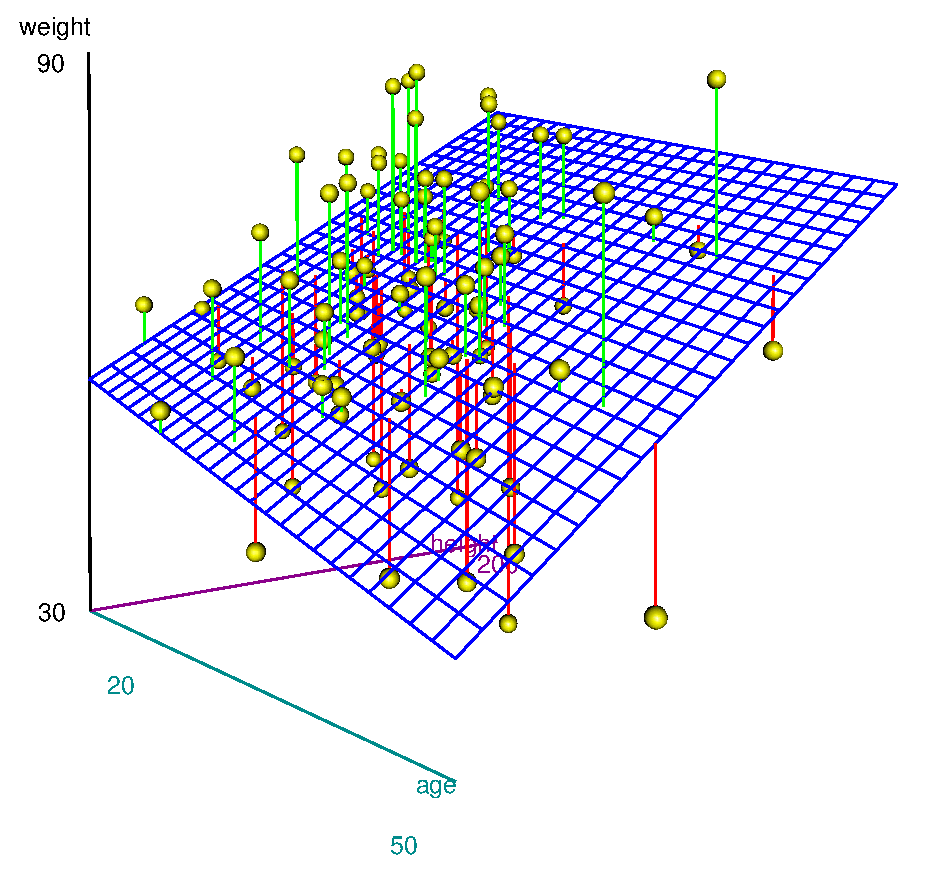
\includegraphics[width=8cm]{regrMult}
\vspace*{-1em}
\caption{Daten, Vorhersageebene und Residuen einer multiplen linearen Regression}
\label{fig:regrMult}
\end{figure}

%%%%%%%%%%%%%%%%%%%%%%%%%%%%%%%%%%%%%%%%%%%%%%%%%%%%%%%%%%%%%%%%%%
%%%%%%%%%%%%%%%%%%%%%%%%%%%%%%%%%%%%%%%%%%%%%%%%%%%%%%%%%%%%%%%%%%
\subsection{Modell verändern}
\label{sec:regrUpdate}
%%%%%%%%%%%%%%%%%%%%%%%%%%%%%%%%%%%%%%%%%%%%%%%%%%%%%%%%%%%%%%%%%%
%%%%%%%%%%%%%%%%%%%%%%%%%%%%%%%%%%%%%%%%%%%%%%%%%%%%%%%%%%%%%%%%%%

\index{Regression!Modell verändern}
\index[func]{update()@\lstinline{update()}}
Möchte man ein bereits berechnetes Modell nachträglich verändern, ihm etwa einen weiteren Prädiktor hinzufügen, kann dies mit \lstinline!update()! geschehen. Bei sehr umfassenden Modellen kann dies numerisch effizienter sein, als ein Modell vollständig neu berechnen zu lassen.
\begin{lstlisting}
update(<<lm-Modell>>, . ~ . + <<weiterer Prädiktor>>)
\end{lstlisting}

Als erstes Argument wird das zu erweiternde Modell eingetragen. In der folgenden Modellformel steht der \lstinline!.! vor der \lstinline!~! für die bisher verwendeten Kriterien, jener nach der \lstinline!~! für alle bisher verwendeten Prädiktoren. Die Formel \lstinline!. ~ .! signalisiert also, dass alle bisherigen Krtierien und Prädiktoren beizubehalten sind. Jeder weitere Prädiktor wird dann mit einem \lstinline!+! angefügt. Das Ergebnis von \lstinline!update()! ist das aktualisierte Modell.
\begin{lstlisting}
# füge sport als zusätzlichen Prädiktor hinzu
> (fitHAS <- update(fitHA, . ~ . + sport))     # gekürzte Ausgabe ...
Coefficients:
(Intercept)  height      age    sport
     8.1012  0.5149  -0.2866  -0.4160
\end{lstlisting}

Auf die gleiche Weise wie Prädiktoren hinzugefügt werden können, lassen sie sich auch entfernen, wobei statt des \lstinline!+! ein \lstinline!-! zu verwenden ist.
\begin{lstlisting}
# entferne Prädiktor height
> (fitAS <- update(fitHAS, . ~ . - height))     # gekürzte Ausgabe ...
Coefficients:
(Intercept)      age    sport
    98.5145  -0.2459  -0.4452

> (fitH <- update(fitHA,  . ~ . - age))         # entferne age ...
\end{lstlisting}

%%%%%%%%%%%%%%%%%%%%%%%%%%%%%%%%%%%%%%%%%%%%%%%%%%%%%%%%%%%%%%%%%%
%%%%%%%%%%%%%%%%%%%%%%%%%%%%%%%%%%%%%%%%%%%%%%%%%%%%%%%%%%%%%%%%%%
\subsection{Modelle vergleichen und auswählen}
\label{sec:regrCmp}
%%%%%%%%%%%%%%%%%%%%%%%%%%%%%%%%%%%%%%%%%%%%%%%%%%%%%%%%%%%%%%%%%%
%%%%%%%%%%%%%%%%%%%%%%%%%%%%%%%%%%%%%%%%%%%%%%%%%%%%%%%%%%%%%%%%%%

\index{Regression!Modellvergleich}
\index{Regression!hierarchische}
Existieren bei einer multiplen Regression viele potentielle Prädiktoren, stellt sich die Frage, welche letztlich im Modell berücksichtigt werden sollen. In einem hierarchischen Vorgehen lässt sich dafür testen, inwieweit die Hinzunahme von Prädiktoren zu einer bedeutsamen Verbesserung der Modellpassung führt. Dies ist in Form von $F$-Tests über Modellvergleiche möglich, die die Veränderung der Residualvarianz in Abhängigkeit vom verwendeten Prädiktorensatz testen. Dabei lassen sich sinnvoll nur \emph{nested} Modelle mit demselben Kriterium vergleichen, bei denen der Prädiktorensatz eines eingeschränkten Modells vollständig im Prädiktorensatz des umfassenderen Modells enthalten ist, das zusätzlich noch weitere Prädiktoren berücksichtigt (Abschn.\ \ref{sec:multALMmodCmp}).

Um verschiedene Regressionsmodelle miteinander hinsichtlich der Quadratsumme der Residuen sowie Akaikes Informationskriterium AIC vergleichen zu können, lassen sich folgende Funktionen verwenden:
\index[func]{step()@\lstinline{step()}}
\index[func]{add1()@\lstinline{add1()}}
\index[func]{drop1()@\lstinline{drop1()}}
\begin{lstlisting}
 step(object=<<lm-Modell>>, scope=~ . + <<Prädiktoren>>, direction="both)
 add1(object=<<lm-Modell>>, scope=~ . + <<Prädiktoren>>, test="none")
drop1(object=<<lm-Modell>>, scope=~ . - <<Prädiktoren>>, test="none")
\end{lstlisting}

\lstinline!step()! berechnet im \emph{Stepwise}-Verfahren\index{Regression!Stepwise-Verfahren} die Auswirkung einer schrittweisen Modellveränderung durch Hinzunahme oder Weglassen eines Prädiktors auf den AIC-Wert als Vergleichskriterium für die Güte der Modellpassung. Als Ergebnis wird ein Modell zurückgegeben, das durch diese Schritte nicht substantiell verbessert werden kann.\footnote{Das Paket \lstinline!lmSubsets!\index[pack]{lmSubsets@\lstinline{lmSubsets}} \cite{Hofmann2020b} ermöglicht die automatisierte Auswahl aller Teilmengen von Prädiktoren. Beide Verfahren sind mit vielen inhaltlichen Problemen verbunden, für eine Diskussion und verschiedene Strategien zur Auswahl von Prädiktoren vgl.\ \citeA{Miller2002}. Für penalisierte Regressionsverfahren, die auch eine Auswahl von Prädiktoren vornehmen, s.\ Abschn.\ \ref{sec:lmRob}.}

Dazu prüft \lstinline!step()! sequentiell Teilmengen von denjenigen Prädiktoren der unter \lstinline!object! angegebenen Regression, die in \lstinline!scope! als Modellformel definiert werden. Diese Modellformel beginnt mit einer \lstinline!~! und enthält danach alle Prädiktoren aus \lstinline!object! (Voreinstellung \lstinline!~ .!) sowie ggf.\ weitere mit \lstinline!+! hinzuzufügende. Mit \lstinline!step="backward"! beginnt die Exploration der Modelle beim umfassendsten Modell und entfernt dann Prädiktoren (Rückwärts-Elimination), analog mit \lstinline!step="forward"! beim einfachsten Modell und fügt Prädiktoren hinzu (Vorwärts-Selektion). In der Voreinstellung \lstinline!direction="both"! können von Schritt zu Schritt Prädiktoren sowohl hinzugefügt als auch entfernt werden.
\begin{lstlisting}
# Vorwärts-Selektion
> step(fitH, scope="~ height + age + sport", direction="forward")
Start:  AIC=501.38
weight ~ height
        Df Sum of Sq     RSS    AIC
+ sport  1   12962.8  1495.1 276.48
+ age    1    1246.3 13211.6 494.37
<none>               14457.9 501.38

Step:  AIC=276.48
weight ~ height + sport
       Df Sum of Sq     RSS    AIC
+ age   1     515.5  979.64 236.20
<none>              1495.14 276.48

Step:  AIC=236.2
weight ~ height + sport + age
Coefficients:
(Intercept)       height        sport          age  
     8.1012       0.5149      -0.4160      -0.2866 
\end{lstlisting}

\lstinline!add1()! berechnet separat den Effekt der Hinzunahme jeweils eines unter \lstinline!scope! genannten Prädiktors zu einer unter \lstinline!object! angegebenen Regression. Die Änderung in der Quadratsumme der Residuen bei jedem Schritt kann inferenzstatistisch geprüft werden, indem das Argument \lstinline!test="F"! gesetzt wird. Das einfachste Modell, in dem kein Prädiktor berücksichtigt wird, lautet \lstinline!<<Kriterium>> ~ 1! und sorgt dafür, dass für jeden Wert der konstante Mittelwert des Kriteriums vorhergesagt wird.
\begin{lstlisting}
# Vergleich: nur height als Prädiktor, sowie auch age bzw. sport
> add1(fitH, . ~ . + age + sport, test="F")
Single term additions
Model:
weight ~ height
        Df  Sum of Sq      RSS     AIC  F value     Pr(>F)
<none>                 14457.9  501.38
age      1     1246.3  13211.6  494.37     9.15   0.003183 **
sport    1    12962.8   1495.1  276.48   840.98  < 2.2e-16 ***
\end{lstlisting}

In der Zeile \lstinline!<none>! der Ausgabe finden sich die Kennwerte des eingeschränkten \lstinline!object! Modells, dessen Modellformel unter \lstinline!Model:! wiederholt wird. Die folgenden Zeilen nennen die Kennwerte der umfassenderen Modelle, bei denen zusätzlich jeweils einer der unter \lstinline!scope! genannten Prädiktoren berücksichtigt wird. Die Spalte \lstinline!Sum of Sq! führt die\index{Quadratsummen-Typen|see{Varianzanalyse}}\index{Varianzanalyse!Quadratsummen-Typen} sequentielle Quadratsumme vom Typ I des zusätzlichen Prädiktors beim Wechsel hin zu einem solchen Modell auf. Sie ist gleich der Differenz der in der Spalte \lstinline!RSS! genannten Quadratsummen der Residuen (\emph{residual sum of squares}) und damit ein Maß für die Reduktion an Fehlervarianz beim Modellwechsel. Die inferenzstatistischen Kennwerte finden sich in den Spalten \lstinline!Df! für die Differenz der Fehler-Freiheitsgrade vom eingeschränkten und umfassenderen Modell, \lstinline!F value! für den $F$-Wert und \lstinline!Pr(>F)! für den $p$-Wert.\footnote{Auf ähnliche Weise kann mit \lstinline!drop1()! die Quadratsumme vom Typ III eines Vorhersageterms als Effekt des Weglassens jeweils eines Prädiktors berechnet werden (Abschn.\ \ref{sec:ssTypes}).}

Der $F$-Wert ergibt sich als Quotient der angegebenen Quadratsumme geteilt durch die Differenz der Fehler-Freiheitsgrade und der Residual-Quadratsumme des umfassenderen Modells geteilt durch ihre Freiheitsgrade (Abschn.\ \ref{sec:multALMtest}). Die Fehler-Freiheitsgrade eines Modells berechnen sich als Differenz zwischen der Stichprobengröße und der Anzahl zu schätzender Parameter. Hier sind dies im eingeschränkten Modell mit einem Regressionsgewicht und dem absoluten Term zwei, in jedem Modell mit einem zusätzlichen Prädiktor entsprechend drei.
\begin{lstlisting}
# RSS Zeile <none>: Prädiktor height
> (rssH <- sum(residuals(lm(weight ~ height))^2))
[1] 14457.9

# RSS Zeile age: Prädiktoren height und age
> (rssHA <- sum(residuals(lm(weight ~ height + age))^2))
[1] 13211.64

# RSS Zeile sport: Prädiktoren height und sport
> (rssHS <- sum(residuals(lm(weight ~ height + sport))^2))
[1] 1495.140

# Fehler-Freiheitsgrade der drei Modelle
> dfEH  <- N - (1+1)                # eingeschränktes Modell
> dfEHA <- dfEHS <- N - (2+1)       # beide umfassenderen Modelle

# mittlere partielle Effekt-QS für Hinzunahme von age
> MSha <- (rssH - rssHA) / (dfEH - dfEHA)

# mittlere Residual-QS umfassenderes Modell: Prädiktoren height und age
> MSEha <- rssHA / dfEHA

# F-Wert für Effekt der Hinzunahme von age
> (Fha <- MSha / MSEha)
[1] 9.150025

# analog für Hinzunahme von sport
> MShs  <- (rssH - rssHS) / (dfEH - dfEHS)
> MSEhs <- rssHS / dfEHS
> (Fhs  <- MShs / MSEhs)
[1] 840.9835
\end{lstlisting}

Die Spalte \lstinline!AIC! listet den Wert von Akaikes Informationskriterium für beide Modelle auf.

Um nested Modelle gegeneinander zu testen, die sich um mehr als einen Prädiktor unterscheiden, können mit \lstinline!lm()! erstellte Regressionen an die\index[func]{anova()@\lstinline{anova()}} \lstinline!anova()! Funktion übergeben werden, die sich auch für Varianzanalysen eignet (Abschn.\ \ref{sec:anova}). Die Modelle müssen sich auf dieselben Beobachtungen beziehen -- bei fehlenden Werten ist sicherzustellen, dass in beide Modelle dieselben Beobachtungen einfließen.
\begin{lstlisting}
anova(<<eingeschränktes lm-Modell>>, <<umfassenderes lm-Modell>>)
\end{lstlisting}

Im Beispiel soll das Kriterium \lstinline!weight! entweder nur durch \lstinline!height!, oder aber durch alle drei Prädiktoren vorhergesagt werden.
\begin{lstlisting}
> anova(fitH, fitHAS)       # F-Test für Hinzunahme von age und sport
Analysis of Variance Table
Model 1: weight ~ height
Model 2: weight ~ height + age + sport
  Res.Df      RSS  Df  Sum of Sq      F     Pr(>F)
1     98  14457.9
2     96    979.6   2      13478  660.4  < 2.2e-16 ***
\end{lstlisting}

In der Ausgabe wird in der Spalte \lstinline!RSS! die Residual-Quadratsumme für jedes Modell aufgeführt, die zugehörigen Freiheitsgrade in der Spalte \lstinline!Res.Df!. In der Spalte \lstinline!Df! steht deren Differenz, um wie viele zu schätzende Parameter sich die Modelle also unterscheiden. Die Reduktion der Residual-Quadratsumme beim Wechsel zum umfassenderen Modell findet sich in der Spalte \lstinline!Sum of Sq!, daneben der zugehörige $F$-Wert (\lstinline!F!) und $p$-Wert (\lstinline!Pr(>F)!).

%%%%%%%%%%%%%%%%%%%%%%%%%%%%%%%%%%%%%%%%%%%%%%%%%%%%%%%%%%%%%%%%%%
%%%%%%%%%%%%%%%%%%%%%%%%%%%%%%%%%%%%%%%%%%%%%%%%%%%%%%%%%%%%%%%%%%
\subsection{Moderierte Regression}
\label{sec:regrMod}
%%%%%%%%%%%%%%%%%%%%%%%%%%%%%%%%%%%%%%%%%%%%%%%%%%%%%%%%%%%%%%%%%%
%%%%%%%%%%%%%%%%%%%%%%%%%%%%%%%%%%%%%%%%%%%%%%%%%%%%%%%%%%%%%%%%%%

\index{Regression!Moderation}
\index{Regression!Interaktion}
Bei der multiplen Regression kann die Hypothese bestehen, dass die theoretischen Regressionsparameter eines Prädiktors von der Ausprägung eines anderen Prädiktors abhängen \cite{Aiken1991}. Im Rahmen eines einfachen kausalen Einflussmodells mit einem Prädiktor $X_{1}$, einem Kriterium $Y$ und einer Drittvariable $X_{2}$ ließe sich etwa vermuten, dass der Einfluss von $X_{1}$ auf $Y$ davon abhängt, wie $X_{2}$ ausgeprägt ist.\footnote{Für Hinweise zur Analyse komplexerer Kausalmodelle s.\ Abschn.\ \ref{sec:multFA}, Fußnote \ref{ftn:structEqMod}.} Bei quantitativen Variablen spricht man dann von einer \emph{Moderation}, während man im Rahmen einer Varianzanalyse mit mehreren Faktoren den Begriff der \emph{Interaktion} verwendet (Abschn.\ \ref{sec:CRFpq}). Die Vorhersagegleichung der Regression mit zwei Prädiktoren erweitert sich durch den Interaktionsterm zu $\hat{Y} = b_{0} + b_{1} X_{1} + b_{2} X_{2} + b_{3} (X_{1} X_{2})$. Es wird also ein weiterer Vorhersageterm hinzugefügt, der gleich dem Produkt beider Prädiktoren ist. Im Aufruf von \lstinline!lm()! geschieht dies durch Aufnahme des Terms \lstinline!X1:X2! in die Modellformel.

Moderator sei hier das Alter bei der Regression des Körpergewichts auf die Körpergröße.
\begin{lstlisting}
# Modell mit zentrierten Prädiktoren und Interaktionsterm
> heightC <- c(scale(height, center=TRUE, scale=FALSE))
> ageC    <- c(scale(age,    center=TRUE, scale=FALSE))
> fitHAi  <- lm(weight ~ heightC + ageC + heightC:ageC)
> coef(summary(fitHAi))
              Estimate  Std. Error  t value  Pr(>|t|)
(Intercept)   63.95331     1.17188   54.573   < 2e-16 ***
heightC        0.85591     0.16413    5.215  1.06e-06 ***
ageC          -0.44947     0.14696   -3.058   0.00288 **
heightC:ageC   0.01509     0.01945    0.776   0.43986
\end{lstlisting}

Im umgeformten Modell $\hat{Y} = (b_{0} + b_{2} X_{2}) + (b_{1} + b_{3} X_{2}) X_{1}$ wird ersichtlich, dass es sich wie jenes der einfachen linearen Regression des Prädiktors $X_{1}$ schreiben lässt, wobei $y$-Achsenabschnitt und Steigungsparameter nun lineare Funktionen des als Moderator betrachteten Prädiktors $X_{2}$ sind. Der Term $b_{0s} = b_{0} + b_{2} X_{2}$ wird als \emph{simple intercept}, $b_{1s} = b_{1} + b_{3} X_{2}$ als \emph{simple slope} oder auch als \emph{marginal effect} bezeichnet. Für einen festen Wert des Moderators $X_{2}$ ergeben sich für $b_{0s}$ und $b_{1s}$ konkrete Werte. Um einen Eindruck von der Bandbreite der Parameterschätzungen zu gewinnen, bieten sich für die Wahl fester Werte von $X_{2}$ dessen Mittelwert sowie die Werte $\pm$ eine Standardabweichung um den Mittelwert an. Eine andere Möglichkeit sind der Median sowie das erste und dritte Quartil von $X_{2}$.

\index[func]{emtrends()@\lstinline{emtrends()}}
Die Funktion \lstinline!emtrends()! aus dem Paket \lstinline!emmeans!\index[pack]{emmeans@\lstinline{emmeans}|textbf} \cite{Lenth2019} berechnet die simple slopes für vorgegebene Werte des Moderators -- auch für Modelle mit noch weiteren Prädiktoren, die nicht Teil einer Interaktion sind.
\begin{lstlisting}
emtrends(<<lm-Modell>>, ~ <<Moderator>>, var="<<Prädiktor>>",
         at=list(<<Moderator>>=<<Werte>>))
\end{lstlisting}

Als erstes Argument ist ein mit \lstinline!lm()! erstelltes Regressionsmodell zu übergeben. Das zweite Argument erwartet eine Modellformel, in der $X_{2}$ als Moderator auf der rechten Seite der \lstinline!~! steht und die linke Seite leer ist. Für \lstinline!var! ist der Name des moderierten Prädiktors $X_{1}$ zu nennen. Für welche Werte des Moderators $X_{2}$ die simple slopes $b_{1s}$ berechnet werden sollen, kontrolliert \lstinline!at!: Dies ist eine Liste mit dem Vektor der gewünschten Werte als Komponente, die den Namen des Moderators trägt.

\index[func]{test()@\lstinline{test()}}
Das Ergebnis ist in der Spalte \lstinline!<<Prädiktor>>.trend! eine Übersicht über die geschätzten simple slopes $b_{1s}$ mit jeweils zugehörigem Standardfehler und Konfidenzintervall. Für den zweiseitigen $t$-Test ist das zurückgegebene Objekt zu speichern und an \lstinline!test()! zu übergeben.
\begin{lstlisting}
> library(emmeans)                  # für emtrends(), test()
> ageC_vals <- c(-sd(ageC), 0, sd(ageC))
> (et <- emtrends(fitHAi, ~ageC, var="heightC",
+                 at=list(ageC=ageC_vals)))
 ageC heightC.trend    SE df lower.CL upper.CL
-8.03         0.735 0.230 96    0.278     1.19
 0.00         0.856 0.164 96    0.530     1.18
 8.03         0.977 0.223 96    0.535     1.42

 > test(et)
 ageC heightC.trend    SE df t.ratio p.value
-8.03         0.735 0.230 96   3.190  0.0019
 0.00         0.856 0.164 96   5.215  <.0001
 8.03         0.977 0.223 96   4.388  <.0001
\end{lstlisting}

Das von \lstinline!emtrends()! zurückgegebene Objekt wird von \lstinline!plot()! akzeptiert, um die simple slopes $b_{1s}$ und ihre jeweiligen Konfidenzintervalle in Abhängigkeit von der Ausprägung des Moderators in einem Diagramm darzustellen (Abb.\ \ref{fig:regrModeration}). Das Ergebnis ist ein mit dem Paket \lstinline!ggplot2! erstelltes Diagramm, das sich mit den in Kap.\ \ref{sec:ggplot} vorgestellten Methoden anpassen lässt.
\begin{lstlisting}
# Werte des Moderators, für die simple slopes des Prädiktors
# gezeigt werden sollen
> ageC_vals <- seq(-15, 20, by=5)
> et_plot   <- emtrends(fitHAi, ~ageC, var="heightC",
+                       at=list(ageC=ageC_vals))

> plot(et_plot) + coord_flip() + theme_bw()
\end{lstlisting}

Zur Darstellung der vorhergesagten Werte des Regressionsmodells dient die Funktion \lstinline!emmip()!. Sie erlaubt es auf einfache Weise, verschiedene Vorhersagegeraden für den Zusammenhang von Zielgröße und Prädiktor getrennt für einzelne Werte des Moderators darzustellen.
\index[func]{emmip()@\lstinline{emmip()}}
\begin{lstlisting}
emmip(<<lm-Modell>>, <<Moderator>> ~ <<Prädiktor>>,
      at=list(<<Moderator>>=<<Werte>>, <<Prädiktor>>=<<Werte>>),
      CIs=TRUE, plotit=TRUE)
\end{lstlisting}

Als erstes Argument ist ein mit \lstinline!lm()! erstelltes Regressionsmodell zu übergeben. Das zweite Argument erwartet eine Modellformel mit dem Moderator $X_{2}$ auf der linken Seite der \lstinline!~! steht und dem Prädiktor $X_{1}$ auf der rechten Seite. Sollen Konfidenzintervalle für die Vorhersage gezeigt werden, ist \lstinline!CIs=TRUE! zu setzen. Für welche Werte des Moderators sowie des Prädiktors die Vorhersagegeraden gezeigt werden sollen, kontrolliert \lstinline!at!: Dies ist eine Liste mit jeweils einem Vektor der gewünschten Werte als Komponente für den Moderator und für den Prädiktor. Die Werte des Prädiktors werden auf der $x$-Achse abgetragen, die Werte des Moderators werden zur Definition separater Linien verwendet. Mit \lstinline!plotit=FALSE! erzeugt der Aufruf kein Diagramm, sondern liefert nur die berechneten Daten zurück, die dann für ein selbst erstelltes Diagramm verwendet werden können (Abb.\ \ref{fig:regrModeration}).
\begin{lstlisting}
> r_hC <- range(heightC)
> d_ip <- emmip(fitHAi, ageC ~ heightC,
+               at=list(heightC=seq(r_hC[1], r_hC[2], length=20),
+                       ageC=c(-sd(ageC), 0, sd(ageC))),
+               CIs=TRUE, plotit=FALSE) |>
+      transform(ageC=sprintf("%.2f", ageC))

> library(ggplot2)                         # für ggplot()
> ggplot(d_ip, aes(x=heightC, y=yvar, group=ageC,
+                  color=ageC, fill=ageC,
+                  ymin=LCL, ymax=UCL)) +
+     geom_ribbon(alpha=0.4, linetype="blank") +
+     geom_line() +
+     ylab("Prediction") +
+     theme_bw()
\end{lstlisting}

\begin{figure}[ht]
\centering
\includegraphics[width=12.5cm]{regrModeration}
\vspace*{-0.5em}
\caption{Simple slopes und Vorhersagegeraden in der Regression mit Moderator}
\label{fig:regrModeration}
\end{figure}

Es folgt die manuelle Kontrolle.
\begin{lstlisting}
> coeffs <- coef(fitHAi)              # extrahiere Koeffizienten
> b0 <- coeffs[1]                     # y-Achsenabschnitt
> b1 <- coeffs[2]
> b2 <- coeffs[3]
> b3 <- coeffs[4]

# bedingte y-Achsenabschnitte
> b0 + b2*(mean(ageC) - sd(ageC))     # für M - 1sd ...
> b0 + b2* mean(ageC)                 # für M ...
> b0 + b2*(mean(ageC) + sd(ageC))     # für M + 1sd ...

# bedingte Steigungen
> b1 + b3*(mean(ageC) - sd(ageC))     # für M - 1sd ...
> b1 + b3* mean(ageC)                 # für M ...
> b1 + b3*(mean(ageC) + sd(ageC))     # für M + 1sd ...
\end{lstlisting}

%%%%%%%%%%%%%%%%%%%%%%%%%%%%%%%%%%%%%%%%%%%%%%%%%%%%%%%%%%%%%%%%%%
%%%%%%%%%%%%%%%%%%%%%%%%%%%%%%%%%%%%%%%%%%%%%%%%%%%%%%%%%%%%%%%%%%
\section{Regressionsmodelle auf andere Daten anwenden}
\label{sec:predict}
%%%%%%%%%%%%%%%%%%%%%%%%%%%%%%%%%%%%%%%%%%%%%%%%%%%%%%%%%%%%%%%%%%
%%%%%%%%%%%%%%%%%%%%%%%%%%%%%%%%%%%%%%%%%%%%%%%%%%%%%%%%%%%%%%%%%%

\index{Regression!Konfidenzintervall}
\index{Regression!Toleranzintervall}
\index[func]{predict()@\lstinline{predict()}}
\lstinline!predict()! wendet ein von \lstinline!lm()! angepasstes Regressionsmodell auf neue Daten an, um für sie die Vorhersage $\hat{Y}$ zu berechnen (vgl.\ \lstinline!?predict.lm!).
\begin{lstlisting}
predict(object=<<lm-Modell>>, newdata=<<Datensatz>>, se.fit=FALSE,
        interval=NULL, level=<<Breite Konfidenzintervall>>)
\end{lstlisting}

Als erstes Argument ist ein von \lstinline!lm()! erzeugtes Objekt zu übergeben. Werden alle weiteren Argumente weggelassen, liefert die Funktion die Vorhersage für die ursprünglichen Prädiktorwerte zurück, also \lstinline!fitted(<<lm-Modell>>)!. Wird unter \lstinline!newdata! ein Datensatz übergeben, der Variablen mit denselben Namen wie jene der ursprünglichen Prädiktoren enthält, so wird $\hat{Y}$ für die Werte dieser neuen Variablen berechnet.\footnote{Handelt es sich etwa im Rahmen einer Kovarianzanalyse (Abschn.\ \ref{sec:ancova}) um einen kategorialen Prädiktor -- ein Objekt der Klasse \lstinline!factor!, so muss die zugehörige Variable in \lstinline!newdata! dieselben Stufen in derselben Reihenfolge beinhalten wie die Variable des ursprünglichen Modells -- selbst wenn nicht alle Faktorstufen tatsächlich als Ausprägung vorkommen.} Wenn die Modellformel Transformationen von Variablen -- etwa mit \lstinline!I()! (Abschn.\ \ref{sec:formula}) oder \lstinline!poly()! (Abschn.\ \ref{sec:lmNonlin}) -- enthält, werden diese von \lstinline!predict()! automatisch aus den Variablen des Datensatzes gebildet. Sollen die Standardabweichungen für $\hat{Y}$ ermittelt werden, ist \lstinline!se.fit=TRUE! zu setzen.

Mit dem Argument \lstinline!interval="confidence"! berechnet \lstinline!predict()! zusätzlich für jeden Wert der Prädiktorvariablen die Grenzen des punktweisen Konfidenzintervalls für den geschätzten \emph{Parameter}, hier also den bedingten Erwartungswert von $Y$. Die Breite des Konfidenzintervalls wird mit \lstinline!level! kontrolliert. Mit \lstinline!interval="prediction"! erhält man stattdessen die Grenzen des Toleranzintervalls für die Vorhersage einer neuen \emph{Beobachtung} von $Y$. Das Toleranzintervall spiegelt einerseits die Unsicherheit der Parameterschätzer, andererseits auch die geschätzte Streuung $\hat{\sigma}$ von $Y$ um den bedingten Erwartungswert (Standardschätzfehler) wider. Die Ausgabe erfolgt in Form einer Matrix, deren erste Spalte (\lstinline!fit!) die Vorhersage ist, während die beiden weiteren Spalten untere (\lstinline!lwr!) und obere Grenzen (\lstinline!upr!) des Vertrauensbereichs nennen.

Im Beispiel des Modells mit nur dem Prädiktor \lstinline!height! wird für den Aufruf von \lstinline!predict()! zunächst ein Datensatz mit einer passend benannten Variable erzeugt.
\begin{lstlisting}
> newHeight <- c(177, 150, 192, 189, 181)         # neue Daten
> newDf     <- data.frame(height=newHeight)       # Datensatz
> predict(fitH, newDf, interval="prediction", level=0.95)
       fit       lwr        upr
1 66.00053  41.76303   90.23803
2 43.68101  18.07599   69.28604
3 78.40026  53.47502  103.32550
4 75.92032  51.21385  100.62678
5 69.30713  44.98704   93.62721

# Kontrolle der Vorhersage durch Extrahieren der Regressionsparameter
# und Einsetzen der neuen Daten in die Vorhersagegleichung
> (coeffs <- coef(fitH))                          # Parameter
(Intercept)     height
-80.3163014  0.8266488

> coeffs[2]*newHeight + coeffs[1]                 # Vorhersage
[1] 66.00053 43.68101 78.40026 75.92032 69.30713
\end{lstlisting}

Der Vertrauensbereich um die Vorhersage für die ursprünglichen Daten lässt sich auch grafisch darstellen (Abb.\ \ref{fig:regrCI}).
\begin{lstlisting}
> plot(weight ~ height, pch=20, xlab="Prädiktor",
+      ylab="Kriterium und Vorhersage", xaxs="i",
+      main="Daten und Vorhersage durch Regression")

# Vertrauensintervall um Vorhersage für Originaldaten
> predOrg <- predict(fitH, interval="confidence", level=0.95)
> hOrd    <- order(height)
> polygon(c(height[hOrd],         height[rev(hOrd)]),
+         c(predOrg[hOrd, "lwr"], predOrg[rev(hOrd), "upr"]),
+         border=NA, col=rgb(0.7, 0.7, 0.7, 0.6))

> abline(fitH, col="blue")                        # Regressionsgerade
> legend(x="bottomright", legend=c("Daten", "Vorhersage",
+        "Vertrauensbereich"), pch=c(20, NA, NA), lty=c(NA, 1, 1),
+        lwd=c(NA, 1, 8), col=c("black", "blue", "gray"))
\end{lstlisting}

\begin{figure}[ht]
\centering
\includegraphics[width=8cm]{regrCI}
\vspace*{-1em}
\caption{Lineare Regression: Prädiktor, Kriterium und Vorhersage mit Vertrauensbereich}
\label{fig:regrCI}
\end{figure}

%%%%%%%%%%%%%%%%%%%%%%%%%%%%%%%%%%%%%%%%%%%%%%%%%%%%%%%%%%%%%%%%%%
%%%%%%%%%%%%%%%%%%%%%%%%%%%%%%%%%%%%%%%%%%%%%%%%%%%%%%%%%%%%%%%%%%
\section{Regressionsdiagnostik}
\label{sec:regrDiag}
%%%%%%%%%%%%%%%%%%%%%%%%%%%%%%%%%%%%%%%%%%%%%%%%%%%%%%%%%%%%%%%%%%
%%%%%%%%%%%%%%%%%%%%%%%%%%%%%%%%%%%%%%%%%%%%%%%%%%%%%%%%%%%%%%%%%%

\index{Regression!Regressionsdiagnostik}
\index{Regression!Voraussetzungen}
Einer konventionellen Regressionsanalyse liegen verschiedene Annahmen zugrunde, deren Gültigkeit vorauszusetzen ist, damit die berechneten Standardfehler der Parameterschätzungen und die $p$-Werte korrekt sind (Abschn.\ \ref{sec:multALMpred}). Dazu gehören bedingte Normalverteiltheit und gemeinsame Unabhängigkeit der Messfehler des Kriteriums, die zudem unabhängig von den Prädiktoren sein müssen. Hinzu kommt die \emph{Homoskedastizität}, also die Gleichheit aller bedingten Fehlervarianzen (Abb.\ \ref{fig:regrHomSc}).

Mit Hilfe der Regressionsdiagnostik soll zum einen geprüft werden, ob die Daten mit den gemachten Annahmen konsistent sind. Zum anderen kann die Parameterschätzung der konventionellen Regression durch wenige Ausreißer überproportional beeinflusst werden. Daher ist es von Interesse, diese zu identifizieren und den Einfluss einzelner Beobachtungen auf das Ergebnis zu bestimmen. Schließlich ist in der multiplen Regression das Ausmaß der \emph{Multikollinearität} bedeutsam, also die lineare Abhängigkeit der Prädiktoren untereinander. Für eine ausführliche Darstellung vgl.\ \citeA{Fox2002} sowie das zugehörige Paket \lstinline!car!\index[pack]{car@\lstinline{car}} für Funktionen, mit denen sich eine Vielzahl diagnostischer Diagramme erstellen lassen.

%%%%%%%%%%%%%%%%%%%%%%%%%%%%%%%%%%%%%%%%%%%%%%%%%%%%%%%%%%%%%%%%%%
%%%%%%%%%%%%%%%%%%%%%%%%%%%%%%%%%%%%%%%%%%%%%%%%%%%%%%%%%%%%%%%%%%
\subsection{Extremwerte, Ausreißer und Einfluss}
\label{sec:regrInfluence}
%%%%%%%%%%%%%%%%%%%%%%%%%%%%%%%%%%%%%%%%%%%%%%%%%%%%%%%%%%%%%%%%%%
%%%%%%%%%%%%%%%%%%%%%%%%%%%%%%%%%%%%%%%%%%%%%%%%%%%%%%%%%%%%%%%%%%

\index{Daten!Ausreißer}
\index{Daten!Extremwerte}
Unter einem Ausreißer sind hier Beobachtungen zu verstehen, deren Kriteriumswert stark vom Kriteriumswert anderer Beobachtungen abweicht, die ähnliche Prädiktorwerte besitzen. Extremwerte einer gegebenen Variable zeichnen sich dadurch aus, dass sie weit außerhalb der Verteilung der übrigen Beobachtungen liegen. Die grafische Beurteilung, ob Extremwerte vorliegen, lässt sich getrennt für jede Variable etwa durch Histogramme oder Boxplots der $z$-standardisierten Variable durchführen (Abb.\ \ref{fig:regrInfl}; Abschn.\ \ref{sec:hist}, \ref{sec:boxplot}, \ref{sec:ggplotBoxplot}).

Als numerische Indikatoren eignen sich die $z$-standardisierten Werte, an denen abzulesen ist, wie viele Streuungseinheiten ein Wert vom Mittelwert entfernt ist. Als numerisches Maß der multivariaten Extremwertanalyse bietet sich die Mahalanobisdistanz als Verallgemeinerung der $z$-Transformation an (Abschn.\ \ref{sec:mahaDist}). Sie repräsentiert den Abstand eines Datenpunkts zum Zentroid der Verteilung, wobei der Gesamtform der Verteilung i.\,S.\ der Kovarianzmatrix Rechnung getragen wird. Für die grafische Darstellung der gemeinsamen Verteilung von zwei oder drei Variablen s.\ Abschn.\ \ref{sec:distr2var}, \ref{sec:3dPlot}.\footnote{\index{robuste Verfahren!Ausreißer identifizieren}Da Extremwerte die Lage und Streuung der Daten mit beeinflussen, sollten hierfür evtl.\ robuste Schätzer in Betracht gezogen werden (Abschn.\ \ref{sec:varRob}). Robuste Schätzungen für die Kovarianzmatrix können etwa an das Argument \lstinline!cov! von \lstinline!mahalanobis()! übergeben werden. Für fortgeschrittene Tests, ob Ausreißer in multivariaten Daten vorliegen, vgl.\ \lstinline!aq.plot()!\index[func]{aq.plot()@\lstinline{aq.plot()}} und\index[func]{pcout()@\lstinline{pcout()}} \lstinline!pcout()! aus dem Paket \lstinline!mvoutlier!\index[pack]{mvoutlier@\lstinline{mvoutlier}} \cite{Filzmoser2011b}.}
\begin{lstlisting}
> Xpred <- cbind(height, age, sport)      # Prädiktoren als Datenmatrix
> Xz    <- scale(Xpred)                   # z-Transformierte
> boxplot(Xz, main="Verteilung standardisierte Prädiktoren")
> summary(Xz)
        height              age                 sport
Min.   :-2.534e+00  Min.   :-1.952e+00  Min.   :-1.796e+00
1st Qu.:-6.040e-01  1st Qu.:-7.110e-01  1st Qu.:-6.884e-01
Median : 1.075e-02  Median :-1.069e-01  Median :-9.467e-02
Mean   : 1.781e-15  Mean   :-8.978e-17  Mean   : 1.087e-16
3rd Qu.: 6.338e-01  3rd Qu.: 7.411e-01  3rd Qu.: 6.519e-01
Max.   : 2.200e+00  Max.   : 2.839e+00  Max.   : 2.727e+00

# Mahalanobis-Distanz der Beobachtungen zum Zentroid der Prädiktoren
> ctrX   <- colMeans(Xpred)               # Zentroid
> sX     <- cov(Xpred)                    # Kovarianzmatrix
> mahaSq <- mahalanobis(Xpred, ctrX, sX)  # quadrierte M-Distanzen
> summary(sqrt(mahaSq))
  Min.  1st Qu.  Median    Mean  3rd Qu.    Max.
0.2855   1.1640  1.5940  1.5970   1.9750  3.3090
\end{lstlisting}

\index{Regression!Hebelwert}
Durch Extremwerte oder Ausreißer wird die ermittelte Vorhersagegleichung womöglich in dem Sinne verzerrt, dass sie die Mehrzahl der Daten nicht mehr gut repräsentiert. Um den Einfluss der einzelnen Beobachtungen auf die Parameterschätzungen der Regression direkt zu quantifizieren, existieren verschiedene Kennwerte, darunter der Hebelwert $h$ (\emph{leverage}). $h$ wird durch\index[func]{hatvalues()@\lstinline{hatvalues()}} \lstinline!hatvalues(<<lm-Modell>>)! berechnet.\footnote{Zudem ist $h_{i}$ gleich dem $i$-ten Eintrag $\bm{H}_{ii}$ in der Diagonale der\index{Regression!Hat-Matrix} Hat-Matrix $\bm{H}$ (Abschn.\ \ref{sec:regrMultAn}).} Für Modelle, die einen absoluten Term $b_{0}$ einschließen, kann $h$ Werte im Intervall $[\frac{1}{n}, 1]$ annehmen, wobei $n$ die Anzahl an Beobachtungen ist. Der Mittelwert ist dann gleich $\frac{p+1}{n}$ mit $p+1$ als Anzahl zu schätzender Parameter der Regression ($p$ Prädiktoren sowie absoluter Term). Um besonders große Hebelwerte zu identifizieren, kann ihre Verteilung etwa über ein Histogramm oder einen \emph{spike-plot} veranschaulicht werden (Abb.\ \ref{fig:regrInfl}, Abschn.\ \ref{sec:plot}). Als numerisches Kriterium für auffällig große Hebelwerte dient bisweilen das Zwei- bis Dreifache seines Mittelwerts.
\begin{lstlisting}
> fitHAS <- lm(weight ~ height + age + sport)   # Regression
> h      <- hatvalues(fitHAS)                   # Hebelwerte
> hist(h, main="Histogramm der Hebelwerte")     # Histogramm
> summary(h)
   Min.  1st Qu.   Median     Mean  3rd Qu.     Max.
0.01082  0.02368  0.03568  0.04000  0.04942  0.12060
\end{lstlisting}

Zur Kontrolle lässt sich die Beziehung nutzen, dass die quadrierte Mahalanobisdistanz einer Beobachtung $i$ zum Zentroid der Prädiktoren gleich $(n-1) (h_{i} - \frac{1}{n})$ ist.
\begin{lstlisting}
> all.equal(mahaSq, (N-1) * (h - (1/N)), check.attributes=FALSE)
[1] TRUE
\end{lstlisting}

\index{Regression!Einfluss}
Die Indizes DfFITS bzw.\ DfBETAS liefern für jede Beobachtung ein standardisiertes Maß, wie stark sich die Vorhersagewerte (DfFITS) bzw.\ jeder geschätzte Parameter (DfBETAS) tatsächlich ändern, wenn die Beobachtung aus den Daten ausgeschlossen wird. In welchem Ausmaß sich dabei der Standardschätzfehler ändert, wird über das Verhältnis beider resultierenden Werte (mit bzw.\ ohne ausgeschlossene Beobachtung) ausgedrückt. Cooks Distanz ist ein weiteres Einflussmaß, das sich als $\frac{E^{2}}{\hat{\sigma}^{2} (1-h)^{2}} \cdot \frac{h}{p+1}$ berechnet, wobei $E$ für die Residuen $Y - \hat{Y}$ und $\hat{\sigma}$ für den Standardschätzfehler der Regression mit $p+1$ Parametern steht.

Mit\index[func]{influence.measures()@\lstinline{influence.measures()}} \lstinline!influence.measures(<<lm-Modell>>)! lassen sich die genannten Kennwerte gleichzeitig berechnen. Auffällige Beobachtungen können aus der zurückgegebenen Liste mit\index[func]{summary()@\lstinline{summary()}} \lstinline!summary()! extrahiert werden, wobei der Wert der abweichenden diagnostischen Größe durch einen Stern \lstinline!*! markiert ist.
\begin{lstlisting}
> inflRes <- influence.measures(fitHAS)    # Diagnosegrößen
> summary(inflRes)                         # auffällige Beobachtungen
Potentially influential observations of
lm(formula = weight ~ height + age + sport) :
    dfb.1  dfb.hght  dfb.age  dfb.sprt  dffit   cov.r    cook.d   hat
6   -0.05      0.07    -0.23      0.25   0.40    0.86_*    0.04  0.03
13  -0.21      0.21    -0.10      0.36   0.41    1.13_*    0.04  0.12_*
30   0.19     -0.23     0.17     -0.01  -0.42    0.74_*    0.04  0.02
31  -0.08      0.11    -0.08     -0.05   0.27    0.86_*    0.02  0.01
67   0.02     -0.02    -0.03      0.03  -0.05    1.17_*    0.00  0.11
72  -0.03      0.03     0.04      0.01   0.05    1.17_*    0.00  0.11
86   0.10     -0.16     0.60     -0.25   0.68_*  0.90      0.11  0.08
97  -0.01      0.01    -0.01      0.01   0.02    1.16_*    0.00  0.10
\end{lstlisting}

In der Ausgabe beziehen sich die Spalten \lstinline!dfb.<<Prädiktor>>! auf das DfBETA jedes Prädiktors (inkl.\ des absoluten Terms \lstinline!1! in der ersten Spalte), \lstinline!dffit! auf DfFITS, \lstinline!cov.r! auf das Verhältnis der Standardschätzfehler, \lstinline!cook.d! auf Cooks Distanz und \lstinline!hat! auf den Hebelwert. Für Funktionen zur separaten Berechnung der Maße vgl.\ \lstinline!?influence.measures!.
\begin{lstlisting}
> cooksDst <- cooks.distance(fitHAS)               # Cooks Distanz
> plot(cooksDst, main="Cooks Distanz", type="h")   # spike-plot

# manuelle Berechnung
> P   <- 3                                         # Anzahl Prädiktoren
> E   <- residuals(fitHAS)                         # Residuen
> MSE <- sum(E^2) / (N - (P+1))           # quadr. Standardschätzfehler
> CD  <- (E^2 / (MSE * (1-h)^2)) * (h / (P+1))     # Cooks Distanz
> all.equal(cooksDst, CD)                          # Kontrolle
[1] TRUE
\end{lstlisting}

Grafisch aufbereitete Informationen über den Einfluss einzelner Beobachtungen sowie über die Verteilung der Residuen (s.\,u.) liefert auch eine mit\index[func]{plot()@\lstinline{plot()}} \lstinline!plot(<<lm-Modell>>, which=1:6)! aufzurufende Serie von Diagrammen. Über das Argument \lstinline!which! können dabei einzelne Grafiken der Serie selektiv gezeigt werden. Vergleiche dazu auch\index[func]{influencePlot()@\lstinline{influencePlot()}} \lstinline!influencePlot()! und\index[func]{influenceIndexPlot()@\lstinline{influenceIndexPlot()}} \lstinline!influenceIndexPlot()! aus dem \index[pack]{car@\lstinline{car}} \lstinline!car! Paket.

\begin{figure}[ht]
\centering
\includegraphics[width=12.5cm]{regrInfl}
\vspace*{-0.5em}
\caption{Beurteilung von Extremwerten und Einflussgrößen in der Regression}
\label{fig:regrInfl}
\end{figure}

%%%%%%%%%%%%%%%%%%%%%%%%%%%%%%%%%%%%%%%%%%%%%%%%%%%%%%%%%%%%%%%%%%
%%%%%%%%%%%%%%%%%%%%%%%%%%%%%%%%%%%%%%%%%%%%%%%%%%%%%%%%%%%%%%%%%%
\subsection{Verteilungseigenschaften der Residuen}
\label{sec:regrResid}
%%%%%%%%%%%%%%%%%%%%%%%%%%%%%%%%%%%%%%%%%%%%%%%%%%%%%%%%%%%%%%%%%%
%%%%%%%%%%%%%%%%%%%%%%%%%%%%%%%%%%%%%%%%%%%%%%%%%%%%%%%%%%%%%%%%%%

Die Verteilung der Residuen in Abhängigkeit von einzelnen Prädiktoren kann in einer multiplen Regression das Verständnis der Zusammenhänge erleichtern. Das Paket \lstinline!car!\index[pack]{car@\lstinline{car}} bietet hierfür die Funktion \index[func]{residualPlots()@\lstinline{residualPlots()}}\lstinline!residualPlots()! mit zahlreichen Optionen (Abb.\ \ref{fig:regrResidPlot}).

\begin{lstlisting}
> library(car)                    # für residualPlots()
> residualPlots(fitHAS, tests=FALSE)
\end{lstlisting}

\begin{figure}[ht]
\centering
\includegraphics[width=12.5cm]{regrResidPlot}
\vspace*{-0.5em}
\caption{Prädiktor-Residuen Diagramme in der multiple Regression}
\label{fig:regrResidPlot}
\end{figure}

Anhand verschiedener grafischer Darstellungen der Residuen einer Regression lässt sich heuristisch beurteilen, ob die vorliegenden Daten mit den Voraussetzungen der Normalverteiltheit, Unabhängigkeit und Homoskedastizität der Messfehler vereinbar sind. Als Grundlage können die Residuen $E = Y - \hat{Y}$ selbst, oder aber zwei Transformationen von ihnen dienen: Die \emph{standardisierten} und \emph{studentisierten} Residuen besitzen eine theoretische Streuung von $1$ und ergeben sich als $\frac{E}{\hat{\sigma} \sqrt{1-h}}$, wobei $\hat{\sigma}$ eine Schätzung der theoretischen Fehlerstreuung ist (Abschn.\ \ref{sec:multALMpred}).

Für die standardisierten Residuen wird der Standardschätzfehler als globale Schätzung in der Rolle von $\hat{\sigma}$ verwendet, bei den studentisierten Residuen dagegen eine beobachtungsweise Schätzung $\hat{\sigma}_{i}$. Dabei wird im Fall \emph{extern} studentisierter Residuen (\emph{leave-one-out}) $\hat{\sigma}_{(i)}$ für jede Beobachtung $i$ auf Basis des Regressionsmodells berechnet, in das alle Daten bis auf die der $i$-ten Beobachtung einfließen. Für die im Folgenden aufgeführten Prüfmöglichkeiten werden oft standardisierte oder studentisierte Residuen $E$ gegenüber vorgezogen.

\lstinline!lm.influence()!\index[func]{lm.influence()@\lstinline{lm.influence()}} speichert $\hat{\sigma}_{(i)}$ in der Komponente \lstinline!sigma! der ausgegebenen Liste. Die Residuen selbst lassen sich mit \lstinline!residuals()! für $E$, \lstinline!rstandard()!\index[func]{rstandard()@\lstinline{rstandard()}} für die standardisierten und\index[func]{rstudent()@\lstinline{rstudent()}} \lstinline!rstudent()! für die extern studentisierten Residuen ermitteln (s.\ auch Abschn.\ \ref{sec:LOOCV}). Bei allen Funktionen ist als Argument ein von \lstinline!lm()! erstelltes Modell zu übergeben.
\begin{lstlisting}
> Estnd <- rstandard(fitHAS)                # standardisierte Residuen
> all.equal(Estnd, E / sqrt(MSE * (1-h)))   # manuelle Kontrolle
[1] TRUE

# studentisierte Residuen und manuelle Kontrolle
> Estud <- rstudent(fitHAS)
> all.equal(Estud, E / (lm.influence(fitHAS)$sigma * sqrt(1-h)))
[1] TRUE
\end{lstlisting}

Für eine visuell-exploratorische Beurteilung der Normalverteiltheit wird die Verteilung der bevorzugten Residuen-Variante mit einem Histogramm der relativen Klassenhäufigkeiten dargestellt, dem die Dichtefunktion der Standardnormalverteilung hinzugefügt wurde (Abb.\ \ref{fig:regrResid}, Abschn.\ \ref{sec:gghist}, \ref{sec:ggplotAddElem}). Das Histogramm sollte in seiner Form nicht stark von der Dichtefunktion abweichen. Zudem lässt sich ein Q-Q-plot nutzen, um die empirischen Quantile der Residuen mit jenen der Standardnormalverteilung zu vergleichen. Die Datenpunkte sollten hier auf einer Geraden liegen (Abb.\ \ref{fig:regrResid}, Abschn.\ \ref{sec:qq}). Für einen inferenzstatistischen Test mit der $\text{H}_{0}$, dass Normalverteilung vorliegt, bietet sich jener nach Shapiro-Wilk an (Abschn.\ \ref{sec:normalTest}).
\begin{lstlisting}
> hist(Estud, main="Histogramm studentisierte Residuen", freq=FALSE)

# Dichtefunktion der Standardnormalverteilung hinzufügen
> curve(dnorm(x, mean=0, sd=1), col="red", lwd=2, add=TRUE)
> qqnorm(Estud, main="Q-Q-Plot studentisierte Residuen")     # Q-Q-plot
> qqline(Estud, col="red", lwd=2) # Referenzgerade für Normalverteilung

# Shapiro-Wilk-Test auf Normalverteilung der studentisierten Residuen
> shapiro.test(Estud)
Shapiro-Wilk normality test
data: Estud
W = 0.9879, p-value = 0.4978
\end{lstlisting}

\index{Regression!Homoskedastizität}
Soll eingeschätzt werden, ob die Annahme von Homoskedastizität plausibel ist, kann die bevorzugte Residuen-Variante auf der Ordinate gegen die Vorhersage auf der Abszisse abgetragen werden (\emph{spread-level-plot}, Abb.\ \ref{fig:regrResid}).\footnote{Mitunter werden hierfür auch die Beträge der Residuen bzw.\ deren Wurzel gewählt (\emph{scale-location plot}). Der Breusch-Pagan-Test auf Heteroskedastizität kann mit\index[func]{bptest()@\lstinline{bptest()}} \lstinline!bptest()! aus dem Paket\index[pack]{lmtest@\lstinline{lmtest}|textbf} \lstinline!lmtest! \cite{Zeileis2002} durchgeführt werden.} Die Datenpunkte sollten überall gleichmäßig um die $0$-Linie streuen. Anhand desselben Diagramms kann auch die Unabhängigkeit der Messfehler heuristisch geprüft werden: Die Residuen sollten eine Verteilung aufweisen, die nicht systematisch mit der Vorhersage zusammenhängt.\footnote{Für den Durbin-Watson-Test auf Autokorrelation der Residuen vgl.\ \lstinline!durbinWatsonTest()!\index[func]{durbinWatsonTest()@\lstinline{durbinWatsonTest()}} aus dem Paket\index[pack]{car@\lstinline{car}} \lstinline!car!. Das Autokorrelations-Diagramm der Residuen erzeugt\index[func]{acf()@\lstinline{acf()}} \lstinline!acf(residuals(<<lm-Objekt>>))!.}
\begin{lstlisting}
# studentisierte Residuen gegen Vorhersage darstellen
> plot(fitted(fitHAS), Estud, pch=20, xlab="Vorhersage",
+      ylab="studentisierte Residuen", main="Spread-Level-Plot")

> abline(h=0, col="red", lwd=2)         # Referenz für Modellgültigkeit
\end{lstlisting}

\begin{figure}[ht]
\centering
\includegraphics[width=12.5cm]{regrResid}
\vspace*{-0.5em}
\caption{Grafische Prüfung der Verteilungsvoraussetzungen für eine Regressionsanalyse}
\label{fig:regrResid}
\end{figure}

\index{Regression!Box-Cox-Transformation}
\index{Box-Cox-Transformation|see{Regression}}
Für manche Fälle, in denen die Daten darauf hindeuten, dass die Verteilung einer Variable $Y$ nicht den Voraussetzungen genügt, können streng monotone Transformationen die Verteilung günstig beeinflussen, bei echt positiven Daten etwa Potenzfunktionen der Form $Y^{\lambda}$: Dazu zählen der Kehrwert $Y^{-1}$, der Logarithmus $\ln Y$ (per definitionem für $\lambda = 0$), die Quadratwurzel $Y^{\frac{1}{2}}$ (z.\,B.\ bei absoluten Häufigkeiten), oder der Arkussinus der Quadratwurzel $\arcsin Y^{\frac{1}{2}}$ (z.\,B.\ bei Anteilen). In der Regression finden bisweilen Box-Cox-Transformationen $\frac{Y^{\lambda}-1}{\lambda}$ für $\lambda \neq 0$ bzw.\ $\ln Y$ für $\lambda = 0$ Verwendung, die ebenfalls echt positive Daten voraussetzen. Für sie stellt das Paket \lstinline!car!\index[pack]{car@\lstinline{car}} die in Kombination miteinander zu verwendenden Funktionen \index[func]{powerTransform()@\lstinline{powerTransform()}} \lstinline!powerTransform()! und \lstinline!bcPower()!\index[func]{bcPower()@\lstinline{bcPower()}} bereit.
\begin{lstlisting}
> powerTransform(<<lm-Modell>>, family="bcPower")
> bcPower(<<Vektor>>, <<lambda>>)
\end{lstlisting}

Als erstes Argument von \lstinline!powerTransform()! kann ein mit \lstinline!lm()! erstelltes Modell angegeben werden. Für die Maximum-Likelihood-Schätzung des Parameters $\lambda$ ist das Argument \lstinline!family! auf \lstinline!"bcPower"! zu setzen. $\lambda$ erhält man aus dem zurückgegebenen Objekt durch\index[func]{coef()@\lstinline{coef()}} \lstinline!coef()!. Die Box-Cox-Transformation selbst führt \lstinline!bcPower()! durch und benötigt dafür als Argument zum einen den Vektor der zu transformierenden Werte, zum anderen den Parameter $\lambda$ der Transformation.
\begin{lstlisting}
> library(car)                        # für boxCox(), powerTransform()
> lamObj  <- powerTransform(fitHAS, family="bcPower")
> (lambda <- coef(lamObj))            # maximum-likelihood lambda
      Y1
1.057033

# transformiertes Kriterium und manuelle Kontrolle
> wTrans <- bcPower(weight, coef(lambda))       # Transformation
> all.equal(wTrans, ((weight^lambda) - 1) / lambda)   # manuell
[1] TRUE
\end{lstlisting}

%%%%%%%%%%%%%%%%%%%%%%%%%%%%%%%%%%%%%%%%%%%%%%%%%%%%%%%%%%%%%%%%%%
%%%%%%%%%%%%%%%%%%%%%%%%%%%%%%%%%%%%%%%%%%%%%%%%%%%%%%%%%%%%%%%%%%
\subsection{Multikollinearität}
\label{sec:multColl}
%%%%%%%%%%%%%%%%%%%%%%%%%%%%%%%%%%%%%%%%%%%%%%%%%%%%%%%%%%%%%%%%%%
%%%%%%%%%%%%%%%%%%%%%%%%%%%%%%%%%%%%%%%%%%%%%%%%%%%%%%%%%%%%%%%%%%

\index{Regression!Multikollinearität}
Multikollinearität liegt in einer multiplen Regression dann vor, wenn sich die Werte eines Prädiktors gut aus einer Linearkombination der übrigen Prädiktoren vorhersagen lassen. Dies ist insbesondere dann der Fall, wenn Prädiktoren paarweise miteinander korrelieren. Für die multiple Regression hat dies als unerwünschte Konsequenz einerseits weniger stabile Schätzungen der Koeffizienten zur Folge, die mit hohen Schätzfehlern versehen sind. Ebenso kann sich die Parameterschätzung bzgl.\ desselben Prädiktors stark in Abhängigkeit davon ändern, welche anderen Prädiktoren noch berücksichtigt werden. Andererseits ergeben sich Schwierigkeiten bei der Interpretation der $b_{j}$- bzw.\ der standardisierten $b_{j}^{z}$-Gewichte: Verglichen mit der Korrelation der zugehörigen Variable mit dem Kriterium können letztere unerwartet große oder kleine Werte annehmen und auch im Vorzeichen von der Korrelation abweichen.\footnote{Auf numerischer Seite bringt starke Multikollinearität das Problem mit sich, dass die interne Berechnung der Parameterschätzungen anfälliger für Fehler werden kann, die aus der notwendigen Ungenauigkeit der Repräsentation von Gleitkommazahlen in Computern herrühren (Abschn.\ \ref{sec:isTRUE}).}

Ob paarweise lineare Abhängigkeiten vorliegen, lässt sich anhand der Korrelationsmatrix $\bm{R}_{x}$ der Prädiktoren prüfen.
\begin{lstlisting}
> (Rx <- cor(cbind(height, age, sport)))      # Korrelationsmatrix
            height         age        sport
height  1.00000000  0.06782798  -0.20937559
age     0.06782798  1.00000000   0.09496699
sport  -0.20937559  0.09496699   1.00000000
\end{lstlisting}

\index{Regression!Varianzinflationsfaktor}
Die Diagonalelemente der Inversen $\bm{R}_{x}^{-1}$ liefern den \emph{Varianzinflationsfaktor} $\text{VIF}_{j}$ jedes Prädiktors $j$ als weitere Möglichkeit zur Kollinearitätsdiagnostik: $\sqrt{\text{VIF}_{j}}$ ist der Faktor, um den das Konfidenzintervall für das wahre $\beta_{j}$-Gewicht breiter als im analogen Fall linear unabhängiger Prädiktoren ist. $\text{VIF}_{j}$ berechnet sich alternativ als $\frac{1}{1-R_{j}^{2}}$, also als Kehrwert der Toleranz $1-R_{j}^{2}$, wobei $R_{j}^{2}$ der Determinationskoeffizient bei der Regression des Prädiktors $j$ auf alle übrigen Prädiktoren ist. Aus dem Paket\index[pack]{car@\lstinline{car}} \lstinline!car! stammt die Funktion \lstinline!vif(<<lm-Modell>>)!\index[func]{vif()@\lstinline{vif()}}, die als Argument ein durch \lstinline!lm()! erstelltes lineares Modell erwartet.
\begin{lstlisting}
> library(car)                                # für vif()
> vif(fitHAS)
  height       age     sport
1.054409  1.017361  1.059110
\end{lstlisting}

In der Ausgabe findet sich unter dem Namen jedes Prädiktors der zugehörige $\text{VIF}_{j}$-Wert. Da geringe Werte für die Toleranz auf lineare Abhängigkeit zwischen den Prädiktoren hindeuten, gilt dasselbe für große $\text{VIF}$-Werte. Konventionell werden $\text{VIF}$-Werte von bis zu ca.\ $4$ als unkritisch, jene über $10$ als starke Indikatoren für Multikollinearität gewertet. Es folgt die manuelle Kontrolle anhand der Regressionen jeweils eines Prädiktors auf alle übrigen.
\begin{lstlisting}
# Regression jeweils eines Prädiktors auf alle übrigen
> fitHeight <- lm(height ~ age    + sport)
> fitAge    <- lm(age    ~ height + sport)
> fitSport  <- lm(sport  ~ height + age)

# VIF_j aus zugehörigem Determinationskoeffizienten R^2
> 1 / (1 - summary(fitHeight)$r.squared)      # VIF height
[1] 1.054409

> 1 / (1 - summary(fitAge)$r.squared)         # VIF age
[1] 1.017361

> 1 / (1 - summary(fitSport)$r.squared)       # VIF sport
[1] 1.05911

# alternativ: Diagonalelemente der Inversen der Korrelationsmatrix
> diag(solve(Rx))
  height       age     sport
1.054409  1.017361  1.059110
\end{lstlisting}

Ein weiterer Kennwert zur Beurteilung von Multikollinearität ist die\index{Matrix!Kondition $\kappa$} Kondition $\kappa$ der Designmatrix $\bm{X}$ des meist mit standardisierten Variablen gebildeten linearen Modells (Abschn.\ \ref{sec:matProp}, \ref{sec:multALMregr}). Werte von $\kappa > 20$ sprechen einer Faustregel folgend für Multikollinearität. Zur Berechnung dient\index[func]{kappa()@\lstinline{kappa()}} \lstinline!kappa(<<lm-Modell>>, exact=FALSE)!, wobei für eine numerisch aufwendigere, aber präzisere Bestimmung von $\kappa$ das Argument \lstinline!exact=TRUE! zu setzen ist. Neben $\kappa$ eignen sich zur differenzierteren Diagnose auch die Eigenwerte von $\bm{X}^{\top} \bm{X}$ selbst sowie ihr jeweiliger Konditionsindex.\footnote{Fortgeschrittene Methoden zur Diagnostik von Multikollinearität enthält das Paket \lstinline!perturb!\index[pack]{perturb@\lstinline{perturb}} \cite{Hendrickx2008}.}
\begin{lstlisting}
# Regressionsmodell mit standardisierten Prädiktoren
# hier vorausgesetzt: keine fehlenden Werte
> lmScl <- lm(scale(weight) ~ scale(height) + scale(age) + scale(sport))
> kappa(lmScl, exact=TRUE)
[1] 1.279833

> X        <- model.matrix(lmScl)             # Designmatrix
> (eigVals <- eigen(t(X) %*% X)$values)       # Eigenwerte von X^t * X
[1] 119.93081 103.85018 100.00000  73.21902

# Konditionsindizes: jeweils Wurzel aus Eigenwert / (Minimum != 0)
> sqrt(eigVals / min(eigVals[eigVals >= .Machine$double.eps]))
[1] 1.279833 1.190945 1.168660 1.000000
\end{lstlisting}

Wenn von den ursprünglichen Variablen zu zentrierten oder standardisierten Variablen übergangen wird, ändern sich die $\text{VIF}_{j}$ Werte nur dann, wenn multiplikative Terme, also Interaktionen in der Regression einbezogen sind (Abschn.\ \ref{sec:regrMod}). Dagegen ändert sich $\kappa$ bei solchen Variablentransformationen praktisch immer.\footnote{Ursache dafür ist die Änderung der Eigenwerte bei Datentransformationen: Ist $\bm{X}$ die Designmatrix des ursprünglichen Modells und $\bm{X}'$ die Designmatrix des Modells der transformierten Daten, so gehen die Eigenwerte von $(\bm{X}')^{\top} \bm{X}'$ nicht auf einfache Weise aus denen von $\bm{X}^{\top} \bm{X}$ hervor. Insbesondere verändern sich der größte und kleinste Eigenwert jeweils unterschiedlich, so dass deren Quotient nicht konstant ist.}
\begin{lstlisting}
# VIF: Regression mit standardisierten Variablen -> kein Unterschied
> vif(lmScl)
scale(height)  scale(age)  scale(sport)
     1.054409    1.017361      1.059110

# kappa: Regression mit ursprünglichen Variablen -> Unterschied
> kappa(lm(weight ~ height + age + sport), exact=TRUE)
[1] 4804.947
\end{lstlisting}

%%%%%%%%%%%%%%%%%%%%%%%%%%%%%%%%%%%%%%%%%%%%%%%%%%%%%%%%%%%%%%%%%%
%%%%%%%%%%%%%%%%%%%%%%%%%%%%%%%%%%%%%%%%%%%%%%%%%%%%%%%%%%%%%%%%%%
%\newpage
\section{Erweiterungen der linearen Regression}
\label{sec:lmExtend}
%%%%%%%%%%%%%%%%%%%%%%%%%%%%%%%%%%%%%%%%%%%%%%%%%%%%%%%%%%%%%%%%%%
%%%%%%%%%%%%%%%%%%%%%%%%%%%%%%%%%%%%%%%%%%%%%%%%%%%%%%%%%%%%%%%%%%

%%%%%%%%%%%%%%%%%%%%%%%%%%%%%%%%%%%%%%%%%%%%%%%%%%%%%%%%%%%%%%%%%%
%%%%%%%%%%%%%%%%%%%%%%%%%%%%%%%%%%%%%%%%%%%%%%%%%%%%%%%%%%%%%%%%%%
\subsection{Robuste Regression}
\label{sec:lmRob}
%%%%%%%%%%%%%%%%%%%%%%%%%%%%%%%%%%%%%%%%%%%%%%%%%%%%%%%%%%%%%%%%%%
%%%%%%%%%%%%%%%%%%%%%%%%%%%%%%%%%%%%%%%%%%%%%%%%%%%%%%%%%%%%%%%%%%

\index{Regression!robuste}
\index{robuste Verfahren!Regression}
Die Parameterschätzung \emph{robuster} Regressionsverfahren soll weniger sensibel auf die Verletzung von Voraussetzungen und auf Ausreißer reagieren. Das Paket \lstinline!robustbase!\index[pack]{robustbase@\lstinline{robustbase}} stellt für zwei Varianten der robusten Regression\index[func]{lmrob()@\lstinline{lmrob()}} \lstinline!lmrob()! und \index[func]{ltsReg()@\lstinline{ltsReg()}} \lstinline!ltsReg()! bereit. Einen Überblick über weitere Quellen gibt der Abschnitt \emph{Robust Statistical Methods} der CRAN Task Views \cite{CRANtvRobust}.
\begin{lstlisting}
> library(robustbase)                       # für lmrob()
> fitLMR <- lmrob(weight ~ height + age + sport, setting="KS2014")
> summary(fitLMR)                           # gekürzte Ausgabe ...
Residuals:
    Min      1Q  Median      3Q     Max 
-9.1512 -1.9595 -0.1204  2.4366  7.2985 

Coefficients:
            Estimate Std. Error t value Pr(>|t|)    
(Intercept)  7.97897    8.41419   0.948    0.345    
height       0.51710    0.04732  10.927  < 2e-16 ***
age         -0.29663    0.04175  -7.105 2.11e-10 ***
sport       -0.41546    0.01230 -33.785  < 2e-16 ***

Robust residual standard error: 3.21 
Multiple R-squared:  0.9458,    Adjusted R-squared:  0.9441
\end{lstlisting}

Allgemein können Bootstrap-Verfahren geeignet sein, trotz verletzter Modellvoraussetzungen angemessene Standardfehler der Parameterschätzungen zu erhalten (Abschn.\ \ref{sec:bootRegr}).

Speziell für Schätzungen der Standardfehler der Regression unter Heteroskedastizität vgl.\ \lstinline!sandwich(<<lm-Modell>>)!\index[func]{sandwich()@\lstinline{sandwich()}} und \lstinline!vcovHC(<<lm-Modell>>)!\index[func]{vcovHC()@\lstinline{vcovHC()}} aus dem Paket\index[pack]{sandwich@\lstinline{sandwich}|textbf} \lstinline!sandwich! \cite{Zeileis2004}. Diese Funktionen bestimmen die Kovarianzmatrix der Parameterschätzer eines mit \lstinline!lm()! angepassten Modells neu. Wald-Tests der Parameter können dann mit\index[func]{coeftest()@\lstinline{coeftest()}} \lstinline!coeftest(<<lm-Modell>>, vcov=<<Schätzer>>)! aus dem Paket \index[pack]{lmtest@\lstinline{lmtest}} \lstinline!lmtest! durchgeführt werden, wobei für das Argument \lstinline!vcov! das Ergebnis von \lstinline!sandwich()! oder \lstinline!vcovHC()! anzugeben ist.
\begin{lstlisting}
> library(sandwich)                       # für vcovHC()
> library(lmtest)                         # für coeftest()
> hcSE <- vcovHC(fitHAS, type="HC3")
> coeftest(fitHAS, vcov=hcSE)
t test of coefficients:

             Estimate Std. Error  t value  Pr(>|t|)
(Intercept)  8.101233   8.083794   1.0022    0.3188
height       0.514893   0.046507  11.0714 < 2.2e-16 ***
age         -0.286646   0.042196  -6.7932 9.177e-10 ***
sport       -0.415952   0.011293 -36.8330 < 2.2e-16 ***
\end{lstlisting}

%%%%%%%%%%%%%%%%%%%%%%%%%%%%%%%%%%%%%%%%%%%%%%%%%%%%%%%%%%%%%%%%%%
%%%%%%%%%%%%%%%%%%%%%%%%%%%%%%%%%%%%%%%%%%%%%%%%%%%%%%%%%%%%%%%%%%
\subsection{Penalisierte Regression}
\label{sec:lmPen}
%%%%%%%%%%%%%%%%%%%%%%%%%%%%%%%%%%%%%%%%%%%%%%%%%%%%%%%%%%%%%%%%%%
%%%%%%%%%%%%%%%%%%%%%%%%%%%%%%%%%%%%%%%%%%%%%%%%%%%%%%%%%%%%%%%%%%

\index{Regression!penalisierte}
Bei hoher Multikollinearität und in Situationen mit sehr vielen Prädiktoren (relativ zur Anzahl verfügbarer Beobachtungen), kommen \emph{penalisierte} Regressionsverfahren in Betracht. Sie beschränken den geschätzten Parametervektor $\hat{\bm{\beta}}$ ohne $\hat{\beta_{0}}$ in seiner Norm, reduzieren also den Betrag der Parameterschätzungen (\emph{shrinkage}). Die resultierenden Parameterschätzungen sind nicht mehr unverzerrt, für den Preis eines geringen bias können sie jedoch eine deutlich geringere Varianz der Schätzungen aufweisen als die übliche lineare Regression. Penalisierte Regressionen werden üblicherweise mit standardisierten Prädiktoren und Kriterium durchgeführt. Bei kategorialen Prädiktoren kann es sinnvoll sein, von der Dummy-Codierung (Treatment-Kontraste) zur Effektcodierung zu wechseln (Abschn.\ \ref{sec:multALManova}). Penalisierte Regressionsmodelle sind auch für kategoriale Zielvariablen in verallgemeinerten linearen Modellen wie der logistischen Regression oder der Poisson-Regression anwendbar (Kap.\ \ref{sec:glm}).

\index{Regression!Ridge-Regression}
Die Ridge-Regression wird durch \lstinline!lm.ridge()!\index[func]{lm.ridge()@\lstinline{lm.ridge()}} aus dem\index[pack]{MASS@\lstinline{MASS}|textbf} \lstinline!MASS! Paket \cite{Venables2002} bereitgestellt. Die Funktion akzeptiert eine Modellformel und für das Argument \lstinline!lambda! den Wert des Tuning-Parameters $\lambda$. Dieser kontrolliert, wie stark das shrinkage ausfällt. Im ersten Schritt empfiehlt es sich, für \lstinline!lambda! einen Vektor mit vielen Werten zu übergeben, etwa im Intervall $[0.01, 10000]$. \lstinline!lm.ridge()! berechnet dann für jeden Wert von $\lambda$ den Vorhersagefehler aus der verallgemeinerten Kreuzvalidierung (GCV, s.\ Abschn.\ \ref{sec:LOOCV} sowie Abb.\ \ref{fig:penalized}).
\begin{lstlisting}
> library(MASS)                             # für lm.ridge(), select()
> lambdas  <- 10^(seq(-2, 4, length=100))   # Tuning-Parameter
> ridgeGCV <- lm.ridge(scale(weight) ~ scale(height) + scale(age) +
+                                      scale(sport), lambda=lambdas)
\end{lstlisting}

Im Anschluss erfährt man mit\index[func]{select()@\lstinline{select()}} \lstinline!select(<<lm.ridge-Objekt>>)!, für welchen Wert von $\lambda$ der Kreuzvalidierungsfehler sein Minimum erreicht.
\begin{lstlisting}
> select(ridgeGCV)
modified HKB estimator is 0.06879525
modified L-W estimator is 0.06014114
smallest value of GCV  at 0.2477076
\end{lstlisting}

In einem erneuten Aufruf von \lstinline!lm.ridge()! kann schließlich \lstinline!lambda! auf den vorher identifizierten Wert mit dem geringsten Kreuzvalidierungsfehler gesetzt werden. Aus dem erzeugten Objekt extrahiert \lstinline!coef()! dann die Parameterschätzungen.
\begin{lstlisting}
# lambda für geringsten Kreuzvalidierungsfehler
> lambda   <- ridgeGCV$lambda[ridgeGCV$GCV == min(ridgeGCV$GCV)]
> ridgeSel <- lm.ridge(scale(weight) ~ scale(height) + scale(age) +
+                                      scale(sport), lambda=lambda)

> coef(ridgeSel)                            # Parameterschätzungen
               scale(height)     scale(age)   scale(sport)
-3.765673e-16   2.743740e-01  -1.706931e-01  -8.475898e-01
\end{lstlisting}

\index{Regression!LASSO}
\index{Regression!elastic net}
Die Methoden LASSO und elastic net wählen anders als die Ridge-Regression gleichzeitig auch eine Teilmenge von Prädiktoren aus, indem sie abhängig von $\lambda$ einzelne Parameterschätzungen auf $0$ reduzieren. Eine Umsetzung von ridge, LASSO und elastic net liefern \lstinline!cv.glmnet()!\index[func]{cv.glmnet()@\lstinline{cv.glmnet()}} sowie \lstinline!glmnet()!\index[func]{glmnet()@\lstinline{glmnet()}} aus dem Paket\index[pack]{glmnet@\lstinline{glmnet}|textbf} \lstinline!glmnet! \cite{Friedman2010}.

Anders als die bisher vorgestellten Funktionen akzeptieren \lstinline!cv.glmnet()! und \lstinline!glmnet()! keine Modellformel.\footnote{Das Paket\index[pack]{glmnetUtils@\lstinline{glmnetUtils}} \lstinline!glmnetUtils! \cite{Ooi2017} bietet aber eine entsprechende Erweiterung an.} Stattdessen muss für \lstinline!x! die Matrix der Prädiktoren übergeben werden und für \lstinline!y! der Vektor der modellierten Zielvariable. Dabei berechnet die Funktion \lstinline!cv.glmnet()! für von ihr selbst gewählte Werte von $\lambda$ den Vorhersagefehler aus der verallgemeinerten Kreuzvalidierung für \lstinline!nfolds! viele Partitionen (Abschn.\ \ref{sec:LOOCV}). Die zurückgegebene Liste speichert in der Komponente \lstinline!lambda.min! den Wert für $\lambda$, der den Kreuzvalidierungsfehler minimiert. Für die Ridge-Regression ist das Argument \lstinline!alpha=0! zu setzen. Der Regularisierungspfad -- hier der Verlauf der Parameterschätzungen $\hat{\beta}_{j}$ in Abhängigkeit von $\ln \lambda$ -- ist in Abb.\ \ref{fig:penalized} dargestellt.
\begin{lstlisting}
# Matrix der standardisierten Prädiktoren und des Kriteriums
> matScl <- scale(cbind(weight, height, age, sport))
> library(glmnet)                           # für cv.glmnet(), glmnet()

# verallgemeinerte Kreuzvalidierung für lambda - Ridge-Regression
> ridgeCV <- cv.glmnet(matScl[ , c("height", "age", "sport")],
+                      matScl[ , "weight"], nfolds=10, alpha=0)
\end{lstlisting}

Anschließend passt \lstinline!glmnet()! das Modell für einen konkreten Wert von $\lambda$ an und gibt ein Objekt zurück, aus dem sich mit \lstinline!coef()! die Parameterschätzungen extrahieren lassen.
\begin{lstlisting}
> ridge <- glmnet(matScl[ , c("height", "age", "sport")],
+                 matScl[ , "weight"],
+                 lambda=ridgeCV$lambda.min, alpha=0)

> coef(ridge)                               # Parameterschätzungen
(Intercept) -3.837235e-16
height       2.640929e-01
age         -1.618367e-01
sport       -7.806060e-01

# oder direkt ohne Anpassung mit glmnet()
> coef(ridgeCV, s=ridgeCV$lambda.min)       # ...
\end{lstlisting}

Für das LASSO-Verfahren ist in \lstinline!cv.glmnet()! und \lstinline!glmnet()! das Argument \lstinline!alpha=1! zu setzen. Der Regularisierungspfad -- hier der Verlauf der Parameterschätzungen in Abhängigkeit von der $L_{1}$-Norm $\sum_{j} |\hat{\beta}_{j}|$ des Vektors $\hat{\bm{\beta}}$ -- ist in Abb.\ \ref{fig:penalized} dargestellt.
\begin{lstlisting}
# verallgemeinerte Kreuzvalidierung für lambda - LASSO
> lassoCV <- cv.glmnet(matScl[ , c("height", "age", "sport")],
+                      matScl[ , "weight"], nfolds=10, alpha=1)

> lasso <- glmnet(matScl[ , c("height", "age", "sport")],
+                 matScl[ , "weight"],
+                 lambda=lassoCV$lambda.min, alpha=1)

> coef(lasso)                               # Parameterschätzungen
(Intercept) -3.886238e-16
height       2.708041e-01
age         -1.667786e-01
sport       -8.466213e-01

# oder direkt ohne Anpassung mit glmnet()
> coef(lassoCV, s=lassoCV$lambda.min)       # ...
\end{lstlisting}

Für das elastic-net-Verfahren ist in \lstinline!cv.glmnet()! und \lstinline!glmnet()! das Argument \lstinline!alpha=0.5! zu setzen. Der Regularisierungspfad -- hier der Verlauf der Parameterschätzungen $\hat{\beta}_{j}$ in Abhängigkeit vom Anteil der aufgeklärten Devianz -- ist in Abb.\ \ref{fig:penalized} dargestellt.
\begin{lstlisting}
# verallgemeinerte Kreuzvalidierung für lambda - elastic net
> elNetCV <- cv.glmnet(matScl[ , c("height", "age", "sport")],
+                      matScl[ , "weight"], nfolds=10, alpha=0.5)

> elNet <- glmnet(matScl[ , c("height", "age", "sport")],
+                 matScl[ , "weight"],
+                 lambda=elNetCV$lambda.min, alpha=0.5)

> coef(elNet)                               # Parameterschätzungen
(Intercept) -3.899363e-16
height       2.713961e-01
age         -1.674823e-01
sport       -8.447744e-01

# oder direkt ohne Anpassung mit glmnet()
> coef(elNetCV, s=elNetCV$lambda.min)       # ...
\end{lstlisting}

\begin{figure}[ht]
\centering
\includegraphics[width=12.5cm]{penalized}
\vspace*{-0.5em}
\caption{Penalisierte Regression: Kreuzvalidierungsfehler in Abhängigkeit von $\ln \lambda$ in der Ridge-Regression mit \lstinline!lm.ridge()!. Regularisierungspfade für Ridge-Regression, LASSO und elastic net mit \lstinline!glmnet()!. Die obere $x$-Achse zeigt die Anzahl ausgewählter Parameter $\hat{\beta}_{j} \neq 0$.}
\label{fig:penalized}
\end{figure}

%%%%%%%%%%%%%%%%%%%%%%%%%%%%%%%%%%%%%%%%%%%%%%%%%%%%%%%%%%%%%%%%%%
%%%%%%%%%%%%%%%%%%%%%%%%%%%%%%%%%%%%%%%%%%%%%%%%%%%%%%%%%%%%%%%%%%
\subsection{Nichtlineare Zusammenhänge}
\label{sec:lmNonlin}
%%%%%%%%%%%%%%%%%%%%%%%%%%%%%%%%%%%%%%%%%%%%%%%%%%%%%%%%%%%%%%%%%%
%%%%%%%%%%%%%%%%%%%%%%%%%%%%%%%%%%%%%%%%%%%%%%%%%%%%%%%%%%%%%%%%%%

Ein Regressionsmodell, das linear in den Parametern ist, kann dennoch das Kriterium als nichtlineare Funktion einzelner Prädiktoren beschreiben. So erleichtert es die Funktion\index{Regression!polynomiale} \lstinline!poly(<<Prädiktor>>, degree=<<Grad>>)!\index[func]{poly()@\lstinline{poly()}}, orthogonale Polynome für eine polynomiale Regression mit quadratischen Termen oder Polynomen höheren Grades zu erstellen. Analog stellt das im Basisumfang von R enthaltene Paket\index[pack]{splines@\lstinline{splines}} \lstinline!splines! mit \lstinline!ns(<<Prädiktor>>, df=<<Grad>>)!\index[func]{ns()@\lstinline{ns()}} natürliche\index{splines} splines (außerhalb des beobachteten Wertebereichs linear) und mit \lstinline!bs(<<Prädiktor>>, df=<<Grad>>)!\index[func]{bs()@\lstinline{bs()}} $B$-splines (mit Bernstein-Polynomen als Basis-Funktionen) zur Verfügung. Beide Funktionen können innerhalb der Modellformel von \lstinline!lm()! verwendet werden und besitzen das Argument \lstinline!df!, um ihre Variabilität zu kontrollieren.

\index{Regression!verallgemeinerte additive Modelle}
Verallgemeinerte additive Modelle werden durch die Funktion\index[func]{gam()@\lstinline{gam()}} \lstinline!gam()! aus dem Paket\index[pack]{mgcv@\lstinline{mgcv}} \lstinline!mgcv! \cite{Wood2006} unterstützt. Sie kann automatisch die Variabilitätsparameter einer Vielzahl von Spline-Typen auswählen und lässt auch Interaktionen von Spline-Termen mit anderen Kovariaten zu.

Für die Bestimmung von Parametern in nichtlinearen Vorhersagemodellen\index{Regression!nichtlineare} anhand der Methode der kleinsten quadrierten Abweichungen vgl.\ \lstinline!nls()!\index[func]{nls()@\lstinline{nls()}} sowie \citeA{Ritz2009}.

%%%%%%%%%%%%%%%%%%%%%%%%%%%%%%%%%%%%%%%%%%%%%%%%%%%%%%%%%%%%%%%%%%
%%%%%%%%%%%%%%%%%%%%%%%%%%%%%%%%%%%%%%%%%%%%%%%%%%%%%%%%%%%%%%%%%%
\subsection{Abhängige Fehler bei Messwiederholung oder Clusterung}
\label{sec:lmLongitudinal}
%%%%%%%%%%%%%%%%%%%%%%%%%%%%%%%%%%%%%%%%%%%%%%%%%%%%%%%%%%%%%%%%%%
%%%%%%%%%%%%%%%%%%%%%%%%%%%%%%%%%%%%%%%%%%%%%%%%%%%%%%%%%%%%%%%%%%

\index{gemischte Modelle}
\index{GLS Modelle}
\index{GEE (generalized estimating equations)}
\index{Verallgemeinerte Schätzgleichungen}

Liefert dieselbe Person mehrere Beobachtungen zu unterschiedlichen Zeitpunkten, sind ihre einzelnen Messwerte nicht unabhängig voneinander. Abhängige Messwerte entstehen auch, wenn verschiedene Personen aufgrund eines gemeinsamen Merkmals cluster bilden, z.\,B.\ durch eine familiäre Verwandtschaft. Eine wesentliche Voraussetzung der linearen Regressionsanalyse ist dann verletzt. Verallgemeinerte kleinste Quadrate Modelle (\emph{generalized least squares}, GLS) \cite{Pinheiro2000}, gemischte lineare Modelle (\emph{linear mixed effects models}) \cite{West2006} und verallgemeinerte Schätzgleichungen (\emph{generalized estimating equations}, GEE) \cite{Yan2004} kommen für die Modellierung abhängige Daten in Betracht. Diese Herangehensweisen sind auch für kategoriale Zielvariablen in verallgemeinerten linearen Modellen wie der logistischen Regression oder der Poisson-Regression anwendbar (Kap.\ \ref{sec:glm}).

Die genannten Modelle eignen sich auch für Situationen, in denen nicht alle Personen dieselbe Anzahl von Messwerten zu denselben Zeitpunkten liefern. Die Abstände zwischen Zeitpunkten können variieren. Prädiktoren können kategorial oder kontinuierlich sein. Außerdem dürfen sie zeitabhängig, d.\,h.\ innerhalb einer Person veränderlich sein. In varianzanalytischen Designs mit Messwiederholung (Abschn.\ \ref{sec:RBp}, \ref{sec:RBFpq}, \ref{sec:SPFpq}) bieten diese Modelle deshalb häufig eine alternative Möglichkeit zur Auswertung, die die Abhängigkeitsstruktur der Messungen besser als die klassische Varianzanalyse berücksichtigen kann.

GLS Modelle werden von den Paketen \lstinline!nlme!\index[pack]{nlme@\lstinline{nlme}} \cite{Pinheiro2008} und \lstinline!mmrm!\index[pack]{mmrm@\lstinline{mmrm}} \cite{SabanesBove2024} unterstützt. Gemischte Modelle \cite{Pinheiro2000, West2006} lassen sich mit Funktionen der Pakete \lstinline!lme4!\index[pack]{lme4@\lstinline{lme4}} \cite{Bates2008} sowie \lstinline!nlme! anpassen. Verallgemeinerte Schätzgleichungen (GEE) modellieren die Abhängigkeit des bedingten Erwartungswerts der Zielvariable von den Prädiktoren getrennt von der Abhängigkeitsstruktur der Daten derselben Person oder desselben clusters. GEE sind im Paket \lstinline!geepack!\index[pack]{geepack@\lstinline{geepack}} \cite{Hojsgaard2006} implementiert. Hinweise auf weitere Pakete finden sich im Abschnitt \emph{Mixed, Multilevel, and Hierarchical Models in R} der CRAN Task Views \cite{CRANtvMixed}.

%%%%%%%%%%%%%%%%%%%%%%%%%%%%%%%%%%%%%%%%%%%%%%%%%%%%%%%%%%%%%%%%%%
%%%%%%%%%%%%%%%%%%%%%%%%%%%%%%%%%%%%%%%%%%%%%%%%%%%%%%%%%%%%%%%%%%
\subsection{Beta-Regression für natürliche Anteile}
\label{sec:betaReg}
%%%%%%%%%%%%%%%%%%%%%%%%%%%%%%%%%%%%%%%%%%%%%%%%%%%%%%%%%%%%%%%%%%
%%%%%%%%%%%%%%%%%%%%%%%%%%%%%%%%%%%%%%%%%%%%%%%%%%%%%%%%%%%%%%%%%%

\index{Regression!Beta-Regression}
Die im Paket \lstinline!betareg!\index[pack]{betareg@\lstinline{betareg}} \cite{CribariNeto2010,Grun2010} umgesetzte Beta-Regression erlaubt es stetige Variablen zu modellieren, deren Beobachtungen im offenen Intervall $(0, 1)$ liegen. Dies können etwa natürliche Anteile sein, z.\,B.\ eines Volumens. Hier hat die Beta-Regression Vorteile gegenüber der Transformation der Daten mittels des Arkussinus der Quadratwurzel, um die Verteilung einer Normalverteilung ähnlicher zu machen (Abschn.\ \ref{sec:regrResid}). Für dichotome Variablen, deren Erfolgswahrscheinlichkeit im Intervall $[0,1]$ liegt, eignet sich dagegen die logistische Regression besser (Abschn.\ \ref{sec:regrLog}) -- ggf.\ in der Formulierung für binomiale Daten als Summe dichotomer Variablen (Abschn.\ \ref{sec:glmLogisticBinom}).

%%%%%%%%%%%%%%%%%%%%%%%%%%%%%%%%%%%%%%%%%%%%%%%%%%%%%%%%%%%%%%%%%%
%%%%%%%%%%%%%%%%%%%%%%%%%%%%%%%%%%%%%%%%%%%%%%%%%%%%%%%%%%%%%%%%%%
\subsection{Regressionsmodelle für mehrere Verteilungsparameter}
\label{sec:gamlss}
%%%%%%%%%%%%%%%%%%%%%%%%%%%%%%%%%%%%%%%%%%%%%%%%%%%%%%%%%%%%%%%%%%
%%%%%%%%%%%%%%%%%%%%%%%%%%%%%%%%%%%%%%%%%%%%%%%%%%%%%%%%%%%%%%%%%%

\index{Regression!Verteilungsregression}
In der einfachen linearen Regression wird nur der Erwartungswert als Lageparameter der bedingten Verteilung der vorhergesagten Variable als Linearkombination der Kovariaten modelliert. Mit Funktionen aus dem Paket \lstinline!gamlss!\index[pack]{gamlss@\lstinline{gamlss}} \cite{Stasinopoulos2017} ist es möglich, gleichzeitig auch ein Modell für die Streuung als zusätzlichen Parameter der bedingten Verteilung anzupassen und als Funktion von Kovariaten zu schätzen. Dies ist in verallgemeinerten linearen Modellen (Kap.\ \ref{sec:glm}) auch für bedingte Verteilungen möglich, die keine Normalverteilung sind und auch noch über einen ebenfalls modellierbaren Formparameter verfügen können.

\index{Regression!Quantilregression}
Die vom Paket \lstinline!quantreg!\index[pack]{quantreg@\lstinline{quantreg}} \cite{Koenker2024} unterstützte Quantilregression erweitert das Modell der linearen Regression auf die Vorhersage von bedingten Quantilen der Verteilung der vorhergesagten Variable.

%%%%%%%%%%%%%%%%%%%%%%%%%%%%%%%%%%%%%%%%%%%%%%%%%%%%%%%%%%%%%%%%%%
%%%%%%%%%%%%%%%%%%%%%%%%%%%%%%%%%%%%%%%%%%%%%%%%%%%%%%%%%%%%%%%%%%
\section{Partialkorrelation und Semipartialkorrelation}
\label{sec:partCorReg}
%%%%%%%%%%%%%%%%%%%%%%%%%%%%%%%%%%%%%%%%%%%%%%%%%%%%%%%%%%%%%%%%%%
%%%%%%%%%%%%%%%%%%%%%%%%%%%%%%%%%%%%%%%%%%%%%%%%%%%%%%%%%%%%%%%%%%

\index{Korrelation!Partialkorrelation}
Ein von \lstinline!lm()! erzeugtes Objekt kann auch zur Ermittlung der Partialkorrelation $r_{(XY).Z}$ zweier Variablen $X$ und $Y$ ohne eine dritte Variable $Z$ verwendet werden (Abschn.\ \ref{sec:covCor}): $r_{(XY).Z}$ ist gleich der Korrelation der Residuen der Regressionen jeweils von $X$ und $Y$ auf $Z$.
\begin{lstlisting}
# Partialkorrelation weight mit height, beide ohne sport
> weight.S <- residuals(lm(weight ~ sport)) # Resid.: weight ohne sport
> height.S <- residuals(lm(height ~ sport)) # Resid.: height ohne sport
> cor(weight.S, height.S)
[1] 0.6595016
\end{lstlisting}

Zur Kontrolle lässt sich die konventionelle Formel umsetzen oder der Umstand nutzen, dass Partialkorrelationen aus der invertierten Korrelationsmatrix $\bm{R}^{-1}$ der drei beteiligten Variablen berechnet werden können: Ist $\bm{D}$ die Diagonalmatrix aus den Diagonalelementen von $\bm{R}^{-1}$, stehen die Partialkorrelationen außerhalb der Diagonale der Matrix $-(\bm{D}^{-\frac{1}{2}} \bm{R}^{-1} \bm{D}^{-\frac{1}{2}})$ (s.\ Abschn.\ \ref{sec:linAlg} für Multiplikation und Invertierung von Matrizen).
\begin{lstlisting}
# Kontrolle über herkömmliche Formel
> (cor(weight, height) - (cor(weight, sport) * cor(height, sport))) /
+      sqrt((1-cor(weight, sport)^2) * (1-cor(height, sport)^2))
[1] 0.6595016

# Kontrolle über Inverse der Korrelationsmatrix
> R        <- cor(cbind(weight, height, sport))    # Korrelationsmatrix
> Rinv     <- solve(R)                      # ihre Inverse R^(-1)
> DsqrtInv <- diag(1/sqrt(diag(Rinv)))      # D^(-1/2)
> Rpart    <- -(DsqrtInv %*% Rinv %*% DsqrtInv)
> Rpart[upper.tri(Rpart)]                   # alle Partialkorrelationen
[1] 0.6595016 -0.9468826 0.5738578
\end{lstlisting}

Gleichzeitig beinhaltet $-(\bm{D}^{-1} \bm{R}^{-1})$ außerhalb der Diagonale die standardisierten $b_{j}^{z}$-Gewichte der Regressionen mit jeweils dem durch die Zeile definierten Kriterium und den durch die Spalten definierten Prädiktoren.
\begin{lstlisting}
> Dinv <- diag(1/diag(Rinv))                # D^(-1)
> bz   <- -(Dinv %*% Rinv)                  # -(D^(-1) * R^(-1))
> bz[upper.tri(bz)]                         # alle bz-Gewichte
[1] 0.2589668 -0.8691255  1.3414126

# standardisierte Regression weight auf height und sport
> fit <- lm(scale(weight) ~ scale(height) + scale(sport))
> zapsmall(coef(fit))                       # bz-Gewichte
(Intercept)  scale(height)  scale(sport)
  0.0000000      0.2589668    -0.8691255
\end{lstlisting}

\index{Korrelation!Semipartialkorrelation}
Die Semipartialkorrelation $r_{(X.Z)Y} = \frac{r_{XY} - (r_{XZ} \cdot r_{YZ})}{\sqrt{1-r_{XZ}^{2}}}$ einer Variable $Y$ mit einer Variable $X$ ohne $Z$ lässt sich analog zur Partialkorrelation als Korrelation von $Y$ mit den Residuen der Regression von $X$ auf $Z$ berechnen.
\begin{lstlisting}
# Semipartialkorrelation weight mit height ohne sport
> cor(weight, height.S)
[1] 0.2532269

# Kontrolle über herkömmliche Formel
> (cor(weight, height) - (cor(weight, sport) * cor(height, sport))) /
+      sqrt(1-cor(height, sport)^2)
[1] 0.2532269
\end{lstlisting}

Partialkorrelation und Semipartialkorrelation lassen sich auf die Situation verallgemeinern, dass nicht nur eine Variable $Z$ auspartialisiert wird, sondern mehrere Variablen $Z_{j}$. Die Partialkorrelation $r_{(XY).Z_{j}}$ ist dann die Korrelation der Residuen der multiplen Regression von $X$ auf alle $Z_{j}$ mit den Residuen der multiplen Regression von $Y$ auf alle $Z_{j}$. Ebenso ist die Semipartialkorrelation $r_{(X.Z_{j})Y}$ die Korrelation von $Y$ mit den Residuen der multiplen Regression von $X$ auf alle $Z_{j}$.
\begin{lstlisting}
# Residuen Regression von weight bzw. height auf verbleibende Variablen
> weight.AS <- residuals(lm(weight ~ age + sport))
> height.AS <- residuals(lm(height ~ age + sport))

# Partialkorrelation (weight mit height) ohne verbleibende Variablen
> (pcorWH.AS  <- cor(weight.AS, height.AS))
[1] 0.7531376

# Semipartialkorrelation weight mit (height ohne restliche Variablen)
> (spcorWH.AS <- cor(weight, height.AS))
[1] 0.2674680
\end{lstlisting}

Die Semipartialkorrelation $r_{(X.Z_{j})Y}$ weist folgenden Zusammenhang zur multiplen Regression des Kriteriums $Y$ auf die Prädiktoren $X$ und $Z_{j}$ auf: $r_{(X.Z_{j})Y}^{2}$ ist gleich der Erhöhung des Determinationskoeffizienten $R^{2}$ beim Übergang von der Regression von $Y$ auf $Z_{j}$ hin zur Regression von $Y$ auf die Prädiktoren $X$ und $Z_{j}$. In diesem Sinne ist die quadrierte Semipartialkorrelation des Kriteriums mit einem Prädiktor ohne alle übrigen gleich dem Varianzanteil, den der Prädiktor zusätzlich zu allen übrigen Prädiktoren aufklärt.
\begin{lstlisting}
> spcorWH.AS^2                  # quadrierte Semipartialkorrelation
[1] 0.07153911

# R^2 Differenz: Regressionen mit vs. ohne height inkl. übrige Prädikt.
> fitAS  <- lm(weight ~ age + sport)              # ohne height
> fitHAS <- lm(weight ~ height + age + sport)     # mit height
> summary(fitHAS)$r.squared - summary(fitAS)$r.squared
[1] 0.07153911
\end{lstlisting}

Ist $b_{x}$ das Regressionsgewicht des Prädiktors $X$ in der Regression des Kriteriums $Y$ auf die Prädiktoren $X$ und $Z_{j}$, und ist weiterhin $X.Z_{j}$ die Variable der Residuen der Regression von $X$ auf alle $Z_{j}$, so gilt analog zur einfachen linearen Regression $b_{x} = \frac{K_{(X.Z_{j})Y}}{s^{2}_{X.Z_{j}}}$, wenn $K$ für die Kovarianz und $s^{2}$ für die Varianz von Variablen steht.
\begin{lstlisting}
> fitHAS                    # multiple Regression, gekürzte Ausgabe ...
Coefficients:
(Intercept)  height      age    sport
     8.1012  0.5149  -0.2866  -0.4160

# b-Gewicht von height
> cov(weight, height.AS) / var(height.AS)
[1] 0.5148935
\end{lstlisting}

\include{wollschlaeger_gddmr_107_anova}
%%%%%%%%%%%%%%%%%%%%%%%%%%%%%%%%%%%%%%%%%%%%%%%%%%%%%%%%%%%%%%%%%%
%%%%%%%%%%%%%%%%%%%%%%%%%%%%%%%%%%%%%%%%%%%%%%%%%%%%%%%%%%%%%%%%%%
%\pagestyle{myheadings} \markright{Daniel Wollschläger \hfill Grundlagen der Datenanalyse mit R}
\chapter{Regressionsmodelle für kategoriale Daten und Zähldaten}
\label{sec:glm}
%%%%%%%%%%%%%%%%%%%%%%%%%%%%%%%%%%%%%%%%%%%%%%%%%%%%%%%%%%%%%%%%%%
%%%%%%%%%%%%%%%%%%%%%%%%%%%%%%%%%%%%%%%%%%%%%%%%%%%%%%%%%%%%%%%%%%

\index{verallgemeinertes lineares Modell}
Das Modell der linearen Regression und Varianzanalyse (Abschn.\ \ref{sec:regrMult}, \ref{sec:CRp}, \ref{sec:multALMregr}) lässt sich zum verallgemeinerten linearen Modell (GLM, \emph{generalized linear model}) erweitern, das auch für Daten einer kategorialen vorherzusagenden Variable $Y$ geeignet ist.\footnote{Abschnitt \ref{sec:lmLongitudinal} gibt Hinweise auf gemischte Regressionsmodelle und verallgemeinerte Schätzgleichungen (GEE) für abhängige Daten -- etwa durch Messwiederholung oder Clusterung, die analog auf kategoriale Zielgrößen übertragen werden können.} Als Prädiktoren lassen sich sowohl kontinuierliche Variablen als auch Gruppierungsfaktoren einsetzen. Ein Spezialfall ist die logistische Regression für dichotome $Y$ (codiert als $0$ und $1$). Im Vergleich zur Vorhersage quantitativer Variablen in der linearen Regression wird an diesem Beispiel zunächst folgende Schwierigkeit deutlich (für Details vgl.\ \citeNP{Faraway2006,Fox2002}):

Eine lineare Funktion von $p$ Prädiktoren $X_{j}$ der Form $\beta_{0} + \beta_{1} X_{1} + \dots + \beta_{j} X_{j} + \dots + \beta_{p} X_{p}$ kann bei einem unbeschränkten Definitionsbereich beliebige Werte im Intervall $(-{\infty}, +{\infty})$ annehmen. Es können sich durch die Modellgleichung also Werte ergeben, die weder von $Y$ selbst, noch vom Erwartungswert $E(Y)$ angenommen werden können. Dabei ist $E(Y)$ für dichotome $Y$ die Wahrscheinlichkeit eines Treffers $P(Y = 1)$, die im Intervall $[0, 1]$ liegt.

Dagegen ist die lineare Modellierung von\index{Logit-Funktion} $\text{logit}(P) = \ln \frac{P}{1-P}$ möglich, dem natürlichen Logarithmus des Wettquotienten, der Werte im Intervall $(-{\infty}, +{\infty})$ annimmt. Man setzt nun $\ln \frac{P}{1-P} = \beta_{0} + \beta_{1} X_{1} + \dots + \beta_{p} X_{p}$ als gültiges Modell voraus und fasst die rechte Seite der Gleichung als \emph{linearen Prädiktor} $\bm{X} \bm{\beta}$ zusammen (Abschn.\ \ref{sec:multALMregr}). Dann ist $P$ mit der Verteilungsfunktion der standardisierten logistischen Verteilung als Umkehrfunktion der Logit-Funktion als $P = \frac{\euler^{\bm{X} \bm{\beta}}}{1+\euler^{\bm{X} \bm{\beta}}} = \frac{1}{1+\euler^{-\bm{X} \bm{\beta}}}$ identifizierbar. Solche Transformationen des eigentlich vorherzusagenden Parameters, die eine lineare Modellierung ermöglichen, heißen \emph{Link-Funktion} $g(\cdot)$. Sie müssen u.\,a.\ eine Umkehrfunktion $g^{-1}(\cdot)$ besitzen, so dass $g(E(Y)) = \bm{X} \bm{\beta}$ und $E(Y) = g^{-1}(\bm{X} \bm{\beta})$ gilt.

Verkürzt gesprochen wird im GLM anders als im allgemeinen linearen Modell nur $E(Y)$ über die Link-Funktion linear modelliert, nicht $Y$ selbst. Es ist deshalb notwendig, die angenommene Form der bedingten Verteilung von $Y$ für gegebene Prädiktorwerte explizit anzugeben (Abschn.\ \ref{sec:multALM}). Mit dieser Form liegt auch die Varianz der Verteilung in Abhängigkeit von $E(Y)$ fest. Die bedingte Verteilung muss aus der natürlichen Exponentialfamilie stammen und wird mit einer Link-Funktion kombiniert, die $E(Y)$ mit dem linearen Prädiktor $\bm{X} \bm{\beta}$ in Beziehung setzt. Sind mehrere Link-Funktionen mit einer bedingten Verteilungsform kombinierbar, ist eine davon die \emph{kanonische} Link-Funktion mit besonderen statistischen Eigenschaften.

Die lineare Regression ist ein Spezialfall des GLM, bei dem von bedingter Normalverteilung von $Y$ ausgegangen wird (Abschn.\ \ref{sec:multALMpred}, Abb.\ \ref{fig:regrHomSc}) und $E(Y)$ zudem nicht durch eine Link-Funktion transformiert werden muss, um linear modellierbar zu sein. Anders als in der linearen Regression werden die Parameter $\beta_{j}$ im GLM über die Maximum-Likelihood-Methode geschätzt (Abschn.\ \ref{sec:glmConvergence}). In den folgenden Abschnitten sollen die logistische, ordinale, multinomiale und Poisson-Regression ebenso vorgestellt werden wie log-lineare Modelle. Für die Visualisierung kategorialer Daten s.\ Abschn.\ \ref{sec:barplot} sowie das Paket \lstinline!vcd!\index[pack]{vcd@\lstinline{vcd}|textbf} \cite{Meyer2009b}.

%%%%%%%%%%%%%%%%%%%%%%%%%%%%%%%%%%%%%%%%%%%%%%%%%%%%%%%%%%%%%%%%%%
%%%%%%%%%%%%%%%%%%%%%%%%%%%%%%%%%%%%%%%%%%%%%%%%%%%%%%%%%%%%%%%%%%
\section{Logistische Regression}
\label{sec:regrLog}
%%%%%%%%%%%%%%%%%%%%%%%%%%%%%%%%%%%%%%%%%%%%%%%%%%%%%%%%%%%%%%%%%%
%%%%%%%%%%%%%%%%%%%%%%%%%%%%%%%%%%%%%%%%%%%%%%%%%%%%%%%%%%%%%%%%%%

\index{Regression!logistische}
\index{logistische Regression|see{Regression}}
In der logistischen Regression für dichotome Daten wird als bedingte Verteilung von $Y$ die Binomialverteilung angenommen, die kanonische Link-Funktion ist die Logit-Funktion. Die bedingten Verteilungen sind dann durch $E(Y) = P$ vollständig festgelegt, da ihre Varianz gleich $n_{i} \, P \, (1-P)$ ist. Dabei ist $n_{i}$ die Anzahl der dichotomen Messwerte für dieselbe Kombination von Prädiktorwerten.

%%%%%%%%%%%%%%%%%%%%%%%%%%%%%%%%%%%%%%%%%%%%%%%%%%%%%%%%%%%%%%%%%%
%%%%%%%%%%%%%%%%%%%%%%%%%%%%%%%%%%%%%%%%%%%%%%%%%%%%%%%%%%%%%%%%%%
\subsection{Modell für dichotome Daten anpassen}
\label{sec:glmFit}
%%%%%%%%%%%%%%%%%%%%%%%%%%%%%%%%%%%%%%%%%%%%%%%%%%%%%%%%%%%%%%%%%%
%%%%%%%%%%%%%%%%%%%%%%%%%%%%%%%%%%%%%%%%%%%%%%%%%%%%%%%%%%%%%%%%%%

Die Anpassung einer logistischen Regression geschieht mit der \lstinline!glm()!\index[func]{glm()@\lstinline{glm()}} Funktion, mit der allgemein GLM-Modelle spezifiziert werden können.\footnote{Für die\index{Regression!bedingte logistische} bedingte logistische Regression bei Stratifizierung der Beobachtungen vgl.\ \lstinline!clogit()!\index[func]{clogit()@\lstinline{clogit()}} aus dem Paket \index[pack]{survival@\lstinline{survival}|textbf} \lstinline!survival! \cite{Therneau2012a}.} Hier sei zunächst der Fall betrachtet, dass die erhobenen Daten als dichotome Variable vorliegen.
\begin{lstlisting}
glm(formula=<<Modellformel>>, family=<<Verteilung>>, data=<<Datensatz>>,
    subset=<<Indexvektor>>)
\end{lstlisting}

Unter \lstinline!formula! wird eine Modellformel \lstinline!<<Zielgröße>> ~ <<Prädiktoren>>! wie mit \lstinline!lm()! formuliert, wobei sowohl quantitative wie kategoriale Variablen als Prädiktoren möglich sind. Stammen die Variablen aus einem Datensatz, ist dieser unter \lstinline!data! zu nennen. Die Zielgröße muss ein Objekt der Klasse \lstinline!factor! mit zwei Stufen sein, die Auftretenswahrscheinlichkeit $P$ bezieht sich auf die zweite Faktorstufe. Weiter ist unter \lstinline!family! ein Objekt anzugeben, das die für die Zielgröße angenommene bedingte Verteilung sowie die Link-Funktion benennt (vgl.\ \lstinline!?family!). Im Fall der logistischen Regression ist dieses Argument auf \lstinline!binomial(link="logit")! zu setzen. Das Argument \lstinline!subset! erlaubt es, nur eine Teilmenge der Fälle einfließen zu lassen. Es erwartet einen numerischen oder logischen Indexvektor, der sich auf die Zeilen des Datensatzes bezieht.

Als Beispiel sei jenes aus der Kovarianzanalyse herangezogen (Abschn.\ \ref{sec:ancova}), wobei hier vorhergesagt werden soll, ob die Depressivität nach der Behandlung über dem Median liegt. Die Beziehung zwischen der Depressivität vor und nach der Behandlung in den drei Gruppen soll dabei zunächst über ein Diagramm mit dem nonparametrisch geschätzten Verlauf der Trefferwahrscheinlichkeit veranschaulicht werden, das \lstinline!cdplot(<<Modellformel>>)!\index[func]{cdplot()@\lstinline{cdplot()}} erzeugt (\emph{conditional density plot}, Abb.\ \ref{fig:regrLogCD}).
\begin{lstlisting}
# Median-Split: Umwandlung quantitative Zielgröße in dichotomen Faktor
> dfAncova <- transform(dfAncova,
+              postFac=cut(DVpost, breaks=c(-Inf, median(DVpost), Inf),
+                          labels=c("lo", "hi")))

# conditional density plot der Zielgröße in den drei Gruppen
> cdplot(postFac ~ DVpre, data=dfAncova, subset=(IV == "SSRI"),
+        main="Geschätzte Kategorien-Wkt. SSRI")

> cdplot(postFac ~ DVpre, data=dfAncova, subset=(IV == "Placebo"),
+        main="Geschätzte Kategorien-Wkt. Placebo")

> cdplot(postFac ~ DVpre, data=dfAncova, subset=(IV == "WL"),
+        main="Geschätzte Kategorien-Wkt. WL")
\end{lstlisting}

\begin{figure}[ht]
\centering
\includegraphics[width=12.5cm]{regrLogCD}
\vspace*{-1em}
\caption{Nonparametrisch geschätzte Kategorienwahrscheinlichkeiten in Abhängigkeit vom Prädiktor in drei Behandlungsgruppen}
\label{fig:regrLogCD}
\end{figure}

\begin{lstlisting}
# Anpassung des logistischen Regressionsmodells
> (glmFit <- glm(postFac ~ DVpre + IV, family=binomial(link="logit"),
+                data=dfAncova))                 # gekürzte Ausgabe ...
Coefficients:
(Intercept)   DVpre  IVPlacebo    IVWL
    -8.4230  0.4258     1.7306  1.2027

Degrees of Freedom: 29 Total (i.e. Null);  26 Residual
Null Deviance:	    41.46
Residual Deviance: 24.41 	AIC: 32.41
\end{lstlisting}

Die Ausgabe nennt unter der Überschrift \lstinline!Coefficients! zunächst die Schätzungen $b_{j}$ der Modellparameter $\beta_{j}$ der logistischen Regression, wobei der in der Spalte \lstinline!(Intercept)! aufgeführte Wert die Schätzung $b_{0}$ ist. Der Parameter eines Prädiktors ist als Ausmaß der Änderung der Vorhersage $\ln \frac{\hat{P}}{1-\hat{P}}$ zu interpretieren, wenn der Prädiktor $X_{j}$ um eine Einheit wächst, also als Differenz der Logits (s.\ Abschn.\ \ref{sec:ancovaTest} zur Bedeutung der zwei mit dem Faktor \lstinline!IV! assoziierten Parameter).

Einfacher ist die Bedeutung eines exponenzierten Parameters $\euler^{b_{j}}$ zu erfassen: Dieser Koeffizient gibt an, um welchen Faktor der vorhergesagte Wettquotient $\frac{\hat{P}}{1-\hat{P}}$ zunimmt, wenn sich $X_{j}$ um eine Einheit vergrößert.\footnote{Für einen Prädiktor $X$: $\left(\frac{\hat{P}}{1-\hat{P}}\right)_{X+1} = \euler^{b_{0} + b_{1} (X + 1)} = \euler^{b_{0}} \, \euler^{b_{1} (X + 1)} = \euler^{b_{0}} \, \euler^{b_{1} X} \, \euler^{b_{1}} = \euler^{b_{1}} \, \euler^{b_{0} + b_{1} X} = \euler^{b_{1}} \, \left(\frac{\hat{P}}{1-\hat{P}}\right)_{X}$.} Dies ist das Verhältnis des vorhergesagten Wettquotienten nach der Änderung um eine Einheit zum Wettquotienten vor dieser Änderung, also ihr\index{odds ratio} odds ratio (Abschn.\ \ref{sec:confMat}). Dagegen besitzt $\euler^{b_{0}}$ keine intuitive Bedeutung. Wie bei linearen Modellen extrahiert\index[func]{coef()@\lstinline{coef()}} \lstinline!coef(<<glm-Modell>>)! die Parameterschätzungen.
\begin{lstlisting}
> exp(coef(glmFit))         # exponenzierte Koeffizienten = odds ratios
 (Intercept)         DVpre     IVPlacebo          IVWL
0.0002197532  1.5308001795  5.6440022784  3.3291484767
\end{lstlisting}

Wie bei der linearen Regression lassen sich die Konfidenzintervalle für die wahren Parameter mit\index[func]{confint()@\lstinline{confint()}} \lstinline!confint(<<glm-Modell>>)! berechnen.\footnote{\label{ftn:ciDefault}Die so ermittelten Konfidenzintervalle basieren auf der Profile-Likelihood-Methode und sind asymmetrisch. Demgegenüber berechnet \lstinline!confint.default(<<glm-Modell>>)! symmetrische Wald-Konfidenzintervalle, die asymptotische Normalverteilung der Parameterschätzungen voraussetzen.} Für die Konfidenzintervalle der odds ratios $\euler^{\beta_{j}}$ sind die Intervallgrenzen zu exponenzieren.
\begin{lstlisting}
> exp(confint(glmFit))                # zugehörige Konfidenzintervalle
                    2.5 %      97.5 %
(Intercept)  1.488482e-07   0.0251596
DVpre        1.193766e+00   2.2446549
IVPlacebo    5.343091e-01  95.1942030
IVWL         2.916673e-01  52.2883653
\end{lstlisting}

%%%%%%%%%%%%%%%%%%%%%%%%%%%%%%%%%%%%%%%%%%%%%%%%%%%%%%%%%%%%%%%%%%
%%%%%%%%%%%%%%%%%%%%%%%%%%%%%%%%%%%%%%%%%%%%%%%%%%%%%%%%%%%%%%%%%%
\subsection{Modell für binomiale Daten anpassen}
%%%%%%%%%%%%%%%%%%%%%%%%%%%%%%%%%%%%%%%%%%%%%%%%%%%%%%%%%%%%%%%%%%
%%%%%%%%%%%%%%%%%%%%%%%%%%%%%%%%%%%%%%%%%%%%%%%%%%%%%%%%%%%%%%%%%%

Logistische Regressionen können mit \lstinline!glm()! auch dann angepasst werden, wenn pro Kombination $i$ von Prädiktorwerten mehrere dichotome Werte erhoben und bereits zu Ausprägungen einer binomialverteilten Variable aufsummiert wurden ($n_{i} \geq 1$). In diesem Fall ist das Kriterium in Form einer Matrix an die Modellformel zu übergeben: Jede Zeile der Matrix steht für eine Kombination von Prädiktorwerten $i$, für die $n_{i}$ dichotome Werte vorhanden sind. Die erste Spalte der Matrix nennt die Anzahl der Treffer, die zweite Spalte die Anzahl der Nicht-Treffer. Beide Spalten summieren sich pro Zeile also zu $n_{i}$.
\begin{lstlisting}
> N      <- 100                            # Anzahl Kombinationen
> x1     <- rnorm(N, 100, 15)              # Prädiktor 1
> x2     <- rnorm(N, 10, 3)                # Prädiktor 2
> total  <- sample(40:60, N, replace=TRUE) # n_i
> hits   <- rbinom(N, total, prob=0.4) # Treffer pro Kombination
> hitMat <- cbind(hits, total-hits)    # Matrix Treffer, Non-Treffer

# logistische Regression für absolute Häufigkeiten anpassen
> glm(hitMat ~ x1 + x2, family=binomial(link="logit"))        # ...
\end{lstlisting}

Liegt die Zielgröße als Vektor relativer Häufigkeiten eines Treffers vor, sind zusätzlich die $n_{i}$ als Vektor an das Argument \lstinline!weights! von \lstinline!glm()! zu übergeben.
\begin{lstlisting}
> relHits <- hits/total                    # relative Häufigkeiten ...
> glm(relHits ~ x1 + x2, weights=total, family=binomial(link="logit"))
\end{lstlisting}

%%%%%%%%%%%%%%%%%%%%%%%%%%%%%%%%%%%%%%%%%%%%%%%%%%%%%%%%%%%%%%%%%%
%%%%%%%%%%%%%%%%%%%%%%%%%%%%%%%%%%%%%%%%%%%%%%%%%%%%%%%%%%%%%%%%%%
\subsection{Anpassungsgüte}
\label{sec:regrLogRsq}
%%%%%%%%%%%%%%%%%%%%%%%%%%%%%%%%%%%%%%%%%%%%%%%%%%%%%%%%%%%%%%%%%%
%%%%%%%%%%%%%%%%%%%%%%%%%%%%%%%%%%%%%%%%%%%%%%%%%%%%%%%%%%%%%%%%%%

\index{Devianz|see{Regression}}
\index{Regression!Devianz}
\index{Regression!Residuen}
Als Maß für die Güte der Modellpassung wird von \lstinline!glm()! die Residual-Devianz $D$ als Summe der quadrierten Devianz-Residuen ausgegeben.\footnote{In der Voreinstellung gibt\index[func]{residuals()@\lstinline{residuals()}} \lstinline!residuals(<<glm-Modell>>, type="<<Typ>>")! Devianz-Residuen aus. Für andere Residuen-Varianten kann das Argument \lstinline!type! verwendet werden (vgl.\ \lstinline!?residuals.glm!).} Mit $\hat{L}$ als geschätzter likelihood des Modells, die an der likelihood eines Modells mit perfekter Vorhersage normalisiert wurde, gilt $D = -2 \ln \hat{L}$. Durch die Maximum-Likelihood-Schätzung der Parameter wird $\hat{L}$ maximiert, $D$ also minimiert -- analog zur Fehlerquadratsumme in der linearen Regression (Abschn.\ \ref{sec:regrSimple}).\footnote{Für die gewöhnliche lineare Regression stimmen Devianz und Fehlerquadratsumme überein.} Weiter erhält man den Wert des Informationskriteriums\index{AIC} $\text{AIC} = D + 2 (p+1)$, bei dem ebenfalls kleinere Werte für eine bessere Anpassung sprechen (Abschn.\ \ref{sec:regrCmp}). Dabei ist $p+1$ die Anzahl zu schätzender Parameter ($p$ Gewichte $\beta_{j}$ sowie $\beta_{0}$).\footnote{Bei der gewöhnlichen linearen Regression wie auch bei der logistischen Regression mit der quasi-binomial Familie (s.\,u.) ist zusätzlich ein Varianzparameter zu schätzen. Hier beträgt die Anzahl also $p+1+1$.}

Die Residual-Devianz eines Modells ermittelt\index[func]{deviance()@\lstinline{deviance()}} \lstinline!deviance(<<glm-Modell>>)!, die logarithmierte geschätzte likelihood eines Modells\index[func]{logLik()@\lstinline{logLik()}} \lstinline!logLik(<<glm-Modell>>)! und den AIC-Wert \index[func]{AIC()@\lstinline{AIC()}} \lstinline!AIC(<<glm-Modell>>)!.
\begin{lstlisting}
> (Dev <- deviance(glmFit))                       # Devianz
[1] 24.40857

> sum(residuals(glmFit)^2)                        # Devianz
[1] 24.40857

> as.vector(-2 * logLik(glmFit))                  # Devianz
[1] 24.40857

> all.equal(AIC(glmFit), Dev + 2*(3+1))           # AIC
[1] TRUE
\end{lstlisting}

\index{Regression!pseduo-$R^{2}$}
Weitere Maße der Anpassungsgüte sind pseudo-$R^{2}$-Koeffizienten, die an den Determinationskoeffizienten in der linearen Regression angelehnt sind (Abschn.\ \ref{sec:regrAnalysis}).\footnote{Anders als in der linearen Regression lassen sich die pseudo-$R^{2}$-Maße jedoch nicht als Verhältnis von Variabilitäten verstehen. Ihre Vergleichbarkeit über verschiedene Datensätze hinweg ist zudem eingeschränkt -- so beziehen etwa $R^{2}_{\text{Cox \& Snell}}$ sowie $R^{2}_{\text{Nagelkerke}}$ neben der absoluten Anpassung auch die Stichprobengröße ein.} Die Varianten nach McFadden, Cox \& Snell (Maddala) und Nagelkerke (Cragg-Uhler) können neben weiteren von \index[func]{PseudoR2()@\lstinline{PseudoR2()}} \lstinline!PseudoR2(<<glm-Modell>>, which="<<Variante>>")! aus dem Paket\index[pack]{DescTools@\lstinline{DescTools}} \lstinline!DescTools! berechnet werden.\footnote{\label{ftn:rmsLrm}Für weitere Gütemaße der Modellanpassung vgl.\ die Funktion \lstinline!lrm()! aus dem Paket \lstinline!rms!\index[pack]{rms@\lstinline{rms}}, die auch die Fläche unter der ROC-Kurve AUC (Abschn.\ \ref{sec:rocAuc}, äquivalent zu Harrels $C$) ebenso bestimmt wie Somers' $d$, Goodman und Kruskals $\gamma$ sowie Kendalls $\tau$ für die vorhergesagten Wahrscheinlichkeiten und beobachteten Werte (Abschn.\ \ref{sec:rhoTau}).} Hier soll $\hat{L}_{0}$ die geschätzte likelihood des $0$-Modells ohne Prädiktoren $X_{j}$ mit nur dem Parameter $\beta_{0}$ sein. Analog sei $\hat{L}_{f}$ die geschätzte likelihood des Modells mit allen berücksichtigten Prädiktoren. Ferner bezeichne $D_{0}$ bzw.\ $D_{f}$ die jeweils zugehörige Devianz.
\begin{itemize}
\item $R^{2}_{\text{McFadden}} = 1 - \frac{\ln \hat{L}_{f}}{\ln \hat{L}_{0}} = 1 - \frac{D_{f}}{D_{0}}$
\item $R^{2}_{\text{Cox \& Snell}} = 1 - \left(\frac{\hat{L}_{0}}{\hat{L}_{f}}\right)^{\frac{2}{N}} = 1- e^{(\ln \hat{L}_{0} - \ln \hat{L}_{f}) \, \frac{2}{N}}$\\
      Das Maximum von $R^{2}_{\text{Cox \& Snell}}$ beträgt $1 - \hat{L}_{0}^{\frac{2}{N}} < 1$.
\item $R^{2}_{\text{Nagelkerke}} = R^{2}_{\text{Cox \& Snell}} / (1 - \hat{L}_{0}^{\frac{2}{N}})$
\end{itemize}

\begin{lstlisting}
# Pseudo R^2 nach McFadden, Cox & Snell und Nagelkerke
> library(DescTools)                              # für PseudoR2()
> PseudoR2(glmFit, which=c("McFadden", "CoxSnell", "Nagelkerke"))
  McFadden   CoxSnell Nagelkerke 
 0.4112090  0.4334714  0.5788220
\end{lstlisting}

Auf Basis der Ausgabe von \lstinline!glm()! können pseudo-$R^{2}$-Koeffizienten auch manuell ermittelt werden. Wie bei linearen Modellen lässt sich ein bereits angepasstes Modell dazu mit\index[func]{update()@\lstinline{update()}} \lstinline!update(<<glm-Modell>>)! ändern (Abschn.\ \ref{sec:regrUpdate}), etwa alle Prädiktoren bis auf den absoluten Term entfernen.
\begin{lstlisting}
> glm0 <- update(glmFit, . ~ 1)                   # 0-Modell
> LL0  <- logLik(glm0)    # gesch. log-likelihood 0-Modell
> LLf  <- logLik(glmFit)  # gesch. log-likelihood vollständiges Modell
> as.vector(1 - (LLf / LL0))                      # R^2 McFadden
[1] 0.411209

> N <- nobs(glmFit)       # Anzahl der Beobachtungen
> as.vector(1 - exp((2/N) * (LL0 - LLf)))         # R^2 Cox & Snell
[1] 0.4334714

# R^2 Nagelkerke
> as.vector((1 - exp((2/N) * (LL0 - LLf))) / (1 - exp(LL0)^(2/N)))
[1] 0.578822
\end{lstlisting}

\index{Tjur Diskriminationsindex}
Eine Alternative zu pseudo-$R^{2}$-Koeffizienten ist der Diskriminationsindex von Tjur, den man mit \lstinline!PseudoR2(<<glm-Modell>>, which="Tjur")! erhält. Er berechnet sich als Differenz der jeweils mittleren vorhergesagten Trefferwahrscheinlichkeit für die Beobachtungen mit Treffer und Nicht-Treffer. Der Diskriminationsindex nimmt maximal den Wert $1$ an, ist jedoch anders als die pseudo-$R^{2}$-Koeffizienten nicht auf andere Regressionsmodelle für diskrete Kriterien verallgemeinerbar.
\begin{lstlisting}
> PseudoR2(glmFit, which="Tjur")
     Tjur
0.4597767
\end{lstlisting}

Zur manuellen Berechnung erhält man die vorhergesagte Wahrscheinlichkeit $\hat{P}$ mit \index[func]{fitted()@\lstinline{fitted()}} \lstinline!fitted(<<glm-Modell>>)! (Abschn.\ \ref{sec:logisticPred}).
\begin{lstlisting}
> Phat <- fitted(glmFit)    # vorhergesagte Trefferwahrscheinlichkeiten

# mittlere vorhergesagte Wahrscheinlichkeit für wFac = lo und wFac = hi
> (PhatLoHi <- aggregate(Phat ~ postFac, FUN=mean, data=dfAncova))
  postFac      Phat
1      lo 0.2521042
2      hi 0.7118809

# Tjur Diskriminationsindex
> abs(diff(PhatLoHi$Phat))  # Differenz mittlere vorherges. Wkt.
[1] 0.4597767
\end{lstlisting}

Für die Kreuzvalidierung verallgemeinerter linearer Modellen s.\ Abschn.\ \ref{sec:glmCV}. Methoden zur Diagnose von Ausreißern in den Prädiktoren können aus der linearen Regression ebenso übernommen werden wie Cooks Distanz und der Index DfBETAS zur Identifikation einflussreicher Beobachtungen (Abschn.\ \ref{sec:regrInfluence}). Anders als im Modell der linearen Regression hängt im GLM die Varianz vom Erwartungswert ab. Daher sollte eine Residuen-Diagnostik mit spread-level oder scale-location plots (Abschn.\ \ref{sec:regrResid}) standardisierte Devianz- oder Pearson-Residuen verwenden, wie es mit\index[func]{glm.diag()@\lstinline{glm.diag()}} \lstinline!glm.diag(<<glm-Modell>>)! aus dem Paket \index[pack]{boot@\lstinline{boot}|textbf} \lstinline!boot! \citeNP{Canty2009} möglich ist. Für Methoden zur Einschätzung von Multikollinearität der Prädiktoren s.\ Abschn.\ \ref{sec:multColl}.

%%%%%%%%%%%%%%%%%%%%%%%%%%%%%%%%%%%%%%%%%%%%%%%%%%%%%%%%%%%%%%%%%%
%%%%%%%%%%%%%%%%%%%%%%%%%%%%%%%%%%%%%%%%%%%%%%%%%%%%%%%%%%%%%%%%%%
\subsection{Vorhersage, Klassifikation, Kalibrierung und Anwendung auf neue Daten}
\label{sec:logisticPred}
%%%%%%%%%%%%%%%%%%%%%%%%%%%%%%%%%%%%%%%%%%%%%%%%%%%%%%%%%%%%%%%%%%
%%%%%%%%%%%%%%%%%%%%%%%%%%%%%%%%%%%%%%%%%%%%%%%%%%%%%%%%%%%%%%%%%%

Die vorhergesagte Wahrscheinlichkeit $\hat{P} = \frac{1}{1+\euler^{- \bm{X} \hat{\bm{\beta}}}}$ berechnet sich für jede Beobachtung durch Einsetzen der Parameterschätzungen $b_{j}$ in $\bm{X} \hat{\bm{\beta}} = b_{0} + b_{1} X_{1} + \dots + b_{p} X_{p}$. Man erhält sie mit\index[func]{fitted()@\lstinline{fitted()}} \lstinline!fitted(<<glm-Modell>>)! oder mit\index[func]{predict()@\lstinline{predict()}} \lstinline!predict(<<glm-Modell>>, type="response")!. In der Voreinstellung \lstinline!type="link"! werden die vorhergesagten Logits ausgegeben.
\begin{lstlisting}
> Phat <- fitted(glmFit)             # vorhergesagte Wahrscheinlichkeit
> predict(glmFit, type="response")   # äquivalent ...
> logitHat <- predict(glmFit, type="link")       # vorhergesagte Logits
> all.equal(logitHat, log(Phat / (1-Phat)))      # Kontrolle: log-odds
[1] TRUE
\end{lstlisting}

Mit der gewählten Herangehensweise ist die mittlere vorhergesagte Wahrscheinlichkeit gleich der empirischen relativen Häufigkeit eines Treffers.\footnote{Dies ist der Fall, wenn die kanonische Link-Funktion und Maximum-Likelihood-Schätzungen der Parameter gewählt werden und das Modell einen absoluten Term $\beta_{0}$ beinhaltet.}
\begin{lstlisting}
> mean(Phat)                         # mittlere vorhergesagte W'keit
[1] 0.4666667

# relative Trefferhäufigkeit
> proportions(xtabs(~ postFac, data=dfAncova))
postFac
       lo         hi
0.5333333  0.4666667
\end{lstlisting}

Die \emph{Kalibrierung}\index{Regression!Kalibrierung} einer logistischen Regression ist ein Maß dafür, wie gut die globale Entsprechung zwischen mittlerer vorhergesagter Trefferwahrscheinlichkeit und beobachteter relativer Trefferhäufigkeit auch in Untergruppen gilt, die bzgl.\ der vorhergesagten Trefferwahrscheinlichkeit gebildet werden. Die Gruppen sollten nicht zu klein gewählt werden, um die relative Häufigkeit zumindest grob abschätzen zu können. Ein Kalibrierungs-Plot ist ein Streudiagramm (Abschn.\ \ref{sec:plot}) mit nonparametrischem Glätter (Abschn.\ \ref{sec:loess}), das die vorhergesagte Trefferwahrscheinlichkeit gegen die beobachtete Trefferhäufigkeit abträgt. Es eignet sich, um Größe und Muster systematische Unter- bzw.\ Überschätzungen von Trefferwahrscheinlichkeiten zu erkennen.
\begin{lstlisting}
> n_grp_calib <- 3                    # Anzahl Gruppen für Kalibrierung
> Phat_cut <- cut(Phat,               # gleich große Gruppen bilden
+                 breaks=quantile(Phat,
+                                 probs=seq(from=0, to=1,
+                                           length.out=n_grp_calib+1)),
+                 include.lowest=TRUE)

# mittlere vorhergesagte Trefferwahrscheinlichkeit in Gruppen
> Phat_cut_avg <- tapply(Phat, Phat_cut, FUN=mean)

# mittlere beobachtete Trefferhäufigkeit in Gruppen
> obs_cut_avg  <- tapply(dfAncova$postFac == "hi", Phat_cut, FUN=mean)
> cbind(p_observed=obs_cut_avg,       # Vergleich: Kalibrierung
+       p_predicted=Phat_cut_avg)
               p_observed p_predicted
[0.0232,0.167]  0.0000000   0.1003394
(0.167,0.653]   0.5555556   0.4403421
(0.653,0.994]   0.9000000   0.8933188
\end{lstlisting}

\index{Klassifikationsverfahren}
Die vorhergesagte Trefferwahrscheinlichkeit soll nun als Grundlage für eine dichotome Klassifikation mit der Schwelle $\hat{P}=0.5$ verwendet werden. Diese Klassifikation kann mit den tatsächlichen Kategorien in einer Konfusionsmatrix verglichen und etwa die Rate der korrekten Klassifikation berechnet werden.\footnote{Vergleiche Abschn.\ \ref{sec:glmCV} für die Kreuzvalidierung zur Abschätzung der Vorhersagegüte in neuen Stichproben sowie Abschn.\ \ref{sec:confMat}, \ref{sec:rocAuc}, \ref{sec:irr} für weitere Möglichkeiten, Klassifikationen zu analysieren. Siehe Abschn.\ \ref{sec:multDA} für die Diskriminanzanalyse sowie die dortige Fußnote \ref{ftn:classification} für Hinweise zu weiteren Klassifikationsverfahren.}
\begin{lstlisting}
# Klassifikation auf Basis der Vorhersage
> thresh <- 0.5                       # Schwelle bei P=0.5
> facHat <- cut(Phat, breaks=c(-Inf, thresh, Inf), labels=c("lo","hi"))

# Kontingenztafel: tatsächliche vs. vorhergesagte Kategorie
> cTab <- xtabs(~ postFac + facHat, data=dfAncova)
> addmargins(cTab)
       facHat
postFac lo hi Sum
    lo  12  4  16
    hi   4 10  14
    Sum 16 14  30

> (CCR <- sum(diag(cTab)) / sum(cTab))  # Rate der korrekten Klass.
[1] 0.7333333
\end{lstlisting}

Inwieweit die Vorhersage der logistischen Regression zutrifft, kann auf unterschiedliche Weise grafisch veranschaulicht werden. Eine Möglichkeit stellt die vorhergesagten Logits $\ln \frac{\hat{P}}{1-\hat{P}}$ dar und hebt die tatsächlichen Treffer farblich hervor (Abb.\ \ref{fig:regrLog}). Vorhergesagte Logits $> 0$ sind bei einer Schwelle von $\hat{P}=0.5$ äquivalent zur Vorhersage eines Treffers, so dass die tatsächlichen Treffer hier bei einer guten Klassifikation oberhalb einer Referenzlinie bei $0$ liegen sollten.
\begin{lstlisting}
> plot(logitHat, pch=c(1, 16)[unclass(regDf$wFac)], cex=1.5, lwd=2,
+      main="(Fehl-) Klassifikation durch Vorhersage",
+      ylab="vorhergesagte Logits")

> abline(h=0)                         # Referenzlinie
> legend(x="bottomright", legend=c("lo", "hi"), pch=c(1, 16), cex=1.5,
+        lty=NA, lwd=2, bg="white")
\end{lstlisting}

\begin{figure}[ht]
\centering
\includegraphics[width=8cm]{regrLog}
\vspace*{-1em}
\caption{Vorhersage und Daten einer logistischen Regression. Daten, die auf Basis der Vorhersage falsch klassifiziert würden, sind farblich hervorgehoben}
\label{fig:regrLog}
\end{figure}

An das Argument \lstinline!newdata! von \lstinline!predict()! kann zusätzlich ein Datensatz übergeben werden, der neue Daten für Variablen mit denselben Namen, und bei Faktoren zusätzlich denselben Stufen wie jene der ursprünglichen Prädiktoren enthält. Als Ergebnis erhält man die vorhergesagten Trefferwahrscheinlichkeiten für die neuen Prädiktorwerte (Abschn.\ \ref{sec:predict}).
\begin{lstlisting}
> Nnew  <- 3                          # Anzahl neuer Daten
> dfNew <- data.frame(DVpre=rnorm(Nnew, 20, sd=7),
+                        IV=factor(rep("SSRI", Nnew),
                                   levels=levels(dfAncova$IV)))

> predict(glmFit, newdata=dfNew, type="response")   # Vorhersage W'keit
          1           2           3
0.947324911 0.008185519 0.123296946
\end{lstlisting}

%%%%%%%%%%%%%%%%%%%%%%%%%%%%%%%%%%%%%%%%%%%%%%%%%%%%%%%%%%%%%%%%%%
%%%%%%%%%%%%%%%%%%%%%%%%%%%%%%%%%%%%%%%%%%%%%%%%%%%%%%%%%%%%%%%%%%
\subsection{Signifikanztests für Parameter und Modell}
\label{sec:regrLogTest}
%%%%%%%%%%%%%%%%%%%%%%%%%%%%%%%%%%%%%%%%%%%%%%%%%%%%%%%%%%%%%%%%%%
%%%%%%%%%%%%%%%%%%%%%%%%%%%%%%%%%%%%%%%%%%%%%%%%%%%%%%%%%%%%%%%%%%

Die geschätzten Gewichte $b$ lassen sich mit\index[func]{summary()@\lstinline{summary()}} \lstinline!summary(<<glm-Modell>>)! einzeln einem Wald-Signifikanztest unterziehen. In der Ausgabe finden sich dazu unter der Überschrift \lstinline!Coefficients! die Gewichte $b$ in der Spalte \lstinline!Estimate!, deren geschätzte Streuungen $\hat{\sigma}_{b}$ in der Spalte \lstinline!Std. Error! und die zugehörigen $z$-Werte $\frac{b}{\hat{\sigma}_{b}}$ in der Spalte \lstinline!z value!. Der Test setzt voraus, dass $z$ unter der Nullhypothese asymptotisch standardnormalverteilt ist. Die zugehörigen $p$-Werte stehen in der Spalte \lstinline!Pr(>|z|)!.
\begin{lstlisting}
> summary(glmFit)                    # Ausgabe gekürzt ...
Deviance Residuals:
    Min       1Q   Median       3Q      Max
-1.9865  -0.5629  -0.2372   0.4660   1.5455

Coefficients:
            Estimate Std. Error z value Pr(>|z|)
(Intercept)  -8.4230     2.9502  -2.855   0.0043 **
DVpre         0.4258     0.1553   2.742   0.0061 **
IVPlacebo     1.7306     1.2733   1.359   0.1741
IVWL          1.2027     1.2735   0.944   0.3450

(Dispersion parameter for binomial family taken to be 1)

    Null deviance: 41.455  on 29  degrees of freedom
Residual deviance: 24.409  on 26  degrees of freedom
AIC: 32.409

Number of Fisher Scoring iterations: 5
\end{lstlisting}

Die geschätzte Streuung der odds ratios $e^{b}$ erhalt man mit $\sqrt{\left(e^{b}\right)^{2} \cdot \hat{\sigma}^{2}_{b}}$.
\begin{lstlisting}
> OR    <- exp(coef(glmFit))      # odds ratios
> varB  <- diag(vcov(glmFit))     # Streuung geschätzte Koeffizienten
> (seOR <- sqrt(OR^2 * varB))[-1] # Streuung geschätzte odds ratios
       DVpre     IVPlacebo          IVWL
0.2377021539  7.1866998892  4.2397702028
\end{lstlisting}

Geeigneter als Wald-Tests sind oft Likelihood-Quotienten-Tests der Parameter, die auf der asymptotisch $\chi^{2}$-verteilten Devianz-Differenz zweier nested Modelle mit demselben Kriterium beruhen:\footnote{\label{ftn:HauckDonner}Bei Wald-Tests kann etwa das\index{Regression!Hauck-Donner-Phänomen} \emph{Hauck-Donner-Phänomen} auftreten: Bei starken Effekten (sehr große $\beta_{j}$) sind die berechneten Streuungen $\hat{\sigma}_{b}$ dann deutlich zu groß, wodurch Wald-Tests der Parameter fälschlicherweise nicht signifikant werden.} Der Prädiktorensatz des eingeschränkten Modells ist dabei vollständig im Prädiktorensatz des umfassenderen Modells enthalten, das zusätzlich noch weitere Prädiktoren berücksichtigt (Abschn.\ \ref{sec:regrCmp}). Solche Modellvergleiche können mit \lstinline!anova(<<fitR>>, <<fitU>>, test="Chisq")! durchgeführt werden, wobei \lstinline!<<fitR>>! das eingeschränkte und \lstinline!<<fitU>>! das umfassendere Modell ist. Zusätzlich lässt sich wie in der linearen Regression\index[func]{drop1()@\lstinline{drop1()}} \lstinline!drop1(<<glm-Modell>>, test="Chisq")! verwenden (Abschn.\ \ref{sec:regrCmp}).

Um das Gesamtmodell mit einem Likelihood-Quotienten-Test auf Signifikanz zu prüfen, muss somit\index[func]{anova()@\lstinline{anova()}} \lstinline!anova(<<0-Modell>>, <<glm-Modell>>, test="Chisq")! aufgerufen werden (Abschn.\ \ref{sec:regrCmp}). Der Test beruht auf dem Vergleich des angepassten Modells mit dem $0$-Modell, das nur eine Konstante als Prädiktor beinhaltet. Teststatistik ist die Devianz-Differenz beider Modelle mit der Differenz ihrer Freiheitsgrade als Anzahl der Freiheitsgrade der asymptotisch gültigen $\chi^{2}$-Verteilung.
\begin{lstlisting}
> glm0 <- update(glmFit, . ~ 1)                 # 0-Modell
> anova(glm0, glmFit, test="Chisq")             # Modellvergleich
Analysis of Deviance Table
Model 1: postFac ~ 1
Model 2: postFac ~ DVpre + IV
  Resid. Df Resid. Dev Df Deviance  Pr(>Chi)
1        29     41.455
2        26     24.409  3   17.047 0.0006912 ***

# manuelle Kontrolle
> chisqStat <- glmFit$null.deviance - deviance(glmFit)
> chisqDf   <- glmFit$df.null       - df.residual(glmFit)
> (pVal     <- pchisq(chisqStat, chisqDf, lower.tail=FALSE))
[1] 0.0006912397
\end{lstlisting}

Da der hier im Modell berücksichtigte Faktor \lstinline!IV! mit mehreren Parametern $\beta_{j}$ assoziiert ist, muss seine Signifikanz insgesamt über einen Modellvergleich gegen das vollständige Modell getestet werden.
\begin{lstlisting}
> glmPre <- update(glmFit, . ~ . - IV) # eingeschränktes Modell ohne IV
> anova(glmPre, glmFit, test="Chisq")  # Modellvergleich
Analysis of Deviance Table
Model 1: postFac ~ DVpre
Model 2: postFac ~ DVpre + IV
  Resid. Df Resid. Dev Df Deviance Pr(>Chi)
1        28     26.566
2        26     24.409  2   2.1572   0.3401
\end{lstlisting}

Analog erfolgt für Quadratsummen vom Typ I (Abschn.\ \ref{sec:ssTypes}) der Test des kontinuierlichen Prädiktors \lstinline!DVpre! als Vergleich des Modells nur mit \lstinline!DVpre! mit dem $0$-Modell.
\begin{lstlisting}
> anova(glm0, glmPre, test="Chisq")             # Modellvergleich
Analysis of Deviance Table
Model 1: postFac ~ 1
Model 2: postFac ~ DVpre
  Resid. Df Resid. Dev Df Deviance Pr(>Chi)
1        29     41.455
2        28     26.566  1    14.89 0.000114 ***
\end{lstlisting}

%%%%%%%%%%%%%%%%%%%%%%%%%%%%%%%%%%%%%%%%%%%%%%%%%%%%%%%%%%%%%%%%%%
%%%%%%%%%%%%%%%%%%%%%%%%%%%%%%%%%%%%%%%%%%%%%%%%%%%%%%%%%%%%%%%%%%
\subsection{Andere Link-Funktionen}
\label{sec:glmOtherLink}
%%%%%%%%%%%%%%%%%%%%%%%%%%%%%%%%%%%%%%%%%%%%%%%%%%%%%%%%%%%%%%%%%%
%%%%%%%%%%%%%%%%%%%%%%%%%%%%%%%%%%%%%%%%%%%%%%%%%%%%%%%%%%%%%%%%%%

Eine meist zu ähnlichen Ergebnissen führende Alternative zur logistischen Regression ist die\index{Regression!Probit-Regression}\index{Probit-Regression|see{Regression}} Probit-Regression. Sie verwendet als Link-Funktion $\Phi^{-1}(\cdot)$, die Umkehrfunktion der Verteilungsfunktion $\Phi(\cdot)$ der Standardnormalverteilung, wofür das Argument \lstinline!family! von \lstinline!glm()! auf \lstinline!binomial(link="probit")! zu setzen ist. Hier ist also $P = \Phi(\bm{X} \bm{\beta})$. Eine weitere Link-Funktion, die mit bedingter Binomialverteilung von $Y$ kombiniert werden kann, ist die komplementäre log-log-Funktion $\ln(-\ln(1-P))$. Man erhält sie mit \lstinline!binomial(link="cloglog")!. Mit ihrer Umkehrfunktion, der Verteilungsfunktion der Gumbel-Verteilung, gilt $P = 1 - \exp(-\exp(\bm{X} \bm{\beta}))$ -- dabei steht $\exp(\cdot)$ aus typografischen Gründen für $\euler^{(\cdot)}$.

Mitunter streuen empirische Residuen stärker, als dies bei bedingter Binomialverteilung mit der Varianz $n_{i} \, P \, (1-P)$ zu erwarten wäre (\emph{overdispersion}). Ein Hinweis auf overdispersion ist ein Verhältnis von Residual-Devianz zu Residual-Freiheitsgraden, das deutlich größer als $1$ ist. Die modellbasierten Streuungsschätzungen unterschätzen dann die wahre Streuung, was zu liberale Signifikanztests der Parameter zur Folge hat. Eine mögliche Ursache für overdispersion ist ein unvollständiges Vorhersagemodell, das tatsächlich relevante Prädiktoren nicht berücksichtigt. Bei overdispersion kann ein Binomial-ähnliches Modell verwendet werden, das einen zusätzlichen, aus den Daten zu schätzenden Streuungsparameter $\phi$ besitzt, mit dem für die bedingte Varianz $\sigma^{2} = \phi \, n_{i} \, P \, (1-P)$ gilt: Hierfür ist \lstinline!family! auf \lstinline!quasibinomial(link="logit")! zu setzen. Die Parameterschätzungen $b$ sind dann identisch zur logistischen Regression, die geschätzten Streuungen $\hat{\sigma}_{b}$ jedoch unterschiedlich, was zu anderen Ergebnissen der inferenzstatistischen Tests führt.

Da die bedingte Verteilung der Daten in der quasi-binomial Familie bis auf Erwartungswert und Varianz unspezifiziert bleibt, ist die Likelihood-Funktion der Daten für gegebene Parameter unbekannt. Trotzdem kann jedoch die IWLS-Methode Parameter schätzen (Abschn.\ \ref{sec:glmConvergence}), wobei dann alle likelihood-basierten Kennwerte wie AIC oder pseudo-$R^{2}$ nicht zur Verfügung stehen. Durch die Schätzung des Streuungs-Parameters sind die Wald-Teststatistiken keine $z$-, sondern $t$-Werte. Analog sollten Modellvergleiche mit einem $F$-Test über das Argument \lstinline!anova(..., test="F")! durchgeführt werden statt über einen $\chi^{2}$-Test wie bei bekannter Varianz.

Den Spezialfall einer linearen Regression erhält man mit \lstinline!gaussian(link="identity")!. Die Maximum-Likelihood-Schätzungen der Parameter stimmen dann mit den durch \lstinline!lm()! ermittelten Schätzern der linearen Regression überein.

%%%%%%%%%%%%%%%%%%%%%%%%%%%%%%%%%%%%%%%%%%%%%%%%%%%%%%%%%%%%%%%%%%
%%%%%%%%%%%%%%%%%%%%%%%%%%%%%%%%%%%%%%%%%%%%%%%%%%%%%%%%%%%%%%%%%%
\subsection{Mögliche Probleme bei der Modellanpassung}
\label{sec:glmConvergence}
%%%%%%%%%%%%%%%%%%%%%%%%%%%%%%%%%%%%%%%%%%%%%%%%%%%%%%%%%%%%%%%%%%
%%%%%%%%%%%%%%%%%%%%%%%%%%%%%%%%%%%%%%%%%%%%%%%%%%%%%%%%%%%%%%%%%%

\index{Regression!logistische!Konvergenz}
Die Maximum-Likelihood-Schätzung der Parameter ist nicht in geschlossener Form darstellbar, sondern muss mit einem numerischen Optimierungsverfahren gefunden werden -- typischerweise über die IWLS-Methode (\emph{iterative weighted least squares}). Diese numerische Suche nach dem Maximum der Likelihood-Funktion kann in seltenen Fällen fehlschlagen, auch wenn es ein eindeutiges Maximum gibt. Ursache einer nicht konvergierenden Suche ist häufig, dass sie an einem Punkt von Schätzungen beginnt, der zu weit vom tatsächlichen Maximum entfernt ist.

Konvergenz-Probleme können durch Warnmeldungen angezeigt werden (etwa \emph{algorithm did not converge}), sich in sehr großen Schätzungen bei gleichzeitig sehr großen Standardfehlern äußern oder in einer Residual-Devianz, die größer als die Devianz des Null-Modells ist. In diesen Fällen ist das Ergebnis von \lstinline!glm()! nicht gültig. Ob Konvergenz erreicht wurde, speichert die von \lstinline!glm()! zurückgegebene Liste in der Komponente \lstinline!converged!.

Um die Konvergenz der Suche zu begünstigen, lässt sich über das Argument \lstinline!start! manuell ein Vektor von Start-Werten für alle Parameter vorgeben. Eine Strategie für ihre Wahl besteht darin, eine gewöhnliche lineare Regression der logit-transformierten Variable $Y$ durchzuführen und deren Parameter-Schätzungen zu wählen. Konvergenzprobleme lassen sich u.\,U.\ auch über eine höhere maximale Anzahl von Suchschritten beheben, die in der Voreinstellung $25$ beträgt und so geändert werden kann:
\begin{lstlisting}
glm(..., control=glm.control(maxit=<<Anzahl>>))
\end{lstlisting}

\index{Regression!logistische!Konvergenz!Separierbarkeit}
Die Maximum-Likelihood-Schätzung der Parameter setzt voraus, dass keine (quasi-) vollständige Separierbarkeit von Prädiktoren durch die Kategorien von $Y$ vorliegt \cite{Allison2008, Allison2003}. Dies ist der Fall, wenn $Y$ stellenweise perfekt aus einer Linearkombination der Prädiktoren vorhersagbar ist. Das zugehörige geschätzte odds ratio $\euler^{\hat{\beta}_{j}}$ müsste dann $\infty$ sein. Eine mögliche Ursache sind schwach besetzte Gruppen bei kategorialen Kovariaten. Ein Symptom für (quasi-) vollständige Separierbarkeit ist die Warnmeldung, dass geschätzte Trefferwahrscheinlichkeiten von $0$ bzw.\ $1$ aufgetreten sind. Ein weiteres Symptom für Separierbarkeit sind sehr große Parameterschätzungen, die mit großen Standardfehlern assoziiert sind und daher im Wald-Test kleine $z$-Werte liefern.

In diesen Fällen kann auf Bayes-Methoden mit schwach informativer A-priori-Verteilung (etwa mit dem Paket \lstinline!rstanarm!\index[pack]{rstanarm@\lstinline{rstanarm}}) oder auf penalisierte Verfahren ausgewichen werden. Dazu zählt die logistische Regression mit Firth-Korrektur, die im Paket \index[pack]{logistf@\lstinline{logistf}} \lstinline!logistf! \cite{Heinze2013a} umgesetzt wird (Abschn.\ \ref{sec:lmPen}). Eine andere Möglichkeit besteht darin, Kategorien in relevanten Prädiktorvariablen zusammenzufassen.

%%%%%%%%%%%%%%%%%%%%%%%%%%%%%%%%%%%%%%%%%%%%%%%%%%%%%%%%%%%%%%%%%%
%%%%%%%%%%%%%%%%%%%%%%%%%%%%%%%%%%%%%%%%%%%%%%%%%%%%%%%%%%%%%%%%%%
\section{Ordinale Regression}
\label{sec:regrOrd}
%%%%%%%%%%%%%%%%%%%%%%%%%%%%%%%%%%%%%%%%%%%%%%%%%%%%%%%%%%%%%%%%%%
%%%%%%%%%%%%%%%%%%%%%%%%%%%%%%%%%%%%%%%%%%%%%%%%%%%%%%%%%%%%%%%%%%

\index{Regression!ordinale}
\index{Ordinale Regression|see{Regression}}
In der ordinalen Regression soll eine kategoriale Variable $Y$ mit $k$ geordneten Kategorien $1, \dots, g, \dots, k$ mit $p$ Prädiktoren $X_{j}$ vorhergesagt werden. Dazu führt man die Situation auf jene der logistischen Regression zurück (Abschn.\ \ref{sec:regrLog}), indem man zunächst $k-1$ dichotome Kategorisierungen $Y \geq g$ vs.\ $Y < g$ mit $g = 2, \ldots, k$ vornimmt. Mit diesen dichotomen Kategorisierungen lassen sich nun $k-1$ \emph{kumulative} Logits bilden:
\begin{equation*}
\text{logit}(P(Y \geq g)) = \ln \frac{P(Y \geq g)}{1 - P(Y \geq g)} = \ln \frac{P(Y=g) + \dots + P(Y=k)}{P(Y=1) + \dots + P(Y=g-1)}
\end{equation*}

Die $k-1$ kumulativen Logits geben jeweils die logarithmierte Chance dafür an, dass $Y$ mindestens die Kategorie $g$ erreicht. Sie werden in $k-1$ separaten logistischen Regressionen mit dem Modell $\text{logit}(P(Y \geq g)) = \beta_{0_{g}} + \beta_{1} X_{1} + \dots + \beta_{p} X_{p}$ linear vorhergesagt ($g = 2, \ldots, k$). Die Parameterschätzungen erfolgen dabei für alle Regressionen simultan mit der Nebenbedingung, dass die Menge der $\beta_{j}$ für alle $g$ identisch ist und $\beta_{0_{2}} > \dots > \beta_{0_{k}}$ gilt. In diesem Modell führt ein höherer Prädiktorwert $X_{j}$ bei positivem $\beta_{j}$ zu einer höheren Chance, dass eine höhere Kategorie von $Y$ erreicht wird.\footnote{Andere Formulierungen des Modells sind möglich. So legt etwa \index{SPSS} SPSS das Modell $\text{logit}(P(Y \leq g)) = \beta_{0_{g}} - (\beta_{1} X_{1} + \dots + \beta_{p} X_{p})$  mit der Nebenbedingung $\beta_{0_{1}} < \dots < \beta_{0_{k-1}}$ zugrunde, das jedoch nur zu umgedrehten Vorzeichen der Schätzungen für die $\beta_{0_{g}}$ führt. Mit derselben Nebenbedingung ließe sich das Modell auch als $\text{logit}(P(Y \leq g)) = \beta_{0_{g}} + \beta_{1} X_{1} + \dots + \beta_{p} X_{p}$ formulieren. In diesem Modell führt ein höherer Prädiktorwert $X_{j}$ bei positivem $\beta_{j}$ zu einer höheren Chance, dass eine \emph{niedrigere} Kategorie von $Y$ erreicht wird. Entsprechend haben hier die Schätzungen für alle Parameter umgekehrte Vorzeichen.}

Kern des Modells ist die Annahme, dass eine additive Erhöhung des Prädiktorwerts $X_{j}$ um den Wert $c$ dazu führt, dass die Chance für eine höhere Kategorie unabhängig von $g$ um den festen Faktor $\euler^{\beta_{j} c}$ wächst: $\frac{P(Y \geq g | X_{j}+c)}{P(Y < g | X_{j}+c)} = \euler^{\beta_{j} c} \, \frac{P(Y \geq g | X_{j})}{P(Y < g | X_{j})}$. Aus diesem Grund heißt es auch \emph{proportional odds} Modell. Wie in der logistischen Regression ist damit $\euler^{\beta_{j}}$ das odds ratio, also der Faktor, um den der vorhergesagte Wettquotient zunimmt, wenn $X_{j}$ um eine Einheit wächst.\footnote{\label{ftn:ordLogits}Alternative proportional odds Modelle sind zum einen mit \emph{adjacent category} Logits $\ln \frac{P(Y=g)}{P(Y=g-1)}$ möglich, zum anderen mit \emph{continuation ratio} (\emph{sequentiellen}) Logits $\ln \frac{P(Y=g)}{P(Y<g)}$.}

Wegen $P(Y=g) = P(Y \geq g) - P(Y \geq g+1)$ hat die Link-Funktion sowie ihre Umkehrfunktion hier eine zusammengesetzte Form. Mit der logistischen Funktion als Umkehrfunktion der Logit-Funktion sind die theoretischen Parameter $P(Y=g)$ identifizierbar als:
\begin{equation*}
P(Y=g) = \frac{\euler^{\beta_{0_{g}} + \beta_{1} X_{1} + \dots + \beta_{p} X_{p}}}{1 + \euler^{\beta_{0_{g}} + \beta_{1} X_{1} + \dots + \beta_{p} X_{p}}} - \frac{e^{\beta_{0_{g+1}} + \beta_{1} X_{1} + \dots + \beta_{p} X_{p}}}{1 + \euler^{\beta_{0_{g+1}} + \beta_{1} X_{1} + \dots + \beta_{p} X_{p}}}
\end{equation*}

Die Modellannahmen lassen sich grafisch veranschaulichen (Abb.\ \ref{fig:regrOrdMod}): Bei einem Prädiktor $X$ sind die $k-1$ kumulativen Logits lineare Funktionen von $X$ mit derselben Steigung und geordneten $y$-Achsenabschnitten. Die Wahrscheinlichkeit dafür, dass $Y$ mindestens die Kategorie $g = 2, \ldots, k$ erreicht, ergibt sich aus $k-1$ parallelen logistischen Funktionen mit der horizontalen Verschiebung $\frac{\beta_{0_{g+1}} - \beta_{0_{g}}}{\beta_{1}}$, d.\,h.\ $P(Y \geq g+1|X) = P(Y \geq g | X - \frac{\beta_{0_{g+1}} - \beta_{0_{g}}}{\beta_{1}})$.

\begin{figure}[ht]
\centering
\includegraphics[width=12.5cm]{regrOrdMod}
\vspace*{-0.5em}
\caption{Modellannahmen der ordinalen Regression bei einem Prädiktor und $4$ Kategorien des Kriteriums $Y$: Linearität der $3$ kumulativen Logits mit identischer Steigung; parallel verschobene logistische Funktionen jeweils für die Wahrscheinlichkeit, mindestens Kategorie $g$ zu erreichen; stochastisch geordnete Funktionen für die Wahrscheinlichkeit von $Y=g$.}
\label{fig:regrOrdMod}
\end{figure}

%%%%%%%%%%%%%%%%%%%%%%%%%%%%%%%%%%%%%%%%%%%%%%%%%%%%%%%%%%%%%%%%%%
%%%%%%%%%%%%%%%%%%%%%%%%%%%%%%%%%%%%%%%%%%%%%%%%%%%%%%%%%%%%%%%%%%
\subsection{Modellanpassung}
\label{sec:regrOrdFit}
%%%%%%%%%%%%%%%%%%%%%%%%%%%%%%%%%%%%%%%%%%%%%%%%%%%%%%%%%%%%%%%%%%
%%%%%%%%%%%%%%%%%%%%%%%%%%%%%%%%%%%%%%%%%%%%%%%%%%%%%%%%%%%%%%%%%%

Das proportional odds Modell mit kumulativen Logits kann mit\index[func]{vglm()@\lstinline{vglm()}} \lstinline!vglm()! aus dem Paket\index[pack]{VGAM@\lstinline{VGAM}|textbf} \lstinline!VGAM! \cite{Yee2010} angepasst werden. Diese Funktion hat gegenüber anderen, später ebenfalls erwähnten Funktionen den Vorteil, dass sie sich für alle in diesem Kapitel behandelten Modelle eignet und damit eine konsistente Herangehensweise an verwandte Fragestellungen ermöglicht.
\begin{lstlisting}
vglm(<<Modellformel>>, family=<<Modell>>, data=<<Datensatz>>)
\end{lstlisting}

Die Modellformel ist wie bei \lstinline!glm()! zu formulieren, ihre linke Seite muss ein geordneter Faktor sein (Abschn.\ \ref{sec:facOrder}). Für das proportional odds Modell ist \lstinline!family=propodds! zu setzen.\footnote{Mit \lstinline!vglm()! ist es möglich, auch die proportional odds Modelle mit adjacent category Logits bzw.\ continuation ratio Logits anzupassen (Abschn.\ \ref{sec:regrOrd}, Fußnote \ref{ftn:ordLogits}). Dazu ist \lstinline!family! auf \lstinline!acat(parallel=TRUE)! bzw.\ auf \lstinline!sratio(parallel=TRUE)! zu setzen. Eine weitere Option für \lstinline!acat()! bzw.\ \lstinline!sratio()! ist dabei das Argument \lstinline!reverse!, das die Vergleichsrichtung dieser Logits bzgl.\ der Stufen von $Y$ kontrolliert und auf \lstinline!TRUE! oder \lstinline!FALSE! gesetzt werden kann.} Schließlich benötigt \lstinline!data! den Datensatz mit den Variablen aus der Modellformel.

Als Beispiel soll eine Variable mit $k=4$ geordneten Kategorien anhand von $p=2$ Prädiktoren vorhergesagt werden. Die kategoriale Zielgröße soll sich dabei aus der Diskretisierung einer kontinuierlichen Variable ergeben.
\begin{lstlisting}
> N     <- 100
> X1    <- rnorm(N, 175, 7)                       # Prädiktor 1
> X2    <- rnorm(N,  30, 8)                       # Prädiktor 2
> Ycont <- 0.5*X1 - 0.3*X2 + 10 + rnorm(N, 0, 6)  # kontinuierlich

# geordneter Faktor aus Diskretisierung der kontinuierlichen Zielgröße
> Yord <- cut(Ycont, breaks=quantile(Ycont), include.lowest=TRUE,
+             labels=c("--", "-", "+", "++"), ordered=TRUE)

# zugehöriger ungeordneter Faktor für spätere Auswertungen
> Ycateg <- factor(Yord, ordered=FALSE)
> dfOrd  <- data.frame(X1, X2, Yord, Ycateg)      # Datensatz

> library(VGAM)                                   # für vglm()
> vglmFit <- vglm(Yord ~ X1 + X2, family=propodds, data=dfOrd)
\end{lstlisting}

Die $k-1$ Schätzungen der Parameter $\beta_{0_{g}}$ sowie die $p$ Schätzungen der Parameter $\beta_{j}$ können mit \lstinline!coef(<<vglm-Modell>>)! extrahiert werden. Die $b_{j}$ sind wie in der logistischen Regression zu exponenzieren, um die geschätzten odds ratios zu erhalten (Abschn.\ \ref{sec:glmFit}): $\euler^{b_{j}}$ gibt an, um welchen Faktor die vorhergesagte Chance wächst, eine höhere Kategorie zu erreichen, wenn sich $X_{j}$ um eine Einheit erhöht. Die proportional odds Annahme bedeutet, dass sich die Wechselchance bei allen Kategorien im selben Maße ändert.
\begin{lstlisting}
> exp(coef(vglmFit))                              # odds ratios
(Intercept):1 (Intercept):2 (Intercept):3            X1            X2
 3.554552e-11  9.225479e-12  2.195724e-12  1.170903e+00  9.355142e-01
\end{lstlisting}

%%%%%%%%%%%%%%%%%%%%%%%%%%%%%%%%%%%%%%%%%%%%%%%%%%%%%%%%%%%%%%%%%%
%%%%%%%%%%%%%%%%%%%%%%%%%%%%%%%%%%%%%%%%%%%%%%%%%%%%%%%%%%%%%%%%%%
\subsection{Anpassungsgüte}
%%%%%%%%%%%%%%%%%%%%%%%%%%%%%%%%%%%%%%%%%%%%%%%%%%%%%%%%%%%%%%%%%%
%%%%%%%%%%%%%%%%%%%%%%%%%%%%%%%%%%%%%%%%%%%%%%%%%%%%%%%%%%%%%%%%%%

Wie in der logistischen Regression dienen verschiedene Maße als Anhaltspunkte zur Anpassungsgüte des Modells (Abschn.\ \ref{sec:regrLogRsq}). Dazu zählt die Devianz ebenso wie das Informationskriterium AIC sowie die pseudo-$R^{2}$ Kennwerte.\footnote{Weitere Gütemaße der Modellanpassung erzeugt \lstinline!orm()! aus dem Paket \lstinline!rms! (Abschn.\ \ref{sec:regrLogRsq}, Fußnote \ref{ftn:rmsLrm}).}
\begin{lstlisting}
> deviance(vglmFit)             # Devianz
[1] 244.1915

> AIC(vglmFit)                  # Informationskriterium AIC
[1] 254.1915

> library(DescTools)            # für PseudoR2()
> PseudoR2(vglmFit, which="Nagelkerke")
Nagelkerke 
0.3003312
\end{lstlisting}

Für potentiell auftretende Probleme bei der Modellanpassung s.\ Abschn.\ \ref{sec:glmConvergence}.

%%%%%%%%%%%%%%%%%%%%%%%%%%%%%%%%%%%%%%%%%%%%%%%%%%%%%%%%%%%%%%%%%%
%%%%%%%%%%%%%%%%%%%%%%%%%%%%%%%%%%%%%%%%%%%%%%%%%%%%%%%%%%%%%%%%%%
\subsection{Signifikanztests für Parameter und Modell}
%%%%%%%%%%%%%%%%%%%%%%%%%%%%%%%%%%%%%%%%%%%%%%%%%%%%%%%%%%%%%%%%%%
%%%%%%%%%%%%%%%%%%%%%%%%%%%%%%%%%%%%%%%%%%%%%%%%%%%%%%%%%%%%%%%%%%

Mit \lstinline!summary(<<vglm-Modell>>)! werden neben den Parameterschätzungen $b$ auch ihre geschätzten Streuungen $\hat{\sigma}_{b}$ sowie die zugehörigen $z$-Werte $\frac{b}{\hat{\sigma}_{b}}$ berechnet. Mit der Annahme, dass $z$ unter der Nullhypothese asymptotisch standardnormalverteilt ist, stehen die zweiseitigen $p$-Werte in der Spalte \lstinline!Pr(>|z|)!. Die genannten Werte lassen sich mit \lstinline!coef(summary(<<vglm-Modell>>))! extrahieren. Profile-Likelihood Konfidenzintervalle erzeugt\index[func]{confint()@\lstinline{confint()}} \lstinline!confint(<<vglm-Modell>>, method="profile")!.
\begin{lstlisting}
> sumOrd   <- summary(vglmFit)
> (coefOrd <- coef(sumOrd))
                  Estimate Std. Error   z value     Pr(>|z|)
(Intercept):1 -24.06020695 5.82571121 -4.130003 3.627579e-05
(Intercept):2 -25.40905205 5.87912090 -4.321914 1.546818e-05
(Intercept):3 -26.84450928 5.94234461 -4.517495 6.257564e-06
X1              0.15777487 0.03385696  4.660042 3.161443e-06
X2             -0.06665895 0.02499298 -2.667107 7.650735e-03

> confint(vglmFit, method="profile")
                     2.5 %       97.5 %
(Intercept):1 -35.73662098 -12.97698381
(Intercept):2 -37.20085293 -14.23533935
(Intercept):3 -38.78768133 -15.55313940
X1              0.09392565   0.22569264
X2             -0.11661985  -0.01890649
\end{lstlisting}

Eine oft geeignetere Alternative zu Wald-Tests sind Likelihood-Quotienten-Tests eines umfassenderen Modells \lstinline!<<fitU>>! gegen ein eingeschränktes Modell \lstinline!<<fitR>>! mit\index[func]{anova()@\lstinline{anova()}} \lstinline!anova(<<fitR>>, <<fitU>>, type="I")! aus dem Paket\index[pack]{VGAM@\lstinline{VGAM}} \lstinline!VGAM! (Abschn.\ \ref{sec:regrLogTest}). Der $p$-Wert steht in der Ausgabe in der Spalte \lstinline!Pr(>Chi)!.
\begin{lstlisting}
# eingeschränktes Modell ohne Prädiktor X2
> vglmR <- vglm(Yord ~ X1, family=propodds, data=dfOrd)
> anova(vglmR, vglmFit, type="I")         # Likelihood-Quotienten-Test
Analysis of Deviance Table
Model 1: Yord ~ X1
Model 2: Yord ~ X1 + X2
  Resid. Df Resid. Dev Df Deviance Pr(>Chi)   
1       296     251.75                        
2       295     244.19  1   7.5568 0.005978 **
\end{lstlisting}

Auf diese Weise lässt sich auch das Gesamtmodell gegen das $0$-Modell ohne Prädiktoren $X_{j}$ testen.
\begin{lstlisting}
# Null-Modell ohne Prädiktoren
> vglm0 <- vglm(Yord ~ 1,  family=propodds, data=dfOrd)
> anova(vglm0, vglmFit, type="I")         # Test des Gesamtmodells
Analysis of Deviance Table
Model 1: Yord ~ 1
Model 2: Yord ~ X1 + X2
  Resid. Df Resid. Dev Df Deviance Pr(>Chi)    
1       297     277.26                         
2       295     244.19  2   33.067  6.6e-08 ***
\end{lstlisting}

Ohne die proportional odds Annahme, dass die Menge der $\beta_{j}$ in allen $k-1$ separaten Regressionen der kumulativen Logits identisch ist, erhält man ein umfassenderes Modell. Die Parameter $\beta_{j_{g}}$ sind dann von $g$ abhängig, die linearen Funktionen für die Logits also nicht mehr parallel (Abb.\ \ref{fig:regrOrdMod}). Dieses Modell lässt sich ebenfalls mit \lstinline!vglm()! anpassen, indem man \lstinline!family! auf \lstinline!cumulative(parallel=FALSE)! setzt. Der Likelihood-Quotienten-Test des umfassenderen Modells gegen das eingeschränkte Modell mit proportional odds Annahme erfolgt wieder mit \lstinline!anova()!. Fällt der Test signifikant aus, ist dies ein Hinweis darauf, dass die Daten gegen die proportional odds Annahme sprechen.
\begin{lstlisting}
# eingeschränktes Modell - äquivalent zu vglm(..., family=propodds)
> vglmP <- vglm(Yord ~ X1 + X2, family=cumulative(parallel=TRUE,
+               reverse=TRUE), data=dfOrd)

# umfassenderes Modell ohne proportional odds Annahme
> vglmNP <- vglm(Yord ~ X1 + X2, family=cumulative(parallel=FALSE,
+                reverse=TRUE), data=dfOrd)

> anova(vglmNP, vglmP, type="I")        # Likelihood-Quotienten-Test
Analysis of Deviance Table
Model 1: Yord ~ X1 + X2
Model 2: Yord ~ X1 + X2
  Resid. Df Resid. Dev Df Deviance Pr(>Chi)
1       291     239.79                     
2       295     244.19 -4  -4.4033   0.3542
\end{lstlisting}

%%%%%%%%%%%%%%%%%%%%%%%%%%%%%%%%%%%%%%%%%%%%%%%%%%%%%%%%%%%%%%%%%%
%%%%%%%%%%%%%%%%%%%%%%%%%%%%%%%%%%%%%%%%%%%%%%%%%%%%%%%%%%%%%%%%%%
\subsection{Vorhersage, Klassifikation und Anwendung auf neue Daten}
%%%%%%%%%%%%%%%%%%%%%%%%%%%%%%%%%%%%%%%%%%%%%%%%%%%%%%%%%%%%%%%%%%
%%%%%%%%%%%%%%%%%%%%%%%%%%%%%%%%%%%%%%%%%%%%%%%%%%%%%%%%%%%%%%%%%%

Die vorhergesagten Kategorienwahrscheinlichkeiten $\hat{P}(Y = g)$ erhält man wie in der logistischen Regression mit\index[func]{predict()@\lstinline{predict()}} \lstinline!predict(<<vglm-Modell>>, type="response")!. Die ausgegebene Matrix enthält für jede Beobachtung (Zeilen) die vorhergesagte Wahrscheinlichkeit für jede Kategorie (Spalten).
\begin{lstlisting}
> PhatCateg <- predict(vglmFit, type="response")
> head(PhatCateg, n=3)
    Yord=--    Yord=-    Yord=+    Yord=++
1 0.1433775 0.2486796 0.3383702 0.26957271
2 0.2785688 0.3194630 0.2640555 0.13791266
3 0.5278107 0.2837526 0.1360684 0.05236823
\end{lstlisting}

Die vorhergesagten Kategorien selbst lassen sich aus den vorhergesagten Kategorienwahrscheinlichkeiten bestimmen, indem pro Beobachtung die Kategorie mit der maximalen vorhergesagten Wahrscheinlichkeit herangezogen wird. Das zeilenweise Maximum einer Matrix gibt\index[func]{max.col()@\lstinline{max.col()}} \lstinline!max.col(<<Matrix>>)! aus.
\begin{lstlisting}
> categHat <- levels(dfOrd$Yord)[max.col(PhatCateg)]
> head(categHat)
[1] "+"  "-"  "--"  "+"  "-"  "+"
\end{lstlisting}

Die Kontingenztafel tatsächlicher und vorhergesagter Kategorien eignet sich als Grundlage für die Berechnung von Übereinstimmungsmaßen wie der Rate der korrekten Klassifikation. Hier ist darauf zu achten, dass die Kategorien identisch geordnet sind.
\begin{lstlisting}
# Faktor mit gleich geordneten Kategorien
> facHat <- factor(categHat, levels=levels(dfOrd$Yord))

# Kontingenztafel tatsächlicher und vorhergesagter Kategorien
> cTab <- table(dfOrd$Yord, facHat, dnn=c("Yord", "facHat"))
> addmargins(cTab)                      # Randsummen hinzufügen
     facHat
Yord   --   -   +  ++ Sum
  --   10   7   7   1  25
  -    10   7   4   4  25
  +     5   7   7   6  25
  ++    0   2   9  14  25
  Sum  25  23  27  25 100

> (CCR <- sum(diag(cTab)) / sum(cTab))  # Rate der korrekten Klass.
[1] 0.38
\end{lstlisting}

An das Argument \lstinline!newdata! von \lstinline!predict()! kann zusätzlich ein Datensatz übergeben werden, der neue Daten für Variablen mit denselben Namen, und bei Faktoren zusätzlich denselben Stufen wie jene der ursprünglichen Prädiktoren enthält. Als Ergebnis erhält man die vorhergesagten Kategorienwahrscheinlichkeiten für die neuen Prädiktorwerte (Abschn.\ \ref{sec:predict}).
\begin{lstlisting}
> Nnew  <- 3                            # Anzahl neuer Daten
> dfNew <- data.frame(X1=rnorm(Nnew, 175, 7),         # neue Daten
+                     X2=rnorm(Nnew,  30, 8))

> predict(vglmFit, newdata=dfNew, type="response")    # Vorhersage
     Yord=--    Yord=-    Yord=+    Yord=++
1 0.10563202 0.2071139 0.3438480 0.3434060
2 0.17385833 0.2739122 0.3253090 0.2269204
3 0.31326643 0.3240997 0.2433696 0.1192643
\end{lstlisting}

%%%%%%%%%%%%%%%%%%%%%%%%%%%%%%%%%%%%%%%%%%%%%%%%%%%%%%%%%%%%%%%%%%
%%%%%%%%%%%%%%%%%%%%%%%%%%%%%%%%%%%%%%%%%%%%%%%%%%%%%%%%%%%%%%%%%%
\section{Multinomiale Regression}
\label{sec:regrMultinom}
%%%%%%%%%%%%%%%%%%%%%%%%%%%%%%%%%%%%%%%%%%%%%%%%%%%%%%%%%%%%%%%%%%
%%%%%%%%%%%%%%%%%%%%%%%%%%%%%%%%%%%%%%%%%%%%%%%%%%%%%%%%%%%%%%%%%%

\index{Regression!multinomiale}
\index{Multinomiale Regression|see{Regression}}
In der multinomialen Regression soll eine kategoriale Variable $Y$ mit $k$ ungeordneten Kategorien $1, \dots, g, \dots, k$ mit $p$ Prädiktoren $X_{j}$ vorhergesagt werden. Dazu führt man die Situation auf jene der logistischen Regression zurück (Abschn.\ \ref{sec:regrLog}), indem man zunächst eine Referenzkategorie $r$ von $Y$ festlegt und $k-1$ Logits der Form $\ln \frac{P(Y = g)}{P(Y = r)}$ bildet. Diese $k-1$ \emph{baseline category} Logits geben die logarithmierte Chance dafür an, dass $Y$ die Kategorie $g$ annimmt -- verglichen mit der Referenzkategorie $r$. Für $r$ wird in der Voreinstellung typischerweise die erste (so hier im Folgenden) oder die letzte Kategorie von $Y$ gewählt.

Die baseline category Logits werden in $k-1$ separaten logistischen Regressionen mit dem Modell $\ln \frac{P(Y = g)}{P(Y = 1)} = \beta_{0_{g}} + \beta_{1_{g}} X_{1} + \dots + \beta_{p_{g}} X_{p}$ linear vorhergesagt ($g = 1, \ldots, k$).\footnote{Kurz $\ln \frac{P(Y = g)}{P(Y = 1)} = \bm{X} \bm{\beta}_{g}$. In der Referenzkategorie $1$ sind die Parameter wegen $\ln \frac{P(Y = 1)}{P(Y = 1)} = \ln 1 = 0$ festgelegt, und es gilt $\beta_{0_{1}} = \beta_{j_{1}} = 0$ (mit $j = 1, \ldots, p$) sowie $\euler^{\bm{X} \bm{\beta}_{g}} = \euler^{0} = 1$.} Die Parameterschätzungen erfolgen für alle Regressionen simultan, wobei anders als in der ordinalen Regression sowohl die $\beta_{0_{g}}$ als auch die Gewichte $\beta_{j_{g}}$ als von $g$ abhängig betrachtet werden (Abb.\ \ref{fig:regrMultNom}). In diesem Modell führt ein höherer Prädiktorwert $X_{j}$ bei positivem $\beta_{j}$ zu einer höheren Chance, dass die Kategorie $g$ von $Y$ angenommen wird -- verglichen mit der Referenzkategorie.\footnote{Dabei wird \emph{Unabhängigkeit von irrelevanten Alternativen} angenommen: Für die Chance beim paarweisen Vergleich von $g$ mit der Referenzkategorie soll die Existenz weiterer Kategorien irrelevant sein. Ohne diese Annahme kommen etwa\index{Bradley-Terry-Modelle} Bradley-Terry-Modelle aus, von denen eine eingeschränkte Variante mit \index[func]{brat()@\lstinline{brat()}} \lstinline!brat()! aus dem Paket\index[pack]{VGAM@\lstinline{VGAM}} \lstinline!VGAM! angepasst werden kann.} Mit den gewählten baseline category Logits sind auch alle verbleibenden logarithmierten Chancen beim Vergleich von je zwei Kategorien $a, b$ von $Y$ festgelegt:
\begin{equation*}
\begin{array}{rccl}
\ln \frac{P(Y = a)}{P(Y = b)} &=& \multicolumn{2}{l}{\ln\frac{P(Y=a) / P(Y=1)}{P(Y=b) / P(Y=1)} = \ln \frac{P(Y=a)}{P(Y=1)} - \ln \frac{P(Y=b)}{P(Y=1)}}\\
~ &=& & \beta_{0_{a}} + \beta_{1_{a}} X_{1} + \dots + \beta_{p_{a}} X_{p}\\
~ & &-& \beta_{0_{b}} + \beta_{1_{b}} X_{1} + \dots + \beta_{p_{b}} X_{p}\\
~ &=& \multicolumn{2}{l}{(\beta_{0_{a}} - \beta_{0_{b}}) + (\beta_{1_{a}} - \beta_{1_{b}}) X_{1} + \dots + (\beta_{p_{a}} - \beta_{p_{b}}) X_{p}}
\end{array}
\end{equation*}

Mit der logistischen Funktion als Umkehrfunktion der Logit-Funktion sind die theoretischen Parameter $P(Y=g)$ identifizierbar als:
\begin{equation*}
P(Y = g) = \frac{\euler^{\beta_{0_{g}} + \beta_{1_{g}} X_{1} + \dots + \beta_{p_{g}} X_{p}}}{\sum\limits_{c=1}^{k} \euler^{\beta_{0_{c}} + \beta_{1_{c}} X_{1} + \dots + \beta_{p_{c}} X_{p}}} = \frac{\euler^{\beta_{0_{g}} + \beta_{1_{g}} X_{1} + \dots + \beta_{p_{g}} X_{p}}}{1 + \sum\limits_{c=2}^{k} \euler^{\beta_{0_{c}} + \beta_{1_{c}} X_{1} + \dots + \beta_{p_{c}} X_{p}}}
\end{equation*}

Insbesondere bestimmt sich die Wahrscheinlichkeit der Referenzkategorie $1$ als:
\begin{equation*}
P(Y = 1) = \frac{1}{1 + \sum\limits_{c=2}^{k} \euler^{\beta_{0_{c}} + \beta_{1_{c}} X_{1} + \dots + \beta_{p_{c}} X_{p}}}
\end{equation*}

\begin{figure}[ht]
\centering
\includegraphics[width=12.5cm]{regrMultNom}
\vspace*{-0.5em}
\caption{Multinomiale Regression mit einem Prädiktor und $4$ Kategorien der AV $Y$: Linearität der 3 baseline category Logits mit unterschiedlichen Steigungen; logistische Funktionen für die Chance, verglichen mit der baseline Kategorie eine Kategorie $g$ zu erhalten; zugehörige Funktionen für die Wahrscheinlichkeit einer Kategorie $g$ von $Y$.}
\label{fig:regrMultNom}
\end{figure}

%%%%%%%%%%%%%%%%%%%%%%%%%%%%%%%%%%%%%%%%%%%%%%%%%%%%%%%%%%%%%%%%%%
%%%%%%%%%%%%%%%%%%%%%%%%%%%%%%%%%%%%%%%%%%%%%%%%%%%%%%%%%%%%%%%%%%
\subsection{Modellanpassung}
%%%%%%%%%%%%%%%%%%%%%%%%%%%%%%%%%%%%%%%%%%%%%%%%%%%%%%%%%%%%%%%%%%
%%%%%%%%%%%%%%%%%%%%%%%%%%%%%%%%%%%%%%%%%%%%%%%%%%%%%%%%%%%%%%%%%%

Als Beispiel sollen die Daten der ordinalen Regression in Abschn.\ \ref{sec:regrOrdFit} herangezogen werden, wobei als AV nun der dort bereits erstellte ungeordnete Faktor dient. Die Anpassung des Modells erfolgt wieder mit\index[func]{vglm()@\lstinline{vglm()}} \lstinline!vglm()! aus dem Paket\index[pack]{VGAM@\lstinline{VGAM}} \lstinline!VGAM!. Dafür ist das Argument \lstinline!family! auf \lstinline!multinomial(refLevel=1)! zu setzen, womit gleichzeitig die Referenzkategorie \lstinline!refLevel! auf die erste Stufe von $Y$ festgelegt werden kann. Wie in der logistischen Regression sind die Schätzungen $b_{j_{g}}$ zu exponenzieren, um die geschätzten odds ratios zu erhalten: $\euler^{b_{j_{g}}}$ gibt bezogen auf die Referenzkategorie an, um welchen Faktor die vorhergesagte Chance wächst, Kategorie $g$ zu erhalten, wenn sich $X_{j}$ um eine Einheit erhöht (Abschn.\ \ref{sec:glmFit}).
\begin{lstlisting}
> library(VGAM)                               # für vglm()
> vglmFitMN <- vglm(Ycateg ~ X1 + X2, family=multinomial(refLevel=1),
+                   data=dfOrd)

> exp(coef(vglmFitMN))                        # odds ratios
(Intercept):1 (Intercept):2 (Intercept):3          X1:1          X1:2
 5.812237e-02  1.579953e-11  8.460664e-20  1.019506e+00  1.162001e+00
         X1:3          X2:1          X2:2          X2:3
 1.316564e+00  9.854338e-01  9.636944e-01  8.647246e-01
\end{lstlisting}

%%%%%%%%%%%%%%%%%%%%%%%%%%%%%%%%%%%%%%%%%%%%%%%%%%%%%%%%%%%%%%%%%%
%%%%%%%%%%%%%%%%%%%%%%%%%%%%%%%%%%%%%%%%%%%%%%%%%%%%%%%%%%%%%%%%%%
\subsection{Anpassungsgüte}
%%%%%%%%%%%%%%%%%%%%%%%%%%%%%%%%%%%%%%%%%%%%%%%%%%%%%%%%%%%%%%%%%%
%%%%%%%%%%%%%%%%%%%%%%%%%%%%%%%%%%%%%%%%%%%%%%%%%%%%%%%%%%%%%%%%%%

Wie in der logistischen Regression dienen verschiedene Maße als Anhaltspunkte zur Anpassungsgüte des Modells (Abschn.\ \ref{sec:regrLogRsq}). Dazu zählt die Devianz ebenso wie das Informationskriterium AIC sowie die pseudo-$R^{2}$ Kennwerte.
\begin{lstlisting}
> deviance(vglmFitMN)           # Devianz
[1] 237.148

> AIC(vglmFitMN)                # Informationskriterium AIC
[1] 255.148

> library(DescTools)            # für PseudoR2()
> PseudoR2(vglmFitMN, which="Nagelkerke")
Nagelkerke 
0.3524506 
\end{lstlisting}

Für potentiell auftretende Probleme bei der Modellanpassung s.\ Abschn.\ \ref{sec:glmConvergence}.

%%%%%%%%%%%%%%%%%%%%%%%%%%%%%%%%%%%%%%%%%%%%%%%%%%%%%%%%%%%%%%%%%%
%%%%%%%%%%%%%%%%%%%%%%%%%%%%%%%%%%%%%%%%%%%%%%%%%%%%%%%%%%%%%%%%%%
\subsection{Signifikanztests für Parameter und Modell}
%%%%%%%%%%%%%%%%%%%%%%%%%%%%%%%%%%%%%%%%%%%%%%%%%%%%%%%%%%%%%%%%%%
%%%%%%%%%%%%%%%%%%%%%%%%%%%%%%%%%%%%%%%%%%%%%%%%%%%%%%%%%%%%%%%%%%

Mit \lstinline!summary(<<vglm-Modell>>)! werden neben den Parameterschätzungen $b$ auch ihre geschätzten Streuungen $\hat{\sigma}_{b}$ sowie die zugehörigen $z$-Werte $\frac{b}{\hat{\sigma}_{b}}$ berechnet. Mit der Annahme, dass $z$ unter der Nullhypothese asymptotisch standardnormalverteilt ist, stehen die zweiseitigen $p$-Werte in der Spalte \lstinline!Pr(>|z|)!. Die genannten Werte lassen sich mit \lstinline!coef(summary(<<vglm-Modell>>))! extrahieren. Profile-Likelihood Konfidenzintervalle erzeugt\index[func]{confint()@\lstinline{confint()}} \lstinline!confint(<<vglm-Modell>>, method="profile")!.
\begin{lstlisting}
> sumMN   <- summary(vglmFitMN)
> (coefMN <- coef(sumMN))
                  Estimate  Std. Error    z value     Pr(>|z|)
(Intercept):1  -2.84520460  8.86963583 -0.3207803 7.483769e-01
(Intercept):2 -24.87104089  9.67909358 -2.5695630 1.018269e-02
(Intercept):3 -43.91627419 11.63358071 -3.7749576 1.600349e-04
X1:1            0.01931815  0.05232332  0.3692072 7.119733e-01
X1:2            0.15014353  0.05662132  2.6517138 8.008439e-03
X1:3            0.27502499  0.06780602  4.0560557 4.990836e-05
X2:1           -0.01467332  0.03810166 -0.3851098 7.001561e-01
X2:2           -0.03698110  0.04095569 -0.9029539 3.665504e-01
X2:3           -0.14534420  0.04957956 -2.9315347 3.372917e-03

> confint(vglmFitMN, method="profile")
                     2.5 %       97.5 %
(Intercept):1 -20.56920320  14.58795777
(Intercept):2 -44.96340309  -6.70036945
(Intercept):3 -68.62626636 -22.65578477
X1:1           -0.08343008   0.12414067
X1:2            0.04419509   0.26805364
X1:3            0.15163779   0.41929882
X2:1           -0.09083943   0.06011880
X2:2           -0.11967388   0.04239173
X2:3           -0.24960539  -0.05352069
\end{lstlisting}

Da jeder Prädiktor mit mehreren Parametern $\beta_{j_{g}}$ assoziiert ist, müssen Prädiktoren selbst über Modellvergleiche auf Signifikanz getestet werden (Abschn.\ \ref{sec:regrLogTest}). Dazu dienen Likelihood-Quotienten-Tests, die auf der asymptotisch $\chi^{2}$-verteilten Devianz-Differenz zweier nested Modelle mit demselben Kriterium beruhen: Der Prädiktorensatz des eingeschränkten Modells \lstinline!<<fitR>>! ist dabei vollständig im Prädiktorensatz des umfassenderen Modells \lstinline!<<fitU>>! enthalten, das zusätzlich noch weitere Prädiktoren berücksichtigt. Der Test erfolgt dann mit\index[func]{anova()@\lstinline{anova()}} \lstinline!anova(<<fitR>>, <<fitU>>, type="I")!. Der $p$-Wert steht in der Ausgabe in der Spalte \lstinline!Pr(>Chi)!.
\begin{lstlisting}
# eingeschränktes Modell ohne Prädiktor X2
> vglmFitR <- vglm(Ycateg ~ X1, family=multinomial(refLevel=1),
+                  data=dfOrd)

> anova(vglmFitR, vglmFitMN, type="I")        # Modellvergleich
Analysis of Deviance Table
Model 1: Ycateg ~ X1
Model 2: Ycateg ~ X1 + X2
  Resid. Df Resid. Dev Df Deviance Pr(>Chi)   
1       294     249.00                        
2       291     237.15  3   11.852 0.007906 **
\end{lstlisting}

%%%%%%%%%%%%%%%%%%%%%%%%%%%%%%%%%%%%%%%%%%%%%%%%%%%%%%%%%%%%%%%%%%
%%%%%%%%%%%%%%%%%%%%%%%%%%%%%%%%%%%%%%%%%%%%%%%%%%%%%%%%%%%%%%%%%%
\subsection{Vorhersage, Klassifikation und Anwendung auf neue Daten}
%%%%%%%%%%%%%%%%%%%%%%%%%%%%%%%%%%%%%%%%%%%%%%%%%%%%%%%%%%%%%%%%%%
%%%%%%%%%%%%%%%%%%%%%%%%%%%%%%%%%%%%%%%%%%%%%%%%%%%%%%%%%%%%%%%%%%

Die vorhergesagten Kategorienwahrscheinlichkeiten $\hat{P}(Y = g)$ erhält man wie in der logistischen Regression mit\index[func]{predict()@\lstinline{predict()}} \lstinline!predict(<<vglm-Modell>>, type="response")!. Die ausgegebene Matrix enthält für jede Beobachtung (Zeilen) die vorhergesagte Wahrscheinlichkeit für jede Kategorie (Spalten). Mit der gewählten Herangehensweise ist die mittlere vorhergesagte Wahrscheinlichkeit für jede Kategorie gleich der empirischen relativen Häufigkeit der Kategorie.\footnote{Dies ist der Fall, wenn die kanonische Link-Funktion und Maximum-Likelihood-Schätzungen der Parameter gewählt werden und das Modell die absoluten Terme $\beta_{0_{g}}$ besitzt.}
\begin{lstlisting}
> PhatCateg <- predict(vglmFitMN, type="response")
> head(PhatCateg, n=3)
         --         -         +         ++
1 0.1946834 0.2255730 0.2982816 0.28146203
2 0.3219964 0.3219154 0.2675170 0.08857120
3 0.4473732 0.3769135 0.1596527 0.01606071

# mittlere vorhergesagte Kategorien-Wahrscheinlichkeiten
> colMeans(PhatCateg)
  --    -    +   ++
0.25 0.25 0.25 0.25

# empirische relative Kategorien-Häufigkeiten
> proportions(table(dfOrd$Ycateg))
  --    -    +   ++
0.25 0.25 0.25 0.25
\end{lstlisting}

Die vorhergesagten Kategorien selbst lassen sich aus den vorhergesagten Kategorienwahrscheinlichkeiten bestimmen, indem pro Beobachtung die Kategorie mit der maximalen vorhergesagten Wahrscheinlichkeit herangezogen wird. Das zeilenweise Maximum einer Matrix gibt \lstinline!max.col(<<Matrix>>)! aus.
\begin{lstlisting}
> categHat <- levels(dfOrd$Ycateg)[max.col(PhatCateg)]
> head(categHat)
[1] "+"  "--"  "--"  "+"  "--" "+"
\end{lstlisting}

Die Kontingenztafel tatsächlicher und vorhergesagter Kategorien eignet sich als Grundlage für die Berechnung von Übereinstimmungsmaßen wie der Rate der korrekten Klassifikation. Hier ist darauf zu achten, dass die Kategorien identisch geordnet sind.
\begin{lstlisting}
> facHat <- factor(categHat, levels=levels(dfOrd$Ycateg))
> cTab   <- table(dfOrd$Ycateg, facHat, dnn=c("Ycateg", "facHat"))
> addmargins(cTab)                      # Randsummen hinzufügen
            facHat
Ycateg  --   -   +  ++ Sum
   --    9   5   8   3  25
   -    11   5   5   4  25
   +     5   5   8   7  25
   ++    1   2   8  14  25
   Sum  26  17  29  28 100

> (CCR <- sum(diag(cTab)) / sum(cTab))  # Rate der korrekten Klass.
[1] 0.36
\end{lstlisting}

An das Argument \lstinline!newdata! von \lstinline!predict()! kann zusätzlich ein Datensatz übergeben werden, der neue Daten für Variablen mit denselben Namen, und bei Faktoren zusätzlich denselben Stufen wie jene der ursprünglichen Prädiktoren enthält. Als Ergebnis erhält man die vorhergesagten Kategorienwahrscheinlichkeiten für die neuen Prädiktorwerte (Abschn.\ \ref{sec:predict}).
\begin{lstlisting}
> Nnew  <- 3                            # Anzahl neuer Daten
> dfNew <- data.frame(X1=rnorm(Nnew, 175, 7),         # neue Daten
+                     X2=rnorm(Nnew,  30, 8))

> predict(vglmFitMN, newdata=dfNew, type="response")  # Vorhersage
          --          -         +         ++
1 0.05150391 0.06762012 0.2943623 0.58651367
2 0.45228458 0.39748171 0.1311896 0.01904412
3 0.15948745 0.18932511 0.3110646 0.34012280
\end{lstlisting}

%%%%%%%%%%%%%%%%%%%%%%%%%%%%%%%%%%%%%%%%%%%%%%%%%%%%%%%%%%%%%%%%%%
%%%%%%%%%%%%%%%%%%%%%%%%%%%%%%%%%%%%%%%%%%%%%%%%%%%%%%%%%%%%%%%%%%
\section{Regression für Zähldaten}
\label{sec:regrCount}
%%%%%%%%%%%%%%%%%%%%%%%%%%%%%%%%%%%%%%%%%%%%%%%%%%%%%%%%%%%%%%%%%%
%%%%%%%%%%%%%%%%%%%%%%%%%%%%%%%%%%%%%%%%%%%%%%%%%%%%%%%%%%%%%%%%%%

Das GLM bietet verschiedene Möglichkeiten zur Modellierung einer Variable $Y$, die nur ganzzahlige nichtnegative Werte annehmen kann und keine obere Schranke aufweist, wie es für Zähldaten charakteristisch ist. Die von $Y$ gezählten Ereignisse sollen dabei unabhängig voneinander eintreten. Handelt es sich bei den Prädiktoren $X_{j}$ um kontinuierliche Variablen, spricht man von Regressionsmodellen, bei der Modellierung einer festen Gesamtzahl von Ereignissen durch Gruppierungsfaktoren meist von log-linearen Modellen (Abschn.\ \ref{sec:loglin}).

%%%%%%%%%%%%%%%%%%%%%%%%%%%%%%%%%%%%%%%%%%%%%%%%%%%%%%%%%%%%%%%%%%
%%%%%%%%%%%%%%%%%%%%%%%%%%%%%%%%%%%%%%%%%%%%%%%%%%%%%%%%%%%%%%%%%%
\subsection{Poisson-Regression}
\label{sec:regrPoisson}
%%%%%%%%%%%%%%%%%%%%%%%%%%%%%%%%%%%%%%%%%%%%%%%%%%%%%%%%%%%%%%%%%%
%%%%%%%%%%%%%%%%%%%%%%%%%%%%%%%%%%%%%%%%%%%%%%%%%%%%%%%%%%%%%%%%%%

\index{Regression!Poisson-Regression}
\index{Poisson-Regression|see{Regression}}
Bei der Poisson-Regression wird als bedingte Verteilung von $Y$ eine Poisson-Verteilung $P(Y=y) = \frac{\mu^{y} \euler^{-\mu}}{y!}$ angenommen, mit dem Erwartungswert $\mu = E(Y)$. Die kanonische Link-Funktion ist der natürliche Logarithmus, das lineare Modell ist also $\ln \mu = \beta_{0} + \beta_{1} X_{1} + \dots + \beta_{p} X_{p} = \bm{X} \bm{\beta}$. Die bedingten Verteilungen von $Y$ sind dann bereits vollständig festgelegt, da ihre Varianz ebenfalls gleich $\mu$ ist. Der Erwartungswert ist als $\mu = \euler^{\bm{X} \bm{\beta}} = \euler^{\beta_{0}} \, \euler^{\beta_{1} X_{1}} \cdot \ldots \cdot \euler^{\beta_{p} X_{p}}$ identifizierbar. Einem exponenzierten Parameter $\euler^{\beta_{j}}$ kommt deshalb die Bedeutung des multiplikativen Faktors zu, mit dem $\mu$ wächst, wenn sich der Prädiktor $X_{j}$ um eine Einheit vergrößert.\footnote{Für einen Prädiktor $X$: $\mu_{X+1} = \euler^{\beta_{0} + \beta_{1} (X + 1)} = \euler^{\beta_{0}} \, \euler^{\beta_{1} (X + 1)} = \euler^{\beta_{0}} \, \euler^{\beta_{1} X} \, \euler^{\beta_{1}} = \euler^{\beta_{1}} \, \euler^{\beta_{0} + \beta_{1} X} = \euler^{\beta_{1}} \, \mu_{X}$.}

Die Anpassung einer Poisson-Regression geschieht wie in der logistischen Regression mit \lstinline!glm()!\index[func]{glm()@\lstinline{glm()}}, wobei das Argument \lstinline!family! auf \lstinline!poisson(link="log")! zu setzen ist (Abschn.\ \ref{sec:glmFit}).\footnote{Bei der Verwendung von\index[func]{vglm()@\lstinline{vglm()}} \lstinline!vglm()! aus dem Paket\index[pack]{VGAM@\lstinline{VGAM}} \lstinline!VGAM! ist das Argument \lstinline!family! auf \lstinline!poissonff! zu setzen.} Die Daten der vorherzusagenden Variable müssen aus ganzzahligen Werten $\geq 0$ bestehen.

Für ein Beispiel sollen zunächst Zähldaten simuliert werden, die mit zwei Prädiktoren korrelieren. Dazu wird die\index[func]{rmvnorm()@\lstinline{rmvnorm()}} \lstinline!rmvnorm()! Funktion des \lstinline!mvtnorm!\index[pack]{mvtnorm@\lstinline{mvtnorm}} Pakets verwendet, die Zufallsvektoren einer multinormalverteilten Variable simuliert. Die Verwendung von \lstinline!rmvnorm()! gleicht der von \lstinline!rnorm()!, lediglich muss hier das theoretische Zentroid $\bm{\mu}$ für das Argument \lstinline!mean! und die theoretische Kovarianzmatrix $\bm{\Sigma}$ für \lstinline!sigma! angegeben werden. Die Daten einer der erzeugten Variablen werden zusätzlich gerundet und ihre negativen Werte auf Null gesetzt, damit sie als Zählvariable dienen kann.
\begin{lstlisting}
> library(mvtnorm)                              # für rmvnorm()
> N     <- 200
> sigma <- matrix(c(4,2,-3, 2,16,-1, -3,-1,8), byrow=TRUE, ncol=3)
> mu    <- c(-3, 2, 4)                          # Erwartungswerte
> XY    <- rmvnorm(N, mean=mu, sigma=sigma)     # Zufallsdaten
> Y     <- round(XY[ , 3] - 1.5)                # runde Zähldaten
> Y[Y < 0] <- 0                                 # negative Werte -> 0
> dfCount <- data.frame(X1=XY[ , 1], X2=XY[ , 2], Y)    # Datensatz

# Poisson-Regression
> glmFitP <- glm(Y ~ X1 + X2, family=poisson(link="log"), data=dfCount)
\end{lstlisting}

Wie in der logistischen Regression erhält man die Parameterschätzungen $b_{j}$ mit \lstinline!coef()! und die Konfidenzintervalle für die Parameter $\beta_{j}$ mit \lstinline!confint()! (Abschn.\ \ref{sec:glmFit}, Fußnote \ref{ftn:ciDefault}). Die geschätzten Änderungsfaktoren für $E(Y)$ ergeben sich durch Exponenzieren als $\euler^{b_{j}}$.
\begin{lstlisting}
> exp(coef(glmFitP))                  # Änderungsfaktoren
(Intercept)          X1          X2
  1.1555238   0.7692037   1.0205773

> exp(confint(glmFitP))               # zugehörige Konfidenzintervalle
                2.5 %    97.5 %
(Intercept) 0.9479450 1.3993779
X1          0.7380968 0.8015816
X2          0.9992731 1.0424328
\end{lstlisting}

Wald-Tests der Parameter und Informationen zur Modellpassung insgesamt liefert \lstinline!summary()! (Abschn.\ \ref{sec:regrLogRsq}, \ref{sec:regrLogTest}).
\begin{lstlisting}
> summary(glmFitP)   # Parametertests + Modellpassung, gekürzte Ausgabe
Deviance Residuals:
    Min       1Q   Median       3Q      Max
-3.1695  -1.4608  -0.2707   0.7173   3.4757

Coefficients:
            Estimate Std. Error z value Pr(>|z|)
(Intercept)  0.14455    0.09935   1.455    0.146
X1          -0.26240    0.02105 -12.466   <2e-16 ***
X2           0.02037    0.01079   1.888    0.059 .

(Dispersion parameter for poisson family taken to be 1)

    Null deviance: 536.93  on 199  degrees of freedom
Residual deviance: 374.78  on 197  degrees of freedom
AIC: 825.22

Number of Fisher Scoring iterations: 5
\end{lstlisting}

Wie in der logistischen Regression erhält man die vorhergesagten Häufigkeiten mit \lstinline!predict(<<glm-Modell>>, type="response")! (Abschn.\ \ref{sec:logisticPred}). Über das Argument \lstinline!newdata! lässt sich das angepasste Modell dabei auch auf neue Werte für dieselben Prädiktoren anwenden, um Vorhersagen zu gewinnen.

%%%%%%%%%%%%%%%%%%%%%%%%%%%%%%%%%%%%%%%%%%%%%%%%%%%%%%%%%%%%%%%%%%
%%%%%%%%%%%%%%%%%%%%%%%%%%%%%%%%%%%%%%%%%%%%%%%%%%%%%%%%%%%%%%%%%%
\subsection{Ereignisraten analysieren}
\label{sec:poissonRate}
%%%%%%%%%%%%%%%%%%%%%%%%%%%%%%%%%%%%%%%%%%%%%%%%%%%%%%%%%%%%%%%%%%
%%%%%%%%%%%%%%%%%%%%%%%%%%%%%%%%%%%%%%%%%%%%%%%%%%%%%%%%%%%%%%%%%%

Die Poisson-Regression erlaubt es auch, Ereignisraten zu analysieren. Die absoluten Häufigkeiten $Y$ sind dann auf eine bestimmte Referenzgröße $t$ bezogen, die die Menge der potentiell beobachtbaren Ereignisse bestimmt. Bei $t$ kann es sich etwa um die Länge eines Zeitintervalls handeln, in dem Ereignisse gezählt werden. In einer anderen Situation kann $t$ die Größe einer Fläche sein, auf der die Anzahl von Elementen mit einer bestimmten Eigenschaft zu zählen sind, die jeweils einem Ereignis entsprechen. $t$ wird als \emph{exposure} bezeichnet und ist echt positiv.

Bezeichnet $t$ die Zeitdauer, nimmt man an, dass der Abstand zwischen zwei aufeinander folgenden Ereignissen unabhängig von $t$ exponentialverteilt mit Erwartungwert $\frac{1}{\lambda}$ ist. Dann folgt $E(Y) = \lambda \, t$ mit der Konstante $\lambda$ als echt positiver Grundrate, mit der ein Ereignis pro Zeiteinheit auftritt.

Ist in einer Untersuchung die zu den beobachteten Häufigkeiten $Y$ gehörende exposure $t$ variabel, stellt die Grundrate $\lambda = \frac{\mu}{t}$ die zu modellierende Variable dar. Mit dem Logarithmus als Link-Funktion folgt $\bm{X} \bm{\beta} = \ln \lambda = \ln \frac{\mu}{t} = \ln \mu - \ln t$, als lineares Vorhersagemodell ergibt sich $\ln \mu = \bm{X} \bm{\beta} + \ln t$. Im linearen Prädiktor $1 \ln t + \beta_{0} + \beta_{1} X_{1} + \dots + \beta_{p} X_{p}$ ist $1 \ln t$ eine additive Konstante wie $\beta_{0}$ -- allerdings mit dem Unterschied, dass $t$ durch die Daten festgelegt ist und das zugehörige auf $1$ fixierte Regressionsgewicht nicht geschätzt werden muss. $\ln t$ wird als \emph{offset} bezeichnet. Die Grundrate $\lambda$ ist identifizierbar als $\lambda = \euler^{\bm{X} \bm{\beta} + \ln t} = t \, \euler^{\bm{X} \bm{\beta}}$.

In der Anpassung der Poisson-Regression für Ereignisraten mit \lstinline!glm()! ist das Argument \lstinline!offset=log(<<t>>)! zu verwenden. Dabei ist \lstinline!<<t>>! ein Vektor mit den Werten der exposure.
\begin{lstlisting}
# simulierte Zähldaten, hier ohne Zusammenhang Prädiktor - Zielgröße
> Nt   <- 100                               # Beobachtungsobjekte
> Ti   <- sample(20:40, Nt, replace=TRUE)   # exposure
> Xt   <- rnorm(Nt, 100, 15)                # Prädiktor
> Yt   <- rbinom(Nt, size=Ti, prob=0.5)     # beobachtete Häufigkeiten
> fitT <- glm(Yt ~ Xt, family=poisson(link="log"), offset=log(Ti))
> summary(fitT)                             # ...
\end{lstlisting}

%%%%%%%%%%%%%%%%%%%%%%%%%%%%%%%%%%%%%%%%%%%%%%%%%%%%%%%%%%%%%%%%%%
%%%%%%%%%%%%%%%%%%%%%%%%%%%%%%%%%%%%%%%%%%%%%%%%%%%%%%%%%%%%%%%%%%
\subsection{Adjustierte Poisson-Regression und negative Binomial-Regression}
%%%%%%%%%%%%%%%%%%%%%%%%%%%%%%%%%%%%%%%%%%%%%%%%%%%%%%%%%%%%%%%%%%
%%%%%%%%%%%%%%%%%%%%%%%%%%%%%%%%%%%%%%%%%%%%%%%%%%%%%%%%%%%%%%%%%%

\index{Regression!negative Binomial-Regression}
Oft streuen empirische Residuen deutlich stärker, als dies bei bedingter Poisson-Verteilung von $Y$ zu erwarten wäre, bei der die Streuung gleich dem bedingten Erwartungswert ist (\emph{overdispersion}). Ein Hinweis auf overdispersion ist ein Verhältnis von Residual-Devianz zu Residual-Freiheitsgraden, das deutlich größer als $1$ ist. Bei overdispersion kann ein Poisson-ähnliches Modell verwendet werden, das einen zusätzlichen, aus den Daten zu schätzenden Streuungsparameter $\phi$ besitzt, mit dem für die bedingte Varianz $\sigma^{2} = \phi \mu$ gilt. Hierfür ist das Argument \lstinline!family! von \lstinline!glm()! auf \lstinline!quasipoisson(link="log")! zu setzen. Dies führt zu identischen Parameterschätzungen $b$, jedoch zu anderen geschätzten Streuungen $\hat{\sigma}_{b}$ und damit zu anderen Ergebnissen der inferenzstatistischen Tests. Abschnitt \ref{sec:glmOtherLink} erläutert mögliche Ursachen von overdispersion und Konsequenzen der Verwendung von quasi-Familien.
\begin{lstlisting}
> glmFitQP <- glm(Y ~ X1 + X2, family=quasipoisson(link="log"),
+                 data=dfCount)

> summary(glmFitQP)                  # gekürzte Ausgabe ...
Deviance Residuals:
    Min       1Q   Median       3Q      Max
-3.1695  -1.4608  -0.2707   0.7173   3.4757

Coefficients:
            Estimate Std. Error t value Pr(>|t|)
(Intercept)  0.14455    0.12943   1.117    0.265
X1          -0.26240    0.02742  -9.569   <2e-16 ***
X2           0.02037    0.01405   1.450    0.149

(Dispersion parameter for quasipoisson family taken to be 1.697012)

    Null deviance: 536.93  on 199  degrees of freedom
Residual deviance: 374.78  on 197  degrees of freedom
AIC: NA
\end{lstlisting}

Für eine adjustierte Poisson-Regression kann alternativ auch ein separater robuster Streuungsschätzer verwendet werden, wie ihn etwa das Paket\index[pack]{sandwich@\lstinline{sandwich}} \lstinline!sandwich! mit\index[func]{vcovHC()@\lstinline{vcovHC()}} \lstinline!vcovHC()! bereitstellt (Abschn.\ \ref{sec:lmRob}). Wald-Tests der Parameter lassen sich dann mit\index[func]{coeftest()@\lstinline{coeftest()}} \lstinline!coeftest(<<glm-Modell>>, vcov=<<Schätzer>>)! aus dem Paket \index[pack]{lmtest@\lstinline{lmtest}} \lstinline!lmtest! durchführen, wobei für das Argument \lstinline!vcov! das Ergebnis von \lstinline!vcovHC()! anzugeben ist.
\begin{lstlisting}
> library(sandwich)                           # für vcovHC()
> hcSE <- vcovHC(glmFitP, type="HC0")         # robuste SE-Schätzung
> library(lmtest)                             # für coeftest()
> coeftest(glmFitP, vcov=hcSE)                # Parametertests
z test of coefficients:

             Estimate Std. Error  z value Pr(>|z|)
(Intercept)  0.144554   0.135709  1.0652   0.2868
X1          -0.262399   0.028753 -9.1259   <2e-16 ***
X2           0.020368   0.013097  1.5552   0.1199
\end{lstlisting}

Eine weitere Alternative ist die Regression mit der Annahme, dass die bedingte Verteilung von $Y$ eine negative Binomialverteilung ist, die einen eigenen Dispersionsparameter $\theta$ besitzt. Sie verallgemeinert die Poisson-Verteilung mit demselben Erwartungswert $\mu$, ihre Varianz ist jedoch mit $\mu + \frac{\mu^{2}}{\theta} = \mu (1 + \frac{\mu}{\theta})$ um den Faktor $1 + \frac{\mu}{\theta}$ größer. Die negative Binomial-Regression lässt sich mit\index[func]{glm.nb()@\lstinline{glm.nb()}} \lstinline!glm.nb()! aus dem Paket\index[pack]{MASS@\lstinline{MASS}} \lstinline!MASS! anpassen.\footnote{Bei der Verwendung von\index[func]{vglm()@\lstinline{vglm()}} \lstinline!vglm()! aus dem Paket\index[pack]{VGAM@\lstinline{VGAM}} \lstinline!VGAM! ist das Argument \lstinline!family! auf \lstinline!negbinomial! zu setzen.}
\begin{lstlisting}
> library(MASS)                               # für glm.nb()
> glmFitNB <- glm.nb(Y ~ X1 + X2, data=dfCount)
> summary(glmFitNB)                           # gekürzte Ausgabe ...
Deviance Residuals:
    Min       1Q   Median       3Q      Max
-2.6146  -1.2540  -0.2149   0.5074   2.7341

Coefficients:
              Estimate Std. Error z value Pr(>|z|)
(Intercept)  0.003337   0.130007   0.026   0.9795
X1          -0.302121   0.029972 -10.080   <2e-16 ***
X2           0.025419   0.014649   1.735   0.0827 .

(Dispersion parameter for Negative Binomial(3.85) family taken to be 1)

    Null deviance: 353.34  on 199  degrees of freedom
Residual deviance: 250.31  on 197  degrees of freedom
AIC: 801.11

Number of Fisher Scoring iterations: 1

              Theta:  3.85
          Std. Err.:  1.12
 2 x log-likelihood:  -793.113
\end{lstlisting}

Das Ergebnis nennt neben den bekannten Kennwerten unter \lstinline!Theta! eine Schätzung für den Dispersionsparameter $\theta$. Das von \lstinline!glm.nb()! erzeugte Objekt kann an die Funktion\index[func]{odTest()@\lstinline{odTest()}} \lstinline!odTest()! aus dem Paket\index[pack]{pscl@\lstinline{pscl}} \lstinline!pscl! \cite{Zeileis2008} übergeben werden. Sie führt dann einen Test auf overdispersion durch, der auf dem Vergleich der Anpassungsgüte von Poisson- und negativem Binomial-Modell beruht.
\begin{lstlisting}
> library(pscl)                               # für odTest()
> odTest(glmFitNB)                            # overdispersion-Test
Likelihood ratio test of H0: Poisson, as restricted NB model:
n.b., the distribution of the test-statistic under H0 is non-standard
e.g., see help(odTest) for details/references

Critical value of test statistic at the alpha= 0.05 level: 2.7055
Chi-Square Test Statistic = 26.1033 p-value = 1.618e-07
\end{lstlisting}

%%%%%%%%%%%%%%%%%%%%%%%%%%%%%%%%%%%%%%%%%%%%%%%%%%%%%%%%%%%%%%%%%%
%%%%%%%%%%%%%%%%%%%%%%%%%%%%%%%%%%%%%%%%%%%%%%%%%%%%%%%%%%%%%%%%%%
\subsection{Zero-inflated Poisson-Regression}
%%%%%%%%%%%%%%%%%%%%%%%%%%%%%%%%%%%%%%%%%%%%%%%%%%%%%%%%%%%%%%%%%%
%%%%%%%%%%%%%%%%%%%%%%%%%%%%%%%%%%%%%%%%%%%%%%%%%%%%%%%%%%%%%%%%%%

\index{Regression!zero-inflated Modelle}
Eine mögliche Quelle für starke Streuungen von Zähldaten sind gehäuft auftretende Nullen. Sie können das Ergebnis eines zweistufigen Prozesses sein, mit dem die Daten zustande kommen. Wird etwa erfasst, wie häufig Personen im Beruf befördert werden oder ihren Arbeitsplatz wechseln, ist zunächst relevant, ob sie überhaupt jemals eine Arbeitsstelle erhalten haben. Diese Eigenschaft wird vermutlich durch qualitativ andere Prozesse bestimmt als jene, die bei tatsächlich Erwerbstätigen die Anzahl der unterschiedlichen Positionen beeinflussen. Die Daten können damit als Ergebnis einer Mischung von zwei Verteilungen verstanden werden: Zum einen kommen Nullen durch Personen zustande, die ein notwendiges Kriterium für einen auch zu echt positiven Häufigkeiten führenden Prozess nicht erfüllen. Zum anderen verursachen Personen, die ein solches Kriterium erfüllen, ihrerseits Nullen sowie zusätzlich echt positive Häufigkeiten. Für die Daten dieser zweiten Gruppe von Personen kann nun wieder angenommen werden, dass sie sich durch eine Poisson- oder negative Binomialverteilung beschreiben lassen.

In der geschilderten Situation kommen \emph{zero-inflated} Modelle in Betracht. Sie sorgen durch die Annahme einer Mischverteilung letztlich dafür, dass im Modell eine deutlich höhere Auftretenswahrscheinlichkeit von Nullen möglich ist, als es zur Verteilung der echt positiven Häufigkeiten passt.

Die zero-inflated Poisson-Regression eignet sich für Situationen, in denen keine starke overdispersion zu vermuten ist und kann mit\index[func]{zeroinfl()@\lstinline{zeroinfl()}} \lstinline!zeroinfl()! aus dem Paket \lstinline!pscl! angepasst werden (für Details vgl.\ \lstinline!vignette("countreg")!).\footnote{Bei der Verwendung von\index[func]{vglm()@\lstinline{vglm()}} \lstinline!vglm()! aus dem Paket\index[pack]{VGAM@\lstinline{VGAM}} \lstinline!VGAM! ist das Argument \lstinline!family! auf \lstinline!zipoissonff! zu setzen.}
\begin{lstlisting}
zeroinfl(<<Modellformel>>, dist="<<Verteilung>>", offset=<<offset>>,
         data=<<Datensatz>>)
\end{lstlisting}

Die Modellformel besitzt hier die Form \lstinline!<<AV>> ~ <<UV>> | <<0-Anteil>>!. Für \lstinline!<<0-Anteil>>! ist ein Prädiktor zu nennen, der im Modell separat den Anteil der {\quotedblbase}festen{\textquotedblleft} Nullen an den Daten kontrolliert, die von jenen Personen stammen, die prinzipiell keine echt positiven Daten liefern können. Im einfachsten Fall ist dies der absolute Term \lstinline!1!, der zu einem Binomialmodell passt, das für alle Beobachtungen dieselbe Wahrscheinlichkeit vorsieht, zu dieser Gruppe zu gehören. In komplizierteren Situationen könnte die Gruppenzugehörigkeit analog zu einer separaten logistischen Regression durch einen eigenen Prädiktor vorhergesagt werden. Das Argument \lstinline!dist! ist auf \lstinline!"poisson"! zu setzen, \lstinline!data! erwartet einen Datensatz mit den Variablen aus der Modellformel. Wie bei \lstinline!glm()! existiert ein Argument \lstinline!offset! für die Analyse von Ereignisraten (Abschn.\ \ref{sec:poissonRate}).
\begin{lstlisting}
> library(pscl)                               # für zeroinfl()
> ziFitP <- zeroinfl(Y ~ X1 + X2 | 1, dist="poisson", data=dfCount)
> summary(ziFitP)                             # gekürzte Ausgabe ...
Pearson residuals:
    Min      1Q  Median      3Q     Max
-1.4805 -0.9447 -0.1574  0.6397  3.8149

Count model coefficients (poisson with log link):
            Estimate Std. Error z value Pr(>|z|)
(Intercept)  0.50809    0.13063   3.890   0.0001 ***
X1          -0.20443    0.02658  -7.692 1.45e-14 ***
X2           0.01781    0.01156   1.541   0.1233

Zero-inflation model coefficients (binomial with logit link):
            Estimate Std. Error z value Pr(>|z|)
(Intercept)  -1.4957     0.2627  -5.693 1.25e-08 ***

Number of iterations in BFGS optimization: 10
Log-likelihood: -393.1 on 4 Df
\end{lstlisting}

Separate Wald-Tests der Parameter lassen sich mit \lstinline!coeftest()! aus dem Paket\index[pack]{lmtest@\lstinline{lmtest}} \lstinline!lmtest! durchführen, Likelihood-Quotienten-Tests für nested Modelle können mit \lstinline!lrtest()! aus demselben Paket vorgenommen werden.

Die zero-inflated negative Binomial-Regression kann in Situationen mit gehäuft auftretenden Nullen und einer deutlichen overdispersion zum Einsatz kommen. Auch für sie eignet sich \lstinline!zeroinfl()!, wobei das Argument \lstinline!dist="negbin"! zu setzen ist.\footnote{Bei der Verwendung von\index[func]{vglm()@\lstinline{vglm()}} \lstinline!vglm()! aus dem Paket\index[pack]{VGAM@\lstinline{VGAM}} \lstinline!VGAM! ist das Argument \lstinline!family! auf \lstinline!zinegbinomial! zu setzen.}
\begin{lstlisting}
> ziFitNB <- zeroinfl(Y ~ X1 + X2 | 1, dist="negbin", data=dfCount)
> summary(ziFitNB)
Pearson residuals:
    Min      1Q  Median      3Q     Max
-1.4548 -0.9007 -0.1515  0.6482  3.9289

Count model coefficients (negbin with log link):
            Estimate Std. Error z value Pr(>|z|)
(Intercept)  0.36993    0.17740   2.085   0.0370 *
X1          -0.23375    0.03738  -6.254    4e-10 ***
X2           0.02111    0.01320   1.599   0.1098
Log(theta)   2.65338    0.81911   3.239   0.0012 **

Zero-inflation model coefficients (binomial with logit link):
            Estimate Std. Error z value Pr(>|z|)
(Intercept)  -1.7486     0.3924  -4.457 8.33e-06 ***

Theta = 14.2019
Number of iterations in BFGS optimization: 20
Log-likelihood:  -392 on 5 Df
\end{lstlisting}

Der\index{Vuong-Test} Vuong-Test vergleicht die Anpassungsgüte eines von \lstinline!glm()! erstellten Poisson-Modells mit jener des durch \lstinline!zeroinfl()! erstellten zero-inflated Poisson-Modells und kann mit\index[func]{vuong()@\lstinline{vuong()}} \lstinline!vuong()! aus dem Paket \lstinline!pscl! durchgeführt werden. Analog testet \lstinline!vuong()! auch ein mit \lstinline!glm.nb()! angepasstes negatives Binomial-Modell gegen das zero-inflated negative Binomial-Modell aus \lstinline!zeroinfl()!.
\begin{lstlisting}
# Poisson-Modell vs. zero-inflated Poisson-Modell
> library(pscl)                               # für vuong()
> vuong(ziFitP, glmFitP)
Vuong Non-Nested Hypothesis Test-Statistic: -0.4582521
(test-statistic is asymptotically distributed N(0,1) under the
null that the models are indistinguishible)
in this case:
model2 > model1, with p-value 0.32339

# negatives Binomial- vs. zero-inflated negatives Binomial-Modell
> vuong(ziFitNB, glmFitNB)
Vuong Non-Nested Hypothesis Test-Statistic: -1.382096
(test-statistic is asymptotically distributed N(0,1) under the
null that the models are indistinguishible)
in this case:
model2 > model1, with p-value 0.083471
\end{lstlisting}

Eine Alternative zu zero-inflated Modellen bei gehäuft auftretenden Nullen ist die\index{Regression!Hurdle-Regression} Hurdle-Regression, die von\index[func]{hurdle()@\lstinline{hurdle()}} \lstinline!hurdle()! aus dem Paket \lstinline!pscl! umgesetzt wird.

%%%%%%%%%%%%%%%%%%%%%%%%%%%%%%%%%%%%%%%%%%%%%%%%%%%%%%%%%%%%%%%%%%
%%%%%%%%%%%%%%%%%%%%%%%%%%%%%%%%%%%%%%%%%%%%%%%%%%%%%%%%%%%%%%%%%%
\subsection{Zero-truncated Poisson-Regression}
%%%%%%%%%%%%%%%%%%%%%%%%%%%%%%%%%%%%%%%%%%%%%%%%%%%%%%%%%%%%%%%%%%
%%%%%%%%%%%%%%%%%%%%%%%%%%%%%%%%%%%%%%%%%%%%%%%%%%%%%%%%%%%%%%%%%%

\index{Regression!zero-truncated Modelle}
Im Gegensatz zum Umstand gehäuft auftretender Nullen erzwingt der Aufbau mancher Untersuchungen, dass \emph{keine} Nullen beobachtet werden können. Dies ist etwa der Fall, wenn mindestens ein Ereignis vorliegen muss, damit eine Untersuchungseinheit in der Erhebung berücksichtigt wird: So ließe sich an bereits stationär aufgenommenen Patienten die Anzahl der Tage erheben, die sie im Krankenhaus verbringen, oder es könnte die Anzahl geborener Hundewelpen eines Wurfes erfasst werden. Zur Modellierung solcher Variablen kommen beschränkte (\emph{zero-truncated}) Verteilungen in Frage, die den Wert $0$ nur mit Wahrscheinlichkeit Null annehmen. Dazu zählen die zero-truncated Poisson-Verteilung -- für Situationen ohne overdispersion -- sowie die zero-truncated negative Binomialverteilung -- bei overdispersion. Um sie bei der Modellanpassung mit \lstinline!vglm()! aus dem Paket \lstinline!VGAM! zu verwenden, ist das Argument \lstinline!family! auf \lstinline!pospoisson! bzw.\ auf \lstinline!posnegbinomial! zu setzen.

%%%%%%%%%%%%%%%%%%%%%%%%%%%%%%%%%%%%%%%%%%%%%%%%%%%%%%%%%%%%%%%%%%
%%%%%%%%%%%%%%%%%%%%%%%%%%%%%%%%%%%%%%%%%%%%%%%%%%%%%%%%%%%%%%%%%%
\section{Log-lineare Modelle}
\label{sec:loglin}
%%%%%%%%%%%%%%%%%%%%%%%%%%%%%%%%%%%%%%%%%%%%%%%%%%%%%%%%%%%%%%%%%%
%%%%%%%%%%%%%%%%%%%%%%%%%%%%%%%%%%%%%%%%%%%%%%%%%%%%%%%%%%%%%%%%%%

Log-lineare Modelle analysieren den Zusammenhang mehrerer kategorialer Variablen auf Basis ihrer gemeinsamen Häufigkeitsverteilung \cite{Agresti2007}. Sie sind für Daten geeignet, die sich als mehrdimensionale Kontingenztafeln absoluter Häufigkeiten darstellen lassen und verallgemeinern damit klassische nonparametrische Tests auf Unabhängigkeit bzw.\ auf Gleichheit von bedingten Verteilungen (Abschn.\ \ref{sec:freqNonparam}, \ref{sec:assocMisc}).

%%%%%%%%%%%%%%%%%%%%%%%%%%%%%%%%%%%%%%%%%%%%%%%%%%%%%%%%%%%%%%%%%%
%%%%%%%%%%%%%%%%%%%%%%%%%%%%%%%%%%%%%%%%%%%%%%%%%%%%%%%%%%%%%%%%%%
\subsection{Modell}
\label{sec:loglinModel}
%%%%%%%%%%%%%%%%%%%%%%%%%%%%%%%%%%%%%%%%%%%%%%%%%%%%%%%%%%%%%%%%%%
%%%%%%%%%%%%%%%%%%%%%%%%%%%%%%%%%%%%%%%%%%%%%%%%%%%%%%%%%%%%%%%%%%

Aus Sicht der Datenerhebung können Kontingenztafeln absoluter Häufigkeiten aus drei Situationen entstehen. Sie sollen hier an einer $(P \times Q)$-Kontingenztafel der kategorialen Variablen $X_{1}$ und $X_{2}$ erläutert werden.
\begin{equation*}
\begin{array}{r|ccccc|l}
~        & x_{2.1} & \ldots & x_{2.q} & \ldots & x_{2.Q} & \text{Summe} \\\hline
x_{1.1}  & f_{11}  & \ldots & f_{1k}  & \ldots & f_{1q}  & f_{1+} \\
\vdots   & \vdots  & \ddots & \vdots  & \ddots & \vdots  & \vdots \\
x_{1.p}  & f_{j1}  & \ldots & f_{jk}  & \ldots & f_{jq}  & f_{p+} \\
\vdots   & \vdots  & \ddots & \vdots  & \ddots & \vdots  & \vdots \\
x_{1.P}  & f_{p1}  & \ldots & f_{pk}  & \ldots & f_{pq}  & f_{P+} \\\hline
\text{Summe} & f_{+1} & \ldots & f_{+q} & \ldots & f_{+Q} & N
\end{array}
\end{equation*}

\begin{itemize}
\item Im \emph{produkt-multinomialen} Erhebungsschema ist $X_{1}$ ein fester Faktor mit vorgegebenen Gruppenhäufigkeiten $f_{p+}$, aus deren Summe sich die feste Anzahl $N$ von Beobachtungsobjekten ergibt -- etwa in einem Experiment mit kontrollierter Zuweisung zu Versuchsbedingungen. Erhoben wird die kategoriale Variable $X_{2}$, deren Verteilung über die Gruppen $j$ i.\,S.\ der Auftretenshäufigkeiten ihrer Kategorien $f_{+q}$ zufällig ist.

\item Im \emph{multinomialen} Erhebungsschema werden mehrere kategoriale Variablen $X_{j}$ gleichzeitig an einer festen Anzahl $N$ von Beobachtungsobjekten erhoben, etwa im Rahmen einer Befragung. Die Kontingenztafel entsteht aus der Kreuzklassifikation der $X_{j}$ und gibt die Häufigkeiten an, mit der Kombinationen ihrer Kategorien auftreten. Dabei sind die $f_{p+}$ und $f_{+q}$ zufällig. In diesem Schema werden keine Einflussbeziehungen der $X_{j}$ auf eine separate Variable untersucht, sondern Zusammenhänge zwischen den $X_{j}$ selbst.

\item Im \emph{Poisson}-Erhebungsschema wird gleichzeitig mit den Ausprägungen kategorialer Einflussgrößen $X_{j}$ eine separate Variable $Y$ als Anzahl bestimmter Ereignisse erhoben. Die Kontingenztafel stellt die Anzahl der Ereignisse in den Gruppen dar, die durch die Kombination der Stufen der $X_{j}$ entstehen. Dabei ist die Gesamthäufigkeit der Ereignisse $N$ wie auch ihre Verteilung in den Gruppen der Häufigkeiten $f_{p+}$ und $f_{+q}$ zufällig. In diesem Schema nimmt man eine Poisson-Verteilung für $N$ an, womit jedes Ereignis unabhängig voneinander eintritt und als einzelne Beobachtung der Merkmalskombinationen der $X_{j}$ zählt. Bedingt auf $N$ liegt dann wieder ein multinomiales Schema vor.
\end{itemize}

Das log-lineare Modell ist ein lineares Modell für $\ln \mu_{jk}$, den logarithmierten Erwartungswert einer Zellhäufigkeit $f_{jk}$. Formuliert als Regression mit Treatment-Kontrasten hat es dieselbe Form wie das der Poisson-Regression (Abschn.\ \ref{sec:regrPoisson}). Es ist jedoch üblicher, es wie die mehrfaktorielle Varianzanalyse (Abschn.\ \ref{sec:CRFpq}) mit Effektcodierung (Abschn.\ \ref{sec:multALManova}) zu parametrisieren. Mit der Stichprobengröße $N$, der Zellwahrscheinlichkeit $p_{jk}$ und den Randwahrscheinlichkeiten $p_{p+}, p_{+q}$ analog zu den Häufigkeiten gilt dafür zunächst:
\begin{alignat*}{2}
\mu_{jk}     &= N p_{jk}           & &= N p_{p+} \, p_{+q} \, \frac{p_{jk}}{p_{p+} \, p_{+q}}\\
\ln \mu_{jk} &= \ln N + \ln p_{jk} & &= \ln N + \ln p_{p+} + \ln p_{+q} + (\ln p_{jk} - (\ln p_{p+} + \ln p_{+q}))
\end{alignat*}

Das Modell für $\ln \mu_{jk}$ hat nun für eine zweidimensionale Kontingenztafel dieselbe Form wie jenes der zweifaktoriellen Varianzanalyse mit Effektcodierung. Dabei ist $\ln N$ analog zu $\mu$, $\ln p_{p+}$ analog zu $\alpha_{j}$ (Zeileneffekt von Gruppe $j$ des Faktors $X_{1}$), $\ln p_{+q}$ analog zu $\beta_{k}$ (Spalteneffekt von Stufe $k$ des Faktors $X_{2}$) und $\ln p_{jk} - (\ln p_{p+} + \ln p_{+q})$ analog zu $(\alpha \beta)_{jk}$ (Interaktionseffekt).\footnote{Anders als in der Varianzanalyse gibt es jedoch im log-linearen Modell nur eine Beobachtung pro Zelle, die Rolle der abhängigen Variable der Varianzanalyse hat im log-linearen Modell die logarithmierte Auftretenshäufigkeit der zur Zelle gehörenden Kombination von Faktorstufen.}
\begin{align*}
\mu_{jk} &= \euler^{\mu} \, \euler^{\alpha_{j}} \, \euler^{\beta_{k}} \, \euler^{(\alpha \beta)_{jk}}\\
\ln \mu_{jk}      &= \mu + \alpha_{j} + \beta_{k} + (\alpha \beta)_{jk}\\
\end{align*}

Als Abweichung der logarithmierten Zellwahrscheinlichkeit von Additivität der logarithmierten Randwahrscheinlichkeiten drückt der Interaktionseffekt $(\alpha \beta)_{jk}$ den Zusammenhang von $X_{1}$ und $X_{2}$ aus, da bei Unabhängigkeit $p_{jk} = p_{p+} \, p_{+q}$ gilt -- logarithmiert also $\ln p_{jk} = \ln p_{p+} + \ln p_{+q}$. In zweidimensionalen Kreuztabellen sind alle beobachtbaren Zellhäufigkeiten mit dem vollständigen Modell (Zeilen-, Spalten- und Interaktionseffekt) verträglich, das deswegen als \emph{saturiert} bezeichnet wird und sich nicht testen lässt. Dagegen sind eingeschränkte Modelle wie das der Unabhängigkeit statistisch prüfbar. Für höherdimensionale Kontingenztafeln gilt dies analog, wobei kompliziertere Abhängigkeitsbeziehungen durch die Interaktionen erster und höherer Ordnung ausgedrückt werden können.

Für den Spezialfall zweidimensionaler Kreuztabellen ist das beschriebene Unabhängigkeitsmodell im multinomialen Erhebungsschema dasselbe, das vom $\chi^{2}$-Test auf Unabhängigkeit geprüft wird (Abschn.\ \ref{sec:chisqInd}). Im produkt-multinomialen Erhebungsschema ist es analog dasselbe, das der $\chi^{2}$-Test auf Gleichheit von bedingten Verteilungen testet (Abschn.\ \ref{sec:chisqEq}).

%%%%%%%%%%%%%%%%%%%%%%%%%%%%%%%%%%%%%%%%%%%%%%%%%%%%%%%%%%%%%%%%%%
%%%%%%%%%%%%%%%%%%%%%%%%%%%%%%%%%%%%%%%%%%%%%%%%%%%%%%%%%%%%%%%%%%
\subsection{Modellanpassung mit \texttt{loglm()}}
\label{sec:loglinFit}
%%%%%%%%%%%%%%%%%%%%%%%%%%%%%%%%%%%%%%%%%%%%%%%%%%%%%%%%%%%%%%%%%%
%%%%%%%%%%%%%%%%%%%%%%%%%%%%%%%%%%%%%%%%%%%%%%%%%%%%%%%%%%%%%%%%%%

Log-lineare Modelle lassen sich mit der Funktion \index[func]{loglm()@\lstinline{loglm()}} \lstinline!loglm()! aus dem Paket \index[pack]{MASS@\lstinline{MASS}} \lstinline!MASS! testen, in der die Modelle analog zu \lstinline!lm()! formuliert werden können.
\begin{lstlisting}
loglm(<<Modellformel>>, data=<<Kreuztabelle>>)
\end{lstlisting}

Stammen die für \lstinline!data! zu übergebenden Daten aus einer Kreuztabelle absoluter Häufigkeiten, kann das erste Argument eine Modellformel ohne Variable links der \lstinline!~! sein. Besitzt die Kreuztabelle Namen für Zeilen und Spalten, sind diese mögliche Vorhersageterme in der Modellformel. Alternativ stehen die Ziffern $1, 2, \ldots$ für die Effekte der Zeilen, Spalten, etc.

Als Beispiel soll die $(2 \times 2 \times 6)$-Kreuztabelle \lstinline!UCBAdmissions! dienen, die im Basisumfang von R enthalten ist. Aufgeschlüsselt nach Geschlecht (Variable \lstinline!Gender!) vermerkt sie die Häufigkeit, mit der Bewerber für die sechs größten Fakultäten (Variable \lstinline!Dept!) an der University of California Berkeley 1973 angenommen bzw.\ abgelehnt wurden (Variable \lstinline!Admit!).
\begin{lstlisting}
> str(UCBAdmissions)              # Struktur der Kreuztabelle
table [1:2, 1:2, 1:6] 512 313 89 19 353 207 17 8 120 205 ...
- attr(*, "dimnames")=List of 3
 ..$ Admit : chr [1:2] "Admitted" "Rejected"
 ..$ Gender: chr [1:2] "Male" "Female"
 ..$ Dept  : chr [1:6] "A" "B" "C" "D" ...

# teste Modell der vollständigen Unabhängigkeit = Additivität
> (llFit <- loglm(~ Admit + Dept + Gender, data=UCBAdmissions))
Statistics:
                      X^2 df P(> X^2)
Likelihood Ratio 2097.671 16        0
Pearson          2000.328 16        0
\end{lstlisting}

Abschnitt \ref{sec:loglinGlmFit} zeigt, wie Standardfehler und Konfidenzintervalle berechnet werden können.

Im Aufruf von \lstinline!loglm()! kann \lstinline!data! auch ein Datensatz sein, der Spalten für die kategorialen Variablen $X_{j}$ sowie für die Auftretenshäufigkeit $Y$ jeder ihrer Stufenkombination besitzt (Abschn.\ \ref{sec:tab2df}). Wie gewohnt bildet $Y$ dann die linke Seite der Modellformel und eine Kombination der $X_{j}$ die rechte Seite.
\begin{lstlisting}
> UCBAdf <- as.data.frame(UCBAdmissions) # Kontingenztafel -> Datensatz
> head(UCBAdf, n=3)
     Admit Gender Dept Freq
1 Admitted   Male    A  512
2 Rejected   Male    A  313
3 Admitted Female    A   89

> loglm(Freq ~ Admit + Dept + Gender, data=UCBAdf)     # äquivalent ...
\end{lstlisting}

Die Ausgabe von \lstinline!loglm()! nennt die Kennwerte des Likelihood-Quotienten-Tests sowie des Pearson $\chi^{2}$-Tests der Hypothese, dass das angegebene Modell stimmt. Der Wert der Teststatistik steht in der Spalte \lstinline!X^2!, die zugehörigen Freiheitsgrade unter \lstinline!df! und der $p$-Wert unter \lstinline!P(> X^2)!. Mit Hilfe von \lstinline!coef(<<loglm-Modell>>)! erhält man zusätzlich Schätzungen für die durch die Modellformel spezifizierten Koeffizienten $\alpha_{j}, \beta_{k}, \ldots$. Dabei ist zu beachten, dass \lstinline!loglm()! die Effektcodierung verwendet, die geschätzten Zeilen-, Spalten- und Schichten-Parameter summieren sich also pro Variable zu $0$ (Abschn.\ \ref{sec:multALManova}).
\begin{lstlisting}
> (llCoef <- coef(llFit))
$`(Intercept)`
[1] 5.177567

$Admit
  Admitted   Rejected
-0.2283697  0.2283697

$Gender
      Male     Female
 0.1914342 -0.1914342

$Dept
          A           B           C           D           E           F
 0.23047857 -0.23631478  0.21427076  0.06663476 -0.23802565 -0.03704367
\end{lstlisting}

Die gemeinsamen Häufigkeiten mehrerer kategorialer Variablen lassen sich mit \index[func]{mosaic()@\lstinline{mosaic()}} \lstinline!mosaic()! aus dem Paket \lstinline!vcd!\index[pack]{vcd@\lstinline{vcd}} in einem Mosaik-Diagramm darstellen, einer Erweiterung des splineplot für die gemeinsame Verteilung zweier kategorialer Variablen (Abschn.\ \ref{sec:barchartGroup}). Zusammen mit dem Argument \lstinline!shade=TRUE! sind die Argumente dieselben wie für \lstinline!loglm()!, die zellenweisen Pearson-Residuen bzgl.\ des durch die Modellformel definierten Models werden dann farbcodiert dargestellt (Abb.\ \ref{fig:loglinUCBA}).
\begin{lstlisting}
# Mosaik-Diagramm der Häufigkeiten und Pearson-Residuen
> library(vcd)                      # für mosaic()
> mosaic(~ Admit + Dept + Gender, shade=TRUE, data=UCBAdmissions)
\end{lstlisting}

\begin{figure}[ht]
\centering
\includegraphics[width=8cm]{loglinUCBA}
\vspace*{-1em}
\caption{Mosaik-Diagramm der gemeinsamen Häufigkeiten der Kontingenztafel \lstinline!UCBAdmissions! inkl.\ Farbcodierung der Pearson-Residuen vom Modell der Unabhängigkeit.}
\label{fig:loglinUCBA}
\end{figure}

Wie in der Poisson-Regression erhält man mit \lstinline!residuals(<<loglm-Modell>>, type="<<Typ>>")! die Residuen, hier allerdings nicht pro Beobachtung, sondern pro Zelle der Kontingenztafel. Mit \lstinline!type="pearson"! sind dies die Pearson-Residuen, deren Quadratsumme gleich der Pearson-Teststatistik in der Ausgabe von \lstinline!loglm()! ist. Für zweidimensionale Kontingenztafeln ist diese Quadratsumme gleich der Teststatistik des $\chi^{2}$-Tests auf Unabhängigkeit mit \lstinline!chisq.test()! (Abschn.\ \ref{sec:chisqInd}). Analog erhält man mit \lstinline!type="deviance"! die Devianz-Residuen, deren Quadratsumme gleich der Likelihood-Ratio-Teststatistik in der Ausgabe von \lstinline!loglm()! ist.
\begin{lstlisting}
> sum(residuals(llFit, type="deviance")^2)
[1] 2097.671

> sum(residuals(llFit, type="pearson")^2)
[1] 2000.328
\end{lstlisting}

%%%%%%%%%%%%%%%%%%%%%%%%%%%%%%%%%%%%%%%%%%%%%%%%%%%%%%%%%%%%%%%%%%
%%%%%%%%%%%%%%%%%%%%%%%%%%%%%%%%%%%%%%%%%%%%%%%%%%%%%%%%%%%%%%%%%%
\subsection{Modellanpassung mit \texttt{glm()}}
\label{sec:loglinGlmFit}
%%%%%%%%%%%%%%%%%%%%%%%%%%%%%%%%%%%%%%%%%%%%%%%%%%%%%%%%%%%%%%%%%%
%%%%%%%%%%%%%%%%%%%%%%%%%%%%%%%%%%%%%%%%%%%%%%%%%%%%%%%%%%%%%%%%%%

Anders als in der Poisson-Regression liefert ein mit \lstinline!loglm()! angepasstes Modell keine Standardfehler der Parameterschätzungen. Ebenso fehlt die Möglichkeit, Konfidenzintervalle mit \lstinline!confint()! zu ermitteln. Um beides zu erhalten, lässt sich das Modell jedoch auch als Poisson-Regression mit \lstinline!glm()! formulieren. Da \lstinline!glm()! in der Voreinstellung Treatment-Kontraste verwendet, sind die Parameterschätzungen zunächst andere, mit Effektcodierung jedoch dieselben. Vorhersage und Residuen stimmen mit der des log-linearen Modells überein.
\begin{lstlisting}
# Poisson-Regression mit Treatment-Kontrasten
> glmFitT <- glm(Freq ~ Admit+Dept+Gender, family=poisson(link="log"),
+                data=UCBAdf)

> (glmTcoef <- coef(glmFitT))             # Parameterschätzungen
Coefficients:
(Intercept)  AdmitRejected     DeptB     Dept      DeptD     DeptE
    5.37111        0.45674  -0.46679  -0.01621  -0.16384  -0.46850

      DeptF  GenderFemale
   -0.26752      -0.38287

# prüfe Gleichheit der Vorhersage mit log-linearem Modell
> all.equal(c(fitted(llFit)), fitted(glmFitT), check.attributes=FALSE)
[1] TRUE
\end{lstlisting}

Auch die Teststatistik des Likelihood-Quotienten-Tests zum saturierten Modell ist im Prinzip identisch. Da \lstinline!loglm()! und \lstinline!glm()! jedoch andere numerische Optimierungsverfahren zur Maximum-Likelihood-Schätzung verwenden, sind kleine Abweichungen möglich.
\begin{lstlisting}
# saturiertes Modell mit allen Interaktionen
> glmFitT_sat <- glm(Freq ~ Admit*Dept*Gender,
+                    family=poisson(link="log"), data=UCBAdf)

> anova(glmFitT, glmFitT_sat, test="Chisq")
Analysis of Deviance Table
Model 1: Freq ~ Admit + Dept + Gender
Model 2: Freq ~ Admit * Dept * Gender
  Resid. Df Resid. Dev Df Deviance  Pr(>Chi)    
1        16     2097.7                          
2         0        0.0 16   2097.7 < 2.2e-16
\end{lstlisting}

Bei Treatment-Kontrasten ist der absolute Term gleich der Vorhersage in der Zelle, die sich als Kombination aller Referenzkategorien der beteiligten Faktoren (in der Voreinstellung jeweils die erste Faktorstufe) ergibt. Die geschätzten Koeffizienten geben jeweils die geschätzte Abweichung für eine Faktorstufe von der Referenzkategorie an.
\begin{lstlisting}
# Umrechnung mu_jk Effektcodierung aus loglm() in Treatment-Kontraste
# Zelle aus Kombination der Referenz-Kategorien
> glmTcoef["(Intercept)"]                         # Treatment-Kontraste
(Intercept)
    5.37111

> llCoef$`(Intercept)` + llCoef$Admit["Admitted"] +   # Effektcodierung
+     llCoef$Gender["Male"]  + llCoef$Dept["A"]
Admitted
 5.37111

# mu_jk für Admit = "Admit", Gender = "Female", Dept = "C"
# Treatment-Kontraste
> glmTcoef["(Intercept)"] + glmTcoef["DeptC"]+glmTcoef["GenderFemale"]
(Intercept)
   4.972034

> llCoef$`(Intercept)` + llCoef$Admit["Admitted"] +   # Effektcodierung
+     llCoef$Dept["C"] + llCoef$Gender["Female"]
Admitted
4.972034
\end{lstlisting}

Auch mit \lstinline!glm()! lassen sich die Parameter mit Effektcodierung schätzen (Abschn.\ \ref{sec:ssTypes}). Dabei fehlt die Parameterschätzung für die jeweils letzte Faktorstufe in der Ausgabe, da sie sich aus der Nebenbedingung ergibt, dass sich die Parameter pro Faktor zu Null summieren. Die Standardfehler der Parameterschätzungen sowie den zugehörigen Wald-Test extrahiert man mit \lstinline!coef(summary(<<glm-Modell>>))!. Die Einträge für den absoluten Term \lstinline!(Intercept)! sind hier ohne Bedeutung, da $\ln N$ im log-linearen Modell fest vorgegeben ist und nicht geschätzt werden muss. Konfidenzintervalle lassen sich wie gewohnt mit \lstinline!confint()! ermitteln.
\begin{lstlisting}
# Poisson-Regression mit Effektcodierung
> glmFitE <- glm(Freq ~ Admit+Dept+Gender, family=poisson(link="log"),
+                contrasts=list(Admit=contr.sum,
+                                Dept=contr.sum,
+                              Gender=contr.sum), data=UCBAdf)

# Parameterschätzungen mit Standardfehlern und Wald-Tests
> coef(summary(glmFitE))    # identisch zu loglm() Parameterschätzungen
               Estimate Std. Error    z value     Pr(>|z|)
(Intercept)  5.17756677 0.01577888 328.132716 0.000000e+00
Admit1      -0.22836970 0.01525343 -14.971696 1.124171e-50
Dept1        0.23047857 0.03071783   7.503086 6.233240e-14
Dept2       -0.23631478 0.03699431  -6.387869 1.682136e-10
Dept3        0.21427076 0.03090740   6.932668 4.129780e-12
Dept4        0.06663476 0.03272311   2.036321 4.171810e-02
Dept5       -0.23802565 0.03702165  -6.429363 1.281395e-10
Gender1      0.19143420 0.01513732  12.646505 1.169626e-36

# Konfidenzintervalle für die Relativen Raten
> exp(confint(glmFitE))     # ...
\end{lstlisting}

%%%%%%%%%%%%%%%%%%%%%%%%%%%%%%%%%%%%%%%%%%%%%%%%%%%%%%%%%%%%%%%%%%
%%%%%%%%%%%%%%%%%%%%%%%%%%%%%%%%%%%%%%%%%%%%%%%%%%%%%%%%%%%%%%%%%%
%\pagestyle{myheadings} \markright{Daniel Wollschläger \hfill Grundlagen der Datenanalyse mit R}
\chapter{Survival-Analyse}
\label{sec:survival}
%%%%%%%%%%%%%%%%%%%%%%%%%%%%%%%%%%%%%%%%%%%%%%%%%%%%%%%%%%%%%%%%%%
%%%%%%%%%%%%%%%%%%%%%%%%%%%%%%%%%%%%%%%%%%%%%%%%%%%%%%%%%%%%%%%%%%

\index{Ereigniszeiten|see{Survival-Analse}}
\index{Überlebenszeiten|see{Survival-Analse}}
\index{Survival-Analyse}
Die Survival-Analyse modelliert Überlebenszeiten \cite{HosmerJr2008,Klein2003}. Diese geben allgemein an, wieviel Zeit bis zum Eintreten eines bestimmten Ereignisses verstrichen ist und sollen hier deshalb gleichbedeutend mit \emph{Ereigniszeiten} sein. Es kann sich dabei etwa um die Zeitdauer handeln, die ein Patient nach einer Behandlung weiter am Leben ist, um die verstrichene Zeit, bis ein bestimmtes Bauteil im Gebrauch einen Defekt aufweist, oder um die Dauer, die ein Kleinkind benötigt, um ein vordefiniertes Entwicklungsziel zu erreichen -- z.\,B.\ einen Mindestwortschatz besitzt. Bei der Analyse von Ereigniszeiten kann sowohl die Form ihres grundsätzlichen Verlaufs von Interesse sein, als auch inwiefern ihr Verlauf systematisch von Einflussgrößen abhängt.

Die folgenden Auswertungen verwenden Funktionen des Pakets\index[pack]{survival@\lstinline{survival}} \lstinline!survival!, das im Basisumfang von R enthalten ist. Seine Anwendung wird vertiefend in \citeA{HarrellJr2001} behandelt.

%%%%%%%%%%%%%%%%%%%%%%%%%%%%%%%%%%%%%%%%%%%%%%%%%%%%%%%%%%%%%%%%%%
%%%%%%%%%%%%%%%%%%%%%%%%%%%%%%%%%%%%%%%%%%%%%%%%%%%%%%%%%%%%%%%%%%
\section{Verteilung von Ereigniszeiten}
\label{sec:survDistrib}
%%%%%%%%%%%%%%%%%%%%%%%%%%%%%%%%%%%%%%%%%%%%%%%%%%%%%%%%%%%%%%%%%%
%%%%%%%%%%%%%%%%%%%%%%%%%%%%%%%%%%%%%%%%%%%%%%%%%%%%%%%%%%%%%%%%%%

Ereigniszeiten lassen sich äquivalent durch verschiedene Funktionen beschreiben, die jeweils andere Eigenschaften ihrer Verteilung hervortreten lassen: Die Ereigniszeit selbst sei $T$ mit Werten $\geq 0$ und einer -- hier als stetig vorausgesetzten -- Dichtefunktion $f(t)$.\footnote{$f(t) = \lim_{\Delta_{t} \to 0^{+}} \frac{P(t \leq T < t + \Delta_{t})}{\Delta_{t}}$ in Abhängigkeit von der Zeit $t$ und der Intervallbreite $\Delta_{t}$.} Die zugehörige Verteilungsfunktion $F(t) = P(T \leq t)$ liefert die Wahrscheinlichkeit, mit der $T$ höchstens den Wert $t$ erreicht. Die monoton fallende Survival-Funktion $S(t) = P(T > t) = 1-F(t)$ gibt an, mit welcher Wahrscheinlichkeit die Ereigniszeit größer als $t$ ist. Dabei wird $S(0) = 1$ vorausgesetzt, zum Zeitpunkt $t = 0$ soll das Ereignis also noch nicht eingetreten sein. Schließlich drückt die \emph{Hazard}-Funktion $\lambda(t)$ die unmittelbare Ereignisrate zum Zeitpunkt $t$ aus.
\begin{equation*}
\lambda(t) = \lim_{\Delta_{t} \to 0^{+}} \frac{P(t \leq T < t + \Delta_{t} \, | \, T \geq t)}{\Delta_{t}} = \frac{P(t \leq T < t + \Delta_{t}) / \Delta_{t}}{P(T > t)} = \frac{f(t)}{S(t)}, \quad t \geq 0
\end{equation*}

$\lambda(t)$ ist bei kleiner werdender Intervallbreite $\Delta_{t}$ der Grenzwert für die bedingte Wahrscheinlichkeit pro Zeiteinheit, dass das Ereignis unmittelbar eintritt, wenn es bis zum Zeitpunkt $t$ noch nicht eingetreten ist. Bezeichnet $\# \text{Personen} \, | \, \text{Ereignis} \in [t, t + \Delta_{t})$ die Anzahl der Personen, bei denen das Ereignis im Intervall $[t, t + \Delta_{t})$ eintritt und $\# \text{Personen} \, | \, \text{Ereignis} \geq t$ die Anzahl der Personen, bei denen das Ereignis zum Zeitpunkt $t$ noch eintreten kann, lässt sich das hazard auf empirischer Ebene wie folgt formulieren:\footnote{$\# \text{Personen} \, | \, \text{Ereignis} \geq t$ ist die Größe des \emph{risk set} bzw.\ die Anzahl der Beobachtungsobjekte \emph{at risk} zum Zeitpunkt $t$.}
\begin{equation*}
\hat{\lambda}(t) = \frac{\# \text{Personen} \, | \, \text{Ereignis} \in [t, t+\Delta_{t})}{\# \text{Personen} \, | \, \text{Ereignis} \geq t} \cdot \frac{1}{\Delta_{t}}
\end{equation*}

$\hat{\lambda}(t)$ gibt also an, bei welchem Anteil verbleibender Personen ohne Ereignis bis zum Zeitpunkt $t$ das Ereignis pro Zeiteinheit eintritt. Bei Werten der monoton steigenden kumulativen Hazard-Funktion $\Lambda(t) = -\ln S(t)$ handelt es sich um das bis zum Zeitpunkt $t$ kumulierte Risiko, dass sich das Ereignis unmittelbar ereignet. Umgekehrt gilt $S(t) = \euler^{-\Lambda(t)}$.

Hazard- und Survival-Funktion bedingen einander. Nimmt man eine über die Zeit konstante Ereignisrate $\lambda(t) = \frac{1}{b}$ an (wie etwa beim radioaktiven Zerfall), impliziert dies eine exponentiell verteilte Ereigniszeit $T$ (Abschn.\ \ref{sec:survParam}). Die bedingte Wahrscheinlichkeit, dass ein noch nicht eingetretenes Ereignis unmittelbar auf $t$ folgt, wäre damit unabhängig von der bereits verstrichenen Zeit $t$. Mit der Annahme, dass die logarithmierte Ereignisrate linear von $t$ abhängt ($\ln \lambda(t) = \alpha + \rho \, t$ mit $y$-Achsenabschnitt $\alpha$ und Steigung $\rho$), ergibt sich entsprechend eine Gompertz-Verteilung von $T$. Analog führt die Annahme, dass die logarithmierte Ereignisrate linear mit der logarithmierten Zeit zusammenhängt ($\ln \lambda(t) = \alpha + \rho \ln t$), zu einer Weibull-Verteilung von $T$ (Abschn.\ \ref{sec:survParam}). Bei einem positivem $\rho$ würde in beiden Fällen das hazard mit der Zeit ansteigen, was oft in Situationen angemessen ist, in denen das Eintreten des Ereignisses mit kontinuierlichen Reifungs- oder Abnutzungsprozessen zusammenhängt.

%%%%%%%%%%%%%%%%%%%%%%%%%%%%%%%%%%%%%%%%%%%%%%%%%%%%%%%%%%%%%%%%%%
%%%%%%%%%%%%%%%%%%%%%%%%%%%%%%%%%%%%%%%%%%%%%%%%%%%%%%%%%%%%%%%%%%
\section{Zensierte und gestutzte Ereigniszeiten}
\label{sec:survData}
%%%%%%%%%%%%%%%%%%%%%%%%%%%%%%%%%%%%%%%%%%%%%%%%%%%%%%%%%%%%%%%%%%
%%%%%%%%%%%%%%%%%%%%%%%%%%%%%%%%%%%%%%%%%%%%%%%%%%%%%%%%%%%%%%%%%%

Um festzustellen, wann ein Zielereignis eintritt, werden die untersuchten Objekte über eine gewisse Zeit hinweg beobachtet -- etwa wenn bei aus einer stationären Behandlung entlassenen Patienten mit Substanzmissbrauch erhoben wird, ob sich innerhalb eines Zeitraums ein Rückfall ereignet. Meist weisen empirisch erhobene Überlebenszeiten dabei die Besonderheit auf, dass von einigen Beobachtungseinheiten die Zeit bis zum Eintreten des Ereignisses unbekannt bleibt, was spezialisierte statistische Modelle notwendig macht.

Der Erhebungszeitraum ist oft begrenzt, so dass nicht für alle Untersuchungseinheiten das Ereignis auch tatsächlich innerhalb des Beobachtungszeitraums auftritt. Für solche \emph{rechts-zensierten} Daten ist also nur bekannt, dass die Überlebenszeit den letzten Beobachtungszeitpunkt überschreitet, nicht aber ihr exakter Wert. Eine andere Ursache für rechts-zensierte Daten kann ein frühzeitiger dropout aus der Studie sein. \emph{Links-zensierte} Daten entstehen, wenn das Ereignis bekanntermaßen bereits an einem unbekannten Zeitpunkt vor Beginn der Erhebung eingetreten ist. Daten werden als \emph{links-gestutzt} bezeichnet, wenn sich das Ereignis bei manchen potentiellen Beobachtungseinheiten bereits vor Erhebungsbeginn ereignet und sie deswegen nicht mehr in der Studie berücksichtigt werden können. Während die Häufigkeit zensierter Beobachtungen in der Stichprobe bekannt ist, fehlt über gestutzte Daten jede Information.

Wichtig für die Survival-Analyse ist die Annahme, dass der zur Zensierung führende Mechanismus unabhängig von Einflussgrößen auf die Überlebenszeit ist, Beobachtungsobjekte mit zensierter Überlebenszeit also kein systematisch anderes hazard haben. Diese Bedingung wäre etwa dann erfüllt, wenn zensierte Daten dadurch entstehen, dass eine Studie zu einem vorher festgelegten Zeitpunkt endet, bis zu dem nicht bei allen Untersuchungseinheiten das Ereignis eingetreten ist. Bewirkt eine Ursache dagegen sowohl das nahe bevorstehende Eintreten des Ereignisses selbst als auch den Ausfall von Beobachtungsmöglichkeiten, wäre die Annahme nicht-informativer Zensierung verletzt. Wenn selektiv Beobachtungseinheiten mit erhöhtem hazard nicht mehr beobachtet werden können, besteht die Gefahr verzerrter Schätzungen des Verlaufs der Überlebenszeiten.

%%%%%%%%%%%%%%%%%%%%%%%%%%%%%%%%%%%%%%%%%%%%%%%%%%%%%%%%%%%%%%%%%%
%%%%%%%%%%%%%%%%%%%%%%%%%%%%%%%%%%%%%%%%%%%%%%%%%%%%%%%%%%%%%%%%%%
\subsection{Zeitlich konstante Prädiktoren}
\label{sec:survTimeInd}
%%%%%%%%%%%%%%%%%%%%%%%%%%%%%%%%%%%%%%%%%%%%%%%%%%%%%%%%%%%%%%%%%%
%%%%%%%%%%%%%%%%%%%%%%%%%%%%%%%%%%%%%%%%%%%%%%%%%%%%%%%%%%%%%%%%%%

Survival-Daten beinhalten Angaben zum Beobachtungszeitpunkt, zu den Prädiktoren der Überlebenszeit sowie eine Indikatorvariable dafür, ob das Ereignis zum angegebenen Zeitpunkt beobachtet wurde. Für die Verwendung in späteren Analysen sind Beobachtungszeitpunkt und Indikatorvariable zunächst in einem Survival-Objekt zusammenzuführen, das Informationen zur Art der Zensierung der Daten berücksichtigt. Dies geschieht für potentiell rechts-zensierte Daten mit\index[func]{Surv()@\lstinline{Surv()}} \lstinline!Surv()! aus dem Paket\index[pack]{survival@\lstinline{survival}} \lstinline!survival! in der folgenden Form:
\begin{lstlisting}
Surv(<<Zeitpunkt>>, <<Status>>)
\end{lstlisting}

Als erstes Argument ist ein Vektor der Zeitpunkte $t_{i} > 0$ zu nennen, an denen das Ereignis bei den Objekten $i$ eingetreten ist. Bei rechts-zensierten Beobachtungen ist dies stattdessen der letzte bekannte Zeitpunkt, zu dem das Ereignis noch nicht eingetreten war. Die dabei implizit verwendete Zeitskala hat ihren Ursprung $0$ beim Eintritt in die Untersuchung. Das zweite Argument ist eine numerische oder logische Indikatorvariable, die den Status zu den genannten Zeitpunkten angibt -- ob das Ereignis also vorlag ($1$ bzw.\ \lstinline!TRUE!) oder nicht ($0$ bzw.\ \lstinline!FALSE! bei rechts-zensierten Beobachtungen).\footnote{Für Intervall-zensierte Daten vgl.\ \lstinline!?Surv!. Vergleiche Abschn.\ \ref{sec:survTimeDep} für zeitabhängige Prädiktoren und Fälle, in denen mehrere Ereignisse pro Beobachtungsobjekt möglich sind.}

Für die folgende Simulation von Überlebenszeiten soll eine Weibull-Verteilung mit Annahme proportionaler hazards bzgl.\ der Einflussfaktoren (Abschn.\ \ref{sec:survCPH}) zugrunde gelegt werden (Abb.\ \ref{fig:survivalT}). Dafür sei der lineare Effekt der Einflussgrößen durch $\bm{X} \bm{\beta} = \beta_{1} X_{1} + \dots + \beta_{j} X_{j} + \dots + \beta_{p} X_{p}$ gegeben (ohne absoluten Term $\beta_{0}$, s.\ Abschn.\ \ref{sec:multALMregr}). Hier soll dafür ein kontinuierlicher Prädiktor sowie ein Gruppierungsfaktor mit $3$ Stufen verwendet werden, wobei beide Variablen nicht über die Zeit variieren. Zusätzlich sei die Schichtung hinsichtlich des Geschlechts berücksichtigt.
\begin{lstlisting}
> N   <- 180                                 # Anzahl Personen
> P   <- 3                                   # Anzahl Stufen Faktor
> sex <- factor(sample(c("f", "m"), N, replace=TRUE))     # Geschlecht
> X   <- rnorm(N, 0, 1)                      # kontinuierl. Prädiktor
> IV  <- factor(rep(LETTERS[1:P], each=N/P)) # Gruppierungsfaktor

# Effekte der Faktorstufen: 1. Stufe = baseline -> Effekt 0
> IVeff <- c(0, -1, 1.5)

# zusammengefasster Effekt der Einflussgrößen mit zufälligem Fehler
> Xbeta <- 0.7*X + IVeff[unclass(IV)] + rnorm(N, 0, 2)
\end{lstlisting}

Weiter sei $U \sim \mathcal{U}(0, 1)$ eine gleichverteilte Zufallsvariable auf dem Intervall $[0, 1]$. Weibull-verteilte Überlebenszeiten können dann als Realisierung von $T = (-\ln(U) \, b^{a} \, \euler^{-\bm{X} \bm{\beta}})^{\frac{1}{a}}$ simuliert werden (Abschn.\ \ref{sec:survParam}). Die hier getroffene Wahl $a = 1.5$ führt dazu, dass $\ln \lambda(t)$ linear mit $\ln t$ ansteigt. Die Simulation von Überlebenszeiten mit anderen kumulativen Hazard-Funktionen $\Lambda(t)$ unter Annahme proportionaler hazards erfolgt allgemein mit $\Lambda^{-1}(-\ln(U) \, \euler^{-\bm{X} \bm{\beta}})$ \cite{Bender2005}.\footnote{Das Paket \lstinline!simsurv!\index[pack]{simsurv@\lstinline{simsurv}} \cite{Brilleman2021} erlaubt es, sehr flexibel Ereigniszeiten unterschiedlicher Verteilung zu simulieren und dabei den Einfluss von Kovariaten zu berücksichtigen.}
\begin{lstlisting}
# Weibull-Verteilung zur Charakterisierung des baseline-hazards
> weibA <- 1.5                               # Formparameter
> weibB <- 100                               # Skalierungsparameter
> U     <- runif(N, 0, 1)                    # gleichverteilte Variable

# Überlebenszeiten - aufrunden für t > 0
> eventT <- ceiling((-log(U)*(weibB^weibA)*exp(-Xbeta))^(1/weibA))
> obsLen <- 120                              # Beobachtungsdauer

# stelle kumulierte Verteilung der Überlebenszeiten dar
> plot(ecdf(eventT), xlim=c(0, 200), main="Kumulative
+      Überlebenszeit-Verteilung", xlab="t", ylab="F(t)")

> abline(v=obsLen, col="blue", lwd=2)        # Untersuchungsende
> text(obsLen-5, 0.2, adj=1, labels="Ende Beobachtungszeit")
\end{lstlisting}

\begin{figure}[ht]
\centering
\includegraphics[width=8cm]{survivalT}
\vspace*{-1em}
\caption{Kumulative Verteilung simulierter Survival-Daten mit Weibull-Verteilung}
\label{fig:survivalT}
\end{figure}

Der zur rechts-Zensierung führende Prozess soll hier ausschließlich das geplante Ende des Beobachtungszeitraums sein. Alle nach dem Endpunkt der Erhebung liegenden Überlebenszeiten werden daher auf diesen Endpunkt zensiert. Entsprechend wird das Ereignis nur beobachtet, wenn die Überlebenszeit nicht nach dem Endpunkt liegt.
\begin{lstlisting}
> censT  <- rep(obsLen, N)                       # Zensierungszeit
> obsT   <- pmin(eventT, censT)         # zensierte Überlebenszeit
> status <- eventT <= censT                      # Ereignis-Status
> dfSurv <- data.frame(obsT, status, sex, X, IV) # Datensatz
> library(survival)                              # für Surv()
> Surv(obsT, status)                             # Survival-Objekt
[1] 63 25 73 120+ 4 39 4 1 10 11 2 120+ 7 29 95  # ...
\end{lstlisting}

In der (hier gekürzten) Ausgabe des mit \lstinline!Surv()! gebildeten Survival-Objekts sind zensierte Überlebenszeiten durch ein $+$ kenntlich gemacht.

%%%%%%%%%%%%%%%%%%%%%%%%%%%%%%%%%%%%%%%%%%%%%%%%%%%%%%%%%%%%%%%%%%
%%%%%%%%%%%%%%%%%%%%%%%%%%%%%%%%%%%%%%%%%%%%%%%%%%%%%%%%%%%%%%%%%%
\subsection{Daten in Zählprozess-Darstellung}
\label{sec:survTimeDep}
%%%%%%%%%%%%%%%%%%%%%%%%%%%%%%%%%%%%%%%%%%%%%%%%%%%%%%%%%%%%%%%%%%
%%%%%%%%%%%%%%%%%%%%%%%%%%%%%%%%%%%%%%%%%%%%%%%%%%%%%%%%%%%%%%%%%%

\index{Survival-Analyse!Zählprozess-Darstellung}
Überlebenszeiten lassen sich samt der zugehörigen Werte für relevante Prädiktoren auch in der \emph{Zählprozess}-Darstellung notieren. Für jedes Beobachtungsobjekt unterteilt diese Darstellung die Zeit in diskrete Intervalle $(\text{Start}, \text{Stop}]$, für die jeweils angegeben wird, ob sich ein Ereignis im Intervall ereignet hat. Die Intervalle sind links offen und rechts geschlossen, zudem muss $\text{Stop} > \text{Start}$ gelten, so dass keine Intervalle der Länge $0$ auftauchen. Der Aufruf von \lstinline!Surv()! erweitert sich dafür wie folgt:
\begin{lstlisting}
Surv(<<Start>>, <<Stop>>, <<Status>>)
\end{lstlisting}

\lstinline!<<Start>>! gibt den Beginn eines Beobachtungsintervalls an. \lstinline!<<Stop>>! ist wieder der beobachtete Ereignis-Zeitpunkt bzw.\ bei rechts-zensierten Daten der letzte bekannte Zeitpunkt, zu dem kein Ereignis vorlag. Intervalle für unterschiedliche Personen dürfen dabei unterschiedliche Grenzen besitzen. Anders als in der in Abschn.\ \ref{sec:survTimeInd} vorgestellten Darstellung kann die hier implizit verwendete Zeitskala flexibel etwa das Alter eines Beobachtungsobjekts sein, die (vom Eintritt in die Untersuchung abweichende) Zeit seit einer Diagnose oder die absolute kalendarische Zeit. Ist das Ereignis im Intervall $(\text{Start}, \text{Stop}]$ eingetreten, ist \lstinline!<<Status>>! gleich $1$ (bzw.\ \lstinline!TRUE!), sonst $0$ (bzw.\ \lstinline!FALSE!) bei rechts-zensierten Beobachtungen.

Die Zählprozess-Darstellung stellt explizit dar, wann ein Beobachtungszeitraum beginnt. Sie gibt daher Auskunft darüber, vor welchem Zeitpunkt keine Informationen darüber vorliegen, ob sich das Ereignis bereits einmal ereignet hat. Die Darstellungsform ist damit für links-gestutzte Daten geeignet. Tabelle \ref{tab:survLeftCens} zeigt die Darstellung am Beispiel von vier Beobachtungsobjekten aus zwei Gruppen, deren Lebensalter zu Beginn und zu Ende einer zehnjährigen Untersuchung ebenso erfasst wurde wie der Ereignis-Status zu Ende der Untersuchung.

\begin{table}[ht]
\centering
\caption{Zählprozess-Darstellung für vier links-gestutzte und teilweise rechts-zensierte Beobachtungen mit Überlebenszeiten (Lebensalter) $\{47, 38^{+}, 41, 55\}$ aus zwei Gruppen in einer zehnjährigen Untersuchung}
\label{tab:survLeftCens}
\begin{tabular}{llll}
\hline
\sffamily Start & \sffamily Stop & \sffamily Gruppe & \sffamily Status\\\hline\hline
37              & 47             & Treatment        & 1 \\
28              & 38             & Treatment        & 0 \\
31              & 41             & Control          & 1 \\
45              & 55             & Control          & 1 \\\hline
\end{tabular}
\end{table}

Die Zählprozess-Darstellung erlaubt es auch Erhebungssituationen abzubilden, in denen der Status von Beobachtungsobjekten
an mehreren Zeitpunkten $t_{m}$ ermittelt wird. So könnte etwa bei regelmäßigen Kontrollterminen nach einer Operation geprüft werden, ob eine bestimmte Krankheit wieder diagnostizierbar ist. Der Aufruf von \lstinline!Surv()! hat dann die Form wie bei links-gestutzten Beobachtungen, wobei pro Beobachtungsobjekt mehrere $(\text{Start}, \text{Stop}]$ Intervalle vorliegen. Für den Untersuchungszeitpunkt $t_{m}$ ist dabei \lstinline!<<Start>>! der letzte zuvor liegende Untersuchungszeitpunkt $t_{m-1}$, während \lstinline!<<Stop>>! $t_{m}$ selbst ist. Für den ersten Untersuchungszeitpunkt $t_{1}$ ist $t_{0}$ der Eintritt in die Untersuchung, etwa das zugehörige kalendarische Datum oder das Alter eines Beobachtungsobjekts.

%%%%%%%%%%%%%%%%%%%%%%%%%%%%%%%%%%%%%%%%%%%%%%%%%%%%%%%%%%%%%%%%%%
%%%%%%%%%%%%%%%%%%%%%%%%%%%%%%%%%%%%%%%%%%%%%%%%%%%%%%%%%%%%%%%%%%
\subsubsection{Wiederkehrende Ereignisse}
%%%%%%%%%%%%%%%%%%%%%%%%%%%%%%%%%%%%%%%%%%%%%%%%%%%%%%%%%%%%%%%%%%
%%%%%%%%%%%%%%%%%%%%%%%%%%%%%%%%%%%%%%%%%%%%%%%%%%%%%%%%%%%%%%%%%%

\index{Survival-Analyse!wiederkehrende Ereignisse}
Da der Ereignis-Status in der Zählprozess-Darstellung am Ende mehrerer Zeitintervalle erfasst werden kann, ist es auch möglich Ereignisse abzubilden, die sich pro Untersuchungseinheit potentiell mehrfach ereignen. Die spätere Analyse wiederkehrender Ereignisse muss dabei berücksichtigen, ob diese unabhängig voneinander eintreten, oder etwa in ihrer Reihenfolge festgelegt sind.

Bei mehreren Beobachtungszeitpunkten muss der Datensatz für die Zählprozess-Darstellung im Long-Format vorliegen, d.\,h.\ für jede Untersuchungseinheit mehrere Zeilen umfassen (Abschn.\ \ref{sec:reshape}). Pro Beobachtungszeitpunkt $t_{m}$ ist für jede Untersuchungseinheit eine Zeile mit den Werten $t_{m-1}$, $t_{m}$, den Werten der Prädiktoren sowie dem Ereignis-Status zu $t_{m}$ in den Datensatz aufzunehmen. Zusätzlich sollte jede Zeile den Wert eines Faktors \lstinline!<<ID>>! enthalten, der das Beobachtungsobjekt identifiziert (Tab.\ \ref{tab:survRecur}).

\begin{table}[ht]
\centering
\caption{Zählprozess-Darstellung für zwei Beobachtungsobjekte aus zwei Gruppen am Ende von je drei zweijährigen Beobachtungsintervallen mit potentiell mehrfach auftretenden Ereignissen}
\label{tab:survRecur}
\begin{tabular}{lllllll}
\hline
ID & \sffamily Start ($t_{m-1})$ & \sffamily Stop ($t_{m})$ & \sffamily Gruppe & \sffamily Status\\\hline\hline
 1 & 37      & 39        & Treatment        & 0 \\
 1 & 39      & 41        & Treatment        & 1 \\
 1 & 41      & 43        & Treatment        & 1 \\
 2 & 28      & 30        & Control          & 0 \\
 2 & 30      & 32        & Control          & 1 \\
 2 & 32      & 34        & Control          & 0 \\\hline
\end{tabular}
\end{table}

Liegen die Daten im \lstinline!(<<Zeitpunkt>>, <<Status>>)!-Format vor, können sie mit\index[func]{survSplit()@\lstinline{survSplit()}} \lstinline!survSplit()! aus dem Paket\index[pack]{survival@\lstinline{survival}} \lstinline!survival! in Zählprozess-Darstellung mit mehreren Zeitintervallen pro Beobachtungsobjekt gebracht werden.
\begin{lstlisting}
survSplit(<<Modellformel>>, cut=<<Grenzen>>, start="<<Name>>",
          id="<<Name>>", zero=<<Startzeit>>, data=<<Datensatz>>)
\end{lstlisting}

Als erstes Argument ist eine Modellformel zu übergeben, deren linke Seite ein mit \lstinline!Surv()! erstelltes Objekt ist (Abschn.\ \ref{sec:survData}). Die rechte Seite der Modellformel definiert die Variablen, die im erstellten Datensatz beibehalten werden -- meist \lstinline!.! stellvertretend für alle Variablen des Datensatzes \lstinline!data!. \lstinline!cut! legt die linken Grenzen $t_{m-1}$ der neu zu bildenden Intervalle fest, jedoch ohne die erste Grenze $t_{0}$.\footnote{Bei nicht wiederkehrenden Ereignissen ist die Einteilung der Gesamtbeobachtungszeit in einzelne, bündig aneinander anschließende Intervalle beliebig: Die einzelne Beobachtung im \lstinline!(<<Zeitpunkt>>, <<Status>>)!-Format \lstinline!(10, TRUE)! ist sowohl äquivalent zu den zwei Beobachtungen in Zählprozess-Darstellung \lstinline!(0, 4, FALSE)!, \lstinline!(4, 10, TRUE)! als auch zu den drei Beobachtungen \lstinline!(0, 2, FALSE)!, \lstinline!(2, 6, FALSE)!, \lstinline!(6, 10, TRUE)!.} \lstinline!start! ist der Name der zu erstellenden Variable der linken Intervallgrenzen $t_{m-1}$. Soll eine Variable hinzugefügt werden, die jedem Intervall das zugehörige Beobachtungsobjekt zuordnet, muss deren Name für \lstinline!id! genannt werden. Mit \lstinline!zero! lässt sich in Form eines Vektors oder als -- dann für alle Beobachtungen identische -- Zahl angeben, was der Zeitpunkt $t_{0}$ des Beginns der Beobachtungen ist.
\begin{lstlisting}
> library(survival)                             # für survSplit()
> dfSurvCP <- survSplit(Surv(obsT, status) ~ ., cut=seq(30, 90, by=30),
+                       start="start", id="ID", zero=0, data=dfSurv)

# sortiere nach Beobachtungsobjekt und linken Intervallgrenzen
> head(sort_by(dfSurvCP, ~ ID + start), n=7)
  sex          X IV ID start obsT status
1   f -1.3130607  A  1     0   30      0
2   f -1.3130607  A  1    30   60      0
3   f -1.3130607  A  1    60   63      1
4   m -0.1384786  A  2     0   25      1
5   m -0.3846335  A  3     0   30      0
6   m -0.3846335  A  3    30   60      0
7   m -0.3846335  A  3    60   73      1
\end{lstlisting}

%%%%%%%%%%%%%%%%%%%%%%%%%%%%%%%%%%%%%%%%%%%%%%%%%%%%%%%%%%%%%%%%%%
%%%%%%%%%%%%%%%%%%%%%%%%%%%%%%%%%%%%%%%%%%%%%%%%%%%%%%%%%%%%%%%%%%
\subsubsection{Zeitabhängige Prädiktoren}
%%%%%%%%%%%%%%%%%%%%%%%%%%%%%%%%%%%%%%%%%%%%%%%%%%%%%%%%%%%%%%%%%%
%%%%%%%%%%%%%%%%%%%%%%%%%%%%%%%%%%%%%%%%%%%%%%%%%%%%%%%%%%%%%%%%%%

\index{Survival-Analyse!zeitabhängige Prädiktoren}
In der Zählprozess-Darstellung ist es möglich, die Werte von zeitlich variablen Prädiktoren in die Daten aufzunehmen (Tab.\ \ref{tab:survTimeDep}). Eine spätere Analyse setzt dabei voraus, dass der Wert eines zeitabhängigen Prädiktors zum Zeitpunkt $t_{m}$ nur Informationen widerspiegelt, die bis $t_{m}$ vorlagen -- aber nicht später. Eine zeitlich rückwirkende Kategorisierung von Untersuchungseinheiten in verschiedene Gruppen auf Basis ihres Verhaltens zu Studienende wäre etwa demnach unzulässig. Ebenso sind meist zeitabhängige Variablen problematisch, die weniger Einflussgröße bzw.\ Prädiktor, sondern eher Effekt oder Indikator eines Prozesses sind, der zu einem bevorstehenden Ereignis führt.
% Beispiel

\begin{table}[ht]
\centering
\caption{Zählprozess-Darstellung für zeitabhängige Prädiktoren bei drei Beobachtungsobjekten mit Überlebenszeiten $\{3, 4^{+}, 2\}$}
\label{tab:survTimeDep}
\begin{tabular}{lllll}
\hline
ID & \sffamily Start ($t_{m-1})$ & \sffamily Stop ($t_{m})$ & \sffamily Temperatur & \sffamily Status\\\hline\hline
 1 & 0       & 1       & 45                   & 0 \\
 1 & 1       & 2       & 52                   & 0 \\
 1 & 2       & 3       & 58                   & 1 \\
 2 & 0       & 1       & 37                   & 0 \\
 2 & 1       & 2       & 41                   & 0 \\
 2 & 2       & 3       & 56                   & 0 \\
 2 & 3       & 4       & 57                   & 0 \\
 3 & 0       & 1       & 35                   & 0 \\
 3 & 1       & 2       & 61                   & 1 \\\hline
\end{tabular}
\end{table}

%%%%%%%%%%%%%%%%%%%%%%%%%%%%%%%%%%%%%%%%%%%%%%%%%%%%%%%%%%%%%%%%%%
%%%%%%%%%%%%%%%%%%%%%%%%%%%%%%%%%%%%%%%%%%%%%%%%%%%%%%%%%%%%%%%%%%
\section{Kaplan-Meier-Analyse}
\label{sec:survKM}
%%%%%%%%%%%%%%%%%%%%%%%%%%%%%%%%%%%%%%%%%%%%%%%%%%%%%%%%%%%%%%%%%%
%%%%%%%%%%%%%%%%%%%%%%%%%%%%%%%%%%%%%%%%%%%%%%%%%%%%%%%%%%%%%%%%%%

\index{Survival-Analyse!Kaplan-Meier}

%%%%%%%%%%%%%%%%%%%%%%%%%%%%%%%%%%%%%%%%%%%%%%%%%%%%%%%%%%%%%%%%%%
%%%%%%%%%%%%%%%%%%%%%%%%%%%%%%%%%%%%%%%%%%%%%%%%%%%%%%%%%%%%%%%%%%
\subsection{Survival-Funktion schätzen}
\label{sec:survKMfit}
%%%%%%%%%%%%%%%%%%%%%%%%%%%%%%%%%%%%%%%%%%%%%%%%%%%%%%%%%%%%%%%%%%
%%%%%%%%%%%%%%%%%%%%%%%%%%%%%%%%%%%%%%%%%%%%%%%%%%%%%%%%%%%%%%%%%%

Die Kaplan-Meier-Analyse liefert als nonparametrische Maximum-Likelihood-Schätzung der Survival-Funktion eine Stufenfunktion $\hat{S}(t)$, deren Stufen bei den empirisch beobachteten Ereignis-Zeitpunkten $t_{i}$ liegen. Sie wird samt der punktweisen Konfidenzintervalle mit\index[func]{survfit()@\lstinline{survfit()}} \lstinline!survfit()! aus dem Paket\index[pack]{survival@\lstinline{survival}} \lstinline!survival! berechnet.
\begin{lstlisting}
survfit(<<Modellformel>>, type="kaplan-meier", conf.type="<<CI-Typ>>")
\end{lstlisting}

Als erstes Argument ist eine Modellformel zu übergeben, deren linke Seite ein mit \lstinline!Surv()! erstelltes Objekt ist (Abschn.\ \ref{sec:survData}). Die rechte Seite der Modellformel ist entweder der konstante Term $1$ für eine globale Anpassung, oder besteht aus (zeitlich konstanten) Faktoren. In diesem Fall resultiert für jede Faktorstufe bzw.\ Kombination von Faktorstufen $g$ eine separate Schätzung $\hat{S}_{g}(t)$. Das Argument \lstinline!type! ist bei der Voreinstellung \lstinline!"kaplan-meier"! zu belassen. Mit \lstinline!conf.type! wird die Transformation für $S(t)$ angegeben, auf deren Basis die nach zugehöriger Rücktransformation gewonnenen Konfidenzintervalle für $S(t)$ konstruiert sind: Mit \lstinline!"plain"! erhält man Intervalle auf Basis von $S(t)$ selbst. Geeigneter sind oft die durch \lstinline!"log"! erzeugten Intervalle, die auf dem kumulativen hazard $\Lambda(t) = -\ln S(t)$ basieren. Mit \lstinline!"log-log"! ergeben sich die Intervalle aus dem logarithmierten kumulativen hazard $\ln \Lambda(t) = \ln (-\ln S(t))$. Auf \lstinline!"none"! gesetzt unterbleibt die Berechnung von Konfidenzintervallen.
\begin{lstlisting}
# Schätzung von S(t) ohne Trennung nach Gruppen
> library(survival)                             # für survfit()
> KM0 <- survfit(Surv(obsT, status) ~ 1,  type="kaplan-meier",
+                conf.type="log", data=dfSurv)

# Schätzung von S(t) getrennt nach Gruppen
> (KM <- survfit(Surv(obsT, status) ~ IV, type="kaplan-meier",
+                conf.type="log", data=dfSurv))
     records events median 0.95LCL 0.95UCL
IV=A      60     55   13.5       8      31
IV=B      60     49   33.0      17      50
IV=C      60     59    5.5       4      11
\end{lstlisting}

Die Ausgabe gibt -- ggf.\ getrennt für jede Gruppe -- Auskunft über die Anzahl der Beobachtungen (\lstinline!records!), die Anzahl der Ereignisse (\lstinline!events!) und unter \lstinline!median! eine Schätzung für den Median der Überlebenszeit (das $50 \%$-Quantil der geschätzten Survival-Funktion $\hat{S}(t)$) gefolgt von den Grenzen des zugehörigen Konfidenzintervalls (\lstinline!0.95LCL!, \lstinline!0.95UCL!). Das zurückgegebene Objekt enthält u.\,a.\ in den Komponenten \lstinline!time! die Ereignis-Zeitpunkte, in \lstinline!surv! die geschätzte Überlebensfunktion $\hat{S}(t)$ und in \lstinline!cumhaz! das geschätzte kumulative hazard $\hat{\Lambda}(t) = -\ln \hat{S}(t)$.

Analog zum geschätzten Median der Überlebenszeit ermittelt\index[func]{quantile()@\lstinline{quantile()}} \lstinline!quantile(<<survfit-Objekt>>, probs=<<Quantile>>)! beliebige Quantile von $\hat{S}(t)$ -- also Schätzungen für die Zeitpunkte, zu denen bei einem bestimmten Anteil der Beobachtungsobjekte ein Ereignis aufgetreten ist. In der Voreinstellung \lstinline!conf.int=TRUE! erhält man zusätzlich die Grenzen des jeweiligen Konfidenzintervalls für ein Quantil.
\begin{lstlisting}
# Quantile der Überlebenszeit mit Grenzen der Konfidenzintervalle
> quantile(KM0, probs=c(0.25, 0.5, 0.75), conf.int=TRUE)
$quantile
25%  50%  75%
4.0 14.5 47.0

$lower
25%  50%  75%
  3   10   35

$upper
25%  50%  75%
 7    19   68
\end{lstlisting}

Über \lstinline!print(<<survfit-Objekt>>, print.rmean=TRUE)! erhält man auch die geschätzte mittlere Überlebenszeit.
\begin{lstlisting}
> print(KM0, print.rmean=TRUE)
     n  events *rmean *se(rmean) median 0.95LCL 0.95UCL
180.00  163.00  32.64       2.89  14.50   10.00   19.00
* restricted mean with upper limit = 120
\end{lstlisting}

\lstinline!summary(<<survfit-Objekt>>, times=<<Vektor>>)! gibt detailliert Auskunft über die Werte von $\hat{S}(t)$ zu den unter \lstinline!times! genannten Zeiten $t$. So lässt sich etwa das geschätzte 100-Tage Überleben berechnen. Fehlt \lstinline!times!, umfasst die Ausgabe alle tatsächlich aufgetretenen Ereignis-Zeitpunkte $t_{i}$.
\begin{lstlisting}
# Werte der geschätzten Survival-Funktion für 20, 50, 100 Tage
> summary(KM0, times=c(20, 50, 100))       # ohne Trennung nach Gruppen
 time n.risk n.event survival std.err lower 95% CI upper 95% CI
   20     75     105    0.417  0.0367       0.3505        0.495
   50     43      34    0.228  0.0313       0.1741        0.298
  100     22      19    0.122  0.0244       0.0826        0.181
\end{lstlisting}

Die Ausgabe nennt unter \lstinline!time! die vorgegebenen Ereignis-Zeitpunkte $t_{i}$ und unter \lstinline!n.risk! die Anzahl der Personen, von denen bekannt ist, dass sie jeweils vor $t_{i}$ noch kein Ereignis hatten aber noch unter Beobachtung sind. Fehlt im Aufruf das Argument \lstinline!times!, berichtet \lstinline!n.event! die Anzahl der Ereignisse zu $t_{i}$, andernfalls die Anzahl Ereignisse von $t_{i-1}$ bis inkl.\ $t_{i}$. Unter \lstinline!survival! zeigt die Ausgabe die Schätzung $\hat{S}(t_{i})$, unter \lstinline!std.err! die geschätzte Streuung des Schätzers $\hat{S}(t_{i})$ sowie in den letzten beiden Spalten die Grenzen des punktweisen Konfidenzintervalls für $\hat{S}(t_{i})$.

%%%%%%%%%%%%%%%%%%%%%%%%%%%%%%%%%%%%%%%%%%%%%%%%%%%%%%%%%%%%%%%%%%
%%%%%%%%%%%%%%%%%%%%%%%%%%%%%%%%%%%%%%%%%%%%%%%%%%%%%%%%%%%%%%%%%%
\subsection{Survival, kumulative Inzidenz und kumulatives hazard darstellen}
%%%%%%%%%%%%%%%%%%%%%%%%%%%%%%%%%%%%%%%%%%%%%%%%%%%%%%%%%%%%%%%%%%
%%%%%%%%%%%%%%%%%%%%%%%%%%%%%%%%%%%%%%%%%%%%%%%%%%%%%%%%%%%%%%%%%%

Die grafische Darstellung von $\hat{S}(t)$ mit \lstinline!plot(<<survfit-Objekt>>)! (Abb.\ \ref{fig:survivalKM}) zeigt zusätzlich die Konfidenzintervalle. Die geschätzte kumulative Inzidenz $1-\hat{S}(t)$ erhält man mit dem Argument \lstinline!fun=function(x) { 1-x }!. Für das geschätzte kumulative hazard ist beim Aufruf von \lstinline!plot()! das Argument \lstinline!fun="cumhaz"! zu verwenden.
\begin{lstlisting}
> plot(KM0, main=expression(paste("KM-Schätzer ", hat(S)(t),
+      " mit CI")), xlab="t", ylab="Survival", lwd=2)

> plot(KM0, main=expression(paste("KM-Schätzer 1-", hat(S)(t),
+                                 " mit CI")), xlab="t",
+      ylab="kumulative Inzidenz", fun=function(x) {1-x}, lwd=2)

> plot(KM, main=expression(paste("KM-Schätzer ", hat(S)[g](t), lty=1:3,
+      " für Gruppen")), xlab="t", ylab="Survival", lwd=2, col=1:3)

> legend(x="topright", lty=1:3, col=1:3, lwd=2, legend=LETTERS[1:3])

> plot(KM0, main=expression(paste("KM-Schätzer ", hat(Lambda)(t))),
+      xlab="t", ylab="kumulatives hazard", fun="cumhaz", lwd=2)
\end{lstlisting}

\begin{figure}[!ht]
\centering
\includegraphics[width=12.5cm]{survivalKM}
\vspace*{-1em}
\caption{Kaplan-Meier-Schätzungen: Survival-Funktion $\hat{S}(t)$ sowie kumulative Inzidenz $1-\hat{S}(t)$ ohne Berücksichtigung der Gruppen (mit Konfidenzintervallen), separate Schätzungen $\hat{S}_{g}(t)$ getrennt nach Gruppen $g$ sowie die geschätzte kumulative Hazard-Funktion $\hat{\Lambda}(t)$ (mit Konfidenzintervallen)}
\label{fig:survivalKM}
\end{figure}

%%%%%%%%%%%%%%%%%%%%%%%%%%%%%%%%%%%%%%%%%%%%%%%%%%%%%%%%%%%%%%%%%%
%%%%%%%%%%%%%%%%%%%%%%%%%%%%%%%%%%%%%%%%%%%%%%%%%%%%%%%%%%%%%%%%%%
\subsection{Log-Rank-Test auf gleiche Survival-Funktionen}
%%%%%%%%%%%%%%%%%%%%%%%%%%%%%%%%%%%%%%%%%%%%%%%%%%%%%%%%%%%%%%%%%%
%%%%%%%%%%%%%%%%%%%%%%%%%%%%%%%%%%%%%%%%%%%%%%%%%%%%%%%%%%%%%%%%%%

\index{Mantel-Hänszel-Test|see{Survival-Analyse}}
\index{Survival-Analyse!Mantel-Hänszel-Test}
\index{Survival-Analyse!Log-Rank-Test}

\lstinline!survdiff()!\index[func]{survdiff()@\lstinline{survdiff()}} aus dem Paket\index[pack]{survival@\lstinline{survival}} \lstinline!survival! berechnet den Log-Rank-Test, ob sich die Survival-Funktionen in mehreren Gruppen unterscheiden.\footnote{Für eine exakte Alternative\index[func]{logrank_test()@\lstinline{logrank_test()}} vgl.\ \lstinline!logrank_test()! aus dem Paket\index[pack]{coin@\lstinline{coin}|textbf} \lstinline!coin! \cite{Hothorn2008a}.}
\begin{lstlisting}
survdiff(<<Modellformel>>, rho=0, data=<<Datensatz>>)
\end{lstlisting}

Als erstes Argument ist eine Modellformel der Form \lstinline!<<Surv-Objekt>> ~ <<Faktor>>! zu übergeben. Stammen die dabei verwendeten Variablen aus einem Datensatz, ist dieser unter \lstinline!data! zu nennen. Das Argument \lstinline!rho! kontrolliert, welche Testvariante berechnet wird. Mit der Voreinstellung $0$ ist dies der Mantel-Hänszel-Test.
\begin{lstlisting}
> library(survival)                             # für survdiff()
> survdiff(Surv(obsT, status) ~ IV, data=dfSurv)
      N Observed Expected (O-E)^2/E (O-E)^2/V
IV=A 60       55     54.6   0.00351   0.00552
IV=B 60       49     72.3   7.50042  14.39151
IV=C 60       59     36.2  14.43764  20.10283

Chisq= 23.9 on 2 degrees of freedom, p= 7e-06
\end{lstlisting}

Die Ausgabe nennt in der Spalte \lstinline!N! die jeweilige Gruppengröße, unter \lstinline!Observed! die Anzahl der beobachteten Ereignisse $f_{g}^{o}$ pro Gruppe $g$, unter \lstinline!Expected! die dort unter der Nullhypothese erwartete Anzahl von Ereignissen $f_{g}^{e}$, unter \lstinline!(O-E)^2/E! den Wert für $\frac{(f_{g}^{o} - f_{g}^{e})^{2}}{f_{g}^{e}}$ und unter \lstinline!(O-E)^2/V! $\frac{(f_{g}^{o} - f_{g}^{e})^{2}}{\hat{\sigma}_{D}}$, wobei $\hat{\sigma}_{D}$ die geschätzte Varianz von $D = f_{g}^{o} - f_{g}^{e}$ ist. Die letzte Zeile liefert den Wert der asymptotisch $\chi^{2}$-verteilten Teststatistik sowie die zugehörigen Freiheitsgrade mit dem $p$-Wert.

Bei geschichteten (stratifizierten) Stichproben lässt sich der Test auch unter Berücksichtigung der Schichtung durchführen. Dazu ist als weiterer Vorhersageterm auf der rechten Seite der Modellformel \lstinline!strata(<<Faktor>>)! hinzuzufügen, wobei für dessen Gruppen keine Parameter geschätzt werden.
\begin{lstlisting}
> survdiff(Surv(obsT, status) ~ IV + strata(sex), data=dfSurv)
      N Observed Expected (O-E)^2/E (O-E)^2/V
IV=A 60       55     54.7   0.00185   0.00297
IV=B 60       49     72.1   7.42735  14.28570
IV=C 60       59     36.2  14.41091  20.32224

Chisq= 23.9  on 2 degrees of freedom, p= 6.45e-06
\end{lstlisting}

%%%%%%%%%%%%%%%%%%%%%%%%%%%%%%%%%%%%%%%%%%%%%%%%%%%%%%%%%%%%%%%%%%
%%%%%%%%%%%%%%%%%%%%%%%%%%%%%%%%%%%%%%%%%%%%%%%%%%%%%%%%%%%%%%%%%%
\section{Cox proportional hazards Modell}
\label{sec:survCPH}
%%%%%%%%%%%%%%%%%%%%%%%%%%%%%%%%%%%%%%%%%%%%%%%%%%%%%%%%%%%%%%%%%%
%%%%%%%%%%%%%%%%%%%%%%%%%%%%%%%%%%%%%%%%%%%%%%%%%%%%%%%%%%%%%%%%%%

\index{Cox proportional hazards Modell|see{Survival-Analse}}
\index{Survival-Analyse!Cox proportional hazards Modell}
Ein semi-parametrisches Regressionsmodell für zensierte Survival-Daten ist das Cox proportional hazards (PH) Modell, das den Einfluss von kontinuierlichen Prädiktoren ebenso wie von Gruppierungsfaktoren auf die Überlebenszeit einbeziehen kann. Das Modell macht keine spezifischen Voraussetzungen für die generelle Verteilungsform von Überlebenszeiten, basiert aber auf der Annahme, dass der Zusammenhang der $p$ Prädiktoren $X_{j}$ mit der logarithmierten Ereignisrate linear ist, sich also mit dem bekannten Regressionsmodell beschreiben lässt. Für die Form des Einflusses der $X_{j}$ gelten insgesamt folgende Annahmen:
\begin{equation*}
\begin{array}{rclcl}
\ln \lambda(t) &=& \ln \lambda_{0}(t) + \beta_{1} X_{1} + \dots + \beta_{p} X_{p}           &=& \ln \lambda_{0}(t) + \bm{X} \bm{\beta}\\
    \lambda(t) &=&     \lambda_{0}(t) \, \euler^{\beta_{1} X_{1} + \dots + \beta_{p} X_{p}} &=& \lambda_{0}(t) \, \euler^{\bm{X} \bm{\beta}}\\
S(t)           &=& S_{0}(t)^{\exp(\bm{X} \bm{\beta})} &=& \exp\left(-\Lambda_{0}(t) \, \euler^{\bm{X} \bm{\beta}}\right)\\
\Lambda(t)     &=& \Lambda_{0}(t) \, \euler^{\bm{X} \bm{\beta}} & &
\end{array}
\end{equation*}

Dabei spielt $\ln \lambda_{0}(t)$ die Rolle des absoluten Terms $\beta_{0}$, entsprechend schließt die Abkürzung $\bm{X} \bm{\beta}$ keinen absoluten Term ein (Kap.\ \ref{sec:glm}). $\lambda_{0}(t)$ ist das baseline hazard, also die Hazard-Funktion, wenn alle Einflussgrößen $X_{j}$ gleich $0$ bzw.\ alle Faktoren gleich der Referenzkategorie sind (bei Treatment-Kontrasten). Die Form dieser Funktion -- und damit die generelle Verteilung von Überlebenszeiten (etwa Exponential- oder Weibull-Verteilung, s.\ Abschn.\ \ref{sec:survDistrib}, \ref{sec:survParam}) -- bleibt unspezifiziert, weshalb dies der nonparametrische Teil des Modells ist.\footnote{Aus diesem Grund ist der Aussagebereich eines angepassten Cox PH-Modells auch auf die in der Stichprobe tatsächlich vorliegenden Überlebenszeiten begrenzt, eine Extrapolation über die maximal beobachtete Überlebenszeit hinaus also unzulässig.}

Ein exponenziertes Gewicht $\euler^{\beta_{j}}$ ist der multiplikative Faktor, mit dem sich die Ereignisrate verändert, wenn der Prädiktor $X_{j}$ um eine Einheit wächst. Dies ist das \emph{hazard ratio}, also das relative hazard nach Erhöhung von $X_{j}$ um eine Einheit. Die prozentuale Veränderung der Ereignisrate ist $100 \cdot (\euler^{\beta_{j}} - 1)$. Bei $\euler^{\beta_{j}} = 1.3$ wäre jede zusätzliche Einheit von $X_{j}$ mit einer um $30\%$ höheren Ereignisrate assoziiert, bei $\euler^{\beta_{j}} = 0.6$ mit einer um $40\%$ niedrigeren Rate. Das Modell impliziert die Annahme, dass das relative hazard zweier Personen $i$ und $j$ mit Prädiktorwerten $\bm{x}_{i}$ und $\bm{x}_{j}$ unabhängig vom baseline hazard $\lambda_{0}(t)$ sowie unabhängig vom Zeitpunkt $t$ konstant ist.
\begin{equation*}
\frac{\lambda_{i}(t)}{\lambda_{j}(t)} = \frac{\lambda_{0}(t) \, \euler^{\bm{x}^{\top}_{i} \bm{\beta}}}{\lambda_{0}(t) \, \euler^{\bm{x}^{\top}_{j} \bm{\beta}}} = \frac{\euler^{\bm{x}^{\top}_{i} \bm{\beta}}}{\euler^{\bm{x}^{\top}_{j} \bm{\beta}}} = \euler^{(\bm{x}_{i} - \bm{x}_{j})^{\top} \, \bm{\beta}}
\end{equation*}

Das hazard von Person $i$ ist demnach proportional zum hazard von Person $j$ mit dem über die Zeit konstanten Proportionalitätsfaktor $\euler^{(\bm{x}_{i} - \bm{x}_{j})^{\top} \, \bm{\beta}}$. Anders gesagt darf keine Interaktion $t \times \bm{X}$ vorliegen. Das Cox PH-Modell wird mit\index[func]{coxph()@\lstinline{coxph()}} \lstinline!coxph()! aus dem Paket\index[pack]{survival@\lstinline{survival}} \lstinline!survival! angepasst.
\begin{lstlisting}
coxph(<<Modellformel>>, ties="<<Methode>>", data=<<Datensatz>>)
\end{lstlisting}

Als erstes Argument ist eine Modellformel zu übergeben, deren linke Seite ein mit \lstinline!Surv()! erstelltes Objekt ist (Abschn.\ \ref{sec:survData}). Die rechte Seite der Modellformel besteht aus kontinuierlichen Prädiktoren oder Faktoren, die zeitlich konstant oder -- bei Daten in Zählprozess-Darstellung (Abschn.\ \ref{sec:survTimeDep}) -- auch zeitabhängig sein können. Stammen die in der Modellformel verwendeten Variablen aus einem Datensatz, ist dieser unter \lstinline!data! zu nennen. Zudem sind zwei besondere Vorhersageterme möglich: \lstinline!strata(<<Faktor>>)! sorgt dafür, dass ein stratifiziertes Cox PH-Modell angepasst wird -- mit einer separaten Baseline-Hazard-Funktion $\lambda_{0_{g}}(t)$ für jede Stufe $g$ des Faktors. Der Term \lstinline!cluster! ist in Abschn.\ \ref{sec:coxExtend} beschrieben.

Das Modell berücksichtigt für die Anpassung die in Rangdaten transformierten, ggf.\ zensierten Ereignis-Zeitpunkte, was es robust gegen Ausreißer macht. Gleichzeitig ist deshalb aber gesondert über das Argument \lstinline!ties! zu spezifizieren, wie bei Bindungen, also identischen Ereignis-Zeitpunkten und damit uneindeutigen Rängen, vorzugehen ist. Voreinstellung ist \lstinline!"efron"!; eine exakte, aber rechenintensive Behandlung von Bindungen erhält man mit \lstinline!"exact"!. Durch die Rangtransformation hat die Länge der Intervalle zwischen aufgetretenen Ereignissen keinen Einfluss auf die Parameterschätzungen.

\label{sec:survCPHres}
Das Cox PH-Modell soll hier für die in Abschn.\ \ref{sec:survTimeInd} simulierten Daten mit zeitlich konstanten Prädiktoren und höchstens einmal auftretenden Ereignissen angepasst werden.
\begin{lstlisting}
> library(survival)                             # für coxph()
> (fitCPH <- coxph(Surv(obsT, status) ~ X + IV, data=dfSurv))
          coef exp(coef) se(coef)      z        p
X      0.49123   1.63433  0.08685  5.656 1.55e-08
IVB   -0.40612   0.66623  0.19675 -2.064  0.03901
IVC    0.57890   1.78407  0.19117  3.028  0.00246

Likelihood ratio test=56.05  on 3 df, p=4.103e-12
n= 180, number of events= 163

# äquivalenter Aufruf mit Daten in Zählprozess-Darstellung
> coxph(Surv(start, obsT, status) ~ X + IV, data=dfSurvCP)    # ...
\end{lstlisting}

Die Ausgabe nennt in der Spalte \lstinline!coef! die geschätzten Koeffizienten $\hat{\beta}_{j}$, deren exponenzierte Werte $\euler^{\hat{\beta}_{j}}$ in der Spalte \lstinline!exp(coef)! stehen. Für den kontinuierlichen Prädiktor $X_{j}$ ist $\euler^{\hat{\beta}_{j}}$ der Änderungsfaktor für die geschätzte Ereignisrate $\hat{\lambda}(t)$ (also das hazard ratio), wenn $X_{j}$ um eine Einheit wächst. Die Zeilen \lstinline!IVB! und \lstinline!IVC! sind so zu interpretieren, dass \lstinline!A! als erste Stufe des Faktors \lstinline!IV! als Referenzgruppe verwendet wurde (Abschn.\ \ref{sec:facLabelOrder}), so dass Dummy-codierte Variablen für die Stufen \lstinline!B! und \lstinline!C! verbleiben (Treatment-Kontraste, Abschn.\ \ref{sec:multALManova}). Für \lstinline!IVB! und \lstinline!IVC! ist $\euler^{\hat{\beta}_{j}}$ daher jeweils der multiplikative Änderungsfaktor für $\hat{\lambda}(t)$ verglichen mit Gruppe \lstinline!A!. Die geschätzten Streuungen $\hat{\sigma}_{\hat{\beta}}$ der $\hat{\beta}_{j}$ stehen in der Spalte \lstinline!se(coef)!, die Werte der Wald-Statistik $z = \frac{\hat{\beta}}{\hat{\sigma}_{\hat{\beta}}}$ in der Spalte \lstinline!z! und die zugehörigen $p$-Werte in der Spalte \lstinline!p!.

Die letzte Zeile berichtet die Ergebnisse des Likelihood-Quotienten-Tests des Gesamtmodells gegen das Modell ohne Prädiktoren. Teststatistik ist die Devianz-Differenz beider Modelle mit der Differenz ihrer Freiheitsgrade als Anzahl der Freiheitsgrade der asymptotisch gültigen $\chi^{2}$-Verteilung. Zusätzliche Informationen liefert \lstinline!summary(<<coxph-Objekt>>)!.
\begin{lstlisting}
> summary(fitCPH)
n= 180, number of events= 163

        coef exp(coef) se(coef)      z Pr(>|z|)
X    0.49123   1.63433  0.08685  5.656 1.55e-08 ***
IVB -0.40612   0.66623  0.19675 -2.064  0.03901 *
IVC  0.57890   1.78407  0.19117  3.028  0.00246 **

    exp(coef) exp(-coef) lower .95 upper .95
X      1.6343     0.6119    1.3785    1.9376
IVB    0.6662     1.5010    0.4531    0.9797
IVC    1.7841     0.5605    1.2266    2.5950

Concordance= 0.683  (se = 0.022)
Likelihood ratio test= 56.05  on 3 df,   p=4.103e-12
Wald test            = 54.98  on 3 df,   p=6.945e-12
Score (logrank) test = 54.86  on 3 df,   p=7.365e-12
\end{lstlisting}

Neben den bereits erwähnten Informationen enthält die Ausgabe zusätzlich die Konfidenzintervalle für die hazard ratios $\euler^{\hat{\beta}_{j}}$ in den Spalten \lstinline!lower .95! und \lstinline!upper .95!. Die Ergebnisse des Likelihood-Quotienten-, Wald- und Score-Tests beziehen sich alle auf den Test des Gesamtmodells gegen jenes ohne Prädiktoren.

%%%%%%%%%%%%%%%%%%%%%%%%%%%%%%%%%%%%%%%%%%%%%%%%%%%%%%%%%%%%%%%%%%
%%%%%%%%%%%%%%%%%%%%%%%%%%%%%%%%%%%%%%%%%%%%%%%%%%%%%%%%%%%%%%%%%%
\subsection{Anpassungsgüte und Modelltests}
%%%%%%%%%%%%%%%%%%%%%%%%%%%%%%%%%%%%%%%%%%%%%%%%%%%%%%%%%%%%%%%%%%
%%%%%%%%%%%%%%%%%%%%%%%%%%%%%%%%%%%%%%%%%%%%%%%%%%%%%%%%%%%%%%%%%%

Ein Maß für die Anpassungsgüte ist die von \lstinline!summary(<<coxph-Objekt>>)! unter \lstinline!Concordance! aufgeführte Konkordanz\index{Konkordanz} (Harrels\index{Harrels C@Harrels $C$} $C$). Dies ist der Anteil an allen Paaren von Beobachtungsobjekten, bei denen das Beobachtungsobjekt mit empirisch kürzerer Überlebenszeit auch ein höheres vorhergesagtes hazard besitzt.\footnote{Details zur Berechnung und zum Zusammenhang mit\index{Zusammenhangsmasse@Zusammenhangsmaße!Somers' $d$}\index{Somers d@Somers' $d$} Somers' $d$, insbesondere bei Bindungen und zensierten Beobachtungen erläutert \lstinline!vignette("concordance", package="survival")!.}

Aus einem von \lstinline!coxph()! zurückgegebenen Objekt lassen sich weitere Informationen zur Anpassungsgüte extrahieren, darunter der Wert des Informationskriteriums AIC mit \lstinline!extractAIC()!.
\begin{lstlisting}
> library(survival)                             # für coxph()
> extractAIC(fitCPH)                            # AIC
[1] 3.000 1399.438
\end{lstlisting}

Da der hier im Modell berücksichtigte Faktor \lstinline!IV! mit mehreren Parametern $\beta_{j}$ assoziiert ist, muss seine Signifikanz insgesamt über einen Modellvergleich getestet werden. Dazu dient ein Likelihood-Quotienten-Test, der auf der asymptotisch $\chi^{2}$-verteilten Devianz-Differenz zweier hierarchischer Modelle mit demselben Kriterium beruht (Abschn.\ \ref{sec:regrLogTest}): Der Prädiktorensatz des eingeschränkten Modells \lstinline!<<fitR>>! ist dabei vollständig im Prädiktorensatz des umfassenderen Modells \lstinline!<<fitU>>! enthalten, das zusätzlich noch den Faktor berücksichtigt. Der Test erfolgt dann mit\index[func]{anova()@\lstinline{anova()}} \lstinline!anova(<<fitR>>, <<fitU>>)!.
\begin{lstlisting}
# eingeschränktes Modell ohne Faktor IV
> fitCPH1 <- coxph(Surv(obsT, status) ~ X, data=dfSurv)
> anova(fitCPH1, fitCPH)                        # LQ-Modelltest für IV
Analysis of Deviance Table
Cox model: response is  Surv(obsT, status)
Model 1: ~ X
Model 2: ~ X + IV
   loglik  Chisq Df P(>|Chi|)
1 -708.98
2 -696.72  24.52  2 4.738e-06 ***
\end{lstlisting}

%%%%%%%%%%%%%%%%%%%%%%%%%%%%%%%%%%%%%%%%%%%%%%%%%%%%%%%%%%%%%%%%%%
%%%%%%%%%%%%%%%%%%%%%%%%%%%%%%%%%%%%%%%%%%%%%%%%%%%%%%%%%%%%%%%%%%
\subsection{Survival-Funktion, baseline hazard und kumulatives hazard schätzen}
\label{sec:CoxHat}
%%%%%%%%%%%%%%%%%%%%%%%%%%%%%%%%%%%%%%%%%%%%%%%%%%%%%%%%%%%%%%%%%%
%%%%%%%%%%%%%%%%%%%%%%%%%%%%%%%%%%%%%%%%%%%%%%%%%%%%%%%%%%%%%%%%%%

Analog zur Kaplan-Meier-Analyse (Abschn.\ \ref{sec:survKMfit}) schätzt\index[func]{survfit()@\lstinline{survfit()}} \lstinline!survfit(<<coxph-Objekt>>)! die Survival-Funktion $\hat{S}_{\overline{\bm{x}}}(t)$ im Cox PH-Modell für eine pseudo-Beobachtung, das für numerische Prädiktoren den jeweiligen Mittelwert für die gegebene Stichprobe besitzt und für Faktoren die Referenzkategorie (kurz: $\overline{\bm{x}}$). Der Median der geschätzten Überlebenszeit findet sich in der Ausgabe unter \lstinline!median!, beliebige Quantile von $\hat{S}_{\overline{\bm{x}}}(t)$ erhält man mit \lstinline!quantile(<<coxph-Objekt>>, probs=<<Quantile>>)!.
\begin{lstlisting}
> library(survival)                             # für survfit()
> (CPH <- survfit(fitCPH, conf.type="log"))
records  events  median  0.95LCL  0.95UCL
    180     163      15       11       19

# Quantile der Überlebenszeit ohne Grenzen der Konfidenzintervalle
> quantile(CPH, probs=c(0.25, 0.5, 0.75), conf.int=FALSE)
25% 50% 75%
  5  15  44
\end{lstlisting}

Oft ist es statt der Angaben für eine pseudo-Beobachtung informativer, an das Argument \lstinline!newdata! von \lstinline!survfit()! einen Datensatz zu übergeben, der neue Daten für Variablen mit denselben Namen, und bei Faktoren auch denselben Stufen wie jene der ursprünglichen Prädiktoren enthält. In diesem Fall berechnet \lstinline!survfit()! für jede Zeile des Datensatzes die Schätzung $\hat{S}(t)$. Auf diese Weise kann $\hat{S}(t)$ etwa für bestimmte Gruppenzugehörigkeiten oder Werte anderer Prädiktoren ermittelt werden.

In der von \lstinline!survfit()! zurückgegebenen Liste stehen die Werte für $t$ in der Komponente \lstinline!time!, für $\hat{S}(t)$ in der Komponente \lstinline!surv! und für das kumulative hazard $\hat{\Lambda}(t) = -\ln \hat{S}(t)$ in \lstinline!cumhaz!. Dabei ist \lstinline!surv! bzw.\ \lstinline!cumhaz! eine Matrix mit so vielen Zeilen, wie es Werte für $t$ gibt und so vielen Spalten, wie neue Beobachtungsobjekte (Zeilen von \lstinline!newdata!) vorhanden sind.
\begin{lstlisting}
# Datensatz: 2 Frauen mit Prädiktor X=-2 in Gruppe A bzw. in C
> dfNew <- data.frame(sex=factor(c("f","f"), levels=levels(dfSurv$sex)),
+                       X=c(-2, -2),
+                      IV=factor(c("A", "C"), levels=levels(dfSurv$IV)))

# wende angepasstes Cox PH-Modell auf neue Daten an
> CPHnew <- survfit(fitCPH, newdata=dfNew)

# Ereignis-Zeitpunkte, Überleben und kumulatives hazard für neue Daten
> with(CPHnew, head(data.frame(t=time, surv=surv, cumhaz=cumhaz), n=3))
  t    surv.1    surv.2   cumhaz.1   cumhaz.2
1 1 0.9717888 0.9502269 0.02861677 0.05105444
2 2 0.9489392 0.9107340 0.05241058 0.09350437
3 3 0.9301547 0.8788203 0.07240439 0.12917483
\end{lstlisting}

Die grafische Darstellung von $\hat{S}_{\overline{\bm{x}}}(t)$ bzw.\ von $\hat{S}(t)$ für die Beobachtungen in \lstinline!newdata! erfolgt mit \lstinline!plot(<<survfit-Objekt>>)! (Abb.\ \ref{fig:survivalCPH}). Die geschätzte kumulative Inzidenz $1-\hat{S}(t)$ erhält man mit dem Argument \lstinline!fun=function(x) { 1-x }!. Für das geschätzte kumulative hazard ist das Argument \lstinline!fun="cumhaz"! zu verwenden (Abb.\ \ref{fig:survivalCPH}).
\begin{lstlisting}
# Darstellung geschätztes S(t) für pseudo-Beobachtung
> plot(CPH, main=expression(paste("Cox PH-Schätzung ", hat(S)(t),
+      " mit CI")), xlab="t", ylab="Survival", lwd=2)

# füge geschätztes S(t) für neue Daten hinzu
> lines(CPHnew$time, CPHnew$surv[ , 1], lwd=2, col="blue")
> lines(CPHnew$time, CPHnew$surv[ , 2], lwd=2, col="red")
> legend(x="topright", lwd=2, col=c("black", "blue", "red"),
+        legend=c("pseudo-Beobachtung", "sex=f, X=-2, IV=A",
+                 "sex=f, X=-2, IV=C"))

# kumulatives hazard für neue Beobachtungen
> with(CPHnew, head(data.frame(time, cum_haz=-log(surv)), n=3))
  time  cum_haz.1  cum_haz.2
1    1 0.02861677 0.05105444
2    2 0.05241058 0.09350437
3    3 0.07240439 0.12917483

# Darstellung kumulatives hazard für neue Beobachtungen
> plot(CPHnew, fun="cumhaz", col=c("blue", "red"),
+      main=expression(paste("Cox PH-Schätzung ",
+                            hat(Lambda)[g](t))),
+      ylab="kumulatives hazard", lwd=2)
> legend(x="bottomright", lwd=2, col=c("blue", "red"),
+        legend=c("sex=f, X=-2, IV=A", "sex=f, X=-2, IV=C"))
\end{lstlisting}

\begin{figure}[ht]
\centering
\includegraphics[width=12.5cm]{survivalCPH}
\vspace*{-1em}
\caption{Cox PH-Schätzungen: Survival-Funktion $\hat{S}_{\overline{\bm{x}}}(t)$ mit Konfidenzintervallen für ein pseudo-Beobachtungsobjekt, das für numerische Prädiktoren jeweils gleich dem Mittelwert in der Stichprobe ist und für Faktoren gleich der Referenzkategorie. Zusätzlich die kumulative Hazard-Funktion $\hat{\Lambda}_{g}(t)$ getrennt nach Gruppen $g$}
\label{fig:survivalCPH}
\end{figure}

Speziell für das geschätzte kumulative baseline hazard stellt das Paket\index[pack]{survival@\lstinline{survival}} \lstinline!survival! die Funktion\index[func]{basehaz()@\lstinline{basehaz()}} \lstinline!basehaz(<<coxph-Objekt>>)! als vereinfachte Variante von \lstinline!survfit()! zur Verfügung. Die Schätzung $\hat{\Lambda}_{\overline{\bm{x}}}(t)$ kann dabei mit dem Argument \lstinline!centered=TRUE! für eine pseudo-Beobachtung berechnet werden, die für numerische Prädiktoren jeweils gleich deren Mittelwert in der Stichprobe ist und für Faktoren gleich der Referenzkategorie. Setzt man dagegen \lstinline!centered=FALSE!, bezieht sich das Ergebnis $\hat{\Lambda}_{0}(t)$ i.\,S.\ einer echten baseline bei Treatment-Kontrasten auf ein Beobachtungsobjekt in der Referenzgruppe jedes Faktors, für das alle Prädiktorwerte gleich $0$ sind. Das Ergebnis ist ein Datensatz mit den Variablen \lstinline!hazard! für $\hat{\Lambda}_{0}(t)$ und \lstinline!time! für $t$.

%%%%%%%%%%%%%%%%%%%%%%%%%%%%%%%%%%%%%%%%%%%%%%%%%%%%%%%%%%%%%%%%%%
%%%%%%%%%%%%%%%%%%%%%%%%%%%%%%%%%%%%%%%%%%%%%%%%%%%%%%%%%%%%%%%%%%
\subsection{Modelldiagnostik}
%%%%%%%%%%%%%%%%%%%%%%%%%%%%%%%%%%%%%%%%%%%%%%%%%%%%%%%%%%%%%%%%%%
%%%%%%%%%%%%%%%%%%%%%%%%%%%%%%%%%%%%%%%%%%%%%%%%%%%%%%%%%%%%%%%%%%

Um die Angemessenheit des Cox PH-Modells für die gegebenen Daten beurteilen zu können, sollten drei Aspekte der Modellanpassung geprüft werden: Die Annahme proportionaler hazards, das Vorhandensein besonders einflussreicher Beobachtungen sowie die Linearität von $\ln \lambda(t)$ bzgl.\ der kontinuierlichen Prädiktoren.

Das logarithmierte kumulative hazard $\ln(-\ln(S(t)))$ muss linear mit $\ln t$ sein. Aus der Annahme proportionaler hazards folgt, dass die separat pro Gruppe geschätzten $\ln(-\ln(S_{g}(t)))$ parallel verlaufen. Diese Voraussetzung lässt sich in einem Diagramm prüfen, das $\ln(-\ln(\hat{S}_{g}(t_{i})))$ gegen $\ln t_{i}$ aufträgt, wobei $\hat{S}_{g}(t_{i})$ die geschätzten Kaplan-Meier Survival-Funktionen der Überlebenszeit für die Stufen $g$ eines Faktors sind (Abb.\ \ref{fig:survivalDiagPHKM}). Dafür ist separat für jeden Prädiktor ein Kaplan-Meier Modell anzupassen und mit \lstinline!plot(<<KM-Modell>>, fun="cloglog")! darzustellen. Damit sich die PH-Annahme bzgl.\ kontinuierlicher Prädiktoren auf diese Weise prüfen lässt, müssen diese zunächst in Gruppen eingeteilt werden (Abschn.\ \ref{sec:cut}).

Die geschätzten logarithmierten kumulativen hazards sollten im Diagramm linear mit $\ln t_{i}$ ansteigen und zudem parallel verlaufen. Im Spezialfall des Modells, das für $T$ eine Exponentialverteilung annimmt (Abschn.\ \ref{sec:survParam}), sollte die Steigung jeweils gleich $1$ sein. Ist die PH-Annahme offensichtlich für einen Prädiktor verletzt, besteht eine Strategie darin, bzgl.\ dieses Prädiktors zu stratifizieren -- bei kontinuierlichen Variablen nach Einteilung in geeignete Gruppen.
\begin{lstlisting}
> library(survival)             # für survfit(), cox.zph()
> dfSurv <- transform(dfSurv,   # teile X per Median-Split in 2 Gruppen
+                     Xcut=cut(X, breaks=c(-Inf, median(X), Inf)))

> KMiv   <- survfit(Surv(obsT, status) ~ IV,    # KM-Schätzungen für IV
+                   type="kaplan-meier", data=dfSurv)

> KMxcut <- survfit(Surv(obsT, status) ~ Xcut,  # KM-Schätzungen für X
+                   type="kaplan-meier", data=dfSurv)

# Diagramme ln(-ln(S(t))) gegen ln t
> plot(KMiv, fun="cloglog", main="cloglog-Plot für IV1",
+      xlab="ln t", ylab=expression(ln(-ln(hat(S)[g](t)))),
+      col=c("black", "blue", "red"), lty=1:3)

> legend(x="topleft", col=c("black", "blue", "red"), lwd=2,
+        lty=1:3, legend=LETTERS[1:3])

> plot(KMxcut, fun="cloglog", main="cloglog-Plot für Xcut",
+      xlab="ln t", ylab=expression(ln(-ln(hat(S)[g](t)))),
+      col=c("black", "blue"), lty=1:2)

> legend(x="topleft", col=c("black", "blue"), lwd=2,
+        legend=c("lo", "hi"), lty=1:2)
\end{lstlisting}

\begin{figure}[ht]
\centering
\includegraphics[width=12.5cm]{survivalDiagPHKM}
\vspace*{-1em}
\caption{Beurteilung der Annahme proportionaler hazards bzgl.\ jedes Prädiktors anhand des Kriteriums linearer paralleler Verläufe von $\ln(-\ln(\hat{S}_{g}(t_{i})))$ mit $\ln t_{i}$}
\label{fig:survivalDiagPHKM}
\end{figure}

Ähnlich wie in der Regressionsdiagnostik (Abschn.\ \ref{sec:regrDiag}) kann sich die Beurteilung der Voraussetzungen des Cox PH-Modells auch auf die Verteilung von Residuen stützen, insbesondere auf die Schönfeld- und Martingal-Residuen. Beide erhält man mit\index[func]{residuals()@\lstinline{residuals()}} \lstinline!residuals(<<coxph-Objekt>>, type="<<Typ>>")!, wobei \lstinline!type! auf \lstinline!"scaledsch"! bzw.\ auf \lstinline!"martingale"! zu setzen ist.

\lstinline!cox.zph(<<coxph-Objekt>>)!\index[func]{cox.zph()@\lstinline{cox.zph()}} berechnet ausgehend von der Korrelation der Schönfeld-Residuen mit einer Transformation der Überlebenszeit für jeden Prädiktor sowie für das Gesamtmodell einen $\chi^{2}$-Test der Nullhypothese, dass die Annahme proportionaler hazards stimmt.
\begin{lstlisting}
> (czph <- cox.zph(fitCPH))
           rho  chisq     p
X      -0.0959 1.5316 0.216
IVB     0.1001 1.6013 0.206
IVC     0.0216 0.0761 0.783
GLOBAL      NA 3.2264 0.358
\end{lstlisting}

Das von \lstinline!cox.zph()! ausgegebene Objekt lässt sich an \lstinline!plot()! übergeben, um die Schönfeld-Residuen für jeden Prädiktor gegen eine Transformation der Überlebenszeit darzustellen (Abb.\ \ref{fig:survivalDiagPH}). Die Diagramme enthalten zur Verdeutlichung des Verlaufs eine Spline-Interpolation (Abschn.\ \ref{sec:splines}) inkl.\ des zugehörigen Bereichs von $\pm 2$ Standardfehlern. Gibt es eine systematische Variation der Residuen in Abhängigkeit von der Überlebenszeit, ist das ein Hinweis darauf, dass die Annahme proportionaler hazards verletzt ist.
\begin{lstlisting}
> par(mfrow=c(2, 2))                            # Platz für 4 panels
> plot(czph)                                    # Residuen und splines
\end{lstlisting}

\begin{figure}[ht]
\centering
\includegraphics[width=12.5cm]{survivalDiagPH}
\vspace*{-1em}
\caption{Beurteilung der Annahme proportionaler hazards bzgl.\ jedes Prädiktors anhand skalierter Schönfeld-Residuen}
\label{fig:survivalDiagPH}
\end{figure}

Einflussreiche Beobachtungen können ähnlich wie in der linearen Regression über die von ihnen verursachten Änderungen in den geschätzten Parametern $\hat{\beta}_{j}$ diagnostiziert werden (Abschn.\ \ref{sec:regrInfluence}). Das standardisierte Maß DfBETAS erhält man für jede Beobachtung und jeden Prädiktor, indem man im Aufruf von \lstinline!residuals()! das Argument \lstinline!type="dfbetas"! wählt (Abb.\ \ref{fig:survivalDiagInflLin}).
\begin{lstlisting}
# Matrix der standardisierten Einflussgrößen DfBETAS
> dfbetas <- residuals(fitCPH, type="dfbetas")
> plot(dfbetas[ , 1], type="h", main="DfBETAS für X",
+      ylab="DfBETAS", lwd=2)

> plot(dfbetas[ , 2], type="h", main="DfBETAS für IV-B",
+      ylab="DfBETAS", lwd=2)

> plot(dfbetas[ , 3], type="h", main="DfBETAS für IV-C",
+      ylab="DfBETAS", lwd=2)
\end{lstlisting}

\begin{figure}[ht]
\centering
\includegraphics[width=12.5cm]{survivalDiagInflLin}
\vspace*{-0.5em}
\caption{Diagnostik einflussreicher Beobachtungen anhand der DfBETAS-Werte für jeden Prädiktor sowie Beurteilung der Linearität bzgl.\ des kontinuierlichen Prädiktors}
\label{fig:survivalDiagInflLin}
\end{figure}

Laut Modell sollte der Zusammenhang von $\ln \lambda(t)$ mit den Prädiktoren $X_{j}$ linear sein. Inwieweit die Daten mit dieser Annahme konsistent sind, lässt sich über den Verlauf der Martingal-Residuen in Abhängigkeit von den Werten der kontinuierlichen $X_{j}$ einschätzen (Abb.\ \ref{fig:survivalDiagInflLin}). Zur grafischen Beurteilung der Verteilung ist es dabei hilfreich, einen nonparametrichen LOESS-Glätter (Abschn.\ \ref{sec:loess}) einzuzeichnen, der horizontal verlaufen sollte.
\begin{lstlisting}
> resMart <- residuals(fitCPH, type="martingale")
> plot(dfSurv$X, resMart, main="Martingal-Residuen bzgl. X",
+      xlab="X", ylab="Residuen", pch=20)

# zeichne zusätzlich LOESS-Glätter ein
> lines(loess.smooth(dfSurv$X, resMart), lwd=2, col="blue")
> legend(x="bottomleft", col="blue", lwd=2, legend="LOESS fit")
\end{lstlisting}

%%%%%%%%%%%%%%%%%%%%%%%%%%%%%%%%%%%%%%%%%%%%%%%%%%%%%%%%%%%%%%%%%%
%%%%%%%%%%%%%%%%%%%%%%%%%%%%%%%%%%%%%%%%%%%%%%%%%%%%%%%%%%%%%%%%%%
\subsection{Vorhersage und Anwendung auf neue Daten}
\label{sec:survPredict}
%%%%%%%%%%%%%%%%%%%%%%%%%%%%%%%%%%%%%%%%%%%%%%%%%%%%%%%%%%%%%%%%%%
%%%%%%%%%%%%%%%%%%%%%%%%%%%%%%%%%%%%%%%%%%%%%%%%%%%%%%%%%%%%%%%%%%

Für jedes Beobachtungsobjekt $i$ liefert\index[func]{predict()@\lstinline{predict()}} \lstinline!predict(<<coxph-Modell>>, type="<<Typ>>")! Schätzungen verschiedener Kennwerte. Mit dem Argument \lstinline!type="risk"! erhält man die hazard ratios $\euler^{(\bm{x}_{i} - \overline{\bm{x}})' \hat{\bm{\beta}}}$ relativ zu einer künstlichen pseudo-Beobachtung, die als Prädiktorwerte den jeweiligen Mittelwert jedes numerischen Prädiktors aus der Stichprobe besitzt und für jeden Faktor die Referenzkategorie (Abschn.\ \ref{sec:CoxHat}). Für stratifizierte Modelle werden diese pseudo-Beobachtungen pro Schicht gebildet, es sei denn man setzt das Argument \lstinline!reference="sample"!. Für die Werte des linearen Prädiktors $\bm{X} \hat{\bm{\beta}}$ selbst ist \lstinline!type="lp"! zu verwenden.
\begin{lstlisting}
> library(survival)              # für predict.coxph()
> pred_risk <- predict(fitCPH, type="risk")
> head(pred_risk, n=4)
[1] 0.5183657 0.9230427 0.8179129 0.5972216
\end{lstlisting}

Für die manuelle Kontrolle wird zunächst das hazard der pseudo-Beobachtung berechnet, an dem die hazards der tatsächlichen Beobachtungen relativiert werden.
\begin{lstlisting}
> coef_fit <- coef(fitCPH)

# hazard für künstliche "mittlere" pseudo-Beobachtung
> haz_mean <- exp(coef_fit["X"]  *mean(dfSurv$X)
+               + coef_fit["IVB"]*0
+               + coef_fit["IVC"]*0)

# hazard für Beobachtungsobjekte
> haz_obs <- exp(coef_fit["X"]  *dfSurv$X
+              + coef_fit["IVB"]*(dfSurv$IV == "B")
+              + coef_fit["IVC"]*(dfSurv$IV == "C"))

> all.equal(haz_obs / haz_mean, pred_risk)
[1] TRUE
\end{lstlisting}

Zusätzlich akzeptiert das Argument \lstinline!newdata! von \lstinline!predict()! einen Datensatz, der neue Daten für Variablen mit denselben Namen, und bei Faktoren auch denselben Stufen wie jene der ursprünglichen Prädiktoren enthält. Als Ergebnis erhält man die vorhergesagten hazard ratios für die neuen Prädiktorwerte relativ zur pseudo-Beobachtung (Abschn.\ \ref{sec:predict}).
\begin{lstlisting}
> dfNew <- data.frame(X=c(-1, 1),
                     IV=factor(c("B", "C"), levels=levels(dfSurv$IV)))
 
> predict(fitCPH, newdata=dfNew, type="risk")
        1          2 
0.4027627  2.8808325 

# manuelle Kontrolle
> haz_new <- exp(coef_fit["X"]  *dfNew$X
+              + coef_fit["IVB"]*(dfNew$IV == "B")
+              + coef_fit["IVC"]*(dfNew$IV == "C"))

> haz_new / haz_mean
[1] 0.4027627  2.8808325
\end{lstlisting}

%%%%%%%%%%%%%%%%%%%%%%%%%%%%%%%%%%%%%%%%%%%%%%%%%%%%%%%%%%%%%%%%%%
%%%%%%%%%%%%%%%%%%%%%%%%%%%%%%%%%%%%%%%%%%%%%%%%%%%%%%%%%%%%%%%%%%
\subsection{Erweiterungen des Cox PH-Modells}
\label{sec:coxExtend}
%%%%%%%%%%%%%%%%%%%%%%%%%%%%%%%%%%%%%%%%%%%%%%%%%%%%%%%%%%%%%%%%%%
%%%%%%%%%%%%%%%%%%%%%%%%%%%%%%%%%%%%%%%%%%%%%%%%%%%%%%%%%%%%%%%%%%

Das Cox PH-Modell lässt sich auf verschiedene Situationen erweitern:

\begin{itemize}
\item Zeitvariierende Kovariaten $X$ können über die Zählprozess-Darstellung von Daten (Abschn.\ \ref{sec:survTimeDep}) repräsentiert und etwa in Interaktionstermen $X \times t$ in die Modellformel von \lstinline!coxph()! aufgenommen werden. Dafür ist es notwendig, die Gesamt-Beobachtungsintervalle aller Personen mit \lstinline!survSplit()! an allen vorkommenden Ereignis-Zeitpunkten in Teilintervalle zu zerlegen. Details erläutert \lstinline!vignette("timedep", package="survival")!.
\item Pro Beobachtungsobjekt potentiell mehrfach auftretende Ereignisse lassen sich ebenfalls in Zählprozess-Darstellung speichern. In der Modellformel von \lstinline!coxph()! kann dann ein Vorhersageterm \lstinline!cluster(<<ID>>)! hinzugefügt werden, wobei der Faktor \lstinline!<<ID>>! codiert, von welchem Beobachtungsobjekt ein Intervall stammt. Dies bewirkt eine robuste Schätzung der Kovarianzmatrix der Parameterschätzer. Alternativ können wiederkehrende Ereignisse durch Stratifizierung analysiert werden, wobei die Beobachtungen mit jeweils dem ersten, zweiten, dritten, \ldots, Ereignis ein Stratum bilden.
\item Penalisierte Cox-Modelle können mit der Funktion \lstinline!coxnet()!\index[func]{coxnet()@\lstinline{coxnet()}} aus dem Paket\index[pack]{glmnet@\lstinline{glmnet}} \lstinline!glmnet! (Abschn.\ \ref{sec:lmPen}) sowie mit dem Paket \index[pack]{coxphf@\lstinline{coxphf}} \lstinline!coxphf! \cite{Ploner2013} für die Firth-Korrektur angepasst werden.
\item Für Hinweise zur Berücksichtigung von \emph{competing risks} \cite{Beyersmann2012} vgl.\ \lstinline!vignette("compete", package="survival")! und den Abschnitt \emph{Survival Analysis} der CRAN Task Views \cite{CRANtvSurvival}. Dieser Abschnitt geht auch auf \emph{frailty} Modelle ein.
\end{itemize}

%%%%%%%%%%%%%%%%%%%%%%%%%%%%%%%%%%%%%%%%%%%%%%%%%%%%%%%%%%%%%%%%%%
%%%%%%%%%%%%%%%%%%%%%%%%%%%%%%%%%%%%%%%%%%%%%%%%%%%%%%%%%%%%%%%%%%
\section{Parametrische proportional hazards Modelle}
\label{sec:survParam}
%%%%%%%%%%%%%%%%%%%%%%%%%%%%%%%%%%%%%%%%%%%%%%%%%%%%%%%%%%%%%%%%%%
%%%%%%%%%%%%%%%%%%%%%%%%%%%%%%%%%%%%%%%%%%%%%%%%%%%%%%%%%%%%%%%%%%

\index{Survival-Analyse!parametrische Modelle}
Bei spezifischen Vorstellungen über die Verteilung der Überlebenszeit $T$ kommen auch parametrische Regressionsmodelle in Betracht, die sich unter Beibehaltung der Annahme proportionaler hazards als Spezialfälle des Cox PH-Modells ergeben (Abschn.\ \ref{sec:survCPH}). Für exponential- oder Weibull-verteilte Überlebenszeiten gibt es dabei zwei äquivalente Möglichkeiten, das lineare Regressionsmodell zu formulieren: Zum einen wie im Cox PH-Modell für das logarithmierte hazard, zum anderen für die logarithmierte Überlebenszeit. Bei der zweiten Darstellung spricht man von einem \emph{accelerated failure time} Modell (AFT).  Da in parametrischen Modellen das hazard voll spezifiziert ist, lassen sie sich anders als Cox PH-Modelle auch zur Vorhersage jenseits des letzten beobachteten Ereignisses nutzen.

%%%%%%%%%%%%%%%%%%%%%%%%%%%%%%%%%%%%%%%%%%%%%%%%%%%%%%%%%%%%%%%%%%
%%%%%%%%%%%%%%%%%%%%%%%%%%%%%%%%%%%%%%%%%%%%%%%%%%%%%%%%%%%%%%%%%%
\subsection{Darstellung über die Hazard-Funktion}
%%%%%%%%%%%%%%%%%%%%%%%%%%%%%%%%%%%%%%%%%%%%%%%%%%%%%%%%%%%%%%%%%%
%%%%%%%%%%%%%%%%%%%%%%%%%%%%%%%%%%%%%%%%%%%%%%%%%%%%%%%%%%%%%%%%%%

Spezialfälle des Cox PH-Modells ergeben sich, wenn für das baseline hazard $\lambda_{0}(t)$ eine Verteilung angenommen wird, die mit einer Exponential- oder Weibull-Verteilung von $T$ korrespondiert. Die logarithmierte Ereignisrate soll wie im Cox PH-Modell linear von den Prädiktoren $X_{j}$ abhängen. Das baseline hazard $\lambda_{0}(t)$ ist dabei der Verlauf der Ereignisrate für ein Beobachtungsobjekt, für das numerische Prädiktoren $X_{j}$ gleich $0$ bzw.\ alle Faktoren gleich der Referenzkategorie sind (bei Treatment-Kontrasten). Die exponenzierten Parameter $\euler^{\beta_{j}}$ geben wie im Cox PH-Modell den Änderungsfaktor für die Ereignisrate (also das hazard ratio) an, wenn ein Prädiktor um eine Einheit wächst.

Bei Annahme einer Exponentialverteilung von $T$ mit Erwartungswert $E(T) = b > 0$ und Varianz $b^{2}$ ergibt sich die Dichtefunktion $f(t) = \lambda(t) \, S(t)$ aus der konstanten Hazard-Funktion $\lambda(t) = \lambda = \frac{1}{b}$ und der Survival-Funktion $S(t) = \euler^{-\frac{t}{b}}$. Die kumulative Hazard-Funktion ist $\Lambda(t) = \frac{t}{b}$. Oft wird die Exponentialverteilung auch mit der Grundrate $\lambda$ als $f(t) = \lambda \, \euler^{-\lambda t}$ bzw.\ $S(t) = \euler^{-\lambda t}$ und $\Lambda(t) = \lambda t$ formuliert. In \lstinline!rexp()! ist mit dem Argument \lstinline!rate! $\lambda$ gemeint. Durch den Einfluss der $X_{j}$ ergibt sich dann als neue Ereignisrate $\lambda' = \lambda \, \euler^{\bm{X} \bm{\beta}}$. Insgesamt resultieren aus der Spezialisierung des Cox PH-Modells folgende Modellvorstellungen, wobei die Abkürzung $\bm{X} \bm{\beta}$ keinen absoluten Term $\beta_{0}$ einschließt:
\begin{equation*}
\begin{array}{rclcl}
\lambda(t)     &=& \frac{1}{b} \, \euler^{\bm{X} \bm{\beta}} &=& \lambda \, \euler^{\bm{X} \bm{\beta}}\\
\ln \lambda(t) &=& -\ln b + \bm{X} \bm{\beta} &=& \ln \lambda + \bm{X} \bm{\beta}\\
S(t)           &=& \exp\left(-\frac{t}{b} \, \euler^{\bm{X} \bm{\beta}}\right) &=& \exp\left(-\lambda \, t \, \euler^{\bm{X} \bm{\beta}}\right)\\
\Lambda(t)     &=& \frac{t}{b} \, \euler^{\bm{X} \bm{\beta}} &=& \lambda \, t \, \euler^{\bm{X} \bm{\beta}}
\end{array}
\end{equation*}

Die Dichtefunktion einer Weibull-Verteilung kann unterschiedlich formuliert werden. \lstinline!dweibull()! verwendet den Formparameter $a > 0$ für das Argument \lstinline!shape! und den Skalierungsparameter $b > 0$ für \lstinline!scale!. Für $a > 1$ steigt das hazard mit $t$, für $a < 1$ sinkt es, und für $a = 1$ ist es konstant. Die Exponentialverteilung ist also ein Spezialfall der Weibull-Verteilung für $a = 1$. $b$ ist die \emph{charakteristische Lebensdauer}, nach der $1-\frac{1}{\euler} \approx 63.2\%$ der Ereignisse aufgetreten sind ($S(b) = \frac{1}{\euler}$). Die Dichtefunktion $f(t) = \lambda(t) \, S(t)$ ergibt sich mit dieser Wahl aus der Hazard-Funktion $\lambda(t) = \frac{a}{b} \left(\frac{t}{b}\right)^{a-1}$ und der Survival-Funktion $S(t) = \exp(-(\frac{t}{b})^{a})$. Die kumulative Hazard-Funktion ist $\Lambda(t) = (\frac{t}{b})^{a}$ mit der Umkehrfunktion $\Lambda^{-1}(t) = (b \, t)^{\frac{1}{a}}$. Der Erwartungswert ist $E(T) = b \, \Gamma(1 + \frac{1}{a})$.

Analog zur Exponentialverteilung lässt sich die Weibull-Verteilung auch mit $\lambda = \frac{1}{b^{a}}$ formulieren, so dass $\lambda(t) = \lambda \, a \, t^{a-1}$, $S(t) = \exp(-\lambda \, t^{a})$ und $\Lambda(t) = \lambda \, t^{a}$ gilt. Durch den Einfluss der $X_{j}$ ergibt sich dann als neue Ereignisrate $\lambda' = \lambda \, \euler^{\bm{X} \bm{\beta}}$. Insgesamt impliziert das Weibull-Modell folgende Zusammenhänge:
\begin{equation*}
\begin{array}{rclcl}
\lambda(t)     &=& \frac{a}{b} \left(\frac{t}{b}\right)^{a-1} \, \euler^{\bm{X} \bm{\beta}} &=& \lambda \, a \, t^{a-1} \, \euler^{\bm{X} \bm{\beta}}\\
\ln \lambda(t) &=& \ln \left(\frac{a}{b} \left(\frac{t}{b}\right)^{a-1}\right) + \bm{X} \bm{\beta} &=& \ln \lambda + \ln a + (a-1) \, \ln t + \bm{X} \bm{\beta}\\
S(t)           &=& \exp\left(-(\frac{t}{b})^{a} \, \euler^{\bm{X} \bm{\beta}}\right) &=& \exp\left(-\lambda \, t^{a} \, \euler^{\bm{X} \bm{\beta}}\right)\\
\Lambda(t)     &=& (\frac{t}{b})^{a} \, \euler^{\bm{X} \bm{\beta}} &=& \lambda \, t^{a} \, \euler^{\bm{X} \bm{\beta}}
\end{array}
\end{equation*}

%%%%%%%%%%%%%%%%%%%%%%%%%%%%%%%%%%%%%%%%%%%%%%%%%%%%%%%%%%%%%%%%%%
%%%%%%%%%%%%%%%%%%%%%%%%%%%%%%%%%%%%%%%%%%%%%%%%%%%%%%%%%%%%%%%%%%
\subsection{Darstellung als accelerated failure time Modell}
%%%%%%%%%%%%%%%%%%%%%%%%%%%%%%%%%%%%%%%%%%%%%%%%%%%%%%%%%%%%%%%%%%
%%%%%%%%%%%%%%%%%%%%%%%%%%%%%%%%%%%%%%%%%%%%%%%%%%%%%%%%%%%%%%%%%%

Das betrachtete Exponential- und Weibull-Modell lässt sich äquivalent auch jeweils als lineares Modell der logarithmierten Überlebenszeit formulieren (accelerated failure time Modell, AFT).
\begin{equation*}
\begin{array}{rclcl}
\ln T &=& \bm{X} \bm{\gamma} + \bm{z} &=& \bm{\mu} + \sigma \bm{\epsilon}\\
\end{array}
\end{equation*}

Dabei ist $\epsilon$ ein Fehlerterm, der im Weibull-Modell einer Typ-I (Gumbel) Extremwertverteilung folgt und durch $\sigma = \frac{1}{a}$ skaliert wird. Sind $t_{i}$ zufällige Überlebenszeiten aus einer Weibull-Verteilung, sind damit $\ln t_{i}$ zufällige Beobachtungen einer Extremwertverteilung mit Erwartungswert $\mu = \ln b$. Mit $a = 1$ ergibt sich als Spezialfall das Exponential-Modell.

Ein Parameter $\gamma_{j}$ ist im AFT-Modell das über $t$ konstante Verhältnis zweier Quantile von $S(t)$, wenn sich der Prädiktor $X_{j}$ um eine Einheit erhöht. Ein exponenzierter Parameter $\euler^{\gamma_{j}}$ gibt analog den Änderungsfaktor für die Überlebenszeit bei einer Änderung von $X_{j}$ um eine Einheit an. Zwischen dem Parameter $\beta_{j}$ in der Darstellung als PH-Modell und dem Parameter $\gamma_{j}$ in der Formulierung als AFT-Modell besteht für Weibull-verteilte Überlebenszeiten die Beziehung $\beta_{j} = -\frac{\gamma_{j}}{a}$, für den Spezialfall exponentialverteilter Überlebenszeiten also $\beta_{j} = -\gamma_{j}$.

%%%%%%%%%%%%%%%%%%%%%%%%%%%%%%%%%%%%%%%%%%%%%%%%%%%%%%%%%%%%%%%%%%
%%%%%%%%%%%%%%%%%%%%%%%%%%%%%%%%%%%%%%%%%%%%%%%%%%%%%%%%%%%%%%%%%%
\subsection{Anpassung und Modelltests}
%%%%%%%%%%%%%%%%%%%%%%%%%%%%%%%%%%%%%%%%%%%%%%%%%%%%%%%%%%%%%%%%%%
%%%%%%%%%%%%%%%%%%%%%%%%%%%%%%%%%%%%%%%%%%%%%%%%%%%%%%%%%%%%%%%%%%

AFT-Modelle können mit\index[func]{survreg()@\lstinline{survreg()}} \lstinline!survreg()! aus dem Paket\index[pack]{survival@\lstinline{survival}} \lstinline!survival! angepasst werden.
\begin{lstlisting}
survreg(<<Modellformel>>, dist="<<Verteilung>>", data=<<Datensatz>>)
\end{lstlisting}

Als erstes Argument ist eine Modellformel zu übergeben, deren linke Seite ein mit \lstinline!Surv()! erstelltes Objekt ist (Abschn.\ \ref{sec:survData}). Dabei ist sicherzustellen, dass alle Ereignis-Zeitpunkte $t_{i} > 0$ sind und nicht (etwa durch Rundung) Nullen enthalten. Die rechte Seite der Modellformel kann neben -- zeitlich konstanten -- kontinuierlichen Prädiktoren und Faktoren als besonderen Vorhersageterm \lstinline!strata(<<Faktor>>)! umfassen. Dieser sorgt dafür, dass ein stratifiziertes Modell angepasst wird, das eine separate Baseline-Hazard-Funktion $\lambda_{0_{g}}(t)$ für jede Stufe $g$ des Faktors beinhaltet. Stammen die in der Modellformel verwendeten Variablen aus einem Datensatz, ist dieser unter \lstinline!data! zu nennen. Das Argument \lstinline!dist! bestimmt die für $T$ angenommene Verteilung -- mögliche Werte sind unter Annahme proportionaler hazards \lstinline!"weibull"! oder \lstinline!"exponential"!.\footnote{Verzichtet man auf die Annahme proportionaler hazards, kommen auch weitere Verteilungen für $T$ in Betracht, über die \lstinline!?survreg! Auskunft gibt.}

Die Modelle sollen hier für die in Abschn.\ \ref{sec:survTimeInd} simulierten Daten mit zeitlich konstanten Prädiktoren und höchstens einmal auftretenden Ereignissen angepasst werden.
\begin{lstlisting}
> library(survival)                       # für survreg()
> fitWeib <- survreg(Surv(obsT, status) ~ X + IV, dist="weibull",
+                    data=dfSurv)
\end{lstlisting}

Wald-Tests der Parameter sowie einen Likelihood-Quotienten-Test des Gesamtmodells erhält man mit \lstinline!summary(<<survreg-Objekt>>)!.
\begin{lstlisting}
> summary(fitWeib)                        # Parameter- und Modelltests
             Value Std. Error     z        p
(Intercept)  3.423     0.1703 20.10 7.45e-90
X           -0.632     0.1024 -6.17 6.65e-10
IVB          0.504     0.2449  2.06 3.94e-02
IVC         -0.778     0.2327 -3.34 8.29e-04
Log(scale)   0.216     0.0608  3.56 3.73e-04

Scale=1.24

Weibull distribution
Loglik(model)= -695.9   Loglik(intercept only)= -726.9
        Chisq= 62.03 on 3 degrees of freedom, p= 2.2e-13
Number of Newton-Raphson Iterations: 5
n=180
\end{lstlisting}

Die Ausgabe ist weitgehend analog zu jener von \lstinline!summary(<<coxph-Objekt>>)! (Abschn.\ \ref{sec:survCPH}), wobei in der Spalte \lstinline!Value! die geschätzten AFT-Parameter $\hat{\gamma}_{j} = - \hat{\beta}_{j} \cdot \hat{a}$ genannt werden.\footnote{Für die $\hat{\beta}_{j}$ ergibt sich $0.51$ (\lstinline!X!), $-0.41$ (\lstinline!IVB!) und $0.63$ (\lstinline!IVC!) -- also Schätzungen, die hier denen des Cox PH-Modells sehr ähnlich sind (s.\ S.\ \pageref{sec:survCPHres}).} Die Schätzung $\hat{a}$ des Formparameters der Weibull-Verteilung ist unter \lstinline!Scale! aufgeführt. Der zugehörige Wald-Test mit der $\text{H}_{0}$: $\ln a = 0$ steht in der Zeile \lstinline!Log(scale)!. Eine Alternative hierzu ist der Likelihood-Quotienten-Test des eingeschränkten Modells \lstinline!<<fitR>>! mit Exponentialverteilung ($a = 1$, also $\ln a = 0$) gegen das umfassendere Modell \lstinline!<<fitU>>! mit Weibull-Verteilung mittels \lstinline!anova(<<fitR>>, <<fitU>>)! (Abschn.\ \ref{sec:regrLogTest}).
\begin{lstlisting}
# eingeschränktes Modell mit a=1 -> Exponentialverteilung
> fitExp <- survreg(Surv(obsT, status) ~ X + IV, dist="exponential",
+                   data=dfSurv)

> anova(fitExp, fitWeib)                  # LQ-Modelltest
   Terms Resid. Df    -2*LL Test Df Deviance     Pr(>Chi)
1 X + IV       176 1405.946      NA       NA           NA
2 X + IV       175 1391.839    =  1 14.10752 0.0001726517
\end{lstlisting}

Da der hier im Modell berücksichtigte Faktor \lstinline!IV! mit mehreren Parametern $\gamma_{j}$ assoziiert ist, muss seine Signifikanz insgesamt über einen Modellvergleich getestet werden. Dazu dient wie beim Vergleich der Modelle mit Exponential- und Weibull-Verteilung ein Likelihood-Quotienten-Test zweier hierarchischer Modelle.
\begin{lstlisting}
# eingeschränktes Modell ohne Faktor IV
> fitR <- survreg(Surv(obsT, status) ~ X, dist="weibull", data=dfSurv)
> anova(fitR, fitWeib)                   # LQ-Modelltest für Faktor IV
   Terms Resid. Df    -2*LL Test Df Deviance     Pr(>Chi)
1      X       177 1418.773
2 X + IV       175 1391.839  +IV  2 26.93433 1.416721e-06
\end{lstlisting}

%%%%%%%%%%%%%%%%%%%%%%%%%%%%%%%%%%%%%%%%%%%%%%%%%%%%%%%%%%%%%%%%%%
%%%%%%%%%%%%%%%%%%%%%%%%%%%%%%%%%%%%%%%%%%%%%%%%%%%%%%%%%%%%%%%%%%
\subsection{Survival-Funktion schätzen}
%%%%%%%%%%%%%%%%%%%%%%%%%%%%%%%%%%%%%%%%%%%%%%%%%%%%%%%%%%%%%%%%%%
%%%%%%%%%%%%%%%%%%%%%%%%%%%%%%%%%%%%%%%%%%%%%%%%%%%%%%%%%%%%%%%%%%

Die geschätzte Verteilungsfunktion $\hat{F}(t)$ für ein mit \lstinline!survreg()! angepasstes Modell ermittelt \lstinline!predict()! (Abschn.\ \ref{sec:predict}). Die meist stattdessen betrachtete geschätzte Survival-Funktion ergibt sich daraus als $\hat{S}(t) = 1-\hat{F}(t)$.
\begin{lstlisting}
predict(<<survreg-Objekt>>, newdata=<<Datensatz>>, type="quantile",
        p=<<Quantile>>, se=TRUE)
\end{lstlisting}

Als erstes Argument ist ein \lstinline!survreg!-Objekt zu übergeben. Das Argument \lstinline!newdata! erwartet einen Datensatz, der neue Daten für Variablen mit denselben Namen, und bei Faktoren auch denselben Stufen wie jene der ursprünglichen Prädiktoren im \lstinline!survreg!-Objekt enthält. Mit dem Argument \lstinline!type="quantile"! liefert \lstinline!predict()! für jede Zeile in \lstinline!newdata! für das Quantil $p \in (0, 1)$ den Wert $\hat{F}^{-1}(p)$. Dies ist die Überlebenszeit $t_{p}$, für die bei den in \lstinline!newdata! gegebenen Gruppenzugehörigkeiten und Prädiktorwerten $\hat{F}(t_{p}) = p$ gilt. Dafür ist an \lstinline!p! ein Vektor mit Quantilen zu übergeben, deren zugehörige Werte von $\hat{F}(t)$ gewünscht werden. Den geschätzten Median der Überlebenszeit erfährt man etwa mit \lstinline!p=0.5!, während für einen durchgehenden Funktionsgraphen von $\hat{F}(t)$ bzw. $\hat{S}(t)$ eine fein abgestufte Sequenz im Bereich $(0, 1)$ angegeben werden muss. Setzt man \lstinline!se=TRUE!, erhält man zusätzlich noch die geschätzte Streuung von $\hat{F}(t)$ (Abb.\ \ref{fig:survivalWeib}).

Mit \lstinline!se=TRUE! ist das zurückgegebene Objekt eine Liste mit den Werten von $\hat{F}^{-1}(p)$ in der Komponente \lstinline!fit! und den geschätzten Streuungen in der Komponente \lstinline!se.fit!. Umfasst \lstinline!newdata! mehrere Zeilen, sind \lstinline!fit! und \lstinline!se.fit! Matrizen mit einer Zeile pro Beobachtungsobjekt und einer Spalte pro Quantil.\footnote{Abschnitt \ref{sec:CoxHat} demonstriert die analoge Verwendung von \lstinline!newdata! in \lstinline!survfit()!.}
\begin{lstlisting}
# Datensatz: 2 Männer mit Prädiktor X=0 in Gruppe A bzw. in C
> dfNew <- data.frame(sex=factor(c("m", "m"),
+                                levels=levels(dfSurv$sex)),
+                       X=c(0, 0),
+                    IV=factor(c("A", "C"), levels=levels(dfSurv$IV)))

# geschätzte Werte von F^(-1)
> percs <- (1:99)/100                         # Perzentile = Quantile
> FWeib <- predict(fitWeib, newdata=dfNew, type="quantile",
+                  p=percs, se=TRUE)

# stelle geschätzte Survival-Funktion S(t) statt F(t) dar -> 1-percs
# zunächst für Beobachtungsobjekt 1
> matplot(cbind(FWeib$fit[1, ],
+               FWeib$fit[1, ] - 2*FWeib$se.fit[1, ],
+               FWeib$fit[1, ] + 2*FWeib$se.fit[1, ]), 1-percs,
+         type="l", main=expression(paste("Weibull-Fit ", hat(S)(t),
+         " mit SE")), xlab="t", ylab="Survival", lty=c(1, 2, 2),
+         lwd=2, col="blue")

# für Beobachtungsobjekt 2
> matlines(cbind(FWeib$fit[2, ],
+                FWeib$fit[2, ] - 2*FWeib$se.fit[2, ],
+                FWeib$fit[2, ] + 2*FWeib$se.fit[2, ]), 1-percs,
+          col="red", lwd=2)

> legend(x="topright", lwd=2, lty=c(1, 2, 1, 2),
+        col=c("blue", "blue", "red", "red"),
+        legend=c("sex=m, X=0, IV=A", "+- 2*SE",
+                 "sex=m, X=0, IV=C", "+- 2*SE"))
\end{lstlisting}

\begin{figure}[ht]
\centering
\includegraphics[width=8cm]{survivalWeib}
\vspace*{-1em}
\caption{Schätzung der Survival-Funktion $\hat{S}(t)$ aus Weibull-Modell für zwei männliche Personen mit Prädiktorwert $X=0$ aus Gruppe \lstinline!A! bzw.\ \lstinline!C!}
\label{fig:survivalWeib}
\end{figure}

%%%%%%%%%%%%%%%%%%%%%%%%%%%%%%%%%%%%%%%%%%%%%%%%%%%%%%%%%%%%%%%%%%
%%%%%%%%%%%%%%%%%%%%%%%%%%%%%%%%%%%%%%%%%%%%%%%%%%%%%%%%%%%%%%%%%%
\chapter{Klassische nonparametrische Methoden}
\label{sec:bioStat}
%%%%%%%%%%%%%%%%%%%%%%%%%%%%%%%%%%%%%%%%%%%%%%%%%%%%%%%%%%%%%%%%%%
%%%%%%%%%%%%%%%%%%%%%%%%%%%%%%%%%%%%%%%%%%%%%%%%%%%%%%%%%%%%%%%%%%

\index{nonparametrische Methoden}
\index{verteilungsfreie Methoden|see{nonparametrische Methoden}}
Wenn inferenzstatistische Tests zur Datenauswertung herangezogen werden sollen, aber davon ausgegangen werden muss, dass strenge Anforderungen an die Art und Qualität der erhobenen Daten nicht erfüllt sind, kommen viele konventionelle Verfahren womöglich nicht in Betracht. 
Dagegen haben nonparametrische Methoden weniger restriktive Voraussetzungen und kommen auch bei kleinen Stichproben in Frage \cite{Bortz2008a, Buning1994}. Auch für (gemeinsame) Häufigkeiten kategorialer Variablen sowie ordinale Daten\footnote{Auf Rangdaten basierende Tests machen häufig die Voraussetzung, dass die Ränge eindeutig bestimmbar sind, also keine gleichen Werte (\emph{Bindungen}, \emph{ties}) auftauchen. Für den Fall, dass dennoch Bindungen vorhanden sind, existieren unterschiedliche Strategien, wobei die von R-Funktionen gewählte häufig in der zugehörigen Hilfe erwähnt wird.} sind viele der folgenden Methoden geeignet und ergänzen damit die in Kap.\ \ref{sec:glm} vorgestellten Modelle.

Einige der klassischen nonparametrischen Methoden approximieren die unbekannte oder nicht praktisch berechenbare Verteilung der verwendeten Teststatistik durch eine mit wachsender Stichprobengröße asymptotisch gültige Verteilung, die analytisch bestimmbar ist. Einen anderen Weg gehen die in Kap.\ \ref{sec:resampling} vorgestellten Resampling-Verfahren (bootstrap und Permutationstests), die die Verteilung der Teststatistik allein auf Basis der gezogenen Stichprobe und vieler zufälliger neuer Versionen von ihr schätzen.

%%%%%%%%%%%%%%%%%%%%%%%%%%%%%%%%%%%%%%%%%%%%%%%%%%%%%%%%%%%%%%%%%%
%%%%%%%%%%%%%%%%%%%%%%%%%%%%%%%%%%%%%%%%%%%%%%%%%%%%%%%%%%%%%%%%%%
\section{Anpassungstests}
\label{sec:modelTests}
%%%%%%%%%%%%%%%%%%%%%%%%%%%%%%%%%%%%%%%%%%%%%%%%%%%%%%%%%%%%%%%%%%
%%%%%%%%%%%%%%%%%%%%%%%%%%%%%%%%%%%%%%%%%%%%%%%%%%%%%%%%%%%%%%%%%%

Viele Tests setzen voraus, dass die Verteilung der Zielgröße in den untersuchten Bedingungen bekannt ist und bestimmte Voraussetzungen erfüllt -- oft muss es sich etwa um eine Normalverteilung handeln. Ob die erhobenen Werte in einer bestimmten Stichprobe mit einer solchen Annahme verträglich sind, kann mit verschiedenen Anpassungstests geprüft werden.

Solche \emph{goodness-of-fit} Tests werden meist mit der $\text{H}_{0}$ durchgeführt, dass eine bestimmte Verteilung vorliegt und dieses Vorliegen auch den gewünschten Zustand beschreibt. Da hier die $\text{H}_{1}$ gegen die fälschliche Nicht-Annahme abzusichern ist, muss der $\beta$-Fehler kontrolliert, also eine gewisse power gesichert werden. Mitunter wird dafür das $\alpha$-Niveau höher als üblich gewählt (in der Größenordnung von $0.2$), auch wenn sich der $\beta$-Fehler so nicht exakt begrenzen lässt. Angemessenere Herangehensweisen beschreibt \citeA{Wellek2010}.

%%%%%%%%%%%%%%%%%%%%%%%%%%%%%%%%%%%%%%%%%%%%%%%%%%%%%%%%%%%%%%%%%%
%%%%%%%%%%%%%%%%%%%%%%%%%%%%%%%%%%%%%%%%%%%%%%%%%%%%%%%%%%%%%%%%%%
\subsection{Binomialtest}
\label{sec:binomTest}
%%%%%%%%%%%%%%%%%%%%%%%%%%%%%%%%%%%%%%%%%%%%%%%%%%%%%%%%%%%%%%%%%%
%%%%%%%%%%%%%%%%%%%%%%%%%%%%%%%%%%%%%%%%%%%%%%%%%%%%%%%%%%%%%%%%%%

\index{Binomialtest}
Der Binomialtest ist auf Daten von Variablen anzuwenden, die nur zwei Ausprägungen annehmen können. Eine Ausprägung soll dabei als \emph{Treffer} bzw.\ \emph{Erfolg} bezeichnet werden. Der Test prüft, ob die empirische Auftretenshäufigkeit eines Treffers in einer Stichprobe verträglich mit der $\text{H}_{0}$ einer bestimmten\index[func]{binom.test()@\lstinline{binom.test()}} Trefferwahrscheinlichkeit $p_{0}$ ist.
\begin{lstlisting}
binom.test(x=<<Erfolge>>, n=<<Stichprobengröße>>, p=0.5, conf.level=0.95,
           alternative=c("two.sided", "less", "greater"))
\end{lstlisting}

Unter \lstinline!x! ist die beobachtete Anzahl der Erfolge anzugeben, \lstinline!n! steht für die Stichprobengröße. Alternativ zur Angabe von \lstinline!x! und \lstinline!n! kann als erstes Argument ein Vektor mit zwei Elementen übergeben werden, dessen Einträge die Anzahl der Erfolge und Misserfolge sind -- etwa das Ergebnis einer Häufigkeitsauszählung mit \lstinline!xtabs()!. Unter \lstinline!p! ist $p_{0}$ einzutragen. Das Argument \lstinline!alternative! bestimmt, ob zweiseitig (\lstinline!"two.sided"!), links- (\lstinline!"less"!) oder rechtsseitig (\lstinline!"greater"!) getestet wird. Die Aussage bezieht sich dabei auf die Reihenfolge $p_{1}$ \lstinline!"less"! bzw.\ \lstinline!"greater"! $p_{0}$, mit $p_{1}$ als Trefferwahrscheinlichkeit unter $\text{H}_{1}$. Mit dem Argument \lstinline!conf.level! wird die Breite des Konfidenzintervalls für $p$ festgelegt.\footnote{Das Intervall ist jenes nach Clopper-Pearson. Für die Berechnung u.\,a.\ nach Wilson, Agresti-Coull und Jeffreys vgl.\ \lstinline!BinomCI()!\index[func]{BinomCI()@\lstinline{BinomCI()}} aus dem\index[pack]{DescTools@\lstinline{DescTools}} Paket \lstinline!DescTools!.}

Als Beispiel sollen aus einer (unendlich großen) Urne zufällig Lose gezogen werden, wobei $p_{0} = 0.25$ ist. Es sei nach der Wahrscheinlichkeit gefragt, bei mindestens $5$ von insgesamt $7$ Ziehungen einen Gewinn zu ziehen.
\begin{lstlisting}
> draws <- 7                       # Stichprobenumfang
> hits  <- 5                       # Anzahl Treffer
> pH0   <- 0.25                    # Trefferwahrscheinlichkeit unter H0
> binom.test(hits, draws, p=pH0, alternative="greater", conf.level=0.95)
Exact binomial test
data: hits and draws
number of successes = 5, number of trials = 7, p-value = 0.01288
alternative hypothesis: true probability of success is greater than 0.25
95 percent confidence interval:
0.3412614 1.0000000
sample estimates:
probability of success
0.7142857
\end{lstlisting}

Das Ergebnis enthält neben einer Zusammenfassung der eingegebenen Daten (\lstinline!number of successes! und \lstinline!number of trials!, \lstinline!probability of success!) den $p$-Wert (\lstinline!p-value!). Schließlich wird je nach Fragestellung das zwei-, links- oder rechtsseitige Konfidenzintervall für die Trefferwahrscheinlichkeit in der gewünschten Breite genannt. Der ausgegebene $p$-Wert kann manuell mit Hilfe der Verteilungsfunktion der Binomialverteilung verifiziert werden (Abschn.\ \ref{sec:distrFunc}, Fußnote \ref{ftn:distrFuncDiscr}).
\begin{lstlisting}
> (pVal <- pbinom(hits-1, draws, pH0, lower.tail=FALSE))
[1] 0.01287842
\end{lstlisting}

Für den zweiseitigen Binomialtest existieren verschiedene Definitionen des $p$-Wertes als Wahrscheinlichkeit unter $\text{H}_{0}$, mindestens so extreme Trefferzahlen wie die beobachtete zu erhalten:
\begin{enumerate}
\item R summiert die Wahrscheinlichkeiten unter Gültigkeit der $\text{H}_{0}$ für alle Ereignisse mit höchstens der Wahrscheinlichkeit des eingetretenen Ereignisses. So ist etwa der von \lstinline!binom.test(10, 20, p=0.25, alternative="two.sided")! ausgegebene $p$-Wert gleich \lstinline!sum(dbinom(10:20, 20, 0.25)) + sum(dbinom(0, 20, 0.25))!. Die {\quotedblbase}Extremheit{\textquotedblleft} eines Ereignisses wird hier also i.\,S.\ seiner Wahrscheinlichkeit verstanden.
\item Zwei andere Definition beziehen sich auf die separaten einseitigen Tests: Für sie muss im Beispiel zum einen die Wahrscheinlichkeit von $5$ oder mehr Gewinnen unter $\text{H}_{0}$ berechnet werden, zum anderen die Wahrscheinlichkeit von $2$ (also $7-5$) Treffern oder weniger. Der zweiseitige $p$-Wert kann nun als das Doppelte des kleineren der $p$-Werte der einseitigen Tests definiert werden.
\item Als weitere Möglichkeit können die $p$-Werte für jede der beiden einseitigen Fragestellungen addiert werden.
\end{enumerate}

Wenn unter $\text{H}_{0}$ mit $p=0.5$ eine symmetrische Binomialverteilung vorliegt, führen die genannten Definitionen zum selben Ergebnis. Nach einer gängigen Konvention ist beim zweiseitigen Test auf jeder Seite $\frac{\alpha}{2}$ einzuhalten, auch wenn bei Überschreitung von $\frac{\alpha}{2}$ auf einer Seite dennoch insgesamt $p < \alpha$ wäre.
\begin{lstlisting}
# rechtsseitiger Test
> resG <- binom.test(hits, draws, p=pH0, alternative="greater")
> resG$p.value                                      # p-Wert
[1] 0.01287842

# linksseitiger Test
> resL <- binom.test(draws-hits, draws, p=pH0, alternative="less")
> resL$p.value                                      # p-Wert
[1] 0.7564087

# Gesamt-p-Werte
> 2 * min(c(resG$p.value, resL$p.value))            # Variante 2
[1] 0.02575684
\end{lstlisting}

Hypothesen über die jeweiligen Trefferwahrscheinlichkeiten einer dichotomen Variable in zwei unabhängigen Stichproben lassen sich mit Fishers exaktem Test prüfen (Abschn.\ \ref{sec:fisherEq}), in zwei abhängigen Stichproben mit dem McNemar-Test (Abschn.\ \ref{sec:mcNemar}), in mehr als zwei unabhängigen Stichproben mit einem $\chi^{2}$-Test (Abschn.\ \ref{sec:propTest}) und in mehr als zwei abhängigen Stichproben mit Cochrans $Q$-Test (Abschn.\ \ref{sec:cochranQ}).

%%%%%%%%%%%%%%%%%%%%%%%%%%%%%%%%%%%%%%%%%%%%%%%%%%%%%%%%%%%%%%%%%%
%%%%%%%%%%%%%%%%%%%%%%%%%%%%%%%%%%%%%%%%%%%%%%%%%%%%%%%%%%%%%%%%%%
\subsection{Test auf Zufälligkeit (Runs-Test)}
\label{sec:runsTest}
%%%%%%%%%%%%%%%%%%%%%%%%%%%%%%%%%%%%%%%%%%%%%%%%%%%%%%%%%%%%%%%%%%
%%%%%%%%%%%%%%%%%%%%%%%%%%%%%%%%%%%%%%%%%%%%%%%%%%%%%%%%%%%%%%%%%%

\index{Runs-Test}
\index{Iterationslängentest|see{Runs-Test}}
Eine zufällige Reihenfolge von $N$ Ausprägungen einer dichotomen Variable sollte sich dann ergeben, wenn die Erfolgswahrscheinlichkeit für jede Realisierung konstant $p$ beträgt und die Realisierungen unabhängig sind. Mit dem Test auf Zufälligkeit kann geprüft werden, ob eine empirische Datenreihe mit der Annahme von Zufälligkeit verträglich ist. Teststatistik $R$ ist die Anzahl der Iterationen (\emph{runs}, Abschn.\ \ref{sec:runs}), wobei sowohl eine sehr geringe als auch eine sehr hohe Anzahl gegen die $\text{H}_{0}$ spricht.

Eine spezielle Funktion für den Test auf Zufälligkeit ist nicht im Basisumfang von R enthalten,\footnote{Vergleiche hierfür \lstinline!RunsTest()!\index[func]{RunsTest()@\lstinline{RunsTest()}} aus dem\index[pack]{DescTools@\lstinline{DescTools}} \lstinline!DescTools! Paket.} eine manuelle Durchführung jedoch möglich. Als Beispiel diene jenes aus \citeA[p.~548~ff.]{Bortz2008a}: Bei einer Warteschlange aus $8$ Personen ($5$ Frauen, \lstinline!f! und $3$ Männer, \lstinline!m!) wird das Geschlecht des an jeder Position Wartenden erhoben.
\begin{lstlisting}
> queue <- c("f", "m", "m", "f", "m", "f", "f", "f")         # Daten
> Nj    <- xtabs(~ queue)                      # Gruppengrößen
> (runs <- rle(queue))                         # Iterationen
Run Length Encoding
lengths: int [1:5] 1 2 1 1 3
values: chr [1:5] "f" "m" "f" "m" "f"

> (rr <- length(runs$lengths))                 # Gesamtzahl Iterationen
[1] 5

> (rr1 <- xtabs(~ runs$values)[1])             # Iterationen Gruppe 1
f
3

> (rr2 <- xtabs(~ runs$values)[2])             # Iterationen Gruppe 2
m
2
\end{lstlisting}

Für den $p$-Wert des beobachteten Wertes von $R$ sind die Punktwahrscheinlichkeiten für alle Fälle aufzuaddieren, die dieses $R$ oder extremere Werte ergeben. Die Berechnung der Punktwahrscheinlichkeiten geschieht hier mit einer eigens erstellten Funktion (Abschn.\ \ref{sec:function}). Für die Ermittlung des $p$-Wertes ist zu beachten, dass ein ungerades $R$ generell auf zwei Arten zustande kommen kann: Entweder ist die Anzahl der Iterationen der ersten Gruppe um $1$ größer als die der zweiten, oder umgekehrt. Hier sind die Fälle für $R = 5, 6, 7$ zu berücksichtigen -- der Obergrenze möglicher Iterationen. Der Fall $R = 7$ kann sich hier nur auf eine Weise ergeben, da nur $3$ Männer vorhanden sind, so dass insgesamt $4$ Punktwahrscheinlichkeiten zu addieren sind.
\begin{lstlisting}
# Funktion, um Punktwahrscheinlichkeit für Anzahl von Iterationen der
# Gruppe 1 (r1), Gruppe 2 (r2), mit Gruppengrößen n1 & n2 zu berechnen
> getP <- function(r1, r2, n1, n2) {
+   # Punktwahrscheinlichkeit für r1+r2 ungerade
+   p <- (choose(n1-1, r1-1) * choose(n2-1, r2-1)) / choose(n1+n2, n1)
+
+   # Punktwahrscheinlichkeit für r1+r2 gerade: 2*ungerade
+   ifelse(((r1+r2) %% 2) == 0, 2*p, p)
+ }

> n1   <- Nj[1]                                  # Größe Gruppe 1
> n2   <- Nj[2]                                  # Größe Gruppe 2
> N    <- sum(Nj)                                # Gesamt-N
> rMin <- 2                # Untergrenze für Anzahl der Iterationen

# Obergrenze Anzahl Iterationen, Fallunterscheidung: n1 == n2?
> (rMax <- ifelse(n1 == n2, N, 2*min(c(n1, n2)) + 1))
[1] 7

# addiere Punktwahrscheinlichkeiten für R=beobachtet und größer
> p3.2   <- getP(3, 2, n1, n2)                   # r1=3, r2=2 -> R=5
> p2.3   <- getP(2, 3, n1, n2)                   # r1=2, r2=3 -> R=5
> p3.3   <- getP(3, 3, n1, n2)                   # r1=3, r2=3 -> R=6
> p4.3   <- getP(4, 3, n1, n2)                   # r1=4, r2=3 -> R=7
> (pGrEq <- p3.2 + p2.3 + p3.3 + p4.3)           # p-Wert einseitig
0.5714286

# Punktwahrscheinlichkeit aller anderen Fälle
> p2.2   <- getP(2, 2, n1, n2)                   # r1=2, r2=2 -> R=4
> p1.2   <- getP(1, 2, n1, n2)                   # r1=1, r2=2 -> R=3
> p2.1   <- getP(2, 1, n1, n2)                   # r1=2, r2=1 -> R=3
> p1.1   <- getP(1, 1, n1, n2)                   # r1=1, r2=1 -> R=2
> (pLess <- p2.2 + p1.2 + p2.1 + p1.1)
0.4285714

> pGrEq + pLess                     # Kontrolle: Summe beider Wkt. = 1
[1] 1
\end{lstlisting}

Aus $R$ lässt sich eine mit wachsender Stichprobengröße asymptotisch standardnormalverteilte Teststatistik berechnen, deren Verwendung ab einer Anzahl von ca.\ $30$ Beobachtungen nur zu geringen Fehlern führen sollte.
\begin{lstlisting}
> muR   <- 1 + ((2*n1*n2) / N)                   # Erwartungswert von R
> varR  <- (2*n1*n2*(2*n1*n2 - N)) / (N^2 * (N-1))      # Varianz von R
> rZ    <- (rr-muR) / sqrt(varR)                 # z-Transformiertes R
> (pVal <- pnorm(rZ, lower.tail=FALSE))          # p-Wert einseitig
0.4184066
\end{lstlisting}

\index{Wald-Wolfowitz-Test}
In Form des Wald-Wolfowitz-Tests lässt sich auch prüfen, ob zwei Stichproben aus derselben Grundgesamtheit stammen bzw.\ ob die zu ihnen gehörenden Variablen dieselbe Verteilung besitzen. Dazu werden die Daten beider Stichproben gemeinsam ihrer Größe nach geordnet. Anschließend ist jeder Wert durch die Angabe zu ersetzen, aus welcher Stichprobe er stammt und der Test wie jener auf Zufälligkeit durchzuführen.

%%%%%%%%%%%%%%%%%%%%%%%%%%%%%%%%%%%%%%%%%%%%%%%%%%%%%%%%%%%%%%%%%%
%%%%%%%%%%%%%%%%%%%%%%%%%%%%%%%%%%%%%%%%%%%%%%%%%%%%%%%%%%%%%%%%%%
\subsection{Kolmogorov-Smirnov-Anpassungstest}
\label{sec:ksTest}
%%%%%%%%%%%%%%%%%%%%%%%%%%%%%%%%%%%%%%%%%%%%%%%%%%%%%%%%%%%%%%%%%%
%%%%%%%%%%%%%%%%%%%%%%%%%%%%%%%%%%%%%%%%%%%%%%%%%%%%%%%%%%%%%%%%%%

\index{Kolmogorov-Smirnov-Test!Anpassungstest}
\index{Kolmogorov-Smirnov-Test!Normalverteiltheit}
\index{Verteilung!Normalverteilung!Kolmogorov-Smirnov-Test}
Der Kolmogorov-Smirnov-Test auf eine feste Verteilung ist als exakter Test auch bei kleinen Stichproben anwendbar und vergleicht die kumulierten relativen Häufigkeiten von Daten einer stetigen Variable mit einer frei wählbaren Verteilungsfunktion -- etwa der einer bestimmten Normalverteilung. Gegen die $\text{H}_{0}$, dass die Verteilungsfunktion gleich der angegebenen ist, kann eine ungerichtete wie gerichtete $\text{H}_{1}$ getestet werden. Der Test lässt sich durch eine visuell-explorative Analyse mittels eines Quantil-Quantil-Diagramms\index[func]{ks.test()@\lstinline{ks.test()}} ergänzen (Abschn.\ \ref{sec:qq}).
\begin{lstlisting}
ks.test(x=<<Vektor>>, y="<<Name der Verteilungsfunktion>>", ...,
        alternative=c("two.sided", "less", "greater"))
\end{lstlisting}

Unter \lstinline!x! ist der Datenvektor einzugeben und unter \lstinline!y! die Verteilungsfunktion der Variable unter $\text{H}_{0}$. Um durch Komma getrennte Argumente an diese Verteilungsfunktion zu ihrer genauen Spezifikation übergeben zu können, dienen die \lstinline!...! Auslassungspunkte. Mit \lstinline!alternative! wird die $\text{H}_{1}$ definiert, wobei sich \lstinline!"less"! und \lstinline!"greater"! darauf beziehen, ob \lstinline!y! stochastisch kleiner oder größer als \lstinline!x! ist.\footnote{\label{ftn:stochDom}Bei zwei Zufallsvariablen $X$ und $Y$ ist $Y$ dann stochastisch größer als $X$, wenn die Verteilungsfunktion von $Y$ an jeder Stelle unter der von $X$ liegt. Besitzen $X$ und $Y$ etwa Verteilungen derselben Form, ist dies der Fall, wenn die Dichte- bzw.\ Wahrscheinlichkeitsfunktion von $Y$ eine nach rechts verschobene Version der von $X$ darstellt.}

Im Beispiel soll zum Test die Verteilungsfunktion der Normalverteilung mit Erwartungswert $\mu=1$ und Streuung $\sigma=2$ herangezogen werden.
\begin{lstlisting}
> DV <- rnorm(8, mean=1.5, sd=3)                  # Daten
> ks.test(DV, "pnorm", mean=1, sd=2, alternative="two.sided")
One-sample Kolmogorov-Smirnov test
data: DV
D = 0.2326, p-value = 0.6981
alternative hypothesis: two-sided
\end{lstlisting}

Die Ausgabe umfasst den empirischen Wert der zweiseitigen Teststatistik (\lstinline!D!) sowie den zugehörigen $p$-Wert (\lstinline!p-value!). Im Folgenden wird die Teststatistik sowohl für den ungerichteten wie für beide gerichtete Tests manuell berechnet.
\begin{lstlisting}
> Fn     <- ecdf(DV)    # Funktion für kumulierte relative Häufigkeiten
> sortDV <- sort(DV)    # sortierte Daten
> emp    <- Fn(sortDV)  # kumulierte relative Häufigkeiten

# theoretische Werte: Verteilungsfkt. Normalverteilung N(mu=1, sigma=2)
> theo  <- pnorm(sortDV, mean=1, sd=2)
> diff1 <- emp - theo         # direkte Differenzen
> diff2 <- c(0, emp[-length(emp)]) - theo     # verschobene Differenzen

# Teststatistik für zweiseitigen Test: maximale absolute Abweichung
> (DtwoS <- max(abs(c(diff1, diff2))))
[1] 0.2325919

# Teststatistik für "less": Betrag der stärksten Abweichung nach unten
> (Dless <- abs(min(c(diff1, diff2))))
[1] 0.2325919

# Teststatistik für "greater": Betrag stärkste Abweichung nach oben
> (Dgreat <- abs(max(c(diff1, diff2))))
[1] 0.09828234

# Kontrolle über Ausgabe von ks.test()
> ks.test(DV, "pnorm", mean=1, sd=2, alternative="less")$statistic
D^-
0.2325919

> ks.test(DV, "pnorm", mean=1, sd=2, alternative="greater")$statistic
D^+
0.09828234
\end{lstlisting}

Abbildung \ref{fig:ks} veranschaulicht die für den Test relevanten Differenzen zwischen empirischer und angenommener Verteilungsfunktion.
\begin{lstlisting}
> plot(Fn, main="Kolmogorov-Smirnov-Anpassungstest", xlab=NA)
> curve(pnorm(x, mean=1, sd=2), n=200, add=TRUE)  # Verteilungsfunktion

# direkte Abweichungen
> matlines(rbind(sortDV, sortDV), rbind(emp, theo),
+          col=rgb(0, 0, 1, 0.7), lty=1, lwd=2)

# verschobene Abweichungen
> matlines(rbind(sortDV, sortDV), rbind(c(0, emp[1:(length(emp)-1)]),
+          theo), col=rgb(1, 0, 0, 0.5), lty=1, lwd=2)

> legend(x="topleft", legend=c("direkte Differenzen",
+        "verschobene Differenzen"), col=c("blue", "red"), lwd=2)
\end{lstlisting}

Der beschriebene Kolmogorov-Smirnov-Test setzt voraus, dass die theoretische Verteilungsfunktion vollständig festgelegt ist, also keine zusammengesetzte $\text{H}_{0}$ vorliegt, die nur die Verteilungsklasse benennt. Für einen korrekten Test dürfen die Parameter nicht auf Basis der Daten in \lstinline!x! geschätzt werden. Für den Test auf Normalverteilung stellt das Paket \lstinline!DescTools!\index[pack]{DescTools@\lstinline{DescTools}} mit \lstinline!LillieTest()!\index[func]{LillieTest()@\lstinline{LillieTest()}} die Abwandlung mit\index{Lilliefors-Test|see{Kolmogorov-Smirnov-Test}}\index{Kolmogorov-Smirnov-Test!Lilliefors-Schranken}\index{Verteilung!Normalverteilung!Lilliefors-Test} Lilliefors-Schranken sowie mit \lstinline!AndersonDarlingTest()!\index[func]{AndersonDarlingTest()@\lstinline{AndersonDarlingTest()}} den\index{Anderson-Darling-Test}\index{Verteilung!Normalverteilung!Anderson-Darling-Test} Anderson-Darling-Test zur Verfügung, die diese Voraussetzungen nicht machen.

Der über\index[func]{shapiro.test()@\lstinline{shapiro.test()}} \lstinline!shapiro.test()!\index{Verteilung!Normalverteilung!Shapiro-Wilk-Test} aufzurufende\index{Shapiro-Wilk-Test} Shapiro-Wilk-Test auf Normalverteilung ist eine dem Lilliefors-Test oft vorgezogene Alternative.

\begin{figure}[ht]
\centering
\includegraphics[width=8cm]{ks}
\vspace*{-1.5em}
\caption{Kolmogorov-Smirnov-Anpassungstest: Abweichungen zwischen kumulierten relativen Häufigkeiten der Daten und der Verteilungsfunktion der Normalverteilung $\mathcal{N}(\mu=1, \sigma=2)$}
\label{fig:ks}
\end{figure}

Der Kolmogorov-Smirnov-Test lässt sich auch verwenden, um die Daten einer stetigen Variable aus zwei Stichproben daraufhin zu prüfen, ob sie mit der $\text{H}_{0}$ verträglich sind, dass die Variable in beiden Bedingungen dieselbe Verteilung besitzt (Abschn.\ \ref{sec:ksoTest}).

%%%%%%%%%%%%%%%%%%%%%%%%%%%%%%%%%%%%%%%%%%%%%%%%%%%%%%%%%%%%%%%%%%
%%%%%%%%%%%%%%%%%%%%%%%%%%%%%%%%%%%%%%%%%%%%%%%%%%%%%%%%%%%%%%%%%%
\subsection[\texorpdfstring{$\chi^{2}$}{chi2}-Test auf eine feste Verteilung]{$\bm{\chi^{2}}$-Test auf eine feste Verteilung}
%%%%%%%%%%%%%%%%%%%%%%%%%%%%%%%%%%%%%%%%%%%%%%%%%%%%%%%%%%%%%%%%%%
%%%%%%%%%%%%%%%%%%%%%%%%%%%%%%%%%%%%%%%%%%%%%%%%%%%%%%%%%%%%%%%%%%

\index{Chi2-Test@$\chi^{2}$-Test!feste Verteilung}
Der $\chi^{2}$-Test auf eine feste Verteilung prüft Daten einer kategorialer Variable daraufhin, ob die empirischen Auftretenshäufigkeiten der einzelnen Kategorien verträglich mit einer theoretischen Verteilung unter $\text{H}_{0}$ sind, die die Wahrscheinlichkeit jeder Kategorie angibt.\footnote{Dieser Test ist auch bei quantitativen Variablen durchführbar, wobei zunächst eine Einteilung der Werte in disjunkte Klassen vorzunehmen ist. Die getestete $\text{H}_{0}$ ist dann in dem Sinne schwächer, dass alle Verteilungen äquivalent sind, die zu gleichen Klassenwahrscheinlichkeiten führen.} Als ungerichtete $\text{H}_{1}$ ergibt sich, dass die tatsächliche Verteilung nicht gleich der unter $\text{H}_{0}$ genannten\index[func]{chisq.test()@\lstinline{chisq.test()}} ist.
\begin{lstlisting}
chisq.test(x=<<Häufigkeiten>>, p=<<Wahrscheinlichkeiten>>,
           simulate.p.value=FALSE)
\end{lstlisting}

Unter \lstinline!x! ist der Vektor anzugeben, der die empirischen absoluten Auftretenshäufigkeiten der Kategorien beinhaltet. Dies kann z.\,B.\ eine Häufigkeitstabelle als Ergebnis von \lstinline!xtabs()! sein. Unter \lstinline!p! ist ein Vektor einzutragen, der die Wahrscheinlichkeiten für das Auftreten der Kategorien unter $\text{H}_{0}$ enthält und dieselbe Länge wie \lstinline!x! haben muss. Treten erwartete Häufigkeiten von Kategorien (das Produkt der Klassenwahrscheinlichkeiten mit der Stichprobengröße) $< 5$ auf, sollte das Argument \lstinline!simulate.p.value! auf \lstinline!TRUE! gesetzt werden. Andernfalls gibt R in einer solchen Situation die Warnung aus, dass die $\chi^{2}$-Approximation noch unzulänglich sein kann.

Als Beispiel soll ein empirischer Würfel daraufhin getestet werden, ob er fair ist. Die Auftretenswahrscheinlichkeit jeder Augenzahl unter $\text{H}_{0}$ beträgt $\frac{1}{6}$.
\begin{lstlisting}
> nRolls <- 50                                    # Anzahl Ziehungen
> nCateg <- 6                                     # Anzahl Kategorien
> pH0    <- rep(1/nCateg, nCateg)                 # Verteilung unter H0
> myData <- sample(1:nCateg, nRolls, replace=TRUE)   # simulierte Daten
> (tab   <- xtabs(~ myData))                      # Häufigkeiten
myData
1  2  3   4  5   6
8  8  4  14  3  13

> chisq.test(tab, p=pH0)
Chi-squared test for given probabilities
data: tab
X-squared = 12.16, df = 5, p-value = 0.03266
\end{lstlisting}

Die Ausgabe umfasst den Wert der mit wachsender Stichprobengröße asymptotisch $\chi^{2}$-verteilten Teststatistik (\lstinline!X-squared!) und ihre Freiheitsgrade (\lstinline!df!, nur wenn \lstinline!simulate.p.value! gleich \lstinline!FALSE! ist) samt zugehörigem $p$-Wert (\lstinline!p-value!). Das Ergebnis lässt sich manuell prüfen:
\begin{lstlisting}
> expected   <- pH0 * nRolls        # erwartete Häufigkeiten unter H0
> (statChisq <- sum((tab-expected)^2 / expected))   # Teststatistik
[1] 12.16

> (pVal <- pchisq(statChisq, nCateg-1, lower.tail=FALSE))   # p-Wert
[1] 0.03265998
\end{lstlisting}

%%%%%%%%%%%%%%%%%%%%%%%%%%%%%%%%%%%%%%%%%%%%%%%%%%%%%%%%%%%%%%%%%%
%%%%%%%%%%%%%%%%%%%%%%%%%%%%%%%%%%%%%%%%%%%%%%%%%%%%%%%%%%%%%%%%%%
\subsection[\texorpdfstring{$\chi^{2}$}{chi2}-Test auf eine Verteilungsklasse]{$\bm{\chi^{2}}$-Test auf eine Verteilungsklasse}
\label{sec:chisqGof}
%%%%%%%%%%%%%%%%%%%%%%%%%%%%%%%%%%%%%%%%%%%%%%%%%%%%%%%%%%%%%%%%%%
%%%%%%%%%%%%%%%%%%%%%%%%%%%%%%%%%%%%%%%%%%%%%%%%%%%%%%%%%%%%%%%%%%

\index{Chi2-Test@$\chi^{2}$-Test!Verteilungsklasse}
\index{Chi2-Test@$\chi^{2}$-Test!Normalverteilung}
\index{Verteilung!Normalverteilung!$\chi^{2}$-Test}
Als Spezialfall des $\chi^{2}$-Tests auf Gleichheit von Verteilungen (Abschn.\ \ref{sec:chisqEq}) kann die Verträglichkeit der Daten mit der $\text{H}_{0}$ getestet werden, dass die zugehörige theoretische Verteilung etwa aus der Familie der Normalverteilungen stammt -- andere Verteilungsfamilien lassen sich analog testen. Die $\text{H}_{1}$ ist ungerichtet, der Test asymptotisch korrekt bei wachsender Stichprobengröße und kann durch eine visuell-explorative Begutachtung eines Quantil-Quantil-Diagramms ergänzt werden (Abschn.\ \ref{sec:qq}).

Die Daten sind zunächst in disjunkte Klassen einzuteilen, deren empirische Auftretenshäufigkeiten mit den unter $\text{H}_{0}$ erwarteten verglichen werden.\footnote{Die Klassenbildung führt dazu, dass statt der Verträglichkeit mit einer bestimmten Verteilung die schwächere $\text{H}_{0}$ einer Verträglichkeit mit allen Verteilungen getestet wird, die zu denselben erwarteten Häufigkeiten führen.} Die Parameter der konkreten Normalverteilung unter $\text{H}_{0}$ folgen entweder aus theoretischen Erwägungen oder werden auf Basis der Daten geschätzt, häufig anhand des Mittelwertes und der korrigierten Stichprobenstreuung. Durch eine solche Schätzung beider Parameter aus den Daten reduziert sich die Anzahl der Freiheitsgrade beim Test um $2$.\footnote{Für eine korrekte Testkonstruktion wäre eigentlich eine feste Klasseneinteilung mit gruppierter Maximum-Likelihood- oder Minimum-$\chi^{2}$-Schätzung von $\mu$ und $\sigma$ notwendig, die in Abschn.\ \ref{sec:optim} demonstriert wird.}

Das Paket \lstinline!DescTools!\index[pack]{DescTools@\lstinline{DescTools}} enthält mit \lstinline!PearsonTest()!\index[func]{PearsonTest()@\lstinline{PearsonTest()}} eine Funktion für den $\chi^{2}$-Test auf Normalverteiltheit, über die sowohl die Klasseneinteilung wie auch die Korrektur der Freiheitsgrade per Argument festgelegt werden können.
\begin{lstlisting}
PearsonTest(x=<<Vektor>>, n.classes=<<Anzahl>>, adjust=TRUE)
\end{lstlisting}

Der Datenvektor wird der Funktion als Argument \lstinline!x! übergeben, \lstinline!n.classes! legt die Zahl der zu bildenden Klassen fest. Die Funktion wählt die genaue Lage der Klassengrenzen so, dass alle Klassen unter $\text{H}_{0}$ dieselbe Wahrscheinlichkeit besitzen. Über \lstinline!adjust! wird angegeben, ob die Zahl der Freiheitsgrade in Folge einer Schätzung der Parameter der Normalverteilung unter $\text{H}_{0}$ aus den Daten um $2$ nach unten zu korrigieren ist.

\begin{lstlisting}
> DV   <- rnorm(100, mean=100, sd=15)             # simulierte Daten
> nCls <- 6                                       # Anzahl Klassen
> library(DescTools)                              # für PearsonTest()
> PearsonTest(DV, n.classes=nCls, adjust=TRUE)
Pearson chi-square normality test
data: DV
P = 3.08, p-value = 0.3795
\end{lstlisting}

Die Ausgabe nennt den empirischen $\chi^{2}$-Wert unter \lstinline!P! zusammen mit dem zugehörigen $p$-Wert. Für einen manuellen Test sollen ebenfalls unter $\text{H}_{0}$ gleichwahrscheinliche Intervalle als Basis dienen. Deren innere Grenzen liefert \lstinline!qnorm()!, wobei Erwartungswert und Streuung aus den Daten geschätzt werden.
\begin{lstlisting}
# innere Intervallgrenzen für gleichwahrscheinliche Intervalle
> limits <- qnorm(seq(1/nCls, (nCls-1)/nCls, length.out=nCls-1),
+                 mean(DV), sd(DV))

> DVcut    <- cut(DV, c(-Inf, limits, Inf))  # +äußere Intervallgrenzen
> (intFreq <- xtabs(~ DVcut))                # beobachtete Häufigkeiten
DVcut
(-Inf,87.3]  (87.3,95.1]  (95.1,101]  (101,108]  (108,115]  (115, Inf]
         19           14          14         16         22          15
\end{lstlisting}

Beim Vergleich von beobachteten und erwarteten Klassenhäufigkeiten ist zu berücksichtigen, dass der von \lstinline!chisq.test()! ausgegebene $p$-Wert nicht die Reduktion der Freiheitsgrade widerspiegelt und deshalb für diesen Test nicht der richtige ist. Ist \lstinline!<<Objekt>>! das Ergebnis von \lstinline!chisq.test()!, muss die Bestimmung des korrekten $p$-Wertes manuell mit dem empirischen Wert der Teststatistik, den richtigen Freiheitsgraden und der Verteilungsfunktion \lstinline!pchisq(<<Quantil>>, <<Freiheitsgrade>>)! erfolgen.
\begin{lstlisting}
# Test für gleiche Klassenwahrscheinlichkeiten, falsche Freiheitsgrade
> (resChisq <- chisq.test(intFreq, p=rep(1/nCls, nCls)))
Chi-squared test for given probabilities
data: intFreq
X-squared = 3.08, df = 5, p-value = 0.6877

# Test mit den richtigen Freiheitsgraden
> statChisq <- resChisq$statistic          # Teststatistik chi^2
> realDf    <- resChisq$parameter - 2      # korrigierte Freiheitsgrade

# korrigierter p-Wert
> (realPval <- pchisq(statChisq, realDf, lower.tail=FALSE))
0.3794545
\end{lstlisting}

%%%%%%%%%%%%%%%%%%%%%%%%%%%%%%%%%%%%%%%%%%%%%%%%%%%%%%%%%%%%%%%%%%
%%%%%%%%%%%%%%%%%%%%%%%%%%%%%%%%%%%%%%%%%%%%%%%%%%%%%%%%%%%%%%%%%%
\section{Analyse von gemeinsamen Häufigkeiten kategorialer Variablen}
\label{sec:freqNonparam}
%%%%%%%%%%%%%%%%%%%%%%%%%%%%%%%%%%%%%%%%%%%%%%%%%%%%%%%%%%%%%%%%%%
%%%%%%%%%%%%%%%%%%%%%%%%%%%%%%%%%%%%%%%%%%%%%%%%%%%%%%%%%%%%%%%%%%

Inwieweit die gemeinsamen empirischen Auftretenshäufigkeiten der Ausprägungen kategorialer Variablen theoretischen Vorstellungen entsprechen, kann durch folgende Tests geprüft werden. Sie ergänzen die in Kap.\ \ref{sec:glm} vorgestellten Regressionsmodelle für bestimmte Spezialfälle.

%%%%%%%%%%%%%%%%%%%%%%%%%%%%%%%%%%%%%%%%%%%%%%%%%%%%%%%%%%%%%%%%%%
%%%%%%%%%%%%%%%%%%%%%%%%%%%%%%%%%%%%%%%%%%%%%%%%%%%%%%%%%%%%%%%%%%
\subsection[\texorpdfstring{$\chi^{2}$}{chi2}-Test auf Unabhängigkeit]{$\bm{\chi^{2}}$-Test auf Unabhängigkeit}
\label{sec:chisqInd}
%%%%%%%%%%%%%%%%%%%%%%%%%%%%%%%%%%%%%%%%%%%%%%%%%%%%%%%%%%%%%%%%%%
%%%%%%%%%%%%%%%%%%%%%%%%%%%%%%%%%%%%%%%%%%%%%%%%%%%%%%%%%%%%%%%%%%

\index{Chi2-Test@$\chi^{2}$-Test!Unabhängigkeit}
Beim $\chi^{2}$-Test auf Unabhängigkeit wird die empirische Kontingenztafel von zwei an derselben Stichprobe erhobenen kategorialen Variablen daraufhin geprüft, ob sie verträglich mit der $\text{H}_{0}$ ist, dass beide Variablen unabhängig sind.\footnote{Dieser Test ist auch bei quantitativen Variablen durchführbar, wobei zunächst eine Einteilung der Werte in disjunkte Klassen vorzunehmen ist. Die getestete $\text{H}_{0}$ ist dann in dem Sinne schwächer, dass nur die Unabhängigkeit bzgl.\ der vorgenommenen Klasseneinteilung getestet wird.} Die $\text{H}_{1}$ ist ungerichtet, der Test asymptotisch korrekt bei wachsender\index[func]{chisq.test()@\lstinline{chisq.test()}} Stichprobengröße.
\begin{lstlisting}
chisq.test(x, y=NULL, simulate.p.value=FALSE)
\end{lstlisting}

Unter \lstinline!x! kann eine zweidimensionale Kontingenztafel eingegeben werden -- etwa als Ergebnis von \lstinline!xtabs(~ <<Faktor1>> + <<Faktor2>>)!, oder als Matrix mit den Häufigkeiten der Stufenkombinationen zweier Variablen. Alternativ kann \lstinline!x! ein Objekt der Klasse \lstinline!factor! mit den Ausprägungen der ersten Variable sein. In diesem Fall muss auch \lstinline!y! angegeben werden, das dann ebenfalls ein Objekt der Klasse \lstinline!factor! derselben Länge wie \lstinline!x! mit an denselben Beobachtungsobjekten erhobenen Daten zu sein hat.

Unter $\text{H}_{0}$ ergeben sich die Zellwahrscheinlichkeiten jeweils als Produkt der zugehörigen Randwahrscheinlichkeiten, die über die relativen Randhäufigkeiten geschätzt werden. Das Argument \lstinline!simulate.p.value=TRUE! sollte gesetzt werden, wenn erwartete Zellhäufigkeiten $< 5$ auftreten. Andernfalls gibt R in einer solchen Situation die Warnung aus, dass die $\chi^{2}$-Approximation noch unzulänglich sein kann.

Als Beispiel sei eine Stichprobe von Studenten betrachtet, die angeben, ob sie rauchen und wie viele Geschwister sie haben.
\begin{lstlisting}
> N        <- 50                           # Stichprobengröße
> smokes   <- factor(sample(c("no", "yes"), N, replace=TRUE))
> siblings <- factor(round(abs(rnorm(N, 1, 0.5))))
> cTab     <- xtabs(~ smokes + siblings)   # Kontingenztafel
> addmargins(cTab)                         # Randsummen
           siblings
smokes  0   1  2  Sum
    no  6  18  1   25
   yes  2  18  5   25
   Sum  8  36  6   50

> chisq.test(cTab)
Pearson's Chi-squared test
data: cTab
X-squared = 4.6667, df = 2, p-value = 0.09697

Warning message:
In chisq.test(cTab) : Chi-squared approximation may be incorrect
\end{lstlisting}

Das Ergebnis lässt sich manuell kontrollieren:
\begin{lstlisting}
> P <- nlevels(smokes)                     # Anzahl smokes Kategorien
> Q <- nlevels(siblings)                   # Anzahl siblings Kategorien

# erwartete Häufigkeiten -> alle Produkte der Randhäufigkeiten
# relativiert an der Summe von Beobachtungen
> expected   <- outer(rowSums(cTab), colSums(cTab)) / sum(cTab)
> (statChisq <- sum((cTab-expected)^2 / expected))      # Teststatistik
[1] 4.666667

> (pVal <- pchisq(statChisq, (P-1)*(Q-1), lower.tail=FALSE))  # p-Wert
[1] 0.09697197
\end{lstlisting}

Siehe Abschn.\ \ref{sec:loglin} für eine Verallgemeinerung zur Analyse höherdimensionaler Kontingenztafeln absoluter Häufigkeiten mit Hilfe log-linearer Modelle.

%%%%%%%%%%%%%%%%%%%%%%%%%%%%%%%%%%%%%%%%%%%%%%%%%%%%%%%%%%%%%%%%%%
%%%%%%%%%%%%%%%%%%%%%%%%%%%%%%%%%%%%%%%%%%%%%%%%%%%%%%%%%%%%%%%%%%
\subsection[\texorpdfstring{$\chi^{2}$}{chi2}-Test auf Gleichheit von Verteilungen]{$\bm{\chi^{2}}$-Test auf Gleichheit von Verteilungen}
\label{sec:chisqEq}
%%%%%%%%%%%%%%%%%%%%%%%%%%%%%%%%%%%%%%%%%%%%%%%%%%%%%%%%%%%%%%%%%%
%%%%%%%%%%%%%%%%%%%%%%%%%%%%%%%%%%%%%%%%%%%%%%%%%%%%%%%%%%%%%%%%%%

\index{Chi2-Test@$\chi^{2}$-Test!Gleichheit von Verteilungen}
Beim $\chi^{2}$-Test auf Gleichheit von bedingten Verteilungen werden die empirischen eindimensionalen Häufigkeitsverteilungen einer kategorialen Variable in unterschiedlichen Stichproben daraufhin geprüft, ob sie mit der $\text{H}_{0}$ verträglich sind, dass ihre Stufen in allen Bedingungen jeweils dieselben Auftretenswahrscheinlichkeiten besitzen.\footnote{Dieser Test ist auch bei quantitativen Variablen durchführbar, wobei zunächst eine Einteilung der Werte in disjunkte Klassen vorzunehmen ist. Die getestete $\text{H}_{0}$ ist dann in dem Sinne schwächer, dass nur die Gleichheit der Verteilungen bzgl.\ der vorgenommenen Klasseneinteilung getestet wird.} Die $\text{H}_{1}$ ist ungerichtet, der Test asymptotisch korrekt bei wachsender Stichprobengröße. Getestet wird wie in Abschn.\ \ref{sec:chisqInd} mit \lstinline!chisq.test()! auf Basis der Kontingenztafel gemeinsamer Häufigkeiten.

Als Beispiel soll die politische Orientierung von $100$ Studenten aus zwei Studiengängen getestet werden. AV sei die gewählte von fünf Parteien.
\begin{lstlisting}
> voteX <- rep(LETTERS[1:5], c(3,  8, 12, 19, 8))   # Ergebnisse Fach X
> voteY <- rep(LETTERS[1:5], c(8, 17, 16,  7, 2))   # Ergebnisse Fach Y
> vote  <- c(voteX, voteY)                          # beide Ergebnisse

# entsprechender Faktor mit Gruppenzugehörigkeiten
> studies <- factor(rep(c("X", "Y"), c(length(voteX), length(voteY))))
> cTab    <- xtabs(~ studies + vote)                # Kontingenztafel
> addmargins(cTab)                                  # Randsummen
                vote
studies   A   B   C   D   E  Sum
      X   3   8  12  19   8   50
      Y   8  17  16   7   2   50
    Sum  11  25  28  26  10  100

# simulate.p.value=TRUE wegen geringen erwarteten Häufigkeiten
> chisq.test(cTab, simulate.p.value=TRUE)
Pearson's Chi-squared test with simulated p-value
(based on 2000 replicates)
data: cTab
X-squared = 15.2226, df = NA, p-value = 0.005497
\end{lstlisting}

%%%%%%%%%%%%%%%%%%%%%%%%%%%%%%%%%%%%%%%%%%%%%%%%%%%%%%%%%%%%%%%%%%
%%%%%%%%%%%%%%%%%%%%%%%%%%%%%%%%%%%%%%%%%%%%%%%%%%%%%%%%%%%%%%%%%%
\subsection[\texorpdfstring{$\chi^{2}$}{chi2}-Test für mehrere Auftretenswahrscheinlichkeiten]{$\bm{\chi^{2}}$-Test für mehrere Auftretenswahrscheinlichkeiten}
\label{sec:propTest}
%%%%%%%%%%%%%%%%%%%%%%%%%%%%%%%%%%%%%%%%%%%%%%%%%%%%%%%%%%%%%%%%%%
%%%%%%%%%%%%%%%%%%%%%%%%%%%%%%%%%%%%%%%%%%%%%%%%%%%%%%%%%%%%%%%%%%

\index{Chi2-Test@$\chi^{2}$-Test!Auftretenswahrscheinlichkeiten}
Für eine in mehr als einer Bedingung erhobene dichotome Variable prüft\index[func]{prop.test()@\lstinline{prop.test()}} \lstinline!prop.test()!, ob die Trefferwahrscheinlichkeit in allen Bedingungen dieselbe ist. Es handelt sich also um eine Hypothese zur Gleichheit von Verteilungen einer dichotomen Variable in mehreren Bedingungen. Der Test ist asymptotisch korrekt bei wachsender Stichprobengröße, die $\text{H}_{1}$ ist ungerichtet.
\begin{lstlisting}
prop.test(x=<<Erfolge>>, n=<<Stichprobenumfänge>>)
\end{lstlisting}

Die Argumente \lstinline!x! und \lstinline!n! beziehen sich auf die Anzahl der Treffer und die Stichprobengrößen in den Gruppen. Für sie können Vektoren gleicher Länge mit Einträgen für jede Gruppe angegeben werden. Anstelle von \lstinline!x! und \lstinline!n! ist auch eine Matrix mit zwei Spalten möglich, die in jeder Zeile die Zahl der Treffer und Nicht-Treffer für jeweils eine Gruppe enthält.
\begin{lstlisting}
> total <- c(5000, 5000, 5000)                      # Gruppengrößen
> hits  <- c(585, 610, 539)                         # Anzahl Treffer
> prop.test(hits, total)
3-sample test for equality of proportions without continuity correction
data: hits out of total
X-squared = 5.0745, df = 2, p-value = 0.07908
alternative hypothesis: two.sided
sample estimates:
prop 1  prop 2  prop 3
0.1170  0.1220  0.1078
\end{lstlisting}

Die Ausgabe berichtet den Wert der $\chi^{2}$-Teststatistik (\lstinline!X-squared!) samt des zugehörigen $p$-Wertes (\lstinline!p-value!) zusammen mit den Freiheitsgraden (\lstinline!df!) und schließlich die relativen Erfolgshäufigkeiten in den Gruppen (\lstinline!sample estimates!). Dasselbe Ergebnis lässt sich auch durch geeignete Anwendung des $\chi^{2}$-Tests auf Gleichheit von Verteilungen erzielen. Hierfür müssen zunächst für jede der drei Stichproben auch die Auftretenshäufigkeiten der zweiten Kategorie berechnet und zusammen mit jenen der ersten Kategorie in einer Matrix zusammengestellt werden.
\begin{lstlisting}
> (mat <- cbind(hits, total-hits))     # Matrix mit Treffern und Nieten
     [,1]  [,2]
[1,]  585  4415
[2,]  610  4390
[3,]  539  4461

> chisq.test(mat)
Pearson's Chi-squared test
data: mat
X-squared = 5.0745, df = 2, p-value = 0.07908
\end{lstlisting}

Ergeben sich die Gruppen durch Ausprägungen einer ordinalen Variable, ist mit \lstinline!prop.trend.test()!\index[func]{prop.trend.test()@\lstinline{prop.trend.test()}} ebenfalls über eine $\chi^{2}$-Teststatistik die spezialisiertere Prüfung möglich, ob die Erfolgswahrscheinlichkeiten der dichotomen Variable einem Trend bzgl.\ der ordinalen Variable folgen.

%%%%%%%%%%%%%%%%%%%%%%%%%%%%%%%%%%%%%%%%%%%%%%%%%%%%%%%%%%%%%%%%%%
%%%%%%%%%%%%%%%%%%%%%%%%%%%%%%%%%%%%%%%%%%%%%%%%%%%%%%%%%%%%%%%%%%
\subsection{Fishers exakter Test auf Unabhängigkeit}
\label{sec:fisherInd}
%%%%%%%%%%%%%%%%%%%%%%%%%%%%%%%%%%%%%%%%%%%%%%%%%%%%%%%%%%%%%%%%%%
%%%%%%%%%%%%%%%%%%%%%%%%%%%%%%%%%%%%%%%%%%%%%%%%%%%%%%%%%%%%%%%%%%

\index{Fishers exakter Test!Unabhängigkeit}
Werden zwei dichotome Variablen in einer Stichprobe erhoben, kann mit Fishers exaktem Test die $\text{H}_{0}$ geprüft werden, dass beide Variablen unabhängig sind.\footnote{\label{ftn:oddsRatio}Die $\text{H}_{0}$ ist äquivalent zur Hypothese, dass das wahre \emph{odds ratio} der Kontingenztafel beider Variablen gleich $1$ ist (Abschn.\ \ref{sec:confMat}). Der Test lässt sich auf Variablen mit mehr als zwei Stufen verallgemeinern, vgl.\ \lstinline!?fisher.test!.} Anders als beim $\chi^{2}$-Test zur selben Hypothese sind hier auch gerichtete Alternativhypothesen über den Zusammenhang\index[func]{fisher.test()@\lstinline{fisher.test()}} möglich.
\begin{lstlisting}
fisher.test(x, y=NULL, conf.level=0.95,
            alternative=c("two.sided", "less", "greater"))
\end{lstlisting}

Unter \lstinline!x! ist entweder die $(2 \times 2)$-Kontingenztafel zweier dichotomer Variablen oder ein Objekt der Klasse \lstinline!factor! mit zwei Stufen anzugeben, das die Ausprägungen der ersten dichotomen Variable enthält. In diesem Fall muss auch ein Faktor \lstinline!y! mit zwei Stufen und derselben Länge wie \lstinline!x! angegeben werden, der Daten derselben Beobachtungsobjekte beinhaltet. Das Argument \lstinline!alternative! bestimmt, ob zweiseitig, links- oder rechtsseitig getestet werden soll. Die Richtung der Fragestellung bezieht sich dabei auf die Größe des \emph{odds ratio} (OR) in der theoretischen Kontingenztafel. Linksseitiges Testen bedeutet, dass unter $\text{H}_{1}$ OR $< 1$ ist (negativer Zusammenhang), rechtsseitiges Testen entsprechend, OR $> 1$ (positiver Zusammenhang). Mit dem Argument \lstinline!conf.level! wird die Breite des Konfidenzintervalls für das OR festgelegt.

Im Beispiel soll geprüft werden, ob das Ergebnis eines diagnostischen Instruments für eine bestimmte Krankheit wie gewünscht positiv mit dem Vorliegen dieser Krankheit zusammenhängt.
\begin{lstlisting}
# Gruppenzugehörigkeit: 10 Gesunde, 5 Kranke
> disease <- factor(rep(c("no", "yes"), c(10, 5)))
> diagN   <- rep(c("isHealthy", "isIll"), c(8, 2)) # Diagnose für Gesunde
> diagY   <- rep(c("isHealthy", "isIll"), c(1, 4)) # Diagnose für Kranke
> diagT   <- factor(c(diagN, diagY))               # alle Diagnosen
> contT1  <- xtabs(~ disease + diagT)              # Kontingenztafel
> addmargins(contT1)                               # Randsummen
                 diagT
disease  isHealthy  isIll  Sum
     no          8      2   10
    yes          1      4    5
    Sum          9      6   15

> fisher.test(contT1, alternative="greater")
Fisher's Exact Test for Count Data
data: contT1
p-value = 0.04695
alternative hypothesis: true odds ratio is greater than 1
95 percent confidence interval:
1.031491  Inf
sample estimates:
odds ratio
12.49706
\end{lstlisting}

Die Ausgabe enthält neben dem $p$-Wert (\lstinline!p-value!) das Konfidenzintervall für das OR in der gewünschten Breite sowie die bedingte Maximum-Likelihood-Schätzung des OR für die gegebenen Randhäufigkeiten (\lstinline!sample estimates!). Der $p$-Wert lässt sich manuell nachprüfen: Als Variante eines Permutationstests (Abschn.\ \ref{sec:permTests}) müssen hierfür die Punktwahrscheinlichkeiten für die vorliegende sowie für i.\,S.\ der $\text{H}_{1}$ extremere Kontingenztafeln bei gleichen Randhäufigkeiten mit der hypergeometrischen Verteilung ermittelt und summiert werden. Im gegebenen Fall besteht nur eine Möglichkeit, die Kontingenztafel extremer zu machen, ohne die Randhäufigkeiten zu ändern.
\begin{lstlisting}
# Punktwahrscheinlichkeit für die gegebene Kontingenztafel
> (p1 <- dhyper(8, 8+2, 1+4, 8+1))
[1] 0.04495504

# Punktwahrscheinlichkeit für extremere Kontingenztafel
> (p2 <- dhyper(9, 9+1, 0+5, 9+0))
[1] 0.001998002

> (pVal <- p1 + p2)     # Summe der Punktwahrscheinlichkeiten -> p-Wert
[1] 0.04695305
\end{lstlisting}

Die $\text{H}_{0}$, dass zwei dichotome Variablen in mehreren, durch eine dritte kategoriale Variable gebildeten Bedingungen jeweils unabhängig sind, prüft der\index{Cochran-Mantel-Hänszel-Test} Cochran-Mantel-Hänszel-Test, für den die Funktion\index[func]{mantelhaen.test()@\lstinline{mantelhaen.test()}} \lstinline!mantelhaen.test()! existiert. Sie ist auch im allgemeineren Fall anwendbar, dass die Unabhängigkeit kategorialer Variablen mit mehr als zwei Stufen zu testen ist.

%%%%%%%%%%%%%%%%%%%%%%%%%%%%%%%%%%%%%%%%%%%%%%%%%%%%%%%%%%%%%%%%%%
%%%%%%%%%%%%%%%%%%%%%%%%%%%%%%%%%%%%%%%%%%%%%%%%%%%%%%%%%%%%%%%%%%
\subsection{Fishers exakter Test auf Gleichheit von Verteilungen}
\label{sec:fisherEq}
%%%%%%%%%%%%%%%%%%%%%%%%%%%%%%%%%%%%%%%%%%%%%%%%%%%%%%%%%%%%%%%%%%
%%%%%%%%%%%%%%%%%%%%%%%%%%%%%%%%%%%%%%%%%%%%%%%%%%%%%%%%%%%%%%%%%%

\index{Fishers exakter Test!Gleichheit von Verteilungen}
Für Daten einer dichotomen Variable aus zwei unabhängigen Stichproben prüft Fishers exakter Test die $\text{H}_{0}$, dass die Variablen in beiden Bedingungen identische Erfolgswahrscheinlichkeit besitzen. Anders als beim $\chi^{2}$-Test zur selben Hypothese sind hier auch gerichtete Alternativhypothesen möglich.

Der Aufruf von \lstinline!fisher.test()!\index[func]{fisher.test()@\lstinline{fisher.test()}} ist identisch zu jenem beim Test auf Unabhängigkeit (vgl.\ auch Fußnote \ref{ftn:oddsRatio}). Unter \lstinline!x! ist hier entweder die $(2 \times 2)$-Kontingenztafel einer dichotomen Zufallsvariable und eines Gruppierungsfaktors mit zwei Ausprägungen anzugeben oder ein Objekt der Klasse \lstinline!factor! mit zwei Stufen, das die Ausprägungen der Variable in der ersten Stichprobe enthält. In letzterem Fall muss auch ein Faktor \lstinline!y! mit zwei Stufen und derselben Länge wie \lstinline!x! angegeben werden, der Daten derselben Variable aus einer zweiten Stichprobe beinhaltet.

Im Beispiel sei an je einer Stichprobe aus der Population der Frauen und der Männer erhoben worden, ob die Person raucht. Geprüft wird die $\text{H}_{0}$, dass der Anteil der Raucher in beiden Populationen gleich ist, wobei als $\text{H}_{1}$ hier vermutet wird, dass Frauen generell häufiger rauchen. Der Aufbau der Kontingenztafel verlangt nach einem linksseitigen Test.
\begin{lstlisting}
> N          <- 20                                # Stichprobengröße
> smokesFem  <- rbinom(N, size=1, p=0.6)          # Daten Frauen
> smokesMale <- rbinom(N, size=1, p=0.4)          # Daten Männer

# Faktoren, die Rauchverhalten und Geschlecht codieren
> smokes <- factor(c(smokesFem, smokesMale), labels=c("no", "yes"))
> sex    <- factor(rep(c("f", "m"), each=N))      # Faktor Geschlecht
> contT2 <- xtabs(~ sex + smokes)                 # Kontingenztafel
> addmargins(contT2)                              # Randsummen
        smokes
sex  no  yes  Sum
  f   8   12   20
  m  16    4   20
Sum  24   16   40

> fisher.test(contT2, alternative="less")
Fisher's Exact Test for Count Data
data: contT2
p-value = 0.01124
alternative hypothesis: true odds ratio is less than 1
95 percent confidence interval:
0.0000000  0.6668953
sample estimates:
odds ratio
0.1751986
\end{lstlisting}

%%%%%%%%%%%%%%%%%%%%%%%%%%%%%%%%%%%%%%%%%%%%%%%%%%%%%%%%%%%%%%%%%%
%%%%%%%%%%%%%%%%%%%%%%%%%%%%%%%%%%%%%%%%%%%%%%%%%%%%%%%%%%%%%%%%%%
\subsection[Kennwerte von \texorpdfstring{$(2 \times 2)$}{(2x2)}-Konfusionsmatrizen]{Kennwerte von \bm{$(2 \times 2)$}-Konfusionsmatrizen}
\label{sec:confMat}
%%%%%%%%%%%%%%%%%%%%%%%%%%%%%%%%%%%%%%%%%%%%%%%%%%%%%%%%%%%%%%%%%%
%%%%%%%%%%%%%%%%%%%%%%%%%%%%%%%%%%%%%%%%%%%%%%%%%%%%%%%%%%%%%%%%%%

\index{2x2@$(2 \times 2)$-Kontingenztafel}
\index{Konfusionsmatrix}
$(2 \times 2)$-Kontingenztafeln als Ergebnis einer zweifachen dichotomen Klassifikation (\emph{Konfusionsmatrizen}) erlauben die Berechnung mehrerer Kennwerte, um Eigenschaften der Klassifikation zu beschreiben. Hierzu zählen die Sensitivität, Spezifität und Relevanz sowie das odds ratio und das relative Risiko.\footnote{Das Paket\index[pack]{riskyr@\lstinline{riskyr}} \lstinline!riskyr! \cite{Neth2019} stellt eine Vielzahl von Auswertungsfunktionen und Diagrammen zur Analyse sowie zum besseren Verständnis von Konfusionsmatrizen bereit.}

Als Beispiel seien die Daten herangezogen, die bereits für Fishers exakten Test auf Unabhängigkeit verwendet wurden. Dabei sollen die Abkürzungen TP (\emph{true positive, hit}) für richtig positive, TN (\emph{true negative}) für richtig negative, FP (\emph{false positive}) für falsch positive und FN (\emph{false negative, miss}) für falsch negative Diagnosen stehen.
\begin{lstlisting}
> addmargins(contT1)
                 diagT              #              Diagnose
disease  isHealthy  isIll  Sum      # krank?  "gesund"   "krank"
     no          8      2   10      #   nein     TN         FP
    yes          1      4    5      #     ja     FN         TP
    Sum          9      6   15

> TN <- contT1[1, 1]                # true negative
> TP <- contT1[2, 2]                # true positive / hit
> FP <- contT1[1, 2]                # false positive
> FN <- contT1[2, 1]                # false negative / miss
\end{lstlisting}

%%%%%%%%%%%%%%%%%%%%%%%%%%%%%%%%%%%%%%%%%%%%%%%%%%%%%%%%%%%%%%%%%%
%%%%%%%%%%%%%%%%%%%%%%%%%%%%%%%%%%%%%%%%%%%%%%%%%%%%%%%%%%%%%%%%%%
\subsubsection{Sensitivität, Spezifität und Relevanz}
%%%%%%%%%%%%%%%%%%%%%%%%%%%%%%%%%%%%%%%%%%%%%%%%%%%%%%%%%%%%%%%%%%
%%%%%%%%%%%%%%%%%%%%%%%%%%%%%%%%%%%%%%%%%%%%%%%%%%%%%%%%%%%%%%%%%%

Der Basisumfang von R stellt zur Ermittlung der folgenden Kennwerte keine eigene Funktion bereit, eine manuelle Berechnung ist jedoch unkompliziert. Die Prävalenz\index{Prävalenz|see{$(2 \times 2)$-Kontingenztafel}} der Krankheit ist der Anteil der Kranken an der Gesamtzahl von Beobachtungen. Im Kontext des Satzes von Bayes entspricht dies der a-priori Wahrscheinlichkeit eines Merkmals.
\begin{lstlisting}
> (prevalence <- sum(contT1[2, ]) / sum(contT1))
[1] 0.3333333
\end{lstlisting}

Die\index{Sensitivität|see{$(2 \times 2)$-Kontingenztafel}} Sensitivität, in anderem Kontext auch \emph{recall}\index{recall|see{$(2 \times 2)$-Kontingenztafel}} genannt, ist TP / (TP + FN), also das Verhältnis von richtig entdeckten zu allen zu entdeckenden Elementen. In der Sprechweise inferenzstatistischer Tests wäre dies auf theoretischer Ebene die power eines Tests. Entsprechend wäre die Wahrscheinlichkeit eines Fehlers zweiter Art ($\beta$) gleich $1-\text{Sensitivität}$.
\begin{lstlisting}
> (sensitivity <- recall <- TP / (TP+FN))
[1] 0.8
\end{lstlisting}

Die Spezifität\index{Spezifität|see{$(2 \times 2)$-Kontingenztafel}} ist TN / (TN + FP), also hier das Verhältnis von richtig als gesund Eingestuften zu allen Gesunden. In der Sprechweise inferenzstatistischer Tests wäre $1 - \text{Spezifität}$ auf theoretischer Ebene gleich der Wahrscheinlichkeit eines Fehlers erster Art ($\alpha$), dem somit $\frac{\text{FP}}{\text{TN} + \text{FP}}$ entspräche.
\begin{lstlisting}
> (specificity <- TN / (TN+FP))
[1] 0.8
\end{lstlisting}

Die\index{Relevanz|see{$(2 \times 2)$-Kontingenztafel}} Relevanz, je nach Kontext auch als\index{Präzision|see{$(2 \times 2)$-Kontingenztafel}} Präzision oder\index{positiver Vorhersagewert|see{$(2 \times 2)$-Kontingenztafel}} positiver Vorhersagewert bezeichnet, ist TP / (TP + FP). Er gibt damit hier an, welcher Anteil der als krank Diagnostizierten tatsächlich krank ist. Im Kontext des Satzes von Bayes entspricht dies der a-posteriori Wahrscheinlichkeit eines Merkmals gegeben die positive Diagnose.
\begin{lstlisting}
> (relevance <- precision <- ppv <- TP / (TP+FP))
[1] 0.6666667
\end{lstlisting}

Der Anteil richtiger Diagnosen an allen Diagnosen wird auch als Rate der korrekten Klassifikation\index{Rate der korrekten Klassifikation|see{$(2 \times 2)$-Kontingenztafel}} bezeichnet und ist der Quotient aus der Summe der Diagonalelemente und der Summe aller Elemente.
\begin{lstlisting}
> (CCR <- sum(diag(contT1)) / sum(contT1))
[1] 0.8
\end{lstlisting}

Das\index{F-Mass@$F$-Maß|see{$(2 \times 2)$-Kontingenztafel}} $F$-Maß als harmonisches Mittel von Präzision und recall wird bisweilen als integriertes Gütemaß für eine Klassifikation herangezogen. Er ist nicht mit Werten einer $F$-Verteilung zu verwechseln.
\begin{lstlisting}
> (Fval <- 1 / mean(1 / c(precision, recall)))
[1] 0.7272727
\end{lstlisting}

%%%%%%%%%%%%%%%%%%%%%%%%%%%%%%%%%%%%%%%%%%%%%%%%%%%%%%%%%%%%%%%%%%
%%%%%%%%%%%%%%%%%%%%%%%%%%%%%%%%%%%%%%%%%%%%%%%%%%%%%%%%%%%%%%%%%%
\subsubsection{Odds ratio, Yules $\bm{Q}$ und relatives Risiko}
%%%%%%%%%%%%%%%%%%%%%%%%%%%%%%%%%%%%%%%%%%%%%%%%%%%%%%%%%%%%%%%%%%
%%%%%%%%%%%%%%%%%%%%%%%%%%%%%%%%%%%%%%%%%%%%%%%%%%%%%%%%%%%%%%%%%%

\index{odds ratio}
\index{Chancenverhältnis}
\index{Yules Q-Koeffizient@Yules $Q$-Koeffizient}
\index{Q-Koeffizient@$Q$-Koeffizient|see{Yules $Q$-Koeffizient}}
Das odds ratio (OR, Chancenverhältnis) ist ein Zusammenhangsmaß für zwei dichotome Variablen und ergibt sich aus der $(2 \times 2)$-Kontingenztafel ihrer gemeinsamen Häufigkeiten: $\left( \begin{smallmatrix} a & b\\ c & d \end{smallmatrix} \right)$. %
%$\left( \begin{array}{cc} a & b\\ c & d \end{array} \right)$.%
Das OR berechnet sich durch Division der \emph{Wettquotienten} (Chancen) $\frac{a}{b}$ und $\frac{c}{d}$, also als $\frac{a \cdot d}{b \cdot c}$. Repräsentieren die Zeilen der Kontingenztafel zwei Bedingungen und die Spalten die An- bzw.\ Abwesenheit eines Merkmals, drückt das OR die multiplikative Änderung der bedingten Verteilung des Merkmals beim Wechsel der Bedingungen aus.

Das OR lässt sich manuell, oder alternativ über\index[func]{OddsRatio()@\lstinline{OddsRatio()}} \lstinline!OddsRatio()! aus dem Paket\index[pack]{DescTools@\lstinline{DescTools}} \lstinline!DescTools! ermitteln. Diese Funktion akzeptiert als Argument die Kontingenztafel absoluter Häufigkeiten und gibt ein über das Argument \lstinline!conf.level! wählbares Konfidenzintervall für unterschiedliche Berechnungsmethoden aus. Das logarithmierte $\text{OR}_{ln}$ ist die Differenz der logits $\ln \frac{\hat{P_{j}}}{1-\hat{P_{j}}}$, wenn $\hat{P_{j}}$ die geschätzte Auftretenswahrscheinlichkeit des Merkmals in der Zeile $j$ ist. Ist eine Zelle der empirischen Kontingenztafel gleich $0$, wird vor der OR-Berechnung üblicherweise $0.5$ zu allen Zellen addiert.
\begin{lstlisting}
> library(DescTools)                          # für OddsRatio()
> OddsRatio(contT1, conf.level=0.95)          # odds ratio + Wald CI
odds ratio    lwr.ci      upr.ci
 16.000000  1.092859  234.247896

> aa  <- contT1[1, 1]                         # manuelle Kontrolle
> bb  <- contT1[1, 2]
> cc  <- contT1[2, 1]
> dd  <- contT1[2, 2]
> (OR <- (aa/bb) / (cc/dd))                   # odds ratio
[1] 16
\end{lstlisting}

%$\text{OR}_{ln}$ lässt sich mit \lstinline!summary(oddsratio(...))! einem zweiseitigen Signifikanztest auf Übereinstimmung der Chancen unterziehen: Unter $\text{H}_{0}$ gilt $\text{OR} = 1$, also $\text{OR}_{ln} = 0$. Das zugehörige Konfidenzintervall für $\text{OR}_{ln}$ liefert \lstinline!confint()!.
%\begin{lstlisting}
%> ORln <- oddsratio(contT1)   # logarithmiertes odds ratio
%> summary(ORln)               # Signifikanztest logarithmiertes OR
%     Log Odds Ratio  Std. Error  z value  Pr(>|z|)
%[1,]         2.7726      1.1860   2.3378  0.009698 **
%
%> (CIln <- confint(ORln))     # Konfidenzintervall logarithmiertes OR
%           lwr       upr
%[1,] 0.4481211  5.097056
%
%> exp(CIln)                   # Konfidenzintervall nicht logarithm. OR
%          lwr       upr
%[1,] 1.565368  163.5398
%\end{lstlisting}

Auch Yules $Q$-Koeffizient bezieht sich auf die $(2 \times 2)$-Kontingenztafel der gemeinsamen Häufigkeiten zweier dichotomer Variablen und lässt sich als Maß ihres Zusammenhangs interpretieren. $Q$ ist mit\index[func]{YuleQ()@\lstinline{YuleQ()}} \lstinline!YuleQ()! aus dem Paket\index[pack]{DescTools@\lstinline{DescTools}} \lstinline!DescTools! oder manuell als $\frac{a \cdot d - b \cdot c}{a \cdot d + b \cdot c}$ zu berechnen. Wurde das OR bereits ermittelt, gilt alternativ $Q = \frac{OR-1}{OR+1}$.
\begin{lstlisting}
> library(DescTools)                          # für YuleQ()
> YuleQ(contT1)                               # Yules Q
[1] 0.8823529

> (OR-1) / (OR+1)                             # Kontrolle
[1] 0.882353
\end{lstlisting}

Das ebenfalls aus einer $(2 \times 2)$-Kontingenztafel berechnete relative Risiko bezeichnet das Verhältnis der bedingten relativen Häufigkeiten $\frac{a}{a+b}$ und $\frac{c}{c+d}$. Im Fall der vorliegenden Daten wäre dies das Verhältnis der (auf die Zeilen) bedingten relativen Häufigkeiten, dass Gesunde bzw.\ Kranke als gesund diagnostiziert werden. Die Berechnung übernimmt \index[func]{RelRisk()@\lstinline{RelRisk()}} \lstinline!RelRisk()! aus dem Paket\index[pack]{DescTools@\lstinline{DescTools}} \lstinline!DescTools!.
\begin{lstlisting}
# "Risiko", dass Gesunde bzw. Kranke als gesund diagnostiziert werden
> (risk <- proportions(contT1, margin="disease"))
                 diagT
disease  isHealthy  isIll
    no         0.8    0.2
    yes        0.2    0.8

> library(DescTools)                           # für RelRisk()
> RelRisk(contT1)                              # relatives Risiko
[1] 4

> risk[1, 1] / risk[2, 1]                      # Kontrolle
[1] 4
\end{lstlisting}

%%%%%%%%%%%%%%%%%%%%%%%%%%%%%%%%%%%%%%%%%%%%%%%%%%%%%%%%%%%%%%%%%%
%%%%%%%%%%%%%%%%%%%%%%%%%%%%%%%%%%%%%%%%%%%%%%%%%%%%%%%%%%%%%%%%%%
\subsection{ROC-Kurve und AUC}
\label{sec:rocAuc}
%%%%%%%%%%%%%%%%%%%%%%%%%%%%%%%%%%%%%%%%%%%%%%%%%%%%%%%%%%%%%%%%%%
%%%%%%%%%%%%%%%%%%%%%%%%%%%%%%%%%%%%%%%%%%%%%%%%%%%%%%%%%%%%%%%%%%

\index{ROC-Kurve}
\index{area under the curve (AUC)}
Das Paket \lstinline!pROC!\index[pack]{pROC@\lstinline{pROC}} \cite{Robin2011} ermöglicht die Berechnung von ROC-Kurven bei einer dichotomen Klassifikation auf Basis einer logistischen Regression (Abschn.\ \ref{sec:regrLog}). ROC-Kurven stellen die Sensitivität gegen $1 - \text{Spezifität}$ der Klassifikation dar, wenn die Klassifikationsschwelle für die vorhergesagte Trefferwahrscheinlichkeit variiert. \lstinline!roc(<<glm-Fit>>$y ~ <<glm-Fit>>$fitted.values)!\index[func]{roc()@\lstinline{roc()}} berechnet zudem die Fläche unter der ROC-Kurve (AUC) als integriertes Gütemaß der Klassifikation. Dabei ist \lstinline!<<glm-Fit>>! das Ergebnis der Anpassung einer logistischen Regression. Weitere Optionen und Funktionen erlauben es, den Konfidenzbereich etwa für die Sensitivität aus Bootstrap-Replikationen (Abschn.\ \ref{sec:boot}) zu ermitteln und grafisch darzustellen (Abb.\ \ref{fig:ROC}).
\begin{lstlisting}
> N      <- 100                               # Stichprobengröße
> height <- rnorm(N, 175, 7)                  # Körpergröße
> age    <- rnorm(N, 30, 8)
> weight <- 0.4*height + 0.3*age + rnorm(N, 0, 3)  # Gewicht

# Median-Split Gewicht
> wFac <- cut(weight, breaks=c(-Inf, median(weight), Inf),
+             labels=c("lo", "hi"))

> regDf <- data.frame(wFac, height, age)      # Datensatz

# logistische Regression
> fit_glm <- glm(wFac ~ height + age, family=binomial(link="logit"),
+                data=regDf)

> library(pROC)                               # für roc(), ci.se()
> (rocRes <- roc(fit_glm$y, fit_glm$fitted.values,
+                plot=TRUE, ci=TRUE,
+                main="ROC-Kurve",
+                xlab="1-Spezifität (TN / (TN+FP))",
+                ylab="Sensitivität (TP / (TP+FN))"))
# ... (gekürzte Ausgabe)
Data: fit_glm$fitted.values in 50 controls (fit_glm$y 0)
      < 50 cases (fit_glm$y 1).
Area under the curve: 0.9132
95% CI: 0.8586-0.9678 (DeLong)

# stelle Konfidenzbereich für die Sensitivität dar
> rocCI <- ci.se(rocRes)                      # CIs für Sensitivität
> plot(rocCI, type="shape")
\end{lstlisting}

\begin{figure}[ht]
\centering
\includegraphics[width=8cm]{ROC}
\vspace*{-0.5em}
\caption{ROC-Kurve für eine dichotome Klassifikation samt Konfidenzbereich für die Sensitivität}
\label{fig:ROC}
\end{figure}

%%%%%%%%%%%%%%%%%%%%%%%%%%%%%%%%%%%%%%%%%%%%%%%%%%%%%%%%%%%%%%%%%%
%%%%%%%%%%%%%%%%%%%%%%%%%%%%%%%%%%%%%%%%%%%%%%%%%%%%%%%%%%%%%%%%%%
\section{Maße für Zusammenhang und Übereinstimmung}
%%%%%%%%%%%%%%%%%%%%%%%%%%%%%%%%%%%%%%%%%%%%%%%%%%%%%%%%%%%%%%%%%%
%%%%%%%%%%%%%%%%%%%%%%%%%%%%%%%%%%%%%%%%%%%%%%%%%%%%%%%%%%%%%%%%%%

%%%%%%%%%%%%%%%%%%%%%%%%%%%%%%%%%%%%%%%%%%%%%%%%%%%%%%%%%%%%%%%%%%
%%%%%%%%%%%%%%%%%%%%%%%%%%%%%%%%%%%%%%%%%%%%%%%%%%%%%%%%%%%%%%%%%%
\subsection[Spearmans \texorpdfstring{$\rho$}{rho} und Kendalls \texorpdfstring{$\tau$}{tau}]{Zusammenhang stetiger ordinaler Variablen: Spearmans $\bm{\rho}$ und Kendalls $\bm{\tau$}}
\label{sec:rhoTau}
%%%%%%%%%%%%%%%%%%%%%%%%%%%%%%%%%%%%%%%%%%%%%%%%%%%%%%%%%%%%%%%%%%
%%%%%%%%%%%%%%%%%%%%%%%%%%%%%%%%%%%%%%%%%%%%%%%%%%%%%%%%%%%%%%%%%%

\index{Korrelation!Rangkorrelation}
\index{Zusammenhangsmasse@Zusammenhangsmaße!Rangkorrelation}
\index{Kovarianz!Rangkovarianz}
\index{Korrelation!Spearmans $\rho$}
\index{Spearmans rho@Spearmans $\rho$}
\index[func]{cov()@\lstinline{cov()}}
\index[func]{cor()@\lstinline{cor()}}
Zur Berechnung der Kovarianz und Korrelation zweier stetiger ordinaler Variablen nach Spearman bzw.\ nach Kendall dienen die Funktionen \lstinline!cov()! und \lstinline!cor()!, für die dann das Argument \lstinline!method! auf \lstinline!"spearman"! bzw.\ auf \lstinline!"kendall"! zu setzen ist. Spearmans $\rho$ ist gleich der gewöhnlichen Pearson-Korrelation beider Variablen, nachdem ihre Werte durch die zugehörigen Ränge ersetzt wurden.\footnote{Für die polychorische und polyseriale Korrelation s.\ Abschn.\ \ref{sec:covCor}, Fußnote \ref{ftn:polycor}.}
\begin{lstlisting}
> DV1 <- c(100, 76, 56, 99, 50, 62, 36, 69, 55,  17)
> DV2 <- c(42,  74, 22, 99, 73, 44, 10, 68, 19, -34)
> cor(DV1, DV2, method="spearman")            # Spearmans rho
[1] 0.6727273

> cor(rank(DV1), rank(DV2))                   # Korrelation der Ränge
[1] 0.6727273
\end{lstlisting}

\index{Korrelation!Kendalls $\tau$}
\index{Kendalls tau@Kendalls $\tau$}
Für Kendalls $\tau_{a}$ ist die Differenz der Anzahl konkordanter Paare $n_{\text{CP}}$ und diskonkordanter Paare $n_{\text{DP}}$ von je zwei abhängigen Messwerten zu bilden und an der Gesamtzahl möglicher Paare ${n \choose 2} = \frac{n (n-1)}{2}$ zu relativieren. Sind $X$ und $Y$ die Variablen aus den abhängigen Stichproben vom Umfang $n$, ist ein Paar $\{(x_{i}, y_{i}), (x_{j}, y_{j})\}$ mit $i \neq j$ dann konkordant, wenn $x_{i}$ und $x_{j}$ dieselbe Rangordnung aufweisen wie $y_{i}$ und $y_{j}$.

Kendalls $\tau_{b}$ unterscheidet sich von $\tau_{a}$, wenn jeweils innerhalb von $X$ und $Y$ identische Werte (Bindungen) vorliegen können, wobei $n_{\text{TX}}$ die Anzahl der Bindungen in $X$ und $n_{\text{TY}}$ die Anzahl der Bindungen in $Y$ angibt. Dann relativiert $\tau_{b}$ die Differenz $n_{\text{CP}} - n_{\text{DP}}$ am geometrischen Mittel $\sqrt{(n_{\text{CP}} + n_{\text{DP}} + n_{\text{TX}}) \cdot (n_{\text{CP}} + n_{\text{DP}} + n_{\text{TY}})}$. \lstinline!cor(..., method="kendall")! berechnet bei Bindungen $\tau_{b}$.
\begin{lstlisting}
> cor(DV1, DV2, method="kendall")             # Kendalls tau-b
[1] 0.6

# Matrizen der paarweisen Rangvergleiche jeweils in X und Y
> cmpMat1 <- outer(DV1, DV1, ">")             # Vergleiche in X
> cmpMat2 <- outer(DV2, DV2, ">")             # Vergleiche in Y
> selMat  <- upper.tri(cmpMat1)     # relevant nur obere Dreiecksmatrix

# Anzahl konkordanter Paare -> Rangordnung in X und Y identisch
# setzt voraus, dass keine Bindungen existieren
> nCP <- sum((cmpMat1 == cmpMat2)[selMat])

# Anzahl diskonkordanter Paare -> Rangordnung in X und Y verschieden
> nDP    <- sum((cmpMat1 != cmpMat2)[selMat])
> N      <- length(DV1)                       # Anzahl Versuchspersonen
> nPairs <- choose(N, 2)                      # Anzahl möglicher Paare
> (tau   <- (nCP-nDP) / nPairs)               # Kendalls tau-a
[1] 0.6
\end{lstlisting}

Spearmans und Kendalls empirische Maße des Zusammenhangs lassen sich mit \lstinline!cor.test()!\index[func]{cor.test()@\lstinline{cor.test()}} inferenzstatistisch daraufhin prüfen, ob sie mit der $\text{H}_{0}$ verträglich sind, dass der theoretische Zusammenhang $0$ ist.
\begin{lstlisting}
cor.test(x=<<Vektor1>>, y=<<Vektor2>>, 
         alternative=c("two.sided", "less", "greater"),
         method=c("pearson", "kendall", "spearman"), use)
\end{lstlisting}

Die Daten beider Variablen sind als Vektoren derselben Länge über die Argumente \lstinline!x! und \lstinline!y! anzugeben. Ob die $\text{H}_{1}$ zwei- (\lstinline!"two.sided"!), links- (negativer Zusammenhang, \lstinline!"less"!) oder rechtsseitig (positiver Zusammenhang, \lstinline!"greater"!) ist, legt das Argument \lstinline!alternative! fest. Für den Test ordinaler Daten nach Spearman und Kendall ist das Argument \lstinline!method! auf \lstinline!"spearman"! bzw.\ \lstinline!"kendall"! zu setzen. Über das Argument \lstinline!use! können verschiedene Strategien zur Behandlung fehlender Werte ausgewählt werden (Abschn.\ \ref{sec:naMat}).
\begin{lstlisting}
> cor.test(DV1, DV2, method="spearman")
Spearman's rank correlation rho
data: DV1 and DV2
S = 54, p-value = 0.03938
alternative hypothesis: true rho is not equal to 0
sample estimates:
      rho
0.6727273
\end{lstlisting}

Die Ausgabe des Spearman-Tests beinhaltet den Wert der Hotelling-Pabst-Teststatistik (\lstinline!S!) nebst zugehörigem $p$-Wert (\lstinline!p-value!) und Spearmans $\rho$ (\lstinline!rho!). $S$ ergibt sich als Summe der quadrierten Differenzen zwischen den Rängen zugehöriger Messwerte in beiden Stichproben.\footnote{\label{ftn:pKendall}Die Berechnung des zugehörigen $p$-Wertes ist nur über eine intern definierte Funktion möglich, die Verteilungsfunktion der Teststatistik ist nicht direkt als R-Funktion vorhanden.}
\begin{lstlisting}
> sum((rank(DV1) - rank(DV2))^2)                  # Teststatistik S
[1] 54

> cor.test(DV1, DV2, method="kendall")            # Test nach Kendall
Kendall's rank correlation tau
data: DV1 and DV2
T = 36, p-value = 0.01667
alternative hypothesis: true tau is not equal to 0
sample estimates:
tau
0.6
\end{lstlisting}

Die Ausgabe des Kendall-Tests berichtet den Wert der Teststatistik (\lstinline!T!) gemeinsam mit dem zugehörigen $p$-Wert (\lstinline!p-value!) sowie Kendalls $\tau_{b}$ (\lstinline!tau!). $T$ ist hier als Anzahl konkordanter Paare definiert -- die Differenz der Anzahl konkordanter und diskonkordanter Paare wäre gleichermaßen geeignet, da sich beide zur festen Anzahl möglicher Paare addieren, sofern keine Bindungen vorliegen (Fußnote \ref{ftn:pKendall}).

Goodman und Kruskals $\gamma$\index{Zusammenhangsmasse@Zusammenhangsmaße!Goodman und Kruskals $\gamma$}\index{Goodman und Kruskals Gamma@Goodman und Kruskals $\gamma$} basiert ebenfalls auf der Anzahl konkordanter und diskonkordanter Paare. $\gamma$ stimmt mit Kendalls $\tau_{a}$ und $\tau_{b}$ überein, wenn keine Rangbindungen vorliegen. Bei Bindungen unterscheidet sich $\gamma$ jedoch darin, dass es die Differenz $n_{\text{CP}} - n_{\text{DP}}$ an der Summe $n_{\text{CP}} + n_{\text{DP}}$ relativiert. $\gamma$ lässt sich über \lstinline!GoodmanKruskalGamma()!\index[func]{GoodmanKruskalGamma()@\lstinline{GoodmanKruskalGamma()}} aus dem Paket \lstinline!DescTools!\index[pack]{DescTools@\lstinline{DescTools}} berechnen. Ebenfalls aus diesem Paket stammt die Funktion\index[func]{SomersDelta()@\lstinline{SomersDelta()}} \lstinline!SomersDelta()!, die\index{Zusammenhangsmasse@Zusammenhangsmaße!Somers' $d$}\index{Somers d@Somers' $d$} Somers' $d$ ausgibt -- ein weiteres Zusammenhangsmaß kategorialer Variablen, das die Anzahl konkordanter und diskonkordanter Paare berücksichtigt.

%%%%%%%%%%%%%%%%%%%%%%%%%%%%%%%%%%%%%%%%%%%%%%%%%%%%%%%%%%%%%%%%%%
%%%%%%%%%%%%%%%%%%%%%%%%%%%%%%%%%%%%%%%%%%%%%%%%%%%%%%%%%%%%%%%%%%
\subsection[Zusammenhang kategorialer Variablen]{Zusammenhang kategorialer Variablen: $\bm{\phi}$, Cramérs $\bm{V}$, Kontingenzkoeffizient}
\label{sec:assocMisc}
%%%%%%%%%%%%%%%%%%%%%%%%%%%%%%%%%%%%%%%%%%%%%%%%%%%%%%%%%%%%%%%%%%
%%%%%%%%%%%%%%%%%%%%%%%%%%%%%%%%%%%%%%%%%%%%%%%%%%%%%%%%%%%%%%%%%%

\index{Zusammenhangsmasse@Zusammenhangsmaße}
Als Maße des Zusammenhangs von zwei ungeordneten kategorialen Variablen mit $P$ bzw. mit $Q$ Kategorien dienen
\index{Zusammenhangsmasse@Zusammenhangsmaße!$\phi$-Koeffizient}
\index{Zusammenhangsmasse@Zusammenhangsmaße!Matthews-Korrelationskoeffizient}
\index{phi-Koeffizient@$\phi$-Koeffizient}
\index{Matthews-Korrelationskoeffizient}
\index{Zusammenhangsmasse@Zusammenhangsmaße!Kontingenzkoeffizient}
\index{Kontingenzkoeffizient}
\index{Zusammenhangsmasse@Zusammenhangsmaße!Cramérs $V$}
\index{Cramers V@Cramérs $V$}
\index{Zusammenhangsmasse@Zusammenhangsmaße!Tschuprows $T$}
\index{Tschuprows T@Tschuprows $T$}
\begin{itemize}
\item der $\phi$-Koeffizient (bei dichotomen Variablen gleich deren Korrelation, auch als \emph{Matthews}-Korrelationskoeffizient bezeichnet),
\item dessen Verallgemeinerung Cramérs $V$ (für dichotome Variablen identisch mit $|\phi|$),
\item der Pearson-Kontingenzkoeffizient $CC$
\item und Tschuprows $T$ (identisch zu Cramérs $V$ für quadratische Kontingenztafeln).
\end{itemize}

Diese Kennwerte basieren auf dem $\chi^{2}$-Wert der Kontingenztafel der gemeinsamen Häufigkeiten beider Variablen. Beruht die Kontingenztafel auf $n$ Beobachtungen, und ist $L = \min({P, Q})$ der kleinere Wert der Anzahl ihrer Zeilen und Spalten, gelten folgende Zusammenhänge: $n (L-1)$ ist der größtmögliche $\chi^{2}$-Wert. Weiterhin gilt $\phi = \sqrt{\frac{\chi^{2}}{n}}$, $V = \sqrt{\frac{\chi^{2}}{n (L-1)}}$, $CC = \sqrt{\frac{\chi^{2}}{n + \chi^{2}}}$ und $T = \sqrt{\frac{\phi^{2}}{\sqrt{(P-1) \cdot (Q-1)}}}$. Die Kennwerte (und einige weitere) lassen sich mit \lstinline!Assocs()!\index[func]{Assocs()@\lstinline{Assocs()}} aus dem Paket \lstinline!DescTools!\index[pack]{DescTools@\lstinline{DescTools}} ermitteln, Tschuprows $T$ mit \lstinline!TschuprowT()!\index[func]{TschuprowT()@\lstinline{TschuprowT()}} aus demselben Paket.
\begin{lstlisting}
> P    <- 2
> Q    <- 3
> DV1  <- cut(c(100, 76, 56, 99, 50, 62, 36, 69, 55,  17), breaks=P)
> DV2  <- cut(c(42,  74, 22, 99, 73, 44, 10, 68, 19, -34), breaks=Q)
> cTab <- xtabs(~ DV1 + DV2)              # Kontingenztafel
> N    <- sum(cTab)                       # Anzahl Beobachtungen
> library(DescTools)                      # für Assocs()
> Assocs(cTab)
                       estimate  lwr.ci  upr.ci
Phi Coeff.               0.5477       -       -
Contingency Coeff.       0.4804       -       -
Cramer V                 0.5477  0.0000  1.0000
Goodman Kruskal Gamma    0.7778  0.2679  1.0000
Kendall Tau-b            0.4950  0.0499  0.9401
Stuart Tau-c             0.5600  0.0423  1.0000
Somers D C|R             0.5600  0.0423  1.0000
Somers D R|C             0.4375  0.0296  0.8454
Pearson Correlation      0.5345 -0.1433  0.8710
Spearman Correlation     0.5217 -0.1607  0.8667
Lambda C|R               0.1667  0.0000  1.0000
Lambda R|C               0.4000  0.0000  1.0000
Lambda sym               0.2727  0.0000  0.9457
Uncertainty Coeff. C|R   0.1754 -0.0578  0.4087
Uncertainty Coeff. R|C   0.2671 -0.1107  0.6450
Uncertainty Coeff. sym   0.2118 -0.0766  0.5001
Mutual Information       0.2755       -       -

> TschuprowT(cTab)                        # Tschuprows T
[1] 0.4605779

# erwartete Zellhäufigkeiten
> expected <- outer(rowSums(cTab), colSums(cTab)) / N
> chisqVal <- sum((cTab-expected)^2 / expected)   # chi^2-Wert
> (phiVal  <- sqrt(chisqVal / N))         # phi-Koeffizient
[1] 0.5477226

> L        <- min(dim(cTab))              # Minimum von Zeilen, Spalten
> phisqMax <- L-1                         # maximaler phi^2-Wert
> chisqMax <- N*phisqMax                  # maximaler chi^2-Wert
> (CrV     <- sqrt(chisqVal / chisqMax))  # Cramérs V
[1] 0.5477226

> (CC <- sqrt(chisqVal / (N+chisqVal)))   # Kontingenzkoeffizient
[1] 0.4803845

> (TschT <- sqrt((chisqVal/N) / sqrt((P-1)*(Q-1))))   # Tschuprows T
[1] 0.4605779
\end{lstlisting}

Für ordinale kategoriale Variablen wird etwa von \citeA{Agresti2007} der \emph{linear-by-linear} Test auf Zusammenhang vorgeschlagen. Das Paket\index[pack]{coin@\lstinline{coin}} \lstinline!coin! stellt für seine Umsetzung\index[func]{lbl_test()@\lstinline{lbl_test()}} \lstinline!lbl_test()! bereit.

%%%%%%%%%%%%%%%%%%%%%%%%%%%%%%%%%%%%%%%%%%%%%%%%%%%%%%%%%%%%%%%%%%
%%%%%%%%%%%%%%%%%%%%%%%%%%%%%%%%%%%%%%%%%%%%%%%%%%%%%%%%%%%%%%%%%%
\subsection{Inter-Rater-Übereinstimmung}
\label{sec:irr}
%%%%%%%%%%%%%%%%%%%%%%%%%%%%%%%%%%%%%%%%%%%%%%%%%%%%%%%%%%%%%%%%%%
%%%%%%%%%%%%%%%%%%%%%%%%%%%%%%%%%%%%%%%%%%%%%%%%%%%%%%%%%%%%%%%%%%

\index{Beobachterübereinstimmung|see{Inter-Rater-Übereinstimmung}}
\index{Inter-Rater-Ubereinstimmung@Inter-Rater-Übereinstimmung}
\index{Zusammenhangsmasse@Zusammenhangsmaße!$r_{WG}$-Koeffizienten}
\index{r_WG-Koeffizienten@$r_{WG}$-Koeffizienten}
\index{Inter-Rater-Ubereinstimmung@Inter-Rater-Übereinstimmung!$r_{WG}$-Koeffizienten}
Wenn mehrere Personen (\emph{rater}) dieselben Objekte in Kategorien einordnen oder auf einer Skala bewerten, ist häufig die Inter-Rater-Übereinstimmung bzw.\ -Reliabilität als Grad der Ähnlichkeit der Urteile relevant \cite{Wirtz2002}. Hierbei lassen sich zum einen Fälle unterscheiden, bei denen entweder nur zwei oder auch mehr rater vorhanden sind. Zum anderen ist zu differenzieren, ob kontinuierliche Bewertungen oder ungeordnete bzw.\ geordnete Kategorien zum Einsatz kommen. Das im Folgenden verwendete Paket\index[pack]{DescTools@\lstinline{DescTools}} \lstinline!DescTools! bringt neben den beschriebenen noch weitere Funktionen zur Analyse der Inter-Rater-Übereinstimmung mit, etwa für Krippendorffs $\alpha$. Für den Stuart-Maxwell-Test, ob zwei rater die Kategorien einer mehrstufigen Variable mit denselben Grundwahrscheinlichkeiten verwenden, s.\ Abschn.\ \ref{sec:stuartMaxwell}.

%%%%%%%%%%%%%%%%%%%%%%%%%%%%%%%%%%%%%%%%%%%%%%%%%%%%%%%%%%%%%%%%%%
%%%%%%%%%%%%%%%%%%%%%%%%%%%%%%%%%%%%%%%%%%%%%%%%%%%%%%%%%%%%%%%%%%
\subsubsection{Prozentuale Übereinstimmung}
%%%%%%%%%%%%%%%%%%%%%%%%%%%%%%%%%%%%%%%%%%%%%%%%%%%%%%%%%%%%%%%%%%
%%%%%%%%%%%%%%%%%%%%%%%%%%%%%%%%%%%%%%%%%%%%%%%%%%%%%%%%%%%%%%%%%%

\index{Inter-Rater-Ubereinstimmung@Inter-Rater-Übereinstimmung!prozentuale Übereinstimmung}
Die relative Übereinstimmung der Urteile zweier oder mehr Personen, die dieselben Beobachtungsobjekte in mehrere Kategorien einteilen, kann mit der Funktion \lstinline!Agree()!\index[func]{Agree()@\lstinline{Agree()}} aus dem Paket \lstinline!DescTools!\index[pack]{DescTools@\lstinline{DescTools}} berechnet werden. Sie erwartet als Argument eine spaltenweise aus den Urteilen der Rater zusammengestellte Matrix. Als Beispiel diene jenes aus \citeA[p.~458~ff.]{Bortz2008a}, in dem zwei rater $100$ Beobachtungsobjekte in drei Kategorien einteilen.
\begin{lstlisting}
> categ <- c("V", "N", "P")                   # Rating-Kategorien
> lvls  <- factor(categ, levels=categ)        # Kategorien als Faktor
> rtr1  <- rep(lvls, c(60, 30, 10))           # Urteile rater 1, 2
> rtr2  <- rep(rep(lvls, nlevels(lvls)), c(53,5,2, 11,14,5, 1,6,3))
> cTab  <- xtabs(~ rtr1 + rtr2)               # Kontingenztafel
> addmargins(cTab)                            # Randsummen
           rtr2
rtr1   V   N   P  Sum
   V  53   5   2   60
   N  11  14   5   30
   P   1   6   3   10
 Sum  65  25  10  100

# relative Übereinstimmung
> library(DescTools)                          # für Agree()
> Agree(cbind(rtr1, rtr2))                    # Ausgabe gekürzt ...
[1] 0.7
\end{lstlisting}

Zur manuellen Kontrolle dient die mit \lstinline!xtabs()! ermittelte Kontingenztafel der gemeinsamen Häufigkeiten der Urteile. Übereinstimmend vergebene Kategorien stehen in der Diagonale, sofern Zeilen und Spalten dieselben Kategorien in derselben Reihenfolge umfassen.
\begin{lstlisting}
> (agree <- sum(diag(proportions(cTab))))
[1] 0.7
\end{lstlisting}

Im Anschluss soll das Beispiel um die Urteile eines dritten raters erweitert werden.
\begin{lstlisting}
> rtr3 <- rep(rep(lvls, nlevels(lvls)), c(48,8,3, 15,10,7, 3,4,2))
> Agree(cbind(rtr1, rtr2, rtr3))              # Ausgabe gekürzt ...
[1] 0.6
\end{lstlisting}

Die manuelle Kontrolle benötigt zunächst die 3D Kontingenztafel der Urteile.
\begin{lstlisting}
> cTab3 <- xtabs(~ rtr1 + rtr2 + rtr3)
> sum(diag(apply(proportions(cTab3), 3, diag)))
[1] 0.6
\end{lstlisting}

%%%%%%%%%%%%%%%%%%%%%%%%%%%%%%%%%%%%%%%%%%%%%%%%%%%%%%%%%%%%%%%%%%
%%%%%%%%%%%%%%%%%%%%%%%%%%%%%%%%%%%%%%%%%%%%%%%%%%%%%%%%%%%%%%%%%%
\subsubsection[Cohens \texorpdfstring{$\kappa$}{kappa}]{Cohens $\bm{\kappa}$}
%%%%%%%%%%%%%%%%%%%%%%%%%%%%%%%%%%%%%%%%%%%%%%%%%%%%%%%%%%%%%%%%%%
%%%%%%%%%%%%%%%%%%%%%%%%%%%%%%%%%%%%%%%%%%%%%%%%%%%%%%%%%%%%%%%%%%

\index{Inter-Rater-Ubereinstimmung@Inter-Rater-Übereinstimmung!Cohens $\kappa$}
\index{Cohens kappa@Cohens $\kappa$|see{Inter-Rater-Übereinstimmung}}
Der Grad, mit dem die Urteile zweier rater übereinstimmen, die dieselben Beobachtungsobjekte in mehrere ungeordnete Kategorien einteilen, kann mit Cohens $\kappa$-Koeffizient ausgedrückt werden. Er zielt darauf ab, den Anteil beobachteter Übereinstimmungen mit dem Anteil auch zufällig erwartbarer Übereinstimmungen in Beziehung zu setzen. Cohens $\kappa$ lässt sich mit der Funktion \lstinline!CohenKappa()!\index[func]{CohenKappa()@\lstinline{CohenKappa()}} aus dem Paket \lstinline!DescTools!\index[pack]{DescTools@\lstinline{DescTools}} berechnen, die als Argument die Kontingenztafel der Urteile beider rater erwartet. Mit \lstinline!conf.level! lässt sich zusätzlich die Breite des Konfidenzintervalls für $\kappa$ festlegen.
\begin{lstlisting}
> cTab <- xtabs(~ rtr1 + rtr2)                  # Kontingenztafel
> library(DescTools)                            # für CohenKappa()
> CohenKappa(cTab, conf.level=0.95)
    kappa     lwr.ci     upr.ci
0.4285714  0.2574917  0.5996511

# beobachteter Anteil an Übereinstimmungen (Diagonalelemente)
> fObs <- sum(diag(proportions(cTab)))

# zufällig erwartbarer Anteil an Übereinstimmungen
> fExp <- sum(rowSums(proportions(cTab)) * colSums(proportions(cTab)))
> (Ckappa <- (fObs-fExp) / (1-fExp))            # Cohens kappa
[1] 0.4285714
\end{lstlisting}

%%%%%%%%%%%%%%%%%%%%%%%%%%%%%%%%%%%%%%%%%%%%%%%%%%%%%%%%%%%%%%%%%%
%%%%%%%%%%%%%%%%%%%%%%%%%%%%%%%%%%%%%%%%%%%%%%%%%%%%%%%%%%%%%%%%%%
\subsubsection[Fleiss' \texorpdfstring{$\kappa$}{kappa}]{Fleiss' $\bm{\kappa}$}
\label{sec:kappaFleiss}
%%%%%%%%%%%%%%%%%%%%%%%%%%%%%%%%%%%%%%%%%%%%%%%%%%%%%%%%%%%%%%%%%%
%%%%%%%%%%%%%%%%%%%%%%%%%%%%%%%%%%%%%%%%%%%%%%%%%%%%%%%%%%%%%%%%%%

\index{Inter-Rater-Ubereinstimmung@Inter-Rater-Übereinstimmung!Fleiss' $\kappa$}
\index{Fleiss kappa@Fleiss' $\kappa$|see{Inter-Rater-Übereinstimmung}}
\lstinline!KappaM()!\index[func]{KappaM()@\lstinline{KappaM()}} aus dem Paket \lstinline!DescTools!\index[pack]{DescTools@\lstinline{DescTools}} ermittelt den $\kappa$-Koeffizienten nach Fleiss als Maß der Übereinstimmung von mehr als zwei ratern, die dieselben Objekte in mehrere ungeordnete Kategorien einteilen. Dafür ist die spaltenweise aus den Urteilen der rater zusammengestellte Matrix als Argument zu übergeben.

Als Beispiel diene jenes aus \citeA[p.~460~ff.]{Bortz2008a}, in dem sechs rater dieselben $30$ Begriffe einer von fünf Kategorien (a--e) zuordnen (für das Erstellen eigener Funktionen s.\ Abschn.\ \ref{sec:function}).
\begin{lstlisting}
> rtr1 <- letters[c(4,2,2,5,2, 1,3,1,1,5, 1,1,2,1,2, 3,1,1,2,1,
+                   5,2,2,1,1, 2,1,2,1,5)]
> rtr2 <- letters[c(4,2,3,5,2, 1,3,1,1,5, 4,2,2,4,2, 3,1,1,2,3,
+                   5,4,2,1,4, 2,1,2,3,5)]
> rtr3 <- letters[c(4,2,3,5,2, 3,3,3,4,5, 4,4,2,4,4, 3,1,1,4,3,
+                   5,4,4,4,4, 2,1,4,3,5)]
> rtr4 <- letters[c(4,5,3,5,4, 3,3,3,4,5, 4,4,3,4,4, 3,4,1,4,5,
+                   5,4,5,4,4, 2,1,4,3,5)]
> rtr5 <- letters[c(4,5,3,5,4, 3,5,3,4,5, 4,4,3,4,4, 3,5,1,4,5,
+                   5,4,5,4,4, 2,5,4,3,5)]
> rtr6 <- letters[c(4,5,5,5,4, 3,5,4,4,5, 4,4,3,4,5, 5,5,2,4,5,
+                   5,4,5,4,5, 4,5,4,3,5)]

# Matrix der ratings: rater in den Spalten, Objekte in den Zeilen
> rateMat <- cbind(rtr1, rtr2, rtr3, rtr4, rtr5, rtr6)
> library(DescTools)                            # für KappaM
> KappaM(rateMat, conf.level=0.95)
    kappa     lwr.ci     upr.ci
0.4302445  0.3824725  0.4780165

# manuelle Berechnung
> nRtr <- ncol(rateMat)                         # Anzahl rater
> nObs <- nrow(rateMat)                         # Anzahl Objekte

# Vektor aller Urteile
> ratings <- c(rtr1, rtr2, rtr3, rtr4, rtr5, rtr6)

# zugehöriger Faktor, welches Objekt beurteilt wurde
> obsFac <- factor(rep(1:nObs, nRtr))

# Kontingenztafel der Häufigkeiten, wie oft jedes Objekt (Zeilen)
# einer Kategorie (Spalten) zugeordnet wurde
> cTab <- xtabs(~ obsFac + ratings)

# relative Häufigkeit jeder Beurteilungskategorie
> rateTab <- proportions(xtabs(~ ratings))

# per Zufall erwartbarer Anteil an Übereinstimmungen
> fExp <- sum(rateTab^2)

# beobachtete paarweise Übereinstimmung pro Objekt
> fObsAll <- apply(cTab, 1, function(x) {
+                  sum(x*(x-1)) / (nRtr*(nRtr-1)) } )

# mittlere beobachtete paarweise Übereinstimmung
> fObs    <- mean(fObsAll)
> (Fkappa <- (fObs-fExp) / (1-fExp))            # Fleiss' kappa
[1] 0.4302445
\end{lstlisting}

%%%%%%%%%%%%%%%%%%%%%%%%%%%%%%%%%%%%%%%%%%%%%%%%%%%%%%%%%%%%%%%%%%
%%%%%%%%%%%%%%%%%%%%%%%%%%%%%%%%%%%%%%%%%%%%%%%%%%%%%%%%%%%%%%%%%%
\subsubsection[Gewichtetes Cohens \texorpdfstring{$\kappa$}{kappa}]{Gewichtetes Cohens $\bm{\kappa}$}
%%%%%%%%%%%%%%%%%%%%%%%%%%%%%%%%%%%%%%%%%%%%%%%%%%%%%%%%%%%%%%%%%%
%%%%%%%%%%%%%%%%%%%%%%%%%%%%%%%%%%%%%%%%%%%%%%%%%%%%%%%%%%%%%%%%%%

\index{Inter-Rater-Ubereinstimmung@Inter-Rater-Übereinstimmung!Cohens $\kappa$}
Liegen geordnete Kategorien vor, kann nicht nur berücksichtigt werden, ob Übereinstimmung vorliegt oder nicht, sondern auch, wie stark ggf.\ die Diskrepanz der Urteile ist. Für die Situation mit zwei ratern stehen in \lstinline!CohenKappa()!\index[func]{CohenKappa()@\lstinline{CohenKappa()}} aus dem Paket \lstinline!DescTools!\index[pack]{DescTools@\lstinline{DescTools}} mehrere Gewichtungen zur Verfügung: Wird das Argument \lstinline!weights="Equal-Spacing"! gesetzt, gilt jede Kategorie als im selben Maße unterschiedlich zu den jeweiligen Nachbarkategorien -- es soll also von gleichabständigen Kategorien ausgegangen werden.

Als Beispiel diene jenes aus \citeA[p.~484~ff.]{Bortz2008a}, in dem zwei rater die jeweils zu erwartende Einschaltquote von $100$ Fernsehsendungen einschätzen.
\begin{lstlisting}
# Beurteilungskategorien
> categ <- c("<10%", "11-20%", "21-30%", "31-40%", "41-50%", ">50%")
> lvls  <- factor(categ, levels=categ)          # Kategorien als Faktor
> tv1   <- rep(lvls, c(22, 21, 23, 16, 10, 8))  # Urteile rater 1

# Urteile rater2
> tv2 <- rep(rep(lvls, nlevels(lvls)), c(5,8,1,2,4,2, 3,5,3,5,5,0,
+            1,2,6,11,2,1,  0,1,5,4,3,3, 0,0,1,2,5,2, 0,0,1, 2,1,4))

> cTab <- xtabs(~ tv1 + tv2)                    # Kontingenztafel rater
> addmargins(cTab)                              # Randsummen
                             tv2
tv1    <10%  11-20%  21-30%  31-40%  41-50%  >50%  Sum
<10%      5       8       1       2       4     2   22
11-20%    3       5       3       5       5     0   21
21-30%    1       2       6      11       2     1   23
31-40%    0       1       5       4       3     3   16
41-50%    0       0       1       2       5     2   10
>50%      0       0       1       2       1     4    8
Sum       9      16      17      26      20    12  100

> library(DescTools)                            # für CohenKappa()
> CohenKappa(cTab, weights="Equal-Spacing", conf.level=0.95)
     kappa      lwr.ci      upr.ci
0.31566846  0.07905284  0.55228407
\end{lstlisting}

Für die manuelle Berechnung muss für jede Zelle der Kontingenztafel beider rater ein Gewicht angegeben werden, das der Ähnlichkeit der von den ratern verwendeten Kategorien entspricht. Die Gewichte bilden eine Toeplitz-Matrix mit konstanten Diagonalen, wenn sie in die Kontingenztafel eingetragen werden. Übereinstimmende Kategorien (Haupt-Diagonale) haben dabei eine Ähnlichkeit von $1$, die minimale Ähnlichkeit ist $0$. Bei gleichabständigen Kategorien sind die Gewichte dazwischen linear zu wählen (s.\ Abschn.\ \ref{sec:function} für selbst erstellte Funktionen).
\begin{lstlisting}
> P <- ncol(cTab)                               # Anzahl Kategorien

# bei Unabhängigkeit erwartete Häufigkeiten
> expected <- outer(rowSums(cTab), colSums(cTab)) / sum(cTab)

# gleichabständige Gewichtungsfaktoren für Ähnlichkeit der Kategorien
> (myWeights <- seq(0, 1, length.out=P))
[1] 0.0 0.2 0.4 0.6 0.8 1.0

# Toeplitz-Matrix der Ähnlichkeits-Gewichte
> (weightsMat <- outer(1:P, 1:P, function(x, y) {
+                      1 - ((abs(x-y)) / (P-1)) } ))
     [,1]  [,2]  [,3]  [,4]  [,5]  [,6]
[1,]  1.0   0.8   0.6   0.4   0.2   0.0
[2,]  0.8   1.0   0.8   0.6   0.4   0.2
[3,]  0.6   0.8   1.0   0.8   0.6   0.4
[4,]  0.4   0.6   0.8   1.0   0.8   0.6
[5,]  0.2   0.4   0.6   0.8   1.0   0.8
[6,]  0.0   0.2   0.4   0.6   0.8   1.0

# Summe der gewichteten beobachteten relativen Häufigkeiten
> wfObs <- sum(cTab * weightsMat) / sum(cTab)

# Summe der gewichteten erwarteten relativen Häufigkeiten
> wfExp <- sum(expected * weightsMat) / sum(cTab)

# gewichtetes Cohens kappa
> (wKappa <- (wfObs-wfExp) / (1-wfExp))
[1] 0.3156685
\end{lstlisting}

%%%%%%%%%%%%%%%%%%%%%%%%%%%%%%%%%%%%%%%%%%%%%%%%%%%%%%%%%%%%%%%%%%
%%%%%%%%%%%%%%%%%%%%%%%%%%%%%%%%%%%%%%%%%%%%%%%%%%%%%%%%%%%%%%%%%%
\subsubsection[Kendalls \texorpdfstring{$W$}{W}]{Kendalls $\bm{W}$}
%%%%%%%%%%%%%%%%%%%%%%%%%%%%%%%%%%%%%%%%%%%%%%%%%%%%%%%%%%%%%%%%%%
%%%%%%%%%%%%%%%%%%%%%%%%%%%%%%%%%%%%%%%%%%%%%%%%%%%%%%%%%%%%%%%%%%

\index{Inter-Rater-Ubereinstimmung@Inter-Rater-Übereinstimmung!Kendalls $W$}
\index{Kendalls W@Kendalls $W$|see{Inter-Rater-Übereinstimmung}}
Für stetige ordinale Urteile von mehr als zwei ratern kann Kendalls $W$ von der Funktion \lstinline!KendallW()!\index[func]{KendallW()@\lstinline{KendallW()}} aus dem Paket \lstinline!DescTools!\index[pack]{DescTools@\lstinline{DescTools}} ermittelt werden, die als Argument eine spaltenweise aus den Urteilen der rater zusammengesetzte Matrix erwartet.\footnote{Der zugehörige Signifikanztest ist äquivalent zum Friedman-Test (Abschn.\ \ref{sec:friedman}), wobei den ratern die Beobachtungsobjekte bzw.\ Blöcke entsprechen und den Objekten die unterschiedlichen Bedingungen.} Als Beispiel diene jenes aus \citeA[p.~466~ff.]{Bortz2008a}, in dem drei rater sechs Beobachtungsobjekte entsprechend der Ausprägung eines Merkmals in eine Rangreihe bringen.
\begin{lstlisting}
> rtr1    <- c(1, 6, 3, 2, 5, 4)                # Urteile rater 1
> rtr2    <- c(1, 5, 6, 2, 4, 3)                # Urteile rater 2
> rtr3    <- c(2, 3, 6, 5, 4, 1)                # Urteile rater 3
> ratings <- cbind(rtr1, rtr2, rtr3)            # Matrix der Urteile
> library(DescTools)                            # für KendallW()
> KendallW(ratings, test=TRUE)
Kendall's coefficient of concordance W
data:  ratings
Kendall chi-squared=8.5238, df=5, subjects=6, raters=3, p-value=0.1296
alternative hypothesis: W is greater 0
sample estimates:
       W
0.568254
\end{lstlisting}

Für die manuelle Berechnung wird zunächst die Matrix der Beurteiler-weisen Ränge benötigt, die im konkreten Beispiel bereits vorliegt, da Rangurteile abgegeben wurden. Bei anderen ordinalen Urteilen wäre sie aus der Matrix der ratings mit \lstinline!apply(<<ratings>>, 2, rank)! zu bilden.
\begin{lstlisting}
> rankMat  <- ratings                           # Matrix der Ränge
> nObj     <- nrow(rankMat)                     # Anzahl Objekte
> nRtr     <- ncol(rankMat)                     # Anzahl rater
> (rankSum <- rowSums(rankMat))                 # Rangsumme pro Objekt
[1] 4 14 15 9 13 8

# Summe der quadrierten Abweichungen der Rangsummen vom Erwartungswert
> (S <- sum((rankSum - (nRtr*(nObj+1) / 2))^2))
[1] 89.5

> (W <- (12 / (nRtr^2 * nObj*(nObj^2 - 1))) * S)    # Kendalls W
[1] 0.568254

> (chisqVal <- nRtr * (nObj-1) * W)                 # Teststatistik
[1] 8.52381

> (pVal <- pchisq(chisqVal, nObj-1, lower.tail=FALSE))    # p-Wert
[1] 0.1296329
\end{lstlisting}

%%%%%%%%%%%%%%%%%%%%%%%%%%%%%%%%%%%%%%%%%%%%%%%%%%%%%%%%%%%%%%%%%%
%%%%%%%%%%%%%%%%%%%%%%%%%%%%%%%%%%%%%%%%%%%%%%%%%%%%%%%%%%%%%%%%%%
\subsubsection{Intra-Klassen-Korrelation}
%%%%%%%%%%%%%%%%%%%%%%%%%%%%%%%%%%%%%%%%%%%%%%%%%%%%%%%%%%%%%%%%%%
%%%%%%%%%%%%%%%%%%%%%%%%%%%%%%%%%%%%%%%%%%%%%%%%%%%%%%%%%%%%%%%%%%

\index{Inter-Rater-Ubereinstimmung@Inter-Rater-Übereinstimmung!Intra-Klassen-Korrelation}
\index{Intra-Klassen-Korrelation|see{Inter-Rater-Übereinstimmung}}
\index{ICC|see{Inter-Rater-Übereinstimmung}}
Die Intra-Klassen-Korrelation (ICC) wird von \lstinline!ICC()!\index[func]{ICC()@\lstinline{ICC()}} aus dem Paket \lstinline!DescTools!\index[pack]{DescTools@\lstinline{DescTools}} ermittelt. Als Argument ist die Matrix der Urteile zu übergeben, wobei jede Spalte die Urteile eines raters umfasst. Die sich auf ein Objekt beziehenden Urteile befinden sich in jeweils einer Zeile.

Die ICC findet in verschiedenen Bereichen der Statistik Anwendung, u.\,a.\ eignet sie sich zur Quantifizierung der Übereinstimmung von ratern, die intervallskalierte Urteile über dieselben Objekte abgeben.\footnote{Die ICC ist kein nonparametrisches Verfahren, soll aber als Maß der Inter-Rater-Reliabilität dennoch hier aufgeführt werden.} Diese Situation lässt sich auch als Fall eines varianzanalytischen SPF-$p \cdot q$-Designs mit einem Zwischen-Gruppen-Faktor (den ratern) und einem Intra-Gruppen-Faktor (den Objekten) betrachten (Abschn.\ \ref{sec:SPFpq}). Unterschiedliche ICC-Varianten resultieren in Abhängigkeit davon, ob zum einen rater bzw.\ Objekte als feste Faktoren oder als Random-Faktoren zu betrachten sind, und ob zum anderen Einzeldaten oder bereits aggregierte Werte vorliegen.
\begin{lstlisting}
> nRtr <- 4                                 # Anzahl rater
> nObs <- 6                                 # Beobachtungen pro rater
> rtr1 <- c(9, 6, 8, 7, 10, 6)              # ratings rater 1
> rtr2 <- c(2, 1, 4, 1,  5, 2)              # " 2
> rtr3 <- c(5, 3, 6, 2,  6, 4)              # " 3
> rtr4 <- c(8, 2, 8, 6,  9, 7)              # " 4
> library(DescTools)                        # für ICC()
> ICC(cbind(rtr1, rtr2, rtr3, rtr4))
Call: ICC(x = cbind(rtr1, rtr2, rtr3, rtr4))

Intraclass correlation coefficients
                     type   ICC    F df1 df2    p lowerBound upperBound
Single_raters_abs    ICC1  0.17  1.8   5  18 0.16      -0.13       0.72
Single_random_raters ICC2  0.29 11.0   5  15 0.00       0.02       0.76
Single_fixed_raters  ICC3  0.71 11.0   5  15 0.00       0.34       0.95
Avg_raters_absolute  ICC1k 0.44  1.8   5  18 0.16      -0.88       0.91
Avg_random_raters    ICC2k 0.62 11.0   5  15 0.00       0.07       0.93
Avg_fixed_raters     ICC3k 0.91 11.0   5  15 0.00       0.68       0.99
\end{lstlisting}

Die Ausgabe nennt den Wert von sechs ICC-Varianten samt der $p$-Werte ihres jeweiligen Signifikanztests und der Grenzen des zugehörigen zweiseitigen Vertrauensintervalls. Die Varianten ICC1--ICC3 gehen davon aus, dass jeder Wert ein Einzelurteil darstellt, während die Varianten ICC1k--ICC3k für den Fall gedacht sind, dass jeder Wert seinerseits bereits ein Mittelwert mehrerer Urteile desselben raters über dasselbe Objekt ist. Welcher ICC-Wert der zu einer konkreten Untersuchung passende ist, hat der Nutzer selbst zu entscheiden, wobei eine nähere Erläuterung über \lstinline!?ICC! zu finden ist.

Für die manuelle Berechnung sind Effekt- und Residual-Quadratsummen aus zwei Varianzanalysen notwendig: zum einen aus der einfaktoriellen ANOVA (Abschn.\ \ref{sec:CRp}) mit nur den Objekten als UV, zum anderen aus der zweifaktoriellen ANOVA (Abschn.\ \ref{sec:CRFpq}) mit Objekten und ratern als Faktoren.
\begin{lstlisting}
> ratings <- c(rtr1, rtr2, rtr3, rtr4)                  # alle ratings

# zugehöriger Faktor, von welchem rater ein rating stammt
> rateFac <- factor(rep(paste("rater", 1:nRtr, sep=""), each=nObs))

# zugehöriger Faktor, zu welchem Objekt ein rating gehört
> obsFac <- factor(rep(paste("obj", 1:nObs, sep=""), times=nRtr))

# Varianzanalyse nur mit Faktor Beobachtungsobjekt
> (anObs <- anova(lm(ratings ~ obsFac)))                # ...

# zweifaktorielle Varianzanalyse: Beobachtungsobjekt und rater
> (anBoth <- anova(lm(ratings ~ obsFac + rateFac)))     # ...

# relevante mittlere Quadratsummen extrahieren
> MSobs   <-  anObs["obsFac",    "Mean Sq"] # Effekt Objekt 1fakt. ANOVA
> MSEobs  <-  anObs["Residuals", "Mean Sq"] # Residuen 1fakt. ANOVA
> MSrtr   <- anBoth["rateFac",   "Mean Sq"] # Effekt rater 2fakt. ANOVA
> MSEboth <- anBoth["Residuals", "Mean Sq"] # Residuen 2fakt. ANOVA

> (ICC1 <- (MSobs-MSEobs)   / (MSobs + (nRtr-1)*MSEobs))
[1] 0.1657418

> (ICC2 <- (MSobs-MSEboth)  / (MSobs + (nRtr-1)*MSEboth
+            + ((nRtr/nObs) * (MSrtr - MSEboth))))
[1] 0.2897638

> (ICC3 <- (MSobs-MSEboth)  / (MSobs + (nRtr-1)*MSEboth))
[1] 0.7148407

> (ICC1k <- (MSobs-MSEobs)  / (MSobs))
[1] 0.4427971

> (ICC2k <- (MSobs-MSEboth) / (MSobs + ((1/nObs) * (MSrtr-MSEboth))))
[1] 0.6200505

> (ICC3k <- (MSobs-MSEboth) /  MSobs)
[1] 0.9093155
\end{lstlisting}

%%%%%%%%%%%%%%%%%%%%%%%%%%%%%%%%%%%%%%%%%%%%%%%%%%%%%%%%%%%%%%%%%%
%%%%%%%%%%%%%%%%%%%%%%%%%%%%%%%%%%%%%%%%%%%%%%%%%%%%%%%%%%%%%%%%%%
\subsubsection{Bland-Altman Diagramm}
%%%%%%%%%%%%%%%%%%%%%%%%%%%%%%%%%%%%%%%%%%%%%%%%%%%%%%%%%%%%%%%%%%
%%%%%%%%%%%%%%%%%%%%%%%%%%%%%%%%%%%%%%%%%%%%%%%%%%%%%%%%%%%%%%%%%%

\index{Bland-Altman Diagramm}
\index{Tukey Mean Difference Plot}
Ein Bland-Altman Diagramm (auch: Tukey \emph{mean difference} Diagramm) erlaubt es, die Übereinstimmung von zwei ratern oder Messmethoden bzgl.\ einer and denselben Objekten $i$ erhobenen quantitativen Variable zu beurteilen. Dafür trägt ein Streudiagramm (Abschn.\ \ref{sec:distr2var}) die paarweise gebildeten Differenzen $d_{i}$ der Werte auf der $y$-Achse gegen ihren jeweiligen Mittelwert $m_{i}$ auf der $x$-Achse auf (Abb. \ref{fig:blandAltman}). Eine rudimentäre Version kann mit\index[func]{tmd()@\lstinline{tmd()}} \lstinline!tmd()! aus dem im Basisumfang von R enthaltenen Paket\index[pack]{lattice@\lstinline{lattice}|textbf} \lstinline!lattice! \cite{Sarkar2008} erstellt werden -- eine reichhaltigere Variante ist manuell möglich.

\begin{figure}[ht]
\centering
\includegraphics[width=8cm]{blandAltman}
\vspace*{-0.5em}
\caption{Bland-Altman Diagramm der paarweisen Differenzen gegen die paarweisen Mittelwerte mit \emph{bias} und \emph{limits of agreement} samt Konfidenzintervallen}
\label{fig:blandAltman}
\end{figure}

\begin{lstlisting}
> N       <- 100                        # Anzahl Messungen
> method1 <- rnorm(N, 100, 15)          # Messwerte Methode 1
> method2 <- method1 + rnorm(N, 5, 5)   # Messwerte Methode 2 (bias +5)
> m_i     <- (method1 + method2) / 2    # paarweise Mittelwerte
> d_i     <- method1 - method2          # paarweise Differenzen

# Streudiagramm paarweise Differenzen gegen paarweise Mittelwerte
> xLo <- 1.05*min(m_i)                  # x-Achse untere Grenze
> xUp <- 1.05*max(m_i)                  # x-Achse obere Grenze
> plot(m_i, d_i, pch=16, main="Bland-Altman Diagramm",
+      xlab="paarweiser Mittelwert", ylab="Methode 1 - Methode 2",
+      xlim=c(xLo, xUp), xaxs="i")
\end{lstlisting}

Eine horizontale Linie auf Höhe des Mittelwerts $\bar{d}$ der paarweisen Differenzen dient als Maß für die systematische Verzerrung (\emph{bias}). Der bias $\bar{d} \pm z_{0.975} \cdot s_{d}$ markiert den Bereich der \emph{limits of agreement}, wobei $z_{0.975}$ das 97,5\%-Quantil der Standardormalverteilung (1,96) und $s_{d}$ die Streuung der Differenzen ist. In diesem Bereich werden bei normalverteilten Differenzen 95\% der $d_{i}$ erwartet. Die limits of agreement sollten deshalb innerhalb des aus inhaltlicher Sicht noch akzeptablen Abweichungsbereichs liegen.
\begin{lstlisting}
> m_di   <- mean(d_i)                   # Mittelwert der Differenzen
> var_di <- var(d_i)                    # Varianz der Differenzen
> alpha  <- 0.05                        # Signifikanzniveau
> LoA_z  <- qnorm(1-(alpha/2), 0, 1)    # 97,5% z-Wert Standard-NV
> LoAlo  <- m_di - LoA_z*sqrt(var_di)   # LoA unten
> LoAup  <- m_di + LoA_z*sqrt(var_di)   # LoA oben

# limits of agreement-Bereich, bias und 0-bias Referenz darstellen
> rect(xLo, LoAlo, xUp, LoAup, col="#cccccccc", border=NA) # LoA Bereich
> abline(h=c(LoAlo, LoAup), col="darkgreen", lwd=2, lty=2) # LoA
> abline(h=m_di, col="blue", lwd=2)     # geschätzter bias
> abline(h=0, col="darkgray", lwd=2)    # Referenzlinie 0 = kein bias
\end{lstlisting}

Als Maß für die Präzision des berechneten bias $\bar{d}$ sowie der limits of agreement lassen sich zudem $t$-Konfidenzintervalle unter Annahme von Normalverteiltheit der Differenzen berechnen.
\begin{lstlisting}
# t-Konfidenzintervall für Erwartungswert Differenzvariable
> tCrit    <- qt(alpha/2, df=N-1, lower.tail=FALSE) # kritischer t-Wert
> mdi_CIlo <- m_di - tCrit*sqrt(var_di/N)
> mdi_CIup <- m_di + tCrit*sqrt(var_di/N)

# t-Konfidenzintervall für untere LoA-Grenze, zunächst LoA Varianz
> var_LoA    <- (var(d_i) / N) + (LoA_z^2 * var_di / (2*(N-1)))
> LoAlo_CIlo <- LoAlo - tCrit*sqrt(var_LoA)
> LoAlo_CIup <- LoAlo + tCrit*sqrt(var_LoA)

# t-Konfidenzintervall für obere LoA-Grenze
> LoAup_CIlo <- LoAup - tCrit*sqrt(var_LoA)
> LoAup_CIup <- LoAup + tCrit*sqrt(var_LoA)

# Konfidenzbereiche darstellen
> rect(xLo, LoAlo_CIlo, xUp, LoAlo_CIup, col="#ddffddaa", border=NA)
> rect(xLo, mdi_CIlo,   xUp, mdi_CIup,   col="#ddffddaa", border=NA)
> rect(xLo, LoAup_CIlo, xUp, LoAup_CIup, col="#ddffddaa", border=NA)
> points(m_i, d_i, pch=16)    # wiederhole Datenpunkte für Sichtbarkeit
\end{lstlisting}

%%%%%%%%%%%%%%%%%%%%%%%%%%%%%%%%%%%%%%%%%%%%%%%%%%%%%%%%%%%%%%%%%%
%%%%%%%%%%%%%%%%%%%%%%%%%%%%%%%%%%%%%%%%%%%%%%%%%%%%%%%%%%%%%%%%%%
\section{Tests auf gleiche Variabilität}
\label{sec:dispHom}
%%%%%%%%%%%%%%%%%%%%%%%%%%%%%%%%%%%%%%%%%%%%%%%%%%%%%%%%%%%%%%%%%%
%%%%%%%%%%%%%%%%%%%%%%%%%%%%%%%%%%%%%%%%%%%%%%%%%%%%%%%%%%%%%%%%%%

Die in Abschn.\ \ref{sec:wilcoxRankSum} und \ref{sec:kruskal} vorgestellten Tests prüfen, ob eine Variable in zwei oder mehr unabhängigen Bedingungen denselben Median besitzt. Dafür setzen sie u.\,a.\ voraus, dass die Variable in allen Bedingungen dieselbe Variabilität hat, die Verteilungen also gleich breit sind. Wird untersucht, ob die erhobenen Werte mit dieser Annahme konsistent sind, ist zu berücksichtigen, dass i.\,d.\,R.\ die $\text{H}_{0}$ den gewünschten Zustand darstellt.\footnote{Für die zugehörigen parametrischen Tests und den Fall mit mehr als zwei Gruppen s.\ Abschn.\ \ref{sec:varHom}.} Mitunter wird als informelle ad-hoc Strategie deshalb ein höher als übliches $\alpha$-Niveau in der Größenordnung von $0.2$ gewählt. Angemessenere Herangehensweisen beschreibt \citeA[Kap.~9]{Wellek2010}.

%%%%%%%%%%%%%%%%%%%%%%%%%%%%%%%%%%%%%%%%%%%%%%%%%%%%%%%%%%%%%%%%%%
%%%%%%%%%%%%%%%%%%%%%%%%%%%%%%%%%%%%%%%%%%%%%%%%%%%%%%%%%%%%%%%%%%
\subsection{Mood-Test}
\label{sec:mood}
%%%%%%%%%%%%%%%%%%%%%%%%%%%%%%%%%%%%%%%%%%%%%%%%%%%%%%%%%%%%%%%%%%
%%%%%%%%%%%%%%%%%%%%%%%%%%%%%%%%%%%%%%%%%%%%%%%%%%%%%%%%%%%%%%%%%%

\index{Mood-Test}
\index{Varianzhomogenitat@Varianzhomogenität!Mood-Test}
\index[func]{mood.test()@\lstinline{mood.test()}}
Mit dem Mood-Test lässt sich prüfen, ob die empirische Variabilität einer stetigen ordinalen Variable in zwei unabhängigen Stichproben mit der $\text{H}_{0}$ verträglich ist, dass die Variable in beiden Bedingungen dieselbe theoretische Variabilität besitzt.\footnote{\label{ftn:mood}Vorauszusetzen ist, dass die Verteilung in beiden Stichproben denselben theoretischen Median hat. Bei Zweifeln daran können die Daten zuvor gruppenweise zentriert werden, indem man von jedem Wert den Gruppenmedian abzieht.}
\begin{lstlisting}
mood.test(x=<<Vektor>>, y=<<Vektor>>,
          alternative=c("two.sided", "less", "greater"))
\end{lstlisting}

Unter \lstinline!x! und \lstinline!y! sind die Daten aus beiden Stichproben einzutragen. Alternativ zu \lstinline!x! und \lstinline!y! kann auch eine Modellformel \lstinline!<<AV>> ~ <<UV>>! eingegeben werden. Stammen die in der Modellformel verwendeten Variablen aus einem Datensatz, ist dieser unter \lstinline!data! zu nennen. Das Argument \lstinline!alternative! bezieht sich auf die Variabilität von \lstinline!x! im Vergleich zu jener von \lstinline!y!.

\begin{lstlisting}
> DV1 <- c(12, 13, 29, 30)                        # Daten Gruppe 1
> DV2 <- c(15, 17, 18, 24, 25, 26)                # Daten Gruppe 2
> Nj  <- c(length(DV1), length(DV2))              # Gruppengrößen
> DV  <- c(DV1, DV2)                              # Gesamt-Daten
> IV  <- factor(rep(1:2, Nj), labels=c("A", "B")) # welche Gruppe
> mood.test(DV ~ IV, alternative="greater")
Mood two-sample test of scale
data: DV by IV
Z = 2.6968, p-value = 0.003500
alternative hypothesis: greater
\end{lstlisting}

Die Ausgabe des Tests umfasst den Wert der $z$-transformierten Teststatistik (\lstinline!Z!), wofür Erwartungswert und Varianz einer asymptotisch gültigen Normalverteilung verwendet werden. Der $p$-Wert wird unter \lstinline!p-value! ausgegeben. Das Ergebnis lässt sich manuell prüfen, wobei auf die enge Verwandtschaft zum Wilcoxon-Rangsummen-Test hingewiesen sei (Abschn.\ \ref{sec:wilcoxRankSum}): Lediglich die Wahl der Gewichte ist hier eine andere.
\begin{lstlisting}
# Gewichte: quadrierte Differenzen der Ränge zu ihrem Mittelwert
> gX <- (rank(DV) - mean(rank(DV)))^2
> MN <- sum(gX[IV == "A"])    # Teststat.: Summe Gewichte der 1. Gruppe

# Erwartungswert und theoretische Varianz der Teststatistik
> N     <- sum(Nj)                      # Anzahl Beobachtungsobjekte
> muMN  <- (Nj[1] * (N^2 - 1)) / 12     # Erwartungswert
> varMN <- (Nj[1]*Nj[2] * (N+1) * (N^2 - 4)) / 180      # Varianz
> (MNz  <- (MN-muMN) / sqrt(varMN))     # theoretische z-Transformation
[1] 2.696799

> (pVal <- pnorm(MNz, 0, 1, lower.tail=FALSE))  # p-Wert einseitig
[1] 0.003500471
\end{lstlisting}

%%%%%%%%%%%%%%%%%%%%%%%%%%%%%%%%%%%%%%%%%%%%%%%%%%%%%%%%%%%%%%%%%%
%%%%%%%%%%%%%%%%%%%%%%%%%%%%%%%%%%%%%%%%%%%%%%%%%%%%%%%%%%%%%%%%%%
\subsection{Ansari-Bradley-Test}
%%%%%%%%%%%%%%%%%%%%%%%%%%%%%%%%%%%%%%%%%%%%%%%%%%%%%%%%%%%%%%%%%%
%%%%%%%%%%%%%%%%%%%%%%%%%%%%%%%%%%%%%%%%%%%%%%%%%%%%%%%%%%%%%%%%%%

\index{Ansari-Bradley-Test}
\index{Varianzhomogenitat@Varianzhomogenität!Ansari-Bradley-Test}
\index[func]{ansari.test()@\lstinline{ansari.test()}}
Der Ansari-Bradley-Test stellt eine Alternative zum Mood-Test dar und ist ebenfalls für den Vergleich der Variabilität von stetigen, ordinalen Daten aus zwei unabhängigen Stichproben geeignet (Fußnote \ref{ftn:mood}).
\begin{lstlisting}
ansari.test(x=<<Vektor>>, y=<<Vektor>>, exact=NULL,
            alternative=c("two.sided", "less", "greater"))
\end{lstlisting}

Unter \lstinline!x! und \lstinline!y! sind die Daten aus beiden Stichproben einzutragen. Alternativ zu \lstinline!x! und \lstinline!y! kann auch eine Modellformel \lstinline!<<AV>> ~ <<UV>>! eingegeben werden. Stammen die in der Modellformel verwendeten Variablen aus einem Datensatz, ist dieser unter \lstinline!data! zu nennen. Das Argument \lstinline!alternative! bezieht sich auf die Variabilität \lstinline!x! im Vergleich zu jener von \lstinline!y!. Für die (bei großen Stichproben u.\,U.\ etwas zeitaufwendigere) Berechnung auf Basis der exakten anstatt asymptotisch gültigen Normalverteilung ist \lstinline!exact=TRUE! zu setzen. Das folgende Beispiel verwendet die Daten aus Abschn.\ \ref{sec:mood}.
\begin{lstlisting}
> ansari.test(DV ~ IV, alternative="greater", exact=FALSE)
Ansari-Bradley test
data: DV by IV
AB = 6, p-value = 0.004687
alternative hypothesis: true ratio of scales is greater than 1
\end{lstlisting}

Die Ausgabe des Tests umfasst den Wert der Teststatistik (\lstinline!AB!) sowie den zugehörigen $p$-Wert (\lstinline!p-value!). Das Ergebnis lässt sich manuell bestätigen, wobei sich die Teststatistik lediglich in der Wahl der Gewichte von jener des Mood-Tests unterscheidet.
\begin{lstlisting}
# Gewichtung: mittlere absolute Abweichung der Ränge zu ihrem Mittel
> gX  <- mean(rank(DV)) - abs(rank(DV) - mean(rank(DV)))
> (AB <- sum(gX[IV == "A"]))  # Teststat.: Summe Gewichte der 1. Gruppe
[1] 6

# Erwartungswert und theoretische Varianz der Teststatistik
# abhängig davon, ob Gesamt-N gerade oder ungerade ist
> muABe  <- (Nj[1] * (N+2)) / 4                           # gerades N
> muABo  <- (Nj[1] * (N+1)^2) / (4*N)                     # ungerades N
> varABe <- (Nj[1]*Nj[2] * (N^2 - 4)) / (48 * (N-1))      # gerades N
> varABo <- (Nj[1]*Nj[2] * (N+1) * (3 + N^2)) / (48*N^2)  # ungerades N
> muAB   <- ifelse(N %% 2, muABo,  muABe)      # hier passender EW
> varAB  <- ifelse(N %% 2, varABo, varABe)     # hier passende Varianz
> ABz    <- (AB-muAB) / sqrt(varAB)            # theo. z-Transformation
> pnorm(ABz, 0, 1)                             # p-Wert linksseitig
[1] 0.004687384
\end{lstlisting}

%%%%%%%%%%%%%%%%%%%%%%%%%%%%%%%%%%%%%%%%%%%%%%%%%%%%%%%%%%%%%%%%%%
%%%%%%%%%%%%%%%%%%%%%%%%%%%%%%%%%%%%%%%%%%%%%%%%%%%%%%%%%%%%%%%%%%
%\newpage
\section{Tests auf Übereinstimmung von Verteilungen}
\label{sec:distrEq}
%%%%%%%%%%%%%%%%%%%%%%%%%%%%%%%%%%%%%%%%%%%%%%%%%%%%%%%%%%%%%%%%%%
%%%%%%%%%%%%%%%%%%%%%%%%%%%%%%%%%%%%%%%%%%%%%%%%%%%%%%%%%%%%%%%%%%

Die im Folgenden aufgeführten Tests lassen sich mit Werten von stetigen ordinalen (aber nicht notwendigerweise metrischen und normalverteilten) Variablen durchführen und testen Hypothesen über die Lage ihrer Verteilungen. Eine Alternative stellen die in Abschn.\ \ref{sec:permTests} vorgestellten Permutationstests dar.

%%%%%%%%%%%%%%%%%%%%%%%%%%%%%%%%%%%%%%%%%%%%%%%%%%%%%%%%%%%%%%%%%%
%%%%%%%%%%%%%%%%%%%%%%%%%%%%%%%%%%%%%%%%%%%%%%%%%%%%%%%%%%%%%%%%%%
\subsection{Kolmogorov-Smirnov-Test für zwei Stichproben}
\label{sec:ksoTest}
%%%%%%%%%%%%%%%%%%%%%%%%%%%%%%%%%%%%%%%%%%%%%%%%%%%%%%%%%%%%%%%%%%
%%%%%%%%%%%%%%%%%%%%%%%%%%%%%%%%%%%%%%%%%%%%%%%%%%%%%%%%%%%%%%%%%%

\index{Kolmogorov-Smirnov-Test!Gleichheit von Verteilungen}
Der Kolmogorov-Smirnov-Test prüft die Daten einer stetigen Variable aus zwei unabhängigen Stichproben daraufhin, ob sie mit der Nullhypothese verträglich sind, dass die Variable in beiden Bedingungen dieselbe Verteilung besitzt (für den Anpassungstest s.\ Abschn.\ \ref{sec:ksTest}). Als \emph{Omnibus}-Test prüft er gleichzeitig, ob Lage und Form beider Verteilungen übereinstimmen. Dazu wird sowohl für das Argument \lstinline!x! von \lstinline!ks.test()!\index[func]{ks.test()@\lstinline{ks.test()}} als auch für \lstinline!y! ein Datenvektor angegeben. Über das Argument \lstinline!alternative! sind ungerichtete wie gerichtete Alternativhypothesen prüfbar, wobei sich letztere darauf beziehen, ob \lstinline!y! stochastisch kleiner (\lstinline!"less"!) oder größer (\lstinline!"greater"!) als \lstinline!x! ist (Abschn.\ \ref{sec:ksTest}, Fußnote \ref{ftn:stochDom}).
\begin{lstlisting}
> DV1 <- round(rnorm(8, mean=1, sd=2), 2)         # Daten Stichprobe 1
> DV2 <- round(rnorm(8, mean=3, sd=2), 2)         # Daten Stichprobe 2
> ks.test(DV1, DV2, alternative="greater")
Two-sample Kolmogorov-Smirnov test
data: DV1 and DV2
D^+ = 0.5, p-value = 0.1353
alternative hypothesis: the CDF of x lies above that of y
\end{lstlisting}

Die Teststatistiken werden wie im Anpassungstest gebildet, wobei alle möglichen absoluten Differenzen zwischen den kumulierten relativen Häufigkeiten der Daten beider Stichproben in die Teststatistiken einfließen (Abb.\ \ref{fig:ksTwo}).
\begin{lstlisting}
> sortBoth <- sort(c(DV1, DV2))       # kombinierte sortierte Daten
> both1    <- ecdf(DV1)(sortBoth)     # kumulierte rel. Häufigkeiten 1
> both2    <- ecdf(DV2)(sortBoth)     # kumulierte rel. Häufigkeiten 2
> diff1    <- both1 - both2           # Differenzen 1
> diff2    <- c(0, both1[-length(both1)]) - both2       # Differenzen 2
> diffBoth <- c(diff1, diff2)         # kombinierte Differenzen
> (DtwoS   <- max(abs(diffBoth)))     # Teststatistik zweiseitig
[1] 0.5

> (Dless   <- abs(min(diffBoth)))     # Teststatistik "less"
[1] 0

> (Dgreat  <- abs(max(diffBoth)))     # Teststatistik "greater"
[1] 0.5

# Kontrolle über Ausgabe von ks.test()
> ks.test(DV1, DV2, alternative="less")$statistic
D^-
  0

> ks.test(DV1, DV2, alternative="two.sided")$statistic
  D
0.5

# grafische Darstellung: lege Wertebereich der x-Achse fest
> xRange <- c(min(sortBoth)-1, max(sortBoth)+1)

# zeichne kumulierte relative Häufigkeiten 1 ein
> plot(ecdf(DV1), xlim=xRange, main="Kolmogorov-Smirnov-Test für zwei
+      Stichproben", xlab=NA, col.points="blue", col.hor="blue", lwd=2)

# füge kumulierte relative Häufigkeiten 2 hinzu
> par(new=TRUE)
> plot(ecdf(DV2), xlim=xRange, main=NA, xaxt="n", xlab=NA, ylab=NA,
+      lwd=2, col.points="red", col.hor="red")

# zeichne alle möglichen Abweichungen ein
> X   <- rbind(sortBoth, sortBoth)
> Y1  <- rbind(both1, both2)
> Y2  <- rbind(c(0, both1[1:(length(both1)-1)]), both2)
> matlines(X, Y1, col="darkgray", lty=1, lwd=2)
> matlines(X, Y2, col="darkgray", lty=1, lwd=2)
> legend(x="bottomright", legend=c("kumulierte rel. Häufigkeiten 1",
+       "kumulierte rel. Häufigkeiten 2"), col=c("blue", "red"), lwd=2)
\end{lstlisting}

\begin{figure}[ht]
\centering
\includegraphics[width=8cm]{ksTwo}
\vspace*{-1.5em}
\caption{Kolmogorov-Smirnov-Test für zwei Stichproben: Abweichungen zwischen kumulierten relativen Häufigkeiten der Daten aus beiden Bedingungen.}
\label{fig:ksTwo}
\end{figure}

%%%%%%%%%%%%%%%%%%%%%%%%%%%%%%%%%%%%%%%%%%%%%%%%%%%%%%%%%%%%%%%%%%
%%%%%%%%%%%%%%%%%%%%%%%%%%%%%%%%%%%%%%%%%%%%%%%%%%%%%%%%%%%%%%%%%%
\subsection{Vorzeichen-Test}
\label{sec:signTest}
%%%%%%%%%%%%%%%%%%%%%%%%%%%%%%%%%%%%%%%%%%%%%%%%%%%%%%%%%%%%%%%%%%
%%%%%%%%%%%%%%%%%%%%%%%%%%%%%%%%%%%%%%%%%%%%%%%%%%%%%%%%%%%%%%%%%%

\index{Vorzeichen-Test}
\index{Binomialtest}
\index{Sign-Test|see{Vorzeichen-Test}}
Der Vorzeichen-Test für den Median ist anwendbar, wenn eine Variable eine symmetrische Verteilung unbekannter Form besitzt. Es wird die $\text{H}_{0}$ getestet, dass der Median der Verteilung gleich einem bestimmten Wert $m_{0}$ ist.\footnote{Bei Variablen mit symmetrischer Verteilung und eindeutig bestimmtem Median ist dieser gleich dem Erwartungswert, sofern letzterer existiert.} Sowohl gerichtete wie ungerichtete Alternativhypothesen sind möglich. Eine Umsetzung liefert \index[func]{SignTest()@\lstinline{SignTest()}} \lstinline!SignTest()! aus dem Paket\index[pack]{DescTools@\lstinline{DescTools}} \lstinline!DescTools!.
\begin{lstlisting}
SignTest(<<Vektor>>, mu=<<Median unter H0>>, conf.level=0.95,
         alternative=c("two.sided", "less", "greater"))
\end{lstlisting}

Neben dem Vektor der Daten ist für das Argument \lstinline!mu! der Median unter $\text{H}_{0}$ anzugeben. Die Argumente \lstinline!alternative! und \lstinline!conf.level! beziehen sich auf die Größe des Medians unter $\text{H}_{1}$ im Vergleich zu seiner Größe unter $\text{H}_{0}$ bzw.\ auf die Breite seines Vertrauensintervalls.
\begin{lstlisting}
> medH0 <- 30                               # Median unter H0
> DV    <- sample(0:100, 20, replace=TRUE)  # Daten
> library(DescTools)                        # für SignTest()
> SignTest(DV, mu=medH0)
One-sample Sign-Test
data:  DV
S = 15, number of differences = 20, p-value = 0.04139
alternative hypothesis: true median is not equal to 30
95.9 percent confidence interval:
 34 74
sample estimates:
median of the differences
                       45
\end{lstlisting}

Für die manuelle Kontrolle werden zunächst aus der Stichprobe diejenigen Werte eliminiert, die gleich $m_{0}$ sind.\footnote{Auch andere Vorgehensweisen werden diskutiert, insbesondere wenn es viele Werte gleich $m_{0}$ gibt. So können im Fall geradzahlig vieler Werte gleich $m_{0}$ die Hälfte dieser Werte als $< m_{0}$, die andere Hälfte als $> m_{0}$ codiert werden. Im Fall ungeradzahlig vieler Werte gleich $m_{0}$ wird ein Wert eliminiert und dann wie für geradzahlig viele Werte beschrieben verfahren.} Teststatistik ist die Anzahl der beobachteten Werte $> m_{0}$ -- bei intervallskalierten Daten wird also die Anzahl positiver Differenzen der Werte zu $m_{0}$ gezählt. Diese Anzahl besitzt unter $\text{H}_{0}$ eine Binomialverteilung mit der Trefferwahrscheinlichkeit $0.5$. Um den $p$-Wert der Teststatistik zu berechnen, dient \lstinline!pbinom()! für die Verteilungsfunktion der Binomialverteilung. Da die Binomialverteilung unter $\text{H}_{0}$ symmetrisch ist, kann der $p$-Wert des zweiseitigen Binomialtests als das Doppelte des einseitigen $p$-Wertes gebildet werden.
\begin{lstlisting}
> N    <- length(DV)                        # Anzahl an Beobachtungen
> DV   <- DV[DV != medH0]                   # Werte = medH0 eliminieren
> (obs <- sum(DV > medH0))                  # Teststatistik
[1] 15

# rechtsseitiger Test
> (pGreater <- pbinom(obs-1, N, 0.5, lower.tail=FALSE))
[1] 0.02069473

> (pTwoSided <- 2 * pGreater)
[1] 0.04138947
\end{lstlisting}

Der Vorzeichentest lässt sich ebenso auf Daten einer Variable aus zwei abhängigen Stichproben anwenden, deren zugehörige Verteilungen darauf getestet werden sollen, ob ihre Lageparameter identisch sind. Hierfür ist ebenfalls \lstinline!SignTest()! geeignet, wobei die Funktion intern die paarweisen Differenzen bildet und wie beschrieben mit $m_{0}=0$ testet.

%%%%%%%%%%%%%%%%%%%%%%%%%%%%%%%%%%%%%%%%%%%%%%%%%%%%%%%%%%%%%%%%%%
%%%%%%%%%%%%%%%%%%%%%%%%%%%%%%%%%%%%%%%%%%%%%%%%%%%%%%%%%%%%%%%%%%
\subsection{Wilcoxon-Vorzeichen-Rang-Test für eine Stichprobe}
\label{sec:wilcoxSignRank}
%%%%%%%%%%%%%%%%%%%%%%%%%%%%%%%%%%%%%%%%%%%%%%%%%%%%%%%%%%%%%%%%%%
%%%%%%%%%%%%%%%%%%%%%%%%%%%%%%%%%%%%%%%%%%%%%%%%%%%%%%%%%%%%%%%%%%

\index{Wilcoxon-Test!Vorzeichen-Rang-Test}
Der Wilcoxon-Vorzeichen-Rang-Test prüft, ob die in einer Stichprobe ermittelten Werte einer Variable mit symmetrischer Verteilung mit der $\text{H}_{0}$ verträglich sind, dass der Median der Verteilung gleich einem bestimmten Wert $m_{0}$ ist. Anders als beim $t$-Test für eine Stichprobe (Abschn.\ \ref{sec:tOne}) wird nicht vorausgesetzt, dass die Variable normalverteilt ist. Im Vergleich zum Vorzeichen-Test für den Median wird neben der Anzahl der Werte $> m_{0}$ auch das Ausmaß ihrer Differenz zu $m_{0}$\index[func]{wilcox.test()@\lstinline{wilcox.test()}|textbf} berücksichtigt.
\begin{lstlisting}
wilcox.test(x=<<Vektor>>, alternative=c("two.sided", "less", "greater"),
            mu=0, conf.int=FALSE)
\end{lstlisting}

Unter \lstinline!x! ist der Datenvektor einzutragen. Alternativ zu \lstinline!x! kann auch eine Modellformel \lstinline!<<AV>> ~ 1! angegeben werden. Stammt dabei die Variable \lstinline!<<AV>>! aus einem Datensatz, ist dieser unter \lstinline!data! zu nennen. Mit \lstinline!alternative! wird festgelegt, ob die $\text{H}_{1}$ bzgl.\ des Vergleichs mit dem unter $\text{H}_{0}$ angenommenen Median \lstinline!mu! gerichtet oder ungerichtet ist. \lstinline!"less"! und \lstinline!"greater"! beziehen sich dabei auf die Reihenfolge Median unter $\text{H}_{1}$ \lstinline!"less"! bzw.\ \lstinline!"greater"! $m_{0}$. Um ein Konfidenzintervall für den Median zu erhalten, ist \lstinline!conf.int=TRUE! zu setzen.

Als Beispiel diene jenes aus \citeA[p.~90~ff.]{Buning1994}: An Studenten einer Fachrichtung sei der IQ-Wert erhoben worden. Diese Werte sollen daraufhin geprüft werden, ob sie mit der $\text{H}_{0}$ verträglich sind, dass der theoretische Median $110$ beträgt. Unter $\text{H}_{1}$ sei der Median größer.
\begin{lstlisting}
> IQ    <- c(99, 131, 118, 112, 128, 136, 120, 107, 134, 122)
> medH0 <- 110                           # Median unter H0
> wilcox.test(IQ, alternative="greater", mu=medH0, conf.int=TRUE)
Wilcoxon signed rank test
data: IQ
V = 48, p-value = 0.01855
alternative hypothesis: true location is greater than 110
95 percent confidence interval:
113.5  Inf
sample estimates:
(pseudo)median
121

# alternativer Aufruf mit Modellformel für Variable aus Datensatz
> IQdat <- data.frame(IQ=IQ)
> wilcox.test(IQ ~ 1, alternative="greater", data=IQdat,
+             mu=medH0, conf.int=TRUE)   # ...
\end{lstlisting}

Die Ausgabe liefert die Teststatistik (\lstinline!V!) und den $p$-Wert (\lstinline!p-value!). Das Ergebnis lässt sich manuell nachvollziehen. Die diskret verteilte Teststatistik berechnet sich dabei als Summe der Ränge der absoluten Differenzen zu $m_{0}$, wobei nur die Ränge von Werten aufsummiert werden, die $> m_{0}$ sind. Um den $p$-Wert der Teststatistik zu erhalten, dient \lstinline!psignrank()! als Verteilungsfunktion der Teststatistik (Abschn.\ \ref{sec:distrFunc}, Fußnote \ref{ftn:distrFuncDiscr}). Wurde \lstinline!conf.int=TRUE! gesetzt, enthält die Ausgabe neben dem Konfidenzintervall für den Pseudo-Median \index{Pseudo-Median}\index{Median!Pseudo-Median} unter \lstinline!(pseudo)median! den zugehörigen\index{Hodges-Lehmann-Schatzer@Hodges-Lehmann-Schätzer} Hodges-Lehmann-Schätzer (Abschn.\ \ref{sec:meanRob}).
\begin{lstlisting}
> (diffIQ <- IQ-medH0)            # Differenzen zum Median unter H0
[1] -11 21 8 2 18 26 10 -3 24 12

> (idx <- diffIQ > 0)             # Wert > Median unter H0?
[1] FALSE TRUE TRUE TRUE TRUE TRUE TRUE FALSE TRUE TRUE

# Ränge der absoluten Differenzen zum Median unter H0
> (rankDiff <- rank(abs(diffIQ)))
[1] 5 8 3 1 7 10 4 2 9 6

# Teststatistik: Summe über die Ränge von Werten > Median unter H0
> (V <- sum(rankDiff[idx]))
[1] 48

# p-Wert einseitig
> (pVal <- psignrank(V-1, length(IQ), lower.tail=FALSE))
[1] 0.01855469

# Hodges-Lehmann-Schätzer: Median der Mittelwerte aller Wertepaare
> pairM  <- outer(IQ, IQ, FUN="+") / 2        # Mittelwerte aller Paare
> (HLloc <- median(pairM[lower.tri(pairM, diag=TRUE)]))  # deren Median
[1] 121
\end{lstlisting}

%%%%%%%%%%%%%%%%%%%%%%%%%%%%%%%%%%%%%%%%%%%%%%%%%%%%%%%%%%%%%%%%%%
%%%%%%%%%%%%%%%%%%%%%%%%%%%%%%%%%%%%%%%%%%%%%%%%%%%%%%%%%%%%%%%%%%
\subsection[Wilcoxon-Rangsummen-Test / Mann-Whitney-\texorpdfstring{$U$}{U}-Test]{Wilcoxon-Rangsummen-Test / Mann-Whitney-$\bm{U}$-Test für zwei unabhängige Stichproben}
\label{sec:wilcoxRankSum}
%%%%%%%%%%%%%%%%%%%%%%%%%%%%%%%%%%%%%%%%%%%%%%%%%%%%%%%%%%%%%%%%%%
%%%%%%%%%%%%%%%%%%%%%%%%%%%%%%%%%%%%%%%%%%%%%%%%%%%%%%%%%%%%%%%%%%

\index{Wilcoxon-Test!Rangsummen-Test}
Im Wilcoxon-Rangsummen-Test für unabhängige Stichproben werden die in zwei Stichproben ermittelten Werte einer stetigen ordinalen Variable daraufhin miteinander verglichen, ob sie mit der $\text{H}_{0}$ verträglich sind, dass die Verteilungen der Variable in den zugehörigen Bedingungen identisch sind. Anders als im analogen $t$-Test (Abschn.\ \ref{sec:tTwoInd}) wird nicht vorausgesetzt, dass die Variable in den Gruppen normalverteilt ist. Gefordert wird jedoch, dass die Verteilungen in ihrer Form in beiden Bedingungen übereinstimmen, d.\,h.\ lediglich ggf.\ horizontal verschobene Versionen voneinander sind. Es kann sowohl gegen eine ungerichtete wie gerichtete $\text{H}_{1}$ getestet werden, die sich auf den Lageparameter der Verteilungen (etwa den Median)\index[func]{wilcox.test()@\lstinline{wilcox.test()}} bezieht.\footnote{Ohne Annahme gleicher Verteilungsform beziehen sich Null- und Alternativhypothese auf die Wahrscheinlichkeit dafür, dass eine zufällige Beobachtung aus der ersten Gruppe größer bzw.\ kleiner als eine zufällig gezogene Beobachtung aus der zweiten Gruppe ist.}
\begin{lstlisting}
wilcox.test(x=<<Vektor>>, y=<<Vektor>>, paired=FALSE, conf.int=FALSE,
            alternative=c("two.sided", "less", "greater"))
\end{lstlisting}

Unter \lstinline!x! sind die Daten der ersten Stichprobe einzutragen, unter \lstinline!y! entsprechend die der zweiten. Alternativ zu \lstinline!x! und \lstinline!y! kann auch eine Modellformel \lstinline!<<AV>> ~ <<UV>>! angegeben werden. Dabei ist \lstinline!<<UV>>! ein Gruppierungsfaktor derselben Länge wie \lstinline!<<AV>>! und gibt für jede Beobachtung in \lstinline!<<AV>>! die Gruppenzugehörigkeit an. Geschieht dies mit Variablen, die aus einem Datensatz stammen, muss dieser unter \lstinline!data! eingetragen werden. Mit \lstinline!alternative! wird festgelegt, ob die $\text{H}_{1}$ gerichtet oder ungerichtet ist. \lstinline!"less"! und \lstinline!"greater"! beziehen sich dabei auf den Lageparameter in der Reihenfolge \lstinline!x! \lstinline!"less"! bzw.\ \lstinline!"greater"! \lstinline!y!. Das Argument \lstinline!paired=FALSE! bestimmt, dass es sich um unabhängige Stichproben handelt. Um ein Konfidenzintervall für die Differenz der Lageparameter zu erhalten, ist \lstinline!conf.int=TRUE! zu setzen.

Als Beispiel diene jenes aus \citeA[p.~201~ff.]{Bortz2008a}: Es wird vermutet, dass sich durch die Einnahme eines Medikaments die Reaktionszeit im Vergleich zu einer Kontrollgruppe verkürzen lässt.
\begin{lstlisting}
> rtCtrl <- c(85,106,118,81,138,90,112,119,107,95,88,103)
> rtDrug <- c(96,105,104,108,86,84,99,101,78,124,121,97,129,87,109)
> Nj     <- c(length(rtCtrl), length(rtDrug))   # Gruppengrößen

# Faktor der Gruppenzugehörigkeiten
> IV    <- factor(rep(1:2, Nj), labels=c("control", "drug"))
> rtAll <- c(rtCtrl, rtDrug)                    # Gesamtstichprobe
> wilcox.test(rtAll ~ IV, alternative="greater", conf.int=TRUE)
Wilcoxon rank sum test
data: rtAll by IV
W = 94, p-value = 0.4333
alternative hypothesis: true location shift is greater than 0
95 percent confidence interval:
-11 Inf
sample estimates:
difference in location
                     2
\end{lstlisting}

Die Ausgabe nennt den Wert der Teststatistik (\lstinline!W!) gefolgt vom $p$-Wert (\lstinline!p-value!). Das Ergebnis lässt sich manuell nachvollziehen. Dazu muss für die Daten der ersten Stichprobe die Summe ihrer Ränge in der Gesamtstichprobe ermittelt werden. Die diskret verteilte Teststatistik ergibt sich, indem von dieser Rangsumme ihr theoretisches Minimum $\sum_{i=1}^{n_{1}} i = \frac{n_{1} (n_{1} + 1)}{2}$ abgezogen wird. Um den $p$-Wert zu erhalten, dient \lstinline!pwilcox()! als Verteilungsfunktion der Teststatistik (Abschn.\ \ref{sec:distrFunc}, Fußnote \ref{ftn:distrFuncDiscr}). Wurde \lstinline!conf.int=TRUE! gesetzt, enthält die Ausgabe neben dem Konfidenzintervall für die Differenz der Lageparameter unter \lstinline!difference in location! den zugehörigen\index{Hodges-Lehmann-Schatzer@Hodges-Lehmann-Schätzer} Hodges-Lehmann-Schätzer (Abschn.\ \ref{sec:meanRob}).
\begin{lstlisting}
> gX <- rank(rtAll)                       # Gewichte = Ränge
> (W <- sum(gX[IV == "control"]) - sum(1:Nj[1]))    # Teststatistik
[1] 94

# p-Wert einseitig
> (pVal <- pwilcox(W-1, Nj[1], Nj[2], lower.tail=FALSE))
[1] 0.433342

# Hodges-Lehmann-Schätzer der Differenz der Lageparameter
> pairD <- outer(rtCtrl, rtDrug, "-")     # alle paarweisen Differenzen
> (HLdl <- median(pairD))                 # deren Median
[1] 2
\end{lstlisting}

\index{alpha-Adjustierung@$\alpha$-Adjustierung}
\index[func]{pairwise.wilcox.test()@\lstinline{pairwise.wilcox.test()}}
Die Funktion \lstinline!pairwise.wilcox.test()! dient dazu, simultan alle paarweisen Vergleiche zwischen jeweils zwei von insgesamt mehreren Gruppen mit dem Wilcoxon-Rangsummen-Test durchzuführen. Sie bietet mit dem Argument \lstinline!p.adjust.method! verschiedene Möglichkeiten zur Adjustierung des $\alpha$-Niveaus.

\index{Mann-Whitney-U-Test@Mann-Whitney-$U$-Test}
Der Mann-Whitney-$U$-Test zählt für jeden Wert der ersten Stichprobe, wie viele Werte der zweiten Stichprobe kleiner als er sind. Die Teststatistik $U$ ist die Summe dieser Häufigkeiten und führt zum selben Wert wie die oben definierte Teststatistik des Wilcoxon-Tests, besitzt also auch dieselbe Verteilung.
\begin{lstlisting}
> (U <- sum(outer(rtCtrl, rtDrug, ">=")))
[1] 94
\end{lstlisting}

%%%%%%%%%%%%%%%%%%%%%%%%%%%%%%%%%%%%%%%%%%%%%%%%%%%%%%%%%%%%%%%%%%
%%%%%%%%%%%%%%%%%%%%%%%%%%%%%%%%%%%%%%%%%%%%%%%%%%%%%%%%%%%%%%%%%%
\subsection{Wilcoxon-Test für zwei abhängige Stichproben}
\label{sec:wilcox_two_dep}
%%%%%%%%%%%%%%%%%%%%%%%%%%%%%%%%%%%%%%%%%%%%%%%%%%%%%%%%%%%%%%%%%%
%%%%%%%%%%%%%%%%%%%%%%%%%%%%%%%%%%%%%%%%%%%%%%%%%%%%%%%%%%%%%%%%%%

\index{Wilcoxon-Test!abhängige Stichproben}
Der Wilcoxon-Test für zwei abhängige Stichproben wird wie jener für unabhängige Stichproben durchgeführt, jedoch ist hier das Argument \lstinline!paired=TRUE! von \lstinline!wilcox.test()!\index[func]{wilcox.test()@\lstinline{wilcox.test()}} zu verwenden. Der Test setzt voraus, dass sich die in \lstinline!x! und \lstinline!y! angegebenen Daten einander paarweise zuordnen lassen, weshalb \lstinline!x! und \lstinline!y! dieselbe Länge besitzen müssen. Alternativ kann auch eine Modellformel \lstinline!Pair(x, y) ~ 1! verwendet werden, wobei dann das Argument \lstinline!paired=TRUE! entfällt. Sind \lstinline!x! und \lstinline!y! aus der Modellformel Teil eines Datensatzes, ist dieser unter \lstinline!data! zu nennen.

Bei im Long-Format vorliegenden Daten kann analog zum Test für zwei unabhängige Stichproben eine Modellformel \lstinline!<<AV>> ~ <<UV>>! angegeben werden -- ggf.\ zusammen mit einem Datensatz \lstinline!data!, aus dem die Variablen stammen. Die Daten in \lstinline!<<AV>>! müssen so geordnet sein, dass innerhalb jeder von \lstinline!<<UV>>! definierten Gruppe dieselbe Reihenfolge von Beobachtungsobjekten vorliegt, um die paarweise Zuordnung sicherzustellen. Zudem dürfen keine fehlenden Werte vorhanden sein.

Nach Bildung der paarweisen Differenzen einander zugeordneter Werte wird im Wilcoxon-Vorzeichen-Rang-Test für eine Stichprobe die $\text{H}_{0}$ getestet, dass der theoretische Median der Differenzwerte gleich $0$ ist.
\begin{lstlisting}
> N      <- 20                                # Stichprobengröße
> DVpre  <- rnorm(N, mean=90,  sd=15)         # Daten prä
> DVpost <- rnorm(N, mean=100, sd=15)         # Daten post
> DV     <- c(DVpre, DVpost)                  # Gesamt-Daten

# Faktor, der jedem Wert von DV Messzeitpunkt zuordnet
# dabei Kontrolle der Reihenfolge der Faktorstufen: pre vor post
> IV <- factor(rep(0:1, each=N), labels=c("pre", "post"))
> wilcox.test(DV ~ IV, alternative="less", paired=TRUE)
Wilcoxon signed rank test
data:  DV by IV
V = 28, p-value = 0.001356
alternative hypothesis: true location shift is less than 0

# äquivalent: 1-Stichproben Test der Differenzvariable
> DVdiff <- DVpre - DVpost                    # Differenzvariable
> wilcox.test(DVdiff, alternative="less")     # ...
\end{lstlisting}

%%%%%%%%%%%%%%%%%%%%%%%%%%%%%%%%%%%%%%%%%%%%%%%%%%%%%%%%%%%%%%%%%%
%%%%%%%%%%%%%%%%%%%%%%%%%%%%%%%%%%%%%%%%%%%%%%%%%%%%%%%%%%%%%%%%%%
\subsection[Kruskal-Wallis-\texorpdfstring{$H$}{H}-Test für unabhängige Stichproben]{Kruskal-Wallis-$\bm{H}$-Test für unabhängige Stichproben}
\label{sec:kruskal}
%%%%%%%%%%%%%%%%%%%%%%%%%%%%%%%%%%%%%%%%%%%%%%%%%%%%%%%%%%%%%%%%%%
%%%%%%%%%%%%%%%%%%%%%%%%%%%%%%%%%%%%%%%%%%%%%%%%%%%%%%%%%%%%%%%%%%

\index{Kruskal-Wallist-H-Test@Kruskal-Wallis-$H$-Test}
Der Kruskal-Wallis-$H$-Test verallgemeinert die Fragestellung eines Wilcoxon-Tests auf Situationen, in denen Werte einer Variable in mehr als zwei unabhängigen Stichproben ermittelt wurden. Unter $\text{H}_{0}$ sind die Verteilungen der Variable in den zugehörigen Bedingungen identisch. Die unspezifische $\text{H}_{1}$ besagt, dass sich mindestens zwei Lageparameter unterscheiden. Anders als in der einfaktoriellen Varianzanalyse (Abschn.\ \ref{sec:CRp}) wird nicht vorausgesetzt, dass die Variable in den Bedingungen normalverteilt ist. Gefordert wird jedoch, dass die Form der Verteilungen in allen Bedingungen übereinstimmt, die Verteilungen also lediglich ggf.\ horizontal verschobene Versionen voneinander\index[func]{kruskal.test()@\lstinline{kruskal.test()}} darstellen.
\begin{lstlisting}
kruskal.test(formula=<<Modellformel>>, data=<<Datensatz>>)
\end{lstlisting}

Unter \lstinline!formula! sind Daten und Gruppierungsvariable als Modellformel \lstinline!<<AV>> ~ <<UV>>! zu nennen, wobei \lstinline!<<UV>>! ein Gruppierungsfaktor derselben Länge wie \lstinline!<<AV>>! ist und für jede Beobachtung in \lstinline!<<AV>>! die Gruppenzugehörigkeit angibt. Geschieht dies mit Variablen, die aus einem Datensatz stammen, muss dieser unter \lstinline!data! eingetragen werden.

Als Beispiel diene jenes aus \citeA[p.~183~ff.]{Buning1994}: Es wird vermutet, dass der IQ-Wert in vier Studiengängen einen unterschiedlichen Erwartungswert besitzt.
\begin{lstlisting}
# IQ-Werte in den einzelnen Studiengängen
> IQ1 <- c(99, 131, 118, 112, 128, 136, 120, 107, 134, 122)
> IQ2 <- c(134, 103, 127, 121, 139, 114, 121, 132)
> IQ3 <- c(120, 133, 110, 141, 118, 124, 111, 138, 120)
> IQ4 <- c(117, 125, 140, 109, 128, 137, 110, 138, 127, 141, 119, 148)
> DV  <- c(IQ1, IQ2, IQ3, IQ4)                    # kombinierte Daten

# Stichprobengrößen
> Nj <- c(length(IQ1), length(IQ2), length(IQ3), length(IQ4))
> N  <- sum(Nj)                                   # Gesamt-N

# Faktor der Gruppenzugehörigkeiten
> IV   <- factor(rep(1:4, Nj), labels=c("I", "II", "III", "IV"))
> KWdf <- data.frame(IV, DV)                      # Datensatz
> kruskal.test(DV ~ IV, data=KWdf)
Kruskal-Wallis rank sum test
data: DV by IV
Kruskal-Wallis chi-squared = 1.7574, df = 3, p-value = 0.6242
\end{lstlisting}

Die Ausgabe nennt den Wert der asymptotisch $\chi^{2}$-verteilten $H$-Teststatistik gefolgt von den Freiheitsgraden (\lstinline!df!) und dem $p$-Wert (\lstinline!p-value!). Das Ergebnis lässt sich manuell nachvollziehen, wobei das zentrale Element der Teststatistik das Quadrat der pro Gruppe gebildeten Summe der Ränge in der Gesamtstichprobe ist, das jeweils an der zugehörigen Gruppengröße relativiert wird.\footnote{Im gewählten Beispiel sind die Ränge nicht eindeutig, es treten also Bindungen auf. Für diesen Fall gibt \lstinline!rank()! in der Voreinstellung mittlere Ränge aus, was vom Vorgehen in \lstinline!kruskal.test()! abweicht. Die manuell berechnete Teststatistik und der $p$-Wert stimmen deshalb nicht exakt mit jenen aus \lstinline!kruskal.test()! überein.}
\begin{lstlisting}
> (rankSumI <- tapply(rank(DV), IV, sum))       # Rangsumme pro Gruppe
    I     II    III     IV
168.5  160.0  173.0  278.5

> (H <- (12 / (N*(N+1))) * sum(rankSumI^2/Nj) - 3*(N+1))   # Teststat.
[1] 1.75531

> (pVal <- pchisq(H, nlevels(IV)-1, lower.tail=FALSE))     # p-Wert
[1] 0.624708
\end{lstlisting}

\index{Jonckheere-Terpstra-Test}
Für den Jonckheere-Terpstra-Trend-Test für geordnete Gruppen s.\ \index[func]{JonckheereTerpstraTest()@\lstinline{JonckheereTerpstraTest()}} \lstinline!JonckheereTerpstraTest()! aus dem Paket \index[pack]{DescTools@\lstinline{DescTools}} \lstinline!DescTools!. Tests nach Dunn bzw.\ Conover-Iman sind post-hoc Paarvergleiche auf Basis von Rangsummen, deren Testlogik zum Kruskal-Wallis-$H$-Test passen. Sie lassen sich mit \index[func]{DunnTest()@\lstinline{DunnTest()}} \lstinline!DunnTest()! bzw.\ \index[func]{ConoverTest()@\lstinline{ConoverTest()}} \lstinline!ConoverTest()! ebenfalls aus dem Paket \index[pack]{DescTools@\lstinline{DescTools}} \lstinline!DescTools! durchführen.

%%%%%%%%%%%%%%%%%%%%%%%%%%%%%%%%%%%%%%%%%%%%%%%%%%%%%%%%%%%%%%%%%%
%%%%%%%%%%%%%%%%%%%%%%%%%%%%%%%%%%%%%%%%%%%%%%%%%%%%%%%%%%%%%%%%%%
\subsection{Friedman-Rangsummen-Test für abhängige Stichproben}
\label{sec:friedman}
%%%%%%%%%%%%%%%%%%%%%%%%%%%%%%%%%%%%%%%%%%%%%%%%%%%%%%%%%%%%%%%%%%
%%%%%%%%%%%%%%%%%%%%%%%%%%%%%%%%%%%%%%%%%%%%%%%%%%%%%%%%%%%%%%%%%%

\index{Friedman-Test}
Der Rangsummen-Test nach Friedman dient der Analyse von Daten einer Variable, die in $p$ abhängigen Stichproben erhoben wurde. Jede Menge von $p$ abhängigen Beobachtungen (eine aus jeder Bedingung) wird dabei als Block bezeichnet und stammt entweder vom selben Beobachtungsobjekt (Messwiederholung) oder von mehreren homogenen (gematchten) Beobachtungsobjekten. Wie im Kruskal-Wallis-$H$-Test wird die $\text{H}_{0}$ geprüft, dass die Verteilung der Variable in allen Bedingungen identisch ist. Die unspezifische $\text{H}_{1}$ besagt, dass sich mindestens zwei Lageparameter unterscheiden. Anders als in der einfaktoriellen Varianzanalyse für abhängige Gruppen (Abschn.\ \ref{sec:RBp}) wird nicht vorausgesetzt, dass die blockweise als Vektor zusammengefasste Variable gemeinsam normalverteilt\index[func]{friedman.test()@\lstinline{friedman.test()}} ist.
\begin{lstlisting}
friedman.test(y=<<Daten>>, groups=<<Faktor>>, blocks=<<Faktor>>)
\end{lstlisting}

Die Daten müssen im Long-Format vorliegen (Abschn.\ \ref{sec:reshape}): Unter \lstinline!y! ist der Vektor aller Daten anzugeben. Als zweites Argument wird für \lstinline!groups! ein Faktor derselben Länge wie \lstinline!y! übergeben, der die Gruppenzugehörigkeit jeder Beobachtung in \lstinline!y! codiert. \lstinline!blocks! ist ebenfalls ein Faktor derselben Länge wie \lstinline!y! und gibt für jede Beobachtung in \lstinline!y! an, zu welchem Block sie gehört -- z.\,B.\ von welchem Beobachtungsobjekt sie stammt, wenn Messwiederholung vorliegt. Alternativ lässt sich auch eine Modellformel der Form \lstinline!y ~ groups | blocks! mit denselben Bedeutungen nennen. Stammen die in der Modellformel verwendeten Variablen aus einem Datensatz, muss dieser für das Argument \lstinline!data! eingetragen werden.

Als Beispiel diene jenes aus \citeA[p.~269~ff.]{Bortz2008a}: An Ratten wird die Auswirkung von zentralnervös anregenden Präparaten erhoben, wobei die Anzahl der pro Zeiteinheit gemessenen Umdrehungen in einem Laufrad gemessen wird. Aus jeweils vier hinsichtlich verschiedener Störvariablen homogenen Ratten werden fünf Blöcke gebildet und jeder Block in allen vier Bedingungen beobachtet.
\begin{lstlisting}
# Daten in den einzelnen Bedingungen
> DVcaff <- c(14, 13, 12, 11, 10)          # Koffein
> DVds   <- c(11, 12, 13, 14, 15)          # Medikament einfache Dosis
> DVdd   <- c(16, 15, 14, 13, 12)          # Medikament doppelte Dosis
> DVplac <- c(13, 12, 11, 10,  9)          # Placebo
> DV     <- c(DVcaff, DVds, DVdd, DVplac)  # Gesamt-Daten
> nBl    <- length(DVcaff)                 # Anzahl Blöcke
> P      <- 4                              # Anzahl Bedingungen

# Faktor Gruppenzugehörigkeit
> IV <- factor(rep(1:P, each=nBl),
+              labels=c("Caffeine", "Single", "Double", "Placebo"))

> blocks <- factor(rep(1:nBl, times=P))    # Faktor Blockzugehörigkeit
> fDf    <- data.frame(IV, DV, blocks)     # Datensatz
> friedman.test(DV ~ IV | blocks, data=fDf)
Friedman rank sum test
data: DV and IV and blocks
Friedman chi-squared = 8.2653, df = 3, p-value = 0.04084
\end{lstlisting}

Die Ausgabe nennt den Wert der asymptotisch $\chi^{2}$-verteilten Teststatistik gefolgt von den Freiheitsgraden (\lstinline!df!) und dem $p$-Wert (\lstinline!p-value!). Das Ergebnis lässt sich manuell nachvollziehen, wobei das zentrale Element der Teststatistik das Quadrat der pro Gruppe gebildeten Summe der Ränge innerhalb jedes Blocks ist.\footnote{Im gewählten Beispiel sind die Ränge im zweiten Block nicht eindeutig, es treten also Bindungen auf. Deshalb wird die Teststatistik $S$ in \lstinline!friedman.test()! weiter korrigiert und stimmt nicht exakt mit der hier berechneten überein.}
\begin{lstlisting}
> (DVmat <- cbind(DVcaff, DVds, DVdd, DVplac))    # Datenmatrix
     DVcaff  DVds  DVdd  DVplac
[1,]    14     11    16      13
[2,]    13     12    15      12
[3,]    12     13    14      11
[4,]    11     14    13      10
[5,]    10     15    12       9

> (rankMat <- t(apply(DVmat, 1, rank)))   # Matrix blockweise Ränge
     DVcaff  DVds  DVdd  DVplac
[1,]      3   1.0     4     2.0
[2,]      3   1.5     4     1.5
[3,]      2   3.0     4     1.0
[4,]      2   4.0     3     1.0
[5,]      2   4.0     3     1.0

> (rankSumJ <- colSums(rankMat))          # gruppenweise Rangsummen
DVcaff  DVds  DVdd  DVplac
  12.0  13.5  18.0     6.5

# Teststatistik
> (S <- (12 / (nBl*P*(P+1))) * sum(rankSumJ^2) - 3*nBl*(P+1))
[1] 8.1

> (pVal <- pchisq(S, P-1, lower.tail=FALSE))    # p-Wert
[1] 0.04398959
\end{lstlisting}

\index{Page-Trend-Test}
Für den Page-Trend-Test für geordnete abhängige Gruppen s.\ \index[func]{PageTest()@\lstinline{PageTest()}} \lstinline!PageTest()! aus dem Paket \index[pack]{DescTools@\lstinline{DescTools}} \lstinline!DescTools!.

%%%%%%%%%%%%%%%%%%%%%%%%%%%%%%%%%%%%%%%%%%%%%%%%%%%%%%%%%%%%%%%%%%
%%%%%%%%%%%%%%%%%%%%%%%%%%%%%%%%%%%%%%%%%%%%%%%%%%%%%%%%%%%%%%%%%%
\subsection[Cochran-\texorpdfstring{$Q$}{Q}-Test für abhängige Stichproben]{Cochran-$\bm{Q}$-Test für abhängige Stichproben}
\label{sec:cochranQ}
%%%%%%%%%%%%%%%%%%%%%%%%%%%%%%%%%%%%%%%%%%%%%%%%%%%%%%%%%%%%%%%%%%
%%%%%%%%%%%%%%%%%%%%%%%%%%%%%%%%%%%%%%%%%%%%%%%%%%%%%%%%%%%%%%%%%%

\index{Cochran-Q-Test@Cochran-$Q$-Test}
\index{Q-Test@$Q$-Test|see{Cochran-$Q$-Test}}
Cochrans $Q$-Test ist analog zum Friedman-Test für den Fall, dass die Messwerte dichotom sind. Bei diesem Test werden die Messwerte nicht zunächst in Ränge umgewandelt, sondern bei der Codierung mit $0$ und $1$ belassen. Es liegen abhängige Daten aus $p$ Bedingungen vor: Entweder liefert jedes Beobachtungsobjekt Werte aus jeder Bedingung (Messwiederholung), oder aber $p$ homogene (gematchte) Beobachtungsobjekte werden zu einem Block zusammengefasst, von dem dann $p$ abhängige Werte aus den Bedingungen stammen. Der $Q$-Test wird mit \lstinline!symmetry_test()!\index[func]{symmetry_test()@\lstinline{symmetry_test()}} aus dem Paket\index[pack]{coin@\lstinline{coin}} \lstinline!coin! durchgeführt und prüft die $\text{H}_{0}$, dass die Trefferwahrscheinlichkeit in allen Bedingungen identisch ist.
\begin{lstlisting}
symmetry_test(formula=<<Modellformel>>, data=<<Daten>>, teststat="quad")
\end{lstlisting}

Die Daten müssen im Long-Format vorliegen (Abschn.\ \ref{sec:reshape}). Unter \lstinline!formula! ist eine Modellformel der Form \lstinline!<<AV>> ~ <<UV>> | <<BlockId>>! zu nennen, wobei \lstinline!<<UV>>! ein Faktor derselben Länge wie \lstinline!<<AV>>! ist und für jede Beobachtung in \lstinline!<<AV>>! die Gruppenzugehörigkeit angibt. \lstinline!<<BlockId>>! ist ebenfalls ein Faktor derselben Länge wie \lstinline!<<AV>>! und enthält die Blockzugehörigkeit jedes Wertes. Stammen die verwendeten Variablen aus einem Datensatz, muss dieser unter \lstinline!data! eingetragen werden. Für den $Q$-Test ist zudem das Argument \lstinline!teststat="quad"! zu setzen, da \lstinline!symmetry_test()! es erlaubt, verschiedene Testverfahren für dieselbe Hypothese anzuwenden.

Als Beispiel diene jenes aus \citeA[p.~208~ff.]{Buning1994}: Über fünf Jahre hinweg geben dieselben zehn Wahlberechtigten als dichotomes Präferenzurteil an, ob sie eine bestimmte Partei den anderen vorziehen.
\begin{lstlisting}
# Präferenzurteile der 10 Blöcke in den 5 Jahren
> pref <- c(1,1,0,1,0, 0,1,0,0,1, 1,0,1,0,0, 1,1,1,1,1, 0,1,0,0,0,
+           1,0,1,1,1, 0,0,0,0,0, 1,1,1,1,0, 0,1,0,1,1, 1,0,1,0,0)

> N    <- 10                                # Anzahl Blöcke
> year <- factor(rep(1981:1985, times=N))   # Faktor Messzeitpunkt
> P    <- nlevels(year)                     # Anzahl Messzeitpunkte
> id   <- factor(rep(1:N, each=P))          # Faktor Blockzugehörigkeit
> library(coin)                             # für symmetry_test()
> symmetry_test(pref ~ year | id, teststat="quad")
Asymptotic General Independence Test
data: pref by year (1981, 1982, 1983, 1984, 1985)
stratified by id
chi-squared = 1.3333, df = 4, p-value = 0.8557
\end{lstlisting}

Die Ausgabe nennt den Wert der asymptotisch $\chi^{2}$-verteilten Teststatistik gefolgt von den Freiheitsgraden (\lstinline!df!) und dem $p$-Wert (\lstinline!p-value!). Das Ergebnis lässt sich manuell nachvollziehen, wobei die Messwerte zunächst als Datenmatrix im Wide-Format zusammenzufassen sind. Das zentrale Element der Teststatistik sind die Abweichungen der Zeilen- und Spaltensummen in dieser Matrix von ihrem jeweiligen Mittel.
\begin{lstlisting}
# Datenmatrix im Wide-Format
> prefMat <- matrix(pref, nrow=N, ncol=P, byrow=TRUE)
> rSum    <- rowSums(prefMat)                   # Zeilensummen
> cSum    <- colSums(prefMat)                   # Spaltensummen

# Teststatistik Q
> (Q <- (P*(P-1)*sum((cSum-mean(cSum))^2)) / (P*sum(rSum)-sum(rSum^2)))
[1] 1.333333

> (pVal <- pchisq(Q, P-1, lower.tail=FALSE))    # p-Wert
[1] 0.8556952
\end{lstlisting}

%%%%%%%%%%%%%%%%%%%%%%%%%%%%%%%%%%%%%%%%%%%%%%%%%%%%%%%%%%%%%%%%%%
%%%%%%%%%%%%%%%%%%%%%%%%%%%%%%%%%%%%%%%%%%%%%%%%%%%%%%%%%%%%%%%%%%
\subsection{Bowker-Test für zwei abhängige Stichproben}
%%%%%%%%%%%%%%%%%%%%%%%%%%%%%%%%%%%%%%%%%%%%%%%%%%%%%%%%%%%%%%%%%%
%%%%%%%%%%%%%%%%%%%%%%%%%%%%%%%%%%%%%%%%%%%%%%%%%%%%%%%%%%%%%%%%%%

\index{Bowker-Test}
Der Bowker-Test ist für Situationen geeignet, in denen eine kategoriale Variable mit mehr als zwei Ausprägungen in zwei abhängigen Stichproben beobachtet wird. Analog zum Friedman-Test besteht die $\text{H}_{0}$ darin, dass die Verteilung der Variable in beiden Bedingungen identisch ist und damit eine bzgl.\ der Hauptdiagonale symmetrische Kontingenztafel der gemeinsamen Häufigkeiten vorliegt. Die ungerichtete $\text{H}_{1}$ besagt, dass es eine systematische Abweichung von Übereinstimmung in eine Richtung gibt. \index[func]{mcnemar.test()@\lstinline{mcnemar.test()}} \lstinline!mcnemar.test()! berechnet automatisch den Bowker-Test, wenn eine Kontingenztafel mit jeweils mehr als zwei Zeilen und Spalten als Argument übergeben wird.
\begin{lstlisting}
mcnemar.test(x, y=NULL)
\end{lstlisting}

Unter \lstinline!x! kann die quadratische Kontingenztafel der beiden Datenvektoren einer kategorialen Variable aus zwei abhängigen Stichproben angegeben werden. Pro Beobachtungseinheit übereinstimmende Ausprägungen der Variable stehen in dieser Matrix in der Diagonale, voneinander abweichende Ausprägungen außerhalb der Diagonale. Wird für \lstinline!x! stattdessen ein die Daten aus einer Stichprobe codierendes Objekt der Klasse \lstinline!factor! genannt, muss auch \lstinline!y! ein Faktor mit denselben Stufen und derselben Länge wie \lstinline!x! sein, der die Daten der anderen Stichprobe speichert.

Als Beispiel diene jenes aus \citeA[p.~165~ff.]{Bortz2008a}: An denselben Personen soll die empfundene Leistungssteigerung als Wirkung eines Medikaments oder Placebos untersucht werden. Erhoben wird die Einschätzung, ob keine, eine geringe, oder eine starke Wirkung vorliegt.
\begin{lstlisting}
> categ <- factor(1:3, labels=c("lo", "med", "hi")) # AV-Kategorien
> Q     <- nlevels(categ)                           # Anzahl Kategorien
> drug  <- rep(categ, c(30, 50, 20))                # Daten Medikament

# Daten Placebo
> plac    <- rep(rep(categ, length(categ)), c(14,7,9, 5,26,19, 1,7,12))
> cTabBow <- xtabs(~ drug + plac)                   # Kontingenztafel
> addmargins(cTabBow)                               # Randsummen
          plac
drug   lo  med  hi  Sum
  lo   14    7   9   30
  med   5   26  19   50
  hi    1    7  12   20
  Sum  20   40  40  100

> mcnemar.test(cTabBow)
McNemar's Chi-squared test
data:  cTabBow
McNemar's chi-squared = 12.2718, df = 3, p-value = 0.006508
\end{lstlisting}

Die Ausgabe nennt den Wert der asymptotisch $\chi^{2}$-verteilten Teststatistik gefolgt von den Freiheitsgraden (\lstinline!df!) und dem $p$-Wert (\lstinline!p-value!). Da die Symmetrie einer Kontingenztafel zu testen ist, eignet sich hier wie bei Cochrans $Q$-Test auch die Funktion \lstinline!symmetry_test()!\index[func]{symmetry_test()@\lstinline{symmetry_test()}} aus dem \lstinline!coin!\index[pack]{coin@\lstinline{coin}} Paket zur Auswertung. Sie akzeptiert die Kontingenztafel der Übereinstimmungen beider Bedingungen als Argument.
\begin{lstlisting}
> library(coin)                               # für symmetry_test()
> symmetry_test(cTabBow, teststat="quad")     # ...
\end{lstlisting}

Teststatistik des Bowker-Tests ist die Summe der quadrierten Differenzen von an der Hauptdiagonale gespiegelten Einträgen der Kontingenztafel, die zuvor an der Summe beider Einträge relativiert wurden.
\begin{lstlisting}
# relativierte quadrierte Differenzen Kontingenztafel vs. Transponierte
> sqDiffs <- (cTabBow - t(cTabBow))^2 / (cTabBow + t(cTabBow))

# summiere nur über die Differenzen der oberen Dreiecksmatrix
> (chisqVal <- sum(sqDiffs[upper.tri(cTabBow)]))      # Teststatistik
[1] 12.27179

> (bowDf <- choose(Q, 2))                    # Freiheitsgrade Q*(Q-1)/2
[1] 3

> (pVal <- pchisq(chisqVal, bowDf, lower.tail=FALSE)) # p-Wert
[1] 0.006507799
\end{lstlisting}

%%%%%%%%%%%%%%%%%%%%%%%%%%%%%%%%%%%%%%%%%%%%%%%%%%%%%%%%%%%%%%%%%%
%%%%%%%%%%%%%%%%%%%%%%%%%%%%%%%%%%%%%%%%%%%%%%%%%%%%%%%%%%%%%%%%%%
\subsection{McNemar-Test für zwei abhängige Stichproben}
\label{sec:mcNemar}
%%%%%%%%%%%%%%%%%%%%%%%%%%%%%%%%%%%%%%%%%%%%%%%%%%%%%%%%%%%%%%%%%%
%%%%%%%%%%%%%%%%%%%%%%%%%%%%%%%%%%%%%%%%%%%%%%%%%%%%%%%%%%%%%%%%%%

\index{McNemar-Test}
Ein Spezialfall des Bowker-Tests ist der McNemar-Test für Daten einer dichotomen Variable aus zwei abhängigen Stichproben. Seine $\text{H}_{0}$, dass die Verteilung der AV in beiden Bedingungen identisch ist, lässt sich auch so formulieren, dass die Kontingenztafel der Übereinstimmungen der Daten aus den abhängigen Stichproben bzgl.\ der Hauptdiagonale symmetrisch ist. Die ungerichtete $\text{H}_{1}$ besagt, dass es eine systematische Abweichung von Übereinstimmung in eine Richtung gibt. Wie im Bowker-Test kann die Hypothese mit \index[func]{mcnemar.test()@\lstinline{mcnemar.test()}} \lstinline!mcnemar.test()! geprüft werden. Zusätzlich legt hier das Argument \lstinline!correct! fest, ob eine Stetigkeitskorrektur durchgeführt wird (Voreinstellung: \lstinline!TRUE!).

Im Beispiel sei an einer Stichprobe jeweils vor und nach einer Informationskampagne die Variable erhoben worden, ob eine Person raucht.
\begin{lstlisting}
> N    <- 20                                 # Anzahl Versuchspersonen
> pre  <- rbinom(N, size=1, prob=0.6)        # Prä-Messung
> post <- rbinom(N, size=1, prob=0.4)        # Post-Messung

# Konvertierung der numerischen Vektoren in Faktoren
> preFac  <- factor(pre,  labels=c("no", "yes"))
> postFac <- factor(post, labels=c("no", "yes"))
> P       <- nlevels(preFac)                 # Anzahl Kategorien
> cTab    <- xtabs(~ preFac + postFac)       # Kontingenztafel
> addmargins(cTab)                           # Randsummen
          postFac
preFac  no  yes  Sum
   no    4    6   10
   yes   5    5   10
   Sum   9   11   20

> mcnemar.test(cTab, correct=FALSE)
McNemar's Chi-squared test
data: cTab
McNemar's chi-squared = 0.0909, df = 1, p-value = 0.763
\end{lstlisting}

Wie beim Bowker-Test eignet sich auch hier die Funktion \lstinline!symmetry_test()!\index[func]{symmetry_test()@\lstinline{symmetry_test()}} aus dem \lstinline!coin!\index[pack]{coin@\lstinline{coin}} Paket zur Auswertung, die als Argument die Kontingenztafel der Übereinstimmungen beider Bedingungen erwartet.
\begin{lstlisting}
> library(coin)                              # für symmetry_test()
> symmetry_test(cTab, teststat="quad")       # ...
\end{lstlisting}

Verglichen mit dem Bowker-Test vereinfacht sich bei der manuellen Berechnung die Formel für die Teststatistik, da in der Kontingenztafel nun nur noch die Differenz der beiden Zellen außerhalb der Diagonale zu berücksichtigen ist.
\begin{lstlisting}
# Teststatistik
> (chisqVal <- (cTab[1, 2] - cTab[2, 1])^2 / (cTab[1, 2] + cTab[2, 1]))
[1] 0.0909091

> (mcnDf <- choose(P, 2))                 # Freiheitsgrade P*(P-1)/2
[1] 1

> (pVal <- pchisq(chisqVal, mcnDf, lower.tail=FALSE))     # p-Wert
[1] 0.7630246
\end{lstlisting}

Treten kleine erwartete Zellhäufigkeiten auf (etwa $< 5$), kann die $\chi^{2}$-Approximation der Verteilung der Teststatistik noch ungenau sein. In diesem Fall lässt sich ein \emph{exakter} McNemar-Test mit Hilfe eines ungerichteten Binomialtests durchführen: Er wertet eine Zelle außerhalb der Diagonale der Kontingenztafel als Anzahl der Treffer, die andere Zelle außerhalb der Diagonale als Anzahl der Nicht-Treffer und testet gegen die $\text{H}_{0}$  $p_{0} = 0.5$. Dieser Test gilt jedoch als recht konservativ.
\begin{lstlisting}
# Zellen der Gegendiagonale als Anzahl der Treffer, Nicht-Treffer
> binom.test(c(cTab[1, 2], cTab[2, 1]), p=0.5)
Exact binomial test
data: c(cTab[1, 2], cTab[2, 1])
number of successes = 6, number of trials = 11, p-value = 1
alternative hypothesis: true probability of success is not equal to 0.5
95 percent confidence interval:
 0.2337936 0.8325119
sample estimates:
probability of success
             0.5454545
\end{lstlisting}

%%%%%%%%%%%%%%%%%%%%%%%%%%%%%%%%%%%%%%%%%%%%%%%%%%%%%%%%%%%%%%%%%%
%%%%%%%%%%%%%%%%%%%%%%%%%%%%%%%%%%%%%%%%%%%%%%%%%%%%%%%%%%%%%%%%%%
\subsection{Stuart-Maxwell-Test für zwei abhängige Stichproben}
\label{sec:stuartMaxwell}
%%%%%%%%%%%%%%%%%%%%%%%%%%%%%%%%%%%%%%%%%%%%%%%%%%%%%%%%%%%%%%%%%%
%%%%%%%%%%%%%%%%%%%%%%%%%%%%%%%%%%%%%%%%%%%%%%%%%%%%%%%%%%%%%%%%%%

\index{Stuart-Maxwell-Test}
Der Stuart-Maxwell-Test prüft die Kontingenztafel zweier kategorialer Variablen auf Homogenität der Randverteilungen. Der Test kann z.\,B.\ zur Beurteilung der Frage eingesetzt werden, ob zwei rater die verfügbaren Kategorien mit denselben Grundwahrscheinlichkeiten verwenden (Abschn.\ \ref{sec:irr}). Verglichen mit dem Bowker-Test bezieht er sich auf nur einen Spezialfall, der zu einer asymmetrischen Kontingenztafel der Übereinstimmungen führen kann.

Zur Berechnung des Tests steht aus dem \lstinline!coin!\index[pack]{coin@\lstinline{coin}} Paket die Funktion \lstinline!mh_test()!\index[func]{mh_test()@\lstinline{mh_test()}} bereit. Sie erwartet als Argument die Kontingenztafel der Übereinstimmungen der kategorialen Messwerte in beiden Bedingungen. Als Beispiel sei wie beim Bowker-Test jenes aus \citeA[p.~165~ff.]{Bortz2008a} herangezogen.
\begin{lstlisting}
> library(coin)                 # für mh_test()
> mh_test(cTabBow)
Asymptotic Marginal-Homogeneity Test
data: response by groups (drug, plac) stratified by block
chi-squared = 12.1387, df = 2, p-value = 0.002313
\end{lstlisting}

Die manuelle Prüfung ist für den Fall von $(3 \times 3)$-Kontingenztafeln wie folgt möglich:
\begin{lstlisting}
> addmargins(cTabBow)           # Kontingenztafel mit Randhäufigkeiten
           plac
drug  lo  med  hi  Sum
 lo   14    7   9   30
 med   5   26  19   50
 hi    1    7  12   20
 Sum  20   40  40  100

# Hälfte der Summe der an der Hauptdiagonale gespiegelten Häufigkeiten
> (Nij <- ((cTabBow + t(cTabBow)) / 2)[upper.tri(cTabBow)])
[1] 6 5 13

# Abweichungen der Randverteilungen
> (d <- rowSums(cTabBow) - colSums(cTabBow))
lo  med   hi
10   10  -20

> num   <- sum(Nij * rev(d^2))                         # Zähler
> denom <- 2 * sum(apply(combn(Nij, 2), 2, prod))      # Nenner
> (chisqVal <- num / denom)                            # Teststatistik
[1] 12.13873

> (smmhDf <- nrow(cTabBow)-1)                          # Freiheitsgrade
[1] 2

> (pVal <- pchisq(chisqVal, smmhDf, lower.tail=FALSE)) # p-Wert
[1] 0.002312643
\end{lstlisting}

Im allgemeinen Fall ist es zur Bestimmung der Teststatistik notwendig, die Kovarianzmatrix der Abweichungen beider Randverteilungen unter $\text{H}_{0}$ zu bestimmen und zu invertieren (Abschn.\ \ref{sec:matSolve}). Besitzt die Variable $p$ Kategorien, reicht bereits die Information über die Abweichung in den Randverteilungen bzgl.\ der ersten $p-1$ Kategorien aus, da sich die Randsummen der Kontingenztafel zur Anzahl der Objekte summieren.
\begin{lstlisting}
# spätere Kovarianzmatrix der Abweichungen Randverteilungen unter H0
> S <- -(cTabBow + t(cTabBow))

# setze Diagonale dieser Kovarianzmatrix
> diag(S) <- rowSums(cTabBow) + colSums(cTabBow) - 2*diag(cTabBow)

# berücksichtige für Teststatistik nur die ersten P-1 Kategorien
> keep      <- seq_len(nrow(cTabBow)-1)
> (chisqVal <- t(d[keep]) %*% solve(S[keep, keep]) %*% d[keep])
[1] 12.13873
\end{lstlisting}

%%%%%%%%%%%%%%%%%%%%%%%%%%%%%%%%%%%%%%%%%%%%%%%%%%%%%%%%%%%%%%%%%%
%%%%%%%%%%%%%%%%%%%%%%%%%%%%%%%%%%%%%%%%%%%%%%%%%%%%%%%%%%%%%%%%%%
%\pagestyle{myheadings} \markright{Daniel Wollschläger \hfill Grundlagen der Datenanalyse mit R}
\chapter{Resampling-Verfahren}
\label{sec:resampling}
%%%%%%%%%%%%%%%%%%%%%%%%%%%%%%%%%%%%%%%%%%%%%%%%%%%%%%%%%%%%%%%%%%
%%%%%%%%%%%%%%%%%%%%%%%%%%%%%%%%%%%%%%%%%%%%%%%%%%%%%%%%%%%%%%%%%%

\index{Resampling-Verfahren}
Resampling-Verfahren kommen für eine Vielzahl von Tests in Frage, können hier aber nur in Grundzügen vorgestellt werden. Ausgangspunkt ist die gesuchte Verteilung einer Teststatistik -- etwa eines Schätzers $\hat{\theta}$ für einen theoretischen Parameter $\theta$. Diese Verteilung kann aus verschiedenen Gründen unbekannt sein: So sind etwa die in parametrischen Tests gemachten Annahmen, unter denen ihre Teststatistik eine bekannte Verteilung aufweist, nicht immer zu rechtfertigen. In vielen klassischen nonparametrischen Verfahren ist die Verteilung der Teststatistik zwar im Prinzip exakt zu ermitteln, praktisch aber der Rechenaufwand dafür zu hoch.

Grundidee von Bootstrap-Verfahren und Permutationstests ist es, aus den gegebenen Daten einer festen Basisstichprobe viele neue Zufallsstichproben (\emph{resamples}) zu generieren und die Teststatistik für jedes resample zu ermitteln -- die dabei berechneten Werte werden als $\hat{\theta}^{\star}$ bezeichnet. Die empirische Verteilung der $\hat{\theta}^{\star}$ dient der Approximation der theoretischen Verteilung von $\hat{\theta}$. Die Beziehung zwischen resample und Basisstichprobe wird also auf die Beziehung zwischen Basisstichprobe und Population übertragen. Im Vergleich zu klassischen nonparametrischen Tests (Kap.\ \ref{sec:bioStat}) versprechen Resampling-Methoden oft eine höhere Power.

%%%%%%%%%%%%%%%%%%%%%%%%%%%%%%%%%%%%%%%%%%%%%%%%%%%%%%%%%%%%%%%%%%
%%%%%%%%%%%%%%%%%%%%%%%%%%%%%%%%%%%%%%%%%%%%%%%%%%%%%%%%%%%%%%%%%%
\section{Nonparametrisches Bootstrapping}
\label{sec:boot}
%%%%%%%%%%%%%%%%%%%%%%%%%%%%%%%%%%%%%%%%%%%%%%%%%%%%%%%%%%%%%%%%%%
%%%%%%%%%%%%%%%%%%%%%%%%%%%%%%%%%%%%%%%%%%%%%%%%%%%%%%%%%%%%%%%%%%

\index{Resampling-Verfahren!Bootstraping!Nonparametrisch}
\index{Bootstrap-Verfahren|see{Resampling-Verfahren}}
Bei Bootstrap-Verfahren \cite{Chihara2011,Davison1997} werden die resamples als \emph{Replikationen} bezeichnet. Beim nonparametrischen bootstrap sind dies mit Zurücklegen gezogene Zufallsstichproben aus der Basisstichprobe mit derem Stichprobenumfang. $\hat{\theta}$ ist der auf Grundlage der Basisstichprobe berechnete \emph{plug-in}-Schätzer von $\theta$, wird also auf empirischer Ebene rechnerisch genauso gebildet wie $\theta$ auf theoretischer Ebene.\footnote{$\theta$ ist ein \emph{Funktional} der theoretischen Verteilungsfunktion $F$ der ursprünglichen Zufallsvariable, bildet also $F$ auf eine Zahl ab. Analog ist $\hat{\theta}$ dasselbe Funktional der empirischen kumulativen Häufigkeitsverteilung $\hat{F}_{n}$ der Basisstichprobe vom Umfang $n$ und $\hat{\theta}^{\star}$ dasselbe Funktional der empirischen kumulativen Häufigkeitsverteilung $\hat{F}_{n}^{\star}$ in einer Replikation.} Über den -- oft weniger interessanten -- Bootstrap-Punktschätzer für $\theta$ hinaus lassen sich aus der empirischen Verteilung von $\hat{\theta}^{\star}$ vor allem Konfidenzintervalle für $\theta$ bestimmen. Dafür approximiert die empirische Verteilung von $\hat{\theta}^{\star} - \hat{\theta}$ in vielen Fällen jene der Pivot-Statistik $\hat{\theta} - \theta$, deren Verteilung unabhängig vom konkreten Wert für $\theta$ ist.

Ein vollständiger nonparametrischer bootstrap umfasst alle möglichen Replikationen einer Basisstichprobe vom Umfang $n$, wofür der Rechenaufwand jedoch meist zu groß ist: Es gibt bereits $2^{n} - 1$ relevante Teilmengen von Beobachtungsobjekten (die Mächtigkeit der Potenzmenge ohne die leere Menge), wobei die Elemente jeder denkbaren Zusammensetzung noch mit unterschiedlichen Häufigkeiten berücksichtigt werden können. Deswegen wird bootstrapping als \emph{Monte-Carlo-Verfahren} durchgeführt und nur eine zufällige Auswahl von Replikationen berücksichtigt.

%%%%%%%%%%%%%%%%%%%%%%%%%%%%%%%%%%%%%%%%%%%%%%%%%%%%%%%%%%%%%%%%%%
%%%%%%%%%%%%%%%%%%%%%%%%%%%%%%%%%%%%%%%%%%%%%%%%%%%%%%%%%%%%%%%%%%
\subsection{Replikationen erstellen}
\label{sec:bootFun}
%%%%%%%%%%%%%%%%%%%%%%%%%%%%%%%%%%%%%%%%%%%%%%%%%%%%%%%%%%%%%%%%%%
%%%%%%%%%%%%%%%%%%%%%%%%%%%%%%%%%%%%%%%%%%%%%%%%%%%%%%%%%%%%%%%%%%

Das Paket\index[pack]{boot@\lstinline{boot}} \lstinline!boot! stellt mit\index[func]{boot()@\lstinline{boot()}} \lstinline!boot()! eine Funktion bereit, die Bootstrap-Replikationen durchführt.\footnote{Das Paket \index[pack]{rsample@\lstinline{rsample}|textbf} \lstinline!rsample! \cite{Frick2024} liefert alternativ einen allgemeinen Ansatz für bootstrapping und Kreuzvalidierung (Abschn.\ \ref{sec:regrCV}) als Resampling-Verfahren.}
\begin{lstlisting}
boot(data=<<Basisstichprobe>>, statistic=<<Funktion>>,
     R=<<Anzahl Replikationen>>, strata=<<Faktor>>)
\end{lstlisting}

Für \lstinline!data! ist der Vektor mit den Werten der Basisstichprobe zu übergeben. Basiert $\hat{\theta}$ auf Daten mehrerer Variablen, muss \lstinline!data! ein Datensatz mit diesen Variablen sein. Das Argument \lstinline!statistic! erwartet den Namen einer Funktion mit ihrerseits zwei Argumenten zur Berechnung von $\hat{\theta}^{\star}$: Ihr erstes Argument ist ebenfalls der Vektor bzw.\ Datensatz der Basisstichprobe. Das zweite Argument der für \lstinline!statistic! genannten Funktion ist ein numerischer Indexvektor, dessen Elemente sich auf die Beobachtungsobjekte beziehen. \lstinline!boot()! ruft für jede der \lstinline!R! vielen Replikationen \lstinline!statistic! auf und übergibt die Basisdaten samt eines zufällig gewählten Indexvektors als Anweisung, wie eine konkrete Replikation aus Fällen der Basisstichprobe zusammengesetzt sein soll.

Das Ergebnis der für \lstinline!statistic! genannten Funktion muss $\hat{\theta}^{\star}$ sein -- sind gleichzeitig mehrere Parameter $\theta_{j}$ zu schätzen, analog ein Vektor mit den $\hat{\theta}^{\star}_{j}$. Um beim bootstrapping eine vorgegebene Stratifizierung der Stichprobe beizubehalten, kann ein Faktor an \lstinline!strata! übergeben werden, der eine Gruppeneinteilung definiert. In den Replikationen sind die Gruppengrößen dann gleich jenen der Basisstichprobe.

Als Beispiel diene die Situation eines $t$-Tests für eine Stichprobe auf einen festen Erwartungswert $\mu_{0}$ (Abschn.\ \ref{sec:tOne}). Ziel im folgenden Abschnitt ist die Konstruktion eines Vertrauensintervalls für $\mu$ ($= \theta_{1}$). Die Stichprobengröße sei $n$, der Mittelwert $M$ ($= \hat{\theta}_{1}$) und die unkorrigierte Varianz des Mittelwertes $S_{M}^{2}$ ($= \hat{\sigma}_{\hat{\theta_{1}}}^{2} = \hat{\theta}_{2}$) als plug-in-Schätzer der theoretischen Varianz $\sigma_{M}^{2}$ ($= \theta_{2}$). Dazu ist aus jeder Bootstrap-Replikation der Mittelwert $M^{\star}$ ($= \hat{\theta}_{1}^{\star}$) und die unkorrigierte Varianz des Mittelwertes $S_{M}^{2 \star}$ ($= \hat{\sigma}_{\hat{\theta_{1}}}^{2 \star} = \hat{\theta}_{2}^{\star}$) zu berechnen. Für das Erstellen eigener Funktionen s.\ Abschn.\ \ref{sec:function}.
\begin{lstlisting}
> N    <- 200                               # Größe Basisstichprobe
> muH0 <- 100                               # Erwartungswert unter H0
> sdH0 <- 40                                # Streuung unter H0
> DV   <- rnorm(N, muH0, sdH0)              # Basisstichprobe

# Mittelwert M* & Varianz des Mittelwerts S(M)^2* aus BS-Replikation,
# deren zufällige Zusammensetzung durch Indexvektor idx bestimmt wird
> getM <- function(orgDV, idx) {
+     n     <- length(orgDV[idx])
+     bsM   <- mean(orgDV[idx])                       # M*
+     bsS2M <- (((n-1)/n) * var(orgDV[idx])) / n      # S(M)^2*
+     c(bsM, bsS2M)
}

> library(boot)                             # für boot(), boot.ci()
> nR     <- 999                             # Anzahl BS-Replikationen
> (bsRes <- boot(DV, statistic=getM, R=nR)) # Bootstrap-Replikationen
ORDINARY NONPARAMETRIC BOOTSTRAP            # Ausgabe gekürzt ...
Bootstrap Statistics :
       original          bias   std. error
t1*  102.655867   -0.09535249     3.057508
t2*    9.162478   -0.02025724     0.881103
\end{lstlisting}

Die Ausgabe von \lstinline!boot()! nennt in den Zeilen \lstinline!t1*! und \lstinline!t2*! Eigenschaften der von \lstinline!statistic! zurückgegebenen Bootstrap-Schätzer: In der Spalte \lstinline!original! stehen die für die Basisstichprobe berechneten Werte. Hier sind dies der Mittelwert und seine unkorrigierte Varianz. In der Spalte \lstinline!bias! folgt die Verzerrung jedes Bootstrap-Schätzers als Mittelwert der Abweichungen $\hat{\theta}^{\star} - \hat{\theta}$. Für die Punktschätzung von $\theta$ kann sie zu einer einfachen Bias-Korrektur eingesetzt werden, indem sie von $\hat{\theta}$ abgezogen wird. Schließlich folgt in der Spalte \lstinline!std. error! die korrigierte Streuung für jeden Kennwert der pro Replikation von \lstinline!statistic! berechneten Kennwerte. Diese sind in der von \lstinline!boot()! zurückgegebenen Liste spaltenweise als Matrix in der Komponente \lstinline!t! gespeichert.
\begin{lstlisting}
> (M <- mean(DV))                         # Mittelwert Basisstichprobe
[1] 102.6559

> (S2M <- (((N-1)/N) * var(DV)) / N)      # unkorrigierte Varianz von M
[1] 9.162478

> Mstar   <- bsRes$t[ , 1]                # M* jeder Replikation
> S2Mstar <- bsRes$t[ , 2]                # S(M)^2* jeder Replikation
> (biasM  <- mean(Mstar) - M)             # Bias-Schätzung für M
[1] -0.0953525

> mean(S2Mstar) - S2M                     # Bias-Schätzung für S(M)^2
[1] -0.02025724

> c(sd(Mstar), sd(S2Mstar))               # Streuungen der BS-Kennwerte
[1] 3.057508 0.881103
\end{lstlisting}

Die Verteilung von $\hat{\theta}^{\star} - \hat{\theta}$ sollte unimodal und symmetrisch sein, nicht unähnlich einer Normalverteilung (Abb.\ \ref{fig:bootHist}). Dies lässt sich etwa durch ein Histogramm mit eingezeichneter Dichtefunktion einer passenden Normalverteilung zusammen mit einem nonparametrischen Kerndichteschätzer oder einem Q-Q-Plot prüfen.
\begin{lstlisting}
> hist(Mstar-M, freq=FALSE, breaks="FD")  # Histogramm von M* - M
> rug(jitter(Mstar-M))                    # Einzelwerte der M* - M

# Dichtefunktion einer Normalverteilung
> curve(dnorm(x, mean(Mstar-M), sd(Mstar-M)),
+       lwd=2, col="blue", add=TRUE)

> lines(density(Mstar-M), lwd=2, col="red", lty=2) # Kerndichteschätzer
> qqnorm(Mstar-M, pch=16)                 # Q-Q-Plot der M* - M
> qqline(Mstar-M, lwd=2, col="blue")      # Normalverteilung-Referenz
\end{lstlisting}

\begin{figure}[ht]
\centering
\includegraphics[width=12.5cm]{bootHist}
\vspace*{-0.5em}
\caption{Histogramm von $M^{\star}-M$ aus Bootstrap-Replikationen mit passender Normalverteilung und nonparametrischem Kerndichteschätzer. Q-Q-Plot von $M^{\star}-M$ mit Vergleich zur Standardnormalverteilung.}
\label{fig:bootHist}
\end{figure}

Detaillierte Informationen über die Zusammensetzung aller von \lstinline!boot()! erstellten Replikationen liefert\index[func]{booty.array()@\lstinline{boot.array()}} \lstinline!boot.array(<<boot-Objekt>>, indices=TRUE)!. Bei einer Basisstichprobe vom Umfang $n$ und $R$ Replikationen ist das Ergebnis mit dem Argument \lstinline!indices=TRUE! eine $(R \times  n)$-Matrix mit einer Zeile für jede Replikation und einer Spalte pro Beobachtung. Die Zelle $(r, i)$ enthält den Index des ausgewählten Elements der Basisstichprobe. Zusammen mit dem Vektor der Basisstichprobe lassen sich damit alle Replikation rekonstruieren.
\begin{lstlisting}
# Replikationen 1-3: je ausgewählte erste 10 Indizes Basisstichprobe
> bootIdx <- boot.array(bsRes, indices=TRUE)
> bootIdx[1:3, 1:10]
     [,1] [,2] [,3] [,4] [,5] [,6] [,7] [,8] [,9] [,10]
[1,]   78  148   83   72   86   78   33   59   87   141
[2,]   41  116  197   87  183    4  102  129   84   175
[3,]  123  107   60  181   35  133  196  197   15    71

> repl1Idx <- bootIdx[1, ]        # Indizes der ersten Replikation
> repl1DV  <- DV[repl1Idx]        # Werte der ersten Replikation
> head(repl1DV, n=5)
[1]  86.12395  72.41568 135.87073 149.96011  99.03936
\end{lstlisting}

%%%%%%%%%%%%%%%%%%%%%%%%%%%%%%%%%%%%%%%%%%%%%%%%%%%%%%%%%%%%%%%%%%
%%%%%%%%%%%%%%%%%%%%%%%%%%%%%%%%%%%%%%%%%%%%%%%%%%%%%%%%%%%%%%%%%%
\subsection[Bootstrap-Vertrauensintervalle für \texorpdfstring{$\mu$}{mu}]{Bootstrap-Vertrauensintervalle für \bm{$\mu$}}
\label{sec:bootMu}
%%%%%%%%%%%%%%%%%%%%%%%%%%%%%%%%%%%%%%%%%%%%%%%%%%%%%%%%%%%%%%%%%%
%%%%%%%%%%%%%%%%%%%%%%%%%%%%%%%%%%%%%%%%%%%%%%%%%%%%%%%%%%%%%%%%%%

\index{Resampling-Verfahren!Konfidenzintervalle}
\index[func]{boot.ci()@\lstinline{boot.ci()}}
Ein von \lstinline!boot()! erzeugtes Objekt ist für das Argument \lstinline!boot.out! der Funktion \lstinline!boot.ci()! anzugeben, die das zweiseitige Konfidenzintervall für $\theta$ bestimmt.
\begin{lstlisting}
boot.ci(boot.out=<<boot-Objekt>>, conf=<<Breite VI>>, index=<<Nummer>>,
        type="<<Methode>>")
\end{lstlisting}

Gibt die für \lstinline!boot(..., statistic)! genannte Funktion bei jedem Aufruf $J$ geschätzte Parameter zurück, ist \lstinline!index! der Reihe nach auf $1, \ldots, J$ zu setzen, um das zugehörige Konfidenzintervall zu erhalten. Das Intervall wird mit der Breite \lstinline!conf! nach einer über \lstinline!type! festzulegenden Methode gebildet:
\begin{itemize}
\item \lstinline!"basic"!: Das klassische Bootstrap-Intervall um $\hat{\theta}$, dessen Breite durch die $\frac{\alpha}{2}$- und $1-\frac{\alpha}{2}$-Quantile der Werte von $\hat{\theta} - \hat{\theta}^{\star}$ definiert ist.
\item \lstinline!"perc"!: Das Perzentil-Intervall, dessen Grenzen die $\frac{\alpha}{2}$- und $1-\frac{\alpha}{2}$-Quantile der Werte von $\hat{\theta}^{\star}$ sind.
\item \lstinline!"norm"!: Das Normalverteilungs-Intervall mit dem Zentrum in $\hat{\theta} - M(\hat{\theta}^{\star} - \hat{\theta})$ (Bias-Korrektur), dessen Breite definiert ist durch die $\frac{\alpha}{2}$- und $1-\frac{\alpha}{2}$-Quantile der Standardnormalverteilung multipliziert mit der Streuung von $\hat{\theta}^{\star}$.
\item \lstinline!"stud"!: Das $t$-Vertrauensintervall um $\hat{\theta}$, dessen Breite definiert ist durch die $\frac{\alpha}{2}$- und $1-\frac{\alpha}{2}$-Quantile der Werte von $t^{\star} = \frac{\hat{\theta}^{\star} - \hat{\theta}}{S_{\hat{\theta}}^{\star}}$ multipliziert mit der Streuung von $\hat{\theta}^{\star}$. Voraussetzung ist, das die Funktion \lstinline!statistic! als zweites Element den plug-in Schätzer $S_{\hat{\theta}}^{2 \star}$ der theoretischen Varianz $\sigma_{\hat{\theta}}^{2}$ zurückliefert. Ist deren geschlossene Form unbekannt oder existiert nicht, lässt sich $S_{\hat{\theta}}^{2 \star}$ innerhalb jedes Aufrufs von \lstinline!statistic! im ursprünglichen bootstrapping durch eine eigene (\emph{nested}) Bootstrap-Schätzung ermitteln.
\item \lstinline!"bca"!: Das $BC_{a}$-Intervall (\emph{bias-corrected and accelerated}). Für symmetrische Verteilungen und Schätzer mit geringem bias ähnelt es dem Perzentil- und $t$-Intervall meist stark. Bei schiefen Verteilungen und größerem bias wird das $BC_{a}$-Intervall den anderen oft vorgezogen.
\end{itemize}

Bei den Intervallen gehen zur Erhöhung der Genauigkeit nicht die $\frac{\alpha}{2}$- und $1-\frac{\alpha}{2}$-Quantile selbst von $t^{\star}$ bzw.\ von $\hat{\theta}^{\star}$ ein, die mit \lstinline!quantile(..., probs=c(<<alpha>>/2, 1 - <<alpha>>/2))! zu ermitteln wären: Bei $n_{R}$ vielen Replikationen sind dies stattdessen die Elemente mit den Indizes $(n_{R}+1) \cdot \frac{\alpha}{2}$ und $(n_{R}+1) \cdot (1-\frac{\alpha}{2})$ der sortierten Werte von $t^{\star}$ bzw. von $\hat{\theta}^{\star}$. Ergibt sich kein ganzzahliges Ergebnis für die Indizes, interpoliert \lstinline!boot.ci()! jeweils zwischen den angrenzenden Elementen.
\begin{lstlisting}
> alpha <- 0.05                            # alpha-Niveau
> boot.ci(bsRes, conf=1-alpha,
+         type=c("basic", "perc", "norm", "stud", "bca"))
BOOTSTRAP CONFIDENCE INTERVAL CALCULATIONS # gekürzte Ausgabe ...
Based on 999 bootstrap replicates
Intervals :
Level      Normal             Basic         Studentized
95%   ( 96.8, 108.7 )   ( 97.0, 109.1 )   ( 96.7, 109.0 )

Level     Percentile            BCa
95%   ( 96.2, 108.3 )   ( 96.2, 108.3 )
Calculations and Intervals on Original Scale
\end{lstlisting}

Es folgt die manuelle Kontrolle, zunächst für die Indizes $(n_{R}+1) \cdot \frac{\alpha}{2}$ und $(n_{R}+1) \cdot (1-\frac{\alpha}{2})$.
\begin{lstlisting}
> (idx <- trunc((nR + 1) * c(alpha/2, 1 - alpha/2)))
[1] 25 975

> tStar <- (Mstar-M) / sqrt(S2Mstar)       # t*
> tCrit <- sort(tStar)[idx]                # 2.5%, 97.5%-Quantil von t*
> zCrit <- qnorm(c(alpha/2, 1 - alpha/2))  # 2.5%, 97.5%-Quantil N(0,1)
> (ciBasic <- 2*M - sort(Mstar)[idx])      # klassisches VI
[1] 109.11192  96.97443

> (ciPerc <- sort(Mstar)[idx])             # Perzentil-VI
[1] 96.19981 108.33731

> (ciNorm <- M-biasM - zCrit*sd(Mstar))    # N(0, 1)-VI
[1] 108.74383  96.75861

> (ciT <- M - tCrit*sqrt(S2M))             # t-VI
[1] 108.99497  96.70034
\end{lstlisting}

Bei der manuellen Umsetzung der Bootstrap-Schätzungen sollen als Maß für deren Güte die kumulierten relativen Häufigkeiten von $t^{\star} = \frac{M^{\star}-M}{S_{M}^{\star}}$ mit der Verteilungsfunktion von $t = \frac{M - \mu_{0}}{s / \sqrt{n}}$ verglichen werden (mit $s$ als korrigierter Streuung). Im Fall $n$ unabhängiger Realisierungen einer normalverteilten Variable ist dies die $t_{n-1}$ Verteilung (Abb.\ \ref{fig:bootstrap}).
\begin{lstlisting}
# M*, S(M)* und t* aus Bootstrap-Replikationen
> res <- replicate(nR, getM(DV, sample(seq_along(DV), replace=TRUE)))
> Mstar  <- res[1, ]                       # M*
> SMstar <- sqrt(res[2, ])                 # S(M)*
> tStar  <- (Mstar-mean(DV)) / SMstar      # t*

# kumulierte relative Häufigkeiten von t*
> plot(tStar, ecdf(tStar)(tStar), col="gray60", pch=1,
+      xlab="t* bzw. t", ylab="P(T <= t)",
+      main="t*: Kumulierte relative Häufigkeiten")

# theoretische Verteilungsfunktion von t und Legende
> curve(pt(x, N-1), lwd=2, add=TRUE)
> legend(x="topleft", lty=c(NA, 1), pch=c(1, NA),
+        lwd=c(2, 2), col=c("gray60", "black"), legend=c("t*", "t"))
\end{lstlisting}

\begin{figure}[ht]
\centering
\includegraphics[width=12.5cm]{bootMuAnova}
\vspace*{-0.5em}
\caption{Kumulierte relative Häufigkeiten von $t^{\star}$ aus Bootstrap-Replikationen mit theoretischer Verteilungsfunktion $t_{n-1}$. Kumulierte relative Häufigkeiten von $F^{\star}$ aus Bootstrap-Replikationen mit theoretischer Verteilungsfunktion $F_{p-1,\, n-p}$.}
\label{fig:bootstrap}
\end{figure}

%%%%%%%%%%%%%%%%%%%%%%%%%%%%%%%%%%%%%%%%%%%%%%%%%%%%%%%%%%%%%%%%%%
%%%%%%%%%%%%%%%%%%%%%%%%%%%%%%%%%%%%%%%%%%%%%%%%%%%%%%%%%%%%%%%%%%
\subsection[Bootstrap-Vertrauensintervalle für \texorpdfstring{$\mu_{2}-\mu_{1}$}{mu2-mu1}]{Bootstrap-Vertrauensintervalle für \bm{$\mu_{2}-\mu_{1}$}}
\label{sec:bootTwoInd}
%%%%%%%%%%%%%%%%%%%%%%%%%%%%%%%%%%%%%%%%%%%%%%%%%%%%%%%%%%%%%%%%%%
%%%%%%%%%%%%%%%%%%%%%%%%%%%%%%%%%%%%%%%%%%%%%%%%%%%%%%%%%%%%%%%%%%

\index{Resampling-Verfahren!Bootstraping!Konfidenzintervalle}
\index{Resampling-Verfahren!Bootstraping!stratifiziert}
In der Situation eines $t$-Tests für zwei unabhängige Stichproben (Abschn.\ \ref{sec:tTwoInd}) kann bootstrapping eine nonparametrische Schätzung des Konfidenzintervalls für die Differenz der Erwartungswerte $\theta = \mu_{2}-\mu_{1}$ liefern. In der Basisstichprobe ist die Differenz der Gruppenmittelwerte $\hat{\theta} = M_{2}-M_{1}$ ein Schätzer für $\theta$, in jeder Replikation analog $\hat{\theta}^{\star} = M_{2}^{\star}-M_{1}^{\star}$. Für die Replikationen ist zu beachten, dass jeweils innerhalb jeder Gruppe mit Zurücklegen aus der Basisstichprobe gezogen wird, damit Gruppenzugehörigkeit und Gruppengrößen erhalten bleiben. Dies lässt sich mit dem Argument \lstinline!strata! von \lstinline!boot()! erreichen. Als Beispiel diene jenes aus Abschn.\ \ref{sec:tTwoInd} mit einer bei Frauen und Männern erhobenen Variable.
\begin{lstlisting}
# Datensatz aus Variable bei Männern, Frauen und Gruppierungsfaktor
> n1  <- 18                              # Stichprobenumfang 1
> n2  <- 21                              # Stichprobenumfang 2
> DVm <- rnorm(n1, 180, 10)              # Stichprobe Männer
> DVf <- rnorm(n2, 175, 6)               # Stichprobe Frauen
> tDf <- stack(list(m=DVm, f=DVf))       # Gesamtdaten, erste Stufe m

# Funktion, um Differenz der Mittelwerte von f und m zu berechnen
> getDM <- function(dat, idx) {
+   # Gruppenmittelwerte für durch idx definierte Beobachtungen
+   Mfm <- aggregate(values ~ ind, data=dat, subset=idx, FUN=mean)
+   -diff(Mfm$values)  # M-Differenz, Reihenfolge m-f wie in t.test()
+ }

> library(boot)                             # für boot(), boot.ci()
> bsTind <- boot(tDf, statistic=getDM, strata=tDf$ind, R=999)
> boot.ci(bsTind, conf=0.95, type=c("basic", "bca"))
BOOTSTRAP CONFIDENCE INTERVAL CALCULATIONS  # gekürzte Ausgabe ...
Based on 999 bootstrap replicates
Intervals :
Level      Basic                BCa
95%   (-0.810,  7.709)   ( 0.096,  8.725)
Calculations and Intervals on Original Scale
\end{lstlisting}

Als Vergleich diene das parametrische Konfidenzintervall aus dem zugehörigen $t$-Test.
\begin{lstlisting}
> tt <- t.test(values ~ ind, alt="two.sided", var.equal=TRUE, data=tDf)
> tt$conf.int
[1] -0.8963473  8.3796152
\end{lstlisting}

Die analoge Situation mit zwei abhängigen Stichproben lässt sich auf den Fall einer Stichprobe zurückführen, indem eine Differenzvariable aus der jeweils pro Person berechneten Differenz beider Beobachtungen gebildet wird (Abschn.\ \ref{sec:tTwoDep}).

%%%%%%%%%%%%%%%%%%%%%%%%%%%%%%%%%%%%%%%%%%%%%%%%%%%%%%%%%%%%%%%%%%
%%%%%%%%%%%%%%%%%%%%%%%%%%%%%%%%%%%%%%%%%%%%%%%%%%%%%%%%%%%%%%%%%%
\subsection{Lineare Modelle: case resampling}
\label{sec:bootRegr}
%%%%%%%%%%%%%%%%%%%%%%%%%%%%%%%%%%%%%%%%%%%%%%%%%%%%%%%%%%%%%%%%%%
%%%%%%%%%%%%%%%%%%%%%%%%%%%%%%%%%%%%%%%%%%%%%%%%%%%%%%%%%%%%%%%%%%

\index{Resampling-Verfahren!Bootstrapping!case resampling}

Die in Abschn.\ \ref{sec:regrAnalysis} und \ref{sec:regrMult} vorgestellten Tests der Parameter einer linearen Regression setzen die Gültigkeit verschiedener Annahmen voraus, deren Plausibilität mit Methoden untersucht werden kann, wie sie Abschn.\ \ref{sec:regrDiag} erläutert. Sind diese Annahmen verletzt, sind die berechneten Standardfehler der Parameterschätzer womöglich verzerrt und führen zu falschen $p$-Werten. Oft eignen sich in diesem Fall Bootstrap-Verfahren, um angemessenere Vertrauensintervalle für die Regressionsgewichte zu erhalten.

Als Beispiel sei auf die Daten der multiplen linearen Regression in Abschn.\ \ref{sec:regrMultAn} zurückgegriffen, die das Körpergewicht anhand der Prädiktoren Körpergröße, Alter und der für Sport aufgewendeten Zeit vorhersagen soll. Die Daten wurden unter gültigen Modellannahmen simuliert, was es hier erlaubt, die korrekten Standardfehler und Konfidenzintervalle der parametrischen Regressionsanalyse zur Validierung der Bootstrap-Ergebnisse zu verwenden.
\begin{lstlisting}
> sqrt(diag(vcov(fitHAS)))          # parametrische Standardfehler
(Intercept)      height         age       sport
 8.18162620  0.04590320  0.04033012  0.01201414

> confint(fitHAS)                   # parametrische Konfidenzintervalle
                  2.5 %       97.5 %
(Intercept)  -8.1391666   24.3416327
height        0.4237764    0.6060106
age          -0.3667003   -0.2065910
sport        -0.4398003   -0.3921046
\end{lstlisting}

Die erste Methode, bootstrapping auf die Situation eines linearen Modells wie das der Regression anzuwenden, besteht im \emph{case resampling}, auch \emph{Vektor-Sampling} genannt: Hierfür werden die beobachteten Werte aller Variablen als zufällig betrachtet, insbesondere auch jene der Prädiktoren. Für jede Replikation wird nun aus der Menge der beobachteten Personen (\emph{cases}) mit Zurücklegen eine Stichprobe vom ursprünglichen Umfang gezogen. Die Werte der jeweils gezogenen Personen für Prädiktoren und Kriterium liegen der Anpassung des Regressionsmodells für eine Replikation zugrunde. So liefert jede Replikation eine Schätzung für jeden Regressionsparameter, woraus sich deren Bootstrap-Verteilungen -- und damit Standardfehler und Konfidenzintervalle bestimmen lassen.

Die Methode gilt als robust, da sich mit jeder Replikation die Design-Matrix des Modells ändert und daher Ausreißer oder übermäßig einflussreiche Beobachtungen die Parameterschätzungen nicht immer verzerren. Case resampling ist auch für verallgemeinerte lineare Modelle geeignet (Kap.\ \ref{sec:glm}).

Die im Aufruf von \lstinline!boot()! für das Argument \lstinline!statistic! genannte Funktion muss unter \lstinline!data! einen Datensatz mit den ursprünglichen Werten von Prädiktoren und Kriterium akzeptieren sowie die Parameterschätzungen für die über den Indexvektor \lstinline!idx! definierte Replikation zurückgeben.
\begin{lstlisting}
# berechne für Daten dat und Replikation idx die Regressionsgewichte
> getRegr <- function(dat, idx) {
+     bsFit <- lm(weight ~ height + age + sport, subset=idx, data=dat)
+     coef(bsFit)                   # Regressionsgewichte Replikation
+ }

> library(boot)                     # für boot(), boot.ci()
> nR <- 999                         # Anzahl Bootstrap-Replikationen
> (bsRegr <- boot(regrDf, statistic=getRegr, R=nR))
ORDINARY NONPARAMETRIC BOOTSTRAP    # gekürzte Ausgabe ...
Bootstrap Statistics :
       original           bias  std. error
t1*   8.1012331  -0.1025429121  7.86996801
t2*   0.5148935   0.0001543189  0.04557696
t3*  -0.2866457   0.0017596402  0.04037238
t4*  -0.4159525   0.0004067643  0.01125020
\end{lstlisting}

Die Zeilen der Ausgabe nennen die Bootstrap-Kennwerte für jeweils einen Koeffizienten in der Reihenfolge des Rückgabewertes der im Aufruf von \lstinline!boot()! für \lstinline!statistic! verwendeten Funktion. Für die gewählten Daten stimmen die Bootstrap-Standardfehler weitgehend mit jenen der parametrischen Regressionsanalyse überein. Das Vertrauensintervall für jeden Parameter liefert wieder \lstinline!boot.ci()!, wobei mit dem Argument \lstinline!index=<<Nummer>>! auszuwählen ist, für welchen Parameter $\theta_{j}$ das Vertrauensintervall benötigt wird.
\begin{lstlisting}
# BCa-Konfidenzintervalle für die Regressionsparameter
> boot.ci(bsRegr, conf=0.95, type="bca", index=1)$bca       # b0
[1,] 0.95 22.45 972.23 -6.975915 24.44877

> boot.ci(bsRegr, conf=0.95, type="bca", index=2)$bca       # height
[1,] 0.95 27.62 977.4 0.4238508 0.5991131

> boot.ci(bsRegr, conf=0.95, type="bca", index=3)$bca       # age
[1,] 0.95 26.18 976.23 -0.3637959 -0.2059037

> boot.ci(bsRegr, conf=0.95, type="bca", index=4)$bca       # sport
[1,] 0.95 22.45 972.22 -0.4382711 -0.3939868
\end{lstlisting}

Das erste Element des Vektors in der Komponente \lstinline!bca! der von \lstinline!boot.ci()! zurückgegebenen Liste nennt die Breite des Intervalls, die beiden folgenden Elemente die zu den $\frac{\alpha}{2}$- und $1-\frac{\alpha}{2}$-Quantilen gehörenden Indizes für den Vektor der sortierten Werte,\footnote{Die Indizes sind hier trotz der $999$ Replikationen nicht ganzzahlig ($25$ und $975$), da die dem $BC_{a}$-Intervall zugrundeliegende Korrektur über die Verschiebung der Intervallgrenzen funktioniert. Vergleiche etwa das Perzentil-Intervall für $\theta_{1}$ aus \lstinline!boot.ci(bsRegr, conf=0.95, type="perc", index=1)$percent!.} die letzten beiden Elemente sind schließlich die gesuchten Intervallgrenzen. Auch die Konfidenzintervalle gleichen hier jenen aus der parametrischen Regressionsanalyse.

%%%%%%%%%%%%%%%%%%%%%%%%%%%%%%%%%%%%%%%%%%%%%%%%%%%%%%%%%%%%%%%%%%
%%%%%%%%%%%%%%%%%%%%%%%%%%%%%%%%%%%%%%%%%%%%%%%%%%%%%%%%%%%%%%%%%%
\subsection{Lineare Modelle: model-based resampling}
\label{sec:bootAnova}
%%%%%%%%%%%%%%%%%%%%%%%%%%%%%%%%%%%%%%%%%%%%%%%%%%%%%%%%%%%%%%%%%%
%%%%%%%%%%%%%%%%%%%%%%%%%%%%%%%%%%%%%%%%%%%%%%%%%%%%%%%%%%%%%%%%%%

\index{Resampling-Verfahren!Bootstrapping!model-based resampling}

Varianzanalysen lassen sich wie eine Regression als lineares Modell formulieren, wobei die Rolle der Prädiktoren durch die Gruppenzugehörigkeiten eingenommen wird (Abschn.\ \ref{sec:multALM}). Während die Werte der Prädiktoren in einer Regression nur passiv beobachtet sind, werden Gruppenzugehörigkeiten in einem varianzanalytischen Design experimentell festgelegt. Die Gruppenzugehörigkeiten sollten deshalb für alle resamples konstant gehalten werden. Eine Methode, um dies zu gewährleisten, besteht im \emph{model-based resampling}. Hier werden nur die Werte der Zielgröße als mit zufälligen Fehlern behaftet betrachtet. Dieser Logik folgend berechnet man zunächst für die Basisstichprobe die Modellvorhersage $\hat{Y}$ sowie die zugehörigen Residuen $E = Y - \hat{Y}$.

Da die Residuen überall die bedingte theoretische Streuung $\sigma$ besitzen, werden hier die standardisierten Residuen verwendet (Abschn.\ \ref{sec:regrResid}). Um zu gewährleisten, dass $E$ im Mittel $0$ ist, sollte das Modell einen absoluten Term $\beta_{0}$ einschließen oder zentrierte Variablen verwenden.

Für jede Replikation wird aus $\frac{E}{\sqrt{1-h}}$ mit Zurücklegen eine Stichprobe $E^{\star}$ vom ursprünglichen Umfang gezogen. Diese Resample-Residuen werden zu $\hat{Y}$ addiert, um die Resample-Zielgröße $Y^{\star} = \hat{Y} + E^{\star}$ zu erhalten. Für jede Bootstrap-Schätzung der Parameter wird dann die Varianzanalyse mit $Y^{\star}$ und dem festen Gruppierungsfaktor der Basisstichprobe berechnet.

Residuen $E$ und Modellvorhersage $\hat{Y}$ für die Basisstichprobe lassen sich sowohl für das $\text{H}_{0}$- wie für das $\text{H}_{1}$-Modell bilden: Unter der $\text{H}_{0}$ der einfaktoriellen Varianzanalyse unterscheiden sich die Erwartungswerte in den Gruppen nicht, als Vorhersage $\hat{Y}$ ergibt sich damit für alle Personen der Gesamtmittelwert $M$. Wird dieses Modell mit der Formel \lstinline!<<AV>> ~ 1! für die Basisstichprobe angepasst, erzeugt das bootstrapping eine Approximation der Verteilung von $\hat{\theta}$ (etwa des $F$-Bruchs) unter $\text{H}_{0}$. Dies erlaubt es, $p$-Werte direkt als Anteil der resamples zu berechnen, bei denen $\hat{\theta}^{\star}$ i.\,S.\ der $\text{H}_{1}$ mindestens so extrem wie der Wert von $\hat{\theta}$ in der Basisstichprobe ist.\footnote{\label{ftn:bootP}Der $p$-Wert kann bei Monte-Carlo-Approximationen zur höheren Genauigkeit nach Hinzufügen eines zusätzlichen extremeren Falles gebildet werden: Ist $n_{R}$ die Anzahl der generierten resamples und $n^{\star}$ die Anzahl der Fälle, bei denen $\hat{\theta}^{\star}$ mindestens so extrem wie $\hat{\theta}$ ist, setzt man $p = \frac{n^{\star} + 1}{n_{R} + 1}$. Auf diese Weise wird vermieden, dass der $p$-Wert exakt $0$ werden kann.}

Als Beispiel sei auf die Daten der einfaktoriellen Varianzanalyse in Abschn.\ \ref{sec:oneway} zurückgegriffen. Die Daten wurden unter gültigen Modellannahmen simuliert, was es hier erlaubt, die Verteilung der Bootstrap-Schätzer $F^{\star}$ mit der $F$-Verteilung zu vergleichen und den Bootstrap-$p$-Wert mit dem $p$-Wert der $F$-Verteilung zu validieren.
\begin{lstlisting}
> anBase <- anova(lm(DV ~ IV))              # ANOVA Basisstichprobe
> Fbase  <- anBase["IV", "F value"]         # F-Wert Basisstichprobe
> (pBase <- anBase["IV", "Pr(>F)"])         # p-Wert Basisstichprobe
[1] 0.002921932

# H0-Modell in Basisstichprobe anpassen
> fit0 <- lm(DV ~ 1)                        # Modellanpassung
> E    <- rstandard(fit0)                   # standardisierte Residuen
> Yhat <- fitted(fit0)                      # ursprüngliche Vorhersage

# ANOVA-Parameter für ursprüngliche Gruppenzugehörigkeiten und Y*
> getAnova <- function(dat, idx) {
+     Ystar <- Yhat + E[idx]                # Resample-AV Y* = Y^ + E*
+     anBS  <- anova(lm(Ystar ~ IV, data=dat))    # ANOVA Resample-AV
+     anBS["IV", "F value"]                 # F*-Wert Replikation
+ }

> library(boot)                             # für boot(), boot.ci()
> nR       <- 999                           # Anzahl Replikationen
> (bsAnova <- boot(dfCRp, statistic=getAnova, R=nR))
ORDINARY NONPARAMETRIC BOOTSTRAP            # gekürzte Ausgabe ...
Bootstrap Statistics :
     original        bias   std. error
t1*  4.861867   -3.887228    0.8136521
\end{lstlisting}

Der für den $p$-Wert notwendige Vergleich $F^{\star} \geq F$ wird hier in zwei Vergleiche aufgeteilt, um robuster gegenüber Problemen der numerischen Repräsentation von Gleitkommazahlen zu sein (Abschn.\ \ref{sec:isTRUE}). Dafür wird nur auf ungefähre, nicht auf exakte Gleichheit von $F^{\star}$ und $F$ geprüft.
\begin{lstlisting}
> Fstar <- bsAnova$t                # F* aus Bootstrap-Replikationen
> tol   <- .Machine$double.eps^0.5  # numerische Toleranz (Gleitkomma)

# F* größer Basis-F ODER F* ungefähr gleich Basis-F?
> FsIsGEQ <- (Fstar > Fbase) | (abs(Fstar - Fbase) < tol)

# p-Wert: Anteil der mindestens so extremen F* wie Basis-F
> (pValBS <- (sum(FsIsGEQ) + 1) / (length(Fstar) + 1))
[1] 0.004

# Grafik: kumulierte relative Häufigkeiten von F*
> plot(Fstar, ecdf(Fstar)(Fstar), col="gray60", pch=1,
+      xlab="f* bzw. f", ylab="P(F <= f)",
+      main="F*: Kumulierte relative Häufigkeiten")

# theoretische Verteilungsfunktion von t und Legende
> curve(pf(x, P-1, sum(Nj) - P), lwd=2, add=TRUE)
> legend(x="topleft", lty=c(NA, 1), pch=c(1, NA), lwd=c(2, 2),
+        col=c("gray60", "black"), legend=c("F*", "F"))
\end{lstlisting}

Die Verteilung der $F^{\star}$ ist hier der theoretischen $F$-Verteilung sehr ähnlich (Abb.\ \ref{fig:bootstrap}), was auch für die Größenordnung des Bootstrap-$p$-Wertes verglichen mit dem $p$-Wert der ursprünglichen Varianzanalyse gilt.

%%%%%%%%%%%%%%%%%%%%%%%%%%%%%%%%%%%%%%%%%%%%%%%%%%%%%%%%%%%%%%%%%%
%%%%%%%%%%%%%%%%%%%%%%%%%%%%%%%%%%%%%%%%%%%%%%%%%%%%%%%%%%%%%%%%%%
\subsection{Lineare Modelle: wild bootstrap}
\label{sec:bootWild}
%%%%%%%%%%%%%%%%%%%%%%%%%%%%%%%%%%%%%%%%%%%%%%%%%%%%%%%%%%%%%%%%%%
%%%%%%%%%%%%%%%%%%%%%%%%%%%%%%%%%%%%%%%%%%%%%%%%%%%%%%%%%%%%%%%%%%

\index{Resampling-Verfahren!Bootstrapping!wild resampling}
Eine Variante des model-based resampling ist der \emph{wild bootstrap} für Situationen, in denen Heteroskedastizität vorliegt. Hier wird $E^{\star}$ aus dem Produkt $\frac{E}{\sqrt{1-h}} \cdot U$ gebildet. Dabei ist $U$ eine unabhängige Zufallsvariable mit $E(U) = 0$ und $E(U^{2}) = 1$, deren Werte für jede Replikation simuliert werden müssen.
\begin{itemize}
\item Eine Wahl für $U$ sind dichotome Variablen mit $F_{1}$-Verteilung, die den Wert $\frac{-(\sqrt{5}-1)}{2}$ mit Wahrscheinlichkeit $p = \frac{\sqrt{5}+1}{2 \sqrt{5}}$ annehmen und den Wert $\frac{\sqrt{5}+1}{2}$ mit Wahrscheinlichkeit $1 - p = \frac{\sqrt{5}-1}{2 \sqrt{5}}$.
\item Eine alternative Wahl für $U$ sind ebenfalls dichotome Variablen mit $F_{2}$ (Rademacher) Verteilung: Sie nehmen die Werte $-1$ und $1$ jeweils mit Wahrscheinlichkeit $\frac{1}{2}$ an, drehen also das ursprüngliche Vorzeichen jedes Residuums zufällig um.
\end{itemize}
\begin{lstlisting}
> getAnovaWild <- function(dat, idx) {
+     n  <- length(idx)                   # Größe der Replikation
+     # Ur: Rademacher Variablen, Uf: zweite Variante
+     Ur <- sample(c(-1, 1), size=n, replace=TRUE, prob=c(0.5, 0.5))
+     Uf <- sample(c(-(sqrt(5) - 1)/2, (sqrt(5) + 1)/2), size=n,
+                    replace=TRUE, prob=c((sqrt(5) + 1)/(2*sqrt(5)),
+                                         (sqrt(5) - 1)/(2*sqrt(5))))
+
+     Ystar <- Yhat + (Er*Ur)[idx]        # E* mit Rademacher-Variable
+     # Ystar <- Yhat + (Er*Uf)[idx]      # zweite Variante
+     anBS  <- anova(lm(Ystar ~ IV, data=dat))    # ANOVA Resample
+     anBS["IV", "F value"]               # F*-Wert Replikation
}

# fortfahren wie oben
> bsAnovaW <- boot(dfCRp, statistic=getAnovaWild, R=nR)
> FstarW   <- bsAnova$t                   # F*-Werte
> tol      <- .Machine$double.eps^0.5     # numerische Toleranz

# Fstar größer Basis-F ODER Fstar ungefähr gleich Basis-F?
> FsIsGEQ  <- (FstarW > Fbase) | (abs(FstarW - Fbase) < tol)
> (pValBSw <- (sum(FsIsGEQ) + 1) / (length(FstarW) + 1))    # ...
\end{lstlisting}

Vorhersage und Residuen für die Basisstichprobe können auch nicht wie im Beispiel aus dem $\text{H}_{0}$ Modell, sondern aus dem $\text{H}_{1}$ Modell mit der Formel \lstinline!<<AV>> ~ <<UV>>! berechnet werden. Dann erzeugt das modellbasierte bootstrapping eine Verteilung von $\hat{\theta}^{\star}$, aus der sich Vertrauensintervalle für $\theta$ bestimmen lassen (Abschn.\ \ref{sec:bootMu}, \ref{sec:bootRegr}). Für die Bootstrap-Verteilung von $F^{\star}$ sollte dabei auf das $BC_{a}$-Intervall zurückgegriffen werden, da diese Verteilung typischerweise schief ist und der Schätzer einen deutlichen bias aufweist.

%%%%%%%%%%%%%%%%%%%%%%%%%%%%%%%%%%%%%%%%%%%%%%%%%%%%%%%%%%%%%%%%%%
%%%%%%%%%%%%%%%%%%%%%%%%%%%%%%%%%%%%%%%%%%%%%%%%%%%%%%%%%%%%%%%%%%
\section{Parametrisches Bootstrapping}
\label{sec:bootParam}
%%%%%%%%%%%%%%%%%%%%%%%%%%%%%%%%%%%%%%%%%%%%%%%%%%%%%%%%%%%%%%%%%%
%%%%%%%%%%%%%%%%%%%%%%%%%%%%%%%%%%%%%%%%%%%%%%%%%%%%%%%%%%%%%%%%%%

\index{Resampling-Verfahren!Bootstraping!Parametrisch}
\index{Bootstrap-Verfahren}
Parametrisches bootstrapping setzt ein statistisches Modell dafür voraus, wie Beobachtungen einer Variable $Y$ aus der Kombination theoretischer Parameter $\theta_{j}$ und zufälliger Fehler zustande kommen sollen. Jede Replikation ergibt sich dann als neue modellgerechte Simulation eines Datensatzes: Dafür werden die plug-in Schätzer der Basisstichprobe $\hat{\theta}_{j}$ im Modell anstelle der $\theta_{j}$ eingesetzt und die Fehler zufällig entsprechend der für sie angenommenen Verteilung simuliert. Das weitere Vorgehen ist identisch zum nonparametrischen bootstrap: Für jede Replikation schätzt man zunächst die Parameter $\hat{\theta}_{j}^{\star}$. Aus deren empirischer Verteilung über alle Replikationen hinweg lassen sich dann Konfidenzintervalle für die $\theta_{j}$ bestimmen.

Auch für den parametrischen bootstrap eignet sich die Funktion\index[func]{boot()@\lstinline{boot()}} \lstinline!boot()! aus dem gleichnamigen Paket\index[pack]{boot@\lstinline{boot}} (Abschn.\ \ref{sec:bootFun}), wenn das Argument \lstinline!sim="parametric"! gesetzt wird.
\begin{lstlisting}
boot(data=<<Basisstichprobe>>, statistic=<<Funktion>>,
     R=<<Anzahl Replikationen>>, sim="parametric", ran.gen=<<Funktion>>,
     mle=<<Schätzer Basisstichprobe>>)
\end{lstlisting}

Für \lstinline!data! sind die Daten der Basisstichprobe als Vektor oder Datensatz zu übergeben. Für \lstinline!statistic! ist eine Funktion mit ihrerseits einem Argument zu nennen -- den Daten der Replikation, auf deren Basis sich die Schätzungen $\hat{\theta}^{\star}$ berechnen lassen. \lstinline!boot()! ruft für jede der \lstinline!R! vielen Replikationen \lstinline!statistic! auf und übergibt einen neu simulierten Datensatz mit derselben Form wie jener der Basisstichprobe. Das Ergebnis der für \lstinline!statistic! genannten Funktion muss ein Vektor der $\hat{\theta}_{j}^{\star}$ sein.

Die Simulation eines neuen Datensatzes erfolgt in einer eigenen Funktion, die an \lstinline!ran.gen! zu übergeben ist. Diese muss ihrerseits zwei Argumente besitzen: Das erste für die Daten der Basisstichprobe und das zweite für deren Schätzer $\hat{\theta}_{j}$. Diese Schätzer sind zunächst für das Argument \lstinline!mle! (\emph{maximum likelihood estimate}) von \lstinline!boot()! zu nennen. Allgemein kann \lstinline!mle! auch ein komplexeres Objekt sein, aus dem sich innerhalb von \lstinline!ran.gen! die $\hat{\theta}_{j}$ ableiten lassen, etwa eine von \lstinline!lm()! oder \lstinline!glm()! für die Basisstichprobe angepasste Regression. Das Ergebnis von \lstinline!ran.gen! ist ein simulierter Datensatz mit derselben Form wie jener der Basisstichprobe, also mit denselben Variablennamen desselben Typs. Er wird pro Replikation an die für \lstinline!statistic! genannte Funktion übergeben.

%%%%%%%%%%%%%%%%%%%%%%%%%%%%%%%%%%%%%%%%%%%%%%%%%%%%%%%%%%%%%%%%%%
%%%%%%%%%%%%%%%%%%%%%%%%%%%%%%%%%%%%%%%%%%%%%%%%%%%%%%%%%%%%%%%%%%
\subsection[Bootstrap-Vertrauensintervalle für \texorpdfstring{$\mu_{2}-\mu_{1}$}{mu2-mu1}]{Bootstrap-Vertrauensintervalle für \bm{$\mu_{2}-\mu_{1}$}}
\label{sec:bootParamMu}
%%%%%%%%%%%%%%%%%%%%%%%%%%%%%%%%%%%%%%%%%%%%%%%%%%%%%%%%%%%%%%%%%%
%%%%%%%%%%%%%%%%%%%%%%%%%%%%%%%%%%%%%%%%%%%%%%%%%%%%%%%%%%%%%%%%%%

\index{Resampling-Verfahren!Bootstraping!Konfidenzintervalle}
Als Beispiel sollen in der Situation eines $t$-Tests für zwei unabhängige Stichproben (Abschn.\ \ref{sec:tTwoInd}, \ref{sec:bootTwoInd}) Konfidenzintervalle für die Differenz der Erwartungswerte $\theta = \mu_{2}-\mu_{1}$ konstruiert werden, wenn nicht von Varianzhomogenität auszugehen ist.
\begin{lstlisting}
# Datensatz aus Variable bei Männern, bei Frauen und Gruppierungsfaktor
> n1  <- 18                               # Stichprobenumfang 1
> n2  <- 21                               # Stichprobenumfang 2
> DVm <- rnorm(n1, 180, 10)               # Stichprobe Männer
> DVf <- rnorm(n2, 175, 6)                # Stichprobe Frauen
> tDf <- stack(list(m=DVm, f=DVf))        # Gesamt-Daten, erste Stufe m
\end{lstlisting}

Für die Simulation neuer Daten sei angenommen, dass sich in jeder Gruppe $j$ die Messwerte $y_{ij}$ als Summe $\mu_{j} + \epsilon_{ij}$ des Erwartungswerts $\mu_{j}$ und eines normalverteilten Fehlers $\epsilon_{ij}$ mit Erwartungswert $0$ und gruppenspezifischer Varianz $\sigma_{j}^{2}$ ergeben. Die Simulations-Funktion nimmt dafür einerseits den Basisdatensatz entgegen, andererseits eine Liste mit zwei Komponenten: In der ersten Komponente wurden alle ursprünglichen Werte $y_{ij}$ durch ihren Gruppenmittelwert $M_{j}$ ersetzt -- dem Schätzer für $\mu_{j}$ in der Basisstichprobe. Analog wurden in der zweiten Komponente alle $y_{ij}$ durch ihre unkorrigierte Gruppenstreuung $S_{j}$ ersetzt, da die unkorrigierte Gruppenvarianz $S_{j}^{2}$ der plug-in und gleichzeitig maximum likelihood Schätzer in der Basisstichprobe für die gruppenspezifische Varianz $\sigma_{j}^{2}$ ist.
\begin{lstlisting}
# Funktion für unkorrigierte Varianz S^2 eines Vektors x
> getSDML <- function(x) {
+     sqrt(cov.wt(as.matrix(x), method="ML")$cov[1, 1])
+ }

# ersetze Daten der Basisstichprobe jeweils durch ihren
# Gruppenmittelwert bzw. durch ihre unkorrigierte Gruppenstreuung
> MSD <- list( M=ave(tDf$values, tDf$ind, FUN=mean),
+             SD=ave(tDf$values, tDf$ind, FUN=getSDML))

# Simulation: Argument dat für Daten der Basisstichprobe
# Argument MSD für Liste mit Gruppen-M und -SD der Basisstichprobe
> rGenMD <- function(dat, MSD) {
+     out <- dat
+     # simuliere modellgerecht neue Messwerte
+     out$values <- MSD$M + rnorm(length(MSD$M), mean=0, sd=MSD$SD)
+     return(out)
+ }
\end{lstlisting}

Die Verteilung der Differenz der Gruppenmittelwerte $M_{2}^{\star}-M_{1}^{\star}$ aus jeder Replikation dient schließlich als Grundlage der Konfidenzintervalle für die Differenz der Erwartungswerte $\theta = \mu_{2}-\mu_{1}$.
\begin{lstlisting}
# Funktion für Differenz der Gruppenmittelwerte in einer Replikation
> getMD <- function(dat) {
+     Mfm <- aggregate(values ~ ind, data=dat, FUN=mean)
+     -diff(Mfm$values)
+ }

# parametrischer bootstrap
> library(boot)                             # für boot(), boot.ci()
> nR   <- 999                               # Anzahl Replikationen
> bsMD <- boot(dat, statistic=getMD, R=nR,
+              sim="parametric", mle=MSD, ran.gen=rGenMD)
\end{lstlisting}

Das von \lstinline!boot()! erzeugte Objekt ist das erste Argument für die Funktion\index[func]{boot.ci()@\lstinline{boot.ci()}} \lstinline!boot.ci()!, die das zweiseitige Konfidenzintervall für $\theta$ bestimmt (Abschn.\ \ref{sec:bootMu}).
\begin{lstlisting}
> boot.ci(bsMD, conf=0.95, type="basic")$basic
[1,] 0.95  975  25  -0.6817411  8.388329
\end{lstlisting}

Als Vergleich diene das parametrische Konfidenzintervall aus dem zugehörigen $t$-Test ohne Annahme von Varianzhomogenität.
\begin{lstlisting}
> tt <- t.test(values ~ ind, alt="two.sided", var.equal=FALSE, data=tDf)
> tt$conf.int
[1] -1.165688  8.648956
\end{lstlisting}

%%%%%%%%%%%%%%%%%%%%%%%%%%%%%%%%%%%%%%%%%%%%%%%%%%%%%%%%%%%%%%%%%%
%%%%%%%%%%%%%%%%%%%%%%%%%%%%%%%%%%%%%%%%%%%%%%%%%%%%%%%%%%%%%%%%%%
\subsection{Verallgemeinerte lineare Modelle}
\label{sec:bootParamGLM}
%%%%%%%%%%%%%%%%%%%%%%%%%%%%%%%%%%%%%%%%%%%%%%%%%%%%%%%%%%%%%%%%%%
%%%%%%%%%%%%%%%%%%%%%%%%%%%%%%%%%%%%%%%%%%%%%%%%%%%%%%%%%%%%%%%%%%

Für die Anwendung des parametrischen bootstrap bei einem verallgemeinerten linearen Modell (Kap.\ \ref{sec:glm}) soll die Poisson-Regression mit den Prädiktoren $X_{1}$ und $X_{2}$ aus Abschn.\ \ref{sec:regrPoisson} als Beispiel dienen. Für (verallgemeinerte) lineare Modelle ist es besonders einfach, auf Basis einer bereits mit \lstinline!lm()! oder \lstinline!glm()! angepassten Regression modellgerecht neue Werte der vorhergesagten Variable zu simulieren, da R hierfür die Funktion \index[func]{simulate()@\lstinline{simulate()}} \lstinline!simulate()! bereitstellt. Sie akzeptiert ein von \lstinline!lm()! oder \lstinline!glm()! erzeugtes Objekt und liefert in der ersten Komponente der zurückgegebenen Liste die neu simulierten Werte der vorhergesagten Variable. Dafür leitet \lstinline!simulate()! das statistische Modell mit Schätzern $\hat{\theta}_{j}$ der Basisstichprobe sowie die angenommene Verteilung der Fehler aus dem übergebenen Objekt selbst ab.
\begin{lstlisting}
# Simulation: Argument dat erhält Daten der Basisstichprobe
# Argument mle erhält Ergebnis von glm() für Basisstichprobe
> rGen <- function(dat, mle) {
+     out   <- dat
+     out$Y <- simulate(mle)[[1]] # 1. Komponente: simulierte Zielgröße
+     return(out)
+ }
\end{lstlisting}

In jeder Replikation ist eine Poisson-Regression für die übergebenen simulierten Daten anzupassen, aus der sich dann die Regressionskoeffizienten $b_{j}^{\star}$ als Schätzer $\hat{\theta}_{j}^{\star}$ ergeben.
\begin{lstlisting}
> getPois <- function(dat) {
+     glmFit <- glm(Y ~ X1 + X2, family=poisson(link="log"), data=dat)
+     coef(glmFit)
+ }
\end{lstlisting}

\lstinline!glmFitP! aus Abschn.\ \ref{sec:regrPoisson} speichert das Ergebnis der mit \lstinline!glm()! für die Basisstichprobe angepassten Poisson-Regression, die hier als Basis für den parametrischen bootstrap dient.
\begin{lstlisting}
> library(boot)                             # für boot(), boot.ci()
> nR <- 999                                 # Anzahl Replikationen
> bsPois <- boot(dfCount, statistic=getPois, R=nR,
+                sim="parametric", mle=glmFitP, ran.gen=rGen)
\end{lstlisting}

Das von \lstinline!boot()! erzeugte Objekt ist als erstes Argument für die Funktion\index[func]{boot.ci()@\lstinline{boot.ci()}} \lstinline!boot.ci()! anzugeben, die das zweiseitige Konfidenzintervall für die $\theta_{j}$ bestimmt (Abschn.\ \ref{sec:bootMu}).
\begin{lstlisting}
> boot.ci(bsPois, conf=0.95, type="basic", index=1)$basic
[1,] 0.95 975 25 -0.04471856 0.3480377

> boot.ci(bsPois, conf=0.95, type="basic", index=2)$basic
[1,] 0.95 975 25 -0.3028855 -0.220306

> boot.ci(bsPois, conf=0.95, type="basic", index=3)$basic
[1,] 0.95 975 25 -0.0004523571 0.04146108
\end{lstlisting}

Als Vergleich dienen die parametrischen Konfidenzintervalle mit der profile likelihood Methode für die in der Basisstichprobe angepasste Poisson-Regression:
\begin{lstlisting}
> confint(glmFitP)
                     2.5 %       97.5 %
(Intercept)  -0.0534587597   0.33602778
X1           -0.3036802852  -0.22116851
X2           -0.0007271649   0.04155718
\end{lstlisting}

%%%%%%%%%%%%%%%%%%%%%%%%%%%%%%%%%%%%%%%%%%%%%%%%%%%%%%%%%%%%%%%%%%
%%%%%%%%%%%%%%%%%%%%%%%%%%%%%%%%%%%%%%%%%%%%%%%%%%%%%%%%%%%%%%%%%%
\section{Permutationstests}
\label{sec:permTests}
%%%%%%%%%%%%%%%%%%%%%%%%%%%%%%%%%%%%%%%%%%%%%%%%%%%%%%%%%%%%%%%%%%
%%%%%%%%%%%%%%%%%%%%%%%%%%%%%%%%%%%%%%%%%%%%%%%%%%%%%%%%%%%%%%%%%%

\index{Resampling-Verfahren!Permutationstests}
\index{Permutationstest|see{Resampling-Verfahren}}
Permutationstests \cite{Chihara2011,Good2004} verwenden analog zu Bootstrap-Verfahren Permutationen einer festen Basisstichprobe als resamples, um ausgehend von der empirischen Verteilung der für diese resamples berechneten Schätzer $\hat{\theta}^{\star}$ Aussagen über die theoretische Verteilung einer Teststatistik $\hat{\theta}$ abzuleiten. Jede Permutation wird dabei so gebildet, dass sie dieselben Werte der Basisstichprobe umfasst, die Reihenfolge der Beobachtungen i.\,S.\ der Zusammensetzung der Untersuchungsbedingungen jedoch im Einklang mit der $\text{H}_{0}$ des Tests im gegebenen Untersuchungsdesign variiert.

Stimmen etwa unter $\text{H}_{0}$ die Verteilungen einer Zielgröße (AV) in zwei Bedingungen überein, ist die Zugehörigkeit der Beobachtungen zu einer Bedingung für die Ausprägung der AV unwesentlich und kann deshalb permutiert werden -- jede Beobachtung hätte genauso gut aus jeder Bedingung stammen können.\footnote{Formal muss das Kriterium der \emph{Austauschbarkeit} erfüllt sein \cite{Good2004}.} Im Fall von abhängigen Stichproben ist dies separat innerhalb jedes Beobachtungsobjekts zu tun, bei unabhängigen Stichproben entsprechend über Beobachtungsobjekte hinweg. Sind zwei Variablen unter $\text{H}_{0}$ unabhängig, ist es für die Ausprägung der zweiten AV irrelevant, welchen Wert die erste AV besitzt -- die Zuordnung von Werten der zweiten AV zu jenen der ersten kann also permutiert werden.

Die empirische Verteilung von $\hat{\theta}^{\star}$ schätzt die Verteilung von $\hat{\theta}$ unter $\text{H}_{0}$, was es erlaubt, $p$-Werte direkt zu berechnen: Dies ist der Anteil der Permutationen, bei denen $\hat{\theta}^{\star}$ i.\,S.\ der $\text{H}_{1}$ mindestens so extrem wie $\hat{\theta}$ ist. Wählt man für $\hat{\theta}$ die Teststatistik des zugehörigen parametrischen Tests, wird dieses Vorgehen auch als Fisher-Pitman Test\index{Fisher-Pitman Test} bezeichnet. Da die Anzahl möglicher Permutationen (und damit der Rechenaufwand) sehr schnell mit der Stichprobengröße wächst, ist es nur in Spezialfällen oder bei kleinen Stichproben möglich, die empirische Verteilung von $\hat{\theta}^{\star}$ exakt zu bestimmen. Ist die praktische Berechenbarkeit aller $\hat{\theta}^{\star}$ nicht gegeben, lassen sich Permutationstests als Monte-Carlo-Verfahren durchführen, die $\hat{\theta}^{\star}$ nur für eine zufällige Auswahl von Permutationen berechnen (Abschn.\ \ref{sec:bootAnova}, Fußnote \ref{ftn:bootP}).

Das bereits in Abschn.\ \ref{sec:cochranQ}, \ref{sec:mcNemar} und \ref{sec:stuartMaxwell} verwendete Paket\index[pack]{coin@\lstinline{coin}} \lstinline!coin! stellt für viele Hypothesen exakte, oder aber durch Monte-Carlo-Verfahren approximierte Permutationstests bereit, für deren konventionelle Prüfung sonst auf parametrische Tests oder nonparametrische Verfahren mit einer asymptotisch gültigen Verteilung der Teststatistik zurückgegriffen werden muss -- für eine Übersicht s.\ \lstinline!vignette("coin")!.\footnote{Auch das Paket\index[pack]{permute@\lstinline{permute}} \lstinline!permute! \cite{Simpson2011} bietet flexible Möglichkeiten, um Permutationstests für verschiedenen Untersuchungs-Designs umzusetzen.}

%%%%%%%%%%%%%%%%%%%%%%%%%%%%%%%%%%%%%%%%%%%%%%%%%%%%%%%%%%%%%%%%%%
%%%%%%%%%%%%%%%%%%%%%%%%%%%%%%%%%%%%%%%%%%%%%%%%%%%%%%%%%%%%%%%%%%
\subsection{Test auf gleiche Lageparameter in unabhängigen Stichproben}
\label{sec:permKInd}
%%%%%%%%%%%%%%%%%%%%%%%%%%%%%%%%%%%%%%%%%%%%%%%%%%%%%%%%%%%%%%%%%%
%%%%%%%%%%%%%%%%%%%%%%%%%%%%%%%%%%%%%%%%%%%%%%%%%%%%%%%%%%%%%%%%%%

Im Beispiel soll linksseitig getestet werden, ob die Verteilung einer quantitativen Zielgröße in (hier zwei) unabhängigen Stichproben übereinstimmt. Bei Verteilungen gleicher Form ist dies der Fall, wenn ihre Lageparameter identisch sind. Anders als etwa beim Wilcoxon-Rangsummen-Test (Abschn.\ \ref{sec:wilcoxRankSum}) oder dem Kruskal-Wallis-Test (Abschn.\ \ref{sec:kruskal}) sollen hier im Sinne eines Fisher-Pitman Tests die ursprünglichen Werte der Zielgröße ohne Rangtransformation Verwendung finden. Die Umsetzung erfolgt mit\index[func]{oneway_test()@\lstinline{oneway_test()}} \lstinline!oneway_test()! aus dem Paket\index[pack]{coin@\lstinline{coin}} \lstinline!coin!.\footnote{\label{ftn:vdWaerden}\index{van der Waerden-Test} Eine weitere Alternative ist der van der Waerden-Test, für den die an $n+1$ normierten Ränge durch die zugehörigen Quantile aus der Standardnormalverteilung ersetzt werden. Dieser Test lässt sich mit \index[func]{normal_test()@\lstinline{normal_test()}} \lstinline!normal_test()! aus dem Paket \index[pack]{coin@\lstinline{coin}} \lstinline!coin! umsetzen.}
\begin{lstlisting}
oneway_test(formula=<<Modellformel>>, data=<<Datensatz>>,
            alternative=c("two.sided", "less", "greater"),
            distribution=<<Verteilungstyp>>)
\end{lstlisting}

Unter \lstinline!formula! sind Daten und Gruppierungsvariable als Modellformel \lstinline!<<AV>> ~ <<UV>>! einzugeben, wobei \lstinline!<<UV>>! ein Faktor derselben Länge wie \lstinline!<<AV>>! ist und für jede Beobachtung der Zielgröße in \lstinline!<<AV>>! die Gruppenzugehörigkeit angibt. Geschieht dies mit Variablen aus einem Datensatz, muss dieser unter \lstinline!data! eingetragen werden. Mit \lstinline!alternative! wird festgelegt, ob die $\text{H}_{1}$ gerichtet (\lstinline!"less"! bzw.\ \lstinline!"greater"!) oder ungerichtet (\lstinline!"two.sided"!) ist. Die Anzahl der zufälligen Permutationen, auf deren Basis die Verteilung der Teststatistik approximiert wird, lässt sich über \lstinline!approximate(nresample=<<Anzahl>>)! für das Argument \lstinline!distribution! übergeben. Mit der in bestimmten Situationen wählbaren Option \lstinline!"exact"! für dieses Argument basiert der $p$-Wert auf der exakten Verteilung aller möglichen $\hat{\theta}^{\star}$.
\begin{lstlisting}
> Nj  <- c(7, 8)                              # Gruppengrößen
> DVa <- round(rnorm(Nj[1], 100, 20))         # Daten Gruppe A
> DVb <- round(rnorm(Nj[2], 110, 20))         # Daten Gruppe B
> dat <- stack(list(a=DVa, b=DVb))            # Gesamt-Daten
> library(coin)                               # für oneway_test()
> (ot <- oneway_test(values ~ indx, alternative="less",
+                    distribution="exact", data=dat))
Exact 2-Sample Permutation Test
data: values by ind (a, b)
Z = -2.0981, p-value = 0.01756
alternative hypothesis: true mu is less than 0
\end{lstlisting}

Das Ergebnis nennt den Wert der intern verwendeten Teststatistik unter \lstinline!Z!,\footnote{Für deren Wahl s.\ \lstinline!vignette("coin_implementation")!.} gefolgt vom $p$-Wert unter \lstinline!p-value!.

\lstinline!?support!\index[func]{support()@\lstinline{support()}} erläutert die Verwendung von \lstinline!dperm()!\index[func]{dperm()@\lstinline{dperm()}}, \lstinline!qperm()!\index[func]{qperm()@\lstinline{qperm()}} und \lstinline!rperm()!\index[func]{rperm()@\lstinline{rperm()}}, um Dichteverteilung und Quantile der Permutations-Teststatistik von \lstinline!oneway_test()! zu ermitteln sowie aus ihr Zufallszahlen zu erzeugen. Die Permutationsverteilung sollte unimodal und symmetrisch sein, nicht unähnlich einer Normalverteilung (Abb.\ \ref{fig:permDistrib}).
\begin{lstlisting}
# Dichteverteilung der Teststatistik von oneway_test()
> supp <- support(ot)
> dens <- sapply(supp, dperm, object=ot)           # Dichte
> plot(supp, dens, xlab="Support", ylab=NA, pch=20,
+      main="Dichte Permutationsverteilung")

# Q-Q-Plot der Teststatistik von oneway_test() gegen Standard-NV
> qEmp <- sapply(ppoints(supp), qperm, object=ot)  # Quantile Teststat.
> qqnorm(qEmp, xlab="Quantile Normalverteilung",
+        ylab="Permutations-Quantile",
+        main="Permutations- vs. theoretische NV-Quantile")

> abline(a=0, b=1, lwd=2, col="blue")
\end{lstlisting}

\begin{figure}[ht]
\centering
\includegraphics[width=12.5cm]{permDistrib}
\vspace*{-1em}
\caption{Dichteverteilung der Teststatistik des Permutationstests. Q-Q-Plot der Teststatistik des Permutationstests im Vergleich zur Standardnormalverteilung.}
\label{fig:permDistrib}
\end{figure}

Zum Vergleich mit dem Permutationstest soll zunächst der $p$-Wert des analogen parametrischen $t$-Tests ermittelt werden (Abschn.\ \ref{sec:tTwoInd}). Bei der folgenden manuellen Kontrolle dient die Mittelwertsdifferenz zwischen beiden Gruppen als Teststatistik. Dabei ist zu beachten, dass $\hat{\theta}^{\star}$ hier nicht für alle $N!$ möglichen Permutationen der Gesamtstichprobe vom Umfang $N$ bestimmt werden muss. Dies ist nur für jene Permutationen notwendig, die auch zu unterschiedlichen Gruppenzusammensetzungen führen, also nicht lediglich innerhalb jeder Gruppe die Reihenfolge vertauschen. Es gibt $N \choose n_{1}$ viele Möglichkeiten (Kombinationen, Abschn.\ \ref{sec:combinatorics}), zwei Gruppen der Größe $n_{1}$ und $n_{2}$ zu bilden, dabei ist jede Kombination gleich wahrscheinlich.
\begin{lstlisting}
# Vergleich: p-Wert aus analogem parametrischen t-Test
> tt <- t.test(values ~ ind, alt="less", var.equal=TRUE, data=dat)
> tt$p.value
[1] 0.01483469

# Indizes aller unterschiedlichen Zusammensetzungen Gruppe A*
> idx  <- seq_len(sum(Nj))            # Indizes Gesamt-Daten
> idxA <- combn(idx, Nj[1])           # alle n1-Kombinationen

# Mittelwertsdifferenz für gegebene Indizes x der Gruppe A*
> getDM <- function(x) {
+     mean(dat[x, "values"]) - mean(dat[-x, "values"])
+ }

> DMstar <- apply(idxA, 2, getDM)     # M-Differenz aller Kombinationen
> DMbase <- mean(DVa) - mean(DVb)     # beobachtete M-Differenz
\end{lstlisting}

Der für den $p$-Wert notwendige Vergleich $\hat{\theta}^{\star} \leq \hat{\theta}$ wird hier in zwei Vergleiche aufgeteilt, um robuster gegenüber Problemen der numerischen Repräsentation von Gleitkommazahlen zu sein (Abschn.\ \ref{sec:isTRUE}). Dafür wird nur auf ungefähre, nicht auf exakte Gleichheit von $\hat{\theta}^{\star}$ und $\hat{\theta}$ geprüft.
\begin{lstlisting}
# DMstar kleiner Basis-DM ODER DMstar ungefähr gleich Basis-DM?
> tol <- .Machine$double.eps^0.5      # numerische Toleranz
> DMsIsLEQ <- (DMstar < DMbase) | (abs(DMstar - DMbase) < tol)

# p-Wert: Anteil der mindestens so extremen Mittelwertsdifferenzen
> (pVal <- sum(DMsIsLEQ) / length(DMstar))
[1] 0.01756022
\end{lstlisting}

%Abbildung \ref{fig:permTest} zeigt den Vergleich des Histogramms der Mittelwertsdifferenzen mit der Dichtefunktion der unter $\text{H}_{0}$ gültigen Normalverteilung $\mathcal{N}(0, \sqrt{\frac{\sigma_{1}^{2}}{n_{1}} + \frac{\sigma_{2}^{2}}{n_{2}}})$ sowie den Vergleich der kumulierten relativen Häufigkeiten mit der entsprechenden Verteilungsfunktion.
%\begin{lstlisting}
%# Histogramm Mittelwertsdifferenzen aus Permutationstests
%> hist(resDM, freq=FALSE, breaks="FD", xlab="Mittelwertsdifferenzen",
%+      main="Permutationstest: Histogramm Mittelwertsdifferenzen")
%
%# füge Dichteverteilung passender Normalverteilung und Legende hinzu
%> curve(dnorm(x, 0, 20/sqrt(Nj[1]) + 20/sqrt(Nj[2])), lwd=2, add=TRUE)
%> legend(x="topright", lty=1, lwd=2, legend=expression(paste("N(0, ",
%+        sigma[1]^2 / n[1] + sigma[2]^2 / n[2], ")")))
%
%
%# kumulierte relative Häufigkeiten
%> plot(resDM, ecdf(resDM)(resDM), col="gray60", pch=16,
%>      xlab="Mittelwertsdifferenzen", ylab="kumulierte relative Häufigkeit",
%>      main="Kumulierte relative Häufigkeiten und Verteilungsfunktion")
%
%# füge Verteilungsfunktion passender Normalverteilung und Legende hinzu
%> curve(pnorm(x, 0, 20/sqrt(Nj[1]) + 20/sqrt(Nj[2])), lwd=2, add=TRUE)
%> legend(x="bottomright", lty=c(NA, 1), pch=c(16, NA), lwd=c(1, 2),
%>        col=c("gray60", "black"), legend=c("Permutationen",
%+        expression(paste("N(0, ", sigma[1]^2 / n[1] + sigma[2]^2 / n[2],
%+                         ")"))))
%\end{lstlisting}
%
%\begin{figure}[ht]
%\centering
%\includegraphics[width=12.5cm]{permTest}
%\vspace*{-1.5em}
%\caption{Histogramm der Mittelwertsdifferenzen aus einem Permutationstest mit Dichtefunktion der unter $\text{H}_{0}$ gültigen Normalverteilung. Kumulierte relative Häufigkeiten der Mittelwertsdifferenzen mit Verteilungsfunktion der Normalverteilung}
%\label{fig:permTest}
%\end{figure}

%%%%%%%%%%%%%%%%%%%%%%%%%%%%%%%%%%%%%%%%%%%%%%%%%%%%%%%%%%%%%%%%%%
%%%%%%%%%%%%%%%%%%%%%%%%%%%%%%%%%%%%%%%%%%%%%%%%%%%%%%%%%%%%%%%%%%
\subsection{Test auf gleiche Lageparameter in abhängigen Stichproben}
%%%%%%%%%%%%%%%%%%%%%%%%%%%%%%%%%%%%%%%%%%%%%%%%%%%%%%%%%%%%%%%%%%
%%%%%%%%%%%%%%%%%%%%%%%%%%%%%%%%%%%%%%%%%%%%%%%%%%%%%%%%%%%%%%%%%%

Beim Test auf Übereinstimmung von Verteilungen aus (hier zwei) abhängigen Stichproben hat die für \lstinline!oneway_test()! anzugebende Modellformel die Form \lstinline!<<AV>> ~ <<UV>> | <<BlockId>>!. Dabei codiert \lstinline!<<UV>>! als Faktor derselben Länge wie \lstinline!<<AV>>! den Messzeitpunkt. \lstinline!<<BlockId>>! ist ebenfalls ein solcher Faktor und gibt im Fall von Messwiederholung die Zugehörigkeit jedes Wertes zu einem Beobachtungsobjekt (bei gematchten Personen: zu einem Block) an.
\begin{lstlisting}
> N        <- 12                            # Anzahl Personen
> DVpre    <- round(rnorm(N, 100, 20))      # Daten Zeitpunkt prä
> DVpost   <- round(rnorm(N, 110, 20))      # Daten Zeitpunkt post
> datPP    <- stack(list(pre=DVpre, post=DVpost))   # Gesamt-Daten
> datPP$id <- factor(rep(1:N, times=2))     # Faktor Personen-ID

# Faktor ind = Messzeitpunkt
> library(coin)                             # für oneway_test()
> oneway_test(values ~ ind | id, alternative="less",
+             distribution=approximate(nresample=9999), data=datPP)
Approximative 2-Sample Permutation Test
data: values by ind (pre, post) stratified by id
Z = -0.6056, p-value = 0.2748
alternative hypothesis: true mu is less than 0
\end{lstlisting}

Das Ergebnis des Fisher-Pitman Randomisierungstests soll zunächst mit dem $p$-Wert des analogen parametrischen $t$-Tests verglichen werden (Abschn.\ \ref{sec:tTwoDep}). Bei der anschließenden manuellen Kontrolle dient die mittlere paarweise Differenz zwischen den Werten der zwei abhängigen Bedingungen als Teststatistik. Dafür ist separat für jede Person die Zuordnung ihrer beiden Werte zu einem Testzeitpunkt zu permutieren. Dies ist äquivalent zur Permutation des Vorzeichens der personenweisen Messwertdifferenz. Bei $n$ Personen führt dies zu $2^{n}$ verschiedenen Gesamt-Permutationen.
\begin{lstlisting}
> tt <- t.test(values ~ ind, alt="less", paired=TRUE, data=datPP)
> tt$p.value
[1] 0.2839126

# alle 2^N Möglichk., pro Person Vorzeichen Differenz zu permutieren
> DVd    <- DVpre - DVpost          # personenweise Messwertdifferenzen
> ordLst <- lapply(numeric(N), function(x) { c(-1, 1) } )
> ordMat <- data.matrix(expand.grid(ordLst))   # alle 2^N Permutationen

# für Gesamt-Permutation x der Vorzeichen: mittlere personenweise Diff.
> getMD  <- function(x) { mean(abs(DVd) * x) }
> MDstar <- apply(ordMat, 1, getMD) # mittlere Differenzen alle Permut.
> MDbase <- mean(DVd)               # mittl. Differenz Basis-Stichprobe
\end{lstlisting}

Der für den $p$-Wert notwendige Vergleich $\hat{\theta}^{\star} \leq \hat{\theta}$ wird hier in zwei Vergleiche aufgeteilt, um robuster gegenüber Problemen der numerischen Repräsentation von Gleitkommazahlen zu sein (Abschn.\ \ref{sec:isTRUE}). Dafür wird nur auf ungefähre, nicht auf exakte Gleichheit von $\hat{\theta}^{\star}$ und $\hat{\theta}$ geprüft.
\begin{lstlisting}
# MDstar kleiner Basis-MD ODER MDstar ungefähr gleich Basis-MD?
> tol <- .Machine$double.eps^0.5     # numerische Toleranz
> MDsIsLEQ <- (MDstar < MDbase) | (abs(MDstar - MDbase) < tol)

# p-Wert: Anteil der mind. so extremen personenweisen Differenzen
> (pVal <- sum(MDsIsLEQ) / length(MDstar))
[1] 0.2800293
\end{lstlisting}

%%%%%%%%%%%%%%%%%%%%%%%%%%%%%%%%%%%%%%%%%%%%%%%%%%%%%%%%%%%%%%%%%%
%%%%%%%%%%%%%%%%%%%%%%%%%%%%%%%%%%%%%%%%%%%%%%%%%%%%%%%%%%%%%%%%%%
\subsection{Test auf Unabhängigkeit von zwei Variablen}
%%%%%%%%%%%%%%%%%%%%%%%%%%%%%%%%%%%%%%%%%%%%%%%%%%%%%%%%%%%%%%%%%%
%%%%%%%%%%%%%%%%%%%%%%%%%%%%%%%%%%%%%%%%%%%%%%%%%%%%%%%%%%%%%%%%%%

Für den Test auf Unabhängigkeit zweier an denselben Personen erhobener Variablen sollen hier dichotome Daten dienen, um das Ergebnis der manuellen Umsetzung mit jenem von Fishers exaktem Test vergleichen zu können -- dem passenden Permutationstest (Abschn.\ \ref{sec:fisherInd}).
\begin{lstlisting}
> Nf  <- 8                                    # Anzahl Personen
> DV1 <- rbinom(Nf, size=1, prob=0.5)         # Daten Zielgröße 1
> DV2 <- rbinom(Nf, size=1, prob=0.5)         # Daten Zielgröße 2

# p-Wert rechtsseitiger Test
> fisher.test(DV1, DV2, alternative="greater")$p.value
[1] 0.7857143
\end{lstlisting}

Die manuelle Kontrolle verwendet \lstinline!Permn(<<Vektor>>)!\index[func]{Permn()@\lstinline{Permn()}} aus dem Paket \lstinline!DescTools!\index[pack]{DescTools@\lstinline{DescTools}}, um die Zuordnung von Werten der zweiten Zielgröße zu jenen der ersten zu permutieren. Die Funktion erzeugt eine Matrix mit allen $n!$ vielen Permutationen des übergebenen Vektors in den Zeilen. Mit den Indizes für den Vektor der zweiten Zielgröße liefern diese Permutationen die gewünschten Zuordnungen und führen so zu allen möglichen Kontingenztafeln der gemeinsamen Häufigkeiten mit denselben Randhäufigkeiten wie in der Basisstichprobe. Teststatistik ist die Anzahl der in der Diagonale einer Kontingenztafel stehenden Fälle, also der Übereinstimmungen beider Variablen.
\begin{lstlisting}
# alle Nf! Zuordnungen Zielgröße 1 <-> Zielgröße 2
# Matrix der Permutationen der Indizes 1:Nf
> library(DescTools)                          # für Permn()
> permIdx <- Permn(seq_len(Nf))

# Anzahl der Übereinstimmungen für gegebene Permutation x der ZG 2
> getAgree <- function(x) { sum(diag(table(DV1, DV2[x]))) }

# Anzahl der Übereinstimmungen für jede der Nf! Permutationen
> resAgree <- apply(permIdx, 1, getAgree)
> agree12  <- sum(diag(table(DV1, DV2)))      # beobachtete Übereinst.

# p-Wert: Anteil der Permut. mit mindestens so großer Übereinstimmung
> (pVal <- sum(resAgree >= agree12) / length(resAgree))
[1] 0.7857143
\end{lstlisting}

%%%%%%%%%%%%%%%%%%%%%%%%%%%%%%%%%%%%%%%%%%%%%%%%%%%%%%%%%%%%%%%%%%
%%%%%%%%%%%%%%%%%%%%%%%%%%%%%%%%%%%%%%%%%%%%%%%%%%%%%%%%%%%%%%%%%%
\chapter{Multivariate Verfahren}
\label{sec:multivariate}
%%%%%%%%%%%%%%%%%%%%%%%%%%%%%%%%%%%%%%%%%%%%%%%%%%%%%%%%%%%%%%%%%%
%%%%%%%%%%%%%%%%%%%%%%%%%%%%%%%%%%%%%%%%%%%%%%%%%%%%%%%%%%%%%%%%%%

\index{multivariate Verfahren}
Liegen von Beobachtungsobjekten Werte mehrerer Variablen vor, kann sich die Datenanalyse nicht nur auf jede Variable einzeln, sondern auch auf die gemeinsame Verteilung der Variablen beziehen. Solche Fragestellungen sind mit multivariaten Verfahren zu bearbeiten \cite{Backhaus2008, Backhaus2013, Mardia1980}, deren Anwendung in R \citeA{Zelterman2015} vertiefend behandelt. Abschnitte \ref{sec:distr2var}, \ref{sec:3dPlot} und \ref{sec:ggplotFacet} thematisieren Möglichkeiten, multivariate Daten in Diagrammen zu veranschaulichen.

%%%%%%%%%%%%%%%%%%%%%%%%%%%%%%%%%%%%%%%%%%%%%%%%%%%%%%%%%%%%%%%%%%
%%%%%%%%%%%%%%%%%%%%%%%%%%%%%%%%%%%%%%%%%%%%%%%%%%%%%%%%%%%%%%%%%%
\section{Lineare Algebra}
\label{sec:linAlg}
%%%%%%%%%%%%%%%%%%%%%%%%%%%%%%%%%%%%%%%%%%%%%%%%%%%%%%%%%%%%%%%%%%
%%%%%%%%%%%%%%%%%%%%%%%%%%%%%%%%%%%%%%%%%%%%%%%%%%%%%%%%%%%%%%%%%%

\index{lineare Algebra|see{Matrix}}
Vielen statistischen Auswertungen -- insbesondere im Bereich multivariater Verfahren -- liegt im Kern das Rechnen mit Matrizen zugrunde. Deshalb soll an dieser Stelle auf einige grundlegende Funktionen zur Matrix-Algebra eingegangen werden, Details beschreibt \citeA{Fieller2017}. Die gezeigten Zusammenhänge sind nur für manuelle Kontrollrechnungen relevant, nicht aber für die reine Anwendung multivariater Tests mit R-eigenen Funktionen.\footnote{Die hier vorgestellten Rechenwege setzen die mathematischen Formeln direkt um. Tatsächlich gibt es häufig numerisch effizientere und stabilere Möglichkeiten, um dieselben Ergebnisse zu erhalten. So entspricht die Implementierung von R-eigenen Funktionen auch meist nicht den hier vorgestellten Rechnungen \cite{Bates2004}. Abschnitt \ref{sec:performance} erläutert Wege, die Effizienz der Berechnungen zu steigern. Das Paket\index[pack]{Matrix@\lstinline{Matrix}} \lstinline!Matrix! \cite{Bates2009} enthält fortgeschrittene Methoden der Matrix-Algebra -- etwa zu schwachbesetzten Matrizen, die u.\,a.\ als Designmatrizen linearer Modelle auftauchen (Abschn.\ \ref{sec:multALMregr}).} Die Rechentechniken und zugehörigen Konzepte der linearen Algebra seien als bekannt vorausgesetzt \cite{Fischer2008, Strang2003}.

%%%%%%%%%%%%%%%%%%%%%%%%%%%%%%%%%%%%%%%%%%%%%%%%%%%%%%%%%%%%%%%%%%
%%%%%%%%%%%%%%%%%%%%%%%%%%%%%%%%%%%%%%%%%%%%%%%%%%%%%%%%%%%%%%%%%%
\subsection{Matrix-Algebra}
\label{sec:matAlg}
%%%%%%%%%%%%%%%%%%%%%%%%%%%%%%%%%%%%%%%%%%%%%%%%%%%%%%%%%%%%%%%%%%
%%%%%%%%%%%%%%%%%%%%%%%%%%%%%%%%%%%%%%%%%%%%%%%%%%%%%%%%%%%%%%%%%%

\index[func]{t()@\lstinline{t()}}
\index{Matrix!transponieren}
\index{transponieren|see{Matrix}}
Eine Matrix $\bm{X}$ wird mit \lstinline!t(X)! transponiert. Hierdurch werden die Zeilen von $\bm{X}$ zu den Spalten der Transponierten $\bm{X}^{\top}$ und die Spalten von $\bm{X}$ zu Zeilen von $\bm{X}^{\top}$. Es gilt $(\bm{X}^{\top})^{\top} = \bm{X}$.
\begin{lstlisting}
> N  <- 4                             # Anzahl Zeilen
> p  <- 2                             # Anzahl Spalten
> (X <- matrix(c(20, 26, 10, 19, 29, 27, 20, 12), nrow=N, ncol=p))
     [,1]  [,2]
[1,]   20    29
[2,]   26    27
[3,]   10    20
[4,]   19    12

> t(X)                                # Transponierte
     [,1]  [,2]  [,3]  [,4]
[1,]   20    26    10    19
[2,]   29    27    20    12
\end{lstlisting}

\index[func]{diag()@\lstinline{diag()}}
\index{Matrix!Diagonalmatrix}
\index{Matrix!Einheitsmatrix}
\lstinline!diag(<<Vektor>>)! erzeugt eine Diagonalmatrix, deren Diagonale aus den Elementen von \lstinline!<<Vektor>>! besteht. Besitzt der übergebene Vektor allerdings nur ein Element, liefert die Variante \lstinline!diag(<<Anzahl>>)! als besondere Diagonalmatrix eine Einheitsmatrix mit \lstinline!<<Anzahl>>! vielen Zeilen und Spalten.\footnote{Eine Dezimalzahl wird dabei tranchiert. Eine $(1 \times 1)$-Diagonalmatrix $\bm{X}$ kann mit einem weiteren Argument als \lstinline!diag(x, nrow=1)! erzeugt werden.}
\begin{lstlisting}
# Diagonale der Kovarianzmatrix von X -> Varianzen der Spalten von X
> diag(cov(X))
[1] 43.58333 59.33333

> diag(1:3)                       # Diagonalmatrix mit Diagonale 1,2,3
     [,1]  [,2]  [,3]
[1,]    1     0     0
[2,]    0     2     0
[3,]    0     0     3

> diag(2)                         # 2x2 Einheitsmatrix
     [,1]  [,2]
[1,]    1     0
[2,]    0     1
\end{lstlisting}

\index{Matrix!Algebra}
\index{Matrix!Multiplikation}
\index{Matrix!Skalarprodukt}
\index{Matrix!Addition}
\index{Matrix!Kronecker-Produkt}
\index{Matrix!Hadamard-Produkt}
\index{Skalarprodukt|see{Matrix}}
\index{Vektor!Skalarprodukt|see{Matrix}}
\index{Vektor!Kreuzprodukt}
\index[func]{\%^\%@\texttt{\%\^{}\%}}
\index[func]{\%*\%@\texttt{\%*\%}}
Da auch bei Matrizen die herkömmlichen Operatoren elementweise arbeiten, eignet sich für die Addition von Matrizen $\bm{X}$ und $\bm{Y}$ passender Dimensionierung der \lstinline!+! Operator mit \lstinline!X + Y! genauso wie \lstinline!*! für die Multiplikation von Matrizen mit einem Skalar mittels \lstinline!<<Matrix>> * <<Zahl>>!. Auch \lstinline!X * Y! ist als elementweises Hadamard-Produkt $\bm{X} \circ \bm{Y}$ von gleich dimensionierten Matrizen zu verstehen. Die Matrix-Multiplikation einer $(p \times q)$-Matrix $\bm{X}$ mit einer $(q \times r)$-Matrix $\bm{Y}$ lässt sich dagegen mit \lstinline!X %*% Y! formulieren.\footnote{Mit dem Operator \lstinline!<<Matrix>> \%^\% <<Zahl>>! aus dem Paket\index[pack]{expm@\lstinline{expm}|textbf} \lstinline!expm! \cite{Goulet2010} ist das Exponenzieren von quadratischen Matrizen möglich, mit\index[func]{logm()@\lstinline{logm()}} \lstinline!logm()! aus demselben Paket das Logarithmieren.} Das Ergebnis ist die $(p \times r)$-Matrix der Skalarprodukte der Zeilen von $\bm{X}$ mit den Spalten von $\bm{Y}$. Als Rechenregel ist in vielen Situationen $(\bm{X} \bm{Y})^{\top} = \bm{Y}^{\top} \bm{X}^{\top}$ relevant.

Für den häufig genutzten Spezialfall $\bm{X}^{\top} \bm{Y}$ existiert die Funktion\index[func]{crossprod()@\lstinline{crossprod()}} \lstinline!crossprod(X, Y)!, die alle paarweisen Skalarprodukte der Spalten von $\bm{X}$ und $\bm{Y}$ berechnet.\footnote{Sie ist zudem numerisch effizienter als die Verwendung von \lstinline!t(X) \%*\% Y!. Die Benennung erscheint unglücklich, da Verwechslungen mit dem Vektor-Kreuzprodukt naheliegen, das man stattdessen mit\index[func]{cross()@\lstinline{cross()}} \lstinline!cross()! aus dem Paket\index[pack]{pracma@\lstinline{pracma}} \lstinline!pracma! \cite{Borchers2011} erhält.} \lstinline!crossprod(X)! ist die Kurzform für $\bm{X}^{\top} \bm{X}$. Das Kronecker-Produkt $\bm{X} \otimes \bm{Y}$ erhält man mit der Funktion\index[func]{kronecker()@\lstinline{kronecker()}} \lstinline!kronecker()!, deren Operator-Schreibweise\index[func]{\%x\%@\texttt{\%x\%}} \lstinline!X %x% Y! lautet.

Die Matrix-Multiplikation ist auch auf Vektoren anwendbar, da diese als Matrizen mit nur einer Zeile bzw.\ einer Spalte aufgefasst werden können. Mit \lstinline!c()! oder \lstinline!numeric()! erstellte Vektoren werden in den meisten Rechnungen automatisch so in Zeilen- oder Spaltenvektoren konvertiert, dass die Rechenregeln erfüllt sind.
\begin{lstlisting}
# c(1, 2) wie Zeilenvektor behandelt: (1x2) Vektor %*% (2x3) Matrix
> c(1, 2) %*% rbind(c(1, 2, 3), c(4, 5, 6))
     [,1] [,2] [,3]
[1,]    9   12   15

# c(7, 8, 9) wie Spaltenvektor behandelt: (2x3) Matrix %*% (3x1) Vektor
> rbind(c(1, 2, 3), c(4, 5, 6)) %*% c(7, 8, 9)
     [,1]
[1,]   50
[2,]  122
\end{lstlisting}

Das Skalarprodukt zweier Vektoren $\bm{x}$ und $\bm{y}$ ist mit \lstinline!crossprod(x, y)! oder mit \lstinline!sum(x*y)! berechenbar. Das Ergebnis von \lstinline!crossprod()! ist dabei immer eine Matrix, auch wenn diese nur aus einer Spalte oder einzelnen Zahl besteht.

Als Beispiel sollen einige wichtige Matrizen zu einer gegebenen $(n \times p)$-Datenmatrix $\bm{X}$ mit Variablen in den Spalten berechnet werden: Die spaltenweise zentrierte Datenmatrix $\dot{\bm{X}}$ führt zur\index{Matrix!SSP-Matrix} SSP-Matrix $\dot{\bm{X}}^{\top} \dot{\bm{X}}$ (auch SSCP-Matrix genannt, \emph{sum of squares and cross products}).\footnote{\index{Matrix!zentrieren}Im Anwendungsfall sollte man statt einer Zentriermatrix die Funktion \lstinline!scale(<<Matrix>>, center=TRUE, scale=FALSE)! verwenden, um eine Matrix spaltenweise zu zentrieren.} Sie ist das $(n-1)$-fache der korrigierten Kovarianzmatrix $\bm{S}$.
\begin{lstlisting}
> (Xc <- diag(N) - matrix(rep(1/N, N^2), nrow=N))     # Zentriermatrix
      [,1]   [,2]   [,3]   [,4]
[1,]  0.75  -0.25  -0.25  -0.25
[2,] -0.25   0.75  -0.25  -0.25
[3,] -0.25  -0.25   0.75  -0.25
[4,] -0.25  -0.25  -0.25   0.75

> all.equal(Xc %*% Xc, Xc)            # Zentriermatrix ist idempotent
[1] TRUE

> (Xdot <- Xc %*% X)                  # spaltenweise zentrierte Daten
      [,1]  [,2]
[1,]  1.25     7
[2,]  7.25     5
[3,] -8.75    -2
[4,]  0.25   -10

> (SSP <- t(Xdot) %*% Xdot)           # SSP-Matrix
       [,1]  [,2]
[1,] 130.75    60
[2,]  60.00   178

> crossprod(Xdot)                     # äquivalent: SSP-Matrix ...
> (1/(N-1)) * SSP                     # korrigierte Kovarianzmatrix
         [,1]      [,2]
[1,] 43.58333  20.00000
[2,] 20.00000  59.33333

> (S <- cov(X))                       # korrigierte Kovarianzmatrix
         [,1]      [,2]
[1,] 43.58333  20.00000
[2,] 20.00000  59.33333
\end{lstlisting}

Mit Hilfe der aus den Kehrwerten der korrigierten Streuungen gebildeten Diagonalmatrix $\bm{D}_{S}^{-1/2}$ erhält man die zu einer Kovarianzmarix $\bm{S}$ gehörende Korrelationsmatrix als $\bm{R} = \bm{D}_{S}^{-1/2} \bm{S} \bm{D}_{S}^{-1/2}$. Hierfür eignet sich\index[func]{cov2cor()@\lstinline{cov2cor()}} \lstinline!cov2cor(<<K>>)!.
\begin{lstlisting}
> Dsi <- diag(1/sqrt(diag(S)))        # Diagonalmatrix: 1 / Streuungen
> Dsi %*% S %*% Dsi                   # Korrelationsmatrix
          [,1]       [,2]
[1,] 1.0000000  0.3932968
[2,] 0.3932968  1.0000000

> cov2cor(S)                          # Kontrolle ...
\end{lstlisting}

Für Anwendungen, in denen die Zeilen oder Spalten einer Matrix $\bm{X}$ mit einem Vektor $\bm{a}$ verrechnet werden müssen, eignet sich \lstinline!sweep()! (Abschn.\ \ref{sec:mat_colwise}). So könnte $\bm{a}$ etwa zu jeder Zeile von $\bm{X}$ addiert oder $\bm{X}$ spaltenweise normiert werden. Alternativ könnte letzteres auch mit $\bm{X} \bm{D}$ geschehen, wenn $\bm{D}$ die Diagonalmatrix aus den Kehrwerten der Spaltenlängen ist.
\begin{lstlisting}
> b <- 2                              # Skalar
> a <- c(-2, 1)                       # Vektor
> sweep(b * X, 2, a, "+")             # bX + a
     [,1]  [,2]
[1,]   38    59
[2,]   50    55
[3,]   18    41
[4,]   36    25

> colLens <- sqrt(colSums(X^2))       # euklidische Längen der Spalten
> sweep(X, 2, colLens, "/")           # spaltenweise normierte Daten
          [,1]       [,2]
[1,] 0.5101443  0.6307329
[2,] 0.6631876  0.5872341
[3,] 0.2550722  0.4349882
[4,] 0.4846371  0.2609929

# äquivalent: Mult. mit Diag.-Matrix aus Kehrwerten der Spaltenlängen
> X %*% diag(1/colLens)               # ...
\end{lstlisting}

%%%%%%%%%%%%%%%%%%%%%%%%%%%%%%%%%%%%%%%%%%%%%%%%%%%%%%%%%%%%%%%%%%
%%%%%%%%%%%%%%%%%%%%%%%%%%%%%%%%%%%%%%%%%%%%%%%%%%%%%%%%%%%%%%%%%%
\subsection{Lineare Gleichungssysteme lösen}
\label{sec:matSolve}
%%%%%%%%%%%%%%%%%%%%%%%%%%%%%%%%%%%%%%%%%%%%%%%%%%%%%%%%%%%%%%%%%%
%%%%%%%%%%%%%%%%%%%%%%%%%%%%%%%%%%%%%%%%%%%%%%%%%%%%%%%%%%%%%%%%%%

\index{lineare Gleichungssysteme lösen}
\index{Matrix!Inverse}
Für die Berechnung der Inversen $\bm{A}^{-1}$ einer quadratischen Matrix $\bm{A}$ mit vollem Rang ist die Funktion \lstinline!solve(a=<<Matrix>>, b=<<Matrix>>)! zu nutzen, die die Lösung $\bm{x}$ des linearen Gleichungssystems $\bm{A} \bm{x} = \bm{b}$ liefert. Dabei ist für das Argument \lstinline!a! eine invertierbare quadratische Matrix und für \lstinline!b! ein Vektor oder eine Matrix passender Dimensionierung anzugeben. Fehlt das Argument \lstinline!b!, wird als rechte Seite des Gleichungssystems die passende Einheitsmatrix $\bm{I}$ angenommen, womit sich als Lösung für $\bm{x}$ in $\bm{A} \bm{x} = \bm{I}$ die Inverse $\bm{A}^{-1}$ ergibt.\footnote{Für die\index{Matrix!Pseudoinverse|textbf}\index{Pseudoinverse|see{Matrix}} Pseudoinverse\index[func]{ginv()@\lstinline{ginv()}} $\bm{A}^{+}$ einer nicht invertierbaren Matrix $\bm{A}$ vgl.\ \lstinline!ginv()!\index[func]{ginv()@\lstinline{ginv()}} aus dem\index[pack]{MASS@\lstinline{MASS}} \lstinline!MASS! Paket. Für solche Matrizen ermittelt \lstinline!Null()!\index[func]{Null()@\lstinline{Null()}} aus demselben Paket eine Basis des\index{Matrix!Kern}\index{Kern|see{Matrix}} Kerns von $\bm{A}^{\top}$ (\emph{null space}).}

Für $\bm{A}^{-1}$ gilt etwa $(\bm{A}^{-1})^{-1} = \bm{A}$, $(\bm{A}^{-1})^{\top} = (\bm{A}^{\top})^{-1}$ und $(\bm{A} \bm{B})^{-1} = \bm{B}^{-1} \bm{A}^{-1}$, wenn $\bm{B}$ ebenfalls eine invertierbare Matrix passender Dimensionierung ist.
\begin{lstlisting}
> Y <- matrix(c(1, 1, 1, -1), nrow=2)   # Matrix Y
> (Yinv <- solve(Y))                    # Inverse von Y
     [,1]  [,2]
[1,]  0.5   0.5
[2,]  0.5  -0.5

> Y %*% Yinv                            # Kontrolle: Einheitsmatrix
     [,1]  [,2]
[1,]    1     0
[2,]    0     1

# löse lineares Gleichungssystem
> A  <- matrix(c(9, 1, -5, 0), nrow=2)  # Matrix A
> b  <- c(5, -3)                        # Ergebnisvektor
> (x <- solve(A, b))                    # Lösung x von Ax = b
[1] -3.0 -6.4

> A %*% x                               # Kontrolle: reproduziere b
     [,1]
[1,]    5
[2,]   -3
\end{lstlisting}

%%%%%%%%%%%%%%%%%%%%%%%%%%%%%%%%%%%%%%%%%%%%%%%%%%%%%%%%%%%%%%%%%%
%%%%%%%%%%%%%%%%%%%%%%%%%%%%%%%%%%%%%%%%%%%%%%%%%%%%%%%%%%%%%%%%%%
\subsection{Norm und Abstand von Vektoren und Matrizen}
\label{sec:matNorm}
%%%%%%%%%%%%%%%%%%%%%%%%%%%%%%%%%%%%%%%%%%%%%%%%%%%%%%%%%%%%%%%%%%
%%%%%%%%%%%%%%%%%%%%%%%%%%%%%%%%%%%%%%%%%%%%%%%%%%%%%%%%%%%%%%%%%%

\index{Vektor!Norm}
\index{Matrix!Spaltennorm}
\index{Norm}
Das mit \lstinline!crossprod(<<Vektor>>)! ermittelte Skalarprodukt $\bm{x}^{\top} \bm{x}$ eines Vektors $\bm{x}$ mit sich selbst liefert ebenso wie \lstinline!sum(<<Vektor>>^2)! dessen quadrierte euklidische\index{Lange@Länge!Norm} Länge $\|\bm{x}\|^{2}$ i.\,S.\ der Norm. Genauso eignen sich \lstinline!colSums(<<Matrix>>^2)! und \lstinline!crossprod(<<Matrix>>)!, um die quadrierten Spaltennormen einer Matrix zu ermitteln, die dort im Ergebnis in der Diagonale stehen.
\begin{lstlisting}
> a1 <- c(3, 4, 1, 8, 2)               # Vektor
> sqrt(crossprod(a1))                  # seine Norm (euklidische Länge)
[1,] 9.69536

> sqrt(sum(a1^2))                      # Kontrolle ...
> a2 <- c(6, 9, 10, 8, 7)              # weiterer Vektor
> A  <- cbind(a1, a2)                  # verbinde Vektoren zu Matrix
> sqrt(diag(crossprod(A)))             # Spaltennormen der Matrix
     a1        a2
9.69536  18.16590

> sqrt(colSums(A^2))                   # Kontrolle ...
\end{lstlisting}

\index[func]{norm()@\lstinline{norm()}} \lstinline!norm(<<Matrix>>, type="<<Norm>>")! berechnet verschiedene\index{Matrix!Norm} Matrixnormen. Über das Argument \lstinline!type! lässt sich der genaue Typ auswählen, die Frobenius-Norm erhält man etwa über \lstinline!type="F"!. Fasst man eine $(p \times q)$-Matrix $\bm{A}$ als $(p \cdot q)$-Vektor $\bm{a}$ auf, ist die Frobenius-Norm von $\bm{A}$ gleich der Minkowski-$2$-Norm von $\bm{a}$, also gleich dessen euklidischer Länge.
\begin{lstlisting}
> norm(A, type="F")                    # Frobenius-Norm
[1] 20.59126

# Kontrolle: 2-Norm des zugehörigen Vektors
> sqrt(crossprod(c(A)))                # ...
\end{lstlisting}

\index{Abstand}
\index{Distanzmass@Distanzmaß|see{Abstand}}
Der Abstand zwischen zwei Vektoren ist gleich der Norm des Differenzvektors. Mit\index[func]{dist()@\lstinline{dist()}} \lstinline!dist()! ist eine Funktion verfügbar, die unterschiedliche Abstandsmaße direkt berechnen kann.
\begin{lstlisting}
dist(<<Matrix>>, method="<<Abstandsmaß>>", diag=FALSE, upper=FALSE, p=2)
\end{lstlisting}

Das erste Argument erwartet eine zeilenweise aus Koordinatenvektoren zusammengestellte Matrix. In der Voreinstellung werden alle paarweisen euklidischen Abstände zwischen ihren Zeilen berechnet. Über \lstinline!method! lassen sich auch andere Abstandsmaße wählen, etwa die City-Block-Metrik mit \lstinline!"manhattan"! oder die Minkowski-$p$-Norm mit \lstinline!"minkowski"!. Ein konkretes $p$ kann in diesem Fall für \lstinline!p! übergeben werden. Die Ausgabe enthält in der Voreinstellung die untere Dreiecksmatrix der paarweisen Abstände. Soll auch die Diagonale ausgegeben werden, ist \lstinline!diag=TRUE! zu setzen, ebenso \lstinline!upper=TRUE! für die obere Dreiecksmatrix.
\begin{lstlisting}
> B <- matrix(sample(-20:20, 12, replace=TRUE), ncol=3)
> dist(B, diag=TRUE, upper=TRUE)
          1          2          3          4
1  0.000000  26.095977  29.698485  17.262677
2 26.095977   0.000000   7.681146  30.282008
3 29.698485   7.681146   0.000000  32.954514
4 17.262677  30.282008  32.954514   0.000000

# Kontrolle für den euklidischen Abstand der 1. und 2. Zeile
> sqrt(crossprod(B[1, ] - B[2, ]))
[1,] 26.09598
\end{lstlisting}

%%%%%%%%%%%%%%%%%%%%%%%%%%%%%%%%%%%%%%%%%%%%%%%%%%%%%%%%%%%%%%%%%%
%%%%%%%%%%%%%%%%%%%%%%%%%%%%%%%%%%%%%%%%%%%%%%%%%%%%%%%%%%%%%%%%%%
\subsection{Mahalanobistransformation und Mahalanobisdistanz}
\label{sec:mahaDist}
%%%%%%%%%%%%%%%%%%%%%%%%%%%%%%%%%%%%%%%%%%%%%%%%%%%%%%%%%%%%%%%%%%
%%%%%%%%%%%%%%%%%%%%%%%%%%%%%%%%%%%%%%%%%%%%%%%%%%%%%%%%%%%%%%%%%%

\index{Mahalanobistransformation}
Die Mahalanobistransformation ist eine affine Transformation einer multivariaten Variable, deren Zentroid in den Ursprung des Koordinatensystems verschoben und deren Kovarianzmatrix die zugehörige Einheitsmatrix wird. In diesem Sinne handelt es sich um eine Verallgemeinerung der\index{multivariate z-Transformation@multivariate $z$-Transformation} $z$-Transformation univariater Variablen. Ist $\bm{S}$ die Kovarianzmatrix einer multivariaten Variable $X$ mit Zentroid $\overline{\bm{x}}$, ergibt $\bm{S}^{-\frac{1}{2}} (\bm{x}-\overline{\bm{x}})$ die Mahalanobistransformierte eines konkreten Datenvektors $\bm{x}$.\footnote{Jede Transformation der Form $\bm{G} \bm{S}^{-\frac{1}{2}} (\bm{x}-\overline{\bm{x}})$ mit $\bm{G}$ als Orthogonalmatrix ($\bm{G}^{\top} = \bm{G}^{-1}$) würde ebenfalls eine multivariate $z$-Transformation liefern.} Entsprechend ist $(\bm{S}^{-\frac{1}{2}} \dot{\bm{X}}^{\top})^{\top}$ die Mahalanobistransformation mehrerer Datenvektoren, die zeilenweise die Matrix $\bm{X}$ bilden, deren spaltenweise Zentrierte $\dot{\bm{X}}$ ist.

Im Beispiel seien an mehreren Bewerbern für eine Arbeitsstelle drei Eigenschaften erhoben worden. Zunächst wird\index[func]{rmvnorm()@\lstinline{rmvnorm()}} \lstinline!rmvnorm()! aus dem Paket \lstinline!mvtnorm!\index[pack]{mvtnorm@\lstinline{mvtnorm}} verwendet, um Zufallsvektoren einer multinormalverteilten dreidimensionalen Variable zu simulieren. Die Verwendung von \lstinline!rmvnorm()! gleicht der von \lstinline!rnorm()!, lediglich muss hier das theoretische Zentroid $\bm{\mu}$ für das Argument \lstinline!mean! und die theoretische Kovarianzmatrix $\bm{\Sigma}$ für \lstinline!sigma! angegeben werden. Die erzeugten Daten werden dann einer Mahalanobistransformation unterzogen (Abschn.\ \ref{sec:matDecomp} zeigt die Berechnung von $\bm{S}^{-\frac{1}{2}}$ durch Diagonalisieren von $\bm{S}$ mittels Spektralzerlegung durch \lstinline!eigen()!).
\begin{lstlisting}
# theoretische 3x3 Kovarianzmatrix
> sigma <- matrix(c(4,2,-3, 2,16,-1, -3,-1,9), byrow=TRUE, ncol=3)
> mu    <- c(-3, 2, 4)              # theoretisches Zentroid
> N     <- 100                      # Anzahl Bewerber
> library(mvtnorm)                  # für rmvnorm()
> X     <- round(rmvnorm(N, mean=mu, sigma=sigma))    # Zufallsvektoren
> ctr   <- colMeans(X)              # empirisches Zentroid
> S     <- cov(X)                   # empirische Kovarianzmatrix
> Seig  <- eigen(S)                 # Eigenwerte und -vektoren von S
> sqrtD <- sqrt(Seig$values)        # Wurzel aus Eigenwerten

# berechne S^(-1/2) durch Diagonalisieren
> SsqrtInv <- Seig$vectors %*% diag(1/sqrtD) %*% t(Seig$vectors)

# Differenzvektoren zwischen Daten und Zentroid
> Xdot <- scale(X, center=ctr, scale=FALSE)

# Mahalanobistransformation der Daten
> Xmt <- t(SsqrtInv %*% t(Xdot))

# Kontrolle: Kovarianzmatrix der transformierten Daten: Einheitsmatrix
> cov(Xmt)                          # ...

# Kontrolle: Zentroid der transformierten Daten: Null-Vektor
> colMeans(Xmt)                     # ...
\end{lstlisting}

Die quadrierte\index{Mahalanobisdistanz} Mahalanobisdistanz zwischen zwei Vektoren $\bm{x}$ und $\bm{y}$ bzgl.\ einer Kovarianzmatrix $\bm{S}$ ist definiert als $(\bm{x}-\bm{y})^{\top} \bm{S}^{-1} (\bm{x}-\bm{y})$ und lässt sich durch\index[func]{mahalanobis()@\lstinline{mahalanobis()}} \lstinline!mahalanobis()! berechnen.
\begin{lstlisting}
mahalanobis(x=<<Matrix>>, center=<<Vektor>>, cov=<<Kovarianzmatrix>>)
\end{lstlisting}

Das Argument \lstinline!x! erwartet entweder einen Vektor oder eine zeilenweise aus Koordinatenvektoren zusammengestellte Matrix. Für \lstinline!center! ist ein Vektor anzugeben, dessen jeweilige Distanz zu den Vektoren aus \lstinline!x! berechnet wird. Die Kovarianzmatrix, bzgl.\ der die Transformation durchgeführt werden soll, ist für \lstinline!cov! zu nennen. Häufig ist \lstinline!center! das für die Mahalanobistransformation verwendete Zentroid der Variablen, von denen die Koordinatenvektoren in \lstinline!x! stammen, und \lstinline!cov! die Kovarianzmatrix dieser Variablen. Die Ausgabe ist ein Vektor mit den quadrierten Mahalanobis-Distanzen der Zeilen von \lstinline!x! zum Vektor \lstinline!center!.

Im obigen Beispiel sei der Bewerber zu bevorzugen, der einem Idealprofil, also vorher festgelegten konkreten Ausprägungen für jede Merkmalsdimension, am ehesten entspricht. Bei der Berechnung der Nähe zwischen Bewerber und Profil i.\,S.\ der Mahalanobisdistanz sind dabei Streuungen und Korrelationen der einzelnen Merkmale mit zu berücksichtigen.
\begin{lstlisting}
> ideal <- c(1, 2, 3)                # Idealprofil
> x     <- X[1, ]                    # Bewerber 1
> y     <- X[2, ]                    # Bewerber 2
> mat   <- rbind(x, y)               # Bewerber zeilenweise als Matrix
> mahalanobis(mat, ideal, S)  # Quadrat Maha.-Distanz zum Idealprofil
        x         y
11.286151  1.529668

# manuelle Kontrolle
> Sinv <- solve(S)            # Inverse der empirischen Kovarianzmatrix
> t(x-ideal) %*% Sinv %*% (x-ideal)  # quadrierte Distanz 1
[1,] 11.28615

> t(y-ideal) %*% Sinv %*% (y-ideal)  # quadrierte Distanz 2
[1,] 1.529668
\end{lstlisting}

Um den Bewerber mit der geringsten Mahalanobisdistanz zum Idealprofil unter allen Bewerbern zu identifizieren, kann auf \lstinline!min()! und \lstinline!which.min()! zurückgegriffen werden.
\begin{lstlisting}
> mDist <- mahalanobis(X, ideal, S)  # quadrierte Distanz alle Bewerber
> min(mDist)                         # geringste quadrierte Distanz
[1] 0.2095796

> (idxMin <- which.min(mDist))       # zugehöriger Bewerber
[1] 16

> X[idxMin, ]                        # bestes Profil
[1] 1 1 2
\end{lstlisting}

Die Mahalanobisdistanz zweier Vektoren ist gleich deren euklidischer Distanz, nachdem beide derselben Mahalanobistransformation unterzogen wurden.
\begin{lstlisting}
# Mahalanobistransformation des Idealprofils
> idealM <- t(SsqrtInv %*% (ideal - ctr))

# Quadrat euklid. Distanz transformierte Bewerber-Profile - Idealprofil
> crossprod(Xmt[1, ] - t(idealM))     # erster Bewerber
[1,] 11.28615

> crossprod(Xmt[2, ] - t(idealM))     # zweiter Bewerber
[1,] 1.529668
\end{lstlisting}

%%%%%%%%%%%%%%%%%%%%%%%%%%%%%%%%%%%%%%%%%%%%%%%%%%%%%%%%%%%%%%%%%%
%%%%%%%%%%%%%%%%%%%%%%%%%%%%%%%%%%%%%%%%%%%%%%%%%%%%%%%%%%%%%%%%%%
\subsection{Kennwerte von Matrizen}
\label{sec:matProp}
%%%%%%%%%%%%%%%%%%%%%%%%%%%%%%%%%%%%%%%%%%%%%%%%%%%%%%%%%%%%%%%%%%
%%%%%%%%%%%%%%%%%%%%%%%%%%%%%%%%%%%%%%%%%%%%%%%%%%%%%%%%%%%%%%%%%%

\index{Matrix!Spur}
Die Spur (\emph{trace}) einer $(p \times p)$-Matrix $\bm{A}$ ist $\text{tr}(\bm{A}) = \sum_{i=1}^{p} a_{ii}$. Man erhält sie mit \lstinline!sum(diag(A))!. Zudem sei an $\text{tr}(\bm{A}^{\top} \bm{A}) = \text{tr}(\bm{A} \bm{A}^{\top})$ ebenso erinnert\footnote{Es sei $\bm{a}_{i \cdot}$ die $i$-te Zeile und $\bm{a}_{\cdot j}$ die $j$-te Spalte von $\bm{A}$. Dann gilt $\text{tr}(\bm{A}^{\top} \bm{A}) = \sum_{j} \bm{a}_{\cdot j}^{\top} \bm{a}_{\cdot j} = \sum_{j} \sum_{i} a_{ij}^{2} = \sum_{i} \sum_{j} a_{ij}^{2} = \sum_{i} \bm{a}_{i \cdot}^{\top} \bm{a}_{i \cdot} = \text{tr}(\bm{A} \bm{A}^{\top})$.} wie an $\text{tr}(\bm{A} \bm{B}) = \text{tr}(\bm{B} \bm{A})$ und $\text{tr}(\bm{A} + \bm{B}) = \text{tr}(\bm{B} + \bm{A})$, wenn auch $\bm{B}$ eine $(p \times p)$-Matrix ist.
\begin{lstlisting}
> (A <- matrix(c(9, 1, 1, 4), nrow=2))  # Matrix A
     [,1]  [,2]
[1,]    9     1
[2,]    1     4

> sum(diag(A))                   # Spur von A
[1] 13

> sum(diag(t(A) %*% A))          # Spur(A'A)
[1] 99

> sum(diag(A %*% t(A)))          # Spur(AA')
[1] 99

> sum(A^2)                       # Kontrolle: Summe quadrierte Elemente
[1] 99
\end{lstlisting}

Die\index{Matrix!Determinante}\index{Determinante|see{Matrix}} Determinante $\det(\bm{A})$ einer quadratischen Matrix $\bm{A}$ berechnet\index[func]{det()@\lstinline{det()}} \lstinline!det(A)!. Genau dann, wenn $\bm{A}$ invertierbar ist, gilt $\det(\bm{A}) \neq 0$. Zudem ist $\det(\bm{A}) = \det(\bm{A}^{\top})$. Für die Determinante zweier $(p \times p)$-Matrizen $\bm{A}$ und $\bm{B}$ gilt $\det(\bm{A} \bm{B}) = \det(\bm{B} \bm{A}) = \det(\bm{A}) \cdot \det(\bm{B})$. Für eine obere $(p \times p)$-Dreiecksmatrix $\bm{D}$ (insbesondere also für Diagonalmatrizen) ist $\det(\bm{D}) = \prod_{i=1}^{p} d_{ii}$, das Produkt der Diagonalelemente. Zusammengenommen folgt für invertierbare Matrizen $\det(\bm{A}^{-1}) = \frac{1}{\det(\bm{A})}$.\footnote{$\det(\bm{A}) \cdot \det(\bm{A}^{-1}) = \det(\bm{A} \bm{A}^{-1}) = \det(\bm{I}) = \prod_{i=1}^{p} 1 = 1^{p} = 1$.}
\begin{lstlisting}
> det(A)                         # Determinante von A
[1] 35

# Determinante des Produkts = Produkt der Determinanten
> B <- matrix(c(-3, 4, -1, 7), nrow=2)
> all.equal(det(A %*% B), det(A) * det(B))
[1] TRUE

# Determinante einer Diagonalmatrix = Produkt der Diagonalelemente
> det(diag(1:4))
[1] 24

# Determinante der Inversen = Kehrwert der Determinante
> Ainv <- solve(A)               # Inverse
> all.equal(1/det(A), det(Ainv))
[1] TRUE
\end{lstlisting}

\index{Rang|see{Matrix}}
\index{Matrix!Rang}
Während der Rang einer Matrix als Maximum der Anzahl linear unabhängiger Zeilen bzw.\ Spalten klar definiert ist, wirft seine numerische Berechnung für beliebige Matrizen Probleme auf, weil Computer Zahlen nur mit endlicher Genauigkeit darstellen können (Abschn.\ \ref{sec:isTRUE}). Über die $QR$-Zerlegung\index{Matrix!QR-Zerlegung@$QR$-Zerlegung} mit\index[func]{qr()@\lstinline{qr()}} \lstinline!qr(<<Matrix>>)! (Abschn.\ \ref{sec:matDecomp}) lässt sich der Rang aber meist zuverlässig ermitteln. Er befindet sich in der ausgegebenen Liste in der Komponente \lstinline!rank!, sofern die Voreinstellung \lstinline!LAPACK=FALSE! beibehalten wurde. Eine $(p \times p)$-Matrix $\bm{X}$ ist genau dann invertierbar, wenn $\text{Rang}(\bm{X}) = p$ gilt.
\begin{lstlisting}
> qrA <- qr(A)                    # QR-Zerlegung
> qrA$rank                        # Rang
[1] 2
\end{lstlisting}

\index{Matrix!Eigenwerte, -vektoren}
\index{Eigenwerte, -vektoren|see{Matrix}}
Eigenwerte und -vektoren einer quadratischen Matrix berechnet\index[func]{eigen()@\lstinline{eigen()}} \lstinline!eigen(<<Matrix>>)!. Beide werden als Komponenten einer Liste ausgegeben -- die Eigenwerte als Vektor in der Komponente \lstinline!values!,\footnote{Eigenwerte werden entsprechend ihrer algebraischen Vielfachheit ggf.\ mehrfach aufgeführt. Auch Matrizen mit komplexen Eigenwerten sind zugelassen. Da in der Statistik vor allem Eigenwerte von Kovarianzmatrizen interessant sind, konzentriert sich die Darstellung hier auf den Fall reeller symmetrischer Matrizen. Ihre Eigenwerte sind alle reell, zudem stimmen algebraische und geometrische Vielfachheiten überein.} die normierten Eigenvektoren als Spalten einer Matrix in der Komponente \lstinline!vectors!. Die Summe der Eigenwerte einer Matrix ist gleich ihrer Spur, das Produkt der Eigenwerte gleich der Determinante.
\begin{lstlisting}
> (eigA <- eigen(A))              # Eigenwerte und -vektoren von A
$values
[1] 9.192582 3.807418

$vectors
           [,1]       [,2]
[1,] -0.9819564  0.1891075
[2,] -0.1891075 -0.9819564

# Matrix ist symmetrisch -> Matrix aus Eigenvektoren ist orthogonal
> zapsmall(eigA$vectors %*% t(eigA$vectors))
     [,1]  [,2]
[1,]    1     0
[2,]    0     1

> sum(eigA$values)              # Spur = Summe der Eigenwerte
[1] 13

> prod(eigA$values)             # Determinante = Produkt der Eigenwerte
[1] 35
\end{lstlisting}

\index{Matrix!Kondition $\kappa$}
\index{Kondition kappa@Kondition $\kappa$|see{Matrix}}
Die Kondition $\kappa$ einer reellen Matrix $\bm{X}$ ist für invertierbare $\bm{X}$ gleich dem Produkt $\|\bm{X}\| \cdot \|\bm{X}^{-1}\|$ der Normen von $\bm{X}$ und ihrer Inversen $\bm{X}^{-1}$, andernfalls gleich $\|\bm{X}\| \cdot \|\bm{X}^{+}\|$ mit $\bm{X}^{+}$ als Pseudoinverser. Das Ergebnis hängt damit von der Wahl der Matrixnorm ab, wobei die $2$-Norm üblich ist. Die $2$-Norm von $\bm{X}$ ist gleich der Wurzel aus dem größten Eigenwert von $\bm{X}^{\top} \bm{X}$, im Spezialfall symmetrischer Matrizen damit gleich dem betragsmäßig größten Eigenwert von $\bm{X}$. Zur Berechnung von $\kappa$ dient\index[func]{kappa()@\lstinline{kappa()}} \lstinline!kappa(<<Matrix>>, exact=FALSE)!, wobei für eine numerisch aufwendigere, aber präzisere Bestimmung von $\kappa$ das Argument \lstinline!exact=TRUE! zu setzen ist.
\begin{lstlisting}
> X <- matrix(c(20,26,10,19, 29,27,20,12, 17,23,27,25), nrow=4)
> kappa(X, exact=TRUE)                            # Kondition kappa
[1] 7.931935

# Kontrolle: Produkt der 2-Norm jeweils von X und X+
> Xplus <- solve(t(X) %*% X) %*% t(X)             # Pseudoinverse X+
> norm(X, type="2") * norm(Xplus, type="2")       # Kondition kappa
[1] 7.931935
\end{lstlisting}

Bei Verwendung der $2$-Norm gilt zudem $\kappa = \sqrt{\frac{\lambda_{\text{max}}}{\lambda_{\text{min}}}}$ mit $\lambda_{\text{max}}$ als größtem und $\lambda_{\text{min}}$ als kleinstem Eigenwert $\neq 0$ von $\bm{X}^{\top} \bm{X}$.
\begin{lstlisting}
> evX <- eigen(t(X) %*% X)$values                 # Eigenwerte X^t X
> sqrt(max(evX) / min(evX[evX >= .Machine$double.eps]))
[1] 7.931935
\end{lstlisting}

Der Konditionsindex gibt für jeden Eigenwert $\lambda_{i}$ den Quotienten $\sqrt{\frac{\lambda_{i}}{\lambda_{\text{min}}}}$ an.
\begin{lstlisting}
> sqrt(evX / min(evX[evX >= .Machine$double.eps]))
[1] 7.931935 1.502511 1.000000
\end{lstlisting}

%%%%%%%%%%%%%%%%%%%%%%%%%%%%%%%%%%%%%%%%%%%%%%%%%%%%%%%%%%%%%%%%%%
%%%%%%%%%%%%%%%%%%%%%%%%%%%%%%%%%%%%%%%%%%%%%%%%%%%%%%%%%%%%%%%%%%
\subsection{Zerlegungen von Matrizen}
\label{sec:matDecomp}
%%%%%%%%%%%%%%%%%%%%%%%%%%%%%%%%%%%%%%%%%%%%%%%%%%%%%%%%%%%%%%%%%%
%%%%%%%%%%%%%%%%%%%%%%%%%%%%%%%%%%%%%%%%%%%%%%%%%%%%%%%%%%%%%%%%%%

\index{Matrix!diagonalisieren}
\index{Matrix!Spektralzerlegung}
\index{Spektralzerlegung|see{Matrix}}
Matrizen lassen sich auf unterschiedliche Weise \emph{zerlegen}, also als Produkt anderer Matrizen darstellen. Diese Eigenschaft lässt sich in manchen Berechnungen ausnutzen, um eine höhere numerische Genauigkeit zu erreichen als bei der direkten Umsetzung mathematischer Formeln -- etwa in der Regression \cite{Bates2004}.

Eine reelle symmetrische Matrix $\bm{S}$ ist mit dem Spektralsatz diagonalisierbar, d.\,h.\ als \emph{Spektralzerlegung} $\bm{S} = \bm{G} \bm{D} \bm{G}^{\top}$ darstellbar. Dabei ist $\bm{G}$ die Orthogonalmatrix ($\bm{G}^{\top} = \bm{G}^{-1}$) mit den normierten Eigenvektoren von $\bm{S}$ in den Spalten und $\bm{D}$ die aus den Eigenwerten von $\bm{S}$ in zugehöriger Reihenfolge gebildete reelle Diagonalmatrix.
\begin{lstlisting}
> X    <- matrix(c(20,26,10, 19,29,27, 20,12,17, 23,27,25), nrow=4)
> S    <- cov(X)                    # Kovarianzmatrix S von X
> eigS <- eigen(S)                  # Eigenwerte und -vektoren von S
> G    <- eigS$vectors              # Matrix: normierte Eigenvektoren
> D    <- diag(eigS$values)         # Diagonalmatrix aus Eigenwerten
> all.equal(S, G %*% D %*% t(G))    # Spektralzerlegung S = G D G^t
[1] TRUE
\end{lstlisting}

Ist eine Matrix $\bm{S}$ diagonalisierbar, lassen sich Matrizen finden, durch die $\bm{S}$ ebenfalls berechnet werden kann, was in verschiedenen Anwendungsfällen nützlich ist. So lässt sich $\bm{S}$ dann als Quadrat einer\index{Matrix!Wurzel} Matrix $\bm{A} = \bm{G} \bm{D}^{\frac{1}{2}} \bm{G}^{\top}$ darstellen ($\bm{S} = \bm{A}^{2} = \bm{A} \bm{A}$),\footnote{$\bm{A} \bm{A} = \bm{G} \bm{D}^{\frac{1}{2}} \bm{G}^{\top} \bm{G} \bm{D}^{\frac{1}{2}} \bm{G}^{\top} = \bm{G} \bm{D}^{\frac{1}{2}} \bm{D}^{\frac{1}{2}} \bm{G}^{\top} = \bm{G} \bm{D} \bm{G}^{\top} = \bm{S}$. Siehe auch\index[func]{sqrtm()@\lstinline{sqrtm()}} \lstinline!sqrtm()! aus dem Paket\index[pack]{expm@\lstinline{expm}} \lstinline!expm!.} oder als Produkt einer Matrix $\bm{N}$ mit deren Transponierter ($\bm{S} = \bm{N} \bm{N}^{\top}$). Dabei ist $\bm{N} = \bm{G} \bm{D}^{\frac{1}{2}}$ die spaltenweise aus den Eigenvektoren von $\bm{S}$ zusammengestellte Matrix, deren Spaltenlängen jeweils gleich der Wurzel aus den zugehörigen Eigenwerten sind.\footnote{$\bm{N} \bm{N}^{\top} = \bm{G} \bm{D}^{\frac{1}{2}} (\bm{G} \bm{D}^{\frac{1}{2}})^{\top} = \bm{G} \bm{D}^{\frac{1}{2}} (\bm{D}^{\frac{1}{2}})^{\top} \bm{G}^{\top} = \bm{G} \bm{D} \bm{G}^{\top} = \bm{S}$.}
\begin{lstlisting}
# stelle S als Quadrat A^2 einer Matrix A dar
> sqrtD <- diag(sqrt(eigS$values))  # Diagonalmatrix Wurzel Eigenwerte
> A     <- G %*% sqrtD %*% t(G)     # Matrix A = G D^(1/2) G^t
> all.equal(S, A %*% A)             # Zerlegung S = A^2
[1] TRUE

# stelle S als Produkt N N^t dar
> N <- eigS$vectors %*% sqrt(diag(eigS$values))             # Matrix N
> all.equal(S, N %*% t(N))          # Zerlegung S = N N^t
[1] TRUE
\end{lstlisting}

Die\index{Matrix!Singulärwertzerlegung}\index{Singulärwertzerlegung|see{Matrix}} Singulärwertzerlegung einer beliebigen $(n \times p)$-Matrix $\bm{X}$ liefert \index[func]{svd()@\lstinline{svd()}} \lstinline!svd(X)! in Form einer Liste. Deren Komponente \lstinline!d! ist der Vektor der Singulärwerte, \lstinline!u! die spaltenweise aus den Links-Singulärvektoren und \lstinline!v! die spaltenweise aus den Rechts-Singulärvektoren zusammengesetzte Orthogonalmatrix. Insgesamt gilt damit $\bm{X} = \bm{u} \bm{D} \bm{v}^{\top}$, wenn $\bm{D}$ die aus den Singulärwerten gebildete Diagonalmatrix ist. Die Spalten von $\bm{u}$ sind Eigenvektoren von $\bm{X} \bm{X}^{\top}$, die von $\bm{v}$ analog Eigenvektoren von $\bm{X}^{\top} \bm{X}$. Die Singulärwerte von $\bm{X}$ sind gleich der Wurzel aus den Eigenwerten von $\bm{X}^{\top} \bm{X}$. Die Kondition $\kappa$ (Abschn.\ \ref{sec:matProp}) ist also auch gleich dem Quotienten vom größten zum kleinsten Singulärwert $\neq 0$ von $\bm{X}$.
\begin{lstlisting}
> svdX <- svd(X)                    # Singulärwertzerlegung von X
> all.equal(X, svdX$u %*% diag(svdX$d) %*% t(svdX$v))   # X = u D v^t
[1] TRUE

# Wurzel aus Eigenwerten von X^t X = Singulärwerte von X
> all.equal(sqrt(eigen(t(X) %*% X)$values), svdX$d)
[1] TRUE
\end{lstlisting}

Die mit\index[func]{chol()@\lstinline{chol()}} \lstinline!chol(X)! durchgeführte\index{Matrix!Cholesky-Zerlegung}\index{Cholesky-Zerlegung|see{Matrix}} Cholesky-Zerlegung einer symmetrischen, positiv-definiten Matrix $\bm{X}$ berechnet eine obere Dreiecksmatrix $\bm{R}$, so dass $\bm{X} = \bm{R}^{\top} \bm{R}$ gilt.
\begin{lstlisting}
> R <- chol(S)                      # Cholesky-Zerlegung von S
> all.equal(S, t(R) %*% R)          # Zerlegung S = R^t R
[1] TRUE
\end{lstlisting}

\index{Matrix!QR-Zerlegung@$QR$-Zerlegung|textbf}
\index{QR-Zerlegung@$QR$-Zerlegung|see{Matrix}}
Die $QR$-Zerlegung einer beliebigen Matrix $\bm{X}$ erhält man mit der\index[func]{qr()@\lstinline{qr()}|textbf} \lstinline!qr(X)! Funktion. Sie berechnet Matrizen $\bm{Q}$ und $\bm{R}$, so dass $\bm{X} = \bm{Q} \bm{R}$ gilt. Dabei ist $\bm{Q}$ eine Orthogonalmatrix derselben Dimensionierung wie $\bm{X}$ ($\bm{Q}^{\top} = \bm{Q}^{-1}$, ggf.\ über die Pseudoinverse definiert) und $\bm{R}$ eine obere Dreiecksmatrix. Die Ausgabe ist eine Liste, die den Rang von $\bm{X}$ in der Komponente \lstinline!rank! enthält, sofern die Voreinstellung \lstinline!LAPACK=FALSE! beibehalten wurde. Um die Matrizen $\bm{Q}$ und $\bm{R}$ zu erhalten, müssen die Hilfsfunktionen \lstinline!qr.Q(<<QR-Liste>>)! bzw.\ \lstinline!qr.R(<<QR-Liste>>)! auf die von \lstinline!qr()! ausgegebene Liste angewendet werden.
\begin{lstlisting}
> qrX <- qr(X)                      # QR-Zerlegung von X
> Q   <- qr.Q(qrX)                  # extrahiere Q
> R   <- qr.R(qrX)                  # extrahiere R
> all.equal(X, Q %*% R)             # Zerlegung X = Q R
[1] TRUE
\end{lstlisting}

%%%%%%%%%%%%%%%%%%%%%%%%%%%%%%%%%%%%%%%%%%%%%%%%%%%%%%%%%%%%%%%%%%
%%%%%%%%%%%%%%%%%%%%%%%%%%%%%%%%%%%%%%%%%%%%%%%%%%%%%%%%%%%%%%%%%%
\subsection{Orthogonale Projektion}
\label{sec:matOrthProj}
%%%%%%%%%%%%%%%%%%%%%%%%%%%%%%%%%%%%%%%%%%%%%%%%%%%%%%%%%%%%%%%%%%
%%%%%%%%%%%%%%%%%%%%%%%%%%%%%%%%%%%%%%%%%%%%%%%%%%%%%%%%%%%%%%%%%%

\index{Matrix!orthogonale Projektion}
\index{Projektion|see{Matrix}}
\index{Normalengleichungen}
In vielen statistischen Verfahren spielt die orthogonale Projektion von Daten im durch $n$ Beobachtungsobjekte aufgespannten $n$-dimensionalen Personenraum $U$ auf bestimmte Unterräume eine entscheidende Rolle. Hier sei $V$ ein solcher $p$-dimensionaler Unterraum ($n > p$) und die $(n \times p)$-Matrix $\bm{A}$ spaltenweise eine Basis von $V$ ($\text{Rang}(\bm{A}) = p$). Für jeden Datenpunkt $\bm{x}$ aus $U$ liefert die orthogonale Projektion den Punkt $\bm{v}$ aus $V$ mit dem geringsten euklidischen Abstand zu $\bm{x}$ (Abb.\ \ref{fig:orthProj}). $\bm{v}$ ist dadurch eindeutig bestimmt, dass $(\bm{x} - \bm{v}) \perp V$ gilt, $\bm{x} - \bm{v}$ also senkrecht auf $V$ und damit senkrecht auf den Spalten von $\bm{A}$ steht ($\bm{A}^{\top} (\bm{x} - \bm{v}) = \bm{0}$). Ist $\bm{y}$ der Koordinatenvektor von $\bm{v}$ bzgl.\ der Basis $\bm{A}$, erfüllt $\bm{v} = \bm{A} \bm{y}$ somit die Bedingung $\bm{A}^{\top} (\bm{x} - \bm{A} \bm{y}) = \bm{0}$, was sich zu $\bm{A}^{\top} \bm{A} \bm{y} = \bm{A}^{\top} \bm{x}$ umformen lässt -- den \emph{Normalengleichungen}.

Da $\bm{A}$ als Basis vollen Spaltenrang besitzt, existiert die Inverse $(\bm{A}^{\top} \bm{A})^{-1}$, weshalb der Koordinatenvektor $\bm{y}$ des orthogonal auf $V$ projizierten Vektors $\bm{x}$ bzgl.\ der Basis $\bm{A}$ durch $(\bm{A}^{\top} \bm{A})^{-1} \bm{A}^{\top} \bm{x}$ gegeben ist.\footnote{$(\bm{A}^{\top} \bm{A})^{-1} \bm{A}^{\top}$ ist die Pseudoinverse $\bm{A}^{+}$ von $\bm{A}$.} Die Koordinaten bzgl.\ der Standardbasis berechnen sich entsprechend durch $\bm{A} (\bm{A}^{\top} \bm{A})^{-1} \bm{A}^{\top} \bm{x}$. Die Matrix $\bm{A} (\bm{A}^{\top} \bm{A})^{-1} \bm{A}^{\top}$ wird als orthogonale Projektion $\bm{P}$ auf $V$ bezeichnet.\footnote{Im Kontext linearer Modelle ist $\bm{P}$ die \emph{Hat-Matrix} (Abschn.\ \ref{sec:regrMultAn}).} Ist $\bm{C}$ eine Orthogonalbasis von $V$ ($\bm{C}^{\top} \bm{C} = \bm{I}$ mit $\bm{I}$ als $(p \times p)$-Einheitsmatrix), gilt $\bm{P} = \bm{C} (\bm{C}^{\top} \bm{C})^{-1} \bm{C}^{\top} = \bm{C} \bm{C}^{\top}$.

\begin{figure}[ht]
\centering
\includegraphics[width=8cm]{orthProj}
\vspace*{-1em}
\caption{Orthogonale Projektion von Vektoren $\bm{x}$ auf Unterraum $V$ mit Basis $\bm{a}$}
\label{fig:orthProj}
\end{figure}

%%%%%%%%%%%%%%%%%%%%%%%%%%%%%%%%%%%%%%%%%%%%%%%%%%%%%%%%%%%%%%%%%%
%%%%%%%%%%%%%%%%%%%%%%%%%%%%%%%%%%%%%%%%%%%%%%%%%%%%%%%%%%%%%%%%%%
\subsubsection{Eigenschaften}
%%%%%%%%%%%%%%%%%%%%%%%%%%%%%%%%%%%%%%%%%%%%%%%%%%%%%%%%%%%%%%%%%%
%%%%%%%%%%%%%%%%%%%%%%%%%%%%%%%%%%%%%%%%%%%%%%%%%%%%%%%%%%%%%%%%%%

Im Fall eines eindimensionalen Unterraums $V$, dessen Basisvektor $\bm{a}$ bereits normiert ist ($\|\bm{a}\|^{2} =  \bm{a}^{\top} \bm{a} = 1$), vereinfacht sich die Projektion zu $\bm{a} \bm{a}^{\top} \bm{x}$, die Koordinaten des projizierten Vektors bzgl.\ $\bm{a}$ liefert entsprechend $\bm{a}^{\top} \bm{x}$ -- das Skalarprodukt von $\bm{a}$ und $\bm{x}$.

Vektoren, die bereits aus $V$ stammen, bleiben durch die Projektion unverändert, insbesondere ist also $\bm{P} \bm{A} = \bm{A}$.\footnote{Ist $\bm{v}$ aus $V$, lässt sich $\bm{v} = \bm{C} \bm{y}$ schreiben, wobei $\bm{y}$ der Koordinatenvektor von $\bm{v}$ bzgl.\ einer Orthogonalbasis $\bm{C}$ von $V$ ist. Damit folgt $\bm{P} \bm{v} = \bm{C} \bm{C}^{\top} \bm{v} = \bm{C} \bm{C}^{\top} \bm{C} \bm{y} = \bm{C} \bm{y} = \bm{v}$.} Orthogonale Projektionen sind idempotent ($\bm{P}^{2} = \bm{P}$) und symmetrisch ($\bm{P}^{\top} = \bm{P})$,\footnote{Zunächst gilt $\bm{P}^{2} = (\bm{C} \bm{C}^{\top}) (\bm{C} \bm{C}^{\top}) = \bm{C} \bm{C}^{\top} = \bm{P}$. Weiter gilt $\bm{P}^{\top} = (\bm{C} \bm{C}^{\top})^{\top} = \bm{C} \bm{C}^{\top} = \bm{P}$.} was sie auch bereits vollständig charakterisiert. Ferner gilt $\text{Rang}(\bm{P}) = \text{Rang}(\bm{A}) = p$, der Dimension von $V$. Zudem ist $\text{Rang}(\bm{P}) = \text{tr}(\bm{P})$.\footnote{$\text{tr}(\bm{P}) = \text{tr}(\bm{C} \bm{C}^{\top}) = \text{tr}(\bm{C}^{\top} \bm{C}) = \text{tr}(\bm{I}) = p$.} $\bm{P}$ besitzt nur die Eigenwerte $1$ mit Vielfachheit $p$ und $0$ mit Vielfachheit $n-p$. Die Eigenvektoren zum Eigenwert $1$ bilden dabei eine Orthogonalbasis von $V$, da Vektoren $\bm{v}$ aus $V$ durch $\bm{P}$ unverändert bleiben. Ist für zwei orthogonale Projektionen $\bm{P}_{1}$ und $\bm{P}_{2}$ ihr Produkt $\bm{P}_{1} \bm{P}_{2}$ symmetrisch, gilt $\bm{P}_{1} \bm{P}_{2} = \bm{P}_{2} \bm{P}_{1}$.\footnote{$\bm{P}_{1} \bm{P}_{2} = (\bm{P}_{1} \bm{P}_{2})^{\top} = \bm{P}_{2}^{\top} \bm{P}_{1}^{\top} = \bm{P}_{2} \bm{P}_{1}$.}

Die Projektion auf das orthogonale Komplement $V^{\perp}$ von $V$ berechnet sich mit der $(n \times n)$-Einheitsmatrix $\bm{I}$ als $\bm{I} - \bm{P}$.\footnote{Ist $\bm{w} = (\bm{I} - \bm{P}) \bm{x}$ aus $V^{\perp}$ und $\bm{v}$ aus $V$, muss $\bm{w}^{\top} \bm{v} = \bm{0}$ gelten. $\bm{v}$ lässt sich als $\bm{v} = \bm{C} \bm{y}$ schreiben, wobei $\bm{y}$ der Koordinatenvektor von $\bm{v}$ bzgl.\ einer Orthogonalbasis $\bm{C}$ von $V$ ist. Nun gilt $\bm{w}^{\top} \bm{v} = ((\bm{I} - \bm{P}) \bm{x})^{\top} \bm{C} \bm{y} = \bm{x}^{\top} (\bm{I} - \bm{P}) \bm{C} \bm{y} = (\bm{x}^{\top} - \bm{x}^{\top} \bm{C} \bm{C}^{\top}) \bm{C} \bm{y} = \bm{x}^{\top} \bm{C} \bm{y} - \bm{x}^{\top} \bm{C} \bm{C}^{\top} \bm{C} \bm{y} = \bm{x}^{\top} \bm{C} \bm{y} - \bm{x}^{\top} \bm{C} \bm{y} = \bm{0}$.} Der Rang von $\bm{I} - \bm{P}$ ist gleich $n - \text{Rang}(\bm{A})$, der Dimension von $V^{\perp}$. Für $\bm{v}$ aus $V$ gilt $(\bm{I} - \bm{P}) \bm{v} = \bm{0}$,\footnote{$(\bm{I}-\bm{P}) \bm{v} = \bm{I} \bm{v} - \bm{P} \bm{v} = \bm{v} - \bm{v} = \bm{0}$, da $\bm{v}$ durch $\bm{P}$ unverändert bleibt.} insbesondere ist also $(\bm{I} - \bm{P}) \bm{A} = \bm{0}$.

%%%%%%%%%%%%%%%%%%%%%%%%%%%%%%%%%%%%%%%%%%%%%%%%%%%%%%%%%%%%%%%%%%
%%%%%%%%%%%%%%%%%%%%%%%%%%%%%%%%%%%%%%%%%%%%%%%%%%%%%%%%%%%%%%%%%%
\subsubsection{Beispiele}
%%%%%%%%%%%%%%%%%%%%%%%%%%%%%%%%%%%%%%%%%%%%%%%%%%%%%%%%%%%%%%%%%%
%%%%%%%%%%%%%%%%%%%%%%%%%%%%%%%%%%%%%%%%%%%%%%%%%%%%%%%%%%%%%%%%%%

Als Beispiel sollen die im vorangehenden Abschnitt simulierten Daten mit der Projektion $\bm{P}_{1}$ im durch die Beobachtungsobjekte aufgespannten $n$-dimensionalen Personenraum auf den eindimensionalen Unterraum projiziert werden, dessen Basisvektor $\bm{1}$ aus lauter $1$-Einträgen besteht. Dies bewirkt, dass alle Werte jeweils durch den Mittelwert der zugehörigen Variable ersetzt werden.\footnote{\label{ftn:ones}$\bm{P}_{1} = \bm{1}_{n} (\bm{1}_{n}^{\top} \bm{1}_{n})^{-1} \bm{1}_{n}^{\top} = \frac{1}{n} \, \bm{1}_{n} \bm{1}_{n}^{\top} = \frac{1}{n} \, \bm{1}_{n \times n}$.} Die Projektion auf das orthogonale Komplement liefert die Differenzen zum zugehörigen Spaltenmittelwert. Damit ist $\bm{I}-\bm{P}_{1}$ gleich der Zentriermatrix (Abschn.\ \ref{sec:matAlg}).
\begin{lstlisting}
> X <- matrix(c(20,26,10,19, 29,27,20,12, 17,23,27,25), nrow=4)

# Basisvektor eines eindimensionalen Unterraums: lauter 1-Einträge
> ones <- rep(1, nrow(X))
> P1   <- ones %*% solve(t(ones) %*% ones) %*% t(ones)     # Projektion
> P1x  <- P1 %*% X         # Koordinaten der Projektion
> head(P1x, n=3)           # Werte ersetzt durch Variablen-Mittelwerte
      [,1]  [,2]  [,3]
[1,] 18.75    22    23
[2,] 18.75    22    23
[3,] 18.75    22    23

> colMeans(X)              # Kontrolle: Spaltenmittel der Daten
[1] 18.75 22.00 23.00

# orthogonale Projektion auf normierten Vektor als Basis des Unterraums
> a  <- ones / sqrt(crossprod(ones))             # normiere Basisvektor
> P2 <- a %*% t(a)         # orthogonale Projektion
> all.equal(P1, P2)        # Kontrolle: Vergleich mit erster Projektion
[1] TRUE

# Projektion auf orthogonales Komplement von P1
> IP1   <- diag(nrow(X)) - P1
> IP1x  <- IP1 %*% X        # zentrierte Daten

# Kontrolle
> all.equal(IP1x, scale(X, center=colMeans(X), scale=FALSE),
+           check.attributes=FALSE)
[1] TRUE
\end{lstlisting}

Als weiteres Beispiel sollen die Daten im durch die Variablen aufgespannten dreidimensionalen Raum auf den zweidimensionalen Unterraum projiziert werden, dessen Basisvektoren die zwei ersten Vektoren der Standardbasis sind. Dies bewirkt, dass die dritte Komponente jedes Zeilenvektors der Datenmatrix auf $0$ gesetzt wird.
\begin{lstlisting}
# Basis eines 2D Unterraums: erste 2 Standard-Basisvektoren
> A   <- cbind(c(1, 0, 0), c(0, 1, 0))
> P3  <- A %*% solve(t(A) %*% A) %*% t(A) # orthogonale Projektion
> Px3 <- t(P3 %*% t(X))                   # Koordinaten der Projektion
> head(Px3, n=3)                          # 3. Komponente auf 0 gesetzt
     [,1]  [,2]  [,3]
[1,]   20    29     0
[2,]   26    27     0
[3,]   10    20     0
\end{lstlisting}

Mit Hilfe der $QR$-Zerlegung lassen sich orthogonale Projektionen numerisch stabiler berechnen als mit der direkten Umsetzung der mathematischen Formel: Mit $\bm{X} = \bm{Q} \bm{R}$ folgt für die Pseudoinverse\index{Matrix!Pseudoinverse} $\bm{X}^{+} = \bm{R}^{-1} \bm{Q}^{\top}$\footnote{Hier sei voller Spaltenrang von $\bm{X}$ vorausgesetzt. Dann ist $\bm{X}^{+} = (\bm{X}^{\top} \bm{X})^{-1} \bm{X}^{\top} = ((\bm{Q} \bm{R})^{\top} \bm{Q} \bm{R})^{-1} (\bm{Q} \bm{R})^{\top} = (\bm{R}^{\top} \bm{Q}^{\top} \bm{Q} \bm{R})^{-1} \bm{R}^{\top} \bm{Q}^{\top} = (\bm{R}^{\top} \bm{R})^{-1} \bm{R}^{\top} \bm{Q}^{\top} = \bm{R}^{-1} \bm{R}^{t -1} \bm{R}^{\top} \bm{Q}^{\top} = \bm{R}^{-1} \bm{Q}^{\top}$.} und für die Projektion (Hat-Matrix $\bm{H}$)\index{allgemeines lineares Modell!Hat-Matrix} $\bm{P} = \bm{Q} \bm{Q}^{\top}$.\footnote{$\bm{X} \bm{X}^{+} = \bm{Q} \bm{R} \bm{R}^{-1} \bm{Q}^{\top} = \bm{Q} \bm{Q}^{\top}$.}
\begin{lstlisting}
> qrX   <- qr(X)                           # QR-Zerlegung
> Q     <- qr.Q(qrX)                       # extrahiere Q
> R     <- qr.R(qrX)                       # extrahiere R
> Xplus <- solve(t(X) %*% X) %*% t(X)      # Pseudoinverse X+
> all.equal(Xplus, solve(R) %*% t(Q))      # X+ = R^(-1) Q^t
[1] TRUE

> all.equal(X %*% Xplus, Q %*% t(Q))       # P = Q Q^t
[1] TRUE
\end{lstlisting}

%%%%%%%%%%%%%%%%%%%%%%%%%%%%%%%%%%%%%%%%%%%%%%%%%%%%%%%%%%%%%%%%%%
%%%%%%%%%%%%%%%%%%%%%%%%%%%%%%%%%%%%%%%%%%%%%%%%%%%%%%%%%%%%%%%%%%
\section{Hauptkomponentenanalyse}
\label{sec:multPCA}
%%%%%%%%%%%%%%%%%%%%%%%%%%%%%%%%%%%%%%%%%%%%%%%%%%%%%%%%%%%%%%%%%%
%%%%%%%%%%%%%%%%%%%%%%%%%%%%%%%%%%%%%%%%%%%%%%%%%%%%%%%%%%%%%%%%%%

\index{Hauptkomponentenanalyse}
Die Hauptkomponentenanalyse dient dazu, die Hauptstreuungsrichtungen multivariater Daten im durch die Variablen aufgespannten Raum zu identifizieren. Hauptkomponenten sind neue Variablen, die als Linearkombinationen der beobachteten Variablen gebildet werden und folgende Eigenschaften besitzen:

\begin{itemize}
\item Die Linearkombinationen sind standardisiert, d.\,h.\ die Koeffizientenvektoren haben jeweils die Länge $1$. Die Koeffizientenvektoren sind die normierten\index{Matrix!Eigenwerte, -vektoren} Eigenvektoren der Kovarianzmatrix der Daten (bis auf potentiell unterschiedliche Vorzeichen i.\,S.\ von Rotationen um $180^{\circ}$) und damit paarweise orthogonal.\footnote{Es sei $\overline{\bm{x}}$ das Zentroid der spaltenweise aus den Variablen zusammengestellten Datenmatrix $\bm{X}$, $\bm{x}$ ein Datenvektor und $\bm{G}$ die Matrix der spaltenweise zusammengestellten normierten Eigenvektoren der Kovarianzmatrix $\bm{S}$ von $\bm{X}$ (Abschn.\ \ref{sec:matProp}). Mit dem Spektralsatz ist $\bm{G}$ eine Orthogonalmatrix ($\bm{G}^{\top} = \bm{G}^{-1}$, s.\ Abschn.\ \ref{sec:matDecomp}). Dann berechnet sich der zugehörige Vektor $\bm{y}$ der Hauptkomponenten als $\bm{y} = \bm{G}^{\top} (\bm{x} - \overline{\bm{x}})$.}
\item Die Hauptkomponenten sind zentriert und paarweise unkorreliert.\footnote{Genauer gesagt ist ihre Kovarianz $0$ -- da ihre Varianz auch $0$ sein kann, ist die Korrelation nicht immer definiert. $\bm{S}$ lässt sich mit $\bm{S} = \bm{G} \bm{D} \bm{G}^{\top}$ diagonalisieren (Abschn.\ \ref{sec:matDecomp}). Dabei ist $\bm{D}$ die zu $\bm{G}$ gehörende, aus den Eigenwerten von $\bm{S}$ gebildete Diagonalmatrix. Damit gilt $V(\bm{y}) = V(\bm{G}^{\top} (\bm{x} - \overline{\bm{x}})) = V(\bm{G}^{\top} \bm{x} - \bm{G}^{\top} \overline{\bm{x}}) = V(\bm{G}^{\top} \bm{x}) = \bm{G}^{\top} V(\bm{x}) \bm{G} = \bm{G}^{\top} \bm{S} \bm{G} = \bm{G}^{\top} \bm{G} \bm{D} \bm{G}^{\top} \bm{G} = \bm{D}$. Die Varianzen der Hauptkomponenten sind also gleich den Eigenwerten der Kovarianzmatrix der Daten, die Kovarianzen sind $0$.}
\item Der euklidische Abstand zwischen zwei Punkten im Raum der Hauptkomponenten ist derselbe wie im Raum der beobachteten Variablen.\footnote{Es seien $\bm{x}_{1}$ und $\bm{x}_{2}$ zwei Datenvektoren mit zugehörigen Hauptkomponenten-Vektoren $\bm{y}_{1}$ und $\bm{y}_{2}$. Dann gilt $\|\bm{x}_{2} - \bm{x}_{1}\|^{2} = (\bm{x}_{2} - \bm{x}_{1})^{\top} (\bm{x}_{2} - \bm{x}_{1}) = (\bm{x}_{2} - \bm{x}_{1})^{\top} \bm{G} \bm{G}^{\top} (\bm{x}_{2} - \bm{x}_{1}) = (\bm{G}^{\top} (\bm{x}_{2} - \bm{x}_{1}))^{\top} \bm{G}^{\top} (\bm{x}_{2} - \bm{x}_{1}) = \|\bm{G}^{\top} (\bm{x}_{2} - \bm{x}_{1})\|^{2} = \|\bm{G}^{\top} \bm{x}_{2} - \bm{G}^{\top} \bm{x}_{1}\|^{2} = \|\bm{G}^{\top} (\bm{x}_{2} - \overline{\bm{x}}) - \bm{G}^{\top} (\bm{x}_{1} - \overline{\bm{x}})\|^{2} = \|\bm{y}_{2} - \bm{y}_{1} \|^{2}$.}
\item Die Streuung der Hauptkomponenten ist im folgenden Sinn sukzessive maximal: Die erste Hauptkomponente ist diejenige unter allen standardisierten Linearkombinationen mit der größten Streuung. Unter allen standardisierten Linearkombinationen, die mit der ersten Hauptkomponente unkorreliert sind, ist die zweite Hauptkomponente dann wieder diejenige mit der größten Streuung. Für die weiteren Hauptkomponenten gilt dies analog.
\end{itemize}

%%%%%%%%%%%%%%%%%%%%%%%%%%%%%%%%%%%%%%%%%%%%%%%%%%%%%%%%%%%%%%%%%%
%%%%%%%%%%%%%%%%%%%%%%%%%%%%%%%%%%%%%%%%%%%%%%%%%%%%%%%%%%%%%%%%%%
\subsection{Berechnung}
%%%%%%%%%%%%%%%%%%%%%%%%%%%%%%%%%%%%%%%%%%%%%%%%%%%%%%%%%%%%%%%%%%
%%%%%%%%%%%%%%%%%%%%%%%%%%%%%%%%%%%%%%%%%%%%%%%%%%%%%%%%%%%%%%%%%%

\index[func]{prcomp()@\lstinline{prcomp()}}
\index[func]{princomp()@\lstinline{princomp()}}
Für die Berechnung der Hauptkomponenten samt ihrer jeweiligen Streuung stehen \lstinline!prcomp()! und \lstinline!princomp()! zur Verfügung.
\begin{lstlisting}
  prcomp(<<Matrix oder Modellformel>>, scale=FALSE, data=<<Datensatz>>)
princomp(<<Matrix oder Modellformel>>,              data=<<Datensatz>>,
         cor=FALSE, covmat)
\end{lstlisting}

In der ersten Variante akzeptieren bei Funktionen die spaltenweise aus den Variablen zusammengestellte Datenmatrix. Damit die Hauptkomponenten aus den standardisierten Variablen berechnet werden, ist \lstinline!prcomp(..., scale=TRUE)! bzw.\ \lstinline!princomp(..., cor=TRUE)! zu setzen. Alternativ lassen sich die Variablen in beiden Funktionen als rechte Seite einer Modellformel nennen. Stammen sie aus einem Datensatz, muss dieser unter \lstinline!data! übergeben werden. \lstinline!princomp()! erlaubt es zusätzlich, die Kovarianzmatrix der Daten über das Argument \lstinline!covmat! separat zu spezifizieren, etwa um direkt eine \index{robuste Verfahren!Hauptkomponentenanalyse} robuste Schätzung der theoretischen Kovarianzmatrix zu verwenden (Abschn.\ \ref{sec:varRob}).\footnote{Für die robuste Hauptkomponentenanalyse s.\ das Paket \lstinline!pcaPP!\index[pack]{pcaPP@\lstinline{pcaPP}} \cite{Filzmoser2011a}.}
\begin{lstlisting}
> sigma <- matrix(c(4,2, 2,3), ncol=2)  # 2x2 Kovarianzmatrix
> mu    <- c(1, 2)                      # Zentroid für Zufallsvektoren
> N     <- 50                           # Anzahl Personen
> library(mvtnorm)                      # für rmvnorm()
> X     <- rmvnorm(N, mean=mu, sigma=sigma)   # Multinormalverteilung
> (pca  <- prcomp(X))                   # Hauptkomponentenanalyse
Standard deviations:
[1] 2.436560 1.270408

Rotation:
            PC1         PC2
[1,] -0.7335078   0.6796810
[2,] -0.6796810  -0.7335078
\end{lstlisting}

Die Ausgabe von \lstinline!prcomp()! ist eine Liste mit zwei Komponenten: die erste enthält den Vektor der korrigierten Streuungen der Hauptkomponenten (Überschrift \lstinline!Standard deviations!). Dies sind gleichzeitig die Wurzeln aus den Eigenwerten der korrigierten Kovarianzmatrix der Daten (Abschn.\ \ref{sec:matProp}). Die zweite Komponente beinhaltet die als Spalten einer Matrix $\bm{G}$ zusammengestellten Koeffizienten der Linearkombinationen zur Bildung der Hauptkomponenten (Überschrift \lstinline!Rotation!). Dies sind gleichzeitig die normierten Eigenvektoren der korrigierten Kovarianzmatrix.
\begin{lstlisting}
> eig    <- eigen(cov(X))       # Eigenwerte, -vektoren Kovarianzmatrix
> eigVal <- eig$values          # Eigenwerte
> sqrt(eigVal)                  # deren Wurzel = Streuungen der HK
[1] 2.436560 1.270408

# normierte Eigenvektoren = Koeffizientenvektoren Linearkombinationen
> (G <- eig$vectors)
           [,1]        [,2]
[1,] -0.7335078   0.6796810
[2,] -0.6796810  -0.7335078
\end{lstlisting}

Die Hauptkomponenten kann man in einem Koordinatensystem ablesen, das seinen Ursprung im Zentroid der Daten hat. Die Achsen weisen in Richtung der Koeffizientenvektoren und haben dieselbe Einheit wie das Standard-Koordinatensystem (Abb.\ \ref{fig:pca}). Die Hauptkomponenten sind die orthogonale Projektion der zentrierten Daten auf die Geraden in Richtung der Eigenvektoren der Kovarianzmatrix (Abschn.\ \ref{sec:matOrthProj}). Die Streuung der projizierten Daten entlang der Geraden ist daher gleich der Streuung der zugehörigen Hauptkomponente. Sie ist zudem gleich der Wurzel aus dem entsprechenden Eigenwert der Kovarianzmatrix.
\begin{lstlisting}
# normierte Eigenvektoren * Wurzel aus zugehörigem Eigenwert
> B    <- G %*% diag(sqrt(eigVal))
> ctr  <- colMeans(X)                                 # Zentroid
> xMat <- rbind(ctr[1] - B[1, ], ctr[1])
> yMat <- rbind(ctr[2] - B[2, ], ctr[2])

# Punkt-Steigungsform der durch Eigenvektoren definierten Achsen
> ab1 <- solve(cbind(1, xMat[ , 1]), yMat[ , 1])      # Achse 1
> ab2 <- solve(cbind(1, xMat[ , 2]), yMat[ , 2])      # Achse 2

# Daten im Streudiagramm darstellen
> plot(X, xlab="x", ylab="y", pch=20, asp=1,
+      main="Datenwolke und Hauptkomponenten")

> abline(coef=ab1, lwd=2, col="gray")                 # Achse 1
> abline(coef=ab2, lwd=2, col="gray")                 # Achse 2
> matlines(xMat, yMat, lty=1, lwd=6, col="blue")      # Streuungen HK
> points(ctr[1], ctr[2], pch=16, col="red", cex=3)    # Zentroid

# Legende einfügen
> legend(x="topleft", legend=c("Daten", "Achsen HK",
+        "Streuungen HK", "Zentroid"), pch=c(20, NA, NA, 16),
+        lty=c(NA, 1, 1, NA), col=c("black", "gray", "blue", "red"))
\end{lstlisting}

\begin{figure}[ht]
\centering
\includegraphics[width=12.5cm]{pcaAxes}
\vspace*{-1em}
\caption{Hauptkomponentenanalyse: Koordinatensystem mit Achsen in Richtung der ins Zentroid verschobenen Eigenvektoren sowie Streuungen der Hauptkomponenten. Originaldaten und Approximation durch erste Hauptkomponente}
\label{fig:pca}
\end{figure}

Aus der Matrix $\bm{G}$ der Koeffizienten der standardisierten Linearkombinationen und der spaltenweise zentrierten Datenmatrix $\dot{\bm{X}}$ berechnen sich die Hauptkomponenten als neue Variablen durch $\dot{\bm{X}} \bm{G}$. Man erhält sie mit \lstinline!predict(<<prcomp-Objekt>>)!. Dabei lässt sich für das Argument \lstinline!newdata! eine Matrix mit neuen Werten der ursprünglichen Variablen angeben, die dann in Werte auf den Hauptkomponenten umgerechnet werden.
\begin{lstlisting}
> Xdot <- scale(X, center=TRUE, scale=FALSE)        # zentrierte Daten
> Y    <- Xdot %*% G                    # Hauptkomponenten
> head(Y, n=3)
           PC1        PC2
[1,] -4.257878  -1.171098
[2,] -1.021898  -0.370420
[3,]  1.500310   1.683688

> (Ysd <- apply(Y, 2, sd))              # deren Streuungen
     PC1       PC2
2.436560  1.270408

> head(predict(pca), n=3)               # Kontrolle mit prcomp()
           PC1       PC2
[1,] -4.257878 -1.171098
[2,] -1.021898 -0.370420
[3,]  1.500310  1.683688

# Hauptkomponenten für neue Daten berechnen
> Xnew <- matrix(1:4, ncol=2)
> predict(pca, newdata=Xnew)
            PC1        PC2
[1,] -0.8672799 -0.8858317
[2,] -2.2804688 -0.9396585
\end{lstlisting}

Die Streuungen der Hauptkomponenten, den Anteil ihrer Varianz an der Gesamtvarianz (i.\,S.\ der Spur der Kovarianzmatrix der Daten) sowie den kumulativen Anteil der Varianz der Hauptkomponenten an der Gesamtvarianz gibt \lstinline!summary(<<PCA>>)!\index[func]{summary()@\lstinline{summary()}} aus. Dabei ist \lstinline!<<PCA>>! das Ergebnis einer Hauptkomponentenanalyse mit \lstinline!prcomp()! oder \lstinline!princomp()!.
\begin{lstlisting}
> summary(pca)
Importance of components:
                          PC1     PC2
Standard deviation     2.4366  1.2704
Proportion of Variance 0.7863  0.2137
Cumulative Proportion  0.7863  1.0000

# Kontrolle: Anteil der Varianz der HK an Gesamtvarianz
> Ysd^2 / sum(diag(cov(X)))
[1] 0.7862549 0.2137451
\end{lstlisting}

%%%%%%%%%%%%%%%%%%%%%%%%%%%%%%%%%%%%%%%%%%%%%%%%%%%%%%%%%%%%%%%%%%
%%%%%%%%%%%%%%%%%%%%%%%%%%%%%%%%%%%%%%%%%%%%%%%%%%%%%%%%%%%%%%%%%%
\subsection{Dimensionsreduktion}
%%%%%%%%%%%%%%%%%%%%%%%%%%%%%%%%%%%%%%%%%%%%%%%%%%%%%%%%%%%%%%%%%%
%%%%%%%%%%%%%%%%%%%%%%%%%%%%%%%%%%%%%%%%%%%%%%%%%%%%%%%%%%%%%%%%%%

Häufig dient die Hauptkomponentenanalyse der Datenreduktion: Wenn von Beobachtungsobjekten Werte von sehr vielen Variablen vorliegen, ist es oft wünschenswert, die Daten durch Werte von weniger Variablen möglichst gut zu approximieren. Als Kriterium dient dabei die Summe der quadrierten Abstände zwischen Originaldaten und Approximation. Eine perfekte Reproduktion der Originaldaten lässt sich zunächst wie folgt erreichen: Sei die \emph{Ladungs-Matrix} $\bm{B}$ spaltenweise aus den Koeffizientenvektoren der Hauptkomponenten zusammengestellt. Zusätzlich sollen die Spalten von $\bm{B}$ als Länge die Streuung der jeweils zugehörigen Hauptkomponente besitzen, was mit $\bm{B} = \bm{G} \bm{D}^{\frac{1}{2}}$ erreicht wird. Weiter sei $\bm{H}$ die \emph{Score-Matrix} der standardisierten Hauptkomponenten, die jeweils Mittelwert $0$ und Varianz $1$ besitzen. Ferner sei $\overline{\bm{x}}$ das Zentroid der Daten. Für die Datenmatrix $\bm{X}$ gilt dann $\bm{X} = \bm{H} \bm{B}^{\top} + \overline{\bm{x}}$.\footnote{Zunächst gilt $\bm{H} = \bm{Y} \bm{D}^{-\frac{1}{2}}$, wobei $\bm{Y} = \dot{\bm{X}} \bm{G} = \bm{Z} \bm{X} \bm{G}$ die Matrix der (zentrierten) Hauptkomponenten und $\bm{Z}$ die Zentriermatrix zu $\bm{X}$ ist (Abschn.\ \ref{sec:matAlg}). Wegen $\bm{G}^{\top} = \bm{G}^{-1}$ folgt $\bm{H} \bm{B}^{\top} + \overline{\bm{x}} = \bm{Y} \bm{D}^{-\frac{1}{2}} (\bm{G} \bm{D}^{\frac{1}{2}})^{\top} + \overline{\bm{x}} = \bm{Z} \bm{X} \bm{G} \bm{D}^{-\frac{1}{2}} \bm{D}^{\frac{1}{2}} \bm{G}^{\top} + \overline{\bm{x}} = \dot{\bm{X}} \bm{G} \bm{G}^{\top} + \overline{\bm{x}} = \bm{X}$.}
\begin{lstlisting}
> B  <- G %*% diag(sqrt(eigVal))
> H  <- scale(Y)                   # standardisierte Hauptkomponenten
> HB <- H %*% t(B)                 # H * B^t

# Reproduktion der Originaldaten: addiere Zentroid c: H * B^t + c
> repr <- sweep(HB, 2, ctr, "+")
> all.equal(X, repr)               # Kontrolle: Übereinstimmung mit X
[1] TRUE
\end{lstlisting}

Sollen die ursprünglichen Daten nun im obigen Sinne optimal durch weniger Variablen repräsentiert werden, können die Spalten von $\bm{B}$ von rechts kommend nacheinander gestrichen werden, wodurch sich etwa eine Matrix $\bm{B}'$ ergibt. Ebenso sind die zugehörigen standardisierten Hauptkomponenten, also die Spalten von $\bm{H}$, zu streichen, wodurch die Matrix $\bm{H}'$ entsteht. Die approximierten Daten $\bm{X}' = \bm{H}' \bm{B}'^{\top} + \overline{\bm{x}}$ liegen dann in einem affinen Unterraum mit niedrigerer Dimension als die ursprünglichen Daten (Abb.\ \ref{fig:pca}). %\footnote{Die mittlere Summe der quadrierten Abstände von $\bm{X}$ und $\bm{X}'$ ist gleich der Summe der $q$ kleinsten Eigenwerte der Kovarianzmatrix $\bm{S}$, wenn $q$ Spalten von $\bm{B}$ gestrichen wurden.}
\begin{lstlisting}
# approximiere Originaldaten durch niedrig-dimensionale Daten
> HB1   <- H[ , 1, drop=FALSE] %*% t(B[ , 1, drop=FALSE]) # H' * B'^t
> repr1 <- sweep(HB1, 2, ctr, "+") # H' * B'^t + c
> sum((X-repr1)^2)                 # Summe der quadrierten Abweichungen
[1] 79.08294

# approximierte Daten liegen in eindimensionalem Unterraum
> qr(scale(repr1, center=TRUE, scale=FALSE))$rank
[1] 1

# grafische Darstellung der Originaldaten und der Approximation
> plot(X, xlab="x", ylab="y", pch=20, asp=1,
+      main="Originaldaten und Approximation")

> abline(coef=ab1, lwd=2, col="gray")                   # Achse 1
> abline(coef=ab2, lwd=2, col="gray")                   # Achse 2
> segments(X[ , 1], X[ , 2], repr1[ , 1], repr1[ , 2])
> points(repr1, pch=1, lwd=2, col="blue", cex=2)        # Approximation
> points(ctr[1], ctr[2], pch=16, col="red", cex=3)      # Zentroid

# Legende einfügen
> legend(x="topleft", legend=c("Daten", "Achsen HK",
+        "Zentroid", "Approximation"), pch=c(20, NA, 16, 1),
+        lty=c(NA, 1, NA, NA), col=c("black", "gray", "red", "blue"))
\end{lstlisting}

Die Kovarianzmatrix der Daten lässt sich als $\bm{S} = \bm{B} \bm{B}^{\top}$ zerlegen\footnote{$\bm{B} \bm{B}^{\top} = \bm{G} \bm{D}^{\frac{1}{2}} (\bm{G} \bm{D}^{\frac{1}{2}})^{\top} = \bm{G} \bm{D}^{\frac{1}{2}} \bm{D}^{\frac{1}{2}} \bm{G}^{\top} = \bm{G} \bm{D} \bm{G}^{\top} = \bm{S}$.} (Abschn.\ \ref{sec:matDecomp}). Die Reproduktion von $\bm{S}$ durch die um rechte Spalten gestrichene Matrix $\bm{B}'$ mit $\bm{B}' \bm{B}'^{\top}$ wird schlechter, bleibt aber optimal im Vergleich zu allen anderen Matrizen gleicher Dimensionierung.
\begin{lstlisting}
> cov(X)                   # Kovarianzmatrix von X
         [,1]      [,2]
[1,] 3.939795  2.155180
[2,] 2.155180  3.610964

> B %*% t(B)               # reproduziert Kovarianzmatrix ...
> B[ , 1] %*% t(B[ , 1])   # approximiere Kovarianzmatrix mit B' * B'^t
         [,1]      [,2]
[1,] 3.194211  2.959811
[2,] 2.959811  2.742612
\end{lstlisting}

Die von\index[func]{princomp()@\lstinline{princomp()}} \lstinline!princomp()! berechnete Hauptkomponentenanalyse unterscheidet sich von der durch \lstinline!prcomp()! erzeugten in den ausgegebenen Streuungen: bei \lstinline!prcomp()! sind dies die korrigierten, bei \lstinline!princomp()! die unkorrigierten. Die Streuungen sind gleich den zugehörigen Eigenwerten der unkorrigierten Kovarianzmatrix der Daten.\footnote{Weiterhin basiert \lstinline!prcomp()! intern auf der\index{Matrix!Singulärwertzerlegung} Singulärwertzerlegung der Datenmatrix $\bm{X}$, \lstinline!princomp()! hingegen auf der Spektralzerlegung der Kovarianzmatrix $\bm{S}$ der Daten (Abschn.\ \ref{sec:matDecomp}). Die Singulärwertzerlegung der Datenmatrix gilt als numerisch stabiler bei schlecht konditionierten Matrizen i.\,S.\ der Kondition $\kappa$ (Abschn.\ \ref{sec:matProp}), kann aber langsamer sein. \lstinline!prcomp()! sollte meist vorgezogen werden.} In der Ausgabe von \lstinline!princomp()! sind die Koeffizienten der standardisierten Linearkombination zunächst nicht mit aufgeführt, befinden sich jedoch in der Komponente \lstinline!loadings! der zurückgelieferten Liste.
\begin{lstlisting}
> (pcaPrin <- princomp(X))
Call:
princomp(x = X)
Standard deviations:
  Comp.1    Comp.2
2.412071  1.257640
2 variables and 50 observations.

# Kontrolle: unkorrigierte Streuungen der Hauptkomponenten
> Sml <- cov.wt(pc, method="ML")$cov
> sqrt(diag(Sml))
     PC1       PC2
2.412071  1.257640

> pcaPrin$loadings                          # Koeffizientenmatrix ...
\end{lstlisting}

Die Varianzen der Hauptkomponenten werden häufig in einem Liniendiagramm (Abschn.\ \ref{sec:plot}) als\index{Grafik!Scree-Plot}\index{Scree-Plot|see{Grafik}} Scree-Plot dargestellt, der mit \lstinline!plot(<<PCA>>, type="b")! aufzurufen ist. Dabei ist \lstinline!<<PCA>>! das Ergebnis einer Hauptkomponentenanalyse mit \lstinline!prcomp()! oder \lstinline!princomp()!. Für eine grafische Veranschaulichung der Hauptkomponenten selbst über die Hauptachsen des die gemeinsame Verteilung der Daten charakterisierenden Streuungsellipsoids s.\ Abschn.\ \ref{sec:distr2var}, Abb.\ \ref{fig:distr2var}. \lstinline!biplot(<<PCA>>)! stellt\index[func]{biplot()@\lstinline{biplot()}} Ladungs-Matrix und Score-Matrix gleichzeitig in einem Diagramm dar, das eine inhaltliche Interpretation der Hauptkomponenten fördern soll.

%%%%%%%%%%%%%%%%%%%%%%%%%%%%%%%%%%%%%%%%%%%%%%%%%%%%%%%%%%%%%%%%%%
%%%%%%%%%%%%%%%%%%%%%%%%%%%%%%%%%%%%%%%%%%%%%%%%%%%%%%%%%%%%%%%%%%
\section{Faktorenanalyse}
\label{sec:multFA}
%%%%%%%%%%%%%%%%%%%%%%%%%%%%%%%%%%%%%%%%%%%%%%%%%%%%%%%%%%%%%%%%%%
%%%%%%%%%%%%%%%%%%%%%%%%%%%%%%%%%%%%%%%%%%%%%%%%%%%%%%%%%%%%%%%%%%

\index{Faktorenanalyse}
Der Faktorenanalyse liegt die Vorstellung zugrunde, dass sich die korrelativen Zusammenhänge zwischen vielen beobachtbaren Merkmalen $X_{j}$ (mit $j = 1, \ldots, p$) aus wenigen latenten Variablen\index{Variable!latente} $F_{k}$ (den \emph{Faktoren} mit $k = 1, \ldots, q$) speisen, die ursächlich auf die Ausprägung der $X_{j}$ wirken.\footnote{\label{ftn:structEqMod}Für weitere Verfahren, die die Beziehungen latenter und beobachtbarer Variablen modellieren, vgl.\ den Abschnitt \emph{Psychometric Models} der CRAN Task Views \cite{CRANtvPsych}. Lineare Strukturgleichungsmodelle\index{lineare Strukturgleichungsmodelle} werden durch die Pakete\index[pack]{sem@\lstinline{sem}}\index[pack]{OpenMx@\lstinline{OpenMx}}\index[pack]{lavaan@\lstinline{lavaan}}\index[pack]{psych@\lstinline{psych}} \lstinline!lavaan! \cite{Rosseel2012}, \lstinline!OpenMx! \cite{Boker2010} und \lstinline!sem! \cite{Fox2009b} -- mit ergänzenden Funktionen in \lstinline!psych! -- unterstützt.} Die Wirkungsweise wird dabei als linear angenommen, d.\,h.\ die $X_{j}$ sollen sich als Linearkombination der $F_{k}$ zzgl.\ eines zufälligen Fehlers ergeben.\footnote{In diesem Sinne ist die Faktorenanalyse das Gegenteil der Hauptkomponentenanalyse, in der die Hauptkomponenten Linearkombinationen der beobachtbaren Variablen sind.} Weiterhin beruht die Faktorenanalyse auf der Annahme, dass sich bei unterschiedlichen Beobachtungsobjekten zwar die Ausprägungen der $F_{k}$ unterscheiden, die den Einfluss der Faktoren auf die $X_{j}$ charakterisierenden Koeffizienten der Linearkombinationen dagegen fest, also für alle Beobachtungsobjekte gleich sind.

Zur Vereinbarung der Terminologie sei $\bm{x}$ der $p$-Vektor der beobachtbaren Merkmalsausprägungen einer Person, $\bm{f}$ der $q$-Vektor ihrer Faktorausprägungen, $\bm{\epsilon}$ der $p$-Vektor der Fehler und $\bm{\Lambda}$ die $(p \times q)$-\emph{Ladungsmatrix} der zeilenweise zusammengestellten Koeffizienten der Linearkombinationen für jedes $X_{j}$. Das Modell geht von standardisierten $X_{j}$ und $F_{k}$ aus, die also Erwartungswert $0$ und Varianz $1$ besitzen sollen. Weiterhin sollen die Fehler untereinander und mit den Faktoren unkorreliert sein. Das Modell lässt sich damit insgesamt als $\bm{x} = \bm{\Lambda} \bm{f} + \bm{\epsilon}$ formulieren.\footnote{Für $n$ Personen seien die Werte auf den beobachtbaren Variablen zeilenweise in einer $(n \times p)$-Matrix $\bm{X}$ zusammengefasst, analog die Faktorwerte in einer $(n \times q)$-Matrix $\bm{F}$ und die Fehler in einer $(n \times p)$-Matrix $\bm{E}$. Dann lautet das Modell $\bm{X} = \bm{F} \bm{\Lambda}^{\top} + \bm{E}$.} Die $X_{j}$ abzüglich des Fehlervektors seien als \emph{reduzierte} Variablen $\hat{X}_{j}$ bezeichnet, für deren Werte einer Person $\hat{\bm{x}} = \bm{\Lambda} \bm{f}$ gilt.

Es sind nun zwei Varianten denkbar: Zum einen kann das Modell unkorrelierter Faktoren angenommen werden, deren Korrelationsmatrix $\bm{K}_{\bm{f}}$ dann gleich der $(q \times q)$-Einheitsmatrix ist. Dieses Modell wird auch als \emph{orthogonal} bezeichnet, da die Faktoren in einer geeigneten geometrischen Darstellung senkrecht aufeinander stehen. In diesem Fall ist $\bm{\Lambda}$ gleichzeitig die auch als \emph{Faktorstruktur} bezeichnete Korrelationsmatrix von $\bm{x}$ und $\bm{f}$. Zum anderen ist das Modell potentiell korrelierter Faktoren mit Einträgen von $\bm{K}_{\bm{f}}$ ungleich $0$ außerhalb der Hauptdiagonale möglich. Hier bilden die Faktoren in einer geeigneten Darstellung keinen rechten Winkel, weshalb das Modell auch als schiefwinklig (\emph{oblique}) bezeichnet wird. Die Faktorstruktur berechnet sich zu $\bm{\Lambda} \bm{K}_{\bm{f}}$, zur Unterscheidung wird $\bm{\Lambda}$ selbst als \emph{Faktormuster} bezeichnet.

Die Korrelationsmatrix der beobachtbaren Variablen $\bm{K}_{\bm{x}}$ ergibt sich im Modell korrelierter Faktoren als $\bm{K}_{\bm{x}} = \bm{\Lambda} \bm{K}_{\bm{f}} \bm{\Lambda}^{\top} + \bm{D}_{\bm{\epsilon}}$, wenn die Diagonalmatrix $\bm{D}_{\bm{\epsilon}}$ die Kovarianzmatrix der Fehler ist. Im Modell unkorrelierter Faktoren vereinfacht sich die Gleichung zu $\bm{K}_{\bm{x}} = \bm{\Lambda} \bm{\Lambda}^{\top} + \bm{D}_{\bm{\epsilon}}$. Analog zum Vektor der reduzierten Variablen $\hat{\bm{x}}$ sei $\bm{K}_{\hat{\bm{x}}} = \bm{\Lambda} \bm{K}_{\bm{f}} \bm{\Lambda}^{\top}$ bzw.\ $\bm{K}_{\hat{\bm{x}}} = \bm{\Lambda} \bm{\Lambda}^{\top}$ als reduzierte Korrelationsmatrix bezeichnet. Dabei ist zu beachten, dass $\bm{K}_{\hat{\bm{x}}}$ nicht die Korrelationsmatrix von $\hat{\bm{x}}$ ist -- die Diagonalelemente sind nicht $1$, sondern ergänzen die Diagonalelemente von $\bm{D}_{\bm{\epsilon}}$ (die Fehlervarianzen) zu $1$. Die Diagonalelemente von $\bm{K}_{\hat{\bm{x}}}$ heißen Kommunalitäten. Sie sind gleichzeitig die Varianzen von $\bm{\Lambda} \bm{f}$ und damit $\geq 0$.

Bei der exploratorischen Faktorenanalyse besteht der Wunsch, bei vorausgesetzter Gültigkeit eines der beiden Modelle auf Basis vieler Messwerte der $X_{j}$ eine Schätzung der Ladungsmatrix $\hat{\bm{\Lambda}}$ sowie ggf.\ der Korrelationsmatrix der Faktoren $\hat{\bm{K}}_{\bm{f}}$ zu erhalten.\footnote{Die konfirmatorische Faktorenanalyse, bei der theoretische Erwägungen ein bestimmtes, auf Konsistenz mit den Daten zu testendes $\bm{\Lambda}$ vorgeben, ist mit Hilfe linearer Strukturgleichungsmodelle durchzuführen (Fußnote \ref{ftn:structEqMod}).} Die Anzahl der latenten Faktoren sei dabei vorgegeben. Praktisch immer lassen sich jedoch durch Rotation viele Ladungs- und ggf.\ Korrelationsmatrizen finden, die zum selben Resultat i.\,S.\ von $\bm{K}_{\bm{x}}$ führen (s.\,u.).

Die Aufgabe kann analog zur Hauptkomponentenanalyse auch so verstanden werden, dass es die empirisch gegebene korrelative Struktur der $X_{j}$ i.\,S.\ ihrer Korrelationsmatrix $\bm{K}_{\bm{x}}$ möglichst gut durch die Matrix $\hat{\bm{\Lambda}}$ und ggf.\ $\hat{\bm{K}}_{\bm{f}}$ zu reproduzieren gilt: $\hat{\bm{\Lambda}} \hat{\bm{\Lambda}}^{\top}$ bzw.\ $\hat{\bm{\Lambda}} \hat{\bm{K}}_{\bm{f}} \hat{\bm{\Lambda}}^{\top}$ sollte also höchstens auf der Diagonale nennenswert von $\bm{K}_{\bm{x}}$ abweichen und dort positive Einträge $\leq 1$ besitzen. Die mit $\hat{\bm{\Lambda}}$ geschätzten Einflüsse der Faktoren auf die beobachtbaren Variablen sollen gleichzeitig dazu dienen, die Faktoren inhaltlich mit Bedeutung zu versehen.

Die Faktorenanalyse wird mit\index[func]{factanal()@\lstinline{factanal()}} \lstinline!factanal()! durchgeführt, weitere Varianten enthält das Paket \lstinline!psych!\index[pack]{psych@\lstinline{psych}}.
\begin{lstlisting}
factanal(x=<<Datenmatrix>>, covmat=<<Kovarianzmatrix>>,
         n.obs=<<Anzahl Beobachtungen>>, factors=<<Anzahl Faktoren>>,
         scores="<<Schätzung Faktorwerte>>", rotation="<<Rotationsart>>")
\end{lstlisting}

Für \lstinline!x! ist die spaltenweise aus den Daten der beobachtbaren Variablen zusammengestellte Matrix zu übergeben. Alternativ lässt sich das Argument \lstinline!covmat! nutzen, um statt der Daten ihre Kovarianzmatrix zu übergeben. In diesem Fall ist für \lstinline!n.obs! die Anzahl der Beobachtungen zu nennen, die \lstinline!covmat! zugrunde liegen. Die gewünschte Anzahl an Faktoren muss für \lstinline!factors! genannt werden. Sollen die Schätzungen der Faktorwerte $\hat{\bm{f}}$ ebenfalls berechnet werden, ist \lstinline!scores! auf \lstinline!"regression"! oder \lstinline!"Bartlett"! zu setzen. Mit der Voreinstellung \lstinline!"varimax"! für das Argument \lstinline!rotation! liegt der Rechnung das Modell unkorrelierter Faktoren zugrunde.\footnote{Weitere Rotationsarten, etwa für das Modell korrelierter Faktoren, stellt das Paket \lstinline!GPArotation!\index[pack]{GPArotation@\lstinline{GPArotation}} \cite{Bernaards2005} zur Verfügung. Es enthält Funktionen, deren Namen an das Argument \lstinline!rotation! übergeben werden können, z.\,B.\ \lstinline!\"oblimin\"! für eine schiefwinklige Rotation. Für eine vollständige Liste vgl.\ \lstinline!?rotations!, nachdem das Paket geladen wurde.}

Das folgende Beispiel behandelt den Fall, dass unkorrelierte Faktoren angenommen werden.
\begin{lstlisting}
> N <- 200                      # Anzahl Beobachtungsobjekte
> P <- 6                        # Anzahl beobachteter Variablen
> Q <- 2                        # simulierte Anzahl von Faktoren

# hypothetische Ladungsmatrix für die Simulation der Daten
> (Lambda <- matrix(c(0.7,-0.4, 0.8,0, -0.2,0.9, -0.3,0.4,
+                     0.3,0.7, -0.8,0.1), nrow=P, ncol=Q, byrow=TRUE))
     [,1]   [,2]
[1,]  0.7   -0.4
[2,]  0.8    0.0
[3,] -0.2    0.9
[4,] -0.3    0.4
[5,]  0.3    0.7
[6,] -0.8    0.1

# hypothetische Kovarianzmatrix der Faktoren. Hier: Einheitsmatrix
> Kf <- diag(Q)                 # Modell unkorrelierter Faktoren
> mu <- c(5, 15)                # hypothetisches Zentroid der Faktoren
> library(mvtnorm)              # für rmvnorm()
> FF <- rmvnorm(N, mean=mu, sigma=Kf)         # simulierte Faktorwerte
> E  <- rmvnorm(N, rep(0, P), diag(P))        # simulierter Fehler

# simuliere beobachtete Variablen im Modell der Faktorenanalyse
> X   <- FF %*% t(Lambda) + E                 # Datenmatrix
> (fa <- factanal(X, factors=2, scores="regression"))
Uniquenesses:
[1] 0.492 0.701 0.595 0.589 0.582 0.542

Loadings:
     Factor1  Factor2
[1,]   0.564   -0.437
[2,]   0.546
[3,]  -0.145    0.619
[4,]  -0.334    0.548
[5,]   0.325    0.559
[6,]  -0.674

               Factor1  Factor2
SS loadings      1.308    1.191
Proportion Var   0.218    0.199
Cumulative Var   0.218    0.417

Test of the hypothesis that 2 factors are sufficient.
The chi square statistic is 4.74 on 4 degrees of freedom.
The p-value is 0.315
\end{lstlisting}

Die Ausgabe von \lstinline!factanal()! liefert unter der Überschrift \lstinline!Uniqueness! die geschätzten Fehlervarianzen der $X_{j}$, also die Einträge von $\hat{\bm{D}}_{\bm{\epsilon}}$, die sich mit den Kommunalitäten zu $1$ ergänzen. Die geschätzte Ladungsmatrix $\hat{\bm{\Lambda}}$ ist unter \lstinline!Loadings! aufgeführt, wobei nur Werte über einer bestimmten absoluten Größe angezeigt werden (Abb.\ \ref{fig:fa}). Die Faktoren sind dabei entsprechend der durch sie aufgeklärten Varianz geordnet. Die berechnete Ladungsmatrix weicht leicht von der zur Simulation verwendeten ab. Ursache hierfür ist zum einen die bereits angesprochene Uneindeutigkeit der Lösung, zum anderen der in die simulierten Daten eingeflossene Fehlerterm.

In der abschließenden Tabelle gibt \lstinline!SS loadings! die jeweilige Spaltensumme der quadrierten Ladungen eines Faktors an, also die durch ihn bei allen Variablen aufgeklärte Varianz. Als Gesamtvarianz wird hier die Spur der Kovarianzmatrix der Variablen verstanden. Da die Variablen standardisiert sind, ist dies gleichzeitig die Spur ihrer Korrelationsmatrix, also die Anzahl der Variablen.\footnote{Setzt man \lstinline!rotation="none"!, ist dies ist bei der durch \lstinline!factanal()! verwendeten Methode, um ein $\hat{\bm{\Lambda}}$ zu erzeugen, gleichzeitig der zugehörige Eigenwert der geschätzten reduzierten Korrelationsmatrix $\hat{\bm{K}}_{\hat{\bm{x}}} = \hat{\bm{\Lambda}} \hat{\bm{\Lambda}}^{\top}$. Bei der Methode handelt es sich um die iterative Maximum-Likelihood Kommunalitätenschätzung. Bei Rotation oder anderen Schätzmethoden gilt diese Gleichheit dagegen nicht.} \lstinline!Proportion Var! ist der vom Faktor aufgeklärte Anteil an der Gesamtvarianz und \lstinline!Cumulative Var! der kumulative Anteil der durch die Faktoren aufgeklärten Varianz. Die Komponente \lstinline!scores! der von \lstinline!factanal()! erzeugten Liste enthält die hier über die Regressionsmethode geschätzten Faktorwerte. Die von \lstinline!factanal()! ggf.\ verwendete Rotationsmatrix findet sich in der Komponente \lstinline!rotmat!.
\begin{lstlisting}
# Spaltensumme der quadrierten Ladungen -> aufgeklärte Varianz
> Lhat <- fa$loadings               # geschätzte Ladungsmatrix
> colSums(Lhat^2)
 Factor1   Factor2
1.307778  1.191397

# Spaltensummen der quadrierten Ladungen geteilt durch Spur der
# Korrelationsmatrix -> Anteil der aufgeklärten Varianz
> colSums(Lhat^2) / sum(diag(cor(X)))
  Factor1    Factor2
0.2179629  0.1985661

> head(fa$scores, n=3)              # geschätzte Faktorwerte
        Factor1    Factor2
[1,] -1.1439721  0.4063908
[2,] -1.2996309 -0.4458015
[3,]  0.9340950 -0.4548785
\end{lstlisting}

%# Eigenwerte der geschätzten reduzierten Korrelationsmatrix
%# hier: von Faktoren aufgeklärte Varianzen
%> Rhat <- Lhat %*% t(Lhat)
%> zapsmall(eigen(Rhat)$values)      # nur die ersten beiden > 0
%[1] 1.642012 0.857162 0.000000 0.000000 0.000000 0.000000

Schließlich folgt in der Ausgabe von \lstinline!factanal()! die $\chi^{2}$-Teststatistik für den Test der $\text{H}_{0}$, dass das Modell mit der angegebenen Zahl an Faktoren tatsächlich gilt. Ein kleiner $p$-Wert deutet daraufhin, dass die Daten nicht mit einer perfekten Passung konsistent sind. Weitere Hilfestellung zur Frage, wie viele Faktoren zu wählen sind, liefert etwa das Kaiser-Guttman-Kriterium, dem zufolge nur so viele Faktoren zu berücksichtigen sind, wie es Eigenwerte von $\bm{K}_{\bm{x}}$ größer $1$ gibt, dem Mittelwert dieser Eigenwerte (Abb.\ \ref{fig:fa}).\footnote{Die Summe der Eigenwerte einer Matrix ist gleich deren Spur (Abschn.\ \ref{sec:matProp}) -- im Fall der Korrelationsmatrix $\bm{K}_{\bm{x}}$ also gleich der Anzahl der Variablen $p$, da in der Diagonale überall $1$ steht. Der Mittelwert der Eigenwerte ist damit $\frac{1}{p} p = 1$.} Eine andere Herangehensweise besteht darin, den abfallenden Verlauf der Eigenwerte von $\bm{K}_{\bm{x}}$ zu betrachten, um einen besonders markanten Sprung zu identifizieren (Scree-Test). Hierbei hilft die grafische Darstellung dieser Eigenwerte als Liniendiagramm im Scree-Plot (Abb.\ \ref{fig:fa}).\footnote{Weitere Verfahren, die der Klärung der geeigneten Anzahl von Faktoren dienen sollen, sind die Parallelanalyse mit \lstinline!fa.parallel()!\index[func]{fa.parallel()@\lstinline{fa.parallel()}} aus dem Paket \lstinline!psych!\index[pack]{psych@\lstinline{psych}} sowie das \emph{very simple structure} Verfahren mit \lstinline!VSS()!\index[func]{VSS()@\lstinline{VSS()}} aus demselben Paket.}

Mit dem von \lstinline!factanal()! zurückgegebenen Objekt sollen nun die Kommunalitäten sowie die geschätzte Korrelationsmatrix der beobachtbaren Variablen ermittelt werden. Schließlich folgt die grafische Darstellung der Faktorladungen der Variablen (Abb.\ \ref{fig:fa}).
\begin{lstlisting}
> 1 - fa$uniqueness             # Kommunalitäten: 1 - Fehlervarianzen
[1] 0.5084807 0.2985865 0.4045587 0.4113273 0.4180855 0.4581350

> rowSums(Lhat^2)               # Zeilensummen der quadrierten Ladungen
[1] 0.5084808 0.2985873 0.4045598 0.4113266 0.4180855 0.4581344

# geschätzte Korrelationsmatrix der Variablen: Lambda * Lambda^t + D_e
> KxEst <- Lhat %*% t(Lhat) + diag(fa$uniquenesses)

# grafische Darstellung der Faktorladungen
> plot(Lhat, xlab="Faktor 1", ylab="Faktor 2",
+      xlim=c(-1.1, 1.1),  ylim=c(-1.1, 1.1), pch=20, asp=1,
+      main="Faktorenanalyse: Ladung & Faktoren")

> abline(h=0, v=0)                          # Achsen mit Ursprung 0
> arrows(0, 0, c(1, 0), c(0, 1), col="blue", lwd=2) # zeichne Faktoren
> angles <- seq(0, 2*pi, length.out=200)    # Winkel Einheitskreis
> circ   <- cbind(cos(angles), sin(angles)) # Koordinaten Einheitskreis
> lines(circ)                               # Einheitskreis
\end{lstlisting}

\begin{figure}[ht]
\centering
\includegraphics[width=12.5cm]{faLoadings}
\vspace*{-1em}
\caption{Faktorenanalyse: Faktorladungen der Variablen sowie rotierte Faktoren. Scree-Plot der Eigenwerte der Korrelationsmatrix der Daten}
\label{fig:fa}
\end{figure}

Durch orthogonale oder schiefwinklige Rotation der Faktoren lassen sich aus der von \lstinline!factanal()! geschätzten Ladungsmatrix und den zugehörigen Faktorwerten weitere Ladungsmatrizen berechnen, die eine ebenso gute Reproduktion der beobachteten Korrelationsmatrix $\bm{K}_{\bm{x}}$ liefern. Ist allgemein die Rotationsmatrix $\bm{G}$ eine Orthogonalmatrix ($\bm{G}^{\top} = \bm{G}^{-1}$), ergibt sich die neue geschätzte Ladungsmatrix $\tilde{\bm{\Lambda}}$ im Modell unkorrelierter Faktoren aus der alten durch $\tilde{\bm{\Lambda}} = \hat{\bm{\Lambda}} \bm{G}$ (Abb.\ \ref{fig:fa}). Die neue geschätzte Korrelationsmatrix $\tilde{\bm{\Lambda}} \tilde{\bm{\Lambda}}^{\top} + \hat{\bm{D}}_{\bm{\epsilon}}$ stimmt dann mit $\hat{\bm{\Lambda}} \hat{\bm{\Lambda}}^{\top} + \hat{\bm{D}}_{\bm{\epsilon}}$ überein.
\begin{lstlisting}
> ang <- pi/3                     # Rotationswinkel

# Matrix für orthogonale Rotation der Faktoren
> G <- matrix(c(cos(ang), sin(ang), -sin(ang), cos(ang)), nrow=2)
> (Lrot <- Lhat %*% G)            # neue Ladungsmatrix
            [,1]          [,2]
[1,] -0.09662051  -0.706502158
[2,]  0.25977831  -0.480731207
[3,]  0.46393903   0.435109654
[4,]  0.30755796   0.562791872
[5,]  0.64659330  -0.001618208
[6,] -0.28224873   0.615199187

# neue geschätzte Korrelationsmatrix der beobachtbaren Variablen
> KxEstRot <- Lrot %*% t(Lrot) + diag(fa$uniquenesses)
> all.equal(KxEst, KxEstRot)      # Kontrolle: stimmt mit alter überein
[1] TRUE

# rotierte Faktoren einzeichnen
> arrows(0, 0, G[1, ], G[2, ], col="green", lwd=2)
> segments(0, 0, -G[1, ], -G[2, ])

# Variablen beschriften und Legende einfügen
> text(Lhat[ , 1], Lhat[ , 2]+0.06, labels=paste("Var", 1:Q))
> legend(x="bottomright", legend=c("Ladungen", "Faktoren",
+        "rotierte Faktoren"), pch=c(20, NA, NA),
+        lty=c(NA, 1, 1), col=c("black", "blue", "green"))

# Scree-Plot der Eigenwerte der Korrelationsmatrix der Daten
> plot(eigen(cor(X))$values, type="b", ylab="Eigenwert",
+      main="Scree-Plot")

> abline(h=1)                   # Referenzlinie für Kaiser-Kriterium
\end{lstlisting}

Ist $\bm{G}$ eine schiefwinklige Rotationsmatrix, ergibt sich die neue geschätzte Ladungsmatrix $\tilde{\bm{\Lambda}}$ aus der alten durch $\tilde{\bm{\Lambda}} = \hat{\bm{\Lambda}} \bm{G}^{\top\,-1}$. Die neue geschätzte Korrelationsmatrix der Faktoren ist $\tilde{\bm{K}}_{\bm{f}} = \bm{G}^{\top} \hat{\bm{K}}_{\bm{f}} \bm{G}$. Die geschätzte Faktorstruktur, also die Matrix der Korrelationen zwischen beobachtbaren Variablen und Faktoren, berechnet sich hier als $\hat{\bm{\Lambda}} \hat{\bm{K}}_{\bm{f}} \bm{G}$. Die neue geschätzte Korrelationsmatrix $\tilde{\bm{\Lambda}} \tilde{\bm{K}}_{\bm{f}} \tilde{\bm{\Lambda}}^{\top} + \hat{\bm{D}}_{\bm{\epsilon}}$ stimmt dann mit $\hat{\bm{\Lambda}} \hat{\bm{K}}_{\bm{f}} \hat{\bm{\Lambda}}^{\top} + \hat{\bm{D}}_{\bm{\epsilon}}$ überein.
\begin{lstlisting}
# Matrix für schiefwinklige Rotation der Faktoren
> G <- matrix(c(0.7071, 0.7071, -0.866, 0.5), nrow=2)

# neue Korrelationsmatrix der Faktoren (bisher: Einheitsmatrix)
> KfRot <- t(G) %*% diag(Q) %*% G

# neue geschätzte Ladungsmatrix
> Lrot <- Lhat %*% solve(t(G))

# neue geschätzte Faktorstruktur
> facStruct <- Lhat %*% diag(Q) %*% G

# neue geschätzte Korrelationsmatrix der beobachtbaren Variablen
> KxEstRot <- Lrot %*% KfRot %*% t(Lrot) + diag(fa$uniquenesses)
> all.equal(KxEst, KxEstRot)    # Kontrolle: stimmt mit alter überein
[1] TRUE
\end{lstlisting}

%%%%%%%%%%%%%%%%%%%%%%%%%%%%%%%%%%%%%%%%%%%%%%%%%%%%%%%%%%%%%%%%%%
%%%%%%%%%%%%%%%%%%%%%%%%%%%%%%%%%%%%%%%%%%%%%%%%%%%%%%%%%%%%%%%%%%
\section{Multidimensionale Skalierung}
\label{sec:multMDS}
%%%%%%%%%%%%%%%%%%%%%%%%%%%%%%%%%%%%%%%%%%%%%%%%%%%%%%%%%%%%%%%%%%
%%%%%%%%%%%%%%%%%%%%%%%%%%%%%%%%%%%%%%%%%%%%%%%%%%%%%%%%%%%%%%%%%%

\index{multidimensionale Skalierung}
Die multidimensionale Skalierung ist ein weiteres Verfahren zur Dimensionsreduktion mit dem Ziel, Beobachtungsobjekte in einem Raum so anzuordnen, dass ihre räumliche Lage zueinander jeweils ihre globale paarweise Unähnlichkeit widerspiegelt. Der Raum soll von möglichst wenigen Merkmalsdimensionen aufgespannt sein. Eine gewählte Anordnung wird als \emph{Konfiguration} bezeichnet. Die inhaltliche Bedeutung der resultierenden Merkmalsdimensionen muss aus den Ergebnissen indirekt erschlossen werden.

Die Ausgangssituation unterscheidet sich von jener in der Hauptkomponentenanalyse und der Faktorenanalyse dahingehend, dass zunächst unbekannt ist, bzgl.\ welcher Merkmale Objekte beurteilt werden, wenn eine Aussage über ihre generelle Ähnlichkeit zu anderen Objekten getroffen wird. Anders formuliert sind Anzahl und Bedeutung der Variablen, für die Objekte Werte besitzen, nicht gegeben. Dementsprechend werden in einer empirischen Erhebung oft auch nicht separat bestimmte Eigenschaften von einzelnen Objekten gemessen -- vielmehr gilt es, in einem Paarvergleich das Ausmaß der Unähnlichkeit von je zwei Objekte zu beurteilen.

Die \emph{metrische} multidimensionale Skalierung sucht nach einer Konfiguration, so dass die paarweise Unähnlichkeit möglichst gut mit dem jeweiligen euklidischen Abstand zwischen den Punkten übereinstimmt.\footnote{Andere Metriken als der euklidische Abstand sind auch möglich. Die nichtmetrische multidimensionale Skalierung wird durch \lstinline!monoMDS()!\index[func]{monoMDS()@\lstinline{monoMDS()}} aus dem \lstinline!vegan!\index[pack]{vegan@\lstinline{vegan}} Paket \cite{Oksanen2011} bereit gestellt.} Sie wird mit \lstinline!cmdscale()!\index[func]{cmdscale()@\lstinline{cmdscale()}} durchgeführt.
\begin{lstlisting}
cmdscale(d=<<Distanzmatrix>>, k=<<Anzahl an Dimensionen>>, x.ret=FALSE)
\end{lstlisting}

Als Argument \lstinline!d! ist eine symmetrische Matrix zu übergeben, deren Zeilen und Spalten dieselben Objekte repräsentieren. Die Abstände zwischen verschiedenen Objekten i.\,S.\ von Werten eines Unähnlichkeitsmaßes sind in den Zellen außerhalb der Hauptdiagonale enthalten, die selbst überall $0$ ist. Liegen als Daten nicht bereits die Abstände zwischen Objekten vor, sondern die separat für alle Objekte erhobenen Werte bzgl.\ derselben Variablen, können diese mit \lstinline!dist()! in eine geeignete Distanzmatrix transformiert werden (Abschn.\ \ref{sec:matNorm}). Für \lstinline!k! ist anzugeben, durch wie viele Variablen der Raum aufgespannt werden soll, in dem \lstinline!cmdscale()! die Objekte anordnet und ihre euklidischen Distanzen berechnet. Liegen Unähnlichkeitswerte zwischen $n$ Objekten vor, kann die gewünschte Dimension höchstens $n-1$ sein, Voreinstellung ist $2$.

Die Ausgabe umfasst eine $(n \times k)$-Matrix mit den $n$ Koordinaten der Objekte im $k$-dimensionalen Variablenraum, wobei das Zentroid im Ursprung des Koordinatensystems liegt. Mit \lstinline!x.ret=TRUE! enthält das Ergebnis zwei zusätzliche Informationen: die Matrix der paarweisen Distanzen der Objekte bzgl.\ der ermittelten Merkmalsdimensionen und ein Maß für die Güte der Anpassung der ursprünglichen Unähnlichkeiten durch die euklidischen Distanzen. Das Ergebnis ist insofern uneindeutig, als Rotation, Spiegelung und gleichförmige Verschiebung der Punkte ihre Distanzen zueinander nicht ändern.

Als Beispiel liegen die Straßen-Entfernungen zwischen deutschen Städten vor, die die multidimensionale Skalierung auf zwei Dimensionen räumlich anordnen soll.
\begin{lstlisting}
# Städte, deren Entfernungen berücksichtigt werden
> cities <- c("Augsburg", "Berlin", "Dresden", "Hamburg", "Hannover",
+             "Karlsruhe", "Kiel", "München", "Rostock", "Stuttgart")

# erstelle Distanzmatrix aus Vektor der Entfernungen
> n       <- length(cities)                   # Anzahl der Städte
> dstMat  <- matrix(numeric(n^2), nrow=n)     # zunächst leere Matrix
> cityDst <- c(596, 467, 743, 599, 226, 838,  65, 782, 160,
+              194, 288, 286, 673, 353, 585, 231, 633, 477,
+              367, 550, 542, 465, 420, 510, 157, 623,  96,
+              775, 187, 665, 480, 247, 632, 330, 512, 723,
+              298, 805,  80, 872, 206, 752, 777, 220, 824)

> dstMat[upper.tri(dstMat)] <- rev(cityDst)
> dstMat <- t(dstMat[ , n:1])[ , n:1]
> dstMat[lower.tri(dstMat)] <- t(dstMat)[lower.tri(dstMat)]

# füge Städtenamen in Zeilen und Spalten hinzu
> dimnames(dstMat) <- list(city=cities, city=cities)
> (mds <- cmdscale(dstMat, k=2))        # multidimensionale Skalierung
                [,1]        [,2]
Augsburg   399.60802   -70.51443
Berlin    -200.20462  -183.39465
Dresden    -18.47337  -213.01950
Hamburg   -316.39991   130.72245
Hannover  -161.38209   120.21761
Karlsruhe  333.38724   212.12523
Kiel      -409.08703   147.62226
München    408.55752  -144.46446
Rostock   -401.19605  -126.20651
Stuttgart  365.19030   126.91200
\end{lstlisting}

Eine grafische Darstellung der ermittelten Koordinaten erlaubt es, das Ergebnis mit den tatsächlichen Positionen zu vergleichen (Abb.\ \ref{fig:mds}). Hier ist zu erkennen, dass das Ergebnis für die meisten Städte gut mit der realen Topografie übereinstimmt, wenn man die Möglichkeit einer Drehung im Uhrzeigersinn um $90^{\circ}$ berücksichtigt und dann die West-Ost-Richtung spiegelt.
\begin{lstlisting}
> xLims <- range(mds[ , 1]) + c(0, 250)       # x-Achsenbereich
> plot(mds, xlim=xLims, xlab="Nord-Süd", ylab="Ost-West", pch=16,
+      main="Anordnung der Städte nach MDS")

# füge Städtenamen hinzu
> text(mds[ , 1]+50, mds[ , 2], adj=0, labels=cities)
\end{lstlisting}

\begin{figure}[ht]
\centering
\includegraphics[width=8cm]{mds}
\vspace*{-1em}
\caption{Ergebnis der multidimensionalen Skalierung auf Basis der Distanzen zwischen deutschen Städten}
\label{fig:mds}
\end{figure}

%%%%%%%%%%%%%%%%%%%%%%%%%%%%%%%%%%%%%%%%%%%%%%%%%%%%%%%%%%%%%%%%%%
%%%%%%%%%%%%%%%%%%%%%%%%%%%%%%%%%%%%%%%%%%%%%%%%%%%%%%%%%%%%%%%%%%
\section{Multivariate multiple Regression}
\label{sec:multRegrMult}
%%%%%%%%%%%%%%%%%%%%%%%%%%%%%%%%%%%%%%%%%%%%%%%%%%%%%%%%%%%%%%%%%%
%%%%%%%%%%%%%%%%%%%%%%%%%%%%%%%%%%%%%%%%%%%%%%%%%%%%%%%%%%%%%%%%%%

\index{Regression!multivariate|textbf}
Die univariate multiple Regression (Abschn.\ \ref{sec:regrMult}) lässt sich zur multivariaten multiplen Regression verallgemeinern, bei der durch $p$ Prädiktoren $X_{j}$ (mit $j = 1, \ldots, p$) nicht nur ein Kriterium $Y$ vorhergesagt werden soll, sondern $r$ Kriteriumsvariablen $Y_{l}$ (mit $l = 1, \ldots, r$) gleichzeitig. Die Parameterschätzung im multivariaten Fall ist auf den univariaten zurückführbar: Die i.\,S.\ der geringsten Quadratsumme der Residuen optimale Parameterwahl geht aus der Zusammenstellung der $r$ unabhängig voneinander durchgeführten Regressionen von jeweils einem Kriterium $Y_{l}$ auf alle Prädiktoren $X_{j}$ hervor.

In der Berechnung der multivariaten multiplen Regression mittels \lstinline!lm()!\index[func]{lm()@\lstinline{lm()}} ist die Modellformel zunächst wie im univariaten Fall aufzubauen. Im Unterschied dazu ist das Kriterium auf der linken Seite der Formel hier jedoch kein Vektor, sondern muss eine spaltenweise aus den einzelnen Kriteriumsvariablen zusammengestellte Matrix sein.

Im Beispiel sollen anhand der Prädiktoren Alter, Körpergröße und wöchentliche Dauer sportlicher Aktivitäten die Kriterien Körpergewicht und Gesundheit (i.\,S.\ eines geeigneten quantitativen Maßes) vorhergesagt werden.
\begin{lstlisting}
> N      <- 100                          # Anzahl Versuchspersonen
> height <- rnorm(N, 175, 7)             # Prädiktor 1
> age    <- rnorm(N, 30, 8)              # Prädiktor 2
> sport  <- abs(rnorm(N, 60, 30))        # Prädiktor 3

# modellgerechte Simulation beider Kriterien
> weight <- 0.5*height - 0.3*age - 0.4*sport + 10 + rnorm(N, 0, 3)
> health <- -0.3*age + 0.6*sport + rnorm(N, 4)
> Y      <- cbind(weight, health)        # Matrix der Kriterien

# multivariat formulierte Modellformel für lm()
> (fitM <- lm(Y ~ height + age + sport))
Call:
lm(formula = Y ~ height + age + sport)

Coefficients:
              weight    health
(Intercept) 10.41235   2.44980
height       0.50721   0.01031
age         -0.34730  -0.29678
sport       -0.40894   0.59826

# Kontrolle: Koeffizienten beider univariater Regressionen separat
> coef(lm(weight ~ height + age + sport))
(Intercept)  height      age    sport
    10.4124  0.5072  -0.3473  -0.4089

> coef(lm(health ~ height + age + sport))
Coefficients:
(Intercept)   height       age    sport
   2.44980   0.01031  -0.29678  0.59826
\end{lstlisting}

Die multivariate Regressionsanalyse als inferenzstatistischer Test liefert i.\,d.\,R.\ andere Ergebnissen als die separaten univariaten Regressionsanalysen (Abschn.\ \ref{sec:multALMmodCmp}, \ref{sec:multALMtest}). Das von \lstinline!lm()! erzeugte Objekt muss dazu an die Funktion \lstinline!summary(manova())!\index[func]{manova()@\lstinline{manova()}|textbf} übergeben werden, die \lstinline!aov()! (Abschn.\ \ref{sec:aov}) auf den multivariaten Fall verallgemeinert und ebenso wie diese aufzurufen ist. Mit dem Argument \lstinline!test! von \lstinline!summary()! lassen sich verschiedene multivariate Teststatistiken wählen, etwa die Hotelling-Lawley-Spur mit \lstinline!"Hotelling-Lawley"! (für weitere vgl.\ \lstinline!?summary.manova! und Abschn.\ \ref{sec:multALMtest}). Anders als bei den univariaten Tests ist beim multivariaten Test der Parameter die Reihenfolge der Prädiktoren relevant (für die manuelle Kontrolle s.\ Abschn.\ \ref{sec:multALMexRegr}).
\begin{lstlisting}
> summary(manova(fitM), test="Hotelling-Lawley")
          Df Hotelling-Lawley approx F num Df den Df    Pr(>F)
height     1            8.056    382.7      2     95 < 2.2e-16 ***
age        1            6.897    327.6      2     95 < 2.2e-16 ***
sport      1          257.924  12251.4      2     95 < 2.2e-16 ***
Residuals 96
\end{lstlisting}

%%%%%%%%%%%%%%%%%%%%%%%%%%%%%%%%%%%%%%%%%%%%%%%%%%%%%%%%%%%%%%%%%%
%%%%%%%%%%%%%%%%%%%%%%%%%%%%%%%%%%%%%%%%%%%%%%%%%%%%%%%%%%%%%%%%%%
\section[Hotellings \texorpdfstring{$T^{2}$}{T2}]{Hotellings \texorpdfstring{$\bm{T^{2}}$}{T2}}
\label{sec:multHotelling}
%%%%%%%%%%%%%%%%%%%%%%%%%%%%%%%%%%%%%%%%%%%%%%%%%%%%%%%%%%%%%%%%%%
%%%%%%%%%%%%%%%%%%%%%%%%%%%%%%%%%%%%%%%%%%%%%%%%%%%%%%%%%%%%%%%%%%

%%%%%%%%%%%%%%%%%%%%%%%%%%%%%%%%%%%%%%%%%%%%%%%%%%%%%%%%%%%%%%%%%%
%%%%%%%%%%%%%%%%%%%%%%%%%%%%%%%%%%%%%%%%%%%%%%%%%%%%%%%%%%%%%%%%%%
\subsection{Test für eine Stichprobe}
\label{sec:multHotellingOne}
%%%%%%%%%%%%%%%%%%%%%%%%%%%%%%%%%%%%%%%%%%%%%%%%%%%%%%%%%%%%%%%%%%
%%%%%%%%%%%%%%%%%%%%%%%%%%%%%%%%%%%%%%%%%%%%%%%%%%%%%%%%%%%%%%%%%%

\index{Hotellings T2@Hotellings $T^{2}$!eine Stichprobe}
Hotellings $T^{2}$-Test für eine Stichprobe prüft die Datenvektoren mehrerer gemeinsam normalverteilter Variablen daraufhin, ob sie mit der $\text{H}_{0}$ konsistent sind, dass ihr theoretisches Zentroid $\bm{\mu}$ mit einem bestimmten Vektor $\bm{\mu}_{0}$ übereinstimmt. Der zweiseitige univariate $t$-Test (Abschn.\ \ref{sec:tOne}) ist zu Hotellings $T^{2}$-Test äquivalent, wenn nur Daten einer Zielgröße vorliegen. Der Test lässt sich mit der aus der univariaten Varianzanalyse (Abschn.\ \ref{sec:anova}) bekannten Funktion\index[func]{anova()@\lstinline{anova()}}\index[func]{lm()@\lstinline{lm()}}
\begin{lstlisting}
anova(lm(<<AV>> ~ 1, data=<<Datensatz>>), test="Hotelling-Lawley")
\end{lstlisting}

durchführen. In der für \lstinline!lm()! anzugebenden Formel \lstinline!<<AV>> ~ 1! sind die \lstinline!<<AV>>! Werte dabei multivariat, d.\,h. in Form einer spaltenweise aus den einzelnen Variablen zusammengestellten Matrix zu übergeben. Von den Zeilenvektoren der Daten muss zunächst das Zentroid unter $\text{H}_{0}$ abgezogen werden, damit die Formel zum Test der $\text{H}_{0}: \bm{\mu} - \bm{\mu}_{0} = \bm{0}$ führt, die äquivalent zu $\bm{\mu} = \bm{\mu}_{0}$ ist. Stammen die Variablen aus einem Datensatz, ist dieser unter \lstinline!data! zu nennen. Weiter ist das Argument \lstinline!test! von \lstinline!anova()! zu verwenden, um eine multivariate Teststatistik auszuwählen.\footnote{Bei der multivariaten Formulierung des Modells wird intern aufgrund der generischen \lstinline!anova()! Funktion automatisch \lstinline!anova.mlm()! verwendet, ohne dass dies explizit angegeben werden muss (Abschn.\ \ref{sec:funcGeneric}).} Dies kann \lstinline!"Hotelling-Lawley"! für die Hotelling-Lawley-Spur sein, wobei die Wahl hier nicht relevant ist: Wenn nur eine Bedingung vorliegt, sind alle auswählbaren Teststatistiken zu Hotellings $T^{2}$-Statistik äquivalent.

Im Beispiel sollen die Werte zweier Variablen betrachtet werden. Zunächst sind nur die Daten aus einer Stichprobe (von später dreien) relevant.
\begin{lstlisting}
# theoretische 2x2 Kovarianzmatrix für Zufallsvektoren
> sigma <- matrix(c(16,-2, -2,9), byrow=TRUE, ncol=2)
> mu11  <- c(-4, 4)                       # theoretisches Zentroid
> Nj    <- c(15, 25, 20)                  # Gruppengrößen

# Datenmatrix für 1. Gruppe mit Variablen in den Spalten
> library(mvtnorm)                        # für rmvnorm()
> Y11  <- round(rmvnorm(Nj[1], mean=mu11, sigma=sigma))
> muH0 <- c(-3, 2)                        # Zentroid unter H0

# ziehe Zentroid unter H0 von allen Zeilenvektoren ab
> Y11ctr <- scale(Y11, center=muH0, scale=FALSE)
> (anRes <- anova(lm(Y11ctr ~ 1), test="Hotelling-Lawley"))
            Df Hotelling-Lawley approx F num Df den Df   Pr(>F)
(Intercept)  1           1.3987   9.0917      2     13 0.003390 **
Residuals   14
\end{lstlisting}

Die Ausgabe nennt die Hotelling-Lawley-Spur in der Spalte \lstinline!Hotelling-Lawley!, die $F$-verteilte transformierte Teststatistik in der Spalte \lstinline!approx F!. Weiterhin sind die Freiheitsgrade der zugehörigen F-Verteilung (\lstinline!num Df!, \lstinline!den Df!) und der entsprechende p-Wert (\lstinline!Pr(>F)!) aufgeführt. Das Ergebnis lässt sich auch manuell prüfen. Hotellings $T^{2}$ ist gleich dem $n$-fachen der quadrierten Mahalanobisdistanz zwischen dem Zentroid der Daten und dem Zentroid unter $\text{H}_{0}$ bzgl.\ der korrigierten Kovarianzmatrix der Daten ist. Außerdem ist $T^{2}$ gleich dem $(n-1)$-fachen der Hotelling-Lawley-Spur.
\begin{lstlisting}
> n   <- nrow(Y11)                            # Stichprobengröße
> ctr <- colMeans(Y11)                        # Zentroid

# Hotellings T^2 Teststatistik
> (T2 <- n * (t(ctr-muH0) %*% solve(cov(Y11)) %*% (ctr-muH0)))
[1,] 19.58203

# Kontrolle: n-faches der quadrierten Mahalanobisdistanz
> n * mahalanobis(ctr, muH0, cov(Y11))
[1] 19.58203

# Kontrolle: (n-1)-faches der Hotelling-Lawley-Spur
> (n-1) * anRes[1, "Hotelling-Lawley"]
[1] 19.58203

> P    <- ncol(Y11)                           # Anzahl Variablen
> (T2f <- ((n-P) / (P*(n-1))) * T2)           # transformiertes T^2
[1,] 9.091655

> (pVal <- pf(T2f, P, n-P, lower.tail=FALSE)) # p-Wert
[1,] 0.003389513
\end{lstlisting}

%%%%%%%%%%%%%%%%%%%%%%%%%%%%%%%%%%%%%%%%%%%%%%%%%%%%%%%%%%%%%%%%%%
%%%%%%%%%%%%%%%%%%%%%%%%%%%%%%%%%%%%%%%%%%%%%%%%%%%%%%%%%%%%%%%%%%
\subsection{Test für zwei unabhängige Stichproben}
\label{sec:multHotellingTwoInd}
%%%%%%%%%%%%%%%%%%%%%%%%%%%%%%%%%%%%%%%%%%%%%%%%%%%%%%%%%%%%%%%%%%
%%%%%%%%%%%%%%%%%%%%%%%%%%%%%%%%%%%%%%%%%%%%%%%%%%%%%%%%%%%%%%%%%%

\index{Hotellings T2@Hotellings $T^{2}$!zwei unabhängige Stichproben}
Hotellings $T^{2}$-Test für zwei unabhängige Stichproben prüft die in zwei Bedingungen erhobenen Datenvektoren mehrerer gemeinsam normalverteilter Variablen mit identischen Kovarianzmatrizen daraufhin, ob sie mit der $\text{H}_{0}$ konsistent sind, dass ihre theoretischen Zentroide übereinstimmen. Der Test ist äquivalent zum univariaten $t$-Test für zwei unabhängige Stichproben, wenn nur Werte einer Zielgröße vorliegen (Abschn.\ \ref{sec:tTwoInd}).

Hotellings $T^{2}$-Test lässt sich wie der Test für eine Stichprobe in Abschn.\ \ref{sec:multHotellingOne} durchführen. Dabei sind in der an \lstinline!lm()! zu übergebenden Modellformel \lstinline!<<AV>> ~ <<UV>>! die \lstinline!<<AV>>! Werte beider Gruppen in Form einer spaltenweise aus den einzelnen Variablen zusammengestellten Matrix zu nennen, deren Zeilen von den Beobachtungsobjekten gebildet werden. \lstinline!<<UV>>! codiert in Form eines Faktors für jede Zeile der \lstinline!<<AV>>! Matrix, aus welcher Bedingung der zugehörige Datenvektor stammt. Das Argument \lstinline!test! von \lstinline!anova()! kann auf \lstinline!"Hotelling-Lawley"! für die Hotelling-Lawley-Spur gesetzt werden, wobei auch bei zwei Gruppen alle multivariaten Teststatistiken äquivalent sind.

Das im vorangehenden Abschnitt begonnene Beispiel soll nun um die in einer zweiten Bedingung erhobenen Daten der betrachteten Variablen erweitert werden.
\begin{lstlisting}
> mu21 <- c(3, 3)               # Zentroid Zufallsvektoren 2. Bedingung

# Datenmatrix aus 2. Bedingung mit Variablen in den Spalten
> library(mvtnorm)              # für rmvnorm()
> Y21 <- round(rmvnorm(Nj[2], mean=mu21, sigma=sigma))
> Yht <- rbind(Y11, Y21)        # Gesamt-Datenmatrix beider Bedingungen

# codiere für jede Zeile der Datenmatrix die zugehörige Bedingung
> IVht <- factor(rep(1:2, Nj[1:2]))
> anova(lm(Yht ~ IVht), test="Hotelling-Lawley")
Analysis of Variance Table
            Df Hotelling-Lawley approx F num Df den Df    Pr(>F)
(Intercept)  1           2.4627   45.560      2     37 1.049e-10 ***
IVht         1           0.6073   11.235      2     37 0.0001539 ***
Residuals   38
\end{lstlisting}

Die Ausgabe ist analog zu Abschn.\ \ref{sec:multHotellingOne}, die Kennwerte des Tests des Faktors stehen in der mit seinem Namen bezeichneten Zeile. Schließlich existiert mit \lstinline!manova()!\index[func]{manova()@\lstinline{manova()}} eine Funktion, die \lstinline!aov()! (Abschn.\ \ref{sec:aov}) auf den multivariaten Fall verallgemeinert und ebenso wie diese aufzurufen ist. Die Modellformel ist dieselbe wie beim Aufruf von \lstinline!lm()!. In der Anwendung von \lstinline!summary()! auf das von \lstinline!manova()! erzeugte Modell wird hier wieder als Teststatistik die Hotelling-Lawley-Spur gewählt.
\begin{lstlisting}
> (sumRes <- summary(manova(Yht ~ IVht), test="Hotelling-Lawley"))
          Df Hotelling-Lawley approx F num Df den Df    Pr(>F)
IVht       1           0.6073   11.235      2     37 0.0001539 ***
Residuals 38
\end{lstlisting}

Das Ergebnis lässt sich auch manuell prüfen. Hotellings $T^{2}$ ist bis auf einen Faktor gleich der quadrierten Mahalanobisdistanz beider Zentroide bzgl.\ einer geeigneten Schätzung der Kovarianzmatrix der Differenzvektoren. Außerdem ist $T^{2}$ gleich dem $(n_{1}+n_{2}-2)$-fachen der Hotelling-Lawley-Spur.
\begin{lstlisting}
> n1   <- nrow(Y11)                         # Gruppengröße 1
> n2   <- nrow(Y21)                         # Gruppengröße 2
> ctr1 <- colMeans(Y11)                     # Zentroid 1. Bedingung
> ctr2 <- colMeans(Y21)                     # Zentroid 2. Bedingung

# unkorrigierte Kovarianzmatrizen aus beiden Bedingungen
> S1 <- cov.wt(Y11, method="ML")$cov
> S2 <- cov.wt(Y21, method="ML")$cov

# mit Stichprobengröße gewichtete Summe der Kovarianzmatrizen
> Su <- (1 / (n1+n2-2)) * (n1*S1 + n2*S2)

# Hotellings T^2
> T2 <- ((n1*n2)/(n1+n2))*(t(ctr2-ctr1) %*% solve(Su) %*% (ctr2-ctr1))
> T2
[1,] 23.07731

# Kontrolle: quadrierte Mahalanobisdistanz beider Zentroide bzgl. Su
> ((n1*n2) / (n1+n2)) * mahalanobis(ctr1, ctr2, Su)
[1] 23.07731

# Kontrolle: T^2 = (n1+n2-2) * Hotelling-Lawley-Spur
> (n1+n2-2) * sumRes$stats["IVht", "Hotelling-Lawley"]
[1] 23.07731

> P    <- ncol(Y11)                               # Anzahl Variablen
> (T2f <- ((n1+n2-P-1) / ((n1+n2-2)*P)) * T2)     # transformiertes T^2
[1,] 11.23501

> (pVal <- pf(T2f, P, n1+n2-P-1, lower.tail=FALSE))       # p-Wert
[1,] 0.0001538927
\end{lstlisting}

%%%%%%%%%%%%%%%%%%%%%%%%%%%%%%%%%%%%%%%%%%%%%%%%%%%%%%%%%%%%%%%%%%
%%%%%%%%%%%%%%%%%%%%%%%%%%%%%%%%%%%%%%%%%%%%%%%%%%%%%%%%%%%%%%%%%%
\subsection{Test für zwei abhängige Stichproben}
%%%%%%%%%%%%%%%%%%%%%%%%%%%%%%%%%%%%%%%%%%%%%%%%%%%%%%%%%%%%%%%%%%
%%%%%%%%%%%%%%%%%%%%%%%%%%%%%%%%%%%%%%%%%%%%%%%%%%%%%%%%%%%%%%%%%%

\index{Hotellings T2@Hotellings $T^{2}$!zwei abhängige Stichproben}
Analog zum univariaten $t$-Test (Abschn.\ \ref{sec:tTwoDep}) kann der multivariate $T^{2}$-Test für zwei abhängige Stichproben auf die Situation einer Stichprobe zurückgeführt werden: Dazu bildet man variablenweise pro Beobachtungsobjekt die Differenz der Daten aus beiden Bedingungen und stellt die Differenzvariablen spaltenweise zu einer neuen Matrix zusammen. Hotellings $T^{2}$-Test für eine Stichprobe ist mit diesen Differenzdaten dann mit der $\text{H}_{0}$ durchzuführen, dass ihr theoretisches Zentroid $\bm{\mu}_0 = \bm{0}$ ist. Anders als in Abschn.\ \ref{sec:multHotellingOne} entfällt hier wegen $\bm{\mu}_0 = \bm{0}$ die Notwendigkeit, $\bm{\mu}_0$ von den Zeilenvektoren der Datenmatrix der Differenzvariablen abzuziehen, bevor \lstinline!anova()! aufgerufen wird.
\begin{lstlisting}
> N    <- 20                                # Anzahl Personen
> P    <- 2                                 # Anzahl Messzeitpunkte
> Y1t0 <- rnorm(N, mean=90,  sd=15)         # AV 1 Zeitpunkt t0
> Y1t1 <- rnorm(N, mean=100, sd=15)         # AV 1 Zeitpunkt t1
> Y2t0 <- rnorm(N, mean=85,  sd=15)         # AV 2 Zeitpunkt t0
> Y2t1 <- rnorm(N, mean=105, sd=15)         # AV 2 Zeitpunkt t1

# Faktor, der im Long-Format den Messzeitpunkt codiert
> IV <- factor(rep(1:P, each=N), labels=c("t0", "t1"))
> id <- factor(rep(1:N, times=P))           # Faktor Personen-ID

# Datensatz im Long-Format
> Ydf <- data.frame(id, Y1=c(Y1t0, Y1t1), Y2=c(Y2t0, Y2t1), IV)

# bilde pro Variable personenweise Differenz zwischen t0 und t1
> dfDiff <- aggregate(cbind(Y1, Y2) ~ id, data=Ydf, FUN=diff)
> DVdiff <- data.matrix(dfDiff[ , -1])      # als Matrix
> anova(lm(DVdiff ~ 1), test="Hotelling-Lawley")
Analysis of Variance Table
            Df Hotelling-Lawley approx F num Df den Df   Pr(>F)
(Intercept)  1          0.87529   7.8777      2     18 0.003486 **
Residuals   19
\end{lstlisting}

%%%%%%%%%%%%%%%%%%%%%%%%%%%%%%%%%%%%%%%%%%%%%%%%%%%%%%%%%%%%%%%%%%
%%%%%%%%%%%%%%%%%%%%%%%%%%%%%%%%%%%%%%%%%%%%%%%%%%%%%%%%%%%%%%%%%%
\subsection[Univariate Varianzanalyse mit abhängigen Gruppen (RB-\texorpdfstring{$p$}{p})]{Univariate Varianzanalyse mit abhängigen Gruppen (RB-$\bm{p}$)}
\label{sec:multRBp}
%%%%%%%%%%%%%%%%%%%%%%%%%%%%%%%%%%%%%%%%%%%%%%%%%%%%%%%%%%%%%%%%%%
%%%%%%%%%%%%%%%%%%%%%%%%%%%%%%%%%%%%%%%%%%%%%%%%%%%%%%%%%%%%%%%%%%

\index{Varianzanalyse!einfaktorielle!abhängige Gruppen (RB-$p$)}
Daten einer eigentlich univariaten Varianzanalyse mit $p$ abhängigen Gruppen (RB-$p$ Design, Abschn.\ \ref{sec:RBp}) können auch multivariat ausgewertet werden, wodurch die Voraussetzung der Zirkularität entfällt. Hierfür sind zunächst blockweise alle ${p \choose 2} = \frac{p (p-1)}{2}$ Differenzvariablen zwischen je zwei Gruppen zu bilden und spaltenweise zu einer Matrix zusammenzufassen. Deren Spalten sind für $p > 2$ jedoch linear abhängig, da es höchstens $p-1$ linear unabhängige Differenzvariablen gibt. Um diese Redundanz zu beseitigen, müssen $p-1$ Spalten der Matrix ausgewählt werden, in deren Differenzen insgesamt alle $p$ Gruppen eingeflossen sind. Die übrigen Spalten der ursprünglichen Matrix der Differenzvariablen werden gestrichen. Für die beibehaltenen Differenzvariablen ist Hotellings $T^{2}$-Test für eine Stichprobe mit der $\text{H}_{0}$ durchzuführen, dass ihr Zentroid der Vektor $\bm{0}$ ist. Das Vorgehen ist damit analog zu jenem bei Hotellings $T^{2}$-Test für zwei abhängige Stichproben.

Als Beispiel diene jenes aus Abschn.\ \ref{sec:RBp} mit einer zu vier Messzeitpunkten erhobenen Zielgröße.
\begin{lstlisting}
> P   <- 4                                    # Anzahl Messzeitpunkte
> DVw <- cbind(DV_t1, DV_t2, DV_t3, DV_t4)    # Datenmatrix Wide-Format

# alle paarweisen Differenzen der Spalten der Datenmatrix
> diffMat <- combn(1:P, 2, function(x) { DVw[ , x[1]] - DVw[ , x[2]] })

# wähle P-1 Differenzvariablen, die nicht redundant sein dürfen
> DVdiff <- diffMat[ , 1:(P-1), drop=FALSE]
> anova(lm(DVdiff ~ 1), test="Hotelling-Lawley")
Analysis of Variance Table
            Df Hotelling-Lawley approx F num Df den Df Pr(>F)
(Intercept)  1           1.2474   2.9106      3      7 0.1104
Residuals    9
\end{lstlisting}

Alternativ eignet sich die in Abschn.\ \ref{sec:AnovaRBp} vorgestellte Funktion \lstinline!Anova()!\index[func]{Anova()@\lstinline{Anova()}} aus dem \lstinline!car!\index[pack]{car@\lstinline{car}} Paket, für die Daten im Wide-Format benötigt werden. Für den multivariaten Test ist hier bei der Anwendung von \lstinline!summary()! das Argument \lstinline!multivariate=TRUE! zu setzen. Alle ausgegebenen Teststatistiken sind hier äquivalent zum $T^{2}$-Test, weil letztlich ein multivariater Test für nur eine Gruppe vorliegt.
\begin{lstlisting}
> fitRBp   <- lm(DVw ~ 1)                     # Zwischen-Gruppen Design
> intraRBp <- data.frame(IV=gl(P, 1))         # Intra-Gruppen Design
> library(car)                                # für Anova()
> AnovaRBp <- Anova(fitRBp, idata=intraRBp, idesign=~IV)
> summary(AnovaRBp, multivariate=TRUE, univariate=FALSE)      # ...
\end{lstlisting}

%%%%%%%%%%%%%%%%%%%%%%%%%%%%%%%%%%%%%%%%%%%%%%%%%%%%%%%%%%%%%%%%%%
%%%%%%%%%%%%%%%%%%%%%%%%%%%%%%%%%%%%%%%%%%%%%%%%%%%%%%%%%%%%%%%%%%
%\newpage
\section{Multivariate Varianzanalyse (MANOVA)}
\label{sec:multManova}
%%%%%%%%%%%%%%%%%%%%%%%%%%%%%%%%%%%%%%%%%%%%%%%%%%%%%%%%%%%%%%%%%%
%%%%%%%%%%%%%%%%%%%%%%%%%%%%%%%%%%%%%%%%%%%%%%%%%%%%%%%%%%%%%%%%%%

%%%%%%%%%%%%%%%%%%%%%%%%%%%%%%%%%%%%%%%%%%%%%%%%%%%%%%%%%%%%%%%%%%
%%%%%%%%%%%%%%%%%%%%%%%%%%%%%%%%%%%%%%%%%%%%%%%%%%%%%%%%%%%%%%%%%%
\subsection{Einfaktorielle MANOVA}
\label{sec:multManova1}
%%%%%%%%%%%%%%%%%%%%%%%%%%%%%%%%%%%%%%%%%%%%%%%%%%%%%%%%%%%%%%%%%%
%%%%%%%%%%%%%%%%%%%%%%%%%%%%%%%%%%%%%%%%%%%%%%%%%%%%%%%%%%%%%%%%%%

\index{Varianzanalyse!multivariate!einfaktorielle|textbf}
Die einfaktorielle multivariate Varianzanalyse prüft die in mehreren Bedingungen einer Gruppierungsvariable erhobenen Datenvektoren mehrerer gemeinsam normalverteilter Variablen mit identischen Kovarianzmatrizen daraufhin, ob sie mit der $\text{H}_{0}$ konsistent sind, dass ihre theoretischen Zentroide übereinstimmen. Der Test ist äquivalent zur univariaten einfaktoriellen Varianzanalyse, wenn nur die Daten einer Zielgröße vorliegen (Abschn.\ \ref{sec:CRp}).

Zur Durchführung eignet sich wie bei Hotellings $T^{2}$-Test für zwei Stichproben die \lstinline!manova()!\index[func]{manova()@\lstinline{manova()}} Funktion als Verallgemeinerung von \lstinline!aov()!. Dabei ist die Modellformel links der \lstinline!~! multivariat zu formulieren, also eine spaltenweise aus den Variablen zusammengestellte Datenmatrix mit den Beobachtungsobjekten in den Zeilen zu übergeben. Als Gruppierungsvariable auf der rechten Seite der \lstinline!~! ist ein Faktor zu nennen, der für jede Zeile der Datenmatrix codiert, aus welcher Bedingung der Datenvektor stammt.

Im Test der von \lstinline!manova()! durchgeführten Modellanpassung mit \lstinline!summary()!\index[func]{summary()@\lstinline{summary()}} können verschiedene Teststatistiken über das Argument \lstinline!test! gewählt werden: Voreinstellung ist \lstinline!"Pillai"! für die\index{Pillai-Bartlett-Spur} Pillai-Bartlett-Spur, andere Optionen sind \lstinline!"Wilks"! für\index{Wilks' Lambda@Wilks' $\Lambda$} Wilks' $\Lambda$, \lstinline!"Roy"! für Roys Maximalwurzel\index{Roys Maximalwurzel} und\index{Hotelling-Lawley-Spur} \lstinline!"Hotelling-Lawley"! für die Hotelling-Lawley-Spur (Abschn.\ \ref{sec:multALMtest}). Bei zwei Gruppen sind alle Teststatistiken äquivalent.

Das Beispiel aus Abschnitt \ref{sec:multHotellingOne} und \ref{sec:multHotellingTwoInd} soll nun um die in einer dritten Bedingung erhobenen Daten der betrachteten beiden Variablen erweitert werden (für die manuelle Kontrolle s.\ Abschn.\ \ref{sec:multALMexMan1}).
\begin{lstlisting}
> mu31 <- c(1, -1)              # Zentroid Zufallsvektoren 3. Bedingung

# Datenmatrix aus 3. Bedingung mit Variablen in den Spalten
> library(mvtnorm)               # für rmvnorm()
> Y31   <- round(rmvnorm(Nj[3], mean=mu31, sigma=sigma))
> Ym1   <- rbind(Y11, Y21, Y31)  # Matrix der Daten aus allen Gruppen
> IVman <- factor(rep(1:3, Nj))  # Bedingung für jede Zeile Datenmatrix
> manRes1 <- manova(Ym1 ~ IVman) # Anpassung multivar. Varianzanalyse
> summary(manRes1, test="Wilks")            # Wilks' Lambda
           Df    Wilks  approx F  num Df  den Df    Pr(>F)
IVman       2  0.42011    15.199       4     112  5.89e-10 ***
Residuals  57
\end{lstlisting}

%%%%%%%%%%%%%%%%%%%%%%%%%%%%%%%%%%%%%%%%%%%%%%%%%%%%%%%%%%%%%%%%%%
%%%%%%%%%%%%%%%%%%%%%%%%%%%%%%%%%%%%%%%%%%%%%%%%%%%%%%%%%%%%%%%%%%
\subsection{Zweifaktorielle MANOVA}
\label{sec:multManova2}
%%%%%%%%%%%%%%%%%%%%%%%%%%%%%%%%%%%%%%%%%%%%%%%%%%%%%%%%%%%%%%%%%%
%%%%%%%%%%%%%%%%%%%%%%%%%%%%%%%%%%%%%%%%%%%%%%%%%%%%%%%%%%%%%%%%%%

\index{Varianzanalyse!multivariate!zweifaktorielle|textbf}
Die zweifaktorielle multivariate Varianzanalyse ist wie die einfaktorielle mit \lstinline!manova()!\index[func]{manova()@\lstinline{manova()}} durchzuführen, lediglich die Spezifikation der Modellformel rechts der \lstinline!~! erweitert sich um die zusätzlich zu berücksichtigende Gruppierungsvariable. Links der \lstinline!~! steht in der Modellformel weiterhin eine spaltenweise aus den Variablen zusammengesetzte Datenmatrix mit den Beobachtungsobjekten in den Zeilen. Als Gruppierungsvariablen können nun die Faktoren genannt werden, deren Stufen die Bedingungskombinationen festlegen, in denen die Daten erhoben wurden. Jeder Faktor gibt für jede Zeile der Datenmatrix an, aus welcher Bedingung bzgl.\ der durch ihn codierten Gruppierungsvariable der Datenvektor stammt (für die manuelle Kontrolle s.\ Abschn.\ \ref{sec:multALMexMan2}).
\begin{lstlisting}
# Daten aus den 3 Bedingungen der UV 1 in 2. Stufe der UV 2
> mu12 <- c(-1, 4)              # Zentroid Zufallsvektoren 1. Bedingung
> mu22 <- c( 4, 8)              # Zentroid Zufallsvektoren 2. Bedingung
> mu32 <- c( 4, 0)              # Zentroid Zufallsvektoren 3. Bedingung
> library(mvtnorm)              # für rmvnorm()
> Y12 <- round(rmvnorm(Nj[1], mu12, sigma))
> Y22 <- round(rmvnorm(Nj[2], mu22, sigma))
> Y32 <- round(rmvnorm(Nj[3], mu32, sigma))

# vollständige Datenmatrix aus den 3x2 Bedingungen (Variablen=Spalten)
> Ym2 <- rbind(Ym1, Y12, Y22, Y32)

# codiere: jede Zeile Datenmatrix: zugehörige Bedingung beider Faktoren
> IV1     <- rep(IVman, times=2)
> IV2     <- factor(rep(1:2, each=sum(Nj)))
> manRes2 <- manova(Ym2 ~ IV1*IV2)          # Anpassung MANOVA
> summary(manRes2, test="Pillai")           # Pillai-Bartlett-Spur
            Df   Pillai  approx F  num Df  den Df     Pr(>F)
IV1          2  0.72468    32.389       4     228  < 2.2e-16 ***
IV2          1  0.18107    12.493       2     113  1.254e-05 ***
IV1:IV2      2  0.15762     4.876       4     228  0.0008615 ***
Residuals  114
\end{lstlisting}

Auch bei der multivariaten zweifaktoriellen Varianzanalyse ist im Fall ungleicher Zellbesetzungen zu beachten, dass R in der Voreinstellung Quadratsummen vom Typ I berechnet (Abschn.\ \ref{sec:ssTypes}, \ref{sec:multALMmodCmp}). \lstinline!Manova()!\index[func]{Manova()@\lstinline{Manova()}} aus dem \index[pack]{car@\lstinline{car}} \lstinline!car! Paket erlaubt es, analog zur Verwendung von \lstinline!Anova()! (Abschn.\ \ref{sec:AnovaRBp}), Quadratsummen vom Typ II und III zu berechnen.
\begin{lstlisting}
> library(car)                              # für Manova()
> Manova(lm(Ym2 ~ IV1*IV2), type="III")     # Quadratsummen Typ III
Type III MANOVA Tests: Pillai test statistic
            Df test stat approx F num Df den Df    Pr(>F)    
(Intercept)  1   0.37696   34.184      2    113 2.456e-12 ***
IV1          2   0.43976   16.066      4    228 1.325e-11 ***
IV2          1   0.05937    3.566      2    113 0.0314819 *  
IV1:IV2      2   0.15762    4.876      4    228 0.0008615 ***
\end{lstlisting}

%%%%%%%%%%%%%%%%%%%%%%%%%%%%%%%%%%%%%%%%%%%%%%%%%%%%%%%%%%%%%%%%%%
%%%%%%%%%%%%%%%%%%%%%%%%%%%%%%%%%%%%%%%%%%%%%%%%%%%%%%%%%%%%%%%%%%
%\newpage
%\pagestyle{myheadings} \markright{Daniel Wollschläger \hfill Grundlagen der Datenanalyse mit R}
\section{Diskriminanzanalyse}
\label{sec:multDA}
%%%%%%%%%%%%%%%%%%%%%%%%%%%%%%%%%%%%%%%%%%%%%%%%%%%%%%%%%%%%%%%%%%
%%%%%%%%%%%%%%%%%%%%%%%%%%%%%%%%%%%%%%%%%%%%%%%%%%%%%%%%%%%%%%%%%%

\index{Diskriminanzanalyse}
Die Diskriminanzanalyse bezieht sich auf dieselbe Erhebungssituation wie die einfaktorielle MANOVA und teilt deren Voraussetzungen (Abschn.\ \ref{sec:multManova1}): Beobachtungsobjekte aus $p$ Gruppen liefern Werte auf $r$ quantitativen Zielgrößen $Y_{l}$. Diese Variablen seien in jeder Gruppe multinormalverteilt mit derselben invertierbaren Kovarianzmatrix, aber u.\,U.\ abweichenden Erwartungswertvektoren. Anlass zur Anwendung kann eine zuvor durchgeführte signifikante MANOVA sein, deren unspezifische Alternativhypothese offen lässt, wie genau sich die Gruppenzentroide unterscheiden.

Die Diskriminanzanalyse erzeugt $\min({p-1, r})$ viele Linearkombinationen $LD = b_{0} + b_{1} Y_{1} + {\dots} + b_{l} Y_{l} + {\dots} + b_{r} Y_{r}$ der ursprünglichen Variablen, auf denen sich die Gruppenunterschiede im folgenden Sinne besonders deutlich zeigen:\footnote{Lässt man auch quadratische Funktionen der ursprünglichen Variablen zu, ergibt sich die quadratische Diskriminanzanalyse. Sie wird mit \lstinline!qda()!\index[func]{qda()@\lstinline{qda()}} aus dem \lstinline!MASS!\index[pack]{MASS@\lstinline{MASS}} Paket berechnet.} Die als \emph{Diskriminanzfunktionen}, oder auch als \emph{Fishers lineare Diskriminanten} bezeichneten $LD$ sind unkorrelierte Variablen, deren jeweiliger $F$-Bruch aus der einfaktoriellen Varianzanalyse mit der Diskriminanten als Zielgröße sukzessive maximal ist. Hier zeigt sich eine Ähnlichkeit zur Hauptkomponentenanalyse (Abschn.\ \ref{sec:multPCA}), die die Gruppenzugehörigkeit der Objekte jedoch nicht berücksichtigt und neue unkorrelierte Variablen mit schrittweise maximaler Varianz bildet.

Die Diskriminanzanalyse lässt sich auch mit der Zielsetzung durchführen, Objekte anhand mehrerer Merkmale möglichst gut hinsichtlich eines bestimmten Kriteriums klassifizieren zu können. Hierfür wird zunächst ein Trainingsdatensatz benötigt, von dessen Objekten sowohl die Werte der diagnostischen Variablen als auch ihre Gruppenzugehörigkeit bekannt sind. Mit diesem Datensatz werden die Koeffizienten der Diskriminanzfunktionen bestimmt, die zur späteren Klassifikation anderer Objekte ohne bekannte Gruppenzugehörigkeit dienen.\footnote{\label{ftn:classification}Für weitere\index{Klassifikationsverfahren} Klassifikationsverfahren wie Varianten der\index{Clusteranalyse} Clusteranalyse, CART-Modelle\index{CART-Modelle} oder \emph{support vector machines}\index{support vector machines} vgl.\ die Abschnitte \emph{Cluster Analysis} \cite{CRANtvCluster}, \emph{Multivariate Statistics} \cite{CRANtvMultivariate} und \emph{Machine Learning \& Statistical Learning} \cite{CRANtvMachine} der CRAN Task Views. Die logistische und multinomiale Regression (Abschn.\ \ref{sec:regrLog}, \ref{sec:regrMultinom}) lassen sich ebenfalls zur Klassifikation verwenden und besitzen weniger Verteilungsvoraussetzungen als die Diskriminanzanalyse.} Die lineare Diskriminanzanalyse lässt sich mit \lstinline!lda()!\index[func]{lda()@\lstinline{lda()}} aus dem \lstinline!MASS!\index[pack]{MASS@\lstinline{MASS}} Paket durchführen.
\begin{lstlisting}
lda(formula=<<Modellformel>>, data=<<Datensatz>>,
    CV=<<Kreuzvalidierung>>, prior=<<Basiswahrscheinlichkeiten>>,
    method="<<Kovarianzschätzung>>")
\end{lstlisting}

Das erste Argument ist eine Modellformel der Form \lstinline!<<UV>> ~ <<AV>>!. Bei ihr ist abweichend von den bisher betrachteten linearen Modellen die links von der \lstinline!~! stehende, vorherzusagende Variable ein Faktor der Gruppenzugehörigkeiten, während die quantitativen Zielgrößen die Rolle der Prädiktoren auf der rechten Seite einnehmen. Stammen die in der Modellformel verwendeten Variablen aus einem Datensatz, ist dieser unter \lstinline!data! zu nennen.

\index{robuste Verfahren!Diskriminanzanalyse}
In der Voreinstellung verwendet \lstinline!lda()! die relativen Häufigkeiten der Gruppen als Maß für ihre Auftretenswahrscheinlichkeiten in der Population. Über das Argument \lstinline!prior! lassen sich letztere auch explizit in Form eines Vektors in der Reihenfolge der Stufen von \lstinline!<<UV>>! vorgeben. Setzt man das Argument \lstinline!method="mve"!, verwendet \lstinline!lda()! eine robuste Schätzung von Mittelwerten und Kovarianzmatrix.

Das Beispiel verwendet dieselben Daten wie die einfaktorielle MANOVA (Abschn.\ \ref{sec:multManova1}), wobei die ungleichen Gruppenhäufigkeiten zunächst als Indikator für ihre Wahrscheinlichkeiten dienen sollen.
\begin{lstlisting}
> Ydf1 <- data.frame(IVman, DV1=Ym1[ , 1], DV2=Ym1[ , 2])
> library(MASS)                                     # für lda()
> (ldaRes <- lda(IVman ~ DV1 + DV2, data=Ydf1))
Call:
lda(IVman ~ DV1 + DV2, data = Ydf1)

Prior probabilities of groups:
        1          2          3
0.2500000  0.4166667  0.3333333

Group means:
        DV1    DV2
1 -3.266667   5.60
2  2.360000   4.04
3 -0.350000  -0.40

Coefficients of linear discriminants:
            LD1          LD2
DV1  0.06710397  -0.27380306
DV2 -0.31861364  -0.07850291

Proportion of trace:
   LD1     LD2
0.6327  0.3673
\end{lstlisting}

Die Ausgabe nennt unter der Überschrift \lstinline!Prior probabilities of groups! die angenommenen Gruppenwahrscheinlichkeiten. Unter \lstinline!Group means! folgt eine zeilenweise aus den Vektoren der Gruppenzentroide zusammengestellte Matrix, die in der von \lstinline!lda()! zurückgegebenen Liste in der Komponente \lstinline!means! enthalten ist. Die Koeffizienten $b_{l}$ der Diskriminanzfunktionen finden sich spaltenweise unter \lstinline!Coefficients of linear discriminants!, das Ergebnis speichert diese Matrix in der Komponente \lstinline!scaling!. In der Ausgabe fehlen die für eine Interpretation der Ergebnisse meist nicht interessanten absoluten Terme $b_{0}$ der Linearkombinationen. Unter \lstinline!Proportion of trace! lässt sich der Anteil der von jeder Diskriminanzfunktion aufgeklärten Varianz an der Gesamtvarianz zwischen den Gruppen im unten näher erläuterten Sinn ablesen.

Das Argument \lstinline!CV=TRUE! (Voreinstellung ist \lstinline!FALSE!) bewirkt eine Kreuzvalidierung, wobei gleichzeitig für jede Beobachtung und jede Gruppe die a-posteriori Wahrscheinlichkeit i.\,S.\ von Bayes berechnet wird, dass die Beobachtung zu einer Gruppe gehört. Die Matrix dieser Wahrscheinlichkeiten findet sich dann in der Komponente \lstinline!posterior! der ausgegebenen Liste. Dagegen unterbleibt in diesem Fall die Berechnung der Koeffizienten für die Diskriminanzfunktionen.
\begin{lstlisting}
> ldaP <- lda(IVman ~ DV1 + DV2, CV=TRUE, data=Ydf1)
> ldaP$posterior                   # Wahrscheinlichkeiten ...
\end{lstlisting}

Die aus der Regression bekannte\index[func]{predict()@\lstinline{predict()}} \lstinline!predict(<<lda-Objekt>>, <<Datensatz>>)! Funktion (Abschn.\ \ref{sec:predict}) dient zur Vorhersage der Gruppenzugehörigkeiten auf Basis eines von \lstinline!lda()! ausgegebenen Objekts. Dazu ist als zweites Argument ein Datensatz mit Variablen zu nennen, die dieselben Namen wie die AVn aus der ursprünglichen Analyse tragen. Die von \lstinline!predict()! ausgegebene Liste enthält in der Komponente \lstinline!x! die Diskriminanten selbst und in der Komponente \lstinline!class! die vorhergesagte Kategorie. Die Güte der Vorhersage lässt sich für die Trainingsstichprobe etwa an der Konfusionsmatrix gemeinsamer Häufigkeiten von tatsächlichen und vorhergesagten Gruppenzugehörigkeiten ablesen (für weitere Maße der Übereinstimmung kategorialer Variablen s.\ Abschn.\ \ref{sec:confMat}, \ref{sec:irr}).
\begin{lstlisting}
> ldaPred <- predict(ldaRes, Ydf1) # Vorhersage für ursprüngliche Daten
> head(ldaPred$x, n=3)             # Diskriminanten
         LD1          LD2
1  0.4166295   0.98818001
2 -2.6352990  -0.34445522
3 -2.7193092   1.37686604

> head(ldaPred$class)              # Klassifikation
[1] 3 1 1 1 1 3
Levels: 1 2 3

# Kontingenztafel tatsächlicher und vorhergesagter Kategorien
> cTab <- table(IVman, ldaPred$class, dnn=c("IVman", "ldaPred"))
> addmargins(cTab)
          ldaPred
IVman   1   2   3  Sum
    1   9   3   3   15
    2   3  19   3   25
    3   1   6  13   20
  Sum  13  28  19   60

> sum(diag(cTab)) / sum(cTab)      # Rate der korrekten Klassifikation
[1] 0.6833333
\end{lstlisting}

Die manuelle Kontrolle beruht auf den in Abschn.\ \ref{sec:multALMexMan1} berechneten Matrizen $\bm{B}$ (SSP-Matrix der durch das zugehörige Gruppenzentroid ersetzten Daten) und $\bm{W}$ (SSP-Matrix der Residuen). Die Koeffizientenvektoren der Diskriminanzfunktionen erhält man aus den Eigenvektoren von $\bm{W}^{-1} \bm{B}$. Diese werden dafür zum einen so umskaliert, dass die Residual-Quadratsumme der univariaten Varianzanalysen mit je einer Diskriminante als Zielgröße gleich $N-p$, die mittlere Residual-Quadratsumme also gleich $1$ ist. Die $F$-Brüche dieser Varianzanalysen sind gleich den Eigenwerten von $\bm{W}^{-1} \bm{B}$, die mit dem Quotient der Freiheitsgrade der Quadratsummen innerhalb ($N-p$) und zwischen den Gruppen ($p-1$) multipliziert wurden. Zum anderen werden die Diskriminanten so verschoben, dass ihr Mittelwert jeweils $0$ beträgt. Der Anteil der Eigenwerte von $\bm{W}^{-1} \bm{B}$ an ihrer Summe, also an der Spur von $\bm{W}^{-1} \bm{B}$, wird von \lstinline!lda()! unter \lstinline!Proportion of trace! genannt.
\begin{lstlisting}
> eigWinvB <- eigen(solve(WW) %*% BB)  # Eigenwerte, -vektoren W^-1 * B
> eigVec   <- eigWinvB$vectors         # Eigenvektoren
> eigVal   <- eigWinvB$values          # Eigenwerte
> p        <- nlevels(IVman)           # Anzahl Gruppen
> N        <- sum(Nj)                  # gesamt-N
> My       <- colMeans(Ym1)            # Mittelwerte Variablen

# Proportion of trace, alternativ: eigVal / sum(eigVal)
> eigVal / sum(diag(solve(WW) %*% BB))
[1] 0.6327184 0.3672816

# Skalierungsfaktoren für Eigenvektoren
> scl <- sqrt((N-p) / diag(t(eigVec) %*% WW %*% eigVec))
> b0  <- -scl * t(eigVec) %*% My       # absolute Terme b_0

# Skalierung der Eigenvektoren -> Matrix mit Koeffizienten b_k
> (bk <- eigVec %*% diag(scl))
            [,1]         [,2]
[1,]  0.06710397  -0.27380306
[2,] -0.31861364  -0.07850291

# prüfe, ob Diskriminanten mit Ergebnis von predict() übereinstimmen
> ld <- sweep(Ym1 %*% bk, 2, b0, "+")   # Diskriminanten
> all.equal(ld, ldaPred$x, check.attributes=FALSE)
[1] TRUE

# univ. ANOVAs mit je einer Diskriminante als Zielgröße: SSw=N-p, MSw=1
> anova(lm(ld[ , 1] ~ IVman))           # ANOVA mit 1. Diskriminante
Analysis of Variance Table
Response: ld1
           Df  Sum Sq  Mean Sq  F value     Pr(>F)
IVman       2  39.651   19.826   19.826  2.911e-07 ***
Residuals  57  57.000    1.000

> anova(lm(ld[ , 2] ~ IVman))           # ANOVA mit 2. Diskriminante
Analysis of Variance Table
Response: ld2
           Df  Sum Sq  Mean Sq  F value     Pr(>F)
IVman       2  23.017   11.508   11.508  6.335e-05 ***
Residuals  57  57.000   1.0000

# F-Werte der ANOVAs aus Eigenwerten von W^-1 * B
> ((N-p) / (p-1)) * eigVal
[1] 19.82570 11.50846
\end{lstlisting}

Wurden der Diskriminanzanalyse gleiche Gruppenwahrscheinlichkeiten zugrunde gelegt, ergibt sich die vorhergesagte Gruppenzugehörigkeit für eine Beobachtung aus dem minimalen euklidischen Abstand zu den Gruppenzentroiden im durch die Diskriminanzfunktionen gebildeten Koordinatensystem: Dazu sind die Diskriminanten für alle Beobachtungen zu berechnen und die Gruppenmittelwerte der Trainingsstichprobe auf jeder Diskriminante zu bilden. Für die zu klassifizierende Beobachtung wird jene Gruppe als Vorhersage ausgewählt, deren Zentroid am nächsten an der Beobachtung liegt.
\begin{lstlisting}
# Diskriminanzanalyse mit Annahme gleicher Gruppenwahrscheinlichkeiten
> priorP <- rep(1/nlevels(IVman), nlevels(IVman))     # gleiche W'keit
> ldaEq  <- lda(IVman ~ DV1 + DV2, prior=priorP, data=Ydf1)
> predEq <- predict(ldaEq, Ydf1)              # Diskrim., Vorhersage
> LDmat  <- predEq$x                          # Diskriminanten

# Datensatz der Gruppenzentroide
> ctrDf <- aggregate(cbind(LD1, LD2) ~ IVman, FUN=mean, data=LDmat)
> ctrLD <- data.matrix(ctrDf[ , -1])          # Matrix Gruppenzentroide

# Matrizen der Differenzvektoren der Beobachtungen zu jedem Zentroid
> diffMat1 <- scale(LDmat, center=ctrLD[1, ], scale=FALSE)    # zu Z1
> diffMat2 <- scale(LDmat, center=ctrLD[2, ], scale=FALSE)    # zu Z2
> diffMat3 <- scale(LDmat, center=ctrLD[3 ,], scale=FALSE)    # zu Z3

# euklidische Distanzen als jeweilige Länge des Differenzvektors
> dst1   <- sqrt(diag(tcrossprod(diffMat1)))  # zu Zentroid 1
> dst2   <- sqrt(diag(tcrossprod(diffMat2)))  # zu Zentroid 2
> dst3   <- sqrt(diag(tcrossprod(diffMat3)))  # zu Zentroid 3
> dstMat <- cbind(dst1, dst2, dst3)           # Matrix: alle Distanzen

# jede Zeile: identifiziere Spalte mit minimaler Distanz -> Vorhersage
> dstPred <- apply(dstMat, 1, which.min)
> head(dstPred)                               # Klassifikation
1 2 3 4 5 6
3 1 1 1 1 3

# prüfe auf Übereinstimmung mit Ergebnis von predict()
> all(dstPred == unclass(predEq$class))
[1] TRUE
\end{lstlisting}

%%%%%%%%%%%%%%%%%%%%%%%%%%%%%%%%%%%%%%%%%%%%%%%%%%%%%%%%%%%%%%%%%%
%%%%%%%%%%%%%%%%%%%%%%%%%%%%%%%%%%%%%%%%%%%%%%%%%%%%%%%%%%%%%%%%%%
%\newpage
%\pagestyle{myheadings} \markright{Daniel Wollschläger \hfill Grundlagen der Datenanalyse mit R}
\section{Das allgemeine lineare Modell}
\label{sec:multALM}
%%%%%%%%%%%%%%%%%%%%%%%%%%%%%%%%%%%%%%%%%%%%%%%%%%%%%%%%%%%%%%%%%%
%%%%%%%%%%%%%%%%%%%%%%%%%%%%%%%%%%%%%%%%%%%%%%%%%%%%%%%%%%%%%%%%%%

\index{allgemeines lineares Modell}
Das allgemeine lineare Modell (ALM) liefert einen formalen Rahmen, mit dessen Hilfe sich lineare Regression (Abschn.\ \ref{sec:regrMult}, \ref{sec:multRegrMult}), Varianzanalyse (Abschn.\ \ref{sec:CRp}, \ref{sec:multManova}) und Kovarianzanalyse (Abschn.\ \ref{sec:ancova}) auf dieselbe Weise formulieren und ihre Hypothesen testen lassen. Es integriert dabei die uni- wie multivariaten Varianten dieser Verfahren. R verwendet das ALM implizit beim Anpassen dieser Modelle, was bisweilen bei der Anwendung bedeutsam wird. Daher soll die Grundidee des ALM hier skizziert werden. Ausführliche Darstellungen finden sich bei \citeA{Agresti2015} und \citeA{Mardia1980}. Abschnitt \ref{sec:linAlg} erläutert die verwendeten Konzepte der linearen Algebra.

%%%%%%%%%%%%%%%%%%%%%%%%%%%%%%%%%%%%%%%%%%%%%%%%%%%%%%%%%%%%%%%%%%
%%%%%%%%%%%%%%%%%%%%%%%%%%%%%%%%%%%%%%%%%%%%%%%%%%%%%%%%%%%%%%%%%%
\subsection{Modell der multiplen linearen Regression}
\label{sec:multALMregr}
%%%%%%%%%%%%%%%%%%%%%%%%%%%%%%%%%%%%%%%%%%%%%%%%%%%%%%%%%%%%%%%%%%
%%%%%%%%%%%%%%%%%%%%%%%%%%%%%%%%%%%%%%%%%%%%%%%%%%%%%%%%%%%%%%%%%%

\index{Regression!multivariate}
\index{allgemeines lineares Modell!Designmatrix}
Das Modell der univariaten multiplen Regression geht von Beobachtungsobjekten $i = 1, \ldots, n$ aus, die Daten $y_{i}$ eines Kriteriums $Y$ und Werte $x_{ij}$ von $p$ Prädiktoren $X_{j}$ liefern, die jeweils in Vektoren $\bm{y}$ und $\bm{x}_{j}$ zusammengefasst werden (Abschn.\ \ref{sec:regrMult}).
\begin{align*}
E(y_{i})  &= \beta_{0} + \beta_{1} x_{i1} + \dots + \beta_{j} x_{ij} + \dots + \beta_{p} x_{ip}\\
E(\bm{y}) &= \beta_{0} + \beta_{1} \bm{x}_{1} + \dots + \beta_{j} \bm{x}_{j} + \dots + \beta_{p} \bm{x}_{p}
\end{align*}

Dabei ist $E(\bm{y})$ der $n$-Vektor $(E(y_{1}), \ldots, E(y_{n}))^{\top}$ der Erwartungswerte von $y_{i}$. Von den skalaren Parametern $\beta_{0}$ (additive Konstante, absoluter Term) und $\beta_{j}$ (theoretische Regressionsgewichte) wird angenommen, dass sie für alle Beobachtungsobjekte identisch sind. Ferner sei vorausgesetzt, dass mehr Beobachtungen als Parameter vorhanden sind, hier also $n > p + 1$ gilt. In Matrix-Schreibweise lässt sich das Modell so formulieren:
\begin{equation*}
E(\bm{y}) = \bm{1} \beta_{0} + \bm{X}_{p} \bm{\beta}_{p} =
[\bm{1}|\bm{X}_{p}] \left(\begin{array}{c} \beta_{0} \\ \bm{\beta}_{p} \end{array}\right) =
\bm{X} \bm{\beta}
\end{equation*}

Hier ist $\bm{1}$ der $n$-Vektor $(1, \ldots, 1)^{\top}$, $\bm{\beta}_{p}$ der $p$-Vektor $(\beta_{1}, \ldots, \beta_{p})^{\top}$, $\bm{\beta}$ der $(p+1)$-Vektor $(\beta_{0},\bm{\beta}_{p}^{\top})^{\top}$ und $\bm{X}_{p}$ die $(n \times p)$-Matrix der spaltenweise zusammengestellten Vektoren $\bm{x}_{j}$. Die Prädiktoren sollen linear unabhängig sein, womit $\bm{X}_{p}$ vollen Spaltenrang $p$ besitzt. $\bm{X} = [\bm{1}|\bm{X}_{p}]$ ist die $(n \times (p+1))$-\emph{Designmatrix}, deren Spalten den Unterraum $V$ mit Dimension $\text{Rang}(\bm{X}) = p + 1$ aufspannen.\footnote{Die Designmatrix erhält man mit der Funktion\index[func]{model.matrix()@\lstinline{model.matrix()}|textbf} \lstinline!model.matrix()!, die als Argument ein mit \lstinline!lm()! erstelltes Modell, oder auch nur die rechte Seite einer Modellformel akzeptiert (Abschn.\ \ref{sec:formula}; \citeNP[p.~144~ff.]{Venables2002}).} Das Modell lässt sich als Behauptung verstehen, dass $E(\bm{y})$ in $V$ liegt. Für einen solchen modellverträglichen Vektor von Erwartungswerten existiert ein Parametervektor $\bm{\beta}$, mit dem $E(\bm{y}) = \bm{X} \bm{\beta}$ gilt.\footnote{Die $\bm{x}_{j}$ sind feste Realisierungen eines Zufallsvektors, also \emph{stochastische Prädiktoren}. Sie enthalten damit nicht alle möglichen Prädiktorwerte, sondern nur jeweils $n$ viele. Man könnte daher auch vom Vektor $E(\bm{y} | \bm{X})$ der auf eine konkrete Designmatrix $\bm{X}$ bedingten Erwartungswerte von $\bm{y}$ sprechen, worauf hier aber verzichtet wird. Die $\bm{x}_{j}$ müssen fehlerfrei sein, bei den $x_{ij}$ muss es sich also um die wahren Prädiktorwerte handeln. Ohne diese Annahme kommen lineare Strukturgleichungsmodelle zur Auswertung in Betracht (Abschn.\ \ref{sec:multFA}, Fußnote \ref{ftn:structEqMod}).}

Im ALM ergeben sich die personenweisen Erwartungswerte eines Kriteriums als lineare Funktion der Prädiktoren. Der Zusammenhang zwischen einer Zielgröße $Y$ und einem Prädiktor $X$ selbst muss im ALM dagegen nicht linear sein. Ein quadratischer Zusammenhang zwischen $Y$ und $X$ könnte etwa als Modell $E(\bm{y}) = \beta_{0} + \beta_{1} \bm{x} + \beta_{2} \bm{x}^{2}$ formuliert werden -- hier gäbe es bei einer inhaltlichen Vorhersagevariable $X$ zwei Prädiktoren, nämlich $X$ und $X^{2}$.

Im Fall der multivariaten multiplen linearen Regression mit $r$ Kriterien $Y_{l}$ stellt man die Vektoren $E(\bm{y}_{l})$ der Erwartungswerte der einzelnen Kriterien spaltenweise zu einer $(n \times r)$-Matrix $E(\bm{Y})$ zusammen. Genauso werden die $r$ vielen $p$-Vektoren $\bm{\beta}_{p.l} = (\beta_{p.1l}, \ldots, \beta_{p.jl}, \ldots, \beta_{p.pl})^{\top}$ der theoretischen Regressionsgewichte jeweils aus der Regression mit den Prädiktoren $X_{j}$ und dem Kriterium $Y_{l}$ spaltenweise zu einer $(p \times r)$-Matrix $\bm{B}_{p}$ zusammengefasst. Die $r$ absoluten Terme $\beta_{0.l}$ bilden einen $r$-Vektor $\bm{\beta}_{0}$. Das Modell lautet dann:
\begin{equation*}
E(\bm{Y}) = \bm{\beta}_{0} + \bm{X}_{p} \bm{B}_{p} =
[\bm{1}|\bm{X}_{p}] \left(\begin{array}{c} \bm{\beta}_{0}^{\top} \\ \bm{B}_{p} \end{array}\right) =
\bm{X}\bm{B}
\end{equation*}

Die Designmatrix im multivariaten Fall stimmt mit jener im univariaten Fall überein. Die Modellparameter sind im univariaten Fall bei Kenntnis von $\bm{X}$ und $E(\bm{y})$ als $\bm{\beta} = \bm{X}^{+} E(\bm{y})$ identifizierbar -- der Lösung der \emph{Normalengleichungen} (Abschn.\ \ref{sec:matOrthProj}). Dies gilt analog auch im multivariaten Fall mit $\bm{B} = \bm{X}^{+} E(\bm{Y})$. Dabei ist $\bm{X}^{+} = (\bm{X}^{\top} \bm{X})^{-1} \bm{X}^{\top}$ die Pseudoinverse von $\bm{X}$, also $\bm{X}^{+} \bm{X} = \bm{I}$ mit der $(n \times n)$-Einheitsmatrix $\bm{I}$. Die Parameter sind gleich den Koordinaten des Vektors der Erwartungswerte, der orthogonal auf $V$ projiziert wurde, bzgl.\ der durch $\bm{X}$ definierten Basis (Abschn.\ \ref{sec:matOrthProj}).

Für eine univariate multiple Regression mit zwei Prädiktoren $X_{j}$ und drei Beobachtungsobjekten, die Prädiktorwerte $x_{ij}$ besitzen, ergibt sich folgendes Modell:
\begin{align*}
E(\bm{y}) =
 \left(\begin{array}{c} E(y_{1})\\ E(y_{2})\\ E(y_{3}) \end{array}\right) &= \left(\begin{array}{c} 1\\ 1\\ 1\end{array}\right)_{\bm{1}} \beta_{0} +
 \left(\begin{array}{cc}
 x_{11} & x_{12}\\
 x_{21} & x_{22}\\
 x_{31} & x_{32}
 \end{array}\right)_{\bm{X}_{p}}
 \left(\begin{array}{c} \beta_{1}\\ \beta_{2}\end{array}\right)_{\bm{\beta}_{p}} \\ &= \left(\begin{array}{ccc}1 & x_{11} & x_{12}\\ 1 & x_{21} & x_{22}\\ 1 & x_{31} & x_{32}\end{array}\right)_{\bm{X}} \left(\begin{array}{c} \beta_{0}\\ \beta_{1}\\ \beta_{2}\end{array}\right)_{\bm{\beta}}\\ &= \left(\begin{array}{c} \beta_{0} + \beta_{1} x_{11} + \beta_{2} x_{12}\\ \beta_{0} + \beta_{1} x_{21} + \beta_{2} x_{22}\\ \beta_{0} + \beta_{1} x_{31} + \beta_{2} x_{32}\end{array}\right)
\end{align*}

Im Fall einer moderierten Regression wird das Modell um zusätzliche Prädiktoren erweitert, die als Interaktionsterm gleich dem Produkt von Einzelprädiktoren sind (Abschn.\ \ref{sec:regrMod}). Hierfür kann man aus Produkten der Spalten von $\bm{X}_{p}$ eine weitere Matrix $\bm{X}_{pI}$ mit den neuen Prädiktoren erstellen, so dass die neue Designmatrix $\bm{X} = [\bm{1} | \bm{X}_{p} | \bm{X}_{pI}]$ ist. Der Parametervektor $\bm{\beta}$ ist entsprechend um passend viele Interaktionsparameter zu ergänzen.

%%%%%%%%%%%%%%%%%%%%%%%%%%%%%%%%%%%%%%%%%%%%%%%%%%%%%%%%%%%%%%%%%%
%%%%%%%%%%%%%%%%%%%%%%%%%%%%%%%%%%%%%%%%%%%%%%%%%%%%%%%%%%%%%%%%%%
\subsection{Modell der einfaktoriellen Varianzanalyse}
\label{sec:multALManova}
%%%%%%%%%%%%%%%%%%%%%%%%%%%%%%%%%%%%%%%%%%%%%%%%%%%%%%%%%%%%%%%%%%
%%%%%%%%%%%%%%%%%%%%%%%%%%%%%%%%%%%%%%%%%%%%%%%%%%%%%%%%%%%%%%%%%%

\index{Varianzanalyse!multivariate!einfaktorielle}
Analog zur Regression wird in der univariaten einfaktoriellen Varianzanalyse mit $p$ unabhängigen Bedingungen (CR-$p$ Design, Abschn.\ \ref{sec:CRp}) zunächst die Zugehörigkeit zu jeder der $p$ Faktorstufen zu einem eigenen dichotomen Prädiktor $X_{j}^{\star}$, der als \emph{Indikatorvariable} bezeichnet wird. Beobachtungsobjekte erhalten für ein $X_{j}^{\star}$ den Wert $1$, wenn sie sich in der zugehörigen Bedingung $j$ befinden, sonst $0$.\footnote{Anders als in der Regression werden die Werte der Indikatorvariablen hier durch die Zuordnung von Beobachtungen zu Gruppen systematisch hergestellt, sind also keine stochastischen Prädiktoren.} Jedes Beobachtungsobjekt erhält also auf einem $X_{j}^{\star}$ die $1$ und auf den verbleibenden $p-1$ Indikatorvariablen die $0$. Die spaltenweise aus den $X_{j}^{\star}$ zusammengestellte $(n \times p)$-Matrix $\bm{X}_{p}^{\star}$ heißt \emph{Inzidenzmatrix} und hat vollen Spaltenrang $p$. Die Komponenten des Vektors $\bm{y}$ und die Zeilen der Inzidenzmatrix $\bm{X}_{p}^{\star}$ seien gemeinsam entsprechend der Gruppenzugehörigkeit geordnet.\footnote{Eine der folgenden Zusammenfassung ähnliche Exposition enthält die Vignette des Pakets\index[pack]{codingMatrices@\lstinline{codingMatrices}} \lstinline!codingMatrices! \cite{Venables2016}. Dabei entsprechen sich folgende Bezeichnungen: Die Inzidenzmatrix $\bm{X}_{p}^{\star}$ hier ist dort $\bm{X}$. Die reduzierte Designmatrix $\bm{X}$ hier ist dort $\widetilde{\bm{X}}$, die Codiermatrix $\bm{C}$ hier ist dort $\bm{B}_{\star}$, die Matrix $[\bm{1} | \bm{C}]$ hier ist dort $\bm{B} = [\bm{1} | \bm{B}_{\star}] = \bm{C}^{-1}$, der Parametervektor $\bm{\beta}_{p-1}$ hier ist dort $\bm{\beta}_{\star}$.}

Für die einfaktorielle Varianzanalyse mit drei Gruppen, zwei Personen pro Gruppe sowie den Parametern $\beta_{0}$ und $\beta_{j}^{\star}$ ergibt sich folgendes Modell. Beobachtungen aus unterschiedlichen Gruppen sind durch waagerechte Linien getrennt.

\begin{align*}
 E(\bm{y}) &= \left(\begin{array}{c} \mu_{1}\\ \mu_{1}\\\hline \mu_{2}\\ \mu_{2}\\\hline \mu_{3}\\ \mu_{3} \end{array}\right)
 = \left(\begin{array}{c} 1\\ 1\\\hline 1\\ 1\\\hline 1\\ 1\end{array}\right)_{\bm{1}} \beta_{0} +
 \left(\begin{array}{ccc}
 1 & 0 & 0\\
 1 & 0 & 0\\\hline
 0 & 1 & 0\\
 0 & 1 & 0\\\hline
 0 & 0 & 1\\
 0 & 0 & 1
 \end{array}\right)_{\bm{X}_{p}^{\star}}
 \left(\begin{array}{c} \beta_{1}^{\star}\\ \beta_{2}^{\star}\\ \beta_{3}^{\star}\end{array}\right)_{\bm{\beta}_{p}^{\star}} \\ &= \left(\begin{array}{cccc}
 1 & 1 & 0 & 0\\
 1 & 1 & 0 & 0\\\hline
 1 & 0 & 1 & 0\\
 1 & 0 & 1 & 0\\\hline
 1 & 0 & 0 & 1\\
 1 & 0 & 0 & 1
 \end{array}\right)_{\bm{X}^{\star}}
 \left(\begin{array}{l} \beta_{0}\\ \beta_{1}^{\star}\\ \beta_{2}^{\star}\\ \beta_{3}^{\star}\end{array}\right)_{\bm{\beta}^{\star}} =
 \left(\begin{array}{c}
 \beta_{0} + \beta_{1}^{\star}\\
 \beta_{0} + \beta_{1}^{\star}\\\hline
 \beta_{0} + \beta_{2}^{\star}\\
 \beta_{0} + \beta_{2}^{\star}\\\hline
 \beta_{0} + \beta_{3}^{\star}\\
 \beta_{0} + \beta_{3}^{\star}
 \end{array}\right)
\end{align*}

Der Vektor $\bm{1}$ ist die Summe der Spalten von $\bm{X}_{p}^{\star}$, liegt also in ihrem Erzeugnis, weshalb die $(n \times (p+1))$-Designmatrix $\bm{X}^{\star} = [\bm{1}|\bm{X}_{p}^{\star}]$ wie $\bm{X}_{p}^{\star}$ selbst nur Rang $p$ besitzt. $(\bm{X}^{\star})^{+}$ ist nun nicht eindeutig bestimmt, da $(\bm{X}^{\star})^{\top} \bm{X}^{\star}$ nicht invertierbar ist. Die Parameter sind hier deswegen anders als in der Regression zunächst nicht identifizierbar. Aus diesem Grund verändert man das Modell, indem man eine Nebenbedingung $\bm{v}^{\top} \bm{\beta}_{p}^{\star} = 0$ über die Parameter einführt und so deren frei variierbare Anzahl um $1$ reduziert. Dabei ist $\bm{v}$ ein $p$-Vektor, der eine Linearkombination der Parameter $\beta_{j}^{\star}$ festlegt, die $0$ ist.\footnote{\label{ftn:cellMeans}Alternativ kann auch der Parameter $\beta_{0} = 0$ gesetzt werden, womit $\bm{X}^{\star} = \bm{X}^{\star}_{p}$ ist. Diese Möglichkeit zur Parametrisierung soll hier nicht weiter verfolgt werden, um das Modell wie jenes der Regression formulieren zu können (Fußnote \ref{ftn:cellMeansModel}).}

\index{allgemeines lineares Modell!Codierschema}
\index{allgemeines lineares Modell!Codiermatrix}
Es sei nun $\bm{\beta}_{p-1} = (\beta_{1}, \ldots, \beta_{p-1})^{\top}$ der $(p-1)$-Vektor der neuen, \emph{reduzierten} Parameter, den \emph{Kontrasten}. Weiter sei $\bm{C}$ eine $(p \times (p-1))$-Matrix, so dass die $(p \times p)$-Matrix $[\bm{1} | \bm{C}]$ vollen Rang $p$ besitzt und unter Erfüllung der Nebenbedingung $\bm{v}^{\top} \bm{\beta}_{p}^{\star} = 0$ gilt:\footnote{Für die Parameterschätzungen gilt dies analog (Abschn.\ \ref{sec:multALMpred}, Fußnote \ref{ftn:dummyCoef}).}
\begin{align*}
\bm{\beta}_{p}^{\star} &= \bm{C} \bm{\beta}_{p-1}\\
\bm{\beta}^{\star} &= [\bm{1} | \bm{C}] \left(\begin{array}{l}\beta_{0} \\ \bm{\beta}_{p-1}\end{array}\right) = [\bm{1} | \bm{C}] \, \bm{\beta}
\end{align*}

Die \emph{Codiermatrix} $\bm{C}$ definiert für jede in den $p$ Zeilen stehende Gruppenzugehörigkeit die zugehörigen Werte auf den neuen, nun $p-1$ Prädiktoren $X_{j}$, die mit den Spalten von $\bm{C}$ korrespondieren. Die Nebenbedingung $\bm{v}^{\top} \bm{\beta}_{p}^{\star} = 0$ ist erfüllt, wenn $\bm{C}$ so gewählt wird, dass $\bm{v}^{\top} \bm{C} = \bm{0}^{\top}$ ist.\footnote{Denn dann gilt $\bm{v}^{\top} \bm{\beta}_{p}^{\star} = \bm{v}^{\top} \bm{C} \bm{\beta}_{p-1} = \bm{0}^{\top} \bm{\beta}_{p-1} = 0$. $\bm{v}$ steht senkrecht auf den Spalten von $\bm{C}$, ist also eine Basis des orthogonalen Komplements des von den Spalten von $\bm{C}$ aufgespannten Unterraums. Mit anderen Worten ist $\bm{v}$ wegen $\bm{0} = (\bm{v}^{\top} \bm{C})^{\top} = \bm{C}^{\top} \bm{v}$ eine Basis des Kerns von $\bm{C}^{\top}$.} Dabei können für ein bestimmtes $\bm{v}$ mehrere Wahlmöglichkeiten für $\bm{C}$ bestehen. Da $[\bm{1} | \bm{C}]$ vollen Rang $p$ besitzt, existiert $[\bm{1} | \bm{C}]^{-1}$, und es gilt:
\begin{equation*}
\bm{\beta} = [\bm{1} | \bm{C}]^{-1} \bm{\beta}^{\star}
\end{equation*}

\index{allgemeines lineares Modell!Kontrastmatrix}
Die \emph{Kontrastmatrix} $[\bm{1} | \bm{C}]^{-1}$ bildet den Vektor $\bm{\beta}^{\star}$ aller ursprünglichen Parameter auf den Vektor aller neuen Parameter $\bm{\beta}$ im Unterraum ab, in dem $\bm{\beta}^{\star}$ mit der gewählten Nebenbedingung frei variieren kann. Anders gesagt ergeben sich die Komponenten von $\bm{\beta}$ als Linearkombinationen der ursprünglichen Parameter $\bm{\beta}^{\star}$, wobei $[\bm{1} | \bm{C}]^{-1}$ zeilenweise aus den Koeffizientenvektoren zusammengestellt ist. $[\bm{1} | \bm{C}]^{-1}$ induziert so die inhaltliche Bedeutung der neuen Parameter. Das reduzierte Modell lautet insgesamt:

%Da $\bm{C}$ vollen Spaltenrang $p-1$ besitzt, ist ihre $((p-1) \times p)$-Links-Pseudoinverse mit $\bm{C}^{+} = (\bm{C}^{\top} \bm{C})^{-1} \bm{C}^{\top}$ eindeutig definiert, und es gilt mit $\bm{C}^{+} \bm{C} = \bm{I}$:
%\begin{equation*}
%\bm{\beta}_{p-1} = \bm{C}^{+} \bm{C} \bm{\beta}_{p-1} = \bm{C}^{+} \bm{\beta}_{p}^{\star}
%\end{equation*}
%
%Die Codiermatrix $\bm{C}$ lässt sich also auch so deuten, dass ihre Pseudoinverse $\bm{C}^{+}$ den Vektor $\bm{\beta}_{p}^{\star}$ der ursprünglichen Parameter auf den Vektor der Kontraste $\bm{\beta}_{p-1}$ im Unterraum abbildet, in dem $\bm{\beta}_{p}^{\star}$ mit der gewählten Nebenbedingung frei variieren kann. Anders gesagt ergeben sich die Komponenten von $\bm{\beta}_{p-1}$ als Linearkombinationen der ursprünglichen Parameter $\bm{\beta}_{p}^{\star}$, wobei $\bm{C}^{+}$ die zeilenweise aus den Koeffizientenvektoren zusammengestellte Matrix mit Rang $p-1$ ist. Die Zeilen von $\bm{C}^{+}$ bilden daher eine Basis des Raums der Koeffizientenvektoren unter der gewählten Nebenbedingung $\bm{v}$.
%Dabei erfüllt $\bm{C}^{+} \bm{v} = \bm{0}$,\footnote{$\bm{C}^{+} \bm{v} = (\bm{v}^{\top} (\bm{C}^{+})^{\top})^{\top} = (\bm{v}^{\top} \bm{C} (\bm{C}^{\top} \bm{C})^{-1})^{\top} = (\bm{0}^{\top} (\bm{C}^{\top} \bm{C})^{-1})^{\top} = \bm{0}$.} $\bm{v}$ ist also eine Basis des Kerns der Pseudoinversen $\bm{C}^{+}$ von $\bm{C}$. Das reduzierte Modell lautet damit:

\begin{equation*}
E(\bm{y}) = \bm{1} \beta_{0} + \bm{X}_{p}^{\star} \bm{\beta}_{p}^{\star} = \bm{1} \beta_{0} + \bm{X}_{p}^{\star} \bm{C} \bm{\beta}_{p-1} = [\bm{1}|\bm{X}_{p-1}] \left(\begin{array}{l} \beta_{0} \\ \bm{\beta}_{p-1} \end{array}\right) = \bm{X} \bm{\beta}
\end{equation*}

Hier ist $\bm{X}_{p-1} = \bm{X}_{p}^{\star} \bm{C}$ die reduzierte $(n \times (p-1))$-Inzidenzmatrix und $\bm{X} = [\bm{1}|\bm{X}_{p-1}]$ die reduzierte $(n \times p)$-Designmatrix mit vollem Spaltenrang $p$, wobei $n > p$ vorausgesetzt wird. Der $p$-Vektor $\bm{\beta}$ der neuen Parameter ist so wie im Fall der Regression über $\bm{X}^{+} E(\bm{y})$ identifizierbar.

\index{Kontraste|see{Varianzanalyse}}
\index{Treatment-Kontraste|see{Varianzanalyse}}
\index{Dummy-Codierung|see{Varianzanalyse}}
\index{Varianzanalyse!Treatment-Kontraste}
\index{Varianzanalyse!Dummy-Codierung}
Die inhaltliche Bedeutung der Parameter in $\bm{\beta}$ hängt von der Wahl der Nebenbedingung $\bm{v}$ und der Codiermatrix $\bm{C}$ ab. R verwendet in der Voreinstellung die \emph{Dummy-Codierung} (\emph{Treatment-Kontraste}), bei denen die Indikatorvariablen $X_{j}^{\star}$ zunächst erhalten bleiben. In der Voreinstellung wird dann der ursprüngliche, zur ersten Gruppe gehörende Parameter $\beta_{1}^{\star} = 0$ gesetzt.\footnote{Die in einem linearen Modell mit kategorialen Variablen von R weggelassene Gruppe ist die erste Stufe von \lstinline!levels(<<Faktor>>)!.} Hier ist die Nebenbedingung also $\beta_{1}^{\star} = (1, 0, \ldots, 0) \bm{\beta}_{p}^{\star} = 0$, d.\,h.\ $\bm{v} = (1, 0, \ldots, 0)^{\top}$. \lstinline!contr.treatment(<<Anzahl>>, base=<<Referenzgruppe>>)!\index[func]{contr.treatment()@\lstinline{contr.treatment()}} gibt die Matrix $\bm{C}_{t}$ für Treatment-Kontraste aus. Als Argument ist dabei die Anzahl der Gruppen $p$ sowie optional die Nummer der Referenzstufe zu nennen -- in der Voreinstellung die Stufe $1$. Die Spalten von $\bm{C}_{t}$ sind paarweise orthogonal und besitzen die Länge $1$ ($\bm{C}_{t}^{\top} \bm{C}_{t} = \bm{I}$).
\begin{lstlisting}
> contr.treatment(4)              # Treatment-Kontraste für 4 Gruppen
   2  3  4
1  0  0  0
2  1  0  0
3  0  1  0
4  0  0  1
\end{lstlisting}

Treatment-Kontraste bewirken, dass die reduzierte Inzidenzmatrix $\bm{X}_{p-1}$ durch Streichen der ersten Spalte von $\bm{X}_{p}^{\star}$ entsteht. Die Bezeichnung dieses Codierschemas leitet sich aus der Situation ab, dass die erste Faktorstufe eine Kontrollgruppe darstellt, während die übrigen zu Treatment-Gruppen gehören. Die Parameter können dann als Wirkung der Stufe $j$ i.\,S.\ der Differenz zur Kontrollgruppe verstanden werden: Für die Mitglieder der ersten Gruppe ist $E(y_{i}) = \mu_{1} = \beta_{0}$, da für diese Gruppe alle verbleibenden $X_{j} = 0$ sind (mit $j = 2, \ldots, p$). Für Mitglieder jeder übrigen Gruppe $j$ erhält man $E(y_{i}) = \mu_{j} = \beta_{0} + \beta_{j} = \mu_{1} + \beta_{j}$, da dann $X_{j} = 1$ ist. Damit ist $\beta_{j} = \mu_{j} - \mu_{1}$ gleich der Differenz des Erwartungswertes der Gruppe $j$ zum Erwartungswert der Referenzgruppe.\footnote{\label{ftn:cellMeansModel}Die in Fußnote \ref{ftn:cellMeans} erwähnte Möglichkeit der Parametrisierung führt zum \emph{cell means} Modell, bei dem $\bm{X} = \bm{X}^{\star} = \bm{X}_{p}^{\star}$ gilt und die Parameter $\beta_{j}^{\star}$ direkt die Bedeutung der Gruppenerwartungswerte $\mu_{j}$ erhalten.}

Für $p=3$, zwei Personen pro Gruppe und Treatment-Kontraste ergibt sich folgendes Modell mit den reduzierten Parametern $\beta_{0}$ und $\beta_{j}$:
\begin{align*}
E(\bm{y}) &= \left(\begin{array}{c} \mu_{1}\\ \mu_{1}\\\hline \mu_{2}\\ \mu_{2}\\\hline \mu_{3}\\ \mu_{3}\end{array}\right)
 = \left(\begin{array}{c} 1\\ 1\\\hline 1\\ 1\\\hline 1\\ 1\end{array}\right)_{\bm{1}} \beta_{0} +
 \left(\begin{array}{ccc}
 1 & 0 & 0\\
 1 & 0 & 0\\\hline
 0 & 1 & 0\\
 0 & 1 & 0\\\hline
 0 & 0 & 1\\
 0 & 0 & 1
 \end{array}\right)_{\bm{X}_{p}^{\star}}
 \left(\begin{array}{rr}0 & 0 \\ 1 & 0 \\ 0 & 1 \end{array}\right)_{\bm{C}_{t}}
 \left(\begin{array}{c} \beta_{2}\\ \beta_{3}\end{array}\right)_{\bm{\beta}_{p-1}} \\ &= \left(\begin{array}{crr}1 & 0 & 0\\ 1 & 0 & 0\\\hline 1 & 1 & 0\\ 1 & 1 & 0\\\hline 1 & 0 & 1\\ 1 & 0 & 1\end{array}\right)_{\bm{X}}
 \left(\begin{array}{c} \beta_{0}\\ \beta_{2}\\ \beta_{3}\end{array}\right)_{\bm{\beta}} =
 \left(\begin{array}{ll}
 \beta_{0}             &               \\
 \beta_{0}             &               \\\hline
 \beta_{0} + \beta_{2} &               \\
 \beta_{0} + \beta_{2} &               \\\hline
 \beta_{0}             & + \, \beta_{3}\\
 \beta_{0}             & + \, \beta_{3}
 \end{array}\right)
\end{align*}

Die von $\bm{C}_{t}$ induzierte Bedeutung der Parameter in $\bm{\beta}$ lässt sich direkt an $[\bm{1} | \bm{C}_{t}]^{-1}$ ablesen. Die erste Zeile definiert das Verhältnis von $\beta_{0}$ zu den Gruppenerwartungswerten $\mu_{j}$ und ist allgemein ein Vektor, dessen Koeffizienten sich zu $1$ summieren -- hier $\beta_{0} = \mu_{1}$. Die weiteren Zeilen definieren, wie sich die Kontraste in $\bm{\beta}_{p-1}$ als Differenz jedes Gruppenerwartungswerts zum Erwartungswert der Referenzstufe ergeben -- etwa $\beta_{1} = -\mu_{1} + \mu_{2}$. In diesen Zeilen summieren sich die Koeffizienten zu $0$.
\begin{lstlisting}
# Ausgabe 1. Zeile = Spaltennamen, 1. Spalte = Zeilennamen
> solve(cbind(1, contr.treatment(4)))
   1 2 3 4
   1 0 0 0
2 -1 1 0 0
3 -1 0 1 0
4 -1 0 0 1
\end{lstlisting}

In der mit \lstinline!getOption("contrasts")! einsehbaren Voreinstellung verwendet R Treatment-Kontraste, wenn ungeordnete kategoriale Prädiktoren in einem linearen Modell vorhanden sind, und polynomiale Kontraste für ordinale Prädiktoren (für andere Möglichkeiten vgl.\ \lstinline!?contrasts!). Deren Stufen werden dabei als gleichabständig vorausgesetzt.
\begin{lstlisting}
> getOption("contrasts")                # eingestelltes Codierschema
        unordered       ordered
"contr.treatment"  "contr.poly"
\end{lstlisting}

\index{Effektcodierung|see{Varianzanalyse}}
\index{Varianzanalyse!Effektcodierung}
In der einfaktoriellen Varianzanalyse ist die Konzeption der Parameter jedoch oft eine andere. Hier sind dies die Effektgrößen $\alpha_{j} = \mu_{j} - \mu$, also die jeweilige Differenz der Gruppenerwartungswerte zum (ungewichteten, also gleichgewichteten) mittleren Erwartungswert $\mu = \frac{1}{p} \sum_{j} \mu_{j}$. Die Summe der so definierten Effektgrößen $\alpha_{j}$ in der Rolle der Parameter $\beta_{j}^{\star}$ ist $0$. Die Nebenbedingung lautet hier also $\sum_{j} \beta_{j}^{\star} = \bm{1}^{\top} \bm{\beta}_{p}^{\star} = 0$, d.\,h. $\bm{v} = \bm{1}$.

Die genannte Parametrisierung lässt sich über die ungewichtete \emph{Effektcodierung} ausdrücken:\footnote{Ein andere Wahl für $\bm{C}$ unter der Nebenbedingung $\bm{v} = \bm{1}$ ist die\index{Varianzanalyse!Helmert-Codierung} Helmert-Codierung mit paarweise orthogonalen Spalten von $[\bm{1} | \bm{C}]$ (vgl.\ \lstinline!?contr.helmert!). Die Parameter haben dann jedoch eine andere Bedeutung.} Hierfür wird zunächst die Zugehörigkeit zu jeder Faktorstufe zu einem separaten Prädiktor $X_{j}$, der die Werte $-1$, $0$ und $1$ annehmen kann. Beobachtungsobjekte aus der Gruppe $j$ (mit $j = 1, \ldots, p-1$) erhalten für $X_{j}$ den Wert $1$, sonst $0$. Beobachtungsobjekte aus der Gruppe $p$ erhalten auf allen $X_{j}$ den Wert $-1$. Zur Beseitigung der Redundanz wird dann der ursprüngliche, zur letzten Stufe gehörende Parameter $\beta_{p}^{\star}$ aus dem Modell gestrichen.\footnote{\label{ftn:effCodeWght}Alternativ ließe sich $\mu = \sum_{j} \frac{n_{j}}{n} \, \mu_{j}$ als mit den anteiligen Zellbesetzungen $\frac{n_{j}}{n}$ gewichtetes Mittel der $\mu_{j}$ definieren. Die zugehörige Nebenbedingung für die $\beta_{j}^{\star}$ i.\,S.\ der $\alpha_{j}$ lautet dann $\sum_{j}\frac{n_{j}}{n} \, \beta_{j}^{\star} = 0$, d.\,h.\ $\bm{v} = (\frac{n_{1}}{n}, \ldots, \frac{n_{p}}{n})^{\top}$. Diese Parametrisierung lässt sich mit der gewichteten Effektcodierung umsetzen, die zunächst der ungewichteten gleicht. In der letzten Zeile der Matrix $\bm{C}$ erhalten hier jedoch Mitglieder der Gruppe $p$ für die $X_{j}$ nicht den Wert $-1$, sondern $-\frac{n_{j}}{n_{p}}$. Für die gewichtete Effektcodierung stellt das Paket \index[pack]{wec@\lstinline{wec}} \lstinline!wec! \cite{Nieuwenhuis2017} die Funktion\index[func]{contr.wec()@\lstinline{contr.wec()}} \lstinline!contr.wec()! bereit.} \lstinline!contr.sum(<<Anzahl Gruppen>>)!\index[func]{contr.sum()@\lstinline{contr.sum()}} gibt die Matrix $\bm{C}_{e}$ für die Effektcodierung aus, wobei als Argument die Anzahl der Gruppen $p$ zu nennen ist.
\begin{lstlisting}
> contr.sum(4)                # Effektcodierung für 4-stufigen Faktor
  [,1]  [,2]  [,3]
1    1     0     0
2    0     1     0
3    0     0     1
4   -1    -1    -1
\end{lstlisting}

Mit der ungewichteten Effektcodierung erhält der Parameter $\beta_{0}$ die Bedeutung des ungewichteten mittleren Erwartungswertes $\mu = \frac{1}{p} \sum_{j} \mu_{j}$ und die $\beta_{j}$ die Bedeutung der ersten $p-1$ Effektgrößen $\alpha_{j}$. Für Mitglieder der ersten $p-1$ Gruppen ist nämlich $E(y_{i}) = \mu_{j} = \beta_{0} + \beta_{j}$, für Mitglieder der Gruppe $p$ gilt $E(y_{i}) = \mu_{p} = \beta_{0} - (\beta_{1} + {\dots} + \beta_{p-1})$. Dabei stellt $\beta_{1} + {\dots} + \beta_{p-1}$ die Abweichung $\alpha_{p} = \mu_{p} - \mu$ dar, weil sich die Abweichungen der Gruppenerwartungswerte vom mittleren Erwartungswert über alle Gruppen zu $0$ summieren müssen. In jeder Komponente von $E(\bm{y})$ ist somit $E(y_{i}) = \mu + \alpha_{j}$.

Für $p=3$, zwei Personen pro Gruppe und Effektcodierung ergibt sich folgendes Modell mit den reduzierten Parametern $\beta_{0}$ und $\beta_{j}$:

\begin{align*}
E(\bm{y}) &= \left(\begin{array}{c} \mu_{1}\\ \mu_{1}\\\hline \mu_{2}\\ \mu_{2}\\\hline \mu_{3}\\ \mu_{3}\end{array}\right)
 = \left(\begin{array}{c} 1\\ 1\\\hline 1\\ 1\\\hline 1\\ 1\end{array}\right)_{\bm{1}} \beta_{0} +
 \left(\begin{array}{ccc}
 1 & 0 & 0\\
 1 & 0 & 0\\\hline
 0 & 1 & 0\\
 0 & 1 & 0\\\hline
 0 & 0 & 1\\
 0 & 0 & 1
 \end{array}\right)_{\bm{X}_{p}^{\star}}
 \left(\begin{array}{rr}1 & 0 \\ 0 & 1 \\ -1 & -1 \end{array}\right)_{\bm{C}_{e}}
 \left(\begin{array}{c} \beta_{1}\\ \beta_{2}\end{array}\right)_{\bm{\beta}_{p-1}} \\
 &= \left(\begin{array}{crr}1 & 1 & 0\\ 1 & 1 & 0\\\hline 1 & 0 & 1\\ 1 & 0 & 1\\\hline 1 & -1 & -1\\ 1 & -1 & -1\end{array}\right)_{\bm{X}}
 \left(\begin{array}{c} \beta_{0}\\ \beta_{1}\\ \beta_{2}\end{array}\right)_{\bm{\beta}} =
 \left(\begin{array}{lcl}
 \beta_{0} +  \beta_{1} & &           \\
 \beta_{0} +  \beta_{1} & &           \\\hline
 \beta_{0}              &+& \beta_{2} \\
 \beta_{0}              &+& \beta_{2} \\\hline
 \beta_{0} - (\beta_{1} &+& \beta_{2})\\
 \beta_{0} - (\beta_{1} &+& \beta_{2})
 \end{array}\right)
\end{align*}

Die von $\bm{C}_{e}$ induzierte Bedeutung der Parameter in $\bm{\beta}$ lässt sich direkt an $[\bm{1} | \bm{C}_{e}]^{-1}$ ablesen. Die erste Zeile definiert das Verhältnis von $\beta_{0}$ zu den Gruppenerwartungswerten $\mu_{j}$ -- hier ist dies das arithmetische Mittel $\beta_{0} = \frac{1}{4} \mu_{1} + \frac{1}{4} \mu_{2} + \frac{1}{4} \mu_{3} + \frac{1}{4} \mu_{4}$. Die weiteren Zeilen definieren, wie sich die Kontraste in $\bm{\beta}_{p-1}$ als Vergleich zwischen Gruppenerwartungswert und mittlerem Erwartungswert ergeben, etwa:
\begin{align*}
\beta_{1} &= \frac{3}{4} \mu_{1} - \frac{1}{4} \mu_{2} - \frac{1}{4} \mu_{3} - \frac{1}{4} \mu_{4}\\
          &= \frac{3}{4} \mu_{1} + \frac{1}{4} \mu_{1} - \frac{1}{4} \mu_{1} - \frac{1}{4} \mu_{2} - \frac{1}{4} \mu_{3} - \frac{1}{4} \mu_{4}\\
          &= \mu_{1} - \frac{1}{4} (\mu_{1} + \mu_{2} + \mu_{3} + \mu_{4}) \\
          &= \mu_{1} - \mu = \alpha_{j}
\end{align*}

\begin{lstlisting}
> solve(cbind(1, contr.sum(4)))
         1     2     3     4
[1,]  0.25  0.25  0.25  0.25
[2,]  0.75 -0.25 -0.25 -0.25
[3,] -0.25  0.75 -0.25 -0.25
[4,] -0.25 -0.25  0.75 -0.25
\end{lstlisting}

Soll R bei ungeordneten kategorialen Prädiktoren in diesem Sinne jede Gruppe nicht wie bei Treatment-Kontrasten mit der Referenzstufe, sondern durch die Effektcodierung generell mit dem Gesamtmittel vergleichen, ist dies mit \lstinline!options()!\index[func]{options()@\lstinline{options()}} einzustellen.
\begin{lstlisting}
# gehe zur Effektcodierung für ungeordnete Faktoren über
> options(contrasts=c("contr.sum", "contr.poly"))

# wechsle zurück zu Treatment-Kontrasten
> options(contrasts=c("contr.treatment", "contr.poly"))
\end{lstlisting}

\index[func]{C()@\lstinline{C()}}
Neben dieser Grundeinstellung existiert auch die Möglichkeit, das Codierschema für einen Faktor mit \lstinline!C()! direkt festzulegen.
\begin{lstlisting}
C(<<Faktor>>, contr=<<Codiermatrix>>)
\end{lstlisting}

Ihr erstes Argument ist ein Faktor. Für das Argument \lstinline!contr! ist entweder eine selbst erstellte Codiermatrix $\bm{C}$ oder eine Funktion wie etwa \lstinline!contr.sum! zu übergeben, die eine passende Codiermatrix erzeugt. $\bm{C}$ wird als Attribut \lstinline!"contrasts"! des von \lstinline!C()! zurückgegebenen Faktors gespeichert und automatisch von Funktionen wie \lstinline!lm()! oder \lstinline!aov()! verwendet, wenn der neue Faktor Teil der Modellformel ist.
\begin{lstlisting}
> IV   <- gl(3, 5)              # Faktor: 3 Gruppen à 5 Personen
> (IVe <- C(IV, contr.sum))     # Effektcodierung für Faktor IVe
[1] 1 1 1 1 1 2 2 2 2 2 3 3 3 3 3
attr(,"contrasts")
  [,1]  [,2]
1    1     0
2    0     1
3   -1    -1
Levels: 1 2 3
\end{lstlisting}

\index[func]{contrasts()@\lstinline{contrasts()}}
\lstinline!contrasts(<<Faktor>>)! gibt die passende Codiermatrix $\bm{C}$ für die Stufen des übergebenen Faktors aus. Ist mit dem Faktor keine Codiermatrix in Form eines Attributs fest verbunden, wird hierfür die Grundeinstellung verwendet, die mit \lstinline!getOption("contrasts")! einsehbar ist.
\begin{lstlisting}
> contrasts(IV)                 # Codiermatrix C nach Grundeinstellung
   2  3
1  0  0
2  1  0
3  0  1
\end{lstlisting}

Schließlich lässt sich das Codierschema temporär auch direkt beim Aufruf der \lstinline!lm()! Funktion angeben, indem ihr Argument \lstinline!contrasts! verwendet wird. Das Argument erwartet eine Liste, deren Komponenten als Namen die Bezeichnungen der Faktoren besitzen, die in der Modellformel auftauchen. Die Komponente selbst ist dann eine Kontrastfunktion wie etwa \lstinline!contr.sum!.
\begin{lstlisting}
> DV <- rnorm(15)
> lm(DV ~ IV, contrasts=list(IV=contr.treatment))               # ...
\end{lstlisting}

%%%%%%%%%%%%%%%%%%%%%%%%%%%%%%%%%%%%%%%%%%%%%%%%%%%%%%%%%%%%%%%%%%
%%%%%%%%%%%%%%%%%%%%%%%%%%%%%%%%%%%%%%%%%%%%%%%%%%%%%%%%%%%%%%%%%%
\subsection{Modell der zweifaktoriellen Varianzanalyse}
\label{sec:multALManovaCRF}
%%%%%%%%%%%%%%%%%%%%%%%%%%%%%%%%%%%%%%%%%%%%%%%%%%%%%%%%%%%%%%%%%%
%%%%%%%%%%%%%%%%%%%%%%%%%%%%%%%%%%%%%%%%%%%%%%%%%%%%%%%%%%%%%%%%%%

\index{Varianzanalyse!multivariate!zweifaktorielle}
In der univariaten zweifaktoriellen Varianzanalyse mit $p$ Stufen des ersten und $q$ Stufen des zweiten Gruppierungsfaktors (CRF-$pq$ Design, Abschn.\ \ref{sec:CRFpq}) ist zunächst für jeden der beiden Haupteffekte eine Inzidenzmatrix analog zum einfaktoriellen Fall zu bilden. Dies sollen hier die $(n \times p)$-Matrix $\bm{X}_{1}^{\star}$ für den ersten Gruppierungsfaktor und die $(n \times q)$-Matrix $\bm{X}_{2}^{\star}$ für den zweiten Gruppierungsfaktor sein. Der zugehörige $p$-Vektor der Parameter für den ersten Gruppierungsfaktor sei $\bm{\beta}_{1}^{\star} = (\beta_{1.1}^{\star}, \ldots, \beta_{1.p}^{\star})^{\top}$, der $q$-Vektor der Parameter für den zweiten Gruppierungsfaktor sei $\bm{\beta}_{2}^{\star} = (\beta_{2.1}^{\star}, \ldots, \beta_{2.q}^{\star})^{\top}$.

Die $(n \times (p \cdot q))$-Inzidenzmatrix $\bm{X}_{1 \times 2}^{\star}$ für den Interaktionseffekt wird als spaltenweise Zusammenstellung aller $p \cdot q$ möglichen Produkte der Spalten von $\bm{X}_{1}^{\star}$ und $\bm{X}_{2}^{\star}$ gebildet (Abschn.\ \ref{sec:regrMod}). Der zugehörige $(p \cdot q)$-Vektor der passend geordneten Parameter sei $\bm{\beta}_{1 \times 2}^{\star} = (\beta_{1 \times 2.11}^{\star}, \ldots, \beta_{1 \times 2.pq}^{\star})^{\top}$. Die $(n \times (p + q + p \cdot q))$-Gesamt-Inzidenzmatrix ist dann $[\bm{X}_{1}^{\star} | \bm{X}_{2}^{\star} | \bm{X}_{1 \times 2}^{\star}]$ und der zugehörige $(p + q + p \cdot q)$-Vektor aller genannten Parameter $(\bm{\beta}_{1}^{\star \top}, \bm{\beta}_{2}^{\star  \top}, \bm{\beta}_{1 \times 2}^{\star  \top})^{\top}$. Entsprechend ist die ursprüngliche $(n \times (p + q + p \cdot q + 1))$-Designmatrix $\bm{X}^{\star} = [\bm{1} | \bm{X}_{1}^{\star} | \bm{X}_{2}^{\star} | \bm{X}_{1 \times 2}^{\star}]$ und das Modell analog zur einfaktoriellen Situation:
\begin{equation*}
E(\bm{y}) = [\bm{1} | \bm{X}_{1}^{\star} | \bm{X}_{2}^{\star} | \bm{X}_{1 \times 2}^{\star}] \left(\begin{array}{l} \beta_{0} \\ \bm{\beta}_{1}^{\star} \\ \bm{\beta}_{2}^{\star} \\ \bm{\beta}_{1 \times 2}^{\star} \end{array}\right) = \bm{X}^{\star} \bm{\beta}^{\star}
\end{equation*}

Für die zweifaktorielle Varianzanalyse mit $p=3$, $q=2$ und einer Person pro Gruppe ergibt sich folgendes Modell:
\begin{align*}
E(\bm{y}) = \begin{array}{ccc}
 \multicolumn{3}{l}{\left(\begin{array}{c}
 \mu_{11}\\
 \mu_{21}\\
 \mu_{31}\\
 \mu_{12}\\
 \mu_{22}\\
 \mu_{32}
 \end{array}\right)} \\ & & \end{array} &= \begin{array}{cccccc}
 \multicolumn{6}{l}{\left(\begin{array}{l|lll|ll|llllll}
 1 & 1 & 0 & 0 & 1 & 0 & 1 & 0 & 0 & 0 & 0 & 0\\
 1 & 0 & 1 & 0 & 1 & 0 & 0 & 1 & 0 & 0 & 0 & 0\\
 1 & 0 & 0 & 1 & 1 & 0 & 0 & 0 & 1 & 0 & 0 & 0\\
 1 & 1 & 0 & 0 & 0 & 1 & 0 & 0 & 0 & 1 & 0 & 0\\
 1 & 0 & 1 & 0 & 0 & 1 & 0 & 0 & 0 & 0 & 1 & 0\\
 1 & 0 & 0 & 1 & 0 & 1 & 0 & 0 & 0 & 0 & 0 & 1
 \end{array}\right)_{\bm{X}^{\star}}} \\ & \hspace*{4pt}\bm{1} & \hspace*{10pt}\bm{X}_{1}^{\star} & \hspace*{12pt}\bm{X}_{2}^{\star} & \hspace*{26pt}\bm{X}_{1 \times 2}^{\star} & \end{array}
 \left(\begin{array}{l}
 \beta_{0}\\\hline
 \beta_{1.1}^{\star}\\
 \beta_{1.2}^{\star}\\
 \beta_{1.3}^{\star}\\\hline
 \beta_{2.1}^{\star}\\
 \beta_{2.2}^{\star}\\\hline
 \beta_{1 \times 2. 11}^{\star}\\
 \beta_{1 \times 2. 21}^{\star}\\
 \beta_{1 \times 2. 31}^{\star}\\
 \beta_{1 \times 2. 12}^{\star}\\
 \beta_{1 \times 2. 22}^{\star}\\
 \beta_{1 \times 2. 32}^{\star}
 \end{array}\right)_{\bm{\beta}^{\star}} \\ &= \left(\begin{array}{c}
 \beta_{0} + \beta_{1.1}^{\star} + \beta_{2.1}^{\star} + \beta_{1 \times 2. 11}^{\star}\\
 \beta_{0} + \beta_{1.2}^{\star} + \beta_{2.1}^{\star} + \beta_{1 \times 2. 21}^{\star}\\
 \beta_{0} + \beta_{1.3}^{\star} + \beta_{2.1}^{\star} + \beta_{1 \times 2. 31}^{\star}\\
 \beta_{0} + \beta_{1.1}^{\star} + \beta_{2.2}^{\star} + \beta_{1 \times 2. 12}^{\star}\\
 \beta_{0} + \beta_{1.2}^{\star} + \beta_{2.2}^{\star} + \beta_{1 \times 2. 22}^{\star}\\
 \beta_{0} + \beta_{1.3}^{\star} + \beta_{2.2}^{\star} + \beta_{1 \times 2. 32}^{\star}
 \end{array}\right)
\end{align*}

Wie in der einfaktoriellen Varianzanalyse besitzt $\bm{X}^{\star}$ nicht vollen Spaltenrang (sondern Rang $(p-1) + (q-1) + (p-1) \cdot (q-1) + 1 = p \cdot q$), weshalb die Parameter nicht identifizierbar sind. Das Modell muss deshalb durch separate Nebenbedingungen an die Parameter der Haupteffekte und Interaktion wieder in eines mit weniger Parametern überführt werden. Zunächst seien dafür $\bm{v}_{1}^{\top} \bm{\beta}_{1}^{\star} = 0$ und $\bm{v}_{2}^{\top} \bm{\beta}_{2}^{\star} = 0$ die Nebenbedingungen für die Parameter der Haupteffekte, deren frei variierbare Anzahl sich dadurch auf $p-1$ bzw.\ $q-1$ reduziert. Weiter bezeichne $\bm{B}_{1 \times 2}^{\star}$ die in einer $(p \times q)$-Matrix angeordneten ursprünglichen Parameter $\bm{\beta}_{1 \times 2}^{\star}$ der Interaktion. Die Nebenbedingung für diese Parameter lässt sich dann als $\bm{v}_{1}^{\top} \bm{B}_{1 \times 2}^{\star} = \bm{0}^{\top}$ und $\bm{B}_{1 \times 2}^{\star} \bm{v}_{2} = \bm{0}$ schreiben, wodurch deren frei variierbare Anzahl nunmehr $(p-1) \cdot (q-1)$ beträgt.

Analog zum einfaktoriellen Fall ist nun zunächst die $(p \times (p-1))$-Codiermatrix $\bm{C}_{1}$ für die $p-1$ Parameter des ersten Gruppierungsfaktors im Vektor $\bm{\beta}_{1}$ nach demselben Schema zu bilden wie die $(q \times (q-1))$-Codiermatrix $\bm{C}_{2}$ für die $q-1$ Parameter des zweiten Gruppierungsfaktors im Vektor $\bm{\beta}_{2}$. Der Rang von $[\bm{1}|\bm{C}_{1}]$ sei also $p$, der Rang von $[\bm{1}|\bm{C}_{2}]$ sei $q$, und es gelte $\bm{v}_{1}^{\top} \bm{C}_{1} = \bm{0}$ ebenso wie $\bm{v}_{2}^{\top} \bm{C}_{2} = \bm{0}$. Die $((p \cdot q) \times (p-1) \cdot (q-1))$-Codiermatrix $\bm{C}_{1 \times 2}$ für die $(p-1) \cdot (q-1)$ Parameter der Interaktion im Vektor $\bm{\beta}_{1 \times 2}$ erhält man als Kronecker-Produkt $\otimes$ von $\bm{C}_{1}$ und $\bm{C}_{2}$.\footnote{Hierbei ist die Reihenfolge relevant, mit denen man die Spalten von $\bm{X}_{1 \times 2}^{\star}$ und entsprechend die Parameter in $\bm{\beta}_{1 \times 2}^{\star}$ ordnet, die zu den Kombinationen $jk$ der Faktorstufen der Grupperingsfaktoren gehören: Variiert (wie hier) der erste Index $j$ schnell und der zweite Index $k$ langsam ($\bm{\beta}_{1 \times 2}^{\star} = (\beta_{11}^{\star}, \beta_{21}^{\star}, \beta_{31}^{\star},\; \beta_{12}^{\star}, \beta_{22}^{\star}, \beta_{32}^{\star})^{\top}$), gilt $\bm{C}_{1 \times 2} = \bm{C}_{2} \otimes \bm{C}_{1}$. Dies ist die Voreinstellung in R, die sich etwa an der Ausgabe von \lstinline!interaction(<<UV1>>, <<UV2>>)! zeigt (Abschn.\ \ref{sec:combFac}). Variiert dagegen $j$ langsam und $k$ schnell ($\bm{\beta}_{1 \times 2}^{\star} = (\beta_{11}^{\star}, \beta_{12}^{\star},\; \beta_{21}^{\star}, \beta_{22}^{\star},\; \beta_{31}^{\star}, \beta_{32}^{\star})^{\top}$), ist $\bm{C}_{1 \times 2} = \bm{C}_{1} \otimes \bm{C}_{2}$ zu setzen.} Der gemeinsame Vektor der reduzierten Parameter sei schließlich $\bm{\beta} = (\beta_{0}, \bm{\beta}_{1}^{\top}, \bm{\beta}_{2}^{\top}, \bm{\beta}_{1 \times 2}^{\top})^{\top}$.

Der Zusammenhang zwischen den neuen Parametern und den ursprünglichen Parametern, die den genannten Nebenbedingungen genügen, ist nun für jeden der drei Effekte wie im einfaktoriellen Fall. Der entsprechende Zusammenhang für die Parameter der Interaktion lässt sich dabei auf zwei verschiedene Arten formulieren -- einmal mit $\bm{\beta}_{1 \times 2}^{\star}$ und einmal mit $\bm{B}_{1 \times 2}^{\star}$.
\begin{alignat*}{2}
&\bm{\beta}_{1}^{\star} & &= \bm{C}_{1} \bm{\beta}_{1} \\
&\bm{\beta}_{2}^{\star} & &= \bm{C}_{2} \bm{\beta}_{2} \\
&\bm{\beta}_{1 \times 2}^{\star} & &= \bm{C}_{1 \times 2} \bm{\beta}_{1 \times 2} = (\bm{C}_{2} \otimes \bm{C}_{1}) \bm{\beta}_{1 \times 2} \\
&\bm{B}_{1 \times 2}^{\star} & &= \bm{C}_{1} \bm{\beta}_{1 \times 2} \bm{C}_{2}^{\top}
\end{alignat*}

Aus dem Produkt jeweils einer ursprünglichen Inzidenzmatrix mit der zugehörigen Codiermatrix berechnen sich die zugehörigen Inzidenzmatrizen für die neuen Parameter: $\bm{X}_{1} = \bm{X}_{1}^{\star} \bm{C}_{1}$ für $\bm{\beta}_{1}$, $\bm{X}_{2} = \bm{X}_{2}^{\star} \bm{C}_{2}$ für $\bm{\beta}_{2}$ und $\bm{X}_{1 \times 2} = \bm{X}_{1 \times 2}^{\star} \bm{C}_{1 \times 2}$ für $\bm{\beta}_{1 \times 2}$. Dabei kann $\bm{X}_{1 \times 2}$ äquivalent auch nach demselben Prinzip wie $\bm{X}_{1 \times 2}^{\star}$ gebildet werden: Die $(p-1) \cdot (q-1)$ paarweisen Produkte der Spalten von $\bm{X}_{1}$ und $\bm{X}_{2}$ werden dazu spaltenweise zu $\bm{X}_{1 \times 2}$ zusammengestellt. Die reduzierte $(n \times p \cdot q)$-Designmatrix mit vollem Spaltenrang ist $\bm{X} = [\bm{1} | \bm{X}_{1} | \bm{X}_{2} | \bm{X}_{1 \times 2}]$, wobei $n > p \cdot q$ vorausgesetzt wird. Das Modell mit identifizierbaren Parametern lautet damit wieder analog zur einfaktoriellen Situation:
\begin{equation*}
E(\bm{y}) = [\bm{1} | \bm{X}_{1} | \bm{X}_{2} | \bm{X}_{1 \times 2}] \left(\begin{array}{l} \beta_{0} \\ \bm{\beta}_{1} \\ \bm{\beta}_{2} \\ \bm{\beta}_{1 \times 2} \end{array}\right) = \bm{X} \bm{\beta}
\end{equation*}

Der $p \cdot q$-Vektor $\bm{\beta}$ der Parameter ist so wie im einfaktoriellen Fall über $\bm{X}^{+} E(\bm{y})$ identifizierbar.

Die inhaltliche Bedeutung der Parameter in $\bm{\beta}$ hängt wie im einfaktoriellen Fall von der Wahl der Nebenbedingungen und Codiermatrizen ab. Voreinstellung in R sind Treatment-Kontraste: Für sie ergibt sich hier $\bm{v}_{1} = (1, 0, \ldots, 0)^{\top}$ und $\bm{v}_{2} = (1, 0, \ldots, 0)^{\top}$, d.\,h.\ es gilt $\beta_{1.1}^{\star} = 0$, $\beta_{2.1}^{\star} = 0$ sowie $\beta_{1 \times 2.1k}^{\star} = 0$ für alle $k$ wie auch $\beta_{1 \times 2.j1}^{\star} = 0$ für alle $j$. In der ersten Zeile und Spalte von $\bm{B}_{1 \times 2}^{\star}$ sind also alle Einträge $0$. Mit Treatment-Kontrasten erhält man für die zweifaktorielle Varianzanalyse mit $p=3$, $q=2$ und einer Person pro Gruppe folgende Codiermatrizen $\bm{C}_{t}$:
\begin{equation*}
\bm{C}_{t1}          = \left(\begin{array}{cc} 0 & 0\\ 1 & 0\\ 0 & 1\end{array}\right) \qquad
\bm{C}_{t2}          = \left(\begin{array}{c}  0 \\ 1\end{array}\right) \qquad
\bm{C}_{t1 \times 2} = \left(\begin{array}{cc} 0 & 0\\ 0 & 0\\ 0 & 0\\ 0 & 0\\ 1 & 0\\ 0 & 1\end{array}\right)
\end{equation*}

Die ursprünglichen Parameter erhalten mit Treatment-Kontrasten folgende Bedeutung: $\beta_{0} = \mu_{11}$, $\beta_{1.j}^{\star} = \mu_{j1} - \mu_{11}$, $\beta_{2.k}^{\star} = \mu_{1k} - \mu_{11}$, $\beta_{1 \times 2.jk}^{\star} = (\mu_{jk} - \mu_{j1}) - (\mu_{1k} - \mu_{11})$. Das zugehörige Modell mit reduzierter Designmatrix $\bm{X}$ und dem reduzierten Parametervektor $\bm{\beta}$ lautet:
\begin{align*}
 E(\bm{y}) &= \begin{array}{ccc}
 \multicolumn{3}{l}{\left(\begin{array}{c}
 \mu_{11}\\
 \mu_{21}\\
 \mu_{31}\\
 \mu_{12}\\
 \mu_{22}\\
 \mu_{32}
 \end{array}\right)} \\
 & &
 \end{array} = \begin{array}{cccccc}
 \multicolumn{6}{l}{\left(\begin{array}{l|cc|c|cc}
 1 & 0 & 0 & \hspace{0.2cm}0\hspace{0.2cm} & \hspace{0.1cm}0\hspace{0.1cm} & \hspace{0.05cm}0\hspace{0.05cm}\\
 1 & 1 & 0 & 0 & 0 & 0\\
 1 & 0 & 1 & 0 & 0 & 0\\
 1 & 0 & 0 & 1 & 0 & 0\\
 1 & 1 & 0 & 1 & 1 & 0\\
 1 & 0 & 1 & 1 & 0 & 1
 \end{array}\right)_{\bm{X}}} \\
 & \hspace*{4pt}\bm{1} & \hspace*{2pt}\bm{X}_{1} & \hspace*{4pt}\bm{X}_{2} & \hspace*{4pt}\bm{X}_{1 \times 2} &
 \end{array}
 \begin{array}{ccc}
 \multicolumn{3}{l}{\left(\begin{array}{l}
 \beta_{0}\\\hline
 \beta_{1.2}\\
 \beta_{1.3}\\\hline
 \beta_{2.2}\\\hline
 \beta_{1 \times 2. 22}\\
 \beta_{1 \times 2. 32}
 \end{array}\right)_{\bm{\beta}}} \\
 & &
 \end{array} \\ &= \left(\begin{array}{lllll}
 \beta_{0}               &                 &                 &                           \\
 \beta_{0} + \beta_{1.2} &                 &                 &                           \\
 \beta_{0}               &+ \, \beta_{1.3} &                 &                           \\
 \beta_{0}               &                 &+ \, \beta_{2.2} &                           \\
 \beta_{0} + \beta_{1.2} &                 &+ \, \beta_{2.2} &+ \, \beta_{1 \times 2. 22}\\
 \beta_{0}               &+ \, \beta_{1.3} &+ \, \beta_{2.2} &                             &+ \, \beta_{1 \times 2. 32}
 \end{array}\right)
\end{align*}

Mit der ungewichteten Effektcodierung ergibt sich hier für die Nebenbedingungen $\bm{v}_{1} = \bm{1}$ und $\bm{v}_{2} = \bm{1}$, d.\,h.\ es gilt $\sum_{j} \beta_{1.j}^{\star} = 0$, $\sum_{k} \beta_{2.k}^{\star} = 0$ sowie $\sum_{j} \beta_{1 \times 2.jk}^{\star} = 0$ für alle $k$ wie auch $\sum_{k} \beta_{1 \times 2.jk}^{\star} = 0$ für alle $j$ (alle Zeilen- und Spaltensummen von $\bm{B}_{1 \times 2}^{\star}$ sind $0$). Für die zweifaktorielle Varianzanalyse mit $p=3$, $q=2$ und einer Person pro Gruppe erhält man mit Effektcodierung folgende Codiermatrizen $\bm{C}_{e}$:
\begin{equation*}
\bm{C}_{e1}          = \left(\begin{array}{rr} 1 & 0\\ 0 & 1\\ -1 & -1\end{array}\right) \qquad
\bm{C}_{e2}          = \left(\begin{array}{r}  1 \\ -1\end{array}\right) \qquad
\bm{C}_{e1 \times 2} = \left(\begin{array}{rr} 1 & 0\\ 0 & 1\\ -1 & -1\\ -1 & 0\\ 0 & -1\\ 1 & 1\end{array}\right)
\end{equation*}

Die ursprünglichen Parameter $\beta_{0}, \beta_{1.jk}^{\star}, \beta_{2.jk}^{\star}$ und $\beta_{1 \times 2.jk}^{\star}$ erhalten durch die Nebenbedingungen die Bedeutung der Parameter $\mu, \alpha_{j}, \beta_{k}$ und $(\alpha \beta)_{jk}$ der häufig gewählten Formulierung des Modells der zweifaktoriellen Varianzanalyse als $\mu_{jk} = \mu + \alpha_{j} + \beta_{k} + (\alpha \beta)_{jk}$.\footnote{Hierbei seien $\alpha_{j} = \mu_{j.} - \mu$ die Effektgrößen des Haupteffekts des ersten Faktors, $\beta_{k} = \mu_{.k} - \mu$ die des Haupteffekts des zweiten Faktors und $(\alpha \beta)_{jk} = \mu_{jk} - (\mu + \alpha_{j} + \beta_{k}) = \mu_{jk} - \mu_{j.} - \mu_{.k} + \mu$ die der Interaktion. Dabei seien $\mu_{j.} = \frac{1}{q} \sum_{k} \mu_{jk}$, $\mu_{.k} = \frac{1}{p} \sum_{j} \mu_{jk}$ und $\mu = \frac{1}{p \cdot q} \sum_{j} \sum_{k} \mu_{jk}$ ungewichtete mittlere Erwartungswerte. Liegen gleiche, oder zumindest proportional ungleiche Zellbesetzungen vor ($\frac{n_{jk}}{n_{jk'}} = \frac{n_{j'k}}{n_{j'k'}}$ sowie $\frac{n_{jk}}{n_{j'k}} = \frac{n_{jk'}}{n_{j'k'}}$ für alle $j, j', k, k'$), lässt sich die Parametrisierung mit gewichteten mittleren Erwartungswerten durch die gewichtete Effektcodierung umsetzen (Fußnote \ref{ftn:effCodeWght}).} Mit Effektcodierung lautet das Modell mit reduzierter Designmatrix $\bm{X}$ und dem reduzierten Parametervektor $\bm{\beta}$:
\begin{align*}
E(\bm{y}) &= \begin{array}{ccc}
 \multicolumn{3}{l}{\left(\begin{array}{c}
 \mu_{11}\\
 \mu_{21}\\
 \mu_{31}\\
 \mu_{12}\\
 \mu_{22}\\
 \mu_{32}
 \end{array}\right)} \\
 & &
 \end{array} = \begin{array}{cccccc}
 \multicolumn{6}{l}{\left(\begin{array}{l|rr|r|rr}
 1 &  1 &  0 &  1 &  1 &  0\\
 1 &  0 &  1 &  1 &  0 &  1\\
 1 & -1 & -1 &  1 & -1 & -1\\
 1 &  1 &  0 & -1 & -1 &  0\\
 1 &  0 &  1 & -1 &  0 & -1\\
 1 & -1 & -1 & -1 &  1 &  1
 \end{array}\right)_{\bm{X}}} \\ & \hspace*{4pt}\bm{1} & \hspace*{12pt}\bm{X}_{1} & \hspace*{10pt}\bm{X}_{2} & \hspace*{6pt}\bm{X}_{1 \times 2} &
 \end{array}
 \begin{array}{ccc}
 \multicolumn{3}{l}{\left(\begin{array}{l}
 \beta_{0}\\\hline
 \beta_{1.1}\\
 \beta_{1.2}\\\hline
 \beta_{2.1}\\\hline
 \beta_{1 \times 2. 11}\\
 \beta_{1 \times 2. 21}
 \end{array}\right)_{\bm{\beta}}} \\
 & &
 \end{array} \\ &=
 \left(\begin{array}{ccrclclcrcl}
 \beta_{0} &+&  \beta_{1.1} & &              &+& \beta_{2.1} &+&  \beta_{1 \times 2. 11} & &                        \\
 \beta_{0} & &              &+& \beta_{1.2}  &+& \beta_{2.1} & &                         &+& \beta_{1 \times 2. 21} \\
 \beta_{0} &-& (\beta_{1.1} &+& \beta_{1.2}) &+& \beta_{2.1} &-& (\beta_{1 \times 2. 11} &+& \beta_{1 \times 2. 21})\\
 \beta_{0} &+&  \beta_{1.1} & &              &-& \beta_{2.1} &-&  \beta_{1 \times 2. 11} & &                        \\
 \beta_{0} & &              &+& \beta_{1.2}  &-& \beta_{2.1} & &                         &-& \beta_{1 \times 2. 21} \\
 \beta_{0} &-& (\beta_{1.1} &+& \beta_{1.2}) &-& \beta_{2.1} &+&  \beta_{1 \times 2. 11} &+& \beta_{1 \times 2. 21}
 \end{array}\right)
\end{align*}

%%%%%%%%%%%%%%%%%%%%%%%%%%%%%%%%%%%%%%%%%%%%%%%%%%%%%%%%%%%%%%%%%%
%%%%%%%%%%%%%%%%%%%%%%%%%%%%%%%%%%%%%%%%%%%%%%%%%%%%%%%%%%%%%%%%%%
% TODO
%\subsection{Modell der Kovarianzanalyse}
%\label{sec:multALMancova}
%%%%%%%%%%%%%%%%%%%%%%%%%%%%%%%%%%%%%%%%%%%%%%%%%%%%%%%%%%%%%%%%%%
%%%%%%%%%%%%%%%%%%%%%%%%%%%%%%%%%%%%%%%%%%%%%%%%%%%%%%%%%%%%%%%%%%

%\index{Kovarianzanalyse}
%(Abschn.\ \ref{sec:ancova})

%%%%%%%%%%%%%%%%%%%%%%%%%%%%%%%%%%%%%%%%%%%%%%%%%%%%%%%%%%%%%%%%%%
%%%%%%%%%%%%%%%%%%%%%%%%%%%%%%%%%%%%%%%%%%%%%%%%%%%%%%%%%%%%%%%%%%
\subsection{Parameterschätzungen, Vorhersage und Residuen}
\label{sec:multALMpred}
%%%%%%%%%%%%%%%%%%%%%%%%%%%%%%%%%%%%%%%%%%%%%%%%%%%%%%%%%%%%%%%%%%
%%%%%%%%%%%%%%%%%%%%%%%%%%%%%%%%%%%%%%%%%%%%%%%%%%%%%%%%%%%%%%%%%%

\index{allgemeines lineares Modell!Parameterschätzungen}
\index{Regression!Homoskedastizität}
Der $n$-Vektor der Beobachtungen $\bm{y} = (y_{1}, \ldots, y_{n})^{\top}$ ergibt sich im Modell des ALM als Summe von $E(\bm{y})$ und einem $n$-Vektor zufälliger Fehler $\bm{\epsilon} = (\epsilon_{1}, \ldots, \epsilon_{n})^{\top}$.
\begin{align*}
y_{i}  &= E(y_{i}) + \epsilon_{i} \\
\bm{y} &= \bm{X} \bm{\beta} + \bm{\epsilon}
\end{align*}

Die Fehler sollen dabei gemeinsam unabhängig und auch unabhängig von $\bm{X}$ sein. Ferner soll für alle $\epsilon_{i} \sim \mathcal{N}(0, \sigma^{2})$ gelten, womit $\bm{\epsilon}$ multivariat normalverteilt ist mit $\bm{\epsilon} \sim \bm{\mathcal{N}}(\bm{0}, \sigma^{2} \bm{I})$. Die Voraussetzung gleicher Fehlervarianzen wird im Fall der Regression als Homoskedastizität bezeichnet, im Fall der Varianzanalyse als Varianzhomogenität (Abb.\ \ref{fig:regrHomSc}). Die Beobachtungen sind dann ihrerseits multivariat normalverteilt mit $\bm{y} \sim \bm{\mathcal{N}}(\bm{X} \bm{\beta}, \sigma^{2} \bm{I})$.\footnote{Zunächst ist $E(\bm{y}) = E(\bm{X} \bm{\beta} + \bm{\epsilon}) = \bm{X} \bm{\beta} + E(\bm{\epsilon}) = \bm{X} \bm{\beta}$. Weiter gilt $V(\bm{y}) = V(\bm{X} \bm{\beta} + \bm{\epsilon}) = V(\bm{\epsilon}) = \sigma^{2} \bm{I}$.}

\begin{figure}[ht]
\centering
\includegraphics[width=8cm]{regrHomSc}
\vspace*{-1em}
\caption{Verteilungsvoraussetzungen im allgemeinen linearen Modell am Beispiel der einfachen linearen Regression}
\label{fig:regrHomSc}
\end{figure}

Der Vektor $\hat{\bm{\beta}}$ der i.\,S.\ der geringsten Quadratsumme der Residuen optimalen Parameterschätzungen ist gleich $\bm{X}^{+} \bm{y} = (\bm{X}^{\top} \bm{X})^{-1} \bm{X}^{\top} \bm{y}$.\footnote{\label{ftn:dummyCoef}In der Varianzanalyse werden die reduzierten Parameter geschätzt. Für die Beziehung zwischen geschätzten ursprünglichen Parametern und geschätzten reduzierten Parametern gilt $\hat{\bm{\beta}}^{\star} = [\bm{1} | \bm{C}] \, \hat{\bm{\beta}}$. Auf Basis eines mit \lstinline!aov()! oder \lstinline!lm()! angepassten linearen Modells erhält man $\hat{\bm{\beta}}$ mit\index[func]{coef()@\lstinline{coef()}} \lstinline!coef()! und $\hat{\bm{\beta}}^{\star}$ mit\index[func]{dummy.coef()@\lstinline{dummy.coef()}} \lstinline!dummy.coef()!.} Man erhält $\hat{\bm{\beta}}$ also als Koordinaten des Kriteriums, das orthogonal auf $V$ projiziert wurde, bzgl.\ der durch $\bm{X}$ definierten Basis (Abschn.\ \ref{sec:matOrthProj}). Es gilt $\hat{\bm{\beta}} \sim \bm{\mathcal{N}}(\bm{\beta}, \sigma^{2} (\bm{X}^{\top} \bm{X})^{-1})$, $\hat{\bm{\beta}}$ ist damit erwartungstreuer Schätzer für $\bm{\beta}$.\footnote{Zunächst ist $E(\hat{\bm{\beta}}) = E(\bm{X}^{+} \bm{y}) = \bm{X}^{+} E(\bm{y}) = (\bm{X}^{\top} \bm{X})^{-1} \bm{X}^{\top} \bm{X} \bm{\beta} = \bm{\beta}$. Weiter gilt $V(\hat{\bm{\beta}}) = V(\bm{X}^{+} \bm{y}) = \bm{X}^{+} V(\bm{y}) (\bm{X}^{+})^{\top} = (\bm{X}^{\top} \bm{X})^{-1} \bm{X}^{\top} \sigma^{2} \bm{I} \bm{X} (\bm{X}^{\top} \bm{X})^{-1} = \sigma^{2} (\bm{X}^{\top} \bm{X})^{-1}$.}

Der $n$-Vektor $\hat{\bm{y}} = (\hat{y}_{1}, \ldots, \hat{y}_{n})^{\top}$ der vorhergesagten Werte berechnet sich durch $\bm{X} \bm{X}^{+} \bm{y} = \bm{P} \bm{y}$, wobei die orthogonale Projektion $\bm{P} = \bm{X} (\bm{X}^{\top} \bm{X})^{-1} \bm{X}^{\top}$ auch als\index{allgemeines lineares Modell!Hat-Matrix} \emph{Hat-Matrix} bezeichnet wird. Man erhält $\hat{\bm{y}}$ also als Koordinaten des Kriteriums, das orthogonal auf $V$ projiziert wurde, bzgl.\ der Standardbasis. Die Vorhersage $\hat{\bm{y}}$ liegt damit in $V$.

Für den $n$-Vektor der Residuen $\bm{e} = (e_{1}, \ldots, e_{n})^{\top}$ gilt $\bm{e} = \bm{y} - \hat{\bm{y}} = \bm{I} \bm{y} - \bm{P} \bm{y} = (\bm{I} - \bm{P}) \bm{y}$. Die Residuen ergeben sich also als Projektion des Kriteriums auf das orthogonale Komplement von $V$. Die Residuen $\bm{e}$ liegen damit in $V^{\perp}$ und sind senkrecht zur Vorhersage. Der \emph{Fehlerraum} $V^{\perp}$ besitzt die Dimension $\text{Rang}(\bm{I}-\bm{P}) = n - \text{Rang}(\bm{X})$. Weiter gilt $E(\bm{e}) = \bm{0}$ und $V(\bm{e}) = \sigma^{2} (\bm{I} - \bm{P})$.\footnote{Zunächst ist $E(\bm{e}) = E((\bm{I} - \bm{P}) \bm{y}) = E(\bm{y}) - E(\bm{P} \bm{y}) = \bm{X} \bm{\beta} - \bm{P} \bm{X} \bm{\beta}$. Da die Spalten von $\bm{X}$ in $V$ liegen, bleiben sie durch $\bm{P}$ unverändert, es folgt also $E(\bm{e}) = \bm{X} \bm{\beta} - \bm{P} \bm{X} \bm{\beta} = \bm{0}$. Weiter gilt $V(\bm{e}) = V((\bm{I} - \bm{P}) \bm{y}) = (\bm{I} - \bm{P}) V(\bm{y}) (\bm{I} - \bm{P})^{\top} = \sigma^{2} (\bm{I} - \bm{P}) (\bm{I} - \bm{P})^{\top}$. Als orthogonale Projektion ist $\bm{I} - \bm{P}$ symmetrisch und idempotent, es gilt also $V(\bm{e}) = \sigma^{2} (\bm{I} - \bm{P}) (\bm{I} - \bm{P})^{\top} = \sigma^{2} (\bm{I} - \bm{P})$.}

Erwartungstreuer Schätzer für $\sigma^{2}$ ist die Quadratsumme der Residuen $SS_{e} = \|\bm{e}\|^{2} = \bm{y}^{\top} (\bm{I} - \bm{P}) \bm{y}$ geteilt durch die Anzahl der Fehler-Freiheitsgrade, die gleich der Dimension von $V^{\perp}$ ist.\footnote{\label{ftn:SSe}$SS_{e} = \sum_{i} e_{i}^{2} = \|\bm{e}\|^{2} = \bm{e}^{\top} \bm{e} = (\bm{y} - \hat{\bm{y}})^{\top} (\bm{y} - \hat{\bm{y}}) = \bm{y}^{\top} \bm{y} - \bm{y}^{\top} \hat{\bm{y}} - \hat{\bm{y}}^{\top} \bm{y} + \hat{\bm{y}}^{\top} \hat{\bm{y}} = \bm{y}^{\top} \bm{y} - \bm{y}^{\top} \bm{P} \bm{y} - (\bm{P} \bm{y})^{\top} \bm{y} + (\bm{P} \bm{y})^{\top} (\bm{P} \bm{y}) = \bm{y}^{\top} \bm{y} - \bm{y}^{\top} \bm{P} \bm{y} - \bm{y}^{\top} \bm{P} \bm{y} + \bm{y}^{\top} \bm{P} \bm{P} \bm{y} = \bm{y}^{\top} \bm{y} - \bm{y}^{\top} \bm{P} \bm{y} = \bm{y}^{\top} (\bm{I} - \bm{P}) \bm{y}$.} In der Regression mit $p$ Prädiktoren und absolutem Term ist $\hat{\sigma}^{2} = \frac{\|\bm{e}\|^{2}}{n-(p+1)}$ der quadrierte Standardschätzfehler, in der einfaktoriellen Varianzanalyse mit $p$ Gruppen ist $\hat{\sigma}^{2} = \frac{\|\bm{e}\|^{2}}{n-p}$ die mittlere Quadratsumme der Residuen.

Im multivariaten Fall werden mehrere Datenvektoren von Zielgrößen $\bm{y}_{l}$ spaltenweise zu einer Matrix $\bm{Y}$ zusammengestellt. Setzt man in den genannten Formeln $\bm{Y}$ für $\bm{y}$ ein, berechnen sich Parameterschätzungen, die spaltenweise aus den Vektoren der Vorhersagen $\hat{\bm{y}}_{l}$ zusammengestellte Matrix $\hat{\bm{Y}}$ und die spaltenweise aus den Vektoren der Residuen $\bm{e}_{l}$ zusammengestellte Matrix $\bm{E}$ wie in der univariaten Formulierung.

%%%%%%%%%%%%%%%%%%%%%%%%%%%%%%%%%%%%%%%%%%%%%%%%%%%%%%%%%%%%%%%%%%
%%%%%%%%%%%%%%%%%%%%%%%%%%%%%%%%%%%%%%%%%%%%%%%%%%%%%%%%%%%%%%%%%%
\subsection{Hypothesen über parametrische Funktionen testen}
\label{sec:multALMctr}
%%%%%%%%%%%%%%%%%%%%%%%%%%%%%%%%%%%%%%%%%%%%%%%%%%%%%%%%%%%%%%%%%%
%%%%%%%%%%%%%%%%%%%%%%%%%%%%%%%%%%%%%%%%%%%%%%%%%%%%%%%%%%%%%%%%%%

\index{allgemeines lineares Modell!parametrische Funktionen}
Im ALM können verschiedenartige Hypothesen über die Modellparameter $\beta_{j}$ getestet werden. Eine Gruppe solcher Hypothesen ist jene über den Wert einer \emph{parametrischen Funktion}. Im univariaten Fall ist eine parametrische Funktion $\psi = \sum_{j} c_{j} \beta_{j} = \bm{c}^{\top} \bm{\beta}$ eine Linearkombination der Parameter, wobei die Koeffizienten $c_{j}$ zu einem Vektor $\bm{c}$ zusammengestellt werden. Beispiele für parametrische Funktionen sind etwa a-priori Kontraste aus der Varianzanalyse (Abschn.\ \ref{sec:contrCRp}). Auch ein Parameter $\beta_{j}$ selbst (z.\,B.\ ein Gewicht in der Regression) ist eine parametrische Funktion, bei der $\bm{c}$ der $j$-te Einheitsvektor ist. Die $\text{H}_{0}$ lässt sich dann als $\psi = \psi_{0}$ mit einem festen Wert $\psi_{0}$ formulieren.

Eine parametrische Funktion wird mit Hilfe der Parameterschätzungen als $\hat{\psi} = \bm{c}^{\top} \hat{\bm{\beta}}$ erwartungstreu geschätzt, und es gilt $\hat{\psi} \sim \mathcal{N}(\psi, \sigma^{2} \bm{c}^{\top} (\bm{X}^{\top} \bm{X})^{-1} \bm{c})$.\footnote{Zunächst ist $E(\hat{\psi}) = E(\bm{c}^{\top} \hat{\bm{\beta}}) = \bm{c}^{\top} E(\hat{\bm{\beta}}) = \bm{c}^{\top} \bm{\beta} = \psi$. Weiter gilt $V(\hat{\psi}) = V(\bm{c}^{\top} \hat{\bm{\beta}}) = \bm{c}^{\top} V(\hat{\bm{\beta}}) \bm{c} = \bm{c}^{\top} \sigma^{2} (\bm{X}^{\top} \bm{X})^{-1} \bm{c}$. Bei $\hat{\psi}$ handelt es sich um einen \emph{Gauß-Markoff-Schätzer}, also den linearen erwartungstreuen Schätzer mit der geringsten Varianz.} $\hat{\psi}$ lässt sich auch direkt als Linearkombination der Beobachtungen $y_{i}$ im Vektor $\bm{y}$ formulieren:
\begin{equation*}
\hat{\psi} = \bm{c}^{\top} \hat{\bm{\beta}} = \bm{c}^{\top} (\bm{X}^{\top} \bm{X})^{-1} \bm{X}^{\top} \bm{y} = (\bm{X} (\bm{X}^{\top} \bm{X})^{-1} \bm{c})^{\top} \bm{y} = \bm{a}^{\top} \bm{y}
\end{equation*}

Dabei ist $\bm{a} = \bm{X} (\bm{X}^{\top} \bm{X})^{-1} \bm{c}$ der zu $\bm{c}$ gehörende $n$-Vektor der \emph{Schätzerkoeffizienten}, mit dem auch $\hat{\psi} = \bm{a}^{\top} \hat{\bm{y}}$\footnote{\label{ftn:estCoef}Zunächst ist $\bm{X}^{\top} \bm{a} = \bm{X}^{\top} \bm{X} (\bm{X}^{\top} \bm{X})^{-1} \bm{c} = \bm{c}$, also $\bm{c}^{\top} = \bm{a}^{\top} \bm{X}$. Damit gilt $\bm{a}^{\top} \bm{y} = \bm{c}^{\top} (\bm{X}^{\top} \bm{X})^{-1} \bm{X}^{\top} \bm{y} = \bm{a}^{\top} \bm{X} (\bm{X}^{\top} \bm{X})^{-1} \bm{X}^{\top} \bm{y} = \bm{a}^{\top} \bm{P} \bm{y} = \bm{a}^{\top} \hat{\bm{y}}$.} sowie $\sigma^{2}_{\hat{\psi}} = \bm{a}^{\top} \bm{a} \sigma^{2} = \|\bm{a}\|^{2} \sigma^{2}$ gilt.\footnote{$\|\bm{a}\|^{2} = \bm{a}^{\top} \bm{a} = (\bm{X} (\bm{X}^{\top} \bm{X})^{-1} \bm{c})^{\top} \bm{X} (\bm{X}^{\top} \bm{X})^{-1} \bm{c} = \bm{c}^{\top} (\bm{X}^{\top} \bm{X})^{-1} \bm{X}^{\top} \bm{X} (\bm{X}^{\top} \bm{X})^{-1} \bm{c} = \bm{c}^{\top} (\bm{X}^{\top} \bm{X})^{-1} \bm{c}$.} Damit lässt sich die $t$-Teststatistik in der üblichen Form $\frac{\hat{\psi} - \psi_{0}}{\hat{\sigma}_{\hat{\psi}}}$ definieren:
\begin{equation*}
t = \frac{\hat{\psi} - \psi_{0}}{\hat{\sigma} \sqrt{\bm{c}^{\top} (\bm{X}^{\top} \bm{X})^{-1} \bm{c}}} = \frac{\hat{\psi} - \psi_{0}}{\|\bm{a}\| \sqrt{\|\bm{e}\|^{2} / (n - \text{Rang}(\bm{X}))}}
\end{equation*}

Unter $\text{H}_{0}$ ist $t$ zentral $t$-verteilt mit $n - \text{Rang}(\bm{X})$ Freiheitsgraden (im Fall der Regression $n - (p+1)$, im Fall der einfaktoriellen Varianzanalyse ($n-p$)).

%%%%%%%%%%%%%%%%%%%%%%%%%%%%%%%%%%%%%%%%%%%%%%%%%%%%%%%%%%%%%%%%%%
%%%%%%%%%%%%%%%%%%%%%%%%%%%%%%%%%%%%%%%%%%%%%%%%%%%%%%%%%%%%%%%%%%
\subsection{Lineare Hypothesen als Modellvergleiche formulieren}
\label{sec:multALMmodCmp}
%%%%%%%%%%%%%%%%%%%%%%%%%%%%%%%%%%%%%%%%%%%%%%%%%%%%%%%%%%%%%%%%%%
%%%%%%%%%%%%%%%%%%%%%%%%%%%%%%%%%%%%%%%%%%%%%%%%%%%%%%%%%%%%%%%%%%

\index{allgemeines lineares Modell!Modellvergleiche}
\index{allgemeines lineares Modell!lineare Hypothesen}
Analog zur einzelnen parametrischen Funktion können Hypothesen über einen Vektor $\bm{\psi}$ von $m$ parametrischen Funktionen $\psi_{j} = \bm{c}_{j}^{\top} \bm{\beta}$ gleichzeitig formuliert werden, wobei die $\psi_{j}$ linear unabhängig sein sollen. Diese \emph{linearen} Hypothesen besitzen die Form $\bm{\psi} = \bm{L} \bm{\beta}$. Dabei ist $\bm{L}$ eine Matrix aus den zeilenweise zusammengestellten Koeffizientenvektoren $\bm{c}_{j}$ für die Linearkombinationen der allgemein $u$ Parameter im Vektor $\bm{\beta}$ ($u > m$). $\bm{L}$ ist dann eine $(m \times u)$-Matrix mit Rang $m$. Der unter $\text{H}_{0}$ für $\bm{\psi}$ angenommene Vektor sei $\bm{\psi}_{0}$.

Im multivariaten Fall mit $r$ Variablen $Y_{l}$ und der $(u \times r)$-Matrix der Parameter $\bm{B}$ hat eine lineare Hypothese die Form $\bm{\Psi} = \bm{L} \bm{B}$, wobei die unter $\text{H}_{0}$ für $\bm{\Psi}$ angenommene Matrix $\bm{\Psi}_{0}$ sei.

Die hier vorgestellten linearen Hypothesen aus der Varianzanalyse und Regression haben die Form $\bm{\psi}_{0} = \bm{0}$ (bzw.\ $\bm{\Psi}_{0} = \bm{0}$) und beziehen sich auf den Vergleich zweier nested Modelle (Abschn.\ \ref{sec:regrCmp}, \ref{sec:anova}): Das umfassendere (\emph{unrestricted}) $\text{H}_{1}$-Modell mit Designmatrix $\bm{X}_{u}$ besitzt dabei im univariaten Fall allgemein $u$ freie Parameter. Für das eingeschränkte (\emph{restricted}) $\text{H}_{0}$-Modell mit Designmatrix $\bm{X}_{r}$ nimmt man an, dass $m$ der Parameter des umfassenderen Modells $0$ sind, wodurch es noch $r = u-m$ freie Parameter besitzt. Man erhält $\bm{X}_{r}$, indem man die zu den auf $0$ gesetzten Parametern gehörenden $m$ Spalten von $\bm{X}_{u}$ streicht.

Die freien Parameter des eingeschränkten Modells bilden eine echte Teilmenge jener des umfassenderen Modells. Daher liegt der von den Spalten von $\bm{X}_{r}$ aufgespannte Unterraum $V_{r}$ der Vorhersage des eingeschränkten Modells vollständig in jenem des umfassenderen Modells $V_{u}$, dem Erzeugnis der Spalten von $\bm{X}_{u}$. Umgekehrt liegt der Fehlerraum des umfassenderen Modells $V_{u}^{\perp}$ vollständig in jenem des eingeschränkten Modells $V_{r}^{\perp}$. Die $\text{H}_{0}$ lässt sich auch so formulieren, dass $E(\bm{y})$ in $V_{r}$ liegt.

Im multivariaten Fall besitzt $\bm{B}$ allgemein $u$ Zeilen mit freien Parametern. Für das eingeschränkte $\text{H}_{0}$-Modell nimmt man an, dass $m$ Zeilen von $\bm{B}$ gleich $0$ sind. Dadurch besitzt $\bm{B}$ unter $\text{H}_{0}$ noch $r = u-m$ Zeilen mit freien Parametern. $\bm{X}_{u}$ und $\bm{X}_{r}$ stehen wie im univariaten Fall zueinander, unter $\text{H}_{0}$ soll also jede Spalte von $E(\bm{Y})$ in $V_{r}$ liegen. Für die inferenzstatistische Prüfung s.\ Abschn.\ \ref{sec:multALMtest}.

%%%%%%%%%%%%%%%%%%%%%%%%%%%%%%%%%%%%%%%%%%%%%%%%%%%%%%%%%%%%%%%%%%
%%%%%%%%%%%%%%%%%%%%%%%%%%%%%%%%%%%%%%%%%%%%%%%%%%%%%%%%%%%%%%%%%%
\subsubsection{Univariate einfaktorielle Varianzanalyse}
%%%%%%%%%%%%%%%%%%%%%%%%%%%%%%%%%%%%%%%%%%%%%%%%%%%%%%%%%%%%%%%%%%
%%%%%%%%%%%%%%%%%%%%%%%%%%%%%%%%%%%%%%%%%%%%%%%%%%%%%%%%%%%%%%%%%%

\index{Varianzanalyse!multivariate!einfaktorielle}
In der univariaten einfaktoriellen Varianzanalyse sind unter $\text{H}_{0}$ alle Gruppenerwartungswerte gleich. Dies ist äquivalent zur Hypothese, dass $\bm{\beta}_{p-1} = \bm{0}$, also $\bm{\beta} = (\beta_{0}, \bm{\beta}_{p-1}^{\top})^{\top} = (\beta_{0}, \bm{0}^{\top})^{\top}$ gilt. In $\text{H}_{0}: \bm{L} \bm{\beta} = \bm{0}$ hat $\bm{L}$ hier damit die Form $[\bm{0} | \bm{I}]$, wobei $\bm{0}$ der $(p-1)$-Vektor $(0, \ldots, 0)^{\top}$ und $\bm{I}$ die $((p-1) \times (p-1))$-Einheitsmatrix ist. Das $\text{H}_{0}$-Modell mit einem Parameter $\beta_{0}$ lässt sich als $E(\bm{y}) = \bm{1} \beta_{0}$ formulieren. Im umfassenderen $\text{H}_{1}$-Modell mit $p$ Parametern gibt es keine Einschränkung für $\bm{\beta}_{p-1}$, es ist damit identisch zum vollständigen Modell der einfaktoriellen Varianzanalyse $E(\bm{y}) = \bm{X} \bm{\beta}$: Hier ist also $u=p$, $\bm{X}_{u} = \bm{X}$, $r=1$, $\bm{X}_{r} = \bm{1}$ und $m = p-1$ (Abschn.\ \ref{sec:multALManova}).

%%%%%%%%%%%%%%%%%%%%%%%%%%%%%%%%%%%%%%%%%%%%%%%%%%%%%%%%%%%%%%%%%%
%%%%%%%%%%%%%%%%%%%%%%%%%%%%%%%%%%%%%%%%%%%%%%%%%%%%%%%%%%%%%%%%%%
\subsubsection{Univariate zweifaktorielle Varianzanalyse: Quadratsummen vom Typ I}
%%%%%%%%%%%%%%%%%%%%%%%%%%%%%%%%%%%%%%%%%%%%%%%%%%%%%%%%%%%%%%%%%%
%%%%%%%%%%%%%%%%%%%%%%%%%%%%%%%%%%%%%%%%%%%%%%%%%%%%%%%%%%%%%%%%%%

\index{Varianzanalyse!multivariate!zweifaktorielle}
\index{Varianzanalyse!Quadratsummen-Typen}
Wie in Abschn.\ \ref{sec:ssTypes} erläutert, existieren in der zweifaktoriellen Varianzanalyse (CRF-$pq$ Design) Typen von Quadratsummen, die bei ungleichen Zellbesetzungen zu unterschiedlichen Tests führen können. Proportional ungleiche Zellbesetzungen sind dabei gegeben, wenn $\frac{n_{jk}}{n_{jk'}} = \frac{n_{j'k}}{n_{j'k'}}$ sowie $\frac{n_{jk}}{n_{j'k}} = \frac{n_{jk'}}{n_{j'k'}}$ für alle $j, j', k, k'$ gilt. Ist dies nicht der Fall, spricht man von unbalancierten Zellbesetzungen.

Zunächst sind für den Test jedes Effekts (beide Haupteffekte und Interaktionseffekt) das eingeschränkte $\text{H}_{0}$-Modell sowie das umfassendere $\text{H}_{1}$-Modell zu definieren. Die $\text{H}_{0}$ des Haupteffekts des ersten Faktors lässt sich mit Hilfe des zugehörigen Parametervektors als $\bm{\beta}_{1} = \bm{0}$ formulieren. Bei Quadratsummen vom Typ I wählt man für den Test des Haupteffekts des ersten Faktors als $\text{H}_{0}$-Modell das Gesamt-Nullmodell, bei dem alle Parametervektoren $\bm{\beta}_{1}$, $\bm{\beta}_{2}$, $\bm{\beta}_{1 \times 2}$ gleich $\bm{0}$ sind und damit $E(\bm{y}) = \bm{1} \beta_{0}$ gilt. Hier gilt also für die Designmatrix des eingeschränkten Modells $\bm{X}_{r} = \bm{X}_{0} = \bm{1}$. Das sequentiell folgende $\text{H}_{1}$-Modell für den Test des ersten Faktors ist jenes, bei dem man die zugehörigen $p-1$ Parameter in $\bm{\beta}_{1}$ dem eingeschränkten Modell hinzufügt und die Designmatrix entsprechend erweitert, d.\,h.\ $\bm{X}_{u} = [\bm{1} | \bm{X}_{1}]$:
\begin{equation*}
E(\bm{y}) = [\bm{1} | \bm{X}_{1}] \left(\begin{array}{c} \beta_{0} \\ \bm{\beta}_{1} \end{array}\right)
\end{equation*}

Die $\text{H}_{0}$ des Haupteffekts des zweiten Faktors lautet mit Hilfe des zugehörigen Parametervektors $\bm{\beta}_{2} = \bm{0}$. Bei Quadratsummen vom Typ I fällt die Wahl für das $\text{H}_{0}$-Modell des zweiten Faktors auf das $\text{H}_{1}$-Modell des ersten Faktors ($\bm{X}_{r} = [\bm{1} | \bm{X}_{1}]$). Das $\text{H}_{1}$-Modell für den Test des zweiten Faktors ist jenes mit der sequentiell erweiterten Designmatrix $\bm{X}_{u} = [\bm{1} | \bm{X}_{1} | \bm{X}_{2}]$:
\begin{equation*}
E(\bm{y}) = [\bm{1} | \bm{X}_{1} | \bm{X}_{2}] \left(\begin{array}{c} \beta_{0} \\ \bm{\beta}_{1} \\ \bm{\beta}_{2}\end{array}\right)
\end{equation*}

Durch den sequentiellen Aufbau der Modellvergleiche ist die Reihenfolge der Gruppierungsfaktoren beim Test der Haupteffekte in Fällen mit unbalancierten Zellbesetzungen rechnerisch bedeutsam.

Die $\text{H}_{0}$ des Interaktionseffekts lautet mit Hilfe des zugehörigen Parametervektors $\bm{\beta}_{1 \times 2} = \bm{0}$. Die Wahl für das $\text{H}_{0}$-Modell der Interaktion ist das sequentielle $\text{H}_{1}$-Modell des zweiten Faktors ($\bm{X}_{r} = [\bm{1} | \bm{X}_{1} | \bm{X}_{2}]$). Das $\text{H}_{1}$-Modell der Interaktion ist das in Abschn.\ \ref{sec:multALManovaCRF} vorgestellte vollständige Modell der zweifaktoriellen Varianzanalyse ($\bm{X}_{u} = \bm{X}$):
\begin{equation*}
E(\bm{y}) = [\bm{1} | \bm{X}_{1} | \bm{X}_{2} | \bm{X}_{1 \times 2}] \left(\begin{array}{l} \beta_{0} \\ \bm{\beta}_{1}  \\ \bm{\beta}_{2} \\ \bm{\beta}_{1 \times 2}\end{array}\right) = \bm{X} \bm{\beta}
\end{equation*}

In $\text{H}_{0}: \bm{L} \bm{\beta} = \bm{0}$ hat $\bm{L}$ in den genannten Tests der Haupteffekte die Form $[\bm{0} | \bm{I} | \bm{0}]$ und beim Test der Interaktion die Form $[\bm{0} | \bm{I}]$. Dabei ist $\bm{I}$ der Reihe nach die $((p-1) \times (p-1))$-, $((q-1) \times (q-1))$- und $((p-1) \cdot (q-1) \times (p-1) \cdot (q-1))$-Einheitsmatrix und $\bm{0}$ eine passende Matrix aus $0$-Einträgen.

%%%%%%%%%%%%%%%%%%%%%%%%%%%%%%%%%%%%%%%%%%%%%%%%%%%%%%%%%%%%%%%%%%
%%%%%%%%%%%%%%%%%%%%%%%%%%%%%%%%%%%%%%%%%%%%%%%%%%%%%%%%%%%%%%%%%%
\subsubsection{Zweifaktorielle Varianzanalyse: Quadratsummen vom Typ II}
%%%%%%%%%%%%%%%%%%%%%%%%%%%%%%%%%%%%%%%%%%%%%%%%%%%%%%%%%%%%%%%%%%
%%%%%%%%%%%%%%%%%%%%%%%%%%%%%%%%%%%%%%%%%%%%%%%%%%%%%%%%%%%%%%%%%%

Auch bei Quadratsummen vom Typ II unterscheiden sich die eingeschränkten und umfassenderen Modelle um jeweils $p-1$ (erster Haupteffekt), $q-1$ (zweiter Haupteffekt) und $(p-1) \cdot (q-1)$ (Interaktion) freie Parameter. Das $\text{H}_{1}$-Modell beim Test beider Haupteffekte ist hier:
\begin{equation*}
E(\bm{y}) = [\bm{1} | \bm{X}_{1} | \bm{X}_{2}] \left(\begin{array}{l} \beta_{0} \\ \bm{\beta}_{1} \\ \bm{\beta}_{2}\end{array}\right)
\end{equation*}

Das jeweilige $\text{H}_{0}$-Modell für den Test des Haupteffekts eines Faktors wird bei Quadratsummen vom Typ II dadurch gebildet, dass ausgehend vom $\text{H}_{1}$-Modell die Parameter des zu testenden Effekts auf $0$ gesetzt und die zugehörigen Spalten der Designmatrix entfernt werden.
\begin{align*}
E(\bm{y}) &= [\bm{1} | \bm{X}_{2}] \left(\begin{array}{l} \beta_{0} \\ \bm{\beta}_{2}\end{array}\right) && (\text{H}_{0}-\text{Modell für Test Faktor 1}) \\
E(\bm{y}) &= [\bm{1} | \bm{X}_{1}] \left(\begin{array}{l} \beta_{0} \\ \bm{\beta}_{1}\end{array}\right) && (\text{H}_{0}-\text{Modell für Test Faktor 2})
\end{align*}

Die Reihenfolge der Faktoren ist anders als bei Quadratsummen vom Typ I beim Test der Haupteffekte unwesentlich, selbst wenn unbalancierte Zellbesetzungen vorliegen. Liegen proportional ungleiche Zellbesetzungen vor, stimmen die Ergebnisse für den Test der Haupteffekte mit jenen aus Quadratsummen vom Typ I überein. Bei Quadratsummen vom Typ II ist die Wahl für $\text{H}_{0}$- und $\text{H}_{1}$-Modell beim Test der Interaktion gleich jener bei Quadratsummen vom Typ I und III, die Ergebnisse sind daher identisch.

%%%%%%%%%%%%%%%%%%%%%%%%%%%%%%%%%%%%%%%%%%%%%%%%%%%%%%%%%%%%%%%%%%
%%%%%%%%%%%%%%%%%%%%%%%%%%%%%%%%%%%%%%%%%%%%%%%%%%%%%%%%%%%%%%%%%%
\subsubsection{Zweifaktorielle Varianzanalyse: Quadratsummen vom Typ III}
%%%%%%%%%%%%%%%%%%%%%%%%%%%%%%%%%%%%%%%%%%%%%%%%%%%%%%%%%%%%%%%%%%
%%%%%%%%%%%%%%%%%%%%%%%%%%%%%%%%%%%%%%%%%%%%%%%%%%%%%%%%%%%%%%%%%%

Auch bei Quadratsummen vom Typ III unterscheiden sich die eingeschränkten und umfassenderen Modelle um jeweils $p-1$ (erster Haupteffekt), $q-1$ (zweiter Haupteffekt) und $(p-1) \cdot (q-1)$ (Interaktion) freie Parameter. Hier ist beim Test aller Effekte das $\text{H}_{1}$-Modell das in Abschn.\ \ref{sec:multALManovaCRF} vorgestellte vollständige Modell der zweifaktoriellen Varianzanalyse:
\begin{equation*}
E(\bm{y}) = [\bm{1} | \bm{X}_{1} | \bm{X}_{2} | \bm{X}_{1 \times 2}] \left(\begin{array}{l} \beta_{0} \\ \bm{\beta}_{1} \\ \bm{\beta}_{2} \\ \bm{\beta}_{1 \times 2}\end{array}\right) = \bm{X} \bm{\beta}
\end{equation*}

Das jeweilige $\text{H}_{0}$-Modell für den Test aller Effekte wird bei Quadratsummen vom Typ III dadurch gebildet, dass ausgehend vom vollständigen Modell die Parameter des zu testenden Effekts auf $0$ gesetzt und die zugehörigen Spalten der Designmatrix gestrichen werden:
\begin{align*}
E(\bm{y}) &= [\bm{1} | \bm{X}_{2} | \bm{X}_{1 \times 2}] \left(\begin{array}{l} \beta_{0} \\ \bm{\beta}_{2} \\ \bm{\beta}_{1 \times 2}\end{array}\right) && (\text{H}_{0}-\text{Modell für Test Faktor 1}) \\
E(\bm{y}) &= [\bm{1} | \bm{X}_{1} | \bm{X}_{1 \times 2}] \left(\begin{array}{l} \beta_{0} \\ \bm{\beta}_{1} \\ \bm{\beta}_{1 \times 2}\end{array}\right) && (\text{H}_{0}-\text{Modell für Test Faktor 2}) \\
E(\bm{y}) &= [\bm{1} | \bm{X}_{1} | \bm{X}_{2}] \left(\begin{array}{l} \beta_{0} \\ \bm{\beta}_{1} \\ \bm{\beta}_{2}\end{array}\right) && (\text{H}_{0}-\text{Modell für Test Interaktion})
\end{align*}

Die Reihenfolge der Faktoren ist anders als bei Quadratsummen vom Typ I beim Test der Haupteffekte unwesentlich, selbst wenn unbalancierte Zellbesetzungen vorliegen. Bei gleichen Zellbesetzungen liefern alle drei Typen von Quadratsummen dieselben Ergebnisse. Bei Quadratsummen vom Typ III stimmt die Wahl für $\text{H}_{0}$- und $\text{H}_{1}$-Modell beim Test der Interaktion mit jener bei Quadratsummen vom Typ I und II überein, die Ergebnisse sind daher identisch. Ein Test des absoluten Terms $\beta_{0}$ ist mit Quadratsummen vom Typ III ebenso wenig möglich wie ein Test von Haupteffekten, die nicht Teil einer Interaktion sind.

Die $\text{H}_{0}$-Modelle für Haupteffekte machen bei Quadratsummen vom Typ III keine Einschränkung für den Parametervektor $\bm{\beta}_{1 \times 2}$ der Interaktion, obwohl die Parameter des zu testenden, und an der Interaktion beteiligten Haupteffekts auf $0$ gesetzt werden. Die Modellvergleiche verletzen damit anders als bei Quadratsummen vom Typ I und II das Prinzip, dass Vorhersageterme höherer Ordnung nur in das Modell aufgenommen werden, wenn alle zugehörigen Terme niederer Ordnung ebenfalls Berücksichtigung finden.

Modellvergleiche für Quadratsummen vom Typ III können deshalb bei ungleichen Zellbesetzungen in Abhängigkeit von der verwendeten Nebenbedingung für die Parameter samt Codierschema unterschiedlich ausfallen \cite{Venables2016}. Richtige Ergebnisse erhält man mit $\bm{v} = \bm{1}$, was alle Codierschemata gewährleisten, deren Koeffizienten sich über die Spalten der Codiermatrix $\bm{C}$ zu $0$ summieren (Abschn.\ \ref{sec:multALManova}). Dazu zählen Effekt- und Helmert-Codierung, nicht aber Treatment-Kontraste (Dummy-Codierung) -- die Voreinstellung in R. Bei Quadratsummen vom Typ I und II spielt die Wahl von Nebenbedingung und Codierschema dagegen keine Rolle für den inferenzstatistischen Test.

%%%%%%%%%%%%%%%%%%%%%%%%%%%%%%%%%%%%%%%%%%%%%%%%%%%%%%%%%%%%%%%%%%
%%%%%%%%%%%%%%%%%%%%%%%%%%%%%%%%%%%%%%%%%%%%%%%%%%%%%%%%%%%%%%%%%%
\subsubsection{Multiple Regression}
%%%%%%%%%%%%%%%%%%%%%%%%%%%%%%%%%%%%%%%%%%%%%%%%%%%%%%%%%%%%%%%%%%
%%%%%%%%%%%%%%%%%%%%%%%%%%%%%%%%%%%%%%%%%%%%%%%%%%%%%%%%%%%%%%%%%%

Die Modellvergleiche beim Test von $p$ Prädiktoren $X_{j}$ in der multiplen Regression werden nach demselben Prinzip wie in der zweifaktoriellen Varianzanalyse gebildet: Das Gesamt-Nullmodell ist $E(\bm{Y}) = \bm{1} \bm{\beta}_{0}^{\top}$, bei dem für alle Kriterien $\bm{y}_{l}$ der zugehörige Parametervektor der $p$ Prädiktoren $\bm{\beta}_{p.l} = \bm{0}$ und damit $\bm{B}_{p.0} = \bm{0}$ sowie $\bm{X}_{0} = \bm{1}$ ist. Das vollständige Modell ist jenes mit allen Prädiktoren $E(\bm{Y}) = \bm{X} \bm{B}$.

Die Prädiktoren werden über Modellvergleiche getestet, die wie in der zweifaktoriellen Varianzanalyse vom verwendeten Typ der Quadratsummen abhängen. Die Reihenfolge der Prädiktoren ist im multivariaten Fall bei Quadratsummen vom Typ I bedeutsam, sofern nicht alle Prädiktoren paarweise unkorreliert sind: Für den Test des ersten Prädiktors ist das eingeschränkte $\text{H}_{0}$-Modell das Gesamt-Nullmodell, das zugehörige umfassendere $\text{H}_{1}$-Modell ist jenes mit nur dem ersten Prädiktor. Für den Test des zweiten Prädiktors ist das eingeschränkte $\text{H}_{0}$-Modell das sequentielle $\text{H}_{1}$-Modell des ersten Prädiktors, das $\text{H}_{1}$-Modell ist jenes mit den ersten beiden Prädiktoren. Für die Tests aller folgenden Prädiktoren gilt dies analog.

Bei Quadratsummen vom Typ II ist das $\text{H}_{1}$-Modell beim Test aller Prädiktoren gleich dem vollständigen Modell mit allen Prädiktoren, jedoch ohne deren Interaktionen. Das $\text{H}_{0}$-Modell beim Test eines Prädiktors $X_{j}$ entsteht aus dem $\text{H}_{1}$-Modell, indem der zu $X_{j}$ gehörende Parametervektor $\bm{\beta}_{j}^{\top} = \bm{0}^{\top}$ gesetzt und die passende Spalte der Designmatrix gestrichen wird.

Bei Quadratsummen vom Typ III ist das $\text{H}_{1}$-Modell beim Test aller Prädiktoren gleich dem vollständigen Modell mit allen Prädiktoren und deren Interaktionen, sofern letztere berücksichtigt werden sollen. Das $\text{H}_{0}$-Modell beim Test eines Prädiktors $X_{j}$ entsteht aus dem $\text{H}_{1}$-Modell, indem der zu $X_{j}$ gehörende Parametervektor $\bm{\beta}_{j}^{\top} = \bm{0}^{\top}$ gesetzt und die passende Spalte der Designmatrix gestrichen wird. Quadratsummen vom Typ II und III unterscheiden sich also nur, wenn die Regression auch Interaktionsterme einbezieht.

Sollen allgemein die Parameter von $m$ Prädiktoren gleichzeitig daraufhin getestet werden, ob sie $0$ sind, ist das Vorgehen analog, wobei unter $\text{H}_{0}$ die zugehörigen, aus $\bm{B}$ stammenden $m$ Parametervektoren $\bm{\beta}_{j}^{\top} = \bm{0}^{\top}$ gesetzt und entsprechend ausgehend vom $\text{H}_{1}$-Modell die passenden Spalten der Designmatrix gestrichen werden.

%%%%%%%%%%%%%%%%%%%%%%%%%%%%%%%%%%%%%%%%%%%%%%%%%%%%%%%%%%%%%%%%%%
%%%%%%%%%%%%%%%%%%%%%%%%%%%%%%%%%%%%%%%%%%%%%%%%%%%%%%%%%%%%%%%%%%
% TODO
%\subsubsection{Kovarianzanalyse}
%%%%%%%%%%%%%%%%%%%%%%%%%%%%%%%%%%%%%%%%%%%%%%%%%%%%%%%%%%%%%%%%%%
%%%%%%%%%%%%%%%%%%%%%%%%%%%%%%%%%%%%%%%%%%%%%%%%%%%%%%%%%%%%%%%%%%

%%%%%%%%%%%%%%%%%%%%%%%%%%%%%%%%%%%%%%%%%%%%%%%%%%%%%%%%%%%%%%%%%%
%%%%%%%%%%%%%%%%%%%%%%%%%%%%%%%%%%%%%%%%%%%%%%%%%%%%%%%%%%%%%%%%%%
\subsection{Lineare Hypothesen testen}
\label{sec:multALMtest}
%%%%%%%%%%%%%%%%%%%%%%%%%%%%%%%%%%%%%%%%%%%%%%%%%%%%%%%%%%%%%%%%%%
%%%%%%%%%%%%%%%%%%%%%%%%%%%%%%%%%%%%%%%%%%%%%%%%%%%%%%%%%%%%%%%%%%

Liegt eine lineare Hypothese der Form $\bm{\psi} = \bm{L} \bm{\beta}$ vor \cite{Fox2013}, soll $\bm{A}$ die zur $((u-r) \times u)$-Matrix $\bm{L}$ gehörende $((u-r) \times n)$-Matrix bezeichnen, die zeilenweise aus den $n$-Vektoren der Schätzerkoeffizienten $\bm{a}_{j} = \bm{X}_{u} (\bm{X}_{u}^{\top} \bm{X}_{u})^{-1} \bm{c}_{j}$ gebildet wird (Abschn.\ \ref{sec:multALMctr}). Es gilt also $\bm{A}^{\top} = \bm{X}_{u} (\bm{X}_{u}^{\top} \bm{X}_{u})^{-1} \bm{L}^{\top}$ und $\text{Rang}(\bm{A}) = \text{Rang}(\bm{L}) = u-r$. Aus $\bm{c} = \bm{X}^{\top} \bm{a}$ (Abschn.\ \ref{sec:multALMmodCmp}, Fußnote \ref{ftn:estCoef}) folgt damit $\bm{L}^{\top} = \bm{X}_{u}^{\top} \bm{A}^{\top}$, also $\bm{L} = \bm{A} \bm{X}_{u}$.\footnote{$\bm{A} \bm{X}_{u} = (\bm{X}_{u} (\bm{X}_{u}^{\top} \bm{X}_{u})^{-1} \bm{L}^{\top})^{\top} \bm{X}_{u} = \bm{L} (\bm{X}_{u}^{\top} \bm{X}_{u})^{-1} \bm{X}_{u}^{\top} \bm{X}_{u} = \bm{L}$.}

Der Vektor der Schätzungen $\hat{\bm{\psi}} = \bm{L} \hat{\bm{\beta}}$ kann mit $\bm{A}$ analog zur Schätzung einer einfachen parametrischen Funktion $\hat{\psi}_{j} = \bm{c}_{j}^{\top} \hat{\bm{\beta}} = \bm{a}_{j}^{\top} \bm{y}$ auch als Abbildung des Vektors der Beobachtungen $\bm{y}$ formuliert werden:
\begin{equation*}
\hat{\bm{\psi}} = \bm{L} \hat{\bm{\beta}} = \bm{L} (\bm{X}_{u}^{\top} \bm{X}_{u})^{-1} \bm{X}_{u}^{\top} \bm{y} = \bm{A} \bm{y}
\end{equation*}

Mit der Vorhersage $\hat{\bm{y}}$ gilt zudem $\hat{\bm{\psi}} = \bm{A} \hat{\bm{y}}$.\footnote{\label{ftn:estCoeffMat}$\hat{\bm{\psi}} = \bm{L} \hat{\bm{\beta}} = \bm{L} (\bm{X}_{u}^{\top} \bm{X}_{u})^{-1} \bm{X}_{u}^{\top} \bm{y} = \bm{A} \bm{X}_{u} (\bm{X}_{u}^{\top} \bm{X}_{u})^{-1} \bm{X}_{u}^{\top} \bm{y} = \bm{A} \hat{\bm{y}}$.} $\hat{\bm{\psi}}$ ist ein erwartungstreuer Gauß-Markoff-Schätzer mit Verteilung $\hat{\bm{\psi}} \sim \bm{\mathcal{N}}(\bm{\psi}, \sigma^{2} \bm{A} \bm{A}^{\top})$.\footnote{\label{ftn:varPsiHat}Zunächst gilt $E(\bm{L} \hat{\bm{\beta}}) = \bm{L} E(\hat{\bm{\beta}}) = \bm{L} \bm{\beta} = \bm{\psi}$. Weiter ist $V(\hat{\bm{\psi}}) = V(\bm{L} \hat{\bm{\beta}}) = \bm{L} V(\hat{\bm{\beta}}) \bm{L}^{\top} = \sigma^{2} \bm{L} (\bm{X}_{u}^{\top} \bm{X}_{u})^{-1} \bm{L}^{\top} = \sigma^{2} \bm{L} (\bm{X}_{u}^{\top} \bm{X}_{u})^{-1} \bm{X}_{u}^{\top} \bm{X}_{u} (\bm{X}_{u}^{\top} \bm{X}_{u})^{-1} \bm{L}^{\top} = \sigma^{2} \bm{A} \bm{A}^{\top}$. Insbesondere ist also $\bm{A} \bm{A}^{\top} = \bm{L} (\bm{X}_{u}^{\top} \bm{X}_{u})^{-1} \bm{L}^{\top}$.} Der Rang der Kovarianzmatrix $\bm{\Sigma}_{\hat{\bm{\psi}}} = \sigma^{2} \bm{A} \bm{A}^{\top}$ beträgt $u-r$. Er ist also gleich der Differenz der Anzahl zu schätzender Parameter beider Modelle sowie gleich der Differenz der Dimensionen von $V_{u}$ und $V_{r}$ einerseits und von $V_{r}^{\perp}$ und $V_{u}^{\perp}$ andererseits.

%%%%%%%%%%%%%%%%%%%%%%%%%%%%%%%%%%%%%%%%%%%%%%%%%%%%%%%%%%%%%%%%%%
%%%%%%%%%%%%%%%%%%%%%%%%%%%%%%%%%%%%%%%%%%%%%%%%%%%%%%%%%%%%%%%%%%
\subsubsection{Univariate Teststatistik}
%%%%%%%%%%%%%%%%%%%%%%%%%%%%%%%%%%%%%%%%%%%%%%%%%%%%%%%%%%%%%%%%%%
%%%%%%%%%%%%%%%%%%%%%%%%%%%%%%%%%%%%%%%%%%%%%%%%%%%%%%%%%%%%%%%%%%

\index{allgemeines lineares Modell!Modellvergleiche}
Um die Teststatistik für den univariaten Fall zu motivieren, ist zunächst festzustellen, dass für die quadrierte Mahalanobisdistanz (Abschn.\ \ref{sec:mahaDist}) $\|\hat{\bm{\psi}} - \bm{\psi}_{0}\|_{M, \bm{\Sigma}_{\hat{\bm{\psi}}}}^{2}$ von $\hat{\bm{\psi}}$ zu $\bm{\psi}_{0} = \bm{0}$ bzgl.\ $\bm{\Sigma}_{\hat{\bm{\psi}}}$ gilt (Fußnoten \ref{ftn:estCoeffMat} und \ref{ftn:varPsiHat}):
\begin{alignat*}{2}
\|\hat{\bm{\psi}} - \bm{\psi}_{0}\|_{M, \bm{\Sigma}_{\hat{\bm{\psi}}}}^{2} &= (\hat{\bm{\psi}} - \bm{0})^{\top} \bm{\Sigma}_{\hat{\bm{\psi}}}^{-1} (\hat{\bm{\psi}} - \bm{0}) & &= \frac{\hat{\bm{\psi}}^{\top} (\bm{L} (\bm{X}_{u}^{\top} \bm{X}_{u})^{-1} \bm{L}^{\top})^{-1} \hat{\bm{\psi}}}{\sigma^{2}}\\[2ex]
 &= \frac{\hat{\bm{\psi}}^{\top} (\bm{A} \bm{A}^{\top})^{-1} \hat{\bm{\psi}}}{\sigma^{2}} & &= \frac{\bm{y}^{\top} \bm{A}^{\top} (\bm{A} \bm{A}^{\top})^{-1} \bm{A} \bm{y}}{\sigma^{2}}
\end{alignat*}

Hier ist $\bm{A}^{\top} (\bm{A} \bm{A}^{\top})^{-1} \bm{A}$ die Projektion auf das orthogonale Komplement von $V_{r}$ in $V_{u}$ (also $V_{r}^{\perp} \cap V_{u}$), dessen spaltenweise Basis $\bm{A}^{\top}$ ist.\footnote{Es sei $\bm{y}_{r} = \bm{X}_{u} \bm{r}$ aus $V_{r}$ und $\bm{y}_{a} = \bm{A}^{\top} \bm{a}$ aus dem Erzeugnis der Spalten von $\bm{A}^{\top}$ mit $\bm{r}$ und $\bm{a}$ als zugehörigen Koordinatenvektoren bzgl.\ $\bm{X}_{u}$ und $\bm{A}^{\top}$. Mit $\bm{A}^{\top} = \bm{X}_{u} (\bm{X}_{u}^{\top} \bm{X}_{u})^{-1} \bm{L}^{\top}$ liegt $\bm{y}_{a}$ als Linearkombination der Spalten von $\bm{X}_{u}$ in $V_{u}$. Da $\bm{y}_{r}$ in $V_{r}$ liegt, gilt $\bm{L} \bm{y}_{r} = \bm{0}$. Damit folgt $\bm{y}_{a}^{\top} \bm{y}_{r} = (\bm{A}^{\top} \bm{a})^{\top} \bm{X}_{u} \bm{r} = \bm{a}^{\top} \bm{A} \bm{X}_{u} \bm{r} = \bm{a}^{\top} \bm{L} (\bm{X}_{u}^{\top} \bm{X}_{u})^{-1} \bm{X}_{u}^{\top} \bm{X}_{u} \bm{r} = \bm{a}^{\top} \bm{L} \bm{r} = \bm{a}^{\top} \bm{0} = 0$, d.\,h.\ $\bm{y}_{a} \perp \bm{y}_{r}$. Also liegt $\bm{y}_{a}$ auch in $V_{r}^{\perp}$.}

Für die Schätzung der Fehlervarianz $\sigma^{2}$ benötigt man das vollständige (\emph{full}) Modell mit Designmatrix $\bm{X}_{f}$ und Projektionsmatrix $\bm{P}_{f}$ (bisher einfach als $\bm{X}$ und $\bm{P}$ bezeichnet), das alle Parameter beinhaltet. Der zugehörige Vektor der Residuen sei $\bm{e}_{f} = \bm{y} - \hat{\bm{y}}_{f}$, die Residual-Quadratsumme also $SS_{ef} = \|\bm{e}_{f}\|^{2}$ mit Freiheitsgraden $df_{ef} = n - \text{Rang}(\bm{X}_{f})$, der Dimension des Fehlerraumes $V_{f}^{\perp}$ (Abschn.\ \ref{sec:multALMpred}). Als erwartungstreuer Schätzer $\hat{\sigma}^{2}$ dient in allen Tests $SS_{ef} / df_{ef} = \bm{y}^{\top} (\bm{I} - \bm{P}_{f}) \bm{y} / (n - \text{Rang}(\bm{X}_{f}))$ (Abschn.\ \ref{sec:multALMctr}, Fußnote \ref{ftn:SSe}) -- also auch dann, wenn das umfassendere Modell nicht mit dem vollständigen Modell übereinstimmt. Damit lassen sich lineare Nullhypothesen $\bm{L} \bm{\beta} = \bm{0}$ im univariaten Fall mit der folgenden Teststatistik prüfen:
\begin{align*}
F &= \frac{\hat{\bm{\psi}}^{\top} (\bm{L} (\bm{X}_{u}^{\top} \bm{X}_{u})^{-1} \bm{L}^{\top})^{-1} \hat{\bm{\psi}} / \text{Rang}(\bm{\Sigma}_{\hat{\bm{\psi}}})}{\hat{\sigma}^{2}} = \frac{\hat{\bm{\psi}}^{\top} (\bm{A} \bm{A}^{\top})^{-1} \hat{\bm{\psi}} / (u - r)}{\hat{\sigma}^{2}}\\[2ex]
 &= \frac{\bm{y}^{\top} \bm{A}^{\top} (\bm{A} \bm{A}^{\top})^{-1} \bm{A} \bm{y} / (\text{Rang}(\bm{X}_{u}) - \text{Rang}(\bm{X}_{r}))}{\bm{y}^{\top} (\bm{I} - \bm{P}_{f}) \bm{y} / (n - \text{Rang}(\bm{X}_{f}))}
\end{align*}

Unter $\text{H}_{0}$ ist $F$ zentral $F$-verteilt mit $\text{Rang}(\bm{X}_{u}) - \text{Rang}(\bm{X}_{r})$ Zähler- und $n - \text{Rang}(\bm{X}_{f})$ Nenner-Freiheitsgraden. Das Modell einer Regression mit $p$ Prädiktoren und absolutem Term hat $n - (p+1)$ Fehler-Freiheitsgrade, das Modell einer einfaktoriellen Varianzanalyse mit $p$ Gruppen $n-p$.

Der Zähler der Teststatistik lässt sich äquivalent umformulieren, wobei explizit Bezug zum Modellvergleich genommen wird. Dafür sei $\bm{e}_{r}$ der Vektor der Residuen des eingeschränkten Modells mit zugehöriger Projektionsmatrix $\bm{P}_{r}$ und analog $\bm{e}_{u}$ der Vektor der Residuen des umfassenderen Modells mit Projektionsmatrix $\bm{P}_{u}$. In der einfaktoriellen Varianzanalyse sowie im Gesamt-Test der Regressionsanalyse sind das umfassendere Modell und das vollständige Modell identisch ($\bm{P}_{u} = \bm{P}_{f}$), ebenso ist dort das eingeschränkte Modell gleich dem Gesamt-Nullmodell ($\bm{P}_{r} = \bm{P}_{0}$).

Dann ist die Residual-Quadratsumme des eingeschränkten Modells $SS_{er} = \bm{y}^{\top} (\bm{I} - \bm{P}_{r}) \bm{y}$ mit Freiheitsgraden $df_{er} = n - \text{Rang}(\bm{X}_{r})$ und die des umfassenderen Modells $SS_{eu} = \bm{y}^{\top} (\bm{I} - \bm{P}_{u}) \bm{y}$ mit Freiheitsgraden $df_{eu} = n - \text{Rang}(\bm{X}_{u})$. Für die Differenz dieser Quadratsummen gilt $SS_{er} - SS_{eu} = \bm{y}^{\top} (\bm{P}_{u} - \bm{P}_{r}) \bm{y}$, wobei ihre Dimension $df_{er} - df_{eu} = \text{Rang}(\bm{X}_{u}) - \text{Rang}(\bm{X}_{r})$ und $\bm{P}_{u} - \bm{P}_{r} = \bm{A}^{\top} (\bm{A} \bm{A}^{\top})^{-1} \bm{A}$ ist. Damit lautet die Teststatistik:
\begin{align*}
F &= \frac{\bm{y}^{\top} (\bm{P}_{u} - \bm{P}_{r}) \bm{y} / (\text{Rang}(\bm{X}_{u}) - \text{Rang}(\bm{X}_{r}))}{\bm{y}^{\top} (\bm{I} - \bm{P}_{f}) \bm{y} / (n - \text{Rang}(\bm{X}_{f}))}\\[2ex]
  &= \frac{(SS_{er} - SS_{eu}) / (df_{er} - df_{eu})}{SS_{ef} / df_{ef}}
\end{align*}

%%%%%%%%%%%%%%%%%%%%%%%%%%%%%%%%%%%%%%%%%%%%%%%%%%%%%%%%%%%%%%%%%%
%%%%%%%%%%%%%%%%%%%%%%%%%%%%%%%%%%%%%%%%%%%%%%%%%%%%%%%%%%%%%%%%%%
\subsubsection{Multivariate Teststatistiken}
%%%%%%%%%%%%%%%%%%%%%%%%%%%%%%%%%%%%%%%%%%%%%%%%%%%%%%%%%%%%%%%%%%
%%%%%%%%%%%%%%%%%%%%%%%%%%%%%%%%%%%%%%%%%%%%%%%%%%%%%%%%%%%%%%%%%%

Die Quadratsummen des univariaten Falls verallgemeinern sich im multivariaten Fall zu folgenden Matrizen, auf denen letztlich die Teststatistiken basieren \cite{Fox2013}:

\begin{itemize}
\item $\bm{T} = \bm{Y}^{\top} (\bm{I} - \bm{P}_{0}) \bm{Y}$: Dies ist gleich der SSP-Matrix der Residuen des Gesamt-Nullmodells und damit gleich der SSP-Matrix der Gesamt-Daten.\footnote{\label{ftn:ssp}$\bm{X}_{0} = \bm{1}$, daher ist die Matrix der Residuen $\bm{E} = (\bm{I} - \bm{P}_{0}) \bm{Y} = \bm{Q} \bm{Y}$ zentriert (Abschn.\ \ref{sec:matOrthProj}, Fußnote \ref{ftn:ones}) und $(\bm{Q} \bm{Y})^{\top} (\bm{Q} \bm{Y})$ deren SSP-Matrix. Als orthogonale Projektion ist $\bm{Q}$ symmetrisch und idempotent, weshalb $(\bm{Q} \bm{Y})^{\top} (\bm{Q} \bm{Y}) = \bm{Y}^{\top} \bm{Q}^{\top} \bm{Q} \bm{Y} = \bm{Y}^{\top} \bm{Q} \bm{Y}$ gilt.}
\item $\bm{W} = \bm{Y}^{\top} (\bm{I} - \bm{P}_{f}) \bm{Y}$: Dies ist gleich der SSP-Matrix der Residuen des vollständigen Modells (Fußnote \ref{ftn:ssp}), verallgemeinert also $SS_{ef}$.
\item $\bm{B} = \bm{Y}^{\top} (\bm{P}_{u} - \bm{P}_{r}) \bm{Y}$: Dies ist gleich der SSP-Matrix der Vorhersagedifferenzen beider Modelle,\footnote{Zunächst ist die Matrix der Vorhersagedifferenzen $\hat{\bm{Y}}_{u} - \hat{\bm{Y}}_{r} = \bm{P}_{u} \bm{Y} - \bm{P}_{r} \bm{Y} = \bm{Y} - \bm{P}_{r} \bm{Y} - \bm{Y} + \bm{P}_{u} \bm{Y} = (\bm{I} - \bm{P}_{r}) \bm{Y} - (\bm{I} - \bm{P}_{u}) \bm{Y} = \bm{E}_{r} - \bm{E}_{u}$ gleich der Matrix der Differenzen der Residuen. Als Differenz zweier zentrierter Matrizen ist sie damit ihrerseits zentriert. Für die weitere Argumentation s.\ Fußnote \ref{ftn:ssp}.} verallgemeinert also $SS_{er} - SS_{eu}$.
\end{itemize}

In der einfaktoriellen Varianzanalyse handelt es sich bei den Matrizen um multivariate Verallgemeinerungen der Quadratsummen zwischen (\emph{between}, $\bm{B}$) und innerhalb (\emph{within}, $\bm{W}$) der Gruppen, sowie der totalen Quadratsumme $\bm{T} = \bm{B} + \bm{W}$. In der Diagonale dieser Gleichung findet sich für jede AV die zugehörige Quadratsummenzerlegung aus der univariaten Varianzanalyse wieder. $\bm{B}$ ist hier gleichzeitig die SSP-Matrix der durch die zugehörigen Gruppenzentroide ersetzten Daten.

In der zweifaktoriellen Varianzanalyse ist $\bm{W}$ die multivariate Verallgemeinerung der Residual-Quadratsumme. Es gibt nun für den Test der ersten UV eine Matrix $\bm{B}_{1}$, für den Test der zweiten UV eine Matrix $\bm{B}_{2}$ und für den Test der Interaktion eine Matrix $\bm{B}_{1 \times 2}$ jeweils als multivariate Verallgemeinerung der zugehörigen Effekt-Quadratsumme. Mit diesen Matrizen gilt bei Quadratsummen vom Typ I dann analog zur univariaten Situation $\bm{T} = \bm{B}_{1} + \bm{B}_{2} + \bm{B}_{1 \times 2} + \bm{W}$ (Abschn.\ \ref{sec:ssTypes}). Bei Quadratsummen vom Typ II und III gilt dies nur in orthogonalen Designs.

In der multivariaten multiplen Regression ist analog für den Test jedes Prädiktors $j$ eine Matrix $\bm{B}_{j}$ zu bilden, die sich aus der Differenzprojektion des zugehörigen Paares von eingeschränktem und umfassenderem Modell ergibt.

%% TODO Auch in der Kovarianzanalyse ist für den Test des Faktors, der Kovariate sowie ggf.\ deren Interaktion je eine Matrix $\bm{B}$ zu bilden, die auf der Differenzprojektion des zugehörigen Paares von eingeschränktem und umfassenderem Modell basiert.

\index{Wilks' Lambda@Wilks' $\Lambda$}
\index{Roys Maximalwurzel}
\index{Pillai-Bartlett-Spur}
\index{Hotelling-Lawley-Spur}
\index{allgemeines lineares Modell!Teststatistiken}
Auf Basis der Matrizen $\bm{B}$ und $\bm{W}$ berechnen sich die üblichen multivariaten Teststatistiken für lineare Hypothesen im ALM, die im univariaten Fall alle äquivalent zum oben aufgeführten $F$-Bruch sind.

\begin{itemize}
\item Wilks' $\Lambda$: $\frac{\text{det}(\bm{W})}{\text{det}(\bm{W}+\bm{B})}$
\item Roys Maximalwurzel: entweder der größte Eigenwert $\theta_{1}$ von $(\bm{B}+\bm{W})^{-1} \bm{B}$ oder der größte Eigenwert $\lambda_{1}$ von $\bm{W}^{-1} \bm{B}$ (so definiert in R). Für die Umrechnung von $\theta_{1}$ und $\lambda_{1}$ gilt $\lambda_{1} = \frac{\theta_{1}}{1-\theta_{1}}$ sowie $\theta_{1} = \frac{\lambda_{1}}{1+\lambda_{1}}$.
\item Pillai-Bartlett-Spur: $\text{tr}((\bm{B}+\bm{W})^{-1} \bm{B})$
\item Hotelling-Lawley-Spur: $\text{tr}(\bm{W}^{-1} \bm{B})$
\end{itemize}

%%%%%%%%%%%%%%%%%%%%%%%%%%%%%%%%%%%%%%%%%%%%%%%%%%%%%%%%%%%%%%%%%%
%%%%%%%%%%%%%%%%%%%%%%%%%%%%%%%%%%%%%%%%%%%%%%%%%%%%%%%%%%%%%%%%%%
\subsection{Beispiel: Multivariate multiple Regression}
\label{sec:multALMexRegr}
%%%%%%%%%%%%%%%%%%%%%%%%%%%%%%%%%%%%%%%%%%%%%%%%%%%%%%%%%%%%%%%%%%
%%%%%%%%%%%%%%%%%%%%%%%%%%%%%%%%%%%%%%%%%%%%%%%%%%%%%%%%%%%%%%%%%%

\index{Regression!multivariate}
\index{Regression!Regressionsanalyse}
Das Ergebnis der multivariaten multiplen Regression in Abschn.\ \ref{sec:multRegrMult} lässt sich nun mit dem in Abschn.\ \ref{sec:multALMmodCmp} und \ref{sec:multALMtest} dargestellten Vorgehen manuell prüfen. Im Beispiel sollen anhand der Prädiktoren Alter, Körpergröße und wöchentliche Dauer sportlicher Aktivitäten die Kriterien Körpergewicht und Gesundheit (i.\,S.\ eines geeigneten quantitativen Maßes) vorhergesagt werden. Zunächst sind die Designmatrix $\bm{X}$ und die Projektion $\bm{P}_{f}$ für das vollständige Regressionsmodell zu erstellen.\footnote{Der gewählte Weg zur Berechnung der Projektionsmatrizen soll die mathematischen Formeln direkt umsetzen, ist aber numerisch nicht stabil und weicht von in R-Funktionen implementierten Rechnungen ab \cite{Bates2004}.}
\begin{lstlisting}
> Y  <- cbind(weight, health)                 # Matrix der Kriterien
> X  <- cbind(1, height, age, sport)          # Designmatrix
> XR <- model.matrix(~ height + age + sport)  # Designmatrix aus R
> all.equal(X, XR, check.attributes=FALSE)    # Vergleich
[1] TRUE

> Xplus <- solve(t(X) %*% X) %*% t(X)         # X+
> B     <- Xplus %*% Y                        # Parameterschätzungen
> Pf    <- X  %*% Xplus                       # Projektion (Hat-Matrix)
> Yhat  <- Pf %*% Y                           # Vorhersage

# Kontrolle: vergleiche manuelle Berechnungen mit R
> fit <- lm(Y ~ height + age + sport)         # mult. Regr.-Modell
> all.equal(B, coef(fit), check.attributes=FALSE)         # Parameter
[1] TRUE

> all.equal(Yhat, fitted(fit), check.attributes=FALSE)    # Vorhersage
[1] TRUE
\end{lstlisting}

Im Gesamt-Nullmodell $E(\bm{Y}) = \bm{1} \bm{\beta}_{0}^{\top}$ der multiplen Regression sind alle Parameter bis auf $\bm{\beta}_{0}$ gleich $0$, Designmatrix $\bm{X}_{0}$ ist der Vektor $\bm{1}$. Es folgt die Berechnung der zugehörigen Projektion $\bm{P}_{0}$. Die Residuen ergeben sich aus der Projektion $\bm{I} - \bm{P}_{0}$ auf das orthogonale Komplement des von $\bm{X}_{0}$ aufgespannten Raumes.
\begin{lstlisting}
# Gesamt-Nullmodell
> X0 <- X[ , 1, drop=FALSE]                  # Designmatrix X0=1-Vektor
> P0 <- X0 %*% solve(t(X0) %*% X0) %*% t(X0) # Projektion
> Id <- diag(N)                              # n x n Einheitsmatrix I
> WW <- t(Y) %*% (Id - Pf) %*% Y             # W
\end{lstlisting}

Schließlich muss für den Test jedes der drei Prädiktoren das zugehörige sequentielle Paar aus eingeschränktem $\text{H}_{0}$-Modell und umfassenderem $\text{H}_{1}$-Modell mit zugehörigen Designmatrizen $\bm{X}_{r}$ und $\bm{X}_{u}$ sowie ihren orthogonalen Projektionen $\bm{P}_{r}$ und $\bm{P}_{u}$ berechnet werden. Aus $\bm{P}_{u} - \bm{P}_{r}$ ergibt sich für jeden Prädiktor die Matrix $\bm{B}_{j}$, die in die zugehörigen Teststatistiken eingeht.
\begin{lstlisting}
# Test Prädiktor 1: eingeschränktes Modell (= Gesamt-Nullmodell)
> Xr1 <- X0                                         # Designmatrix
> Pr1 <- P0                                         # Projektion

# Test Prädiktor 1: umfassenderes Modell
> Xu1 <- X[ , c(1, 2)]                              # Designmatrix
> Pu1 <- Xu1 %*% solve(t(Xu1) %*% Xu1) %*% t(Xu1)   # Projektion
> B1  <- t(Y) %*% (Pu1 - Pr1) %*% Y                 # Matrix B1

# Test Prädiktor 2: eingeschränktes Modell (= umfass. Modell Präd. 1)
> Xr2 <- Xu1                                        # Designmatrix
> Pr2 <- Pu1                                        # Projektion

# Test Prädiktor 2: umfassenderes Modell
> Xu2 <- X[ , c(1, 2, 3)]                           # Designmatrix
> Pu2 <- Xu2 %*% solve(t(Xu2) %*% Xu2) %*% t(Xu2)   # Projektion
> B2  <- t(Y) %*% (Pu2 - Pr2) %*% Y                 # Matrix B2

# Test Prädiktor 3: eingeschränktes Modell (= umfass. Modell Präd. 2)
> Xr3 <- Xu2                                        # Designmatrix
> Pr3 <- Pu2                                        # Projektion

# Test Prädiktor 3: umfassenderes Modell (hier = vollst. Modell)
> Xu3 <- X                                          # Designmatrix
> Pu3 <- Pf                                         # Projektion
> B3  <- t(Y) %*% (Pu3 - Pr3) %*% Y                 # Matrix B3
\end{lstlisting}

Mit Hilfe der Matrizen $\bm{B}_{j}$ und $\bm{W}$ können die Teststatistiken für den Test jedes Prädiktors berechnet werden, was hier nur für den ersten Prädiktor gezeigt werden soll. Die Ergebnisse stimmen mit der Ausgabe von \lstinline!summary(manova(...))! in Abschn.\ \ref{sec:multRegrMult} überein.
\begin{lstlisting}
> (WL1 <- det(WW) / det(B1 + WW))                       # Wilks' Lambda
[1] 0.1104243

# Roys Maximalwurzel
> (RLRl1 <- max(eigen(solve(WW) %*% B1)$values))        # lambda
[1] 8.055978

> (RLRt1 <- max(eigen(solve(B1 + WW) %*% B1)$values))   # theta
[1] 0.8895757

# Pillai-Bartlett-Spur: hier gleich Roys Maximalwurzel theta
> (PBT1 <- sum(diag(solve(B1 + WW) %*% B1)))
[1] 0.8895757

# Hotelling-Lawley-Spur: hier gleich Roys Maximalwurzel lambda
> (HLT1 <- sum(diag(solve(WW) %*% B1)))
[1] 8.055978
\end{lstlisting}

%%%%%%%%%%%%%%%%%%%%%%%%%%%%%%%%%%%%%%%%%%%%%%%%%%%%%%%%%%%%%%%%%%
%%%%%%%%%%%%%%%%%%%%%%%%%%%%%%%%%%%%%%%%%%%%%%%%%%%%%%%%%%%%%%%%%%
\subsection{Beispiel: Einfaktorielle MANOVA}
\label{sec:multALMexMan1}
%%%%%%%%%%%%%%%%%%%%%%%%%%%%%%%%%%%%%%%%%%%%%%%%%%%%%%%%%%%%%%%%%%
%%%%%%%%%%%%%%%%%%%%%%%%%%%%%%%%%%%%%%%%%%%%%%%%%%%%%%%%%%%%%%%%%%

\index{Varianzanalyse!multivariate!einfaktorielle}
Das Ergebnis der einfaktoriellen MANOVA in Abschn.\ \ref{sec:multManova1} lässt sich nun mit dem in Abschn.\ \ref{sec:multALMmodCmp} und \ref{sec:multALMtest} dargestellten Vorgehen manuell prüfen. Im Beispiel sollen Daten von zwei Zielgrößen (Datenmatrix \lstinline!Ym1!) in drei Bedingungen (Faktor \lstinline!IVman!) vorliegen. Zunächst sind die Designmatrizen und Projektionen für das eingeschränkte $\text{H}_{0}$-Modell sowie für das umfassendere $\text{H}_{1}$-Modell zu erstellen.
\begin{lstlisting}
# vollständiges Modell: ursprüngliche Inzidenzmatrix X*p
> XstarP <- cbind(as.numeric(IVman == 1),       # 1. Indikatorvariable
+                 as.numeric(IVman == 2),       # 2. Indikatorvariable
+                 as.numeric(IVman == 3))       # 3. Indikatorvariable

# vollständiges Modell für Treatment-Kontraste
> Ct   <- contr.treatment(ncol(XstarP))         # Codiermatrix C
> Xpm1 <- XstarP %*% Ct                         # Xp-1 = X*p * C
> X    <- cbind(1, Xpm1)             # reduzierte Designmatrix [1|Xp-1]
> XR   <- model.matrix(~ IVman)      # Designmatrix aus R
> all.equal(X, XR, check.attributes=FALSE)      # Vergleich
[1] TRUE

# orthogonale Projektion auf durch Designmatrix aufgespannten Raum
> Pf <- X %*% solve(t(X) %*% X) %*% t(X)
> Pu <- Pf              # hier: H1-Modell = vollst. Modell, Pu = Pf

# Gesamt-Nullmodell: Designmatrix = 1-Vektor
> X0 <- X[ , 1, drop=FALSE]

# orthogonale Projektion auf durch Gesamt-Nullmodell aufgespannten Raum
> P0 <- X0 %*% solve(t(X0) %*% X0) %*% t(X0)
> Pr <- P0              # hier: H0-Modell = Gesamt-0-Modell, Pr = P0
\end{lstlisting}

Die Kontrastschätzungen $\hat{\bm{B}} = \bm{X}^{+} \bm{Y}$ bestehen bei den hier verwendeten Treatment-Kontrasten für jede Zielgröße $l$ aus dem Mittelwert der ersten Gruppe ($\hat{\beta}_{0.l} = M_{1.l}$) sowie aus den Abweichungen der verbleibenden Gruppenmittel zu $M_{1.l}$ ($\hat{\beta}_{j.l} = M_{j.l} - M_{1.l}$ mit $j = 2, \ldots, p$).
\begin{lstlisting}
# Parameter- / Kontrastschätzungen für Treatment-Kontraste
> (Bt <- coef(lm(Ym1 ~ IVman, contrasts=list(IVman=contr.treatment))))
                 [,1]   [,2]
(Intercept) -3.266667   5.60
IVman2       5.626667  -1.56
IVman3       2.916667  -6.00

# Kontrolle: teile Datenmatrix nach Gruppen auf und berechne Zentroide
> (Mj <- aggregate(cbind(X1, X2) ~ IVman,
+                  data=data.frame(Ym1), FUN=mean))
  IVman        X1    X2
1     1 -3.266667  5.60
2     2  2.360000  4.04
3     3 -0.350000 -0.40

> Mj[2, c("X1", "X2")] - Mj[1, c("X1", "X2")]  # Abweichung M2-M1=beta2
      X1     X2
5.626667  -1.56

> Mj[3, c("X1", "X2")] - Mj[1, c("X1", "X2")]  # Abweichung M3-M1=beta3
      X1  X2
2.916667  -6
\end{lstlisting}

Bei Treatment-Kontrasten stimmen die Schätzungen der ursprünglichen Parameter in $\hat{\bm{B}}_{p}^{\star} = \bm{L} \hat{\bm{B}}_{p-1}$ für jede Zeile $j = 2, \ldots, p$ mit jenen in $\hat{\bm{B}}$ überein, während durch die Nebenbedingung $\bm{v} = (1, 0, \ldots, 0)^{\top}$ für die Parameter in der ersten Zeile $\hat{\beta}_{1.l}^{\star} = 0$ gilt.
\begin{lstlisting}
> (BstarPt <- Ct %*% Bt[-1, ])          # B*p
      [,1]   [,2]
1 0.000000   0.00
2 5.626667  -1.56
3 2.916667  -6.00
\end{lstlisting}

Bei der Effektcodierung bestehen die Kontrastschätzungen in $\hat{\bm{B}}$ für jede Zielgröße $l$ aus dem ungewichteten Gesamtmittelwert ($\hat{\beta}_{0.l} = M_{l} = \frac{1}{p} \sum_{j} M_{j.l}$) sowie aus den Abweichungen der ersten $p-1$ Gruppenmittel zu $M_{l}$ ($\hat{\beta}_{j.l} = M_{j.l} - M_{l}$ mit $j = 1, \ldots, p-1$).
\begin{lstlisting}
# Parameter- / Kontrastschätzungen für Effektcodierung
> (Be <- coef(lm(Ym1 ~ IVman, contrasts=list(IVman=contr.sum))))
  IVman        X1    X2
1     1 -3.266667  5.60
2     2  2.360000  4.04
3     3 -0.350000 -0.40

> Mj_num <- Mj[ , c("X1", "X2")]
> colMeans(Mj_num)   # ungewichtetes Gesamtmittel = beta0
        X1         X2
-0.4188889  3.0800000

# Mj.l - Ml = beta1, beta2
> scale(Mj_num, colMeans(Mj_num), scale=FALSE)
           X1     X2
1 -2.84777778   2.52
2  2.77888889   0.96
3  0.06888889  -3.48
\end{lstlisting}

Die Schätzungen der ursprünglichen Parameter in $\hat{\bm{B}}_{p}^{\star}$ stimmen bei der Effektcodierung für jede Zeile $j = 1, \ldots, p-1$ mit jenen in $\hat{\bm{B}}$ überein. Die Nebenbedingung $\bm{v} = \bm{1}$ legt für jede Zielgröße $l$ die $\hat{\beta}_{p.l}^{\star}$ dadurch fest, dass die Beziehung $\sum_{j=1}^{p} \hat{\beta}_{j.l}^{\star} = 0$ gelten muss, was zu $\hat{\beta}_{p.l}^{\star} = - \sum_{j=1}^{p-1} \hat{\beta}_{j.l}^{\star}$ führt.
\begin{lstlisting}
> Ce <- contr.sum(ncol(XstarP))        # Codiermatrix Effektcodierung
> (BstarPe <- Ce %*% betaE[-1 , ])     # B*p
         [,1]   [,2]
1 -2.84777778   2.52
2  2.77888889   0.96
3  0.06888889  -3.48

> colSums(BstarPe)                     # Summe über beta*p = 0
[1] 0.000000e+00 1.110223e-16
\end{lstlisting}

Bei der Parametrisierung ohne $\bm{\beta}_{0}$ in der Rolle des theoretischen Zentroids $\bm{\mu}$ (cell means Modell, Abschn.\ \ref{sec:multALManova}, Fußnote \ref{ftn:cellMeans}) erhalten die ursprünglichen Parameter in $\bm{B}_{p}^{\star}$ die Bedeutung der Gruppenzentroide $\bm{\mu}_{j}$ und werden entsprechend über die Gruppenmittelwerte geschätzt. Für jede Zielgröße $l$ gilt also $\hat{\beta}_{j.l}^{\star} = M_{j.l}$, zudem stimmt $\bm{B}_{p}^{\star}$ mit $\bm{B}_{p}$ überein.
\begin{lstlisting}
# Parameterschätzungen B = B* für cell means Modell
> (Bcm <- coef(lm(Ym1 ~ IVman - 1)))
            [,1]   [,2]
IVman1 -3.266667   5.60
IVman2  2.360000   4.04
IVman3 -0.350000  -0.40
\end{lstlisting}

Die Vorhersage $\hat{\bm{Y}}_{f} = \bm{P}_{f} \bm{Y}$ des vollständigen Modells liefert für eine Person in der Gruppe $j$ für jede Zielgröße $l$ den zugehörigen Gruppenmittelwert $M_{j.l}$.
\begin{lstlisting}
> Yhat <- Pf %*% Ym1                  # Vorhersage vollständiges Modell
> unique(Yhat)                        # vorkommende Werte
          [,1]   [,2]
[1,] -3.266667   5.60
[2,]  2.360000   4.04
[3,] -0.350000  -0.40
\end{lstlisting}

Die für den inferenzstatistischen Test notwendigen Matrizen $\bm{T}$, $\bm{B}$ und $\bm{W}$ ergeben sich aus den ermittelten Projektionen $\bm{P}_{r} = \bm{P}_{0}$ und $\bm{P}_{u} = \bm{P}_{f}$ jeweils auf den Unterraum, der durch die Designmatrix des eingeschränkten und des umfassenderen Modells aufgespannt wird.
\begin{lstlisting}
> Id <- diag(sum(Nj))                 # n x n Einheitsmatrix I
> BB <- t(Ym1) %*% (Pu-Pr) %*% Ym1    # B
> WW <- t(Ym1) %*% (Id-Pf) %*% Ym1    # W
> TT <- t(Ym1) %*% (Id-P0) %*% Ym1    # T

# B: SSP-Matrix der durch Vorhersagedifferenzen ersetzten Daten
> all.equal(BB, (sum(Nj)-1) * cov((Pu-Pr) %*% Ym1))
[1] TRUE

# W: SSP-Matrix der durch Differenz zum jeweiligen
# Gruppenzentroid ersetzten Daten
> all.equal(WW, (sum(Nj)-1) * cov((Id-Pf) %*% Ym1))
[1] TRUE

# T: SSP-Matrix der Residuen des Nullmodells sowie der Daten
> all.equal(TT, (sum(Nj)-1) * cov((Id-P0) %*% Ym1))
[1] TRUE

> all.equal(TT, (sum(Nj)-1) * cov(Ym1))       # SSP-Matrix Daten
[1] TRUE

> all.equal(TT, BB + WW)                      # Kontrolle: T = B + W
[1] TRUE
\end{lstlisting}

Mit Hilfe der Matrizen $\bm{B}$ und $\bm{W}$ können die Teststatistiken berechnet werden, die mit der Ausgabe von \lstinline!summary(manova(...))! in Abschn.\ \ref{sec:multManova1} übereinstimmen.
\begin{lstlisting}
> (WL <- det(WW) / det(BB + WW))              # Wilks' Lambda
[1] 0.4201068

# Roys Maximalwurzel
> (RLRl <- max(eigen(solve(WW) %*% BB)$values))             # lambda
[1] 0.6956387

> (RLRt <- max(eigen(solve(BB + WW) %*% BB)$values))        # theta
[1] 0.4102517

> (PBT <- sum(diag(solve(BB + WW) %*% BB)))   # Pillai-Bartlett-Spur
[1] 0.6979024

> (HLT <- sum(diag(solve(WW) %*% BB)))        # Hotelling-Lawley-Spur
[1] 1.099444
\end{lstlisting}

%%%%%%%%%%%%%%%%%%%%%%%%%%%%%%%%%%%%%%%%%%%%%%%%%%%%%%%%%%%%%%%%%%
%%%%%%%%%%%%%%%%%%%%%%%%%%%%%%%%%%%%%%%%%%%%%%%%%%%%%%%%%%%%%%%%%%
\subsection{Beispiel: Zweifaktorielle MANOVA}
\label{sec:multALMexMan2}
%%%%%%%%%%%%%%%%%%%%%%%%%%%%%%%%%%%%%%%%%%%%%%%%%%%%%%%%%%%%%%%%%%
%%%%%%%%%%%%%%%%%%%%%%%%%%%%%%%%%%%%%%%%%%%%%%%%%%%%%%%%%%%%%%%%%%

\index{Varianzanalyse!multivariate!zweifaktorielle}
Das Ergebnis der zweifaktoriellen MANOVA in Abschn.\ \ref{sec:multManova2} lässt sich nun ebenfalls mit dem in Abschn.\ \ref{sec:multALMmodCmp} und \ref{sec:multALMtest} dargestellten Vorgehen manuell prüfen. Es sollen Daten auf zwei Zielgrößen (Datenmatrix \lstinline!Ym2!) in $3 \times 2$ Bedingungen (Faktoren \lstinline!IV1! und \lstinline!IV2!) vorliegen. Zunächst sind die ursprünglichen Inzidenzmatrizen $\bm{X}_{1}^{\star}, \bm{X}_{2}^{\star}, \bm{X}_{1 \times 2}^{\star}$ zu erstellen. Ihr jeweiliges Produkt mit der zugehörigen Codiermatrix $\bm{C}$ geht in die Designmatrizen der eingeschränkten und umfassenderen Modelle ein, die den Tests der drei Hypothesen (zwei Haupteffekte und Interaktionseffekt) zugrunde liegen.
\begin{lstlisting}
# ursprüngliche Inzidenzmatrizen
> Xstar1 <- cbind(as.numeric(IV1 == 1),         # Faktor 1: X*1
+                 as.numeric(IV1 == 2),
+                 as.numeric(IV1 == 3))

> Xstar2 <- cbind(as.numeric(IV2 == 1),         # Faktor 2: X*2
+                 as.numeric(IV2 == 2))

# Interaktion: alle paarweisen Produkte Spalten von X*1 und X*2: X*1x2
> Xstar12 <- cbind(as.numeric(IV1 == 1) * as.numeric(IV2 == 1),
+                  as.numeric(IV1 == 2) * as.numeric(IV2 == 1),
+                  as.numeric(IV1 == 3) * as.numeric(IV2 == 1),
+                  as.numeric(IV1 == 1) * as.numeric(IV2 == 2),
+                  as.numeric(IV1 == 2) * as.numeric(IV2 == 2),
+                  as.numeric(IV1 == 3) * as.numeric(IV2 == 2))

# Codiermatrizen: Treatment-Kontraste
> C1  <- contr.treatment(ncol(Xstar1))      # Faktor 1
> C2  <- contr.treatment(ncol(Xstar2))      # Faktor 2
> C12 <- kronecker(C2, C1)                  # Interaktion

# reduzierte Inzidenzmatrizen
> X1  <- Xstar1  %*% C1                     # Faktor 1: X1 = X*1*C1
> X2  <- Xstar2  %*% C2                     # Faktor 2: X2 = X*2*C2
> X12 <- Xstar12 %*% C12                    # Interaktion: X*1x2*C1x2

# vollständiges Modell: Designmatrix für identifizierbare Parameter
> X  <- cbind(1, X1, X2, X12)               # X = [1|X1|X2|X1x2]
> XR <- model.matrix(~ IV1*IV2)             # Designmatrix aus R
> all.equal(X, XR, check.attributes=FALSE)  # Vergleich
[1] TRUE
\end{lstlisting}

Im Gesamt-Nullmodell der zweifaktoriellen Varianzanalyse sind alle Parameter bis auf $\bm{\bm{\beta}}_{0}$ gleich $0$, als Designmatrix $\bm{X}_{0}$ bleibt also der Vektor $\bm{1}$. Es folgt die Berechnung der zugehörigen Projektion $\bm{P}_{0}$ sowie der zum vollständigen Modell mit Designmatrix $\bm{X}_{f}$ gehörenden Projektion $\bm{P}_{f}$. Aus der Projektion auf das orthogonale Komplement des jeweils von den Spalten von $\bm{X}_{0}$ und $\bm{X}_{f}$ aufgespannten Unterraumes ergeben sich die Matrizen $\bm{T}$ und $\bm{W}$.
\begin{lstlisting}
# Gesamt-Nullmodell
> X0 <- X[ , 1, drop=FALSE]           # Designmatrix X0 = 1-Vektor

# Nullmodell: orthogonale Projektion auf durch X0 aufgespannten Raum
> P0 <- X0 %*% solve(t(X0) %*% X0) %*% t(X0)

# vollst. Modell: orthog. Proj. auf von Designmatrix aufgespannten Raum
> Pf <- X %*% solve(t(X) %*% X) %*% t(X)

# Matrizen T und W für Teststatistiken
> Id <- diag(nrow(Ym2))               # n x n Einheitsmatrix I
> TT <- t(Ym2) %*% (Id - P0) %*% Ym2  # T
> WW <- t(Ym2) %*% (Id - Pf) %*% Ym2  # W
\end{lstlisting}

Die Vorhersage $\hat{\bm{Y}}_{f} = \bm{P}_{f} \bm{Y}$ des vollständigen Modells liefert für eine Person in der Bedingungskombination $jk$ beider Faktoren für jede Zielgröße $l$ den Gruppenmittelwert $M_{jk.l}$.
\begin{lstlisting}
> Yhat <- Pf %*% Ym2                  # Vorhersage vollständiges Modell
> unique(Yhat)                        # vorkommende Werte
            [,1]       [,2]
[1,] -3.26666667   5.600000
[2,]  2.36000000   4.040000
[3,] -0.35000000  -0.400000
[4,]  0.06666667   4.666667
[5,]  3.68000000   7.960000
[6,]  4.05000000  -0.400000

# Kontrolle: teile Datenmatrix nach Gruppen auf und berechne Zentroide
> aggregate(cbind(X1, X2) ~ IV1 + IV2, data=data.frame(Ym2), FUN=mean)
  IV1 IV2          X1        X2
1   1   1 -3.26666667  5.600000
2   2   1  2.36000000  4.040000
3   3   1 -0.35000000 -0.400000
4   1   2  0.06666667  4.666667
5   2   2  3.68000000  7.960000
6   3   2  4.05000000 -0.400000
\end{lstlisting}

Schließlich muss für jede der drei Hypothesen das zugehörige Paar aus eingeschränktem $\text{H}_{0}$-Modell und umfassenderem $\text{H}_{1}$-Modell mit zugehörigen Designmatrizen $\bm{X}_{r}$ und $\bm{X}_{u}$ sowie ihren orthogonalen Projektionen $\bm{P}_{r}$ und $\bm{P}_{u}$ berechnet werden. Dies soll hier für Quadratsummen vom Typ I geschehen. Aus der Differenz beider Projektionen ergibt sich für jeden Effekt die Matrix $\bm{B}_{j}$, die als Verallgemeinerung der univariaten Effekt-Quadratsumme in die zugehörigen Teststatistiken eingeht.
\begin{lstlisting}
# Test UV 1: eingeschränktes Modell (= Gesamt-Nullmodell)
> Xr1 <- X0                                           # Designmatrix
> Pr1 <- P0                                           # Projektion

# Test UV 1: umfassenderes Modell
> Xu1 <- X[ , c(1, 2, 3)]                             # Designmatrix
> Pu1 <- Xu1 %*% solve(t(Xu1) %*% Xu1) %*% t(Xu1)     # Projektion
> B1  <- t(Ym2) %*% (Pu1-Pr1) %*% Ym2                 # Matrix B1

# Test UV 2: eingeschränktes Modell (= umfassenderes Modell UV 1)
> Xr2 <- Xu1                                          # Designmatrix
> Pr2 <- Pu1                                          # Projektion

# Test UV 2: umfassenderes Modell
> Xu2 <- X[ , c(1, 2, 3, 4)]                          # Designmatrix
> Pu2 <- Xu2 %*% solve(t(Xu2) %*% Xu2) %*% t(Xu2)     # Projektion
> B2  <- t(Ym2) %*% (Pu2-Pr2) %*% Ym2                 # Matrix B2

# Test Interaktion: eingeschränktes Modell (= umfass. Modell UV 2)
> Xr12 <- Xu2                                         # Designmatrix
> Pr12 <- Pu2                                         # Projektion

# Test Interaktion: umfassenderes Modell (hier = vollst. Modell)
> Xu12 <- X                                           # Designmatrix
> Pu12 <- Pf                                          # Projektion
> B12  <- t(Ym2) %*% (Pu12 - Pr12) %*% Ym2            # Matrix B12

# Kontrolle: Verallgemeinerung der Quadratsummenzerlegung
# gilt allgemein nur für QS vom Typ I, sonst nur bei gleichen Njk
> all.equal(TT, B1 + B2 + B12 + WW)
[1] TRUE
\end{lstlisting}

Mit Hilfe der Matrizen $\bm{B}_{1}$, $\bm{B}_{2}$, $\bm{B}_{1 \times 2}$ und $\bm{W}$ können die Teststatistiken für den Test jedes Effekts berechnet werden, was hier nur für den ersten Haupteffekt gezeigt werden soll. Die Ausgabe stimmt mit jener von \lstinline!summary(manova(...))! in Abschn.\ \ref{sec:multManova2} überein.
\begin{lstlisting}
> (WL1 <- det(WW) / det(B1 + WW))                     # Wilks' Lambda
[1] 0.3846785

# Roys Maximalwurzel
> (RLRl1 <- max(eigen(solve(WW) %*% B1)$values))      # lambda
[1] 1.042646

> (RLRt1 <- max(eigen(solve(B1 + WW) %*% B1)$values)) # theta
[1] 0.5104389

> (PBT1 <- sum(diag(solve(B1 + WW) %*% B1)))    # Pillai-Bartlett-Spur
[1] 0.7246769

> (HLT1 <- sum(diag(solve(WW) %*% B1)))         # Hotelling-Lawley-Spur
[1] 1.315296
\end{lstlisting}

%%%%%%%%%%%%%%%%%%%%%%%%%%%%%%%%%%%%%%%%%%%%%%%%%%%%%%%%%%%%%%%%%%
%%%%%%%%%%%%%%%%%%%%%%%%%%%%%%%%%%%%%%%%%%%%%%%%%%%%%%%%%%%%%%%%%%
% TODO
%\subsection{Beispiel: Kovarianzanalyse}
%\label{sec:multALMexAncova}
%%%%%%%%%%%%%%%%%%%%%%%%%%%%%%%%%%%%%%%%%%%%%%%%%%%%%%%%%%%%%%%%%%
%%%%%%%%%%%%%%%%%%%%%%%%%%%%%%%%%%%%%%%%%%%%%%%%%%%%%%%%%%%%%%%%%%

%\index{Kovarianzanalyse}
%Die multivariate Verallgemeinerung der Kovarianzanalyse in Abschn.\ \ref{sec:ancova} lässt sich nun ebenfalls mit dem in Abschn.\ \ref{sec:multALMmodCmp} und \ref{sec:multALMtest} dargestellten Vorgehen manuell prüfen. Zunächst sind die ursprünglichen Inzidenzmatrizen $X^{\star}$ zu erstellen. Ihr jeweiliges Produkt mit der zugehörigen Codiermatrix $C$ geht in die Designmatrizen der eingeschränkten und umfassenderen Modelle ein, die den Tests der drei Hypothesen (zwei Haupteffekte und Interaktionseffekt) zugrunde liegen.

%%%%%%%%%%%%%%%%%%%%%%%%%%%%%%%%%%%%%%%%%%%%%%%%%%%%%%%%%%%%%%%%%%
%%%%%%%%%%%%%%%%%%%%%%%%%%%%%%%%%%%%%%%%%%%%%%%%%%%%%%%%%%%%%%%%%%
%\pagestyle{myheadings} \markright{Daniel Wollschläger \hfill Grundlagen der Datenanalyse mit R}
\chapter{Vorhersagegüte prädiktiver Modelle}
\label{sec:prediction}
%%%%%%%%%%%%%%%%%%%%%%%%%%%%%%%%%%%%%%%%%%%%%%%%%%%%%%%%%%%%%%%%%%
%%%%%%%%%%%%%%%%%%%%%%%%%%%%%%%%%%%%%%%%%%%%%%%%%%%%%%%%%%%%%%%%%%

Da empirische Daten fehlerbehaftet sind, bezieht die Anpassung eines statistischen Modells immer auch die Messfehler mit ein, die Parameterschätzungen orientieren sich daher zu stark an den zufälligen Besonderheiten der konkreten Stichprobe (\emph{overfitting}). Das folgende Kapitel stellt Methoden vor, um die Vorhersagegüte von Modellen für neue, unabhängige Daten zu charakterisieren.

Die Güte der Passung eines Modells lässt sich als Funktion $f(\cdot)$ der Abweichungen $E = Y - \hat{Y}$ der Modellvorhersage $\hat{Y}$ zu den tatsächlichen Werten der vorhergesagten Variable $Y$ quantifizieren. Genauer soll $\hat{Y'}_{X, Y}(X')$ die folgende Vorhersage bezeichnen: Zunächst wird ein Modell an einer Stichprobe mit Werten für Prädiktoren $X$ und Zielvariable $Y$ (Kriterium) angepasst. In die Vorhersagegleichung mit den Parameterschätzungen dieses Modells werden dann (potentiell andere) Prädiktorwerte $X'$ eingesetzt, um die Vorhersage $\hat{Y'}$ zu berechnen, die mit den tatsächlichen Beobachtungen $Y'$ zu vergleichen sind. $f(E)$ ist die \emph{Verlustfunktion}, die alle individuellen absoluten Abweichungen $e_{i}$ auf einen Gesamtwert für die Vorhersagegenauigkeit abbildet.

Angewendet auf die zur Modellanpassung verwendete \emph{Trainingsstichprobe} selbst ($X' = X$) soll $f(E)$ hier als \emph{Trainingsfehler} (auch \emph{Resubstitutionsfehler}) bezeichnet werden, angewendet auf andere \emph{Teststichproben} aus derselben Grundgesamtheit ($X' \neq X$) als \emph{Vorhersagefehler}. Die Passung des Modells für die Trainingsstichprobe ist dabei im Mittel besser als für andere Teststichproben aus derselben Grundgesamtheit. Der Trainingsfehler ist dahingehend verzerrt, dass er den Vorhersagefehler systematisch unterschätzt, also zu optimistisch bzgl.\ der Generalisierbarkeit des angepassten Modells ist. Die Größe des Vorhersagefehlers liefert auch einen Anhaltspunkt für die Auswahl eines bestimmten Modells aus mehreren möglichen (Abschn.\ \ref{sec:regrCmp}).

Die folgenden Abschnitte stellen Kreuzvalidierung und Bootstrapping für eine möglichst unverzerrte Schätzung des Vorhersagefehlers vor. Beide Methoden sind insofern Resampling-Verfahren (Kap.\ \ref{sec:resampling}), als sie aus Daten einer gegebenen Basisstichprobe mehrfach neue Stichproben erstellen und mit ihnen den Vorhersagefehler schätzen.

\citeA{Hastie2009} und \citeA{James2013b} erläutern im Detail den theoretischen Hintergrund. Für viele der vorgestellten Verfahren und weiterführende Methoden bietet das Paket \index[pack]{cv@\lstinline{cv}} \lstinline!cv! \cite{Fox2024} spezialisierte Funktionen, die effizienter und damit schneller arbeiten als Funktionen des Basisumfangs von R.

%%%%%%%%%%%%%%%%%%%%%%%%%%%%%%%%%%%%%%%%%%%%%%%%%%%%%%%%%%%%%%%%%%
%%%%%%%%%%%%%%%%%%%%%%%%%%%%%%%%%%%%%%%%%%%%%%%%%%%%%%%%%%%%%%%%%%
\section{Kreuzvalidierung linearer Regressionsmodelle}
\label{sec:regrCV}
%%%%%%%%%%%%%%%%%%%%%%%%%%%%%%%%%%%%%%%%%%%%%%%%%%%%%%%%%%%%%%%%%%
%%%%%%%%%%%%%%%%%%%%%%%%%%%%%%%%%%%%%%%%%%%%%%%%%%%%%%%%%%%%%%%%%%

\index{Kreuzvalidierung}
\index{Regression!Kreuzvalidierung|see{Kreuzvalidierung}}
Für die Kreuzvalidierung ist eine vorliegende Gesamtstichprobe vom Umfang $n$ in zwei komplementäre Teilmengen zu partitionieren: Die Trainingsstichprobe liefert die Datenbasis für die Parameterschätzung. Diese Modellanpassung wird dann auf die verbleibende Teststichprobe angewendet, indem die Werte der Kovariaten $X'$ aus der Teststichprobe in die ermittelte Vorhersagegleichung eingesetzt werden. Als Verlustfunktion $f(E)$ dient etwa die mittlere Fehlerquadratsumme, im Falle einer linearen Regression der Standardschätzfehler.

%%%%%%%%%%%%%%%%%%%%%%%%%%%%%%%%%%%%%%%%%%%%%%%%%%%%%%%%%%%%%%%%%%
%%%%%%%%%%%%%%%%%%%%%%%%%%%%%%%%%%%%%%%%%%%%%%%%%%%%%%%%%%%%%%%%%%
\subsection[\texorpdfstring{$k$}{k}-fache Kreuzvalidierung]{$\bm{k}$-fache Kreuzvalidierung}
\label{sec:kfoldCV}
%%%%%%%%%%%%%%%%%%%%%%%%%%%%%%%%%%%%%%%%%%%%%%%%%%%%%%%%%%%%%%%%%%
%%%%%%%%%%%%%%%%%%%%%%%%%%%%%%%%%%%%%%%%%%%%%%%%%%%%%%%%%%%%%%%%%%

\index{Kreuzvalidierung!k-fache@$k$-fache}
Für eine bessere Beurteilung der Vorhersagegenauigkeit sollte die dargestellte Prüfung mehrfach mit wechselnden Trainings- und Teststichproben durchgeführt werden. Häufig wird hierzu die Ausgangsstichprobe in $k$ disjunkte Teilmengen partitioniert. Jede von ihnen dient daraufhin reihum als Teststichprobe, während die jeweils verbleibenden $k-1$ Stichproben gemeinsam die Trainingsstichprobe bilden. Der Mittelwert der Verlustfunktion über die $k$ Wiederholungen dient dazu, die Generalisierbarkeit der Parameterschätzung insgesamt zu beurteilen.\footnote{Mit Stichproben der Größe $n_{k}$ können die Einzelwerte der Verlustfunktion auch gewichtet mit dem Faktor $\frac{n_{k}}{n}$ in den Mittelwert eingehen. Die $k$-fache Kreuzvalidierung eines linearen Regressionsmodells ist für $k = n \left(1 - \frac{1}{\ln(n)-1}\right)$ asymptotisch äquivalent zum Informationskriterium BIC (Abschn.\ \ref{sec:regrCmp}).} Häufig empfohlene Werte für $k$ sind $5$ oder $10$. Für höhere Werte von $k$ ist der steigende numerische Aufwand zur Kreuzvalidierung sehr umfassender Modelle zu berücksichtigen.\footnote{Die \emph{stratifizierte} $k$-fache Kreuzvalidierung sorgt bei der Einteilung in Teilmengen dafür, dass die Verteilung von $Y$ in den Partitionen ähnlich ist. Für kontinuierliche $Y$ führt dies zu einem annähernd konstanten Mittelwert von $Y$ in den Partitionen. Für kategoriale $Y$ bleibt so der Anteil der Kategorien weitgehend gleich. Für eine Umsetzung vgl.\ die Pakete \index[pack]{rsample@\lstinline{rsample}} \lstinline!rsample! oder \index[pack]{ipred@\lstinline{ipred}|textbf} \lstinline!ipred! \cite{Peters2013}.}

Das Paket\index[pack]{boot@\lstinline{boot}} \lstinline!boot! (Abschn.\ \ref{sec:boot}) stellt mit \lstinline!cv.glm()!\index[func]{cv.glm()@\lstinline{cv.glm()}} eine Funktion für die $k$-fache Kreuzvalidierung verallgemeinerter linearer Modelle (Kap.\ \ref{sec:glm}) bereit.
\begin{lstlisting}
cv.glm(data=<<Datensatz>>, glmfit=<<glm-Modell>>, K=<<Anzahl>>,
       cost=<<Verlustfunktion>>)
\end{lstlisting}

Für \lstinline!data! ist der Datensatz zu übergeben, aus dem die Variablen eines verallgemeinerten linearen Modells stammen, das unter \lstinline!glmfit! zu nennen ist. Da die lineare Regression ein Spezialfall eines solchen Modells ist, kann \lstinline!cv.glm()! auch für sie zum Einsatz kommen. Die Regression ist hierfür lediglich mit \lstinline!glm()! zu formulieren (Abschn.\ \ref{sec:glmOtherLink}). Mit \lstinline!K! lässt sich die gewünschte Anzahl zufälliger Partitionen für die Aufteilung in Trainings- und Teststichproben wählen. In der Voreinstellung ist die Verlustfunktion die mittlere Fehlerquadratsumme, kann aber über \lstinline!cost! auf eine selbst definierte Funktion geändert werden (Abschn.\ \ref{sec:glmCV}).

Das Ergebnis von \lstinline!cv.glm()! ist eine Liste, die in der Komponente \lstinline!delta! den\index{Kreuzvalidierung!Kreuzvalidierungsfehler} Kreuzvalidierungsfehler (\emph{cross validation error}, CVE) beinhaltet, in der Voreinstellung also den Mittelwert der $k$ mittleren Fehlerquadratsummen in der Teststichprobe. Das zweite Element von \lstinline!delta! berücksichtigt dabei die Korrektur einer aus der Wahl von $k$ herrührenden Verzerrung.
\begin{lstlisting}
# passe lineare Regression mit glm() an
> regrDf <- data.frame(weight, height, age, sport)      # Datensatz
> glmFit <- glm(weight ~ height + age + sport, data=regrDf,
+               family=gaussian(link="identity"))

> library(boot)                              # für cv.glm()
> k    <- 3                                  # Anzahl Partitionen
> kfCV <- cv.glm(regrDf, glmfit=glmFit, K=k) # k-fache Kreuzvalid.
> kfCV$delta               # Kreuzvalidierungsfehler und Korrektur
10.52608  10.38042
\end{lstlisting}

Für die manuelle Berechnung ist zunächst eine eigene Funktion zu erstellen, die auf Basis des numerischen Indexvektors einer Teststichprobe eine einzelne Kreuzvalidierung des gegebenen Regressionsmodells durchführt (Abschn.\ \ref{sec:function}).
\begin{lstlisting}
# einzelne Kreuzvalidierung gegeben numerische Indizes Teststichprobe
> doCV <- function(idxTst) {
+     # passe Regression in Trainingsstichprobe an
+     fitTrn <- lm(weight ~ height + age+sport, data=regrDf,
+                  subset=-idxTst)
+
+     # berechne für Teststichprobe Vorhersage aus angepasstem Modell
+     predTst <- predict(fitTrn, newdata=regrDf[idxTst, ])
+
+     # mittlere Fehlerquadratsumme für Teststichprobe
+     mean((predTst - regrDf$weight[idxTst])^2)
+ }
\end{lstlisting}

Daraufhin muss die gesamte Stichprobe vom Umfang $n$ in $k$ zufällige Gruppen partitioniert werden, die dann der Reihe nach als Teststichprobe dienen.
\begin{lstlisting}
# Gruppen zufällig zuteilen
> tstGrp <- sample(seq_len(N), N, replace=FALSE) %% k
> foldsL <- split(seq_along(tstGrp), tstGrp)  # Liste Teststichproben
> (cveL  <- lapply(foldsL, doCV)) # Kreuzvalidierungsfehler Teststpr.
$`1`
[1] 11.96789

$`2`
[1] 10.45271

$`3`
[1] 11.85106

>  mean(unlist(cveL))             # mittlerer Kreuzvalidierungsfehler
[1] 11.42389
\end{lstlisting}

Ein potentielles Problem der $k$-fachen Kreuzvalidierung ist die hohe Varianz ihrer Ergebnisse. Eine Strategie diese zu verringern, ist die \emph{wiederholte} $k$-fache Kreuzvalidierung. Sie besteht darin, die Kreuzvalidierung mehrmals zu wiederholen und die jeweils ermittelten Schätzungen der Vorhersagegüte zu mitteln. Dies lässt sich manuell, etwa mit \lstinline!replicate()! (Abschn.\ \ref{sec:replicate}) erzielen oder über das Paket \index[pack]{rsample@\lstinline{rsample}} \lstinline!rsample!.
\begin{lstlisting}
> library(boot)                   # für cv.glm()
> n_repl   <- 5                   # Anzahl Wiederholungen
> rep_kfCV <- replicate(n_repl,
+                       cv.glm(data=regrDf, glmfit=glmFit, K=k),
+                       simplify=FALSE)

# extrahiere korrigierte Schätzungen der Vorhersagegüte
> (deltas <- vapply(rep_kfCV, function(x) { x$delta[2] }, numeric(1)))
[1] 11.055761 10.875137 10.935775 10.320764  9.891715

> mean(deltas)
[1] 10.61583
\end{lstlisting}

%%%%%%%%%%%%%%%%%%%%%%%%%%%%%%%%%%%%%%%%%%%%%%%%%%%%%%%%%%%%%%%%%%
%%%%%%%%%%%%%%%%%%%%%%%%%%%%%%%%%%%%%%%%%%%%%%%%%%%%%%%%%%%%%%%%%%
\subsection{Leave-One-Out Kreuzvalidierung}
\label{sec:LOOCV}
%%%%%%%%%%%%%%%%%%%%%%%%%%%%%%%%%%%%%%%%%%%%%%%%%%%%%%%%%%%%%%%%%%
%%%%%%%%%%%%%%%%%%%%%%%%%%%%%%%%%%%%%%%%%%%%%%%%%%%%%%%%%%%%%%%%%%

\index{Kreuzvalidierung!leave-one-out}
Ein Spezialfall der $k$-fachen Kreuzvalidierung ist die \emph{Leave-One-Out}-Kreuzvalidierung (LOOCV) für $k = n$.\footnote{Sie ist asymptotisch äquivalent zum Informationskriterium AIC des Regressionsmodells (Abschn.\ \ref{sec:regrCmp}).} Hier dient nacheinander jede Einzelbeobachtung separat als Teststichprobe für ein Modell, das an der Trainingsstichprobe aus jeweils allen übrigen Beobachtungen angepasst wurde. Im Fall der linearen Regression lässt sich der Kreuzvalidierungsfehler hier numerisch effizient als Mittelwert der quadrierten\index{Regression!PRESS-Residuen} \emph{PRESS}-Residuen $\frac{1}{n} \sum_{i}{\left(\frac{e_{i}}{1 - h_{i}}\right)^{2}}$ (\emph{predicted residual error sum of squares}) direkt berechnen, die \lstinline!rstandard(<<lm-Modell>>, type="predictive")!\index[func]{rstandard()@\lstinline{rstandard()}} ausgibt (Abschn.\ \ref{sec:regrResid}). Dabei ist $e_{i}$ das $i$-te Residuum $y_{i} - \hat{y}_{i}$ und $h_{i}$ der Hebelwert der Beobachtung $i$ (Abschn.\ \ref{sec:regrInfluence}).
\begin{lstlisting}
# LOOCV-Kreuzvalidierungsfehler inkl. korrigierter Variante
> LOOCV <- cv.glm(data=regrDf, glmfit=glmFit, K=N)
> LOOCV$delta
       1         1
10.59404  10.58995

# Kreuzvalidierungsfehler hier = Mittelwert quadrierte PRESS-Residuen
> lmFit <- lm(weight ~ height + age + sport, data=regrDf)
> PRESS <- rstandard(lmFit, type="predictive")^2
> mean(PRESS)
[1] 10.59404

> mean((residuals(lmFit) / (1 - hatvalues(lmFit)))^2)   # manuell ...
\end{lstlisting}

Bei der Kontrolle wird die zuvor selbst erstellte Funktion \lstinline!doCV()! mittels \lstinline!sapply()! für jeden Index der Stichprobe aufgerufen.
\begin{lstlisting}
> idx <- seq_len(N)               # Indizes aller Beobachtungen
> res <- sapply(idx, function(x) { doCV(idx == x) } )   # LOOCV
> mean(res)                       # Kreuzvalidierungsfehler
[1] 10.59404
\end{lstlisting}

\index{Kreuzvalidierung!verallgemeinerte}
Für penalisierte Regressionsmodelle und verallgemeinerte additive Modelle (Abschn.\ \ref{sec:lmExtend}) ist die Berechnung der Hat-Matrix $\bm{H}$ -- und damit der Diagonaleinträge $h_{i}$ -- aufwendig. In diesen Fällen lässt sich der Kreuzvalidierungsfehler über die verallgemeinerte Kreuzvalidierung (\emph{GCV}) mit $\frac{1}{n} \sum_{i}{\left(\frac{e_{i}}{1 - \text{Spur}(H)/n}\right)^{2}}$ approximieren. Hier ist $\text{Spur}(H)$ die Anzahl zu schätzender Parameter.

%%%%%%%%%%%%%%%%%%%%%%%%%%%%%%%%%%%%%%%%%%%%%%%%%%%%%%%%%%%%%%%%%%
%%%%%%%%%%%%%%%%%%%%%%%%%%%%%%%%%%%%%%%%%%%%%%%%%%%%%%%%%%%%%%%%%%
\section{Kreuzvalidierung verallgemeinerter linearer Modelle}
\label{sec:glmCV}
%%%%%%%%%%%%%%%%%%%%%%%%%%%%%%%%%%%%%%%%%%%%%%%%%%%%%%%%%%%%%%%%%%
%%%%%%%%%%%%%%%%%%%%%%%%%%%%%%%%%%%%%%%%%%%%%%%%%%%%%%%%%%%%%%%%%%

Bei der Kreuzvalidierung verallgemeinerter linearer Modelle (Kap.\ \ref{sec:glm}) ist zu beachten, dass die Wahl der Verlustfunktion als Gütemaß der Vorhersagegenauigkeit für diskrete Variablen Besonderheiten mit sich bringt. Im Fall der logistischen Regression (Abschn.\ \ref{sec:regrLog}) wäre es etwa naheliegend, die Vorhersagegüte als Anteil der korrekten Vorhersagen umzusetzen, wenn die Schwelle bei $\hat{p} = 0.5$ gesetzt wird. Tatsächlich ist dieses Maß weniger gut geeignet, da mit ihm nicht das wahre statistische Modell den kleinsten Vorhersagefehler besitzt. Verlustfunktionen, die durch das wahre Modell minimiert werden, heißen \emph{proper score}.

Das Argument \lstinline!cost! von \lstinline!cv.glm()! für selbst definierte Verlustfunktionen erwartet eine Funktion, die auf Basis je eines Vektors der beobachteten Werte $Y$ und der vorhergesagten Werte $\hat{Y}$ ein Abweichungsmaß zurückgibt. \lstinline!cv.glm()! verwendet beim Aufruf von \lstinline!cost()! für $Y$ den Vektor \lstinline!<<glm-Modell>>$y! und für $\hat{Y}$ \lstinline!predict(<<glm-Modell>>, type="response")!.

\index{Brier-Score}
Für die logistische Regression ist der Brier-Score $B$ eine geeignete Verlustfunktion. Für jede Beobachtung $i$ berücksichtigt $b_{i}$ die vorhergesagte Wahrscheinlichkeit $\hat{p}_{ij} = \hat{p}(y_{i} = j)$ jeder Kategorie $j$ beim Vergleich mit der tatsächlich vorliegenden Kategorie $y_{i}$. Hier soll $\hat{p}_{i}$ kurz für die vorhergesagte Trefferwahrscheinlichkeit $p(y_{i} = 1)$ stehen, und es gilt $1-p_{i} = p(y_{i} = 0)$.
\begin{equation*}
b_{i} = \left\{\begin{array}{ll}
  (1-\hat{p}_{i})^{2} + (0 - (1-\hat{p}_{i}))^{2} & \text{falls} \; y_{i} = 1\\[1ex]
  (1-(1-\hat{p}_{i}))^{2} + (0 - \hat{p}_{i})^{2} & \text{falls} \; y_{i} = 0
\end{array}\right.
\end{equation*}

Der Brier-Score für eine Stichprobe vom Umfang $n$ ist dann $B = \frac{1}{n} \sum_{i} b_{i}$. Mit $k = 2$ Kategorien und dem Kronecker $\delta$ als Indikatorfunktion lässt sich $b_{i}$ auch verkürzt schreiben, wobei $\delta_{ij} = 1$ ist, wenn $y_{i} = j$ gilt und $\delta_{ij} = 0$ sonst.
\begin{equation*}
b_{i} = \sum\limits_{j=1}^{k}(\delta_{ij} - \hat{p}_{ij})^{2}
\end{equation*}

Als Beispiel seien die Daten aus Abschnitt \ref{sec:regrLog} zur logistischen Regression betrachtet.
\begin{lstlisting}
> glmLR <- glm(postFac ~ DVpre, family=binomial(link="logit"),
+              data=dfAncova)

# Verlustfunktion für Brier-Score
> brierA <- function(y, pHat) {
+     mean(((y == 1) * pHat)^2 + ((y == 0) * (1-pHat))^2)
+ }

> library(boot)                           # für cv.glm()
> B1 <- cv.glm(data=regDf, glmfit=glmFit, cost=brierA, K=10)
> B1$delta
[1] 0.5528585 0.5523104
\end{lstlisting}

Die genannte Definition des Brier-Score lässt sich unmittelbar auf Situationen mit $k > 2$ Kategorien verallgemeinern, etwa auf die multinomiale Regression oder die Diskriminanzanalyse, wo er ebenfalls ein proper score ist. Speziell für die logistische Regression führt auch die folgende vereinfachte Variante zu einem proper score, sie berücksichtigt nur die tatsächlich beobachtete Kategorie. Diese Verlustfunktion $b_{i} = (y_{i} - \hat{p}_{i})^{2}$ entspricht der Voreinstellung von \lstinline!cost! in \lstinline!cv.glm()!.
\begin{lstlisting}
# Verlustfunktion für Brier-Score - vereinfachte Variante
> brierB <- function(y, pHat) { mean((y-pHat)^2) }
> B2     <- cv.glm(data=regDf, glmfit=glmFit, cost=brierB, K=10)
> B2$delta
[1] 0.1787110 0.1773381
\end{lstlisting}

Eine Alternative zum Brier-Score basiert auf der logarithmierten geschätzten Wahrscheinlichkeit für die tatsächlich beobachtete Kategorie $j$ von $Y$. Die Verlustfunktion $-2 \cdot \sum_{i}\ln \hat{p}_{ij}$ ist äquivalent zu Devianz-Residuen und führt ebenfalls zu einem proper score, der sich auch auf andere verallgemeinerte lineare Modelle anwenden lässt.

%%%%%%%%%%%%%%%%%%%%%%%%%%%%%%%%%%%%%%%%%%%%%%%%%%%%%%%%%%%%%%%%%%
%%%%%%%%%%%%%%%%%%%%%%%%%%%%%%%%%%%%%%%%%%%%%%%%%%%%%%%%%%%%%%%%%%
\section{Bootstrap-Vorhersagefehler}
\label{sec:predBoot}
%%%%%%%%%%%%%%%%%%%%%%%%%%%%%%%%%%%%%%%%%%%%%%%%%%%%%%%%%%%%%%%%%%
%%%%%%%%%%%%%%%%%%%%%%%%%%%%%%%%%%%%%%%%%%%%%%%%%%%%%%%%%%%%%%%%%%

Bootstrapping (Abschn.\ \ref{sec:boot}) liefert weitere Möglichkeiten zur unverzerrten Schätzung des Vorhersagefehlers prädiktiver Modelle, von denen hier die einfache Optimismus-Korrektur vorgestellt wird. Für weitere Ansätze wie den $.632$ bzw.\ $.632+$ bootstrap vgl.\ \citeA{Hastie2009} und für eine Implementierung die Pakete \index[pack]{caret@\lstinline{caret}} \lstinline!caret! oder \index[pack]{ipred@\lstinline{ipred}} \lstinline!ipred!.

Für die Optimismus-Berechnung wird die (negative) systematische Verzerrung des Trainingsfehlers über viele Replikationen der Basisstichprobe hinweg geschätzt und danach als Bias-Korrektur vom ursprünglichen Trainingsfehler subtrahiert. Zur Erläuterung der notwendigen Schritte sei folgende Notation vereinbart:
\begin{itemize}
\item $\mathbb{E}[Y' - \hat{Y}'_{X, Y}(X')]$ ist der wahre Vorhersagefehler eines an den Beobachtungen $X, Y$ der Basisstichprobe angepassten Modells für eine neue Stichprobe mit Beobachtungen $X', Y'$ von Personen aus derselben Grundgesamtheit.

\item $\overline{E}[Y - \hat{Y}_{X, Y}(X)]$ ist der mittlere Trainingsfehler eines an den Beobachtungen $X, Y$ der Basisstichprobe angepassten Modells. $\overline{E}[Y - \hat{Y}_{X, Y}(X)]$ unterschätzt $\mathbb{E}[Y' - \hat{Y}'_{X, Y}(X')]$ systematisch, die Differenz wird als \emph{Optimismus} des Trainingsfehlers bezeichnet.

\item $\overline{E}[Y - \hat{Y}^{\star}_{X^{\star}, Y^{\star}}(X)]$ ist der mittlere Vorhersagefehler der Bootstrap-Replikationen, deren jeweilige Vorhersagen für die Basisstichprobe berechnet werden. $\overline{E}[Y - \hat{Y}_{X^{\star}, Y^{\star}}(X)]$ ist plug-in-Schätzer für $\mathbb{E}[Y' - \hat{Y}_{X, Y}(X'	)]$.
    
\item $\overline{E}[Y^{\star} - \hat{Y}^{\star}_{X^{\star}, Y^{\star}}(X^{\star})]$ ist der mittlere Trainingsfehler der Bootstrap-Replikationen und plug-in-Schätzer für $\mathbb{E}[Y - \hat{Y}_{X, Y}(X)]$.
\end{itemize}

Da bootstrapping die Beziehung zwischen Basisstichprobe und Population auf die Beziehung zwischen Replikation und Basisstichprobe überträgt, erfolgt die Bootstrap-Schätzung des wahren Trainingsfehler-Optimismus durch die Differenz der jeweiligen plug-in Schätzer. Die bias-korrigierte Schätzung des Vorhersagefehlers $\hat{\mathbb{E}}$ ist dann die Differenz vom Trainingsfehler der Basisstichprobe und dem (negativen) geschätzten Optimismus.
\begin{equation*}
\hat{\mathbb{E}}[Y' - \hat{Y}_{X, Y}(X')] = \overline{E}[Y - \hat{Y}_{X, Y}(X)] - (\overline{E}[Y^{\star} - \hat{Y}^{\star}_{X^{\star}, Y^{\star}}(X^{\star})] - \overline{E}[Y - \hat{Y}_{X^{\star}, Y^{\star}}(X)])
\end{equation*}

Der Stichprobenumfang im hier verwendeten Beispiel einer logistischen Regression (Abschn.\ \ref{sec:regrLog}) ist gering. In den Replikationen können deshalb auch solche Zusammensetzungen der Beobachtungen auftreten, die zu einer vollständigen Separierbarkeit führen und ungültige Parameterschätzungen liefern (Abschn.\ \ref{sec:glmConvergence}). Mit den in Abschn.\ \ref{sec:errorHandling} und \ref{sec:debugRun} vorgestellten Methoden kann diese Situation innerhalb der von \lstinline!boot()! für jede Replikation aufgerufenen Funktion identifiziert werden, um dann einen fehlenden Wert anstatt der ungültigen Optimismus-Schätzung zurückzugeben. Als Verlustfunktion soll der vereinfachte Brier-Score für die logistische Regression (s.\,o.) dienen.
\begin{lstlisting}
# Funktion, die Optimismus in einer Replikation schätzt
> getBSB <- function(dat, idx) {
+     op <- options(warn=2)  # mache Warnungen zu Fehlern
+     on.exit(options(op))   # bei Verlassen: Option zurücksetzen
+
+     # logistische Regression, bei der Fehler abgefangen werden
+     bsFit <- try(glm(postFac ~ DVpre,
+                      family=binomial(link="logit"),
+                      subset=idx, data=dat))
+
+     fail <- inherits(bsFit, "try-error")   # Fehler in glm()?
+     if(fail || !bsFit$converged) {   # Fehler bzw. keine Konvergenz
+         return(NA)
+     } else {                               # alles ok
+         # Trainingsfehler Replikation
+         BbsTrn <- brierB(bsFit$y, predict(bsFit, type="response"))
+
+         # Vorhersagefehler Replikation bzgl. Basisstichprobe
+         BbsTst <- brierB(as.numeric(dat$postFac)-1,
+                       predict(bsFit, newdata=dat, type="response"))
+
+         return(BbsTrn - BbsTst)            # Optimismus Replikation
+     }
+ }
\end{lstlisting}

Im Anschluss an das bootstrapping sollte geprüft werden, wie oft Konvergenz- oder Separierbarkeitsprobleme aufgetreten sind.
\begin{lstlisting}
> library(boot)                               # für boot()
> nR    <- 999                                # Anzahl Replikationen
> bsRes <- boot(dfAncova, statistic=getBSB, R=nR)
> sum(is.na(bsRes$t))            # Anzahl problematischer Anpassungen
[1] 5

# Traingsfehler Basisstichprobe
> (Btrain <- brierB(glmLR$y, predict(glmLR, type="response")))
[1] 0.1494605

> (optimism <- mean(bsRes$t, na.rm=TRUE))     # mittlerer Optimismus
[1] -0.02267715

# Bootstrap-Schätzung Optimismus-korrigierter Vorhersagefehler
> (predErr <- Btrain - optimism)
[1] 0.1721376
\end{lstlisting}

%%%%%%%%%%%%%%%%%%%%%%%%%%%%%%%%%%%%%%%%%%%%%%%%%%%%%%%%%%%%%%%%%%
%%%%%%%%%%%%%%%%%%%%%%%%%%%%%%%%%%%%%%%%%%%%%%%%%%%%%%%%%%%%%%%%%%
\chapter{Diagramme erstellen}
\label{sec:graphics}
%%%%%%%%%%%%%%%%%%%%%%%%%%%%%%%%%%%%%%%%%%%%%%%%%%%%%%%%%%%%%%%%%%
%%%%%%%%%%%%%%%%%%%%%%%%%%%%%%%%%%%%%%%%%%%%%%%%%%%%%%%%%%%%%%%%%%

\index{Diagramm|see{Grafik}}
Daten lassen sich in R mit Hilfe einer Vielzahl von Diagrammtypen grafisch darstellen, wobei hier nur auf eine Auswahl der verfügbaren Typen eingegangen werden kann. Für eine umfassende Dokumentation vgl.\ \citeA{Murrell2005} und \citeA{Unwin2015}.\footnote{Viele Beispiele zeigt \url{https://www.r-graph-gallery.com/}} Während sich dieses Kapitel auf den Basisumfang von R konzentriert, geht Kap.\ \ref{sec:ggplot} auf das beliebte Zusatzpaket \lstinline!ggplot2! ein \cite{Wickham2009a}.

In R werden zwei Arten von Grafikfunktionen unterschieden: \emph{High-Level}-Funktionen\index{Grafik!High-Level-Funktion|textbf} erstellen eigenständig ein komplettes Diagramm inkl.\ Achsen, während \emph{Low-Level}-Funktionen\index{Grafik!Low-Level-Funktion|textbf} lediglich ein bestimmtes Element einem bestehenden Diagramm hinzufügen. Einen kurzen Überblick über die Gestaltungsmöglichkeiten vermittelt\index[func]{demo()@\lstinline{demo()}} \lstinline!demo(graphics)!.

%%%%%%%%%%%%%%%%%%%%%%%%%%%%%%%%%%%%%%%%%%%%%%%%%%%%%%%%%%%%%%%%%%
%%%%%%%%%%%%%%%%%%%%%%%%%%%%%%%%%%%%%%%%%%%%%%%%%%%%%%%%%%%%%%%%%%
\section{Grafik-Devices}
%%%%%%%%%%%%%%%%%%%%%%%%%%%%%%%%%%%%%%%%%%%%%%%%%%%%%%%%%%%%%%%%%%
%%%%%%%%%%%%%%%%%%%%%%%%%%%%%%%%%%%%%%%%%%%%%%%%%%%%%%%%%%%%%%%%%%

%%%%%%%%%%%%%%%%%%%%%%%%%%%%%%%%%%%%%%%%%%%%%%%%%%%%%%%%%%%%%%%%%%
%%%%%%%%%%%%%%%%%%%%%%%%%%%%%%%%%%%%%%%%%%%%%%%%%%%%%%%%%%%%%%%%%%
\subsection{Aufbau und Verwaltung von Grafik-Devices}
\label{sec:device}
%%%%%%%%%%%%%%%%%%%%%%%%%%%%%%%%%%%%%%%%%%%%%%%%%%%%%%%%%%%%%%%%%%
%%%%%%%%%%%%%%%%%%%%%%%%%%%%%%%%%%%%%%%%%%%%%%%%%%%%%%%%%%%%%%%%%%

\index{Grafik!device}
\index{Grafik!Ausgabe}
\index{Grafik!Ränder}
\index{Grafik!Regionen}
Die Ausgabe von Befehlen zum Erstellen einer Grafik kann in verschiedenen Ausgabekanälen, den\ \emph{devices} erfolgen. Ein device lässt sich wie eine leere Leinwand vorstellen, auf der mit Grafikfunktionen einzelne Inhalte wie mit einem Pinsel eingezeichnet werden. Die Fläche des device ist dabei in drei ineinander verschachtelte Regionen eingeteilt: die gesamte Device-Region mit den äußeren Rändern, die innerhalb dieser Ränder liegende \emph{Figure}-Region und die in diese eingebettete \emph{Plot}-Region, in die die Datenpunkte und andere Grafikelemente eingezeichnet werden (Abb.\ \ref{fig:margins}).\footnote{Weitere Details erklärt unter \url{https://www.rstudio.com/resources/cheatsheets/} das Dokument \emph{How big is your graph?}} In der Voreinstellung ist ein device ein separates Grafikfenster, es können aber etwa auch Dateien in verschiedenen Grafikformaten als device dienen.

\begin{figure}[ht]
\centering
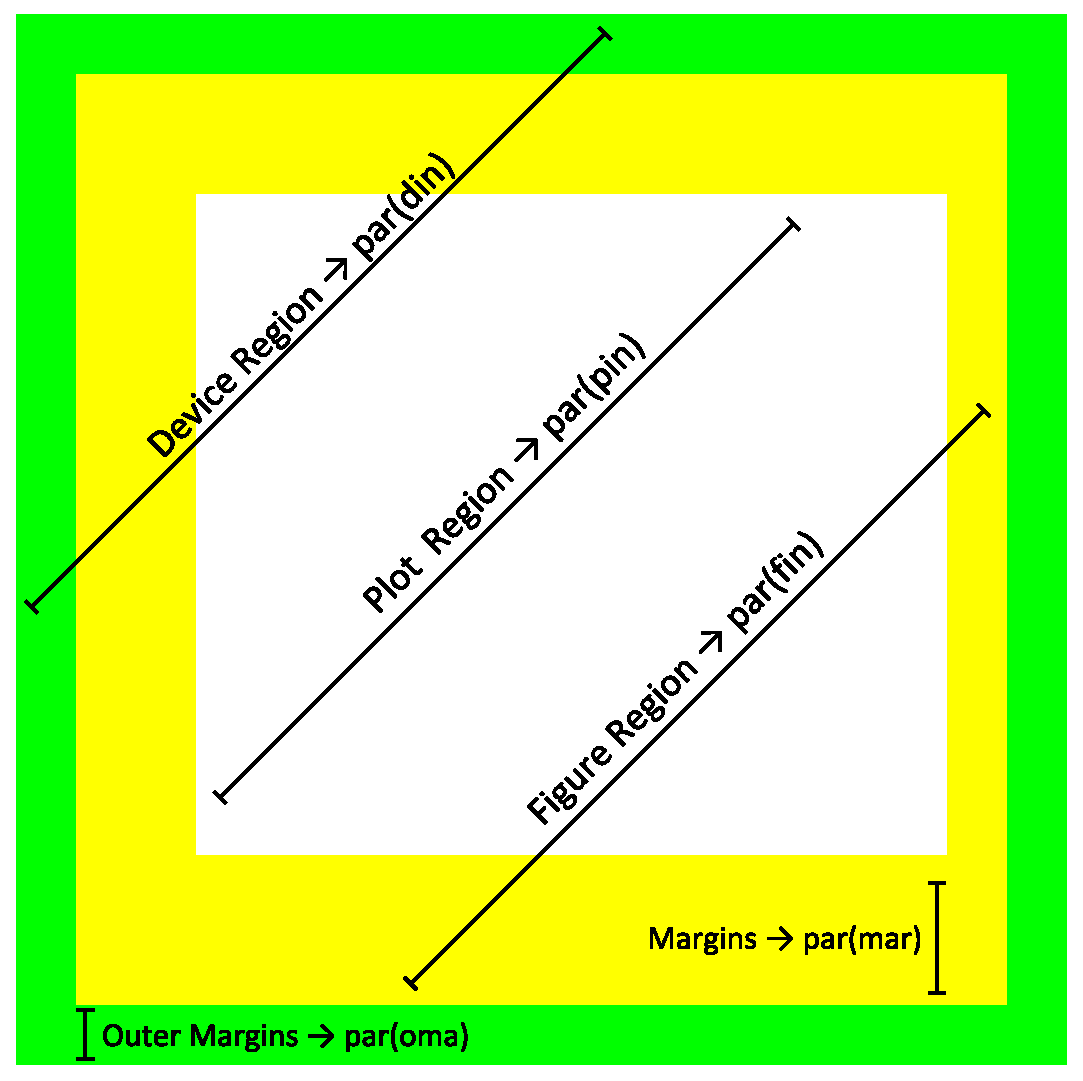
\includegraphics[width=8cm]{devMargins}
\vspace*{-0.5em}
\caption{Regionen und Ränder eines device samt Möglichkeiten, ihre Größe mit \lstinline!par()! ausgeben und ggf.\ verändern zu können (Abschn.\ \ref{sec:par})}
\label{fig:margins}
\end{figure}

\index{Grafik!Fenster öffnen}
\index{Grafik!device!verwalten}
Sofern noch kein Grafikfenster existiert, öffnet es sich mit Eingabe des ersten\index{Grafik!High-Level-Funktion} High-Level-Grafikbefehls automatisch -- in RStudio im \emph{Plots} Tab. In dieses Fenster werden dann alle weiteren Ausgaben grafischer Funktionen hinein gezeichnet, wobei im Fall von High-Level-Funktionen ein ggf.\ bereits vorhandener Inhalt gelöscht wird. Soll für die Ausgabe einer Grafikfunktion zusätzlich zu bereits bestehenden ein neues, zunächst leeres Fenster geöffnet werden, geschieht dies unter Windows mit\index[func]{windows()@\lstinline{windows()}}
\begin{lstlisting}
windows(width=<<Breite>>, height=<<Höhe>>)
\end{lstlisting}

Unter MacOS ist\index[func]{quartz()@\lstinline{quartz()}} \lstinline!quartz()! und unter Unix/Linux\index[func]{x11()@\lstinline{x11()}} \lstinline!x11()! der äquivalente Befehl. Unabhängig vom Betriebssystem erzielt \index[func]{dev.new()@\lstinline{dev.new()}} \lstinline!dev.new()! in der Voreinstellung denselben Effekt. Breite und Höhe des Fensters können über die Argumente \lstinline!width! und \lstinline!height! in der Einheit inch bestimmt werden. Bei mehreren geöffneten devices sind alle bis auf eines inaktiv, das im Fenstertitel die Bezeichnung \emph{(ACTIVE)} trägt. Die Bezeichnung bedeutet, dass in dieses device die Ausgabe der folgenden Grafikfunktion gezeichnet wird, während die Inhalte der anderen devices unverändert bleiben. Um sich einen Überblick über alle aktuell geöffneten devices zu verschaffen, dient der Befehl\index[func]{dev.list()@\lstinline{dev.list()}} \lstinline!dev.list()!.
\begin{lstlisting}
> dev.new(); dev.new(); dev.new()
> dev.list()
windows  windows  windows
      2        3        4
\end{lstlisting}

Die Ausgabe zeigt, welche Ausgabekanäle offen sind. Jedes device besitzt dafür eine laufende Nummer, wobei das erste device die $2$ erhält. Um zu erfahren, welcher der Ausgabekanäle aktiv ist, dient\index[func]{dev.cur()@\lstinline{dev.cur()}} \lstinline!dev.cur()! (\emph{device current}).
\begin{lstlisting}
> dev.cur()
windows
      4
\end{lstlisting}

\index{Grafik!device!verwalten}
Die Ausgabe besteht in der fortlaufenden Nummer des aktiven device. \lstinline!dev.prev()!\index[func]{dev.prev()@\lstinline{dev.prev()}} (\emph{device previous}) und\index[func]{dev.next()@\lstinline{dev.next()}} \lstinline!dev.next()! geben bei mehreren geöffneten devices die Nummer desjenigen device zurück, das sich unmittelbar vor bzw.\ unmittelbar hinter dem aktiven device befindet. Diese Information kann etwa zum Wechseln des aktiven device mit\index[func]{dev.set()@\lstinline{dev.set()}} \lstinline!dev.set(<<Nummer>>)! verwendet werden, damit die Ausgabe der folgenden Grafikfunktionen dort erfolgt.
\begin{lstlisting}
> dev.set(3)                            # aktiviere device 3
windows
      3

> dev.set(dev.next())                   # aktiviere das folgende device
windows
      4
\end{lstlisting}

\index{Grafik!device!verwalten}
Das aktive device wird mit\index[func]{dev.off()@\lstinline{dev.off()}} \lstinline!dev.off()! geschlossen. Handelt es sich um ein Grafikfenster, hat dies denselben Effekt, wie das Fenster per Mausklick zu schließen. Die Ausgabe von \lstinline!dev.off()! gibt an, welches fortan das aktive device ist. Ohne weitere geöffnete devices ist dies das \emph{NULL}-device mit der Nummer $1$. Alle offenen devices lassen sich gleichzeitig mit \lstinline!graphics.off()!\index[func]{graphics.off()@\lstinline{graphics.off()}} schließen.
\begin{lstlisting}
> dev.off()                             # aktuelles device schließen
windows
      2

> graphics.off()                        # alle devices schließen
\end{lstlisting}

%%%%%%%%%%%%%%%%%%%%%%%%%%%%%%%%%%%%%%%%%%%%%%%%%%%%%%%%%%%%%%%%%%
%%%%%%%%%%%%%%%%%%%%%%%%%%%%%%%%%%%%%%%%%%%%%%%%%%%%%%%%%%%%%%%%%%
\subsection{Grafiken speichern}
\label{sec:saveDiag}
%%%%%%%%%%%%%%%%%%%%%%%%%%%%%%%%%%%%%%%%%%%%%%%%%%%%%%%%%%%%%%%%%%
%%%%%%%%%%%%%%%%%%%%%%%%%%%%%%%%%%%%%%%%%%%%%%%%%%%%%%%%%%%%%%%%%%

\index{Grafik!speichern}
Alles, was sich in einem Grafikfenster anzeigen lässt, kann auch als Datei gespeichert werden -- in RStudio im \emph{Plots}-Tab mit dem Eintrag \emph{Export}. Ist ein Grafikfenster aktiviert, so ändert sich das Menü der R-Umgebung dahingehend, dass über \emph{Datei: Speichern als:} die Grafik in vielen Formaten gespeichert werden kann. Als Alternative erlaubt ein sich durch Rechtsklick auf das Grafikfenster öffnendes Kontextmenü, die Grafik in wenigen Formaten zu speichern. Dasselbe Kontextmenü enthält auch Einträge, um die Grafik in einem bestimmten Format in die Zwischenablage zu kopieren und so direkt anderen Programmen verfügbar zu machen.

Grafiken lassen sich auch befehlsgesteuert ohne den Umweg eines Grafikfensters in Dateien speichern. Unabhängig davon, in welchem Format dies geschehen soll, sind dafür drei Arbeitsschritte notwendig: Zunächst muss die Datei als Ausgabekanal (also als aktives device) festgelegt werden. Dazu dient etwa\index[func]{pdf()@\lstinline{pdf()}} \lstinline!pdf()!, wenn die Grafik im PDF-Format zu speichern ist. Es folgen Befehle zum Erstellen von Diagrammen oder Einfügen von Grafikelementen, deren Ausgabe dann nicht auf dem Bildschirm erscheint, sondern direkt in die Datei umgeleitet wird. Schließlich ist der Befehl \lstinline!dev.off()! oder \lstinline!graphics.off()! notwendig, um die Ausgabe in die Datei zu beenden und das device zu schließen.

\index{Grafik!Formate}
Als Dateiformate stehen viele der üblichen bereit, vgl.\ \lstinline!?device! für eine Aufstellung. Beispielhaft seien hier \lstinline!pdf()! und \lstinline!jpeg()! \index[func]{jpeg()@\lstinline{jpeg()}} betrachtet.\footnote{Alternativ stellt das Paket\index[pack]{Cairo@\lstinline{Cairo}} \lstinline!Cairo! \cite{Urbanek2014} die gleichnamige Funktion\index[func]{Cairo()@\lstinline{Cairo()}} zur Verfügung, mit der Diagramme in vielen Dateiformaten auch in hoher Auflösung und mit automatischer Kantenglättung gespeichert werden können.}
\begin{lstlisting}
pdf(file="<<Dateiname>>", width=<<Breite>>, height=<<Höhe>>)
jpeg(filename="<<Dateiname>>", width=<<Breite>>, height=<<Höhe>>,
     units="px", quality=<<Bildqualität>>)
\end{lstlisting}

Unter \lstinline!file! bzw.\ \lstinline!filename! ist der Name der Ausgabedatei einzutragen -- ggf.\ inkl.\ einer Pfadangabe (Abschn.\ \ref{sec:files}). Sollen mehrere Grafiken mit gleichem Namensschema unter Zuhilfenahme einer fortlaufenden Nummer erzeugt werden, ist ein spezielles Namensformat zu verwenden, das in der Hilfe erläutert wird. Mit \lstinline!width! und \lstinline!height! wird die Größe der Grafik kontrolliert. Beide Angaben sind bei \lstinline!pdf()! in der Einheit inch zu tätigen, während bei \lstinline!jpeg()! über das Argument \lstinline!units! festgelegt werden kann, auf welche Maßeinheit sie sich beziehen. Voreinstellung ist die Anzahl der pixel, als Alternativen stehen \lstinline!in! (inch), \lstinline!cm! und \lstinline!mm! zur Auswahl. Schließlich kann bei Bildern im JPEG-Format festgelegt werden, wie stark die Daten komprimiert werden sollen, wobei die Kompression mit einem Verlust an Bildinformationen verbunden ist. Das Argument \lstinline!quality! erwartet einen sich auf die höchstmögliche Bildqualität beziehenden Prozentwert -- ein kleinerer Wert bedeutet hier eine geringere Bildqualität, die dann stärkere Kompression führt dafür aber auch zu einer geringeren Dateigröße.

Hier soll demonstriert werden, wie eine einfache Grafik im PDF-Format gespeichert wird.
\begin{lstlisting}
> pdf("pdf_test.pdf")                  # device öffnen (mit Dateinamen)
> plot(1:10, rnorm(10))                # Grafik einzeichnen
> dev.off()                            # device schließen
\end{lstlisting}

%\index{Grafik!kopieren}
%Die Inhalte eines aktiven device können durch\index[func]{dev.copy()@\lstinline{dev.copy()}} \lstinline!dev.copy()! in ein neues device kopiert werden. Dabei ist entweder die Nummer des bereits geöffneten Ziel-Device zu nennen oder anzugeben, welche Art von device mit den bestehenden Inhalten neu geöffnet werden soll.
%\begin{lstlisting}
%> dev.copy(device=<<Device-Typ>>, ..., which=<<Device-Nummer>>)
%\end{lstlisting}
%
%Ist das Ziel-Device noch nicht geöffnet, findet das \lstinline!device! Argument Verwendung, das (ohne Anführungszeichen) den Namen einer Funktion erwartet, mit der ein device eines bestimmten Typs geöffnet werden kann, etwa \lstinline!pdf!. Andernfalls gibt \lstinline!which! die Nummer des geöffneten Ziel-Device an. Benötigt das neu zu erstellende device seinerseits Argumente -- etwa Dateinamen oder Angaben zur Größe der Grafik, so können diese anstelle der \lstinline!...! durch Komma getrennt genannt werden.
%\begin{lstlisting}
%> plot(1:10, rnorm(10))                # Grafikfenster + Diagramm öffnen
%
%# Inhalt des Fensters in JPEG-Bild speichern,
%# dabei Dateinamen und Kompressionsgrad angeben
%> dev.copy(jpeg, filename="copied.jpg", quality=90)
%> graphics.off()                       # beide offenen devices schließen
%\end{lstlisting}

%%%%%%%%%%%%%%%%%%%%%%%%%%%%%%%%%%%%%%%%%%%%%%%%%%%%%%%%%%%%%%%%%%
%%%%%%%%%%%%%%%%%%%%%%%%%%%%%%%%%%%%%%%%%%%%%%%%%%%%%%%%%%%%%%%%%%
\section{Streu- und Liniendiagramme}
\label{sec:plot}
%%%%%%%%%%%%%%%%%%%%%%%%%%%%%%%%%%%%%%%%%%%%%%%%%%%%%%%%%%%%%%%%%%
%%%%%%%%%%%%%%%%%%%%%%%%%%%%%%%%%%%%%%%%%%%%%%%%%%%%%%%%%%%%%%%%%%

\index{Grafik!Streudiagramm}
In zweidimensionalen Streudiagrammen (\emph{scatterplots}) werden mit \lstinline!plot()! Wertepaare in Form von Punkten in einem kartesischen Koordinatensystem dargestellt, wobei ein Wert die Position des Punkts entlang der Abszisse ($x$-Achse) und der andere Wert die Position des Punkts entlang der Ordinate ($y$-Achse) bestimmt. Die Punkte können dabei für ein Liniendiagramm durch Linien verbunden oder für ein Streudiagramm als Punktwolke belassen werden.

%%%%%%%%%%%%%%%%%%%%%%%%%%%%%%%%%%%%%%%%%%%%%%%%%%%%%%%%%%%%%%%%%%
%%%%%%%%%%%%%%%%%%%%%%%%%%%%%%%%%%%%%%%%%%%%%%%%%%%%%%%%%%%%%%%%%%
\subsection{Streudiagramme mit \texttt{plot()}}
%%%%%%%%%%%%%%%%%%%%%%%%%%%%%%%%%%%%%%%%%%%%%%%%%%%%%%%%%%%%%%%%%%
%%%%%%%%%%%%%%%%%%%%%%%%%%%%%%%%%%%%%%%%%%%%%%%%%%%%%%%%%%%%%%%%%%

\index[func]{plot()@\lstinline{plot()}|textbf}
\index{Grafik!Liniendiagramm}
\begin{lstlisting}
plot(x=<<Vektor>>, y=<<Vektor>>, type="<<Option>>", main="<<Diagrammtitel>>",
     sub="<<Untertitel>>", asp=<<Seitenverhältnis Höhe/Breite>>)
\end{lstlisting}

Unter \lstinline!x! und \lstinline!y! sind die $x$- bzw.\ $y$-Koordinaten der Punkte jeweils als Vektor einzutragen. Wird nur ein Vektor angegeben, werden seine Werte als $y$-Koordinaten interpretiert und die $x$-Koordinaten durch die Indizes des Vektors gebildet.\footnote{Dagegen erzeugt \lstinline!plot(<<Faktor>>, ...)! ein Säulendiagramm der Häufigkeiten jeder Faktorstufe (Abschn.\ \ref{sec:barplot}), da \lstinline!plot()! eine generische Funktion ist (Abschn.\ \ref{sec:funcGeneric}).} Das Argument \lstinline!type! hat mehrere mögliche Ausprägungen, die das Aussehen der Datenmarkierungen im Diagramm bestimmen (Tab.\ \ref{tab:plotArgs}, Abb.\ \ref{fig:plotTypes}). Der Diagrammtitel kann als Zeichenkette für \lstinline!main! angegeben werden, der Untertitel für \lstinline!sub!. Das Verhältnis von Höhe zu Breite jeweils einer Skaleneinheit im Diagramm kontrolliert das Argument \lstinline!asp! (\emph{aspect ratio}), für weitere Argumente vgl.\ \lstinline!?plot.default!.

Die Koordinaten der Punkte können auch über andere Wege angegeben werden: Als Modellformel lautet der Aufruf \lstinline!plot(<<y-Koord.>> ~ <<x-Koord.>>, data=<<Datensatz>>)!.\footnote{Hat die Modellformel die Form \lstinline!<<y-Koord.>> ~ <<Faktor>>!, werden in einem Diagramm getrennt für die von \lstinline!<<Faktor>>! definierten Gruppen boxplots dargestellt (Abschn.\ \ref{sec:boxplot}).} Wenn die in der Modellformel verwendeten Variablen aus einem Datensatz stammen, ist dieser unter \lstinline!data! zu nennen. Weiter ist es möglich, eine Liste mit zwei Komponenten \lstinline!x! und \lstinline!y! anzugeben, die die Koordinaten enthalten. Schließlich kann einfach eine Matrix mit zwei Spalten für die $(x, y)$-Koordinaten übergeben werden.

%\begin{longtable}{p{2.3cm}p{9.5cm}}
\begin{table}[ht]
\centering
\caption{Mögliche Werte für das Argument \lstinline!type! von \lstinline!plot()!}
\label{tab:plotArgs}
\begin{tabular}{p{2.3cm}p{10.2cm}}
\hline
\sffamily Wert für \lstinline!type! & \sffamily Bedeutung\\\hline\hline
\lstinline!"p"! & Punkte\\
\lstinline!"l"! & durchgehende Linien. Durch eng gesetzte Stützstellen können Funktionskurven beliebiger Form approximiert werden\\
\lstinline!"b"! & Punkte und Linien\\
\lstinline!"c"! & unterbrochene Linien\\
\lstinline!"o"! & Punkte und Linien, aber überlappend\\
\lstinline!"h"! & senkrechte Linien zu jedem Datenpunkt (\emph{spike plot})\\
\lstinline!"s"! & Stufendiagramm\\
\lstinline!"S"! & Stufendiagramm mit anderer Reihenfolge von vertikalen und horizontalen Schritten zur nächsten Stufe\\
\lstinline!"n"! & fügt dem Diagramm keine Datenpunkte hinzu (\emph{no plotting})\\\hline
\end{tabular}
\end{table}
%\end{longtable}

\begin{lstlisting}
> vec <- rnorm(10)                            # Daten

# das Argument xlab=NA entfernt die Bezeichnung der x-Achse
> plot(vec, type="p", xlab=NA, main="type p")
> plot(vec, type="l", xlab=NA, main="type l")
> plot(vec, type="b", xlab=NA, main="type b")
> plot(vec, type="o", xlab=NA, main="type o")
> plot(vec, type="s", xlab=NA, main="type s")
> plot(vec, type="h", xlab=NA, main="type h")
\end{lstlisting}

\begin{figure}[ht]
\centering
\includegraphics[width=12.5cm]{plotTypes}
\vspace*{-1em}
\caption{Mit \lstinline!plot(type="<<Option>>")! erzeugbare Diagrammarten}
\label{fig:plotTypes}
\end{figure}

%%%%%%%%%%%%%%%%%%%%%%%%%%%%%%%%%%%%%%%%%%%%%%%%%%%%%%%%%%%%%%%%%%
%%%%%%%%%%%%%%%%%%%%%%%%%%%%%%%%%%%%%%%%%%%%%%%%%%%%%%%%%%%%%%%%%%
\subsection{Datenpunkte eines Streudiagramms identifizieren}
%%%%%%%%%%%%%%%%%%%%%%%%%%%%%%%%%%%%%%%%%%%%%%%%%%%%%%%%%%%%%%%%%%
%%%%%%%%%%%%%%%%%%%%%%%%%%%%%%%%%%%%%%%%%%%%%%%%%%%%%%%%%%%%%%%%%%

\index{Grafik!Datenpunkte identifizieren}
Werden viele Daten in einem Streudiagramm dargestellt, ist häufig nicht ersichtlich, zu welchem Wert ein bestimmter Datenpunkt gehört. Diese Information kann jedoch interessant sein, wenn etwa erst die grafische Betrachtung eines Datensatzes Besonderheiten der Verteilung verrät und die für bestimmte Datenpunkte verantwortlichen Untersuchungseinheiten identifiziert werden sollen. \lstinline!identify()!\index[func]{identify()@\lstinline{identify()}} erlaubt es, Werte in einem Streudiagramm interaktiv zu identifizieren.
\begin{lstlisting}
identify(x=<<x-Koordinaten>>, y=<<y-Koordinaten>>)
\end{lstlisting}

Für \lstinline!x! und \lstinline!y! sollten dieselben Daten in Form von Vektoren mit $x$- und $y$-Koordinaten übergeben werden, die zuvor in einem noch geöffneten Grafikfenster als Streudiagramm dargestellt wurden. Wird nur ein Vektor angegeben, werden seine Werte als $y$-Koordinaten interpretiert und die $x$-Koordinaten durch die Indizes des Vektors gebildet. Durch Ausführen von \lstinline!identify()! ändert sich der Mauszeiger über der Diagrammfläche zu einem Kreuz. Mit einem Klick der linken Maustaste wird derjenige Datenpunkt identifiziert, der der Mausposition am nächsten liegt und sein Index dem Diagramm neben dem Datenpunkt hinzugefügt. Die Konsole ist in dieser Zeit blockiert. Der Vorgang kann mehrfach wiederholt und schließlich durch Klicken der rechten Maustaste über ein Kontextmenü beendet werden, woraufhin \lstinline!identify()! die Indizes der ausgemachten Punkte zurückgibt. In RStudio wird der Vorgang durch Drücken der \lstinline[language=]!ESC! Taste beendet.
\begin{lstlisting}
> vec <- rnorm(10)
> plot(vec)
> identify(vec)
# Mausclicks ...
[1] 1 4 5 8
\end{lstlisting}

%%%%%%%%%%%%%%%%%%%%%%%%%%%%%%%%%%%%%%%%%%%%%%%%%%%%%%%%%%%%%%%%%%
%%%%%%%%%%%%%%%%%%%%%%%%%%%%%%%%%%%%%%%%%%%%%%%%%%%%%%%%%%%%%%%%%%
\subsection{Streudiagramme mit \texttt{matplot()}}
%%%%%%%%%%%%%%%%%%%%%%%%%%%%%%%%%%%%%%%%%%%%%%%%%%%%%%%%%%%%%%%%%%
%%%%%%%%%%%%%%%%%%%%%%%%%%%%%%%%%%%%%%%%%%%%%%%%%%%%%%%%%%%%%%%%%%

\index{Grafik!Streudiagramm}
\index{Grafik!Liniendiagramm}
\index{Streudiagramm|see{Grafik}}
So wie durch \lstinline!plot()! ein Streudiagramm einer einzelnen Datenreihe erstellt wird, erzeugt \lstinline!matplot()! ein Streudiagramm für mehrere Datenreihen gleichzeitig\index[func]{matplot()@\lstinline{matplot()}} (Abb.\ \ref{fig:matplot}).
\begin{lstlisting}
matplot(x=<<Matrix>>, y=<<Matrix>>, type="<<Option>>", pch="<<Symbol>>")
\end{lstlisting}

Die Argumente sind dieselben wie für \lstinline!plot()!, lediglich $x$- und $y$-Koordinaten können nun als Matrizen an \lstinline!x! und \lstinline!y! übergeben werden. Dabei wird jede ihrer Spalten als eine separate Datenreihe interpretiert. Haben dabei alle Datenreihen dieselben $x$-Koordinaten, kann \lstinline!x! auch ein Vektor sein. Wird nur eine Matrix mit Koordinaten angegeben, werden diese als $y$-Koordinaten gedeutet und die $x$-Koordinaten durch die Zeilenindizes der Werte gebildet. In der Voreinstellung werden die Datenreihen in unterschiedlichen Farben dargestellt. Als Symbol für jeden Datenpunkt dienen die Ziffern 1--9, die mit der zur Datenreihe gehörenden Spaltennummer korrespondieren. Mit dem Argument \lstinline!pch! können auch andere Symbole Verwendung finden (Abschn.\ \ref{sec:par}, Abb. \ref{fig:pchLty}).
\begin{lstlisting}
> vec <- seq(from=-2*pi, to=2*pi, length.out=50)
> mat <- cbind(2*sin(vec), sin(vec-(pi/4)), 0.5*sin(vec-(pi/2)))
> matplot(vec, mat, type="b", xlab=NA, ylab=NA, pch=1:3,
+         main="Sinuskurven")
\end{lstlisting}

\begin{figure}[ht]
\centering
\includegraphics[width=8cm]{matplot}
\vspace*{-1.5em}
\caption{Mit \lstinline!matplot()! erzeugtes Streudiagramm}
\label{fig:matplot}
\end{figure}

%%%%%%%%%%%%%%%%%%%%%%%%%%%%%%%%%%%%%%%%%%%%%%%%%%%%%%%%%%%%%%%%%%
%%%%%%%%%%%%%%%%%%%%%%%%%%%%%%%%%%%%%%%%%%%%%%%%%%%%%%%%%%%%%%%%%%
\section{Diagramme formatieren}
\label{sec:graphFormat}
%%%%%%%%%%%%%%%%%%%%%%%%%%%%%%%%%%%%%%%%%%%%%%%%%%%%%%%%%%%%%%%%%%
%%%%%%%%%%%%%%%%%%%%%%%%%%%%%%%%%%%%%%%%%%%%%%%%%%%%%%%%%%%%%%%%%%

\lstinline!plot()! akzeptiert wie auch andere High-Level-Grafikfunktionen eine Vielzahl weiterer Argumente, mit denen ein Diagramm flexibel angepasst werden kann. Einige der wichtigsten Möglichkeiten zur individuellen Gestaltung werden im Folgenden vorgestellt.

%%%%%%%%%%%%%%%%%%%%%%%%%%%%%%%%%%%%%%%%%%%%%%%%%%%%%%%%%%%%%%%%%%
%%%%%%%%%%%%%%%%%%%%%%%%%%%%%%%%%%%%%%%%%%%%%%%%%%%%%%%%%%%%%%%%%%
\subsection{Grafikelemente formatieren}
\label{sec:par}
%%%%%%%%%%%%%%%%%%%%%%%%%%%%%%%%%%%%%%%%%%%%%%%%%%%%%%%%%%%%%%%%%%
%%%%%%%%%%%%%%%%%%%%%%%%%%%%%%%%%%%%%%%%%%%%%%%%%%%%%%%%%%%%%%%%%%

\index{Grafik!formatieren}
\index{Grafik!Optionen}
\index{Grafik!Einstellungen}
Die Formatierung von Grafikelementen ist in vielen Aspekten variabel, etwa hinsichtlich der Art, Größe und Farbe der verwendeten Symbole oder der Orientierung der Achsenbeschriftungen. Zu diesem Zweck akzeptieren die meisten High-Level-Funktionen einen gemeinsamen Satz zusätzlicher Argumente, auch wenn diese nicht immer in den jeweiligen Hilfe-Seiten mit aufgeführt sind. Die gebräuchlichsten von ihnen sind in Tab.\ \ref{tab:parArgsBoth} beschrieben.

\begin{longtable}{p{1.5cm}p{3.2cm}p{7.8cm}}
%\begin{table}[ht]
%\centering
%\begin{tabular}{p{1.8cm}p{3.2cm}p{9cm}}
\caption{Diagrammoptionen, die in \lstinline!par()! und high-level Grafik-Funktionen gesetzt werden können
\label{tab:parArgsBoth}}\\
\endfirsthead
\caption[]{(Forts.)}\\\hline
\endhead
\hline
\sffamily Argument & \sffamily Wert & \sffamily Bedeutung\\\hline\hline
\lstinline!bty! & \lstinline!"o"!, \lstinline!"n"! & Bei \lstinline!"o"! wird ein Rahmen um die die Datenpunkte enthaltende Plot-Region gezogen, bei \lstinline!"n"! nicht\\
\lstinline!cex! & \lstinline!<<Zahl>>! & Vergrößerungsfaktor für die Datenpunkt-Symbole. Voreinstellung ist der Wert $1$\\
\lstinline!cex.axis! & \lstinline!<<Zahl>>! & Vergrößerungsfaktor für die Achsenbeschriftungen. Voreinstellung ist der Wert $1$\\
\lstinline!cex.lab! & \lstinline!<<Zahl>>! & Vergrößerungsfaktor für die Schrift der Achsenbezeichnungen. Voreinstellung ist der Wert $1$\\
\lstinline!col! & \lstinline!"<<Farbe>>"! & Farbe der Datenpunkt-Symbole sowie bei \lstinline!par()! zusätzlich des Rahmens um die Plot-Region (s.\ Abschn.\ \ref{sec:colors} für mögliche Werte)\\
\lstinline!las! & \lstinline!0!, \lstinline!1!, \lstinline!2!, \lstinline!3! & Orientierung der Achsenbeschriftungen. Für senkrecht zur Achse stehende Beschriftungen ist der Wert auf $2$ zu setzen\\
\lstinline!lty! & \lstinline!1!, \lstinline!2!, \lstinline!3!, \lstinline!4!, \lstinline!5!, \lstinline!6! bzw.\ \lstinline!<<Schlüsselwort>>! & Linientyp: Schlüsselwörter sind \lstinline!"solid"!, \lstinline!"dashed"!, \lstinline[breaklines=false]!"dotted"!, \lstinline!"dotdash"!, \lstinline!"longdash"!, \lstinline!"twodash"! (Abb.\ \ref{fig:pchLty})\\
\lstinline!lwd! & \lstinline!<<Zahl>>! & Linienstärke, auch bei Datenpunktsymbolen. Voreinstellung ist der Wert $1$.\\
\lstinline!pch! & \lstinline!<<Zahl 1-25>>! bzw.\ \lstinline[breaklines=false]!"<<Buchstabe>>"! & Art der Datenpunkt-Symbole. Dabei steht etwa $16$ für den ausgefüllten Punkt. Für andere Werte vgl.\ \lstinline!?points! und Abb.\ \ref{fig:pchLty}. Wird ein Buchstabe angegeben, dient dieser als Symbol der Datenpunkte\\
\lstinline!xpd! & \lstinline!NA!, \lstinline!TRUE!, \lstinline!FAlSE! & Grafikelemente können nur in der Plot-Region eingefügt werden (Voreinstellung \lstinline!FALSE!: clipping\index{Grafik!clipping}). \lstinline!TRUE!: gesamte Figure-Region steht zur Verfügung, \lstinline!NA!: gesamte Device-Region (Abschn.\ \ref{sec:device}, \ref{sec:clipping})\\\hline
%\end{tabular}
%\end{table}
\end{longtable}

Anstatt die in Tab.\ \ref{tab:parArgsBoth} genannten Argumente direkt beim Aufruf von Grafikfunktionen mit anzugeben, können sie durch die separate Funktion\index[func]{par()@\lstinline{par()}} \lstinline!par(<<Option>>=<<Wert>>)! festgelegt werden. \lstinline!par()! kann darüber hinaus noch weitere Einstellungen ändern, die in Tab.\ \ref{tab:parArgsPar} aufgeführt sind. Die aktuell für das aktive device gültigen Einstellungen lassen sich durch \lstinline!par("<<Opt1>>", "<<Opt2>>", ...)! als Liste ausgeben, d.\,h.\ durch Nennung der relevanten Argumente ohne Zuweisung von Werten. Ohne weitere Argumente gibt \lstinline!par()! die aktuellen Werte für alle veränderbaren Parameter aus.

\begin{table}[ht]
\centering
\caption{Grafikoptionen, die nur über \lstinline!par()! verändert werden können}
\label{tab:parArgsPar}
\begin{tabular}{p{1.5cm}p{1.6cm}p{9.4cm}}
\hline
\sffamily Argument & \sffamily Wert & \sffamily Bedeutung\\\hline\hline
\lstinline!mar! & \lstinline!<<Vektor>>! & Ränder zwischen Plot- und Figure-Region eines Diagramms (Abb.\ \ref{fig:margins}). Angabe als Vielfaches der Zeilenhöhe in Form eines Vektor mit vier Elementen, die jeweils dem unteren, linken, oberen und rechten Rand entsprechen. Voreinstellung ist \lstinline!c(5, 4, 4, 2)!\\
\lstinline!mai! & \lstinline!<<Vektor>>! & Wie \lstinline!mar!, jedoch in der Einheit inch\\
\lstinline!oma! & \lstinline!<<Vektor>>! & Ränder zwischen Figure- und Device-Region einer Grafik (Abb.\ \ref{fig:margins}). Bei aufgeteilten Diagrammen zwischen den zusammengefassten Figure-Regionen und der Device-Region. Angabe wie bei \lstinline!mar!. Voreinstellung ist \lstinline!c(0, 0, 0, 0)!, d.\,h.\ die Figure-Region füllt die Device-Region vollständig aus\\
\lstinline!omi! & \lstinline!<<Vektor>>! & Wie \lstinline!oma!, jedoch in der Einheit inch\\\hline
\end{tabular}
\end{table}

Die mit \lstinline!par()! geänderten Parameter sind Einstellungen für das aktive device. Sie gelten für alle folgenden Ausgaben in dieses device bis zur nächsten expliziten Änderung, oder bis ein neues device aktiviert wird. Der auf der Konsole nicht sichtbare Rückgabewert von \lstinline!par()! enthält die alten Einstellungen der geänderten Optionen in Form einer Liste, die auch direkt wieder an \lstinline!par()! übergeben werden kann. Auf diese Weise lassen sich Einstellungen temporär ändern und dann wieder auf den Ursprungswert zurücksetzen (Abb.\ \ref{fig:par}).
\begin{lstlisting}
# Werte ändern und alte speichern
> op <- par(col="gray60", lwd=2, pch=16)
> plot(rnorm(10), main="Grau, fett, gefüllte Kreise")

# Parameter auf ursprüngliche Werte zurücksetzen
> par(op)
> plot(rnorm(10), main="Standardformatierung")
\end{lstlisting}

\begin{figure}[ht]
\centering
\includegraphics[width=12.5cm]{par}
\vspace*{-1em}
\caption{Verwendung von \lstinline!par()! zur Diagrammformatierung}
\label{fig:par}
\end{figure}

\index{Grafik!Linientypen}
\index{Grafik!Datenpunktsymbole}
Abbildung \ref{fig:pchLty} veranschaulicht die mit \lstinline!lty! und \lstinline!pch! einstellbaren Linientypen und Datenpunkt-Symbole (s.\ Abschn.\ \ref{sec:graphAddElem} für das Einfügen von Elementen in ein Diagramm). Symbole $21$--$25$ sind ausgefüllte Datenpunkte, deren Füllfarbe in Zeichenfunktionen über das Argument \lstinline!bg="<<Farbe>>"! definiert wird, während \lstinline!col="<<Farbe>>"! die Farbe des Randes bezeichnet (Abschn.\ \ref{sec:colors}).
\begin{lstlisting}
# Koordinaten der Datenpunkte
> X <- row(matrix(numeric(6*11), nrow=6, ncol=11))
> Y <- col(matrix(numeric(6*11), nrow=6, ncol=11))

# leeres Diagramm mit der richtigen Skalierung
> plot(0:6, seq(1, 11, length.out=7), type="n", axes=FALSE,
+      main="pch Datenpunkt-Symbole und lty Linientypen")

# Symbole für pch mit grauem Hintergrund für 21-25
> points(X[1:26], Y[1:26], pch=0:25, bg="gray", cex=2)

# Linien für lty
> matlines(X[ , 6:11], Y[ , 6:11], lty=6:1, lwd=2, col="black")

# erklärender Text - Nummer der pch Symbole und lty Linientypen
> text(X[1:26]-0.3, Y[1:26],    labels=0:25)
> text(rep(0.7, 6), Y[1, 6:11], labels=6:1)
> text(0, 9, labels="Linientypen für lty", srt=90, cex=1.2)
> text(0, 3, labels="Symbole für pch",     srt=90, cex=1.2)
\end{lstlisting}

\begin{figure}[ht]
\centering
\includegraphics[width=8cm]{pchLty}
\vspace*{-1em}
\caption{Datenpunkt-Symbole und Linientypen zur Verwendung für die Argumente \lstinline!pch! und \lstinline!lty! von Grafikfunktionen}
\label{fig:pchLty}
\end{figure}

%%%%%%%%%%%%%%%%%%%%%%%%%%%%%%%%%%%%%%%%%%%%%%%%%%%%%%%%%%%%%%%%%%
%%%%%%%%%%%%%%%%%%%%%%%%%%%%%%%%%%%%%%%%%%%%%%%%%%%%%%%%%%%%%%%%%%
\subsection{Farben spezifizieren}
\label{sec:colors}
%%%%%%%%%%%%%%%%%%%%%%%%%%%%%%%%%%%%%%%%%%%%%%%%%%%%%%%%%%%%%%%%%%
%%%%%%%%%%%%%%%%%%%%%%%%%%%%%%%%%%%%%%%%%%%%%%%%%%%%%%%%%%%%%%%%%%

\index{Grafik!Farben}
\index{Farben|see{Grafik}}
Häufig ist es sinnvoll, Diagrammelemente farblich hervorzuheben, etwa um die Zusammengehörigkeit von Punkten innerhalb von Datenreihen zu kennzeichnen und verschiedene Datenreihen leichter voneinander unterscheidbar zu machen. Auch Text- und Hintergrundfarben können in Diagrammen frei gewählt werden. Zu diesem Zweck lassen sich Farben in unterschiedlicher Form an die entsprechenden Funktionsargumente (meist \lstinline!col!) übergeben:

\begin{itemize}
\item Als Farbname, z.\,B.\ \lstinline!"green"! oder \lstinline!"blue"!, vgl.\ \lstinline!colors()!\index[func]{colors()@\lstinline{colors()}} für mögliche Werte.
\item Im Hexadezimalformat, wobei die Intensitäten der Monitor-Grundfarben Rot, Grün und Blau in der Form \lstinline!"#RRGGBB"! mit Werten für \lstinline!RR!, \lstinline!GG! und \lstinline!BB! im Bereich von \lstinline!00! bis \lstinline!FF! angegeben werden. \lstinline!"#FF0000"! entspräche Rot, \lstinline!"#00FF00"! Grün.
\item Als natürliche Zahl, die als Index für die derzeit aktive Farbpalette interpretiert wird. Eine Farbpalette ist dabei ein vordefinierter Vektor von Farben, der mit\index[func]{palette()@\lstinline{palette()}} \lstinline!palette()! ausgegeben werden kann. Die voreingestellte Palette beginnt mit den Farben \lstinline!"black"!, \lstinline!"#DF536B"!, \lstinline!"#61D04F"!, -- der Index \lstinline!2! entspräche einem entsättigten Rot. Die Palette kann gewechselt werden, indem an \lstinline!palette(<<Vektor>>)! ein Vektor mit Farbnamen übergeben wird. Der (auf der Konsole unsichtbare) Rückgabewert enthält die ersetzte Palette und kann für einen temporären Wechsel der Palette in einem Vektor zwischengespeichert und später wieder an \lstinline!palette()! übergeben werden. Alternativ stellt \lstinline!palette("default")! die ursprünglich voreingestellte Palette wieder her. Für eine Beschreibung der verfügbaren Paletten vgl.\ \lstinline!?hcl.colors!. Die dort genannten Funktionen können etwa dazu eingesetzt werden, die aktive Farbpalette zu ändern, indem ihre Ausgabe an \lstinline!palette()! übergeben wird, z.\,B.\ mit \lstinline!palette(hcl.colors(10))!.\footnote{Das Paket \index[pack]{colorspace@\lstinline{colorspace}|textbf} \lstinline!colorspace! \cite{Zeileis2019, Ihaka2009} definiert eine Reihe von Paletten, deren Farben für besonders gute Unterscheidbarkeit unter verschiedenen Randbedingungen optimiert wurden -- etwa für Farbfehlsichtige oder Graustufen-Ausdrucke. Weiterführende Artikel zu diesem Thema nennt \lstinline!vignette("colorspace")!.}
\end{itemize}

\lstinline!col2rgb(<<Farbe>>)!\index[func]{col2rgb()@\lstinline{col2rgb()}} wandelt Farbnamen, Palettenindizes und Farben im Hexadezimalformat in einen Spaltenvektor um, der die Intensitäten der Monitor-Grundfarben Rot, Grün und Blau im Wertebereich von $0$--$255$ enthält. Namen und Hexadezimalzahlen müssen dabei in Anführungszeichen gesetzt werden. Da die Spezifizierung von Farben im Hexadezimalformat nicht sehr intuitiv ist, stellt R verschiedene Funktionen bereit, mit denen Farben auf einfachere Art definiert werden können. Diese Funktionen geben dann die bezeichnete Farbe im Hexadezimalformat aus.

\begin{itemize}
\item Mit\index[func]{rgb()@\lstinline{rgb()}} \lstinline!rgb(red=<<Rot>>, green=<<Grün>>, blue=<<Blau>>)! können die Intensitäten der Monitor-Grundfarben Rot, Grün und Blau mit Zahlen im Wertebereich von $0$--$1$ angegeben werden. Andere Höchstwerte lassen sich über das Argument \lstinline!maxColorValue! festlegen.\footnote{\label{ftn:transp}Ein vierter Wert zwischen $0$ und $1$ kann den Grad des\index{Grafik!Transparenz} \emph{alpha-blendings} für simulierte Transparenz definieren. Niedrige Werte stehen für sehr durchlässige, hohe Werte für opaque Farben (Abb.\ \ref{fig:pca}). Diese Art von Transparenz wird nur von manchen devices unterstützt, etwa von \lstinline!pdf()! oder \lstinline!png()!.} So gibt etwa \lstinline!rgb(0, 1, 1)! die Farbe \lstinline!"#00FFFF"! (Cyan) aus. Bei von \lstinline!col2rgb()! erzeugten Vektoren ist \lstinline!rgb()! mit dem Argument \lstinline!maxColorValue=255! zu verwenden.
\item Analog erzeugt\index[func]{hsv()@\lstinline{hsv()}} \lstinline!hsv(h=<<Farbton>>, s=<<Sättigung>>, v=<<Helligkeit>>)! (\emph{hue, saturation, value}) Farben, die mit Zahlen im Wertebereich von $0$--$1$ für Farbton, Sättigung und Helligkeit definiert werden.\footnote{Für weitere Funktionen zur Verwendung verschiedener Farbräume vgl.\  \index[func]{convertColor()@\lstinline{convertColor()}} \lstinline!?convertColor! sowie das Paket\index[pack]{colorspace@\lstinline{colorspace}} \lstinline!colorspace!.} So entspricht etwa \lstinline!hsv(0.1666, 1, 1)! der Farbe \lstinline!"#FFFF00"! (Gelb). \lstinline!rgb2hsv(r=<<Rot>>, g=<<Grün>>, b=<<Blau>>)!\index[func]{rgb2hsv()@\lstinline{rgb2hsv()}} rechnet von RGB-Farben in HSV-Werte um.
\item \lstinline!hcl(h=<<Farbton>>, c=<<Sättigung>>, l=<<Helligkeit>>)!\index[func]{hcl()@\lstinline{hcl()}} (\emph{hue, chroma, luminance}) erzeugt Farben im CIE Luv Koordinatensystem, das auf gleiche perzeptuelle Unterschiedlichkeit von im Farbraum gleich weit entfernten Farben abzielt. Dabei ist \lstinline!h! ein Winkel im Farbkreis im Bereich von $0$--$360^{\circ}$, \lstinline!c! die Sättigung, deren Höchstwert vom Farbton und der Luminanz abhängt und schließlich \lstinline!l! die Luminanz im Bereich von $0$--$100$.
\item \lstinline!gray(<<Grauwert>>)!\index[func]{gray()@\lstinline{gray()}} akzeptiert eine Zahl im Wertebereich von $0$--$1$, die als Helligkeit einer achromatischen Farbe mit identischen RGB-Werten interpretiert wird. So erzeugt etwa \lstinline!gray(0.5)! die graue Farbe \lstinline!"#808080"!. Das optionale Argument \lstinline!alpha! kontrolliert den Grad simulierter Transparenz (Fußnote \ref{ftn:transp}).
\item \lstinline!colorRamp(<<Farben>>)!\index[func]{colorRamp()@\lstinline{colorRamp()}} und \lstinline!colorRampPalette(<<Farben>>)!\index[func]{colorRampPalette()@\lstinline{colorRampPalette()}} erstellen einen Farbverlauf, indem sie im Farbraum gleichmäßig zwischen den übergebenen Farben interpolieren. Über das Argument \lstinline!alpha=TRUE! gilt dies auch für den Grad simulierter Transparenz. Das Ergebnis von \lstinline!colorRamp()! ist dabei eine Funktion, die ihrerseits eine Zahl im Bereich $[0,1]$ akzeptiert und als relative Distanz zwischen der ersten und letzten zu interpolierenden Farbe interpretiert. Dagegen ist die Ausgabe von \lstinline!colorRampPalette()! eine Funktion, die analog zu den vordefinierten Palettenfunktionen wie \lstinline!rainbow()! oder \lstinline!cm.colors()! arbeitet.
\item Eine gegebene Farbe kann mit \lstinline!adjustcolor()!\index[func]{adjustcolor()@\lstinline{adjustcolor()}} hinsichtlich verschiedener Attribute kontrolliert verändert werden -- etwa der Helligkeit, der Sättigung oder der simulierten Durchsichtigkeit.
\end{itemize}

%%%%%%%%%%%%%%%%%%%%%%%%%%%%%%%%%%%%%%%%%%%%%%%%%%%%%%%%%%%%%%%%%%
%%%%%%%%%%%%%%%%%%%%%%%%%%%%%%%%%%%%%%%%%%%%%%%%%%%%%%%%%%%%%%%%%%
\subsection{Achsen formatieren}
%%%%%%%%%%%%%%%%%%%%%%%%%%%%%%%%%%%%%%%%%%%%%%%%%%%%%%%%%%%%%%%%%%
%%%%%%%%%%%%%%%%%%%%%%%%%%%%%%%%%%%%%%%%%%%%%%%%%%%%%%%%%%%%%%%%%%

\index{Grafik!Achsen}
\begin{itemize}
\item Ob durch die Darstellung von Datenpunkten in einem Diagramm automatisch auch Achsen generiert werden, kontrollieren in High-Level-Funktionen die Argumente \lstinline!xaxt! für die $x$-Achse, \lstinline!yaxt! für die $y$-Achse und \lstinline!axes! für beide Achsen gleichzeitig. Während für \lstinline!xaxt! und \lstinline!yaxt! der Wert \lstinline!"n"! übergeben werden muss, um die Ausgabe der entsprechenden Achse zu unterdrücken, akzeptiert das Argument \lstinline!axes! dafür den Wert \lstinline!FALSE!\@.

\item Achsen können mit \lstinline!axis()! auch separat einem Diagramm hinzugefügt werden, wobei sich Lage, Beschriftung und Formatierung der Achsenmarkierungen festlegen lassen (Abschn.\ \ref{sec:axis}).

\item Die Argumente \lstinline!xlim=<<Vektor>>! und \lstinline!ylim=<<Vektor>>! von High-Level-Funktionen legen den durch die Achsen abgedeckten Wertebereich in Form eines Vektors mit dem kleinsten und größten Achsenwert fest. Fehlen diese Argumente, wird jeder Bereich automatisch anhand der darzustellenden Daten bestimmt.

\item Bei expliziten Angaben für \lstinline!xlim! oder \lstinline!ylim! gehen die Achsen auf beiden Seiten um $4\%$ über den angegebenen Wertebereich hinaus. Um dies zu verhindern, sind in High-Level-Funktionen die Argumente \lstinline!xaxs="i"! und \lstinline!yaxs="i"! zu setzen.

\item Die Achsenbezeichnungen können in High-Level-Funktionen über die Argumente \lstinline!xlab="<<Name>>"! und \lstinline!ylab="<<Name>>"! gewählt oder mit Setzen auf \lstinline!NA! unterdrückt werden.

\item Eine logarithmische Skalierung zur Basis $10$ lässt sich in High-Level-Funktionen getrennt für jede Achse mit dem Argument \lstinline!log="x"!, \lstinline!log="y"! bzw.\ für beide Achsen gemeinsam mit \lstinline!log="xy"! erzeugen.

\item Die Orientierung der Achsenmarkierungen legt das Argument \lstinline!las! von \lstinline!par()! fest. Senkrecht ausgerichtete Beschriftungen beanspruchen dabei häufig mehr vertikalen Platz, als es die Randeinstellungen vorsehen. Mit dem Argument \lstinline!mar! von \lstinline!par()! lässt sich der Rand zwischen Plot- und Figure-Region entsprechend anpassen.
\end{itemize}

%%%%%%%%%%%%%%%%%%%%%%%%%%%%%%%%%%%%%%%%%%%%%%%%%%%%%%%%%%%%%%%%%%
%%%%%%%%%%%%%%%%%%%%%%%%%%%%%%%%%%%%%%%%%%%%%%%%%%%%%%%%%%%%%%%%%%
\section{Säulen- und Punktdiagramme}
\label{sec:barplot}
%%%%%%%%%%%%%%%%%%%%%%%%%%%%%%%%%%%%%%%%%%%%%%%%%%%%%%%%%%%%%%%%%%
%%%%%%%%%%%%%%%%%%%%%%%%%%%%%%%%%%%%%%%%%%%%%%%%%%%%%%%%%%%%%%%%%%

\index{Grafik!Saeulendiagramm@Säulendiagramm}
\index{Grafik!Balkendiagramm}
\index{Balkendiagramm|see{Grafik}}
\index{Saulendiagramm@Säulendiagramm|see{Grafik}}
Mit\index[func]{barplot()@\lstinline{barplot()}} \lstinline!barplot()! erstellte Säulendiagramme eignen sich vor allem zur Darstellung absoluter oder relativer Häufigkeiten von Gruppenzugehörigkeiten. Die Häufigkeit jeder Gruppe wird dabei durch die Höhe einer Säule repräsentiert.

%%%%%%%%%%%%%%%%%%%%%%%%%%%%%%%%%%%%%%%%%%%%%%%%%%%%%%%%%%%%%%%%%%
%%%%%%%%%%%%%%%%%%%%%%%%%%%%%%%%%%%%%%%%%%%%%%%%%%%%%%%%%%%%%%%%%%
\subsection{Einfache Säulendiagramme}
%%%%%%%%%%%%%%%%%%%%%%%%%%%%%%%%%%%%%%%%%%%%%%%%%%%%%%%%%%%%%%%%%%
%%%%%%%%%%%%%%%%%%%%%%%%%%%%%%%%%%%%%%%%%%%%%%%%%%%%%%%%%%%%%%%%%%

Sollen allgemein Kennwerte einer Variable getrennt für Gruppen dargestellt werden, die sich aus den Stufen eines einzelnen Faktors ergeben, lautet die Grundform von \lstinline!barplot()!:
\begin{lstlisting}
barplot(height=<<Vektor>>, <<Argumente>>)
\end{lstlisting}

\begin{itemize}
\item Unter \lstinline!height! ist ein Vektor einzutragen, wobei jedes seiner Elemente den Kennwert für jeweils eine Bedingung repräsentiert und damit die Höhe einer Säule festlegt.
\item \lstinline!horiz! bestimmt, ob vertikale Säulen (Voreinstellung \lstinline!FALSE!) oder horizontale Balken gezeichnet werden. Der (auf der Konsole nicht sichtbare) Rückgabewert von \lstinline!barplot()! enthält die $x$-Koordinaten der eingezeichneten Säulen bzw.\ die $y$-Koordinaten der Balken.
\item \lstinline!space! legt den Abstand zwischen den Säulen fest, die Voreinstellung ist $0.2$.
\item \lstinline!names.arg! nimmt einen Vektor von Zeichenketten für die Beschriftung der Säulen an.
\item Ist das Minimum des mit \lstinline!ylim! definierten Wertebereichs der $y$-Achse größer als $0$, muss \lstinline!xpd=FALSE! gesetzt werden, um Säulen nicht unterhalb der $x$-Achse zeichnen zu lassen. Andernfalls erscheinen in der Voreinstellung \lstinline!xpd=TRUE! die Säulen unterhalb der $x$-Achse, auch wenn diese nicht bei $0$ beginnt.
\end{itemize}

Als Beispiel diene das Ergebnis mehrerer simulierter Würfe eines sechsseitigen Würfels, wobei einmal die absoluten und einmal die relativen Häufigkeiten dargestellt werden sollen (Abb.\ \ref{fig:barplot}).
\begin{lstlisting}
> dice  <- sample(1:6, 100, replace=TRUE)       # Würfelwürfe
> (dTab <- xtabs(~ dice)                        # absolute Häufigkeiten
dice
 1   2   3   4   5   61
17  23  14  20  14  12

> barplot(dTab, ylim=c(0, 30), xlab="Augenzahl", ylab="N", col="black",
+         main="Absolute Häufigkeiten")

> barplot(proportions(dTab), ylim=c(0, 0.3), xlab="Augenzahl",
+         ylab="relative Häufigkeit", col="gray50",
+         main="Relative Häufigkeiten")
\end{lstlisting}

\begin{figure}[ht]
\centering
\includegraphics[width=12.5cm]{barplot}
\vspace*{-1em}
\caption{Säulendiagramme}
\label{fig:barplot}
\end{figure}

%%%%%%%%%%%%%%%%%%%%%%%%%%%%%%%%%%%%%%%%%%%%%%%%%%%%%%%%%%%%%%%%%%
%%%%%%%%%%%%%%%%%%%%%%%%%%%%%%%%%%%%%%%%%%%%%%%%%%%%%%%%%%%%%%%%%%
\subsection{Gruppierte und gestapelte Säulendiagramme}
\label{sec:barchartGroup}
%%%%%%%%%%%%%%%%%%%%%%%%%%%%%%%%%%%%%%%%%%%%%%%%%%%%%%%%%%%%%%%%%%
%%%%%%%%%%%%%%%%%%%%%%%%%%%%%%%%%%%%%%%%%%%%%%%%%%%%%%%%%%%%%%%%%%

\index{Grafik!Säulendiagramm}
Gruppierte Säulendiagramme stellen Kennwerte von Variablen getrennt für Gruppen dar, die sich aus der Kombination zweier Faktoren ergeben. Zu diesem Zweck kann die Zusammengehörigkeit einer aus mehreren Säulen bestehenden Gruppe grafisch durch ihre räumliche Nähe innerhalb der Gruppe und die gleichzeitig größere Distanz zu anderen Säulengruppen kenntlich gemacht werden. Eine weitere Möglichkeit besteht darin, jede Einzelsäule nicht homogen, sondern als Stapel mehrerer Segmente darzustellen (Abb.\ \ref{fig:barplotBeside}).

\begin{itemize}
\item Für gruppierte oder gestapelte Säulendiagramme werden die Daten an \lstinline!height! in Form einer Matrix übergeben, deren Werte die Säulenhöhen bzw.\ Balkenlängen festlegen.
\item Das Argument \lstinline!beside! kontrolliert, welche Darstellungsart gewählt wird: \lstinline!TRUE! steht für Säulengruppen, die Voreinstellung \lstinline!FALSE! für gestapelte Säulen.
\item Mit \lstinline!beside=FALSE! definiert jede Spalte der Datenmatrix die innere Zusammensetzung einer Säule, indem die einzelnen Werte einer Spalte die Höhe der Segmente bestimmen, aus denen die Säule besteht. Bei \lstinline!beside=TRUE! definiert eine Spalte der Datenmatrix eine Säulengruppe, deren jeweilige Höhen durch die Einzelwerte in der Spalte festgelegt sind.
\item Bei gruppierten Säulendiagrammen muss \lstinline!space! mit einem Vektor definiert werden. Das erste Element stellt den Abstand innerhalb der Gruppen dar, das zweite jenen zwischen den Gruppen. Voreinstellung ist der Vektor \lstinline!c(0, 1)!.
\item \lstinline!names.arg! nimmt einen Vektor von Zeichenketten an, der die Beschriftung der Säulengruppen definiert.
\item \lstinline!legend.text! kontrolliert, ob eine Legende eingefügt wird, Voreinstellung ist \lstinline!FALSE!\@. Auf \lstinline!TRUE! gesetzt erscheint eine Legende, die auf den Zeilennamen der Datenmatrix basiert und sich auf die Bedeutung der Säulen innerhalb einer Gruppe bzw.\ auf die Segmente einer Säule bezieht. Alternativ können die Einträge der Legende als Vektor von Zeichenketten angegeben werden.
\end{itemize}

\begin{lstlisting}
> roll1   <- dice[1:50]                  # erste Serie von Würfelwürfen
> roll2   <- dice[51:100]                # zweite Serie
> rollAll <- rbind(table(roll1), table(roll2))     # Matrix Gesamtdaten
> rownames(rollAll) <- c("first", "second")
> rollAll
         1   2  3   4  5  6
first    5  15  9   8  7  6
second  12   8  5  12  7  6
\end{lstlisting}

Die in jeder der sechs Gruppen vorhandenen zwei Säulen sollten farblich getrennt werden, um die Zugehörigkeit zur ersten bzw.\ zweiten Substichprobe deutlich zu machen. Dazu wird an \lstinline!col! ein Vektor mit zwei Farbnamen übergeben, den R intern so häufig recycled, wie es Säulengruppen gibt.
\begin{lstlisting}
> barplot(rollAll, beside=FALSE, legend.text=TRUE, xlab="Augenzahl",
+         ylab="N", main="Abs. Häufigkeiten in 2 Substichproben")

> barplot(rollAll, beside=TRUE, ylim=c(0, 15), col=c("red", "green"),
+         legend.text=TRUE, xlab="Augenzahl", ylab="N",
+         main="Abs. Häufigkeiten in 2 Substichproben")
\end{lstlisting}

\begin{figure}[ht]
\centering
\includegraphics[width=12.5cm]{barplotBeside}
\vspace*{-1em}
\caption{Gestapeltes und gruppiertes Säulendiagramm absoluter sowie spineplot bedingter relativer Häufigkeiten}
\label{fig:barplotBeside}
\end{figure}

Eine Verallgemeinerung gestapelter Säulendiagramme, mit denen die bedingten relativen Häufigkeiten einer kategorialen Variable in Abhängigkeit von einer anderen Variable dargestellt werden können, erzeugt\index[func]{spineplot()@\lstinline{spineplot()}} \lstinline!spineplot()! (Abb.\ \ref{fig:barplotBeside}).\footnote{Für die Verteilung eines dichotomen Merkmals in Abhängigkeit einer kontinuierlichen Variable vgl.\ \index[func]{cdplot()@\lstinline{cdplot()}} \lstinline!cdplot()! (Abb.\ \ref{fig:regrLogCD}). Vergleiche \lstinline!mosaicplot()!\index[func]{mosaicplot()@\lstinline{mosaicplot()}} (Abb.\ \ref{fig:loglinUCBA}) für die gemeinsame Verteilung von mehr als zwei kategorialen Variablen.}
\begin{lstlisting}
spineplot(x=<<Vektor>>, y=<<Faktor>>, breaks=<<Grenzen>>,
          xaxlabels="<<Bezeichnungen>>", yaxlabels="<<Bezeichnungen>>")
\end{lstlisting}

Die Daten in \lstinline!x! und \lstinline!y! gelten als Werte, die an denselben Beobachtungsobjekten erhoben wurden. Im Fall von \lstinline!x! sind dies entweder Ausprägungen einer kategorialen (\lstinline!x! ist ein Faktor) oder einer quantitativen Variable (\lstinline!x! ist ein numerischer Vektor), während \lstinline!y! ein Faktor sein muss. Das Diagramm setzt sich aus nahtlos nebeneinander stehenden Säulen zusammen, deren Anzahl sowie Breite durch \lstinline!x! und deren Aufteilung in Segmente durch \lstinline!y! definiert ist: Sofern \lstinline!x! ein Faktor ist, stellt das Diagramm für jede seiner Ausprägungen eine Säule dar, die aus so vielen Segmenten besteht, wie \lstinline!y! Ausprägungen hat. Der Flächeninhalt eines Segments spiegelt die relative Häufigkeit der zugehörigen Stufenkombination in der Gesamtstichprobe wider. Die bedingten relativen Häufigkeiten der Stufen von \lstinline!y! in der Stufe von \lstinline!x! werden dabei über die Höhe der Segmente visualisiert. Die Breite der Säulen repräsentiert die relativen Häufigkeiten der Stufen von \lstinline!x!, so dass insgesamt die Verteilungen beider Variablen im Diagramm abzulesen sind.

Ist \lstinline!x! eine quantitative Variable, wird ihr Wertebereich zunächst entweder automatisch in disjunkte Intervalle eingeteilt, oder anhand eines für \lstinline!breaks! übergebenen Vektors mit den Intervallgrenzen. Alternativ kann für \lstinline!x! und \lstinline!y! zum einen eine Modellformel der Form \lstinline!<<y>> ~ <<x>>! genannt werden. Zum anderen lassen sich die Daten in Gestalt einer zweidimensionalen Kreuztabelle der gemeinsamen Häufigkeiten von \lstinline!x! und \lstinline!y! übergeben -- diese Kreuztabelle ist gleichzeitig der auf der Konsole nicht sichtbare Rückgabewert von \lstinline!spineplot()!. Die Bezeichnungen für die durch \lstinline!x! und \lstinline!y! definierten Bedingungen ergeben sich aus deren Faktorstufen, können aber auch explizit durch Vektoren aus Zeichenketten für \lstinline!xaxlabels! und \lstinline!yaxlabes! genannt werden.

Die folgenden Daten simulieren das Ergebnis einer Umfrage, in der Personen unterschiedlichen Alters ihre Präferenz für ein alkoholisches Getränk nennen.
\begin{lstlisting}
> N      <- 100                                     # Anzahl Personen
> age    <- sample(18:45, N, replace=TRUE)          # Alter
> drinks <- c("beer", "red wine", "white wine")     # mögliche Getränke
> pref   <- factor(sample(drinks, N, replace=TRUE)) # Präferenzen

# Intervallgrenzen zur Diskretisierung von age
> xRange <- round(range(age), -1) + c(-10, 10)
> lims   <- seq(xRange[1], xRange[2], by=10)
> spineplot(x=age, y=pref, xlab="Altersstufe", ylab="Getränk",
+           breaks=lims, main="Bevorzugte Getränke pro Altersstufe")
\end{lstlisting}

%%%%%%%%%%%%%%%%%%%%%%%%%%%%%%%%%%%%%%%%%%%%%%%%%%%%%%%%%%%%%%%%%%
%%%%%%%%%%%%%%%%%%%%%%%%%%%%%%%%%%%%%%%%%%%%%%%%%%%%%%%%%%%%%%%%%%
\subsection{Dotchart}
%%%%%%%%%%%%%%%%%%%%%%%%%%%%%%%%%%%%%%%%%%%%%%%%%%%%%%%%%%%%%%%%%%
%%%%%%%%%%%%%%%%%%%%%%%%%%%%%%%%%%%%%%%%%%%%%%%%%%%%%%%%%%%%%%%%%%

\index{Grafik!Punktdiagramm}
\index{Grafik!dotchart}
\index[func]{dotchart()@\lstinline{dotchart()}}
\lstinline!dotchart()! dient der Darstellung von Rohdaten einzelner Beobachtungsobjekte, aber auch von aggregierten Kennwerten von Variablen. Dies können etwa absolute oder relative Häufigkeiten von Gruppenzugehörigkeiten oder die jeweiligen Mittelwerte einer Variable in verschiedenen Stichproben sein. Jeder Wert wird dabei durch einen Punkt repräsentiert, dessen $x$-Koordinate seine Größe widerspiegelt und dessen $y$-Koordinate das Beobachtungsobjekt codiert. Das Ergebnis von \lstinline!dotchart()! ist analog zu einem horizontalen Balkendiagramm, wobei statt der Balken lediglich Punkte eingezeichnet werden.
\begin{lstlisting}
dotchart(x=<<Daten>>, labels="<<Namen>>", groups=<<Faktor>>, gdata=<<Daten>>)
\end{lstlisting}

Für \lstinline!x! ist der Datenvektor anzugeben. Über das Argument \lstinline!labels! lassen sich mittels eines Vektors aus Zeichenketten derselben Länge wie \lstinline!x! die Bezeichnungen der Datenpunkte nennen. Sollen Daten aus verschiedenen, durch die Kombination zweier Faktoren gebildeten Gruppen dargestellt werden, sind die Daten in Form einer Matrix zu übergeben, deren Werte die $x$-Koordinaten der Punkte festlegen. Dabei definiert jede Spalte der Datenmatrix eine Punktgruppe, deren Punkte vertikal nahe beieinander gezeichnet werden, wohingegen die durch verschiedene Spalten definierten Punkte stärker räumlich getrennt sind.

Stellen die Daten Kennwerte verschiedener Gruppen dar, können sie auch als Vektor \lstinline!x! unter gleichzeitiger Angabe von \lstinline!groups! übergeben werden. Für \lstinline!groups! ist dann ein Faktor derselben Länge wie \lstinline!x! zu nennen, der die Gruppenzugehörigkeit jedes Wertes definiert -- auf diese Weise lassen sich auch Daten ungleich großer Gruppen darstellen. Zusätzlich zu den in \lstinline!x! enthaltenen Werten lassen sich für \lstinline!gdata! weitere Daten in Form eines Vektors mit so vielen Elementen angeben, wie Gruppen vorhanden sind. Jeder Wert von \lstinline!gdata! wird als zu jeweils einer Gruppe gehörig interpretiert und als einzelner Vergleichswert eingezeichnet. Diese Möglichkeit ist z.\,B.\ geeignet, um neben den Rohdaten einer Gruppe gleichzeitig auch einen aggregierten Kennwert der Daten mit darzustellen (Abb.\ \ref{fig:dotchart}).
\begin{lstlisting}
> Nj  <- 5                                       # Gruppengröße
> DV1 <- rnorm(Nj, 20, 2)                        # Daten Gruppe 1
> DV2 <- rnorm(Nj, 25, 2)                        # Daten Gruppe 2
> DV  <- c(DV1, DV2)                             # Gesamt-Daten
> IV  <- gl(2, Nj)                               # Gruppenzugehörigkeit
> Mj  <- tapply(DV, IV, mean)                    # Gruppenmittel
> dotchart(DV, gdata=Mj, pch=rep(c(17, 19), each=Nj),
+          color=rep(c("red", "blue", "green"), each=Nj),
+          gcolor="black", groups=IV, labels=rep(LETTERS[1:Nj], 2),
+          xlab="Messwerte", ylab="Gruppen",
+          main="Individuelle Ergebnisse und Mittel aus 2 Gruppen")
\end{lstlisting}

\begin{figure}[ht]
\centering
\includegraphics[width=8cm]{dotchart}
\vspace*{-1em}
\caption{Dotchart von individuellen Messwerten in zwei Gruppen samt zugehöriger Mittelwerte}
\label{fig:dotchart}
\end{figure}

%%%%%%%%%%%%%%%%%%%%%%%%%%%%%%%%%%%%%%%%%%%%%%%%%%%%%%%%%%%%%%%%%%
%%%%%%%%%%%%%%%%%%%%%%%%%%%%%%%%%%%%%%%%%%%%%%%%%%%%%%%%%%%%%%%%%%
\section{Elemente einem bestehenden Diagramm hinzufügen}
\label{sec:graphAddElem}
%%%%%%%%%%%%%%%%%%%%%%%%%%%%%%%%%%%%%%%%%%%%%%%%%%%%%%%%%%%%%%%%%%
%%%%%%%%%%%%%%%%%%%%%%%%%%%%%%%%%%%%%%%%%%%%%%%%%%%%%%%%%%%%%%%%%%

\index{Grafik!Elemente hinzufügen}
Ein bereits erstelltes Diagramm lässt sich nachträglich durch zusätzliche Elemente erweitern, die durch\index{Grafik!Low-Level-Funktion} Low-Level-Funktionen erzeugt werden (Tab.\ \ref{tab:addGraphElems}). Auch einige\index{Grafik!High-Level-Funktion} High-Level-Funktionen besitzen das Argument \lstinline!add=TRUE!, durch das ihre Ausgabe dem derzeit aktiven device hinzugefügt wird, ohne dessen Inhalte zuvor zu löschen. In diesem Fall kann meist durch das Argument \lstinline!at=<<Position>>! bestimmt werden, an welcher Stelle der Plot-Region die zusätzlichen Daten erscheinen sollen. Ist kein \lstinline!add! Argument vorhanden, bewirkt die vorhergehende Ausführung von \lstinline!par(new=TRUE)!, dass das Ergebnis des folgenden High-Level-Befehls im schon geöffneten device erscheint. Später eingefügte Elemente werden immer über bereits bestehende gezeichnet -- neue Inhalte übermalen also ältere Inhalte, die sich an derselben Stelle befinden.

%\begin{longtable}{p{3.5cm}p{9.5cm}}
\begin{table}[ht]
\centering
\caption{Mögliche Diagrammelemente und die sie hinzufügenden Funktionen}
\label{tab:addGraphElems}
\begin{tabular}{p{3.5cm}p{9cm}}
\hline
\sffamily Diagrammelement & \sffamily hinzufügende Low-Level-Grafikfunktion\\\hline\hline
Punkte & \lstinline!points()!, \lstinline!matpoints()!\\
Geradenabschnitte & \lstinline!lines()!, \lstinline!matlines()!, \lstinline!segments()!, \lstinline!abline()!\\
Gitter, Pfeile & \lstinline!grid()!, \lstinline!arrows()!\\
Polygone & \lstinline!box()!, \lstinline!rect()!, \lstinline!polygon()!\\
interpolierte Punkte & \lstinline!approx()!, \lstinline!spline()!, \lstinline!smooth.spline()!, \lstinline!xspline()!\\
                     & Abschn.\ \ref{sec:interpolate}\\
Funktionsgraphen & \lstinline!curve()!\\
Text & \lstinline!title()!, \lstinline!legend()!, \lstinline!text()!, \lstinline!mtext()!\\
Achsen & \lstinline!axis()!\\\hline
\end{tabular}
\end{table}
%\end{longtable}

Die Verwendung von Low-Level-Funktionen setzt voraus, dass bereits ein Diagramm mit einer High-Level-Funktion erstellt wurde. Um diesen Schritt zu überspringen und ein Diagramm ausschließlich aus Low-Level-Funktionen aufzubauen, kann aber auch ein device mit \lstinline!dev.new()! sowie anschließend\index[func]{plot.new()@\lstinline{plot.new()}} \lstinline!plot.new()! geöffnet und zum Einfügen von Elementen vorbereitet werden.

%%%%%%%%%%%%%%%%%%%%%%%%%%%%%%%%%%%%%%%%%%%%%%%%%%%%%%%%%%%%%%%%%%
%%%%%%%%%%%%%%%%%%%%%%%%%%%%%%%%%%%%%%%%%%%%%%%%%%%%%%%%%%%%%%%%%%
\subsection{Koordinaten in einem Diagramm identifizieren}
%%%%%%%%%%%%%%%%%%%%%%%%%%%%%%%%%%%%%%%%%%%%%%%%%%%%%%%%%%%%%%%%%%
%%%%%%%%%%%%%%%%%%%%%%%%%%%%%%%%%%%%%%%%%%%%%%%%%%%%%%%%%%%%%%%%%%

\index{Grafik!Koordinaten identifizieren}
Die meisten nachträglich einzufügenden Diagrammelemente erfordern für ihre Positionierung die Angabe von $(x, y)$-Koordinaten in einem Koordinatensystem, das durch die in der Plot-Region (Abschn.\ \ref{sec:device}, Abb.\ \ref{fig:margins}) bereits dargestellten Daten festgelegt ist. Diese \emph{User}-Koordinaten neu einzufügender Elemente ergeben sich oft direkt aus den Daten, mitunter soll ein Element aber auch frei plaziert werden. Eine Alternative zur Bestimmung der dafür geeigneten Koordinaten durch Versuch und Irrtum bietet\index[func]{locator()@\lstinline{locator()}} \lstinline!locator(n=<<Anzahl>>)!, nachdem ein Diagrammfenster erstellt wurde und noch geöffnet ist.

Das Argument \lstinline!n! legt fest, wie viele Koordinaten zu bestimmen sind. Durch den Aufruf von \lstinline!locator()! ändert sich der Mauszeiger zu einem Kreuz, sobald er sich über der Diagrammfläche befindet. Mit einem Klick der linken Maustaste werden die Koordinaten der Mausposition zwischengespeichert, währenddessen ist die Konsole für Eingaben blockiert. Der Vorgang kann mehrfach wiederholt werden und endet entweder, nachdem $n$ Punkte gespeichert wurden, oder über ein sich durch Klicken der rechten Maustaste öffnendes Kontextmenü (in RStudio durch Drücken der \lstinline[language=]!ESC! Taste). Daraufhin gibt \lstinline!locator()! eine Liste mit den Komponenten \lstinline!x! und \lstinline!y! zurück, die in Form jeweils eines Vektors die $(x, y)$-Koordinaten der angeklickten Punkte enthalten.
\begin{lstlisting}
> plot(rnorm(10))                   # Streudiagramm
> (xy <- locator(n=3))              # 3 Punkte durch Klicken auswählen
$x
[1] 2.402735 7.008204 3.141016

$y
[1] 0.656082382 -0.006072532 -0.484488124
\end{lstlisting}

%%%%%%%%%%%%%%%%%%%%%%%%%%%%%%%%%%%%%%%%%%%%%%%%%%%%%%%%%%%%%%%%%%
%%%%%%%%%%%%%%%%%%%%%%%%%%%%%%%%%%%%%%%%%%%%%%%%%%%%%%%%%%%%%%%%%%
\subsection{In beliebige Diagrammbereiche zeichnen}
\label{sec:clipping}
%%%%%%%%%%%%%%%%%%%%%%%%%%%%%%%%%%%%%%%%%%%%%%%%%%%%%%%%%%%%%%%%%%
%%%%%%%%%%%%%%%%%%%%%%%%%%%%%%%%%%%%%%%%%%%%%%%%%%%%%%%%%%%%%%%%%%

\index{Grafik!Koordinatensysteme}
\index{Grafik!clipping}
Die Voreinstellungen für ein device legen fest, dass zusätzliche Elemente nur in der Plot-Region gezeichnet werden können (Abschn.\ \ref{sec:device}, Abb.\ \ref{fig:margins}). Diese \emph{clipping} genannte Beschränkung kann über das Argument \lstinline!xpd=NA! von \lstinline!par()! aufgehoben werden (Abb.\ \ref{fig:clipping}). Für zusätzliche Grafikelemente müssen auch außerhalb der Plot-Region letztlich User-Koordinaten verwendet werden, die durch die bereits dargestellten Daten definiert sind. Die einzelnen Device-Regionen besitzen jedoch auch eigene Koordinatensysteme, die es erlauben, allgemeingültige Koordinaten zur Plazierung von Elementen zu verwenden, die unabhängig von den konkreten Daten sind: Die Ränder jeder Device-Region definieren dafür jeweils ein Rechteck mit $(x, y)$-Koordinaten im Bereich $0$--$1$, wobei $(0, 0)$ die linke untere und $(1, 1)$ die rechte obere Ecke bezeichnet. Diese Koordinaten müssen vor der Darstellung eines Elements in User-Koordinaten umgewandelt werden, wozu\index[func]{cnvrt.coords()@\lstinline{cnvrt.coords()}} \lstinline!cnvrt.coords()! aus dem Paket\index[pack]{Hmisc@\lstinline{Hmisc}} \lstinline!Hmisc! dient.
\begin{lstlisting}
cnvrt.coords(x=<<x-Koordinaten>>, y=<<y-Koordinaten>>,
             input=c("usr", "plt", "fig", "dev", "tdev"))
\end{lstlisting}

Unter \lstinline!x! und \lstinline!y! sind die $x$ bzw.\ $y$-Koordinaten der einzuzeichnenden Elemente jeweils als Vektor einzutragen. Auf welches Koordinatensystem sie sich beziehen, legt das Argument \lstinline!input! fest. Dabei steht \lstinline!"usr"! für User-Koordinaten, \lstinline!"plt"! für Koordinaten der Plot-Region, entsprechend \lstinline!"fig"! für die Figure-Region, \lstinline!"dev"! für die Device-Region ohne die äußeren Ränder und \lstinline!"tdev"! für die Device-Region inkl.\ dieser Ränder.

\lstinline!cnvrt.coords()! gibt eine Liste zurück, die für jedes Koordinatensystem eine Komponente mit den konvertierten Koordinaten besitzt. Die Komponenten tragen dabei dieselben Namen wie die möglichen Werte für das Argument \lstinline!input!. Jede Komponente ist wiederum eine Liste mit den Komponenten \lstinline!x! und \lstinline!y! für die $(x, y)$-Koordinaten.
\begin{lstlisting}
# clipping ausschalten und äußere Ränder setzen
> par(xpd=NA, oma=c(2, 2, 2, 2))
> plot(rnorm(10), xlab=NA, ylab=NA, pch=20)        # Streudiagramm
> library(Hmisc)                                   # für cnvrt.coords()

# Figure-Region links-unten
> pt1 <- cnvrt.coords(0, 0, input="fig")           # Figure-Koordinaten
> pt1$usr                                          # User-Koordinaten
$x
[1] -0.9669358

$y
[1] -3.389251

# Kreuz und zugehörigen Text einfügen
> points(pt1$usr, pch=4, lwd=5, cex=5, col="darkgray")
> text(pt1$usr$x + 0.5, pt1$usr$y, adj=c(0, 0), cex=1.5,
+      labels="Kreuz links-unten Figure-Region")

# gesamte Device-Region links-oben und rechts-unten
> pt2 <- cnvrt.coords(c(0.05, 0.95), c(0.95, 0.05), input="tdev")
> pt2$usr                                           # User-Koordinaten
$x
[1] -1.064920 11.281049

$y
[1] 2.163520 -3.433674

# Pfeil und Text einfügen
> arrows(x0=pt2$usr$x[1], y0=pt2$usr$y[1], x1=pt2$usr$x[2],
+        y1=pt2$usr$y[2], lwd=4, code=3, angle=90, lend=2,
+        col="darkgray")

> text(pt2$usr$x[1] + 0.5, pt2$usr$y[1], adj=c(0, 0), cex=1.5,
+      labels="Pfeil über gesamte Device-Region")
\end{lstlisting}

\begin{figure}[ht]
\centering
\includegraphics[width=8cm]{clipping}
\vspace*{-0.5em}
\caption{Grafikelemente an beliebiger Stelle eines Diagramms einfügen}
\label{fig:clipping}
\end{figure}

%%%%%%%%%%%%%%%%%%%%%%%%%%%%%%%%%%%%%%%%%%%%%%%%%%%%%%%%%%%%%%%%%%
%%%%%%%%%%%%%%%%%%%%%%%%%%%%%%%%%%%%%%%%%%%%%%%%%%%%%%%%%%%%%%%%%%
\subsection{Punkte}
%%%%%%%%%%%%%%%%%%%%%%%%%%%%%%%%%%%%%%%%%%%%%%%%%%%%%%%%%%%%%%%%%%
%%%%%%%%%%%%%%%%%%%%%%%%%%%%%%%%%%%%%%%%%%%%%%%%%%%%%%%%%%%%%%%%%%

\index{Grafik!Punkte}
\index[func]{points()@\lstinline{points()}}
\index[func]{matpoints()@\lstinline{matpoints()}}
\begin{lstlisting}
points(x=<<x-Koordinaten>>, y=<<y-Koordinaten>>, type="<<Option>>")
matpoints(x=<<Matrix>>, y=<<Matrix>>, type="<<Option>>")
\end{lstlisting}

Ähnlich wie \lstinline!plot()! fügt \lstinline!points()! einem geöffneten Diagramm Punkte hinzu, die Argumente \lstinline!x!, \lstinline!y! und \lstinline!type! stimmen in ihrer Bedeutung mit jenen von \lstinline!plot()! überein. Analog zu \lstinline!matplot()! können mit \lstinline!matpoints()! für $x$- und $y$-Koordinaten separate Matrizen angegeben und so gleichzeitig mehrere Datenreihen spezifiziert werden.
\begin{lstlisting}
> xA <- seq(-15, 15, length.out=200)
> yA <- sin(xA) / xA                                # Sinc-Funktion
> plot(xA, yA, type="l", xlab="x", ylab="sinc(x)",
+      main="Punkte und Linien einfügen", lwd=1.6)

> xB <- seq(-15, 15, length.out=30)
> yB <- sin(xB) / xB
> points(xB, yB, col="red", pch=20)
\end{lstlisting}

%%%%%%%%%%%%%%%%%%%%%%%%%%%%%%%%%%%%%%%%%%%%%%%%%%%%%%%%%%%%%%%%%%
%%%%%%%%%%%%%%%%%%%%%%%%%%%%%%%%%%%%%%%%%%%%%%%%%%%%%%%%%%%%%%%%%%
\subsection{Linien}
\label{sec:lines}
%%%%%%%%%%%%%%%%%%%%%%%%%%%%%%%%%%%%%%%%%%%%%%%%%%%%%%%%%%%%%%%%%%
%%%%%%%%%%%%%%%%%%%%%%%%%%%%%%%%%%%%%%%%%%%%%%%%%%%%%%%%%%%%%%%%%%

\index{Grafik!Linien}
\index{Grafik!Gerade}
\index[func]{lines()@\lstinline{lines()}}
\index[func]{matlines()@\lstinline{matlines()}}
\begin{lstlisting}
lines(x=<<x-Koordinaten>>, y=<<y-Koordinaten>>, type="<<Option>>")
matlines(x=<<Matrix>>, y=<<Matrix>>, type="<<Option>>")
\end{lstlisting}

Datenpunkte verbindende Linien werden mit \lstinline!lines()! analog zu Punkten erstellt. Dabei geben die Vektoren \lstinline!x! und \lstinline!y! die Koordinaten der zu verbindenden Punkte an, das Argument \lstinline!type! bestimmt wie in \lstinline!plot()! die genaue Art der Linien.\footnote{Das Aussehen von Linienenden sowie das Verhalten von sich treffenden Endpunkten bestimmen die Argumente \lstinline!lend! und \lstinline!ljoin! von \lstinline!par()!.} \lstinline!matlines()! arbeitet wie \lstinline!matpoints()!, die $(x, y)$-Koordinaten können also für mehrere Datenreihen gleichzeitig in Form jeweils einer Matrix an die Argumente \lstinline!x! und \lstinline!y! übergeben werden (Abb.\ \ref{fig:addPointsLines}).
\begin{lstlisting}
> yC <- sin(pi * xA) / (pi * xA)              # normierte Sinc-Funktion
> lines(xA, yC, col="blue", type="l", lwd=1.6)
\end{lstlisting}

\begin{lstlisting}
abline(a=<<y-Achsenabschnitt>>, b=<<Steigung>>,
       h=<<y-Koordinate>>, v=<<x-Koordinate>>, coef=<<Vektor>>)
\end{lstlisting}

Mit\index[func]{abline()@\lstinline{abline()}} \lstinline!abline()! werden Geradenabschnitte in ein Diagramm gezeichnet, die auf unterschiedliche Art spezifizierbar sind. Geraden können über die Gleichung $Y = b X + a$ mit den Parametern \lstinline!a! für den Schnittpunkt mit der $y$-Achse und \lstinline!b! für die Steigung beschrieben werden. Diese beiden Parameter erwartet alternativ auch das Argument \lstinline!coef! in Form eines Vektors mit zwei Elementen. Statt dieser Parameter akzeptiert \lstinline!abline()! auch ein mit \lstinline!lm()! erstelltes Objekt, um die angepasste Vorhersagegerade einer einfachen linearen Regression darzustellen (Abschn.\ \ref{sec:regrSimple}). Ein über die gesamte Breite der Plot-Region gehender horizontaler Geradenabschnitt kann über das Argument \lstinline!h! in seiner $y$-Koordinate bezeichnet werden, ein vertikaler entsprechend über das Argument \lstinline!v! in seiner $x$-Koordinate. Es lassen sich mehrere horizontale oder vertikale Geradenabschnitte mit nur einem Aufruf von \lstinline!abline()! erzeugen, etwa um ein Gitter zu zeichnen. Dafür werden sowohl \lstinline!h! als auch \lstinline!v! gleichzeitig verwendet und für sie Vektoren von Koordinaten angegeben (Abb.\ \ref{fig:addPointsLines}).
\begin{lstlisting}
> abline(h=0, v=0, col="green", lwd=1.6)
\end{lstlisting}

\begin{figure}[ht]
\centering
\includegraphics[width=8cm]{addPointsLines}
\vspace*{-1em}
\caption{Einfügen von Diagrammelementen: Punkte und Linien}
\label{fig:addPointsLines}
\end{figure}

\index{Grafik!Gitter}
\begin{lstlisting}
grid(nx=NULL, ny=nx)
\end{lstlisting}

Die Argumente \lstinline!nx! und \lstinline!ny! von\index[func]{grid()@\lstinline{grid()}} \lstinline!grid()! bestimmen, wie viele Elemente in das einzufügende Gitter senkrecht zur $x$- und $y$-Achse eingezeichnet werden. Auf \lstinline!NULL! gesetzt bildet das Gitter die Fortsetzung der Wertemarkierungen der zugehörigen Achse. Sollen keine Gitterelemente senkrecht zu einer Achse gezeichnet werden, ist das entsprechende Argument auf \lstinline!NA! zu setzen. Für quadratische Gitterfelder muss beim Erstellen des Diagramms z.\,B.\ mit \lstinline!plot()! das\index{Grafik!Seitenverhältnis} Seitenverhältnis mit dem Argument \lstinline!asp=1! kontrolliert werden.

Im folgenden Diagramm wird das Ergebnis einer Regression grafisch veranschaulicht, insbesondere die Residuen als Differenz der tatsächlichen zu den vorhergesagten Werten (Abb.\ \ref{fig:addGridArrows}).
\begin{lstlisting}
> height <- rnorm(20, 175, 7)                       # Prädiktor
> weight <- 0.5*height + 10 + rnorm(20, 0, 4)       # Kriterium
> fit    <- lm(weight ~ height)                     # Regression
> pred   <- fitted(fit)                             # Vorhersage
> plot(weight ~ height, asp=1, col="blue", pch=16,
+      main="Gitter, Segmente und Pfeile einfügen")

> abline(fit, lwd=2)                                # Regressionsgerade
> grid(lwd=2, col="darkgray")
\end{lstlisting}

\index{Grafik!Liniensegmente}
Einzelne Liniensegmente können mit\index[func]{segments()@\lstinline{segments()}} \lstinline!segments()! eingezeichnet werden. Dazu werden in der Funktion die $(x, y)$-Koordinaten der Endpunkte der Segmente angegeben.
\begin{lstlisting}
segments(x0=<<x Start>>, y0=<<y Start>>, x1=<<x Ziel>>, y1=<<y Ziel>>)
\end{lstlisting}

Unter \lstinline!x0! und \lstinline!y0! sind die Koordinaten des Startpunkts zu nennen, von dem ausgehend das Segment gezeichnet wird. Unter \lstinline!x1! und \lstinline!y1! wird der Zielpunkt des Segments mit seinen Koordinaten angegeben. Wenn mehrere Linien zu zeichnen sind, lassen sich die Koordinaten auch als Vektoren eingeben.
\begin{lstlisting}
# Differenz Vorhersage-Kriterium (Residuen)
> segments(x0=height, y0=pred, x1=height, y1=weight, col="gray")
\end{lstlisting}

\index{Grafik!Pfeile}
Ähnlich wie Liniensegmente können auch Pfeile mit\index[func]{arrows()@\lstinline{arrows()}} \lstinline!arrows()! in ein Diagramm eingezeichnet werden.
\begin{lstlisting}
arrows(x0=<<x Start>>, y0=<<y Start>>, x1=<<x Ziel>>, y1=<<y Ziel>>,
       length=0.25, angle=30, code=2)
\end{lstlisting}

Unter \lstinline!x0! und \lstinline!y0! werden die Koordinaten des Startpunkts eingegeben, von dem ausgehend der Pfeil gezeichnet wird. Unter \lstinline!x1! und \lstinline!y1! wird der Zielpunkt des Pfeils mit seinen Koordinaten angegeben. Wenn mehrere Pfeile eingefügt werden sollen, können die Koordinaten auch als Vektoren eingegeben werden. Das Argument \lstinline!length! kontrolliert die Länge der Pfeilspitzen in der Einheit inch, ihr Winkel wird über \lstinline!angle! in Grad festgelegt. In der Voreinstellung \lstinline!code=2! wird eine Pfeilspitze am Zielpunkt eingezeichnet, mit \lstinline!code=1! am Startpunkt, mit \lstinline!code=3! an beiden Enden (Abb.\ \ref{fig:addGridArrows}).
\begin{lstlisting}
> arrows(x0=c(height[1]-3,   height[3]),
+        y0=c(weight[1],     weight[3]+3),
+        x1=c(height[1]-0.5, height[3]),
+        y1=c(weight[1],     weight[3]+0.5), col="red", lwd=2)

> arrows(x0=height[4] + 0.1*(height[8] - height[4]),
+        y0=weight[4] + 0.1*(weight[8] - weight[4]),
+        x1=height[4] + 0.9*(height[8] - height[4]),
+        y1=weight[4] + 0.9*(weight[8] - weight[4]),
+        code=3, col="red", lwd=2)
\end{lstlisting}

\begin{figure}[ht]
\centering
\includegraphics[width=8cm]{addGridArrows}
\vspace*{-1em}
\caption{Einfügen von Diagrammelementen: Gitter, Liniensegmente und Pfeile}
\label{fig:addGridArrows}
\end{figure}

%%%%%%%%%%%%%%%%%%%%%%%%%%%%%%%%%%%%%%%%%%%%%%%%%%%%%%%%%%%%%%%%%%
%%%%%%%%%%%%%%%%%%%%%%%%%%%%%%%%%%%%%%%%%%%%%%%%%%%%%%%%%%%%%%%%%%
\subsection{Polygone}
%%%%%%%%%%%%%%%%%%%%%%%%%%%%%%%%%%%%%%%%%%%%%%%%%%%%%%%%%%%%%%%%%%
%%%%%%%%%%%%%%%%%%%%%%%%%%%%%%%%%%%%%%%%%%%%%%%%%%%%%%%%%%%%%%%%%%

\index{Grafik!Rahmen}
Einem Diagramm kann mit\index[func]{box()@\lstinline{box()}} \lstinline!box(which="<<Region>>")! an verschiedenen Stellen ein rechteckiger Rahmen hinzugefügt werden. Das Argument \lstinline!which! bestimmt, ob der Rahmen um die Plot-Region (\lstinline!"plot"!) oder das gesamte Diagramm (\lstinline!"figure"!) gezeichnet werden soll. Andere mögliche Werte sind \lstinline!"inner"! und \lstinline!"outer"!, die in der Voreinstellung identische Ergebnisse zu \lstinline!"figure"! erzielen und sich nur bei geänderten Seitenrändern anders verhalten.

\index{Grafik!Rechtecke}
\index[func]{rect()@\lstinline{rect()}}
\lstinline!rect()! erzeugt beliebig dimensionierte Rechtecke, die sich in der Plot-Region frei plazieren lassen.
\begin{lstlisting}
rect( xleft=<<x-Koord. links>>, ybottom=<<y-Koord. unten>>,
     xright=<<x-Koord. rechts>>,   ytop=<<y-Koord. oben>>, border=NULL)
\end{lstlisting}

Die Argumente \lstinline!xleft!, \lstinline!ybottom!, \lstinline!xright! und \lstinline!ytop! akzeptieren Vektoren, die jeweils die Koordinaten der linken ($x$), unteren ($y$), rechten ($x$) und oberen Seiten ($y$) der zu zeichnenden Rechtecke enthalten. Soll kein Rahmen um ein Rechteck gezogen werden, ist \lstinline!border=NA! zu setzen (Abb.\ \ref{fig:rect}; \citeNP{Hoffman2000}).
\begin{lstlisting}
> n   <- 7                               # Anzahl an Zeilen und Spalten
> len <- 1/n                             # Kantenlänge eines Quadrats

# Farbverlauf im RGB Farbsystem erstellen (Blau-Anteil ist überall 0)
> colsR <- rep(seq(0.9, 0.2, length.out=n), each=n)   # Rot-Anteil
> colsG <- rep(seq(0.9, 0.2, length.out=n), times=n)  # Grün-Anteil
> cols  <- rgb(colsR, colsG, 0)                       # Farben in RGB

# Koordinaten der Quadrate festlegen
> xLeft  <- rep(seq(0,   1-len, by=len), times=n)     # x-Koord. links
> yBot   <- rep(seq(0,   1-len, by=len), each=n)      # y-Koord. unten
> xRight <- rep(seq(len, 1,     by=len), times=n)     # x-Koord. rechts
> yTop   <- rep(seq(len, 1,     by=len), each=n)      # y-Koord. oben

# zunächst ein leeres Diagramm erzeugen, dann Rechtecke einzeichnen
> par(oma=c(1, 1, 1, 1), mar=c(0, 0, 1, 0))            # Ränder ändern
> plot(c(0,1), c(0,1), axes=FALSE, type="n", asp=1, main="Farbverlauf")
> rect(xLeft, yBot, xRight, yTop, border=NA, col=cols)

# zwei Quadrate mit ihren hexadezimalen Farbwerten beschriften
> idx   <- c(10, 27)
> xText <- xLeft[idx] + (xRight[idx] - xLeft[idx])/2
> yText <- yBot[idx]  + (yTop[idx]   -  yBot[idx])/2
> text(xText, yText, labels=cols[idx])

# für zweites Diagramm Farben in zufällige Reihenfolge bringen
> shuffled <- sample(seq(along=cols), length(cols), replace=FALSE)
> idxS     <- c(which(shuffled == idx[1]), which(shuffled == idx[2]))
> plot(c(0, 1), c(0, 1), axes=FALSE, type="n", asp=1,
+       main="Dieselben Farben zufällig angeordnet")

> rect(xLeft, yBot, xRight, yTop, border=NA, col=cols[shuffled])

# die zwei Quadrate mit ihren hexadezimalen Farbwerten beschriften
> xTextS <- xLeft[idxS] + (xRight[idxS] - xLeft[idxS])/2
> yTextS <- yBot[idxS]  + (yTop[idxS]   -  yBot[idxS])/2
> text(xTextS, yTextS, labels=cols[idx])
\end{lstlisting}

\begin{figure}[ht]
\centering
\includegraphics[width=12.5cm]{rect}
\vspace*{-1em}
\caption{Mit \lstinline!rect()! erzeugte Rechtecke zur Veranschaulichung eines Farbphänomens: Beide Grafiken sind aus denselben Quadraten zusammengesetzt, die jedoch -- auch abgesehen vom Chevreul-Effekt links -- in den beiden Konfigurationen unterschiedlich aussehen. Zwei jeweils links und rechts identische Farben sind mit ihrem Hexadezimalwert bezeichnet}
\label{fig:rect}
\end{figure}

\index{Grafik!Polygone}
\index[func]{polygon()@\lstinline{polygon()}}
\lstinline!polygon()! erzeugt Vielecke beliebiger Gestalt, deren Eckpunkte über ihre jeweiligen $(x, y)$-Koordinaten zu definieren sind und in Form von Vektoren an \lstinline!x! und \lstinline!y! übergeben werden können. Das Polygon wird geschlossen, indem R den ersten und letzten Punkt miteinander verbindet.\footnote{Mit \index[func]{polypath()@\lstinline{polypath()}} \lstinline!polypath()! lassen sich auch Polygone mit sich selbst überschneidenden Kanten zeichnen.} Soll kein Rahmen gezogen werden, ist \lstinline!border=NA! zu setzen. Mittels eng gesetzter Eckpunkte lassen sich auch runde Formen durch Polygone approximieren.
\begin{lstlisting}
polygon(x=<<x-Koordinaten>>, y=<<y-Koordinaten>>, border=NULL)
\end{lstlisting}

Das folgende Beispiel illustriert die Beziehung zwischen der Fläche unter der Kurve der Dichtefunktion einer Normalverteilung und der Wahrscheinlichkeit von Intervallen, wie sie sich an der zugehörigen Verteilungsfunktion als Differenz der Funktionswerte der Intervallgrenzen ablesen lässt. Im Diagramm werden beide Funktionen gleichzeitig unter Verwendung unterschiedlicher $y$-Achsen dargestellt (Abb.\ \ref{fig:axisPolygon}).
\begin{lstlisting}
> mu    <- 0                         # Erwartungswert
> sigma <- 3                         # Streuung
> xLims <- c(mu-4*sigma, mu+4*sigma) # Grenzen x-Achse
> X     <- seq(xLims[1], xLims[2], length.out=100)      # x-Werte
> Y     <- dnorm(X, mu, sigma)       # Werte der Dichtefunktion
> selX  <- seq(mu-sigma, mu+sigma, length.out=100)      # [mu +- sigma]
> selY  <- dnorm(selX, mu, sigma)    # Werte im Intervall [mu +- sigma]
> cdf   <- pnorm(X, mu, sigma)       # Werte der Verteilungsfunktion

# Grafik leer mit breitem rechten Rand öffnen
> par(mar=c(5, 4, 4, 5))
> plot(X, Y, type="n", xlim=xLims-c(-2, 2), xlab=NA, ylab=NA,
+      main="Dichtefunktion und Verteilungsfunktion N(0, 3)")

# Rahmen, Fläche über Intervall [mu +- sigma] zeichnen
> box(which="plot", col="gray", lwd=2)
> polygon(c(selX, rev(selX)), c(selY, rep(-1, length(selX))),
+         border=NA, col="lightgray")

> lines(X, Y, lwd=2)                  # Dichtefunktion

# Verteilungsfunktion einzeichnen
> par(new=TRUE)            # folgendes Diagramm in bestehendes zeichnen
> plot(X, cdf, xlim=xLims-c(-2, 2), type="l", lwd=2, col="blue",
+      xlab="x", ylab=NA, axes=FALSE)

# Achsen und Hilfslinien einzeichnen
> axis(side=4, at=seq(0, 1, by=0.1), col="blue")
> segments(x0=c(mu-sigma, mu, mu+sigma),
+          y0=c(-1, -1, -1),
+          x1=c(      mu-sigma, mu, mu+sigma),
+          y1=c(pnorm(mu-sigma, mu,    sigma),
+               pnorm(mu,       mu,    sigma),
+               pnorm(mu+sigma, mu,    sigma)),
+          lwd=2, col=c("darkgreen", "red", "darkgreen"), lty=2)

> segments(x0=c(      mu-sigma, mu, mu+sigma),
+          y0=c(pnorm(mu-sigma, mu,    sigma),
+               pnorm(mu,       mu,    sigma),
+               pnorm(mu+sigma, mu,    sigma)),
+          x1=xLims[2]+10,
+          y1=c(pnorm(mu-sigma, mu,    sigma),
+               pnorm(mu,       mu,    sigma),
+               pnorm(mu+sigma, mu,    sigma)),
+          lwd=2, col=c("darkgreen", "red", "darkgreen"), lty=2)

> arrows(x0=c(mu-sigma+0.2, mu+sigma-0.2), y0=-0.02,
+        x1=c(mu-0.2,       mu+0.2),       y1=-0.02,
+        code=3, angle=90, length=0.05, lwd=2, col="darkgreen")

# zusätzliche Beschriftungen
> mtext(text="F(x)", side=4, line=3)
> rect(-8.5, 0.92, -5.5, 1.0, col="lightgray", border=NA)
> text(-7.2, 0.9, labels="Wahrscheinlichkeit")
> text(-7.1, 0.86, expression(des~~Intervalls~~group("[",
+      list(-sigma, sigma), "]")))

> text(mu-sigma/2, 0,    expression(sigma), col="darkgreen", cex=1.2)
> text(mu+sigma/2, 0,    expression(sigma), col="darkgreen", cex=1.2)
> text(mu+0.5,     0.02, expression(mu),    col="red",       cex=1.2)
\end{lstlisting}

\begin{figure}[ht]
\centering
\includegraphics[width=8cm]{axisPolygon}
\vspace*{-1em}
\caption{Diagrammelemente einfügen: Rechtecke, Polygone, Achsen, Text und Symbole}
\label{fig:axisPolygon}
\end{figure}

%%%%%%%%%%%%%%%%%%%%%%%%%%%%%%%%%%%%%%%%%%%%%%%%%%%%%%%%%%%%%%%%%%
%%%%%%%%%%%%%%%%%%%%%%%%%%%%%%%%%%%%%%%%%%%%%%%%%%%%%%%%%%%%%%%%%%
\subsection{Funktionsgraphen}
%%%%%%%%%%%%%%%%%%%%%%%%%%%%%%%%%%%%%%%%%%%%%%%%%%%%%%%%%%%%%%%%%%
%%%%%%%%%%%%%%%%%%%%%%%%%%%%%%%%%%%%%%%%%%%%%%%%%%%%%%%%%%%%%%%%%%

\index{Grafik!Funktionsgraph}
\index[func]{curve()@\lstinline{curve()}}
\index{Funktionsgraph|see{Grafik}}
\begin{lstlisting}
curve(expr=<<Funktion>>, from=<<Zahl>>, to=<<Zahl>>, n=101, add=FALSE)
\end{lstlisting}

Die High-Level-Funktion \lstinline!curve()! dient dazu, Graphen von beliebigen Funktionen mit einer Veränderlichen zu erstellen. Dabei kann die darzustellende Funktion als Funktionsgleichung mit \lstinline!x! als Variable spezifiziert werden (z.\,B.\ \lstinline!dnorm(x, mean=1, sd=1)! oder \lstinline!x^2 + 10!). Hier wird also dieselbe Notation benutzt, wie um aus einem bestehenden Vektor \lstinline!x! einen neuen Vektor mit den Funktionswerten zu generieren. Als Kurzform lässt sich auch nur der Name einer Funktion angeben (z.\,B.\ \lstinline!dnorm!), die dann mit den Voreinstellungen für ihre Argumente aufgerufen wird. In welchem Wertebereich die Funktion ausgewertet werden soll, bestimmen die Argumente \lstinline!from! und \lstinline!to!. Dabei legt das Argument \lstinline!n! die Anzahl der Stützstellen fest, an wie vielen gleichabständigen Stellen in diesem Bereich also Funktionswerte bestimmt und eingezeichnet werden. Um den Funktionsgraphen dem aktuell aktiven device hinzuzufügen, ohne dessen Inhalte zu löschen, ist \lstinline!add=TRUE! zu setzen (Abb.\ \ref{fig:addGraphsText}). Als auf der Konsole unsichtbaren Rückgabewert liefert \lstinline!curve()! eine Liste mit den $(x, y)$-Koordinaten der gezeichneten Punkte.
\begin{lstlisting}
> mu    <- 0                   # Normalverteilung Erwartungswert
> sigma <- 2                   # theoretische Streuung
> curve(dnorm(x, mean=1, sd=1), from=-7, to=7, col="blue", lwd=2)
> curve((1/(sigma*sqrt(2*pi))) * exp(-0.5*(((x-mu)/sigma)^2)),
+       add=TRUE, lwd=2, lty=2)
\end{lstlisting}

%%%%%%%%%%%%%%%%%%%%%%%%%%%%%%%%%%%%%%%%%%%%%%%%%%%%%%%%%%%%%%%%%%
%%%%%%%%%%%%%%%%%%%%%%%%%%%%%%%%%%%%%%%%%%%%%%%%%%%%%%%%%%%%%%%%%%
\subsection{Text und mathematische Formeln}
%%%%%%%%%%%%%%%%%%%%%%%%%%%%%%%%%%%%%%%%%%%%%%%%%%%%%%%%%%%%%%%%%%
%%%%%%%%%%%%%%%%%%%%%%%%%%%%%%%%%%%%%%%%%%%%%%%%%%%%%%%%%%%%%%%%%%

\index{Grafik!Titel}
\index{Grafik!Beschriftung}
\index[func]{title()@\lstinline{title()}}
\begin{lstlisting}
title(main="<<Titel>>", sub="<<Untertitel>>")
\end{lstlisting}

Der Diagrammtitel lässt sich in High-Level-Grafikfunktionen meist über das Argument \lstinline!main="<<Name>>"!, ein Untertitel über \lstinline!sub="<<Name>>"! hinzufügen. Soll der Diagrammtitel nachträglich festgelegt werden, kann die separat aufzurufende Low-Level-Funktion \lstinline!title()! Verwendung finden, die ihrerseits \lstinline!main! und \lstinline!sub! als Argumente besitzt. Die Escape-Sequenz \lstinline!\n! dient innerhalb einer Zeichenkette als Symbol für den Zeilenwechsel (Abb.\ \ref{fig:addGraphsText}).
\begin{lstlisting}
> title(main="zwei Normalverteilungskurven", sub="Untertitel")
\end{lstlisting}

\index{Grafik!Legende}
\index[func]{legend()@\lstinline{legend()}}
Eine Legende zur Erläuterung der verwendeten Symbole erstellt \lstinline!legend()!.
\begin{lstlisting}
legend(x=<<x-Koordinate>>, y=<<y-Koordinate>>, legend="<<Text>>",
       col="<<Farben>>", lty=<<Linientypen>>, lwd=<<Linienstärken>>,
       pch=<<Symbole>>)
\end{lstlisting}

Die Legende wird entweder über die Angabe von $(x, y)$-Koordinaten für die Argumente \lstinline!x! und \lstinline!y! positioniert, oder durch Nennung eines der Schlüsselwörter \lstinline!"bottomright"!, \lstinline!"bottom"!, \lstinline!"bottomleft"!, \lstinline!"left"!, \lstinline!"topleft"!, \lstinline!"top"!, \lstinline!"topright"!, \lstinline!"right"! oder \lstinline!"center"! für \lstinline!x!. Der Legendentext selbst ist als Vektor von Zeichenketten an \lstinline!legend! zu übergeben, wobei jedes Element dieses Vektors einen Legendeneintrag definiert. Welches Aussehen dem Symbol neben einem Eintrag verliehen wird, kontrollieren die Argumente \lstinline!col! (Farbe), \lstinline!lty! (Linientyp), \lstinline!lwd! (Linienstärke) und \lstinline!pch! (Symbol, s.\ Abschn.\ \ref{sec:par}). Für diese Argumente ist jeweils ein Vektor derselben Länge wie \lstinline!legend! einzugeben, wobei \lstinline!NA! Einträge bedeuten, dass die definierte Eigenschaft nicht auf das zugehörige Legendensymbol zutrifft.

Sind in einem Diagramm etwa sowohl zwei Punkt-Reihen als auch zwei Linien enthalten, würde die Kombination von \lstinline!pch=c(19, 20, NA, NA)! und \lstinline!lty=c(NA, NA, 1, 2)! bewirken, dass die ersten beiden Legendeneinträge mit den Symbolen $19$ und $20$ dargestellt werden, die letzten beiden Einträge mit den Linientypen $1$ und $2$.
\begin{lstlisting}
> legend(x="topleft", legend=c("N(1, 1)", "N(0, 2)"),
+        col=c("blue", "black"), lty=c(1, 2))
\end{lstlisting}

\index{Grafik!Text}
\index{Grafik!Beschriftung}
Mit\index[func]{text()@\lstinline{text()}} \lstinline!text()! lässt sich allgemein Text an beliebiger Stelle in die Plot-Region eines Diagramms einfügen.
\begin{lstlisting}
text(x=<<x-Koordinaten>>, y=<<y-Koordinaten>>, adj=<<Positionskorrektur>>,
     labels="<<Name>>", srt=<<Rotationswinkel>>)
\end{lstlisting}

Zunächst sind mit den Argumenten \lstinline!x! und \lstinline!y! die Koordinaten des Texts festzulegen. Sollen mehrere Textelemente gleichzeitig eingefügt werden, sind hier Vektoren zu übergeben. In der Voreinstellung beziehen sich die Koordinaten auf den Mittelpunkt des Texts, was jedoch über \lstinline!adj! veränderbar ist: Durch einen Vektor mit zwei Elementen im Intervall $[0, 1]$ kann der Bezugspunkt der $(x, y)$-Koordinaten vom linken unteren Textrand (\lstinline!c(0, 0)!) zum rechten oberen Textrand (\lstinline!c(1, 1!)) verschoben werden, Voreinstellung ist \lstinline!c(0.5, 0.5)! für die Textmitte. Die Texte selbst müssen dem Argument \lstinline!labels! in Form eines Vektors von Zeichenketten übergeben werden. Das Argument \lstinline!srt! erwartet eine Winkelangabe in Grad und erlaubt es, den Text um den mit \lstinline!adj! definierten Drehpunkt zu rotieren.
\begin{lstlisting}
> text(x=3.6,  y=0.35, labels="Normalverteilung\nN(1, 1)")
> text(x=-3.5, y=0.1,  labels="N(0, 2)")
\end{lstlisting}

\index{Grafik!Text}
\index{Grafik!Beschriftung}
Sollen Textelemente nicht innerhalb der Plot-Region, sondern an deren äußere Ränder geschrieben werden, ist\index[func]{mtext()@\lstinline{mtext()}} \lstinline!mtext()! hilfreich.
\begin{lstlisting}
mtext(text="<<Name>>", side=<<Nummer>>, line=<<Nummer>>)
\end{lstlisting}

Während das Argument \lstinline!text! die darzustellenden Texte in Form eines Vektors von Zeichenketten akzeptiert, bestimmt \lstinline!side! mit einem Vektor der Zahlen $1$--$4$, an welcher Seite der Text erscheinen soll. Die \lstinline!1! steht dabei für unten, \lstinline!2! für links, \lstinline!3! für oben (Voreinstellung) und \lstinline!4! für rechts. Die Orientierung des Texts ist immer parallel zum Rand, an dem der Text steht. Das Argument \lstinline!line! legt in Form eines Vielfachen der Linienhöhe fest, wie weit außen der Text dargestellt wird, wobei $0$ dem Rand der Plot-Region entspricht.
\begin{lstlisting}
> mtext(text="Wahrscheinlichkeitsdichte", side=3)
\end{lstlisting}

\index{Grafik!mathematische Formeln}
\index{Grafik!Symbole}
\index[func]{expression()@\lstinline{expression()}}
In allen Funktionen zum Einfügen von Text können mit Hilfe einer an das Textsatzsystem \LaTeX{} angelehnten Syntax auch jedwede Art von Symbolen (griechische Buchstaben, mathematische Sonderzeichen, etc.) und mathematische Formeln definiert werden \cite{Ligges2002}. Zu diesem Zweck wird eine Formel in Textform an \lstinline!expression(<<Ausdruck>>)! übergeben und das Ergebnis in den Funktionen zum Einfügen von Text eingesetzt. \lstinline!<<Ausdruck>>! enthält dabei etwa Text (ohne Anführungszeichen), lateinische Umschreibungen griechischer Buchstaben (\lstinline!theta!), Summenzeichen (\lstinline!sum(x[i], i==1, n)!) Brüche (\lstinline!frac(<<Zähler>>, <<Nenner>>)!) oder Wurzelsymbole (\lstinline!sqrt(<<Radikand>>, <<Wurzelexponent>>)!). Zeilenumbrüche mit der \lstinline!\n! Escape-Sequenz sind dagegen nicht möglich -- stattdessen müssen mehrere Zeilen durch mehrere \lstinline!text(x, y, expression())! Befehle mit entsprechend unterschiedlichen Koordinaten realisiert werden. Eine Einführung in die Verwendung enthält die Hilfe-Seite \lstinline!?plotmath!, weitere Veranschaulichungen zeigt \lstinline!demo(plotmath)!.
\begin{lstlisting}
> text(-4, 0.3, expression(frac(1, sigma*sqrt(2*pi)) ~~
+                         exp * bgroup("(", -frac(1, 2) ~~
+                         bgroup("(", frac(x-mu, sigma), ")")^2, ")")))
\end{lstlisting}

\begin{figure}[ht]
\centering
\includegraphics[width=8cm]{addGraphsText}
\vspace*{-0.5em}
\caption{Diagrammelemente einfügen: Funktionsgraphen, Text, Legende und mathematische Formeln}
\label{fig:addGraphsText}
\end{figure}

%%%%%%%%%%%%%%%%%%%%%%%%%%%%%%%%%%%%%%%%%%%%%%%%%%%%%%%%%%%%%%%%%%
%%%%%%%%%%%%%%%%%%%%%%%%%%%%%%%%%%%%%%%%%%%%%%%%%%%%%%%%%%%%%%%%%%
\subsection{Achsen}
\label{sec:axis}
%%%%%%%%%%%%%%%%%%%%%%%%%%%%%%%%%%%%%%%%%%%%%%%%%%%%%%%%%%%%%%%%%%
%%%%%%%%%%%%%%%%%%%%%%%%%%%%%%%%%%%%%%%%%%%%%%%%%%%%%%%%%%%%%%%%%%

\index{Grafik!Achsen}
Ob durch die Darstellung von Datenpunkten in einem Diagramm automatisch auch Achsen generiert werden, kontrollieren in High-Level-Grafikfunktionen die Argumente \lstinline!xaxt! für die $x$-Achse, \lstinline!yaxt! für die $y$-Achse und \lstinline!axes! für beide Achsen gleichzeitig. Während für \lstinline!xaxt! und \lstinline!yaxt! der Wert \lstinline!"n"! übergeben werden muss, um die Ausgabe der entsprechenden Achse zu unterdrücken, akzeptiert \lstinline!axes! dafür den Wert \lstinline!FALSE!\@.

\index{Grafik!Beschriftung}
Für eine feinere Kontrolle über den Wertebereich sowie über Aussehen und Lage der Wertemarkierungen der Achsen empfiehlt es sich, ihre automatische Generierung zunächst mit \lstinline!axes=FALSE! zu unterdrücken. Nachdem das Diagramm erstellt wurde, können dann mit dem Befehl\index[func]{axis()@\lstinline{axis()}} \lstinline!axis()! samt seiner Argumente zur Formatierung und Positionierung Achsen hinzugefügt werden (Abb.\ \ref{fig:axisPolygon}, \ref{fig:axis}).
\begin{lstlisting}
axis(side=<<Nummer>>, at=<<Markierungen>>,
     labels="<<Wertebeschriftungen>>", pos=<<Position>>)
\end{lstlisting}

Achsen lassen sich an allen Diagrammseiten darstellen, was über das Argument \lstinline!side! kontrolliert wird. Mögliche Werte sind \lstinline!1! (unten, $x$-Achse), \lstinline!2! (links, $y$-Achse), \lstinline!3! (oben, alternative $x$-Achse) und \lstinline!4! (rechts, alternative $y$-Achse). Die Wertemarkierungen der Achse lassen sich über \lstinline!at! in Form eines Vektors festlegen. Das Argument \lstinline!labels! bestimmt die Beschriftung dieser Markierungen und erwartet einen numerischen Vektor oder einen Vektor von Zeichenketten. Die Orientierung dieser Markierungen legt das Argument \lstinline!las! von \lstinline!par()! fest. Soll die Position der Achse nicht an den Rändern der Plot-Region liegen, kann sie auch in Form einer Koordinate über das Argument \lstinline!pos! definiert werden. Ist die Achse eine horizontale (\lstinline!side=1! oder \lstinline!3!), wird der Wert für \lstinline!pos! als $y$-Koordinate der Achse interpretiert, andernfalls (\lstinline!side=2! oder \lstinline!4!) als deren $x$-Koordinate.
\begin{lstlisting}
> vec <- seq(from=-2*pi, to=2*pi, length.out=200)
> mat <- cbind(sin(vec), cos(vec), tan(vec))
> mat <- ifelse(abs(mat) > 2, NA, mat)        # Werte > 2 auf NA setzen
> matplot(vec, mat, lwd=2, lty=c(1, 2, 4), col=c(12, 14, 17), type="l",
+         xaxt="n", xlab=NA, ylab=NA,
+         main="Trigonometrische Funktionen")

> xTicks  <- seq(from=-2*pi, to=2*pi, by=pi/2)
> xLabels <- c("-2*pi", "-3*pi/2", "-pi", "-pi/2", "0", "pi/2", "pi",
+              "3*pi/2", "2*pi")

> axis(side=1, at=xTicks, labels=xLabels)
> abline(h=c(-1, 0, 1), v=seq(from=-3*pi/2, to=3*pi/2, by=pi/2),
+        col="gray", lty=3, lwd=2)

> abline(h=0, v=0, lwd=2)
> legend(x="bottomleft", legend=c("sin(x)", "cos(x)", "tan(x)"),
+        lty=c(1, 2, 4), col=c(12, 14, 17))
\end{lstlisting}

\begin{figure}[ht]
\centering
\includegraphics[width=8cm]{axis}
\vspace*{-1em}
\caption{Diagrammachsen mit \lstinline!axis()! anpassen}
\label{fig:axis}
\end{figure}

%%%%%%%%%%%%%%%%%%%%%%%%%%%%%%%%%%%%%%%%%%%%%%%%%%%%%%%%%%%%%%%%%%
%%%%%%%%%%%%%%%%%%%%%%%%%%%%%%%%%%%%%%%%%%%%%%%%%%%%%%%%%%%%%%%%%%
\subsection{Fehlerbalken}
%%%%%%%%%%%%%%%%%%%%%%%%%%%%%%%%%%%%%%%%%%%%%%%%%%%%%%%%%%%%%%%%%%
%%%%%%%%%%%%%%%%%%%%%%%%%%%%%%%%%%%%%%%%%%%%%%%%%%%%%%%%%%%%%%%%%%

\index{Grafik!Fehlerbalken}
\index{Fehlerbalken|see{Grafik}}
Fehlerbalken werden zusätzlich zu Kennwerten von Variablen vor allem in Punktdiagrammen eingezeichnet, um die Variabilität der Daten auszudrücken. Als Maß der Variabilität kann dabei u.\,a.\ die Breite eines statistischen Konfidenzintervalls für einen Parameter (z.\,B.\ den Erwartungswert) oder ein deskriptives Maß wie die Streuung verwendet werden.\footnote{Für Konfidenzellipsen als Maß für die Variabilität zweidimensionaler Daten vgl.\ Abschn.\ \ref{sec:distr2var}.}

Das Paket\index[pack]{DescTools@\lstinline{DescTools}} \lstinline!DescTools! enthält die Funktion\index[func]{ErrBars()@\lstinline{ErrBars()}} \lstinline!ErrBars()!, die Fehlerbalken einem bestehenden Diagramm hinzufügt. Das vertikale Zentrum der Fehlerbalken wird als Punkt gezeichnet, so dass es nicht unbedingt notwendig ist, zusätzlich Punkte zur Veranschaulichung des Parameters zu zeichnen, dessen Variabilität über einen Fehlerbalken dargestellt wird (Abb.\ \ref{fig:errorbars}).
\begin{lstlisting}
ErrBars(from=<<y-Koordinate unten>>, to=<<y-Koordinate oben>>,
        pos=<<x-Koordinate>>, horiz=FALSE)
\end{lstlisting}

Unter \lstinline!from! und \lstinline!to! werden die $y$-Koordinaten der unteren bzw.\ oberen Grenzen der Fehlerbalken definiert. Für \lstinline!pos! sind die $x$-Koordinaten der Fehlerbalken anzugeben.  Mit \lstinline!horiz! wird definiert, ob die Balken vertikal (Voreinstellung \lstinline!FALSE!) oder horizontal (\lstinline!TRUE!) zu zeichnen sind. Die Funktion verfügt über weitere Optionen zur Formatierung der Fehlerbalken bzgl.\ ihrer Farbe, Linienstärke, etc.
\begin{lstlisting}
# Simulation von Messwerten in 4 Gruppen ohne Gruppeneffekt
> Nj <- c(15, 20, 18, 22)                        # Gruppengrößen
> P  <- length(Nj)                               # Anzahl Gruppen
> DV <- rnorm(sum(Nj), rep(c(30, 20, 25, 15), Nj), 6)          # Daten
> IV <- factor(rep(1:P, Nj))                     # Gruppenzugehörigkeit
> Mj <- tapply(DV, IV, mean)                     # Gruppenmittel
> Sj <- tapply(DV, IV, sd)                       # Gruppenstreuungen

# halbe Breite 95% t-Konfidenzintervalle für Erwartungswerte
> ciWidths <- qt(0.975, Nj-1) * Sj/sqrt(Nj)

# Punktdiagramm getrennt nach Gruppen
> stripchart(DV ~ IV, method="jitter", xaxt="n", xlab="Gruppe",
+            ylim=c(0, 40), main="Rohdaten & Konfidenzintervalle",
+            col="darkgray", pch=16, vert=TRUE)

> library(DescTools)                             # für ErrBars()
> ErrBars(from=Mj-ciWidths, to=Mj+ciWidths, pos=1:P, length=0.1,
+         col="blue", col.pch="blue", lwd=2, pch=19)

> axis(side=1, at=1:P, labels=LETTERS[1:P])      # Gruppenbezeichnungen
\end{lstlisting}

Es können auch simultan Fehlerbalken für mehrere Gruppen dargestellt werden, die ähnlich einem gruppierten Säulendiagramm aufgebaut sind. Dabei wird die Gruppierung durch die Wahl der $x$-Koordinaten kontrolliert. Hier soll die Streuung die Länge der Fehlerbalken bestimmen.
\begin{lstlisting}
> Mj1  <- c(2, 3, 6, 3, 5)                       # Mittelwerte Gruppe 1
> Sj1  <- c(1.7, 1.8, 1.7, 1.9, 1.8)             # Streuungen Gruppe 1
> Mj2  <- c(4, 3, 2, 1, 3)                       # Mittelwerte Gruppe 2
> Sj2  <- c(1.4, 1.7, 1.7, 1.3, 1.5)             # Streuungen Gruppe 2
> Q    <- length(Mj1)                            # Anzahl Mittelwerte
> xOff <- 0.1        # horizontaler offset zwischen Werten einer Gruppe

# Mittelwerte
> plot(c((1:Q)-xOff, (1:Q)+xOff), c(Mj1, Mj2), pch=19,
+      main="Mittelwerte & SDs im 5x2 Design",
+      xlab="Faktor A", ylab="Mittelwert",
+      col=rep(c("blue", "red"), each=5), ylim=c(0, 8))

# Fehlerbalken
> ErrBars(from=c(Mj1, Mj2) - c(Sj1, Sj2),
+           to=c(Mj1, Mj2) + c(Sj1, Sj2),
+         pos=c((1:Q)-xOff, (1:Q)+xOff), lty=rep(1:2, each=Q),
+         col=rep(c("blue", "red"), each=Q),
+         col.pch=rep(c("blue", "red"), each=Q), pch=19)

> legend(x="topleft", legend=c("B-1", "B-2"), pch=c(19, 19),
+        col=c("blue", "red"))
\end{lstlisting}

\begin{figure}[ht]
\centering
\includegraphics[width=12.5cm]{errorbars}
\vspace*{-0.5em}
\caption{Fehlerbalken mit \lstinline!ErrBars()! oder als Pfeile einfügen}
\label{fig:errorbars}
\end{figure}

Um selbst konstruierte Fehlerbalken in ein Diagramm einzufügen, können mit \lstinline!arrows()! erstellte Pfeile {\quotedblbase}zweckentfremdet{\textquotedblleft} werden (Abschn.\ \ref{sec:lines}). Pfeilen lässt sich das Aussehen von Fehlerbalken geben, indem an beiden Enden Pfeilspitzen gezeichnet werden (\lstinline!code=3!), für deren Winkel $90^{\circ}$ zu wählen (\lstinline!angle=90!) und deren Länge zu verkürzen ist (\lstinline!length=0.1!, Abb.\ \ref{fig:errorbars}). Die benötigten $x$-Koordinaten der Fehlerbalken sind im von \lstinline!barplot()! zurückgegebenen Vektor enthalten. Bei einem gruppierten Säulendiagramm handelt es sich stattdessen um eine Matrix. Die Höhe der Säulen liefert den vertikalen Mittelpunkt der Fehlerbalken und ergibt sich direkt aus den Daten, ebenso die $y$-Koordinaten der Endpunkte der Fehlerbalken als Grenzen des Konfidenzintervalls für den geschätzten statistischen Kennwert.
\begin{lstlisting}
# Säulendiagramm
> barsX <- barplot(height=Mj, xaxt="n", xlab="Gruppe", ylim=c(0, 40),
+          ylab="Mittelwert", main="Mittelwerte & Konfidenzintervalle")

> axis(side=1, at=barsX, labels=LETTERS[1:P])    # Gruppenbezeichnungen
> ciLo <- Mj - ciWidths                    # Fehlerbalken untere Grenze
> ciHi <- Mj + ciWidths                    # Fehlerbalken obere Grenze

# Fehlerbalken mit arrows()
> arrows(x0=barsX, y0=ciLo, x1=barsX, y1=ciHi,
+         code=3, angle=90, length=0.1, col="blue")
\end{lstlisting}

%%%%%%%%%%%%%%%%%%%%%%%%%%%%%%%%%%%%%%%%%%%%%%%%%%%%%%%%%%%%%%%%%%
%%%%%%%%%%%%%%%%%%%%%%%%%%%%%%%%%%%%%%%%%%%%%%%%%%%%%%%%%%%%%%%%%%
\subsection{Rastergrafiken}
\label{sec:rasterIm}
%%%%%%%%%%%%%%%%%%%%%%%%%%%%%%%%%%%%%%%%%%%%%%%%%%%%%%%%%%%%%%%%%%
%%%%%%%%%%%%%%%%%%%%%%%%%%%%%%%%%%%%%%%%%%%%%%%%%%%%%%%%%%%%%%%%%%

\index{Grafik!Rastergrafik}
Rastergrafiken definieren ein Bild als Ansammlung diskreter Bildpunkte (\emph{pixel} -- \emph{picture elements}), während Vektorgrafiken dies durch eine strukturelle Beschreibung der im Bild dargestellten Objekte tun. Für jeden Bildpunkt speichern Rastergrafiken den Farbwert, den das Bild an diesem Punkt besitzen soll. Rastergrafiken werden auch als Bitmap- bzw.\ Pixel-Grafiken bezeichnet. Sie lassen sich in zwei Schritten erzeugen und darstellen: Zunächst ist eine Matrix mit Farbwerten zu füllen, wobei jedes ihrer Elemente einen Bildpunkt festlegt. \lstinline!rasterImage()!\index[func]{rasterImage()@\lstinline{rasterImage()}} fügt das so definierte Bild dann einem bestehenden Diagramm hinzu (Abb.\ \ref{fig:rasterIm}).\footnote{Als Grafikdatei vorhandene Bitmap-Bilder können mit Funktionen aus den Paketen \lstinline!imager!\index[pack]{imager@\lstinline{imager}|textbf} \cite{Barthelme2019} oder \lstinline!EBImage!\index[pack]{EBImage@\lstinline{EBImage}|textbf} \cite{Pau2010} eingelesen werden.}
\begin{lstlisting}
rasterImage(image=<<Farb-Matrix>>,
             xleft=<<x-Koordinate>>,  ybottom=<<y-Koordinate>>,
            xright=<<x-Koordinate>>,     ytop=<<y-Koordinate>>,
            angle=<<Drehwinkel>>, interpolate=TRUE)
\end{lstlisting}

An \lstinline!image! ist eine Matrix mit Farbwerten zu übergeben (Abschn.\ \ref{sec:colors}). Anstatt die Farbwerte direkt in eine Matrix zu schreiben, lässt sich auch eine Matrix bzw.\ ein array mit Zahlen im Bereich von $0$--$1$ mit Hilfe von\index[func]{as.raster()@\lstinline{as.raster()}} \lstinline!as.raster()! in eine solche Farbwert-Matrix umwandeln. Wird dabei eine Matrix übergeben, symbolisiert jede Zahl den Grauwert eines Bildpunkts. Für farbige Bilder ist ein array mit drei Ebenen zu verwenden: Die Matrix der ersten Ebene definiert den Rot-Anteil, die der zweiten Ebene den Grün- und die der dritten Ebene den Blau-Anteil der Farbe jedes Bildpunkts.

Mit den Argumenten \lstinline!xleft! und \lstinline!ybottom! werden die $(x, y)$-Koordinaten der Position im Diagramm definiert, an der die linke untere Bildecke liegen soll, mit \lstinline!xright! und \lstinline!ytop! entsprechend die Koordinaten für die rechte obere Bildecke. \lstinline!angle! erlaubt es mit einer Winkelangabe in Grad, die Rastergrafik gegen den Uhrzeigersinn um die linke untere Bildecke zu drehen. Der über die Koordinaten der Bildecken ausgewählte Bereich des Diagramms kann in der Darstellung letztlich mehr oder weniger Bildpunkte abdecken, als in \lstinline!image! definiert sind. Das Bild muss deshalb auf den Abbildungsbereich gestreckt oder gestaucht werden. In der Voreinstellung \lstinline!interpolate=TRUE! wird beim Strecken linear zwischen der Farbe vormals angrenzender Bildpunkte interpoliert, was in etwas weniger abrupten Farbabstufungen resultiert.

\begin{figure}[ht]
\centering
\includegraphics[width=8cm]{rasterIm}
\vspace*{-1em}
\caption{Rastergrafiken in einem Diagramm anzeigen}
\label{fig:rasterIm}
\end{figure}

Im Beispiel soll ein Bild aus farbigen Rechtecken und zusätzlich eine Gabor-Funktion dargestellt werden, also eine orientierte zweidimensionale Cosinus-Funktion, deren Amplitude einer zweidimensionalen Normalverteilung folgt.
\begin{lstlisting}
> pxSq  <- 6                         # Anzahl Bildpunkte pro Achse
> colsR <- rep(0.4, pxSq^2)          # Rot-Anteil: hier konstant
> colsG <- rep(seq(0, 1, length.out=pxSq), times=pxSq)          # Grün
> colsB <- rep(seq(0, 1, length.out=pxSq), each=pxSq)           # Blau

# array mit drei Ebenen: Rot, Grün, Blau
> arrSq <- array(c(colsR, colsG, colsB), c(pxSq, pxSq, 3))
> sqIm   - as.raster(arrSq)          # Zahlen -> Farbwerte

# Gabor-Funktion
> pxGab <- 500                       # Anzahl Bildpunkte pro Achse
> alpha <- 0.5                       # Faktor für Winkel 2D-Cosinus
> beta  <- min(c(1-alpha, 1+alpha))  # für komplementären Winkel
> freq  <- 3.5                       # Frequenz 2D-Cosinus

# x- und y-Wertebereich für 2D-Cosinus und 2D-Normalverteilung
> vals <- rep(seq(-2*pi, 2*pi, length.out=pxGab), pxGab)

# Matrizen mit den x- bzw. y-Koordinaten aller Bildpunkte
> x   <- matrix(vals, nrow=pxGab, byrow=TRUE)
> y   <- matrix(vals, nrow=pxGab, byrow=FALSE)
> phi <- alpha*x + beta*y            # konvexe Mischung der Koordinaten

# 2D-Cosinus skaliert auf Werte im Bereich [0, 1]
> cosMat <- 0.5*cos(freq*phi) + 0.5

# Werte unkorrelierter 2D-Normalverteilung
> library(mvtnorm)                   # für dmvnorm()
> mu       <- c(0, 0)                # Zentroid
> sigma    <- diag(2)*10             # Kovarianzmatrix
> gaussVal <- dmvnorm(cbind(c(x), c(y)), mu, sigma)

# als Matrix skaliert auf Werte im Bereich [0, 1]
> gaussMat <- matrix(gaussVal, nrow=pxGab) / max(gaussVal)

# Gabor = Produkt von 2D-Cos und 2D-NV, Zahlen -> Farbwerte
> gabIm <- as.raster(cosMat*gaussMat)

# öffne leeres Diagramm
> plot(c(0, 1), c(0, 1), type="n",
+      main="Bitmaps", xlab="", ylab="", asp=1)

# füge Matrizen mit Farbwerten als Rastergrafiken ein
> rasterImage(sqIm,    0, 0,   0.3, 0.3, angle=0,  interpolate=FALSE)
> rasterImage(gabIm, 0.5, 0.3, 1.1, 0.9, angle=10, interpolate=TRUE)
\end{lstlisting}

\index{Grafik!Bildbearbeitung}
\index{Signalverarbeitung}
R verfügt auch über die grundlegenden Funktionen zur digitalen Signalverarbeitung, die sich insbesondere zur Bildanalyse und -manipulation eignen: Mit \index[func]{fft()@\lstinline{fft()}} \lstinline!fft()! ist die schnelle\index{Fourier-Transformation} Fourier-Transformation und ihre Rücktransformation möglich, der\index{Faltung} Faltungsoperator ist in\index[func]{convolve()@\lstinline{convolve()}} \lstinline!convolve()! implementiert. Für weitere Funktionen vgl.\ die Pakete \lstinline!imager!\index[pack]{imager@\lstinline{imager}} und \lstinline!EBImage!\index[pack]{EBImage@\lstinline{EBImage}}.

%%%%%%%%%%%%%%%%%%%%%%%%%%%%%%%%%%%%%%%%%%%%%%%%%%%%%%%%%%%%%%%%%%
%%%%%%%%%%%%%%%%%%%%%%%%%%%%%%%%%%%%%%%%%%%%%%%%%%%%%%%%%%%%%%%%%%
\section{Verteilungsdiagramme}
\label{sec:distDiag}
%%%%%%%%%%%%%%%%%%%%%%%%%%%%%%%%%%%%%%%%%%%%%%%%%%%%%%%%%%%%%%%%%%
%%%%%%%%%%%%%%%%%%%%%%%%%%%%%%%%%%%%%%%%%%%%%%%%%%%%%%%%%%%%%%%%%%

\index{Daten!Ausreißer}
Verteilungsdiagramme dienen dazu, sich einen Überblick über die Lage und Verteilungsform der in einer Stichprobe erhobenen Daten zu verschaffen. Sie eignen sich damit auch zur Überprüfung der Daten auf Ausreißer oder unplausible Werte, die etwa aus Eingabefehlern herrühren können (Abschn.\ \ref{sec:tidyData}). Dies kann entweder anhand summarischer Kennwerte oder aber durch Darstellung von Einzelwerten, ggf.\ in vergröberter Form, geschehen.

%%%%%%%%%%%%%%%%%%%%%%%%%%%%%%%%%%%%%%%%%%%%%%%%%%%%%%%%%%%%%%%%%%
%%%%%%%%%%%%%%%%%%%%%%%%%%%%%%%%%%%%%%%%%%%%%%%%%%%%%%%%%%%%%%%%%%
\subsection{Histogramm und Schätzung der Dichtefunktion}
\label{sec:hist}
%%%%%%%%%%%%%%%%%%%%%%%%%%%%%%%%%%%%%%%%%%%%%%%%%%%%%%%%%%%%%%%%%%
%%%%%%%%%%%%%%%%%%%%%%%%%%%%%%%%%%%%%%%%%%%%%%%%%%%%%%%%%%%%%%%%%%

\index{Grafik!Histogramm}
\index{Histogramm|see{Grafik}}
Für Stichproben stetiger Variablen, die eine Vielzahl unterschiedlicher Werte enthalten, kann ein Histogramm als Sonderform eines Säulendiagramms für die Darstellung der empirischen Häufigkeitsverteilung verwendet werden. Histogramme stellen nicht die Häufigkeit einzelner Werte, sondern die von Wertebereichen (disjunkten Intervallen) anhand von Säulen dar, zwischen denen kein Zwischenraum ist\index[func]{hist()@\lstinline{hist()}} (Abb.\ \ref{fig:hist}).\footnote{\lstinline!PlotFdist()!\index[func]{PlotFdist()@\lstinline{PlotFdist()}} aus dem Paket \lstinline!DescTools!\index[pack]{DescTools@\lstinline{DescTools}} stellt das Histogramm gemeinsam mit der kumulierten empirischen Häufigkeitsverteilung sowie einem boxplot in einem Diagramm dar. Für den Vergleich der Verteilungen einer Variable in zwei Bedingungen zeigt\index[func]{histbackback()@\lstinline{histbackback()}} \lstinline!histbackback()! aus dem\index[pack]{Hmisc@\lstinline{Hmisc}} \lstinline!Hmisc! Paket die zugehörigen Histogramme Rücken-an-Rücken angeordnet simultan in einem Diagramm.}
\begin{lstlisting}
hist(x=<<Vektor>>, breaks=<<Grenzen>>, freq=NULL)
\end{lstlisting}

Die Daten sind in Form eines Vektors \lstinline!x! zu übergeben. Die Intervallgrenzen werden über das Argument \lstinline!breaks! festgelegt, wobei mit einer einzelnen Zahl deren Anzahl und mit einem Vektor deren genaue Lage vorgegeben werden kann. In der Voreinstellung wird beides nach einem in der Hilfe beschriebenen Algorithmus entsprechend den Daten in \lstinline!x! gewählt.\footnote{Wird die Anzahl der Klassengrenzen genannt, behandelt R diesen Wert nur als Vorschlag, nicht als zwingend. Der in der Voreinstellung verwendete Algorithmus erzeugt häufig nur wenige Intervalle. Durch \lstinline!breaks="FD"! wird ein anderer Algorithmus verwendet, der meist zu einer etwas größeren Anzahl führt.} Bei gleichabständigen Klassengrenzen werden in der Voreinstellung \lstinline!freq=NULL! absolute Häufigkeiten angezeigt. Mit \lstinline!freq=FALSE! sind es stattdessen die Dichten, also die relativen Häufigkeiten geteilt durch die Klassenbreite. \lstinline!TRUE! erzwingt absolute Häufigkeiten auch bei ungleichen Klassenbreiten. Der auf der Konsole nicht sichtbare Rückgabewert von \lstinline!hist()! enthält in Form einer Liste u.\,a.\ Angaben zur Lage und Besetzung der verwendeten Intervalle.
\begin{lstlisting}
> height <- rnorm(100, mean=175, sd=7)       # Körpergröße 100 Personen
> hist(height, xlab="height [cm]", ylab="N")
\end{lstlisting}

Für die individuelle Wahl der Klassengrenzen empfiehlt es sich, zunächst die Spannweite der Daten auszuwerten. Intervallgrenzen in regelmäßigen Abständen können dann z.\,B.\ mit \lstinline!seq()! generiert werden. Werte, die genau auf einer Grenze liegen, werden immer der unteren Klasse zugeordnet, die Klassen sind also nach unten offene und nach oben geschlossene Intervalle.
\begin{lstlisting}
# darzustellender Wertebereich
> fromTo <- round(range(height), -1) + c(-10, 10)
> limits <- seq(from=fromTo[1], to=fromTo[2], by=5)  # Intervallgrenzen
> hist(height, freq=FALSE, xlim=fromTo, xlab="height [cm]",
+      ylab="relative Häufigkeit", breaks=limits,
+      main="Histogramm & Normalverteilung")
\end{lstlisting}

Als weitere Information lässt sich im Anschluss an den Aufruf von \lstinline!hist()! mit\index[func]{rug()@\lstinline{rug()}} \lstinline!rug()! auch die Lage der Einzelwerte mit darstellen. Dies geschieht in Form senkrechter Striche entlang der Abszisse, wobei jeder Strich für einen Wert steht. Um Bindungen in Form separater Striche in ihre Einzelwerte aufzulösen, sollte die Funktion mit\index[func]{jitter()@\lstinline{jitter()}} \lstinline!jitter()! gekoppelt werden. Diese Funktion verändert die Werte um einen kleinen zufälligen Betrag, wodurch sich die Lage der Striche horizontal leicht verschiebt. Dies führt zu dickeren Strichen als Repräsentation der Bindungen.
\begin{lstlisting}
> rug(jitter(height))
\end{lstlisting}

Soll über das Histogramm zum Vergleich eine theoretisch vermutete Dichtefunktion gelegt werden, kann diese etwa mit \lstinline!curve(..., add=TRUE)! hinzugefügt werden. Für eine passende Skalierung muss das Histogramm mit \lstinline!freq=FALSE! die Dichte darstellen.
\begin{lstlisting}
# füge Dichtefunktion einer Normalverteilung hinzu
> curve(dnorm(x, mean(height), sd(height)), lwd=2, col="blue", add=TRUE)
\end{lstlisting}

Die Wahl der Intervallgrenzen hat einen starken Einfluss auf die Form von Histogrammen. Aufgrund dieser Abhängigkeit von einem willkürlich festzulegenden Parameter eignen sich Histogramme nicht immer gut, um sich einen Eindruck von der empirischen Verteilung einer Variable zu verschaffen.

\index{Verteilung!Dichtefunktion schätzen}
Als Alternative lässt sich mit \index[func]{density()@\lstinline{density()}} \lstinline!density(<<Vektor>>)! auf Basis einer im Vektor gespeicherten Stichprobe von Werten die Dichtefunktion der zugehörigen Variable schätzen und grafisch darstellen (Abschn.\ \ref{sec:density}).\footnote{Zweidimensionale Dichten werden von \index[func]{smoothScatter()@\lstinline{smoothScatter()}} \lstinline!smoothScatter()! geschätzt und dargestellt.} Über \lstinline!plot(density(<<Vektor>>))! wird die Schätzung der Dichtefunktion grafisch in einem separaten Diagramm veranschaulicht, während \lstinline!lines(density(<<Vektor>>))! die geschätzte Dichtefunktion einem bereits geöffneten Diagramm hinzufügt. Bei einem Histogramm ist dabei darauf zu achten, für die Darstellung Dichte das Argument \lstinline!freq=FALSE! zu setzen.
\begin{lstlisting}
> hist(height, freq=FALSE, xlim=fromTo, xlab="height [cm]",
+      main="Histogramm & Dichte-Schätzung")

> lines(density(height, bw="SJ"), lwd=2, col="blue")
> rug(jitter(height))
\end{lstlisting}

\begin{figure}[ht]
\centering
\includegraphics[width=12.5cm]{hist}
\vspace*{-1em}
\caption{Histogramm, zusätzlich mit Einzelwerten und Normalverteilung bzw.\ mit Schätzung der Dichtefunktion}
\label{fig:hist}
\end{figure}

%%%%%%%%%%%%%%%%%%%%%%%%%%%%%%%%%%%%%%%%%%%%%%%%%%%%%%%%%%%%%%%%%%
%%%%%%%%%%%%%%%%%%%%%%%%%%%%%%%%%%%%%%%%%%%%%%%%%%%%%%%%%%%%%%%%%%
\subsection{Stamm-Blatt-Diagramm}
%%%%%%%%%%%%%%%%%%%%%%%%%%%%%%%%%%%%%%%%%%%%%%%%%%%%%%%%%%%%%%%%%%
%%%%%%%%%%%%%%%%%%%%%%%%%%%%%%%%%%%%%%%%%%%%%%%%%%%%%%%%%%%%%%%%%%

\index{Grafik!Stamm-Blatt-Diagramm}
Das Stamm-Blatt-Diagramm mischt die Darstellung von Häufigkeiten einzelner Werte mit einem Histogramm. Seine Ausgabe erfolgt nicht in einem device, sondern in Textform auf der Konsole. Der Wertebereich wird dafür zunächst wie bei einem Histogramm in disjunkte Intervalle eingeteilt, die dieselbe Breite besitzen. Diese Intervalle bilden den \emph{Stamm} und werden durch die Ziffernfolge repräsentiert, mit der alle Werte im Intervall beginnen. Geht das erste Intervall etwa von $120$ bis (ausschließlich) $130$, ist der Wert des Stamms $12$. Die \emph{Blätter} werden dann jeweils durch jene Werte gebildet, die in dasselbe Intervall fallen und durch die auf den Stamm folgende Ziffer repräsentiert. Dabei werden die Werte zunächst auf die Stelle gerundet, die auf den Stamm folgt. Insgesamt repräsentiert also jedes Blatt einen Wert der Stichprobe.

\index[func]{stem()@\lstinline{stem()}}
\begin{lstlisting}
stem(x=<<Vektor>>, scale=1, width=80, atom=1e-08)
\end{lstlisting}

Unter \lstinline!x! wird der Datenvektor eingetragen. Mit \lstinline!scale! kann die Anzahl der Intervalle in Form eines Skalierungsfaktors verändert werden. \lstinline!width! legt mit Werten $> 10$ fest, wie viele Blätter maximal gezeigt werden, wobei diese Anzahl \lstinline!width-10! beträgt. Bei Werten für \lstinline!width! $\leq 10$ werden keine Blätter angezeigt -- es wird nur vermerkt, ob mehr als \lstinline!width! Werte im Intervall liegen und ggf.\ wie viele dies sind. Unter \lstinline!atom! wird die Genauigkeit der Unterscheidung zwischen den einzelnen Werten definiert. Per Voreinstellung wird bis zur achten Nachkommastelle unterschieden.
\begin{lstlisting}
> stem(rnorm(100, mean=175, sd=7))
The decimal point is 1 digit(s) to the right of the |

15 | 8
16 | 12344
16 | 5556678888999999
17 | 001111122222222223334444
17 | 555555555666666777777788889999999
18 | 00001223333444
18 | 5666899
\end{lstlisting}

Aus der Konstruktion des Diagramms folgt, dass die Kombination des Stammes mit einem zugehörigen Blatt einen Wert von \lstinline!x! repräsentiert, weswegen sich alle Werte der Stichprobe aus dem Diagramm (bis auf die Rundung) rekonstruieren lassen. Ist der Stamm \lstinline!15! und ein Blatt \lstinline!8!, wird etwa der Wert $158$ dargestellt -- in Abhängigkeit von der Lage der Dezimalstelle, über die in der Diagrammüberschrift informiert wird.

%%%%%%%%%%%%%%%%%%%%%%%%%%%%%%%%%%%%%%%%%%%%%%%%%%%%%%%%%%%%%%%%%%
%%%%%%%%%%%%%%%%%%%%%%%%%%%%%%%%%%%%%%%%%%%%%%%%%%%%%%%%%%%%%%%%%%
\subsection{Boxplot}
\label{sec:boxplot}
%%%%%%%%%%%%%%%%%%%%%%%%%%%%%%%%%%%%%%%%%%%%%%%%%%%%%%%%%%%%%%%%%%
%%%%%%%%%%%%%%%%%%%%%%%%%%%%%%%%%%%%%%%%%%%%%%%%%%%%%%%%%%%%%%%%%%

\index{Grafik!boxplot}
\index{Boxplot|see{Grafik}}
Ein boxplot (\emph{box-whisker-plot}) stellt die Lage und Verteilung empirischer Daten durch die gleichzeitige Visualisierung verschiedener Kennwerte dar. Der Median wird dabei durch eine schwarze horizontale Linie innerhalb einer Box gekennzeichnet, deren untere Grenze sich auf Höhe des ersten und deren obere Grenze sich auf Höhe des dritten Quartils befindet.\footnote{Liegen geradzahlig viele Werte vor, wird das Rechteck nach oben und unten nicht exakt durch die Quartile begrenzt, vgl.\ \lstinline!?boxplot.stats!.} Innerhalb des so gebildeten Rechtecks liegen damit die mittleren $50\%$ der Werte, seine Höhe ist gleich dem Interquartilabstand. Jenseits der Box erstrecken sich nach oben und unten dünne Striche (\emph{whiskers}), deren Enden jeweils den extremsten Wert angeben, der noch keinen Ausreißer darstellt. Als Ausreißer werden dabei in der Voreinstellung solche Werte betrachtet, die um mehr als das Anderthalbfache des Interquartilabstands unter oder über der Box liegen. Solche Ausreißer werden schließlich durch Kreise gekennzeichnet.

Boxplots sind u.\,a.\ dazu geeignet, Symmetrie bzw.\ Schiefe unimodaler Verteilungen zu beurteilen. Zudem lassen sich Lage und Verteilung einer Variable für mehrere Gruppen getrennt vergleichen, indem die zugehörigen boxplots nebeneinander in ein Diagramm gezeichnet werden\index[func]{boxplot()@\lstinline{boxplot()}} (Abb.\ \ref{fig:boxplot}).
\begin{lstlisting}
boxplot(x=<<Vektor>>, range=<<Zahl>>, notch=FALSE, horizontal=FALSE)
\end{lstlisting}

Bei einem einzelnen boxplot wird unter \lstinline!x! der Datenvektor eingegeben. Stattdessen kann für \lstinline!x! auch eine Modellformel der Form \lstinline!<<Messwerte>> ~ <<Faktor>>! übergeben werden, wobei \lstinline!<<Faktor>>! dieselbe Länge wie der Vektor \lstinline!<<Messwerte>>! besitzt und für jeden von dessen Werten codiert, zu welcher Bedingung er gehört. Stammen die in der Modellformel verwendeten Variablen aus einem Datensatz, ist dieser unter \lstinline!data! zu nennen.  Hiermit werden getrennt für die von \lstinline!<<Faktor>>! definierten $n$ Gruppen boxplots nebeneinander in einem Diagramm dargestellt, wobei als $x$-Koordinaten die Zahlen $1, \ldots, n$ verwendet werden. Dasselbe Ergebnis lässt sich erzielen, indem an \lstinline!x! eine Matrix übergeben wird, deren Spalten die Gruppen definieren, für die jeweils ein boxplot darzustellen ist. Über das Argument \lstinline!range! wird die Definition eines Ausreißers als Vielfaches des Interquartilabstands kontrolliert. Das Argument \lstinline!notch! bestimmt, ob ein gekerbter boxplot gezeichnet werden soll. Für horizontal verlaufende Boxen ist \lstinline!horizontal=TRUE! zu setzen. Der auf der Konsole nicht sichtbare Rückgabewert enthält in Form einer Liste Angaben zu den dargestellten statistischen Kennwerten.
\begin{lstlisting}
> Nj <- 40                                        # Gruppengröße
> P  <- 3                                         # Anzahl Gruppen
> DV <- rnorm(P*Nj, mean=100, sd=15)              # Messwerte

# Faktor Gruppenzugehörigkeit
> IV <- gl(P, Nj, labels=c("Control", "Group A", "Group B"))
> Mj <- tapply(DV, IV, FUN=mean)                  # Gruppenmittel
> boxplot(DV ~ IV, ylab="Score", col=c("red", "blue", "green"),
+         main="Boxplots und Scores in 3 Gruppen")

> points(1:P, Mj, pch=16, cex=2)                  # zeige Gruppenmittel
\end{lstlisting}

Da boxplots wichtige Eigenschaften der Verteilung wie etwa Multimodalität nicht repräsentieren können, ist es oft sinnvoll, zusätzlich die Rohdaten darzustellen. \lstinline!beeswarm()!\index[func]{beeswarm()@\lstinline{beeswarm()}} aus dem Paket \lstinline!beeswarm!\index[pack]{beeswarm@\lstinline{beeswarm}} \cite{Eklund2016} zeigt alle einzelnen Datenpunkte, wobei die horizontale Position so versetzt gewählt wird, dass die Verteilungsform gut ersichtlich ist (Abb.\ \ref{fig:boxplot}). Der Aufruf erfolgt analog zu \lstinline!boxplot()!, wobei die Rohdaten mit der Option \lstinline!add=TRUE! einem schon bestehenden Diagramm hinzugefügt werden.

Damit Ausreißer nicht doppelt dargestellt werden, sollte man sie im Aufruf von \lstinline!boxplot()! mit der Option \lstinline!outline=FALSE! ausblenden. Der Darstellungsbereich der $y$-Achse muss dann gleichzeitig so gewählt werden, dass \lstinline!beeswarm()! anschließend die Ausreißer noch sichtbar darstellen kann.
\begin{lstlisting}
> library(beeswarm)                        # für beeswarm()
> DVrange <- round(range(DV), digits=-1)   # Darstellungsbereich y-Achse
> boxplot(DV ~ IV, ylab="Score", col=c("red", "blue", "green"),
+         main="Boxplots und Scores in 3 Gruppen",
+         outline=FALSE, ylim=DVrange)
 
> beeswarm(DV ~ IV, add=TRUE, pch=16, col="#00000077") # mit Transparenz
\end{lstlisting}

\begin{figure}[ht]
\centering
\includegraphics[width=12.5cm]{boxplot}
\vspace*{-1em}
\caption{Boxplots getrennt nach Gruppen mit Mittelwerten sowie zusätzlich den Einzelwerten}
\label{fig:boxplot}
\end{figure}

%%%%%%%%%%%%%%%%%%%%%%%%%%%%%%%%%%%%%%%%%%%%%%%%%%%%%%%%%%%%%%%%%%
%%%%%%%%%%%%%%%%%%%%%%%%%%%%%%%%%%%%%%%%%%%%%%%%%%%%%%%%%%%%%%%%%%
\subsection{Stripchart}
%%%%%%%%%%%%%%%%%%%%%%%%%%%%%%%%%%%%%%%%%%%%%%%%%%%%%%%%%%%%%%%%%%
%%%%%%%%%%%%%%%%%%%%%%%%%%%%%%%%%%%%%%%%%%%%%%%%%%%%%%%%%%%%%%%%%%

\index{Grafik!stripchart}
Ein mit\index[func]{stripchart()@\lstinline{stripchart()}} \lstinline!stripchart()! erstelltes eindimensionales Streudiagramm eignet sich zur Veranschaulichung der empirischen Verteilung quantitativer Variablen, wenn der Stichprobenumfang gering ist. Statt wie ein boxplot Daten summarisch anhand ihrer wichtigsten Verteilungsparameter zu illustrieren, stellt ein stripchart alle vorkommenden Werte selbst dar. Zu diesem Zweck wird jeder Einzelwert als Punkt auf einer horizontalen Achse repräsentiert, wobei der Wert die $x$-Koordinate des Punkts bestimmt (Abb.\ \ref{fig:stripchart}).
\begin{lstlisting}
stripchart(x=<<Vektor>>, method="overplot", vertical=FALSE, add=FALSE,
           at=<<Position>>)
\end{lstlisting}

Die im Diagramm einzutragenden Daten werden in Form eines Vektors für \lstinline!x! übergeben. In der Voreinstellung \lstinline!"overplot"! bewirkt das Argument \lstinline!method!, dass Bindungen durch dasselbe Symbol repräsentiert werden. Die so erstellte Grafik liefert damit keinen Aufschluss darüber, wie oft ein bestimmter Wert vorkommt. Um auch dies zu erreichen, gibt es zwei Methoden, die über das Argument \lstinline!method! kontrolliert werden. Auf \lstinline!"jitter"! gesetzt werden die Werte durch Symbole mit derselben $x$-Koordinate, aber einem zufälligen vertikalen Versatz dargestellt. Durch \lstinline!"stack"! werden die Symbole eines mehrfach vorkommenden Wertes vertikal gestapelt. Um im Diagramm die Rolle von $x$- und $y$-Achse zu vertauschen, kann das Argument \lstinline!vertical=TRUE! gesetzt werden.

Ein stripchart kann auch die Verteilung einer quantitativen Variable für mehrere Gruppen gleichzeitig veranschaulichen. Hierfür gibt es die Möglichkeit, mit \lstinline!add=TRUE! das Ergebnis eines \lstinline!stripchart()! Aufrufs einem schon bestehenden Diagramm hinzuzufügen -- etwa einem boxplot zur gleichzeitigen Veranschaulichung der Rohdaten und wichtiger Kennwerte (Abb.\ \ref{fig:duncanBox}). In diesem Fall kontrolliert das Argument \lstinline!at! die vertikale Position der Achse, auf der die Symbole einzuzeichnen sind. Beim ersten Aufruf von \lstinline!stripchart()! wird die Achse auf einer Höhe von $1$ eingezeichnet.

Alternativ können die Daten auch als Modellformel \lstinline!<<Messwerte>> ~ <<Faktor>>! übergeben werden, wobei \lstinline!<<Faktor>>! dieselbe Länge wie der Vektor \lstinline!<<Messwerte>>! besitzt und für jeden von dessen Werten codiert, zu welcher Bedingung er gehört. Stammen die in der Modellformel verwendeten Variablen aus einem Datensatz, ist dieser unter \lstinline!data! zu nennen. In diesem Fall wird für jede Stufe von \lstinline!<<Faktor>>! jeweils ein stripchart der zugehörigen Daten im Diagramm eingezeichnet, wobei unterschiedliche Faktorstufen durch vertikal getrennte Achsen kenntlich gemacht werden (Abb.\ \ref{fig:stripchart}).
\begin{lstlisting}
> Nj   <- 25                                     # Würfe pro Gruppe
> P    <- 4                                      # Anzahl Gruppen
> dice <- sample(1:6, P*Nj, replace=TRUE)        # Würfelwürfe
> IV   <- gl(P, Nj)                              # Gruppenzugehörigkeit
> stripchart(dice ~ IV, main="Würfelwürfe - 4 Gruppen",
+            xlab="Augenzahl - jitter-Methode", ylab="Gruppe",
+            pch=1, col="blue", method="jitter")

> stripchart(dice ~ IV, main="Würfelwürfe - 4 Gruppen",
+            xlab="Augenzahl - stack-Methode", ylab="Gruppe",
+            pch=16, col="red", method="stack")
\end{lstlisting}

\begin{figure}[ht]
\centering
\includegraphics[width=12.5cm]{stripchart}
\vspace*{-0.5em}
\caption{Stripcharts mit verschiedenen Methoden zur Darstellung einzelner Werte}
\label{fig:stripchart}
\end{figure}

%%%%%%%%%%%%%%%%%%%%%%%%%%%%%%%%%%%%%%%%%%%%%%%%%%%%%%%%%%%%%%%%%%
%%%%%%%%%%%%%%%%%%%%%%%%%%%%%%%%%%%%%%%%%%%%%%%%%%%%%%%%%%%%%%%%%%
\subsection{Quantil-Quantil-Diagramm}
\label{sec:qq}
%%%%%%%%%%%%%%%%%%%%%%%%%%%%%%%%%%%%%%%%%%%%%%%%%%%%%%%%%%%%%%%%%%
%%%%%%%%%%%%%%%%%%%%%%%%%%%%%%%%%%%%%%%%%%%%%%%%%%%%%%%%%%%%%%%%%%

\index{Grafik!Quantil-Quantil-Diagramm}
Viele statistische Auswertungen setzen voraus, dass die zu analysierenden Variablen auf Ebene der Population eine bestimmte Verteilung aufweisen, etwa normalverteilt sind oder der Verteilung in einer anderen Population gleichen (Abschn.\ \ref{sec:modelTests}). Inwieweit die empirischen Werte mit dieser Annahme verträglich sind, kann mit einem Q-Q-Diagramm (Quantil-Quantil-Darstellung) heuristisch abgeschätzt werden.

%%%%%%%%%%%%%%%%%%%%%%%%%%%%%%%%%%%%%%%%%%%%%%%%%%%%%%%%%%%%%%%%%%
%%%%%%%%%%%%%%%%%%%%%%%%%%%%%%%%%%%%%%%%%%%%%%%%%%%%%%%%%%%%%%%%%%
\subsubsection{Vergleich zweier Stichproben}
%%%%%%%%%%%%%%%%%%%%%%%%%%%%%%%%%%%%%%%%%%%%%%%%%%%%%%%%%%%%%%%%%%
%%%%%%%%%%%%%%%%%%%%%%%%%%%%%%%%%%%%%%%%%%%%%%%%%%%%%%%%%%%%%%%%%%

Wenn die Verteilung eines Merkmals in zwei Gruppen identisch ist, stimmen auch die Quantile zu denselben Wahrscheinlichkeiten überein (Abschn.\ \ref{sec:quantFunc}). Auf empirischer Ebene lassen sich dafür die beobachteten Quantile von zwei Variablen zu denselben Wahrscheinlichkeiten in einem Diagramm gegeneinander auftragen. Sind ihre Quantile identisch, fallen die Punkte bei gleicher Achsenskalierung auf die Winkelhalbierende. Unterscheiden sich die Verteilungen lediglich durch eine lineare Transformation, fallen die Punkte auf eine Gerade. Voneinander abweichende Verteilungen werden entsprechend durch Abweichungen von einer Referenzgerade deutlich. Ein solches Diagramm erstellt\index[func]{qqplot()@\lstinline{qqplot()}} \lstinline!qqplot(x=<<Vektor>>, y=<<Vektor>>)! (Abb.\ \ref{fig:qq}). Für \lstinline!x! und \lstinline!y! sind dafür die zu vergleichenden Variablen einzutragen, die auch unterschiedliche Länge haben können.
\begin{lstlisting}
> DV1 <- rnorm(200)             # simuliere normalverteilte Messwerte 
> DV2 <- rf(100, df1=3, df2=15) # simuliere F-Verteilung, anderes N
> qqplot(DV1, DV2, xlab="Quantile N(0, 1)", ylab="Quantile F(3, 15)",
+        main="Quantile N(0, 1) vs. F(3, 15)-Verteilung", pch=19)
\end{lstlisting}

\begin{figure}[ht]
\centering
\includegraphics[width=12.5cm]{qq}
\vspace*{-0.5em}
\caption{Quantil-Quantil Darstellung zum Vergleich von zwei Stichproben, zur Überprüfung von Normalverteiltheit und zum Vergleich mit $t$-Verteilung}
\label{fig:qq}
\end{figure}

%%%%%%%%%%%%%%%%%%%%%%%%%%%%%%%%%%%%%%%%%%%%%%%%%%%%%%%%%%%%%%%%%%
%%%%%%%%%%%%%%%%%%%%%%%%%%%%%%%%%%%%%%%%%%%%%%%%%%%%%%%%%%%%%%%%%%
\subsubsection{Vergleich mit theoretischer Verteilung}
%%%%%%%%%%%%%%%%%%%%%%%%%%%%%%%%%%%%%%%%%%%%%%%%%%%%%%%%%%%%%%%%%%
%%%%%%%%%%%%%%%%%%%%%%%%%%%%%%%%%%%%%%%%%%%%%%%%%%%%%%%%%%%%%%%%%%

Die empirischen Quantile von Daten einer Stichprobe können auch mit Quantilen verglichen werden, die sich aus der Annahme einer bestimmten Verteilung ergeben. Hierfür werden die erwarteten Quantile als $x$- und die tatsächlichen Quantile als $y$-Koordinaten von Punkten in einem Streudiagramm verwendet. Die empirischen Quantile sind einfach die sortierten Werte eines Vektors. Die Funktion \lstinline!ppoints(<<Vektor>>)!\index[func]{ppoints()@\lstinline{ppoints()}} bestimmt, welches der zu einem Quantil gehörende Wert der empirischen kumulierten Häufigkeitsverteilung als Schätzung der Verteilungsfunktion ist.\footnote{Dies sind die Mittelpunkte der Intervalle, die durch die empirischen kumulierten relativen Häufigkeiten gebildet werden (Abschn.\ \ref{sec:stepfun}).} Ihre Ausgabe kann dann als Argument für die Quantilfunktion einer infrage kommenden Verteilung verwendet werden, um die theoretischen Quantile zu erhalten (Abschn.\ \ref{sec:quantFunc}). Quantile zu denselben Wahrscheinlichkeiten lassen sich dann mit \lstinline!plot()! als Streudiagramm gegeneinander auftragen.
\begin{lstlisting}
> cProb <- ppoints(height)        # kumulierte W'keit für t-Quantile
> qTheo <- qt(cProb, df=10)       # t-Quantile
> qEmp  <- sort(height)           # empirische Quantile

# Q-Q-Plot Vergleich empirische Quantile mit t-Quantilen
> plot(qTheo, qEmp, main="Empirische ~ theoretische t-Quantile",
+     xlab="Quantile t-Verteilung", ylab="empirische Quantile", pch=19)
\end{lstlisting}

Für den häufigen Spezialfall eines Vergleichs mit der Standardnormalverteilung existiert\index[func]{qqnorm()@\lstinline{qqnorm()}} \lstinline!qqnorm()!. Eine Referenzgerade wird durch\index[func]{qqline()@\lstinline{qqline()}} \lstinline!qqline()! in das Diagramm eingetragen (Abb.\ \ref{fig:qq}).
\begin{lstlisting}
qqnorm(y=<<Vektor>>, datax=FALSE)
qqline(y=<<Vektor>>, datax=FALSE)
\end{lstlisting}

Mit \lstinline!datax=FALSE! wird in der Voreinstellung festgelegt, dass die Quantile der empirischen Werte auf der $y$-Achse abgetragen werden. \lstinline!datax! ist beim Aufruf von \lstinline!qqnorm()! und \lstinline!qqline()! auf denselben Wert zu setzen. Im Vergleich zu \lstinline!qqplot()! entfällt hier die Angabe des ersten Datenvektors, da die $x$-Koordinaten der Punkte von den theoretisch erwarteten Quantilen gebildet werden.
\begin{lstlisting}
> height <- rnorm(100, mean=175, sd=7)
> qqnorm(height, pch=19)
> qqline(height, col="red", lwd=2)
\end{lstlisting}

%%%%%%%%%%%%%%%%%%%%%%%%%%%%%%%%%%%%%%%%%%%%%%%%%%%%%%%%%%%%%%%%%%
%%%%%%%%%%%%%%%%%%%%%%%%%%%%%%%%%%%%%%%%%%%%%%%%%%%%%%%%%%%%%%%%%%
\subsection{Empirische kumulierte Häufigkeitsverteilung}
\label{sec:ecdfPlot}
%%%%%%%%%%%%%%%%%%%%%%%%%%%%%%%%%%%%%%%%%%%%%%%%%%%%%%%%%%%%%%%%%%
%%%%%%%%%%%%%%%%%%%%%%%%%%%%%%%%%%%%%%%%%%%%%%%%%%%%%%%%%%%%%%%%%%

\index{Grafik!kumulierte Häufigkeiten}
Die kumulierte Häufigkeitsverteilung empirischer Daten lässt sich durch die\index[func]{ecdf()@\lstinline{ecdf()}} \lstinline!ecdf()! Funktion ermitteln, die ihrerseits eine Funktion erzeugt (Abschn.\ \ref{sec:stepfun}). Zur grafischen Darstellung wird diese neue Funktion an \lstinline!plot()! übergeben (Abb.\ \ref{fig:ecdf}).
\begin{lstlisting}
> vec <- round(rnorm(10), 1)
> Fn  <- ecdf(vec)
> plot(Fn, main="Empirische kumulierte Häufigkeitsverteilung")
> curve(pnorm, add=TRUE, col="gray", lwd=2) # Vergleich mit Standard-NV
\end{lstlisting}

\begin{figure}[ht]
\centering
\includegraphics[width=8cm]{ecdf}
\vspace*{-1em}
\caption{Vergleich von empirischen kumulierten Häufigkeiten mit der Verteilungsfunktion der Standardnormalverteilung}
\label{fig:ecdf}
\end{figure}

%%%%%%%%%%%%%%%%%%%%%%%%%%%%%%%%%%%%%%%%%%%%%%%%%%%%%%%%%%%%%%%%%%
%%%%%%%%%%%%%%%%%%%%%%%%%%%%%%%%%%%%%%%%%%%%%%%%%%%%%%%%%%%%%%%%%%
\subsection{Kreisdiagramm}
%%%%%%%%%%%%%%%%%%%%%%%%%%%%%%%%%%%%%%%%%%%%%%%%%%%%%%%%%%%%%%%%%%
%%%%%%%%%%%%%%%%%%%%%%%%%%%%%%%%%%%%%%%%%%%%%%%%%%%%%%%%%%%%%%%%%%

\index{Grafik!Kreisdiagramm}
Das Kreis- oder auch Tortendiagramm ist eine weitere Möglichkeit, die Werte einer diskreten Variable grob zu veranschaulichen. Hier repräsentiert die Größe eines farblich hervorgehobenen Kreissektors den Anteil des zugehörigen Wertes an der Summe aller Werte. Da die korrekte Einschätzung von Flächeninhalten bzw.\ Sektorgrößen deutlich schwerer fällt als etwa der Vergleich von Linienlängen, sind Kreisdiagramme oft schlecht ablesbar und werden daher nicht häufig im wissenschaftlichen Kontext verwendet\index[func]{pie()@\lstinline{pie()}} (Abb.\ \ref{fig:pie}).
\begin{lstlisting}
pie(x=<<Vektor>>, labels="<<Namen>>", col="<<Farben>>")
\end{lstlisting}

Für \lstinline!x! ist ein Datenvektor mit nicht negativen Werten anzugeben. Sollen die einzelnen Sektoren mit einer Bezeichnung versehen werden, kann ein Vektor aus entsprechenden Zeichenketten für das Argument \lstinline!labels! übergeben werden. Das Argument \lstinline!col! kontrolliert die Farbe der Sektoren.
\begin{lstlisting}
> dice <- sample(1:6, 100, replace=TRUE)    # Würfelwürfe
> dTab <- table(dice)                       # absolute Häufigkeiten
> pie(dTab, col=c("blue", "red", "yellow", "pink", "green", "orange"),
+     main="Relative Häufigkeiten beim Würfeln")
\end{lstlisting}

Um die Kreissektoren zu beschriften, wird hier \lstinline!text()! verwendet. Die zur Plazierung notwendigen $(x, y)$-Koordinaten ergeben sich aus den relativen Häufigkeiten der Würfelergebnisse. Dabei ist dafür zu sorgen, dass die Beschriftung immer in der Mitte eines Sektors liegt. Die Kreismitte hat die Koordinaten $(0, 0)$, der Radius des Kreises beträgt $1$. Die Beschriftungen liegen mit ihrem Mittelpunkt also auf einem Kreis mit Radius $0.5$.
\begin{lstlisting}
> dTabFreq <- proportions(dTab)             # relative Häufigkeiten
> textRad  <- 0.5                           # Radius für Beschriftungen
> angles   <- dTabFreq * 2 * pi             # Sektorgrößen als Winkel
> csAngles <- cumsum(angles)                # Winkel der Sektorgrenzen
> csAngles <- csAngles - angles/2           # Winkel der Sektormitten
> textX    <- textRad * cos(csAngles)       # x-Koordinaten für Text
> textY    <- textRad * sin(csAngles)       # y-Koordinaten für Text
> text(x=textX, y=textY, labels=dTabFreq)   # Sektorbeschriftungen
\end{lstlisting}

\begin{figure}[ht]
\centering
\includegraphics[width=8cm]{pie}
\vspace*{-1.5em}
\caption{Kreisdiagramm als Mittel zur Darstellung von Kategorienhäufigkeiten}
\label{fig:pie}
\end{figure}

%%%%%%%%%%%%%%%%%%%%%%%%%%%%%%%%%%%%%%%%%%%%%%%%%%%%%%%%%%%%%%%%%%
%%%%%%%%%%%%%%%%%%%%%%%%%%%%%%%%%%%%%%%%%%%%%%%%%%%%%%%%%%%%%%%%%%
\subsection{Gemeinsame Verteilung zweier Variablen}
\label{sec:distr2var}
%%%%%%%%%%%%%%%%%%%%%%%%%%%%%%%%%%%%%%%%%%%%%%%%%%%%%%%%%%%%%%%%%%
%%%%%%%%%%%%%%%%%%%%%%%%%%%%%%%%%%%%%%%%%%%%%%%%%%%%%%%%%%%%%%%%%%

\index{Grafik!gemeinsame Verteilung}
\index{Grafik!Streuungsellipse}
\index{Streuungsellipse|see{Grafik}}
Die in Abschn.\ \ref{sec:plot} vorgestellte \lstinline!plot()! Funktion eignet sich dafür, die gemeinsame Verteilung von zwei Variablen in Form eines Streudiagramms zu untersuchen. Stammen die Daten aus verschiedenen Gruppen, kann die Gruppenzugehörigkeit über die Farbe oder den Typ der Datenpunktsymbole gekennzeichnet werden. Hierfür lässt sich die Eigenschaft von Faktoren ausnutzen, dass ihre Stufen intern über natürliche Zahlen repräsentiert sind, die sich mit \lstinline!unclass()! ausgeben lassen und damit als Indizes dienen können (Abb.\ \ref{fig:distr2var}).
\begin{lstlisting}
> N  <- 200                                 # Anzahl Personen
> P  <- 2                                   # Anzahl Gruppen
> x  <- rnorm(N, 100, 15)                   # Daten Variable 1
> y  <- 0.5*x + rnorm(N, 0, 10)             # Daten Variable 2
> IV <- gl(P, N/P, labels=LETTERS[1:P])     # Gruppierungsfaktor

# gemeinsame Verteilung mit 2 Datenpunktsymbolen und Legende
> plot(x, y, pch=c(4, 16)[unclass(IV)], lwd=2,
+      col=c("black", "darkgray")[unclass(IV)],
+      main="Gemeinsame Verteilung je Gruppe")

> legend(x="topleft", legend=c("Gruppe A", "Gruppe B"),
+        pch=c(4, 16), col=c("black", "darkgray"))
\end{lstlisting}

Weiterhin kann es hilfreich sein, mit \lstinline!ellipse()! \index[func]{ellipse()@\lstinline{ellipse()}} aus dem Paket\index[pack]{car@\lstinline{car}} \lstinline!car! auch die Streuungsellipse der gemeinsamen Verteilung einzuzeichnen, wie sie durch die Eigenwerte und Eigenvektoren der Kovarianzmatrix der Variablen definiert wird (Abschn.\ \ref{sec:matProp}, \ref{sec:multPCA}).\footnote{Für Konfidenzellipsen im inferenzstatistischen Sinn s.\ \lstinline!confidenceEllipse()! \index[func]{confidenceEllipse()@\lstinline{confidenceEllipse()}} aus demselben Paket.}
\begin{lstlisting}
ellipse(<<Zentroid>>, shape=<<Kovarianzmatrix>>, radius=<<Radius>>)
\end{lstlisting}

Die Ellipse hat ihren Mittelpunkt im als ersten Argument zu übergebendem Zentroid der Daten. Die Hauptachsen sind durch die Eigenvektoren der für \lstinline!shape! zu nennenden Matrix gegeben, wobei die Länge jeder Halbachse gleich der Wurzel aus dem zugehörigen Eigenwert ist (Abb. \ref{fig:distr2var}). Mit \lstinline!radius! kann diese Länge um einen beliebigen Faktor skaliert werden.
\begin{lstlisting}
> library(car)                                  # für ellipse()
> mat <- cbind(x, y)                            # Datenmatrix
> ctr <- colMeans(mat)                          # Zentroid
> plot(mat, xlab="x", ylab="y", asp=1,          # gemeinsame Verteilung
+      main="Gemeinsame Verteilung 2 Variablen")

> ellipse(ctr, shape=cov(mat), radius=1, col="blue") # Streuungsellipse
\end{lstlisting}

\begin{figure}[ht]
\centering
\includegraphics[width=12.5cm]{distr2var}
\vspace*{-1em}
\caption{Gemeinsame Verteilung zweier Variablen getrennt nach Gruppen. Gesamtdaten mit Streuungsellipse, deren Hauptachsen und der konvexen Hülle}
\label{fig:distr2var}
\end{figure}

\index{Grafik!konvexe Hülle}
\index{konvexe Hülle|see{Grafik}}
\index{Daten!Ausreißer}
Die konvexe Hülle der gemeinsamen Verteilung zweier Variablen ist definiert als kleinstes konvexes Polygon, in dem, bzw.\ auf dessen Rand alle Datenpunkte liegen. Ihr mit\index[func]{chull()@\lstinline{chull()}} \lstinline!chull()! ermittelbarer Rand markiert die extremsten Datenpunkte der Verteilung und kann damit bei der Identifikation von Ausreißern hilfreich sein (Abb. \ref{fig:distr2var}).
\begin{lstlisting}
chull(x=<<Vektor>>, y=<<Vektor>>)
\end{lstlisting}

Unter \lstinline!x! und \lstinline!y! sind die Ausprägungen der ersten und zweiten Variable jeweils als Vektor einzutragen. Wird nur ein Vektor angegeben, werden seine Elemente als $y$-Koordinaten interpretiert und die $x$-Koordinate jedes Datenpunkts gleich dem Index des zugehörigen Vektorelements gesetzt. Die Ausgabe liefert im Uhrzeigersinn die Indizes der Ecken des Polygons.
\begin{lstlisting}
> hullIdx <- chull(x, y)                  # Indizes Ecken konvexe Hülle
> polygon(x[hullIdx], y[hullIdx])         # konvexe Hülle einzeichnen
> legend(x="bottomright", legend=c("Datenpunkte", "Zentroid",
+        "Streuungsellipse", "konvexe Hülle"),
+        pch=c(1, 19, NA, NA), lty=c(NA, NA, 1, 1),
+        col=c("black", "blue", "blue", "black"))
\end{lstlisting}

\label{sec:plotManyValsA}
Sind nur wenige Wertepaare möglich und deswegen Bindungen in den Daten vorhanden, würden mehrere gleiche Wertepaare durch dasselbe Symbol im Diagramm dargestellt. Sollen dagegen unter Verzicht auf die präzise Positionierung ebenso viele Symbole wie Wertepaare angezeigt werden, kann dies mit\index[func]{jitter()@\lstinline{jitter()}} \lstinline!jitter(<<Variable>>)! erreicht werden. Diese Funktion ändert die Werte der Variable um einen kleinen zufälligen Betrag und bewirkt dadurch beim Zeichnen jedes Datenpunkts einen zufälligen Versatz entlang der zugehörigen Achse (Abb.\ \ref{fig:plotJitter}).
\begin{lstlisting}
> vec1 <- sample(1:10, 100, replace=TRUE)
> vec2 <- sample(1:10, 100, replace=TRUE)
> plot(vec2 ~ vec1, main="Punktwolke")    # Datenpunkte ohne jitter()

# Datenpunkte: zufälliger Versatz entlang y-Achse durch jitter()
> plot(jitter(vec2) ~ vec1, main="Punktwolke mit jitter")
\end{lstlisting}

\begin{figure}[ht]
\centering
\includegraphics[width=12.5cm]{plotJitter}
\vspace*{-1em}
\caption{Streudiagramm von Daten mit Bindungen ohne und mit Anwendung von \lstinline!jitter()!}
\label{fig:plotJitter}
\end{figure}

Bei sehr vielen darzustellenden Punkten taucht mitunter das Problem auf, dass Datenpunktsymbole einander überdecken und einzelne Werte nicht mehr identifizierbar sind. Indem als Datenpunktsymbol mit \lstinline!pch="."! der Punkt gewählt wird, lässt sich dies bis zu einem gewissen Grad verhindern. Auch der Einsatz von simulierter Transparenz für die Datenpunktsymbole kann einzelne Werte identifizierbar halten: Bei einer sehr durchlässig gewählten Farbe erzeugt ein einzelner Datenpunkt nur einen schwachen Abdruck, während viele aufeinander liegende Punkte die Farbe an dieser Stelle des Diagramms immer gesättigter machen (Abschn.\ \ref{sec:colors}, Fußnote \ref{ftn:transp}).

Alternativ lässt sich mit\index[func]{hexbin()@\lstinline{hexbin()}} \lstinline!hexbin()! aus dem gleichnamigen\index[pack]{hexbin@\lstinline{hexbin}} Paket \cite{Carr2009} ein Diagramm erstellen, das die Diagrammfläche in hexagonale Regionen einteilt und die Dichte der Datenpunkte in jeder Region ähnlich einem Höhenlinien-Diagramm (Abschn.\ \ref{sec:3dContour}) farblich repräsentiert. Auch\index[func]{smoothScatter()@\lstinline{smoothScatter()}} \lstinline!smoothScatter()! codiert die Dichte von Datenpunkten über farblich abgesetzte Diagrammregionen, verwendet dabei jedoch einen 2D-Kerndichteschätzer zur Glättung der Regionengrenzen (Abschn.\ \ref{sec:density}).

%%%%%%%%%%%%%%%%%%%%%%%%%%%%%%%%%%%%%%%%%%%%%%%%%%%%%%%%%%%%%%%%%%
%%%%%%%%%%%%%%%%%%%%%%%%%%%%%%%%%%%%%%%%%%%%%%%%%%%%%%%%%%%%%%%%%%
\section{Multivariate Daten visualisieren}
\label{sec:3dPlot}
%%%%%%%%%%%%%%%%%%%%%%%%%%%%%%%%%%%%%%%%%%%%%%%%%%%%%%%%%%%%%%%%%%
%%%%%%%%%%%%%%%%%%%%%%%%%%%%%%%%%%%%%%%%%%%%%%%%%%%%%%%%%%%%%%%%%%

\index{Grafik!multivariate Daten}
\index{Grafik!3D}
In unterschiedlichen Situationen kann es erstrebenswert sein, multivariate Daten grafisch darzustellen: So können Messwerte in ihrer Ausprägung von mehr als einer numerischen Variable abhängen, etwa im Kontext einer multiplen linearen Regression. Oder aber mehrere Variablen werden gleichzeitig erhoben, um ihre gemeinsame Verteilung zu analysieren. Schließlich hängt etwa im Rahmen mehrfaktorieller Varianzanalysen eine Variable von der Kombination verschiedener qualitativer Faktoren ab. Die Visualisierung solcher Daten muss dann alle beteiligten Komponenten berücksichtigen. Da Diagramme nur zweidimensional sein können, ergibt sich dabei das Problem, dass die räumliche Lage eines Datenpunkts in der Plot-Region nicht mehr als zwei Komponenten repräsentieren kann.

Für dreidimensionale Daten existieren als Ausweg verschiedene Diagrammtypen, die sich darin unterscheiden, auf welche Weise die dritte Komponente grafisch codiert wird: So wird versucht, einen räumlichen Tiefeneindruck zu erzeugen und die dritte Komponente als $z$-Koordinate, d.\,h.\ als Höhe eines Datenpunkts über einer Ebene zu repräsentieren (dreidimensionale Streudiagramme und Gitterflächen). Oder die dritte Komponente wird nicht räumlich, sondern farblich bzw.\ durch andere grafische Unterscheidungsmerkmale symbolisiert, etwa durch Höhenlinien oder die Größe der Datenpunktsymbole. Bei mehr als drei Variablen kann auf die direkte Veranschaulichung aller Komponenten zugunsten einer aufgeteilten Grafik verzichtet werden, in der eine Serie uni- oder bivariater Diagramme nebeneinander für alle Stufen bzw.\ Stufenkombinationen weiterer Variablen angeordnet ist.

%%%%%%%%%%%%%%%%%%%%%%%%%%%%%%%%%%%%%%%%%%%%%%%%%%%%%%%%%%%%%%%%%%
%%%%%%%%%%%%%%%%%%%%%%%%%%%%%%%%%%%%%%%%%%%%%%%%%%%%%%%%%%%%%%%%%%
\subsection{Höhenlinien und variable Datenpunktsymbole}
\label{sec:3dContour}
%%%%%%%%%%%%%%%%%%%%%%%%%%%%%%%%%%%%%%%%%%%%%%%%%%%%%%%%%%%%%%%%%%
%%%%%%%%%%%%%%%%%%%%%%%%%%%%%%%%%%%%%%%%%%%%%%%%%%%%%%%%%%%%%%%%%%

\index{Grafik!Höhenlinien}
Den Diagrammtypen, die Höhenlinien oder Gitter zur Visualisierung der $z$-Koordinate verwenden, ist die Art der Angabe von Koordinaten gemein. Sie benötigen zum einen zwei Vektoren, die die Werte auf der $x$- und $y$-Achse festlegen. Als drittes Argument erwarten die Funktionen eine Matrix, die Werte für jede Kombination der übergebenen $(x, y)$-Koordinaten enthält und deswegen so viele Zeilen wie $x$- und so viele Spalten wie $y$-Koordinaten besitzt. Die Werte dieser Matrix definieren die $z$-Koordinate als dritte Komponente für jedes $(x, y)$-Koordinatenpaar.

Höhenlinien symbolisieren die $z$-Koordinate wie topografische Karten durch die Zugehörigkeit eines Punkts zu einer Region der Diagrammfläche, die durch eine geschlossene Höhenlinie definiert wird. Dieses Vorgehen ist mit einer Vergröberung der Daten verbunden, da Wertebereiche in Kategorien zusammengefasst\index[func]{contour()@\lstinline{contour()}} werden.
\begin{lstlisting}
contour(x=<<x-Koordinaten>>, y=<<y-Koordinaten>>, z=<<z-Koordinaten>>,
        nlevels=<<Anzahl Höhenlinien>>, levels=<<Kategorien>>,
        labels="<<Namen>>", drawlabels=TRUE)
\end{lstlisting}

Für \lstinline!x! und \lstinline!y! muss jeweils ein Vektor mit den $x$- bzw.\ $y$-Koordinaten der Datenpunkte übergeben werden. Die Matrix \lstinline!z! definiert die $z$-Koordinaten in der o.\,g.\ Form. Welche Kategorien Verwendung finden, kann über die Argumente \lstinline!levels! und \lstinline!nlevels! kontrolliert werden. Für \lstinline!levels! ist ein Vektor aus Kategorienbezeichnungen zu übergeben. In diesem Fall ist die Verwendung von \lstinline!nlevels! nicht mehr notwendig, da sich die Zahl der Kategorien aus der Länge von \lstinline!levels! ergibt. Andernfalls ist für \lstinline!nlevels! die gewünschte Anzahl an Kategorien zu nennen. Das Argument \lstinline!drawlabels! bestimmt, ob die Kategorienbezeichnungen im Diagramm eingetragen werden.

Im folgenden Beispiel soll die Dichtefunktion von zwei gemeinsam normalverteilten Variablen mit positiver Korrelation dargestellt werden (Abb.\ \ref{fig:3dOne}). Um die Dichte zu berechnen, wird zunächst eine eigene Funktion definiert (Abschn.\ \ref{sec:function}), die \lstinline!dmvnorm()!\index[func]{dmvnorm()@\lstinline{dmvnorm()}} aus dem\index[pack]{mvtnorm@\lstinline{mvtnorm}} \lstinline!mvtnorm! Paket für ein $(x, y)$-Koordinatenpaar aufruft. Mit \lstinline!outer()! lässt sich die Funktion dann auf alle Paare von $(x, y)$-Koordinaten anwenden.
\begin{lstlisting}
> mu    <- c(1, 3)             # Erwartungswerte Normalverteilung
> sigma <- matrix(c(1, 0.6, 0.6, 1), nrow=2)          # Kovarianzmatrix
> rng   <- 2.5                 # Wertebereich in Std.-Abw.
> N     <- 50                  # Anzahl der x- und der y-Koordinaten

# x- und y-Koordinaten
> X <- seq(from=mu[1] - rng*sigma[1, 1],
+          to=mu[1]   + rng*sigma[1, 1], length.out=N)

> Y <- seq(from=mu[2] - rng*sigma[2, 2],
+          to=mu[2]   + rng*sigma[2, 2], length.out=N)

# Funktion, um Dichte z für gegebenes (x, y)-Paar zu erzeugen
> library(mvtnorm)                                    # für dmvnorm()
> genZ <- function(x, y) { dmvnorm(cbind(x, y), mu, sigma) }

# Dichte z für alle (x, y)-Koordinatenpaare berechnen
> matZ <- outer(X, Y, "genZ")
> contour(X, Y, matZ, main="Höhenlinien für 2D-NV Dichte")
\end{lstlisting}

\index{Grafik!Höhenlinien}
Die durch die Höhenlinien definierten Regionen können mit\index[func]{filled.contour()@\lstinline{filled.contour()}} \lstinline!filled.contour()! auch eingefärbt werden. Dabei stammen die Farben aus einem Farbverlauf, dessen Zuordnung zu Kategorien auf der rechten Seite des Diagramms in einer Legende erläutert wird (Abb.\ \ref{fig:3dOne}). Der Aufruf gleicht dem für \lstinline!contour()! stark, jedoch kann über das zusätzliche Argument \lstinline!color.palette! eine andere Farbpalette spezifiziert werden (Abschn.\ \ref{sec:colors}).
\begin{lstlisting}
> filled.contour(X, Y, matZ, main="Farbige Höhenlinien")
\end{lstlisting}

Mit\index[func]{symbols()@\lstinline{symbols()}} \lstinline!symbols()! lassen sich zwei -- typischerweise quantitative -- Variablen durch die räumliche Lage von Datenpunktsymbolen gemeinsam mit weiteren Variablen durch die Gestaltung dieser Symbole grafisch repräsentieren (Abb.\ \ref{fig:3dOne}).\footnote{Ähnliche Abbildungen erzeugen\index[func]{stars()@\lstinline{stars()}} \lstinline!stars()! und\index[func]{sunflowerplot()@\lstinline{sunflowerplot()}} \lstinline!sunflowerplot()!.}
\begin{lstlisting}
symbols(x=<<Vektor>>, y=<<Vektor>>, add=FALSE, circles=<<Vektor>>,
        boxplots=<<Nx5 Matrix>>, inch=TRUE,
        fg="<<Farben>>", bg="<<Farben>>")

\end{lstlisting}

Für \lstinline!x! und \lstinline!y! muss jeweils ein Vektor mit den $x$- bzw.\ $y$-Koordinaten der Datenpunkte genannt werden, alternativ ist auch eine Modellformel der Form \lstinline!<<y>> ~ <<x>>! möglich. Welche Datenpunktsymbole an diesen Koordinaten erscheinen, richtet sich danach, für welches weitere Argument Daten übergeben werden: \lstinline!circles! erwartet einen Vektor derselben Länge wie \lstinline!x! und \lstinline!y! mit positiven Werten für die Größe der als Datenpunktsymbol dienenden Kreise. Der größte Wert entspricht in der Voreinstellung \lstinline!inch=TRUE! einer Symbolgröße von 1~in, die Größe der übrigen Symbole richtet sich nach dem Verhältnis der zugehörigen Werte zum Maximum. Wird an \lstinline!inch! stattdessen ein numerischer Wert übergeben, definiert er die Maximalgröße der Symbole. Um an jedem Koordinatenpaar einen boxplot zu zeichnen, muss an \lstinline!boxplots! eine Matrix mit $5$ Spalten und so vielen Zeilen übergeben werden, wie \lstinline!x! und \lstinline!y! jeweils Elemente besitzen. Die Werte in den Spalten stehen dabei für die Breite und Höhe der Boxen, für die Länge der unteren und oberen Striche (whiskers) sowie für den Median. Für weitere Symbole vgl.\ \lstinline!?symbols!. Die Farben der Symbole legt \lstinline!fg!, die der von ihnen umschlossenen Flächen \lstinline!bg! fest.

Das Beispiel soll anhand eines (sicher unrealistischen) Modells den Zusammenhang zwischen den negativ korrelierten Prädiktoren Alter und Sport (in Minuten pro Woche) und dem Körpergewicht als gemessene Variable simulieren.
\begin{lstlisting}
> N      <- 10
> age    <- rnorm(N, 30, 8)
> sport  <- abs(-0.25*age + rnorm(N, 60, 30))
> weight <- -0.3*age -0.4*sport + 100 + rnorm(N, 0, 3)

# reskaliere Werte für das Körpergewicht auf das Intervall [0.2, 1]
> wScale <- (weight-min(weight)) * (0.8 / abs(diff(range(weight))))+0.2
> symbols(age, sport, circles=wScale, inch=0.6, fg=NULL, bg=rainbow(N),
+         main="Gewicht vs. Alter und Sport")

\end{lstlisting}

\begin{figure}[ht]
\centering

\includegraphics[width=6.25cm]{3dContour}
\includegraphics[width=6.25cm]{3dContourFilled}
\includegraphics[width=6.25cm]{3dSymbols}
\vspace*{-1em}
\caption{Visualisierungsmöglichkeiten für dreidimensionale Daten: Höhenlinien und variable Datenpunktsymbole}
\label{fig:3dOne}
\end{figure}

%%%%%%%%%%%%%%%%%%%%%%%%%%%%%%%%%%%%%%%%%%%%%%%%%%%%%%%%%%%%%%%%%%
%%%%%%%%%%%%%%%%%%%%%%%%%%%%%%%%%%%%%%%%%%%%%%%%%%%%%%%%%%%%%%%%%%
\subsection{Dreidimensionale Gitter und Streudiagrammme}
\label{sec:3dGrid}
%%%%%%%%%%%%%%%%%%%%%%%%%%%%%%%%%%%%%%%%%%%%%%%%%%%%%%%%%%%%%%%%%%
%%%%%%%%%%%%%%%%%%%%%%%%%%%%%%%%%%%%%%%%%%%%%%%%%%%%%%%%%%%%%%%%%%

\index{Grafik!3D Gitter-Diagramm}
\lstinline!persp()!\index[func]{persp()@\lstinline{persp()}} erzeugt Diagramme mit Tiefeneindruck, in der die Datenpunkte zu einer Gitterfläche verbunden sind. Der Augpunkt, d.\,h.\ die Perspektive, aus der die simulierte dreidimensionale Szene gezeigt wird, ist frei wählbar (Abb.\ \ref{fig:3dTwo}).\footnote{Grafisch sehr aufwendig gerenderte Darstellungen dreidimensionaler Szenen erzeugt das Paket\index[pack]{rayshader@\lstinline{rayshader}} \lstinline!rayshader!\cite{MorganWall2019}. Beispiele zeigt \url{https://github.com/tylermorganwall/rayshader/}}
\begin{lstlisting}
persp(x=<<x-Koordinaten>>, y=<<y-Koordinaten>>, z=<<z-Koordinaten>>,
      theta=0, phi=15, r=sqrt(3))
\end{lstlisting}

Die Argumente \lstinline!x!, \lstinline!y! und \lstinline!z! haben dieselbe Bedeutung wie in Höhenlinien-Diagrammen. Die Argumente \lstinline!theta!, \lstinline!phi! und \lstinline!r! bestimmen die Blickrichtung auf das Diagramm in Form von Polarkoordinaten, die innerhalb einer gedachten Kugel mit dem Ursprung des Koordinatensystems im Zentrum definiert sind. Dabei bezeichnet \lstinline!theta! den Azimuth (Längengrad) und \lstinline!phi! die Höhe über dem Äquator (Breitengrad, Elevation). Die Entfernung zum Diagramm als Kugelradius kontrolliert \lstinline!r!. Die Funktion verfügt über weitere Argumente, u.\,a.\ zur Kontrolle der perspektivischen Verzerrung und zur räumlichen Kompression der $z$-Achse.
\begin{lstlisting}
> persp(X, Y, matZ, xlab="x", ylab="y", zlab="Dichte", theta=5,
+       phi=35, main="Dichte einer 2D Normalverteilung")
\end{lstlisting}

\index{Grafik!3D Streudiagramm}
\index[pack]{rgl@\lstinline{rgl}}
\index{Grafik!interaktive}
Mit Funktionen aus dem Paket \lstinline!rgl! \cite{Adler2011} erstellte Diagramme -- etwa\index[func]{plot3d()@\lstinline{plot3d()}} \lstinline!plot3d()!, \lstinline!hist3d()!\index[func]{hist3d()@\lstinline{hist3d()}} oder\index[func]{persp3d()@\lstinline{persp3d()}} \lstinline!persp3d()! als Pendants zu den konventionellen Funktionen \lstinline!plot()!, \lstinline!hist()! und \lstinline!persp()!, erlauben durch den Einsatz der Grafikbibliothek OpenGL eine interaktive Manipulation:\footnote{ %Auch\index{Grafik!interaktive} die Pakete\index[pack]{rggobi@\lstinline{rggobi}} \lstinline!rggobi! \cite{TempleLang2009} und \lstinline!playwith!\index[pack]{playwith@\lstinline{playwith}} \cite{Andrews2010} stellen Funktionen bereit, die Grafiken interaktiv in Echtzeit verändern, sie etwa an geänderte Ursprungsdaten anpassen.%
Sehr dynamisch ist derzeit die Entwicklung von Paketen, die interaktive Diagramme für Webseiten mit Hilfe von JavaScript-Bibliotheken implementieren. Dazu zählen\index[pack]{googleVis@\lstinline{googleVis}} \lstinline!googleVis! \cite{Gesmann2011} und \lstinline!plotly!\index[pack]{plotly@\lstinline{plotly}} \cite{Sievert2015,Sievert2020}.} Durch Anklicken der Diagrammfläche lässt sich die Perspektive auf das Diagramm beliebig ändern, indem die linke Maustaste gedrückt gehalten und die Maus bewegt wird (Abb.\ \ref{fig:3dTwo}).
\begin{lstlisting}
plot3d(x=<<x-Koordinaten>>, y=<<x-Koordinaten>>, z=<<x-Koordinaten>>)
\end{lstlisting}

Im Unterschied zu \lstinline!contour()! und \lstinline!persp()! müssen die $(x, y, z)$-Koordinaten der Punkte hier in Form dreier Vektoren gleicher Länge an die Argumente \lstinline!x!, \lstinline!y! und \lstinline!z! übergeben werden. Das \lstinline!rgl! Paket bringt eigene Funktionen zum Einfügen aller in Abschn.\ \ref{sec:graphAddElem} für zweidimensionale Diagramme beschriebenen Grafikelemente mit, vgl.\ \lstinline!help(package="rgl")!.
\begin{lstlisting}
> vecX <- rep(seq(-10, 10, length.out=10), times=10)
> vecY <- rep(seq(-10, 10, length.out=10),  each=10)
> vecZ <- vecX*vecY
> library(rgl)                                      # für plot3d()
> plot3d(vecX, vecY, vecZ, main="3D Scatterplot",
+        col="blue", type="h", aspect=TRUE)

> spheres3d(vecX, vecY, vecZ, col="red", radius=2)
> grid3d(c("x", "y+", "z"))
\end{lstlisting}

\begin{figure}[ht]
\centering
\includegraphics[width=5.7cm]{3dGridScatter1}
\includegraphics[width=6.7cm]{3dGridScatter2}
\vspace*{-0.5em}
\caption{Visualisierungsmöglichkeiten für dreidimensionale Daten: Gitter und interaktives Streudiagramm}
\label{fig:3dTwo}
\end{figure}

Das \lstinline!rgl! Paket enthält viele Zusatzfunktionen, mit denen der dreidimensionale Eindruck eines Diagramms über die Plazierung von Lichtquellen und die Manipulation von simulierten Oberflächenbeschaffenheiten gesteigert werden kann. Nach Laden des Pakets mit \lstinline!library(rgl)! erhält man durch\index[func]{demo()@\lstinline{demo()}} \lstinline!demo(rgl)! sowie insbesondere \lstinline!example(persp3d)! einen Überblick über die zahlreichen Gestaltungsmöglichkeiten.

%%%%%%%%%%%%%%%%%%%%%%%%%%%%%%%%%%%%%%%%%%%%%%%%%%%%%%%%%%%%%%%%%%%
%%%%%%%%%%%%%%%%%%%%%%%%%%%%%%%%%%%%%%%%%%%%%%%%%%%%%%%%%%%%%%%%%%%
%\subsection{Bedingte Diagramme für mehrere Gruppen mit \texttt{lattice}}
%\label{sec:lattice}
%%%%%%%%%%%%%%%%%%%%%%%%%%%%%%%%%%%%%%%%%%%%%%%%%%%%%%%%%%%%%%%%%%%
%%%%%%%%%%%%%%%%%%%%%%%%%%%%%%%%%%%%%%%%%%%%%%%%%%%%%%%%%%%%%%%%%%%
%
%\index[pack]{lattice@\lstinline{lattice}}
%Das Paket \lstinline!lattice! stellt viele Funktionen bereit, um Diagramme zu erzeugen, die Daten getrennt nach Gruppen simultan in mehreren Facetten darstellen (Abb.\ \ref{fig:coplotHist}, Abschn.\ \ref{sec:ggplot}, Fußnote \ref{ftn:ggplotLattice}). Diese Darstellungsart erlaubt es, alle hier bereits dargestellten Diagrammtypen zu verwenden, etwa Streudiagramme mit\index[func]{xyplot()@\lstinline{xyplot()}} \lstinline!xyplot()!, Säulendiagramme mit\index[func]{barchart()@\lstinline{barchart()}} \lstinline!barchart()!, dotcharts mit\index[func]{dotplot()@\lstinline{dotplot()}} \lstinline!dotplot()!, boxplots mit\index[func]{bwplot()@\lstinline{bwplot()}} \lstinline!bwplot()!, stripcharts mit\index[func]{stripplot()@\lstinline{stripplot()}} \lstinline!stripplot()! oder Histogramme mit\index[func]{histogram()@\lstinline{histogram()}} \lstinline!histogram()!. Der Aufruf all dieser Funktionen erfolgt immer in folgender Grundform:
%\begin{lstlisting}
%> xyplot(<<y-Koordinaten>> ~ <<x-Koordinaten>> | <<Faktor>>, data=<<Datensatz>>)
%\end{lstlisting}
%
%Als erstes Argument ist eine Modellformel anzugeben, die wie in \lstinline!plot()! zunächst die $(x, y)$-Koordinaten der darzustellenden Datenpunkte nennt. Als Besonderheit folgt dann hinter dem \lstinline!|! Zeichen ein Faktor, der die Gruppen definiert, für die separate Diagramme erstellt werden sollen. Die Unterteilung kann auch durch die Kombination mehrerer Faktoren definiert sein, die dann in der Form \lstinline!<<Faktor1>> * <<Faktor2>>! einzufügen sind. Stammen die in der Modellformel verwendeten Variablen aus einem Datensatz, ist dieser unter \lstinline!data! zu nennen. Weitere Details enthalten die zugehörigen Hilfe-Seiten sowie \citeA{Murrell2005} und \citeA{Sarkar2008}.
%\begin{lstlisting}
%> library(lattice)                                    # für histogram()
%> histogram(IQ ~ height | sex*group, data=myDf,
%+           main="Histogramme pro Gruppe")
%\end{lstlisting}
%
%\begin{figure}[ht]
%\centering
%\includegraphics[width=7cm]{histogram}
%\vspace*{-1em}
%\caption{Darstellung multivariater Daten mit \lstinline!histogram()!}
%\label{fig:coplotHist}
%\end{figure}

%%%%%%%%%%%%%%%%%%%%%%%%%%%%%%%%%%%%%%%%%%%%%%%%%%%%%%%%%%%%%%%%%%
%%%%%%%%%%%%%%%%%%%%%%%%%%%%%%%%%%%%%%%%%%%%%%%%%%%%%%%%%%%%%%%%%%
\subsection{Matrix aus Streudiagrammen}
\label{sec:pairs}
%%%%%%%%%%%%%%%%%%%%%%%%%%%%%%%%%%%%%%%%%%%%%%%%%%%%%%%%%%%%%%%%%%
%%%%%%%%%%%%%%%%%%%%%%%%%%%%%%%%%%%%%%%%%%%%%%%%%%%%%%%%%%%%%%%%%%

\index{Grafik!Streudiagramm-Matrix}
Enthält ein Datensatz viele Variablen, können ihre paarweise gebildeten gemeinsamen Verteilungen in einer Matrix aus Streudiagrammen simultan veranschaulicht werden, wie sie\index[func]{pairs()@\lstinline{pairs()}} \lstinline!pairs()! erzeugt. Die Matrix enthält jeweils so viele Zeilen und Spalten, wie Variablen vorhanden sind, wobei sich in einer Zelle $(i, j)$ das Streudiagramm der gemeinsamen Verteilung der $i$-ten und $j$-ten Variable befindet. Auf der Hauptdiagonale (Zellen $(i, i)$) werden in der Voreinstellung die Variablennamen ausgegeben. An der Hauptdiagonale gespiegelte Zellen ($(i, j)$ und $(j, i)$) stellen dieselbe gemeinsame Verteilung mit vertauschten Achsen dar (Abb.\ \ref{fig:pairs}).
\begin{lstlisting}
pairs(x=<<Formel>>, data=<<Datensatz>>,
      panel=<<Zeichenfunktion>>,
      lower.panel=<<Zeichenfunktion>>,
      upper.panel=<<Zeichenfunktion>>,
      diag.panel=<<Zeichenfunktion>>)
\end{lstlisting}

Für \lstinline!x! ist die rechte Seite einer Modellformel \lstinline!~ <<Var1>> + <<Var2>> + ...! mit Variablen anzugeben, die aus einem Datensatz \lstinline!data! stammen, und deren paarweise gemeinsame Verteilungen dargestellt werden sollen. \lstinline!panel! erwartet den Namen einer Zeichenfunktion, deren Ergebnis in den Zellen außerhalb der Diagonale der erzeugten Grafik-Matrix abgebildet wird. Die Funktion muss als Argumente zwei Vektoren (Variablen aus \lstinline!data!) verarbeiten können und darf kein neues Diagramm öffnen, muss also eine Low-Level-Funktion sein. Voreinstellung ist \lstinline!points! für ein Streudiagramm. Sollen die Zellen oberhalb und unterhalb der Hauptdiagonale unterschiedliche Diagrammtypen zeigen, können für \lstinline!lower.panel! und \lstinline!upper.panel! separate Zeichenfunktionen angegeben werden, die denselben Bedingungen wie jene für \lstinline!panel! unterliegen. Durch Angabe einer Zeichenfunktion für \lstinline!diag.panel!, die als Argument die Daten der Variable $i$ erhält, lassen sich auch auf der Diagonale Diagramme einfügen (Voreinstellung ist \lstinline!NULL! für die Ausgabe der Variablennamen).

Im Beispiel seien Personen in zwei Gruppen aufgeteilt und an ihnen vier Variablen erhoben worden. Die Streudiagramme sollen die Gruppenzugehörigkeit über Art und Farbe der Datenpunktsymbole kenntlich machen (Abschn.\ \ref{sec:distr2var}).
\begin{lstlisting}
> N  <- 20                                       # Gesamt-N
> P  <- 2                                        # Anzahl Gruppen
> IV <- factor(rep(c("CG", "T"), each=N/P))      # Gruppenzugehörigkeit

# abhängige Variablen
> age    <- sample(18:35, N, replace=TRUE)
> IQ     <- round(rnorm(N, rep(c(100, 115), each=N/P), 15))
> rating <- round(0.4*IQ - 30 + rnorm(N, 0, 10), 1)
> score  <- round(-0.3*IQ + 0.7*age + rnorm(N, 0, 8), 1)
> mvDf   <- data.frame(IV, age, IQ, rating, score)          # Datensatz

# Matrix aus Streudiagrammen darstellen
> pairs(~ age + IQ + rating + score, main="Streudiagramm-Matrix",
+       data=mvDf,
+       pch=c(4, 16)[unclass(IV)], col=c("red", "blue")[unclass(IV)])
\end{lstlisting}

Da sich nur Low-Level Zeichenfunktionen für die \lstinline!panel! Argumente eignen, ist häufig der Umweg über selbst erstellte Funktionen notwendig, um bestimmte Grafiken in der Matrix darzustellen (Abschn.\ \ref{sec:function}): Für High-Level-Funktionen muss dafür zunächst \lstinline!par(new=TRUE)! aufgerufen werden, damit sie selbst kein neues device öffnen (Abschn.\ \ref{sec:parMfRow}).

Hier soll dies zunächst für in der Hauptdiagonale darzustellende Histogramme geschehen. Zusätzlich sollen die für beide Gruppen getrennten Streuungsellipsen der gemeinsamen Verteilung in den Zellen oberhalb der Hauptdiagonale gezeigt werden (Abb.\ \ref{fig:distr2var}, Abschn.\ \ref{sec:distr2var}).
\begin{lstlisting}
# Funktion, um Histogramm darzustellen, ohne neue Grafik zu öffnen
> myHist <- function(x, ...) { par(new=TRUE); hist(x, ..., main="") }

# Funktion, um Streuungsellipsen getrennt für beide Gruppen zu zeichnen
> library(car)                              # für ellipse()
> myEll <- function(x, y, ...) { # ... für weitere Argumente aus pairs()
+     # trenne Beobachtungen in Variablen x und y nach Gruppen und
+     # verbinde Variablen getrennt nach Gruppen zu einer Datenmatrix
+     splLL <- split(data.frame(x, y), mvDf$IV)
+     matCG <- data.matrix(splLL$CG)        # Daten Gruppe 1
+     matT  <- data.matrix(splLL$T)         # Daten Gruppe 2
+     ctrCG <- colMeans(matCG)              # Zentroid Gruppe 1
+     ctrT  <- colMeans(matT)               # Zentroid Gruppe 2
+
+     # Ellipsen einzeichnen
+     ellipse(ctrCG, shape=cov(matCG), col="red",  radius=1)
+     ellipse(ctrT,  shape=cov(matT),  col="blue", radius=1)
}

> pairs(~ age + IQ + rating + score, diag.panel=myHist,
+       upper.panel=myEll, main="Streudiagramm-Matrix", pch=16,
+       col=c("red", "blue")[unclass(IV)])
\end{lstlisting}

\begin{figure}[ht]
\centering
\includegraphics[width=6.25cm]{pairs1}
\includegraphics[width=6.25cm]{pairs2}
\vspace*{-1em}
\caption{Matrizen von paarweisen Streudiagrammen mehrerer Variablen mit \lstinline!pairs()!}
\label{fig:pairs}
\end{figure}

%%%%%%%%%%%%%%%%%%%%%%%%%%%%%%%%%%%%%%%%%%%%%%%%%%%%%%%%%%%%%%%%%%
%%%%%%%%%%%%%%%%%%%%%%%%%%%%%%%%%%%%%%%%%%%%%%%%%%%%%%%%%%%%%%%%%%
\subsection{Heatmap}
\label{sec:heatmap}
%%%%%%%%%%%%%%%%%%%%%%%%%%%%%%%%%%%%%%%%%%%%%%%%%%%%%%%%%%%%%%%%%%
%%%%%%%%%%%%%%%%%%%%%%%%%%%%%%%%%%%%%%%%%%%%%%%%%%%%%%%%%%%%%%%%%%

\index{Grafik!heatmap}
Eine \emph{heatmap} ist eine Falschfarben-Darstellung der Werte einer Matrix, wobei für jede Zelle eine Farbe entsprechend der Größe des Zellenwertes gewählt wird. Mit\index[func]{heatmap()@\lstinline{heatmap()}} \lstinline!heatmap()! können auf diese Weise etwa die Einträge der Korrelationsmatrix vieler Variablen so visualisiert werden, dass unmittelbar ersichtlich ist, welche Variablen einen starken linearen Zusammenhang aufweisen.\footnote{Ästhetisch ansprechendere heatmaps mit sehr viel mehr Gestaltungsmöglichkeiten bietet das Paket \index[pack]{pheatmap@\lstinline{pheatmap}} \lstinline!pheatmap! \cite{Kolde2015}.}
\begin{lstlisting}
heatmap(<<Matrix>>, symm, revC, Rowv, Colv, recV, col,
        RowSideColors, ColSideColors)
\end{lstlisting}

Das erste Argument erwartet eine numerische Matrix. Handelt es sich um eine symmetrische Matrix (z.\,B.\ eine Korrelationsmatrix), kann dies mit \lstinline!symm=TRUE! angezeigt werden. In diesem Fall sorgt \lstinline!revC=TRUE! dafür, dass die Reihenfolge von Zeilen und Spalten übereinstimmt. \lstinline!Rowv! und \lstinline!Colv! kontrollieren, ob an den Grafikrändern ein \emph{Dendrogramm} angezeigt werden soll, das die mit einer Clusteranalyse ermittelten hierarchischen Zusammenhänge von Variablen darstellt. Setzt man diese Argumente auf \lstinline!NA!, wird kein Dendrogramm angezeigt. Die zu verwendenden Farben können an \lstinline!col! übergeben werden, wobei soviele Farben wie Zellen vorhanden sein müssen. Um die Reihenfolge der Farben in einer Legende an den Seiten des Diagramms darzustellen, können sie an \lstinline!RowSideColors! (soviele Farben wie Zeilen) oder \lstinline!ColSideColors! (soviele Farben wie Spalten) übergeben werden.

Die Ausgabe entspricht der Struktur der übergebenen Matrix, wobei jede Zelle durch eine Farbe dargestellt wird (Abb.\ \ref{fig:heatmap}). Farben werden Werten so zugeordnet, dass die erste Farbe in \lstinline!col! zum kleinsten Wert gehört und die letzte Farbe zum größten Wert in der Matrix.
\begin{lstlisting}
> corMat <- cor(data.matrix(mvDf))          # Korrelationsmatrix
> round(corMat, digits=3)
          IV   age     IQ rating  score
IV     1.000 0.578  0.570  0.209  0.003
age    0.578 1.000  0.210  0.041  0.254
IQ     0.570 0.210  1.000  0.546 -0.435
rating 0.209 0.041  0.546  1.000 -0.458
score  0.003 0.254 -0.435 -0.458  1.000

> cmCol  <- rev(heat.colors(nrow(corMat))) # Basisfarben
> cmRamp <- colorRampPalette(cmCol)        # Funktion für Mischfarben
> cols   <- cmRamp(length(corMat))         # Mischfarben
> heatmap(corMat, symm=TRUE, revC=TRUE, Rowv=NA, Colv=NA, col=cols,
+         RowSideColors=cmCol, main="Heatmap einer Korrelationsmatrix")
\end{lstlisting}

\begin{figure}[ht]
\centering
\includegraphics[width=8cm]{heatmap}
\vspace*{-1em}
\caption{Heatmap einer Korrelationsmatrix}
\label{fig:heatmap}
\end{figure}

\lstinline!heatmap()! verfügt über viele weitere Darstellungsmöglichkeiten, die insbesondere im Rahmen einer Clusteranalyse sinnvoll sind und in \lstinline!?heatmap! erläutert werden.

%%%%%%%%%%%%%%%%%%%%%%%%%%%%%%%%%%%%%%%%%%%%%%%%%%%%%%%%%%%%%%%%%%
%%%%%%%%%%%%%%%%%%%%%%%%%%%%%%%%%%%%%%%%%%%%%%%%%%%%%%%%%%%%%%%%%%
\section{Mehrere Diagramme in einem Grafik-Device darstellen}
\label{sec:diagSplit}
%%%%%%%%%%%%%%%%%%%%%%%%%%%%%%%%%%%%%%%%%%%%%%%%%%%%%%%%%%%%%%%%%%
%%%%%%%%%%%%%%%%%%%%%%%%%%%%%%%%%%%%%%%%%%%%%%%%%%%%%%%%%%%%%%%%%%

\index{Grafik!device!unterteilen}
\index{Grafik!mehrere Grafiken in einem device}
Die in Abschn.\ \ref{sec:pairs} vorgestellten Funktionen verdeutlichen, dass auch mehr als ein Diagramm in ein device gezeichnet werden kann. Sollen nicht nur Diagramme gleichen Typs, sondern auch unterschiedliche Grafiken in einem device dargestellt werden, lässt sich dessen Fläche manuell in mehrere rechteckige Bereiche aufteilen. Diese können dann mit jeweils einem Diagramm gefüllt werden. Auf diese Weise simultan dargestellte Diagramme erleichtern den Vergleich von Ergebnissen in verschiedenen Teilstichproben, lassen sich aber auch nutzen, um dieselben Daten parallel auf verschiedene Arten zu visualisieren.

%%%%%%%%%%%%%%%%%%%%%%%%%%%%%%%%%%%%%%%%%%%%%%%%%%%%%%%%%%%%%%%%%%
%%%%%%%%%%%%%%%%%%%%%%%%%%%%%%%%%%%%%%%%%%%%%%%%%%%%%%%%%%%%%%%%%%
\subsection{\texttt{layout()}}
%%%%%%%%%%%%%%%%%%%%%%%%%%%%%%%%%%%%%%%%%%%%%%%%%%%%%%%%%%%%%%%%%%
%%%%%%%%%%%%%%%%%%%%%%%%%%%%%%%%%%%%%%%%%%%%%%%%%%%%%%%%%%%%%%%%%%

\begin{figure}[ht]
\centering
\includegraphics[width=4cm]{layoutShowA}
\includegraphics[width=4cm]{layoutShowB}
\vspace*{-0.5em}
\caption{Mit \lstinline!layout()! eingeteilte Regionen eines device
\label{fig:layoutShow}}
\end{figure}

Um $n$ Diagramme in einem device darzustellen, kann dessen Fläche mit\index[func]{layout()@\lstinline{layout()}} \lstinline!layout()! unter Zuhilfenahme einer Matrix \lstinline!mat! aufgeteilt werden, die aus den Zahlen $0, 1, \ldots, n$ gebildet ist. Die Ergebnisse der sich an \lstinline!layout()! anschließenden $n$ High-Level-Funktionen zum Erstellen von Diagrammen werden automatisch den durch \lstinline!mat! definierten Regionen zugewiesen, statt jeweils die gesamte Fläche des aktiven device zu überschreiben (Abb.\ \ref{fig:layoutShow}, \ref{fig:layout}).
\begin{lstlisting}
layout(mat=<<Matrix>>, widths=<<Vektor>>, heights=<<Vektor>>)
\end{lstlisting}

\lstinline!mat! bestimmt die Einteilung der Device-Region in Planquadrate, die durch die Zellen von \lstinline!mat! symbolisiert werden. Enthält eine Zelle von \lstinline!mat! dabei die $0$, wird die zugehörige Region beim Befüllen mit Grafiken übersprungen und bleibt leer. Dann ist die Anzahl $n$ der dargestellten Diagramme kleiner als die Zahl der Zellen von \lstinline!mat!, also der ursprünglichen Planquadrate. Über das Argument \lstinline!widths! ist die Breite der Spalten und über \lstinline!heights! die Höhe der Zeilen veränderbar -- in der Voreinstellung erfolgt die Aufteilung gleichmäßig (Abb.\ \ref{fig:layoutComb}). Breite und Höhe können zum einen als relative Größe in Form eines Vektors von ganzzahligen Gewichten ausgedrückt werden, die dann an der Summe aller Gewichte relativiert werden. Zum anderen können die Maße auch als absolute Werte mit\index[func]{lcm()@\lstinline{lcm()}} \lstinline!lcm(<<Zahl>>)! in der Einheit cm eingegeben werden. Um die $n$ Planquadrate durch Umrandung sichtbar zu machen, ist\index[func]{layout.show()@\lstinline{layout.show()}} \lstinline!layout.show(n)! zu verwenden.
\begin{lstlisting}
> (mat1 <- matrix(1:4, 2, 2))   # 4 Regionen derselben Größe definieren
    [,1]  [,2]
[1,]   1     3
[2,]   2     4

> layout(mat1)                                   # Device-Fläche teilen
> layout.show(4)                                 # Regionen anzeigen

# dieselben Regionen mit unterschiedlicher Größe
> layout(mat1, widths=c(1, 2), heights=c(1, 2))  # Aufteilung 1/3, 2/3
> layout.show(4)                                 # Regionen anzeigen

# vier Diagramme einfügen
> barplot(table(round(rnorm(100))), horiz=TRUE, main="Barplot")
> boxplot(rt(100, 5), main="Boxplot")
> stripchart(sample(1:20, 40, replace=TRUE), method="stack",
+            main="Stripchart")

> pie(table(sample(1:6, 20, replace=TRUE)), main="Kreisdiagramm")
\end{lstlisting}

\begin{figure}[ht]
\centering
\includegraphics[width=8cm]{layout}
\vspace*{-1em}
\caption{Verschiedene Diagramme in einem Diagrammfenster mittels \lstinline!layout()!}
\label{fig:layout}
\end{figure}

Benachbarte Planquadrate der Device-Fläche lassen sich zusammenfassen, indem den zugehörigen Matrixelementen dieselbe Zahl zugeordnet wird (Abb.\ \ref{fig:layoutComb}). Auch hier ist die Anzahl $n$ der dargestellten Diagramme kleiner als die Zahl der Zellen von \lstinline!mat!.
\begin{lstlisting}
# Zellen der ersten Zeile zusammenfassen, Region links unten leer
> (mat2 <- matrix(c(1, 0, 1, 2), 2, 2))
    [,1]  [,2]
[1,]   1     1
[2,]   0     2

> layout(mat2)
> stripchart(sample(1:20, 40, replace=TRUE), method="stack",
+            main="Stripchart")

> barplot(table(round(rnorm(100))), main="Säulendiagramm")
\end{lstlisting}

\begin{figure}[ht]
\centering
\includegraphics[width=8cm]{layoutComb}
\vspace*{-1em}
\caption{Mehrere, teils zusammengefasste, teils leere Regionen in einem Diagrammfenster mittels \lstinline!layout()!}
\label{fig:layoutComb}
\end{figure}

%%%%%%%%%%%%%%%%%%%%%%%%%%%%%%%%%%%%%%%%%%%%%%%%%%%%%%%%%%%%%%%%%%
%%%%%%%%%%%%%%%%%%%%%%%%%%%%%%%%%%%%%%%%%%%%%%%%%%%%%%%%%%%%%%%%%%
\subsection{\texttt{par(mfrow, mfcol, fig)}}
\label{sec:parMfRow}
%%%%%%%%%%%%%%%%%%%%%%%%%%%%%%%%%%%%%%%%%%%%%%%%%%%%%%%%%%%%%%%%%%
%%%%%%%%%%%%%%%%%%%%%%%%%%%%%%%%%%%%%%%%%%%%%%%%%%%%%%%%%%%%%%%%%%

Ein weiterer Weg Device-Flächen zu unterteilen, besteht in der Verwendung der Argumente \lstinline!mfrow! oder \lstinline!mfcol! von\index[func]{par()@\lstinline{par()}} \lstinline!par()!.
\begin{lstlisting}
par(mfrow=c(<<Anzahl Zeilen>>, <<Anzahl Spalten>>))
par(mfcol=c(<<Anzahl Zeilen>>, <<Anzahl Spalten>>))
\end{lstlisting}

An \lstinline!mfrow! oder \lstinline!mfcol! ist ein Vektor mit zwei Elementen zu übergeben, die die Anzahl der Zeilen und Spalten definieren, aus denen sich dann die einzelnen Regionen der Device-Fläche ergeben. Diese Regionen besitzen dieselbe Größe und lassen sich nicht weiter zusammenfassen. Der Unterschied zwischen beiden Argumenten betrifft die Reihenfolge, in der die entstehenden Regionen mit Diagrammen gefüllt werden: Mit \lstinline!mfrow! werden durch sich anschließende High-Level-Funktionen nacheinander zunächst die Zeilen, bei \lstinline!mfcol! entsprechend nacheinander die Spalten gefüllt. Sind auf der Device-Fläche in einem rechteckigen Layout letztlich \lstinline!<<Anzahl>>! viele Diagramme unterzubringen, kann alternativ auch die Funktion\index[func]{n2mfrow()@\lstinline{n2mfrow()}} \lstinline!n2mfrow(<<Anzahl>>)! zur Erstellung eines geeigneten Vektors verwendet werden, der dann an \lstinline!mfrow! zu übergeben ist.
\begin{lstlisting}
> dev.new(width=7, height=4)                # Diagrammgröße ändern
> par(mfrow=c(1, 2))                        # Diagrammfenster aufteilen
> boxplot(rt(100, 5), xlab=NA, notch=TRUE, main="Boxplot")
> plot(rnorm(10), pch=16, xlab=NA, ylab=NA, main="Streudiagramm")
\end{lstlisting}

Mit \lstinline!par(fig=<<Vektor>>, new=TRUE)! kann alternativ vor einem\index{Grafik!High-Level-Funktion} High-Level-Befehl zum Erstellen eines Diagramms die rechteckige Figure-Region innerhalb der Device-Fläche definiert werden, in die das folgende Diagramm gezeichnet wird.

Die Elemente des Vektors \lstinline!fig! stellen dabei die Koordinaten der Rechteckkanten in der Reihenfolge links, rechts, unten, oben dar und müssen Werte im Bereich von $0$--$1$ besitzen. Der für die untere und obere Kante eingetragene Wert gilt als deren jeweilige $y$-Koordinate, wobei $0$ die Koordinate des unteren und $1$ die des oberen Device-Randes ist. Der für die linke und rechte Kante eingetragene Wert gilt als deren jeweilige $x$-Koordinate, wobei $0$ die Koordinate des linken und $1$ die des rechten Device-Randes ist. Das Argument \lstinline!new=TRUE! legt fest, dass der folgende Grafikbefehl dem aktiven device hinzugefügt werden soll. Indem \lstinline!par(fig)! mehrfach alternierend mit High-Level-Grafikfunktionen aufgerufen wird, lassen sich mehrere Diagramme in einem device plazieren (Abb.\ \ref{fig:parFig}).
\begin{lstlisting}
# Simulation von 1000 mal 10 Bernoulli-Experimenten
> resBinom <- rbinom(1000, size=10, prob=0.3)

# in Faktor umwandeln für mögliche Kategorien, die nicht auftauchen
> facBinom <- factor(resBinom, levels=0:10)

# Häufigkeitsverteilung bestimmen und als senkrechte Linien darstellen
> tabBinom <- table(facBinom)
> par(fig=c(0, 1, 0.10, 1))
> plot(tabBinom, type="h", bty="n", xlim=c(0, 10), xlab=NA,
+      xaxt="n", ylab="Häufigkeit", main="Ergebnisse
+      1000*10 Bernoulli Experimente (p=0.3)")

# Werte zusätzlich als Punkte einzeichnen
> points(names(tabBinom), tabBinom, pch=16, cex=2, col="gray")

# im unteren Diagrammbereich gekerbten Boxplot einzeichnen
> par(fig=c(0, 1, 0, 0.35), bty="n", new=TRUE)
> boxplot(resBinom, horizontal=TRUE, ylim=c(0, 10), notch=TRUE,
+         col="gray", xlab="Anzahl der Erfolge")
\end{lstlisting}

\begin{figure}[ht]
\centering
\includegraphics[width=8cm]{parFig}
\vspace*{-1em}
\caption{Anpassen der Größe verschiedener Regionen mit \lstinline!par(fig)!}
\label{fig:parFig}
\end{figure}

%%%%%%%%%%%%%%%%%%%%%%%%%%%%%%%%%%%%%%%%%%%%%%%%%%%%%%%%%%%%%%%%%%
%%%%%%%%%%%%%%%%%%%%%%%%%%%%%%%%%%%%%%%%%%%%%%%%%%%%%%%%%%%%%%%%%%
\subsection{\texttt{split.screen()}}
%%%%%%%%%%%%%%%%%%%%%%%%%%%%%%%%%%%%%%%%%%%%%%%%%%%%%%%%%%%%%%%%%%
%%%%%%%%%%%%%%%%%%%%%%%%%%%%%%%%%%%%%%%%%%%%%%%%%%%%%%%%%%%%%%%%%%

\index[func]{split.screen()@\lstinline{split.screen()}}
Eine dritte Methode, um die Device-Fläche in Regionen zu unterteilen und mit separaten Diagrammen zu füllen, stellt die \lstinline!split.screen()! Funktion bereit, die in Kombination mit \lstinline!screen()! und \lstinline!close.screen()! zu verwenden ist.
\begin{lstlisting}
split.screen(figs=<<2-Vektor oder Nx4-Matrix>>, screen=<<Nummer>>)
\end{lstlisting}

Das Argument \lstinline!figs! erwartet einen Vektor mit zwei Elementen oder eine Matrix mit vier Spalten, die beide die Aufteilung der Device-Fläche definieren können. Ein Vektor legt durch seine beiden Elemente die Zahl der Zeilen und Spalten fest, wie dies auch in \lstinline!par(mfrow)! geschieht. Die Fläche wird in diesem Fall gleichmäßig unter den Regionen aufgeteilt. Dagegen wird jede der in einer für \lstinline!figs! übergebenen vierspaltigen Matrix enthaltenen Zeilen als Definition jeweils einer rechteckigen Region interpretiert. Die Werte in einer Zeile stellen dabei die Koordinaten der Rechteckkanten in der Reihenfolge links, rechts, unten, oben dar und müssen im Bereich von $0$--$1$ liegen. Der für die untere und obere Kante eingetragene Wert gilt als deren jeweilige $y$-Koordinate, wobei $0$ die Koordinate des unteren und $1$ die des oberen Device-Randes ist. Der für die linke und rechte Kante eingetragene Wert gilt als deren jeweilige $x$-Koordinate, wobei $0$ die Koordinate des linken und $1$ die des rechten Device-Randes ist. Auf diese Weise können auch sich überschneidende, oder die Diagrammfläche nicht vollständig ausfüllende Regionen definiert werden (Abb.\ \ref{fig:screen}).

\begin{figure}[ht]
\centering
\includegraphics[width=8cm]{screen}
\vspace*{-1em}
\caption{Sich überlappende Regionen mit \lstinline!screen()! erzeugen}
\label{fig:screen}
\end{figure}

Die mit \lstinline!split.screen()! gebildeten Regionen sind intern bei $1$ beginnend numeriert und können über ihre Nummer angesprochen werden. Dies ist in zwei Fällen notwendig: Zum einen kann eine Teilfläche durch erneuten Aufruf von \lstinline!split.screen(screen=<<Nummer>>)! weiter unterteilt werden, wenn dabei an das Argument \lstinline!screen! die Nummer der zu unterteilenden Fläche übergeben wird. Zum anderen muss mit\index[func]{screen()@\lstinline{screen()}} \lstinline!screen(<<Nummer>>)! vor jedem folgenden Befehl zur Diagrammerstellung die Nummer der Fläche genannt werden, in die das Diagramm gezeichnet werden soll.

Eine Teilfläche sollte vollständig bearbeitet werden, ehe die nächste Region ausgewählt wird. Zwar ist es prinzipiell möglich, eine bereits verlassene Teilfläche wieder zu aktivieren, allerdings mit dem Risiko unerwünschter Effekte. Der Inhalt einer mit \lstinline!split.screen()! erzeugten Teilfläche kann mit\index[func]{erase.screen()@\lstinline{erase.screen()}} \lstinline!erase.screen(<<Nummer>>)! wieder gelöscht werden.

Um eine mit \lstinline!split.screen()! erzeugte Teilfläche abzuschließen und damit ein weiteres Hinzufügen von Elementen zu verhindern, dient\index[func]{close.screen()@\lstinline{close.screen()}} \lstinline!close.screen(<<Nummer>>, all.screens=FALSE)!. Mit ihr können über das Argument \lstinline!all.screens=TRUE! auch alle Teilflächen simultan gesperrt werden. Dies sollte etwa geschehen, wenn alle Regionen eines device mit Diagrammen gefüllt und keine weiteren Änderungen gewünscht sind.
\begin{lstlisting}
# 3 Regionen als Zeilen einer Matrix definieren
> splitMat <- rbind(c(0.0, 0.5, 0.0, 0.5), c(0.15, 0.85, 0.15, 0.85),
+                   c(0.5, 1.0, 0.5, 1.0))

> split.screen(splitMat)                   # Diagrammfläche unterteilen
> screen(1)                                # in Region 1 zeichnen
> barplot(table(round(rnorm(100))), main="Säulendiagramm")
> screen(2)                                # in Region 2 zeichnen
> x <- gl(4, 25, labels=LETTERS[1:4])      # Bedingungen
> y <- sample(1:20, 100, replace=TRUE)     # Zielgröße
> boxplot(y ~ x, col=rainbow(4), notch=TRUE, main="Boxplot")
> screen(3)                                # in Region 3 zeichnen
> plot(sample(1:20, 40, replace=TRUE), pch=20, xlab=NA, ylab=NA,
+      main="Streudiagramm")

> close.screen(all.screens=TRUE)           # Bearbeitung abschließen
\end{lstlisting}

%%%%%%%%%%%%%%%%%%%%%%%%%%%%%%%%%%%%%%%%%%%%%%%%%%%%%%%%%%%%%%%%%%
%%%%%%%%%%%%%%%%%%%%%%%%%%%%%%%%%%%%%%%%%%%%%%%%%%%%%%%%%%%%%%%%%%
\chapter{Diagramme mit \texttt{ggplot2}}
\label{sec:ggplot}
%%%%%%%%%%%%%%%%%%%%%%%%%%%%%%%%%%%%%%%%%%%%%%%%%%%%%%%%%%%%%%%%%%
%%%%%%%%%%%%%%%%%%%%%%%%%%%%%%%%%%%%%%%%%%%%%%%%%%%%%%%%%%%%%%%%%%

\index{Grafik!ggplot2@\lstinline{ggplot2}}
\index[pack]{ggplot2@\lstinline{ggplot2}}
Mit dem Zusatzpaket \lstinline!ggplot2! lassen sich die in Kap.\ \ref{sec:graphics} vorgestellten Diagrammtypen ebenfalls erstellen. Dabei ist die Herangehensweise eine grundsätzlich andere: Während der Basisumfang von R für verschiedene Diagrammarten einzelne Funktionen bereitstellt, werden mit \lstinline!ggplot2! alle Diagrammtypen mit einem einheitlichen System erzeugt.\footnote{Dies orientiert sich an Ideen der \emph{grammar of graphics} \cite{Wilkinson2005} und basiert intern auf dem Paket \index[pack]{grid@\lstinline{grid}} \lstinline!grid! aus dem Basisumfang von R.} Sind Diagramme des Basisumfangs analog zu einer Leinwand, auf der jede Funktion später nicht mehr änderbare Elemente aufmalt, repräsentiert \lstinline!ggplot2! dagegen alle Diagrammelemente explizit in einem Objekt. Erstellte Diagramme lassen sich über dieses Objekt weiter verändern, an Funktionen übergeben und speichern.

Zu den Vorteilen von \lstinline!ggplot2!-Diagrammen gegenüber jenen des Basisumfangs zählt, dass sie oft ästhetisch ansprechender sind und automatisch Legenden für alle verwendeten visuellen Attribute besitzen. Besser sind auch der einheitliche Zugang zu verschiedenen Diagrammtypen und die besonders einfache Möglichkeit, für alle Teilgruppen von Daten bedingte Diagramme in vielen Panels gleichzeitig darzustellen. Ein Nachteil ist die ungewohnte Syntax. Auch machen große Datenmengen die Darstellung langsam.

Eine detaillierte Einführung in \lstinline!ggplot2! findet sich bei \citeA{Wickham2009a} oder \citeA{Chang2013}. \citeA{Wilke2019} verwendet \lstinline!ggplot2! als Basis, um allgemein Grundlagen der Diagrammgestaltung zu erklären. Teils sind diese Bücher vollständig online erhältlich, teils zeigen sie auf einer Webseite zahlreiche Beispiele.\footnote{Insbesondere \url{https://r-graphics.org/}. Siehe auch das \lstinline!ggplot2! \emph{cheat sheet} unter \url{https://posit.co/resources/cheatsheets/}. Eine interaktive Web-Oberfläche zum Aufbau eines vollständigen Diagramms bietet die Shiny-App des Pakets \lstinline!esquisse!\index[pack]{esquisse@\lstinline{esquisse}} \cite{Meyer2024}. Das Paket \lstinline!gganimate!\index[pack]{gganimate@\lstinline{gganimate}} \cite{Pedersen2018} ermöglicht es Animationen zu erstellen.}

%%%%%%%%%%%%%%%%%%%%%%%%%%%%%%%%%%%%%%%%%%%%%%%%%%%%%%%%%%%%%%%%%%
%%%%%%%%%%%%%%%%%%%%%%%%%%%%%%%%%%%%%%%%%%%%%%%%%%%%%%%%%%%%%%%%%%
\section{Grundprinzip}
%%%%%%%%%%%%%%%%%%%%%%%%%%%%%%%%%%%%%%%%%%%%%%%%%%%%%%%%%%%%%%%%%%
%%%%%%%%%%%%%%%%%%%%%%%%%%%%%%%%%%%%%%%%%%%%%%%%%%%%%%%%%%%%%%%%%%

In \lstinline!ggplot2! wird ein Diagramm als Liste repräsentiert, die alle Informationen über die Darstellung beinhaltet und sich als Objekt speichern oder verändern lässt. \lstinline!ggplot!-Objekte erscheinen erst dann als Diagramm in einem device, wenn -- explizit oder implizit (Abschn.\ \ref{sec:printObject}) -- \lstinline!print(<<ggplot-Objekt>>)! aufgerufen wird.

%%%%%%%%%%%%%%%%%%%%%%%%%%%%%%%%%%%%%%%%%%%%%%%%%%%%%%%%%%%%%%%%%%
%%%%%%%%%%%%%%%%%%%%%%%%%%%%%%%%%%%%%%%%%%%%%%%%%%%%%%%%%%%%%%%%%%
\subsection{Grundschicht}
%%%%%%%%%%%%%%%%%%%%%%%%%%%%%%%%%%%%%%%%%%%%%%%%%%%%%%%%%%%%%%%%%%
%%%%%%%%%%%%%%%%%%%%%%%%%%%%%%%%%%%%%%%%%%%%%%%%%%%%%%%%%%%%%%%%%%

\index[func]{ggplot()@\lstinline{ggplot()}}
Für alle Diagrammtypen ist im ersten Schritt mit \lstinline!ggplot()! eine Grundschicht zu erzeugen, die die darzustellenden Daten festlegt und definiert, wie Eigenschaften der Daten in verschiedene visuelle Attribute umgesetzt werden. Einer Grundschicht lassen sich dann weitere Schichten hinzufügen, um ein konkretes Diagramm zu erhalten und Diagrammoptionen zu ändern.% Fügt man die Schichten schrittweise zu jeweils neuen Objekten zusammen, lässt sich für jeden Schritt kontrollieren, ob das Diagramm wie gewünscht aufgebaut wird.
\begin{lstlisting}
ggplot(<<Datensatz>>, aes(x=<<x-Koordinaten>>, y=<<y-Koordinaten>>,
                       colour=<<Variable>>,
                         fill=<<Variable>>,
                        shape=<<Faktor>>,
                     linetype=<<Faktor>>,
                        group=<<Faktor>>))
\end{lstlisting}

Als erstes Argument wird der Datensatz erwartet, aus dem die im Diagramm dargestellten Variablen stammen müssen. Bei Daten aus Messwiederholungen sollte der Datensatz im Long-Format vorliegen (Abschn.\ \ref{sec:reshape}). Das zweite Argument bestimmt mit der Funktion \lstinline!aes()!, welche Werte für die $x$- und $y$-Koordinaten herangezogen werden. Zusätzliche Argumente für \lstinline!aes()! kontrollieren die Zuordnung von weiteren Variablen zu visuellen Attributen der Diagrammelemente, die dann automatisch in der Legende erklärt werden.\footnote{\lstinline!vignette("ggplot2-specs")! erläutert die visuellen Attribute.} Zu beachten ist hierbei, dass alle Variablennamen ohne Anführungszeichen verwendet werden.\footnote{Wo notwendig, lässt sich alternativ \lstinline!aes(x=.data[["<<Name>>"]], y=.data[["<<Name>>"]])! mit Variablennamen als Zeichenkette verwenden. Hier repräsentiert \lstinline!.data! den Datensatz der Grundschicht unabhängig vom übergebenen ursprünglichen Namen des Datensatzes.}
\begin{itemize}
\item \lstinline!colour!: Eine übergebene Variable sorgt dafür, dass die Datenpunkte getrennt nach ihrer Ausprägung eingefärbt sind. Welche Farbe welcher Gruppe zugeordnet ist, wählt \lstinline!ggplot()! in der Voreinstellung selbst (Abschn.\ \ref{sec:ggplotColour}). Möglich sind stetige Variablen wie auch Faktoren.
\item \lstinline!fill!: Bei flächigen Diagrammelementen -- etwa Säulen -- kontrolliert die übergebene Variable analog zu \lstinline!colour! deren Farbe.
\item \lstinline!shape!: Der übergebene Faktor bestimmt bei Punktdiagrammen die Art der Datenpunktsymbole (Abschn.\ \ref{sec:ggplotColour}).
\item \lstinline!linetype!: Der übergebene Faktor bestimmt den Linientyp bei Liniendiagrammen (Abschn.\ \ref{sec:ggplotColour}).
\item \lstinline!group!: Ein genannter Faktor sorgt dafür, dass in hinzugefügten Schichten jeweils alle Datenpunkte einer Gruppe (Faktorstufe) als zusammengehörig betrachtet werden. Unterschiedliche Gruppen werden dagegen getrennt behandelt, was etwa für Liniendiagramme oder Boxplots relevant ist.\footnote{Übergibt man statt eines Faktors die \lstinline!1!, gehören alle Datenpunkte zusammen, z.\,B.\ für ein Liniendiagramm einer einzelnen Datenreihe.}
\end{itemize}

Die hier vorgestellten Beispiele verwenden die folgenden simulierten Daten.
\begin{lstlisting}
> Njk <- 50                          # Gruppengröße
> P   <- 3                           # Anzahl Stufen Gruppe
> Q   <- 2                           # Anzahl Stufen Geschlecht
> sex <- factor(rep(c("f", "m"), times=P*Njk))          # Geschlecht

# Gruppenzugehörigkeit
> group  <- factor(rep(c("control","placebo","treatment"), each=Q*Njk))
> sgComb <- interaction(sex, group)  # kombinierte Gruppenzugehörigkeit
> mood   <- round(rnorm(P*Q*Njk,     # Stimmung
+                       mean=c(85,80,110,90,130,100)[sgComb], sd=25))

> height <- rnorm(P*Q*Njk, mean=c(170, 180)[sex], sd=7) # Körpergröße
> rating <- factor(rbinom(Njk*P*Q, size=3,              # Zustimmung
+     prob=c(c(0.1,0.25,0.4,0.6,0.75,0.9))[sgComb]), levels=0:3,
+     labels=c("Not at all", "Somewhat", "Mostly", "Completely"))

# Gesamt-Datensatz
> myDf <- data.frame(sex, group, sgComb, mood, height, rating)
\end{lstlisting}

Als Grundschicht soll hier die Stimmung gegen die Körpergröße aufgetragen werden, wobei das Geschlecht die Farbe der Datenpunktsymbole und die Gruppenzugehörigkeit die Art der Datenpunktsymbole bestimmt. Die Grundschicht allein erzeugt ein leeres Diagramm.
\begin{lstlisting}
> library(ggplot2)                                      # für ggplot()
> ggplot(myDf, aes(x=height, y=mood, colour=sex, shape=group))
\end{lstlisting}

%%%%%%%%%%%%%%%%%%%%%%%%%%%%%%%%%%%%%%%%%%%%%%%%%%%%%%%%%%%%%%%%%%
%%%%%%%%%%%%%%%%%%%%%%%%%%%%%%%%%%%%%%%%%%%%%%%%%%%%%%%%%%%%%%%%%%
\subsection{Diagramme speichern}
%%%%%%%%%%%%%%%%%%%%%%%%%%%%%%%%%%%%%%%%%%%%%%%%%%%%%%%%%%%%%%%%%%
%%%%%%%%%%%%%%%%%%%%%%%%%%%%%%%%%%%%%%%%%%%%%%%%%%%%%%%%%%%%%%%%%%

Mit den in Abschn.\ \ref{sec:saveDiag} vorgestellten Funktionen wie \index[func]{pdf()@\lstinline{pdf()}} \lstinline!pdf()! oder \index[func]{jpeg()@\lstinline{jpeg()}} \lstinline!jpeg()! lassen sich ebenfalls \lstinline!ggplot!-Objekte speichern. Eine bequeme Alternative dazu ist \index[func]{ggsave()@\lstinline{ggsave()}} \lstinline!ggsave()!.
\begin{lstlisting}
ggsave("<<Dateiname>>", plot, device, width=<<Breite>>, height=<<Höhe>>,
       units="<<Maßeinheit>>", dpi=<<Auflösung>>)
\end{lstlisting}

Nach dem Dateinamen im ersten Argument kann optional ein \lstinline!ggplot!-Objekt als zweites Argument \lstinline!plot! übergeben werden. Fehlt dies, speichert die Funktion automatisch das letzte dargestellte \lstinline!ggplot!-Diagramm. Anhand der gewählten Endung des Dateinamens (etwa \lstinline!"<<Name>>.pdf"!) wählt \lstinline!ggsave()! selbst automatisch das passende Grafikformat. Dies kann aber auch für \lstinline!device! explizit angegeben werden. Breite und Höhe der Grafikdatei lassen sich über \lstinline!width! und \lstinline!height! kontrollieren, wobei die gemeinte Maßeinheit für \lstinline!units! zu nennen ist -- Voreinstellung ist \lstinline!"in"! für inch, andere Möglichkeiten sind \lstinline!"cm"! und \lstinline!"mm"!. Die Auflösung beträgt in der Voreinstellung 300 dpi (\emph{dots per inch}) und kann über \lstinline!dpi! erhöht oder gesenkt werden.

%%%%%%%%%%%%%%%%%%%%%%%%%%%%%%%%%%%%%%%%%%%%%%%%%%%%%%%%%%%%%%%%%%
%%%%%%%%%%%%%%%%%%%%%%%%%%%%%%%%%%%%%%%%%%%%%%%%%%%%%%%%%%%%%%%%%%
\section{Diagrammtypen}
%%%%%%%%%%%%%%%%%%%%%%%%%%%%%%%%%%%%%%%%%%%%%%%%%%%%%%%%%%%%%%%%%%
%%%%%%%%%%%%%%%%%%%%%%%%%%%%%%%%%%%%%%%%%%%%%%%%%%%%%%%%%%%%%%%%%%

Jede der folgenden Funktionen fügt einer mit \lstinline!ggplot()! erstellten Grundschicht einen konkreten Diagrammtyp hinzu (für weitere vgl.\ \citeNP{Wickham2009a}), wenn sie mit dieser Schicht über \lstinline!+! verknüpft wird.\footnote{Die ungewöhnliche Syntax ist möglich, weil der Operator \lstinline!+! eine Funktion ist, \lstinline!a + b! also in \lstinline!\"+\"(a, b)! übersetzt wird (Abschn.\ \ref{sec:funcParam}). Weiter ist \lstinline!\"+\"()! generisch, kann sich also für \lstinline!ggplot!-Objekte anders als für Zahlen verhalten (Abschn.\ \ref{sec:funcGeneric}).} Dafür besitzen die genannten Funktionen eigene Argumente, um Eigenschaften zu kontrollieren, die spezifisch für den jeweiligen Diagrammtyp sind (s.\,u.\ für Beispiele und die jeweils zugehörige Hilfe-Seite für Details).

\begin{itemize}
\item \index[func]{geom_point()@\lstinline{geom_point()}} \lstinline!geom_point()! für ein Punkt- oder Streudiagramm
\item \index[func]{geom_bar()@\lstinline{geom_bar()}} \lstinline!geom_bar()! sowie \index[func]{geom_col()@\lstinline{geom_col()}} \lstinline!geom_col()! für ein Säulendiagramm
%\item \index[func]{geom_dotplot()@\lstinline{geom_dotplot()}} \lstinline!geom_dotplot()! für 
\item \index[func]{geom_histogram()@\lstinline{geom_histogram()}} \lstinline!geom_histogram()! für ein Histogramm
\item \index[func]{geom_density()@\lstinline{geom_density()}} \lstinline!geom_density()! für einen Kerndichteschätzer
\item \index[func]{geom_line()@\lstinline{geom_line()}} \lstinline!geom_line()! für ein Liniendiagramm
\item \index[func]{geom_boxplot()@\lstinline{geom_boxplot()}} \lstinline!geom_boxplot()! für einen Boxplot
\end{itemize}

Die Diagrammtypen lassen sich auch kombinieren: So kann etwa einer Grundschicht sowohl ein Boxplot als auch ein Punktdiagramm für die Rohdaten hinzugefügt werden, die das Diagramm dann beide darstellt. Später angefügte Schichten verdecken dabei ggf.\ Inhalte zuvor definierter Schichten.

Alle \lstinline!geom_<<Name>>()! Funktionen verwenden in der Voreinstellung den in der Grundschicht definierten Datensatz. Sie können aber auch auf einen eigenen Datensatz Bezug nehmen, der für das Argument \lstinline!data! zu nennen ist. Analog lässt sich über \lstinline!aes()! eine Zuordnung von Variablen des Datensatzes zu visuellen Attributen des Diagramms festlegen, die für die mit \lstinline!geom_<<Name>>()! erstellte Schicht spezifisch ist.

%%%%%%%%%%%%%%%%%%%%%%%%%%%%%%%%%%%%%%%%%%%%%%%%%%%%%%%%%%%%%%%%%%
%%%%%%%%%%%%%%%%%%%%%%%%%%%%%%%%%%%%%%%%%%%%%%%%%%%%%%%%%%%%%%%%%%
\subsection{Punkt-, Streu- und Liniendiagramme}
\label{sec:ggplotPoint}
%%%%%%%%%%%%%%%%%%%%%%%%%%%%%%%%%%%%%%%%%%%%%%%%%%%%%%%%%%%%%%%%%%
%%%%%%%%%%%%%%%%%%%%%%%%%%%%%%%%%%%%%%%%%%%%%%%%%%%%%%%%%%%%%%%%%%

Als Beispiel soll zunächst mit\index[func]{geom_point()@\lstinline{geom_point()}} \lstinline!geom_point()! ein Streudiagramm erzeugt werden (Abb.\ \ref{fig:ggplot01}).
\begin{lstlisting}
# füge Grundschicht Streudiagramm mit größeren Datenpunktsymbolen hinzu
> ggplot(myDf, aes(x=height, y=mood, colour=sex, shape=group)) +
+     geom_point(size=3)
\end{lstlisting}

Das mit \lstinline!geom_line()! erzeugte Liniendiagramm zeigt die Gruppenmittelwerte der Stimmung getrennt für Männer und Frauen (Abb.\ \ref{fig:ggplot01}). Dafür soll zunächst mit \lstinline!aggregate()! (Abschn.\ \ref{sec:aggregate}) ein geeigneter Datensatz erzeugt werden.
\begin{lstlisting}
> (groupM <- aggregate(mood ~ sex + group, data=myDf, FUN=mean))
  sex     group      mood
1   f   control  76.06667
2   m   control  82.60000
3   f   placebo 118.76667
4   m   placebo  95.60000
5   f treatment 132.70000
6   m treatment 103.93333

> ggplot(groupM,
+        aes(x=group, y=mood, color=sex, shape=sex, group=sex)) +
+     geom_point(size=2) +
+     geom_line(linewidth=0.8)
\end{lstlisting}

\begin{figure}[ht]
\centering
\includegraphics[width=6.25cm]{ggplot01a}
\includegraphics[width=6.25cm]{ggplot01b}
\vspace*{-0.5em}
\caption{Streudiagramm mit \lstinline!geom_point()! und Liniendiagramm mit \lstinline!geom_line()!}
\label{fig:ggplot01}
\end{figure}

%%%%%%%%%%%%%%%%%%%%%%%%%%%%%%%%%%%%%%%%%%%%%%%%%%%%%%%%%%%%%%%%%%
%%%%%%%%%%%%%%%%%%%%%%%%%%%%%%%%%%%%%%%%%%%%%%%%%%%%%%%%%%%%%%%%%%
\subsection{Säulendiagramm}
\label{sec:ggplotBar}
%%%%%%%%%%%%%%%%%%%%%%%%%%%%%%%%%%%%%%%%%%%%%%%%%%%%%%%%%%%%%%%%%%
%%%%%%%%%%%%%%%%%%%%%%%%%%%%%%%%%%%%%%%%%%%%%%%%%%%%%%%%%%%%%%%%%%

Für ein Säulendiagramm mit\index[func]{geom_bar()@\lstinline{geom_bar()}} \lstinline!geom_bar()! ist im vorherigen Aufruf von \lstinline!ggplot(..., aes(x=<<Variable>>))! für \lstinline!x! eine Variable anzugeben, deren Wertehäufigkeiten die Höhe der Säulen bestimmen.

Bei \lstinline!geom_bar()! ist \lstinline!x! eine kategoriale Variable, deren absolute Wertehäufigkeiten automatisch ausgezählt und als Säulenhöhe visualisiert werden. Dieses Verhalten wird kontrolliert durch die Voreinstellung \lstinline!stat="count"!, die definiert, wie die Daten vor der Darstellung transformiert werden. Relative Häufigkeiten erhält man mit \lstinline!geom_bar(aes(y=after_stat(count / sum(count))))!.\footnote{\label{ftn:ggplotCount}\lstinline!count! ist der Name einer mit \lstinline!stat="count"! intern erzeugten Variable mit den berechneten Gruppenhäufigkeiten, auf die man innerhalb des Aufrufs von \lstinline!aes()! mit \lstinline!after_stat()! Zugriff hat, um sie in eigenen Rechnungen zu verwenden.}
\begin{lstlisting}
# absolute Häufigkeiten
> ggplot(myDf, aes(x=rating)) +
+     geom_bar()

# relative Häufigkeiten
> ggplot(myDf, aes(x=rating)) +
+     geom_bar(aes(y=after_stat(count / sum(count))))
\end{lstlisting}

Weist man in der Grundschicht mit \lstinline!aes(y=<<Variable>>)! die auszuzählende Variable der $y$-Koordinate zu, erzeugt \lstinline!geom_bar()! horizontale Balken, deren Länge die Wertehäufigkeiten darstellen.

Anders als die Voreinstellung stellt \lstinline!geom_bar(stat="identity")! die nicht weiter aggregierten Werte von \lstinline!x! selbst als Säulenhöhe dar -- etwa wenn dies bereits vorher berechnete Häufigkeiten sind (Abb.\ \ref{fig:ggplot02a}). Eine Kurzform dafür ist die Funktion \index[func]{geom_col()@\lstinline{geom_col()}} \lstinline!geom_col()!, für die im vorherigen Aufruf von \lstinline!aes()! sowohl $x$- als auch $y$-Koordinate definiert werden müssen.
\begin{lstlisting}
# Datensatz der Häufigkeiten selbst erstellen
> (myDf_freq <- as.data.frame(xtabs(~ rating, data=myDf)))
      rating Freq
1 Not at all   49
2   Somewhat   51
3     Mostly   36
4 Completely   44

# horizontal orientierte Balken
> ggplot(myDf_freq, aes(x=Freq, y=rating)) +
+     geom_col()
\end{lstlisting}

\begin{figure}[ht]
\centering
\includegraphics[width=6.25cm]{ggplot02a}
\includegraphics[width=6.25cm]{ggplot02b}
\vspace*{-0.5em}
\caption{Einfaches Säulendiagramm der absoluten Häufigkeiten vertikal und horizontal orientiert mit \lstinline!geom_bar()! und \lstinline!geom_col()!.}
\label{fig:ggplot02a}
\end{figure}
  
Bei Klassifikation der Daten durch zwei Faktoren sorgt das Argument \lstinline!position! mit der Voreinstellung \lstinline!position_stack()! für ein gestapeltes Säulendiagramm (Abb.\ \ref{fig:ggplot02b}). Sollen im gestapelten Säulendiagramm alle Säulen auf die Länge 1 normiert sein, damit die Segmente die bedingten relativen Anteile der ausgezählten kategorialen Variable darstellen, ist \lstinline!position_fill()! zu verwenden (Abschn.\ \ref{sec:ggplotPos}). Abschnitt \ref{sec:ggplotAxis} zeigt, wie Achsenbeschriftungen angepasst werden können.
\begin{lstlisting}
# gestapeltes Säulendiagramm
> ggplot(myDf, aes(x=rating, group=sex, fill=sex)) +
+     geom_bar(position=position_stack())
\end{lstlisting}

Demgegenüber führt \lstinline!geom_bar(position=position_dodge())! zu einem gruppierten Säulendiagramm, das hier die bedingten relativen Häufigkeiten der ratings je Geschlecht darstellen soll.
\begin{lstlisting}
# bedingte relative Häufigkeiten ratings je Geschlecht
> tab_freq  <- xtabs(~ sex + rating, data=myDf)
> (tab_crel <- proportions(tab_freq, margin=1))
rating
sex Not at all  Somewhat    Mostly Completely
  f  0.3666667 0.2666667 0.2000000  0.1666667
  m  0.1777778 0.3000000 0.2000000  0.3222222

  # als Datensatz inkl. gerundeter Angabe für labels
> myDf_crel <- as.data.frame(tab_crel) |>
+     transform(Freq_round=round(Freq, 2))

# gruppiertes Säulendiagramm - schmalere Säulen, default 0.9
> ggplot(myDf_crel, aes(x=sex, y=Freq, label=Freq_round,
+                       group=rating, fill=rating)) +
+     geom_col(position=position_dodge(width=0.8),
+              width=0.8)
\end{lstlisting}

\begin{figure}[ht]
\centering
\includegraphics[width=6.25cm]{ggplot02a}
\includegraphics[width=6.25cm]{ggplot02b}
\vspace*{-0.5em}
\caption{Gestapeltes Säulendiagramm der absoluten Häufigkeiten sowie gruppiertes Säulendiagramm der bedingten relativen Häufigkeiten mit \lstinline!geom_bar()!. Für senkrecht orientierte Beschriftungen der $x$-Achse s.\ Abschn.\ \ref{sec:ggplotAxis}.}
\label{fig:ggplot02b}
\end{figure}

%%%%%%%%%%%%%%%%%%%%%%%%%%%%%%%%%%%%%%%%%%%%%%%%%%%%%%%%%%%%%%%%%%
%%%%%%%%%%%%%%%%%%%%%%%%%%%%%%%%%%%%%%%%%%%%%%%%%%%%%%%%%%%%%%%%%%
\subsection{Histogramm}
\label{sec:gghist}
%%%%%%%%%%%%%%%%%%%%%%%%%%%%%%%%%%%%%%%%%%%%%%%%%%%%%%%%%%%%%%%%%%
%%%%%%%%%%%%%%%%%%%%%%%%%%%%%%%%%%%%%%%%%%%%%%%%%%%%%%%%%%%%%%%%%%

Bei einem Histogramm mit\index[func]{geom_histogram()@\lstinline{geom_histogram()}} \lstinline!geom_histogram()! ist in der Grundschicht bei \lstinline!aes(x=<<Variable>>)! für \lstinline!x! die Variable anzugeben, deren Häufigkeit von Werte-Intervallen vom Histogramm als Höhe senkrechter Säulen darsgetellt werden. Für horizontale Balken ist \lstinline!aes(y=<<Variable>>)! zu verwenden.

Um die geschätzte Dichte (die relative Häufigkeit geteilt durch die Intervallbreite) statt der absoluten Häufigkeiten der Kategorien darzustellen, kann man \lstinline!geom_histogram(aes(y=after_stat(density)))! verwenden.\footnote{Analog zu Fußnote \ref{ftn:ggplotCount} ist \lstinline!density! der Name einer intern berechneten Variable, auf die man innerhalb von \lstinline!aes()! mit \lstinline!after_stat()! Zugriff hat.} In \lstinline!geom_histogram()! lässt sich über \lstinline!binwidth=<<Breite>>! die Breite der Intervalle kontrollieren, alternativ über \lstinline!bins=<<Anzahl>>! ihre Anzahl (Abb.\ \ref{fig:ggplot03}).
\begin{lstlisting}
> ggplot(myDf, aes(x=mood)) +
+     geom_histogram(bins=30))
\end{lstlisting}

Weil die Form eines Histogramms von der willkürlichen Wahl für Anzahl und Grenzen der Intervalle abhängt, ist ein zusätzlich dargestellter Kerndichteschätzer oft sinnvoll. Dieser lässt sich mit \lstinline!geom_density()!\index[func]{geom_density()@\lstinline{geom_density()}} hinzufügen (Abb.\ \ref{fig:ggplot03}). Das Argument \lstinline!adjust! ist dabei ein Faktor mit der Voreinstellung \lstinline!1! für die Bandbreite des Faltungskerns. Faktoren $< 1$ erhöhen die Variabilität des Ergebnisses, solche $> 1$ senken sie. Die Farbwahl erläutert Abschn.\ \ref{sec:ggplotColour}.
\begin{lstlisting}
> ggplot(myDf, aes(x=mood)) +
+     geom_histogram(aes(y=after_stat(density))) +
+     geom_density(color="darkgrey", fill="grey", alpha=0.6))
\end{lstlisting}

\begin{figure}[ht]
\centering
\includegraphics[width=6.25cm]{ggplot03a}
\includegraphics[width=6.25cm]{ggplot03b}
\vspace*{-0.5em}
\caption{Histogramm der absoluten Häufigkeiten mit \lstinline!geom_histogram()! sowie Dichte-Histogramm und Kerndichteschätzer mit \lstinline!geom_density()!}
\label{fig:ggplot03}
\end{figure}

%%%%%%%%%%%%%%%%%%%%%%%%%%%%%%%%%%%%%%%%%%%%%%%%%%%%%%%%%%%%%%%%%%
%%%%%%%%%%%%%%%%%%%%%%%%%%%%%%%%%%%%%%%%%%%%%%%%%%%%%%%%%%%%%%%%%%
\subsection{Boxplot}
\label{sec:ggplotBoxplot}
%%%%%%%%%%%%%%%%%%%%%%%%%%%%%%%%%%%%%%%%%%%%%%%%%%%%%%%%%%%%%%%%%%
%%%%%%%%%%%%%%%%%%%%%%%%%%%%%%%%%%%%%%%%%%%%%%%%%%%%%%%%%%%%%%%%%%

\lstinline!geom_boxplot()!\index[func]{geom_boxplot()@\lstinline{geom_boxplot()}} erzeugt einen Boxplot. Dabei  ist im vorherigen Aufruf von \lstinline!ggplot()! innerhalb von \lstinline!aes(x=<<Faktor>>, y=<<Variable>>, ...)! bei Bedarf für \lstinline!x! ein Faktor zu übergeben, für dessen Stufen dann separate Boxplots angezeigt werden, die die Kennwerte der für \lstinline!y! genannten Variable darstellen (Abb.\ \ref{fig:ggplot04}).\footnote{Die Methode zur Berechnung der Quantile weicht leicht von der in \lstinline!boxplot()! (Abschn.\ \ref{sec:boxplot}) ab, dass in seltenen Fällen andere Darstellungen resultieren können.}

Mit \lstinline!notch=TRUE! werden gekerbte Boxplots zur Hervorhebung des Medians dargestellt. Abschnitt \ref{sec:ggplotLegend} zeigt, wie die hier unnötige Legende entfernt werden kann. Um die Orientierung zu ändern und horizontale Boxplots zu erhalten, kann man im Aufruf von \lstinline!aes()! in der Grundschicht die Zuweisung an die Koordinaten tauschen und die quantitative Variable für \lstinline!x! nennen.
\begin{lstlisting}
> ggplot(myDf, aes(x=sex, y=height, fill=sex)) +
+     geom_boxplot(notch=TRUE)
\end{lstlisting}

Da Boxplots wichtige Eigenschaften der Verteilung wie etwa Multimodalität nicht repräsentieren können, ist es oft sinnvoll, zusätzlich die Rohdaten darzustellen. \lstinline!geom_beeswarm()!\index[func]{geom_beeswarm()@\lstinline{geom_beeswarm()}} aus dem Paket \lstinline!ggbeeswarm!\index[pack]{ggbeeswarm@\lstinline{ggbeeswarm}} \cite{Clarke2017} zeigt alle einzelnen Datenpunkte, wobei die horizontale Position so versetzt gewählt wird, dass die Verteilungsform gut ersichtlich ist (Abb.\ \ref{fig:ggplot04}). Damit Ausreißer nicht doppelt dargestellt werden, sollte man sie in \lstinline!geom_boxplot()! mit der Option \lstinline!outlier.shape=NA! ausblenden.
\begin{lstlisting}
> library(ggbeeswarm)                    # für geom_beeswarm()
> ggplot(myDf, aes(x=sex, y=height, fill=sex)) +
+     geom_boxplot(outlier.shape=NA) +   # Boxplot: outlier ausblenden
+     geom_beeswarm(alpha=0.5)           # mit simulierter Transparenz
\end{lstlisting}

Insbesondere bei vielen Datenpunkten sind Violin-Plots eine Alternative, die \lstinline!geom_violin()!\index[func]{geom_violin()@\lstinline{geom_violin()}} erstellt. Sie sind ähnlich wie Beeswarm-Plots aufgebaut, zeigen aber statt der Originaldaten selbst das Profil des Kerndichteschätzers, gespiegelt entlang der vertikalen Achse. Das Argument \lstinline!adjust! ist dabei ein Faktor mit der Voreinstellung \lstinline!1! für die Bandbreite des Faltungskerns. Faktoren $< 1$ erhöhen die Variabilität des Ergebnisses, solche $> 1$ senken sie.
\begin{lstlisting}
> ggplot(myDf, aes(x=sex, y=height, fill=sex)) +
+     geom_boxplot() +
+     geom_violin(alpha=0.5)
\end{lstlisting}

\begin{figure}[ht]
\centering
\includegraphics[width=6.25cm]{ggplot04a}
\includegraphics[width=6.25cm]{ggplot04b}
\vspace*{-0.5em}
\caption{Nach Geschlecht getrennte Boxplots mit \lstinline!geom_boxplot()! sowie Rohdaten mit\lstinline!geom_beeswarm()!}
\label{fig:ggplot04}
\end{figure}
      
%%%%%%%%%%%%%%%%%%%%%%%%%%%%%%%%%%%%%%%%%%%%%%%%%%%%%%%%%%%%%%%%%%
%%%%%%%%%%%%%%%%%%%%%%%%%%%%%%%%%%%%%%%%%%%%%%%%%%%%%%%%%%%%%%%%%%
\subsection{Quantil-Quantil-Diagramm}
\label{sec:ggplotQQ}
%%%%%%%%%%%%%%%%%%%%%%%%%%%%%%%%%%%%%%%%%%%%%%%%%%%%%%%%%%%%%%%%%%
%%%%%%%%%%%%%%%%%%%%%%%%%%%%%%%%%%%%%%%%%%%%%%%%%%%%%%%%%%%%%%%%%%

Quantil-Quantil-Diagramme vergleichen eine empirische mit einer theoretisch vermuteten Verteilung mit Hilfe der jeweiligen Quantile zu denselben Wahrscheinlichkeiten. Sie können auch analog zwei empirische Verteilungen vergleichen (Abschn.\ \ref{sec:qq}). Die Diagramme werden durch \lstinline!geom_qq()!\index[func]{geom_qq()@\lstinline{geom_qq()}} erzeugt, woraufhin \lstinline!geom_qq_line()!\index[func]{geom_qq_line()@\lstinline{geom_qq_line()}} eine entsprechende Referenzlinie hinzufügt (Abb.\ \ref{fig:ggplot031}). Im vorausgehenden Aufruf von \lstinline!ggplot()! muss dafür innerhalb von \lstinline!aes()! die Option \lstinline!sample! die Variable definieren, deren empirische Quantile gegen die theoretischen Qantile -- in der Voreinstellung die der Standardnormalverteilung -- in einem Streudiagramm aufgetragen werden.
\begin{lstlisting}
> ggplot(myDf, aes(sample=height)) +
+     geom_qq() +
+     geom_qq_line(color="blue")
\end{lstlisting}

Für den Vergleich mit einer anderen theoretischen Verteilung kann deren Quantilfunktion in \lstinline!geom_qq()! und \lstinline!geom_qq_line()! an das Argument \lstinline!distribution! übergeben werden. Zusätzliche Parameter für diese Funktion sind in Form einer Liste mit entsprechend benannten Komponenten für das Argument \lstinline!dparams! zu nennen.\footnote{Für die Schätzung der Parameter geläufiger Verteilungen s.\ Abschn.\ \ref{sec:fitDistr}.}
\begin{lstlisting}
> parL <- list(df=10, ncp=0)               # Parameter für t-Verteilung
> ggplot(myDf, aes(sample=height)) +
+     geom_qq(     distribution=qt, dparams=parL) +
+     geom_qq_line(distribution=qt, dparams=parL, color="blue")
\end{lstlisting}

Für den Vergleich der Quantile zweier empirischer Verteilungen sind zunächst mit \lstinline!ppoints()! die zu einem Quantil gehörende Werte der empirischen kumulierten Häufigkeitsverteilung als Schätzung der Verteilungsfunktion zu bilden. Als Argument kann die gewünschte Anzahl von Werten oder ein Vektor übergeben werden, dessen Länge dann die Anzahl bestimmt. Nach Berechnung der zugehörigen Quantile in beiden relevanten Variablen für die von \lstinline!ppoints()! ausgegebenen Werte kann das Streudiagramm der Quantile manuell erstellt werden.
\begin{lstlisting}
> probs <- ppoints(50)       # Wahrscheinlichkeiten 0.01 bis 0.99
> qDat  <- data.frame(qmood=quantile(myDf$mood, probs),
+                     qheight=quantile(myDf$height, probs))

> head(qDat, n=4)            # Quantile beider Variablen
    qmood  qheight
1%  28.79 156.9509
3%  44.00 161.5984
5%  52.95 162.8354
7%  59.00 163.3587

> ggplot(qDat, aes(x=qmood, y=qheight)) +
+     geom_point()
\end{lstlisting}

\begin{figure}[ht]
\centering
\includegraphics[width=6.25cm]{ggplot031a}
\includegraphics[width=6.25cm]{ggplot031b}
\vspace*{-0.5em}
\caption{Quantil-Quantil-Diagramme mit \lstinline!geom_qq()! und \lstinline!geom_qq_line()!}
\label{fig:ggplot031}
\end{figure}

%%%%%%%%%%%%%%%%%%%%%%%%%%%%%%%%%%%%%%%%%%%%%%%%%%%%%%%%%%%%%%%%%%
%%%%%%%%%%%%%%%%%%%%%%%%%%%%%%%%%%%%%%%%%%%%%%%%%%%%%%%%%%%%%%%%%%
\section{Bedingte Diagramme in Panels darstellen}
\label{sec:ggplotFacet}
%%%%%%%%%%%%%%%%%%%%%%%%%%%%%%%%%%%%%%%%%%%%%%%%%%%%%%%%%%%%%%%%%%
%%%%%%%%%%%%%%%%%%%%%%%%%%%%%%%%%%%%%%%%%%%%%%%%%%%%%%%%%%%%%%%%%%

\index{Grafik!bedingte Diagramme}

Multivariate Daten, deren Variablen teilweise kategorial sind, lassen sich durch bedingte Diagramme visualisieren: Dafür wird die gesamte Diagrammfläche in \emph{Panels} (\emph{Facetten}) unterteilt und in den Panels getrennt für jede Stufe einer kategorialen Variable derselbe Diagrammtyp dargestellt. Bei mehreren Faktoren ist dies für jede Kombination von Stufen verschiedener Faktoren möglich.

\begin{itemize}
\item Um die Diagrammregion in einzelne Panels aufzuteilen, die jeweils einer Gruppe zugeordnet sind, kann eine mit \index[func]{facet_grid()@\lstinline{facet_grid()}} \lstinline!facet_grid(<<Zeilen>> ~ <<Spalten>>)! erstellte Schicht hinzugefügt werden. Dabei definiert die übergebene Modellformel die Aufteilung der Diagrammfläche jeweils in Zeilen vs.\ Spalten durch links vs.\ rechts der \lstinline!~! genannte Faktoren. Sollen Zeilen bzw.\ Spalten jeweils aus der Kombination zweier Faktoren gebildet werden, kann der zugehörige Teil der Modellformel \lstinline!<<Faktor1>> + <<Faktor2>>! lauten -- analog für weitere Faktoren. 
\item \index[func]{facet_wrap()@\lstinline{facet_wrap()}} \lstinline!facet_wrap(~ <<Faktor>>, nrow=<<Anzahl>>, ncol=<<Anzahl>>)! erstellt ebenfalls ein Panel für jede Gruppe des rechts der \lstinline!~! genannten Faktors, ordnet die Panels aber selbständig in einer rechteckig gekachelten Fläche an. Sollen die Gruppen aus der Kombination zweier Faktoren gebildet werden, kann die Modellformel \lstinline!~ <<Faktor1>> + <<Faktor2>>! lauten. Die Anzahl der Zeilen und Spalten des Diagramms lässt sich durch \lstinline!nrow! und \lstinline!ncol! vorgeben.
\item In der Voreinstellung erhalten alle Panels dieselben Achsenbereiche. Es ist jedoch möglich, mit dem Argument \lstinline!scales="free_y"! von \lstinline!facet_grid()! pro Zeile eine eigene $y$-Achse und mit \lstinline!scales="free_x"! pro Spalte eine eigene $x$-Achse zu definieren. \lstinline!scales="free"! kombiniert beide Optionen. Auch \lstinline!facet_wrap()! akzeptiert diese Optionen, gibt dann jedoch jedem Panel eine eigene $x$- bzw.\ $y$-Achse, also mehrere $y$-Achsen pro Zeile bzw.\ mehrere $x$-Achsen pro Spalte.
\end{itemize}

Zunächst sollen nach Geschlecht getrennte Boxplots in separaten Panels für die Gruppen dargestellt werden (Abb.\ \ref{fig:ggplot05}). Abschnitt \ref{sec:ggplotLegend} zeigt, wie die hier unnötige Legende entfernt werden kann.
\begin{lstlisting}
> ggplot(myDf, aes(x=sex, y=height, fill=sex)) +
+     geom_boxplot() +
+     facet_grid(~ group)
\end{lstlisting}

Nun soll für jede Kombination von Geschlecht und Gruppe jeweils ein Panel das bedingte Streudiagramm von Körpergröße und Stimmung zeigen (Abb.\ \ref{fig:ggplot05}).
\begin{lstlisting}
> ggplot(myDf, aes(x=height, y=mood)) +
+     geom_point() +
+     facet_wrap(~ sex + group, ncol=2, scales="free_y")
\end{lstlisting}

\begin{figure}[ht]
\centering
\includegraphics[width=6.25cm]{ggplot05a}
\includegraphics[width=6.25cm]{ggplot05b}
\vspace*{-0.5em}
\caption{Bedingte Diagramme in mehreren Panels mit \lstinline!facet_grid()! und \lstinline!facet_wrap()!.}
\label{fig:ggplot05}
\end{figure}

Analog zu den in Abschn.\ \ref{sec:diagSplit} vorgestellten Lösungen für Basis-Diagramme kann das Paket \index[pack]{patchwork@\lstinline{patchwork}} \lstinline!patchwork! \cite{Pedersen2019} verschiedene \lstinline!ggplot!-Objekte zu einem gemeinsamen Diagramm kombinieren. Dabei lässt sich die Aufteilung der Diagrammfläche sehr flexibel steuern. Auch ist es möglich, Teildiagramme mit Beschriftungen wie a) oder b) zu versehen und weiteren beliebigen Text auf dem Diagramm einzutragen. In Kombination mit der Funktion \index[func]{as_gtable()@\lstinline{as_gtable()}} \lstinline!as_gtable()! aus dem Paket \index[pack]{gt@\lstinline{gt}} \lstinline!gt! können auch aufwendig formatierte Tabellen Teil eines Diagramms sein.

%%%%%%%%%%%%%%%%%%%%%%%%%%%%%%%%%%%%%%%%%%%%%%%%%%%%%%%%%%%%%%%%%%
%%%%%%%%%%%%%%%%%%%%%%%%%%%%%%%%%%%%%%%%%%%%%%%%%%%%%%%%%%%%%%%%%%
\section{Diagrammelemente hinzufügen}
\label{sec:ggplotAddElem}
%%%%%%%%%%%%%%%%%%%%%%%%%%%%%%%%%%%%%%%%%%%%%%%%%%%%%%%%%%%%%%%%%%
%%%%%%%%%%%%%%%%%%%%%%%%%%%%%%%%%%%%%%%%%%%%%%%%%%%%%%%%%%%%%%%%%%

Einer Grundschicht mit konkretem Diagramm lassen sich mit \lstinline!+! weitere Schichten mit Diagrammelementen hinzufügen, etwa Linien, Text oder Regressionsgeraden. Diese Elemente sind frei miteinander kombinierbar und können sich über die Argumente \lstinline!data! sowie \lstinline!aes()! der hinzufügenden Funktion ggf.\ auch auf andere Daten als die der Grundschicht beziehen.

Geometrische Grundformen:
\begin{itemize}
\item \index[func]{geom_segment()@\lstinline{geom_segment()}} \lstinline!geom_segment(x=<<Vektor>>, y=<<Vektor>>, xend=<<Vektor>>, yend=<<Vektor>>)! für Liniensegmente, die bei Koordinaten \lstinline!x!, \lstinline!y! beginnen und \lstinline!xend!, \lstinline!yend! enden. Über das Argument \lstinline!arrow! lassen sie sich auch als Pfeile zeichnen.
\item \index[func]{geom_polygon()@\lstinline{geom_polygon()}} \lstinline!geom_polygon()! für Polygone, wodurch man z.\,B.\ Umrisse in Karten zeichnen kann.
\item \index[func]{geom_rect()@\lstinline{geom_rect()}} \lstinline!geom_rect(xmin=<<Vektor>>, xmax=<<Vektor>>, ymin=<<Vektor>>, ymax=<<Vektor>>)! für Rechtecke, deren linke untere Ecke über Koordinaten \lstinline!xmin!, \lstinline!ymin! und deren rechte obere Ecke über \lstinline!xmax!, \lstinline!ymax! definiert ist.
\end{itemize}

Besondere Diagrammelemente:
\begin{itemize}
\item \index[func]{labs()@\lstinline{labs()}} \lstinline!labs(title="<<Text>>", subtitle="<<Text>>")! für einen Diagrammtitel und -untertitel.
\item \index[func]{geom_vline()@\lstinline{geom_vline()}} \lstinline!geom_vline(aes(xintercept=<<x-Koord.>>))! für vertikale Linien, die die $x$-Achse in \lstinline!xintercept! schneiden.
\item \index[func]{geom_hline()@\lstinline{geom_hline()}} \lstinline!geom_hline(aes(yintercept=<<y-Koord.>>))! für horizontale Linien, die die $y$-Achse in \lstinline!yintercept! schneiden.
\item \index[func]{geom_ribbon()@\lstinline{geom_ribbon()}} \lstinline!geom_ribbon()! für eine Fläche zwischen den in \lstinline!aes()! definierten $y$-Koordinaten \lstinline!ymin=<<untere Grenze>>! und \lstinline!ymax=<<obere Grenze>>!. Eine mögliche Anwendung ist die Darstellung eines durchgehenden Konfidenzbereichs um eine Vorhersage.
\item \index[func]{geom_linerange()@\lstinline{geom_linerange()}} \lstinline!geom_linerange()! für vertikale Liniensegmente, die in \lstinline!aes()! über die Argumente \lstinline!ymin=<<Vektor>>! und \lstinline!ymax=<<Vektor>>! definiert werden. Mögliche Anwendungen sind die Darstellung von punktweisen Konfidenzintervallen oder Spike-Plots.
\item \index[func]{geom_errorbar()@\lstinline{geom_errorbar()}} \lstinline!geom_errorbar()! für klassische Fehlerbalken, die in \lstinline!aes()! über die Argumente \lstinline!ymin=<<Vektor>>! und \lstinline!ymax=<<Vektor>>! definiert werden. Im Gegensatz zu \lstinline!geom_linerange()! besitzen sie Querlinien am oberen und unteren Ende des dargestellten Intervalls.
\item \index[func]{geom_rug()@\lstinline{geom_rug()}} \lstinline!geom_rug()! für eine Darstellung der Einzelwerte einer Verteilung als vertikale Striche entlang der $x$- oder $y$-Achse -- z.\,B.\ kombiniert mit einem Kerndichteschätzer aus \lstinline!geom_density()!.
\item \index[func]{geom_smooth()@\lstinline{geom_smooth()}} \lstinline!geom_smooth()! für eine automatisch berechnete Regressionslinie. Dies ist etwa die Vorhersage einer linearen Regression mit \lstinline!method="lm"! (Abschn.\ \ref{sec:regrSimple}) oder ein lokaler LOESS-Glätter mit \lstinline!method="loess"! (Abschn.\ \ref{sec:loess}, Voreinstellung für kleinere Datensätze).
\begin{itemize}
\item Die angegebene Modellierungsfunktion kann weitere Argumente benötigen, etwa mit \lstinline!method="glm"!. Solche Argumente lassen sich als Liste für \lstinline!method.args! angeben, etwa \lstinline!list(family=binomial())! (Abschn.\ \ref{sec:glmFit}).
\item Das Argument \lstinline!formula! kann mit einer Modellformel das Regressionsmodell spezifizieren, etwa um polynomiale Terme für nichtlineare Verläufe hinzuzufügen (Abschn.\ \ref{sec:formula}). Die Voreinstellung ist \lstinline!<<y>> ~ <<x>>!, mit den unter \lstinline!aes()! angegebenen Variablen für die $x$- und $y$-Achse.
\item Mit \lstinline!se=TRUE! erhält man zusätzlich den Konfidenzbereich für die Regressionslinie zum Niveau \lstinline!level!.
\item \lstinline!fullrange=TRUE! sorgt dafür, dass sich die Regressionslinie bis an den Rand eines Diagramms erstreckt, also über den beobachteten Wertebereich der $x$-Variable hinaus extrapoliert.
\end{itemize}
\item \index[func]{geom_function()@\lstinline{geom_function()}} \lstinline!geom_function(fun=<<Funktion>>, args=<<Liste>>))! für Funktionsgraphen. Dabei ist \lstinline!fun! die Funktion, z.\,B.\ \lstinline!dnorm!, und \lstinline!args! die Liste der notwendigen Funktionsargumente, z.\,B.\ \lstinline!list(mean=0, sd=1)!.
\item \index[func]{geom_text()@\lstinline{geom_text()}} \lstinline!geom_text(aes(x=<<x-Koord.>>, y=<<y-Koord.>>, label=<<Variable>>))! für Text, der in jedem Panel des Diagramms an den Koordinaten \lstinline!x! und \lstinline!y! erscheinen soll. Für \lstinline!label! ist die Variable des Datensatzes im Aufruf von \lstinline!ggplot()! zu nennen, die diesen Text für jede Beobachtung enthält. Das Paket\index[pack]{ggrepel@\lstinline{ggrepel}} \lstinline!ggrepel! \cite{Slowikowski2024} bietet eine Lösung für das Problem, dass Datenpunkte mit Text beschriftet werden sollen, ohne diese Punkte oder andere Beschriftungen zu überdecken.
\item \index[func]{annotate()@\lstinline{annotate()}} \lstinline!annotate("text", x=<<x-Koord.>>, y=<<y-Koord.>>, label="<<Anmerkung>>")! für Textanmerkungen, die in jedem Panel des Diagramms identisch sind und an den Koordinaten \lstinline!x! und \lstinline!y! erscheinen sollen, wobei dieser Text an das Argument \lstinline!label! zu übergeben ist.
\end{itemize}

Der in Abschn.\ \ref{sec:ggplotPoint} erstellte Datensatz der Gruppenmittelwerte der Stimmung soll hier um die gruppenweise Streuung der Stimmung sowie um die jeweilige Zellbesetzung ergänzt werden. Die einzelnen Datensätze lassen sich mit \lstinline!merge()! (Abschn.\ \ref{sec:merge}) zu einem gemeinsamen Datensatz zusammenführen, dem der gruppenweise Standardfehler hinzugefügt wird.
\begin{lstlisting}
# einzelne Datensätze für Zellbesetzung und gruppenweise Streuung
> groupN  <- as.data.frame(xtabs(~ sex + group, data=myDf))
> groupSD <- aggregate(mood ~ sex + group, data=myDf, FUN=sd)

# führe einzelne Datensätze zusammen
> groupMSD   <- merge(groupM, groupSD, by=c("sex", "group"),
+                     suffixes=c(".M", ".SD"))

> groupMSDN  <- merge(groupMSD, groupN, by=c("sex", "group"))

# berechne Standardfehler
> (groupMSDN <- transform(groupMSDN,
+                         SEMlo=mood.M - mood.SD/sqrt(Freq),
+                         SEMup=mood.M + mood.SD/sqrt(Freq)))     # ...
\end{lstlisting}

Das in Abschn.\ \ref{sec:ggplotPoint} gezeigte Liniendiagramm der Gruppenmittelwerte soll nun mit Fehlerbalken erweitert werden, die $\pm 1$ Standardfehler darstellen (Abb.\ \ref{fig:ggplot6a}).
\begin{lstlisting}
> ggplot(groupMSDN,
+        aes(x=group, y=mood.M, ymin=SEMlo, ymax=SEMup,
+            color=sex, shape=sex, group=sex)) +
+     geom_point(size=2) +
+     geom_linerange() +
+     geom_line()
\end{lstlisting}

\begin{figure}[ht]
\centering
\includegraphics[width=8cm]{ggplot06a}
\vspace*{-0.5em}
\caption{Liniendiagramm mit \lstinline!geom_line()! und Fehlerbalken mit \lstinline!geom_linerange()!}
\label{fig:ggplot6a}
\end{figure}

Abbildung \ref{fig:ggplot06b} soll nach Gruppen getrennte Streudiagramme inkl.\ Regressionsgerade samt Konfidenzbereich, eine vertikale Referenz-Linie sowie Text-Labels in einem multi-Panel Layout kombinieren. Abschn.\ \ref{sec:ggplotLegend} zeigt, wie die Legende verbessert werden kann, indem man das Symbol für \lstinline!geom_text()! unterdrückt.
\begin{lstlisting}
> ggplot(myDf, aes(x=height, y=mood, colour=sex:group, shape=sex)) +
+     geom_vline(aes(xintercept=180), linetype=2) +
+     geom_point(size=3) +
+     geom_smooth(method="lm", se=TRUE, linewidth=1, fullrange=TRUE) +
+     facet_grid(sex ~ group) +
+     labs(title="mood ~ height getrennt nach Geschlecht + Gruppe") +
+     geom_text(aes(x=190, y=70, label=sgComb)) +
+     annotate("text", x=165, y=5, label="Annotation")
\end{lstlisting}

\begin{figure}[ht]
\centering
\includegraphics[width=12.5cm]{ggplot06b}
\vspace*{-0.5em}
\caption{Nach Gruppen getrennte Streudiagramme inkl.\ Regressionsgerade samt Konfidenzbereich mit \lstinline!geom_smooth()! sowie Text-Labels mit \lstinline!geom_text()! und \lstinline!annotate()!}
\label{fig:ggplot06b}
\end{figure}

%%%%%%%%%%%%%%%%%%%%%%%%%%%%%%%%%%%%%%%%%%%%%%%%%%%%%%%%%%%%%%%%%%
%%%%%%%%%%%%%%%%%%%%%%%%%%%%%%%%%%%%%%%%%%%%%%%%%%%%%%%%%%%%%%%%%%
\section{Diagramme formatieren}
\label{sec:ggplotFormat}
%%%%%%%%%%%%%%%%%%%%%%%%%%%%%%%%%%%%%%%%%%%%%%%%%%%%%%%%%%%%%%%%%%
%%%%%%%%%%%%%%%%%%%%%%%%%%%%%%%%%%%%%%%%%%%%%%%%%%%%%%%%%%%%%%%%%%

Das Aussehen von \lstinline!ggplot2!-Diagrammen lässt sich über eine Vielzahl weiterer Argumente im Detail anpassen. Die wichtigsten Möglichkeiten zur individuellen Gestaltung werden im Folgenden vorgestellt.

%%%%%%%%%%%%%%%%%%%%%%%%%%%%%%%%%%%%%%%%%%%%%%%%%%%%%%%%%%%%%%%%%%
%%%%%%%%%%%%%%%%%%%%%%%%%%%%%%%%%%%%%%%%%%%%%%%%%%%%%%%%%%%%%%%%%%
\subsection{Elementposition kontrollieren}
\label{sec:ggplotPos}
%%%%%%%%%%%%%%%%%%%%%%%%%%%%%%%%%%%%%%%%%%%%%%%%%%%%%%%%%%%%%%%%%%
%%%%%%%%%%%%%%%%%%%%%%%%%%%%%%%%%%%%%%%%%%%%%%%%%%%%%%%%%%%%%%%%%%

Bei gruppiert dargestellten Daten mit kategorialer $x$-Achse zeigt das Diagramm für jede Kategorie der $x$-Achse mehrere Elemente -- z.\,B.\ Boxplots oder Säulen. Diese Elemente lassen sich jeweils relativ zueinander auf verschiedene Arten anordnen. Dazu können die folgenden Funktionsaufrufe an das Argument \lstinline!position! von \lstinline!geom_<<Name>>()! Funktionen übergeben werden:
\begin{itemize}
\item \index[func]{position_stack()@\lstinline{position_stack()}} \lstinline!position_stack()! sorgt bei Säulendiagrammen dafür, dass die zu den Gruppen gehörenden Segmente aufeinander gestapelt werden (gestapeltes Säulendiagramm).
\item \index[func]{position_fill()@\lstinline{position_fill()}} \lstinline!position_fill()! stapelt ebenfalls die Segmente aufeinander, skaliert jedoch alle Gesamtsäulen auf dieselbe Höhe. Diese Anordnung ist etwa für die Präsentation bedingter relativer Häufigkeiten geeignet, die sich pro Kategorie der $x$-Achse zu 1 addieren.
\item \index[func]{position_dodge()@\lstinline{position_dodge()}} \lstinline!position_dodge(width=<<Breite>>)! ordnet Säulen oder Boxplots nebeneinander an, kann also etwa ein gruppiertes Säulendiagramm erzeugen. Über \lstinline!width! lässt sich eine Lücke zwischen Diagrammelementen herstellen.
\item Überlappen sich bei eigentlich stetigen $x$- oder $y$-Koordinaten viele mit \lstinline!geom_point()! dargestellte Datenpunkte, kann man von der präzisen Positionierung abweichen, um alle Datenpunkte sichtbar zu machen: Übergibt man an das \lstinline!position! Argument \index[func]{position_jitter()@\lstinline{position_jitter()}}\\
\lstinline!position_jitter(width=<<Streubreite>>, height=<<Streubreite>>)!\\
sorgt dies dafür, dass $x$- oder $y$-Koordinaten mit einem kleinen zufälligen Versatz dargestellt werden. Die erzeugte halbe Streubreite legen \lstinline!width! bzw.\ \lstinline!height! fest -- Voreinstellung ist 0.4. Bei sehr vielen Datenpunkten ist u.\,U.\ die Kombination mit simulierter Transparenz sinnvoll, die das Argument \lstinline!alpha! von \lstinline!geom_<<Name>>()! Funktionen kontrolliert (Abschn.\ \ref{sec:ggplotColour}). Alternativ kann auf einen 2D-Dichteschätzer mit\index[func]{geom_hex()@\lstinline{geom_hex()}} \lstinline!geom_hex()! analog zu \lstinline!hexbin()! (Abschn.\ \ref{sec:distr2var}) ausgewichen werden.
\end{itemize}

Nach Gruppen getrennte Histogramme sollen zunächst versetzt nebeneinander dargestellt werden (Abb.\ \ref{fig:ggplot07}).
\begin{lstlisting}
> ggplot(myDf, aes(x=mood, fill=sex)) +
+     geom_histogram(aes(y=after_stat(density)),
+                    position=position_dodge())
\end{lstlisting}

Das folgende Diagramm stellt die bedingten relativen Häufigkeiten einer kategorialen Variable für verschiedene Gruppen in einem normierten Säulendiagramm dar (Abb.\ \ref{fig:ggplot07}). Abschnitt \ref{sec:ggplotAxis} zeigt, wie die hier nicht sinnvollen Achsenbeschriftungen angepasst werden können.
\begin{lstlisting}
> ggplot(myDf, aes(x=rating, group=sex, fill=sex)) +
+     geom_bar(stat="count",
+              aes(y=after_stat(count / sum(count))),
+              position=position_fill())
\end{lstlisting}

\begin{figure}[ht]
\centering
\includegraphics[width=6.25cm]{ggplot07a}
\includegraphics[width=6.25cm]{ggplot07b}
\vspace*{-0.5em}
\caption{Versetzte gruppenweise Histogramme mit \lstinline!position_dodge()! und gestapeltes normiertes Säulendiagramm mit \lstinline!position_fill()!.}
\label{fig:ggplot07}
\end{figure}

%%%%%%%%%%%%%%%%%%%%%%%%%%%%%%%%%%%%%%%%%%%%%%%%%%%%%%%%%%%%%%%%%%
%%%%%%%%%%%%%%%%%%%%%%%%%%%%%%%%%%%%%%%%%%%%%%%%%%%%%%%%%%%%%%%%%%
\subsection{Achsen anpassen}
\label{sec:ggplotAxis}
%%%%%%%%%%%%%%%%%%%%%%%%%%%%%%%%%%%%%%%%%%%%%%%%%%%%%%%%%%%%%%%%%%
%%%%%%%%%%%%%%%%%%%%%%%%%%%%%%%%%%%%%%%%%%%%%%%%%%%%%%%%%%%%%%%%%%

Die folgenden Funktionen legen Skalierung, Wertebereich und genaue Position der Wertemarkierungen der Diagrammachsen fest, wenn sie mit \lstinline!+! einer Grundschicht hinzugefügt werden.

\begin{itemize}
\item \index[func]{labs()@\lstinline{labs()}} \lstinline!labs(x="<<Text>>", y="<<Text>>")! für den Titel von $x$- und $y$-Achse, separat auch über \index[func]{xlab()@\lstinline{xlab()}} \lstinline!xlab()! bzw.\ \index[func]{ylab()@\lstinline{ylab()}} \lstinline!ylab()!
\item \lstinline!guides(x=guide_axis(angle=90))! sorgt für vertikal orientierte Wertebeschriftungen der $x$-Achse. Auch beliebige andere Winkel können für \lstinline!angle! angegeben werden. Analog lässt sich die Ausrichtung der Wertebeschriftungen der $y$-Achse mit dem Argument \lstinline!y! ändern.
\item Als letzte Schicht entfernt \lstinline!theme(axis.ticks=element_blank())! die Wertmarkierungen der Achsen, \lstinline!theme(axis.text.x=element_blank())! löscht die Beschriftung der Wertmarkierungen der $x$-Achse (Abschn.\ \ref{sec:ggplotTheme}).
%\item \index[func]{scale_x_discrete()@\lstinline{scale_x_discrete()}} \lstinline!scale_x_discrete(breaks=<<Vektor>>)! kontrolliert das Aussehen der $x$-Achse, wenn dort Werte einer kategorialen Variable dargestellt sind. Ein für \lstinline!breaks! angegebener Vektor von Kategorienbezeichnungen legt fest, welche Kategorien des mit der $x$-Achse verknüpften Faktors in welcher Reihenfolge dargestellt werden. In der Voreinstellung ist dies die Reihenfolge der Faktorstufen, also meist die alphabetische Reihenfolge (Abschn.\ \ref{sec:facLabelOrder}).
\item \index[func]{scale_x_date()@\lstinline{scale_x_date()}} \lstinline!scale_x_date(date_labels="<<Format-String>>")! bestimmt das Aussehen der $x$-Achse, wenn dort Werte einer Datumsvariable dargestellt sind. Insbesondere lässt sich die Formatierung des Datums mit einem Format-String für \lstinline!date_labels! festlegen, der wie in \lstinline!strptime()! aufgebaut ist (Abschn.\ \ref{sec:dateFormat}).
\item \index[func]{scale_x_continuous()@\lstinline{scale_x_continuous()}} \lstinline!scale_x_continuous()! definiert das Aussehen der $x$-Achse, wenn dort Werte einer stetigen Variable dargestellt sind.
\begin{itemize}
\item Ein für \lstinline!limits! angegebener Vektor beschränkt den dargestellten Wertebereich. Die nicht in diesem Bereich liegenden Daten werden in allen weiteren Schichten nicht verwendet, etwa zur Definition von Boxplots oder Regressionsgeraden (\emph{clipping}). Tatsächlich geht der dargestellte Wertebereich zu beiden Seiten etwas über die in \lstinline!limits! genannten Werte hinaus. Um die Achsen exakt bei diesen Werten enden zu lassen, kann \lstinline!expand=c(0, 0)! gesetzt werden. Die Anzahl der automatisch gesetzten Wertemarkierungen orientiert sich an der für \lstinline!n.breaks! genannten Anzahl. Ein für \lstinline!breaks! übergebener Vektor definiert dagegen exakt, an welchen Stellen sich Wertemarkierungen befinden.
\item Mit \lstinline!position="top"! wird die $x$-Achse am oberen Diagrammrand gezeichnet.
\end{itemize}
\item Bei einer kategorialen $x$-Achse ist die Reihenfolge der Einträge gleich der Reihenfolge der Stufen der dargestellten Variable, die dafür automatisch in einen Faktor umgewandelt wird. Die Reihenfolge lässt sich deswegen durch Anpassen dieses Faktors (Abschn.\ \ref{sec:facOrder}) vor der Diagrammerstellung verändern.
\item Die Skalierung der $x$-Achse kann auf zwei Wegen transformiert werden, etwa um sie entsprechend des dekadischen Logarithmus zu stauchen. Über das Argument \lstinline!transform="log10"! von \lstinline!scale_x_continuous! bleiben die Wertemarkierungen der Achse und vertikalen Gitternetzlinien in ihrer Darstellung gleichabständig, repräsentieren dabei aber Werte, die auf der transformierten Skala gleichabständig sind. Dagegen führt \lstinline!coord_trans(x="log10")! bei gleicher Lage der Datenpunkte zu gestauchten Wertmarkierungen bzw.\ vertikalen Gitternetzlinien, die Werte repräsentieren, die auf der nicht transformierten Skala gleichabständig sind. Über weitere vordefinierte Transformationen wie \lstinline!"log2"! oder \lstinline!"sqrt"! informiert \lstinline!?scale_x_continuous!.
\item \index[func]{coord_cartesian()@\lstinline{coord_cartesian()}} \lstinline!coord_cartesian(xlim=<<Vektor>>, ylim=<<Vektor>>)! definiert den sichtbaren Wertebereich über die Argumente \lstinline!xlim! und \lstinline!ylim!. Im Unterschied zu \lstinline!scale_x_continuous()! werden die Datenpunkte dabei nicht von späteren Schichten ausgeschlossen, es wird also ohne \emph{clipping} gezoomt.
\item \index[func]{coord_fixed()@\lstinline{coord_fixed()}} \lstinline!coord_fixed(ratio=<<Zahl>>)! definiert das Längenverhältnis einer Einheit der $y$-Achse zu einer Einheit der $x$-Achse. Gleich skalierte Achsen erhält man mit \lstinline!ratio=1!. Demgegenüber sorgt \lstinline!theme(aspect.ratio=<<Zahl>>)! (Abschn.\ \ref{sec:ggplotTheme}) in der letzten Schicht dafür, dass die Länge der $y$-Achse in einem bestimmten Verhältnis zur Länge der $x$-Achse steht, unabhängig vom dargestellten Wertebereich.
\item \index[func]{coord_flip()@\lstinline{coord_flip()}} \lstinline!coord_flip(xlim=<<Vektor>>, ylim=<<Vektor>>)! vertauscht die Rolle von $x$- und $y$-Achse. Vertikale Linien parallel zur $y$-Achse werden so zu horizontalen Linien parallel zur $x$-Achse, etc. Sollen die dargestellten Wertebereiche dabei geändert werden, muss dies innerhalb von \lstinline!coord_flip()! über die Argumente \lstinline!xlim! und \lstinline!ylim! geschehen. Einfacher ist es, die Zuweisung von $x$- und $y$-Achse gleich in der Grundschicht mit \lstinline!ggplot(..., aes())! passend zu wählen.
\end{itemize}

Alle \lstinline!scale_x_<<Name>>()! Funktionen haben ein Pendant für die $y$-Achse, das entsprechend \lstinline!scale_y_<<Name>>()! heißt.

Achsen können mit folgendem Befehl in der letzten Schicht als Pfeile gezeichnet werden:
\begin{lstlisting}
> theme(axis.line=element_line(arrow=arrow(length=unit(0.4, "cm"),
+                                          type="closed")))
\end{lstlisting}

Das folgende Diagramm zeigt geänderte Achsentitel, eine modifizierte Reihenfolge der $x$-Achsen Kategorien sowie senkrecht orientierte Wertebeschriftungen der $x$-Achse (Abb.\ \ref{fig:ggplot08a}).
\begin{lstlisting}
> levels(myDf$rating)     # aktuelle Reihenfolge der Stufen
[1] "Completely" "Mostly" "Somewhat" "Not at all"

# umgekehrte Reihenfolge der Stufen
> myDf$rating <- ordered(myDf$rating,
+                        levels=rev(levels(myDf$rating)))

> ggplot(myDf, aes(x=rating, group=sex, fill=sex)) +
+     geom_bar(stat="count",
+              aes(y=after_stat(count / sum(count))),
+              position=position_fill()) +
+     labs(x="Rating category", y="Cumulative relative frequency") +
+     guides(x=guide_axis(angle=90))
\end{lstlisting}

\begin{figure}[ht]
\centering
\includegraphics[width=8cm]{ggplot08a}
\vspace*{-0.5em}
\caption{Angepasste Achseneigenschaften mit \lstinline!scale_x_discrete()!, \lstinline!labs()! und \lstinline!guides()!}
\label{fig:ggplot08a}
\end{figure}

Das folgende Streudiagramm passt die Gitterabstände für $x$- und $y$-Achse an und verwendet senkrecht orientierte Wertebeschriftungen der $x$-Achse  (Abb.\ \ref{fig:ggplot08bc}).
\begin{lstlisting}
> ggplot(myDf, aes(x=height, y=mood, colour=sex, shape=group)) +
+     geom_point(size=3) +
+     scale_x_continuous(limits=c(150, 200),
+                        expand=c(0, 0),
+                        breaks=seq(150, 200, by=5)) +
+     scale_y_continuous(n.breaks=8) +
+     guides(x=guide_axis(angle=90))
\end{lstlisting}

\begin{figure}[ht]
\centering
\includegraphics[width=6.25cm]{ggplot08b}
\vspace*{-0.5em}
\caption{Angepasste Achseneigenschaften mit \lstinline!scale_x_continuous()! und \lstinline!guides()!}
\label{fig:ggplot08bc}
\end{figure}

%%%%%%%%%%%%%%%%%%%%%%%%%%%%%%%%%%%%%%%%%%%%%%%%%%%%%%%%%%%%%%%%%%
%%%%%%%%%%%%%%%%%%%%%%%%%%%%%%%%%%%%%%%%%%%%%%%%%%%%%%%%%%%%%%%%%%
\subsection{Legende ändern}
\label{sec:ggplotLegend}
%%%%%%%%%%%%%%%%%%%%%%%%%%%%%%%%%%%%%%%%%%%%%%%%%%%%%%%%%%%%%%%%%%
%%%%%%%%%%%%%%%%%%%%%%%%%%%%%%%%%%%%%%%%%%%%%%%%%%%%%%%%%%%%%%%%%%

Die automatisch dargestellte Legende lässt sich in vielen Details an eigene Vorgaben anpassen.

\begin{itemize}
\item \lstinline!theme(legend.position="none")! sorgt dafür, dass das Diagramm keine Legende zeigt. Um dagegen die Legende an verschiedenen Seiten zu positionieren, kann \lstinline!legend.position! auf \lstinline!"left"!, \lstinline!"right"!, \lstinline!"bottom"!, oder \lstinline!"top"! gesetzt werden. Eine Legende im Zeichnungsbereich erlaubt \lstinline!legend.position="inside"! in Kombination mit \lstinline!legend.position.inside=<<Vektor>>!, wobei der Vektor die relativen $(x,y)$-Koordinaten im Bereich 0--1 für die Position der Legende nennt.
\item Damit keine Legendeneinträge erstellt werden, die aus einer mit \lstinline!geom_<<Name>>()! erzeugten Schicht abgeleitet sind, kann der Aufruf von \lstinline!geom_<<Name>>()! um \lstinline!show.legend=FALSE! ergänzt werden.
\item \index[func]{guides()@\lstinline{guides()}} \lstinline!guides(<<Eigenschaft>>="none")! entfernt aus der Legende das zu \lstinline!<<Eigenschaft>>! gehörende Element. So sorgt etwa \lstinline!shape="none"! dafür, dass die Legende keine Einträge zur Art der verwendeten Datenpunktsymbole enthält.
\item \lstinline!guides(<<Eigenschaft>>=guide_legend(title=NULL))! bewirkt, dass die eine bestimmte Eigenschaft erklärende Legende keinen Titel trägt -- in der Voreinstellung der Name der Variable, mit der die Eigenschaft innerhalb von \lstinline!aes()! verknüpft wurde. Alternativ kann an \lstinline!title! eine Zeichenkette übergeben werden, um den Titel festzulegen. Kürzer ist dies auch mit \lstinline!labs(<<Eigenschaft>>="<<Titel>>")! möglich. Analog entfernt\index[func]{labs()@\lstinline{labs()}} \lstinline!labs(<<Eigenschaft>>=NULL)! den Titel der Legende.
\item Die Reihenfolge der Legendeneinträge ist dieselbe wie die Reihenfolge der Stufen des dargestellten Faktors, der innerhalb von \lstinline!aes()! mit dem zugehörigen visuellen Attribut verknüpft wurde. Die Reihenfolge lässt sich durch Anpassen dieses Faktors (Abschn.\ \ref{sec:facOrder}) vor Diagrammerstellung verändern. Im Diagramm ist es mit \lstinline!guides(<<Eigenschaft>>=guide_legend(reverse=TRUE))! möglich, die Reihenfolge umzukehren.
\item Formatierungsdetails der Legende steuert \lstinline!theme()!, etwa Schriftart und -größe oder die Farbe der Rahmen, s.\ in \lstinline!?theme! die mit \lstinline!legend.! beginnenden Einträge.
\end{itemize}

Nun wird die Legende am unteren Diagrammrand positioniert, der Titel der Farblegende geändert und der überflüssige Legendeneintrag entfernt, der die Zuordnung von Geschlecht zu Datenpunktsymbolen erläutert (Abb.\ \ref{fig:ggplot09}).
\begin{lstlisting}
> ggplot(myDf, aes(x=height, y=mood, colour=sex:group, shape=sex)) +
+     geom_vline(aes(xintercept=180), linetype=2) +
+     geom_point(size=3) +
+     geom_smooth(method="lm", se=TRUE, linewidth=1, fullrange=TRUE) +
+     facet_grid(sex ~ group) +
+     labs(title="mood ~ height getrennt nach Geschlecht + Gruppe") +
+     geom_text(aes(x=190, y=70, label=sgComb), show.legend=FALSE) +
+     annotate("text", x=165, y=5, label="Annotation") +
+     guides(shape="none",
+            colour=guide_legend(title="Sex/Group")) +
+     theme(legend.position="bottom")
\end{lstlisting}

\begin{figure}[ht]
\centering
\includegraphics[width=12.5cm]{ggplot09}
\vspace*{-0.5em}
\caption{Angepasste Position und Einträge der Legende mit \lstinline!guides()! sowie \lstinline!theme()!}
\label{fig:ggplot09}
\end{figure}

%%%%%%%%%%%%%%%%%%%%%%%%%%%%%%%%%%%%%%%%%%%%%%%%%%%%%%%%%%%%%%%%%%
%%%%%%%%%%%%%%%%%%%%%%%%%%%%%%%%%%%%%%%%%%%%%%%%%%%%%%%%%%%%%%%%%%
\subsection{Farben, Datenpunktsymbole und Linientypen}
\label{sec:ggplotColour}
%%%%%%%%%%%%%%%%%%%%%%%%%%%%%%%%%%%%%%%%%%%%%%%%%%%%%%%%%%%%%%%%%%
%%%%%%%%%%%%%%%%%%%%%%%%%%%%%%%%%%%%%%%%%%%%%%%%%%%%%%%%%%%%%%%%%%

Farben, Datenpunktsymbole und Linientypen lassen sich auf zwei Wegen wählen: Entweder werden diese visuellen Attribute im Aufruf von \lstinline!ggplot()! bzw.\ von \lstinline!geom_<<Name>>()! innerhalb von \lstinline!aes()! mit Variablen eines Datensatzes verknüpft, oder aber außerhalb von \lstinline!aes()! auf einen festen Wert gesetzt.
\begin{itemize}
\item Für Farben existiert das Argument \lstinline!colour! (für mögliche Werte s.\ Abschn.\ \ref{sec:colors}). Zusätzlich zu \lstinline!colour! kann \lstinline!alpha! mit einer Zahl im Bereich von 0--1 den Grad der simulierten Transparenz festlegen. Dies kann etwa sinnvoll sein, wenn Diagrammelemente übereinander plaziert werden sollen, ohne dass später gezeichnete Elemente früher gezeichnete vollständig verdecken.
\item Die Datenpunktsymbole eines Punktdiagramms bestimmt \lstinline!shape! (für mögliche Werte s.\ Abschn.\ \ref{sec:par}).
\item Für Linientypen eines Liniendiagramms ist \lstinline!linetype! vorgesehen (mögliche Werte sind \lstinline!"solid"!, \lstinline!"dashed"!, \lstinline!"dotted"! oder die in Abschn.\ \ref{sec:par} genannten Zahlen).
\item Die Größe der Datenpunkte gibt \lstinline!size! vor, die Dicke der Umrisse nicht ausgefüllter Formen \lstinline!stroke! und die Linienbreite \lstinline!linewidth!. 
\end{itemize}

Bei der Zuordnung von Farben zu Variablen existiert eine große Vielfalt von Gestaltungsmöglichkeiten, die sich aus dem möglichen Austausch der verwendeten Farbpaletten ergibt. Dazu fügt man der Grundschicht eine der folgenden Schichten mit \lstinline!+! hinzu:
\begin{itemize}
\item \index[func]{scale_colour_hue()@\lstinline{scale_colour_hue()}} \lstinline!scale_colour_hue(h=<<Farbton>>, c=<<Sättigung>>, l=<<Helligkeit>>)! ist die Voreinstellung und sorgt für annähernd gleich helle Farben unterschiedlichen Farbtons. Die Farben lassen sich bzgl.\ des abgedeckten Farbbereichs (Vektor \lstinline!h! mit zwei Winkeln im Farbkreis 0--360), der vom Farbton abhängigen Sättigung \lstinline!c! und der Helligkeit \lstinline!l! (0--100) modifizieren. Andere Farbgradienten erzeugt \index[func]{scale_colour_gradient()@\lstinline{scale_colour_gradient()}} \lstinline!scale_colour_gradient()!.
\item \index[func]{scale_colour_grey()@\lstinline{scale_colour_grey()}} \lstinline!scale_colour_grey(start=0.2, end=0.8)! stellt Linien in Graustufen im Bereich von \lstinline!start! bis \lstinline!end! dar, wobei der mögliche Wertebereich von 0--1 reicht.
\item Das im Basisumfang von R enthaltene Paket \index[pack]{colorspace@\lstinline{colorspace}} \lstinline!colorspace! verfügt über eine Reihe von Farbpaletten, die für unterschiedliche Zwecke optimiert sind -- etwa zur Visualisierung stetiger Übergänge, zur besseren Unterscheidbarkeit unterschiedlicher Gruppen oder für Ausdrucke in Graufstufen. Zu diesen Paletten wechseln Funktionen, deren Namen analog zu \index[func]{scale_color_continuous_sequential()@\lstinline{scale_color_continuous_sequential()}} \lstinline!scale_color_continuous_sequential()! oder \index[func]{scale_fill_discrete_qualitative()@\lstinline{scale_fill_discrete_qualitative()}} \lstinline!scale_fill_discrete_qualitative()! aufgebaut sind. Das Argument \lstinline!palette! erlaubt es dabei, zwischen mehreren Varianten zu wählen.\footnote{\url{https://colorspace.r-forge.r-project.org/articles/ggplot2_color_scales.html} zeigt Details und Beispiele.}
\end{itemize}

Alle Funktionen nach dem Muster \lstinline!scale_color_<<...>>()! legen Farben für Linien und Umrisse fest. Die Farbe gefüllter Flächen wird analog über die zugehörigen Funktionen \lstinline!scale_fill_<<...>>()! definiert. Nun soll die Größe der Datenpunktsymbole sowie der Linientyp angepasst werden (Abb.\ \ref{fig:ggplot10}).
\begin{lstlisting}
> ggplot(groupM, aes(x=group, y=mood, color=sex, shape=sex, group=sex)) +
+     geom_point(size=8, stroke=2) +
+     geom_line(linewidth=2, linetype="dashed") +
+     scale_shape_discrete(solid=FALSE)
\end{lstlisting}

Das folgende nach Gruppen getrennte Histogramm mit Kerndichteschätzer verwendet eine der \lstinline!colorspace! Farbpaletten und setzt simulierte Transparenz für eine bessere Sichtbarkeit der einzelnen Flächen in sich überlappenden Regionen ein (Abb.\ \ref{fig:ggplot10}).
\begin{lstlisting}
> library(colorspace)           # für scale_fill_discrete_qualitative()
> ggplot(myDf, aes(x=mood, fill=group)) +
+     geom_histogram(aes(y=after_stat(density)), alpha=0.5) +
+     geom_density(alpha=0.7) +
+     scale_fill_discrete_qualitative()
\end{lstlisting}

\begin{figure}[ht]
\centering
\includegraphics[width=6.25cm]{ggplot10a}
\includegraphics[width=6.25cm]{ggplot10b}
\vspace*{-0.5em}
\caption{Angepasste Datenpunktsymbole, Linientypen und Farben mit \lstinline!scale_shape_discrete()! und \lstinline!scale_fill_discrete_qualitative()!}
\label{fig:ggplot10}
\end{figure}

%%%%%%%%%%%%%%%%%%%%%%%%%%%%%%%%%%%%%%%%%%%%%%%%%%%%%%%%%%%%%%%%%%
%%%%%%%%%%%%%%%%%%%%%%%%%%%%%%%%%%%%%%%%%%%%%%%%%%%%%%%%%%%%%%%%%%
\subsection{Aussehen im Detail verändern}
\label{sec:ggplotTheme}
%%%%%%%%%%%%%%%%%%%%%%%%%%%%%%%%%%%%%%%%%%%%%%%%%%%%%%%%%%%%%%%%%%
%%%%%%%%%%%%%%%%%%%%%%%%%%%%%%%%%%%%%%%%%%%%%%%%%%%%%%%%%%%%%%%%%%

Um Details im Aussehen von \lstinline!ggplot2!-Diagrammen zu ändern, kann man auf zwei Wegen vorgehen: Eine mit \lstinline!+! zu einer Grundschicht hinzugefügte \lstinline!theme_<<Name>>()! Schicht verändert gleichzeitig viele Einstellungen, die den grundsätzlichen Diagrammstil bestimmen.\footnote{Weitere stellt das Paket \index[pack]{ggthemes@\lstinline{ggthemes}} \lstinline!ggthemes! \cite{Arnold2016} zur Verfügung.} Alle folgenden Funktionen verfügen insbesondere über das Argument \lstinline!base_size=<<Schriftgröße>>!, um die Basis-Schriftgröße festzulegen. Voreinstellung sind 11 Punkte.
\begin{itemize}
\item \index[func]{theme()@\lstinline{theme()}}\lstinline!theme_grey()! ist die Voreinstellung und sorgt für einen leicht grauen Hintergrund der ohne Rahmen dargestellten Zeichnungsfläche, auf der dünne weiße Gitterlinien zu sehen sind.
\item \index[func]{theme_bw()@\lstinline{theme_bw()}}\lstinline!theme_bw()! setzt den Hintergrund der Zeichnungsfläche auf weiß und rahmt sie mit einer dünnen schwarzen Linie ein. Die Gitterlinien sind grau.
\item \index[func]{theme_minimal()@\lstinline{theme_minimal()}}\lstinline!theme_minimal()! entfernt gegenüber \lstinline!theme_bw()! den Rahmen um die Zeichnungsfläche und um Elemente der Legende. Linien für die Achsen fehlen ebenfalls.
\item \index[func]{theme_classic()@\lstinline{theme_classic()}}\lstinline!theme_classic()! entfernt gegenüber \lstinline!theme_minimal()! noch alle Gitterlinien.
\end{itemize}

Eine Reihe von optischen Details wie Schriftgröße, -art und -farbe des Titels, der Achsenbeschriftungen und der Legende lassen sich zudem auch einzeln mit \index[func]{theme()@\lstinline{theme()}}\lstinline!theme()! verändern. Diese Funktion kontrolliert u.\,a.\ auch die Randgrößen sowie die Farbe der Panel-Beschriftungen und Gitterlinien. Alle Einstellmöglichkeiten erläutert \lstinline!?theme!.

Das in Abb.\ \ref{fig:ggplot11} gezeigte Diagramm reduziert die visuellen Elemente von Abb.\ \ref{fig:ggplot10} aus Abschn.\ \ref{sec:ggplotColour}.
\begin{lstlisting}
> library(colorspace)           # für scale_fill_discrete_qualitative()
> ggplot(myDf, aes(x=mood, fill=group)) +
+     geom_histogram(aes(y=after_stat(density)), alpha=0.5) +
+     geom_density(alpha=0.7) +
+     scale_fill_discrete_qualitative() +
+     theme_bw())
\end{lstlisting}

\begin{figure}[ht]
\centering
\includegraphics[width=6.25cm]{ggplot11a}
\vspace*{-0.5em}
\caption{Reduzierte Diagrammelemente mit \lstinline!theme_bw()!}
\label{fig:ggplot11}
\end{figure}

%%%%%%%%%%%%%%%%%%%%%%%%%%%%%%%%%%%%%%%%%%%%%%%%%%%%%%%%%%%%%%%%%%
%%%%%%%%%%%%%%%%%%%%%%%%%%%%%%%%%%%%%%%%%%%%%%%%%%%%%%%%%%%%%%%%%%
\chapter{Numerische Methoden}
\label{sec:numerical}
%%%%%%%%%%%%%%%%%%%%%%%%%%%%%%%%%%%%%%%%%%%%%%%%%%%%%%%%%%%%%%%%%%
%%%%%%%%%%%%%%%%%%%%%%%%%%%%%%%%%%%%%%%%%%%%%%%%%%%%%%%%%%%%%%%%%%

Numerische Methoden spielen in der Datenanalyse u.\,a.\ deswegen eine wichtige Rolle, weil nur in Spezialfällen geschlossene Formeln für die Parameterschätzung existieren, die zu einer bestmöglichen Passung eines statistischen Modells für beobachtete Daten führt. Der Einsatz numerischer Methoden bleibt dem Anwender aber verborgen, weil die typischerweise eingesetzten Funktionen zur Modellanpassung zwar intern auf solchen Methoden beruhen, sie die gewählten Algorithmen dem Anwender aber nicht unmittelbar offen legen.

Gemein ist allen numerischen Methoden, dass die von ihnen bestimmten Ergebnisse anders als analytische Lösungen von begrenzter numerischer Genauigkeit und auch nicht immer optimal sind. Auch ist es möglich, dass gar keine Lösungen gefunden werden, obwohl sie eigentlich existieren. Um numerische Methoden in eigenen maßgeschneiderten Auswertungen einsetzen zu können, sollte man sich daher auch mit den technischen Hintergründen vertraut machen. Details beschreiben \citeA{Bloomfield2014} und \citeA{Nash2014a}, Hinweise auf relevante Zusatzpakete liefert der Abschnitt \emph{Numerical Mathematics} der CRAN Task Views \cite{CRANtvNumerical}.\footnote{Wichtige numerische Methoden für die lineare Algebra erläutern Abschn.\ \ref{sec:matSolve} und \ref{sec:matDecomp}. Für Pakete zur Bearbeitung der hier nicht besprochenen gewöhnlichen oder partiellen Differentialgleichungen vgl.\ den entsprechenden Abschnitt \emph{Differential Equations} \cite{CRANtvDiffEq} der CRAN Task Views.}

In den folgenden Abschnitten müssen an vielen Stellen selbst Funktionen definiert werden. Die dafür notwendigen Grundlagen vermittelt Abschn.\ \ref{sec:function}.

%%%%%%%%%%%%%%%%%%%%%%%%%%%%%%%%%%%%%%%%%%%%%%%%%%%%%%%%%%%%%%%%%%
%%%%%%%%%%%%%%%%%%%%%%%%%%%%%%%%%%%%%%%%%%%%%%%%%%%%%%%%%%%%%%%%%%
\section{Daten interpolieren und glätten}
\label{sec:interpolate}
%%%%%%%%%%%%%%%%%%%%%%%%%%%%%%%%%%%%%%%%%%%%%%%%%%%%%%%%%%%%%%%%%%
%%%%%%%%%%%%%%%%%%%%%%%%%%%%%%%%%%%%%%%%%%%%%%%%%%%%%%%%%%%%%%%%%%

\index{Daten!interpolieren}
R verfügt über verschiedene vorbereitete Möglichkeiten, zwischen gegebenen Datenpunkten im zweidimensionalen Raum zu interpolieren und Daten zu fitten. Hierbei werden Datenpunkte generiert, die horizontal und vertikal zwischen den bestehenden plaziert sind und diese i.\,S.\ einer zugrundeliegenden Funktion ergänzen. Für Möglichkeiten zum Anpassen verschiedener Funktionsfamilien s.\ Abschn.\ \ref{sec:fitDistr}.

%%%%%%%%%%%%%%%%%%%%%%%%%%%%%%%%%%%%%%%%%%%%%%%%%%%%%%%%%%%%%%%%%%
%%%%%%%%%%%%%%%%%%%%%%%%%%%%%%%%%%%%%%%%%%%%%%%%%%%%%%%%%%%%%%%%%%
\subsection{Lineare Interpolation}
\label{sec:linearInter}
%%%%%%%%%%%%%%%%%%%%%%%%%%%%%%%%%%%%%%%%%%%%%%%%%%%%%%%%%%%%%%%%%%
%%%%%%%%%%%%%%%%%%%%%%%%%%%%%%%%%%%%%%%%%%%%%%%%%%%%%%%%%%%%%%%%%%

\lstinline!approx()!\index[func]{approx()@\lstinline{approx()}} interpoliert linear zwischen Datenpunkten (Abb.\ \ref{fig:interpol}).
\begin{lstlisting}
approx(x=<<x-Koordinaten>>, y=<<y-Koordinaten>>,
       method="<<Interpolationsmethode>>", n=<<Anzahl>>)
\end{lstlisting}

Die $(x, y)$-Koordinaten der Datenpunkte sind für \lstinline!x! und \lstinline!y! in Form von Vektoren derselben Länge zu übergeben. Mit dem Argument \lstinline!method! wird kontrolliert, wie die Interpolation erfolgt -- \lstinline!"linear"! bewirkt eine lineare Interpolation. Mit \lstinline!"constant"! erhalten alle interpolierten Punkte die $y$-Koordinate des in horizontaler Richtung vorangehenden Datenpunkts. Wie viele Punkte der interpolierten Funktion erzeugt werden sollen, bestimmt das Argument \lstinline!n!. Die Ausgabe von \lstinline!approx()! besteht aus einer Liste mit den Komponenten \lstinline!x! und \lstinline!y!, den Vektoren der $(x, y)$-Koordinaten der interpolierten Punkte.\footnote{\lstinline!approxfun()!\index[func]{approxfun()@\lstinline{approxfun()}} gibt stattdessen eine Funktion zurück, die $x$-Koordinaten akzeptiert und $y$-Koordinaten ausgibt, so dass die ursprünglichen Daten interpoliert werden. \lstinline!approxfun()! besitzt dieselben Argumente wie \lstinline!approx()! bis auf die nicht benötigte Angabe \lstinline!n!.}
\begin{lstlisting}
> xOne     <- 1:9                                       # x-Koordinaten
> yOne     <- rnorm(9)                                  # y-Koordinaten
> ptsLin   <- approx(xOne, yOne, method="linear")       # linear
> ptsConst <- approx(xOne, yOne, method="constant")     # konstant

# linkes Diagramm
> plot(xOne, yOne, pch=19, cex=2, main="Datenpunkte interpolieren")
> points(ptsLin,   pch=16, col="red",  lwd=1.5)
> points(ptsConst, pch=22, col="blue", lwd=1.5)
> legend(x="topright", c("Daten", "linear", "konstant"),
+         pch=c(19, 16, 22), col=c("black", "red", "blue"))
\end{lstlisting}

\begin{figure}[ht]
\centering
\includegraphics[width=8cm]{interpol}
\vspace*{-1.5em}
\caption{Lineare und konstante Interpolation von Daten}
\label{fig:interpol}
\end{figure}

%%%%%%%%%%%%%%%%%%%%%%%%%%%%%%%%%%%%%%%%%%%%%%%%%%%%%%%%%%%%%%%%%%
%%%%%%%%%%%%%%%%%%%%%%%%%%%%%%%%%%%%%%%%%%%%%%%%%%%%%%%%%%%%%%%%%%
\subsection{Splines}
\label{sec:splines}
%%%%%%%%%%%%%%%%%%%%%%%%%%%%%%%%%%%%%%%%%%%%%%%%%%%%%%%%%%%%%%%%%%
%%%%%%%%%%%%%%%%%%%%%%%%%%%%%%%%%%%%%%%%%%%%%%%%%%%%%%%%%%%%%%%%%%

\index{Grafik!interpolieren}
\index{splines}
Splines sind parametrisierte Kurven, die sich dafür eignen, zwischen Werten glatt zu interpolieren bzw.\ Daten durch glatte Kurven zu approximieren, wenn keine theoretisch motivierte Funktion bekannt ist. Kubische splines können mit\index[func]{spline()@\lstinline{spline()}} \lstinline!spline()! und\index[func]{smooth.spline()@\lstinline{smooth.spline()}} \lstinline!smooth.spline()! erzeugt werden: Während die von \lstinline!spline()! ermittelten Punkte dabei auf einer Kurve durch alle vorhandenen Datenpunkte liegen, ist dies für die von \lstinline!smooth.spline()! berechnete Kurve nicht der Fall. Hier lässt sich die Kurve über das Argument \lstinline!spar! (\emph{smoothing parameter}) in ihrer Glattheit, d.\,h.\ in dem Ausmaß ihrer Variation kontrollieren. Dadurch wird auch bestimmt, wie nah sie an den Datenpunkten liegt.

\lstinline!spline()! gibt eine Liste mit den $(x, y)$-Koordinaten in den Komponenten \lstinline!x! und \lstinline!y! aus.\footnote{\lstinline!splinefun()!\index[func]{splinefun()@\lstinline{splinefun()}} gibt stattdessen eine Funktion zurück, die $x$-Koordinaten akzeptiert und $y$-Koordinaten ausgibt, so dass die ursprünglichen Daten interpoliert werden. \lstinline!splinefun()! besitzt dieselben Argumente wie \lstinline!spline()! bis auf die nicht benötigte Angabe \lstinline!n!.} Das Ergebnis von \lstinline!smooth.spline()! ist ein Objekt, mit dem über \lstinline!predict()! die interpolierten $y$-Koordinaten für neue $x$-Koordinaten erzeugt werden können.

\lstinline!xspline()!\index[func]{xspline()@\lstinline{xspline()}} stellt weitere splines bereit, mit denen nicht nur Funktionswerte interpoliert, sondern allgemein über \emph{Kontrollpunkte} beliebige, auch geschlossene und sich überschneidende Formen angenähert werden können (Abb.\ \ref{fig:splines}). Sofern gewünscht zeichnet \lstinline!xspline()! das Ergebnis direkt in ein Diagramm ein.\footnote{Für weitere Spline-Typen, etwa monotone splines, vgl.\ \lstinline!help(package="splines")!.}
\begin{lstlisting}
> ord <- order(xTwo)                      # für geordnete x-Koordinaten
> idx <- seq(8, 88, by=20)                # wähle 4 Kontrollpunkte
> xspline(xTwo[ord][idx], yTwo[ord][idx], c(1, -1, -1, 1, 1),
+         border="darkgreen", lwd=2, open=FALSE)

> legend(x="topleft", c("Daten", "Loess span 1/3", "Loess span 2/3",
+        "xspline"), pch=c(19, NA, NA, NA), lty=c(NA, 1, 1, 1),
+        col=c("black", "red", "blue", "darkgreen"))

# rechtes Diagramm
> plot(xOne, yOne, pch=19, cex=1.5, main="Splines")  # Daten
> ptsSpline <- spline(xOne, yOne, n=201)             # kubischer spline

# smoothing splines unterschiedlicher Glattheit
> smSpline1 <- smooth.spline(xOne, yOne, spar=0.25)  # recht variabel
> smSpline2 <- smooth.spline(xOne, yOne, spar=0.35)  # mittel variabel
> smSpline3 <- smooth.spline(xOne, yOne, spar=0.45)  # recht glatt

# neue x-Koordinaten, auf die splines angewendet werden
> ptsX      <- seq(1, 9, length.out=201)
> ptsSmSpl1 <- predict(smSpline1, ptsX)
> ptsSmSpl2 <- predict(smSpline2, ptsX)
> ptsSmSpl3 <- predict(smSpline3, ptsX)

# Linien einzeichnen
> lines(ptsSpline, col="darkgray", lwd=2)
> matlines(x=ptsX, y=cbind(ptsSmSpl1$y, ptsSmSpl2$y, ptsSmSpl3$y),
+          col=c("blue", "green", "orange"), lty=1, lwd=2)

> legend(x="topright", c("data", "spline", "spar=0.3", "spar=0.4",
+        "spar=0.5"), pch=c(19, NA, NA, NA, NA), lty=c(NA, 1, 1, 1, 1),
+        col=c("black", "darkgray", "blue", "green", "orange"))
\end{lstlisting}

\begin{figure}[ht]
\centering
\includegraphics[width=12.5cm]{splines}
\vspace*{-1.5em}
\caption{Polynomiale Glätter sowie unterschiedlich glatte splines}
\label{fig:splines}
\end{figure}

%%%%%%%%%%%%%%%%%%%%%%%%%%%%%%%%%%%%%%%%%%%%%%%%%%%%%%%%%%%%%%%%%%
%%%%%%%%%%%%%%%%%%%%%%%%%%%%%%%%%%%%%%%%%%%%%%%%%%%%%%%%%%%%%%%%%%
\subsection{LOESS-Glätter}
\label{sec:loess}
%%%%%%%%%%%%%%%%%%%%%%%%%%%%%%%%%%%%%%%%%%%%%%%%%%%%%%%%%%%%%%%%%%
%%%%%%%%%%%%%%%%%%%%%%%%%%%%%%%%%%%%%%%%%%%%%%%%%%%%%%%%%%%%%%%%%%

\index{Grafik!Glätter}
Um $(x, y)$-Streudiagramme nonparametrisch durch glatte Kurven zu approximieren, existieren verschiedene Glätter, die auf lokal gewichteten Polynomen basieren -- darunter die in\index[func]{loess()@\lstinline{loess()}} \lstinline!loess()! und\index[func]{loess.smooth()@\lstinline{loess.smooth()}} \lstinline!loess.smooth()! implementierten (Abb.\ \ref{fig:splines}).\footnote{Das im Basisumfang enthaltene Paket \lstinline!KernSmooth!\index[pack]{KernSmooth@\lstinline{KernSmooth}|textbf} \cite{Wand2013} stellt mit \lstinline!locpoly()!\index[func]{locpoly()@\lstinline{locpoly()}} eine weitere Alternative bereit, deren optimale Bandbreite über \lstinline!dpill()!\index[func]{dpill()@\lstinline{dpill()}} aus demselben Paket berechnet werden kann.}
\begin{lstlisting}
loess(<<Modellformel>>, data=<<Datensatz>>, span=<<Bandbreite>>)
loess.smooth(x=<<x-Koordinaten>>, y=<<y-Koordinaten>>, span=<<Bandbreite>>)
\end{lstlisting}

Die $(x, y)$-Koordinaten der Datenpunkte sind in \lstinline!loess()! als Modellformel \lstinline!y ~ x! zu spezifizieren, wobei ggf.\ der die Variablen enthaltende Datensatz für \lstinline!data! genannt werden muss. In \lstinline!loess.smooth()! lassen sich die Koordinaten für \lstinline!x! und \lstinline!y! in Form von Vektoren derselben Länge übergeben. Das Argument \lstinline!span! gibt die Bandbreite des Glätters als Anteil der Punkte an, deren Position in jedem geglätteten Wert berücksichtigt wird. Größere Anteile bewirken dabei glattere Interpolationen (Voreinstellung ist $\frac{2}{3}$).

Das Ergebnis von \lstinline!loess()! ist ein Objekt, mit dem über \lstinline!predict()! die interpolierten $y$-Koordinaten für neue $x$-Koordinaten erzeugt werden können. \lstinline!loess.smooth()! gibt eine Liste mit den Komponenten \lstinline!x! und \lstinline!y! zurück, den Vektoren der $(x, y)$-Koordinaten der interpolierten Punkte.
\begin{lstlisting}
# mittleres Diagramm
> xTwo  <- rnorm(100)                                   # x-Koordinaten
> yTwo  <- 0.4 * xTwo + rnorm(100, 0, 1)                # y-Koordinaten
> ptsL1 <- loess.smooth(xTwo, yTwo, span=1/3)           # weniger glatt
> ptsL2 <- loess.smooth(xTwo, yTwo, span=2/3)           # glatter
> plot(xTwo, yTwo, xlab=NA, ylab=NA, pch=16,
+      main="Geglättetes Streudiagramm")

> lines(ptsL1, lwd=2, col="red")            # LOESS-Glätter einzeichnen
> lines(ptsL2, lwd=2, col="blue")
\end{lstlisting}

%%%%%%%%%%%%%%%%%%%%%%%%%%%%%%%%%%%%%%%%%%%%%%%%%%%%%%%%%%%%%%%%%%
%%%%%%%%%%%%%%%%%%%%%%%%%%%%%%%%%%%%%%%%%%%%%%%%%%%%%%%%%%%%%%%%%%
\subsection{Nonparametrische Kerndichteschätzer}
\label{sec:density}
%%%%%%%%%%%%%%%%%%%%%%%%%%%%%%%%%%%%%%%%%%%%%%%%%%%%%%%%%%%%%%%%%%
%%%%%%%%%%%%%%%%%%%%%%%%%%%%%%%%%%%%%%%%%%%%%%%%%%%%%%%%%%%%%%%%%%

\index{Kerndichteschätzer}
\index{Glättung}
Histogramme zur Veranschaulichung einer empirischen Verteilung von Werten bergen den Nachteil, dass ihre Form stark von der willkürlichen Wahl der Anzahl der Klassen abhängen kann (Abschn.\ \ref{sec:hist}). Abhilfe schaffen hier Kerndichteschätzer, die eine stetige Verteilungsschätzung ermöglichen. Für den eindimensionalen Fall eignet sich die Funktion\index[func]{density()@\lstinline{density()}} \lstinline!density()!, deren Schätzung darauf basiert, die Daten mit einem Glättungskern zu falten:
\begin{lstlisting}
density(x=<<Vektor>>, bw="<<Bandbreite>>", kernel="<<Kern>>", n=512, ...)
\end{lstlisting}

Neben den Daten in Form eines Vektors \lstinline!x! ist der Faltungskern \lstinline!kernel! zu wählen. Die bekanntesten Glättungskerne sind die Dichtefunktion der Normalverteilung (\lstinline!"gaussian"!) und der Epanechikov-Kern (\lstinline!"epanechikov"!). Die Option \lstinline!bw! zur Wahl der Bandbreite sollte abweichend von der historisch bedingten Voreinstellung auf \lstinline!"SJ"! gesetzt werden. Die Dichteschätzung wird an \lstinline!n! vielen gleichabständigen Stützstellen ausgewertet. Ein Beispiel zeigt Abschn.\ \ref{sec:hist}.

Aus dem Paket \lstinline!KernSmooth!\index[pack]{KernSmooth@\lstinline{KernSmooth}} stammt \lstinline!bkde2d()!\index[func]{bkde2d()@\lstinline{bkde2d()}} zur zweidimensionalen Kerndichteschätzung, die sich mit \lstinline!smoothScatter()! als Diagramm darstellen lässt.

%%%%%%%%%%%%%%%%%%%%%%%%%%%%%%%%%%%%%%%%%%%%%%%%%%%%%%%%%%%%%%%%%%
%%%%%%%%%%%%%%%%%%%%%%%%%%%%%%%%%%%%%%%%%%%%%%%%%%%%%%%%%%%%%%%%%%
\section{Nullstellen finden}
\label{sec:uniroot}
%%%%%%%%%%%%%%%%%%%%%%%%%%%%%%%%%%%%%%%%%%%%%%%%%%%%%%%%%%%%%%%%%%
%%%%%%%%%%%%%%%%%%%%%%%%%%%%%%%%%%%%%%%%%%%%%%%%%%%%%%%%%%%%%%%%%%

Für eine gegebene streng monotone Funktion $f$ findet \lstinline!uniroot()!\index[func]{uniroot()@\lstinline{uniroot()}} die Nullstelle (\emph{root}) in einem vorher festgelegten Intervall. Details zur Nullstellensuche erläutert \citeA{Nash2014a}.
\begin{lstlisting}
uniroot(f=<<Funktion>>, interval=<<Intervall>>,
        extendInt=c("no", "yes", "downX", "upX"), ...)
\end{lstlisting}

Zunächst sind die Funktion \lstinline!f! und ein Vektor mit zwei Elementen \lstinline!interval! anzugeben, der das abzusuchende Intervall definiert. \lstinline!uniroot()! ruft \lstinline!f! wiederholt mit einzelnen Werten aus \lstinline!interval! für das erste Argument von \lstinline!f! auf, \lstinline!f! muss also nicht vektorisiert sein. Für den Fall, dass die Nullstelle nicht in diesem Intervall gefunden wird, kann \lstinline!uniroot()! über das Argument \lstinline!extendInt! das Intervall eigenständig schrittweise erweitern -- nach unten (\lstinline!"downX"!), nach oben (\lstinline!"upX"!), oder in beide Richtungen (\lstinline!"yes"!). Weitere Argumente für \lstinline!f! lassen sich anstelle der \lstinline!...! nennen. Die zurückgegebene Liste enthält die Nullstelle in der Komponente \lstinline!root!.

Nützlich ist die Nullstellensuche u.\,a.\ dafür, die Umkehrfunktion $F^{-1}$ einer gegebenen Funktion $F$ numerisch zu bestimmen. In statistischen Anwendungen ist $F$ dabei häufig eine Verteilungsfunktion, deren Umkehrfunktion (die Quantilfunktion) unbekannt oder nicht in geschlossener Form darstellbar ist. Für eine gegebene Wahrscheinlichkeit $p$ ist also das Quantil $q = F^{-1}(p)$ gesucht, für das $F(q) = p$ gilt. Anders formuliert gilt $F(q) - p = 0$, $q$ ist also die gesuchte Nullstelle der Funktion $f(x) = F(x) - p$.

Als Beispiel sei die Verteilungsfunktion der Hoyt-Verteilung betrachtet. Für einen zufällig gezogenen Vektor $\bm{x}$ einer zweidimensionalen Normalverteilung $\mathcal{N}_{2}(\bm{0}, \bm{\Sigma})$ gibt sie die Wahrscheinlichkeit $p$ dafür an, dass seine euklidische Länge einen gegebenen Wert $q$ nicht überschreitet, also $P(\|\bm{x}\| \leq q)$. Sind $\lambda_{1}, \lambda_{2}$ die absteigend geordneten Eigenwerte der Kovarianzmatrix $\bm{\Sigma}$, wird die Hoyt-Verteilung typischerweise spezifiziert über die Parameter $q = 1 / \sqrt{((\lambda_{1}+\lambda_{2}) / \lambda_{2}) - 1}$ (Elliptizität, $q \in (0, 1)$) und $\omega = \lambda_{1}+\lambda_{2}$ (Gesamtvarianz i.\,S.\ der Spur von $\bm{\Sigma}$, $\omega > 0$).
\begin{lstlisting}
# Verteilungsfunktion der Hoyt-Verteilung
> pHoyt <- function(q, qpar, omega) {
+     alphaQ <- (sqrt((1-qpar^4))/(2*qpar)) * sqrt((1+qpar)/(1-qpar))
+      betaQ <- (sqrt((1-qpar^4))/(2*qpar)) * sqrt((1-qpar)/(1+qpar))
+     y <- q / sqrt(omega)
+     pchisq((alphaQ*y)^2, df=2, ncp=( betaQ*y)^2) -
+     pchisq(( betaQ*y)^2, df=2, ncp=(alphaQ*y)^2)
+ }

# streng monotone Funktion, deren Nullstelle zu finden ist
> f <- function(x, p, qpar, omega) {
+     pHoyt(x, qpar=qpar, omega=omega) - p
+ }

# Quantilfunktion der Hoyt-Verteilung
> qHoyt <- function(p, qpar, omega) {
+     uniroot(f, interval=c(0, omega), extendInt="upX",
+             p=p, qpar=qpar, omega=omega)$root
+ }

> qHoyt(p=0.7, qpar=0.5, omega=10)
[1] 3.351123
\end{lstlisting}

Eine weitere Anwendung besteht darin, über die Inversionsmethode Zufallszahlen aus einer Verteilung mit gegebener Verteilungsfunktion $F$ zu ziehen. Im ersten Schritt sind dafür mit \lstinline!runif()! die Wahrscheinlichkeiten $p_{i}$ als gleichverteilte Zufallszahlen im Intervall $[0, 1]$ zu ziehen. Die Zufallszahlen mit der gewünschten Verteilung ergeben sich dann als $F^{-1}(p_{i})$, also als Nullstellen von $F(x) - p_{i}$. Da die oben definierte Quantilfunktion \lstinline!qHoyt()! nicht vektorisiert ist, wird hier \lstinline!sapply()! verwendet, um zu den zunächst gezogenen zufälligen Wahrscheinlichkeiten die zugehörigen Quantile zu finden.
\begin{lstlisting}
> U <- runif(1000)       # gleichverteilte Wahrscheinlichkeiten

# Hoyt-verteilte Zufallszahlen
> rh <- sapply(U, function(x) { qHoyt(p=x, qpar=0.5, omega=10) })

# Kontrolle: kumulierte relative Häufigkeiten der Zufallszahlen
# vs. Verteilungsfunktion der Hoyt-Verteilung (hier nicht gezeigt)
> plot(ecdf(rh), col="blue")
> curve(pHoyt(x, qpar=0.5, omega=10), from=0, to=10, add=TRUE)
\end{lstlisting}

Die Nullstellen von Polynomen bestimmt \lstinline!polyroot()!\index[func]{polyroot()@\lstinline{polyroot()}}. Um die Nullstellen auch nicht-monotoner Funktionen zu bestimmen, ist das Paket \lstinline!rootSolve!\index[pack]{rootSolve@\lstinline{rootSolve}} \cite{Soetaert2009} geeignet.

%%%%%%%%%%%%%%%%%%%%%%%%%%%%%%%%%%%%%%%%%%%%%%%%%%%%%%%%%%%%%%%%%%
%%%%%%%%%%%%%%%%%%%%%%%%%%%%%%%%%%%%%%%%%%%%%%%%%%%%%%%%%%%%%%%%%%
\section{Integrieren und differenzieren}
\label{sec:intDiff}
%%%%%%%%%%%%%%%%%%%%%%%%%%%%%%%%%%%%%%%%%%%%%%%%%%%%%%%%%%%%%%%%%%
%%%%%%%%%%%%%%%%%%%%%%%%%%%%%%%%%%%%%%%%%%%%%%%%%%%%%%%%%%%%%%%%%%

%%%%%%%%%%%%%%%%%%%%%%%%%%%%%%%%%%%%%%%%%%%%%%%%%%%%%%%%%%%%%%%%%%
%%%%%%%%%%%%%%%%%%%%%%%%%%%%%%%%%%%%%%%%%%%%%%%%%%%%%%%%%%%%%%%%%%
\subsection{Numerisch integrieren}
\label{sec:integrate}
%%%%%%%%%%%%%%%%%%%%%%%%%%%%%%%%%%%%%%%%%%%%%%%%%%%%%%%%%%%%%%%%%%
%%%%%%%%%%%%%%%%%%%%%%%%%%%%%%%%%%%%%%%%%%%%%%%%%%%%%%%%%%%%%%%%%%

\index{Integration}
Zur numerischen Integration wird eine Funktion wiederholt an Stützstellen ausgewertet, um z.\,B.\ mit einer Variante der Trapezregel die Fläche unter der Funktionskurve zwischen gegebenen Grenzen zu bestimmen. Im Basisumfang von R ist dafür \lstinline!integrate()!\index[func]{integrate()@\lstinline{integrate()}} vorhanden.\footnote{Unterschiedliche Varianten der Gauß-Quadratur stellt das Paket \lstinline!statmod!\index[pack]{statmod@\lstinline{statmod}} \cite{Smyth2015} in der Funktion \lstinline!gauss.quad()!\index[func]{gauss.quad()@\lstinline{gauss.quad()}} bereit.}
\begin{lstlisting}
integrate(f=<<Funktion>>, lower=<<Grenze unten>>, upper=<<Grenze oben>>, ...)
\end{lstlisting}

Als erstes Argument ist eine vektorisierte Funktion \lstinline!f! zu übergeben, die also aus einem Vektor von Eingangswerten einen Vektor von Funktionswerten berechnen können muss. Da \lstinline!f! nur an endlich vielen Stützstellen ausgewertet wird, ist es für korrekte Ergebnisse notwendig, dass \lstinline!f! weitgehend glatt ist. Die Integrationsgrenzen sind für \lstinline!lower! und \lstinline!upper! zu nennen, wobei diese ggf.\ auf \lstinline!-Inf! bzw.\ \lstinline!Inf! gesetzt werden können. Benötigt \lstinline!f! weitere Argumente, lassen sich diese anstelle der \lstinline!...! nennen. Die zurückgegebene Liste enthält den berechneten Wert für das Integral in der Komponente \lstinline!value!.

Als Beispiel sei zunächst das Integral der Normalverteilung $\mathcal{N}(\mu=1, \sigma=2)$ im Intervall $(-\infty, 1)$ betrachtet.
\begin{lstlisting}
> integrate(dnorm, lower=-Inf, upper=1, mean=1, sd=2)$value
[1] 0.5

> pnorm(1, mean=1, sd=2)                  # Kontrolle
[1] 0.5
\end{lstlisting}

Die in Abschn.\ \ref{sec:uniroot} angewendete Inversionsmethode zum Ziehen von Zufallszahlen aus einer Verteilung ohne bekannte Quantilfunktion soll nun auf Fälle verallgemeinert werden, wo auch keine Formel für die Verteilungsfunktion $F$ bekannt ist und nur die Dichtefunktion in geschlossener Form vorliegt. Beispiel sei die Normalverteilung.\footnote{Die hier selbst definierten Funktionen dienen nur als Illustration des allgemeinen Prinzips. Zu ihren Nachteilen gegenüber den R-eigenen Funktionen \texttt{\{d,p,q\}norm()} zählt, dass sie die übergebenen Argumente nicht auf zulässige Werte prüfen und zudem weit weniger genau sind. So funktioniert \lstinline!pGauss()! nur für betragsmäßig kleine $\mu$ und kleine obere Integrationsgrenzen.}
\begin{lstlisting}
# Dichtefunktion der Normalverteilung - naive Implementierung
> dGauss <- function(x, mu=0, sigma=1) {
+     (1/(sigma*sqrt(2*pi))) * exp(-0.5 * ((x-mu)/sigma)^2)
+ }

# Verteilungsfunktion Normalverteilung als Integral der Dichtefunktion
> pGauss <- function(x, mu=0, sigma=1) {
+     integrate(dGauss, lower=-Inf, upper=x, mu=mu, sigma=sigma)$value
+ }
\end{lstlisting}

Wie in Abschn.\ \ref{sec:uniroot} ist nun die streng monotone Funktion $f(x) = F(x) - p$ zu definieren, deren Nullstelle in der Quantilfunktion über \lstinline!uniroot()! gefunden werden soll.
\begin{lstlisting}
> f <- function(x, p, mu=0, sigma=1) {
+     pGauss(x, mu=mu, sigma=sigma) - p
+ }

# Quantilfunktion der Normalverteilung  
> qGauss <- function(u, mu=0, sigma=1) {
+     interval <- c(mu-10*sigma, mu+10*sigma)
+     uniroot(f, interval=interval, extendInt="yes",
+             p=u, mu=mu, sigma=sigma)$root
+ }

> U <- runif(5)                     # gleichverteilte zufällige W'keit
> sapply(U, qGauss, mu=0, sigma=1)  # zufällige Quantile
[1] -1.4179136 1.5202963 1.2529418 -0.1385798 -0.1990648

> qnorm(U, mean=0, sd=1)            # Kontrolle -> leichte Abweichungen
[1] -1.4179197 1.5203254 1.2529324 -0.1386019 -0.1990879
\end{lstlisting}

Numerische Integration über quadratische Flächen und ihre höherdimensionale Verallgemeinerungen setzt das Paket \lstinline!cubature!\index[pack]{cubature@\lstinline{cubature}} \cite{Balasubramanian2013} um. Mit \lstinline!polyCub!\index[pack]{polyCub@\lstinline{polyCub}} \cite{Meyer2014} lässt sich über beliebige zweidimensionale Polygone integrieren.

%%%%%%%%%%%%%%%%%%%%%%%%%%%%%%%%%%%%%%%%%%%%%%%%%%%%%%%%%%%%%%%%%%
%%%%%%%%%%%%%%%%%%%%%%%%%%%%%%%%%%%%%%%%%%%%%%%%%%%%%%%%%%%%%%%%%%
\subsection{Numerisch differenzieren}
\label{sec:numDeriv}
%%%%%%%%%%%%%%%%%%%%%%%%%%%%%%%%%%%%%%%%%%%%%%%%%%%%%%%%%%%%%%%%%%
%%%%%%%%%%%%%%%%%%%%%%%%%%%%%%%%%%%%%%%%%%%%%%%%%%%%%%%%%%%%%%%%%%

\index{Ableitung}
\index{differenzieren}
Die Ableitung einer Funktion kann für viele statistische Anwendungen hilfreich sein. Ohne symbolische Lösung dafür können Funktionen numerisch differenziert werden, wofür sich das Paket \lstinline!numDeriv!\index[pack]{numDeriv@\lstinline{numDeriv}} \cite{Gilbert2015} mit der Funktion \lstinline!grad()!\index[func]{grad()@\lstinline{grad()}} eignet. Detaillierte Hintergründe liefert \citeA{Nash2014a}.\footnote{Mit \lstinline!D()!\index[func]{D()@\lstinline{D()}} lässt sich die Ableitung bestimmter Funktionen auch symbolisch ermitteln.}
\begin{lstlisting}
grad(func=<<Funktion>>, x=<<Stützstelle(n)>>, ...)
\end{lstlisting}

Als erstes Argument ist die zu differenzierende Funktion \lstinline!func! zu nennen. Ist dies eine Abbildung $f: \mathbb{R} \rightarrow \mathbb{R}$, wird der Wert ihrer ersten Ableitung an jeder der Stützstellen \lstinline!x! berechnet. Bildet \lstinline!func! dagegen als Abbildung $f: \mathbb{R}^{n} \rightarrow \mathbb{R}$ einen Vektor von Werten auf eine Zahl ab, ist das Ergebnis der \emph{Gradient} $\nabla f$, also der Vektor der partiellen ersten Ableitungen an der Stelle \lstinline!x!. Benötigt \lstinline!func! weitere Argumente, können diese anstelle der \lstinline!...! übergeben werden -- sie dürfen aber nicht ihrerseits \lstinline!x! heißen.

Als Beispiel sei die erste Ableitung der Verteilungsfunktion der Normalverteilung betrachtet, also die zugehörige Dichtefunktion. Ebenso soll kontrolliert werden, dass die Ableitung der Exponentialfunktion gleich der Exponentialfunktion ist.
\begin{lstlisting}
> library(numDeriv)                     # für grad()
> x <- seq(-2, 2, length.out=5)         # Stützstellen
> grad(pnorm, x, mean=0, sd=1)          # Ableitung Verteilungsfunktion
[1] 0.05399097 0.24197072 0.39894228 0.24197072 0.05399097

> dnorm(x, mean=0, sd=1)                # Kontrolle: Dichtefunktion
[1] 0.05399097 0.24197072 0.39894228 0.24197072 0.05399097

# Exponentialfunktion -> Ableitung = Exponentialfuntion
> grad(exp, x)
[1] 0.1353353 0.3678794 1.0000000 2.7182818 7.3890561

> exp(x)                                # Kontrolle
[1] 0.1353353 0.3678794 1.0000000 2.7182818 7.3890561
\end{lstlisting}

Als Anwendung soll mit Hilfe der Delta-Methode\index{Delta-Methode} der approximative Standardfehler einer nichtlinearen Transformation $f$ von geschätzten Parametern $\hat{\bm{\beta}} = (\hat{\beta}_{0}, \hat{\beta}_{1})^{\top}$ einer Poisson-Regression (Abschn.\ \ref{sec:regrPoisson}) bestimmt und daraus ein Konfidenzintervall berechnet werden.
\begin{lstlisting}
> N  <- 100                             # Anzahl Beobachtungen
> X  <- rnorm(N, 0, 2)                  # Prädiktor
> mu <- exp(1 + 0.5*X)                  # Erwartungswert Poisson
> Y  <- rpois(N, mu)                    # zufällige Zähldaten

# Anpassung Poisson-Regression
> glmFit <- glm(Y ~ X, family=poisson(link="log"))

# Spaltenvektor der Maximum-Likelihood-Schätzer der Parameter
> (bML <- cbind(coef(glmFit)))
                 [,1]
(Intercept) 0.9700897
X           0.5077277
\end{lstlisting}

Ziel ist es, ein Konfidenzintervall für den Schätzer $f(\hat{\bm{\beta}}) = \hat{\beta}_{0} / \hat{\beta}_{1}$ zu finden. Mit dem Gradienten $\nabla f$ an der Stelle $\hat{\bm{\beta}}$ und der geschätzten Kovarianzmatrix $\hat{\bm{S}}$ von $\hat{\bm{\beta}}$ gilt für den approximativen Standardfehler $\text{SE}(f(\hat{\bm{\beta}})) = \sqrt{\nabla f(\hat{\bm{\beta}})^{\top} \hat{\bm{S}}\, \nabla f(\hat{\bm{\beta}})}$. Dabei erhält man $\hat{\bm{S}}$ mit \lstinline!vcov(<<glm-Fit>>)!.
\begin{lstlisting}
# nichtlineare Transformation, die Wertevektor auf 1 Zahl abbildet
> f <- function(b) { b[1] / b[2] }
> f(bML)                             # Wert für beobachtete Schätzung
[1] 1.91065

> (bGrad <- grad(f, bML))            # Gradient
[1] 1.969560  -3.763139

# approximativer Standardfehler aus Delta-Methode
> (SEdelta <- sqrt(t(bGrad) %*% vcov(glmFit) %*% bGrad))
[1,] 0.2193467

# zugehöriges Konfidenzintervall
> (CIdelta <- c(lo=f(bML) - c(qnorm(1-(0.05/2))*SEdelta),
+               up=f(bML) + c(qnorm(1-(0.05/2))*SEdelta)))
      lo        up 
1.480738  2.340561
\end{lstlisting}

\index{Hesse-Matrix}
In vielen statistischen Modellen lässt sich die Kovarianzmatrix der Parameterschätzer durch die Inverse der Hesse-Matrix $H$ schätzen. Dies ist die Matrix der zweiten partiellen Ableitungen der negativen log-likelihood der beobachteten Daten für die Maximum-Likelihood-Schätzung der Parameter. $H$ lässt sich mit \lstinline!hessian()!\index[func]{hessian()@\lstinline{hessian()}} aus dem Paket \lstinline!numDeriv! berechnen.
\begin{lstlisting}
hessian(func=<<Funktion>>, x=<<Spaltenvektor>>, ...)
\end{lstlisting}

Die Funktion \lstinline!func! muss als erstes Argument einen Vektor von Parametern akzeptieren, der in Form eines Spaltenvektors für \lstinline!x! zu nennen ist. Weitere Argumente von \lstinline!func! können anstelle der \lstinline!...! übergeben werden. Dabei ist darauf zu achten, dass keines dieser Argumente den Namen \lstinline!x! trägt. Wenn \lstinline!func! die negative log-likelihood von Daten für den Parametervektor $\bm{\beta}$ eines verallgemeinerten linearen Modells (Kap.\ \ref{sec:glm}) berechnet und \lstinline!x! die Maximum-Likelihood-Schätzung $\hat{\bm{\beta}}_{\text{ML}}$ dieser Parameter ist, erhält man die geschätzte Kovarianzmatrix von $\hat{\bm{\beta}}$ als Inverse der Hesse-Matrix.

Als Beispiel sei wieder die schon durchgeführte Poisson-Regression betrachtet. Zunächst ist die Funktion zu definieren, die für $n$ beobachtete Zähldaten im Vektor $\bm{y}$, gegeben die Designmatrix $\bm{X}$ (Vektor der Kovariaten für Person $i$ ist $\bm{x}_{i}$) und den Parametervektor $\bm{\beta}$ die negative Poisson log-likelihood $-\ell$ bestimmt.
\begin{align*}
-\ell &= -\sum_{i=1}^{n} \ln \left(\frac{\mu_{i}^{y_{i}} \euler^{-\mu_{i}}}{y_{i}!}\right) = -\sum_{i=1}^{n} y_{i} \cdot \ln \mu_{i} - \mu_{i} - \ln y!\\
      &= -\sum_{i=1}^{n} y_{i} \cdot \bm{x}_{i}^{\top} \bm{\beta} - e^{\bm{x}_{i}^{\top} \bm{\beta}} - \ln y_{i}!
\end{align*}

Der vom bedingten Erwartungswert $\mu_{i}$ der Poisson-Verteilung unabhängige Term $- \ln y_{i}!$ kann dabei vernachlässigt werden.
\begin{lstlisting}
> nllPois <- function(b, X, Y) {
+     mu <- exp(b[1] + b[2]*X)    # Erwartungswert Poisson-Verteilung
+     -sum(Y*log(mu) - mu)        # negative log-likelihood der Daten
+ }

> h <- hessian(nllPois, bML, X=X, Y=Y)    # Hesse-Matrix
> solve(h)                  # Inverse Hesse-Matrix -> Kovarianzmatrix
             [,1]          [,2]
[1,]  0.004437647 -0.0010525902
[2,] -0.001052590  0.0005259292

> vcov(glmFit)                            # Kontrolle
             (Intercept)             X
(Intercept)  0.004437647 -0.0010525901
X           -0.001052590  0.0005259292
\end{lstlisting}

%%%%%%%%%%%%%%%%%%%%%%%%%%%%%%%%%%%%%%%%%%%%%%%%%%%%%%%%%%%%%%%%%%
%%%%%%%%%%%%%%%%%%%%%%%%%%%%%%%%%%%%%%%%%%%%%%%%%%%%%%%%%%%%%%%%%%
\section{Numerisch optimieren}
\label{sec:optim}
%%%%%%%%%%%%%%%%%%%%%%%%%%%%%%%%%%%%%%%%%%%%%%%%%%%%%%%%%%%%%%%%%%
%%%%%%%%%%%%%%%%%%%%%%%%%%%%%%%%%%%%%%%%%%%%%%%%%%%%%%%%%%%%%%%%%%

\index{Optimierung}
Durch numerische Optimierung lassen sich die Parameter einer \emph{Zielfunktion} (\emph{objective function}) so bestimmen, dass sie ihr Minimum annimmt. Optimierungsverfahren sind u.\,a.\ die Grundlage der Anpassung vieler statistischer Modelle. \citeA{Nash2014a} liefert eine umfassende Einführung in ihre Anwendung. Für Pakete, die Implementierungen unterschiedlicher Optimierungsverfahren bereitstellen, vgl.\ den Abschnitt \emph{Optimization and Mathematical Programming} der CRAN Task Views \cite{CRANtvOptim}.

%%%%%%%%%%%%%%%%%%%%%%%%%%%%%%%%%%%%%%%%%%%%%%%%%%%%%%%%%%%%%%%%%%
%%%%%%%%%%%%%%%%%%%%%%%%%%%%%%%%%%%%%%%%%%%%%%%%%%%%%%%%%%%%%%%%%%
\subsection{Maximum-Likelihood-Parameterschätzung}
\label{sec:fitDistr}
%%%%%%%%%%%%%%%%%%%%%%%%%%%%%%%%%%%%%%%%%%%%%%%%%%%%%%%%%%%%%%%%%%
%%%%%%%%%%%%%%%%%%%%%%%%%%%%%%%%%%%%%%%%%%%%%%%%%%%%%%%%%%%%%%%%%%

Ein wichtiger Anwendungsfall von Optimierung ist die Maximum-Likelihood-Methode zur Parameterschätzung statistischer Modelle. Hier sind die Modellparameter gesucht, für die die likelihood der erhobenen Daten ihr Maximum annimmt und damit die -- numerisch besser zu behandelnde -- negative log-likelihood ihr Minimum. Für die einfachere Aufgabe, nur die Maximum-Likelihood-Schätzungen für die Parameter der geläufigsten Verteilungsfamilien für einen Datenvektor zu finden, eignet sich \lstinline!fitdistr()!\index[func]{fitdistr()@\lstinline{fitdistr()}} aus dem Paket\index[pack]{MASS@\lstinline{MASS}} \lstinline!MASS!.\footnote{Einen erweiterten Funktionsumfang bietet das Paket\index[pack]{fitdistrplus@\lstinline{fitdistrplus}} \lstinline!fitdistrplus! \cite{Delignette2015}.}
\begin{lstlisting}
fitdistr(x=<<Vektor>>, densfun="<<Dichtefunktion>>", start=<<Startwert>>, ...)
\end{lstlisting}

Welche Verteilungsfamilie für die Daten im Vektor \lstinline!x! angepasst werden soll, ist über \lstinline!densfun! festzulegen. Mögliche Werte sind etwa \lstinline!"Poisson"!, \lstinline!"gamma"! oder \lstinline!"lognormal"! -- für andere vgl.\ \lstinline!?fitdistr!, wenn das Paket \lstinline!MASS! geladen ist. Für einige Verteilungsfamilien müssen die Parameterschätzungen über eine numerische Suche gefunden werden, weil keine explizite Formel für die Lösung existiert. In diesem Fall sind Startwerte für die Suche als Liste mit benannten Komponenten an \lstinline!start! zu übergeben.

Als Beispiel sollen die Parameter Weibull-verteilter Daten geschätzt werden.
\begin{lstlisting}
> library(MASS)                             # für fitdistr()
> X <- rweibull(100, shape=1.5, scale=100)  # Weibull-Zufallszahlen
> fitdistr(X, densfun="weibull", start=list(shape=1, scale=50))
   shape         scale   
 1.4453031    101.1767531 
(0.1093255)  (  7.3871757)
\end{lstlisting}

Die allgemeine Maximum-Likelihood-Schätzung von Parametern eines statistischen Modells ist mit der Funktion\index[func]{mle()@\lstinline{mle()}} \lstinline!mle()! aus dem im Basisumfang enthaltenen Paket \lstinline!stats4!\index[pack]{stats4@\lstinline{stats4}} möglich. Sie schätzt auch die Kovarianzmatrix der Parameterschätzer. \lstinline!mle()! ist dabei ein wrapper für die im folgenden Abschnitt vorgestellte Funktion \lstinline!optim()!.

%%%%%%%%%%%%%%%%%%%%%%%%%%%%%%%%%%%%%%%%%%%%%%%%%%%%%%%%%%%%%%%%%%
%%%%%%%%%%%%%%%%%%%%%%%%%%%%%%%%%%%%%%%%%%%%%%%%%%%%%%%%%%%%%%%%%%
\subsection{Allgemeine Optimierung}
\label{sec:optimize}
%%%%%%%%%%%%%%%%%%%%%%%%%%%%%%%%%%%%%%%%%%%%%%%%%%%%%%%%%%%%%%%%%%
%%%%%%%%%%%%%%%%%%%%%%%%%%%%%%%%%%%%%%%%%%%%%%%%%%%%%%%%%%%%%%%%%%

Die hier nicht beschriebene Funktion \lstinline!optimize()!\index[func]{optimize()@\lstinline{optimize()}} eignet sich für den Spezialfall einer Zielfunktion mit nur einem Parameter, während \lstinline!optim()!\index[func]{optim()@\lstinline{optim()}} allgemein Zielfunktionen mit mehreren Parametern minimieren kann.
\begin{lstlisting}
optim(par=<<Startwerte>>, fn=<<Funktion>>, gr=<<Gradient>>, ...,
      method="<<Optimierungsverfahren>>", hessian=FALSE)
\end{lstlisting}

\lstinline!par! erwartet einen Vektor mit den Startwerten der Parameter, an denen die numerische Suche nach einem Minimum beginnt. Die Zielfunktion ist an \lstinline!fn! zu übergeben. Als erstes Argument muss sie einen Vektor mit den Parametern akzeptieren, aus denen sie den Funktionswert bestimmt. Im Zuge der numerischen Suche ruft \lstinline!optim()! die Zielfunktion immer wieder mit wechselnden Werten für die Parameter auf und prüft so für verschiedene Bereiche im Parameterraum, wo der Funktionswert minimal wird. Lässt sich die lokale Veränderungsrate (Ableitung) der Zielfunktion in geschlossener Form oder über numerische Methoden (Abschn.\ \ref{sec:numDeriv}) berechnen, kann eine entsprechende Gradientenfunktion an \lstinline!gr! übergeben werden. Andernfalls ist \lstinline!gr=NULL! zu setzen. Benötigt die Zielfunktion weitere Argumente, können sie anstelle der \lstinline!...! genannt werden.

Für den Suchalgorithmus im Parameterraum stehen verschiedene Verfahren zur Auswahl, die \lstinline!method! kontrolliert. Voreinstellung ist \lstinline!"Nelder-Mead"!, andere Methoden sind \lstinline!"CG"! (\emph{conjugate gradient}), \lstinline!"SANN"! (\emph{simulated annealing}) oder \lstinline!"BFGS"! (ein quasi-Newton-Verfahren). Mit der Methode \lstinline!"L-BFGS-B"! können auch einfache Nebenbedingungen für die Parameter formuliert werden, die den zulässigen Wertebereich auf ein Intervall beschränken (\emph{box constraints}). Welches Optimierungsverfahren hinsichtlich der Genauigkeit und Geschwindigkeit am besten geeignet ist, hängt sehr von der Zielfunktion ab \cite{Nash2014a,Nash2014b}. Damit eine numerische Approximation der Hesse-Matrix (Abschn.\ \ref{sec:numDeriv}) als Komponente der zurückgegebenen Liste enthalten ist, muss man \lstinline!hessian=TRUE! wählen.

War die numerische Suche erfolgreich, enthält die zurückgegebene Liste in der Komponente \lstinline!par! den Wert des Parametervektors, für den \lstinline!fn! ihr Minimum annimmt. Die Komponente \lstinline!convergence! enthält Informationen darüber, ob die Suche auf ein Minimum konvergiert ist, ehe die maximale Anzahl von Suchschritten erreicht wurde.

Als Beispiel sei der $\chi^{2}$-Test auf Normalverteilung betrachtet (Abschn.\ \ref{sec:chisqGof}). Für ihn werden die Werte einer Stichprobe in mehrere disjunkte Intervalle gruppiert und deren beobachtete Häufigkeiten mit den erwarteten Häufigkeiten unter der Annahme verglichen, dass Normalverteilung vorliegt. Für die Berechnung der erwarteten Häufigkeiten ist die Normalverteilung zunächst durch ihre Parameter $\mu$ und $\sigma$ zu spezifizieren. Damit die aus beobachteten und erwarteten Klassenhäufigkeiten gebildete Teststatistik auch tatsächlich $\chi^{2}$-verteilt ist, müssen $\mu$ und $\sigma$ aus den Daten unter Berücksichtigung der Klassengrenzen geschätzt werden und nicht einfach über Mittelwert und Standardabweichung der Stichprobe. Geeignet ist etwa eine Minimum-$\chi^{2}$-Schätzung -- dies sind jene Werte $\hat{\mu}$ und $\hat{\sigma}$, bei denen die $\chi^{2}$-Teststatistik für die gegebenen Daten und für die festgelegten Klassengrenzen ihr Minimum annimmt.

Zum Vergleich seien zunächst der gewöhnliche Mittelwert und die gewöhnliche Streuung einer Stichprobe berechnet.
\begin{lstlisting}
> DV <- rnorm(50, mean=0, sd=1)           # Stichprobe
> mean(DV)                                # Mittelwert
[1] 0.02526254

> sd(DV)                                  # Streuung
[1] 1.037666
\end{lstlisting}

Weiter seien hier vier, bei Normalverteilung mit $\mu = 0$ und $\sigma = 1$ gleichwahrscheinliche Intervalle gebildet und deren beobachtete Häufigkeiten für die entsprechend gruppierten Daten berechnet.
\begin{lstlisting}
> nCls   <- 4                             # Anzahl Intervalle
> limits <- qnorm(seq(from=1/nCls, to=(nCls-1)/nCls,
+                     length.out=nCls-1), mean=0, sd=1)

> breaks   <- c(-Inf, limits, Inf)        # alle Intervallgrenzen
> DVcut    <- cut(DV, breaks=breaks)      # gruppierte Daten
> observed <- table(DVcut)                # beobachtete Häufigkeiten
\end{lstlisting}

Die zu minimierende Zielfunktion erhält als erstes Argument den Vektor der geschätzten Parameter $\hat{\mu}$ und $\hat{\sigma}$, als zweites Argument den Vektor der Intervallgrenzen und als drittes Argument die Tabelle der in der gezogenen Stichprobe beobachteten Klassenhäufigkeiten. Die Funktion gibt den Wert der zugehörigen $\chi^{2}$-Teststatistik zurück, im Fall einer zu kleinen Varianz einen fehlenden Wert. Als Startwert für die Minimierung werden hier der gewöhnliche Mittelwert und die gewöhnliche Streuung der Stichprobe verwendet.
\begin{lstlisting}
> minFunMin <- function(param, brks, obs) {
+     if(param[2] < 1e-4) { return(NA_real_) }    # zu kleine Streuung
+     # erwartete Klassenwahrscheinlichkeiten
+     probs    <- diff(pnorm(brks, mean=param[1], sd=param[2]))
+     expected <- sum(obs) * probs        # erwartete Häufigkeiten
+     sum((obs-expected)^2 / expected)    # chi^2 Teststatistik
+ }

> resMinChisq <- optim(c(mean(DV), sd(DV)), minFunMin,
+                    brks=breaks, obs=observed, gr=NULL, method="BFGS")

> resMinChisq$par                         # min-chi^2-Schätzer
[1] -0.006693669  1.094088449
\end{lstlisting}

Alternativ führt auch eine gruppierte Maximum-Likelihood-Schätzung von $\mu$ und $\sigma$ dazu, dass die Teststatistik des $\chi^{2}$-Tests auf Normalverteilung tatsächlich $\chi^{2}$-verteilt ist. Die likelihood lässt sich maximieren, indem man die negative log-likelihood minimiert. Die likelihood ist hier gleich der aus der Multinomialverteilung berechneten Punktwahrscheinlichkeit der beobachteten Klassenhäufigkeiten, gegeben die aus der Normalverteilung abgeleiteten Klassenwahrscheinlichkeiten.
\begin{lstlisting}
> minFunGML <- function(param, brks, obs) {
+     if(param[2] < 1e-4) { return(NA_real_) }    # zu kleine Streuung
+     # erwartete Klassenwahrscheinlichkeiten
+     probs <- diff(pnorm(brks, mean=param[1], sd=param[2]))
+     # negative log-likelihood Multinomialverteilung
+     -dmultinom(obs, size=sum(obs), prob=probs, log=TRUE)
+ }

> resGrML <- optim(c(mean(DV), sd(DV)), minFunGML,
+                  brks=breaks, obs=observed, gr=NULL, method="BFGS")

> resGrML$par                             # gruppierter ML-Schätzer
[1] -0.01175457  1.15656851
\end{lstlisting}

%%%%%%%%%%%%%%%%%%%%%%%%%%%%%%%%%%%%%%%%%%%%%%%%%%%%%%%%%%%%%%%%%%
%%%%%%%%%%%%%%%%%%%%%%%%%%%%%%%%%%%%%%%%%%%%%%%%%%%%%%%%%%%%%%%%%%
\chapter{R als Programmiersprache}
\label{sec:programming}
%%%%%%%%%%%%%%%%%%%%%%%%%%%%%%%%%%%%%%%%%%%%%%%%%%%%%%%%%%%%%%%%%%
%%%%%%%%%%%%%%%%%%%%%%%%%%%%%%%%%%%%%%%%%%%%%%%%%%%%%%%%%%%%%%%%%%

\index{programmieren}
R bietet nicht nur Mittel zur numerischen und grafischen Datenanalyse, sondern ist gleichzeitig eine Programmiersprache, die dieselbe Syntax wie die bisher behandelten Auswertungen verwendet. Das sehr umfangreiche Thema der Programmierung mit R soll in den folgenden Abschnitten nur soweit angedeutet werden, dass nützliche Sprachkonstrukte wie z.\,B.\ Kontrollstrukturen verwendet sowie einfache Funktionen selbst erstellt und analysiert werden können. Eine ausführliche Behandlung sei der hierauf spezialisierten Literatur überlassen \cite{Chambers2008,Gillespie2017,Wickham2014a}. Die Entwicklung eigener R-Pakete behandeln \citeA{RDevelopmentCoreTeam2014} und \citeA{Wickham2014e}. R kann auch direkt Bibliotheken oder Funktionen nutzen, die in anderen Programmiersprachen erstellt wurden, etwa Python \cite{Allaire2018}, Java \cite{Urbanek2018}, C/C++ \cite{Eddelbuettel2013} oder Julia \cite{Li2018}.

%%%%%%%%%%%%%%%%%%%%%%%%%%%%%%%%%%%%%%%%%%%%%%%%%%%%%%%%%%%%%%%%%%
%%%%%%%%%%%%%%%%%%%%%%%%%%%%%%%%%%%%%%%%%%%%%%%%%%%%%%%%%%%%%%%%%%
\section{Kontrollstrukturen}
%%%%%%%%%%%%%%%%%%%%%%%%%%%%%%%%%%%%%%%%%%%%%%%%%%%%%%%%%%%%%%%%%%
%%%%%%%%%%%%%%%%%%%%%%%%%%%%%%%%%%%%%%%%%%%%%%%%%%%%%%%%%%%%%%%%%%

\index{Kontrollstrukturen}
\emph{Kontrollstrukturen} ermöglichen es, die Abfolge von Befehlen gezielt zu steuern. Sie machen etwa die Ausführung von Befehlen von Bedingungen abhängig und verzweigen so den Befehlsfluss, oder wiederholen in \emph{Schleifen} dieselben Befehle, solange bestimmte Nebenbedingungen gelten.\footnote{Für Hilfe zu diesem Thema vgl.\ \lstinline!?Control!.}

%%%%%%%%%%%%%%%%%%%%%%%%%%%%%%%%%%%%%%%%%%%%%%%%%%%%%%%%%%%%%%%%%%
%%%%%%%%%%%%%%%%%%%%%%%%%%%%%%%%%%%%%%%%%%%%%%%%%%%%%%%%%%%%%%%%%%
\subsection{Fallunterscheidungen}
\label{sec:ifElseSwitch}
%%%%%%%%%%%%%%%%%%%%%%%%%%%%%%%%%%%%%%%%%%%%%%%%%%%%%%%%%%%%%%%%%%
%%%%%%%%%%%%%%%%%%%%%%%%%%%%%%%%%%%%%%%%%%%%%%%%%%%%%%%%%%%%%%%%%%

\index{Fallunterscheidung}
\index{Verzweigung}
Mit \lstinline!if()!\index[func]{if()@\lstinline{if()}} können Befehle im Rahmen einer Fallunterscheidung in Abhängigkeit davon ausgeführt werden, ob eine Bedingung gilt.
\begin{lstlisting}
if(<<logischer Ausdruck>>) {
    <<Befehlsblock>>         # ausgeführt, wenn <<Ausdruck>> TRUE ist
}
\end{lstlisting}

Als Argument erwartet \lstinline!if()! einen Ausdruck, der sich zu einem einzelnen Wahrheitswert \lstinline!TRUE! oder \lstinline!FALSE! auswerten lässt. Hierbei ist auszuschließen, dass der Ausdruck einen Vektor der Länge 0 oder aber \lstinline!NA!, \lstinline!NaN! bzw.\ \lstinline!NULL! ergibt -- etwa indem der Ausdruck in \lstinline!isTRUE()! eingeschlossen wird (Abschn.\ \ref{sec:isTRUE}).

Mögliche Ausdrücke sind u.\,a.\ logische Vergleiche, wobei im Fall eines auf diese Weise erzeugten Vektors von Wahrheitswerten mit einer Warnung nur dessen erstes Element berücksichtigt wird.\footnote{\label{ftn:check_len_one}Mit der Einstellung \lstinline!Sys.setenv("_R_CHECK_LENGTH_1_CONDITION_"=TRUE)! erzeugt ein Vektor von Wahrheitswerten als Bedingung in \lstinline!if()! einen Fehler. In einer zukünftigen Version von R kann dies zur Voreinstellung werden.} Im Folgenden, durch\index[func]{"{"}@\lstinline."{"}.} \lstinline!{}! eingeschlossenen Block, sind jene Befehle aufzuführen, die nur dann ausgewertet werden sollen, wenn der Ausdruck gleich \lstinline!TRUE! ist.\footnote{Mit\index{Kommentar} \lstinline!if(FALSE) \{ <<Befehle>> \}! können damit schnell viele Befehlszeilen von der Verarbeitung ausgeschlossen werden, ohne diese einzeln mit \lstinline!#! auskommentieren zu müssen. Die ausgeschlossenen Zeilen müssen dabei jedoch nach wie vor syntaktisch korrekt, können also keine Kommentare im engeren Sinne sein.} Finden die Befehle in einer Zeile hinter \lstinline!if()! Platz, sind die geschweiften Klammern optional.\footnote{Allgemein gilt, dass in einer Zeile stehende Befehle einen Block bilden und zusammen ausgeführt werden. Geschweifte Klammern sorgen dafür, dass die zwischen ihnen stehenden Befehle auch dann als einzelner Block gewertet werden, wenn sie sich über mehrere Zeile erstrecken. Die Auswertung erfolgt erst, wenn die Klammer geschlossen wird, auch wenn Abschnitte davor bereits für sich genommen syntaktisch vollständig sind.} Das Ergebnis von \lstinline!if()! ist der Wert des letzten ausgewerteten Ausdrucks und lässt sich direkt einem Objekt zuweisen.
\begin{lstlisting}
> (x <- round(rnorm(1, mean=100, sd=15)))
[1] 115

> y <- if(x > 100) { TRUE }
> y
[1] TRUE
\end{lstlisting}

Für den Fall, dass der Ausdruck gleich \lstinline!FALSE! ist, kann eine Verzweigung des Befehlsflusses auch einen alternativen Block von Befehlen vorsehen, der sich durch das Schlüsselwort \lstinline!else!\index[func]{else@\lstinline{else}} eingeleitet an den auf \lstinline!if()! folgenden Block anschließt.
\begin{lstlisting}
if(<<Ausdruck>>) {
    <<Befehlsblock>>         # ausgeführt, wenn <<Ausdruck>> TRUE ist
} else {
    <<Befehlsblock>>         # ausgeführt, wenn <<Ausdruck>> FALSE ist
}
\end{lstlisting}

Hier ist zu beachten, dass sich das Schlüsselwort \lstinline!else! in derselben Zeile wie die schließende Klammer \lstinline!}! des \lstinline!if()! Blocks befinden muss und nicht separat in der auf die Klammer folgenden Zeile stehen kann.
\begin{lstlisting}
> x <- round(rnorm(1, mean=100, sd=15))
> if(x > 100) {
+     cat("x is", x, "(greater than 100)\n")
+ } else {
+     cat("x is", x, "(100 or less)\n")
+ }
x is 83 (100 or less)
\end{lstlisting}

Innerhalb der auf \lstinline!if()! oder \lstinline!else! folgenden Befehlssequenz können wiederum \lstinline!if()! Abfragen stehen. So verschachtelt lassen sich auch Bedingungen prüfen, die mehr als zwei Ausprägungen annehmen können.
\begin{lstlisting}
> (day <- sample(c("Mon", "Tue", "Wed"), size=1))
[1] "Wed"

> if(day == "Mon") {
+     print("The day is Monday")
+ } else {
+     if(day == "Tue") {
+         print("The day is Tuesday")
+     } else {
+         print("The day is neither Monday nor Tuesday")
+     }
+ }
[1] "The day is neither Monday nor Tuesday"
\end{lstlisting}

Die \lstinline!switch()!\index[func]{switch()@\lstinline{switch()}} Anweisung ist für eben solche Situationen gedacht, in denen eine Nebenbedingung mehr als zwei Ausprägungen besitzen kann und für jede dieser Ausprägungen anders verfahren werden soll. \lstinline!switch()! ist meist übersichtlicher als eine ebenfalls immer mögliche verschachtelte \lstinline!if()! Abfrage. Lässt sich die Bedingung zu einem ganzzahligen Wert im Bereich von $1$ bis zur Anzahl der möglichen Befehle auswerten, hat die Syntax folgende Form:
\begin{lstlisting}
switch(EXPR=<<Ausdruck>>, <<Befehl 1>>, <<Befehl 2>>, ...)
\end{lstlisting}

Als erstes Argument \lstinline!EXPR! ist der Ausdruck zu übergeben, von dessen Ausprägung abhängen soll, welcher Befehl ausgeführt wird -- häufig ist dies lediglich ein Objekt. Es folgen durch Komma getrennt mögliche Befehle. \lstinline!EXPR! muss in diesem Fall den auszuführenden Befehl numerisch bezeichnen, bei einer $1$ würde der erste Befehl ausgewertet, bei einer $2$ der zweite, usw. Sollen für einen Wert von \lstinline!EXPR! mehrere Befehle ausgeführt werden, sind diese in \lstinline!{}! einzuschließen.
\begin{lstlisting}
> (val <- sample(1:3, size=1))
[1] 3

> switch(val, print("val is 1"), print("val is 2"), print("val is 3"))
[1] "val is 3"
\end{lstlisting}

Ist \lstinline!EXPR! dagegen eine Zeichenkette, hat die Syntax die folgende Gestalt.
\begin{lstlisting}
switch(EXPR=<<Ausdruck>>,
       <<Wert 1>>=<<Befehl 1>>, <<Wert 2>>=<<Befehl 2>>, ...
       <<Befehl>>)
\end{lstlisting}

Auf \lstinline!EXPR! folgt hier durch Komma getrennt eine Reihe von (nicht in Anführungszeichen stehenden) möglichen Werten mit einem durch Gleichheitszeichen angeschlossenen zugehörigen Befehl. Schließlich besteht die Möglichkeit, einen Befehl ohne vorher genannte Ausprägung für all jene Situationen anzugeben, in denen \lstinline!EXPR! keine der zuvor explizit genannten Ausprägungen besitzt -- andernfalls ist das Ergebnis in einem solchen Fall \lstinline!NULL!\@.
\begin{lstlisting}
> myCalc <- function(op, vals) {
+     switch(op,
+         plus  = vals[1] + vals[2],
+         minus = vals[1] - vals[2],
+         times = vals[1] * vals[2],
+         vals[1] / vals[2])
+ }

> (vals <- round(rnorm(2, 1, 10)))
[1] -5 -7

> myCalc("minus", vals)
[1] 2

> myCalc("XX", vals)
[1] 0.7142857
\end{lstlisting}

%%%%%%%%%%%%%%%%%%%%%%%%%%%%%%%%%%%%%%%%%%%%%%%%%%%%%%%%%%%%%%%%%%
%%%%%%%%%%%%%%%%%%%%%%%%%%%%%%%%%%%%%%%%%%%%%%%%%%%%%%%%%%%%%%%%%%
\subsection{Schleifen}
\label{sec:loops}
%%%%%%%%%%%%%%%%%%%%%%%%%%%%%%%%%%%%%%%%%%%%%%%%%%%%%%%%%%%%%%%%%%
%%%%%%%%%%%%%%%%%%%%%%%%%%%%%%%%%%%%%%%%%%%%%%%%%%%%%%%%%%%%%%%%%%

\index{Schleifen}
\emph{Schleifen} dienen dazu, eine Folge von Befehlen mehrfach ausführen zu lassen, ohne diese Befehle für jede Ausführung neu notieren zu müssen. Wie oft eine Befehlssequenz durchlaufen wird, kann dabei von Nebenbedingungen und damit von zuvor durchgeführten Auswertungen abhängig gemacht werden.\footnote{Anders als in kompilierten Programmiersprachen wie etwa C oder Fortran sind Schleifen in R als interpretierter Sprache oft ineffizient. Als Grundregel sollten sie deswegen bei der Auswertung größerer Datenmengen nach Möglichkeit vermieden und durch \emph{vektorisierte} Befehle ersetzt werden, die mehrere, als Vektor zusammengefasste Argumente gleichzeitig bearbeiten \cite{Ligges2008}.}
\begin{lstlisting}
for(<<Variable>> in <<Vektor>>) {
    <<Befehlsblock>>
}
\end{lstlisting}

Die Funktion \lstinline!for()!\index[func]{for()@\lstinline{for()}} besteht aus zwei Teilen: zum einen, in runde Klammern eingeschlossen, dem \emph{Kopf} der Schleife, zum anderen, darauf folgend in\index[func]{"{"}@\lstinline."{"}.} \lstinline!{}! eingeschlossen, der zu wiederholenden Befehlssequenz -- dem \emph{Rumpf}. Im Kopf der Schleife ist \lstinline!<<Variable>>! ein Objekt, das im Rumpf verwendet werden kann. Es nimmt nacheinander die in \lstinline!<<Vektor>>! enthaltenen Werte an, oft ist dies eine numerische Sequenz. Für jedes Element von \lstinline!<<Vektor>>! wird der Schleifenrumpf einmal ausgeführt, wobei der Wert von \lstinline!<<Variable>>! wie beschrieben nach jedem Durchlauf der Schleife wechselt.
\begin{lstlisting}
> ABC <- c("Alfa", "Bravo", "Charlie", "Delta")
> for(i in ABC) { print(i) }
[1] "Alfa"
[1] "Bravo"
[1] "Charlie"
[1] "Delta"
\end{lstlisting}

Mit Schleifen lassen sich Simulationen\index{Simulation} erstellen, mit denen etwa die Robustheit statistischer Verfahren bei Verletzung ihrer Voraussetzungen untersucht werden kann. Im folgenden Beispiel wird zu diesem Zweck zunächst eine Grundgesamtheit von $100000$ Zufallszahlen einer normalverteilten Variable simuliert. Daraufhin werden die Zahlen quadriert und logarithmiert, also einer nichtlinearen Transformation unterzogen. In einer Schleife werden aus dieser Grundgesamtheit $1000$ mal $2$ Gruppen von je $20$ Zahlen zufällig ohne Zurücklegen gezogen und mit einem $t$-Test für unabhängige Stichproben sowie mit einem $F$-Test auf Varianzhomogenität verglichen. Da beide Stichproben aus derselben Grundgesamtheit stammen, ist in beiden Tests die Nullhypothese richtig, die Voraussetzung der Normalverteiltheit dagegen verletzt. Ein robuster Test sollte in dieser Situation nicht wesentlich häufiger fälschlicherweise signifikant werden, als durch das nominelle $\alpha$-Niveau vorgegeben. Während der $t$-Test im Beispiel in der Tat robust ist, reagiert der $F$-Test sehr liberal -- er fällt weit häufiger signifikant aus, als das nominelle $\alpha$-Niveau erwarten lässt.
\begin{lstlisting}
> src     <- log(rnorm(100000, 0, 1)^2)   # Grundgesamtheit
> alpha   <- 0.05                         # nominelles alpha
> nTests  <- 1000                         # Anzahl simulierter Tests
> Nj      <- 20                           # Gruppengröße
> sigVecT <- numeric(nTests)              # für Ergebnisse t.test()
> sigVecV <- numeric(nTests)              # für Ergebnisse var.test()

> for(i in seq(length.out=nTests)) {
+   group1     <- sample(src, size=Nj, replace=FALSE) # Stichprobe 1
+   group2     <- sample(src, size=Nj, replace=FALSE) # Stichprobe 2
+   resT       <- t.test(group1, group2)              # t-Test
+   resV       <- var.test(group1, group2)            # Varianz-Test
+   sigVecT[i] <- as.logical(resT$p.value < alpha)    # t signifikant?
+   sigVecV[i] <- as.logical(resV$p.value < alpha)    # F signifikant?
+ }

> cat("Erwartete Anzahl signifikanter Tests:", alpha*nTests, "\n")
Erwartete Anzahl signifikanter Tests: 50

> cat("Signifikante t-Tests:", sum(sigVecT), "\n")
Signifikante t-Tests: 46

> cat("Signifikante F-Tests Varianzhomogenität:", sum(sigVecV), "\n")
Signifikante F-Tests Varianzhomogenität: 197
\end{lstlisting}

Schleifen können zur Effizienzsteigerung dann gut vermieden werden, wenn die Berechnungen in den einzelnen Schleifendurchläufen voneinander unabhängig sind, wenn -- wie hier -- ein Durchlauf also keine Werte benötigt, die in vorherigen Durchläufen berechnet wurden. Eine Alternative zum obigen Vorgehen zeigt Abschn.\ \ref{sec:replicate}.

Während bei \lstinline!for()! durch die Länge von \lstinline!<<Vektor>>! festgelegt ist, wie häufig die Schleife durchlaufen wird, kann dies bei \lstinline!while()!\index[func]{while()@\lstinline{while()}} durch Berechnungen innerhalb der Schleife gesteuert werden.
\begin{lstlisting}
while(<<Ausdruck>>) { <<Befehlsblock>> }
\end{lstlisting}

Als Argument erwartet \lstinline!while()! einen Ausdruck, der sich zu einem einzelnen Wahrheitswert \lstinline!TRUE! oder \lstinline!FALSE! auswerten lässt (Fußnote \ref{ftn:check_len_one}). Hierbei ist auszuschließen, dass der Ausdruck einen Vektor der Länge 0, \lstinline!NA!, \lstinline!NaN! oder \lstinline!NULL! ergibt -- etwa indem der Ausdruck in \lstinline!isTRUE()! eingeschlossen wird (Abschn.\ \ref{sec:isTRUE}).

Der in \lstinline!{}! eingefasste Schleifenrumpf wird immer wieder durchlaufen, solange der Ausdruck gleich \lstinline!TRUE! ist. Typischerweise ändern Berechnungen im Schleifenrumpf den Ausdruck, so dass dieser \lstinline!FALSE! ergibt, sobald ein angestrebtes Ziel erreicht wird. Es ist zu gewährleisten, dass dies auch irgendwann der Fall ist, andernfalls handelt es sich um eine \emph{Endlosschleife}, die den weiteren Programmablauf blockiert und auf der Konsole mit der \myURL{ESC} Taste abgebrochen werden müsste (unter Linux mit \myURL{Strg+c}).
\begin{lstlisting}
> x <- 37
> y <- 10
> while(x >= y) { x <- x-y }   # Modulo-Berechnung (für positive Werte)
> x
[1] 7
\end{lstlisting}

Die Schlüsselwörter \lstinline!break!\index[func]{break@\lstinline{break}} und \lstinline!next!\index[func]{next@\lstinline{next}} erlauben es, die Ausführung von Schleifen innerhalb des Schleifenrumpfes zu steuern. Sie stehen i.\,d.\,R.\ innerhalb eines \lstinline!if()! Blocks. Durch \lstinline!break! wird die Ausführung der Schleife abgebrochen, noch ehe das hierfür im Schleifenkopf definierte Kriterium erreicht ist. Mit \lstinline!next! bricht nur der aktuelle Schleifendurchlauf ab und geht zum nächsten Durchlauf über, ohne ggf.\ auf \lstinline!next! folgende Befehle innerhalb des Schleifenrumpfes auszuführen. Die Schleife wird also fortgesetzt, die auf \lstinline!next! folgenden Befehle dabei aber einmal übersprungen.
\begin{lstlisting}
> for(i in 1:10) {
+     if((i %% 2) != 0) { next  }
+     if((i %% 8) == 0) { break }
+     print(i)
+ }
[1] 2
[1] 4
[1] 6
\end{lstlisting}

Eine durch \lstinline!repeat!\index[func]{repeat@\lstinline{repeat}} eingeleitete Schleife wird solange ausgeführt, bis sie explizit durch \lstinline!break! abgebrochen wird. Der Schleifenrumpf muss also eine Bedingung überprüfen und eine \lstinline!break! Anweisung beinhalten, um eine Endlosschleife zu vermeiden.
\begin{lstlisting}
repeat { <<Befehlsblock>> }
\end{lstlisting}

\begin{lstlisting}
> i <- 0
> repeat {
+     i <- i+1
+     if((i %% 4) == 0) { break }
+     print(i)
+ }
[1] 1
[1] 2
[1] 3
\end{lstlisting}

%%%%%%%%%%%%%%%%%%%%%%%%%%%%%%%%%%%%%%%%%%%%%%%%%%%%%%%%%%%%%%%%%%
%%%%%%%%%%%%%%%%%%%%%%%%%%%%%%%%%%%%%%%%%%%%%%%%%%%%%%%%%%%%%%%%%%
\section{Funktionsaufrufe ohne Schleifen wiederholen}
\label{sec:replicate}
%%%%%%%%%%%%%%%%%%%%%%%%%%%%%%%%%%%%%%%%%%%%%%%%%%%%%%%%%%%%%%%%%%
%%%%%%%%%%%%%%%%%%%%%%%%%%%%%%%%%%%%%%%%%%%%%%%%%%%%%%%%%%%%%%%%%%

Als vereinfachte Form von \lstinline!sapply()! (Abschn.\ \ref{sec:sapply}) sorgt die Funktion\index[func]{replicate()@\lstinline{replicate()}} \lstinline!replicate(n=<<Anzahl>>, expr=<<Befehl>>)! dafür, dass derselbe Ausdruck \lstinline!expr! mehrfach (\lstinline!n! mal) wiederholt wird. Die Ausgabe erfolgt als Matrix mit \lstinline!n! Spalten und so vielen Zeilen, wie \lstinline!expr! pro Ausführung Werte erzeugt.
\begin{lstlisting}
> replicate(6, round(rnorm(4), digits=2))
      [,1]   [,2]  [,3]   [,4]   [,5]   [,6]
[1,] -0.31  -0.17  0.35  -0.46  -1.23  -2.39
[2,]  0.73  -1.12  0.60  -0.61  -0.07   0.58
[3,] -0.16   0.64  0.46  -1.21   0.20  -0.81
[4,]  0.87   0.49  0.04  -1.38   0.05   1.83
\end{lstlisting}

Im vorangehenden Beispiel einer Simulation für die Power-Schätzung (Abschn.\ \ref{sec:loops}) ließe sich die \lstinline!for()! Schleife auch vermeiden, indem \lstinline!replicate()! sowie Möglichkeiten zur Vektorisierung genutzt werden. Häufig ist insbesondere letzteres aus Effizienzgründen erstrebenswert.
\begin{lstlisting}
# wiederhole nTests mal für beide Stichproben Ziehen von je Nj Personen
> group1 <- replicate(nTests, sample(src, size=Nj, replace=FALSE))
> group2 <- replicate(nTests, sample(src, size=Nj, replace=FALSE))
> groups <- rbind(group1, group2)       # füge Daten zu Matrix zusammen

# berechne Teststatistiken für t-Tests: zunächst Streuungsschätzungen
> estSigDiffs <- apply(groups, 2, function(x) {
+           sqrt(1/Nj) * sqrt(var(x[1:Nj]) + var(x[(Nj+1):(2*Nj)])) } )

# berechne alle Mittelwertsdifferenzen
> meanDiffs <- apply(groups, 2, function(x) {
+                    mean(x[1:Nj]) - mean(x[(Nj+1):(2*Nj)]) } )

# vektorisierte Befehle, um t-Werte und p-Werte zu erhalten
> tVals <- meanDiffs / estSigDiffs      # t-Werte
> pVals <- pt(tVals, (2*Nj)-2, lower.tail=FALSE)        # p-Werte
> sum(pVals < alpha)                    # Anzahl signifikanter Tests
[1] 55
\end{lstlisting}

%%%%%%%%%%%%%%%%%%%%%%%%%%%%%%%%%%%%%%%%%%%%%%%%%%%%%%%%%%%%%%%%%%
%%%%%%%%%%%%%%%%%%%%%%%%%%%%%%%%%%%%%%%%%%%%%%%%%%%%%%%%%%%%%%%%%%
\section{Eigene Funktionen erstellen}
\label{sec:function}
%%%%%%%%%%%%%%%%%%%%%%%%%%%%%%%%%%%%%%%%%%%%%%%%%%%%%%%%%%%%%%%%%%
%%%%%%%%%%%%%%%%%%%%%%%%%%%%%%%%%%%%%%%%%%%%%%%%%%%%%%%%%%%%%%%%%%

\index{Funktion!erstellen}
\index[func]{function()@\lstinline{function()}}
Funktionen sind eine Zusammenfassung von Befehlen auf Basis von beim Aufruf mitgelieferten Eingangsinformationen, den \emph{Funktionsargumenten}. Ebenso wie etwa Matrizen als Objekte der Klasse \lstinline!matrix! können Funktionen als Objekte der Klasse \lstinline!function! erstellt werden. Dafür wird über \lstinline!function()! eine Funktion definiert und das Ergebnis einem Objekt zugewiesen. Selbst erstellte Funktionen haben denselben Status und dieselben Möglichkeiten wie mit R mitgelieferte Funktionen.
\begin{lstlisting}
<<Name>> <- function(<<Argument1>>=<<Voreinstellung>>,
                   <<Argument2>>=<<Voreinstellung>>, ...) {
    <<Befehlsblock>>
}
\end{lstlisting}

Als Beispiel soll eine Funktion mit dem Namen\index[func]{.First()@\lstinline{.First()}} \lstinline!.First! erstellt werden, über die in der Datei \myURL{Rprofile.site} im \myURL{etc/} Ordner des R-Programmordners individuell festgelegt werden kann, welche Befehle zu Beginn jeder R-Sitzung automatisch auszuführen sind (Abschn.\ \ref{sec:settings}).
\begin{lstlisting}
> .First <- function() {
+     library(car)                      # lade automatisch Paket car
+     print("Have a nice day!")         # gib Begrüßung aus
+ }
\end{lstlisting}

%%%%%%%%%%%%%%%%%%%%%%%%%%%%%%%%%%%%%%%%%%%%%%%%%%%%%%%%%%%%%%%%%%
%%%%%%%%%%%%%%%%%%%%%%%%%%%%%%%%%%%%%%%%%%%%%%%%%%%%%%%%%%%%%%%%%%
\subsection{Funktionskopf}
\label{sec:functionBody}
%%%%%%%%%%%%%%%%%%%%%%%%%%%%%%%%%%%%%%%%%%%%%%%%%%%%%%%%%%%%%%%%%%
%%%%%%%%%%%%%%%%%%%%%%%%%%%%%%%%%%%%%%%%%%%%%%%%%%%%%%%%%%%%%%%%%%

\index{Funktion!Kopf}
Zunächst ist bei einer Funktion der \emph{Funktionskopf} innerhalb der runden Klammern\index[func]{()@\lstinline{()}} \lstinline!()! zu definieren, in dem durch Komma getrennt jene \emph{formalen} Argumente\index{Funktion!Argumente} benannt werden, die eine Funktion als Eingangsinformation akzeptiert. Die hier benannten Argumente stehen innerhalb des Funktionsrumpfes (s.\,u.) als Objekte zur Verfügung.\footnote{Die aufgerufene Funktion kann nur Kopien der ursprünglichen Objekte, nicht aber die Objekte selbst ändern, da Argumente als \emph{Wertparameter} (\emph{call by value}) übergeben werden.} Auch ein leerer Funktionskopf ist möglich, wenn die folgenden Befehle nicht von äußeren Informationen abhängen.

Jedem formalen Argument kann auf ein Gleichheitszeichen folgend ein Wert zugewiesen werden, den das Argument als Voreinstellung (\emph{default}) annimmt, sofern es beim Aufruf der Funktion nicht explizit genannt wird. Fehlt ein solcher default, muss beim Aufruf der Funktion zwingend ein Wert für das Argument übergeben werden. Argumente mit Voreinstellung sind beim Aufruf dagegen optional (Abschn.\ \ref{sec:funcParam}).

Argumente können von jeder Klasse, also auch ihrerseits Funktionen sein -- eine Möglichkeit, die etwa bei \lstinline!lapply()! oder \lstinline!curve()! Verwendung findet. Eine solche Funktion höherer Ordnung, die eine Funktion als Argument akzeptiert und auf einen Wert abbildet, ist ein \emph{Funktional}.

Anders als in vielen Programmiersprachen ist es nicht notwendig, im Funktionskopf explizit anzugeben, was für eine Klasse ein Objekt haben muss, das für ein Argument bestimmt ist. Im Funktionsrumpf sollte deshalb eine Prüfung erfolgen, ob beim Funktionsaufruf tatsächlich ein für die weiteren Berechnungen geeignetes Objekt für ein Argument übergeben wurde.

Das Argument \lstinline!...!\index[func]{...@\lstinline{...}} besitzt eine besondere Bedeutung: Beim Aufruf der Funktion hierfür übergebene Werte können im Funktionsrumpf unter dem Namen \lstinline!...! verwendet werden. Dabei kann es sich um mehrere, durch Komma getrennte Werte handeln, die sich innerhalb der Funktion gemeinsam mittels \lstinline!<<Objekt>> <- list(...)! in einem Objekt speichern und weitergeben lassen. Das Argument \lstinline!...! sollte das letzte Argument im Funktionskopf sein. Es bietet sich besonders dann an, wenn im Funktionsrumpf eine Funktion verwendet wird, bei der noch nicht feststeht, ob und wenn ja wie viele Argumente sie ihrerseits benötigt, wenn die selbst definierte Funktion später ausgeführt wird.

%%%%%%%%%%%%%%%%%%%%%%%%%%%%%%%%%%%%%%%%%%%%%%%%%%%%%%%%%%%%%%%%%%
%%%%%%%%%%%%%%%%%%%%%%%%%%%%%%%%%%%%%%%%%%%%%%%%%%%%%%%%%%%%%%%%%%
\subsection{Funktionsrumpf}
\label{sec:funcBody}
%%%%%%%%%%%%%%%%%%%%%%%%%%%%%%%%%%%%%%%%%%%%%%%%%%%%%%%%%%%%%%%%%%
%%%%%%%%%%%%%%%%%%%%%%%%%%%%%%%%%%%%%%%%%%%%%%%%%%%%%%%%%%%%%%%%%%

\index{Funktion!Rumpf}
Auf den Funktionskopf folgt eingeschlossen in geschweifte\index[func]{"{"}@\lstinline."{"}.} Klammern \lstinline!{}! der sich ggf.\ über mehrere Zeilen erstreckende \emph{Funktionsrumpf} als Block von Befehlen und durch \lstinline!#! eingeleiteten Kommentaren. Findet die vollständige Funktionsdefinition in einer Zeile Platz, sind die geschweiften Klammern optional.

Die Befehle im Funktionsrumpf haben Zugriff auf alle übergebenen Argumente und auf die in einer R-Sitzung zuvor erstellten Objekte. Objekte, die innerhalb eines Funktionsrumpfes definiert werden, stehen dagegen nur innerhalb der Funktion zur Verfügung, verfallen also nach dem Aufruf der Funktion.\footnote{Dies sind \emph{lokale}\index{Objekt!lokales} Objekte, sie existieren in einer beim Funktionsaufruf eigens erstellten\index{Umgebung} Umgebung (Abschn.\ \ref{sec:objectNames}). Für das in diesem Kontext relevante, aber komplexe Thema der Regeln für die Gültigkeit\index{Objekt!Lebensdauer}\index{Objekt!Gültigkeit}\index{Scoping-Regeln|see{Objekte}} von Objekten (\emph{scoping}) vgl.\ \citeA{Chambers2008}.}

Werden innerhalb des Funktionsrumpfes Argumente aus dem Funktionskopf verwendet, ist das \emph{Lazy-Evaluation}-Prinzip\index{lazy evaluation} zu beachten, nach dem der Inhalt von Funktionsargumenten erst mit ihrer ersten Verwendung ausgewertet wird.\footnote{Bis zur Auswertung ist das Argument ein \emph{promise}. Für gewöhnliche Zuweisungen an Objekte gilt dagegen das \emph{Eager-Evaluation}-Prinzip\index{eager evaluation}, nach dem der Inhalt von neuen Objekten schon bei der Zuweisung ausgewertet wird. Um auch für diese Objekte das Lazy-Evaluation-Prinzip zu nutzen, muss \index[func]{delayedAssign()@\lstinline{delayedAssign()}} \lstinline!delayedAssign()! verwendet werden.} Im Folgenden laute der Funktionskopf \lstinline!function(var1, var2=mean(var1))!. Wird nun beim Aufruf der Funktion für \lstinline!var2! kein Wert übergeben, führt R die Berechnung \lstinline!mean(var1)! als voreingestellten Wert für \lstinline!var2! erst dann aus, wenn \lstinline!var2! zum ersten Mal im Funktionsrumpf auftaucht. Jede in vorherigen Befehlen des Funktionsrumpfes ggf.\ vorgenommene Änderung an \lstinline!var1! würde sich dann im Wert von \lstinline!var2! niederschlagen. Die Funktionsrümpfe \lstinline!{ var2 }! und \lstinline!{ var1 <- var1^2; var2 }! hätten damit unterschiedliche Ergebnisse für \lstinline!var2! zur Folge. Bei der Verwendung von Zuweisungen in Voreinstellungen von Argumenten ist deshalb Sorgfalt geboten.

Das Lazy-Evaluation-Prinzip ermöglicht es auch, dass die Voreinstellung eines Arguments auf Objekte Bezug nimmt, die erst im Funktionsrumpf erstellt werden. Beispiel in Abschn.\ \ref{sec:errorHandling} sei eine Plot-Funktion mit einem optionalen Argument für den Wertebereich der Abszisse, wobei die Funktion bei Vektoren ungleicher Länge automatisch den längeren passend kürzt.

Häufig setzen Auswertungsschritte im Rumpf einer Funktion voraus, dass die als Argumente übergebenen Objekte von einer vorher festgelegten Struktur sind, es sich etwa um Matrizen einer bestimmten Dimensionierung, Vektoren von Zeichenketten, o.\,ä.\ handelt. Um sicherzustellen, dass erwartete Argumente auch tatsächlich beim Funktionsaufruf übergeben wurden und die richtige Form besitzen, ist es sinnvoll, den Funktionsrumpf mit entsprechenden Prüfungen zu beginnen.\footnote{Für einfache, nur zum eigenen Gebrauch bestimmte Funktionen mag dies überflüssig erscheinen, da man dann selbst darauf achten kann, sie korrekt zu verwenden. Allerdings ist dies gefährlich, da sich Funktionen durch andere als die vorgesehenen Eingangsinformationen stillschweigend anders als beabsichtigt verhalten können und so u.\,U.\ schwer entdeckbare Fehler verursachen (Abschn.\ \ref{sec:funcGeneric}).} So prüft \index[func]{missing()@\lstinline{missing()}} \lstinline!missing("<<Argumentname>>")!, ob ein konkreter Wert für ein Argument übergeben wurde. Weiterhin sind Fallunterscheidungen mit \lstinline!if()! oder Funktionen wie \lstinline!is.<<Klasse>>()! (Abschn.\ \ref{sec:objects}) hierfür nützlich.

Die Ausgabe der im Funktionsrumpf beherbergten Befehle erscheint nicht auf der Konsole, die Arbeitsschritte der Funktion sind also beim Funktionsaufruf nicht sichtbar. Für Ausgaben auf der Konsole müssen innerhalb des Funktionsrumpfes deshalb die Funktionen \lstinline!print()! und \lstinline!cat()! verwendet werden (Abschn.\ \ref{sec:strings}).

%%%%%%%%%%%%%%%%%%%%%%%%%%%%%%%%%%%%%%%%%%%%%%%%%%%%%%%%%%%%%%%%%%
%%%%%%%%%%%%%%%%%%%%%%%%%%%%%%%%%%%%%%%%%%%%%%%%%%%%%%%%%%%%%%%%%%
\subsection{Fehler behandeln}
\label{sec:errorHandling}
%%%%%%%%%%%%%%%%%%%%%%%%%%%%%%%%%%%%%%%%%%%%%%%%%%%%%%%%%%%%%%%%%%
%%%%%%%%%%%%%%%%%%%%%%%%%%%%%%%%%%%%%%%%%%%%%%%%%%%%%%%%%%%%%%%%%%

Entsprechen die einer Funktion übergebenen Argumente nicht den Anforderungen, kann die Funktion mit einer Fehlermeldung abgebrochen werden, indem \index[func]{stop()@\lstinline{stop()}} \lstinline!stop("<<Fehlermeldung>>")! ausgeführt wird. Soll die Funktion dagegen weiter ausgeführt werden und nur eine Warnmeldung ausgeben, ist \index[func]{warning()@\lstinline{warning()}} \lstinline!warning("<<Warnhinweis>>")! zu verwenden. \lstinline!stopifnot()!\index[func]{stopifnot()@\lstinline{stopifnot()}} liefert eine andere Möglichkeit zum Abbruch einer Funktion, nachdem sie einen logischen Ausdruck geprüft hat.
\begin{lstlisting}
stopifnot(<<logischer Ausdruck 1>>, <<logischer Ausdruck 2>>, ...)
\end{lstlisting}

\lstinline!stopifnot()! beendet die Funktion, sofern bereits einer der übergebenen Ausdrücke nicht \lstinline!TRUE!, sondern \lstinline!FALSE!, \lstinline!NA!, \lstinline!NULL! oder ein leerer Vektor ist und ersetzt damit eine Konstruktion wie etwa:
\begin{lstlisting}
> if(!isTRUE(<<logischer Ausdruck>>)) { stop("<<Fehlermeldung>>") }
\end{lstlisting}

\begin{lstlisting}
# Voreinstellung für xLims ist ein erst im Rumpf erstelltes Objekt
> myPlot <- function(x, y, xLims=xRange) {
+    # stelle sicher, dass x und y numerisch und nicht leer sind
+    stopifnot(is.numeric(x), is.numeric(y))
+    stopifnot(length(x) > 0, length(y) > 0)
+
+    # prüfe, ob ein Vektor automatisch gekürzt werden muss
+    if(length(x) != length(y)) {
+        warning("x und y haben ungleiche Länge -> kürze")
+        lenMin <- min(c(length(x), length(y)))
+        x <- x[seq_len(lenMin)]
+        y <- y[seq_len(lenMin)]
+    }
+
+    # fehlt xLims im Aufruf, verwende diesen Wertebereich für x
+    xRange <- round(range(x), -1) + c(-10, 10)
+
+    # Auswertung von Argument xLims erfolgt erst im nächsten Befehl
+    plot(x, y, xlim=xLims)
}

> myPlot(1:5, 1:10)
Warnmeldung:
In myPlot(1:5, 1:10) : x und y haben ungleiche Länge -> kürze
\end{lstlisting}

Führt ein im Funktionsrumpf verwendeter Ausdruck zur Laufzeit zu einem Fehler, bricht die gesamte Funktion an dieser Stelle ab. Eine Funktion kann aber auch fehlertolerant werden, indem potentiell zu Fehlern führende Ausrücke in \index[func]{try()@\lstinline{try()}} \lstinline!try(<<Ausdruck>>)! eingeschlossen werden. Mit dieser Konstruktion ist die Funktion immun gegenüber vom Ausdruck produzierten Fehlern und setzt sich im Anschluss wie gewohnt fort. Schlägt der Ausdruck mit Fehlern fehl, gibt \lstinline!try()! ein Objekt zurück, das aus der Klasse \lstinline!"try-error"! abgeleitet ist. Mit\index[func]{inherits()@\lstinline{inherits()}} \lstinline!inherits(<<try-Objekt>>, what="try-error")! lässt sich dies prüfen, um ggf.\ dann notwendige Befehle auszuführen (s.\ Abschn.\ \ref{sec:predBoot} für ein Beispiel).

Um die Fehlerbehandlung mit \lstinline!try()! auch bei Warnungen nutzen zu können, lässt sich mit\index[func]{options()@\lstinline{options()}} \lstinline!options(warn=2)! das Verhalten von R so ändern, dass Warnungen wie Fehler behandelt werden -- Voreinstellung ist \lstinline!options(warn=0)!.

Präziser lassen sich durch Ausdrücke im Funktionsrumpf ausgelöste Fehler und Warnungen mit \index[func]{tryCatch()@\lstinline{tryCatch()}} \lstinline!tryCatch()! behandeln.
\begin{lstlisting}
tryCatch({ <<Ausdruck>> },
         error=function(e)   { <<Ausdruck>> },
         warning=function(w) { <<Ausdruck>> },
         finally=            { <<Ausdruck>> })
\end{lstlisting}

Als erstes Argument ist der potentiell zu Fehlern oder Warnungen führende Ausdruck anzugeben -- erstreckt er sich über mehrere Zeilen, ist er in \lstinline!{ }! einzuschließen. Das Argument \lstinline!error! erwartet eine Funktion, die ausgeführt wird, wenn es zu einem Fehler kommt. Sie erhält ihrerseits die Fehlermeldung als Argument. Analog ist für \lstinline!warning! eine Funktion zu nennen, die bei Warnmeldungen aufgerufen werden soll. Ein für \lstinline!finally! übergebener Ausdruck wird in jedem Fall im Anschluss an den eigentlichen Ausdruck sowie nach den für \lstinline!error! und \lstinline!warning! genannten Funktionen ausgewertet -- auch wenn keine Fehler oder Warnungen auftreten.

%%%%%%%%%%%%%%%%%%%%%%%%%%%%%%%%%%%%%%%%%%%%%%%%%%%%%%%%%%%%%%%%%%
%%%%%%%%%%%%%%%%%%%%%%%%%%%%%%%%%%%%%%%%%%%%%%%%%%%%%%%%%%%%%%%%%%
\subsection{Rückgabewert und Funktionsende}
%%%%%%%%%%%%%%%%%%%%%%%%%%%%%%%%%%%%%%%%%%%%%%%%%%%%%%%%%%%%%%%%%%
%%%%%%%%%%%%%%%%%%%%%%%%%%%%%%%%%%%%%%%%%%%%%%%%%%%%%%%%%%%%%%%%%%

\index{Funktion!Rückgabewert}
\index{Rückgabewert|see{Funktion}}
Das von einer Funktion zurückgegebene Ergebnis ist die Ausgabe des letzten Befehls im Funktionsrumpf. Empfehlenswert ist es allerdings, die Rückgabe eines Objekts explizit über \lstinline!return(<<Objekt>>)!\index[func]{return()@\lstinline{return()}} erfolgen zu lassen. Dies beendet die Ausführung der Funktion, auch wenn im Funktionsrumpf weitere Auswertungsschritte folgen -- eine Situation, die auftreten kann, wenn sich der Befehlsfluss unter Verwendung von Kontrollstrukturen verzweigt (Abschn.\ \ref{sec:ifElseSwitch}).

Mehrere Werte lassen sich gemeinsam zurückgeben, indem sie zuvor im Funktionsrumpf in einem geeigneten Objekt zusammengefasst werden, etwa einem Vektor, einer Matrix, einer Liste oder einem Datensatz.

Soll die Funktion keinen Wert zurückgeben, etwa weil sie nur Grafiken zu erstellen hat, ist als letzte Zeile der Befehl \lstinline!return(invisible(NULL))!\index[func]{invisible()@\lstinline{invisible()}} zu verwenden. Mit \lstinline!return(invisible(<<Objekt>>))! gibt die Funktion ein Objekt zurück, das jedoch nach ihrem Aufruf nicht auf der Konsole sichtbar ist -- wie etwa bei \lstinline!barplot()!.

Mit \lstinline!on.exit(<<Ausdruck>>)!\index[func]{on.exit()@\lstinline{on.exit()}} kann zu Beginn im Funktionsrumpf ein Ausdruck festgelegt werden, der beim Beenden der Funktion ausgeführt wird -- unabhängig davon, an welcher Position die Funktion tatsächlich verlassen wird. Dies ist etwa sinnvoll, wenn eine Funktion temporär globale Optionen mit \lstinline!options()! ändern und am Schluss wieder auf den ursprünglichen Wert zurücksetzen soll (s.\ Abschn.\ \ref{sec:predBoot} für ein Beispiel).

Da Funktionen selbst reguläre (\emph{first class}) Objekte sind, lassen sie sich ebenfalls als Rückgabewert verwenden. Dabei ist die Besonderheit zu beachten, dass eine zurückgegebene Funktion eine Kopie der Daten der Umgebung mit einschließt, in der sie definiert wurde (\emph{closure}). In der closure bleiben diese Daten konstant, auch wenn sie sich außerhalb der closure später ändern. Gemeinsam mit anderen Eigenschaften sind closures ein wesentliches Merkmal funktionaler Programmiersprachen \citeA{Wickham2014a}. Weitere solche Merkmale sind die Möglichkeit, Funktionen höherer Ordnung (Funktionale, s.\ Abschn.\ \ref{sec:functionBody}) zu definieren, Funktionen in Listen zu speichern, anonyme Funktionen zu verwenden (Abschn.\ \ref{sec:functionUse}) und die Strategie, Funktionen so zu gestalten, dass sie keine \emph{Seiteneffekte}, also Auswirkungen auf Objekte außerhalb der Funktion haben.

%%%%%%%%%%%%%%%%%%%%%%%%%%%%%%%%%%%%%%%%%%%%%%%%%%%%%%%%%%%%%%%%%%
%%%%%%%%%%%%%%%%%%%%%%%%%%%%%%%%%%%%%%%%%%%%%%%%%%%%%%%%%%%%%%%%%%
\subsection{Eigene Funktionen verwenden}
\label{sec:functionUse}
%%%%%%%%%%%%%%%%%%%%%%%%%%%%%%%%%%%%%%%%%%%%%%%%%%%%%%%%%%%%%%%%%%
%%%%%%%%%%%%%%%%%%%%%%%%%%%%%%%%%%%%%%%%%%%%%%%%%%%%%%%%%%%%%%%%%%

\index{Funktion!aufrufen}
Nach ihrer Definition sind eigens erstellte Funktionen auf dieselbe Weise verwendbar wie die von R selbst oder von Zusatzpaketen zur Verfügung gestellten. Dies ist u.\,a.\ dann nützlich, wenn an Befehle wie \lstinline!apply()! oder \lstinline!replicate()! Funktionen übergeben werden können, s.\ etwa Abschn.\ \ref{sec:powerAnova}, \ref{sec:runsTest}, \ref{sec:boot}, \ref{sec:3dContour}, oder \ref{sec:pairs} für Beispiele.

Funktionen müssen für ihre Verwendung nicht unbedingt in einem Objekt gespeichert werden. Analog zur Indizierung eines nicht als Objekt gespeicherten Vektors mit \lstinline!c(1, 2, 3)[1]! lassen sich auch Funktionen direkt verwenden -- man bezeichnet sie dann als\index{Funktion!anonyme}\index{Funktion!unbenannte}\index{anonyme Funktion|see{Funktion}}\index{unbenannte Funktion|see{Funktion}} \emph{anonyme}, weil namenlose Funktionen. Diese lassen sich direkt innerhalb eines Funktionsaufrufs definieren, wo eine Funktion als Argument zu übergeben ist, s.\ etwa Abschn.\ \ref{sec:kappaFleiss} und \ref{sec:loops} für Beispiele.
\begin{lstlisting}
> (function(arg1, arg2) { arg1^2 + arg2^2 })(-3, 4)
[1] 25

# euklidische Länge jeder Spalte einer Matrix
> mat <- matrix(rnorm(16, mean=100, sd=15), nrow=4)
> apply(mat, 2, function(x) { sqrt(sum(x^2)) } )
[1] 218.9201 203.0049 205.1682 209.4517

> sqrt(colSums(mat^2))                      # Kontrolle: effizienter
[1] 218.9201 203.0049 205.1682 209.4517
\end{lstlisting}

%%%%%%%%%%%%%%%%%%%%%%%%%%%%%%%%%%%%%%%%%%%%%%%%%%%%%%%%%%%%%%%%%%
%%%%%%%%%%%%%%%%%%%%%%%%%%%%%%%%%%%%%%%%%%%%%%%%%%%%%%%%%%%%%%%%%%
\subsection{Generische Funktionen}
\label{sec:funcGeneric}
%%%%%%%%%%%%%%%%%%%%%%%%%%%%%%%%%%%%%%%%%%%%%%%%%%%%%%%%%%%%%%%%%%
%%%%%%%%%%%%%%%%%%%%%%%%%%%%%%%%%%%%%%%%%%%%%%%%%%%%%%%%%%%%%%%%%%

\index{Funktion!generische}
\index{generische Funktion|see{Funktion}}
\index{Objektorientierung}
\emph{Generische} Funktionen stellen eine Möglichkeit dar, mit der R objektorientiertes Programmieren unterstützt. Funktionen werden als generisch bezeichnet, wenn sie sich abhängig von der Klasse der übergebenen Argumente automatisch unterschiedlich verhalten. Es existieren dann mehrere Varianten (\emph{Methoden})\index{Funktion!Methode}\index{Methode|see{Funktion}} einer Funktion, die alle unter demselben allgemeinen Namen angesprochen werden können. Die Methoden können ebenfalls unter einem eigenen, eindeutigen Namen aufgerufen werden, der nach dem Muster \lstinline!<<Funktionsname>>.<<Klasse>>! aufgebaut ist, wobei sich \lstinline!<<Klasse>>! auf die Klasse des ersten Funktionsarguments bezieht. So existiert etwa für \lstinline!plot()! die Methode \lstinline!plot.lm()! für den Fall, dass das erste Argument ein mit \lstinline!lm()! angepasstes lineares Modell ist. Ebenso verhält sich z.\,B.\ \lstinline!summary()! für numerische Vektoren anders als für Faktoren.

Es handelt sich bei der hier vorgestellten Technik um das\index{S3-Paradigma@S3-, S4-Paradigma} S3-Paradigma -- in Abgrenzung zum flexibleren, aber auch komplizierteren S4-Paradigma, das etwa beim beschriebenen \emph{method dispatch} nicht auf das erste Argument beschränkt ist.

Die S3-Methoden einer Funktion nennt\index[func]{methods()@\lstinline{methods()}} \lstinline!methods("<<Funktionsname>>")!, auf die auch ihre Hilfe-Seite unter \lstinline!Usage! verweist. Analog erhält man mit \lstinline!methods(class="<<Klasse>>")! Auskunft darüber, welche Funktionen spezielle Methoden für Objekte einer bestimmten Klasse besitzen.\footnote{Für S4-Methoden analog\index[func]{showMethods()@\lstinline{showMethods()}} \lstinline!showMethods("<<Funktionsname>>")! sowie \lstinline!showMethods(classes="<<Klasse>>")!.} Die generische Eigenschaft von Funktionen bleibt dem Anwender meist verborgen, da die richtige der unterschiedlichen Methoden automatisch in Abhängigkeit von der Klasse der übergebenen Argumente aufgerufen wird, ohne dass man dafür den passenden spezialisierten Funktionsnamen nennen müsste. Selbst erstellte Funktionen können im S3-Paradigma generisch gemacht werden, indem sie im Funktionsrumpf als letzten Befehl einen Aufruf von \lstinline!UseMethod()!\index[func]{UseMethod()@\lstinline{UseMethod()}} enthalten.
\begin{lstlisting}
UseMethod(generic="<<Funktionsname>>")
\end{lstlisting}

Für das Argument \lstinline!generic! ist als Zeichenkette der Name der Funktion zu nennen, die generisch werden soll.

In einem zweiten Schritt sind alle gewünschten Methoden der mit \lstinline!generic! bezeichneten Funktion zu erstellen, deren Namen nach dem \lstinline!<<Funktionsname>>.<<Klasse>>! Muster aufgebaut sein müssen. Für Argumente aller Klassen, die nicht explizit durch eine eigene Methode Berücksichtigung finden, muss eine Methode mit dem Namen \lstinline!<<Funktionsname>>.default! angelegt werden, wenn die Funktion auch in diesem Fall arbeiten soll.

Als Beispiel wird eine Funktion \lstinline!info()! erstellt, die eine wichtige Information über das übergebene Objekt ausgibt und dabei unterscheidet, ob es sich um einen numerischen Vektor (Klasse \lstinline!numeric!), eine Matrix (Klasse \lstinline!matrix!) oder einen Datensatz (Klasse \lstinline!data.frame!) handelt.
\begin{lstlisting}
> info <- function(x) { UseMethod("info") }    # generische Funktion

# Methoden für Objekte verschiedener Klassen
> info.numeric    <- function(x) { range(x)  } # für numerischen Vektor
> info.matrix     <- function(x) { dim(x)    } # für Matrix
> info.data.frame <- function(x) { names(x)  } # für Datensatz
> info.default    <- function(x) { length(x) } # für andere Objekte

# Objekte verschiedener Klassen
> vec  <- round(runif(12, 20, 100), 2)     # numerischer Vektor
> char <- LETTERS[sample(1:26, 5)]         # Vektor von Zeichenketten
> mat  <- matrix(vec, nrow=3)              # Matrix
> myDf <- data.frame(mat)                  # Datensatz
> names(myDf) <- LETTERS[1:ncol(myDf)]     # Variablennamen ändern

# Anwendung von info() auf Objekte verschiedener Klassen
> info(vec)                                # ruft info.numeric() auf
[1] 26.05 91.62

> info(mat)                                # ruft info.matrix() auf
[1] 3 4

> info(myDf)                               # ruft info.data.frame() auf
[1] "A" "B" "C" "D"

> info(char)                               # ruft info.default() auf
[1] 5
\end{lstlisting}

Die verschiedenen Methoden einer generischen Funktion können im Prinzip unterschiedliche Argumente erwarten. In der Praxis empfiehlt es sich jedoch, diese Freiheit nur dahingehend zu nutzen, dass jede Methode zunächst alle Argumente der generischen Funktion in derselben Reihenfolge mit denselben Voreinstellungen verwendet. Zusätzlich können Methoden danach weitere Argumente besitzen, die sich je nach Methode unterscheiden. In diesem Fall muss die generische Funktion als letztes Argument \lstinline!...! besitzen.

%%%%%%%%%%%%%%%%%%%%%%%%%%%%%%%%%%%%%%%%%%%%%%%%%%%%%%%%%%%%%%%%%%
%%%%%%%%%%%%%%%%%%%%%%%%%%%%%%%%%%%%%%%%%%%%%%%%%%%%%%%%%%%%%%%%%%
\section{Funktionen analysieren}
\label{sec:debug}
%%%%%%%%%%%%%%%%%%%%%%%%%%%%%%%%%%%%%%%%%%%%%%%%%%%%%%%%%%%%%%%%%%
%%%%%%%%%%%%%%%%%%%%%%%%%%%%%%%%%%%%%%%%%%%%%%%%%%%%%%%%%%%%%%%%%%

\index{Funktion!debuggen}
Ein wichtiger Bestandteil der vertieften Arbeit mit fremden und selbst erstellten Funktionen ist die Analyse der ausgeführten Befehlsabfolge, insbesondere hinsichtlich der Frage, ob die Funktion fehlerfrei und effizient ihre Aufgaben umsetzt (\emph{debugging}). Hierfür eignet sich zum einen die Begutachtung ihres Quelltextes, zum anderen die schrittweise Untersuchung ihres Verhaltens zur Laufzeit.\footnote{Entwicklungsumgebungen wie RStudio (Abschn.\ \ref{sec:gui}) bieten grafische Oberflächen, die das debugging sehr erleichtern.}

%%%%%%%%%%%%%%%%%%%%%%%%%%%%%%%%%%%%%%%%%%%%%%%%%%%%%%%%%%%%%%%%%%
%%%%%%%%%%%%%%%%%%%%%%%%%%%%%%%%%%%%%%%%%%%%%%%%%%%%%%%%%%%%%%%%%%
\subsection{Quelltext fremder Funktionen begutachten}
\label{sec:debugForeign}
%%%%%%%%%%%%%%%%%%%%%%%%%%%%%%%%%%%%%%%%%%%%%%%%%%%%%%%%%%%%%%%%%%
%%%%%%%%%%%%%%%%%%%%%%%%%%%%%%%%%%%%%%%%%%%%%%%%%%%%%%%%%%%%%%%%%%

\index{Funktion!Quelltext}
Aus welchen Befehlen sie besteht, ist bei selbst erstellten Funktionen bekannt. Bei fremden Funktionen hilft der Umstand, dass R den Quelltext auf der Konsole ausgibt, wenn der Funktionsname ohne runde Klammern als Befehl eingegeben wird.\footnote{Operatoren sind in rückwärts gerichtete Hochkommata zu setzen, etwa \lstinline!`+`! für die Addition.} Mit \lstinline!capture.output(<<Funktionsname>>)!\index[func]{capture.output()@\lstinline{capture.output()}} lässt sich dieser Quelltext in einem Vektor aus Zeichenketten zur späteren Analyse speichern. Bei \lstinline!sd()! etwa ist erkennbar, dass letztlich \lstinline!var()! aufgerufen und die Streuung als Wurzel der Varianz berechnet wird.
\begin{lstlisting}
> sdSource <- capture.output(sd)
> sdSource
[1] "function (x, na.rm = FALSE) "                                    
[2] "sqrt(var(if (is.vector(x) || is.factor(x)) x else as.double(x), "
[3] "    na.rm = na.rm))"                                             
[4] "<bytecode: 0x000001cfcf4a7c20>"                                  
[5] "<environment: namespace:stats>"
\end{lstlisting}

\index[func]{::@\lstinline{::}}
\index[func]{:::@\lstinline{:::}}
Um explizit auf Objekte einer bestimmten Umgebung (etwa der eines Pakets) zuzugreifen, ist dem Objektnamen der Paketname mit zwei Doppelpunkten voranzustellen. Alternativ eignet sich auch\index[func]{get()@\lstinline{get()}} \lstinline!get()!. Zusatzpakete können über \emph{Namensräume} (\emph{namespaces}) dafür sorgen, dass manche ihrer Objekte nur für Funktionen aus dem Paket selbst verwendbar sind, außerhalb davon jedoch nicht. Indem man den mit dem Paketnamen übereinstimmenden Namensraum mit drei Doppelpunkten dem Objektnamen voranstellt, lassen sich auch solche Objekte untersuchen.
\begin{lstlisting}
> base::mean       # mean() aus Paket base ...
> boot:::basic.ci  # basic.ci() aus Paket boot, sonst nicht sichtbar...
\end{lstlisting}

Ist eine Funktion im S3-Paradigma generisch (Abschn.\ \ref{sec:funcGeneric}), enthält sie nur den \lstinline!UseMethod()! Befehl. Über \lstinline!methods("<<Funktionsname>>")! erfährt man jedoch, welche Methoden für eine solche Funktion existieren und sich über ihren vollständigen Namen ausgeben lassen.\footnote{Für S4-Methoden analog\index[func]{showMethods()@\lstinline{showMethods()}} \lstinline!showMethods("<<Funktionsname>>")!.} Manche Methoden sind dabei zunächst unsichtbar, was durch ein \lstinline!*! Symbol deutlich gemacht wird, mit dem der Name der Methode in der Ausgabe von \lstinline!methods()! versehen wird. \lstinline!getS3method("<<Funktionsname>>", "<<Klasse>>")!\index[func]{getS3method()@\lstinline{getS3method()}} hilft, auch den Inhalt solcher Methoden anzuzeigen.\footnote{Für S4-Methoden analog\index[func]{showMethods()@\lstinline{showMethods()}} \lstinline!showMethods("<<Funktionsname>>", classes="<<Klasse>>", includeDefs=TRUE)!.} Demselben Zweck dient auch \index[func]{getAnywhere()@\lstinline{getAnywhere()}} \lstinline!getAnywhere("<<Funktionsname>>")!, wobei hier der vollständige Funktionsname i.\,S.\ von \lstinline!"<<Basisname>>.<<Klasse>>"! anzugeben ist.
\begin{lstlisting}
> get("fligner.test")                     # fligner.test ist generisch
function (x, ...)
UseMethod("fligner.test")
<environment: namespace:stats>

> methods("fligner.test")                 # Methoden für fligner.test
[1] fligner.test.default* fligner.test.formula*
Non-visible functions are asterisked

> get("fligner.test.default")             # Fehler: unsichtbare Methode
Fehler: Objekt 'fligner.test.default' nicht gefunden

> getS3method("fligner.test", "default")  # findet Methode ...
> getAnywhere("fligner.test.default")     # findet Methode ...
\end{lstlisting}

In jedem Fall ist es über den auf CRAN erhältlichen Quelltext von R\footnote{Unter \url{https://github.com/wch/r-source/} kann eine Kopie des Quelltext online gelesen und durchsucht werden.} und den der Zusatzpakete\footnote{\url{https://r-pkg.org/} verlinkt für jedes Paket auf CRAN eine URL, unter der der Quelltext eines Pakets online gelesen und durchsucht werden kann.} möglich, die Befehlsabfolge einer Funktion zu analysieren.

%%%%%%%%%%%%%%%%%%%%%%%%%%%%%%%%%%%%%%%%%%%%%%%%%%%%%%%%%%%%%%%%%%
%%%%%%%%%%%%%%%%%%%%%%%%%%%%%%%%%%%%%%%%%%%%%%%%%%%%%%%%%%%%%%%%%%
\subsection{Funktionen zur Laufzeit untersuchen}
\label{sec:debugRun}
%%%%%%%%%%%%%%%%%%%%%%%%%%%%%%%%%%%%%%%%%%%%%%%%%%%%%%%%%%%%%%%%%%
%%%%%%%%%%%%%%%%%%%%%%%%%%%%%%%%%%%%%%%%%%%%%%%%%%%%%%%%%%%%%%%%%%

Mit \lstinline!cat()! und \lstinline!print()! lassen sich innerhalb einer selbst geschriebenen Funktion Zwischenergebnisse auf der Konsole ausgeben, um während ihrer Entwicklung Anhaltspunkte darüber zu gewinnen, wie sich die Funktion zur Laufzeit verhält. Treten Fehler im Endergebnis auf, kann so womöglich die Ursache auf einen bestimmten Teilschritt eingegrenzt werden. Ebenso sollten Zwischenergebnisse, die von einem bestimmten Typ sein müssen, analog zu übergebenen Funktionsargumenten daraufhin geprüft werden, ob die Vorgaben auch eingehalten sind. Andernfalls ist die Funktion ggf.\ mit \lstinline!stop("<<Fehlermeldung>>")! oder \lstinline!stopifnot()! abzubrechen (Abschn.\ \ref{sec:funcBody}).

Treten Fehler beim Ausführen einer Funktion auf, zeigt\index[func]{traceback()@\lstinline{traceback()}} \lstinline!traceback()! den \emph{call stack} an, welche Funktionen also zuletzt ineinander verschachtelt aufgerufen wurden. Um diese Möglichkeit auch bei Warnungen nutzen zu können, lässt sich mit\index[func]{options()@\lstinline{options()}} \lstinline!options(warn=2)! das Verhalten von R so ändern, dass Warnungen wie Fehler behandelt werden. Damit bricht eine Funktion ab, sobald es zu einer Warnung kommt. Im Beispiel wird deutlich, dass zuletzt \lstinline!stop()! ausgeführt und vorher aus der Funktion \lstinline!stopifnot()! aufgerufen wurde, die wiederum innerhalb von \lstinline!myPlot()! gestartet wurde (Abschn.\ \ref{sec:funcBody}).
\begin{lstlisting}
> myPlot(1:2, "ABC")
Fehler: is.numeric(y) is not TRUE

> traceback()
3: stop(paste(ch, " is not ", if (length(r) > 1L) "all ", "TRUE",
       sep = ""), call. = FALSE)
2: stopifnot(is.numeric(x), is.numeric(y)) at selection.r#2
1: myPlot(1:2, "ABC")
\end{lstlisting}

Wenn durch den Aufruf von \lstinline!traceback()! klar ist, in welcher Funktion ein Problem auftritt, kann man sich mit \index[func]{debug()@\lstinline{debug()}} \lstinline!debug(<<Funktionsname>>)! in diese direkt hinein begeben, während sie ausgeführt wird. Die zu analysierende Funktion ist als Argument zu übergeben. Dadurch wird sie zum debugging markiert und fortan bei ihrem Aufruf immer im \emph{browser} ausgeführt, der zunächst alle Befehle der Funktion anzeigt und dann die schrittweise Abarbeitung jedes einzelnen Befehls ermöglicht. Jeder Ausdruck innerhalb der Funktion (eine Zeile oder ein durch \lstinline!{ ... }! definierter Block mehrerer Zeilen) wird dabei zunächst separat angezeigt. Daraufhin ist \lstinline!n! (\emph{next}) bzw.\ die \myURL{Return} Taste zu drücken, um ihn auszuführen und zum nächsten Ausdruck zu gelangen.

Darüber hinaus kann im browser die Konsole von R wie gewohnt verwendet werden, um sich etwa mit \lstinline!ls()!, \lstinline!print()!, \lstinline!head()! oder \lstinline!str()! einen Überblick über den Inhalt der vorhandenen Objekte zu verschaffen und die verarbeiteten Daten zu begutachten. \lstinline!c! (\emph{continue}) setzt die Abarbeitung der Funktion ohne weitere Unterbrechung fort, \lstinline!s! (\emph{step into}) führt das debugging innerhalb der in der aktuellen Zeile auszuführenden Funktion weiter, \lstinline!f! (\emph{finish}) beendet den aktuellen Funktionsaufruf oder Schleifendurchlauf. Die Eingabe von \lstinline!where! dient dazu, die Reihenfolge der durch die letzten ineinander verschachtelten Funktionsaufrufe erstellten Umgebungen zu nennen. Weitere Befehle gibt \lstinline!help! im browser aus, \lstinline!Q! (\emph{quit}) bricht das debugging ab. Soll eine Funktion nicht weiter analysiert werden, ist ihr Name an \index[func]{undebug()@\lstinline{undebug()}} \lstinline!undebug(<<Funktionsname>>)! als Argument zu übergeben.

% Im browser kann eine Funktion über \lstinline!fix(<<Funktionsname>>)! etwa zur Fehlerkorrektur geändert und dann erneut aufgerufen werden, um das neue Verhalten zu kontrollieren.

Als Beispiel diene die in Abschn.\ \ref{sec:funcGeneric} erstellte generische \lstinline!info()! Funktion.
\begin{lstlisting}
> debug(info)                               # setze debug-flag
> info(sample(1:10, 10, replace=TRUE))      # Aufruf startet browser
debugging in: info(sample(1:10, 10, replace = TRUE))
debug: {
    UseMethod("info")
}

Browse[1]> n                                # beginne Ausführung
debug: UseMethod("info")

Browse[1]> n                                # führe 1. Befehl aus
debugging in: info.numeric(sample(1:10, 10, replace = TRUE))
debug: {
    range(x)
}

Browse[2]> ls()                             # vorhandene Objekte
[1] "x"

Browse[2]> x                                # zeige Inhalt von x
[1] 5 8 2 4 8 9 7 9 6 2

Browse[1]> where                            # letzte Funktionsaufrufe
where 1: info.numeric(sample(1:10, 10, replace = TRUE))
where 2: info(sample(1:10, 10, replace = TRUE))

Browse[2]> c                                # setze Funktion fort
exiting from: info.numeric(sample(1:10, 10, replace = TRUE))
exiting from: info(sample(1:10, 10, replace = TRUE))
[1] 2 9

> undebug(info)                             # entferne debug-flag
\end{lstlisting}

Mitunter ist es mühsam, durch die schrittweise Ausführung einer Funktion im browser schließlich an die Stelle zu gelangen, die z.\,B.\ im Rahmen einer Fehlersuche als mögliche Problemquelle identifiziert wurde. Bei selbst erstellten Funktionen lässt sich der Debug-Prozess abkürzen: Mit Einfügen des \index[func]{browser()@\lstinline{browser()}} \lstinline!browser()! Befehls vor dem zu analysierenden Abschnitt setzt man einen Haltepunkt, durch den sich beim Ausführen der Funktion der browser öffnet, sobald die bezeichnete Stelle erreicht ist. Damit i.\,S.\ eines bedingten Haltepunkts nur dann das debugging gestartet wird, wenn bestimmte Randbedingungen gelten, ist \lstinline!if(<<Bedingung>>) { browser() }! zu verwenden.

Für eine weitere Möglichkeit, Haltepunkte in selbst geschriebenen Skriptdateien zu setzen, vgl.\ \lstinline!?setBreakpoint! sowie insbesondere die grafische Umsetzung innerhalb der Entwicklungsumgebungen R{}Studio und Bio7 (Eclipse+StatET). Bei fremden Funktionen dient die Option \lstinline!options(error=recover)! dazu, beim Auftreten eines Fehlers direkt in den browser zu wechseln. Danach sollte die Option mit \lstinline!options(error=NULL)! wieder zurückgesetzt werden.

\lstinline!trace(<<Funktion>>, tracer=browser, at=<<Position>>, ...)!\index[func]{trace()@\lstinline{trace()}} erlaubt es, bei nicht selbst erstellten Funktionen Haltepunkte an einer beliebigen Stelle zu setzen. Dafür muss man sich zunächst den Quelltext des Funktionsrumpfes mit \lstinline!as.list(body(<<Funktion>>))! als Liste anzeigen lassen. Jeder Funktionsblock ist dabei ein Listenelement. Der numerische Index des Funktionsblocks, bei dem man den Debug-Prozess beginnen möchte, ist an \lstinline!trace()! für das Argument \lstinline!at! zu übergeben. Mit\index[func]{untrace()@\lstinline{untrace()}} \lstinline!untrace(<<Funktion>>)! wird der Haltepunkt wieder entfernt.
\begin{lstlisting}
> as.list(body(median.default))
[[1]]
`{`

[[2]]
if (is.factor(x) || is.data.frame(x)) stop("need numeric data")

[[3]]
if (length(names(x))) names(x) <- NULL
# ...

# setze Haltepunkt bei Block 3
> trace(median.default, tracer=browser, at=3)
Tracing function "median.default" in package "stats"
[1] "median.default"

> median.default(rnorm(100))
Tracing median.default(rnorm(100)) step 4 
Called from: eval(expr, p)
Browse[1]> n
debug: if (length(names(x))) names(x) <- NULL

Browse[2]> c             # setze Funktionsaufruf fort
[1] -0.0518763

> untrace(median.default)
Untracing function "median.default" in package "stats"
\end{lstlisting}

%%%%%%%%%%%%%%%%%%%%%%%%%%%%%%%%%%%%%%%%%%%%%%%%%%%%%%%%%%%%%%%%%%
%%%%%%%%%%%%%%%%%%%%%%%%%%%%%%%%%%%%%%%%%%%%%%%%%%%%%%%%%%%%%%%%%%
\section{Effizienz von Auswertungen steigern}
\label{sec:performance}
%%%%%%%%%%%%%%%%%%%%%%%%%%%%%%%%%%%%%%%%%%%%%%%%%%%%%%%%%%%%%%%%%%
%%%%%%%%%%%%%%%%%%%%%%%%%%%%%%%%%%%%%%%%%%%%%%%%%%%%%%%%%%%%%%%%%%

%%%%%%%%%%%%%%%%%%%%%%%%%%%%%%%%%%%%%%%%%%%%%%%%%%%%%%%%%%%%%%%%%%
%%%%%%%%%%%%%%%%%%%%%%%%%%%%%%%%%%%%%%%%%%%%%%%%%%%%%%%%%%%%%%%%%%
\subsection{Grundlegende Empfehlungen}
\label{sec:efficiency}
%%%%%%%%%%%%%%%%%%%%%%%%%%%%%%%%%%%%%%%%%%%%%%%%%%%%%%%%%%%%%%%%%%
%%%%%%%%%%%%%%%%%%%%%%%%%%%%%%%%%%%%%%%%%%%%%%%%%%%%%%%%%%%%%%%%%%

\index{Effizienz}
\index{Geschwindigkeit|see{Effizienz}}
\index{Optimierung|see{Effizienz}}
\index{Funktion!profilen}
\index{Funktion!Geschwindigkeit}
Bei komplexeren Analysen und großen Datensätzen beginnt die Frage an Bedeutung zu gewinnen, wie die Geschwindigkeit der Auswertungsschritte erhöht werden kann. Bevor hierfür generelle Strategien vorgestellt werden, sei an die klassische Warnung vor einer verfrühten Optimierung erinnert: Wichtiger als besonders schnelle Berechnungen ist zunächst immer ihre Richtigkeit. Zudem setzt Optimierung eine eingehende Diagnostik voraus: Nur wenn bekannt ist, welche Einzelschritte einer Funktion besonders viel Zeit benötigen, weiß man, wo sinnvollerweise Zeit einzusparen ist. Hier hilft die Funktion\index[func]{system.time()@\lstinline{system.time()}} \lstinline!system.time(<<Befehl>>)!, die ausgibt, wieviel Rechenzeit die Abarbeitung eines Befehls benötigt hat.\footnote{Eine Erweiterung liefert das Paket \index[pack]{bench@\lstinline{bench}} \lstinline!bench! \cite{Hester2019b}.} Weitere Hinweise zum \emph{profiling} finden sich unter \lstinline!?Rprof!, die Ergebnisse lassen sich mit dem Paket \index[pack]{profvis@\lstinline{profvis}} \lstinline!profvis! \cite{Chang2016} visualisieren. Die Speichernutzung\index{Objekt!Größe} eines Objekts erfährt man durch\index[func]{object.size()@\lstinline{object.size()}} \lstinline!object.size(<<Objekt>>)!.
\begin{lstlisting}
# Zeit, um (400x400)-Zufallsmatrix zu invertieren
> system.time(solve(matrix(sample(1:100, 400^2, replace=TRUE),
+                          nrow=400)))
User  System  verstrichen
0.06    0.00         0.09

# Speicherverbrauch double-Gleitkommazahlen: N*8 byte + overhead
> xDbl <- rnorm(10000, 0, 10)                 # Gleitkommazahlen
> object.size(xDbl)
80048 bytes

# Speicherverbrauch ganze Zahlen (integer): N*4 byte + overhead
> object.size(as.integer(xDbl))
40048 bytes
\end{lstlisting}

Bei der Analyse extrem großer Datenmengen besteht gegenwärtig das Problem, dass R Datensätze zur Bearbeitung im Arbeitsspeicher vorhalten muss, was die Größe von praktisch auswertbaren Datensätzen einschränkt (s.\ \lstinline!?Memory!). Für Ansätze, diese Einschränkung zu umgehen s.\ den Abschnitt \emph{High-Performance and Parallel Computing} der CRAN Task Views \cite{CRANtvHPC}. Er nennt auch Mittel zur besseren Ausnutzung paralleler Rechnerarchitekturen (Abschn.\ \ref{sec:parallel}) sowie Möglichkeiten, besonders zeitkritische Auswertungsschritte in kompilierte Sprachen wie C++ auszulagern \cite{Eddelbuettel2013}. Generell bieten folgende Ratschläge Potential, die Geschwindigkeit von Analysen zu erhöhen:
\begin{enumerate}
\item Ein großzügig dimensionierter Hauptspeicher samt angepasster maximaler Speichernutzung (s.\ \lstinline!?Memory!) ist generell sinnvoll.
\item Objekte schrittweise zu vergrößern, ist aufgrund der dafür notwendigen internen Kopiervorgänge ineffizient. Objekte sollten bereits mit der Größe angelegt werden, die sie später benötigen. Dabei ist der später benötigte Datentyp zu wählen -- fügt man etwa einer vorher angelegten Matrix aus logischen Werten später eine Zahl hinzu, muss die gesamte Matrix per Kopie in einen numerischen Datentyp konvertiert werden (Abschn.\ \ref{sec:dataTypes}).
\item Bei großen Datensätzen ist nach Möglichkeiten zu suchen, nur mit Teilmengen der Daten zu arbeiten und ggf.\ eine Datenbank als Speicherort zu nutzen. Über eine lokale Datenbankanbindung können Daten evtl.\ schneller als aus einer Datei eingelesen werden. Für Daten in Textform aus sehr großen Dateien arbeitet \lstinline!fread()!\index[func]{fread()@\lstinline{fread()}} aus dem Paket \lstinline!data.table!\index[pack]{data.table@\lstinline{data.table}} ebenfalls deutlich schneller als \lstinline!read.table()!.
\item Generell ist die Leistungsfähigkeit beim Umgang mit großen Datenmengen eine Stärke des Pakets \lstinline!data.table!. Manche Aufgaben, die mit dem Basisumfang von R nur sehr langsam, oder mit dem zur Verfügung stehenden Arbeitsspeicher gar nicht bearbeitet werden können, lassen sich mit \lstinline!data.table! gut lösen.
\item Ganzzahlige Werte können mit \lstinline!as.integer()! als solche gespeichert werden und benötigen dadurch weniger Speicher als die normalen Gleitkommazahlen doppelter Genauigkeit (Abschn.\ \ref{sec:dataTypes}).
\item Werden sehr große Objekte nicht mehr benötigt, sollten sie mit \lstinline!rm()! entfernt werden, dabei ist auch an das automatisch erzeugte Objekt \lstinline!.Last.value! zu denken. Der Speicher wird mit der nächsten \emph{garbage collection} freigegeben, die man manuell mit\index[func]{gc()@\lstinline{gc()}} \lstinline!gc()! anstoßen kann.
\item Objekte ohne Namensattribut (z.\,B.\ im Fall von Vektoren oder Matrizen) werden schneller als solche mit Namen verarbeitet. Zudem bieten Funktionen wie \lstinline!lapply()!, \lstinline!sapply()! oder \lstinline!mapply()! an, Namensattribute mit dem Argument \lstinline!USE.NAMES=FALSE! unberücksichtigt zu lassen.
\item Matrizen sind effizienter zu verarbeiten als Datensätze.
\item \label{item:blas} Bei vielen Auswertungen kommen intern Matrix-Operationen zum Einsatz (z.\,B.\ Singulärwertzerlegung, Abschn.\ \ref{sec:linAlg}), die bei sehr großen Datenmengen die Auswertungszeit entscheidend bestimmen können. Diese Rechnungen können von einer für den im Computer verwendeten Prozessor optimierten Version der \emph{BLAS}-Bibliothek profitieren (\emph{basic linear algebra subprograms}, s.\ Frage 8.2 in \citeNP{Ripley2008}).
\item Schleifen sind in R als interpretierter und nicht kompilierter Sprache ein eher ineffizientes Sprachkonstrukt. Nach Möglichkeit sollte deshalb die meist schnellere und für R typische vektorwertige Formulierung von Rechnungen gewählt werden \cite{Ligges2008}.
\item Während \lstinline!apply()! in seiner Verwendung parallelisiert scheint, beruht es tatsächlich auf R-Schleifen. Dagegen greift \lstinline!lapply()! (und damit \lstinline!sapply()!) intern auf kompilierten Code zurück, was für einen Geschwindigkeitsvorteil sorgen kann.
\item Mit\index[func]{cmpfun()@\lstinline{cmpfun()}} \lstinline!cmpfun(<<Funktion>>)! kann das im Basisumfang von R enthaltene Paket \index[pack]{compiler@\lstinline{compiler}} \lstinline!compiler! eine Funktion zu \emph{byte-code} kompilieren. Das Ergebnis ist eine Funktion, die zur ursprünglichen äquivalent ist, jedoch moderate Geschwindigkeitsvorteile besitzen kann.
\end{enumerate}

%%%%%%%%%%%%%%%%%%%%%%%%%%%%%%%%%%%%%%%%%%%%%%%%%%%%%%%%%%%%%%%%%%
%%%%%%%%%%%%%%%%%%%%%%%%%%%%%%%%%%%%%%%%%%%%%%%%%%%%%%%%%%%%%%%%%%
\subsection{Auswertungen parallelisieren}
\label{sec:parallel}
%%%%%%%%%%%%%%%%%%%%%%%%%%%%%%%%%%%%%%%%%%%%%%%%%%%%%%%%%%%%%%%%%%
%%%%%%%%%%%%%%%%%%%%%%%%%%%%%%%%%%%%%%%%%%%%%%%%%%%%%%%%%%%%%%%%%%

\index{Parallelisieren}
\index{Multicore}

Auch wenn auf einem Computer mehrere Prozessoren oder zumindest logische Rechenkerne (\emph{cores}) zur Verfügung stehen, nutzt R für Berechnungen im Normalfall nur einen davon. Man kann jedoch dafür sorgen, dass umfangreiche Auswertungen auf mehrere Kerne verteilt parallel laufen. Dadurch kann die insgesamt aufgewendete Verarbeitungszeit deutlich sinken. Der im Folgenden vorgestellte Ablauf mit Funktionen aus dem im Basisumfang von R enthaltenen Paket \lstinline!parallel!\index[pack]{parallel@\lstinline{parallel}} soll den einfachsten Fall paralleler Verarbeitung demonstrieren. Dabei handelt es sich um \emph{embarissingly parallel} Aufgaben, bei denen offensichtlich ist, wie sie sich in einzelne, unabhängig voneinander ausführbare Teilaufgaben strukturieren lassen. Dies ist etwa der Fall, wenn bei der Kreuzvalidierung oder beim bootstrap dasselbe Regressionsmodell immer wieder für jeweils andere Daten angepasst werden muss.

\begin{enumerate}
\item Zunächst ist mit \lstinline!detectCores(logical=TRUE)!\index[func]{detectCores()@\lstinline{detectCores()}} zu ermitteln, wie viele logische Kerne im Prinzip genutzt werden können. Mit \lstinline!logical=FALSE! erfährt man die Anzahl tatsächlicher Prozessoren, wobei das Ergebnis abhängig vom Betriebssystem sein kann. Es ist deshalb zu empfehlen, das Ergebnis von \lstinline!detectCores()! mit unabhängigen Informationen zur verfügbaren Hardware des Computers zu validieren.
\item \label{item:par_mc} \lstinline!makeCluster(<<Anzahl>>)!\index[func]{makeCluster()@\lstinline{makeCluster()}} erzeugt die gewünschte Anzahl an Unterprozessen (\emph{worker}). Jedem worker wird typischerweise jeweils ein Rechenkern zugewiesen. Das Ergebnis \lstinline!<<cluster>>! ist eine Liste, die in allen weiteren Verarbeitungsschritten die Kommunikation mit den workern ermöglicht. In jedem worker wird eine unabhängige Instanz von R ausgeführt, so dass sie sich als \emph{cluster} von getrennten Computern betrachten lassen. Wenn R alle Kerne eines Computers verwendet, kann dies die Systemlast so stark erhöhen, dass er sich in der Zwischenzeit nur noch schlecht für andere Tätigkeiten nutzen lässt.
\item \label{item:par_ceq} Da die worker unabhängig vom Hauptprozess sind, muss ihre jeweilige R-session so vorbereitet werden, dass sie die Auswertung durchführen kann. Insbesondere müssen mit \lstinline!clusterEvalQ(<<cluster>>, <<Befehl>>)!\index[func]{clusterEvalQ()@\lstinline{clusterEvalQ()}} ggf.\ notwendige Zusatzpakete geladen werden. Außerdem sind mit \lstinline!clusterExport(<<cluster>>, c("<<Objekt1>>", ...))!\index[func]{clusterExport()@\lstinline{clusterExport()}} die Namen der Objekte zu nennen, die vom Hauptprozess in die jeweilige R-session der worker kopiert werden müssen. Relevant sind dabei alle Objekte, auf die die im worker ausgeführte Funktion zugreift.
\item Die von einem worker jeweils in einem Schritt zu verarbeitenden Daten müssen als Komponente einer Liste vorliegen, wie sie etwa \lstinline!lapply()! oder \lstinline!split()! aus einem Datensatz erzeugt. Es kann mehr solcher Komponenten als verwendete Rechenkerne geben. Die Komponenten werden dann nach und nach an die worker verteilt und dort verarbeitet.
\item \label{item:par_pla} \lstinline!parLapply(<<cluster>>, X=<<Liste>>, fun=<<Funktion>>, ...)!\index[func]{parLapply()@\lstinline{parLapply()}} wendet wie \lstinline!lapply()! die mit \lstinline!fun! definierte Funktion auf jede Komponente der Liste \lstinline!X! an und sammelt die jeweiligen Ergebnisse als Komponenten einer Liste. Benötigt \lstinline!fun! weitere Argumente, können diese an Stelle der \lstinline!...! übergeben werden. Die Besonderheit von \lstinline!parLapply()! besteht darin, dass die Komponenten von \lstinline!X! an die worker des bezeichneten clusters verteilt und dort jeweils parallel verarbeitet werden. Gegebenenfalls kann man die von \lstinline!parLapply()! ausgegebene Liste mit \lstinline!unlist()! in einen Vektor oder mit \lstinline!do.call("rbind.data.frame", <<Liste>>)!\index[func]{do.call()@\lstinline{do.call()}} in einen Datensatz konvertieren.
\item \label{item:par_sc} Schließlich beendet \lstinline!stopCluster(<<cluster>>)!\index[func]{stopCluster()@\lstinline{stopCluster()}} die Prozesse der worker.
\end{enumerate}

Als Beispiel soll die $k$-fache Kreuzvalidierung (\ref{sec:kfoldCV}) einer ordinalen Regression (Abschn.\ \ref{sec:regrOrdFit}) dienen. Dabei werden die dafür notwendigen $k$ Modellanpassungen parallel durchgeführt. Aus jeder Anpassung wird das odds ratio der ersten Kovariate gespeichert, ebenso die Rate der korrekten Klassifikation der vorhergesagten Kategorien als Maß für die Vorhersagegüte in der Teststichprobe.
\begin{lstlisting}
> N     <- 1000                                     # Daten simulieren
> X1    <- rnorm(N, 175, 7)                         # Prädiktor 1
> X2    <- rnorm(N,  30, 8)                         # Prädiktor 2
> Ycont <- 0.5*X1 - 0.3*X2 + 10 + rnorm(N, 0, 6)    # stetige Zielgröße

# ordinale Zielgröße
> Yord <- cut(Ycont, breaks=quantile(Ycont), include.lowest=TRUE,
+             labels=c("--", "-", "+", "++"), ordered=TRUE)

# parallel ausgeführte Kreuzvalidierung
> library(parallel)                          # für detectCores(), ...
> datOrd <- data.frame(X1, X2, Yord)         # Datensatz
> k      <- detectCores() - 1                # Anzahl verwendeter Kerne
> cl     <- makeCluster(k)                   # cluster erzeugen
> stuff  <- clusterEvalQ(cl, library(VGAM))  # Pakete in workern laden
> clusterExport(cl, "datOrd")                # Daten in worker kopieren

# Funktion: Indizes Teststichprobe -> Rate korrekter Klassifikation
> getPerf <- function(idx) {
+     datTst <- datOrd[ idx, , drop=FALSE]   # Teststichprobe
+     datTrn <- datOrd[-idx, , drop=FALSE]   # Trainingsstichprobe
+     # Regression in Trainingsstichprobe anpassen
+     fit <- vglm(Yord ~ X1 + X2, family=propodds, data=datTrn)
+     # vorhergesagte Gruppenwahrscheinlichkeiten in Teststichprobe
+     Phat <- predict(fit, newdata=datTst, type="response")
+     # vorhergesagte Kategorien in Teststichprobe
+     catHat <- levels(datOrd$Yord)[max.col(Phat)]
+     # beobachtete vs. vorhergesagte Kategorien in Teststichprobe
+     cTab <- xtabs(~ Yord + catHat, data=datTst)
+     cbind(OR=exp(VGAM::coef(fit))["X1"],   # Odds Ratio X1
+           CCR=sum(diag(cTab)) / sum(cTab)) # Rate korrekte Klassfik.
+ }

# k-fache Kreuzvalidierung: partitioniere Daten in k Gruppen
> tstGrp <- sample(seq_len(N), N, replace=FALSE) %% k
> foldsL <- split(seq_along(tstGrp), tstGrp) # Liste k Teststichproben
> outL   <- parLapply(cl, foldsL, getPerf)   # getPerf() parallel
> stopCluster(cl)                            # worker beenden
> do.call("rbind.data.frame", outL)          # Ergebnisse aller worker
       OR_X1       CCR
X1  1.144516 0.3263403
X11 1.158220 0.2217036
X12 1.156725 0.3488915
X13 1.149187 0.3325554
\end{lstlisting}

Bei der parallelen Verarbeitung nach obigem Schema sind folgende Aspekte zu beachten:
\begin{itemize}
\item Bei der Verwendung von Zufallszahlen in workern sind Ergebnisse bei gleichem seed nur dann reproduzierbar, wenn vor dem Aufruf von \lstinline!set.seed()! im Hauptprozess zunächst mit \lstinline!RNGkind("L'Ecuyer-CMRG")! explizit ein passender Generator ausgewählt wird (Abschn.\ \ref{sec:gen_sequence}, Fußnote \ref{ftn:random_num}). Details erläutert \lstinline!vignette("parallel")!.
\item Die Speichernutzung kann deutlich höher als bei seriellen Arbeitsschritten ausfallen. Nicht ausreichender Hauptspeicher kann zu zufällig auftretenden und schwer diagnostizierbaren Fehlern führen. Es empfiehlt sich daher, die Speichernutzung vorher genau zu analysieren und an den verfügbaren Hauptspeicher anzupassen.
\item Typischerweise nimmt die beanspruchte Zeitdauer nicht proportional mit der Anzahl der eingesetzten Rechenkerne ab. Eine Ursache dafür ist, dass die Kommunikation zwischen Hauptprozess und workern \emph{overhead} erzeugt und ihrerseits Zeit beansprucht. Parallelisierung lohnt sich erst dann, wenn der pro worker jeweils zu erledigende Arbeitsschritt so umfassend ist, dass die durch overhead verlorene Zeit nicht stark ins Gewicht fällt. Nach Möglichkeit sollten die jeweils unabhängigen Arbeitsschritte in größere \emph{batches} gebündelt werden.
\end{itemize}

Unter Unix-artigen Betriebssystemen wie Linux und MacOS gibt es als weiteren Weg zur Parallisierung eine effiziente Möglichkeit, den Hauptprozess mit darin ausgeführter R-session per \emph{fork} zu kopieren. Auf dieser Möglichkeit basiert die Funktion \lstinline!mclapply()!\index[func]{mclapply()@\lstinline{mclapply()}}. Sie vereinfacht den skizzierten Ablauf, indem sie die Schritte \ref{item:par_mc}, \ref{item:par_ceq}, \ref{item:par_pla} und \ref{item:par_sc} in einem Aufruf vereint. \lstinline!mclapply()! hat den Vorteil, dass die erstellten Unterprozesse automatisch dieselben Speicherinhalte wie der Hauptprozess besitzen. Deshalb müssen mit dieser Methode die R-sessions in den workern nicht manuell für die Datenauswertung vorbereitet werden, wenn dies schon im Hauptprozess erledigt wurde.\footnote{Allerdings sorgen die Besonderheiten der fork Technik für mögliche Probleme, insbesondere sollte R dann nicht innerhalb von RStudio oder einer anderen grafischen Entwicklungsumgebung laufen. Details erläutert \lstinline!?mclapply!.}
\begin{lstlisting}
# Beispiel unter Linux / MacOS statt parLapply(), aber ohne
# makeCluster() -> clusterEvalQ() -> clusterExport() -> stopCluster()
> library(VGAM)
> outL <- mclapply(foldsL, getPerf, mc.cores=k)
\end{lstlisting}

\label{page:par_instpack}
Manche R Funktionen bieten direkt Unterstützung für parallele Ausführung, etwa \lstinline!boot()!\index[func]{boot()@\lstinline{boot()}} aus dem Paket \lstinline!boot!\index[pack]{boot@\lstinline{boot}} mit den Optionen \lstinline!parallel! und \lstinline!ncpus! (Abschn.\ \ref{sec:bootFun}). Gibt man im Aufruf von \lstinline!install.packages()! für die Option \lstinline!Ncpus! die Anzahl zu verwendender Rechenkerne an, wird die Installation von Zusatzpaketen parallel ausgeführt. Ist die globale Option \lstinline!options(Ncpus=<<Anzahl>>)! gesetzt, greifen \lstinline!install.packages()! und damit auch \lstinline!update.packages()! automatisch darauf zu. Weiterhin gibt es die Möglichkeit, eine Variante der BLAS Systembibliothek für lineare Algebra zu verwenden, die automatisch parallel arbeitet (Abschn.\ \ref{sec:efficiency}, Punkt \ref{item:blas}).
%%%%%%%%%%%%%%%%%%%%%%%%%%%%%%%%%%%%%%%%%%%%%%%%%%%%%%%%%%%%%%%%%%

%% \printendnotes

\backmatter
\bibliographystyle{apacite}
\renewcommand{\BAvailFrom}{URL\ }
\renewcommand{\APACrefURL}{URL\ }
\bibliography{wollschlaeger_gddmr_000}

\printindex
\printindex[func]
\printindex[pack]

\end{document}
